% !TeX program = xelatex
% ============================================================
%  李正中《固体理论》（第二版）
%  中文重排本 —— 底本：高等教育出版社 研究生教学用书（第二版，2002）
%  仅供个人学习使用，版权归原出版社及作者所有
% ============================================================
\documentclass[11pt,a4paper,twoside,openright]{ctexbook}

\usepackage[margin=2.3cm]{geometry}
\usepackage{amsmath,amssymb,bm,mathrsfs}
\usepackage{graphicx}
\graphicspath{{figures/}}
% 西文字体：Times New Roman
\setmainfont{Times New Roman}
% 圈码脚注标记 ①②③… 用中文字体渲染（西文字体缺 U+2460 字形）
\xeCJKDeclareCharClass{CJK}{"2460 -> "2473}
\usepackage{fancyhdr}
\usepackage{setspace}
\usepackage{enumitem}

\newcommand{\ve}[1]{\bm{#1}}
\newcommand{\dd}{\,\mathrm{d}}

% 章标题：第一章（汉字）；节标题：§1 —— 节号每章重排（原书体例）
\ctexset{
  chapter = {
    name = {第,章},
    number = \chinese{chapter},
    format = {\centering\zihao{2}\heiti},
    beforeskip = 1.5em,
    afterskip  = 1.5em,
  },
  section = {
    name = {§,},
    number = \arabic{section},
    format = {\zihao{4}\heiti},
    beforeskip = 1.4em,
    afterskip  = 0.9em,
  },
}

% 公式按 (章.节.式) 编号，如 (1.1.1)，与原书一致；节号每章复位（book 类默认）
\counterwithin{equation}{section}
\renewcommand{\theequation}{\thechapter.\arabic{section}.\arabic{equation}}
% 图表按 (章.图) 编号，如 图1.1（book 类默认）

% 页眉页脚
\pagestyle{fancy}
\fancyhf{}
\fancyhead[C]{\small\kaishu 李正中《固体理论》（中文重排本）}
\fancyfoot[C]{\small\thepage}
\renewcommand{\headrulewidth}{0.4pt}

\setstretch{1.18}
\clubpenalty=10000
\widowpenalty=10000
\predisplaypenalty=10000
% 页底不强制对齐（flushbottom 会在满页时把小标题的 medskip 拉大几十 pt 形成空洞）
\raggedbottom

% 章末参考文献环境
\newenvironment{canKao}{\par\medskip\noindent{\heiti 参\ 考\ 文\ 献}\par\smallskip}{\par}

% 脚注：圈码标记、按页重编号；须在 hyperref 之前加载
% perpage 选项按页复位脚注编号（依赖 aux，须编译两遍以上）
\usepackage[perpage]{footmisc}
\makeatletter
\renewcommand{\thefootnote}{\symbol{\numexpr"245F+\c@footnote\relax}}
% 章前插入的空白页不排页眉页码
\renewcommand{\cleardoublepage}{%
  \clearpage
  \if@twoside
    \ifodd\c@page\else
      \thispagestyle{empty}%
      \hbox{}\newpage
    \fi
  \fi
}
\makeatother

% 目录/引用超链接（黑色，打印友好）
\usepackage{hyperref}
\hypersetup{colorlinks, linkcolor=black, urlcolor=black, citecolor=black,
  pdftitle={李正中《固体理论》（第二版）（中文重排本）},
  pdfauthor={李正中}}

\begin{document}

% ---------------- 扉页 ----------------
\begin{titlepage}
\thispagestyle{empty}
\centering
\vspace*{3.2cm}
{\zihao{0}\heiti 固体理论}\\[1.0em]
{\zihao{3}\kaishu Solid State Theory}\\[1.2em]
{\zihao{4}\kaishu （第二版）}\\[3em]
{\zihao{3}\kaishu 李正中\quad 著}\\[2em]
{\zihao{4}\kaishu 研究生教学用书（教育部研究生工作办公室推荐）}\\[1em]
{\zihao{4}\kaishu 中文重排本（底本：高等教育出版社第二版）}
\vfill
{\zihao{-5}\kaishu 仅供个人学习使用，版权归原出版社及作者所有}
\end{titlepage}

% ---------------- 重要符号表 ----------------
\chapter*{重要符号表}
\markboth{重要符号表}{}
\addcontentsline{toc}{chapter}{重要符号表}
% 重要符号表（照录原书 pp.i–iv；转录自 300dpi 页 p-007–p-010；按原书四页分四个 tabular）
% ---------- 原书第 i 页 ----------
{\small
\begin{tabular}{@{}p{0.46\textwidth}@{}p{0.50\textwidth}@{}}
$A$ & 矢量势 \\
$\langle A\rangle$ & 统计平均 \\
$a_{\rm H}$ & 玻尔半径 \\
$a_{\rm ex}$ & 激子半径 \\
$\ve{a}_i\ (i=1,2,3)$ & 正点阵基矢 \\
$\ve{b}_i\ (i=1,2,3)$ & 倒点阵基矢 \\
BZ & 第一布里渊区（简约区） \\
$a^+,\,(b^+)$ & 玻色子产生算符 \\
$a,\,(b)$ & 玻色子消灭算符 \\
$C^+(C)$ & 费密子产生（消灭）算符 \\
$c_{\rm L}\,(c_{\rm T})$ & 纵（横）波声速 \\
$c_{\rm es}$ & 超导电子比热容 \\
$c_{\rm m}$ & 磁振子比热容 \\
$\ve{D}$ & 电位移矢量 \\
$D$ & 扩散系数 \\
$D_{\alpha\beta}(\ve{k}),\ D_{\alpha\beta}(\ve{k}_{s,s'})$ & 动力矩阵 \\
$e$ & 电子电荷 \\
$\ve{e}_{k\sigma}$ & 格波的极化矢量 \\
$E_{\rm F}$ & 费密能 \\
$E_{\rm ex}$ & 交换能 \\
$E_{\rm corr}$ & 相关能 \\
$E_{\rm k}$ & 动能 \\
$E_n(-{\rm i}\nabla),\ \mathscr{E}(-{\rm i}\nabla)$ & 有效哈密顿量 \\
$F$ & 自由能 \\
$f$ & 费密分布 \\
$G$ & 吉布斯函数 \\
$g$ & 朗德因子 \\
$g(E)$ & 一种自旋取向的电子态密度 \\
$G_{\rm r}(t-t')\,[\,G_{\rm a}(t-t')\,]$ & 双时推迟（超前）格林函数 \\
$G_{\rm r}(\omega)\equiv\langle\langle A|B\rangle\rangle_{\omega+{\rm i}\eta},\ \eta=+0$ & 双时推迟格林函数的傅里叶变换 \\
\end{tabular}
}
\par\bigbreak
% ---------- 原书第 ii 页 ----------
{\small
\begin{tabular}{@{}p{0.46\textwidth}@{}p{0.50\textwidth}@{}}
$G_{\rm a}(\omega)\equiv\langle\langle A|B\rangle\rangle_{\omega-{\rm i}\eta},\ \eta=+0$ & 双时超前格林函数的傅里叶变换 \\
$H,\ \mathscr{H}$ & 哈密顿量 \\
$\overline{H}$ & BCS 约化哈密顿量 \\
$h$ & 普朗克常量 \\
$\hbar$ & $\hbar=h/2\pi$ \\
$I\,(I_{NN},I_{SS})$ & 隧道电流 \\
$\ve{j}\,(\ve{r})$ & 电流密度 \\
$\ve{K}\equiv\ve{K}_n=\sum_{i=1}^{s}n_i\ve{b}_i$ & 倒格矢 \\
$\ve{k}$ & 波矢量 \\
$k_{\rm B}$ & 玻耳兹曼常量 \\
$k_{\rm F}$ & 费密波数 \\
$\mathscr{L}$ & 拉氏量密度 \\
$M$ & 原子（分子）质量 \\
$\ve{M}\,(T)$ & 磁化强度 \\
$m_{\rm e}^{*}\,(m_{\rm h}^{*})$ & 电子（空穴）有效质量 \\
$n$ & 粒子数 \\
$\hat{n}$ & 粒子数算符 \\
$N$ & 元胞（格点）数 \\
$\ve{p}$ & 动量 \\
$\ve{P}$ & 极化矢量 \\
$P_{k\sigma}\,(P_{k\sigma}^{*})$ & 广义动量 \\
$Q_{k\sigma}\,(Q_{k\sigma}^{*})$ & 广义坐标 \\
$\ve{q}$ & 波矢量 \\
$\ve{R}_l=\sum_{i=1}^{s}l_i\ve{a}_i\equiv\ve{l}$ & 正格矢 \\
$\hat{\ve{S}}_l=(\hat{S}_l^{\,x},\hat{S}_l^{\,y},\hat{S}_l^{\,z})$ & 自旋算符 \\
$\hat{S}_l^{+}\,(\hat{S}_l^{-})$ & 自旋上升（下降）算符 \\
$\hat{\ve{S}}\,(\ve{q})$ & 自旋密度算符 \\
$S_{\rm es}$ & 超导电子熵 \\
$t$ & 时间 \\
$T$ & 温度 \\
$T_{\rm c}$ & 临界温度 \\
$T_{\rm F}$ & 费密温度 \\
\end{tabular}
}
\par\bigbreak
% ---------- 原书第 iii 页 ----------
{\small
\begin{tabular}{@{}p{0.46\textwidth}@{}p{0.50\textwidth}@{}}
$U$ & 电子库仑排斥势能 \\
$U(T)$ & 内能 \\
$\ve{u}_l,\ \ve{u}_l(s)$ & 晶格位移 \\
$\ve{v}$ & 速度 \\
$V$ & 体积，势能 \\
$W,\ w$ & 跃迁概率 \\
$Z$ & 配分函数，配位数，离子价数 \\
$\alpha$ & 极化子的量纲为 1 的耦合常数 \\
$\beta$ & $\beta=(k_{\rm B}T)^{-1}$ \\
$\Delta$ & 能带宽度 \\
$\Delta(T)$ & 超导能隙 \\
$\Delta(\ve{r})$ & 超导能隙函数，晶体体积的相对变化 \\
$\varepsilon(\infty)\,[\varepsilon(0)]$ & 高（低）频介电常数 \\
$\varepsilon(\ve{q},\omega)$ & 介电函数 \\
$\varepsilon_{\rm k}$ & 从费密能算起的自由电子能量 \\
$\zeta(3)$ & 黎曼函数 \\
$\theta$ & 角度 \\
$\theta_{\rm D}$ & 德拜温度 \\
$\lambda$ & 波长 \\
$\lambda(T)$ & 穿透深度 \\
$\mu$ & 化学势，迁移率 \\
$\xi_0$ & BCS 相干长度 \\
$\xi_{\rm k}$ & 超导元激发能量 \\
$\rho$ & 密度，电阻率 \\
$\rho(\omega)$ & 态密度 \\
$\sigma$ & 电导率，自旋取向标号 \\
$\hat{\sigma}^{z},\ \hat{\sigma}^{+},\ \hat{\sigma}^{-}$ & 泡利矩阵 \\
$\tau$ & 寿命，弛豫时间 \\
$\Phi$ & 晶格振动位能 \\
$\Phi_0=\dfrac{2\pi\hbar c}{2e}$ & 超导磁通量子 \\
$\Phi_{\alpha\beta}(\ve{l}-\ve{l}'),\ \Phi_{\alpha\beta}\!\left(\begin{smallmatrix}\ve{l}-\ve{l}'\\ s,s'\end{smallmatrix}\right)$ & 晶格弹性力系数的张量 \\
$\phi$ & 方位角，电子波函数 \\
$\phi(\ve{r})$ & 位能密度 \\
$\Psi\,(\Psi^{+})$ & 二次量子化态向量 \\
\end{tabular}
}
\par\bigbreak
% ---------- 原书第 iv 页 ----------
{\small
\begin{tabular}{@{}p{0.46\textwidth}@{}p{0.50\textwidth}@{}}
$\psi$ & 电子波函数 \\
$\chi$ & 自旋波函数 \\
$\chi^{(k)}$ & 特征标 \\
$\chi_{\rm P}$ & 泡利磁化率 \\
$\chi^{-+}(\ve{q},\omega)$ & 横向动态磁化率 \\
$\omega$ & 频率 \\
$\omega_{\rm D}$ & 德拜频率 \\
$\omega_{\rm P}$ & 电子的等离子振荡频率 \\
$\Omega_{\rm P}$ & 离子的等离子振荡频率 \\
$\Omega$ & 正点阵元胞体积 \\
$\Omega^{*}$ & 倒点阵元胞体积 \\
${\rm d}\Omega$ & 立体角 \\
\end{tabular}
}

\clearpage

% ---------------- 目录 ----------------
{\hypersetup{linktoc=all}\tableofcontents}
\clearpage

% ---------------- 正文 ----------------
% ============================================================
%  第一章 周期性结构（§1–§5 + 章末参考文献）
%  底本：高等教育出版社《固体理论》（第二版）印刷页 1–17（PDF p021–p037）
%  OCR 输入：MinerU/full_merged.md 行 433–1141
%  公式编号自检：§1 (1.1.1)–(1.1.8)；§1 脚注① (1.1.9)–(1.1.10)；
%    §2 (1.2.1)–(1.2.3)；§3 (1.3.1)–(1.3.23)；§4 (1.4.1)–(1.4.16)；
%    §5 (1.5.1)–(1.5.22)。全部自动编号，逐一对上。
%  已修正的 OCR/原书错误：
%  1. L445 句子截断："…作为基矢 a_i(i)=1 图…/2,3)，如图1.1中…"，
%     按原书 p021 复原为"…作为基矢 a_i(i=1,2,3)，如图1.1中左下角的取法…"
%  2. (1.1.4) 被拆成相邻两个 $$ 块（b1,b2 无号 + b3 带号），按原书 p022
%     合并为一个编号公式
%  3. (1.1.3) OCR 作 a_i·b_i=2π\hatδ_ij，原书为 a_i·b_j=2πδ_ij（cases 形式），
%     右端"(i,j=1,2,3)"照录；\hat{δ}→δ
%  4. (1.1.5) 末尾 OCR 乱码"(n_i=def def=∅)"，原书为"(n_i=整数)"；
%     (1.1.8) 乱码"(m=整数)"同此复原
%  5. §1 脚注①（含编号公式 (1.1.9)、(1.1.10)）整段被 OCR 漏失，
%     按原书 p023 页脚补录，公式仍用自动编号得 (1.1.9)/(1.1.10)
%  6. "即平等算符之间可对易"：原书 p024 排印错误，"平等"→"平移"
%  7. (1.3.3) OCR tag 残缺为 \tag{.3}、公式内容乱码，原书 p025 有此式
%     （三行，ψ(r) 基函数），非原书跳号；已按原书补排，编号自动复原
%  8. §3 中 φ(r)/ψ(r) 混排处按原书统一为 ψ(r)（含 (1.3.3)–(1.3.6)、
%     (1.3.9a)、(1.4.9) 等）
%  9. (1.3.9a) 为原书自带的二级编号，自动编号无法产生，唯一例外采用
%     equation* + \tag{1.3.9a} 照录，不计入自动编号序列
% 10. (1.3.14) χ^{(⋆)}/D^{(⋆)} 原书为 χ^{(k)}/D^{(k)}
% 11. "每一许可k值所占据的体系为"：OCR 键错，原书 p027 为"体积"
% 12. "但必未就是点阵"→"但未必就是点阵"（原书 p030 为"未必"，OCR 键错）
% 13. "群元{β|τ_β}这时"→按原书补逗号"群元{β|τ_β}，这时"
% 14. "布洛赫定理式(1.3.9)]"→"[式(1.3.9)]"（补左方括号）
% 15. ψ_{n⋆}(k,r)→ψ_{n↑}(k,r)；r→r、k→(−k)、ŝ→(−ŝ) 箭头按原书复原
% 16. 时间反演段"E_{n↑}(k)=E_{n↑}(−k)、E_{n↓}(k)=E_{n↓}(−k)"OCR 乱码，
%     按原书 p034 复原（顿号相连）
% 17. (1.5.6) OCR 残缺"f_K=Ω^{-1/2}|_Ω f…"，按原书 p035 复原
% 18. (1.5.7) 末行乱码"(当 k=K 倒格矢时)/(当 k≠K 时)"按原书复原
% 19. (1.5.3) 原书 δ_{k,o} 下标排印为字母 o，按物理更正为 δ_{k,0}
% 20. "可称为周期函数的格林定 Ω 理"→"格林定理"（OCR 串入 Ω）
% 21. 文献[3] "New York; John Wiley"→"New York: John Wiley"（按原书 p037）
% 22. 其余：全角句点"．"→"."；删除 OCR 间隔符"~"；\mathrm{d} 收紧；
%     {E|α}-1 型花括号残缺按原书补全；群论正交关系中 δ_{γσ̂}→δ_{γδ}、
%     \widetildeΘ/\widehatΩ→δ、Σk∈nZ→Σk∈BZ 等公式噪声修正
%  遗留问题：图 1.1–1.8 均为占位图（fig1-N.pdf），宽度按原书目测配置
% ============================================================
\chapter{周期性结构}

\section{正格矢与倒格矢}

晶体的第一重要特征是原子（离子或分子）排列的周期性.几何上可用点阵表现晶体结构的周期性，点阵中任一格点的位置由正格矢决定：
\begin{equation}
  \boldsymbol{R}_l=l_1\boldsymbol{a}_1+l_2\boldsymbol{a}_2+l_3\boldsymbol{a}_3
  =\sum_{i=1}^{3}l_i\boldsymbol{a}_i
\end{equation}
其中 $l_1$、$l_2$、$l_3$ 取所有整数.$\boldsymbol{a}_1$、$\boldsymbol{a}_2$、$\boldsymbol{a}_3$ 为点阵的基矢（或称初基平移），它们构成的平行六面体叫元胞（或初基元胞），元胞是点阵的最小重复单元，每个元胞中平均只包含一个格点.显然，元胞和基矢的选择并非唯一.以二维点阵作例，图1.1中的4种取法都能保证经基矢的整数平移到达任一格点，这4种元胞也都只含一个格点.为了简单起见，常取尽可能短的矢量作为基矢 $\boldsymbol{a}_i\,(i=1,2,3)$，如图1.1中左下角的取法，于是也相应地确定了元胞（图中斜线区）.

\begin{center}
\begin{minipage}{6.5cm}
\centering
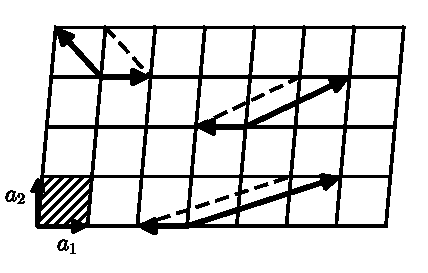
\includegraphics[width=6.5cm]{fig1-1.pdf}\\{\small 图 1.1\quad 二维点阵的元胞和基矢}
\end{minipage}
\end{center}

在三维情况下，元胞的体积为
\begin{equation}
  \Omega=\boldsymbol{a}_1\cdot(\boldsymbol{a}_2\times\boldsymbol{a}_3)
\end{equation}
应当指出，在固体物理学中还采用另一种外形较复杂的元胞.它是由一个格点与最近邻格点（有时也包括次近邻）的连线中垂面所围成的多面体，其中只包含一个结点，称为维格纳—赛茨元胞（简称W-S元胞），如图1.2所示.二维六角点阵的W-S元胞为正六边形，它比 $\boldsymbol{a}_1$、$\boldsymbol{a}_2$ 所组成的初基元胞更明显地反映出点阵的对称性.在三维情况下，简立方（sc）点阵的W-S元胞仍为立方体，体心立方（bcc）点阵的W-S元胞为截角八面体，面心立方点阵（fcc）则为菱十二面体，如图1.3所示.显然，W-S元胞是对称性元胞，它具有所属点阵点群的全部对称性.一切保持点阵不变的旋转、反射和反演操作都将同时保持W-S元胞不变，这为理论计算将带来方便.

\begin{center}
\begin{minipage}{5.5cm}
\centering
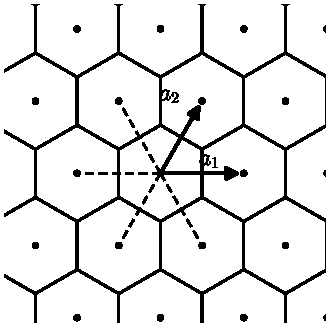
\includegraphics[width=5.5cm]{fig1-2.pdf}\\{\small 图 1.2\quad 二维六角点阵的W-S元胞}
\end{minipage}
\end{center}

由于晶体中的电子、声子、自旋波量子等元激发的状态都是用波矢量描述的，为便于讨论问题，又在波矢量空间人为地引入另一套点阵，称为倒点阵，它的长度量纲是坐标空间中长度量纲的倒数.倒点阵的基矢 $\boldsymbol{b}_i\,(i=1,2,3)$ 是由晶体点阵的基矢 $\boldsymbol{a}_i$ 按下列关系式定义的：
\begin{equation}
  \boldsymbol{a}_i\cdot\boldsymbol{b}_j=2\pi\delta_{ij}
  =\begin{cases}2\pi&(i=j)\\0&(i\neq j)\end{cases}
  \qquad(i,j=1,2,3)
\end{equation}

\begin{center}
\begin{minipage}{10.5cm}
\centering
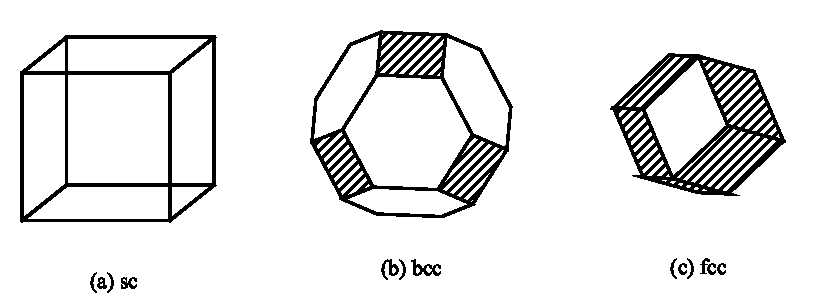
\includegraphics[width=10.5cm]{fig1-3.pdf}\\{\small 图 1.3\quad sc、bcc、fcc 点阵的W-S元胞}
\end{minipage}
\end{center}

容易求出 $\boldsymbol{b}_i$ 为
\begin{equation}
  \boldsymbol{b}_1=\frac{2\pi}{\Omega}(\boldsymbol{a}_2\times\boldsymbol{a}_3)\text{，}\quad
  \boldsymbol{b}_2=\frac{2\pi}{\Omega}(\boldsymbol{a}_3\times\boldsymbol{a}_1)\text{，}\quad
  \boldsymbol{b}_3=\frac{2\pi}{\Omega}(\boldsymbol{a}_1\times\boldsymbol{a}_2)
\end{equation}
在倒点阵中任一格点的位置矢
\begin{equation}
  \boldsymbol{K}_n=n_1\boldsymbol{b}_1+n_2\boldsymbol{b}_2+n_3\boldsymbol{b}_3
  =\sum_{i=1}^{3}n_i\boldsymbol{b}_i\qquad(n_i=\text{整数})
\end{equation}
称为倒格矢.与正点阵相似，倒点阵基矢 $\boldsymbol{b}_1$、$\boldsymbol{b}_2$、$\boldsymbol{b}_3$ 组成的平行六面体是倒点阵的元胞，它等于
\begin{equation}
  \Omega^{*}=\boldsymbol{b}_1\cdot(\boldsymbol{b}_2\times\boldsymbol{b}_3)
\end{equation}
为了便于讨论晶体对称性对电子、声子等能谱结构的影响，通常取倒点阵中相应的W-S元胞作为倒点阵的元胞.它是相对倒格点对称配置的多面体，在此多面体边界面上的任一点可由边界面上另一点加上一个倒格矢 $\boldsymbol{K}_n$ 的平移达到.当这个多面体的中心定为倒易空间的原点时，它所包含的区域称为第一布里渊区，用BZ表示，又称简约区.

倒点阵是根据正点阵作出的，它与正点阵有一一对应关系，其中正、倒点阵的元胞体积关系
\begin{equation}
  \Omega\Omega^{*}=(2\pi)^3
\end{equation}
和正、倒格矢之间的
\begin{equation}
  \boldsymbol{K}_n\cdot\boldsymbol{R}_l=2\pi\sum_{i=1}^{3}n_il_i=2\pi m
  \qquad(m=\text{整数})
\end{equation}
关系最为重要.

sc 正点阵的倒点阵仍为 sc，其 BZ 形状与图1.3(a)相同.fcc 正点阵的倒点阵为 bcc，其 BZ 形状如图1.3(b).bcc 正点阵的倒点阵为 fcc，其 BZ 形状与图1.3(c)同.

BZ是波矢量空间中的对称化元胞，它具有倒点阵点群的全部对称性，利用式(1.1.8)容易证明\footnote{其简单证明如下：设 $\alpha$ 为正点阵点群的对称操作，则 $\alpha\boldsymbol{R}_l$ 应为一个正格矢.由于群中有 $\alpha$ 必有逆操作 $\alpha^{-1}$，所以 $\alpha^{-1}\boldsymbol{R}_l$ 也应为一正格矢.根据式(1.1.8)应有
\begin{equation}
  \alpha^{-1}\boldsymbol{R}_l\cdot\boldsymbol{K}_n=2\pi m
\end{equation}
由于两矢量的点乘对于正交变换是不变的，上式可化为
\begin{equation}
  \boldsymbol{R}_l\cdot\alpha\boldsymbol{K}_n=2\pi m
\end{equation}
所以，对群中任意 $\alpha$ 而言，$\alpha\boldsymbol{K}_n$ 亦为一倒格矢，表明正、倒点阵具有相同点群对称性.}，同一晶体的正、倒点阵有相同的点群对称性，因此，可以简单地说，BZ具有晶体点阵点群的全部对称性.

\section{平移对称性}

点阵是格点在空间中的无限周期重复排列，点阵具有平移对称性，表现为将整体作任意正格矢的平移后，它将恢复原状；或者说，从空间任一点（并不一定是格点）出发，作任意正格矢的位移，必达到等效的点上.人们把晶体排列的周期性用抽象的几何点阵来表现，就是要赋予晶体平移不变的特征，使得含有大数粒子的完整晶体问题容易处理.平移对称性在固体物理学中占有十分重要的地位.

严格讲，只有无限理想晶体才具有平移对称性，实际晶体的尺寸都是有限的，边界面的存在必然会破坏平移对称性.但是，考虑到大块晶体的尺寸（如 $1\,\mathrm{cm}=10^{7}\,\mathrm{nm}$）总是比元胞的边长（$0.1\sim1\,\mathrm{nm}$）大 $10^{7}\sim10^{8}$ 量级，晶体体内的总粒子数也相应地比表面上粒子数大相同的量级；因此，当研究大块晶体特性时，表面效应并不重要，大块晶体的属性近似与边界条件的选择无关，于是可以设计一种特殊的边界条件，使有限晶体也具有平移不变性，这就是玻恩—卡门边界条件提出的背景.他们把3边长为 $N_1\boldsymbol{a}_1$、$N_2\boldsymbol{a}_2$、$N_3\boldsymbol{a}_3$ 的有限晶体设想为沿 $\boldsymbol{a}_1$、$\boldsymbol{a}_2$、$\boldsymbol{a}_3$ 3个方向上首尾相衔接的“环”，这样的配置规定了从晶体内的任一点平移 $N_1\boldsymbol{a}_1$、$N_2\boldsymbol{a}_2$、$N_3\boldsymbol{a}_3$ 必将再返回原处.这是一个循环条件，它相当于把无限多个晶体“复本”毫无缝隙地拼合在一起，组成一个无限晶体，图1.4是其一维示意图，这样做就保证了有限晶体也具有平移对称性.玻恩—卡门循环边界条件在数学上归结为 $N_i\boldsymbol{a}_i\,(i=1,2,3)$ 的平移操作是恒等操作，
\begin{equation}
  \{E|N_i\boldsymbol{a}_i\}=\{E|N_i\boldsymbol{a}_i\}^{-1}=\{E|0\}
\end{equation}

\begin{center}
\begin{minipage}{5cm}
\centering
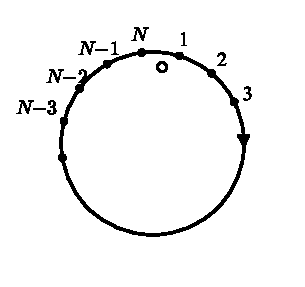
\includegraphics[width=5cm]{fig1-4.pdf}\\{\small 图 1.4\quad 波恩—卡门循环}
\end{minipage}
\end{center}

$\{E|\boldsymbol{R}_l\}$ 是平移算符，它对坐标的作用为
\begin{equation}
  \{E|\boldsymbol{R}_l\}\boldsymbol{r}=\boldsymbol{r}+\boldsymbol{R}_l\text{，}\quad
  \{E|\boldsymbol{R}_l\}^{-1}\boldsymbol{r}=\boldsymbol{r}-\boldsymbol{R}_l
\end{equation}
对函数的作用相应记为
\begin{equation}
\begin{aligned}
  \{E|\boldsymbol{R}_l\}f(\boldsymbol{r})
  &=f(\{E|\boldsymbol{R}_l\}^{-1}\boldsymbol{r})=f(\boldsymbol{r}-\boldsymbol{R}_l)\\
  \{E|\boldsymbol{R}_l\}^{-1}f(\boldsymbol{r})
  &=f(\{E|\boldsymbol{R}_l\}\boldsymbol{r})=f(\boldsymbol{r}+\boldsymbol{R}_l)
\end{aligned}
\end{equation}
对于元胞数为 $N=N_1N_2N_3$ 的晶体，共有 $N$ 个平移算符 $\{E|\boldsymbol{R}_l\}$，它们的集合满足群的组成条件：

(i) 任意两次相继的平移仍为一平移，即 $\{E|\boldsymbol{R}_1\}$ 乘 $\{E|\boldsymbol{R}_2\}$ 仍在 $\{E|\boldsymbol{R}_l\}$ 的集合之中.

(ii) 满足乘法的结合律.

(iii) 对每一个 $\{E|\boldsymbol{R}_l\}$，都存在 $\{E|\boldsymbol{R}_l\}^{-1}$，代表反方向的平移.$\{E|\boldsymbol{R}_l\}^{-1}$ 是 $\{E|\boldsymbol{R}_l\}$ 的逆元素.

(iv) 存在着恒等操作 $\{E|0\}$.

$\{E|\boldsymbol{R}_l\}$ 所组成的群叫平移群.平移群最重要的特征是相继两次平移的效果与它们作用的先后次序无关，即平移算符之间可对易，平移群是阿贝尔群.下面将讨论平移对称性对于晶体性能的影响.

\section{布洛赫定理}

当 $N\,(N=N_1N_2N_3)$ 个元胞的晶体满足玻恩—卡门条件时，具有平移对称性，其中正格矢 $\boldsymbol{R}_l=\sum_{i=1}^{3}l_i\boldsymbol{a}_i$ 可取 $N$ 个不同值，相应的有 $N$ 个平移算符 $\{E|\boldsymbol{R}_l\}$ 组成 $N$ 阶平移群.由于对所有的群元下列等式都成立，即
\begin{equation}
  \{E|\boldsymbol{R}_l\}^{-1}\{E|\boldsymbol{R}_m\}\{E|\boldsymbol{R}_l\}
  =\{E|\boldsymbol{R}_m\}
\end{equation}
故此 $N$ 阶群的每个元素本身自成一个共轭类.根据群论，群中共轭类数与不可约表示数相同.因此平移群有 $N$ 个不可约表示，不可约表示的维数 $n_\alpha$ 可由方程
\begin{equation}
  \sum_{\alpha=1}^{N}n_\alpha^2=N
\end{equation}
定出为 $n_\alpha\,(\alpha=1,2,\cdots,N)$，说明平移群的 $N$ 个不可约表示都是一维的.设 $\psi(\boldsymbol{r})$ 是此一维表示的基函数，则应有
\begin{equation}
\begin{aligned}
  &\{E|\boldsymbol{a}_j\}^{-1}\psi(\boldsymbol{r})
  =\psi(\{E|\boldsymbol{a}_j\}\boldsymbol{r})
  =\psi(\boldsymbol{r}+\boldsymbol{a}_j)
  =D(\{E|\boldsymbol{a}_j\})\psi(\boldsymbol{r})\\
  &\{E|\boldsymbol{a}_j\}^{-1}\{E|\boldsymbol{a}_j\}^{-1}\psi(\boldsymbol{r})
  =\{E|2\boldsymbol{a}_j\}^{-1}\psi(\boldsymbol{r})=D^2\psi(\boldsymbol{r})\\
  &\{E|N_j\boldsymbol{a}_j\}^{-1}\psi(\boldsymbol{r})
  =D^{N_j}\psi(\boldsymbol{r})\qquad(j=1,2,3)
\end{aligned}
\end{equation}
这里 $D$ 是表示的一维矩阵，实际上是一个数，利用循环边界条件式(1.2.1)得到
\begin{equation}
  D^{N_j}\psi(\boldsymbol{r})=\{E|N_j\boldsymbol{a}_j\}^{-1}\psi(\boldsymbol{r})
  =\{E|0\}\psi(\boldsymbol{r})=\psi(\boldsymbol{r})
\end{equation}
可求出
\begin{equation}
  D^{N_j}=1\text{，}\quad D=\exp\left(2\pi\mathrm{i}\frac{n_j}{N_j}\right)
\end{equation}
其中 $n_j=0,\pm1,\pm2,\cdots$.由此可知
\begin{equation}
\begin{aligned}
  \{E|\boldsymbol{R}_l\}^{-1}\psi(\boldsymbol{r})
  &=\psi(\boldsymbol{r}+\boldsymbol{R}_l)
  =\psi(\boldsymbol{r}+l_1\boldsymbol{a}_1+l_2\boldsymbol{a}_2+l_3\boldsymbol{a}_3)\\
  &=\exp\Bigl[2\pi\mathrm{i}\sum_{j=1}^{3}\left(l_jn_j/N_j\right)\Bigr]\psi(\boldsymbol{r})
\end{aligned}
\end{equation}
式(1.3.6)在倒易空间中定义一个波矢量
\begin{equation}
  \boldsymbol{k}\equiv\sum_{j=1}^{3}\frac{n_j}{N_j}\boldsymbol{b}_j
\end{equation}
对于任意正格矢的平移 $\boldsymbol{R}_l$，有
\begin{equation}
  \{E|\boldsymbol{R}_l\}^{-1}\psi(\boldsymbol{r})
  =\psi(\boldsymbol{r}+\boldsymbol{R}_l)
  =\mathrm{e}^{\mathrm{i}\boldsymbol{k}\cdot\boldsymbol{R}_l}\psi(\boldsymbol{r})
\end{equation}
由 $D$ 定义的波矢 $\boldsymbol{k}$ 可作为平移群不可约表示的标记，这里第 $\boldsymbol{k}$ 个不可约表示的一维矩阵是 $\exp(\mathrm{i}\boldsymbol{k}\cdot\boldsymbol{R}_l)$，式(1.3.8)也可以理解为平移算符的本征方程，$\exp(\mathrm{i}\boldsymbol{k}\cdot\boldsymbol{R}_l)$ 是它的第 $\boldsymbol{k}$ 个本征值，其本征函数相应的记为 $\psi_{\boldsymbol{k}}(\boldsymbol{r})$.因此，式(1.3.8)应当写为
\begin{equation}
  \{E|\boldsymbol{R}_l\}^{-1}\psi_{\boldsymbol{k}}(\boldsymbol{r})
  =\psi_{\boldsymbol{k}}(\boldsymbol{r}+\boldsymbol{R}_l)
  =\mathrm{e}^{\mathrm{i}\boldsymbol{k}\cdot\boldsymbol{R}_l}\psi_{\boldsymbol{k}}(\boldsymbol{r})
\end{equation}
此即布洛赫定理.布洛赫定理要求本征函数 $\psi_{\boldsymbol{k}}(\boldsymbol{r})$ 有特殊形式，因为式(1.3.9)可改写成下列对称形式：
\begin{equation*}
  \bigl[\mathrm{e}^{-\mathrm{i}\boldsymbol{k}\cdot(\boldsymbol{r}+\boldsymbol{R}_l)}
  \psi_{\boldsymbol{k}}(\boldsymbol{r}+\boldsymbol{R}_l)\bigr]
  =\bigl[\mathrm{e}^{-\mathrm{i}\boldsymbol{k}\cdot\boldsymbol{r}}
  \psi_{\boldsymbol{k}}(\boldsymbol{r})\bigr]\tag{1.3.9a}
\end{equation*}
这时若令
\begin{equation*}
  u_{\boldsymbol{k}}(\boldsymbol{r})
  =\bigl[\mathrm{e}^{-\mathrm{i}\boldsymbol{k}\cdot\boldsymbol{r}}
  \psi_{\boldsymbol{k}}(\boldsymbol{r})\bigr]
\end{equation*}
利用式(1.3.9a)可求出一个重要关系式
\begin{equation}
  u_{\boldsymbol{k}}(\boldsymbol{r}+\boldsymbol{R}_l)=u_{\boldsymbol{k}}(\boldsymbol{r})
\end{equation}
它说明 $u_{\boldsymbol{k}}(\boldsymbol{r})$ 是正点阵的周期函数.以 $u_{\boldsymbol{k}}(\boldsymbol{r})$ 为振幅的函数
\begin{equation}
  \psi_{\boldsymbol{k}}(\boldsymbol{r})
  =u_{\boldsymbol{k}}(\boldsymbol{r})\exp(\mathrm{i}\boldsymbol{k}\cdot\boldsymbol{r})
\end{equation}
称为布洛赫函数，它具有调幅波的特性.晶体周期势场中的电子波函数、格波、自旋波等都具有布洛赫函数的形式.因为，布洛赫定理是由晶体的平移对称性导出的，是共性的结论，凡属周期性结构中的波都应具有布洛赫函数的形式.

利用波矢 $\boldsymbol{k}$ 标记平移群的不可约表示，还存在非唯一性问题.当两个波矢 $\boldsymbol{k}$ 与 $\boldsymbol{k}'$ 相差任意倒格矢 $\boldsymbol{K}_n$ 时，
\begin{equation}
  \boldsymbol{k}'-\boldsymbol{k}=\boldsymbol{K}_n
\end{equation}
若将相应的布洛赫函数 $\psi_{\boldsymbol{k}}$ 与 $\psi_{\boldsymbol{k}'}$ 代入平移算符的本征方程式(1.3.9)，会得到相同的本征值
\begin{equation}
  \exp(\mathrm{i}\boldsymbol{k}'\cdot\boldsymbol{R}_l)
  =\exp(\mathrm{i}\boldsymbol{k}\cdot\boldsymbol{R}_l)
  \exp(\mathrm{i}\boldsymbol{K}_n\cdot\boldsymbol{R}_l)
  =\exp(\mathrm{i}\boldsymbol{k}\cdot\boldsymbol{R}_l)
\end{equation}
其中利用了 $\exp(\mathrm{i}\boldsymbol{K}_n\cdot\boldsymbol{R}_l)=1$，它来自关系式(1.1.8).因此，除 $\boldsymbol{k}$ 以外，还同时有一组与 $\boldsymbol{k}$ 等效的波矢 $\boldsymbol{k}+\boldsymbol{K}_n$ 对应于同一个不可约表示 $\exp(\mathrm{i}\boldsymbol{k}\cdot\boldsymbol{R}_l)$，即 $\exp(\mathrm{i}\boldsymbol{k}\cdot\boldsymbol{R}_l)$ 并不唯一地对应于 $\boldsymbol{k}$.为了消除 $\boldsymbol{k}$ 的非唯一性，应当限制 $\boldsymbol{k}$ 的取值范围以保证在此区域内任意两个波矢之差均小于一个最短的倒格矢.这样的区域就是第一布里渊区（BZ）.限于 BZ 内的波矢叫简约波矢，简约区体积为 $\Omega^{*}$，其中共有 $N$ 个不同的波矢 $\boldsymbol{k}$，它们可以唯一地标记平移群的 $N$ 个不可约表示.因此，第 $\boldsymbol{k}$ 个不可约表示可记为 $D^{(\boldsymbol{k})}(\{E|\boldsymbol{R}_l\})$，相应的特征标为
\begin{equation}
\begin{aligned}
  \chi^{(\boldsymbol{k})}\bigl(\{E|\boldsymbol{R}_l\}\bigr)
  &=T_{\mathrm{r}}D^{(\boldsymbol{k})}\bigl(\{E|\boldsymbol{R}_l\}\bigr)
  =D^{(\boldsymbol{k})}\bigl(\{E|\boldsymbol{R}_l\}\bigr)\\
  &=\exp\bigl(\mathrm{i}\boldsymbol{k}\cdot\boldsymbol{R}_l\bigr)
\end{aligned}
\end{equation}
通常简约区是取相对于 $\boldsymbol{k}=0$ 的对称多面体（倒空间W-S）元胞，有时为了推导方便，也对 $\boldsymbol{k}$ 采用限制条件
\begin{equation}
  -\pi<\boldsymbol{k}\cdot\boldsymbol{a}_i\leqslant\pi\qquad(i=1,2,3)
\end{equation}
根据式(1.3.7)满足这一限制的波矢也只有 $N$ 个.

下面从平移对称角度，讨论固体物理学中几个常用关系式：

(i)
\begin{equation}
  \sum_{\boldsymbol{R}_l}\exp[-\mathrm{i}(\boldsymbol{k}-\boldsymbol{k}')
  \cdot\boldsymbol{R}_l]=N\delta_{kk'}
\end{equation}
就是平移群不可约表示的正交关系.群论中两个不等价的不可约表示 $i$ 与 $j$ 的矩阵元满足正交关系
\begin{equation*}
  \sum_RD^{(i)*}_{\alpha\gamma}(R)D^{(j)}_{\beta\delta}(R)
  =\delta_{ij}\delta_{\alpha\beta}\delta_{\gamma\delta}\,\frac{g}{n_i}
\end{equation*}
其中 $g$ 为群的阶数，$n_i$ 为第 $i$ 个不可约表示的维数，求和遍及所有群元 $R$.对于平移群 $g=N$，$n_i=1$，$i\to\boldsymbol{k}$，$j\to\boldsymbol{k}'$，表示矩阵都是一维的 $D^{(\boldsymbol{k})}(\{E|\boldsymbol{R}_l\})=\exp[\mathrm{i}\boldsymbol{k}\cdot\boldsymbol{R}_l]$，这里 $\boldsymbol{k}$ 限于BZ，于是平移群不可约表示的正交关系为
\begin{equation*}
\begin{aligned}
  \sum_{\boldsymbol{R}_l}D^{(\boldsymbol{k})*}\bigl(\{E|\boldsymbol{R}_l\}\bigr)
  D^{(\boldsymbol{k}')}\bigl(\{E|\boldsymbol{R}_l\}\bigr)
  &=\sum_{\boldsymbol{R}_l}\exp\bigl[-\mathrm{i}(\boldsymbol{k}-\boldsymbol{k}')
  \cdot\boldsymbol{R}_l\bigr]\\
  &=N\delta_{kk'}
\end{aligned}
\end{equation*}
式(1.3.16)得证.

(ii)
\begin{equation}
  \sum_{\boldsymbol{k}\in\mathrm{BZ}}\exp\bigl[-\mathrm{i}\boldsymbol{k}
  \cdot(\boldsymbol{R}_l-\boldsymbol{R}_s)\bigr]
  =N\delta_{\boldsymbol{R}_l\boldsymbol{R}_s}
\end{equation}
代表平移群特征标的正交关系，群的特征标第二正交定理为
\begin{equation*}
  \sum_i\chi^{(i)*}(R)\chi^{(i)}(S)=\delta_{RS}\,\frac{g}{h_R}
\end{equation*}
其中 $h_R$ 是 $R$ 共轭类中元素数目.对于平移群各群元自成一类，群元 $R$、$S$ 分别对应于 $\{E|\boldsymbol{R}_l\}$、$\{E|\boldsymbol{R}_s\}$，根据式(1.3.14)
\begin{equation*}
  \chi^{(\boldsymbol{k})}\bigl(\{E|\boldsymbol{R}_l\}\bigr)
  =\exp\bigl(\mathrm{i}\boldsymbol{k}\cdot\boldsymbol{R}_l\bigr)\text{，}\quad
  \chi^{(\boldsymbol{k})}\bigl(\{E|\boldsymbol{R}_s\}\bigr)
  =\exp\bigl(\mathrm{i}\boldsymbol{k}\cdot\boldsymbol{R}_s\bigr)
\end{equation*}
因此其正交关系为
\begin{equation*}
\begin{aligned}
  \sum_{\boldsymbol{k}\in\mathrm{BZ}}
  \chi^{(\boldsymbol{k})*}\bigl(\{E|\boldsymbol{R}_l\}\bigr)
  \chi^{(\boldsymbol{k})}\bigl(\{E|\boldsymbol{R}_s\}\bigr)
  &=\sum_{\boldsymbol{k}}\exp\bigl[-\mathrm{i}\boldsymbol{k}
  \cdot(\boldsymbol{R}_l-\boldsymbol{R}_s)\bigr]\\
  &=N\delta_{\boldsymbol{R}_l\boldsymbol{R}_s}
\end{aligned}
\end{equation*}
这就是式(1.3.17)的群论证明，$\boldsymbol{k}\in\mathrm{BZ}$ 代表取简约波矢.因此，两个正交关系均来源于平移对称性，普遍适用于周期结构中的电子、声子和自旋波等.

\subsection*{(iii) 求和与积分关系}

由于沿倒点阵基矢 $\boldsymbol{b}_i$ 方向相邻 $\boldsymbol{k}$ 值的间距按式(1.3.7)为
\begin{equation*}
  \Delta\boldsymbol{k}_i=\frac{\boldsymbol{b}_i}{N_i}\qquad(i=1,2,3)
\end{equation*}
每一许可 $\boldsymbol{k}$ 值所占据的体积为
\begin{equation*}
  \Delta\boldsymbol{k}_1\cdot(\Delta\boldsymbol{k}_2\times\Delta\boldsymbol{k}_3)
  =\frac{\Omega^{*}}{N_1N_2N_3}
  =\frac{(2\pi)^3}{N\Omega}
  =\frac{(2\pi)^3}{V}
\end{equation*}
$V$ 为晶体体积.因此 $\boldsymbol{k}$ 空间单位体积内有 $\frac{V}{(2\pi)^3}$ 个不同波矢.由于 $N$ 很大，对 BZ 中许可波矢 $\boldsymbol{k}$ 的求和可按照下面的公式变换为对 $\boldsymbol{k}$ 的连续积分，即
\begin{equation}
  \sum_{\boldsymbol{k}}\left(\cdots\right)
  =\frac{V}{(2\pi)^3}\int\mathrm{d}^3k\left(\cdots\right)
\end{equation}
平移不变性对于晶体的能谱结构有重要影响.由于晶体结构的周期性，其哈密顿量 $H$ 与平移算符可对易，二者应有共同的本征函数.已经证明，平移算符的本征函数是布洛赫函数 $\psi_{\boldsymbol{k}}(\boldsymbol{r})$，它也应当是 $H$ 算符的本征函数.换句话说，$H$ 算符的本征函数和本征值均与简约波矢 $\boldsymbol{k}$ 有关，这就是群论中讲的按平移群的不可约表示对 $H$ 的本征函数分类.例如，在单电子问题中，平移对称性告诉我们，晶体中一个电子的运动状态由 $\psi_{\boldsymbol{k}}(\boldsymbol{r})=u_{\boldsymbol{k}}(\boldsymbol{r})\exp(\mathrm{i}\boldsymbol{k}\cdot\boldsymbol{r})$ 描述，求其相应的能量本征值则应求解定态薛定谔方程
\begin{equation}
  H\psi_{\boldsymbol{k}}(\boldsymbol{r})=E(\boldsymbol{k})\psi_{\boldsymbol{k}}(\boldsymbol{r})
\end{equation}
等式两边乘 $\exp(-\mathrm{i}\boldsymbol{k}\cdot\boldsymbol{r})$ 得
\begin{equation}
  H_{\boldsymbol{k}}u_{\boldsymbol{k}}(\boldsymbol{r})
  =E(\boldsymbol{k})u_{\boldsymbol{k}}(\boldsymbol{r})
\end{equation}
这里
\begin{equation}
\begin{aligned}
  H_{\boldsymbol{k}}
  &=\exp(-\mathrm{i}\boldsymbol{k}\cdot\boldsymbol{r})H
  \exp(\mathrm{i}\boldsymbol{k}\cdot\boldsymbol{r})\\
  &=H+\frac{\hbar^2k^2}{2m}-\frac{\mathrm{i}\hbar^2}{m}\boldsymbol{k}\cdot\nabla
\end{aligned}
\end{equation}
相当于对 $H$ 作一个规范变换.方程(1.3.20)在波矢 $\boldsymbol{k}$ 固定时由于满足条件 $u_{\boldsymbol{k}}(\boldsymbol{r})=u_{\boldsymbol{k}}(\boldsymbol{r}+\boldsymbol{R}_l)$，可简化为在正点阵的一个元胞中求解.这和鼓膜振动、势阱中粒子运动等问题相似，属于在有限区域内的厄米本征值问题，应有无穷个分立的本征值 $E_1(\boldsymbol{k})$，$E_2(\boldsymbol{k})$，$\cdots$，$E_n(\boldsymbol{k})$，$\cdots$.因此，晶体中单电子能量是 $\boldsymbol{k}$ 的多值函数.每一个确定的 $\boldsymbol{k}$ 描述一套能级 $\{E_n(\boldsymbol{k})\}$ 和状态 $\{\psi_{n\boldsymbol{k}}(\boldsymbol{r})\}$.这里 $\boldsymbol{k}$ 限于BZ，是取以 $\boldsymbol{k}=0$ 为中心的“W-S”元胞.必须注意，用 $\boldsymbol{k}$ 或 $\boldsymbol{k}+\boldsymbol{K}_n$ 作为平移群不可约表示的标记是等效的.我们也可以取倒格点 $\boldsymbol{K}_n$ 附近的W-S元胞作为波矢的限制区域，得出由 $\boldsymbol{k}+\boldsymbol{K}_n$ 描述的一套能级和波函数.这两套就全体而言应当相同，只要注意指标 $n$ 的编排总可以使得 $\boldsymbol{k}$ 点与 $\boldsymbol{k}+\boldsymbol{K}_n$ 点所标记的状态和能级一一对应，做到对于同一指标 $n$ 有
\begin{equation}
  \psi_{n,\boldsymbol{k}+\boldsymbol{K}_n}=\psi_{n,\boldsymbol{k}}
\end{equation}
\begin{equation}
  E_n(\boldsymbol{k}+\boldsymbol{K}_n)=E_n(\boldsymbol{k})
\end{equation}
这里明确规定了在倒易空间中 $\boldsymbol{k}$ 与 $\boldsymbol{k}+\boldsymbol{K}_n$ 代表同一个状态，对应相同的能量，可理解为同一点.由于在BZ外布洛赫函数本无新状态，因此式(1.3.23)相当于将 $E_n(\boldsymbol{k})$ 延拓到全 $\boldsymbol{k}$ 空间的一个约定条件，而允许 $\boldsymbol{k}$ 的取值遍及全 $\boldsymbol{k}$ 空间往往给处理问题带来方便.式(1.3.22)和式(1.3.23)告诉我们，当 $n$ 一定时的布洛赫函数及能量本征值是倒点阵的周期函数，这就是固体物理学中所说的周期能区图式.

既然确定 $n$ 值的 $E_n(\boldsymbol{k})$ 是倒点阵的周期函数，则必有能量的上、下界，使同一 $n$ 而不同 $\boldsymbol{k}$ 的所有能级包括在界内，从而组成一个能带.不同的 $n$ 代表不同的能带，它们的总体称为晶体的带结构.以上讨论说明，能带存在的结论是来自布洛赫波函数的振幅是正点阵的周期函数这一普遍性特征，因此，周期结构中一切波的能（频）谱都应成带.

\section{布里渊区和晶体对称性}

在本节中将讨论布里渊区中 $E_n(\boldsymbol{k})$ 的对称特性和简并度，这些问题涉及晶体的空间群\textsuperscript{[1,2]}.

空间群包含平移、旋转（正常及异常）、反射、滑移反映（位移＋反射）以及螺旋轴（位移＋旋转）等对称操作，由空间群算符 $\{\alpha|\boldsymbol{t}\}$ 表示，
\begin{equation}
  \{\alpha|\boldsymbol{t}\}\equiv\alpha\boldsymbol{r}+\boldsymbol{t}
\end{equation}
其中 $\alpha$ 代表旋转、反映等点群对称操作，$\boldsymbol{t}$ 代表平移.当 $\alpha$ 取单位元素 $E$ 及 $\boldsymbol{t}=\boldsymbol{R}_l$ 时，就是平移群 $\{E|\boldsymbol{R}_l\}$.无平移时，为 $\{\alpha|0\}$，代表点群.当 $\boldsymbol{t}\neq\boldsymbol{R}_l$ 时对应于螺旋轴或滑移反映面，是 $\alpha$ 操作与正格矢的分数平移 $\boldsymbol{\tau}$ 的组合 $\{\alpha|\boldsymbol{\tau}\}$.

由式(1.4.1)可证明空间群的两个算符的乘积为
\begin{equation}
  \{\alpha|\boldsymbol{t}\}\{\beta|\boldsymbol{s}\}
  =\{\alpha\beta|\alpha\boldsymbol{s}+\boldsymbol{t}\}
\end{equation}
$\{\alpha|\boldsymbol{t}\}$ 之逆为
\begin{equation}
  \{\alpha|\boldsymbol{t}\}^{-1}
  =\{\alpha^{-1}|-\alpha^{-1}\boldsymbol{t}\}
\end{equation}
晶体的空间群定义为：包括平移群作为不变子群的 $\{\alpha|\boldsymbol{t}\}$ 元素集合.取空间群的任意元素对平移群元素作下列乘积后得
\begin{equation}
  \{\alpha|\boldsymbol{t}\}\{E|\boldsymbol{R}_l\}\{\alpha|\boldsymbol{t}\}^{-1}
  =\{E|\alpha\boldsymbol{R}_l\}
\end{equation}
不变子群条件要求 $\alpha\boldsymbol{R}_l$ 仍为正格矢，换句话说点阵经旋转等点群操作后应与自身重合，这就限制了晶体中只可能出现2、3、4、6次旋转轴，使晶体空间群成为有限群.

\subsection*{1. BZ 中 $\boldsymbol{E}_n(\boldsymbol{k})$ 的对称性}

设晶体属于空间群 $\{\alpha|\boldsymbol{t}\}$，则晶体的哈密顿量 $H$ 应与 $\{\alpha|\boldsymbol{t}\}$ 对易，即 $H$ 对于空间群 $\{\alpha|\boldsymbol{t}\}$ 的一切操作是不变的，有对称性
\begin{equation}
  \{\alpha|\boldsymbol{t}\}^{-1}H\{\alpha|\boldsymbol{t}\}=H
\end{equation}
由式(1.4.4)可知
\begin{equation}
  \{E|\boldsymbol{R}_l\}\{\alpha|\boldsymbol{t}\}
  =\{\alpha|\boldsymbol{t}\}\{E|\alpha^{-1}\boldsymbol{R}_l\}
\end{equation}
这里还利用了式(1.4.2)和(1.4.3)，
\begin{equation}
\begin{aligned}
  \{E|\boldsymbol{R}_l\}\{\alpha|\boldsymbol{t}\}\psi_{n\boldsymbol{k}}(\boldsymbol{r})
  &=\{\alpha|\boldsymbol{t}\}\{E|\alpha^{-1}\boldsymbol{R}_l\}\psi_{n\boldsymbol{k}}(\boldsymbol{r})\\
  &=\{\alpha|\boldsymbol{t}\}\mathrm{e}^{-\mathrm{i}\boldsymbol{k}\cdot\alpha^{-1}\boldsymbol{R}_l}\psi_{n\boldsymbol{k}}
\end{aligned}
\end{equation}
等式左边利用了布洛赫定理[式(1.3.9)].由于对两个矢量作同一正交变换，其标量积不变，故应有
\begin{equation}
  \boldsymbol{k}\cdot\alpha^{-1}\boldsymbol{R}_l
  =\alpha[\boldsymbol{k}]\cdot\alpha(\alpha^{-1}\boldsymbol{R}_l)
  =\alpha[\boldsymbol{k}]\cdot\boldsymbol{R}_l
\end{equation}
于是式(1.4.7)写为
\begin{equation}
  \{E|\boldsymbol{R}_l\}\bigl(\{\alpha|\boldsymbol{t}\}\psi_{n\boldsymbol{k}}(\boldsymbol{r})\bigr)
  =\mathrm{e}^{-\mathrm{i}\alpha[\boldsymbol{k}]\cdot\boldsymbol{R}_l}
  \bigl(\{\alpha|\boldsymbol{t}\}\psi_{n\boldsymbol{k}}(\boldsymbol{r})\bigr)
\end{equation}
另一方面考虑BZ中波矢 $\boldsymbol{k}$ 经 $\alpha$ 操作后变为 $\alpha[\boldsymbol{k}]$，对应的布洛赫函数为 $\psi_{n,\alpha[\boldsymbol{k}]}(\boldsymbol{r})$，由于 $\alpha[\boldsymbol{k}]$ 仍在此BZ中，平移算符的本征方程应为
\begin{equation}
  \{E|\boldsymbol{R}_l\}\psi_{n,\alpha[\boldsymbol{k}]}(\boldsymbol{r})
  =\mathrm{e}^{-\mathrm{i}\alpha[\boldsymbol{k}]\cdot\boldsymbol{R}_l}
  \psi_{n,\alpha[\boldsymbol{k}]}(\boldsymbol{r})
\end{equation}
比较式(1.4.9)和(1.4.10)可知，函数 $\psi_{n,\alpha[\boldsymbol{k}]}(\boldsymbol{r})$ 与 $\{\alpha|\boldsymbol{t}\}\psi_{n,\boldsymbol{k}}(\boldsymbol{r})$ 具有相同的平移算符本征值 $\exp(-\mathrm{i}\alpha[\boldsymbol{k}]\cdot\boldsymbol{R}_l)$.由于平移群的不可约表示是一维的，这两个函数最多只差一个相位因子，应有关系式
\begin{equation}
  \psi_{n,\alpha[\boldsymbol{k}]}(\boldsymbol{r})
  =\lambda\{\alpha|\boldsymbol{t}\}\psi_{n,\boldsymbol{k}}(\boldsymbol{r})
  \qquad(|\lambda|^2=1)
\end{equation}
可求出 $\psi_{n,\alpha[\boldsymbol{k}]}(\boldsymbol{r})$ 的能量本征值
\begin{equation}
\begin{aligned}
  E_n(\alpha\boldsymbol{k})
  &=\int\psi^{*}_{n,\alpha[\boldsymbol{k}]}(\boldsymbol{r})
  H\psi_{n,\alpha[\boldsymbol{k}]}(\boldsymbol{r})\,\mathrm{d}^3\boldsymbol{r}\\
  &=\int\psi^{*}_{n,\boldsymbol{k}}(\boldsymbol{r})
  \{\alpha|\boldsymbol{t}\}^{-1}H\{\alpha|\boldsymbol{t}\}
  \psi_{n,\boldsymbol{k}}(\boldsymbol{r})\,\mathrm{d}^3\boldsymbol{r}\\
  &=\int\psi^{*}_{n,\boldsymbol{k}}(\boldsymbol{r})
  H\psi_{n,\boldsymbol{k}}(\boldsymbol{r})\,\mathrm{d}^3\boldsymbol{r}
  =E_n(\boldsymbol{k})
\end{aligned}
\end{equation}
注意，其中利用了经过晶体空间群操作后 $H$ 的不变性[式(1.4.5)]和空间群的幺正表式.

结论 $E_n(\alpha\boldsymbol{k})=E_n(\boldsymbol{k})$ 中，$\alpha$ 只是属于该晶体空间群（但未必就是点阵）的点群操作.因为，点阵只能有正格矢 $\boldsymbol{R}_l$ 的平移不变性，其所属空间群是 $\{\alpha|\boldsymbol{R}_l\}$.若取平移 $\boldsymbol{R}_l=0$（单位元素），可得 $\{\alpha|0\}$，它包括了点阵的全部点群操作，并构成简单空间群 $\{\alpha|\boldsymbol{R}_l\}$ 的子群.但是 $\{\alpha|0\}$ 并不一定是空间群 $\{\alpha|\boldsymbol{t}\}$ 的子群.当晶体具有螺旋轴或滑移反映面等组合操作时，$\alpha$ 的某些操作 $\beta$ 将与非整数的基矢平移 $\boldsymbol{\tau}_\beta$ 组合成群元 $\{\beta|\boldsymbol{\tau}_\beta\}$，这时 $\{\beta|0\}$ 将不是晶体的点群对称操作.因此，晶体的点群对称性也就低于 $\{\alpha|0\}$，即低于点阵的对称性.只有在简单空间群中，晶体和点阵才有相同的点群对称性.这时式(1.4.12)可以理解为：在每一能带中如果把能量 $E_n(\boldsymbol{k})$ 看作布里渊区中“位置”的函数（倒空间“位置”由 $\boldsymbol{k}$ 描述），它便具有点阵点群 $\{\alpha|0\}$ 的全部对称性，此即简单空间群中 $E_n(\boldsymbol{k})$ 的对称性.

由于点阵的全部点群对称性必然表现在由此点阵所定义的BZ的外形对称性中（详见§1），因此也可以说 BZ 具有 $\{\alpha|0\}$ 点群的全部对称性.所以，对于不存在组合操作的简单晶体或简单空间群，$E_n(\alpha\boldsymbol{k})=E_n(\boldsymbol{k})$ 就直接反映了布里渊区的对称性.

\begin{center}
\begin{minipage}{5.5cm}
\centering
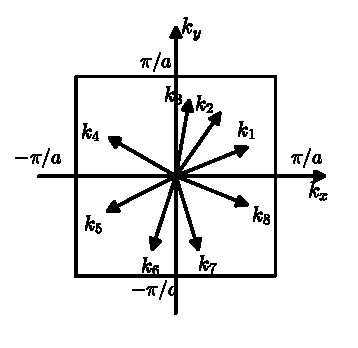
\includegraphics[width=5.5cm]{fig1-5.pdf}\\{\small 图 1.5}
\end{minipage}
\end{center}

例如二维正方点阵.BZ为正方形如图1.5，保持BZ不变的点群操作共有8个，它们是 $E$、$C_4$、$C_4^2$、$C_4^3$、$m_x$、$m_y$、$m_d$、$m_d'$，其中 $E$ 为恒等操作，$C_4$ 为垂直于纸面的4次轴，$m_x$、$m_y$ 分别为垂直于 $k_x$、$k_y$ 的对称面，$m_d$、$m_d'$ 是通过正方形两对角线的对称面.这8个元素组成的点群用 4mm 标记.

对于 BZ 中矢量 $\boldsymbol{k}_1$ 施以上述点群操作后，它将变到 $\boldsymbol{k}_1$、$\boldsymbol{k}_2$、$\cdots$、$\boldsymbol{k}_8$ 等8个点上去，这8个点在同一能带中有相同的能量
\begin{equation*}
  E_n(\boldsymbol{k}_1)=E_n(\boldsymbol{k}_2)=\cdots=E_n(\boldsymbol{k}_8)
\end{equation*}

\subsection*{2. $\boldsymbol{E}_n(\boldsymbol{k})$ 的简并度}

方程式(1.3.20)的本征值 $E_n(\boldsymbol{k})\,(n=1,2,3\cdots)$ 中可能有简并能级存在，设在 $\boldsymbol{k}$ 点第 $n$ 个能量本征值的简并度为 $d_n$，则应有 $d_n$ 个布洛赫函数 $\psi_{n,\boldsymbol{k},j}(\boldsymbol{r})\,(j=1,2,\cdots,d_n)$ 对应于同一个能量 $E_n(\boldsymbol{k})$.这种情况往往发生在BZ中某些高对称性的点与线上，这时点群中的某些元素对 $\boldsymbol{k}$ 运算后保持 $\boldsymbol{k}$ 不变（或等于 $\boldsymbol{k}+\boldsymbol{K}_n$）.这些群元对布洛赫函数作用将产生具有不同对称性的一组函数，它们同属方程式(1.3.20)的解，并且具有相同的 $\boldsymbol{k}$ 与能量 $E_n(\boldsymbol{k})$，这就是 $\psi_{n,\boldsymbol{k},j}(\boldsymbol{r})$ 的来源.为了确定能带 $E_n(\boldsymbol{k})$ 的简并度 $d_n$，人们引进 $\boldsymbol{k}$ 波矢群.

简单地说，$\boldsymbol{k}$ 波矢群就是点群 $\{\alpha|0\}$ 中使 $\boldsymbol{k}$ 不变（或变到相差倒格矢的等效点上去）的那些对称操作元素的集合所构成的群.这些操作满足条件
\begin{equation}
  \alpha\boldsymbol{k}=\boldsymbol{k}+\boldsymbol{K}_n
\end{equation}
它们组成一个点群，是 $\{\alpha|0\}$ 的子群.波矢群不可约表示的维数给出正交基函数的个数.由于同一不可约表示中各基函数有相同能量，因此 $\boldsymbol{k}$ 波矢群不可约表示的维数就等于 $\boldsymbol{k}$ 点能级的简并度 $d_n$.下面仍以二维正方点阵为例，说明如何从波矢群确定能级简并度.

又如二维正方点阵的波矢群，其BZ为正方形，保持BZ不变的对称操作属于点群 4mm，有 $E$、$C_4$、$C_4^2$、$C_4^3$、$m_x$、$m_y$、$m_d$、$m_d'$ 等8个对称操作元素.在 BZ 中有 6 个高对称性的点和线，它们是：(1)$\Gamma$、M、X 分别代表位于 BZ 中心（$\boldsymbol{k}=0$）、顶角及边界面中心的点；(2)$\Delta$、$\Sigma$、Z 分别代表位于线 $\Gamma$X、$\Gamma$M、XM 上任一点（但不包括 $\Gamma$、M、X），这6个点和线已标明于图1.6中.现在分别讨论各点的 $\boldsymbol{k}$ 波矢群及其不可约表示的维数：

\begin{center}
\begin{minipage}{5.5cm}
\centering
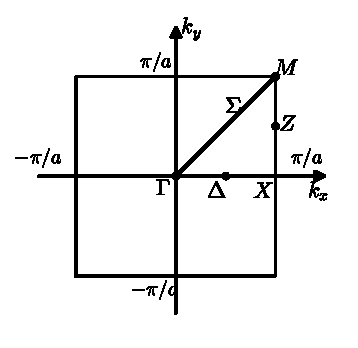
\includegraphics[width=5.5cm]{fig1-6.pdf}\\{\small 图 1.6\quad BZ 中高对称性的点与线}
\end{minipage}
\end{center}

\subsection*{(i) $\Gamma$ 点（$\boldsymbol{k}=0$）}

4mm 的 8 个对称操作均保持 $\boldsymbol{k}=0$ 不变，$\boldsymbol{k}=0$ 波矢群即点群 4mm，通常称为 $\Gamma$ 波矢群.这个群可分为5个共轭元素类，它们是：
\begin{equation*}
  E\text{、}\ C_4^2\text{、}\ C_4\text{、}C_4^3\text{、}\ m_x\text{、}m_y\text{、}\ m_d\text{、}m_d'
\end{equation*}
因此共有5个不同的不可约表示，这些表示的维数 $n_\alpha$ 应满足
\begin{equation*}
  \sum_{\alpha=1}^{5}n_\alpha^2=8
\end{equation*}
其解只可能是 $1^2+1^2+1^2+1^2+2^2=8$，说明在 $\Gamma$ 波矢群中有4个一维的和1个二维的不可约表示.因此在 $\Gamma$ 点 $E_n(0)$ 应有4种单重态和1种双重简并态.换句话说，在 $\Gamma$ 点可能有能带的二重简并发生.

\subsection*{(ii) M 点}

M 点波矢经 4mm 所有群元作用后仍在四顶角上（见图1.7），由于它们相差为倒格矢，满足条件(1.4.13)，因此 M 波矢群也是 4mm 点群，群阶 $g=8$.与 $\Gamma$ 波矢群相似，在 M 点也可能有双重简并能带出现.

\subsection*{(iii) X 点}

由于 X 点位于 $m_y$ 上，故 $m_y$ 操作不改变X，而 $m_x$ 和 $C_4^2$ 操作也只将 X 点变换到相差一倒格矢的对边中心（见图1.8）.按照式(1.4.13)，X波矢群应由 $E$、$m_x$、$m_y$、$C_4^2$ 等4个元素组成.这个群中各元素自成一个共轭类，因此有4个一维的不可约表示，说明在X点能带为非简并的.

\begin{center}
\begin{minipage}{4.5cm}
\centering
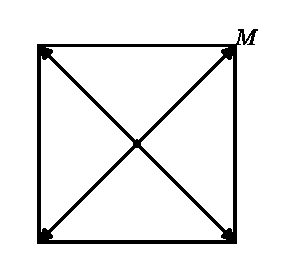
\includegraphics[width=4.5cm]{fig1-7.pdf}\\{\small 图 1.7}
\end{minipage}
\end{center}

\begin{center}
\begin{minipage}{4.5cm}
\centering
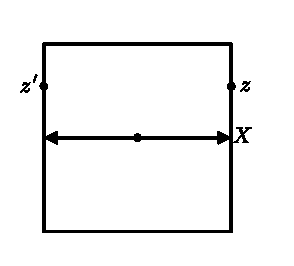
\includegraphics[width=4.5cm]{fig1-8.pdf}\\{\small 图 1.8}
\end{minipage}
\end{center}

\subsection*{(iv) $\Delta$、$\Sigma$、Z 点}

都只有两个元素组成波矢群，分别为 $\Delta$ 波矢群 $E$，$m_y$（$\Delta$ 位于 $m_y$ 上）；

$\Sigma$ 波矢群 $E$，$m_d$（$\Sigma$ 位于 $m_d$ 上）；

Z 波矢群 $E$，$m_x$[$m_x$ 操作将 $\boldsymbol{Z}\to\boldsymbol{Z}'$，两者差 $\frac{2\pi}{a}$，满足式(1.4.13)].

这些群中每个元素均自成一类，不可约表示都是一维的.在 $\Delta$、$\Sigma$、Z 上只有非简并的能带.

\subsection*{(v) BZ 中一般点 $\boldsymbol{k}_1$}

4mm 点群中除恒等元素 $E$ 外，其它7个操作将使 $\boldsymbol{k}_1$ 变为不同的波矢 $\boldsymbol{k}_2,\cdots,\boldsymbol{k}_8$（见图1.5）.波矢群只含单位元素 $E$，能带是非简并的.综上所述，在二维正方格子的布里渊区中，能带的简并只发生在BZ中心 $\Gamma$ 点与顶角M点上.

三维情况，当晶体空间群不包含滑移反映面及螺旋轴时，波矢群的分析可借助于32个点群的品格表，因为每波矢群属于32个点群之一，只需查出所对应点群品格表中恒等元素 $E$ 的特征标，即可得知波矢群不可约表示的维数，从而求得能带 $E_n(\boldsymbol{k})$ 的简并度.

到此为止，都认为对称关系
\begin{equation}
  E_n(\boldsymbol{k})=E_n(-\boldsymbol{k})
\end{equation}
是从空间反演对称性导出的.事实上，即使晶体不具空间反演对称（或换句话说，子群中不包含反演操作），例如在无对称中心的ZnS晶体中，其声子频率仍然满足式(1.4.14)，这是因为系统具有时间反演对称性.

\subsection*{3. 时间反演对称性}

时间反演是改变时间符号（$\boldsymbol{t}\to-\boldsymbol{t}$）的对称操作.由于无磁场时薛定谔方程对于时间反演操作具有不变性.因此，原来的状态和相应的时间反演态满足相同的方程，并具有同样的能量本征值.根据量子力学\textsuperscript{[3]}时间反演操作相当于：$\boldsymbol{r}\to\boldsymbol{r}$，$\boldsymbol{k}\to(-\boldsymbol{k})$ 和自旋反向 $\hat{\boldsymbol{s}}\to(-\hat{\boldsymbol{s}})$.对于晶体周期场中的单电子，当不计自旋影响时，能带用 $E_n(\boldsymbol{k})$ 表示.这样时间反演对称性即要求式(1.4.14)成立，而无需哈密顿量 $H(\boldsymbol{r})=H(-\boldsymbol{r})$——空间反演对称.将式(1.4.14)中 $E$ 换成 $\omega$，就表示声子频率的时间反演对称性.这是因为点阵力学建立在牛顿经典力学的基础上，经典力学的运动方程也具有时间反演不变性.

当考虑自旋对能谱影响时，布洛赫函数 $\psi_{n\uparrow}(\boldsymbol{k},\boldsymbol{r})$ 的时间反演态为 $\psi_{n\downarrow}(-\boldsymbol{k},\boldsymbol{r})$.量子力学已经证明，当不存在外磁场时，时间反演对称性要求上述两态满足同一个 $H$ 本征方程，并具有相同的能量本征值，这时式(1.4.14)应推广为
\begin{equation}
  E_{n\uparrow}(\boldsymbol{k})=E_{n\downarrow}(-\boldsymbol{k})
\end{equation}
这就是著名的克喇末（Kramers）定理.

值得注意的是，当晶体同时具有空间反演对称时，$E_{n\uparrow}(\boldsymbol{k})=E_{n\uparrow}(-\boldsymbol{k})$、$E_{n\downarrow}(\boldsymbol{k})=E_{n\downarrow}(-\boldsymbol{k})$ 与式(1.4.15)相结合得到
\begin{equation}
  E_{n\uparrow}(\boldsymbol{k})=E_{n\downarrow}(\boldsymbol{k})
\end{equation}
同一波矢 $\boldsymbol{k}$ 的两个不同自旋状态具有相同的能量，这一附加的两重自旋简并在固体理论中称为克喇末简并度.总之，时间反演对称性要求 $E_{n\uparrow}(\boldsymbol{k})=E_{n\downarrow}(-\boldsymbol{k})$，它是与系统的空间对称性无关的.

\section{点阵傅里叶级数}

在本节中，我们将介绍与周期性结构有关的基本数学公式，首先导出完整晶体中常用的傅里叶级数\textsuperscript{[4]}公式——点阵傅里叶级数.然后，介绍周期函数的格林定理\textsuperscript{[5]}.

\subsection*{1. 点阵傅里叶级数}

(i) 设函数 $f(\boldsymbol{r})$ 满足周期性边界条件
\begin{equation*}
  f(\boldsymbol{r})=f(\boldsymbol{r}+N_j\boldsymbol{a}_j)
\end{equation*}
其中 $\boldsymbol{a}_j\,(j=1,2,3)$ 代表正点阵基矢，$N_1N_2N_3=N$ 为元胞数，根据傅里叶展开的标准公式得到
\begin{equation}
  f(\boldsymbol{r})=(N\Omega)^{-\frac{1}{2}}\sum_{\boldsymbol{k}}f_{\boldsymbol{k}}
  \mathrm{e}^{\pm\mathrm{i}\boldsymbol{k}\cdot\boldsymbol{r}}
\end{equation}
\begin{equation}
  f_{\boldsymbol{k}}=(N\Omega)^{-\frac{1}{2}}\int_{N\Omega}\mathrm{d}\boldsymbol{r}\,
  f(\boldsymbol{r})\,\mathrm{e}^{\mp\mathrm{i}\boldsymbol{k}\cdot\boldsymbol{r}}
\end{equation}
推导式(1.5.2)时利用了关系式
\begin{equation}
  \int_{N\Omega}\mathrm{d}\boldsymbol{r}\,\mathrm{e}^{\pm\mathrm{i}\boldsymbol{k}\cdot\boldsymbol{r}}
  =(N\Omega)\,\delta_{\boldsymbol{k},0}
\end{equation}
其中 $\Omega$ 代表元胞体积，$\boldsymbol{k}$ 为满足周期性边界条件的波矢，式(1.5.1)中 $\sum_{\boldsymbol{k}}$ 是对所有的许可 $\boldsymbol{k}$ 值求和.

(ii) 设 $f(\boldsymbol{r})$ 是正点阵的周期函数
\begin{equation}
  f(\boldsymbol{r})=f(\boldsymbol{r}+\boldsymbol{l})
\end{equation}
则不难证明 $f(\boldsymbol{r})$ 可按倒格矢 $\boldsymbol{K}$ 展开为
\begin{equation}
  f(\boldsymbol{r})=\Omega^{-\frac{1}{2}}\sum_{\boldsymbol{K}}f_{\boldsymbol{K}}
  \mathrm{e}^{\pm\mathrm{i}\boldsymbol{K}\cdot\boldsymbol{r}}
\end{equation}
\begin{equation}
  f_{\boldsymbol{K}}=\Omega^{-\frac{1}{2}}\int_{\Omega}f(\boldsymbol{r})
  \mathrm{e}^{\mp\mathrm{i}\boldsymbol{K}\cdot\boldsymbol{r}}\,\mathrm{d}\boldsymbol{r}
\end{equation}
在证明上式时利用了正点阵周期函数 $f$ 的下列积分关系
\begin{equation}
\begin{aligned}
  I&=\int_{N\Omega}f(\boldsymbol{r})\mathrm{e}^{\pm\mathrm{i}\boldsymbol{k}\cdot\boldsymbol{r}}\,\mathrm{d}\boldsymbol{r}\\
  &=\sum_l\int_{\Omega}f(\boldsymbol{\rho})
  \mathrm{e}^{\pm\mathrm{i}\boldsymbol{k}\cdot(\boldsymbol{l}+\boldsymbol{\rho})}\,\mathrm{d}\boldsymbol{\rho}\\
  &=\Bigl[\sum_l\mathrm{e}^{\pm\mathrm{i}\boldsymbol{k}\cdot\boldsymbol{l}}\Bigr]
  \int_{\Omega}f(\boldsymbol{\rho})
  \mathrm{e}^{\pm\mathrm{i}\boldsymbol{k}\cdot\boldsymbol{\rho}}\,\mathrm{d}\boldsymbol{\rho}\\
  &=
  \begin{cases}
    N\displaystyle\int_{\Omega}f(\boldsymbol{\rho})
    \mathrm{e}^{\pm\mathrm{i}\boldsymbol{k}\cdot\boldsymbol{\rho}}\,\mathrm{d}\boldsymbol{\rho}
    &(\text{当 }\boldsymbol{k}=\boldsymbol{K}\text{ 倒格矢时})\\[1em]
    0&(\text{当 }\boldsymbol{k}\neq\boldsymbol{K}\text{ 时})
  \end{cases}
\end{aligned}
\end{equation}
因此，式(1.5.1)中傅里叶展开系数只取 $f_{\boldsymbol{K}}$，这就是式(1.5.5).

(iii) 当 $f$ 只在正格点 $\boldsymbol{l}$ 上定义时，式(1.5.1)直接简化为
\begin{equation}
  f(\boldsymbol{l})=(N\Omega)^{-\frac{1}{2}}\sum_{\boldsymbol{k}\in\mathrm{BZ}}f_{\boldsymbol{k}}
  \mathrm{e}^{\pm\mathrm{i}\boldsymbol{k}\cdot\boldsymbol{l}}
\end{equation}
式(1.5.8)用于晶格振动，推导时利用了 $\boldsymbol{K}\cdot\boldsymbol{l}=2\pi$（整数）.式(1.5.8)的逆傅里叶变换容易求出，将上式乘以 $N^{-\frac{1}{2}}\mathrm{e}^{\mp\mathrm{i}\boldsymbol{k}\cdot\boldsymbol{l}}$，再对 $\boldsymbol{l}$ 求和：
\begin{equation*}
\begin{aligned}
  &N^{-\frac{1}{2}}\sum_l f(\boldsymbol{l})\mathrm{e}^{\mp\mathrm{i}\boldsymbol{k}\cdot\boldsymbol{l}}\\
  &\quad=\Omega^{-\frac{1}{2}}\sum_{\boldsymbol{k}'\in\mathrm{BZ}}f_{\boldsymbol{k}'}
  \Bigl\{\frac{1}{N}\sum_l\mathrm{e}^{\pm\mathrm{i}(\boldsymbol{k}'-\boldsymbol{k})\cdot\boldsymbol{l}}\Bigr\}\\
  &\quad=\Omega^{-\frac{1}{2}}\sum_{\boldsymbol{k}'\in\mathrm{BZ}}f_{\boldsymbol{k}'}
  \delta_{\boldsymbol{k},\boldsymbol{k}'}=\Omega^{-\frac{1}{2}}f_{\boldsymbol{k}}
\end{aligned}
\end{equation*}
因此
\begin{equation}
  f_{\boldsymbol{k}}=\left(\frac{\Omega}{N}\right)^{\frac{1}{2}}\sum_l f(\boldsymbol{l})
  \mathrm{e}^{\mp\mathrm{i}\boldsymbol{k}\cdot\boldsymbol{l}}
\end{equation}
(iv) 当 $f$ 是 $\boldsymbol{k}$ 空间的函数，并满足
\begin{equation}
  f(\boldsymbol{k})=f(\boldsymbol{k}+\boldsymbol{K})
  \qquad(\boldsymbol{K}\ \text{是倒格矢})
\end{equation}
时，若令式(1.5.8)和(1.5.9)中
\begin{equation*}
  \Omega^{-\frac{1}{2}}f_{\boldsymbol{k}}\to f(\boldsymbol{k})
\end{equation*}
则得到关系式
\begin{equation}
  f(\boldsymbol{k})=N^{-\frac{1}{2}}\sum_l f(\boldsymbol{l})
  \mathrm{e}^{\mp\mathrm{i}\boldsymbol{k}\cdot\boldsymbol{l}}
\end{equation}
和
\begin{equation}
  f(\boldsymbol{l})=N^{-\frac{1}{2}}\sum_{\boldsymbol{k}\in\mathrm{BZ}}f(\boldsymbol{k})
  \mathrm{e}^{\pm\mathrm{i}\boldsymbol{k}\cdot\boldsymbol{l}}
\end{equation}
式(1.5.11)就倒点阵周期函数按正格矢 $\boldsymbol{l}$ 展开的点阵傅里叶级数，用于瓦尼尔（Wannier）函数.

\subsection*{2. 周期函数的格林定理}

设 $u(\boldsymbol{r})$ 与 $v(\boldsymbol{r})$ 均为正点阵的周期函数，则下列等式成立
\begin{equation}
  \int_{\Omega}\mathrm{d}\tau\,u\,\nabla v
  =-\int_{\Omega}\mathrm{d}\tau\,v\,\nabla u
\end{equation}
\begin{equation}
  \int_{\Omega}\mathrm{d}\tau\,u\nabla^2v
  =\int_{\Omega}\mathrm{d}\tau\,v\nabla^2u
\end{equation}
其中 $\Omega$ 为元胞体积，式(1.5.13)和(1.5.14)可称为周期函数的格林定理.

[证明]设 $f(\boldsymbol{r})$ 为任意函数，具有正点阵的周期性，它在元胞 $\Omega$ 内的积分
\begin{equation}
  I(\boldsymbol{r}')=\int_{\Omega}\mathrm{d}\tau\,f(\boldsymbol{r}+\boldsymbol{r}')
\end{equation}
应与 $\boldsymbol{r}'$ 无关，因此 $I(\boldsymbol{r}')$ 对 $\boldsymbol{r}'$ 的一、二阶导数必为零，于是有关系式
\begin{equation}
  \nabla'I(\boldsymbol{r}')
  =\int_{\Omega}\mathrm{d}\tau\,\nabla'f(\boldsymbol{r}+\boldsymbol{r}')
  =\int_{\Omega}\mathrm{d}\tau\,\nabla f(\boldsymbol{r}+\boldsymbol{r}')=0
\end{equation}
\begin{equation}
  \nabla'^2I(\boldsymbol{r}')
  =\int_{\Omega}\mathrm{d}\tau\,\nabla'^2f(\boldsymbol{r}+\boldsymbol{r}')
  =\int_{\Omega}\mathrm{d}\tau\,\nabla^2 f(\boldsymbol{r}+\boldsymbol{r}')=0
\end{equation}
再令 $\boldsymbol{r}'=0$，则求得周期函数 $f(\boldsymbol{r})$ 满足
\begin{equation}
  \int_{\Omega}\mathrm{d}\tau\,\nabla f(\boldsymbol{r})=0
\end{equation}
\begin{equation}
  \int_{\Omega}\mathrm{d}\tau\,\nabla^2 f(\boldsymbol{r})=0
\end{equation}
若假设
\begin{equation}
  f(\boldsymbol{r})=u(\boldsymbol{r})v(\boldsymbol{r})
\end{equation}
代入式(1.5.18)，即求得式(1.5.13)，代入式(1.5.19)有
\begin{equation}
  \int_{\Omega}\mathrm{d}\tau\bigl[u\nabla^2v+v\nabla^2u
  +2\nabla u\cdot\nabla v\bigr]=0
\end{equation}
再设 $v$ 与 $\nabla u$ 组成式(1.5.13)中两个周期函数，可得关系式
\begin{equation}
  2\int_{\Omega}\mathrm{d}\tau\,\nabla u\cdot\nabla v
  =-2\int_{\Omega}\mathrm{d}\tau\,u\,\nabla^2v
\end{equation}
将式(1.5.22)代入式(1.5.21)即证明了式(1.5.14).

周期函数的格林定理在能带理论中有重要应用.

\begin{canKao}
\begin{enumerate}[label={[\arabic*]}, leftmargin=2.2em, itemsep=0pt]
\item Morgan D J. Group Theory and Electron State in Perfect Crystals. In: Landsberg P T, ed. Solid State Theory. London: Wiley-Interscience, 1969
\item Callaway J. Quantum Theory of Solid State. New York: Academic Press, 1976. Chap 3
\item Merzbacher E. Quantum Mechanics (2nd ed). New York: John Wiley and Sons Inc, 1970. Chap 16
\item Landsberg P T. Solid State Theory. London: Wiley-Interscience, 1969. Chap 2
\item Aschroft N W, Mermin N D. Solid State Physics. New York: Holt, Rinehart and Winston, 1976
\end{enumerate}
\end{canKao}

% ============================================================
%  第二章 声子（§1–§10 + 章末参考文献）
%  底本：高等教育出版社《固体理论》（第二版）印刷页 18–61（PDF p038–p081）
%  OCR 输入：MinerU/full_merged.md 行 1142–3226
%  公式编号自检：§1 (2.1.1)–(2.1.27)；§2 (2.2.1)–(2.2.34)；
%    §3 (2.3.1)–(2.3.13)；§4 (2.4.1)–(2.4.24)；§5 (2.5.1)–(2.5.31)；
%    §6 (2.6.1)–(2.6.28)；§7 (2.7.1)–(2.7.17)；§8 (2.8.1)–(2.8.22)；
%    §9 (2.9.1)–(2.9.29)；§10 (2.10.1)–(2.10.34)。
%    共 259 个自动编号（OCR 有 258 个 tag：(2.2.25) 内容被 OCR 漏失，
%    按原书 p046 补排；(2.4.2) OCR tag 残缺为 {4.2}，原书 p052 有此式，
%    自动编号复原）。逐一对上，无跳号。
%  已修正的 OCR/原书错误：
%  1. 章首段"振动—晶格振动"按原书 p038 补全破折号为"振动——晶格振动"
%  2. (2.1.1) OCR 误作 X_l(t)=\dot R_l+u_l(t)，原书 p038 为 R_l（无点）
%  3. (2.1.3) 第二个求和下标 OCR 误作 l,β，原书为 l',β；(2.1.8) 同此（r→l'）
%  4. (2.1.10) OCR 漏下标：e^{ik·R}→e^{ik·R_l}
%  5. 行内"是沿 α(α=x,y,z) 方向的位移分量"OCR 乱码按原书 p038 复原
%  6. "由于式(2.1.6)并考虑到势能Φ为实函数……反演对称性后"OCR 串入
%     \barΦ/Φ 乱码，按原书 p040 复原
%  7. (2.1.20)–(2.1.24) 复式晶格诸式 OCR 乱码严重，按原书 p041 以
%     \binom{k}{s,s'} 记法复原；(2.1.26)/(2.1.27) 附近 M_s 错位同此
%  8. "构成3r维空间的本征矢量X_σ"OCR 漏 X_σ，按原书 p042 补
%  9. (2.2.3)/(2.2.4) 求和指标 n_l→R_l，首行指数 e^{-ik·R_l}→e^{-iαk·R_l}，
%     第二行 e^{-ik·e^{-1}R_l}→e^{-ik·α^{-1}R_l}（原书 p042）
% 10. "与传播方向方平行"原书 p046 排印衍一"方"字，删
% 11. "则本方征方程式(2.2.8)变为"原书 p043 排印错误，"本方征"→"本征"
% 12. (2.2.25) 原书为极化矢量式（p046），OCR 只剩编号，已按原书补排；
%     (2.2.24) 的频率两行原书共用一号，按原书排为一号
% 13. (2.2.22) OCR 拆成两个 $$ 块（ω₁² 行无号），原书共用 (2.2.22)，
%     按原书合并；(2.2.28)/(2.2.31)/(2.2.34) 同类处理
% 14. (2.2.29)/(2.2.30) OCR 矩阵/根式乱码，按原书 p048 复原
% 15. "例如二维正方晶格的 ω_σ(k) 和 e_{kσ} 的计算……计算准至第二近邻"
%     及"其中 f_l=f₁(l=1,2,3,4), f_l=f₂(l=5,6,7,8)"OCR 乱码按原书 p044 复原
% 16. "有两支频谱 ω_±²(k)，其中由于 ω₋(k=0)=0……而 ω₊ 则代表光频支格波"
%     OCR 丢 ω₋/ω₊ 下标，按原书 p049 复原
% 17. §3 脚注①（"也可以约定 e_{kσ}=−e_{−kσ}，则 Q*_{kσ}=−Q_{−kσ}，其结果
%     相同."）整段被 OCR 漏失，按原书 p049 页脚补录
% 18. (2.3.11) OCR 作 e_{kα}^α，原书 p051 为 e_{kσ}^{α*}；(2.3.13) 同此
% 19. (2.4.2) OCR tag 残缺为 {4.2}；且原书 p052 两处极化矢量漏印共轭星号
%     （无星号则中间步推不出 δ_σσ'），按物理补 e_{kσ}^{α*}
% 20. (2.4.11) OCR 作 \tilde{=}，原书 p053 为等号
% 21. (2.4.15) 之后 ε'_n=nℏω 一行 OCR 漏"(n=1,2,3,⋯)"，按原书 p054 补
% 22. §4 末段"和动量 ℏk 的玻色粒子"OCR 误作"动量kk"；"|{n_{kσ}}>"态
%     记号乱码按原书 p056 复原
% 23. §5 "引入一个在空间缓变的位移场"OCR 误作"引人"；"u 就是 l 元胞中
%     质心的位移"OCR 误作"μ 就是"；均按原书 p056 改
% 24. §5 "只可能有 ∇·u、∇u 及 ∇×u 三种一阶导数"OCR 乱码（∇μ、串入
%     u(r)），按原书 p057 复原；"把晶体当作弹性各向同性体"OCR 串入 φ(r)，删
% 25. (2.5.8) 第二行漏 Σ_{μ,ν}，按原书 p057 补
% 26. "当然，严格的作法应从 ℒ=𝒯−φ 的拉格朗日方程导出"OCR 乱码按原书 p058 复原
% 27. (2.5.24) 第二行 OCR 作 ρ(r)，原书 p059 为动量场 p(r)；"它等于 Q̇*_{kσ}"
%     及"约定关系式(2.3.3)和(2.3.4)保持不变"OCR 错位按原书复原
% 28. "再作变换，引入声子的产生及消灭算符"OCR 串入 \vec{p}，删（原书 p059）
% 29. §5 脚注①（体积相对变化 Δ=δV/V=∇·u 推导）被 OCR 误置于 §6 正文，
%     按原书 p060 页脚归位为脚注；OCR 之 δ̃V、∂u^s/∂x 等乱码同此复原
% 30. §6 "M_± 为正、负离子的质量"OCR 漏下标 ±；"电荷量相等、符号相反的
%     离子"OCR 串入 \barπ，均按原书 p060 复原
% 31. (2.6.4)–(2.6.8) 的下标"弹性/极化"OCR 乱码，按原书 p061 复原为
%     \text{弹性}/\text{极化}
% 32. "(如高、低频介电常数 ε_∞、ε_0 等)"OCR 乱码按原书 p062 复原；
%     (2.6.16) 末尾 OCR 多一逗号，删
% 33. §7 首段"光子波数 k=ω/c=ω_T/c"OCR 误作"k:ω/c=…"；ω_±(k) 的 ±
%     下标多处脱落（含 (2.7.6) 前后特征 (i)(ii)(iii) 段），按原书 p064–p066 复原
% 34. §7 特征段"对于大 k 值"OCR 误作"大 h 值"；"ω₋类光及 ω₊类声"按原书复原
% 35. 图 2.8/2.9/2.10 三图原书并排于 p066，图注照录；OCR 之一幅无注图按
%     原书归位（裁剪图 hash 重复不影响占位排版）
% 36. (2.8.8) 求导下标 OCR 作"\_"，按原书 p068 补 V
% 37. (2.8.13) 第二行积分上限 OCR 作 ∞，原书 p069 为 ω_M
% 38. §8–§9 \underline{ĝ}、δ̂、\widehat\otimes 等噪声统一为 g、δ
% 39. "算出的态密集为"原书 p074 排印错误，"态密集"→"态密度"
% 40. §10 "影响. 从一维原子链入手"OCR 逗号按原书 p075 改句号；
%     (2.10.6) 整式乱码按原书 p076 复原为 u_l=(1/√N)Σ_k ξ_k e^{-ikla}
% 41. (2.10.12) OCR 串入 \pounds_k，按原书 p077 改回 ξ_k
% 42. §10 "式(2.10.14)的解相对于 ω_k 都朝高频方向略有移动"OCR 漏下标 k，
%     按原书 p077 补；"分立能级——局域模"破折号按原书 p081 补全
% 43. 其余：全角句点"．"→"."；删除 OCR 间隔符"~"；\mathrm{d} 收紧；
%     \pmb→\boldsymbol；§4/§7/§8 标题字间空格收紧
%  遗留问题：图 2.1–2.13 均为占位图（fig2-N.pdf），宽度按原书目测配置；
%  图 2.11 四联小图的 (a)–(d) 子图注含于占位图，未另排
% ============================================================
\chapter{声子}

\section{晶格动力学}

本节用经典力学方法讨论完整晶体中原子（离子）绕平衡位置的振动——晶格振动.为简单起见，先讨论每个元胞中只含一个原子(离子)的简单晶格情况，然后推广到含多个原子的复式晶格情况.

设晶体的元胞数为$N$，原子质量为$M$.晶体中第$l$个元胞中原子的平衡位置由正格矢$\boldsymbol{R}_l$描述，$\boldsymbol{u}_l$则代表此原子的位移.因此，在$t$时刻$l$元胞中原子的瞬时位置为
\begin{equation}
  \boldsymbol{X}_l(t)=\boldsymbol{R}_l+\boldsymbol{u}_l(t)\,,\quad
  \boldsymbol{R}_l=\sum_{i=1}^{3}l_i\boldsymbol{a}_i
\end{equation}
晶格振动的总动能
\begin{equation}
  T=\frac{1}{2}\sum_{l,\alpha}M\dot{u}_l^{\alpha}\dot{u}_l^{\alpha}
  \qquad(\alpha=x,y,z)
\end{equation}
这里$u_l^{\alpha}$是沿$\alpha\,(\alpha=x,y,z)$方向的位移分量.由于晶体中原子(离子)的运动限于微振动，其总势能可按$u_l^{\alpha}$展开表示
\begin{equation}
  \Phi=\Phi_0+\sum_{l,\alpha}\Phi_{\alpha}(l)u_l^{\alpha}
  +\frac{1}{2}\sum_{l,\alpha}\sum_{l',\beta}\Phi_{\alpha\beta}(l,l')u_l^{\alpha}u_{l'}^{\beta}+\cdots
\end{equation}
这里$\Phi_0$为一常数，代表晶体中所有原子都处于平衡位置时的势能，它对于晶格振动不起作用，而
\begin{equation}
  \Phi_{\alpha}(l)=\left(\frac{\partial\Phi}{\partial u_l^{\alpha}}\right)_0=0
\end{equation}
是由于在平衡点晶体的势能极小，其中下标0代表平衡点，宗量内的符号$l$是正格矢$\boldsymbol{R}_l$的缩写.$\Phi_{\alpha\beta}(l,l')$为二次导数
\begin{equation}
  \Phi_{\alpha\beta}(l,l')=\left(\frac{\partial^2\Phi}
  {\partial u_l^{\alpha}\partial u_{l'}^{\beta}}\right)_0
  =\Phi_{\beta\alpha}(l',l)
\end{equation}
其中最后一个等式来源于二次导数的对称性.当采用周期性边界条件时，晶体具有平移不变性，$\Phi_{\alpha\beta}(l,l')$只是$(\boldsymbol{R}_l-\boldsymbol{R}_{l'})$的函数.计入平移对称性后，上式可写为
\begin{equation}
  \Phi_{\alpha\beta}(l,l')=\Phi_{\alpha\beta}(l-l')=\Phi_{\beta\alpha}(l'-l)
\end{equation}
$\Phi_{\alpha\beta}(l-l')$代表$l'$元胞中原子沿$\beta$方向位移单位距离时对$l$元胞中原子作用力沿$\alpha$方向的分量，称为力常数，并有下列重要关系：
\begin{equation}
  \sum_{l'}\Phi_{\alpha\beta}(l-l')=0
\end{equation}
因为当整体作刚性位移(即每个原子均作$u_l^{\alpha}=v_{\alpha}$的位移)时，晶格中任一原子受到其它原子作用力之总和为零，即
\begin{equation*}
\begin{aligned}
  F_{\alpha}(l)&=-\frac{\partial\Phi}{\partial u^{\alpha}}
  =-\sum_{l',\beta}\Phi_{\alpha\beta}(l-l')u_{l'}^{\beta}\\
  &=-\sum_{\beta}\Bigl\{\sum_{l'}\Phi_{\alpha\beta}(l-l')\Bigr\}v_{\beta}=0
\end{aligned}
\end{equation*}
由于刚性位移量$v_{\beta}$可取任意值，因此上式中$\{\cdots\}=0$，此即关系式(2.1.7).

在简谐近似下，略去$\Phi$按位移$u$展开的三次方项，定义$\Delta\Phi=\Phi-\Phi_0$，则系统的振动哈密顿量为
\begin{equation}
  H=T+\Delta\Phi=\frac{1}{2M}\sum_{l,\alpha}p_l^{\alpha}p_l^{\alpha}
  +\frac{1}{2}\sum_{l,\alpha}\sum_{l',\beta}\Phi_{\alpha\beta}(l-l')u_l^{\alpha}u_{l'}^{\beta}
\end{equation}
其中$p_l^{\alpha}=M\dot{u}_l^{\alpha}$是$u_l^{\alpha}$的共轭力学量.系统的运动方程由经典力学的正则方程$\dot{p}_l^{\alpha}=-(\partial H/\partial u_l^{\alpha})$导出
\begin{equation}
  M\ddot{u}_l^{\alpha}=-\sum_{l',\beta}\Phi_{\alpha\beta}(l-l')u_{l'}^{\beta}
\end{equation}
其中利用了对称关系式(2.1.6).式(2.1.9)是$3N$个自由度的线性耦合振动方程组.利用平移对称性可使求解大为简化.将布洛赫定理，式(1.3.9)，用于晶格振动$u_l^{\alpha}$，应有
\begin{equation}
  u_l^{\alpha}=\mathrm{e}^{\mathrm{i}\boldsymbol{k}\cdot\boldsymbol{R}_l}u_0^{\alpha}
\end{equation}
对于每一确定$\boldsymbol{k}$值，运动方程的解表现出下列特性：

(i)各元胞中原子振动的方向相同，振幅相等；

(ii)有特定的相位关系，按$\mathrm{e}^{\mathrm{i}\boldsymbol{k}\cdot\boldsymbol{R}_l}$变化.

因此，每一确定$\boldsymbol{k}$的解代表波长为$\frac{2\pi}{|\boldsymbol{k}|}$的集体振动，称为格波.对于每一个$\boldsymbol{k}$，可确定方程式(2.1.9)的一个特解
\begin{equation*}
  \mathrm{e}^{\mathrm{i}\boldsymbol{k}\cdot\boldsymbol{R}_l}U_{\boldsymbol{k}}^{\alpha}
\end{equation*}
这里，令$u_0^{\alpha}=U_{\boldsymbol{k}}^{\alpha}$对应于用波矢$\boldsymbol{k}$标记的特解，将它代入式(2.1.9)，可将$3N$自由度的耦合方程组简化为$N$个独立的3自由度耦合方程组，而每个波矢满足方程：
\begin{equation}
  \ddot{U}_{\boldsymbol{k}}^{\alpha}=-\sum_{\beta}D_{\alpha\beta}(\boldsymbol{k})U_{\boldsymbol{k}}^{\beta}
  \quad(\alpha,\beta=x,y,z)
\end{equation}
其中
\begin{equation}
  D_{\alpha\beta}(\boldsymbol{k})\equiv\frac{1}{M}\sum_{l}\Phi_{\alpha\beta}(\boldsymbol{l})
  \mathrm{e}^{-\mathrm{i}\boldsymbol{k}\cdot\boldsymbol{R}_l}
\end{equation}
组成$3\times3$矩阵，代表力常数$\Phi$的傅里叶变换称为动力矩阵.由于式(2.1.6)并考虑到势能$\Phi$为实函数，易知，对于简单晶格考虑反演对称性后，$D_{\alpha\beta}(\boldsymbol{k})$应为实的厄米矩阵，其对角化方程(又称动力矩阵的本征方程)为
\begin{equation}
  \sum_{\beta}D_{\alpha\beta}(\boldsymbol{k})e_{\boldsymbol{k}}^{\beta}
  =\omega^2e_{\boldsymbol{k}}^{\alpha}
\end{equation}
这里，当$\omega$理解为振动频率时，$\omega^2$取正实量，具体由久期方程决定
\begin{equation}
  \det\parallel D_{\alpha\beta}(\boldsymbol{k})-\omega^2\delta_{\alpha\beta}\parallel=0
\end{equation}
可求出3个本征值
\begin{equation}
  \omega=\omega_{\sigma}(\boldsymbol{k})\qquad(\sigma=1,2,3)
\end{equation}
以及相应的3个实本征向量$\boldsymbol{e}_{\boldsymbol{k}\sigma}$，它们是描述各元胞中原子振动方向的单位矢，并满足下列正交性和完备性条件：
\begin{equation}
  \boldsymbol{e}_{\boldsymbol{k}\sigma}\cdot\boldsymbol{e}_{\boldsymbol{k}\sigma'}=\delta_{\sigma\sigma'}
\end{equation}
\begin{equation}
  \sum_{\sigma}e_{\boldsymbol{k}\sigma}^{\alpha}e_{\boldsymbol{k}\sigma}^{\beta}=\delta_{\alpha\beta}
\end{equation}
显然，利用式(2.1.13)可将运动方程式(2.1.11)退耦，并求出$U_{\boldsymbol{k}}^{\alpha}$正比于$e_{\boldsymbol{k}}^{\alpha}\mathrm{e}^{-\mathrm{i}\omega t}$的解.代入式(2.1.10)，有形式为
\begin{equation*}
  u_l^{\alpha}\sim\frac{1}{\sqrt{N}}e_{\boldsymbol{k}}^{\alpha}
  \mathrm{e}^{\mathrm{i}[\boldsymbol{k}\cdot\boldsymbol{R}_l-\omega t]}
\end{equation*}
的特解，其中$N$为元胞数，上式中若代入本征方程的解$\omega_{\sigma}(\boldsymbol{k})$和$\boldsymbol{e}_{\boldsymbol{k}\sigma}$就构成波矢$\boldsymbol{k}$，偏振$\sigma$，以及频率$\omega_{\sigma}(\boldsymbol{k})$的格波解.在BZ中，一定时刻$t$的格波解$N^{-\frac{1}{2}}e_{\boldsymbol{k}\sigma}^{\alpha}\mathrm{e}^{\mathrm{i}\boldsymbol{k}\cdot\boldsymbol{R}_l}$称为简正模，其中的相位因子仅仅来源于点阵的周期性.

根据正格矢与倒格矢间关系式(1.1.8)，立刻得到
\begin{equation}
  D_{\alpha\beta}(\boldsymbol{k}+\boldsymbol{K}_n)=D_{\alpha\beta}(\boldsymbol{k})
\end{equation}
动力矩阵是倒易点阵的周期函数，我们只需要在$\boldsymbol{k}$空间一个BZ内讨论，这里有$N$个不同的$\boldsymbol{k}$值，每一$\boldsymbol{k}$值又对应有3个本征值，共$3N$个简正模(或格波特解).根据式(1.3.16)、式(1.3.17)和式(2.1.16)、式(2.1.17)，这$3N$个简正模满足正交、归一和完备性条件，它们构成$3N$维空间的完备函数组，可用作基函数展开，表示$3N$自由度的晶格振动一般解：
\begin{equation}
  u_l^{\alpha}=\frac{1}{\sqrt{NM}}\sum_{\boldsymbol{k},\sigma}
  e_{\boldsymbol{k}\sigma}^{\alpha}Q_{\boldsymbol{k}\sigma}
  \mathrm{e}^{\mathrm{i}\boldsymbol{k}\cdot\boldsymbol{R}_l}
\end{equation}
系数$Q_{\boldsymbol{k}\sigma}$[包括$\mathrm{e}^{-\mathrm{i}\omega_{\sigma}(\boldsymbol{k})t}$因子]在固体物理学中称为简正坐标.$\boldsymbol{e}_{\boldsymbol{k}\sigma}$代表格波的偏振方向，通常称为极化矢量，它是单位矢.

方程式(2.1.11)对于各个不同的$\boldsymbol{k}$是彼此独立的，将它与式(2.1.9)相比较可知，原来的求解$3N$个线性联立方程已简化为$N$个独立$3\times3$矩阵$D(\boldsymbol{k})$的对角化问题，这是平移对称性起重要作用的例证.

对于元胞中有$r$个原子的复式晶格，动力矩阵的本征方程可直接由式(2.1.13)推广
\begin{equation}
  \sum_{\beta,s'}D_{\alpha\beta}\binom{\boldsymbol{k}}{s,s'}\,
  e_{\boldsymbol{k}}^{\beta}(s')=\omega^2e_{\boldsymbol{k}}^{\alpha}(s)
\end{equation}
其中$s$，$s'=1$，$\cdots$，$r$，代表元胞中不同的原子.格波频率由式(2.1.20)的系数行列式等于零决定
\begin{equation}
  \det\left\|\,D_{\alpha\beta}\binom{\boldsymbol{k}}{s,s'}
  -\omega^2\delta_{\alpha\beta}\delta_{ss'}\,\right\|=0
\end{equation}
它涉及$(3r\times3r)$矩阵对角化.其中动力矩阵取
\begin{equation}
  D_{\alpha\beta}\binom{\boldsymbol{k}}{s,s'}
  =\frac{1}{\sqrt{M_sM_{s'}}}\sum_{l}\Phi_{\alpha\beta}\binom{\boldsymbol{l}}{s,s'}
  \mathrm{e}^{-\mathrm{i}\boldsymbol{k}\cdot\boldsymbol{R}_l}
\end{equation}
可保证其厄米性.在复式晶格中，动力矩阵一般为复矩阵，仅在$\boldsymbol{k}=0$点(即$\Gamma$点)才简化为实矩阵.因此，除$\Gamma$点上的极化矢量为实矢量以外，其它点的极化矢量均为复量.力常数则由式(2.1.5)推广为
\begin{equation}
  \Phi_{\alpha\beta}\binom{l-l'}{s,s'}\equiv
  \left(\frac{\partial^2\Phi}{\partial u_l^{\alpha}(s)\,
  \partial u_{l'}^{\beta}(s')}\right)_0
\end{equation}
$u_l^{\alpha}(s)$代表$l$元胞中第$s$个原子在$\alpha$方向上的振动位移分量.与式(2.1.7)相对应，复式晶格中也有刚性位移不产生应力的重要关系：
\begin{equation}
  \sum_{l',s'}\Phi_{\alpha\beta}\binom{l-l'}{s,s'}=0
\end{equation}
本征方程式(2.1.20)决定$3r$个频率本征值
\begin{equation}
  \omega=\omega_{\sigma}(\boldsymbol{k})\qquad(\sigma=1,\cdots,3r)
\end{equation}
和相应的$3r$个复极化矢量$\boldsymbol{e}_{\boldsymbol{k}\sigma}(s)$.因此，复式晶格$l$元胞中第$s$个原子的位移为
\begin{equation}
  \boldsymbol{u}_l(s)=\frac{1}{\sqrt{NM_s}}\sum_{\boldsymbol{k},\sigma}
  \boldsymbol{e}_{\boldsymbol{k}\sigma}(s)Q_{\boldsymbol{k}\sigma}
  \mathrm{e}^{\mathrm{i}\boldsymbol{k}\cdot\boldsymbol{R}_l}
\end{equation}
其中相位因子反映点阵周期性，$M_s$是第$s$个原子的质量，复极化矢量所满足正交关系为
\begin{equation}
  \sum_{\alpha,s}\bigl[e_{\boldsymbol{k}\sigma}^{\alpha}(s)\bigr]^{*}
  e_{\boldsymbol{k}\sigma'}^{\alpha}(s)
  =\sum_{s}\boldsymbol{e}_{\boldsymbol{k}\sigma}^{*}(s)\cdot
  \boldsymbol{e}_{\boldsymbol{k}\sigma'}(s)=\delta_{\sigma\sigma'}
\end{equation}
这是因为当$(\boldsymbol{k},\sigma)$确定时，$e_{\boldsymbol{k}\sigma}^{\alpha}(s)$有$3r$个分量$(\,s=1,\cdots,r;\alpha=x,y,z)$构成$3r$维空间的本征矢量$\boldsymbol{X}_{\sigma}$，上式代表不同$\sigma$之间的正交归一性.

以上是晶格动力学的基本原理，下面将根据点阵对称性和具体的力常数模型，求解频率本征值.

\section{格波特性}

\subsection*{1. $\boldsymbol{\omega}_{\sigma}(\boldsymbol{k})$的共性特征}

以简单晶格为例，不难证明

(i)格波本征频率是倒点阵的周期函数
\begin{equation}
  \omega_{\sigma}(\boldsymbol{k})=\omega_{\sigma}(\boldsymbol{k}+\boldsymbol{K}_n)
\end{equation}
$\boldsymbol{K}_n$为倒格矢.只需将式(2.1.18)代入本征方程即可证得上式.

(ii)$\omega_{\sigma}(\boldsymbol{k})$具有点阵所属点群的全部对称性
\begin{equation}
  \omega_{\sigma}(\boldsymbol{k})=\omega_{\sigma}(\alpha\boldsymbol{k})
\end{equation}
式(2.2.2)中$\alpha$是保持点阵不变的点群操作(不是方向指标)，其证明与第一章§4所用的方法相类似.根据式(2.1.12)，动力矩阵$D(\boldsymbol{k})$与$\Phi(\boldsymbol{R}_l)$矩阵的关系为
\begin{equation}
  D(\boldsymbol{k})=\frac{1}{M}\sum_{\boldsymbol{R}_l}
  \Phi(\boldsymbol{R}_l)\mathrm{e}^{-\mathrm{i}\boldsymbol{k}\cdot\boldsymbol{R}_l}
\end{equation}
对矩阵$\Phi(\boldsymbol{R}_l)$作正交变换有
\begin{equation*}
  \{\alpha|0\}\Phi(\boldsymbol{R}_l)\{\alpha|0\}^{-1}
  =\Phi(\alpha^{-1}\boldsymbol{R}_l)
\end{equation*}
再考虑BZ中$\boldsymbol{k}$经$\alpha$操作后的力矩阵
\begin{equation}
\begin{aligned}
  D(\alpha\boldsymbol{k})&=\frac{1}{M}\sum_{\boldsymbol{R}_l}
  \Phi(\boldsymbol{R}_l)\mathrm{e}^{-\mathrm{i}\alpha\boldsymbol{k}\cdot\boldsymbol{R}_l}\\
  &=\frac{1}{M}\sum_{l}\Phi(\boldsymbol{R}_l)
  \mathrm{e}^{-\mathrm{i}\boldsymbol{k}\cdot\alpha^{-1}\boldsymbol{R}_l}\\
  &=\frac{1}{M}\sum_{l}\Phi(\alpha\boldsymbol{R}_l)
  \mathrm{e}^{-\mathrm{i}\boldsymbol{k}\cdot\boldsymbol{R}_l}\\
  &=\{\alpha|0\}^{-1}\Bigl[\frac{1}{M}\sum_{l}\Phi(\boldsymbol{R}_l)
  \mathrm{e}^{-\mathrm{i}\boldsymbol{k}\cdot\boldsymbol{R}_l}\Bigr]\{\alpha|0\}\\
  &=\{\alpha|0\}^{-1}D(\boldsymbol{k})\{\alpha|0\}
\end{aligned}
\end{equation}
因此，$D(\alpha\boldsymbol{k})$是$D(\boldsymbol{k})$的正交变换.根据正交变换的特性，这两个矩阵满足相同的久期方程式(2.1.14)，它们应有相同的本征值，式(2.2.2)得证.

(iii)存在一个普遍关系式
\begin{equation}
  \omega_{\sigma}(\boldsymbol{k})=\omega_{\sigma}(-\boldsymbol{k})
\end{equation}
这是由于$\Phi_{\alpha\beta}$为实函数，因此从式(2.1.12)可得
\begin{equation}
  D_{\alpha\beta}(-\boldsymbol{k})=D_{\alpha\beta}^{*}(\boldsymbol{k})
\end{equation}
根据动力矩阵的本征方程有
\begin{equation}
  \omega_{\sigma}^{2}(\boldsymbol{k})=\omega_{\sigma}^{2}(-\boldsymbol{k})
\end{equation}
取正根即式(2.2.5)，这个关系式实际上是时间反演对称性的结果.

\subsection*{2. 声学模与光学模}

色散曲线具有$\boldsymbol{k}=0$时$\omega_{\sigma}=0$特征的格波称为声学模，这是格波声学模的定义.反之当$\boldsymbol{k}=0$时$\omega_{\sigma}\neq0$的格波解叫光学模.

容易证明简单晶格中全部格波解都属于声学模，因为根据关系式(2.1.7)，BZ中$\Gamma$点$(\boldsymbol{k}=0)$的动力矩阵为零
\begin{equation*}
  D_{\alpha\beta}(\Gamma)=\frac{1}{M}\sum_{l'}\Phi_{\alpha\beta}(l-l')=0
\end{equation*}
因此从本征方程解出的各支格波色散曲线都具有声学模特征$\omega_{\sigma}(\Gamma)=0$.

在复式晶格中除格波的声学模外，还存在光学模.为确定声学模与光学模运动特征应考查$\boldsymbol{k}=0$复式晶格的本征方程.将式(2.1.22)代入式(2.1.20)，经整理后可将$\Gamma$点的方程写为
\begin{equation}
  \omega_{\sigma}^{2}(\Gamma)\Bigl[\frac{e_{\Gamma\sigma}^{\alpha}(s)}{\sqrt{M_s}}\Bigr]
  =\frac{1}{M_s}\sum_{\beta,l',s'}\Phi_{\alpha\beta}\binom{l-l'}{s,s'}
  \Bigl[\frac{e_{\Gamma\sigma}^{\beta}(s')}{\sqrt{M_{s'}}}\Bigr]
  \quad(\sigma=1,2,\cdots,3r)
\end{equation}
如果某确定$\sigma$的解在长波限满足条件
\begin{equation}
  \frac{e_{\Gamma\sigma}^{\alpha}(s)}{\sqrt{M_s}}
  =\frac{e_{\Gamma\sigma}^{\alpha}(s')}{\sqrt{M_{s'}}}
  \quad(s,s'=1,\cdots,r)
\end{equation}
则本征方程式(2.2.8)变为
\begin{equation}
  \omega_{\sigma}^{2}(\Gamma)\bigg[\frac{e_{\Gamma\sigma}^{\alpha}(s)}{\sqrt{M_s}}\bigg]
  =\frac{1}{M_s}\sum_{\beta}\bigg[\frac{e_{\Gamma\sigma}^{\beta}(s)}{\sqrt{M_s}}\bigg]
  \sum_{l',s'}\Phi_{\alpha\beta}\binom{l-l'}{s,s'}
\end{equation}
这时利用关系式(2.1.24)，可求得$\omega_{\sigma}(\Gamma)=0$的声学模解.式(2.2.9)规定了格波声学模的运动特征，它说明格波的声学模在长波限代表元胞内各原子的同向运动，即元胞质心的运动.对于每个$\boldsymbol{k}$值有3个独立的$\sigma$解属于声学模，并用$\sigma=1$，2，3标记.在一般情况下，式(2.2.8)的$\omega_{\sigma}(\Gamma)\neq0$，因此其它$(3r-3)$个$\sigma$解属于格波的光学模.

现在讨论格波光学模在长波限的运动特征.为简单起见，以双原子$(s=1,2)$复式晶格为例，当$\sigma\neq\sigma'$时$\Gamma$点的实极化矢量正交关系式(2.1.27)可写成
\begin{equation}
  \boldsymbol{e}_{\Gamma\sigma}(1)\cdot\boldsymbol{e}_{\Gamma\sigma'}(1)
  +\boldsymbol{e}_{\Gamma\sigma}(2)\cdot\boldsymbol{e}_{\Gamma\sigma'}(2)=0
\end{equation}
设$\sigma$为声学模，根据式(2.2.9)得到
\begin{equation}
  \frac{\boldsymbol{e}_{\Gamma\sigma}(1)}{\sqrt{M_1}}
  =\frac{\boldsymbol{e}_{\Gamma\sigma}(2)}{\sqrt{M_2}}
\end{equation}
代入式(2.2.11)后有
\begin{equation}
  \Bigl[\frac{\boldsymbol{e}_{\Gamma\sigma}(1)}{\sqrt{M_1}}\Bigr]\cdot
  \bigl[\sqrt{M_1}\boldsymbol{e}_{\Gamma\sigma'}(1)
  +\sqrt{M_2}\boldsymbol{e}_{\Gamma\sigma'}(2)\bigr]=0
\end{equation}
由于3个声学模解的极化向量$\boldsymbol{e}_{\Gamma\sigma}(s)\,(\sigma=1,2,3)$，彼此正交，因此光学模解满足条件
\begin{equation}
  \sqrt{M_1}\boldsymbol{e}_{\Gamma\sigma'}(1)
  =-\sqrt{M_2}\boldsymbol{e}_{\Gamma\sigma'}(2)
\end{equation}
上式表明元胞两个原子的反向运动.再利用式(2.1.26)，可求出$l$元胞中原子位移的长波极限特征
\begin{equation}
  M_1\boldsymbol{u}_l(1)+M_2\boldsymbol{u}_l(2)=0
\end{equation}
这时元胞的质心不动，因此格波的光学模代表原子相对于质心的运动.

\subsection*{3. 格波频率计算}

下面从几个简单模型出发计算$\omega_{\sigma}(\boldsymbol{k})$与极化矢量$\boldsymbol{e}_{\boldsymbol{k}\sigma}$：

例如二维正方晶格的$\omega_{\sigma}(\boldsymbol{k})$和$\boldsymbol{e}_{\boldsymbol{k}\sigma}$的计算.设晶格常数为$a$，最近邻原子(图2.1中1$\to$4)的弹性恢复力常数为$f_1$，近次邻原子(5$\to$8)为$f_2$，计算准至第二近邻.

\begin{center}
\begin{minipage}{6.5cm}
\centering
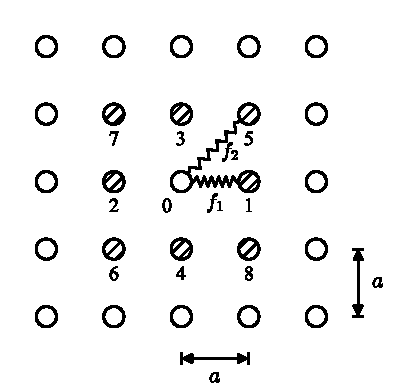
\includegraphics[width=6.5cm]{fig2-1.pdf}\\{\small 图 2.1\quad 二维正方晶格}
\end{minipage}
\end{center}

在此模型中的弹性力常数
\begin{equation}
  \Phi_{\alpha\beta}(l)=-f_l\varepsilon_{\alpha}(l)\varepsilon_{\beta}(l)
  \quad(l\neq0)
\end{equation}
其中$f_l=f_1\,(l=1,2,3,4)$，$f_l=f_2\,(l=5,6,7,8)$，$\varepsilon_{\alpha}(l)$代表沿$\boldsymbol{R}_l$方向单位矢在$\alpha$方向上的分量.对于中心原子的$\Phi_{\alpha\beta}(0)$可利用关系式(2.1.7)和(2.2.16)求得
\begin{equation}
  \Phi_{\alpha\beta}(0)=-\sum_{l\neq0}\Phi_{\alpha\beta}(l)
  =\sum_{l=1}^{8}f_l\varepsilon_l(l)\varepsilon_{\beta}(l)
\end{equation}
算出的$\Phi$矩阵为
\begin{equation}
\left.\begin{aligned}
  &\Phi(0)=2(f_1+f_2)\begin{pmatrix}1&0\\0&1\end{pmatrix}\\
  &\Phi(1)=\Phi(2)=-f_1\begin{pmatrix}1&0\\0&0\end{pmatrix},
  \quad\Phi(3)=\Phi(4)=-f_1\begin{pmatrix}0&0\\0&1\end{pmatrix}\\
  &\Phi(5)=\Phi(6)=-\frac{1}{2}f_2\begin{pmatrix}1&1\\1&1\end{pmatrix},
  \quad\Phi(7)=\Phi(8)=-\frac{1}{2}f_2\begin{pmatrix}1&-1\\-1&1\end{pmatrix}
\end{aligned}\right\}
\end{equation}
动力矩阵应由式(2.2.18)代入(2.2.3)作计算，求和限于最近邻及次近邻$(l=1,2,\cdots,8)$，即
\begin{equation}
  D(\boldsymbol{k})=\frac{2}{M}\left(\begin{array}{cc}
  \left[\begin{array}{l}f_1(1-\cos k_xa)+\\[0.3em]
  f_2(1-\cos k_xa\cos k_ya)\end{array}\right] & f_2\sin k_xa\sin k_ya\\[4ex]
  f_2\sin k_xa\sin k_ya &
  \left[\begin{array}{l}f_1(1-\cos k_ya)+\\[0.3em]
  f_2(1-\cos k_xa\cos k_ya)\end{array}\right]
  \end{array}\right)
\end{equation}
频率$\omega_{\sigma}(\boldsymbol{k})$由$D(\boldsymbol{k})$代入久期方程决定：
\begin{equation}
  \det\parallel D(\boldsymbol{k})-\omega^2I\parallel=0\,,
  \quad I=\begin{pmatrix}1&0\\0&1\end{pmatrix}
\end{equation}
根据式(2.2.19)，动力矩阵具有如下特性：
\begin{equation}
  D\Bigl(k_x+\frac{2\pi}{a},k_y+\frac{2\pi}{a}\Bigr)
  =D(k_x,k_y)=D(\boldsymbol{k})
\end{equation}
因此$\omega_{\sigma}(k_x,k_y)=\omega_{\sigma}\Bigl(k_x+\frac{2\pi}{a},k_y+\frac{2\pi}{a}\Bigr)$是倒点阵的周期函数，只需要在BZ中讨论格波.我们对于BZ中高对称点(线)上的$\omega_{\sigma}(\boldsymbol{k})$感兴趣，今分别求之：

(i)$\Sigma$线(包括$\Gamma$，M点)：令$k_x=k_y=k/\sqrt{2}$
\begin{equation}
\begin{aligned}
  \omega_1^2(\Sigma)&=\frac{2}{M}\bigg[f_1\bigg(1-\cos\frac{ka}{\sqrt{2}}\bigg)
  +f_2\bigl(1-\cos\sqrt{2}\,ka\bigr)\bigg]=\omega_{\mathrm{L}}^2(\Sigma)\\
  \omega_2^2(\Sigma)&=\frac{2}{M}f_1\bigg(1-\cos\frac{ka}{\sqrt{2}}\bigg)
  =\omega_{\mathrm{T}}^2(\Sigma)
\end{aligned}
\end{equation}
极化矢量可将以上结果代入式(2.1.13)求得
\begin{equation}
\left.\begin{aligned}
  &\boldsymbol{e}_{\Sigma1}=\Bigl(\frac{1}{\sqrt{2}},\frac{1}{\sqrt{2}}\Bigr)
  =\boldsymbol{e}_{\Sigma}^{\mathrm{L}}\\
  &\boldsymbol{e}_{\Sigma2}=\Bigl(-\frac{1}{\sqrt{2}},\frac{1}{\sqrt{2}}\Bigr)
  =\boldsymbol{e}_{\Sigma}^{\mathrm{T}}
\end{aligned}\right\}
\end{equation}
$\boldsymbol{e}_{\Sigma1}$与传播方向平行代表纵波$\boldsymbol{e}_{\Sigma}^{\mathrm{L}}$，$\boldsymbol{e}_{\Sigma2}$与传播方向相垂直为横波极化矢量$\boldsymbol{e}_{\Sigma}^{\mathrm{T}}$，如图2.2所标明.沿$\Sigma$的格波色散曲线如图2.3所示.当$4f_2>f_1$时纵波的$\omega$曲线在BZ内有极大点出现，这是与一维频谱不同之处.

\begin{center}
\begin{minipage}{6cm}
\centering
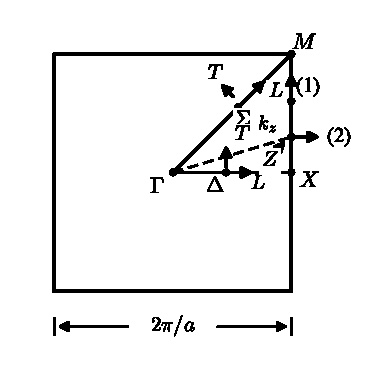
\includegraphics[width=6cm]{fig2-2.pdf}\\{\small 图 2.2\quad 二维正方晶格的极化矢量}
\end{minipage}
\end{center}

\begin{center}
\begin{minipage}{6cm}
\centering
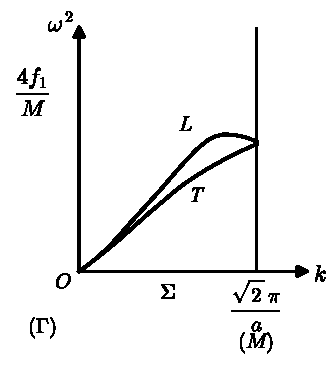
\includegraphics[width=6cm]{fig2-3.pdf}\\{\small 图 2.3}
\end{minipage}
\end{center}

(ii)$\Delta$线(包括$\Gamma$、X点)：令$k_x=k$，$k_y=0$
\begin{equation}
\begin{gathered}
  \omega_1^2(\Delta)=\frac{2}{M}(f_1+f_2)(1-\cos ka)=\omega_{\mathrm{L}}^2(\Delta)\\[1ex]
  \omega_2^2(\Delta)=\frac{2}{M}f_2(1-\cos ka)=\omega_{\mathrm{T}}^2(\Delta)
\end{gathered}
\end{equation}
\begin{equation}
  \boldsymbol{e}_{\Delta1}=(1,0)=\boldsymbol{e}_{\Delta}^{\mathrm{L}}\,,
  \quad\boldsymbol{e}_{\Delta2}=(0,1)=\boldsymbol{e}_{\Delta}^{\mathrm{T}}
\end{equation}
与$\Sigma$线相似，在$\Delta$线上纵波频率也高于横波，其色散曲线如图2.4.

(iii)Z线(包括X及M点)：令$k_x=\frac{\pi}{a}$，$k_y=k'$
\begin{equation}
\left.\begin{aligned}
  &\omega_1^2(Z)=\frac{2}{M}\bigl[2f_1+f_2(1+\cos k'a)\bigr]\\
  &\omega_2^2(Z)=\frac{2}{M}\bigl[f_1(1-\cos k'a)+f_2(1+\cos k'a)\bigr]
\end{aligned}\right\}
\end{equation}
相对应的极化矢量为
\begin{equation}
  \boldsymbol{e}_{Z1}=(0,1)\,,\quad\boldsymbol{e}_{Z2}=(1,0)
\end{equation}
它们与Z点的波矢方向($\Gamma$Z连线方向)既不平行，也不垂直.说明在Z线上的格波既非纵波，又非横波.因此，晶体中的格波只有沿某些高对称的$\boldsymbol{k}$方向传播时，才有纵横之分.这是晶体与各向同性连续介质不同之处.图2.5为沿Z方向的格波色散曲线.

从图2.3—图2.5可以看出BZ中只有在$\Gamma$与M点上纵波与横波的本征频率相同，这就是第一章§4所预言的简并情形.

\begin{center}
\begin{minipage}{6.5cm}
\centering
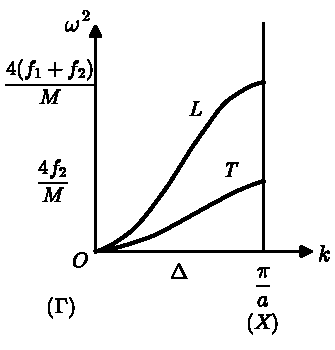
\includegraphics[width=6.5cm]{fig2-4.pdf}\\{\small 图 2.4}
\end{minipage}
\end{center}

\begin{center}
\begin{minipage}{6.5cm}
\centering
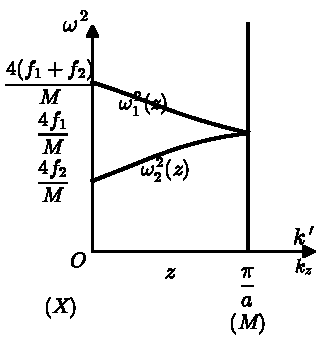
\includegraphics[width=6.5cm]{fig2-5.pdf}\\{\small 图 2.5}
\end{minipage}
\end{center}

为了熟悉复式晶格的动力矩阵$D(\boldsymbol{k})$、本征频率$\omega_{\sigma}(\boldsymbol{k})$和极化矢量$\boldsymbol{e}_{\boldsymbol{k}\sigma}(s)$的运算，我们将讨论一维复式晶格情况.

例如一维双原子链.模型如图2.6所示，两种原子$M_1$与$M_2$交替排列，近邻互作用的弹性恢复力常数分别为$f_1$和$f_2$，原胞中原子标号$s=1$，2.由于是一维，方向指标$(\alpha,\beta)$可略去.根据图中模型立刻求得$\Phi\binom{l-l'}{s,s'}$：
\begin{equation}
\left.\begin{aligned}
  &\Phi\binom{1}{1,2}=\Phi\binom{-1}{2,1}=-f_2\\
  &\Phi\binom{0}{1,2}=\Phi\binom{0}{2,1}=-f_1\\
  &\Phi\binom{0}{1,1}=-\Bigl[\Phi\binom{0}{1,2}+\Phi\binom{1}{1,2}\Bigr]
  =(f_1+f_2)=\Phi\binom{0}{2,2}
\end{aligned}\right\}
\end{equation}
其中$\Phi\binom{0}{s,s'}$利用了关系式(2.1.24)，计算准至最近邻互作用.

\begin{center}
\begin{minipage}{8cm}
\centering
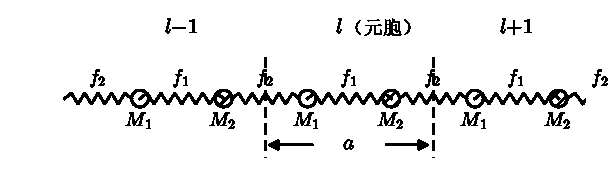
\includegraphics[width=8cm]{fig2-6.pdf}\\{\small 图 2.6\quad 一维复式晶格模型}
\end{minipage}
\end{center}

将(2.2.28)代入动力矩阵的公式(2.1.22)得到$D\binom{\boldsymbol{k}}{s,s'}\,(s,s'=1,2)$，它们组成二维矩阵
\begin{equation}
  D(\boldsymbol{k})=\left(\begin{array}{cc}
  D\binom{\boldsymbol{k}}{1,1} & D\binom{\boldsymbol{k}}{1,2}\\[1.5ex]
  D\binom{\boldsymbol{k}}{2,1} & D\binom{\boldsymbol{k}}{2,2}
  \end{array}\right)
  =\left(\begin{array}{cc}
  \dfrac{1}{M_1}(f_1+f_2) & -\dfrac{1}{\sqrt{M_1M_2}}\bigl(f_1+f_2\mathrm{e}^{-\mathrm{i}ka}\bigr)\\[3ex]
  -\dfrac{1}{\sqrt{M_1M_2}}\bigl(f_1+f_2\mathrm{e}^{\mathrm{i}ka}\bigr) & \dfrac{1}{M_2}(f_1+f_2)
  \end{array}\right)
\end{equation}
频率本征值由$\det\parallel D(\boldsymbol{k})-\omega^2I\parallel=0$决定，结果为
\begin{equation}
\begin{aligned}
  \omega_{\pm}^2(\boldsymbol{k})&=\frac{1}{2}(f_1+f_2)
  \left(\frac{1}{M_1}+\frac{1}{M_2}\right)\\
  &\quad\times\left[1\pm\sqrt{1-\frac{8f_1f_2M_1M_2}{(f_1+f_2)^2(M_1+M_2)^2}(1-\cos ka)}\,\right]
\end{aligned}
\end{equation}
有两支频谱$\omega_{\pm}^2(\boldsymbol{k})$，其中由于$\omega_-(\boldsymbol{k}=0)=0$，因此$\omega_-$就是固体物理学中的声频支格波，简称声学模，而$\omega_+$则代表光频支格波(光学模)，两支格波的色散曲线分别绘于图2.7中.

\begin{center}
\begin{minipage}{7cm}
\centering
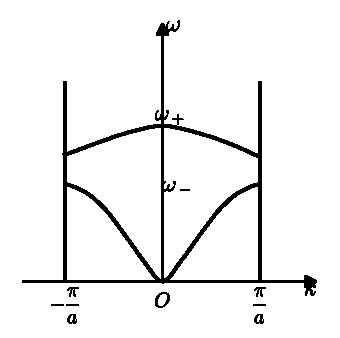
\includegraphics[width=7cm]{fig2-7.pdf}\\{\small 图 2.7}
\end{minipage}
\end{center}

$\boldsymbol{k}=0$时动力矩阵为实对称矩阵
\begin{equation}
\begin{gathered}
  D\binom{0}{1,1}=\frac{1}{M_1}(f_1+f_2)\\[1ex]
  D\binom{0}{2,2}=\frac{1}{M_2}(f_1+f_2)\\[1ex]
  D\binom{0}{1,2}=D\binom{0}{2,1}
  =-\frac{1}{\sqrt{M_1M_2}}(f_1+f_2)
\end{gathered}
\end{equation}
极化矢量$\boldsymbol{e}_{\sigma}(s)\,(\sigma=\pm\,,s=1,2)$可由式(2.1.20)决定，它们也是实量
\begin{equation}
  \boldsymbol{e}_{+}(1)=-\sqrt{\frac{M_2}{M_1}}\boldsymbol{e}_{+}(2)\,,
  \quad\boldsymbol{e}_{-}(1)=\sqrt{\frac{M_1}{M_2}}\boldsymbol{e}_{-}(2)
\end{equation}
显然，光频支振动代表元胞内$M_1$与$M_2$两原子的相对运动，其极化矢量异号，而声频支振动中两原子极化矢量同号，为同向运动，与前面的一般性讨论相符.再利用$\boldsymbol{e}_{\pm}(s)$的归一条件(2.1.27)
\begin{equation}
  e_{\pm}^2(1)+e_{\pm}^2(2)=1
\end{equation}
最后求得$\boldsymbol{k}=0$时声、光频支的极化矢量
\begin{equation}
\begin{gathered}
  \boldsymbol{e}_{+}(1)=-\frac{1}{\sqrt{\Bigl(1+\dfrac{M_1}{M_2}\Bigr)}}\,,
  \quad\boldsymbol{e}_{+}(2)=\frac{1}{\sqrt{\Bigl(1+\dfrac{M_2}{M_1}\Bigr)}}\\[3ex]
  \boldsymbol{e}_{-}(1)=\frac{1}{\sqrt{\Bigl(1+\dfrac{M_2}{M_1}\Bigr)}}\,,
  \quad\boldsymbol{e}_{-}(2)=\frac{1}{\sqrt{\Bigl(1+\dfrac{M_1}{M_2}\Bigr)}}
\end{gathered}
\end{equation}

\section{简正坐标}

在简谐近似下晶格振动已由简正模的线性叠加表示，按照式(2.1.19)其矢量形式为
\begin{equation}
  \boldsymbol{u}_l=(NM)^{-\frac{1}{2}}\sum_{\boldsymbol{k},\sigma}
  Q_{\boldsymbol{k}\sigma}\boldsymbol{e}_{\boldsymbol{k}\sigma}
  \mathrm{e}^{\mathrm{i}\boldsymbol{k}\cdot\boldsymbol{R}_l}
\end{equation}
其中$Q_{\boldsymbol{k}\sigma}$是复简正坐标，而位移$u_l^{\alpha}$为实量，这里存在一个附加条件
\begin{equation}
  \boldsymbol{e}_{\boldsymbol{k}\sigma}Q_{\boldsymbol{k}\sigma}^{*}
  =\boldsymbol{e}_{-\boldsymbol{k}\sigma}Q_{-\boldsymbol{k}\sigma}
\end{equation}
若约定极化矢量满足关系式\footnote{也可以约定$\boldsymbol{e}_{\boldsymbol{k}\sigma}=-\boldsymbol{e}_{-\boldsymbol{k}\sigma}$，则$Q_{\boldsymbol{k}\sigma}^{*}=-Q_{-\boldsymbol{k}\sigma}$，其结果相同.}
\begin{equation}
  \boldsymbol{e}_{\boldsymbol{k}\sigma}=\boldsymbol{e}_{-\boldsymbol{k}\sigma}
\end{equation}
则复简正坐标
\begin{equation}
  Q_{\boldsymbol{k}\sigma}^{*}=Q_{-\boldsymbol{k}\sigma}
\end{equation}
在简单晶体中，晶格振动的哈密顿量(2.1.8)仍为各原子位移的耦合形式，我们希望将$H$表示成各独立项相加.为此，首先用(2.3.1)将哈密顿量变换为简正坐标表示.对于动能
\begin{equation}
\begin{aligned}
  T&=\frac{1}{2}\sum_l M\dot{\boldsymbol{u}}_l\cdot\dot{\boldsymbol{u}}_l\\
  &=\frac{1}{2}\sum_{\boldsymbol{k},\boldsymbol{k}'}\sum_{\sigma,\sigma'}
  \dot{Q}_{\boldsymbol{k}'\sigma'}\dot{Q}_{\boldsymbol{k}\sigma}
  (\boldsymbol{e}_{\boldsymbol{k}'\sigma'}\cdot\boldsymbol{e}_{\boldsymbol{k}\sigma})
  \delta_{\boldsymbol{k}',-\boldsymbol{k}}\\
  &=\frac{1}{2}\sum_{\boldsymbol{k},\sigma}\sum_{\sigma'}
  \dot{Q}_{\boldsymbol{k}\sigma'}^{*}\dot{Q}_{\boldsymbol{k}\sigma}
  (\boldsymbol{e}_{\boldsymbol{k}\sigma'}\cdot\boldsymbol{e}_{\boldsymbol{k}\sigma})\\
  &=\frac{1}{2}\sum_{\boldsymbol{k},\sigma}\dot{Q}_{\boldsymbol{k}\sigma}^{*}\dot{Q}_{\boldsymbol{k}\sigma}
\end{aligned}
\end{equation}
其中利用了约定关系式(2.3.3)与(2.3.4)，本征矢量的正交关系式(2.1.16)以及当波矢限于BZ内时的关系式
\begin{equation*}
  \frac{1}{N}\sum_l\mathrm{e}^{\mathrm{i}(\boldsymbol{k}-\boldsymbol{k}')\cdot\boldsymbol{R}_l}
  =\delta_{\boldsymbol{k}'\boldsymbol{k}}
\end{equation*}
晶格振动势能在简谐近似下为
\begin{equation}
\begin{aligned}
  \Delta\Phi&=\frac{1}{2}\sum_{l,l'}\sum_{\alpha,\beta}
  u_l^{\alpha}\Phi_{\alpha\beta}(l-l')u_{l'}^{\beta}\\
  &=\frac{1}{2}\sum_{\boldsymbol{k},\boldsymbol{k}'}\sum_{\sigma,\sigma'}
  Q_{\boldsymbol{k}\sigma}^{*}Q_{\boldsymbol{k}'\sigma'}
  \frac{1}{N}\sum_l\mathrm{e}^{\mathrm{i}(\boldsymbol{k}'-\boldsymbol{k})\cdot\boldsymbol{R}_l}A
\end{aligned}
\end{equation}
其中
\begin{equation*}
\begin{aligned}
  A&=\sum_{\alpha}e_{\boldsymbol{k}\sigma}^{\alpha}\sum_{\beta}
  \Bigl\{\frac{1}{M}\sum_l\Phi_{\alpha\beta}(l-l')
  \mathrm{e}^{-\mathrm{i}\boldsymbol{k}'\cdot(\boldsymbol{R}_l-\boldsymbol{R}_{l'})}\Bigr\}
  e_{\boldsymbol{k}'\sigma'}^{\beta}\\
  &=\sum_{\alpha}e_{\boldsymbol{k}\sigma}^{\alpha}\sum_{\beta}
  D_{\alpha\beta}(\boldsymbol{k}')e_{\boldsymbol{k}'\sigma'}^{\beta}\\
  &=\Bigl(\sum_{\alpha}e_{\boldsymbol{k}\sigma}^{\alpha}e_{\boldsymbol{k}'\sigma'}^{\alpha}\Bigr)
  \omega_{\sigma'}^2(\boldsymbol{k}')
\end{aligned}
\end{equation*}
这里利用了式(2.1.12)和对角化条件式(2.1.13).将$A$代入式(2.3.6)，再利用$\boldsymbol{e}_{\boldsymbol{k}\sigma}$的正交关系式(2.1.16)，得
\begin{equation}
  \Delta\Phi=\frac{1}{2}\sum_{\boldsymbol{k},\sigma}
  \omega_{\sigma}^2(\boldsymbol{k})Q_{\boldsymbol{k}\sigma}^{*}Q_{\boldsymbol{k}\sigma}
\end{equation}
晶格振动的哈密顿量简化为
\begin{equation*}
  H=\frac{1}{2}\sum_{\boldsymbol{k},\sigma}\Bigl\{\dot{Q}_{\boldsymbol{k}\sigma}^{*}\dot{Q}_{\boldsymbol{k}\sigma}
  +\omega_{\sigma}^2(\boldsymbol{k})Q_{\boldsymbol{k}\sigma}^{*}Q_{\boldsymbol{k}\sigma}\Bigr\}
\end{equation*}
$H$在简正坐标中表示为$3N$个独立项之和，利用拉氏函数$L=T-\Delta\Phi$可求出$Q_{\boldsymbol{k}\sigma}$的共轭动量$P_{\boldsymbol{k}\sigma}$
\begin{equation}
  P_{\boldsymbol{k}\sigma}=\frac{\partial L}{\partial\dot{Q}_{\boldsymbol{k}\sigma}}
  =\dot{Q}_{\boldsymbol{k}\sigma}^{*}
\end{equation}
\begin{equation}
  H=\frac{1}{2}\sum_{\boldsymbol{k},\sigma}\Bigl\{P_{\boldsymbol{k}\sigma}^{*}P_{\boldsymbol{k}\sigma}
  +\omega_{\sigma}^2(\boldsymbol{k})Q_{\boldsymbol{k}\sigma}^{*}Q_{\boldsymbol{k}\sigma}\Bigr\}
\end{equation}
根据正则方程
\begin{equation*}
  \dot{P}_{\boldsymbol{k}\sigma}=-\frac{\partial H}{\partial Q_{\boldsymbol{k}\sigma}}
\end{equation*}
可求出简正坐标$Q_{\boldsymbol{k}\sigma}$满足方程：
\begin{equation}
  \ddot{Q}_{\boldsymbol{k}\sigma}+\omega_{\sigma}^2(\boldsymbol{k})Q_{\boldsymbol{k}\sigma}=0
\end{equation}
与简谐振子的运动方程在形式上相同，利用正交条件作式(2.3.1)的逆傅里叶变换求得简正坐标
\begin{equation}
\begin{aligned}
  Q_{\boldsymbol{k}\sigma}&=\sqrt{\frac{M}{N}}\sum_l
  (\boldsymbol{e}_{\boldsymbol{k}\sigma}\cdot\boldsymbol{u}_l)
  \mathrm{e}^{-\mathrm{i}\boldsymbol{k}\cdot\boldsymbol{R}_l}\\
  &=\frac{1}{\sqrt{NM}}\sum_{l,\alpha}Me_{\boldsymbol{k}\sigma}^{\alpha *}
  u_l^{\alpha}\mathrm{e}^{-\mathrm{i}\boldsymbol{k}\cdot\boldsymbol{R}_l}
\end{aligned}
\end{equation}
显然，$Q_{\boldsymbol{k}\sigma}$代表$N$个原子的集体振动，简正坐标是集体坐标.简正坐标$Q_{\boldsymbol{k}\sigma}$的共轭动量$P_{\boldsymbol{k}\sigma}$与第$l$个原子位移的共轭动量$\boldsymbol{p}_l=M\dot{\boldsymbol{u}}_l$之间有类似的变换关系：
\begin{equation}
  \boldsymbol{p}_l=M\dot{\boldsymbol{u}}_l=\sqrt{\frac{M}{N}}
  \sum_{\boldsymbol{k},\sigma}P_{\boldsymbol{k}\sigma}\boldsymbol{e}_{\boldsymbol{k}\sigma}
  \mathrm{e}^{-\mathrm{i}\boldsymbol{k}\cdot\boldsymbol{R}_l}
\end{equation}
其逆变换为
\begin{equation}
\begin{aligned}
  P_{\boldsymbol{k}\sigma}&=\frac{1}{\sqrt{NM}}\sum_l
  (\boldsymbol{e}_{\boldsymbol{k}\sigma}\cdot\boldsymbol{p}_l)
  \mathrm{e}^{\mathrm{i}\boldsymbol{k}\cdot\boldsymbol{R}_l}\\
  &=\frac{1}{\sqrt{NM}}\sum_{l,\alpha}e_{\boldsymbol{k}\sigma}^{\alpha *}
  p_l^{\alpha}\mathrm{e}^{\mathrm{i}\boldsymbol{k}\cdot\boldsymbol{R}_l}
\end{aligned}
\end{equation}
表明$P_{\boldsymbol{k}\sigma}$也是集体坐标.

\section{声子}

晶格振动必须用量子力学处理，其量子化条件为共轭量$p_l^{\alpha}$，$u_l^{\beta}$满足对易式
\begin{equation}
\left.\begin{aligned}
  &\bigl[p_l^{\alpha},u_{l'}^{\beta}\bigr]\equiv p_l^{\alpha}u_{l'}^{\beta}
  -u_{l'}^{\beta}p_l^{\alpha}=\frac{\hbar}{\mathrm{i}}\delta_{\alpha\beta}\delta_{ll'}\\
  &\bigl[u_l^{\alpha},u_{l'}^{\beta}\bigr]
  =\bigl[p_l^{\alpha},p_{l'}^{\beta}\bigr]=0\quad(\alpha,\beta=x,y,z)
\end{aligned}\right\}
\end{equation}
利用变换关系式(2.3.11)、(2.3.13)以及正交关系式(2.1.16)，容易由式(2.4.1)求得简正坐标$P_{\boldsymbol{k}\sigma}$、$Q_{\boldsymbol{k}\sigma}$的对易律
\begin{equation}
\left.\begin{aligned}
  [P_{\boldsymbol{k}\sigma},Q_{\boldsymbol{k}'\sigma'}]
  &=\frac{1}{N}\sum_{l,l'}\sum_{\alpha,\beta}
  \bigl(e_{\boldsymbol{k}\sigma}^{\alpha *}e_{\boldsymbol{k}'\sigma'}^{\beta}\bigr)
  \bigl[p_l^{\alpha},u_{l'}^{\beta}\bigr]
  \mathrm{e}^{\mathrm{i}(\boldsymbol{k}\cdot\boldsymbol{R}_l-\boldsymbol{k}'\cdot\boldsymbol{R}_{l'})}\\
  &=\frac{\hbar}{\mathrm{i}}\sum_{\alpha}
  \bigl(e_{\boldsymbol{k}\sigma}^{\alpha *}e_{\boldsymbol{k}'\sigma'}^{\alpha}\bigr)
  \frac{1}{N}\sum_l\mathrm{e}^{\mathrm{i}(\boldsymbol{k}-\boldsymbol{k}')\cdot\boldsymbol{R}_l}\\
  &=\frac{\hbar}{\mathrm{i}}\delta_{\sigma\sigma'}\delta_{\boldsymbol{k}\boldsymbol{k}'}\\
  [Q_{\boldsymbol{k}\sigma},Q_{\boldsymbol{k}'\sigma'}]
  &=[P_{\boldsymbol{k}\sigma},P_{\boldsymbol{k}'\sigma'}]=0
\end{aligned}\right\}
\end{equation}
应当指出在$H$的复简正坐标表式(2.3.9)中，每个单项$\frac{1}{2}\bigl\{P_{\boldsymbol{k}\sigma}^{*}P_{\boldsymbol{k}\sigma}+\omega_{\sigma}^2(\boldsymbol{k})Q_{\boldsymbol{k}\sigma}^{*}Q_{\boldsymbol{k}\sigma}\bigr\}$并不对应于量子力学中频率为$\omega_{\sigma}(\boldsymbol{k})$的简谐振子哈密顿量$\frac{1}{2}\{p^2+\omega^2q^2\}$，因为$(P,Q)$为复共轭量，而$(p,q)$为实量.根据式(2.3.4)与(2.3.8)还可以看出，式(2.3.9)实际上是
\begin{equation}
  H=\frac{1}{2}\sum_{\boldsymbol{k},\sigma}\bigl\{P_{-\boldsymbol{k}\sigma}P_{\boldsymbol{k}\sigma}
  +\omega_{\sigma}^2(\boldsymbol{k})Q_{-\boldsymbol{k}\sigma}Q_{\boldsymbol{k}\sigma}\bigr\}
\end{equation}
其中$\boldsymbol{k}$与$-\boldsymbol{k}$项仍然混杂.为消除$H$中$\boldsymbol{k}$与$-\boldsymbol{k}$的交叉项，通过正则变换定义新算符
\begin{equation}
\left.\begin{aligned}
  a_{\boldsymbol{k}\sigma}&=\sqrt{\frac{\omega_{\sigma}(\boldsymbol{k})}{2\hbar}}
  \left(Q_{\boldsymbol{k}\sigma}-\frac{P_{-\boldsymbol{k}\sigma}}{\mathrm{i}\omega_{\sigma}(\boldsymbol{k})}\right)\\[1ex]
  a_{\boldsymbol{k}\sigma}^{+}&=\sqrt{\frac{\omega_{\sigma}(\boldsymbol{k})}{2\hbar}}
  \left(Q_{-\boldsymbol{k}\sigma}+\frac{P_{\boldsymbol{k}\sigma}}{\mathrm{i}\omega_{\sigma}(\boldsymbol{k})}\right)
\end{aligned}\right\}
\end{equation}
不难验证
\begin{equation*}
\begin{aligned}
  \sum_{\boldsymbol{k},\sigma}\hbar\omega_{\sigma}(\boldsymbol{k})a_{\boldsymbol{k}\sigma}^{+}a_{\boldsymbol{k}\sigma}
  &=\frac{1}{2}\sum_{\boldsymbol{k},\sigma}\bigl\{P_{-\boldsymbol{k}\sigma}P_{\boldsymbol{k}\sigma}
  +\omega_{\sigma}^2(\boldsymbol{k})Q_{-\boldsymbol{k}\sigma}Q_{\boldsymbol{k}\sigma}\bigr\}\\
  &\quad-\mathrm{i}\frac{1}{2}\sum_{\boldsymbol{k},\sigma}\omega_{\sigma}(\boldsymbol{k})
  \bigl[P_{\boldsymbol{k}\sigma},Q_{\boldsymbol{k}\sigma}\bigr]\\
  &=H-\frac{1}{2}\sum_{\boldsymbol{k},\sigma}\hbar\omega_{\sigma}(\boldsymbol{k})
\end{aligned}
\end{equation*}
推导时只用了对易式(2.4.2)与频率的普遍关系式$\omega_{\sigma}(\boldsymbol{k})=\omega_{\sigma}(-\boldsymbol{k})$.用新算符$a_{\boldsymbol{k}\sigma}$表示的$H$为下列不含$\boldsymbol{k}$与$-\boldsymbol{k}$交叉项的对角形式
\begin{equation}
  H=\sum_{\boldsymbol{k},\sigma}\left(a_{\boldsymbol{k}\sigma}^{+}a_{\boldsymbol{k}\sigma}
  +\frac{1}{2}\right)\hbar\omega_{\sigma}(\boldsymbol{k})
  =\sum_{\boldsymbol{k},\sigma}H_{\boldsymbol{k}\sigma}
\end{equation}
对易关系为
\begin{equation}
\begin{aligned}
  &\bigl[a_{\boldsymbol{k}\sigma},a_{\boldsymbol{k}'\sigma'}^{+}\bigr]
  =\delta_{\sigma\sigma'}\delta_{\boldsymbol{k}\boldsymbol{k}'}\\
  &\bigl[a_{\boldsymbol{k}\sigma},a_{\boldsymbol{k}'\sigma'}\bigr]
  =\bigl[a_{\boldsymbol{k}\sigma}^{+},a_{\boldsymbol{k}'\sigma'}^{+}\bigr]=0
\end{aligned}
\end{equation}
用$a_{\boldsymbol{k}\sigma}$及$a_{\boldsymbol{k}\sigma}^{+}$表示的位移得
\begin{equation}
  \boldsymbol{u}_l=\sum_{\boldsymbol{k},\sigma}
  \left(\frac{\hbar}{2NM\omega_{\sigma}(\boldsymbol{k})}\right)^{\frac{1}{2}}
  \boldsymbol{e}_{\boldsymbol{k}\sigma}
  \bigl\{a_{\boldsymbol{k}\sigma}\mathrm{e}^{\mathrm{i}\boldsymbol{k}\cdot\boldsymbol{R}_l}
  +a_{\boldsymbol{k}\sigma}^{+}\mathrm{e}^{-\mathrm{i}\boldsymbol{k}\cdot\boldsymbol{R}_l}\bigr\}
\end{equation}
其时间依赖关系可利用海森伯运动方程
\begin{equation*}
\begin{aligned}
  \dot{a}_{\boldsymbol{k}\sigma}&=\frac{\mathrm{i}}{\hbar}[H,a_{\boldsymbol{k}\sigma}]
  =-\mathrm{i}\omega_{\sigma}(\boldsymbol{k})a_{\boldsymbol{k}\sigma}\\
  a_{\boldsymbol{k}\sigma}&=a_{\boldsymbol{k}}(0)\mathrm{e}^{-\mathrm{i}\omega_{\sigma}(\boldsymbol{k})t}
\end{aligned}
\end{equation*}
代入式(2.4.7)，得
\begin{equation*}
\begin{aligned}
  \boldsymbol{u}_l(t)&=\sum_{\boldsymbol{k},\sigma}
  \left(\frac{\hbar}{2NM\omega_{\sigma}(\boldsymbol{k})}\right)^{\frac{1}{2}}
  \boldsymbol{e}_{\boldsymbol{k}\sigma}
  \bigl\{a_{\boldsymbol{k}\sigma}(0)
  \mathrm{e}^{\mathrm{i}[\boldsymbol{k}\cdot\boldsymbol{R}_l-\omega_{\sigma}(\boldsymbol{k})t]}\\
  &\quad+a_{\boldsymbol{k}\sigma}^{+}(0)
  \mathrm{e}^{-\mathrm{i}[\boldsymbol{k}\cdot\boldsymbol{R}_l-\omega_{\sigma}(\boldsymbol{k})t]}\bigr\}\\
  &=\sum_{\boldsymbol{k},\sigma}
  \left(\frac{\hbar}{2NM\omega_{\sigma}(\boldsymbol{k})}\right)^{\frac{1}{2}}
  \boldsymbol{e}_{\boldsymbol{k}\sigma}\bigl\{a_{\boldsymbol{k}\sigma}(0)
  \mathrm{e}^{\mathrm{i}[\boldsymbol{k}\cdot\boldsymbol{R}_l-\omega_{\sigma}(\boldsymbol{k})t]}
  +\mathrm{h.c.}\bigr\}
\end{aligned}
\end{equation*}
其中h.c.代表厄米共轭项.这是位移的行波展式，其中每一求和项代表频率$\omega_{\sigma}(\boldsymbol{k})$、偏振$\boldsymbol{e}_{\boldsymbol{k}\sigma}$、沿$\boldsymbol{k}$方向传播的格波，它所对应的哈密顿量是$H_{\boldsymbol{k}\sigma}$.不难证明，定态薛定谔方程
\begin{equation}
  H_{\boldsymbol{k}\sigma}\psi_{\boldsymbol{k}\sigma}
  =\varepsilon_{\boldsymbol{k}\sigma}\psi_{\boldsymbol{k}\sigma}\,,
  \quad H_{\boldsymbol{k}\sigma}\equiv
  \left(a_{\boldsymbol{k}\sigma}^{+}a_{\boldsymbol{k}\sigma}+\frac{1}{2}\right)
  \hbar\omega_{\sigma}(\boldsymbol{k})
\end{equation}
的解$\varepsilon_{\boldsymbol{k}\sigma}$与频率为$\omega_{\sigma}(\boldsymbol{k})$的简谐振子能量形式相同.式(2.4.8)可等效地写为
\begin{equation}
  \hbar\omega_{\sigma}(\boldsymbol{k})a_{\boldsymbol{k}\sigma}^{+}a_{\boldsymbol{k}\sigma}
  \psi_{\boldsymbol{k}\sigma}
  =\Bigl[\varepsilon_{\boldsymbol{k}\sigma}
  -\frac{1}{2}\hbar\omega_{\sigma}(\boldsymbol{k})\Bigr]\psi_{\boldsymbol{k}\sigma}
  \equiv\varepsilon'_{\boldsymbol{k}\sigma}\psi_{\boldsymbol{k}\sigma}
\end{equation}
为书写简便起见，暂略去脚标$(\boldsymbol{k},\sigma)$，将上式写成
\begin{equation}
  \hbar\omega a^{+}a\psi=\varepsilon'\psi
\end{equation}
下面分别讨论算符方程式(2.4.10)的基态和激发态：

\subsection*{(i) 基态}

设基态为$\psi_0$，有能量$\varepsilon'_0$，它应当是具有最低能量的状态，采用狄拉克(Dirac)符号，用$\lvert0\rangle$表示$\psi_0$，则有等式
\begin{equation}
  \hbar\omega a^{+}a\lvert0\rangle=\varepsilon'_0\lvert0\rangle
\end{equation}
将算符$a$作用于此等式两边，并利用对易式(2.4.6)
\begin{equation*}
  \hbar\omega aa^{+}a\lvert0\rangle
  =\hbar\omega\bigl(a^{+}a+1\bigr)a\lvert0\rangle
  =\varepsilon'_0a\lvert0\rangle
\end{equation*}
得到另一个状态$a\lvert0\rangle$满足
\begin{equation*}
  \hbar\omega a^{+}a\bigl(a\lvert0\rangle\bigr)
  =(\varepsilon'_0-\hbar\omega)\bigl(a\lvert0\rangle\bigr)
\end{equation*}
当$\omega>0$时它比$\lvert0\rangle$态具有更低能量，显然与原假设矛盾.所以，基态必需满足条件
\begin{equation}
  a\lvert0\rangle=0
\end{equation}
上式即二次量子化表象中的基态定义.由此可知$a^{+}a\lvert0\rangle=0$，代入式(2.4.11)得$\varepsilon'_0=0$，于是基态能
\begin{equation}
  \varepsilon_0=\frac{1}{2}\hbar\omega
\end{equation}
它相当于振子的零点能.

\subsection*{(ii) 激发态}

用算符$a^{+}$作用于基态，再利用对易关系，可求出等式
\begin{equation}
  \hbar\omega a^{+}a\bigl(a^{+}\lvert0\rangle\bigr)
  =\hbar\omega\bigl(a^{+}\lvert0\rangle\bigr)
\end{equation}
$a^{+}\lvert0\rangle$代表激发一个格波量子$\hbar\omega$的状态，称为第一激发态.若用$(a^{+})^n$作用，则得到
\begin{equation*}
  \hbar\omega a^{+}a\bigl\{(a^{+})^n\lvert0\rangle\bigr\}
  =n\hbar\omega\bigl\{(a^{+})^n\lvert0\rangle\bigr\}
\end{equation*}
因此$(a^{+})^n\lvert0\rangle$代表激发$n$个格波量子的状态，叫做第$n$激发态，并采用记号$\lvert n\rangle$表示
\begin{equation}
  \lvert n\rangle=c_n(a^{+})^n\lvert0\rangle
\end{equation}
其中$c_n$由归一条件决定.这样就得到式(2.4.10)的解为
\begin{equation*}
\begin{gathered}
  \hbar\omega a^{+}a\lvert n\rangle=\varepsilon'_n\lvert n\rangle\\[1ex]
  \varepsilon'_n=n\hbar\omega\quad(n=1,2,3,\cdots)
\end{gathered}
\end{equation*}
由此可见，格波能量总是以量子$\hbar\omega$一份份地激发，这个量子称为声子.激发了$n$个声子的$\omega$格波能量为
\begin{equation}
  \varepsilon_n=\varepsilon'_n+\frac{1}{2}\hbar\omega
  =\left(n+\frac{1}{2}\right)\hbar\omega
\end{equation}
与谐振子的能量一致.

\subsection*{(iii) 递推关系}

根据式(2.4.15)，可令
\begin{equation*}
  \lvert n\rangle=\lambda_na^{+}\lvert n-1\rangle
\end{equation*}
则求得
\begin{equation*}
\begin{aligned}
  \langle n\vert n\rangle&=|\lambda_n|^2\langle n-1\vert
  \bigl(aa^{+}\bigr)\vert n-1\rangle\\
  &=|\lambda_n|^2n\langle n-1\vert n-1\rangle
\end{aligned}
\end{equation*}
由于$\lvert n\rangle$与$\lvert n-1\rangle$都应当满足归一条件
\begin{equation*}
  \langle n\vert n\rangle=1\,,\quad\langle n-1\vert n-1\rangle=1
\end{equation*}
因此
\begin{equation*}
  \lambda_n=n^{-\frac{1}{2}}
\end{equation*}
并求出递推公式
\begin{equation}
  \lvert n\rangle=n^{-\frac{1}{2}}a^{+}\lvert n-1\rangle
\end{equation}
从递推公式(2.4.17)即可导出重要关系式
\begin{equation}
\left.\begin{aligned}
  &a^{+}\lvert n\rangle=\sqrt{n+1}\,\lvert n+1\rangle\\
  &a\lvert n\rangle=\sqrt{n}\,\lvert n-1\rangle
\end{aligned}\right\}
\end{equation}
上式说明$a^{+}$代表声子的产生算符，它使格波从$n$个声子态变为$(n+1)$个声子状态，而$a$算符使格波从$n$变为$(n-1)$个声子的状态，称为声子的消灭算符.算符
\begin{equation}
  \hat{n}\equiv a^{+}a
\end{equation}
有特性
\begin{equation}
  \hat{n}\lvert n\rangle=a^{+}a\lvert n\rangle=n\lvert n\rangle
  \quad(n=0,1,2,\cdots)
\end{equation}
其本征值为$n$，代表声子数，因此$\hat{n}$称为声子数算符.

以上讨论的优点是，无需具体给出$\lvert0\rangle$的表示式，就可以求得格波激发态的全部信息.$\lvert n\rangle$是用声子数算符本征值标记的状态，它就是希尔伯特空间中的态向量.

利用递推公式还可定出
\begin{equation}
\begin{gathered}
  c_n=\lambda_1\cdot\lambda_2\cdots\lambda_n=(n!)^{-\frac{1}{2}}\\[1ex]
  \lvert n\rangle=\frac{1}{\sqrt{n!}}(a^{+})^n\lvert0\rangle
\end{gathered}
\end{equation}
现在恢复脚标$(\boldsymbol{k},\sigma)$，讨论总哈密顿量$H$的本征能量.由于$k\sigma$格波的哈密顿量为$H_{\boldsymbol{k}\sigma}=\left(a_{\boldsymbol{k}\sigma}^{+}a_{\boldsymbol{k}\sigma}+\frac{1}{2}\right)\allowbreak\hbar\omega_{\sigma}(\boldsymbol{k})$，当状态用声子数标记为$\lvert n_{\boldsymbol{k}\sigma}\rangle$时，有能量$\varepsilon_{\boldsymbol{k}\sigma}=\left(n_{\boldsymbol{k}\sigma}+\frac{1}{2}\right)\hbar\omega_{\sigma}(\boldsymbol{k})$.因此
\begin{equation}
  H=\sum_{\boldsymbol{k},\sigma}H_{\boldsymbol{k}\sigma}
  =\sum_{\boldsymbol{k},\sigma}\left(a_{\boldsymbol{k}\sigma}^{+}a_{\boldsymbol{k}\sigma}
  +\frac{1}{2}\right)\hbar\omega_{\sigma}(\boldsymbol{k})
\end{equation}
代表$3N$种不同$(\boldsymbol{k},\sigma)$的无互作用声子系统，而总能量为
\begin{equation}
  E=\sum_{\boldsymbol{k},\sigma}\hbar\omega_{\sigma}(\boldsymbol{k})
  \left(n_{\boldsymbol{k}\sigma}+\frac{1}{2}\right)
\end{equation}
说明晶格振动的激发状态，在物理上可以用$3N$个独立格波的声子数组态$\lvert\{n_{\boldsymbol{k}\sigma}\}\rangle$表示.由于声子算符满足玻色对易式(2.4.6)，它是玻色粒子.式(2.4.22)与(2.4.23)代表理想玻色气体的$H$和$E$.这样，$N$个原子(离子)的耦合振荡问题在简谐近似下约化为独立玻色子系统.温度为$T$时，$(k\sigma)$格波所激发的平均声子数按玻色统计为
\begin{equation}
  \bar{n}_{\boldsymbol{k}\sigma}
  =\frac{1}{\exp\bigl[\hbar\omega_{\sigma}(\boldsymbol{k})/k_{\mathrm{B}}T\bigr]-1}
\end{equation}
当$T=0\,$K时，所有$(\boldsymbol{k},\sigma)$态上的声子数均为零，称为声子的真空，这时只有晶格振动的零点能.引入声子概念便于处理固体中相互作用问题，例如在声子-声子、电子-声子、光子-声子等互作用过程中，把声子当作有能量$\hbar\omega_{\sigma}(\boldsymbol{k})$和动量$\hbar\boldsymbol{k}$的玻色粒子来处理，将是十分方便的.但是，应当明白声子并不是一个真正的粒子，声子可以产生和消灭，有相互作用时声子数不守恒，声子动量的守恒律也不同于一般粒子，并且声子不能脱离固体存在.声子只是格波激发的量子，在多体理论中称为集体振荡的元激发或准粒子.

\section{长波方法(一)——声学模}

在多数问题中，长波长的声子起重要作用.为此，有必要单独讨论晶格动力学理论的长波极限$(\boldsymbol{k}\to0)$情况.由于声频支代表同一元胞中诸原子(基元)的质心运动，因此复式晶格中声学模也可以当简单晶格处理，只需认为$M$是元胞中原子的总质量.

对于长波长的晶格振动，其振幅在元胞间缓慢变化，晶体结构的原子性对问题影响不大，可以过渡到连续介质模型.

引入一个在空间缓变的位移场$\boldsymbol{u}(\boldsymbol{r})$代表$\boldsymbol{r}$点附近小体元的位移.当$\boldsymbol{r}=\boldsymbol{R}_l$(简记为$r=l$)时，$\boldsymbol{u}$就是$l$元胞中质心的位移
\begin{equation}
  u_l^{\alpha}=u^{\alpha}(\boldsymbol{r})\big|_{r=l}
\end{equation}
$\boldsymbol{u}$当然也是时间$t$的函数，而无需标明.考虑到振幅$u_l^{\alpha}$在元胞间缓慢变化，可将位移场作泰勒展开得到近似式
\begin{equation}
  u_{l'}^{\alpha}=u_l^{\alpha}
  +\sum_{\mu}\bigl(\boldsymbol{R}_{l'}-\boldsymbol{R}_l\bigr)_{\mu}
  \frac{\partial u^{\alpha}(\boldsymbol{r})}{\partial r_{\mu}}\bigg|_{r=l}
\end{equation}
式(2.5.1)与(2.5.2)是过渡到连续介质模型的基本关系式，此外还需定义密度
\begin{equation}
  \rho=\frac{M}{\Omega}
\end{equation}
和利用求和与积分的变换
\begin{equation}
  \Omega\sum_l\left(\cdots\right)=\int\mathrm{d}\tau\left(\cdots\right)
\end{equation}
可把晶格振动的动能按照式(2.5.1)与(2.5.4)改写为
\begin{equation*}
\begin{aligned}
  T&=\frac{1}{2}\sum_l M|\dot{\boldsymbol{u}}_l|^2\\
  &=\Omega\sum_l\frac{1}{2}\rho|\dot{\boldsymbol{u}}(\boldsymbol{r}=l)|^2\\
  &=\int\mathrm{d}\tau\Bigl\{\frac{1}{2}\rho|\dot{\boldsymbol{u}}(\boldsymbol{r})|^2\Bigr\}\\
  &=\int\mathrm{d}\tau\,\mathscr{T}(\boldsymbol{r})
\end{aligned}
\end{equation*}
其中
\begin{equation}
  \mathscr{T}(\boldsymbol{r})=\frac{1}{2}\rho|\dot{\boldsymbol{u}}(\boldsymbol{r})|^2
  =\frac{1}{2}\rho\sum_{\alpha}\dot{u}^{\alpha}\dot{u}^{\alpha}
\end{equation}
代表动能密度.晶格振动的位能比较复杂.首先利用式(2.1.7)和点阵具有反演对称性
\begin{equation}
  \Phi_{\alpha\beta}(l-l')=\Phi_{\alpha\beta}(l'-l)
\end{equation}
将$\Phi$的表示式(2.1.3)改写为对称的形式
\begin{equation}
  \Delta\Phi=-\frac{1}{4}\sum_{\alpha,\beta}\sum_{l,l'}
  \bigl(u_{l'}^{\alpha}-u_l^{\alpha}\bigr)\Phi_{\alpha\beta}(l-l')
  \bigl(u_{l'}^{\beta}-u_l^{\beta}\bigr)
\end{equation}
再将式(2.5.2)代入
\begin{equation}
\begin{aligned}
  \Delta\Phi&=\frac{1}{2}\Omega\sum_l\sum_{\alpha,\beta}\sum_{\mu,\nu}
  C_{\alpha\beta;\mu\nu}
  \frac{\partial u^{\alpha}(\boldsymbol{r})}{\partial r_{\mu}}\bigg|_{r=l}\cdot
  \frac{\partial u^{\beta}(\boldsymbol{r})}{\partial r_{\nu}}\bigg|_{r=l}\\
  &=\int\mathrm{d}\tau\sum_{\alpha,\beta}\sum_{\mu,\nu}
  \frac{1}{2}C_{\alpha\beta;\mu\nu}
  \frac{\partial u^{\alpha}}{\partial r_{\mu}}\frac{\partial u^{\beta}}{\partial r_{\nu}}
\end{aligned}
\end{equation}
其中定义系数
\begin{equation}
  C_{\alpha\beta;\mu\nu}\equiv-\frac{1}{2\Omega}\sum_{l'}
  \Phi_{\alpha\beta}(l-l')
  \bigl(\boldsymbol{R}_{l'}-\boldsymbol{R}_l\bigr)_{\mu}
  \bigl(\boldsymbol{R}_{l'}-\boldsymbol{R}_l\bigr)_{\nu}
\end{equation}
由式(2.5.8)和$\Delta\Phi=\int\mathrm{d}\tau\,\phi(\boldsymbol{r})$，求得势能密度
\begin{equation}
  \phi(\boldsymbol{r})=\sum_{\alpha,\beta}\sum_{\mu,\nu}
  \frac{1}{2}C_{\alpha\beta;\mu\nu}
  \frac{\partial u^{\alpha}}{\partial r_{\mu}}\frac{\partial u^{\beta}}{\partial r_{\nu}}
\end{equation}
它是应变$\frac{\partial u^{\alpha}}{\partial r_{\mu}}$的二次函数.$\phi(\boldsymbol{r})$又称为形变能密度，$C_{\alpha\beta;\mu\nu}$称为弹性系数.

具体求解弹性问题时，首先应考虑对称性，并找出弹性系数之间的对称关系，从而简化$\phi(\boldsymbol{r})$的表示式.最简单而又最常用的模型是把晶体当作弹性各向同性体.这时弹性能与取向无关，式(2.5.10)绕任意轴旋转应当不变.由于位移场$\boldsymbol{u}(\boldsymbol{r})$只可能有$\nabla\cdot\boldsymbol{u}$、$\nabla\boldsymbol{u}$及$\nabla\times\boldsymbol{u}$三种一阶导数，因此能保持上述旋转不变性的二次函数只可能是它们的标量二次型：$(\nabla\cdot\boldsymbol{u})^2$、$|\nabla\boldsymbol{u}|^2$和$|\nabla\times\boldsymbol{u}|^2$，其中$\nabla\times\boldsymbol{u}$代表晶体旋转，而不是应变，这一项不会在弹性能中出现.因此，弹性各向同性体的形变能密度应具有下列简单形式：
\begin{equation}
\begin{aligned}
  \phi(\boldsymbol{r})&=\frac{1}{2}A(\nabla\cdot\boldsymbol{u})^2
  +\frac{1}{2}B|\nabla\boldsymbol{u}|^2\\
  &=\frac{1}{2}A\sum_{\alpha,\beta}
  \frac{\partial u^{\alpha}}{\partial r_{\alpha}}\frac{\partial u^{\beta}}{\partial r_{\beta}}
  +\frac{1}{2}B\sum_{\alpha,\mu}
  \frac{\partial u^{\alpha}}{\partial r_{\mu}}\frac{\partial u^{\alpha}}{\partial r_{\mu}}
\end{aligned}
\end{equation}
与式(2.5.10)相比较，求得$A$，$B$与弹性系数的关系为
\begin{equation}
  C_{\alpha\beta,\mu\nu}=A\delta_{\alpha\mu}\delta_{\beta\nu}
  +B\delta_{\alpha\beta}\delta_{\mu\nu}
\end{equation}
长波近似的动力矩阵由式(2.1.12)对小$k$展开求得
\begin{equation}
\begin{aligned}
  D_{\alpha\beta}&=\frac{1}{M}\sum_l\Phi_{\alpha\beta}(l)
  \Bigl\{1-\mathrm{i}\boldsymbol{k}\cdot\boldsymbol{R}_l
  -\frac{1}{2}(\boldsymbol{k}\cdot\boldsymbol{R}_l)^2+\cdots\Bigr\}\\
  &=\frac{1}{2M}\sum_{\mu,\nu}\sum_l\Phi_{\alpha\beta}(\boldsymbol{l})
  l_{\mu}l_{\nu}k_{\mu}k_{\nu}\\
  &=\frac{1}{\rho}\sum_{\mu,\nu}C_{\alpha\beta;\mu\nu}k_{\mu}k_{\nu}
\end{aligned}
\end{equation}
其中$l_{\mu}$代表$(\boldsymbol{R}_l)_{\mu}$，在推导时也同样利用了式(2.1.7)和(2.5.6).将式(2.5.13)代入本征方程式(2.1.13)，求得长波情况下的本征方程为
\begin{equation}
  \rho\omega^2e_{\boldsymbol{k}}^{\alpha}
  =\sum_{\beta}\sum_{\mu,\nu}C_{\alpha\beta;\mu\nu}
  k_{\mu}k_{\nu}e_{\boldsymbol{k}}^{\beta}
\end{equation}
$\omega$是$\boldsymbol{k}$的线性函数，并且当$\boldsymbol{k}=0$时$\omega=0$，具有声频支解的特征，对于弹性各向同性体利用式(2.5.12)可进一步简化本征方程
\begin{equation}
  \rho\omega^2e_{\boldsymbol{k}}^{\alpha}
  =A\sum_{\beta}k_{\alpha}k_{\beta}e_{\boldsymbol{k}}^{\beta}
  +Bk^2e_{\boldsymbol{k}}^{\alpha}
\end{equation}
式(2.5.15)的矢量表示式为
\begin{equation}
  \rho\omega^2\boldsymbol{e}_{\boldsymbol{k}}
  =A(\boldsymbol{k}\cdot\boldsymbol{e}_{\boldsymbol{k}})\boldsymbol{k}
  +Bk^2\boldsymbol{e}_{\boldsymbol{k}}
\end{equation}
它有一个纵波$(\boldsymbol{k}\parallel\boldsymbol{e}_{\boldsymbol{k}})$解和两个横波$(\boldsymbol{k}\perp\boldsymbol{e}_{\boldsymbol{k}})$的解
\begin{equation}
  \omega_{\mathrm{L}}=c_{\mathrm{L}}k\,,\quad
  c_{\mathrm{L}}=\sqrt{(A+B)/\rho}
\end{equation}
\begin{equation}
  \omega_{\mathrm{T}}=c_{\mathrm{T}}k\,,\quad
  c_{\mathrm{T}}=\sqrt{B/\rho}
\end{equation}
横波声速$c_{\mathrm{T}}$小于纵波声速$c_{\mathrm{L}}$.

由于求本征方程时实际上是假定了$\exp[\mathrm{i}(\boldsymbol{k}\cdot\boldsymbol{r}-\omega t)]$形式的解(参见§1)，因此作下列对应：
\begin{equation*}
  -\mathrm{i}\omega\to\frac{\partial}{\partial t}\,;\quad
  \mathrm{i}k_{\mu}\to\frac{\partial}{\partial r_{\mu}}\,;\quad
  e_{\boldsymbol{k}}^{\alpha}\to u^{\alpha}
\end{equation*}
这可使我们立刻求得弹性波方程
\begin{equation}
  \rho\ddot{u}^{\alpha}=\sum_{\beta}\sum_{\mu,\nu}C_{\alpha\beta;\mu\nu}
  \frac{\partial^2u^{\beta}}{\partial r_{\mu}\partial r_{\nu}}
\end{equation}
当然，严格的作法应从$\mathscr{L}=\mathscr{T}-\phi$的拉格朗日方程导出.当各向同性时有
\begin{equation}
  \rho\ddot{u}^{\alpha}=A\sum_{\beta}
  \frac{\partial^2u^{\beta}}{\partial r_{\alpha}\partial r_{\beta}}
  +B\sum_{\beta}\frac{\partial^2u^{\alpha}}{\partial r_{\beta}^2}
  \quad(\alpha,\beta=x,y,z)
\end{equation}
略经变化可求得矢量表示式
\begin{equation}
  \ddot{\boldsymbol{u}}=c_{\mathrm{T}}^2\nabla^2\boldsymbol{u}
  +\bigl(c_{\mathrm{L}}^2-c_{\mathrm{T}}^2\bigr)\nabla(\nabla\cdot\boldsymbol{u})
\end{equation}
这就是人们熟知的弹性波方程.

各向同性连续介质的哈密顿量为
\begin{equation}
  H=\int_V\mathrm{d}\tau\biggl\{\frac{1}{2\rho}\sum_{\alpha}p^{\alpha}p^{\alpha}
  +\frac{1}{2}A\sum_{\alpha,\beta}
  \frac{\partial u^{\alpha}}{\partial r_{\alpha}}\frac{\partial u^{\beta}}{\partial r_{\beta}}
  +\frac{1}{2}B\sum_{\alpha,\beta}
  \frac{\partial u^{\alpha}}{\partial r_{\beta}}\frac{\partial u^{\alpha}}{\partial r_{\beta}}\biggr\}
\end{equation}
其中
\begin{equation}
  p^{\alpha}=\frac{\partial\mathscr{L}}{\partial\dot{u}^{\alpha}}
  =\frac{\partial(\mathscr{T}-\phi)}{\partial\dot{u}^{\alpha}}
  =\rho\dot{u}^{\alpha}
\end{equation}
是$u^{\alpha}$的共轭动量，类似于本章§3中方法引入简正坐标
\begin{equation}
\left.\begin{aligned}
  \boldsymbol{u}(\boldsymbol{r})&=\frac{1}{\sqrt{\rho V}}
  \sum_{\boldsymbol{k},\sigma}\boldsymbol{e}_{\boldsymbol{k}\sigma}Q_{\boldsymbol{k}\sigma}
  \mathrm{e}^{\mathrm{i}\boldsymbol{k}\cdot\boldsymbol{r}}\\
  \boldsymbol{p}(\boldsymbol{r})&=\sqrt{\frac{\rho}{V}}
  \sum_{\boldsymbol{k},\sigma}\boldsymbol{e}_{\boldsymbol{k}\sigma}P_{\boldsymbol{k}\sigma}
  \mathrm{e}^{-\mathrm{i}\boldsymbol{k}\cdot\boldsymbol{r}}
\end{aligned}\right\}
\end{equation}
其中$P_{\boldsymbol{k}\sigma}$为$Q_{\boldsymbol{k}\sigma}$的共轭动量，它等于$\dot{Q}_{\boldsymbol{k}\sigma}^{*}$.此外，约定关系式(2.3.3)和(2.3.4)保持不变.将式(2.5.24)代入式(2.5.22)，利用极化矢量的正交条件和关系式
\begin{equation}
  \frac{1}{V}\int_V\mathrm{d}\tau\,
  \mathrm{e}^{\mathrm{i}(\boldsymbol{k}+\boldsymbol{k}')\cdot\boldsymbol{r}}
  =\delta_{\boldsymbol{k}',-\boldsymbol{k}}
\end{equation}
求得
\begin{equation*}
  H=\frac{1}{2}\sum_{\boldsymbol{k},\sigma}
  \Bigl\{P_{-\boldsymbol{k}\sigma}P_{\boldsymbol{k}\sigma}
  +\frac{1}{\rho}\bigl[A(\boldsymbol{k}\cdot\boldsymbol{e}_{\boldsymbol{k}\sigma})
  (\boldsymbol{k}\cdot\boldsymbol{e}_{\boldsymbol{k}\sigma'})
  Q_{-\boldsymbol{k}\sigma}Q_{\boldsymbol{k}\sigma}
  +Bk^2Q_{-\boldsymbol{k}\sigma}Q_{\boldsymbol{k}\sigma}\bigr]\Bigr\}
\end{equation*}
再借助于本征方程式(2.5.16)
\begin{equation}
\begin{aligned}
  A(\boldsymbol{k}\cdot\boldsymbol{e}_{\boldsymbol{k}\sigma})
  (\boldsymbol{k}\cdot\boldsymbol{e}_{\boldsymbol{k}\sigma'})
  &=\bigl[\rho\omega_{\sigma}^2(\boldsymbol{k})-Bk^2\bigr]
  (\boldsymbol{e}_{\boldsymbol{k}\sigma}\cdot\boldsymbol{e}_{\boldsymbol{k}\sigma'})\\
  &=\bigl[\rho\omega_{\sigma}^2(\boldsymbol{k})-Bk^2\bigr]\delta_{\sigma\sigma'}
\end{aligned}
\end{equation}
最后得到哈密顿量的简正坐标表示
\begin{equation}
  H=\frac{1}{2}\sum_{\boldsymbol{k},\sigma}
  \bigl\{P_{-\boldsymbol{k}\sigma}P_{\boldsymbol{k}\sigma}
  +\omega_{\sigma}^2(\boldsymbol{k})Q_{-\boldsymbol{k}\sigma}Q_{\boldsymbol{k}\sigma}\bigr\}
\end{equation}
再作变换，引入声子的产生及消灭算符
\begin{equation}
  H=\sum_{\boldsymbol{k},\sigma}\hbar\omega_{\sigma}(\boldsymbol{k})
  \left(a_{\boldsymbol{k}\sigma}^{+}a_{\boldsymbol{k}\sigma}+\frac{1}{2}\right)
\end{equation}
其中$\omega_{\sigma}(\boldsymbol{k})$有一个纵波和两个横波解，如式(2.5.17)和(2.5.18)所示.根据变换式(2.4.4)，将简正坐标
\begin{equation}
  Q_{\boldsymbol{k}\sigma}=\sqrt{\frac{\hbar}{2\omega_{\sigma}(\boldsymbol{k})}}
  \bigl(a_{\boldsymbol{k}\sigma}+a_{-\boldsymbol{k}\sigma}^{+}\bigr)
\end{equation}
代入式(2.5.24)，求得位移场的二次量子化表示式
\begin{equation}
  \boldsymbol{u}(\boldsymbol{r})=\sum_{\boldsymbol{k},\sigma}
  \boldsymbol{e}_{\boldsymbol{k}\sigma}
  \sqrt{\frac{\hbar}{2\rho\omega_{\sigma}(\boldsymbol{k})V}}
  \bigl(a_{\boldsymbol{k}\sigma}\mathrm{e}^{\mathrm{i}\boldsymbol{k}\cdot\boldsymbol{r}}
  +a_{\boldsymbol{k}\sigma}^{+}\mathrm{e}^{-\mathrm{i}\boldsymbol{k}\cdot\boldsymbol{r}}\bigr)
\end{equation}
位移场的散度与体积变化有关\footnote{由于单位体积经形变，体积膨胀为
$1+\delta V=\left(1+\frac{\partial u^x}{\partial x}\right)
\left(1+\frac{\partial u^y}{\partial y}\right)
\left(1+\frac{\partial u^z}{\partial z}\right)
\approx1+\sum_{\alpha}\frac{\partial u^{\alpha}}{\partial r_{\alpha}}$，
因此体积的相对变化为
$\Delta=\frac{\delta V}{V}=\frac{\partial u^x}{\partial x}
+\frac{\partial u^y}{\partial y}
+\frac{\partial u^z}{\partial z}=\nabla\cdot\boldsymbol{u}$.}，由上式容易得到体积的相对变化为
\begin{equation}
\begin{aligned}
  \Delta(\boldsymbol{r})&=\nabla\cdot\boldsymbol{u}\\
  &=\mathrm{i}\sum_{\boldsymbol{k},\sigma}
  \sqrt{\frac{\hbar}{2\rho\omega_{\sigma}(\boldsymbol{k})V}}
  (\boldsymbol{e}_{\boldsymbol{k}\sigma}\cdot\boldsymbol{k})
  \bigl(a_{\boldsymbol{k}\sigma}\mathrm{e}^{\mathrm{i}\boldsymbol{k}\cdot\boldsymbol{r}}
  -a_{\boldsymbol{k}\sigma}^{+}\mathrm{e}^{-\mathrm{i}\boldsymbol{k}\cdot\boldsymbol{r}}\bigr)\\
  &=\mathrm{i}\sum_{\boldsymbol{k}}
  \sqrt{\frac{\hbar}{2\rho V\omega_{\mathrm{L}}(\boldsymbol{k})}}\,k
  \bigl(a_{\boldsymbol{k}\mathrm{L}}\mathrm{e}^{\mathrm{i}\boldsymbol{k}\cdot\boldsymbol{r}}
  -a_{\boldsymbol{k}\mathrm{L}}^{+}\mathrm{e}^{-\mathrm{i}\boldsymbol{k}\cdot\boldsymbol{r}}\bigr)
\end{aligned}
\end{equation}
这个表示式说明只有纵波导致体积变化.因此，LA声子对电子的互作用将比TA声子更重要.

\section{长波方法(二)——光学模}

在离子晶体中长波光学模代表元胞内正、负离子的反方向运动，它伴随着极化并与电磁波有强烈的相互作用，从而对离子晶体的电学与光学特性有重要影响.本节介绍黄昆的长波方法\textsuperscript{[1]}，它将告诉我们如何由离子晶体的宏观特性确定长光学模频率.

为简单起见，设每个元胞中只含两个电荷量相等、符号相反的离子，仍限于各向同性连续模型.由于在长波限各元胞中正、负离子的相对位移$(\boldsymbol{u}_{+}-\boldsymbol{u}_{-})$几乎一样，因此可以用一个矢量$\boldsymbol{W}$描述光频支振动
\begin{equation}
  \boldsymbol{W}\equiv\rho^{\frac{1}{2}}(\boldsymbol{u}_{+}-\boldsymbol{u}_{-})
\end{equation}
这里$\rho$代表折合质量的密度
\begin{equation}
  \rho=\frac{M}{\Omega}\,,\quad
  M=\frac{M_{+}M_{-}}{M_{+}+M_{-}}
\end{equation}
$M_{\pm}$为正、负离子的质量，$M$是折合质量.矢量$\boldsymbol{W}$可称为折合位移.光频支振动的动能密度
\begin{equation}
  \mathscr{T}=\frac{1}{2}\dot{\boldsymbol{W}}\cdot\dot{\boldsymbol{W}}
\end{equation}
位能密度由两部分组成，即
\begin{equation*}
  \phi=\phi_{\text{弹性}}+\phi_{\text{极化}}
\end{equation*}
弹性能可设为
\begin{equation}
  \phi_{\text{弹性}}=\frac{1}{2}\gamma_{11}\boldsymbol{W}\cdot\boldsymbol{W}
\end{equation}
极化部分由公式
\begin{equation}
  \phi_{\text{极化}}=-\int_0^{E}\boldsymbol{P}\cdot\mathrm{d}\boldsymbol{E}
\end{equation}
决定，其中$\boldsymbol{P}$代表晶体的极化强度，$\boldsymbol{E}$为宏观电场.显然正、负离子的相对位移导致极化并产生内场，这个场又反过来作用于离子影响它们的运动，并且还使离子上电子相对于核位移产生电子极化.因此极化强度应表示为
\begin{equation}
  \boldsymbol{P}=\gamma_{12}\boldsymbol{W}+\gamma_{22}\boldsymbol{E}
\end{equation}
上式右边第一项为离子位移极化，第二项与离子上电子极化有关.把式(2.6.6)代入式(2.6.5)，求得极化所产生的位能
\begin{equation}
  \phi_{\text{极化}}
  =-\Bigl(\gamma_{12}\boldsymbol{W}\cdot\boldsymbol{E}
  +\frac{1}{2}\gamma_{22}\boldsymbol{E}\cdot\boldsymbol{E}\Bigr)
\end{equation}
而总位能密度为
\begin{equation}
  \phi=\Bigl(\frac{1}{2}\gamma_{11}\boldsymbol{W}\cdot\boldsymbol{W}
  -\gamma_{12}\boldsymbol{W}\cdot\boldsymbol{E}
  -\frac{1}{2}\gamma_{22}\boldsymbol{E}\cdot\boldsymbol{E}\Bigr)
\end{equation}
其中$\gamma_{ij}\,(\gamma_{ij}=\gamma_{ji})$为待定系数.上式可理解为，在各向同性时总位能密度是两个场量$\boldsymbol{W}$和$\boldsymbol{E}$的标量二次型.拉氏量密度$\mathscr{L}$由$\mathscr{T}-\phi$组成
\begin{equation}
  \mathscr{L}=\frac{1}{2}\dot{\boldsymbol{W}}\cdot\dot{\boldsymbol{W}}
  -\Bigl(\frac{1}{2}\gamma_{11}\boldsymbol{W}\cdot\boldsymbol{W}
  -\gamma_{12}\boldsymbol{W}\cdot\boldsymbol{E}
  -\frac{1}{2}\gamma_{22}\boldsymbol{E}\cdot\boldsymbol{E}\Bigr)
\end{equation}
根据上式可确定位移$\boldsymbol{W}$的共轭动量为
\begin{equation*}
  \frac{\partial\mathscr{L}}{\partial\dot{\boldsymbol{W}}}=\dot{\boldsymbol{W}}
\end{equation*}
因此哈密顿密度为
\begin{equation}
  \mathscr{H}=\frac{1}{2}\dot{\boldsymbol{W}}\cdot\dot{\boldsymbol{W}}
  +\Bigl(\frac{1}{2}\gamma_{11}\boldsymbol{W}\cdot\boldsymbol{W}
  -\gamma_{12}\boldsymbol{W}\cdot\boldsymbol{E}
  -\frac{1}{2}\gamma_{22}\boldsymbol{E}\cdot\boldsymbol{E}\Bigr)
\end{equation}
对上式利用正则方程，可导出光学模的运动方程
\begin{equation}
  \ddot{\boldsymbol{W}}=-\gamma_{11}\boldsymbol{W}+\gamma_{12}\boldsymbol{E}
\end{equation}
其中右边第一项代表弹性恢复力，是短程作用，第二项是极化所产生宏观内场对离子运动的作用力，它概括了长程作用.长波方法的优点就在于用宏观内场代替对离子间的长程库仑力求和.式(2.6.6)与式(2.6.11)是长波方法的两个基本方程，称为黄昆方程.利用这套方程可求出离子晶体中光学模的横波(TO)与纵波(LO)频率，并且诸系数$\gamma_{ij}$均可由常用的宏观测量值决定(如高、低频介电常数$\varepsilon_{\infty}$、$\varepsilon_0$等).

\subsection*{1. 介电函数}

3个待定系数$\gamma_{11}$，$\gamma_{12}$，$\gamma_{22}$与介电函数有关.考虑$\boldsymbol{E}$、$\boldsymbol{P}$、$\boldsymbol{W}$的平面波解，当$\boldsymbol{k}=0$时写为
\begin{equation}
  \boldsymbol{E}=\boldsymbol{E}_0\mathrm{e}^{-\mathrm{i}\omega t}\,,\quad
  \boldsymbol{P}=\boldsymbol{P}_0\mathrm{e}^{-\mathrm{i}\omega t}\,,\quad
  \boldsymbol{W}=\boldsymbol{W}_0\mathrm{e}^{-\mathrm{i}\omega t}
\end{equation}
代入式(2.6.6)与式(2.6.11)求得
\begin{equation}
\left.\begin{aligned}
  &-\omega^2\boldsymbol{W}=-\gamma_{11}\boldsymbol{W}+\gamma_{12}\boldsymbol{E}\\
  &\boldsymbol{P}=\gamma_{12}\boldsymbol{W}+\gamma_{22}\boldsymbol{E}
\end{aligned}\right\}
\end{equation}
消去$\boldsymbol{W}$后得到
\begin{equation}
  \boldsymbol{P}=\biggl\{\gamma_{22}+\frac{\gamma_{12}^2}{\gamma_{11}-\omega^2}\biggr\}\boldsymbol{E}
\end{equation}
根据
\begin{equation*}
  \boldsymbol{D}=\boldsymbol{E}+4\pi\boldsymbol{P}=\varepsilon\boldsymbol{E}
\end{equation*}
可求出$\varepsilon$与$\omega$有关的表示式
\begin{equation}
  \varepsilon(\omega)=1+4\pi\biggl\{\gamma_{22}
  +\frac{\gamma_{12}^2}{\gamma_{11}-\omega^2}\biggr\}
\end{equation}
$\varepsilon(\omega)$称为介电函数.介电函数在$\omega^2=\omega_0^2=\gamma_{11}$时有极点，因此$\gamma_{11}$由$\varepsilon(\omega)$的极点$\omega_0$决定，$\omega_0$在红外区域.$\omega\ll\omega_0$时的$\varepsilon$值即为熟知的静态介电常数$\varepsilon_0$，根据式(2.6.15)静态介电常数
\begin{equation}
  \varepsilon_0=1+4\pi\Biggl(\gamma_{22}+\frac{\gamma_{12}^2}{\gamma_{11}}\Biggr)
\end{equation}
当$\omega\gg\omega_0$时，$\varepsilon=\varepsilon_{\infty}$，$\varepsilon_{\infty}$称为高频介电常数，可得到关系式
\begin{equation}
  \varepsilon_{\infty}=1+4\pi\gamma_{22}
\end{equation}
于是求得诸系数$\gamma_{ij}$
\begin{equation}
\left.\begin{aligned}
  &\gamma_{11}=\omega_0^2\\
  &\gamma_{12}=\left(\frac{\varepsilon_0-\varepsilon_{\infty}}{4\pi}\right)^{\frac{1}{2}}\omega_0\\
  &\gamma_{22}=\frac{\varepsilon_{\infty}-1}{4\pi}
\end{aligned}\right\}
\end{equation}
由此得到介电函数的表示式为
\begin{equation}
  \varepsilon(\omega)=\varepsilon_{\infty}
  +\frac{\varepsilon_0-\varepsilon_{\infty}}{\omega_0^2-\omega^2}\,\omega_0^2
\end{equation}

\subsection*{2. 横波及纵波振动方程}

在各向同性介质中，光学模可划分为纵波部分与横波部分.对于矢量$\boldsymbol{W}$、$\boldsymbol{P}$、$\boldsymbol{E}$也可作相应的划分
\begin{equation}
\left.\begin{aligned}
  &\boldsymbol{W}=\boldsymbol{W}_{\mathrm{T}}+\boldsymbol{W}_{\mathrm{L}}\,,\quad
  \nabla\cdot\boldsymbol{W}_{\mathrm{T}}=0\,,\quad\nabla\times\boldsymbol{W}_{\mathrm{L}}=0\\
  &\boldsymbol{E}=\boldsymbol{E}_{\mathrm{T}}+\boldsymbol{E}_{\mathrm{L}}\,,\quad
  \nabla\cdot\boldsymbol{E}_{\mathrm{T}}=0\,,\quad\nabla\times\boldsymbol{E}_{\mathrm{L}}=0\\
  &\boldsymbol{P}=\boldsymbol{P}_{\mathrm{T}}+\boldsymbol{P}_{\mathrm{L}}\,,\quad
  \nabla\cdot\boldsymbol{P}_{\mathrm{T}}=0\,,\quad\nabla\times\boldsymbol{P}_{\mathrm{L}}=0
\end{aligned}\right\}
\end{equation}
因此式(2.6.11)写为
\begin{equation}
  \ddot{\boldsymbol{W}}_{\mathrm{T(L)}}+\gamma_{11}\boldsymbol{W}_{\mathrm{T(L)}}
  =\gamma_{12}\boldsymbol{E}_{\mathrm{T(L)}}
\end{equation}
当不存在外电磁场时，$\nabla\times\boldsymbol{E}_{\mathrm{T}}
=-\frac{1}{c}\frac{\partial\boldsymbol{B}}{\partial t}=0$，又由于$\nabla\cdot\boldsymbol{E}_{\mathrm{T}}=0$，因此$\boldsymbol{E}_{\mathrm{T}}=0$，横振动方程变为
\begin{equation}
  \ddot{\boldsymbol{W}}_{\mathrm{T}}+\omega_{\mathrm{T}}^2\boldsymbol{W}_{\mathrm{T}}=0\,,
  \quad\omega_{\mathrm{T}}^2=\gamma_{11}=\omega_0^2
\end{equation}
注意，横波频率与介电函数的极点频率$\omega_0$相等.

对于纵振动，场$\boldsymbol{E}_{\mathrm{L}}\neq0$，应确定$\boldsymbol{E}_{\mathrm{L}}$与$\boldsymbol{W}_{\mathrm{L}}$的关系.考虑到离子晶格中平均电荷密度为零，故
$\nabla\cdot\boldsymbol{D}=\nabla\cdot(\boldsymbol{E}_{\mathrm{L}}+4\pi\boldsymbol{P}_{\mathrm{L}})=0$，
又因为$\nabla\times(\boldsymbol{E}_{\mathrm{L}}+4\pi\boldsymbol{P}_{\mathrm{L}})=0$，所以
\begin{equation}
  \boldsymbol{E}_{\mathrm{L}}+4\pi\boldsymbol{P}_{\mathrm{L}}=0
\end{equation}
再利用宏观方程式(2.6.6)，得到关系式
\begin{equation}
  \boldsymbol{E}_{\mathrm{L}}
  =-\frac{4\pi\gamma_{12}}{1+4\pi\gamma_{22}}\boldsymbol{W}_{\mathrm{L}}
\end{equation}
代入式(2.6.21)，求出纵波本征方程
\begin{equation}
  \ddot{\boldsymbol{W}}_{\mathrm{L}}+\omega_{\mathrm{L}}^2\boldsymbol{W}_{\mathrm{L}}=0
\end{equation}
其中纵振动频率为
\begin{equation}
  \omega_{\mathrm{L}}^2=\gamma_{11}+\frac{4\pi\gamma_{12}^2}{1+4\pi\gamma_{22}}
\end{equation}
再把式(2.6.22)和(2.6.18)代入上式，可求出纵波与横波频率关系为
\begin{equation}
  \omega_{\mathrm{L}}^2=\frac{\varepsilon_0}{\varepsilon_{\infty}}\,\omega_{\mathrm{T}}^2
\end{equation}
这就是著名的LST[利顿(Lyddane)—萨克斯(Sachs)—特勒(Teller)]关系.

利用LST关系改写式(2.6.15)，可将介电函数明确表示为
\begin{equation}
  \varepsilon(\omega)=\varepsilon_{\infty}
  \frac{\omega_{\mathrm{L}}^2-\omega^2}{\omega_{\mathrm{T}}^2-\omega^2}
\end{equation}
由上式可以看出，$\omega_{\mathrm{L}}$为介电函数的零点频率，$\omega_{\mathrm{T}}$为$\varepsilon(\omega)$的极点.由于$\varepsilon_0>\varepsilon_{\infty}$，从LST关系得知，$\omega_{\mathrm{L}}>\omega_{\mathrm{T}}$.因此，当$\omega_{\mathrm{T}}<\omega<\omega_{\mathrm{L}}$时，$\varepsilon(\omega)<0$.如果电磁波频率在$\varepsilon(\omega)$的极点与零点之间，则它只能在晶体边界上被反射，而不能在介质中传播.$\omega_{\mathrm{L}}$称为反射区上界，$\omega_{\mathrm{T}}$则为其下界，这些量很容易由光学方法测定.

\section{极化激元}

现在研究光学模与电磁波的相互作用.由于光子是横向电磁场的量子，光照射离子晶体时将激发横向电磁场，从而对离子晶体中光频支横波振动产生影响.特别是当光子频率$\omega=kc$与横波光学模声子(TO声子)的频率$\omega_{\mathrm{T}}$(约$10^{13}\,\mathrm{s}^{-1}$)相近时，两者的耦合很强，其结果将使光子与TO声子的色散曲线都发生很大的改变，形成光子—横光学模声子的耦合模式，其量子称为极化激元(polaritons)，是离子晶体中的元激发.由于$\omega=\omega_{\mathrm{T}}$时对应的光子波数
$k=\frac{\omega}{c}=\frac{\omega_{\mathrm{T}}}{c}$(约$10^3\,\mathrm{cm}^{-1}$)与布里渊区的尺寸(约$10^8\,\mathrm{cm}^{-1}$)相比为小量，属于长波范围，因此极化激元是长波长横向光频支振动与电磁场的耦合模量子.

为了求出耦合模，必须考虑黄昆方程与电磁场麦克斯韦方程的联立解
\begin{equation}
\left.\begin{aligned}
  &\nabla\times\boldsymbol{E}_{\mathrm{T}}=-\frac{1}{c}\dot{\boldsymbol{H}}\\
  &\nabla\times\boldsymbol{H}=\frac{1}{c}
  (\dot{\boldsymbol{E}}_{\mathrm{T}}+4\pi\dot{\boldsymbol{P}}_{\mathrm{T}})\\
  &\boldsymbol{P}_{\mathrm{T}}=\gamma_{12}\boldsymbol{W}_{\mathrm{T}}
  +\gamma_{22}\boldsymbol{E}_{\mathrm{T}}\\
  &\ddot{\boldsymbol{W}}_{\mathrm{T}}+\omega_{\mathrm{T}}^2\boldsymbol{W}_{\mathrm{T}}
  -\gamma_{12}\boldsymbol{E}_{\mathrm{T}}=0
\end{aligned}\right\}
\end{equation}
其中假定：(i)介质是非磁性的，因此$\nabla\cdot\boldsymbol{H}=0$.(ii)不存在空间电流，$j=0$.(iii)无自由电荷，$\nabla\cdot(\boldsymbol{E}+4\pi\boldsymbol{P})
=\nabla\cdot(\boldsymbol{E}_{\mathrm{L}}+4\pi\boldsymbol{P}_{\mathrm{L}})=0$，因此式(2.6.23)仍成立.由于式(2.7.1)仅涉及横向场量，为简单起见下面将略去场量的脚标T.

考虑平面波型解，并设波矢$\boldsymbol{k}$沿$z$方向，$\boldsymbol{E}$、$\boldsymbol{P}$、$\boldsymbol{W}$在$x$方向振动，而$\boldsymbol{H}$沿$y$方向
\begin{equation}
  \frac{E_x}{E_x(0)}=\frac{P_x}{P_x(0)}=\frac{W_x}{W_x(0)}
  =\frac{H_y}{H_y(0)}=\exp[\mathrm{i}(kz-\omega t)]
\end{equation}
代入式(2.7.1)，求得线性方程组
\begin{equation}
\left.\begin{aligned}
  &kE_x-\frac{\omega}{c}H_y=0\\
  &\frac{\omega}{c}E_x-kH_y+\frac{4\pi\omega}{c}P_x=0\\
  &-\gamma_{22}E_x+P_x-\gamma_{12}W_x=0\\
  &-\gamma_{12}E_x+(\omega_{\mathrm{T}}^2-\omega^2)W_x=0
\end{aligned}\right\}
\end{equation}
耦合模式的本征频率由式(2.7.3)的系数行列式等于零决定.利用式(2.6.18)和式(2.6.27)可将频率方程写为
\begin{equation}
  \varepsilon_{\infty}\omega^4
  -\bigl(\varepsilon_{\infty}\omega_{\mathrm{L}}^2+k^2c^2\bigr)\omega^2
  +k^2c^2\omega_{\mathrm{T}}^2=0
\end{equation}
由上式解得极化激元的色散曲线为
\begin{equation}
  \omega^2=\frac{1}{2}\Biggl\{\omega_{\mathrm{L}}^2+\frac{k^2c^2}{\varepsilon_{\infty}}
  \pm\biggl[\omega_{\mathrm{L}}^4+\frac{k^4c^4}{\varepsilon_{\infty}^2}
  +\frac{2k^2c^2}{\varepsilon_{\infty}}\bigl(\omega_{\mathrm{L}}^2-2\omega_{\mathrm{T}}^2\bigr)
  \biggr]^{1/2}\Biggr\}
\end{equation}
极化激元的解分$\omega_{\pm}(k)$两支，当$k\to0$时
\begin{equation}
  \omega_{+}^2\approx\omega_{\mathrm{L}}^2\,,\quad
  \omega_{-}^2\approx\frac{k^2c^2}{\varepsilon_0}
\end{equation}
当$k\gg\frac{\omega_{\mathrm{L}}}{c}\sqrt{\varepsilon_{\infty}}$时
\begin{equation}
  \omega_{+}^2\approx\frac{k^2c^2}{\varepsilon_{\infty}}\,,\quad
  \omega_{-}^2\approx\omega_{\mathrm{T}}^2
\end{equation}
$\omega_{\pm}(k)$有二重根，说明存在两种横波，它们的偏振方向不同，但频率相同.

图2.8绘出了两支极化激元的色散曲线，它们分布在
\begin{equation*}
  0<\omega_-(k)<\omega_{\mathrm{T}}\,,\quad
  \omega_{\mathrm{L}}<\omega_+(k)<\infty
\end{equation*}
两段频区内.在$\omega_{\mathrm{T}}<\omega<\omega_{\mathrm{L}}$频率范围内不存在耦合模的传播解，代表禁区，$\omega_+$支与$\omega_-$支被禁区隔开.更细致的分析图2.8还可以看出$\omega_+$与$\omega_-$有下列特征：

(i)对于大$k$值，$\omega_-$解即是原来的TO声子频率，而$\omega_+$解则代表光速为$\frac{c}{\sqrt{\varepsilon_{\infty}}}$的光子频率.这时可以说$\omega_-$支类似声子，$\omega_+$支类似光子.

(ii)对于小$k$值，$\omega_-$支变成代表介质中光速为$\frac{c}{\sqrt{\varepsilon_0}}$的光子，而$\omega_+$支则与$\omega_{\mathrm{L}}$频率的TO声子类似.这时与情况(i)相反，两支解变为$\omega_-$类光及$\omega_+$类声.

(iii)对于$k$值的中间区域，$\omega_+$与$\omega_-$既不类光也不类声.

因此，从$\omega_+$和$\omega_-$的整个曲线看，不能认定$\omega_+$及$\omega_-$中哪一支类光，哪一支类声，反映出$\omega_{\pm}$具有声子与光子耦合模的特征.

\begin{center}
\begin{minipage}{7cm}
\centering
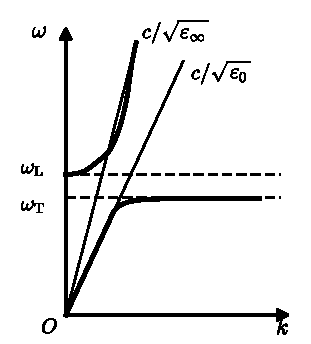
\includegraphics[width=7cm]{fig2-8.pdf}\\{\small 图 2.8\quad 极化激元的色散曲线}
\end{minipage}
\end{center}

\begin{center}
\begin{minipage}{6cm}
\centering
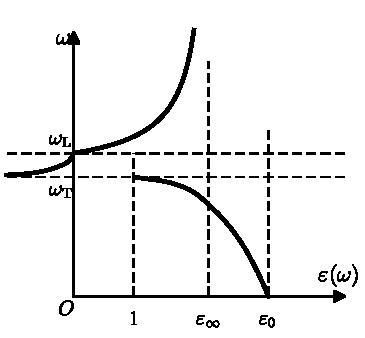
\includegraphics[width=6cm]{fig2-9.pdf}\\{\small 图 2.9\quad 极化激元的介电函数}
\end{minipage}
\end{center}

\begin{center}
\begin{minipage}{6cm}
\centering
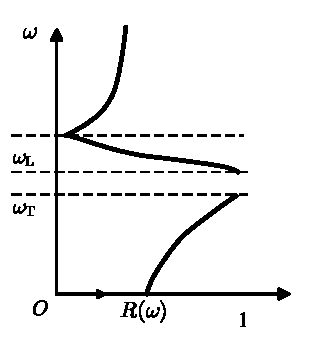
\includegraphics[width=6cm]{fig2-10.pdf}\\{\small 图 2.10\quad 反射比曲线}
\end{minipage}
\end{center}

利用式(2.7.4)与式(2.6.28)，可以导出极化激元的介电函数$\varepsilon(\omega)$与频率关系为
\begin{equation}
  \frac{k^2c^2}{\omega^2}=\varepsilon_{\infty}
  \frac{\omega_{\mathrm{L}}^2-\omega^2}{\omega_{\mathrm{T}}^2-\omega^2}
  =\varepsilon(\omega)
\end{equation}
图2.9是根据上式所作的$\varepsilon(\omega)$曲线.显然，在$\omega_{\mathrm{T}}<\omega<\omega_{\mathrm{L}}$频率范围内，介电函数取负值，它正好与耦合模的禁带相重合.当$\varepsilon(\omega)<0$时，由式(2.7.8)求得的$k$是纯虚数，代表指数衰减解，说明入射光不能在离子晶体中传播，与此同时实验上将观测到强烈的反射现象.例如，设晶体占据$z>0$半空间，对于沿正$z$方向垂直入射的电磁波，入射波的波数为$\frac{\omega}{c}$，而且入射的电场和磁场为
\begin{equation}
  E_x^{\mathrm{i}}=H_y^{\mathrm{i}}=A\mathrm{e}^{\mathrm{i}\omega\left(\frac{z}{c}-t\right)}
  \quad(z<0)
\end{equation}
由于在晶体界面上的反射波沿负$z$方向，其电场与磁场关系应设为
\begin{equation}
  E_x^{\mathrm{r}}=-H_y^{\mathrm{r}}\quad(z<0)
\end{equation}
为了决定$E_x^{\mathrm{r}}$及$H_y^{\mathrm{r}}$，我们还应当利用晶体中的极化激元解和$E_x$、$H_y$在真空与晶体界面两侧的连续条件.由式(2.7.2)和式(2.7.8)得到晶体中极化激元的电场为
\begin{equation}
  E_x=E_x(0)\mathrm{e}^{\mathrm{i}(kz-\omega t)}\quad(z>0)
\end{equation}
\begin{equation}
  k=\frac{\omega}{c}\sqrt{\varepsilon(\omega)}
\end{equation}
晶体中的$H_y$可从式(2.7.1)的第一个公式求得
\begin{equation}
  H_y=\sqrt{\varepsilon(\omega)}\,E_x\quad(z>0)
\end{equation}
再利用$z=0$界面两侧$E_x$与$H_y$的连续条件
\begin{equation}
\begin{gathered}
  E_x^{\mathrm{i}}+E_x^{\mathrm{r}}=E_x(0)\\[1ex]
  E_x^{\mathrm{i}}-E_x^{\mathrm{r}}=\sqrt{\varepsilon(\omega)}\,E_x(0)
\end{gathered}
\end{equation}
消去$E_x(0)$，求得入射波与反射波在界面上满足关系
\begin{equation}
  \frac{E_x^{\mathrm{i}}-E_x^{\mathrm{r}}}{E_x^{\mathrm{i}}+E_x^{\mathrm{r}}}
  =\sqrt{\varepsilon(\omega)}
\end{equation}
实验上测量的反射比定义为
\begin{equation}
  R(\omega)\equiv\biggl|\frac{E_x^{\mathrm{r}}}{E_x^{\mathrm{i}}}\biggr|^2
\end{equation}
它代表反射和入射电磁波在$z=0$处的强度比.由此立刻导出垂直入射时的反射比公式
\begin{equation}
  R(\omega)\equiv\biggl|
  \frac{\sqrt{\varepsilon(\omega)}-1}{\sqrt{\varepsilon(\omega)}+1}
  \biggr|^2
\end{equation}
从上式可知，当$\varepsilon(\omega)<0$时，$R(\omega)=1$，这时垂直入射的电磁波将在离子晶体表面被完全反射(图2.10)，与此同时在晶体中恰好没有极化激元的传播模式.以上讨论说明极化激元对于解释晶体中的光学现象起重要作用.

上述讨论表明：必须用TO声子与光子间耦合模(极化激元)的色散曲线才能全面解释电磁波在离子晶体中的传播特性.20世纪70年代以来，极化激元概念已推广到电磁波与固体中(包括表面、界面和超晶格)一切电性与磁性集体激发的线性耦合系统.人们将光子与TO声子、激子和磁振子等的耦合模量子都称作极化激元，并已为拉曼(Raman)光谱实验所证实.

\section{态密度}

当讨论晶体热力学性质时，往往涉及到对于各种独立格波的$(\boldsymbol{k},\sigma)$求和.由于波矢$\boldsymbol{k}$呈准连续分布，每一频带内的格波频率$\omega_{\sigma}(\boldsymbol{k})$也将是准连续分布的，因此在具体计算热力学量时，可以把$(\boldsymbol{k},\sigma)$的求和变换为对频率的积分，并同时引进态密度.平均每个元胞(或格点)的态密度$g(\omega)$定义为单位频率间隔内的格波模式数被总元胞数$N$除.对于三维复式晶体，当元胞内含有$s$个原子时，态密度的积分应等于平均每个元胞内的振动自由度$3s$.
\begin{equation}
  \int_0^{\infty}g(\omega)\mathrm{d}\omega=3s
\end{equation}
$g(\omega)$的具体表示式从晶格自由能引入.由于$(\boldsymbol{k},\sigma)$格波在简谐近似下的振动能量为
$\hbar\omega_{\sigma}(\boldsymbol{k})\left(n_{\boldsymbol{k}\sigma}+\frac{1}{2}\right)$，
其中$n_{\boldsymbol{k}\sigma}$为$(\boldsymbol{k},\sigma)$格波上激发的声子数.因此，声子数组态为$\{n_{\boldsymbol{k}\sigma}\}$时，系统的总振动能量为
\begin{equation*}
  E_{\{n_{\boldsymbol{k}\sigma}\}}
  =\sum_{\boldsymbol{k},\sigma}\hbar\omega_{\sigma}(\boldsymbol{k})
  \left(n_{\boldsymbol{k}\sigma}+\frac{1}{2}\right)
\end{equation*}
晶格振动的配分函数为
\begin{equation}
  Z=\sum_{\{n_{\boldsymbol{k}\sigma}\}}
  \exp(-\beta E_{\{n_{\boldsymbol{k}\sigma}\}})
  =\prod_{\boldsymbol{k},\sigma}
  \frac{\mathrm{e}^{-\frac{1}{2}\beta\hbar\omega_{\sigma}(\boldsymbol{k})}}
  {1-\mathrm{e}^{-\beta\hbar\omega_{\sigma}(\boldsymbol{k})}}
\end{equation}
其中$\beta=(1/k_{\mathrm{B}}T)$.按照热力学公式，不难从式(2.8.2)算得自由能
\begin{equation}
  F=-k_{\mathrm{B}}T\ln Z
  =k_{\mathrm{B}}T\sum_{\boldsymbol{k},\sigma}
  \ln\biggl[2\sinh\frac{\hbar\omega_{\sigma}(\boldsymbol{k})}{2k_{\mathrm{B}}T}\biggr]
\end{equation}
利用狄拉克$\delta$函数的特性
\begin{equation}
  f\bigl[\omega_{\sigma}(\boldsymbol{k})\bigr]
  \delta\bigl[\omega-\omega_{\sigma}(\boldsymbol{k})\bigr]
  =f(\omega)\delta\bigl[\omega-\omega_{\sigma}(\boldsymbol{k})\bigr]
\end{equation}
以及
\begin{equation}
  \int_0^{\infty}\delta\bigl[\omega-\omega_{\sigma}(\boldsymbol{k})\bigr]\mathrm{d}\omega=1
\end{equation}
可以将自由能公式(2.8.3)中的$\boldsymbol{k}$求和变换为对$\omega$的下列积分
\begin{equation}
\begin{aligned}
  F&=Nk_{\mathrm{B}}T\int_0^{\infty}
  \ln\Bigl[2\sinh\frac{\hbar\omega}{2k_{\mathrm{B}}T}\Bigr]
  \biggl\{\frac{1}{N}\sum_{\boldsymbol{k},\sigma}
  \delta\bigl[\omega-\omega_{\sigma}(\boldsymbol{k})\bigr]\biggr\}\mathrm{d}\omega\\
  &=Nk_{\mathrm{B}}T\int_0^{\infty}
  \ln\Bigl[2\sinh\frac{\hbar\omega}{2k_{\mathrm{B}}T}\Bigr]g(\omega)\mathrm{d}\omega
\end{aligned}
\end{equation}
其中
\begin{equation}
  g(\omega)\equiv\frac{1}{N}\sum_{\boldsymbol{k},\sigma}
  \delta\bigl[\omega-\omega_{\sigma}(\boldsymbol{k})\bigr]
\end{equation}
利用式(2.8.5)，容易证明所导出的态密度公式(2.8.7)满足关系式(2.8.1)，因为
\begin{equation*}
  \int_0^{\infty}g(\omega)\mathrm{d}\omega
  =\frac{1}{N}\sum_{\boldsymbol{k},\sigma}\int_0^{\infty}
  \delta\bigl[\omega-\omega_{\sigma}(\boldsymbol{k})\bigr]\mathrm{d}\omega
  =\frac{1}{N}\Bigl(\sum_{\boldsymbol{k},\sigma}1\Bigr)
  =\Bigl(\sum_{\sigma}1\Bigr)=3s
\end{equation*}
因此，式(2.8.7)给出晶格系统的正确态密度公式.

态密度$g(\omega)$是计算晶格热力学特性的重要物理量.利用式(2.8.6)可以求出晶格振动的内能$U$，热容$C_V$和熵$S$为
\begin{equation}
  U=F-T\Bigl(\frac{\partial F}{\partial T}\Bigr)_V
  =N\int_0^{\infty}\frac{1}{2}\hbar\omega
  \coth\Bigl(\frac{\hbar\omega}{2k_{\mathrm{B}}T}\Bigr)g(\omega)\mathrm{d}\omega
\end{equation}
\begin{equation}
  C_V=\Bigl(\frac{\partial U}{\partial T}\Bigr)_V
  =Nk_{\mathrm{B}}\int_0^{\infty}
  \left(\frac{\hbar\omega}{2k_{\mathrm{B}}T}\right)^2
  \mathrm{csch}^2\biggl(\frac{\hbar\omega}{2k_{\mathrm{B}}T}\biggr)
  g(\omega)\mathrm{d}\omega
\end{equation}
\begin{equation}
  S=-\Bigl(\frac{\partial F}{\partial T}\Bigr)_V
  =Nk_{\mathrm{B}}\int_0^{\infty}
  \biggl\{\frac{\hbar\omega}{2k_{\mathrm{B}}T}
  \coth\biggl(\frac{\hbar\omega}{2k_{\mathrm{B}}T}\biggr)
  -\ln\biggl[2\sinh\biggl(\frac{\hbar\omega}{2k_{\mathrm{B}}T}\biggr)\biggr]\biggr\}
  g(\omega)\mathrm{d}\omega
\end{equation}
显然，计算这些热力学量时都需要知道态密度的信息.

具体计算态密度时，常利用求和化积分公式(1.3.18)，将式(2.8.7)改写为下列形式
\begin{equation}
  g(\omega)=\frac{\Omega}{(2\pi)^3}\sum_{\sigma}
  \int_{\Omega^{*}}\delta\bigl[\omega-\omega_{\sigma}(\boldsymbol{k})\bigr]\mathrm{d}^3k
\end{equation}
其中$\Omega$为正点阵元胞体积，对$\boldsymbol{k}$的积分则限于一个倒点阵元胞$\Omega^{*}$.当格波的色散关系$\omega_{\sigma}(\boldsymbol{k})$为已知时，利用式(2.8.11)很容易计算态密度.例如，对于质量$M$，弹性力常数为$f$以及周期为$a$的一维原子链，固体物理学中已求得其格波频率为
\begin{equation}
  \omega^2(\boldsymbol{k})=\omega_{\mathrm{M}}^2
  \sin^2\Bigl(\frac{1}{2}ka\Bigr)
\end{equation}
其中$\omega_{\mathrm{M}}=2\sqrt{\frac{f}{M}}$是格波的最高频率.将式(2.8.12)代入式(2.8.11)，经简单运算得到晶格振动态密度为
\begin{equation}
\begin{aligned}
  g(\omega)&=\frac{a}{(2\pi)}\int_{-\pi/a}^{\pi/a}
  \delta\bigl[\omega-\omega(\boldsymbol{k})\bigr]\mathrm{d}k\\
  &=\frac{a}{\pi}\int_0^{\omega_{\mathrm{M}}}
  \left(\frac{\mathrm{d}k}{\mathrm{d}\omega}\right)
  \delta\bigl[\omega-\omega(\boldsymbol{k})\bigr]\mathrm{d}\omega(\boldsymbol{k})\\
  &=\frac{a}{\pi}\left(\frac{\mathrm{d}k}{\mathrm{d}\omega}\right)
  =\begin{cases}
  \dfrac{2}{\pi}\dfrac{1}{\sqrt{\omega_{\mathrm{M}}^2-\omega^2}}
  &(\omega<\omega_{\mathrm{M}})\\[3ex]
  0&(\omega>\omega_{\mathrm{M}})
  \end{cases}
\end{aligned}
\end{equation}
从上式可以看出，当$\omega=\omega_{\mathrm{M}}$时，
$|\nabla_{\boldsymbol{k}}\omega|=\frac{\mathrm{d}\omega}{\mathrm{d}k}=0$，
态密度$g(\omega_{\mathrm{M}})$发散.因此$|\nabla_{\boldsymbol{k}}\omega|=0$时，一维系统的态密度中将出现奇点.

为了更普遍讨论态密度在$|\nabla_{\boldsymbol{k}}\omega|=0$处的奇异特性，人们常将式(2.8.11)改写为沿等频面$S_{\omega}$的面积分公式，其作法如下：

首先将$\boldsymbol{k}$空间体元作变换
\begin{equation*}
  \mathrm{d}^3k\to\mathrm{d}S_{\omega}\,\mathrm{d}k_{\perp}
\end{equation*}
其中$\mathrm{d}S_{\omega}$是等频面上的面积元，而$\mathrm{d}k_{\perp}$是$\omega$与$\omega+\mathrm{d}\omega$等频面间垂直距离.由于$\mathrm{d}k_{\perp}$的方向与等频面元$\mathrm{d}S_{\omega}$的法线方向平行，因此
\begin{equation*}
  \mathrm{d}\omega=|\nabla_{\boldsymbol{k}}\omega|\,\mathrm{d}k_{\perp}
\end{equation*}
可求得
\begin{equation}
  \mathrm{d}k_{\perp}=\frac{\mathrm{d}\omega}{|\nabla_{\boldsymbol{k}}\omega|}
\end{equation}
把式(2.8.14)代入式(2.8.11)，可得到态密度的另一个表示式
\begin{equation}
  g(\omega)=\sum_{\sigma}\frac{\Omega}{(2\pi)^3}
  \int_{S_{\omega}}\frac{\mathrm{d}S_{\omega_{\sigma}}}
  {|\nabla_{\boldsymbol{k}}\omega_{\sigma}(\boldsymbol{k})|}
\end{equation}
由于在$|\nabla_{\boldsymbol{k}}\omega_{\sigma}(\boldsymbol{k})|=0$点上式中被积函数发散，因此这些点的态密度必然会表现出某种奇异性.人们将
$\nabla_{\boldsymbol{k}}\,\omega_{\sigma}(\boldsymbol{k})=0$的点称为范·霍夫(van\ Hove)奇点\textsuperscript{[2]}.

式(2.8.11)常用于计算各种近似模型的态密度，例如采用长波各向同性近似时，格波色散关系简化为
\begin{equation}
  \omega_{\sigma}(\boldsymbol{k})=c_{\sigma}k
\end{equation}
其中$\sigma$代表偏振指标，对于每个$\boldsymbol{k}$有一个纵波和两个横波，纵波和横波的声速分别为$c_{\mathrm{L}}$与$c_{\mathrm{T}}$.由于$\omega_{\sigma}(\boldsymbol{k})$与$\boldsymbol{k}$的方向无关，因此等频面是球面，我们可以将积分区域$\Omega^{*}$用等体积的球代替，即
\begin{equation*}
  \Omega^{*}=\frac{(2\pi)^3}{\Omega}
  =\frac{(2\pi)^3N}{V}=\frac{4\pi}{3}k_{\mathrm{D}}^3
\end{equation*}
其中等体积球的半径为$k_{\mathrm{D}}$，它等于
\begin{equation}
  k_{\mathrm{D}}=\left(6\pi^2\frac{N}{V}\right)^{1/3}
\end{equation}
它就是德拜(Debye)模型中的最大波数.这时式(2.8.11)可写成
\begin{equation}
\begin{aligned}
  g(\omega)&=\sum_{\sigma}\frac{\Omega}{(2\pi)^3}\int_0^{k_{\mathrm{D}}}
  \delta\bigl[\omega-\omega_{\sigma}(\boldsymbol{k})\bigr]4\pi k^2\mathrm{d}k\\
  &=\begin{cases}
  \dfrac{9\omega^2}{\omega_{\mathrm{D}}^3}&(\omega<\omega_{\mathrm{D}})\\[2ex]
  0&(\omega>\omega_{\mathrm{D}})
  \end{cases}
\end{aligned}
\end{equation}
这里的$\omega_{\mathrm{D}}$为德拜频率，满足关系式
\begin{equation}
  \omega_{\mathrm{D}}=ck_{\mathrm{D}}
\end{equation}
其中$c$代表
\begin{equation*}
  \frac{3}{c^3}=\frac{1}{c_{\mathrm{L}}^3}+\frac{2}{c_{\mathrm{T}}^3}
\end{equation*}
式(2.8.18)就是固体物理学中熟知的德拜态密度.

式(2.8.11)与式(2.8.15)是态密度的两个等效表示式，他们不仅适用于晶格振动，若将这两个公式中的格波频率换成能带电子的能量$E_n(\boldsymbol{k})$，则得到平均每个格点的电子态密度的相应表示式
\begin{equation}
\begin{aligned}
  g(\omega)&=\sum_{\sigma}\frac{\Omega}{(2\pi)^3}\int_{\Omega^{*}}
  \delta\bigl[E-E_n(\boldsymbol{k})\bigr]\mathrm{d}^3k\\
  &=2\,\frac{\Omega}{(2\pi)^3}\int_{\Omega^{*}}
  \delta\bigl[E-E_n(\boldsymbol{k})\bigr]\mathrm{d}^3k
\end{aligned}
\end{equation}
\begin{equation}
  g(\omega)=2\,\frac{\Omega}{(2\pi)^3}
  \int_{S_E}\frac{\mathrm{d}S_E}{|\nabla_{\boldsymbol{k}}E_n(\boldsymbol{k})|}
\end{equation}
这里$\sigma$代表电子自旋指标，由于$E_n(\boldsymbol{k})$与$\sigma$无关，因此对$\sigma$求和简化为乘自旋简并度2.对于自由电子模型
\begin{equation}
  E(\boldsymbol{k})=\frac{\hbar^2k^2}{2m}
\end{equation}
式(2.8.20)中体元$\mathrm{d}^3k$可变换为
$4\pi k^2\mathrm{d}k\sim\sqrt{E(\boldsymbol{k})}\,\mathrm{d}E(\boldsymbol{k})$，
于是求得$g(E)\sim\sqrt{E}$，此即自由电子气的态密度.

\section{范·霍夫奇点}

现在讨论$|\nabla_{\boldsymbol{k}}\,\omega(\boldsymbol{k})|$等于零时态密度的奇异性.为简单起见，只取态密度面积公式中某一支频带，并略去$\sigma$指标，则式(2.8.15)简化为
\begin{equation}
  g(\omega)=\frac{\Omega}{(2\pi)^3}
  \int_{S_{\omega}}\frac{\mathrm{d}S_{\omega}}
  {|\nabla_{\boldsymbol{k}}\omega(\boldsymbol{k})|}
\end{equation}
这个公式告诉我们当波包群速$\nabla_{\boldsymbol{k}}\omega$为零时，$g(\omega)$中将出现范·霍夫奇点.由于在三维晶格中$\nabla_{\boldsymbol{k}}\omega$在$\omega-k$色散曲线的极小点，极大点和鞍点处为零，因此在这些点附近可将$\omega$的展开式写成
\begin{equation}
  \omega(\boldsymbol{k})=\omega(\boldsymbol{k}_0)
  +\sum_{i=1}^{3}\alpha_i(\boldsymbol{k}-\boldsymbol{k}_0)_i^2
\end{equation}
其中$\alpha_i$是在主轴坐标系中的展开系数，而$\boldsymbol{k}_0$为范·霍夫奇点的波矢，它满足
\begin{equation}
  \bigl[\nabla_{\boldsymbol{k}}\,\omega(\boldsymbol{k})\bigr]_{\boldsymbol{k}=\boldsymbol{k}_0}=0
\end{equation}
由式(2.9.3)可知，共有4类范·霍夫奇点，它们分别对应于：

(i)$\alpha_1$，$\alpha_2$，$\alpha_3>0$：代表$\omega(\boldsymbol{k})$的极小点用$M_0$标记；

(ii)$\alpha_1$，$\alpha_2$，$\alpha_3<0$：代表$\omega(\boldsymbol{k})$的极大点用$M_3$标记；

(iii)$\alpha_1$，$\alpha_2>0$，$\alpha_3<0$：代表$\omega(\boldsymbol{k})$的Ⅰ类鞍点，用$M_1$标记；

(iv)$\alpha_1$，$\alpha_2<0$，$\alpha_3>0$：代表$\omega(\boldsymbol{k})$的Ⅱ类鞍点用$M_2$标记.

试问这些点在态密度曲线上如何表现？我们将按照瓦尼尔的说法\textsuperscript{[3]}，介绍范·霍夫奇点附近态密度的特性.首先作标度变换，令
\begin{equation}
  r_i=\sqrt{|\alpha_i|}\,(\boldsymbol{k}-\boldsymbol{k}_0)_i
\end{equation}
代入式(2.9.2)，求得在上述4类范·霍夫奇点附近$\omega(\boldsymbol{k})$的展开式为
\begin{equation}
  \omega(\boldsymbol{k})-\omega(\boldsymbol{k}_0)
  =\sum_{i=1}^{3}\varepsilon_ir_i^2\quad(\varepsilon_i=\pm1)
\end{equation}
再利用态密度的另一个等效表示式(2.8.11)，具体确定在$\omega(\boldsymbol{k}_0)$附近$g(\omega)$的行为.对于单频带情况，式(2.8.11)简化为
\begin{equation}
  g(\omega)=\frac{\Omega}{(2\pi)^3}\int_{\Omega^{*}}
  \mathrm{d}^3k\,\delta[\omega-\omega(\boldsymbol{k})]
\end{equation}
下面分别讨论4类范·霍夫奇点：

(i)$\varepsilon_1=\varepsilon_2=\varepsilon_3=1$情况

这时在频率轴上$\omega(\boldsymbol{k}_0)$为极小点$M_0$，在新坐标系$r_i$中等频面是球面.式(2.9.5)变为
\begin{equation}
  \omega(\boldsymbol{k})-\omega(\boldsymbol{k}_0)=r^2
  \quad\Bigl(r^2=\sum_{i=1}^{3}r_i^2\Bigr)
\end{equation}
利用式(2.9.4)—(2.9.7)算得
\begin{equation}
\begin{aligned}
  g(\omega)&=\frac{\Omega}{(2\pi)^3}
  \frac{4\pi}{\sqrt{|\alpha_1||\alpha_2||\alpha_3|}}
  \int r^2\mathrm{d}r\,\delta\bigl[\omega-\omega(\boldsymbol{k}_0)-r^2\bigr]\\
  &=\frac{\Omega}{(2\pi)^3}
  \frac{2\pi}{\sqrt{|\alpha_1||\alpha_2||\alpha_3|}}
  \,\bigl|\omega-\omega(\boldsymbol{k}_0)\bigr|^{\frac{1}{2}}\times\\
  &\quad\bigl\{1+\mathrm{sgn}\bigl[\omega-\omega(\boldsymbol{k}_0)\bigr]\bigr\}
\end{aligned}
\end{equation}
其中
\begin{equation}
  \mathrm{sgn}\,x=\begin{cases}
  1&(x>0)\\
  -1&(x<0)
  \end{cases}
\end{equation}
因此，在极小点$M_0$附近的态密度
\begin{equation}
  g(x)\sim\begin{cases}
  \bigl[\omega-\omega(\boldsymbol{k}_0)\bigr]^{1/2}
  &\bigl[\omega>\omega(\boldsymbol{k}_0)\bigr]\\
  0&\bigl[\omega<\omega(\boldsymbol{k}_0)\bigr]
  \end{cases}
\end{equation}
如图2.11(a)所示，$g(\omega)$以正无限大斜率离开极小点，这是三维情况下$M_0$型范·霍夫奇点的特征.

(ii)$\varepsilon_1=\varepsilon_2=\varepsilon_3=-1$情况

对应于极大点$M_3$，作类似情况(1)的计算，容易证明在$M_3$型奇点附近
\begin{equation}
\begin{aligned}
  g(\omega)&=\frac{\Omega}{(2\pi)^3}
  \frac{2\pi}{\sqrt{|\alpha_1||\alpha_2||\alpha_3|}}
  \,\bigl|\omega-\omega(\boldsymbol{k}_0)\bigr|^{\frac{1}{2}}\times\\
  &\quad\bigl\{1-\mathrm{sgn}\bigl[\omega-\omega(\boldsymbol{k}_0)\bigr]\bigr\}
\end{aligned}
\end{equation}
因此有
\begin{equation}
  g(\omega)\sim\bigl[\omega(\boldsymbol{k}_0)-\omega\bigr]^{1/2}
  \quad\bigl[\omega<\omega(\boldsymbol{k}_0)\bigr]
\end{equation}
说明在$g(\omega)$以负无限大斜率接近$M_3$型范·霍夫奇点，如图2.11(b)所示.

(iii)$\varepsilon_1=\varepsilon_2=1$，$\varepsilon_3=-1$情况

这时$\omega(\boldsymbol{k}_0)$为Ⅰ类鞍点$M_1$，式(2.9.5)可写成
\begin{equation}
  \omega(\boldsymbol{k})-\omega(\boldsymbol{k}_0)
  =\bigl(r_1^2+r_2^2\bigr)-r_3^2
\end{equation}
令
\begin{equation}
  \bigl|\omega(\boldsymbol{k})-\omega(\boldsymbol{k}_0)\bigr|=a^2
\end{equation}
当$\omega(\boldsymbol{k})>\omega(\boldsymbol{k}_0)$时式(2.9.13)变为
\begin{equation}
  r_1^2+r_2^2-r_3^2=a^2
\end{equation}
是单叶双曲面.当$\omega(\boldsymbol{k})<\omega(\boldsymbol{k}_0)$时，式(2.9.14)应写为
\begin{equation}
  r_1^2+r_2^2-r_3^2=-a^2
\end{equation}
代表双叶双曲面，而当$\omega(\boldsymbol{k})=\omega(\boldsymbol{k}_0)$时，有方程
\begin{equation}
  r_1^2+r_2^2=r_3^2
\end{equation}
则是过鞍点$M_1$的圆锥面.在$M_1$附近$g(\omega)$的行为应由上述等频面的变化决定，利用类似于椭球坐标变换的技巧，分别对$\omega(\boldsymbol{k})>\omega(\boldsymbol{k}_0)$和$\omega(\boldsymbol{k})<\omega(\boldsymbol{k}_0)$两种情况作下列变换\textsuperscript{[4]}：

(1)当$\omega(\boldsymbol{k})>\omega(\boldsymbol{k}_0)$时，令
\begin{equation}
\left.\begin{aligned}
  &r_1=a\cosh\xi\cos\phi\\
  &r_2=a\cosh\xi\sin\phi\\
  &r_3=a\sinh\xi
\end{aligned}\right\}
\end{equation}
其中$0\leqslant\phi\leqslant2\pi$，$0<\xi<\infty$.再利用雅可比(Jacobian)行列式求出变换前后的体元关系.
\begin{equation}
  \mathrm{d}r_1\mathrm{d}r_2\mathrm{d}r_3
  =\frac{1}{2}\bigl[\omega(\boldsymbol{k})-\omega(\boldsymbol{k}_0)\bigr]^{\frac{1}{2}}
  \mathrm{d}\omega(\boldsymbol{k})\,\mathrm{d}\sinh\xi\,\mathrm{d}\phi
\end{equation}
(2)当$\omega(\boldsymbol{k})<\omega(\boldsymbol{k}_0)$时，设
\begin{equation}
\left.\begin{aligned}
  &r_1=a\sinh\xi\cos\phi\\
  &r_2=a\sinh\xi\sin\phi\\
  &r_3=a\cosh\xi
\end{aligned}\right\}
\end{equation}
得到
\begin{equation}
  \mathrm{d}r_1\mathrm{d}r_2\mathrm{d}r_3
  =\frac{1}{2}\bigl[\omega(\boldsymbol{k}_0)-\omega(\boldsymbol{k})\bigr]^{\frac{1}{2}}
  \mathrm{d}\omega(\boldsymbol{k})\,\mathrm{d}\cosh\xi\,\mathrm{d}\phi
\end{equation}
态密度公式(2.9.6)经变换后写为
\begin{equation}
\begin{aligned}
  g(\omega)&=\frac{\Omega}{(2\pi)^3}
  \frac{1}{\sqrt{|\alpha_1||\alpha_2||\alpha_3|}}\times\\
  &\quad\int_{\sum_{i=1}^{3}r_i^2<R^2}
  \mathrm{d}r_1\mathrm{d}r_2\mathrm{d}r_3\,
  \delta\bigl[\omega-\omega(\boldsymbol{k})\bigr]
\end{aligned}
\end{equation}
其中$\sum_{i=1}^{3}r_i^2<R^2$的限制条件来源于式(2.9.6)要求积分限于$\Omega^{*}$之内，而$R$是某个固定的数.这一限制对$\xi$的积分限有较大影响，因为
\begin{equation}
  \sum_{i=1}^{3}r_i^2=a^2\cosh2\xi<R^2
\end{equation}
当$\omega=\omega(\boldsymbol{k})>\omega(\boldsymbol{k}_0)$时，由式(2.9.15)和式(2.9.24)得到
\begin{equation}
  \cosh2\xi<\frac{R^2}{[\omega-\omega(\boldsymbol{k}_0)]}
\end{equation}
因此$\sinh\xi$的积分限是
\begin{equation}
  0<\sinh\xi<\sqrt{\frac{1}{2}\biggl[\left(\frac{R}{a}\right)^2-1\biggr]}
\end{equation}
但$\phi$的积分限不变，仍为0到$2\pi$.这时由式(2.9.22)容易算出
$\omega>\omega(\boldsymbol{k}_0)$时$M_1$点附近的态密度为
\begin{equation}
  g(\omega)\sim\pi\sqrt{\frac{1}{2}\bigl[R^2+\omega(\boldsymbol{k}_0)-\omega\bigr]}
  \quad\bigl[\omega>\omega(\boldsymbol{k}_0)\bigr]
\end{equation}
它以连续有限的斜率离开$\omega(\boldsymbol{k}_0)$点.当$\omega=\omega(\boldsymbol{k})<\omega(\boldsymbol{k}_0)$时，按照式(2.9.14)取
$a^2=[\omega(\boldsymbol{k}_0)-\omega]$，限制条件变为
\begin{equation}
  \cosh2\xi<\frac{R^2}{[\omega(\boldsymbol{k}_0)-\omega]}
\end{equation}
相应的$\cosh\xi$的积分限是
\begin{equation}
  1<\cosh\xi<\sqrt{\frac{1}{2}\biggl[\left(\frac{R}{a}\right)^2+1\biggr]}
\end{equation}
算出的态密度为
\begin{equation}
  g(\omega)\sim\pi\biggl\{\sqrt{\frac{1}{2}\bigl[R^2+\omega(\boldsymbol{k}_0)-\omega\bigr]}
  -\sqrt{\omega(\boldsymbol{k}_0)-\omega}\biggr\}
  \quad\bigl[\omega<\omega(\boldsymbol{k}_0)\bigr]
\end{equation}
比较式(2.9.26)与式(2.9.29)可以看出，在$\omega(\boldsymbol{k}_0)$点$g(\omega)$仍是连续的，但是$g(\omega)$的斜率有不连续的变化，式(2.9.29)右边第二项的导数在$\omega(\boldsymbol{k}_0)$点趋于正无穷大，如图2.11(c)所示.由此可知，在$M_1$型鞍点附近态密度的导数表现出奇异性.

(iv)$\varepsilon_1=\varepsilon_2=-1$，$\varepsilon_3=1$情况

属于Ⅱ类鞍点$M_2$，其讨论与情况(3)类似，所得结果如图2.11(d)所示.显然，在$M_2$奇点附近$g'(\omega)$也有不连续变化，不同的只是$g(\omega)$以负无穷大斜率离开$\omega(\boldsymbol{k}_0)$点.

根据以上讨论可知，如果定出了范·霍夫奇点$\omega(\boldsymbol{k}_0)$的位置，就能作出这些点附近的态密度曲线.因此，利用范·霍夫奇异性可以简化态密度的计算，关于这方面工作的深入讨论见文献\textsuperscript{[5]}.

\begin{center}
\begin{minipage}{10.5cm}
\centering
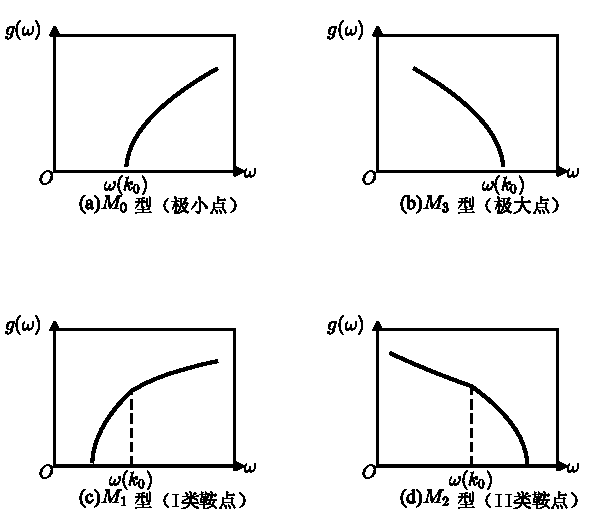
\includegraphics[width=10.5cm]{fig2-11.pdf}\\{\small 图 2.11\quad 范·霍夫奇点附近的态密度}
\end{minipage}
\end{center}

\section{晶格振动的局域模}

含有杂质和缺陷的晶体，由于平移对称性被破坏，其声子谱将不同于完整晶格，会产生以杂质、缺陷为中心的局域振动模式.

作为问题的第一步，我们将讨论单个杂质或缺陷对晶格振动谱的影响.从一维原子链入手，设质量为$M$的原子组成一维简单晶格，元胞数为$N$，在原点$(l=0)$处有一个质量为$M'$的杂质原子，近邻互作用的弹性力常数均设为$f$，如图2.12所示.因此
\begin{equation}
  M_1=\begin{cases}
  M&(l\neq0)\\
  M'&(l=0)
  \end{cases}
\end{equation}
并设
\begin{equation}
  \varepsilon\equiv\frac{M-M'}{M}
\end{equation}

\begin{center}
\begin{minipage}{9cm}
\centering
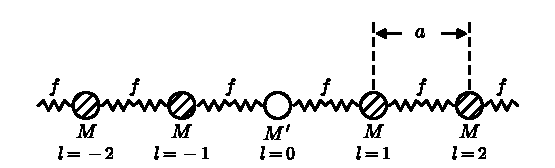
\includegraphics[width=9cm]{fig2-12.pdf}\\{\small 图 2.12\quad 含单个缺陷的一维链模型}
\end{minipage}
\end{center}

当$\varepsilon>0$时，代表“轻杂质”情况，而$\varepsilon<0$属于“重杂质”.由于杂质的存在，晶格振动的哈密顿量
\begin{equation}
  H=T+V
\end{equation}
其中动能部分
\begin{equation}
  T=\frac{1}{2}M\sum_l\dot{u}_l^2
  +\frac{1}{2}\bigl(M'-M\bigr)\dot{u}_{l=0}^2
\end{equation}
在简谐近似下根据图2.12规定的模型，其位能部分可简单写为
\begin{equation}
  V=\frac{1}{2}f\sum_l\bigl(u_l-u_{l+1}\bigr)^2
\end{equation}
$u_l$代表$l$元胞中原子的位移.下面将分别讨论式(2.10.3)的频谱及振动模特征.

\subsection*{1. 单个缺陷对振动频率的影响}

由于缺陷的存在，平移对称性被破坏，我们不能直接利用布洛赫定理来确定系统的振动模式，但可以利用傅里叶变换使求解简化，根据式(1.5.12)，晶格振动位移可表示为
\begin{equation}
  u_l=\frac{1}{\sqrt{N}}\sum_k\xi_k\mathrm{e}^{-\mathrm{i}kla}
\end{equation}
其中$k$限于BZ.将式(2.10.6)代入式(2.10.4)和式(2.10.5)，并利用关系式
\begin{equation}
  \frac{1}{N}\sum_l\mathrm{e}^{-\mathrm{i}(k+k')la}=\delta_{k',-k}
\end{equation}
可将$T$、$V$改用$\xi_k$、$\dot{\xi}_k$表示
\begin{equation}
\left.\begin{aligned}
  &T=\frac{1}{2}M\sum_k\dot{\xi}_k\dot{\xi}_{-k}
  +\frac{M'-M}{2N}\Bigl[\sum_k\dot{\xi}_k\Bigr]^2\\
  &V=\frac{1}{2}M\sum_k\omega_k^2\xi_k\xi_{-k}
\end{aligned}\right\}
\end{equation}
其中
\begin{equation}
  \omega_k^2=\omega_{\mathrm{M}}^2\sin^2\frac{ka}{2}
  \quad\left(\omega_{\mathrm{M}}^2=\frac{4f}{M}\right)
\end{equation}
代表完整晶格的本征振动频率，是$k$波矢格波的频率，属于平面波型解或称简正模.由于$M'$出现系统的本征频将发生改变，根据经典力学含缺陷系统的运动方程变为
\begin{equation}
  M\ddot{\xi}_k+\frac{M'-M}{N}\sum_k\ddot{\xi}_k
  =-M\omega_k^2\xi_k
\end{equation}
设$\xi_k\sim\exp(-\mathrm{i}\omega t)$，并利用式(2.10.2)将上式改写成
\begin{equation}
  \omega^2\Bigl(\xi_k-\frac{\varepsilon}{N}\sum_k\xi_k\Bigr)
  =\omega_k^2\xi_k
\end{equation}
考虑$\xi_k$的非零解，设
\begin{equation}
  \xi=\frac{1}{N}\sum_k\xi_k
\end{equation}
求得
\begin{equation}
  \xi_k=\varepsilon\,\frac{\xi\omega^2}{\bigl(\omega^2-\omega_k^2\bigr)}
\end{equation}
上式对$k$求和，再利用式(2.10.12)并消去$\xi$，得到确定含缺陷系统本征频率的方程为
\begin{equation}
  1=\frac{\varepsilon\omega^2}{N}\sum_k
  \frac{1}{\omega^2-\omega_k^2}\equiv F\bigl(\omega^2\bigr)
\end{equation}
式(2.10.14)可用作图法求解.图2.13(a)、(b)分别表示
$\varepsilon<0\,(M'>M$，重杂质$)$和$\varepsilon>0\,(M'<M$，轻杂质$)$情况.完整晶格的简正模频率$\omega_k$限于$0\to\omega_{\mathrm{M}}$区间，由图中黑点“$\bullet$”表示，图中“$\blacktriangle$”号代表含缺陷晶格的本征频率，它们满足式(2.10.14).显然，$F$函数是$\omega$的偶函数，在这里只画出了$\omega>0$部分，因为简单晶格的声频支解的最低频率为$\omega=0$.

由图2.13(a)可知，对于“重杂质”情况$(\varepsilon<0)$，式(2.10.14)的解仍落于声频支许可频带之内，非完整晶格的解(“$\blacktriangle$”)与完整晶格的简正模解(“$\bullet$”)有一一对应关系.由于杂质原子质量$M'$大于基体原子质量$M$，所有的解都向低频方向略有移动，其移动大小不超过两个近邻$\omega_k$值之差.又因为声频支频带下限在$\omega=0$处，这里没有单独的模式被推出频带底部.图中$\omega=0$模式解不明显出现，只是由于作图时所选用函数$F(\omega^2)$在$\omega=0$处无定义的缘故.

在图2.13(b)中$0<\varepsilon<1$，属于“轻杂质”情况.当$\omega<\omega_{\mathrm{M}}$时，式(2.10.14)的解相对于$\omega_k$都朝高频方向略有移动，在这里非完整晶格的解比$\omega_k$解少一个.这个解的移动较大，它被推出准连续频带顶部$(\omega_{\mathrm{M}})$，落在$\omega>\omega_{\mathrm{M}}$区域中，形成一个孤立的能级.通过下面的分析将明白，$\varepsilon>0$情况下$\omega>\omega_{\mathrm{M}}$的孤立解代表以杂质原子为中心的局域振动模式.

\begin{center}
\begin{minipage}{9.5cm}
\centering
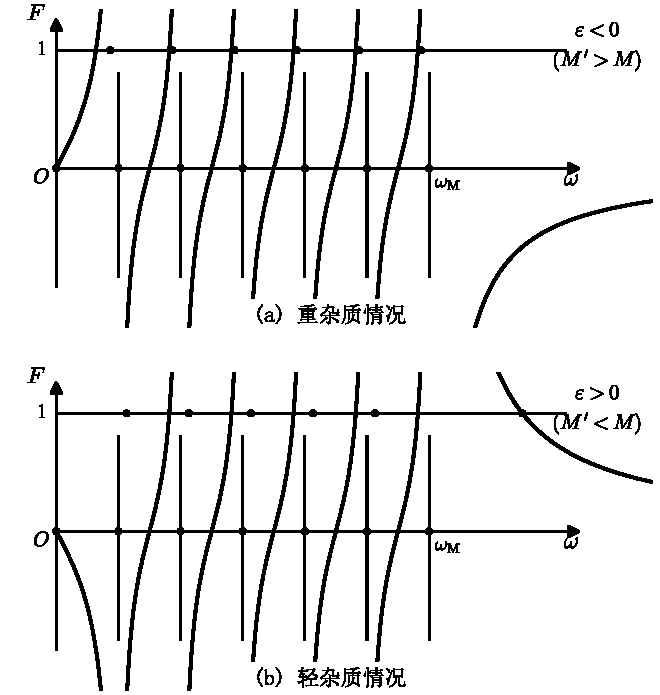
\includegraphics[width=9.5cm]{fig2-13.pdf}\\{\small 图 2.13\quad 式(2.10.14)的作图解}
\end{minipage}
\end{center}

\subsection*{2. 局域模\textsuperscript{[6]}}

为了分析振动模式，必须解$u_l$的运动方程.根据式(2.10.4)、(2.10.5)和(2.10.2)容易写出运动方程
\begin{equation}
  M\ddot{u}_l-f\bigl(u_{l+1}+u_{l-1}-2u_l\bigr)
  =\varepsilon M\ddot{u}_0\delta_{l0}
\end{equation}
其中$\delta_{l0}$为克罗尼克(Kr\"onecker)$\delta$函数.令$u_l\sim\exp(-\mathrm{i}\omega t)$.将上式写为
\begin{equation}
  u_1+u_{-1}
  +\biggl[\frac{4\omega^2}{\omega_{\mathrm{M}}^2}(1-\varepsilon)-2\biggr]u_0=0
\end{equation}
和
\begin{equation}
  u_{l+1}+u_{l-1}
  +\left(\frac{4\omega^2}{\omega_{\mathrm{M}}^2}-2\right)u_l=0
  \quad(l\neq0)
\end{equation}
其中$\omega_{\mathrm{M}}^2=\frac{4f}{M}$.振动的特征应由式(2.10.16)与(2.10.17)的联立解确定.由于杂质位于$l=0$点，这里存在着对称解$(u_l=u_{-l})$和反对称解$(u_l=-u_{-l})$.反对称解要求$u_0=0$和$u_l+u_{-l}=0$，因此式(2.10.16)不起作用，可不讨论.下面仅研究对称解，可设解的一般形式为
\begin{equation}
  u_l=A\lambda^{|l|}+B\lambda^{-|l|}
\end{equation}
代入式(2.10.17)得到
\begin{equation}
  \lambda^2+1+\left(\frac{4\omega^2}{\omega_{\mathrm{M}}^2}-2\right)\lambda=0
\end{equation}
由式(2.10.19)可以判断$\lambda$根的性质.当$\omega<\omega_{\mathrm{M}}$时，方程有复根，可设$\lambda$为$\exp(\mathrm{i}\theta)$形式并取$\theta=ka$，属于格波解.当$\omega>\omega_{\mathrm{M}}$时$\lambda$有负实根，其中一个$|\lambda|<1$、另一个$|\lambda|>1$，这时将求得局域晶格振动解.下面分别讨论：

(i)对于$\omega<\omega_{\mathrm{M}}$情况：可令
\begin{equation}
  u_l=A\exp(\mathrm{i}ka|l|)+B\exp(-\mathrm{i}ka|l|)
\end{equation}
代入式(2.10.16)得到方程
\begin{equation}
  \frac{A\exp(\mathrm{i}ka)+B\exp(-\mathrm{i}ka)}{A+B}
  +\biggl[\frac{2\omega^2}{\omega_{\mathrm{M}}^2}(1-\varepsilon)-1\biggr]=0
\end{equation}
考虑到$u_l$为实量，应有$A^{*}=B$关系.因此，可进一步假定
\begin{equation}
  A=\frac{c}{2}\exp(-\mathrm{i}\delta)\,,\quad
  B=\frac{c}{2}\exp(\mathrm{i}\delta)
\end{equation}
代入式(2.10.20)和式(2.10.21)求得在$0<\omega<\omega_{\mathrm{M}}$频带内的解
\begin{equation}
  u_l=c\cos\bigl(|l|ka-\delta\bigr)
\end{equation}
其中$\delta$代表相移，它满足方程
\begin{equation}
  \tan\delta=\varepsilon\tan\frac{ka}{2}
\end{equation}
以上结果说明，杂质的存在仅使简正模产生相移，相移的正负取决于$\varepsilon$的符号，这是和图2.13(a)及(b)中，$\omega<\omega_{\mathrm{M}}$时本征频率的微小移动相对应的.

(ii)对于$\omega>\omega_{\mathrm{M}}$的情况：讨论$|\lambda|<1$情况的负实根，这时可设对称解为
\begin{equation}
  u_l=A\lambda^{|l|}
\end{equation}
代入式(2.10.16)和式(2.10.17)得到方程组
\begin{equation}
\begin{gathered}
  2\lambda+\biggl[\frac{4\omega^2}{\omega_{\mathrm{M}}^2}(1-\varepsilon)-2\biggr]=0\\[1ex]
  \lambda^2+1+\left(\frac{4\omega^2}{\omega_{\mathrm{M}}^2}-2\right)\lambda=0
\end{gathered}
\end{equation}
联立求解可得
\begin{equation}
  (\lambda-1)\biggl[2-\frac{\lambda-1}{\lambda}(1-\varepsilon)\biggr]=0
\end{equation}
由于$\lambda\neq1$，因此$|\lambda|<1$的负根为
\begin{equation}
  \lambda=\frac{\varepsilon-1}{\varepsilon+1}
\end{equation}
其中$\varepsilon>0$，属于“轻杂质”情况.

将此解代入式(2.10.25)和式(2.10.26)第二个方程，给出位移
\begin{equation}
  u_l=u_0(-1)^l
  \left(\frac{1-\varepsilon}{1+\varepsilon}\right)^{|l|}
  \quad(\varepsilon>0)
\end{equation}
其振动频率
\begin{equation}
  \omega^2=\frac{\omega_{\mathrm{M}}^2}{1-\varepsilon}
\end{equation}
式(2.10.29)是以杂质为中心的衰减振荡解，其中近邻原子振动的方向相反，这就是晶格振动的局域模，其振动频率在$\omega_{\mathrm{M}}$之上，即图2.13(b)中的孤立能级，说明“轻杂质”将在声频支许可频带之上产生局域模.

局域模相当于$\lambda$取复数波矢$k$的解.若令
\begin{equation}
\left.\begin{aligned}
  &ka=\theta=\pi+\mathrm{i}Z\\
  &Z=\ln\left(\frac{1-\varepsilon}{1+\varepsilon}\right)
\end{aligned}\right\}
\end{equation}
则得到式(2.10.28)的结果
\begin{equation}
  \lambda=\mathrm{e}^{-\mathrm{i}ka}=\frac{\varepsilon-1}{\varepsilon+1}
\end{equation}
因此局域模又可写成下列指数形式
\begin{equation}
  u_l=u_0\mathrm{e}^{\mathrm{i}ka|l|}
\end{equation}
其中
\begin{equation}
  k=\frac{\pi}{a}+\mathrm{i}\frac{Z}{a}
\end{equation}
在一维链中的单个点缺陷(空位)与单杂质情况相似，这时$M'=0$，点缺陷的近邻常数应设为$f'$(与$f$不同).增大或减小单个力常数分别与减少或增大单个杂质原子的质量有相同的效应，读者可仿效以上做法自行处理点缺陷的局域模问题.

最后指出本节主要结论是：

(i)“轻杂质”将使简正模频率向上推移，并在许可频带之上分裂出一个局域模.增大杂质与基体原子的质量差$(\varepsilon)$，局域频率与许可频带上边界的距离也就拉得越开[见式(2.10.30)].

(ii)“重杂质”的效应是使本征频率向下移动，对于声频支振动许可频带的下界在$\omega=0$处，因此不可能在下界之外分裂出局域模.但是对于光频支振动，其许可频带的下界为非零值，在这种情况下“重杂质”就可能在频带之下产生一个分立能级——局域模.

\begin{canKao}
\begin{enumerate}[label={[\arabic*]}, leftmargin=2.2em, itemsep=0pt]
\item Born M, Huang K. Dynamical Theory of Crystal Lattice. Oxford: Clarenden Press, 1954
\item van Hove L. Phys Rev, 1953, 89: 1189
\item Wannier G H. Elements of Solid State Theory. London: Cambridge Univ Press, 1959
\item Callaway J. Quantum Theory of Solid State. New York: Academic Press, 1976
\item Maradudin A A. Solid State Phys. Suppl. 3 (2nd ed). New York: Academic Press, 1971
\item Madelung O. Introduction to Solid State Theory. New York: Springer Press, 1980. Chap9
\end{enumerate}
\end{canKao}

% ============================================================
%  第三章 磁振子（自旋波量子）（§1–§7 + 参考文献）
%  底本：高教社《固体理论》（第二版）印刷页 62–89（PDF p082–p109）
%  OCR 输入：full_merged.md 行 3227–4428
%
%  公式编号自检（smoke 单章编号首位为 1，全书装配后为 3）：
%    §2 (3.2.1)–(3.2.18) 18 式；§3 (3.3.1)–(3.3.42) 42 式；
%    §4 (3.4.1)–(3.4.18) 18 式；§5 (3.5.1)–(3.5.37) 37 式；
%    §6 (3.6.1)–(3.6.16) 16 式；§7 (3.7.1)–(3.7.20) 20 式；合计 151 式
%
%  已修正的 OCR 错误（择要，均经 150/300dpi 页面核实）：
%    1. 编号被 OCR 截断的 (3.2.17)、(3.3.27)、(3.7.3)、(3.7.11) 按原书补回，
%       均为实存编号、非跳号；(3.5.18) 为 OCR 漏检编号（p099/印刷79 实存，
%       即逆变换代入式(3.5.11)所得 H 的编号）。
%    2. §6 原书 (3.6.3a)(3.6.3b)、(3.6.7a)(3.6.7b)、(3.6.10a)(3.6.10b) 为带
%       字母的成对编号；重排本自动编号只能给单号，两式各合排于一个编号公式，
%       得 (3.6.3)(3.6.7)(3.6.10)，正文引用"式(3.6.3a)"等随之改为"式(3.6.3)"。
%    3. (3.7.1) 原书括号内两项均印作 Ŝ_l^+Ŝ_{l+δ}^-，第二项按其共轭项修正为
%       Ŝ_l^-Ŝ_{l+δ}^+（原书排印错误）。
%    4. (3.7.11) 原书首项印作 ∂α(x,t)/∂x，按薛定谔型方程修正为 ∂/∂t
%       （原书排印错误，由变换 α=e^{-iλt}φ(ξ,t) 可证）。
%    5. (3.2.4)–(3.2.6) 电子自旋算符 OCR 误作 a/σ/Γ，按 p084 统一为花体
%       \mathcal{s}（总自旋算符为 \boldsymbol{S}）；§5.3、§6 子格总自旋算符
%       按 p101/p105 为花体 \mathcal{S}（Δ\mathcal{S}_a^z）。
%    6. 被 OCR 打散的 (3.2.11)–(3.2.16) 矩阵、(3.6.8) 矩阵、(3.7.3) 四次项
%       算符串、(3.7.8) 末行等按 300dpi 页面重建。
%    7. (3.3.11) 条件按原书为 (n ≤ 2S)（OCR 误作 n ≪ 2S）；
%       (3.3.10) 括注（m=0,±1,⋯,±S）重建；§1 "但播"→"传播"、
%       "θxy 平面"→"Oxy 平面"；(3.4.4) 第 4 行按 p094 修复。
%   10. 原书排印疑误照录未改：§4 "按指数衰数"（疑为"衰减"）；
%       (3.3.39) 恒等式右端 γ_k∑γ_{k'}⟨n̂_{k'}⟩_T 照录；(3.4.17) 第二行指数
%       e^{+i(k·l−ω_k t)} 照录（与第一行不共轭，原书如此）；(3.7.14)
%       Q≡2(J'−J)/ħ 照录（由(3.7.11)推应为 4，原书如此）；文献[4] "John
%       Wiley & Sond"、文献[14] "Spinger-Verlag"、§7 "低维系" 照录。
% ============================================================
\chapter{磁振子（自旋波量子）}

\section{自旋波图像}

本章讨论自旋晶格系统的元激发.在固体物理学中已经阐明，由于交换作用，这个系统的基态是磁性离子自旋排列的有序状态.最常见的简单磁有序状态有：铁磁序、反铁磁序和铁淦氧磁序，它们分别如图3.1(a)、(b)、(c)所示.铁磁序为各格点上自旋取向一致的状态.反铁磁序和铁淦氧磁序描述相邻磁离子自旋取向相反的情况，它们仅在子晶格中具有自旋取向一致的特性.这是自旋-自旋互作用系统基态的图像.试问系统受微扰后的低能量激发态将以何种形式出现？现以铁磁体为例作如下定性说明：

\begin{center}
\begin{minipage}{6.5cm}
\centering
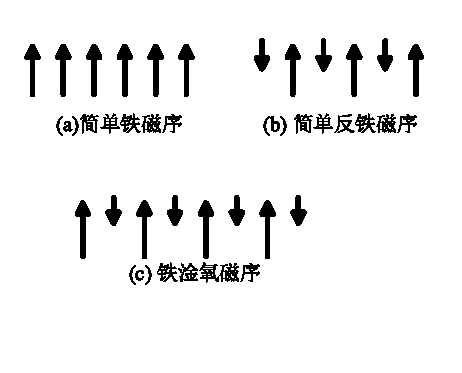
\includegraphics[width=6.5cm]{fig3-1.pdf}\\{\small 图 3.1\quad 自旋-自旋互作用系统的基态}
\end{minipage}
\end{center}

设铁磁体中某一个格点上的自旋 $\hat{\boldsymbol{S}}_l$ 因扰动偏离量子化轴方向，这时自旋间的交换作用使激发表现出如下特征：(i)$\hat{\boldsymbol{S}}_l$ 将带动近邻格点上自旋，而这些自旋又将使它们的近邻自旋取向改变，于是扰动以自旋集体运动的形式传播；(ii)近邻自旋对 $\hat{\boldsymbol{S}}_l$ 的作用要使它恢复原来取向以保持有序状态.这时在晶格中将形成离子自旋相对取向的振荡，图3.2是其经典图像.显然，由于各格点上进动自旋的方位角不同，磁激发具有类似波动的特性，这个波称为自旋波.

已经知道，通过弹性力耦合的晶格离子系统其低激发态是格波，而格波的量子称为声子.相似的，通过交换作用耦合的晶格自旋系统的低激发态以自旋波形式出现，自旋波的量子则称为磁振子.如果说声子是描述晶格离子间相对位移振荡的量子，那么磁振子就代表晶格自旋相对取向振荡的量子，它们都是互作用系统的集体激发.我们的任务是求铁磁体和反铁磁体中自旋波的频谱，涉及解自旋相互作用系统的本征态问题.为此，必须先考察自旋间相互作用的性质和哈密顿量的形式.

\begin{center}
\begin{minipage}{11cm}
\centering
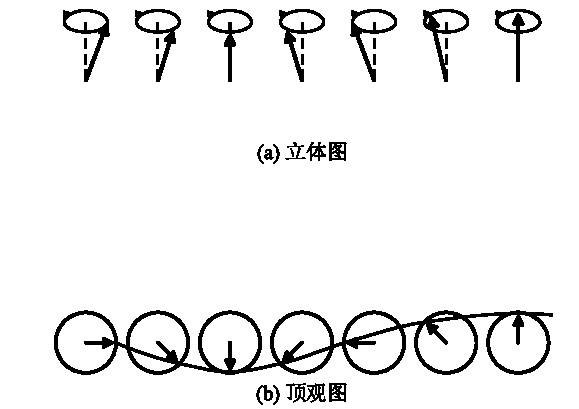
\includegraphics[width=11cm]{fig3-2.pdf}\\{\small 图 3.2\quad 自旋波的经典图像}
\end{minipage}
\end{center}

\section{海森伯模型及其严格推导}

\subsection*{1. 海森伯模型}

自旋-自旋相互作用系统的哈密顿量通常表示为
\begin{equation}
  H=-\sum_{l,l'}^{\prime}J_{ll'}\hat{\boldsymbol{S}}_l\cdot\hat{\boldsymbol{S}}_{l'}
\end{equation}
其中 $\hat{\boldsymbol{S}}_l$ 代表第 $l$ 个格点上磁性离子的矢量自旋算符，$\sum_{l,l'}^{\prime}$ 代表求和时不计 $l=l'$ 项，$J_{ll'}$ 是 $l$ 与 $l'$ 二格点离子上电子间的交换积分.
\begin{equation}
  J_{ll'}=J\left(\left|\boldsymbol{l}-\boldsymbol{l}'\right|\right)
\end{equation}
这里为简化记号令 $\boldsymbol{l}=\boldsymbol{R}_l$.式(3.2.1)与(3.2.2)就是海森伯模型\textsuperscript{[1]}，它是建立在如下一套假定之上的：

设两格点离子上各有一个自旋未配对的 d 电子，则根据量子力学，d 电子间交换能
\begin{equation}
  E_{\mathrm{ex}}=\pm J_{12}=\pm\int\phi_1^{*}\left(\boldsymbol{r}_1\right)\phi_2^{*}\left(\boldsymbol{r}_2\right)
  V\left(\boldsymbol{r}_{12}\right)\phi_1\left(\boldsymbol{r}_2\right)\phi_2\left(\boldsymbol{r}_1\right)
  \mathrm{d}\boldsymbol{r}_1\mathrm{d}\boldsymbol{r}_2
\end{equation}
其中 $V\left(\boldsymbol{r}\right)$ 为二格点系统的库仑互作用势，式(3.2.3)中正号对应于两个 d 电子自旋取向相反（$\uparrow\downarrow$）的状态，而负号代表两个 d 电子自旋取向一致（$\uparrow\uparrow$）.上式也可以等效地写为
\begin{equation*}
  E_{\mathrm{ex}}=\left\{\begin{array}{ll}
    +J_{12} & \mathcal{s}=0\\
    \left(\ \uparrow\downarrow\ ,\ \text{单重态}\right) & \\
    -J_{12} & \mathcal{s}=1\\
    \left(\ \uparrow\uparrow\ ,\ \text{三重态}\right) &
  \end{array}\right.
\end{equation*}
这里 $\mathcal{s}$ 为两格点间的组合自旋量子数，它是系统满足全同粒子不可区别性原理的直接结果.如用电子自旋算符描述，可求得两个电子系统的交换作用.由于
\begin{equation*}
  -\frac{1}{2}\left(1+4\hat{\mathcal{s}}_1\cdot\hat{\mathcal{s}}_2\right)
  =-\frac{1}{2}-\left(\hat{\boldsymbol{S}}^2-\hat{\mathcal{s}}_1^2-\hat{\mathcal{s}}_2^2\right)=\pm 1
\end{equation*}
其中 $+1$ 和 $-1$ 分别对应于总自旋算符 $\hat{\boldsymbol{S}}=\hat{\mathcal{s}}_1+\hat{\mathcal{s}}_2$ 的本征值取 $\mathcal{s}=0$ 或 $\mathcal{s}=1$，且有算符恒等式
\begin{equation*}
  \hat{\boldsymbol{S}}^2=\mathcal{s}\left(\mathcal{s}+1\right),\qquad
  \hat{\mathcal{s}}_1^2=\hat{\mathcal{s}}_2^2=\frac{1}{2}\left(\frac{1}{2}+1\right)=\frac{3}{4}
\end{equation*}
因此式(3.2.3)所对应的算符表示为
\begin{equation}
  H_{\mathrm{ex}}=-\frac{1}{2}J_{12}\left(1+4\hat{\mathcal{s}}_1\cdot\hat{\mathcal{s}}_2\right)
\end{equation}
略去常数项 $-\frac{1}{2}J_{12}$，求得两格点离子间的交换作用哈密顿量
\begin{equation}
  H_{12}=-2J_{12}\hat{\mathcal{s}}_1\cdot\hat{\mathcal{s}}_2
\end{equation}
尽管这里 $H_{12}$ 已表示成电子自旋矩间直接互作用的形式，但它来源于库仑势的交换作用项，互作用实为静电性的，不能理解为电子磁矩之间的直接磁作用.

将上式推广，应用到自旋大于 1/2 情况.这时每个离子上的自旋未配对 d 电子数大于 1，两格点间交换作用近似为
\begin{equation}
  H_{12}=-2J_{12}\sum_{i,j}\hat{\mathcal{s}}_{1i}\cdot\hat{\mathcal{s}}_{2j}
  =-2J_{12}\sum_i\hat{\mathcal{s}}_{1i}\cdot\sum_j\hat{\mathcal{s}}_{2j}
  =-2J_{12}\hat{\boldsymbol{S}}_1\cdot\hat{\boldsymbol{S}}_2
\end{equation}
其中 $\hat{\boldsymbol{S}}_1=\sum_i\hat{\mathcal{s}}_{1i}$，$\hat{\boldsymbol{S}}_2=\sum_j\hat{\mathcal{s}}_{2j}$ 分别为两格点上离子的总自旋算符.这里还作了两个假定：(i)同一格点的离子上的电子间交换作用可以忽略不计，(ii)两格点间所有电子具有相同的交换积分.

再进一步，计入所有格点间的交换作用推广到整个固体，就得到海森伯哈密顿量式(3.2.1).注意，当式(3.2.6)对 $l$、$l'$ 格点求和时应乘 1/2 因子以免计算重复.

在应用海森伯模型时，常采用更为简化的哈密顿量.考虑到交换积分的大小与格点间电子云的重叠程度有关，交换作用是短程作用，可以只计算近邻格点间的作用.若再假定 $J_{l,l+\delta}$ 为各向同性的常数 $J$，则海森伯模型表示为
\begin{equation}
  H=-J\sum_{l,\delta}\hat{\boldsymbol{S}}_l\cdot\hat{\boldsymbol{S}}_{l+\delta}
\end{equation}
$\delta$ 代表近邻格点间位置矢差.当 $J>0$ 时，式(3.2.7)的基态为铁磁序，当 $J<0$ 时可用于描述反铁磁性，当 $J<0$、并且近邻格点为不同磁离子（$S$ 不同）时，则描述亚铁磁性，即铁淦氧磁序.

\subsection*{2. 海森伯哈密顿量的推导}

在(1)中只介绍了海森伯引入交换作用的思路，而不是理论推导.狄拉克\textsuperscript{[2]}首先从多电子相互作用的哈密顿量出发导出了海森伯模型，其理论适用于磁性绝缘体，即晶体的电子处于局域化状态时式(3.2.1)可严格导出，下面仅介绍 $S=\frac{1}{2}$ 情况的推导.

设晶体中有 $N$ 个格点，每个格点上的离子只有一个未配对的局域态 d 电子.当研究 $N$ 个局域电子系统的交换作用时，我们应当采用瓦尼尔函数\footnote{关于瓦尼尔函数的详细讨论见第八章§8.}$a\left(\boldsymbol{r}-\boldsymbol{l}\right)$ 作基函数表示态矢量
$\Psi\left(\boldsymbol{r}\right)=\sum_{l,\sigma}C_{l\sigma}a\left(\boldsymbol{r}-\boldsymbol{l}\right)$.根据二次量子化的标准手续，用 $\Psi$ 对电子间库仑势 $\frac{e^2}{\left|\boldsymbol{r}-\boldsymbol{r}'\right|}$ 求平均，不难得到交换作用为
\begin{equation}
  H_{\mathrm{ex}}=-\frac{1}{2}\sum_{l,l'}^{\prime}\sum_{\sigma,\sigma'}J_{ll'}
  C_{l\sigma}^{+}C_{l\sigma'}C_{l'\sigma'}^{+}C_{l'\sigma}
\end{equation}
其中二体库仑积分
\begin{equation}
  J_{ll'}=e^2\int\frac{a^{*}\left(\boldsymbol{r}-\boldsymbol{l}\right)\,a\left(\boldsymbol{r}-\boldsymbol{l}'\right)\,
  a^{*}\left(\boldsymbol{r}'-\boldsymbol{l}'\right)\,a\left(\boldsymbol{r}'-\boldsymbol{l}\right)}
  {\left|\boldsymbol{r}-\boldsymbol{r}'\right|}\,\mathrm{d}^3r\,\mathrm{d}^3r'
\end{equation}
假如系统是绝缘体，则格点间无电子转移，即使跳跃电导也认为其概率很小可以忽略，这时每格点上只可能有一个未配对的 d 电子，它的自旋取向为朝上或朝下，但不存在空态和电子对态.换句话说，对于绝缘体应有 d 电子的单占据条件，它在数学上表示为下列算符形式，即
\begin{equation}
  C_{l\uparrow}^{+}C_{l\uparrow}+C_{l\downarrow}^{+}C_{l\downarrow}=1
\end{equation}
由式(3.2.10)不难求得泡利自旋算符
\begin{equation}
  \hat{\sigma}^{z}=\begin{pmatrix}1&0\\0&-1\end{pmatrix},\quad
  \hat{\sigma}^{+}=\begin{pmatrix}0&2\\0&0\end{pmatrix},\quad
  \hat{\sigma}^{-}=\begin{pmatrix}0&0\\2&0\end{pmatrix}
\end{equation}
和电子的产生及消灭算符之间有重要关系：
\begin{equation}
  \left.\begin{aligned}
    \hat{\sigma}^{z}&=C_{l\uparrow}^{+}C_{l\uparrow}-C_{l\downarrow}^{+}C_{l\downarrow}\\
    \hat{\sigma}_l^{+}&=2C_{l\uparrow}^{+}C_{l\downarrow}\\
    \hat{\sigma}_l^{-}&=2C_{l\downarrow}^{+}C_{l\uparrow}
  \end{aligned}\right\}
\end{equation}
其证明如下：

可以令
\begin{equation}
  C_{\uparrow}^{+}C_{\uparrow}\equiv\begin{pmatrix}1&0\\0&0\end{pmatrix}
\end{equation}
此矩阵作用于自旋朝上的单占据态 $\begin{pmatrix}1\\0\end{pmatrix}$ 得本征值 1，而作用于自旋朝下的单占据态
$\begin{pmatrix}0\\1\end{pmatrix}$ 其本征值为 0.这说明 $\begin{pmatrix}1&0\\0&0\end{pmatrix}$ 代表自旋朝上的占据数算符，与
$C_{\uparrow}^{+}C_{\uparrow}$ 的作用相同.因此，式(3.2.13)合理.将式(3.2.13)代入式(3.2.10)，又得到
\begin{equation}
  C_{\downarrow}^{+}C_{\downarrow}=\begin{pmatrix}0&0\\0&1\end{pmatrix}
\end{equation}
由于算符 $C_{\uparrow}^{+}C_{\downarrow}$ 使格点自旋从朝下态变为朝上态，故其作用应与
$\begin{pmatrix}0&1\\0&0\end{pmatrix}$ 相同.类似的，算符 $C_{\downarrow}^{+}C_{\uparrow}$ 应与
$\begin{pmatrix}0&0\\1&0\end{pmatrix}$ 作用相同.因此，还有下列对应关系：
\begin{equation}
  C_{\uparrow}^{+}C_{\downarrow}=\begin{pmatrix}0&1\\0&0\end{pmatrix},\quad
  C_{\downarrow}^{+}C_{\uparrow}=\begin{pmatrix}0&0\\1&0\end{pmatrix}
\end{equation}
利用式(3.2.13)—(3.2.15)，即可求出关系式(3.2.12)，或者换一个书写形式
\begin{equation}
  \left.\begin{aligned}
    C_{l\uparrow}^{+}C_{l\uparrow}&=\frac{1}{2}\left(1+\hat{\sigma}_l^{z}\right),&
    C_{l\downarrow}^{+}C_{l\downarrow}&=\frac{1}{2}\left(1-\hat{\sigma}_l^{z}\right)\\
    C_{l\uparrow}^{+}C_{l\downarrow}&=\frac{1}{2}\hat{\sigma}_l^{+},&
    C_{l\downarrow}^{+}C_{l\uparrow}&=\frac{1}{2}\hat{\sigma}_l^{-}
  \end{aligned}\right\}
\end{equation}
具体写出式(3.2.8)中的自旋求和
\begin{equation}
\begin{aligned}
  H_{\mathrm{ex}}=-\frac{1}{2}\sum_{l,l'}^{\prime}J_{ll'}\bigl\{&C_{l\uparrow}^{+}C_{l\uparrow}C_{l'\uparrow}^{+}C_{l'\uparrow}
  +C_{l\downarrow}^{+}C_{l\downarrow}C_{l'\downarrow}^{+}C_{l'\downarrow}\\
  &+C_{l\uparrow}^{+}C_{l\downarrow}C_{l'\downarrow}^{+}C_{l'\uparrow}
  +C_{l\downarrow}^{+}C_{l\uparrow}C_{l'\uparrow}^{+}C_{l'\downarrow}\bigr\}
\end{aligned}
\end{equation}
再将式(3.2.16)代入上式
\begin{equation}
\begin{aligned}
  H_{\mathrm{ex}}&=-\frac{1}{2}\sum_{l,l'}^{\prime}J_{ll'}\biggl\{\frac{1}{4}\left(1+\hat{\sigma}_l^{z}\right)\left(1+\hat{\sigma}_{l'}^{z}\right)
  +\frac{1}{4}\left(1-\hat{\sigma}_l^{z}\right)\left(1-\hat{\sigma}_{l'}^{z}\right)
  +\frac{1}{4}\hat{\sigma}_l^{+}\hat{\sigma}_{l'}^{-}+\frac{1}{4}\hat{\sigma}_l^{-}\hat{\sigma}_{l'}^{+}\biggr\}\\
  &=-\frac{1}{4}\sum_{l,l'}^{\prime}J_{ll'}\biggl\{\hat{\sigma}_l^{z}\hat{\sigma}_{l'}^{z}
  +\frac{1}{2}\left(\hat{\sigma}_l^{+}\hat{\sigma}_{l'}^{-}+\hat{\sigma}_l^{-}\hat{\sigma}_{l'}^{+}\right)+1\biggr\}\\
  &=-\frac{1}{4}\sum_{l,l'}^{\prime}J_{ll'}\left(\hat{\boldsymbol{\sigma}}_l\cdot\hat{\boldsymbol{\sigma}}_{l'}+1\right)
\end{aligned}
\end{equation}
略去常数项，并注意到当 $S=\frac{1}{2}$ 时 $\hat{\boldsymbol{S}}_l=\frac{1}{2}\hat{\boldsymbol{\sigma}}_l$，就导出了海森伯哈密顿式(3.2.1).在狄拉克理论基础上，安德逊(P.W.Anderson)\textsuperscript{[3]}进一步证明了海森伯模型也适用于 $S>\frac{1}{2}$ 情况.

\section{铁磁自旋波理论\textsuperscript{[4]}}

对于铁磁体，交换积分 $J>0$，设有 $N$ 个自旋为 $S$ 的磁离子排成晶格.现在的问题是求海森伯哈密顿量[式(3.2.7)]在 $J>0$ 时的平均值.尽管在一般情况下三维海森伯模型的严格解至今尚未找到.但是对于铁磁体的低激发态，可以通过变换使 $H$ 近似对角化，求得低温自旋波解.

\subsection*{1. 铁磁体的基态}

哈密顿量 $H$ 中所含矢量算符 $\hat{\boldsymbol{S}}_l=\left(\hat{S}_l^{x},\hat{S}_l^{y},\hat{S}_l^{z}\right)$ 的分量之间有对易关系
\begin{equation}
  \left[\hat{S}_l^{x},\hat{S}_{l'}^{y}\right]=\mathrm{i}\hat{S}_l^{z}\delta_{ll'}\qquad
  \left(x,y,z\ \text{循环}\right)
\end{equation}
为简单起见，这里和以后都以 $\hbar=1$.由于有算符等式
\begin{equation}
  \hat{\boldsymbol{S}}_l^{2}=\hat{\boldsymbol{S}}_l\cdot\hat{\boldsymbol{S}}_l=S\left(S+1\right)
\end{equation}
因此 $\hat{\boldsymbol{S}}_l$ 的 3 个分量不独立.在讨论自旋互作用系统特性时，常采用
$\hat{S}_l^{+}=\hat{S}_l^{x}+\mathrm{i}\hat{S}_l^{y}$ 与 $\hat{S}_l^{-}=\hat{S}_l^{x}-\mathrm{i}\hat{S}_l^{y}$ 作为独立变量，它们满足对易式
\begin{equation}
  \left.\begin{aligned}
    \left[\hat{S}_l^{\pm},\hat{S}_{l'}^{z}\right]&=\mp\hat{S}_l^{\pm}\delta_{ll'}\\
    \left[\hat{S}_l^{+},\hat{S}_{l'}^{-}\right]&=2\hat{S}_l^{z}\delta_{ll'}
  \end{aligned}\right\}
\end{equation}
设 $z$ 为量子化轴方向（或加一弱磁场使之稳定），则某一格点上的自旋态可用离子自旋 $S$ 与算符
$\hat{S}_l^{z}$ 的本征值 $m$ 标记为 $|S,\ m\rangle$，根据量子力学可知
\begin{equation}
  \left.\begin{aligned}
    \hat{S}_l^{+}|S,\ m\rangle&=\left[(S-m)(S+m+1)\right]^{\frac{1}{2}}|S,\ m+1\rangle\\
    \hat{S}_l^{-}|S,\ m\rangle&=\left[(S+m)(S-m+1)\right]^{\frac{1}{2}}|S,\ m-1\rangle
  \end{aligned}\right\}
\end{equation}
$\hat{S}_l^{\pm}$ 的作用分别为使 $l$ 格点上自旋沿 $z$ 轴的投影 $m$ 增加或减少一个量子数，这里的 $m$ 取
$0,\pm1,\pm2,\cdots\pm S$ 等 $\left(2S+1\right)$ 个数值.$\hat{S}_l^{\pm}$ 又称为自旋上升及下降算符.

若用 $\hat{S}_l^{z}$ 和 $\hat{S}_l^{\pm}$ 表示哈密顿量
\begin{equation}
  H=-J\sum_{l,\delta}^{\prime}\biggl\{\hat{S}_l^{z}\hat{S}_{l+\delta}^{z}
  +\frac{1}{2}\left(\hat{S}_l^{+}\hat{S}_{l+\delta}^{-}+\hat{S}_l^{-}\hat{S}_{l+\delta}^{+}\right)\biggr\}
\end{equation}
则可严格证明铁磁体的基态为
\begin{equation}
  |0\rangle\equiv|S\rangle_1|S\rangle_2\cdots|S\rangle_l\cdots|S\rangle_N
\end{equation}
其中 $|S\rangle_l$ 是 $|S,\ m=S\rangle_l$ 的缩写，这时每个格点上的自旋取向一致，它们都沿量子化轴方向.当 $H$
作用于态 $|0\rangle$ 时只有第一项 $\hat{S}_l^{z}\hat{S}_{l+\delta}^{z}$ 不为零，$H$ 中其它两项均无贡献.这是因为在
$|S\rangle_l$ 中 $m$ 已取最大值 $S$ 不能再上升，算符 $\hat{S}_l^{+}$ 作用的结果必为零
\begin{equation}
  \hat{S}_l^{+}|0\rangle=0
\end{equation}
又由于 $\sum_{\delta}^{\prime}$ 代表求和时 $\delta\neq0$，故无论 $\hat{S}_l^{+}$ 在 $\hat{S}_{l+\delta}^{-}$ 之前或其后，作用结果都一样，因此
\begin{equation}
  H|0\rangle=-J\biggl(\sum_{l,\delta}^{\prime}\hat{S}_l^{z}\hat{S}_{l+\delta}^{z}\biggr)|0\rangle=-JNZS^2|0\rangle
\end{equation}
其中利用了本征方程 $\hat{S}_l^{z}|S\rangle_l=S|S\rangle_l$，$Z$ 为晶格的配位数.由式(3.3.8)可知，状态
$|0\rangle$ 的本征值为
\begin{equation}
  E_0=-JNZS^2
\end{equation}
这里 $NZS^2$ 因子来源于态 $|0\rangle$ 中所有格点的 $\hat{S}_l^{z}$ 均取最大本征值 $m=S$.对于与
$|0\rangle$ 不同的其它自旋组态，至少应有一个格点的 $m<S$，则必然得到小于 $NZS^2$ 的结果.因此，$E_0$ 是
$H$ 的最低能量本征值，而 $|0\rangle$ 为 $H$ 的严格基态.

\subsection*{2. 霍斯坦因－普里马可夫变换}

现在讨论自旋系统的低激发态，设格点 $l$ 上自旋有偏转，例如从 $S$ 变为 $(S-1)$，如图3.3(a)所示.这个状态可表示为
\begin{equation*}
  |(S-1)_l\rangle\equiv|S\rangle_1\cdots|S\rangle_{l-1}|S-1\rangle_l|S\rangle_{l+1}\cdots|S\rangle_N
\end{equation*}

\begin{center}
\begin{minipage}{7cm}
\centering
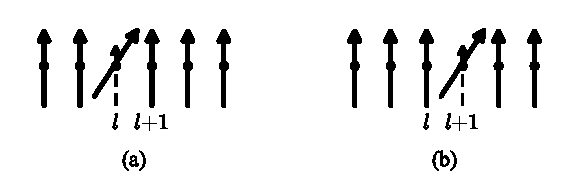
\includegraphics[width=7cm]{fig3-3.pdf}\\{\small 图 3.3}
\end{minipage}
\end{center}

哈密顿量 $H$ 中 $\hat{S}_l^{+}\hat{S}_{l+1}^{-}$ 项的作用使 $l$ 格点上偏转消失，而在 $(l+1)$
格点上产生新偏转[参看图3.3(b)]，状态 $|(S-1)_l\rangle$ 变为
\begin{equation*}
  |(S-1)_{l+1}\rangle=|S\rangle_1\cdots|S\rangle_l|S-1\rangle_{l+1}|S\rangle_{l+2}\cdots|S\rangle_N
\end{equation*}
偏转不再固定于 $l$ 格点上，它将在晶格中传播.这说明格点间的交换作用使得单个自旋偏转以集体激发的形式表现，与点阵位移在晶格中的传播相似.因此，在低激发态中少数自旋相对于量子化轴的偏离将因相互作用而被
$N$ 个自旋所平分.这时，每个自旋的平均偏离必然很小.

为了在数学上表示它们的相似性，也为了使 $H$ 对角化方便，我们引入量
\begin{equation}
  n\equiv S-m\qquad\left(m=0,\pm1,\cdots,\pm S\right)
\end{equation}
$n$ 代表自旋在量子化轴方向投影的偏离量，称为自旋偏离量子数.$n$ 取下列正整数：
\begin{equation}
  n=0,\ 1,\ 2,\ \cdots 2S\qquad\left(n\leqslant2S\right)
\end{equation}
与声子数相似.若用 $n$ 标记自旋态，则式(3.3.4)变换为
\begin{equation}
  \left.\begin{aligned}
    \hat{S}^{+}|n\rangle&=\sqrt{2S-(n-1)}\sqrt{n}\,|n-1\rangle\\
    \hat{S}^{-}|n\rangle&=\sqrt{2S-n}\sqrt{n+1}\,|n+1\rangle
  \end{aligned}\right\}
\end{equation}
显然，$\hat{S}^{+}$ 的作用使偏离趋于消灭，$\hat{S}^{-}$ 的作用为产生偏离.可以按常规引入对应于 $n$ 的产生和消灭算符
\begin{equation}
  a|n\rangle=\sqrt{n}\,|n-1\rangle,\qquad a^{+}|n\rangle=\sqrt{n+1}\,|n+1\rangle
\end{equation}
这时量子数 $n$ 的算符应为 $a^{+}a$，并且
\begin{equation}
  a^{+}a|n\rangle=n|n\rangle
\end{equation}
根据式(3.3.10)、(3.3.12)和(3.3.14)，容易找了下列算符变换关系：
\begin{equation}
  \left.\begin{aligned}
    \hat{S}^{+}&=\left(\sqrt{2S-a^{+}a}\right)a\\
    \hat{S}^{-}&=a^{+}\left(\sqrt{2S-a^{+}a}\right)\\
    \hat{S}^{z}&=\left(S-a^{+}a\right)
  \end{aligned}\right\}
\end{equation}
其中算符 $a$、$a^{+}$ 的对易式为
\begin{equation}
  \left[a,a^{+}\right]=1,\qquad\left[a,a\right]=\left[a^{+},a^{+}\right]=0
\end{equation}
下面将证明式(3.3.16)与自旋算符的对易式(3.3.3)是等价的.我们可以认为 $a^{+}$ 与 $a$
是玻色子的产生与消灭算符，唯一的差别只是这里的 $n$ 有限制，它不能超过 $2S$.

现在，由 $a$、$a^{+}$ 的对易式导出 $\hat{S}^{+}$、$\hat{S}^{-}$ 的对易式.
\begin{equation*}
\begin{aligned}
  \left[\hat{S}^{+},\hat{S}^{-}\right]&=\left(\sqrt{2S-a^{+}a}\right)aa^{+}\left(\sqrt{2S-a^{+}a}\right)
  -a^{+}\left(2S-a^{+}a\right)a\\
  &=\left(a^{+}a+1\right)\left(2S-a^{+}a\right)-a^{+}a\left(2S-a^{+}a\right)-a^{+}a\\
  &=2\left(S-a^{+}a\right)\\
  &=2\hat{S}^{z}
\end{aligned}
\end{equation*}
其中利用了 $\left[a^{+}a,a^{+}a\right]=0$ 和 $\left[a^{+}a,a\right]=-a$.

式(3.3.15)称为霍斯坦因－普里马可夫(Holstein-Primakoff)\textsuperscript{[5]}
变换，以后简称 HP 变换.将 HP 变换代入式(3.3.5)，得到海森伯哈密顿的二次量子化表示式
\begin{equation}
\begin{aligned}
  H=-J\sum_{l,\delta}^{\prime}\bigl\{&\left(S-a_l^{+}a_l\right)\left(S-a_{l+\delta}^{+}a_{l+\delta}\right)\\
  &+\frac{1}{2}\sqrt{2S-a_l^{+}a_l}\,a_l a_{l+\delta}^{+}\sqrt{2S-a_{l+\delta}^{+}a_{l+\delta}}\\
  &\left.+\frac{1}{2}a_l^{+}\sqrt{2S-a_l^{+}a_l}\sqrt{2S-a_{l+\delta}^{+}a_{l+\delta}}\,a_{l+\delta}\right\}
\end{aligned}
\end{equation}
算符的对易式可由式(3.3.16)推广得到
\begin{equation}
  \left[a_l,a_{l'}^{+}\right]=\delta_{l,l'},\qquad
  \left[a_l,a_{l'}\right]=\left[a_l^{+},a_{l'}^{+}\right]=0
\end{equation}
由于式(3.3.17)中含有偏离量子数 $n$ 所对应算符 $a^{+}a$ 的根号项，不仅使 $H$
的表示式变得十分复杂，而且对于激发态 $\left(n>0\right)$ 实际上无法求出 $H$ 的严格本征解，只能找近似解.所幸在低激发态每个自旋的平均偏离很小，这时可以将根号展开，并求得良好的低温近似解.

\subsection*{3. 低激发态——自旋波}

尽管式(3.3.17)比较复杂，但由于它用玻色粒子算符表示哈密顿量，将便于作低温展开使 $H$ 近似为可对角化的形式.

考虑与铁磁基态偏离不大的低激发态（即低温区），这时晶体中只有少数自旋发生了偏转，平均值
$\langle a_l^{+}a_l\rangle$ 应比 $2S$ 小得多，作为低阶近似可用 $\sqrt{2S}$
代替式(3.3.17)中的根号，再略去算符的四次方项，可将 $H$ 近似写为二次型
\begin{equation}
  H_0=-NZJS^2+2ZJS\sum_l a_l^{+}a_l
  -JS\sum_{l,\delta}^{\prime}\left(a_l a_{l+\delta}^{+}+a_l^{+}a_{l+\delta}\right)
\end{equation}
上式中第一项为基态能 $E_0$，第二项代表格点 $l$ 上的自旋偏离能，最后两项为不同格点间的耦合，它与简谐近似由位移表示的二次型哈密顿量相似.由于系统具有平移对称性，自旋的上升与下降算符
$\hat{S}_l^{\pm}$ 将与位移 $\boldsymbol{u}_l$ 相似，也可以用简正模
$N^{-\frac{1}{2}}\mathrm{e}^{-\mathrm{i}\boldsymbol{k}\cdot\boldsymbol{l}}$ 作展开表示 $\hat{S}_l^{\pm}$.再考虑到在低激态有近似关系
$\hat{S}_l^{+}=a_l\sqrt{2S}$ 及 $\hat{S}_l^{-}=a_l^{+}\sqrt{2S}$，可以设下列展开式：
\begin{equation}
  \left.\begin{aligned}
    a_l&=N^{-\frac{1}{2}}\sum_k\mathrm{e}^{\mathrm{i}\boldsymbol{k}\cdot\boldsymbol{l}}b_k\\
    a_l^{+}&=N^{-\frac{1}{2}}\sum_k\mathrm{e}^{-\mathrm{i}\boldsymbol{k}\cdot\boldsymbol{l}}b_k^{+}
  \end{aligned}\right\}
\end{equation}
这种类似于声子问题中引入简正坐标的办法，相当于对每个格点上的算符 $a_l$ 与 $a_l^{+}$
作点阵傅里叶变换.变换所引进的新算符由逆变换给出
\begin{equation}
  \left.\begin{aligned}
    b_k&=N^{-\frac{1}{2}}\sum_l\mathrm{e}^{-\mathrm{i}\boldsymbol{k}\cdot\boldsymbol{l}}a_l\\
    b_k^{+}&=N^{-\frac{1}{2}}\sum_l\mathrm{e}^{\mathrm{i}\boldsymbol{k}\cdot\boldsymbol{l}}a_l^{+}
  \end{aligned}\right\}
\end{equation}
显然，$b_k$ 与 $b_k^{+}$ 已不再是作用于某一格点上的算符，而是作用于所有格点的自旋波算符，代表自旋系统的集体坐标.新算符
$b_k$ 与 $b_k^{+}$ 同样满足玻色对易律
\begin{equation}
  \left.\begin{aligned}
    \left[b_k,b_{k'}^{+}\right]&=\delta_{kk'}\\
    \left[b_k,b_{k'}\right]&=\left[b_k^{+},b_{k'}^{+}\right]=0
  \end{aligned}\right\}
\end{equation}
将式(3.3.20)代入式(3.3.19)，再利用
$N^{-1}\sum_l\mathrm{e}^{\mathrm{i}\left(\boldsymbol{k}-\boldsymbol{k}'\right)\cdot\boldsymbol{l}}=\delta_{kk'}$，求得对角化的哈密顿量
\begin{equation}
\begin{aligned}
  H_0&=E_0+2ZJS\sum_k b_k^{+}b_k-ZJS\sum_k\gamma_k\left(b_kb_k^{+}+b_k^{+}b_k\right)\\
  &=E_0+\sum_k\hbar\omega_k b_k^{+}b_k
\end{aligned}
\end{equation}
$\omega_k$ 是自旋波频率，$\hbar\omega_k$ 代表自旋波的量子，简称为磁振子
\begin{equation}
  \hbar\omega_k=2ZJS\left(1-\gamma_k\right)
\end{equation}
其中定义了自旋波的结构因子
\begin{equation}
  \gamma_k=Z^{-1}\sum_\delta\mathrm{e}^{\mathrm{i}\boldsymbol{k}\cdot\boldsymbol{\delta}}=\gamma_{-k}
\end{equation}
$\gamma_k=\gamma_{-k}$ 是由于晶格有反演对称性，此外还有
\begin{equation}
  \sum_k\gamma_k=\sum_{\delta\neq0}\sum_k\frac{1}{Z}\mathrm{e}^{\mathrm{i}\boldsymbol{k}\cdot\boldsymbol{\delta}}=0
\end{equation}
不同结构晶体的 $\gamma_k$ 不同，因此求自旋波频率与波矢 $\boldsymbol{k}$
的关系时，应结合晶体对称性作计算.在低温情况下可利用长波条件
$\left|\boldsymbol{k}\cdot\boldsymbol{\delta}\right|<\!<1$ 展开 $\gamma_k$，求得 $\hbar\omega_k$ 的简单表示式
\begin{equation}
\begin{aligned}
  \hbar\omega_k&=2ZJS\left(1-\gamma_k\right)\\
  &\approx 2JS\biggl\{Z-\sum_\delta\biggl[1-\frac{1}{2}\left(\boldsymbol{k}\cdot\boldsymbol{\delta}\right)^2\biggr]\biggr\}\\
  &=JS\sum_\delta\left(\boldsymbol{k}\cdot\boldsymbol{\delta}\right)^2
\end{aligned}
\end{equation}
立方系的 3 种晶格（sc、bcc 和 fcc）有相同的长波色散关系
\begin{equation}
  \hbar\omega_k=2JSa^2k^2
\end{equation}
因为
$\sum_\delta\left(\boldsymbol{k}\cdot\boldsymbol{\delta}\right)^2
=\biggl\{\frac{1}{Z}\sum_\delta Z\delta^2\cos^2\theta\left(\boldsymbol{k},\boldsymbol{\delta}\right)\biggr\}k^2$，$\cos^2\theta\left(\boldsymbol{k},\boldsymbol{\delta}\right)$
的平均值为 $1/3$，$Z\delta^2$ 的平均值对 3 种晶格均为 $6a^2$，$a$ 是立方胞边长.

式(3.3.23)已将海森伯哈密顿变换为熟知的谐振子形式，其中 $b_k^{+}b_k=\hat{n}_k$
代表自旋波量子的数密度算符，其本征值即是在 $\boldsymbol{k}$
波矢自旋波上所激发自旋波量子的个数，而 $b_k^{+}$ 与 $b_k$
又称为自旋波量子的产生及消灭算符.与声子问题相似，用自旋波量子数表示的态向量
$|n_1,\cdots,n_N\rangle$ 是 $H_0$ 的本征向量，因此 $H_0$ 通常又称为自旋波近似的哈密顿量.

若展开式(3.3.17)中根号
\begin{equation}
  \sqrt{1-a^{+}a/2S}=1-\frac{1}{2}\left(\frac{a^{+}a}{2S}\right)+\frac{1}{8}\left(\frac{a^{+}a}{2S}\right)^2+\cdots
\end{equation}
计入算符的高阶项的影响，可得
\begin{equation}
  H=H_0+H_1+\cdots
\end{equation}
其中
\begin{equation}
  H_1=\frac{ZJ}{2N}\sum_{k,k',q}\left(\gamma_{k-q}+\gamma_{k'}-2\gamma_{k-q-k'}\right)
  b_{k-q}^{+}b_{k'+q}^{+}b_{k'}b_k
\end{equation}
代表自旋波之间的相互作用，它消灭 $\boldsymbol{k}$ 与 $\boldsymbol{k}'$ 量子并产生
$\boldsymbol{k}-\boldsymbol{q}$，$\boldsymbol{k}'+\boldsymbol{q}$ 量子，是典型的准粒子互作用项.

从式(3.3.19)不难看出，自旋波只是下列线性化运动方程的解
\begin{equation}
  \mathrm{i}\hbar\frac{\partial a_l}{\partial t}=\left[a_l,H_0\right]
  =2ZJSa_l-JS\sum_{\delta}^{\prime}\left(a_{l+\delta}+a_{l-\delta}\right)
\end{equation}
因为只需对上式作傅里叶变换，即可得到自旋波的算符方程
\begin{equation}
  \mathrm{i}\hbar\frac{\partial b_k}{\partial t}=2ZJS\left(1-\gamma_k\right)b_k=\hbar\omega_kb_k
\end{equation}
其中 $\hbar\omega_k$ 就是磁振子的能量，说明自旋波以 $\omega_k$
频率振荡.所以，前面求出的自旋波模式只是线性理论的结果，而磁振子可称为系统的线性元激发.如果进一步考虑自旋波之间的相互作用，我们将得到算符
$a_l$
的非线性方程.在一维情况下，这个非线性方程有孤子解，孤子代表系统的非线性元激发，我们将在本章§7中介绍.

自旋波之间的相互作用对于 $\omega_k$ 有重要的修正效应.若从 $H_0+H_1$ 出发，建立 $b_k$ 的运动方程
\begin{equation}
  \mathrm{i}\hbar\dot{b}_k=\left[b_k,H_0\right]+\left[b_k,H_1\right]
\end{equation}
再利用对易关系式(3.3.22)和 $H_0$ 及 $H_1$ 的表示式(3.3.23)和(3.3.31)，可算出
\begin{equation}
  \left[b_k,H_0\right]=2ZJS\left(1-\gamma_k\right)b_k
\end{equation}
\begin{equation}
\begin{aligned}
  \left[b_k,H_1\right]=\frac{ZJ}{2N}\sum_{k',q}\biggl\{&\left(\gamma_k+\gamma_{k'}-2\gamma_{k-k'}\right)
  b_{k'+q}^{+}b_{k+q}b_{k'}\\
  &+\left(\gamma_{k-q}+\gamma_{k'-q}-2\gamma_{k-k'}\right)b_{k'-q}^{+}b_{k-q}b_{k'}\biggr\}
\end{aligned}
\end{equation}
为了得到互作用项 $H_1$ 对于自旋波频谱的修正，对上式作线性化近似
\begin{equation}
  b_k^{+}b_{k_1}b_{k_2}\approx\left(\delta_{kk_1}b_{k_2}+\delta_{kk_2}b_{k_1}\right)\langle b_k^{+}b_k\rangle_T
\end{equation}
其中
\begin{equation}
  \langle b_k^{+}b_k\rangle_T=\left\{\mathrm{e}^{\hbar\omega_k/k_{\mathrm{B}}T}-1\right\}^{-1}
  =\langle\hat{n}_k\rangle_T
\end{equation}
再利用等式
\begin{equation*}
  \gamma_{k-k'}=\gamma_{k'-k}
\end{equation*}
和
\begin{equation}
  \sum_{k'}\gamma_{k-k'}\langle\hat{n}_{k'}\rangle_T=\gamma_k\sum_{k'}\gamma_{k'}\langle\hat{n}_{k'}\rangle_T
\end{equation}
经整理后得到下列线性方程
\begin{equation}
  \mathrm{i}\hbar\dot{b}_k=\hbar\omega_k\left(T\right)b_k
\end{equation}
求出修正后的自旋波量子与温度 $T$ 有关，其表示式为
\begin{equation}
  \hbar\omega_k\left(T\right)=2ZJS\left(1-\gamma_k\right)\left\{\frac{1-e\left(T\right)}{S}\right\}
\end{equation}
这里
\begin{equation}
  e\left(T\right)\equiv\frac{1}{N}\sum_{k'}\left(1-\gamma_{k'}\right)\langle\hat{n}_{k'}\rangle_T
\end{equation}
显然，相互作用对自旋波量子的修正归结为重正因子 $\left\{\frac{1-e\left(T\right)}{S}\right\}$
，这个因子随温度升高而减少，表明当温度升高时会发生自旋波频率的软化现象，从而导致失稳.具体计算
$\hbar\omega_k\left(T\right)$
时，应当联立式(3.3.38)、(3.3.41)和(3.3.42)自洽求解.图3.4
是铁磁绝缘材料 $\mathrm{EuO}$ 中 $\hbar\omega_k\left(T\right)$
的实验与理论比较\textsuperscript{[6]}，其中 $\square$、$\triangle$、$\circ$、$\bullet$
代表不同波矢自旋波量子的测量值，实线为上述理论的自洽解，显然两者符合较好.

\begin{center}
\begin{minipage}{8cm}
\centering
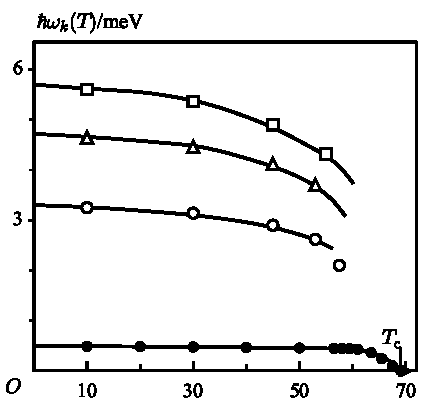
\includegraphics[width=8cm]{fig3-4.pdf}\\{\small
  图 3.4\quad $\mathrm{EuO}$ 的 $\hbar\omega_k(T)$ 曲线，$T_{\mathrm{c}}=69.1\ \mathrm{K}$\\
  $k=2\ \mathrm{nm}^{-1}(\bullet)$，$6\ \mathrm{nm}^{-1}(\circ)$，$8\ \mathrm{nm}^{-1}(\triangle)$，$10\ \mathrm{nm}^{-1}(\square)$}
\end{minipage}
\end{center}

\section{铁磁体的低温磁化强度}

由于自旋波算符满足玻色对易关系，因此温度为 $T$ 时 $\boldsymbol{k}$
自旋波所激发量子的平均数应按玻色分布决定，即
\begin{equation}
  \langle\hat{n}_k\rangle_T=\langle b_k^{+}b_k\rangle_T
  =\frac{1}{\mathrm{e}^{\hbar\omega_k/k_{\mathrm{B}}T}-1}
\end{equation}
低温时所有自旋波模的总元激发个数可利用式(3.3.28)写为
\begin{equation}
  \sum_k\langle\hat{n}_k\rangle_T=\frac{V}{8\pi^3}\int_{\Omega^{*}}
  \frac{\mathrm{d}^3k}{\exp\left[2SJa^2k^2/k_{\mathrm{B}}T\right]-1}
\end{equation}
设温度足够低，$2SJa^2k_{\mathrm{max}}^2>\!>k_{\mathrm{B}}T$，积分可以近似在全 $\boldsymbol{k}$ 空间进行，经整理后得
\begin{equation}
\begin{aligned}
  \frac{1}{N}\sum_k\langle\hat{n}_k\rangle_T
  &=\left(\frac{V}{2Na^3}\right)\cdot\left(\frac{k_{\mathrm{B}}T}{2JS}\right)^{3/2}
  \cdot\left(\frac{1}{2\pi^2}\int_0^{\infty}\frac{x^{\frac{1}{2}}\mathrm{d}x}{\mathrm{e}^{x}-1}\right)\\
  &=\left(\frac{V}{2Na^3}\right)\cdot\left(\frac{k_{\mathrm{B}}T}{2JS}\right)^{3/2}
  \cdot\frac{1}{2\pi^2}\Gamma\left(\frac{3}{2}\right)\zeta\left(\frac{3}{2}\right)\\
  &=\left(\frac{k_{\mathrm{B}}T}{2SJ}\right)^{3/2}\alpha
\end{aligned}
\end{equation}
其中 $x\equiv\left(2SJa^2k^2/k_{\mathrm{B}}T\right)$，$\Gamma\left(\frac{3}{2}\right)=\frac{1}{2}\sqrt{\pi}$
，而黎曼函数 $\zeta\left(\frac{3}{2}\right)=2.612$.
对于 sc、bcc 和 fcc 晶格 $\left(\frac{V}{2Na^3}\right)$ 分别为
$\frac{1}{2}$、$\frac{1}{4}$ 和 $\frac{1}{8}$，因此 $\alpha$ 分别等于
$\frac{0.117}{2}$(sc)、$\frac{0.117}{4}$(bcc) 和 $\frac{0.117}{8}$(fcc).
当取体积 $V=1$ 时，铁磁体的低温磁化强度为
\begin{equation}
\begin{aligned}
  M\left(T\right)&=g\mu_{\mathrm{B}}\sum_l\left(S-\langle a_l^{+}a_l\rangle_T\right)\\
  &=Ng\mu_{\mathrm{B}}S-g\mu_{\mathrm{B}}\sum_k\left(\langle b_k^{+}b_k\rangle_T\right)\\
  &=M\left(0\right)\left\{1-\frac{1}{NS}\sum_k\langle\hat{n}_k\rangle_T\right\}\\
  &=M\left(0\right)\left\{1-\frac{\alpha}{S}\left(\frac{k_{\mathrm{B}}T}{2SJ}\right)^{3/2}\right\}
\end{aligned}
\end{equation}
其中 $M\left(0\right)=Ng\mu_{\mathrm{B}}S$
代表零温饱和磁化.由于自旋波激发所引起磁化强度的减小为
\begin{equation}
\begin{aligned}
  \Delta M\left(T\right)&=M\left(0\right)-M\left(T\right)\\
  &=M\left(0\right)\frac{\alpha}{S}\left(\frac{k_{\mathrm{B}}T}{2SJ}\right)^{3/2}\sim T^{3/2}
\end{aligned}
\end{equation}
这个结果是布洛赫\textsuperscript{[7]}最早求得的，其形式与实验得到的相同，称为布洛赫 $T^{3/2}$ 定律.

众所周知，用平均场理论求出的低温磁化强度为
\begin{equation}
  M\left(T\right)=M\left(0\right)\left\{1-\frac{1}{S}\mathrm{e}^{-\frac{3T_{\mathrm{c}}}{\left(S+1\right)T}}\right\}
\end{equation}
其中 $T_{\mathrm{c}}$ 为铁磁体的居里温度，
\begin{equation}
  T_{\mathrm{c}}=\frac{2}{3}\frac{ZJ}{k_{\mathrm{B}}}S\left(S+1\right)
\end{equation}
显然，平均场的结果表明 $\Delta M\left(T\right)$
按指数衰数，显然与实验不符.现在分析低温下平均场理论失败的原因.平均场理论将 $l$
格点自旋受到其它格点上自旋的海森伯交换作用近似为
\begin{equation}
  \mathcal{H}_l\approx-2\hat{\boldsymbol{S}}_l\cdot\biggl\{\sum_{l'}J_{ll'}\langle\hat{\boldsymbol{S}}_{l'}\rangle\biggr\}
\end{equation}
这里将 $\hat{\boldsymbol{S}}_{l'}$ 算符用平均值代替，从而定义了一个有效磁场 $\boldsymbol{h}_{\mathrm{eff}}$
\begin{equation}
  g\mu_{\mathrm{B}}\boldsymbol{h}_{\mathrm{eff}}\equiv2\sum_{l'}J_{ll'}\langle\hat{\boldsymbol{S}}_{l'}\rangle
  \approx2ZJ\langle\hat{\boldsymbol{S}}\rangle
\end{equation}
其中 $Z$ 为配位数，$g$ 是朗德因子，$\mu_{\mathrm{B}}$
是玻尔磁子，并考虑到铁磁体各格点上是相同自旋的离子，可略去平均量 $\langle\hat{\boldsymbol{S}}_l\rangle$ 的
$l$ 脚标.由于磁化强度 $\boldsymbol{M}=Ng\mu_{\mathrm{B}}\langle\hat{\boldsymbol{S}}\rangle$，因此
$\boldsymbol{h}_{\mathrm{eff}}\sim\boldsymbol{M}$，它就是外斯分子场.
式(3.4.8)称为海森伯互作用的平均场近似，它使多自旋互作用问题简化为平均场中的单自旋运动.这时任一自旋的哈密顿量为
\begin{equation*}
  \mathcal{H}=-\lambda g\mu_{\mathrm{B}}\hat{S}^{z}M
  \left[\lambda=\frac{2ZJ}{N\left(g\mu_{\mathrm{B}}\right)^2}\right]
\end{equation*}
其本征值为
\begin{equation}
  E_m=-\lambda g\mu_{\mathrm{B}}m\,M\qquad\left(m=0,\pm1,\cdots,\pm S\right)
\end{equation}
磁化强度为
\begin{equation}
  M\left(T\right)=Ng\mu_{\mathrm{B}}\langle\hat{S}^{z}\rangle
  =Ng\mu_{\mathrm{B}}\frac{\displaystyle\sum_{m=-S}^{S}m\,\mathrm{e}^{-\beta E_m}}
  {\displaystyle\sum_{m=-S}^{S}\mathrm{e}^{-\beta E_m}}
  =M\left(0\right)B_s(x)\quad\left[\beta=\left(k_{\mathrm{B}}T\right)^{-1}\right]
\end{equation}
这里布里渊函数
\begin{equation}
\begin{aligned}
  B_s\left(x\right)&=\left(\frac{2S+1}{2S}\right)\coth\biggl\{\left(\frac{2S+1}{2S}\right)x\biggr\}
  -\frac{1}{2S}\coth\biggl\{\left(\frac{1}{2S}\right)x\biggr\}\\
  &\qquad\qquad\left(x=\lambda g\mu_{\mathrm{B}}\frac{SM}{k_{\mathrm{B}}T}\right)
\end{aligned}
\end{equation}
利用高温展开式
\begin{equation}
  B_s\left(x\right)\approx\frac{S+1}{S}\,\frac{x}{3}\qquad\left(x<\!<1\right)
\end{equation}
可确定居里温度 $T_{\mathrm{c}}$ 与交换积分 $J$
的关系，求得式(3.4.7).当 $T<\!<T_{\mathrm{c}}$ 时，利用低温展开式
\begin{equation}
  B_s\left(x\right)\approx1-\frac{1}{S}\mathrm{e}^{-\frac{x}{S}}\qquad
  \left(\mathrm{e}^{-\frac{x}{S}}<\!<1\right)
\end{equation}
可导出平均场的低温 $M(T)$ 公式(3.4.6).显然，平均场理论只考虑了自旋运动的单体效应，它不能反映低温区自旋系统的集体激发特征.集体激发是多体效应，涉及自旋关联，其具体表现为：当任一自旋受其它
$(N-1)$ 个自旋作用而改变取向时，其它自旋的取向也将同时变化，这是海森伯互作用
$\hat{\boldsymbol{S}}_l\cdot\hat{\boldsymbol{S}}_{l'}$
算符特性的表现，称为自旋间的动力学关联.平均场理论在低温区失效的原因就是由于忽略了动力学关联，而自旋波理论则考虑了这种关联，所以取得了成功.

此外，容易算出铁磁体中磁振子的低温比热容
\begin{equation}
  c_m=\nu Nk_{\mathrm{B}}\left(\frac{k_{\mathrm{B}}T}{2JS}\right)^{3/2}
\end{equation}
其中常数 $\nu$ 对于 sc、bcc 和 fcc 晶格分别为 0.113、0.113/2 和 0.113/4.

在结束本节之前，我们还将导出自旋波的经典图像，根据对角化的哈密顿量式(3.3.23)，易求出
$\boldsymbol{k}$ 模自旋波算符的含时解为
$b_k\left(t\right)=b_k\left(0\right)\mathrm{e}^{-\mathrm{i}\omega_kt}$
，代入式(3.3.20)可将每个格点的自旋偏离算符写成
\begin{equation}
  \left.\begin{aligned}
    a_l\left(t\right)&=N^{-\frac{1}{2}}\sum_kb_k\left(0\right)
    \mathrm{e}^{\mathrm{i}\left(\boldsymbol{k}\cdot\boldsymbol{l}-\omega_kt\right)}\\
    a_l^{+}\left(t\right)&=N^{-\frac{1}{2}}\sum_kb_k^{+}\left(0\right)
    \mathrm{e}^{-\mathrm{i}\left(\boldsymbol{k}\cdot\boldsymbol{l}-\omega_kt\right)}
  \end{aligned}\right\}
\end{equation}
再考虑到在低激发态可以将自旋的上升与下降算符分别用 $a_l\sqrt{2S}$ 与
$a_l^{+}\sqrt{2S}$ 近似表示，这时低激发态的自旋振荡解为
\begin{equation}
  \left.\begin{aligned}
    \hat{S}_l^{+}\left(t\right)&=\sqrt{\frac{2S}{N}}\sum_kb_k\left(0\right)
    \mathrm{e}^{\mathrm{i}\left(\boldsymbol{k}\cdot\boldsymbol{l}-\omega_kt\right)}\\
    \hat{S}_l^{-}\left(t\right)&=\sqrt{\frac{2S}{N}}\sum_kb_k^{+}\left(0\right)
    \mathrm{e}^{\mathrm{i}\left(\boldsymbol{k}\cdot\boldsymbol{l}-\omega_kt\right)}
  \end{aligned}\right\}
\end{equation}
对上式作经典近似，将算符 $b_k\left(0\right)$ 与 $b_k^{+}\left(0\right)$
取为实 c 数，相应的将上升、下降算符 $\hat{\boldsymbol{S}}_l^{\pm}$
看成是经典矢量 $\boldsymbol{S}_l$ 的横向分量 $S_l^{\pm}$，再利用
$S_l^{x}=\frac{1}{2}\left(S_l^{+}+S_l^{-}\right)$ 及
$S_l^{y}=\frac{1}{2\mathrm{i}}\left(S_l^{+}-S_l^{-}\right)$，求出
$\boldsymbol{k}$ 模自旋波的经典近似解
\begin{equation}
  \left.\begin{aligned}
    S_l^{x}\left(t\right)&\sim\cos\left(\boldsymbol{k}\cdot\boldsymbol{l}-\omega_kt\right)\\
    S_l^{y}\left(t\right)&\sim\sin\left(\boldsymbol{k}\cdot\boldsymbol{l}-\omega_kt\right)
  \end{aligned}\right\}
\end{equation}
显然，上式表明：任一格点上的自旋都可以看成是经典的矢量，它们在 $Oxy$
平面内作圆周运动，并且相邻格点之间有确定的相位差（由 $\boldsymbol{k}\cdot\boldsymbol{l}$
决定），正如图3.2(b)所示.这就是图3.2中自旋波经典图像的来源.

\section{反铁磁自旋波理论}

当海森伯哈密顿量中 $J<0$ 时，近邻格点上的自旋趋于反平行排列，这时往往可以把晶格分为两个子格，在每个子格中自旋平行排列与铁磁情况一样，但两个子格的自旋取向相反，因此总的自发磁化相互抵消，这就是反铁磁体的双子格模型.例如在反铁磁材料
$\mathrm{MnF}_2$、$\mathrm{FeF}_2$ 和 $\mathrm{CoF}_2$
中，磁离子（$\mathrm{Mn}^{2+}$、$\mathrm{Fe}^{2+}$ 和
$\mathrm{Co}^{2+}$）排成体心四方晶格，它们可划分为两个简单四方子格.

\subsection*{1. 双子格模型}

我们将从双子格模型出发，讨论海森伯哈密顿量的基态和激发态.设每个子格中自旋数为 $N$，总的磁离子数为
$2N$，并取体积 $V=1$.$H$ 用 $a$、$b$ 两子格的自旋符表示
\begin{equation}
\begin{aligned}
  H={}&\left|J\right|\sum_{i,\delta}\biggl\{\hat{S}_{ai}^{z}\hat{S}_{b,i+\delta}^{z}
  +\frac{1}{2}\left(\hat{S}_{ai}^{+}\hat{S}_{b,i+\delta}^{-}+\hat{S}_{ai}^{-}\hat{S}_{b,i+\delta}^{+}\right)\biggr\}\\
  &+\left|J\right|\sum_{j,\delta}\biggl\{\hat{S}_{bj}^{z}\hat{S}_{a,j+\delta}^{z}
  +\frac{1}{2}\left(\hat{S}_{bj}^{+}\hat{S}_{a,j+\delta}^{-}+\hat{S}_{bj}^{-}\hat{S}_{a,j+\delta}^{+}\right)\biggr\}
\end{aligned}
\end{equation}
其中 $\hat{\boldsymbol{S}}_{ai}$ 代表子格 $a$ 中 $i$
格点上自旋算符，$\hat{\boldsymbol{S}}_{bj}$ 为 $b$ 子格中 $j$
格点上自旋.假设子格 $a$ 的量子化轴沿 $(+z)$ 方向，$b$ 沿 $(-z)$
方向，我们将所有 $a$ 子格中自旋沿 $(+z)$ 向排列，$b$ 中沿 $(-z)$
向排列的状态[如图3.1(b)]称为出发状态 $|\mathrm{Origin}\rangle$，则存在着与式(3.3.7)相似的关系
\begin{equation}
  \hat{S}_{ai}^{+}|\mathrm{Origin}\rangle=\hat{S}_{bj}^{-}|\mathrm{Origin}\rangle=0
\end{equation}
它说明 $\hat{S}_{ai}^{+}$ 对应于子格 $a$ 中的消灭算符，$\hat{S}_{bj}^{-}$
对应于 $b$ 子格的消灭算符，由于 $a$
子格自旋朝上，可仿铁磁情况作霍斯坦因－普里马可夫变换引入子格 $a$ 的产生及消灭算符
\begin{equation}
  \left.\begin{aligned}
    \hat{S}_{ai}^{+}&=\left(\sqrt{2S-a_i^{+}a_i}\right)a_i\\
    \hat{S}_{ai}^{-}&=a_i^{+}\sqrt{2S-a_i^{+}a_i}\\
    \hat{S}_{ai}^{z}&=S-a_i^{+}a_i
  \end{aligned}\right\}
\end{equation}
对于 $b$ 子格 $\hat{\boldsymbol{S}}^{+}$ 与 $\hat{\boldsymbol{S}}^{-}$ 的作用将颠倒，应定义
\begin{equation}
  \left.\begin{aligned}
    \hat{S}_{bj}^{+}&=b_j^{+}\sqrt{2S-b_j^{+}b_j}\\
    \hat{S}_{bj}^{-}&=\left(\sqrt{2S-b_j^{+}b_j}\right)b_j\\
    \hat{S}_{bj}^{z}&=b_j^{+}b_j-S
  \end{aligned}\right\}
\end{equation}
由于 $b$
子格的自旋上升是相对于量子化轴 $(-z)$ 的偏离增大，因此 $\hat{\boldsymbol{S}}_b^{+}$
对应于产生算符 $b^{+}$，$b$ 子格中 $\hat{\boldsymbol{S}}_b^{z}$
的定义与 $a$
子格相差负号的原因也是类似的，它可以从对易关系证明
\begin{equation*}
\begin{aligned}
  \left[\hat{S}_{bj}^{+},\hat{S}_{bj}^{-}\right]&=b_j^{+}\sqrt{2S-b_j^{+}b_j}\sqrt{2S-b_j^{+}b_j}\,b_j
  -\left(\sqrt{2S-b_j^{+}b_j}\right)b_jb_j^{+}\left(\sqrt{2S-b_j^{+}b_j}\right)\\
  &=b_j^{+}b_j\left(2S-b_j^{+}b_j\right)+b_j^{+}b_j
  -b_j^{+}b_j\left(2S-b_j^{+}b_j\right)-\left(2S-b_j^{+}b_j\right)\\
  &=2\left(b_j^{+}b_j-S\right)
\end{aligned}
\end{equation*}
与 $\left[\hat{S}_{bj}^{+},\hat{S}_{bj}^{-}\right]=2\hat{S}_{bj}^{z}$
相比较，可得式(3.5.4)的第 3 个等式.

$a_i$、$b_j$ 都是玻色算符，它们满足对易关系
\begin{equation}
\begin{aligned}
  &\left[a_i,a_{i'}^{+}\right]=\delta_{ii'},\qquad
  \left[a_i,a_{i'}\right]=\left[a_i^{+},a_{i'}^{+}\right]=0\\
  &\left[b_j,b_{j'}^{+}\right]=\delta_{jj'},\qquad
  \left[b_j,b_{j'}\right]=\left[b_j^{+},b_{j'}^{+}\right]=0\\
  &\left[a_i,b_j\right]=\left[a_i^{+},b_j\right]=\left[a_i,b_j^{+}\right]=\left[a_i^{+},b_j^{+}\right]=0
\end{aligned}
\end{equation}
对于低激发态，可用下列近似：
\begin{equation}
\begin{aligned}
  &\hat{S}_{ai}^{+}=(2S)^{\frac{1}{2}}a_i,\qquad
  \hat{S}_{ai}^{-}=(2S)^{\frac{1}{2}}a_i^{+},\qquad
  \hat{S}_{ai}^{z}=S-a_i^{+}a_i\\
  &\hat{S}_{bj}^{+}=(2S)^{\frac{1}{2}}b_j^{+},\qquad
  \hat{S}_{bj}^{-}=(2S)^{\frac{1}{2}}b_j,\qquad
  \hat{S}_{bj}^{z}=b_j^{+}b_j-S
\end{aligned}
\end{equation}
代入式(3.5.1)，并略去 $\hat{\boldsymbol{S}}_a^{z}\hat{\boldsymbol{S}}_b^{z}$
中算符 $a$、$b$ 的四次项，求得低温近似的哈密顿量
\begin{equation}
\begin{aligned}
  H={}&-2NZS^2\left|J\right|+2ZS\left|J\right|\biggl(\sum_i a_i^{+}a_i+\sum_j b_j^{+}b_j\biggr)\\
  &+2\left|J\right|S\sum_{i,\delta}\left(a_ib_{i+\delta}+a_i^{+}b_{i+\delta}^{+}\right)
\end{aligned}
\end{equation}
其中 $N$ 为子格中自旋数.仿照铁磁情况作傅里叶变换，分别对各子格引入自旋波算符 $a_k$、$b_k$：
\begin{equation}
  \left.\begin{aligned}
    a_i&=N^{-\frac{1}{2}}\sum_k\mathrm{e}^{\mathrm{i}\boldsymbol{k}\cdot\boldsymbol{R}_i}a_k\,,&
    a_i^{+}&=N^{-\frac{1}{2}}\sum_k\mathrm{e}^{-\mathrm{i}\boldsymbol{k}\cdot\boldsymbol{R}_i}a_k^{+}\\
    b_j&=N^{-\frac{1}{2}}\sum_k\mathrm{e}^{-\mathrm{i}\boldsymbol{k}\cdot\boldsymbol{R}_j}b_k\,,&
    b_j^{+}&=N^{-\frac{1}{2}}\sum_k\mathrm{e}^{\mathrm{i}\boldsymbol{k}\cdot\boldsymbol{R}_j}b_k^{+}
  \end{aligned}\right\}
\end{equation}
$\boldsymbol{R}_i$、$\boldsymbol{R}_j$ 为子格 $a$、$b$
的矢量，变换后的算符 $a_k$、$b_k$ 分别满足玻色对易关系
\begin{equation}
  \left[a_k,a_{k'}^{+}\right]=\left[b_k,b_{k'}^{+}\right]=\delta_{kk'}
\end{equation}
其它的对易式均等于零，算符 $a_k$ 与 $b_k$ 之间也可对易：
\begin{equation}
  \left[a_k,b_{k'}\right]=\left[a_k,b_{k'}^{+}\right]=\left[a_k^{+},b_{k'}\right]=\left[a_k^{+},b_{k'}^{+}\right]=0
\end{equation}
用双子格自旋波算符表示的哈密顿量为
\begin{equation}
\begin{aligned}
  H={}&-2NZS^2\left|J\right|+2ZS\left|J\right|\sum_k\left(a_k^{+}a_k+b_k^{+}b_k\right)\\
  &+2ZS\left|J\right|\sum_k\gamma_k\left(a_k^{+}b_k^{+}+b_ka_k\right)
\end{aligned}
\end{equation}
上式中第一项是出发状态的能量，第二项代表各子格中自旋波，第三项为交叉项代表两子格自旋波的相互作用.
式(3.5.11)说明本征模式应当是两个子格自旋波的组合.我们必须进一步作变换，引入组合的自旋波算符，才能消除交叉项，使
$H$ 对角化.

\subsection*{2. 玻戈留玻夫正则变换}

如何组合两个子格中的自旋波算符？让我们先考察子格算符的运动方程
\begin{equation}
  \left.\begin{aligned}
    \mathrm{i}\hbar\dot{a}_k&=\left[a_k,H\right]=2ZS\left|J\right|\left(a_k+\gamma_kb_k^{+}\right)\\
    \mathrm{i}\hbar\dot{b}_k&=\left[b_k,H\right]=2ZS\left|J\right|\left(b_k+\gamma_ka_k^{+}\right)
  \end{aligned}\right\}
\end{equation}
上式说明，应当组合 $a_k$ 与 $b_k^{+}$ 以及 $b_k$ 与 $a_k^{+}$
构成两套新的自旋波算符 $\alpha_k$ 和 $\beta_k$
\begin{equation}
  \left.\begin{aligned}
    \alpha_k&=u_ka_k-v_kb_k^{+}\ ,&\quad \alpha_k^{+}&=u_ka_k^{+}-v_kb_k\\
    \beta_k&=u_kb_k-v_ka_k^{+}\ ,&\quad \beta_k^{+}&=u_kb_k^{+}-v_ka_k
  \end{aligned}\right\}
\end{equation}
这里 $u_k$ 和 $v_k$ 设为实函数，式(3.5.13)为正则变换.应当指出，作正则变换时要保证所有的对易关系在形式上不改变，这是检验变换式(3.5.13)的一个重要物理条件.

由于要求变换后新算符仍满足玻色对易式
\begin{equation}
  \left[\alpha_k,\alpha_{k'}^{+}\right]=\delta_{kk'}\ ,\qquad
  \left[\beta_k,\beta_{k'}^{+}\right]=\delta_{kk'}
\end{equation}
可求得 $u_k$ 与 $v_k$ 的一个关系式
\begin{equation}
  u_k^2-v_k^2=1
\end{equation}
再要求用新算符 $\alpha_k$、$\beta_k$ 表示的哈密顿量 $H$
对角化，将得到 $u_k$ 与 $v_k$
的另一个关系式，从而具体解出 $u_k$ 与
$v_k$.这就是著名的玻戈留玻夫(N.N.Bogoliubov)变换\textsuperscript{[9]}
，它已成功用于超流、声子-光子、声子-自旋波等一系列耦合问题.

不难验证，变换式(3.5.13)保证了对易关系不变，新算符 $\alpha$ 与 $\beta$ 之间是可对易的，即
\begin{equation}
  \left[\alpha_k,\beta_{k'}\right]=\left[\alpha_k,\beta_{k'}^{+}\right]
  =\left[\alpha_k^{+},\beta_{k'}\right]=\left[\alpha_k^{+},\beta_{k'}^{+}\right]=0
\end{equation}
利用式(3.5.15)不难写出式(3.5.13)的逆变换
\begin{equation}
  \left.\begin{aligned}
    a_k&=u_k\alpha_k+v_k\beta_k^{+}\ ,&\quad a_k^{+}&=u_k\alpha_k^{+}+v_k\beta_k\\
    b_k&=u_k\beta_k+v_k\alpha_k^{+}\ ,&\quad b_k^{+}&=u_k\beta_k^{+}+v_k\alpha_k
  \end{aligned}\right\}
\end{equation}
代入式(3.5.11)得
\begin{equation}
\begin{aligned}
  H={}&-2NZ\left|J\right|S\left(S+1\right)\\
  &+2Z\left|J\right|S\sum_k\biggl\{\left(u_k^2+v_k^2+2\gamma_ku_kv_k\right)
  \left(\alpha_k^{+}\alpha_k+\beta_k^{+}\beta_k+1\right)\\
  &\qquad\left.+\left[\left(u_k^2+v_k^2\right)\gamma_k+2u_kv_k\right]
  \left(\alpha_k\beta_k+\alpha_k^{+}\beta_k^{+}\right)\right\}
\end{aligned}
\end{equation}
为使 $H$ 对角化，要求非对角项 $\left(\alpha_k\beta_k+\alpha_k^{+}\beta_k^{+}\right)$ 的系数等于零，即
\begin{equation}
  \left(u_k^2+v_k^2\right)\gamma_k+2u_kv_k=0
\end{equation}
上式与式(3.5.15)联立可解出
\begin{equation}
\begin{aligned}
  u_k^2&=\frac{1}{2}\left(1+\Delta\right)\\
  v_k^2&=-\frac{1}{2}\left(1-\Delta\right)\\
  \Delta&=\frac{1}{\sqrt{1-\gamma_k^2}}
\end{aligned}
\end{equation}
将此结果代入式(3.5.18)，求得对角化哈密顿量
\begin{equation}
\begin{aligned}
  H={}&-2NZ\left|J\right|S\left(S+1\right)\\
  &+\sum_k\hbar\omega_k\biggl\{\left(\alpha_k^{+}\alpha_k+\frac{1}{2}\right)
  +\left(\beta_k^{+}\beta_k+\frac{1}{2}\right)\biggr\}
\end{aligned}
\end{equation}
其中 $\hbar\omega_k$ 代表反铁磁自旋波量子
\begin{equation}
  \hbar\omega_k=2Z\left|J\right|S\sqrt{1-\gamma_k^2}
\end{equation}
由式(3.5.21)可以看出，对于每个 $\boldsymbol{k}$
存在两支简并的反铁磁自旋波，分别由 $\alpha_k^{+}\alpha_k$ 和
$\beta_k^{+}\beta_k$ 代表其准粒子数算符.

在长波限 $\left(ka<\!<1\right)$ 立方晶系的色散关系为
\begin{equation}
  \hbar\omega_k=2\left(2Z\right)^{\frac{1}{2}}S\left|J\right|ka
\end{equation}
反铁磁自旋波的频率是 $k$
的线性函数，与声学模声子的长波色散关系相同.由此不难求出反铁磁体中磁振子的比热正比于
$T^3$，和德拜声子的比热相似.

例如反铁磁体的低温磁振子比热.

反铁磁体中由于激发自旋波量子，在温度 $T$ 时磁振子的内能为
\begin{equation}
\begin{aligned}
  U\left(T\right)&=\sum_k\langle\alpha_k^{+}\alpha_k\rangle_T\hbar\omega_k
  +\sum_k\langle\beta_k^{+}\beta_k\rangle_T\hbar\omega_k\\
  &=2\sum_k\frac{\hbar\omega_k}{\exp\left(\dfrac{\hbar\omega_k}{k_{\mathrm{B}}T}\right)-1}
\end{aligned}
\end{equation}
考虑两个简立方的子格（边长为 $a$）相互穿插构成 bcc 晶格.
当 $\hbar\omega_k>\!>k_{\mathrm{B}}T$ 时，利用式(3.5.23)，求得内能的近似式为
\begin{equation}
\begin{aligned}
  U\left(T\right)&=\frac{2Na^3}{8\pi^3}\,4\pi\int_0^{\infty}
  \frac{\hbar\omega_k\,k^2\mathrm{d}k}{\exp\left(\dfrac{\hbar\omega_k}{k_{\mathrm{B}}T}\right)-1}\\
  &=\frac{2N\left(k_{\mathrm{B}}T\right)^4}{2\pi^2\left\{2S\left|J\right|\left(2Z\right)^{\frac{1}{2}}\right\}^3}
  \int_0^{\infty}x^3\left(\mathrm{e}^{-x}+\mathrm{e}^{-2x}+\cdots\right)\mathrm{d}x
\end{aligned}
\end{equation}
磁振子的低温比热容可由 $U\left(T\right)$ 求出
\begin{equation}
  c_m=\frac{\partial U}{\partial T}=13.7\,k_{\mathrm{B}}\left(\frac{k_{\mathrm{B}}T}{12\left|J\right|S}\right)^3
\end{equation}
$c_m\propto T^3$，与实验测量一致.

\subsection*{3. 磁振子的零点运动}

现在讨论反铁磁体的基态，基态能量 $E_0$
应当是无准粒子激发时 $H$ 的本征值，根据式(3.5.21)和(3.5.22)
\begin{equation}
\begin{aligned}
  E_0&=-2NZ\left|J\right|S\left(S+1\right)+\sum_k\hbar\omega_k\\
  &=-2NZ\left|J\right|S\left(S+\lambda\right)
\end{aligned}
\end{equation}
其中
\begin{equation}
  \lambda=\frac{1}{N}\sum_k\left(1-\sqrt{1-\gamma_k^2}\right)
\end{equation}
由于 $\left|\gamma_k\right|<1$，故 $0<\lambda<1$.反铁磁体的基态能量介乎出发状态
$|\mathrm{Origin}\rangle$ 的能量 $\left(-2NZ\left|J\right|S^2\right)$ 与
$\left\{-2NZ\left|J\right|S\left(S+1\right)\right\}$
之间，安德逊\textsuperscript{[10]}用数值方法算得简立方自旋晶格的
$\lambda=0.58$
，说明基态并不完全像双子格模型所建议的磁有序状态[图3.1(b)].
在基态每一子格中自旋不是完全平行的，而是存在着取向的不一致性.

为使图像明确，我们将讨论子格的饱和磁化强度.子格总自旋的 $z$ 分量算符可表示为
\begin{equation*}
\begin{aligned}
  \hat{\mathcal{S}}_a^{z}\equiv\sum_{i=1}^{N}\hat{S}_{ai}^{z}
  &=\sum_{i=1}^{N}\left(S-a_i^{+}a_i\right)=NS-\sum_ka_k^{+}a_k\\
  &=N\biggl\{S-\frac{1}{N}\sum_k\left[u_k^2\alpha_k^{+}\alpha_k
  +v_k^2\beta_k\beta_k^{+}+u_kv_k\left(\alpha_k\beta_k+\alpha_k^{+}\beta_k^{+}\right)\right]\biggr\}
\end{aligned}
\end{equation*}
由于在 $\hat{\mathcal{S}}_a^{z}$ 中还存在非对角项，它不能与 $H$
同时对角化，我们只可以算出 $\hat{\mathcal{S}}_a^{z}$ 的基态平均值
\begin{equation}
\begin{aligned}
  \langle\hat{\mathcal{S}}_a^{z}\rangle_0
  &=N\biggl\{S-\frac{1}{N}\sum_kv_k^2\langle0\mid\beta_k\beta_k^{+}\mid0\rangle\biggr\}\\
  &=NS-\sum_kv_k^2
\end{aligned}
\end{equation}
上式右边第一项代表子格 $a$
中所有自旋取向完全一致时的贡献，对应于子格的饱和磁化.第二项为子格中自旋取向的平均偏离量
\begin{equation}
  \Delta\mathcal{S}_a^{z}\equiv NS-\langle\hat{\mathcal{S}}_a^{z}\rangle=\sum_kv_k^2
  =\frac{1}{2}\sum_k\biggl\{\frac{1}{\sqrt{1-\gamma_k^2}}-1\biggr\}
\end{equation}
安德逊算出简立方晶格的 $\Delta\mathcal{S}_a^{z}=0.078\,N$
.由此可知在基态中子格的自旋并非绝对取向一致，而是相对饱和值 $NS$
有少量的平均偏离，这种取向的无序性与反铁磁体中自旋波量子的零点运动有关.读者只需比较反铁磁的与铁磁体的哈密顿量式(3.5.21)和(3.5.23)，就可以看出反铁磁体与铁磁体不同之处是存在着磁振子的零点能，因此式(3.5.30)又称为子格自旋的零点偏离.

综上所述，我们只知道反铁磁体的基态相对于 $|\mathrm{Origin}\rangle$
有偏离，但 $|\mathrm{Origin}\rangle$
不是基态，甚至不是 $H$
的本征态.至于基态中各子格自旋具体如何排列，目前尚无法详细确定.因为
$\hat{\mathcal{S}}_a^{z}$、$\hat{\mathcal{S}}_b^{z}$ 与哈密顿量 $H$
不对易，$\left[H,\hat{\mathcal{S}}_a^{z}\right]\neq0$，
$\left[H,\hat{\mathcal{S}}_b^{z}\right]\neq0$.
所以，至今三维反铁磁海森伯模型的严格基态尚未找到.

\subsection*{4. 外场影响}

在磁性材料中实际上还存在各向异性晶体场，反铁磁体中的晶场可近似为
$\pm\boldsymbol{B}_{\mathrm{A}}$，对 $a$ 子格取正号，$b$
子格取负号.正是由于 $\boldsymbol{B}_{\mathrm{A}}$
的存在，使 $a$ 子格自旋沿 $(+z)$ 向和 $b$
子格自旋沿 $(-z)$
向排列的反铁磁序结构得以稳定.因此，当沿 $z$
轴方向存在外磁场 $\boldsymbol{B}$ 时，反铁磁体的塞曼(Zeeman)能项为
\begin{equation}
  \Delta H=-g\mu_{\mathrm{B}}\left(\boldsymbol{B}+\boldsymbol{B}_{\mathrm{A}}\right)\sum_i\hat{S}_{ai}^{z}
  -g\mu_{\mathrm{B}}\left(\boldsymbol{B}-\boldsymbol{B}_{\mathrm{A}}\right)\sum_j\hat{S}_{bj}^{z}
\end{equation}
对上式作霍斯坦因－普里马可夫变换和傅里叶变换后再与式(3.5.11)相加，构成有外场时反铁磁自旋波的哈密顿量为
\begin{equation}
  H=E_0+\sum_k\left\{\left(\xi+g\mu_{\mathrm{B}}B\right)a_k^{+}a_k
  +\left(\xi-g\mu_{\mathrm{B}}B\right)b_k^{+}b_k
  +\eta_k\left(a_k^{+}b_k^{+}+b_ka_k\right)\right\}
\end{equation}
其中
\begin{equation}
\begin{aligned}
  \xi&\equiv2ZS\left|J\right|+g\mu_{\mathrm{B}}B_{\mathrm{A}}\\
  \eta_k&\equiv2ZS\left|J\right|\gamma_k\\
  E_0&\equiv-2NZS^2\left|J\right|-2NSg\mu_{\mathrm{B}}B_{\mathrm{A}}
\end{aligned}
\end{equation}
对式(3.5.32)作玻戈留玻夫变换，可将 $H$ 对角化并求得
\begin{equation}
  \hbar\omega_k^{(\pm)}=2ZS\left|J\right|
  \sqrt{\left(1+\frac{g\mu_{\mathrm{B}}B_{\mathrm{A}}}{2ZS\left|J\right|}\right)^2-\gamma_k^2}
  \pm g\mu_{\mathrm{B}}B
\end{equation}
其中 $\hbar\omega_k^{(+)}$ 为 $\alpha_k$ 支磁振子能量，而
$\hbar\omega_k^{(-)}$ 属 $\beta_k$
支.显然，外磁场使两支简并的自旋波谱分裂.如果略去 $B_{\mathrm{A}}$
，可求得立方晶系在长波限的磁振子能量为
\begin{equation}
  \hbar\omega_k^{(\pm)}=2\left(2Z\right)^{\frac{1}{2}}S\left|J\right|ka\pm g\mu_{\mathrm{B}}B
\end{equation}
若再设外磁场 $B=0$，则两支自旋波简并，其结果与式(3.5.23)一致.

当 $B$ 与 $B_{\mathrm{A}}$ 均存在时，可能出现
$\hbar\omega_k^{(-)}<0$ 情况.例如在 $\Gamma$ 点 $\left(\boldsymbol{k}=0\right)$
\begin{equation}
  \hbar\omega_{\Gamma}^{(-)}=2ZS\left|J\right|
  \sqrt{\frac{g\mu_{\mathrm{B}}B_{\mathrm{A}}}{ZS\left|J\right|}
  \left(1+\frac{g\mu_{\mathrm{B}}B_{\mathrm{A}}}{4ZS\left|J\right|}\right)}
  -g\mu_{\mathrm{B}}B
\end{equation}
显然 $B$ 超过某个临界值 $B_{\mathrm{c}}$ 时，$\hbar\omega_{\Gamma}^{(-)}<0$，$\beta$
支的元激发能量为负值，表明出发状态 $|\mathrm{Origin}\rangle$
不再是稳定的，这是外场所导致的基态失稳.这时实验上将观察到反铁磁序转向与 $z$
轴相垂直的方向，称为磁场诱生的自旋偏离转变(spin-flop
transition)\textsuperscript{[11]}.由于各向异性晶场
$B_{\mathrm{A}}\approx10^{-1}\mathrm{T}$，而
$\frac{2ZS\left|J\right|}{g\mu_{\mathrm{B}}}\approx10^2\mathrm{T}$，因此由式(3.5.36)可求得发生自旋偏离转变的临界磁场
\begin{equation}
  B_{\mathrm{c}}\approx\sqrt{\frac{4Z\left|J\right|SB_{\mathrm{A}}}{g\mu_{\mathrm{B}}}}
\end{equation}

\section{铁氧体中的自旋波}

铁氧体是铁淦氧磁体的简称.最简单的铁氧体也可用双子格模型描述，$S_a$ 为 $a$
子格中自旋，$S_b$ 为 $b$ 子格中自旋，$S_a\neq S_b$，如图3.1(c).铁氧体的哈密顿量为
\begin{equation}
  H=\left|J\right|\sum_{i,\delta}\hat{\boldsymbol{S}}_{ai}\cdot\hat{\boldsymbol{S}}_{b,i+\delta}
  +\left|J\right|\sum_{j,\delta}\hat{\boldsymbol{S}}_{bj}\cdot\hat{\boldsymbol{S}}_{a,j+\delta}
\end{equation}
对式(3.6.1)作 HP 变换和点阵傅立叶变换后，求得用子格自旋波算符描述的低激发态哈密顿量
\begin{equation}
\begin{aligned}
  H={}&-2NZ\left|J\right|S_aS_b+2Z\left|J\right|\sum_k\bigl\{\left(S_ba_k^{+}a_k+S_ab_k^{+}b_k\right)\\
  &\qquad\qquad\left.+\sqrt{S_aS_b}\,\gamma_k\left(a_k^{+}b_k^{+}+b_ka_k\right)\right\}
\end{aligned}
\end{equation}
上式仍可利用与反铁磁体相似的 u-v 变换做对角化，即设
\begin{equation}
\begin{aligned}
  \alpha_k&=u_ka_k-v_kb_k^{+}\\
  \beta_k&=u_kb_k-v_ka_k^{+}
\end{aligned}
\end{equation}
它可以使 $H$ 表示为下列对角形式：
\begin{equation}
  H=\mathcal{A}+\sum_k\biggl\{\hbar\omega_k^{(-)}\left(\alpha_k^{+}\alpha_k+\frac{1}{2}\right)
  +\hbar\omega_k^{(+)}\left(\beta_k^{+}\beta_k+\frac{1}{2}\right)\biggr\}
\end{equation}
并利用类似上节的对角化手续求出 $\hbar\omega_k^{(\pm)}$ 和
$\mathcal{A}$.在此，我们将介绍另一种适用于多元耦合系统的普遍求解方法，文献中称为玻戈留玻夫变换的运动方程对角化方法.先从一般的量子运动方程入手
\begin{equation}
  \mathrm{i}\hbar\dot{\alpha}_k\left(\dot{\beta}_k\right)=\left[\alpha_k\left(\beta_k\right),H\right]
\end{equation}
若将上式中 $H$ 取对角的表示式(3.6.4)，则有
\begin{equation}
  \mathrm{i}\hbar\dot{\alpha}_k\left(\dot{\beta}_k\right)
  =\hbar\omega_k^{(-)}\alpha_k\left(\hbar\omega_k^{(+)}\beta_k\right)
\end{equation}
比较以上两式，可求出运动方程的对角化条件：
\begin{equation}
\begin{aligned}
  \hbar\omega_k^{(-)}\alpha_k&=\left[\alpha_k,H\right]\\
  \hbar\omega_k^{(+)}\beta_k&=\left[\beta_k,H\right]
\end{aligned}
\end{equation}
当求解 $\alpha$ 支频率时，应将未对角化的 $H$
表示式(3.6.2)和变换式(3.6.3)代入式(3.6.7)，并要求等式两边算符 $a_k$ 和
$b_k^{+}$ 的系数相等.这时对角化条件为矩阵式
\begin{equation}
  \begin{pmatrix}
    \hbar\omega_k^{(-)}-2\left|J\right|ZS_b & -2\left|J\right|Z\gamma_k\sqrt{S_aS_b}\\
    2\left|J\right|Z\gamma_k\sqrt{S_aS_b} & \hbar\omega_k^{(-)}+2\left|J\right|ZS_a
  \end{pmatrix}
  \begin{pmatrix}u_k\\ v_k\end{pmatrix}=0
\end{equation}
其有解条件是，上述 $2\times2$ 矩阵的久期行列式等于零，即
\begin{equation}
  \left[\hbar\omega_k^{(-)}\right]^2+2\left|J\right|Z\left(S_a-S_b\right)\left[\hbar\omega_k^{(-)}\right]
  -4Z^2\left|J\right|^2S_aS_b\left(1-\gamma_k^2\right)=0
\end{equation}
当 $S_a>S_b$ 时，$\alpha$ 支的自旋波频率为
\begin{equation}
\begin{aligned}
  \hbar\omega_k^{(-)}&=Z\left|J\right|\bigl\{\sqrt{\left(S_a-S_b\right)^2
  +4S_aS_b\left(1-\gamma_k^2\right)}-\left(S_a-S_b\right)\bigr\}\\
  \hbar\omega_k^{(+)}&=Z\left|J\right|\bigl\{\sqrt{\left(S_a-S_b\right)^2
  +4S_aS_b\left(1-\gamma_k^2\right)}+\left(S_a-S_b\right)\bigr\}
\end{aligned}
\end{equation}
对于 $\beta$ 支，应将式(3.6.2)与式(3.6.3)代入式(3.6.7)，经类似运算，求得
$S_a>S_b$ 时的 $\beta$ 支自旋波频率.
当 $S_a=S_b$
时，式(3.6.10)退化为式(3.5.22)，即简单反铁磁情况，这时两支自旋波频谱才是简并的.

当 $S_a\neq
S_b$ 时，即使无外磁场，铁氧体的两支自旋波频谱也是分开的.当 $k=0$ 时，由于
$\gamma_k=1$，因此 $\hbar\omega_{\Gamma}^{(-)}=0$，$\hbar\omega_{\Gamma}^{(+)}
=2Z\left|J\right|\left(S_a-S_b\right)$.利用立方晶系在长波限的关系式
\begin{equation}
  \lim_{k\to0}Z\left(1-\gamma_k\right)=\frac{1}{2}\sum_\delta\left(\boldsymbol{k}\cdot\boldsymbol{\delta}\right)^2=a^2k^2
\end{equation}
$\hbar\omega_k^{(\pm)}$ 作展开，求得 $ka<\!<1$ 时
\begin{equation}
  \hbar\omega_k^{(\pm)}=
  \begin{cases}
    2Z\left|J\right|\left(S_a-S_b\right)+4\left|J\right|a^2\dfrac{S_aS_b}{S_a-S_b}\,k^2\\[0.8em]
    4\left|J\right|a^2\dfrac{S_aS_b}{S_a-S_b}\,k^2
  \end{cases}
\end{equation}
因此，铁氧体的长波色散关系与 $k^2$
成正比，说明它更像铁磁体，而不像反铁磁体，后者的长波色散关系是 $k$
的线性函数.多数的铁磁性绝缘体，实际上是铁氧体.图3.5 是
$\mathrm{Fe_3O_4}$
的自旋波色散关系，其中高频一支 $\omega_k^{(+)}$
与光频声子相似，低频一支与声频声子相似，当 $k=0$ 时 $\omega_k^{(-)}=0$.

容易算出铁氧体的低温磁化强度为
\begin{equation}
  M\left(T\right)=M\left(0\right)\biggl\{1-\frac{\alpha}{\left|S_a-S_b\right|}
  \left(\frac{k_{\mathrm{B}}T\left|S_a-S_b\right|}{4\left|J\right|S_aS_b}\right)^{3/2}\biggr\}
\end{equation}

\begin{center}
\begin{minipage}{8.5cm}
\centering
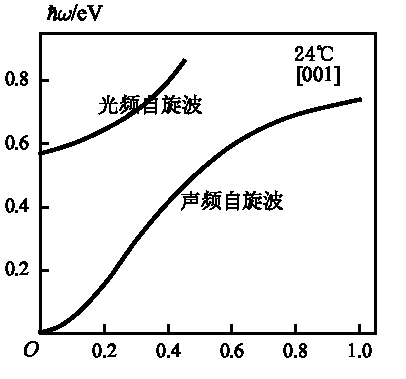
\includegraphics[width=8.5cm]{fig3-5.pdf}\\{\small 图 3.5\quad $\mathrm{Fe_3O_4}$ 中的自旋波}
\end{minipage}
\end{center}

低温比热容
\begin{equation}
  c_m=\nu Nk_{\mathrm{B}}\left(\frac{\left|S_a-S_b\right|}{4\left|J\right|S_aS_b}\right)^{3/2}
  \left(k_{\mathrm{B}}T\right)^{3/2}
\end{equation}
在计算时限于立方晶系，并且在低温区只需计算铁氧体自旋波中低频一支
$\omega_k^{(-)}$ 支的贡献，而略去 $\omega_k^{(+)}$ 支，其中的 $\alpha$ 与
$\nu$ 已在§4 中给出.
将以上结果与式(3.4.4)和式(3.4.15)相比较可见铁氧体的 $c_m$ 及 $M\left(T\right)$
也与铁磁体相似，大体上相当于
$JS\rightarrow\left|J\right|\,2S_aS_b/\left|S_a-S_b\right|$
.但是，由于铁氧体的 $J<0$
，其磁序特性又类似于反铁磁体，例如铁氧体中子格的自旋零点偏离为
\begin{equation}
  \Delta\mathcal{S}_a^{z}=\Delta\mathcal{S}_b^{z}
  =\frac{1}{2}\sum_k\left\{\left(1-c^2\gamma_k^2\right)^{-\frac{1}{2}}-1\right\}
\end{equation}
其中
\begin{equation}
  c=\frac{2\left(S_aS_b\right)^{\frac{1}{2}}}{\left(S_a+S_b\right)}
\end{equation}
当 $S_a=S_b$ 时，与反铁磁体的零点偏离公式(3.5.30)一致.

实际的铁氧体结构很复杂，例如，尖晶体型结构的铁锰氧体
$\left(\mathrm{MnFe_2O_4}\right)$ 含有 6 个 fcc
磁子晶格，应有多支自旋波谱，这将使计算变得困难.尽管如此，在长波限各支自旋波的频率与
$k^2$ 成正比的特征仍然不变.

\section{一维铁磁链中的孤波\textsuperscript{[12]}}

现在讨论磁振子之间的互作用对一维铁磁链中自旋运动的影响.设一维链中格点数为 $N$，当存在外磁场
$B$ 时一维链的各向异性海森伯模型设为
\begin{equation}
  H=-\mu B\sum_l\hat{S}_l^{z}
  -\frac{1}{2}J\sum_{l,\delta}\left(\hat{S}_l^{+}\hat{S}_{l+\delta}^{-}
  +\hat{S}_l^{-}\hat{S}_{l+\delta}^{+}\right)
  -J'\sum_{l,\delta}\hat{S}_l^{z}\hat{S}_{l+\delta}^{z}
\end{equation}
其中 $\mu\equiv g\mu_{\mathrm{B}}$，$J'>J>0$，晶格常数取为
1.为了讨论磁振子之间的相互作用，应计入非线性效应.利用近似展开式(3.3.29)，将自旋算符与场算符间的霍斯坦因－普里马可夫变换式(3.3.15)写成
\begin{equation}
  \left.\begin{aligned}
    \hat{S}_l^{z}&=S-a_l^{+}a_l\\
    \hat{S}_l^{+}&\approx\sqrt{2S}\left(1-\frac{1}{4S}a_l^{+}a_l\right)a_l\\
    \hat{S}_l^{-}&\approx\sqrt{2S}\,a_l^{+}\left(1-\frac{1}{4S}a_l^{+}a_l\right)
  \end{aligned}\right\}
\end{equation}
代入式(3.7.1)，求得准至场算符四次项的哈密顿量
\begin{equation}
\begin{aligned}
  H={}&-2J'S^2N-\mu BSN+\mu B\sum_l a_l^{+}a_l
  +S\sum_{l,\delta}\bigl\{J'\left(a_l^{+}a_l+a_{l+\delta}^{+}a_{l+\delta}\right)\\
  &-J\left(a_la_{l+\delta}^{+}+a_l^{+}a_{l+\delta}\right)\bigr\}
  -J'\sum_{l,\delta}a_l^{+}a_la_{l+\delta}^{+}a_{l+\delta}\\
  &+\frac{1}{4}J\sum_{l,\delta}\left(a_l^{+}a_{l+\delta}^{+}a_{l+\delta}a_{l+\delta}
  +a_{l+\delta}^{+}a_l^{+}a_la_l+a_l^{+}a_l^{+}a_la_{l+\delta}\right.\\
  &\qquad\qquad\left.+a_{l+\delta}^{+}a_{l+\delta}^{+}a_{l+\delta}a_l\right)
\end{aligned}
\end{equation}
算符 $a_l$ 的运动方程为
\begin{equation}
\begin{aligned}
  \mathrm{i}\hbar\frac{\partial a_l}{\partial t}&=\left(\mu B+4J'S\right)a_l
  -2JS\sum_\delta a_{l+\delta}
  -2J'\sum_\delta a_{l+\delta}^{+}a_{l+\delta}a_l\\
  &\quad+\frac{1}{2}J\sum_\delta\left(a_{l+\delta}^{+}a_{l+\delta}a_{l+\delta}
  +a_{l+\delta}^{+}a_la_l+2a_l^{+}a_la_{l+\delta}\right)
\end{aligned}
\end{equation}
这是一个非线性的算符方程.当 $B=0$
时，如果略去式(3.7.4)右边的非线性项并令 $J'=J$
，它立刻简化为式(3.3.32)，代表自旋波模式的运动方程.

上述非线性算符方程可利用相干态方法\textsuperscript{[13]}
变换为自旋运动的概率幅(probability amplitude)方程.
设系统 $H$ 的解由态 $|\Psi\rangle$ 描述，则 $l$
格点上自旋运动的概率幅可定义为
\begin{equation}
  \alpha_l\equiv\langle\Psi\mid a_l\mid\Psi\rangle
\end{equation}
$\alpha_l$
是复量，可以用 $\alpha_l$
标记各格点上自旋运动状态 $|\alpha_l\rangle$，并将系统的态用 $|\alpha_l\rangle$ 的直接乘积表示
\begin{equation}
  |\Psi\rangle=\prod_l|\alpha_l\rangle\equiv|\{\alpha_l\}\rangle
\end{equation}
根据式(3.7.5)和(3.7.6)，得到非厄密算符 $a_l$ 的本征方程
\begin{equation}
  a_l|\alpha_l\rangle=\alpha_l|\alpha_l\rangle
\end{equation}
这样确定的 $|\Psi\rangle$
称为相干态.应注意，相干态中 $|\alpha\rangle$
与§3 中确定磁振子数的状态 $|n\rangle$
不同，两者的关系可参考附录 F.
此外，在附录 F
中还证明了相干态是最小的不确定态，也可以说它是最经典的量子态，因此用相干态描述自旋的运动将是一种良好的近似.

将非线性算符方程式(3.7.4)作用于态 $|\{\alpha_l\}\rangle$
上，运用关系式(3.7.7)，容易求得概率幅方程
\begin{equation}
\begin{aligned}
  \mathrm{i}\hbar\frac{\partial\alpha_l}{\partial t}
  &=\left\{\mu B+4\left(J'-J\right)S\right\}\alpha_l
  +2JS\left(2\alpha_l-\alpha_{l+1}-\alpha_{l-1}\right)\\
  &\quad-2J'\left(\left|\alpha_{l+1}\right|^2+\left|\alpha_{l-1}\right|^2\right)\alpha_l\\
  &\quad+\frac{1}{2}J\sum_\delta\left(2\left|\alpha_l\right|^2
  +\left|\alpha_{l+\delta}\right|^2\right)\alpha_{l+\delta}
  +\frac{1}{2}J\alpha_l^2\sum_\delta\alpha_{l+\delta}^{*}
\end{aligned}
\end{equation}
当 $\alpha_l\left(t\right)$
在链中发生显著变化的空间尺度比晶格常数大得多时，可假定自旋运动的概率幅
$\alpha_l\left(t\right)$
是空间缓变量，并采用连续模型.为此，定义一个连续化的函数
$\alpha\left(x,t\right)$ 描述概率幅的时空变化
\begin{equation}
  \alpha\left(x,t\right)|_{x=l}\equiv\alpha_l\left(t\right)
\end{equation}
在连续模型近似下
\begin{equation}
  \alpha_{l\pm1}\left(t\right)-\alpha_l\left(t\right)=\pm\frac{\partial\alpha\left(x,t\right)}{\partial x}
  +\frac{1}{2}\frac{\partial^2\alpha\left(x,t\right)}{\partial x^2}+\cdots
\end{equation}
其中取晶格常数为 1.
相应的概率幅方程经上述连续化手续后，可近似写为下列非线性方程
\begin{equation}
\begin{aligned}
  \mathrm{i}\hbar\frac{\partial\alpha\left(x,t\right)}{\partial t}
  &+2JS\frac{\partial^2\alpha\left(x,t\right)}{\partial x^2}
  +4\left(J'-J\right)\left|\alpha\left(x,t\right)\right|^2\alpha\left(x,t\right)\\
  &=\left[\mu B+4\left(J'-J\right)S\right]\alpha\left(x,t\right)
\end{aligned}
\end{equation}
对上式作变换
\begin{equation*}
  \alpha\left(x,t\right)=\mathrm{e}^{-\mathrm{i}\lambda t}\phi\left(\xi,t\right)
\end{equation*}
\begin{equation}
  \xi\equiv\sqrt{\frac{\hbar}{2JS}}\,x
\end{equation}
若将参量 $\lambda$ 取为
\begin{equation}
  \hbar\lambda=\mu B+4\left(J'-J\right)S
\end{equation}
可消去式(3.7.11)右边的项，求得 $\phi\left(\xi,t\right)$ 的方程
\begin{equation*}
  \mathrm{i}\phi_t+\phi_{\xi\xi}+2Q\left|\phi\right|^2\phi=0
\end{equation*}
\begin{equation}
  Q\equiv\frac{2\left(J'-J\right)}{\hbar}>0
\end{equation}
式(3.7.14)是孤子问题中的非线性薛定谔方程(NLS)\textsuperscript{[14]}，它有标准解
\begin{equation}
  \phi\left(\xi,t\right)=A\exp\left[\mathrm{i}\,\frac{v_1}{2}\left(\xi-v_2t\right)\right]
  \mathrm{sech}\left[\sqrt{Q}\,A\left(\xi-v_2t\right)\right]
\end{equation}
其中 $A$ 为参量，$v_1$ 为积分常数，$v_2$
由上式代入非线性方程式(3.7.14)决定，当解满足方程时
\begin{equation}
  \frac{1}{2}\hbar v_1v_2=\hbar v_1^2-QA^2
\end{equation}
利用归一条件 $\int\left|\alpha\left(x,t\right)\right|^2\mathrm{d}x=1$ 可定出
$A=1/\sqrt{2L}$.相应的归一概率幅写成
\begin{equation}
  \alpha\left(x,t\right)=\frac{1}{\sqrt{2L}}
  \exp\left[\mathrm{i}\left(\gamma x-\omega t\right)\right]
  \mathrm{sech}\left[\frac{x-vt}{L}\right]
\end{equation}
其中
\begin{equation}
  L=\frac{2JS}{\left(J'-J\right)}\,,\qquad
  v=v_1\sqrt{\frac{2JS}{\hbar}}\,,\qquad
  \gamma=\frac{\hbar v}{4JS}
\end{equation}
\begin{equation}
  \hbar\omega\equiv E=\hbar\lambda+\frac{\hbar}{2}v_1v_2
  =\left[\mu B+4\left(J'-J\right)S+\frac{\hbar^2v^2}{8JS}
  -\frac{\left(J'-J\right)^2}{2JS}\right]
\end{equation}
解 $\alpha\left(x,t\right)$
代表相速为 $\left(\omega/\gamma\right)$
的振荡波，其包络是一个钟形峰，峰宽由 $L$
量度，包络中心以确定速度 $v$
在一维链中传播，传播过程中包络的形状不变，因此 $\alpha\left(x,t\right)$
振荡波的包络构成一个稳定的钟形孤波，称为包络孤子，$L$
代表包络孤子的尺寸.连续化近似要求孤子尺寸远远大于晶格常数，即必须
\begin{equation}
  L>\!>1
\end{equation}
这个条件意味着 $J'>J$，它与本节开始时的假定一致.$\hbar\omega$
代表孤波的量子.显然，它比线性自旋波理论中的磁振子能量要低
$\left(J'-J\right)^2/2JS$
量级，说明在一维铁磁链中由于非线性互作用所导致的孤波解是稳定解.当 $J'=J$ 时，
$L\rightarrow\infty$，这时由式(3.7.17)得到 $\alpha\left(x,t\right)=0$
，似乎表明对于各向同性的一维铁磁链不存在孤波解.但是实际情况并非如此，进一步的研究已经证明\textsuperscript{[15]}：如果将
$\hat{\boldsymbol{S}}_l^{\pm}$
的变换式(3.3.15)展开到更高阶项（包括 $S^0,S^{-1},S^{-2}$
项），即使是各向同性情况也可求得包络孤子解.

因此，我们可以说一维铁磁链中包络孤子解的存在是磁振子之间互作用所导致的.除包络孤子外，在一维磁体中还存在其它类型的孤子解，如扭型孤子解和脉冲状孤子解等.目前磁性孤子已经证实是低维系中自旋运动的一种模式，它代表系统的非线性元激发，20
世纪 80
年代以来在理论和实验研究方面都有较大进展\textsuperscript{[16]}.

\begin{canKao}
\begin{enumerate}[label={[\arabic*]}, leftmargin=2.2em, itemsep=0pt]
\item Heisenberg W. Phys Z, 1928, 49: 619
\item Dirac PAM. Proc Roy Soc, 1929, A123: 714
\item Anderson PW. Solid State Phys, 1963, 14: 99
\item Kittel C. Quantum Theory of Solids. New York: John Wiley \& Sond, Inc, 1963
\item Holstein T, Primakoff H. Phys Rev, 1940, 58: 1098
\item Dietrich OW {\it et al}. Phys Rev, 1976, B14: 4932
\item Bloch F. Z. Phys, 1930, 61: 206
\item Dyson F J. Phys Rev, 1956, 102: 1217, 1230
\item Bogoliubov N N. J Phys USSR, 1947, 11: 23
\item Anderson P W. Phys Rev, 1952, 86: 694
\item Jacobs LS. J. Appl Phys, 1961, 32: 615
\item Pushkarov D I {\it et al}. Phys Lett, 1977, 61A: 339
\item Glauber R J. Phys Rev, 1963, 131: 2766
\item Eilenberger G. Solitons. Berlin: Spinger-Verlag, 1981
\item Cordeiro C E {\it et al}. Phys Lett, 1978, 66A: 332
\item 蒲富恪，李伯臧.一维磁体中磁性孤子研究的进展.第五届全国磁学会议.1983
\end{enumerate}
\end{canKao}

% ============================================================
%  第四章 等离激元（§1–§11 + 参考文献）
%  底本：高等教育出版社《固体理论》第二版；原书印刷页 89–137
%  （PDF 页 = 印刷页 + 20）
%  公式编号：每节自 (4.N.1) 起自动编号，共 255 个编号
%  （其中 (4.9.27)、(4.9.28)、(4.9.30)、(4.11.30) 各分 a/b(/c) 两三式）
%
%  已修正的 OCR 错误：
%  1. §1 章首"集体振荡量子 ħωq"后 OCR 复制的 $\hbar\omega_q$ 已删（对照 p110）；
%     "如图4.1所示"中混入的 q 已删（p111）。
%  2. §2 (4.2.2)(4.2.5)(4.2.6)(4.2.9) 中被拆散的 v(q)、带撇求和号按 p113 修复；
%     (4.2.3) \hat{o}→δ；(4.2.8) \dot{C}→C^+；e²/r 傅里叶展开式原书无编号，
%     OCR 的空 \tag{} 已去掉。
%  3. §3 (4.3.3) "4πe²i/m"、(4.3.5) q·q′/q′² 按 p115 修复；(4.3.7) Σi→Σj。
%  4. §4 (4.4.2) φ→ρ̇；(4.4.8) C^-→C；(4.4.9) 整块按 p117 重排；
%     (4.4.10) \widehat{θ}→δ。
%  5. §5 (4.5.13)(4.5.15) 下标 ι、误入的 \hbar 杂符按 p119–120 修复。
%  6. §6 (4.6.6) 整式按 p122 重排；∈/E/e 等介电函数记号统一为 ε；
%     (4.6.9) (−ε)→(−e)；(4.6.22) \mathfrak{E}→δ；(4.6.24) 句尾杂符已删；
%     (4.6.14) 按原书（p122 底—p123 顶跨页一式）补回首行 ε=Ve/V。
%  7. §6 林哈德 ε1、ε2 显式式（(4.6.25)(4.6.26)）OCR 并作一块且严重乱码，
%     已按 p124 原书页面拆成两式重排。
%  8. §7 (4.7.4) 的编号 OCR 掉到正文，已归还该式（p126）。
%  9. §8 (4.8.7) q0r→qcr；\hat{δ}→δ。
% 10. §9 (4.9.5) 编号 OCR 缺失，按正文引用证实该式即 (4.9.5)（p134）；
%     (4.9.7) 相邻两块 $$ 按原书合并为一式（p134–135）；
%     \hat{δ}/\widehat{⊗}/\mathfrak{d}→δ；(4.9.40) φ/ψ 混用统一为 ψ；
%     (4.9.60) 按原书（p142）补为三行等式（OCR 只存首行）；
%     (4.9.71) 补回 "=" 续行；(4.9.73)(4.9.75)(4.9.77)(4.9.78) 的残缺
%     tag（{73}/(4.9.75)/{.77}/{9.78}）按 p144–145 恢复；
%     (4.9.27)(4.9.28)(4.9.30) 的 a/b 分编号按 p137–138 恢复。
% 11. §10 (4.10.10) 首行分母按 (4.10.4) 应为 2r0（原书印作 2rs，已改并注）。
% 12. §11 (4.11.2)(4.11.4) \hat{⊗}→δ、误入的 \hbar 已删（p149–150）；
%     \tag{1.5}→(4.11.5)；(4.11.30a) 按 p154 重排；T_k→Γ_k；θ_k→g_k；
%     "利费密黄金规则"→"利用费密黄金规则"；p150 脚注①已补录；
%     章首段"[在量子多体理论中称为自能……详见附录C]也是复量"按 p148 恢复。
% 13. 全章：全角句号"．/。"→ ASCII "."；OCR 间隔符 ~ 删除；"5~30 eV"→"5～30 eV"；
%     "F格"→"严格"；"这个积分长在波限"→"这个积分在长波限"（原书倒字）；
%     附录A一D→附录A—D；Kohnanomalies→Kohn anomalies；
%     "求动能部分 对ij^m格基态的平均"→"求动能部分……对严格基态的平均"（p139）。
%  原书排印错误（照页面修正，均已在正文按原样改正）：
%  A. p130 "当 qcr→2 时 Si(qcr)→π/2"→ qcr→∞（物理极限）；
%  B. p130 "库仑势中自然只剩下短波成分 (q<qc)"→ (q>qc)（与上下文物理矛盾）；
%  C. p138 (4.9.30a)(4.9.30b) 的 lim 下标 q→0→ q→∞（上下文为大 q 渐近）；
%  D. p117 (4.4.11) 左端 ρ_{kp}^+→ρ_{kq}^+（按式 (4.4.10) 上下文）；
%  E. p132 (4.8.12) 右端 Z/8π³ 与 4πZe² 重复计 Z，按 (4.8.11) 傅里叶逆
%     改为 1/8π³。
%  遗留问题：
%  · 文献[7] "Solid State Phys, 1995" 系原书如此（史实为 1955），照录未改；
%  · 图4.2 无裁剪图，占位图待重绘代理按原书 p112 绘制；原书图注仅"图 4.2"；
%  · (4.4.11) 原书左端下标 kp/q 印刷难辨，按物理取 kq。
% ============================================================
\chapter{等离激元}

本章讨论在宽能带金属中，当价电子之间存在库仑互作用时的元激发特征.由于库仑互作用的长程性以及价电子易动的巡游性，将导致电子系统既存在集体激发（等离激元），又出现个别激发（准电子），在理论上属于不能严格对角化的多体系统，必须采用近似方法.为了将所研究的体系变为纯粹的电子-电子相互作用系统，在本章中暂时略去晶格周期场和晶格振动（声子）对电子的影响，采用一个简化的金属模型（§2），并介绍一种在高密度条件下可以求解经典及量子运动方程的合理近似——无规相近似（见§3、§4）.在此基础上，我们将采用动态介电函数方法研究相互作用电子系统对含时外扰动的线性响应（§5），并求出无规相近似介电函数（§6），这种新方法的优点是，可以统一求出系统的个别与集体激发（§7），屏蔽效应（§8），并解决金属基态能计算的发散困难.最后，在§11中将证明相互作用电子系统中仍然存在费密面.采用动态介电函数方法的另一优点是，可以通过热力学格林函数直接推广到有限温度情形，因此在学习本章时应同时阅读附录A—D中有关的格林函数介绍.

\section{等离激元和准电子}

先介绍电子-电子互作用系统元激发的物理图像.以金属中的电子为例，价电子在离子的正电抵消背景上运动，系统在宏观尺度上保持着电中性.由于价电子易动，而且电子间有相互作用，因此系统在微观尺度上必然存在着电子密度的起伏.鉴于电子间相互作用是库仑势，具有长程作用的特征，所以哪怕是局域的密度起伏也将在整个系统中产生电子运动的关联，这是一种集体效应.人们常采用系统中电子密度的傅里叶分量 $\rho_{q}$ 作为集体坐标来描述这种关联.与晶格振动问题中的集体坐标相类似，在这里 $\rho_{q}$ 将以波动的形式出现，它是系统中电子密度起伏相对于正电背景的振荡，称为等离子区集体振荡.波矢为 $\boldsymbol{q}$ 频率为 $\omega_{q}$ 的等离子区集体振荡量子 $\hbar\omega_{q}$，在固体物理中，叫做等离激元（plasmons）.等离激元的频率在长波长时容易求出，此时可设每个电子相对于正离子背景的移动均为 $x$，电子移动后所产生的电场
\begin{equation*}
  \mathcal{E}=4\pi Nex
\end{equation*}
$N$ 是单位体积中的价电子数，于是作用于每个电子上的恢复力为 $-e\mathcal{E}$，电子运动满足方程
\begin{equation*}
  m\ddot{x}=-4\pi Ne^{2}x
\end{equation*}
显然，每一个电子均以相同的频率
\begin{equation}
  \omega_{\mathrm{p}}^{2}=\frac{4\pi Ne^{2}}{m}
\end{equation}
振荡，$\hbar\omega_{\mathrm{p}}$ 一般为 5～30 eV.在本章中我们将利用二次量子化工具较严格的确定每个波矢 $\boldsymbol{q}$ 对应的等离激元能量 $\hbar\omega_{q}$，求出其色散关系.式(4.1.1)仅仅是 $q=0$ 时的频率.

除集体激发以外，金属中还存在电子的个别激发.讨论金属中电子的个别行为时，必须考虑费密面的存在，这时从 $\boldsymbol{k}$ 空间分析问题图像更为清楚.系统的“真空”（即基态）可近似描述为在费密球 $k_{\mathrm{F}}$ 内的所有状态均被电子占据，而球外则全空着.相对于这个“真空”的个别激发是从费密球内 $\boldsymbol{k}$ 态上拿出一个电子放到球外 $\boldsymbol{k}+\boldsymbol{q}$ 空状态上去，于是在金属的“真空”上产生了一个 $\boldsymbol{k}+\boldsymbol{q}$ 电子和一个 $\boldsymbol{k}$ 空穴，这种电子和空穴对的个别激发能量记作
\begin{equation}
  \hbar\omega_{kq}=\frac{\hbar^{2}(\boldsymbol{k}+\boldsymbol{q})^{2}}{2m}
  -\frac{\hbar^{2}k^{2}}{2m}
  =\frac{\hbar^{2}}{2m}\left(q^{2}+2\boldsymbol{k}\cdot\boldsymbol{q}\right)
\end{equation}
对于确定的 $\boldsymbol{q}$，存在着一个受泡利原理限制的许可区域，如图4.1所示.

\begin{center}
\begin{minipage}{8.5cm}
\centering
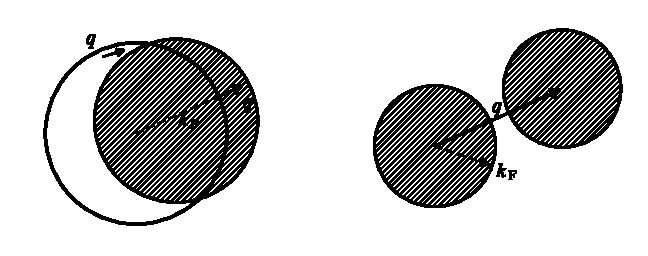
\includegraphics[width=8.5cm]{fig4-1.pdf}\\[0.3em]
{\small (a) $q<2k_{\mathrm{F}}$\qquad\qquad (b) $q>2k_{\mathrm{F}}$}\\[0.2em]
{\small 图 4.1}
\end{minipage}
\end{center}

（i）$q<2k_{\mathrm{F}}$：此时并非球内每个电子都可激发到球外，只有图4.1(a)中两个弯月形才是许可的区域，其中内层的阴影区是空穴激发区，外层的阴影区代表电子激发区.由图还可以定出激发能 $\hbar\omega_{kq}$ 的界限为
\begin{equation}
  \hbar\omega_{kq}^{\max}=\frac{\hbar^{2}}{2m}\left(q^{2}+2k_{\mathrm{F}}q\right);\quad
  \hbar\omega_{kq}^{\min}=0
\end{equation}
（ii）$q>2k_{\mathrm{F}}$：费密球内全为空穴激发区，另一个原点在 $\boldsymbol{q}$ 的球内［见图4.1(b)］是电子激发区，对应 $\hbar\omega_{kq}$ 的界限为
\begin{equation}
  \hbar\omega_{kq}^{\max}=\frac{\hbar^{2}}{2m}\left(q^{2}+2k_{\mathrm{F}}q\right);\quad
  \hbar\omega_{kq}^{\min}=\frac{\hbar^{2}}{2m}\left(q^{2}-2k_{\mathrm{F}}q\right)
\end{equation}
图4.2中注明的对激发区，是按照公式(4.1.3)和(4.1.4)作出的，在同一图中也绘出了等离激元的色散曲线 $\omega_{q}$.在§5中将证明等离激元的长波色散关系为
\begin{equation}
  \omega_{q}=\omega_{\mathrm{p}}+\frac{3v_{\mathrm{F}}^{2}q^{2}}{10\omega_{\mathrm{p}}}
\end{equation}
其中 $v_{\mathrm{F}}$ 为费密速度，$v_{\mathrm{F}}=\hbar k_{\mathrm{F}}/m$.

\begin{center}
\begin{minipage}{5.5cm}
\centering
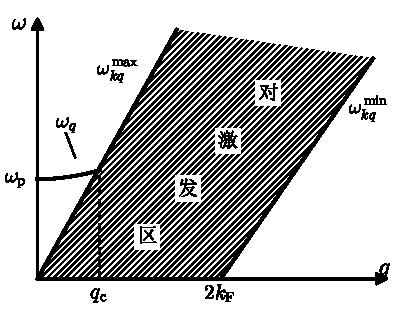
\includegraphics[width=5.5cm]{fig4-2.pdf}\\{\small 图 4.2}
\end{minipage}
\end{center}

由图4.2可以看出，存在着集体振荡与电子-空穴时个别激发区的交点 $q_{c}$.当 $q<q_{c}$ 时，等离激元能量 $\hbar\omega_{q}$ 大于电子-空穴对个别激发的最大能量 $\hbar\omega_{kq}^{\max}$，集体振荡既不可能被个别对所激发，也不可能衰减为个别的电子-空穴对.但是，当 $q>q_{c}$ 时由于 $\hbar\omega_{kq}^{\max}>\hbar\omega_{q}$，将出现振荡的衰减.在§5中我们将分析电子系统的介电函数，并证明 $q>q_{c}$ 时等离子区集体振荡是不稳定的.因此，仅仅在长波范围 $0<q<q_{c}$ 之内，才有集体激发（等离激元）存在，而当 $q>q_{c}$ 时，只有个别对激发，$q_{c}$ 可认为是划分金属电子系统个别激发与集体激发的特性参量.在相互作用电子系统中，长波范围（小 $q$）内主要是集体振荡，短波（大 $q$）时为普通的电子-空穴对激发.

电子间相互作用对于金属中个别电子的性能也有影响，其中特别重要的是屏蔽效应，库仑作用使得每个电子周围形成了正电荷的屏蔽壳层，它跟随着激发它的电子一起运动，从而改变电子间的相互作用势和电子的有效质量.人们把（电子$+$屏蔽电荷）的整体称为准电子（quasi-electrons）.准电子间互作用不再是库仑势，而是汤川型屏蔽库仑势 $\dfrac{e^{2}}{r}\mathrm{e}^{-\lambda r}$，$\lambda$ 与 $q_{c}$ 同量级（见§8）.因此，准电子间的有效互作用近似为 $\dfrac{e^{2}}{r}\mathrm{e}^{-q_{c}r}$，它与 $\displaystyle\sum_{q>q_{c}}\frac{4\pi e^{2}}{q^{2}}\mathrm{e}^{\mathrm{i}\boldsymbol{q}\cdot\boldsymbol{r}}$ 大致相同，说明互作用来自库仑势 $\dfrac{e^{2}}{r}$ 展开的短波部分.显然，库仑势展开的长波部分被扣除了，这是因为库仑作用的长程部分已用于电子系统的集体振荡.

\section{互作用电子系统的哈密顿量}

当讨论金属中电子的元激发特征时，能带效应并不重要.可以把排成晶格的正离子近似当作是均匀抹平了的连续正电荷分布，像凝胶（jellium）一样.公有化电子则在此正电荷背景上运动，整个系统保持电中性.这种简化的金属电子模型称为凝胶模型.

电子体系的哈密顿量为
\begin{equation}
  H=-\sum_{i=1}^{N}\frac{\hbar^{2}\nabla_{i}^{2}}{2m}
  +\frac{1}{2}\mathop{{\sum}'}\limits_{i,j}\frac{e^{2}}{|\boldsymbol{r}_{i}-\boldsymbol{r}_{j}|}
  +H_{+}
\end{equation}
其中 $H_{+}$ 是均匀分布正电荷背景的贡献项，包括正电背景的自作用能以及它与电子的互作用能.为简单起见，设公有化电子数为 $N$，并取单位体积样品 $V=1$，将 $e^{2}/r$ 作傅里叶展开
\begin{equation*}
  \frac{e^{2}}{r}=\sum_{\boldsymbol{q}}v(\boldsymbol{q})\mathrm{e}^{\mathrm{i}\boldsymbol{q}\cdot\boldsymbol{r}},
  \quad v(\boldsymbol{q})=\frac{4\pi e^{2}}{q^{2}}
\end{equation*}
则
\begin{equation}
  H=-\sum_{i=1}^{N}\frac{\hbar^{2}\nabla_{i}^{2}}{2m}
  +\frac{1}{2}\sum_{\boldsymbol{q}}\mathop{{\sum}'}\limits_{i,j}
  v(\boldsymbol{q})\mathrm{e}^{\mathrm{i}\boldsymbol{q}\cdot(\boldsymbol{r}_{i}-\boldsymbol{r}_{j})}
  +H_{+}
\end{equation}
根据§1中讨论，用电子密度的傅里叶分量表示 $H$，由于电子的密度
\begin{equation}
  \rho(\boldsymbol{r})=\sum_{j}\delta(\boldsymbol{r}-\boldsymbol{r}_{j})
  =\sum_{\boldsymbol{q}}\sum_{j}\mathrm{e}^{\mathrm{i}\boldsymbol{q}\cdot(\boldsymbol{r}-\boldsymbol{r}_{j})}
  \equiv\sum_{\boldsymbol{q}}\rho_{q}\mathrm{e}^{\mathrm{i}\boldsymbol{q}\cdot\boldsymbol{r}}
\end{equation}
因此密度 $\rho(\boldsymbol{r})$ 的傅里叶分量为
\begin{equation}
  \rho_{q}=\sum_{j}\mathrm{e}^{-\mathrm{i}\boldsymbol{q}\cdot\boldsymbol{r}_{j}},\quad
  \rho_{q}^{+}=\sum_{j}\mathrm{e}^{\mathrm{i}\boldsymbol{q}\cdot\boldsymbol{r}_{j}}=\rho_{-q}
\end{equation}
代入式(4.2.2)得到
\begin{equation}
  H=-\sum_{i=1}^{N}\frac{\hbar^{2}\nabla_{i}^{2}}{2m}
  +\frac{1}{2}\sum_{q}v(q)\left(\rho_{q}^{+}\rho_{q}-N\right)+H_{+}
\end{equation}
其中 $-\dfrac{1}{2}v(q)N$ 为扣除的 $i=j$ 项，第二个求和项中的 $q=0$ 部分代表均匀分布的电子自作用能，在凝胶模型中恰好与 $H_{+}$ 相抵消.因此，在哈密顿量中可略去 $H_{+}$，只取 $q\neq 0$ 项，这时 $\rho_{q}$ 代表密度起伏.
\begin{equation}
  H=-\sum_{i=1}^{N}\frac{\hbar^{2}\nabla_{i}^{2}}{2m}
  +\frac{1}{2}\mathop{{\sum}'}\limits_{q}v(q)\left(\rho_{q}^{+}\rho_{q}-N\right)
\end{equation}
这就是凝胶模型中电子系统的哈密顿量.

在二次量子化表象中，$\rho_{q}$ 与 $\rho_{q}^{+}$ 对应于密度起伏算符，有关系式
\begin{equation}
\begin{aligned}
  \rho(\boldsymbol{r},t)
  &=\int\varPsi^{+}(\boldsymbol{r}',t)\delta(\boldsymbol{r}-\boldsymbol{r}')
  \varPsi(\boldsymbol{r}',t)\,\mathrm{d}\boldsymbol{r}'\\
  &=\varPsi^{+}(\boldsymbol{r},t)\varPsi(\boldsymbol{r},t)\\
  &=\sum_{k,k'}C_{k}^{+}C_{k'}\mathrm{e}^{-\mathrm{i}(\boldsymbol{k}-\boldsymbol{k}')\cdot\boldsymbol{r}}\\
  &=\sum_{k,q}C_{k}^{+}C_{k+q}\mathrm{e}^{\mathrm{i}\boldsymbol{q}\cdot\boldsymbol{r}}
  \qquad\left(\boldsymbol{q}\equiv\boldsymbol{k}'-\boldsymbol{k}\right)
\end{aligned}
\end{equation}
由此求得 $\rho_{q}$、$\rho_{q}^{+}$ 与产生及消灭算符 $C_{k}^{+}$、$C_{k'}$ 的关系为：
\begin{equation}
  \left.\begin{aligned}
  \rho_{q}&=\sum_{k}C_{k}^{+}C_{k+q}=\sum_{k}C_{k-q}^{+}C_{k}\\
  \rho_{q}^{+}&=\sum_{k}C_{k+q}^{+}C_{k}=\rho_{-q}
  \end{aligned}\right\}
\end{equation}
则哈密顿量
\begin{equation}
  H=\sum_{k}E_{k}C_{k}^{+}C_{k}
  +\frac{1}{2}\mathop{{\sum}'}\limits_{q}v(q)\left(\rho_{q}^{+}\rho_{q}-N\right)
\end{equation}
其中 $E_{k}=\hbar^{2}k^{2}/2m$，$C_{k}$ 与 $C_{k}^{+}$ 满足费密子反对易式
\begin{equation}
  \left.\begin{aligned}
  [\,C_{k},C_{k'}^{+}\,]_{+}&=C_{k}C_{k'}^{+}+C_{k'}^{+}C_{k}=\delta_{kk'}\\
  [\,C_{k},C_{k'}\,]_{+}&=[\,C_{k}^{+},C_{k'}^{+}\,]_{+}=0
  \end{aligned}\right\}
\end{equation}
为简单起见，在以上表示式中没有明确写出电子的自旋标记 $\sigma$，实际上
\begin{equation}
  \rho_{q}=\sum_{k,\sigma}C_{k-q,\sigma}^{+}C_{k\sigma},\quad
  \rho_{q}^{+}=\sum_{k,\sigma}C_{k+q,\sigma}^{+}C_{k,\sigma}
\end{equation}
而总哈密顿量为
\begin{equation}
\begin{aligned}
  H&=\sum_{k,\sigma}E_{k}C_{k\sigma}^{+}C_{k\sigma}
  +\frac{1}{2}\mathop{{\sum}'}\limits_{q}v(q)\left(\rho_{q}^{+}\rho_{q}-N\right)\\
  &=\sum_{k,\sigma}E_{k}C_{k\sigma}^{+}C_{k\sigma}
  +\frac{1}{2}\mathop{{\sum}'}\limits_{q}\sum_{k,k'}\sum_{\sigma,\sigma'}
  v(q)C_{k+q,\sigma}^{+}C_{k'-q,\sigma'}^{+}C_{k'\sigma'}C_{k\sigma}
\end{aligned}
\end{equation}
与通常的标准形式一样.

\section{电子集体振荡的经典理论}

讨论经典情况的目的，是为了介绍求解电子等离子集体振荡的合理近似方法.

式(4.2.3)对时间求导，得
\begin{equation}
  \dot{\rho}_{q}=-\mathrm{i}\sum_{j}\boldsymbol{q}\cdot\boldsymbol{v}_{j}\,
  \mathrm{e}^{-\mathrm{i}\boldsymbol{q}\cdot\boldsymbol{r}_{j}}
\end{equation}
这里 $\boldsymbol{v}_{j}=\dot{\boldsymbol{r}}_{j}$ 是第 $j$ 个电子的速度，再求导，得方程
\begin{equation}
  \ddot{\rho}_{q}=-\sum_{j}\left\{\left(\boldsymbol{q}\cdot\boldsymbol{v}_{j}\right)^{2}
  +\mathrm{i}\boldsymbol{q}\cdot\dot{\boldsymbol{v}}_{j}\right\}
  \mathrm{e}^{-\mathrm{i}\boldsymbol{q}\cdot\boldsymbol{r}_{j}}
\end{equation}
$\dot{\boldsymbol{v}}_{j}$ 由经典力学方程决定
\begin{equation}
  \dot{\boldsymbol{v}}_{j}=-\frac{1}{m}\nabla_{j}
  \left\{\frac{1}{2}\mathop{{\sum}'}\limits_{q'}v(q')
  \left(\rho_{q'}^{+}\rho_{q'}-N\right)\right\}
  =-\frac{4\pi e^{2}\mathrm{i}}{m}\mathop{{\sum}'}\limits_{q'}
  \frac{\boldsymbol{q}'}{q'^{2}}\rho_{q'}\mathrm{e}^{\mathrm{i}\boldsymbol{q}'\cdot\boldsymbol{r}_{j}}
\end{equation}
其中 $\mathop{{\sum}'}\limits_{q'}$ 表示限制 $q'\neq 0$，是由于考虑了电子体系中均匀正电背景的影响.将 $\dot{\boldsymbol{v}}_{i}$ 代入 $\ddot{\rho}_{q}$ 方程，求得电子密度的傅里叶分量 $\rho_{q}$ 满足下列非线性的运动方程：
\begin{equation}
  \ddot{\rho}_{q}=-\sum_{j}\left(\boldsymbol{q}\cdot\boldsymbol{v}_{j}\right)^{2}
  \mathrm{e}^{-\mathrm{i}\boldsymbol{q}\cdot\boldsymbol{r}_{j}}
  -\left(\frac{4\pi e^{2}}{m}\right)\mathop{{\sum}'}\limits_{q'}
  \frac{\boldsymbol{q}\cdot\boldsymbol{q}'}{q'^{2}}\rho_{q'}\rho_{q-q'}
\end{equation}
上式中右边第二项又可分成 $\boldsymbol{q}'=\boldsymbol{q}$ 和 $\boldsymbol{q}'\neq\boldsymbol{q}$ 两部分：
\begin{equation}
  -\left(\frac{4\pi e^{2}}{m}\right)
  \left\{N\rho_{q}+\mathop{{\sum}'}\limits_{q'(q'\neq q)}
  \frac{\boldsymbol{q}\cdot\boldsymbol{q}'}{q'^{2}}\rho_{q'}\rho_{q-q'}\right\}
\end{equation}
假如略去 $\boldsymbol{q}'\neq\boldsymbol{q}$ 项，只保留 $\boldsymbol{q}'=\boldsymbol{q}$ 项，则可将式(4.3.4)线性化为
\begin{equation}
  \ddot{\rho}_{q}=-\sum_{j}\left\{\frac{4\pi Ne^{2}}{m}
  +\left(\boldsymbol{q}\cdot\boldsymbol{v}_{j}\right)^{2}\right\}
  \mathrm{e}^{-\mathrm{i}\boldsymbol{q}\cdot\boldsymbol{r}_{j}}
\end{equation}
或
\begin{equation}
  \ddot{\rho}_{q}+\omega_{\mathrm{p}}^{2}\rho_{q}
  =-\sum_{j}\left(\boldsymbol{q}\cdot\boldsymbol{v}_{j}\right)^{2}
  \mathrm{e}^{-\mathrm{i}\boldsymbol{q}\cdot\boldsymbol{r}_{j}}
\end{equation}
当 $\boldsymbol{q}\to 0$ 时，可略去 $\left(\boldsymbol{q}\cdot\boldsymbol{v}_{j}\right)^{2}$ 项，求得 $\rho_{q}$ 的简谐振动方程
\begin{equation}
  \ddot{\rho}_{q}+\omega_{\mathrm{p}}^{2}\rho_{q}=0\quad(q\to 0)
\end{equation}
其中 $\omega_{\mathrm{p}}^{2}=\dfrac{4\pi Ne^{2}}{m}$ 是在长波限的等离子振荡频率，色散关系也可由方程(4.3.7)求出.

显然，在以上求解过程中主要的近似为，在式(4.3.5)中略去两个不同密度起伏模 $\rho_{q'}$ 与 $\rho_{q-q'}$ 之间的耦合项，其理由如下：由于 $\rho_{q}=\displaystyle\sum_{j}\mathrm{e}^{-\mathrm{i}\boldsymbol{q}\cdot\boldsymbol{r}_{j}}$ 是指数项之和，而这些指数的相位因子又由 $\boldsymbol{r}_{j}$ 决定，对于高密度电子系统，电子的位置在空间的分布是杂乱无规的，这时 $\rho_{q}\ (q\neq 0)$ 代表相位无规变化的指数项之和，对于平移不变的系统其平均值为零，所以两个密度起伏的乘积项对于运动方程(4.3.4)仅仅是微小的修正，作为一级近似可略去，这样的近似称为无规相近似（RPA）.这里无规相的含义正在于 $\rho_{q}$ 是无规相位的指数相加，而 $\rho_{0}=N$ 是各项的相干叠加，两者在高密度条件下相差很大.所以，式(4.3.5)中 $\rho_{q'}\rho_{q-q'}$ 相对于 $N\rho_{q}$ 是小量，略去它是合理的.

\section{量子运动方程的无规相近似}

我们将从算符的运动方程出发，求解互作用电子体系的近似本征值.定义电子-空穴对的激发算符
\begin{equation}
  \rho_{kq}^{+}\equiv C_{k+q}^{+}C_{k}
\end{equation}
$\rho_{kq}^{+}$ 作用于系统的“真空”，相当在费密球内 $\boldsymbol{k}$ 态上产生一个空穴，在球外 $\boldsymbol{k}+\boldsymbol{q}$ 态上产生一个电子，代表金属中的个别激发.在互作用电子系统中这些个别激发是彼此耦合在一起的，算符 $\rho_{kq}$ 及 $\rho_{kq}^{+}$ 的海森伯运动方程为
\begin{equation}
  -\mathrm{i}\hbar\dot{\rho}_{kq}=[H,\rho_{kq}];\quad
  -\mathrm{i}\hbar\dot{\rho}_{kq}^{+}=[H,\rho_{kq}^{+}]
\end{equation}
根据式(4.2.8)密度起伏 $\rho_{q}$，$\rho_{q}^{+}$ 是总动量为 $\hbar\boldsymbol{q}$ 的所有电子-空穴对运动的简单叠加
\begin{equation}
  \rho_{q}^{+}=\sum_{k}\rho_{kq}^{+}
\end{equation}
我们只要能解出电子-空穴对的运动方程(4.4.2)，则电子体系的元激发谱就求得了.

$\rho_{kq}^{+}$ 的本征方程为
\begin{equation}
  \left[H,\rho_{kq}^{+}\right]=\hbar\omega\rho_{kq}^{+}
\end{equation}
将上式代入方程(4.4.2)，得到 $-\mathrm{i}\hbar\dot{\rho}_{kq}^{+}=\hbar\omega\rho_{kq}^{+}$，说明 $\hbar\omega$ 代表能量本征值，而式(4.4.4)即类似于式(3.6.7)的运动方程的对角化条件.

式(4.4.2)或(4.4.4)是电子-空穴对激发的耦合方程.假如不存在相互作用，即 $\boldsymbol{v}(\boldsymbol{q})=0$，则 $H=\displaystyle\sum_{k}E_{k}C_{k}^{+}C_{k}\equiv H_{0}$ 代表独立电子系统，这时容易求得
\begin{equation}
  \left[H_{0},\rho_{kq}^{+}\right]
  =\left\{\frac{\hbar^{2}}{2m}(\boldsymbol{k}+\boldsymbol{q})^{2}
  -\frac{\hbar^{2}}{2m}k^{2}\right\}\rho_{kq}^{+}
  =\hbar\omega_{kq}\rho_{kq}^{+}
\end{equation}
这里 $\hbar\omega_{kq}$ 正如式(4.1.2)所定义，是不计相互作用时电子-空穴对的激发能量，代表电子-空穴的自由传播.

对于互作用电子体系 $\boldsymbol{v}(\boldsymbol{q})\neq 0$，上述对易式较复杂：
\begin{equation}
  \left[H,\rho_{kq}^{+}\right]=\hbar\omega_{kq}\rho_{kq}^{+}
  +\frac{1}{2}\mathop{{\sum}'}\limits_{q'}v(q')
  \big\{\left[\,\rho_{q'}^{+},\rho_{kq}^{+}\,\right]\rho_{q'}
  +\rho_{q'}^{+}\left[\,\rho_{q'},\rho_{kq}^{+}\,\right]\big\}
\end{equation}
由于 $\boldsymbol{v}(\boldsymbol{q})=\boldsymbol{v}(-\boldsymbol{q})$，$\rho_{q}^{+}=\rho_{-q}$，上式可改写为
\begin{equation}
  \left[H,\rho_{kq}^{+}\right]=\hbar\omega_{kq}\rho_{kq}^{+}
  +\frac{1}{2}\mathop{{\sum}'}\limits_{q'}v(q')
  \big\{\left[\,\rho_{q'},\rho_{kq}^{+}\,\right]\rho_{q'}^{+}
  +\rho_{q'}^{+}\left[\,\rho_{q'},\rho_{kq}^{+}\,\right]\big\}
\end{equation}
利用 $\left[A,BC\right]=\left[A,B\right]_{+}C-B\left[A,C\right]_{+}$，算出对易式
\begin{equation}
\begin{aligned}
  \left[\rho_{q'},\rho_{kq}^{+}\right]
  &=\Big[\sum_{k'}C_{k'-q'}^{+}C_{k'},C_{k+q}^{+}C_{k}\Big]\\
  &=C_{k+q-q'}^{+}C_{k}-C_{k+q}^{+}C_{k+q'}
\end{aligned}
\end{equation}
代入式(4.4.7)，并分出 $\boldsymbol{q}'=\boldsymbol{q}$ 与 $\boldsymbol{q}'\neq\boldsymbol{q}$ 项，整理后写成
\begin{equation}
\begin{aligned}
  \left[H,\rho_{kq}^{+}\right]={}&\hbar\omega_{kq}\rho_{kq}^{+}
  +\frac{1}{2}v(q)\big\{\big(C_{k}^{+}C_{k}-C_{k+q}^{+}C_{k+q}\big)\sum_{k'}\rho_{k'q}^{+}\\
  &+\sum_{k'}\rho_{k'q}^{+}\big(C_{k}^{+}C_{k}-C_{k+q}^{+}C_{k+q}\big)\big\}\\
  &+\frac{1}{2}\mathop{{\sum}'}\limits_{q'(q'\neq q)}v(q')
  \big\{\big(C_{k+q-q'}^{+}C_{k}-C_{k+q}^{+}C_{k+q'}\big)\rho_{q'}^{+}\\
  &\quad+\rho_{q'}^{+}\big(C_{k+q-q'}^{+}C_{k}-C_{k+q}^{+}C_{k+q'}\big)\big\}
\end{aligned}
\end{equation}
式(4.4.9)中右边第一项代表自由运动，第二项是具有相同 $\boldsymbol{q}$ 的所有电子-空穴对间的耦合，最后的求和项为不同 $\boldsymbol{q}$ 的电子-空穴对之间的相互作用，它表明一个总动量 $\hbar\boldsymbol{q}$ 的对将激发另一组 $\hbar\boldsymbol{q}'\,(\boldsymbol{q}'\neq\boldsymbol{q})$ 的电子-空穴对.若将第二项称为同“类”对间耦合，则第三项相当于异“类”$(\boldsymbol{q}'\neq\boldsymbol{q})$ 对之间的彼此激发，它们都属于 $\rho_{kq}^{+}$ 本征方程中的非线性部分，为了使算符方程(4.4.4)易于求解，我们将用下列线性化手续：

将式(4.4.8)中算符近似用其对“真空”态的平均值代替
\begin{equation}
\begin{aligned}
  \left[\rho_{q'},\rho_{kq}^{+}\right]
  &=\big(\langle C_{k+q-q'}^{+}C_{k}\rangle_{0}
  -\langle C_{k+q}^{+}C_{k+q'}\rangle_{0}\big)\\
  &=\big(\langle C_{k}^{+}C_{k}\rangle_{0}
  -\langle C_{k+q}^{+}C_{k+q}\rangle_{0}\big)\delta_{qq'}\\
  &=2\left(n_{k}-n_{k+q}\right)\delta_{qq'}
\end{aligned}
\end{equation}
这里由于平移对称性要求动量守恒.因此，只有同类对 $\boldsymbol{q}'=\boldsymbol{q}$ 项有贡献，而异“类”对间的激发自然被消去了，说明后者仅代表更高阶的互作用.这样式(4.4.9)线性化为
\begin{equation}
  \left[H,\rho_{kq}^{+}\right]=\hbar\omega_{kq}\rho_{kq}^{+}
  +2v(q)\left(n_{k}-n_{k+q}\right)\rho_{q}^{+}
\end{equation}
代入式(4.4.4)得到线性化的本征方程
\begin{equation}
  \hbar\left(\omega-\omega_{kq}\right)\rho_{kq}^{+}
  =2v(q)\left(n_{k}-n_{k+q}\right)\rho_{q}^{+}
\end{equation}
上式对 $k$ 求和，再利用式(4.4.3)消去 $\rho_{q}^{+}$，得到频率方程
\begin{equation}
  v(q)\sum_{k}\frac{2\left(n_{k}-n_{k+q}\right)}
  {\hbar\left(\omega-\omega_{kq}\right)}=1
\end{equation}
式中 $2n_{k}$ 是对真空态的平均
\begin{equation}
  \langle C_{k}^{+}C_{k}\rangle_{0}\equiv 2n_{k}=2\theta\left(k_{\mathrm{F}}-k\right)
\end{equation}
其中 $\theta(x)$ 为阶跃函数，真空态指的是自由电子的费密球分布状态，因子2来源于 $k$ 态上自旋简并，因为 $\langle C_{k}^{+}C_{k}\rangle_{0}$ 实际上代表 $\sum\limits_{\sigma}\langle C_{k\sigma}^{+}C_{k\sigma}\rangle_{0}$.式(4.4.13)可作图求解，这里暂不讨论，留待§5中引入电子体系的介电函数以后再作交待.

我们要强调指出：上述线性化手续使运动方程中的 $\boldsymbol{q}'\neq\boldsymbol{q}$ 项自动消除，它与经典情况下的无规相近似实质上是相同的，可称为量子无规相近似.无规相近似在格林函数理论中等效于环形图求和近似，读者可参考《量子统计的格林函数理论》，在那里对无规相近似作了更详细的分析\textsuperscript{[1]}.

为了使问题处理得更为全面起见，我们暂不讨论本征方程(4.4.11)的解，而是先研究系统在外场作用下的变化.这样做既能求得系统的元激发谱，又可得知系统对外扰动的响应.为此，需要先介绍线性响应理论.

\section{\texorpdfstring{线性响应理论\textsuperscript{[2]}}{线性响应理论[2]}}

为了知道给定物理系统的特性，必须以某种方式扰动系统（如加外场或用粒子辐照等方式），然后观察系统的物理量因外加扰动所引起的改变——响应.通过扰动与响应的关系可得知系统的元激发的信息.

设所考虑多粒子系统的哈密顿量为 $H$，它的能量本征值与本征函数分别为 $E_{n}$ 与 $\phi_{n}$，当外场作用于系统时的附加哈密顿量设为 $H_{\mathrm{e}}(t)$.为使响应绝热追随扰动，往往考虑外场缓慢加上，即要求（i）$H_{\mathrm{e}}(t\to-\infty)=0$；（ii）在 $H_{\mathrm{e}}(t)$ 中引入比例因子 $\mathrm{e}^{\eta t}$、$\eta$ 为小正量，计算完成后取 $\eta\to+0$ 极限.

加外场后系统的薛定谔方程为
\begin{equation}
  \mathrm{i}\hbar\frac{\partial\psi}{\partial t}
  =H\psi+H_{\mathrm{e}}(t)\psi
\end{equation}
作变换
\begin{equation}
  \psi(t)=\exp\left(-\frac{\mathrm{i}}{\hbar}Ht\right)\varphi(t)
\end{equation}
可消去 $H$，得更简方程
\begin{equation}
  \frac{\partial\varphi}{\partial t}
  =\frac{1}{\mathrm{i}\hbar}H_{\mathrm{e}}'(t)\varphi
\end{equation}
其中
\begin{equation}
  H_{\mathrm{e}}'(t)=\exp\left(\frac{\mathrm{i}}{\hbar}Ht\right)H_{\mathrm{e}}(t)
  \exp\left(-\frac{\mathrm{i}}{\hbar}Ht\right)
\end{equation}
先考虑纯态情况，设 $t\to-\infty$ 时 $\varphi(t)=\phi_{m}$，则 $\varphi(t)$ 的积分表示为
\begin{equation}
  \varphi(t)=\phi_{m}+\frac{1}{\mathrm{i}\hbar}
  \int_{-\infty}^{t}H_{\mathrm{e}}'(t')\varphi(t')\,\mathrm{d}t'
\end{equation}
若通过物理量 $A$ 观察系统对外场的响应，则算符 $A$ 在 $t$ 时刻的量子力学期待值
\begin{equation}
\begin{aligned}
  \overline{A}&=\int\psi^{*}A\psi\,\mathrm{d}\tau\\
  &=\int\varphi^{*}\exp\Big(\frac{\mathrm{i}}{\hbar}Ht\Big)A
  \exp\Big(-\frac{\mathrm{i}}{\hbar}Ht\Big)\varphi\,\mathrm{d}\tau\\
  &=\int\varphi^{*}A(t)\varphi\,\mathrm{d}\tau
\end{aligned}
\end{equation}
其中
\begin{equation}
  A(t)\equiv\exp\left(\frac{\mathrm{i}}{\hbar}Ht\right)A
  \exp\left(-\frac{\mathrm{i}}{\hbar}Ht\right)
\end{equation}
是算符 $A$ 的海森伯绘景.

必须先解得 $\varphi$，才能计算 $\overline{A}$、$\varphi$ 所满足的积分方程可迭代求解，$\varphi(t)$ 准至 $H_{\mathrm{e}}'(t)$ 线性项的解为
\begin{equation}
  \varphi(t)=\phi_{m}+\frac{1}{\mathrm{i}\hbar}
  \int_{-\infty}^{t}H_{\mathrm{e}}'(t')\phi_{m}\,\mathrm{d}t'
\end{equation}
将上式代入式(4.5.6)求得
\begin{equation}
  \overline{A}=\int\phi_{m}^{*}A(t)\phi_{m}\,\mathrm{d}\tau
  +\frac{1}{\mathrm{i}\hbar}\int_{-\infty}^{t}\mathrm{d}t'
  \int\phi_{m}^{*}\left[A(t),H_{\mathrm{e}}'(t')\right]\phi_{m}\,\mathrm{d}\tau
\end{equation}
由于
\begin{equation*}
  \exp\left(-\frac{\mathrm{i}}{\hbar}Ht\right)\phi_{m}
  =\exp\left(-\frac{\mathrm{i}}{\hbar}E_{m}t\right)\phi_{m}
\end{equation*}
式(4.5.9)右边第一项可化简
\begin{equation}
\begin{aligned}
  \int\phi_{m}^{*}A(t)\phi_{m}\,\mathrm{d}\tau
  &=\int\big(\mathrm{e}^{-\frac{\mathrm{i}}{\hbar}Ht}\phi_{m}\big)^{*}
  A\big(\mathrm{e}^{-\frac{\mathrm{i}}{\hbar}Ht}\phi_{m}\big)\mathrm{d}\tau\\
  &=\int\phi_{m}^{*}A\phi_{m}\,\mathrm{d}\tau=\langle m|A|m\rangle
\end{aligned}
\end{equation}
$\langle m|A|m\rangle$ 是算符 $A$ 对于未受外场扰动状态的平均，这里采用了狄拉克记号.式(4.5.9)相应的改写为
\begin{equation}
  \overline{A}\equiv\langle m|A|m\rangle
  +\frac{1}{\mathrm{i}\hbar}\int_{-\infty}^{t}\mathrm{d}t'\,
  \langle m|\left[A(t),H_{\mathrm{e}}'(t')\right]|m\rangle
\end{equation}
真正观测到的响应，自然不会是上述纯态的平均，而应当是统计平均.因此，进一步设 $t\to-\infty$ 时系统处于热平衡，它在 $\phi_{m}$ 态的概率（probability）为 $w_{m}$，在外场作用下 $t$ 时刻物理量的统计平均值
\begin{equation}
  \langle A\rangle_{t}=\sum_{m}w_{m}\overline{A}
\end{equation}
由式(4.5.11)求得外场所导致系统力学量 $A$ 的统计平均值的改变为
\begin{equation}
  \Delta A\equiv\langle A\rangle_{t}-\langle A\rangle_{t=-\infty}
  =-\frac{\mathrm{i}}{\hbar}\int_{-\infty}^{t}\mathrm{d}t'\,
  \langle\left[A(t),H_{\mathrm{e}}'(t')\right]\rangle
\end{equation}
$\Delta A$ 就是响应.$\langle A\rangle_{t=-\infty}$ 是无外场时 $A$ 的统计平均值.

若外场以频率 $\omega$ 振荡，则附加哈密顿量可设为
\begin{equation}
  H_{\mathrm{e}}(t)=B\exp\left(-\mathrm{i}\omega t+\eta t\right)
\end{equation}
其中 $B$ 为算符，而与式(4.5.4)相应的外扰
\begin{equation}
\begin{aligned}
  H_{\mathrm{e}}'(t)&=\exp\Big(\frac{\mathrm{i}}{\hbar}Ht\Big)B
  \exp\Big(-\frac{\mathrm{i}}{\hbar}Ht\Big)\exp\left(-\mathrm{i}\omega t+\eta t\right)\\
  &=B(t)\exp\left(-\mathrm{i}\omega t+\eta t\right)
\end{aligned}
\end{equation}
$B(t)$ 是 $B$ 在海森伯绘景中的算符.最后，我们得到公式
\begin{equation}
\begin{aligned}
  \Delta A
  &=-\frac{\mathrm{i}}{\hbar}\int_{-\infty}^{t}\mathrm{d}t'\,
  \exp\left(-\mathrm{i}\omega t'+\eta t'\right)
  \langle\left[A(t),B(t')\right]\rangle\\
  &=-\frac{\mathrm{i}}{\hbar}\int_{-\infty}^{\infty}\mathrm{d}t'\,
  \theta(t-t')\langle\left[A(t),B(t')\right]\rangle
  \exp\left(-\mathrm{i}\omega t'+\eta t'\right)
\end{aligned}
\end{equation}
其中 $\theta(t-t')$ 为阶跃函数
\begin{equation}
  \theta(t-t')=\left\{\begin{array}{ll}
  1 & (t>t')\\
  0 & (t<t')
  \end{array}\right.
\end{equation}
由式(4.5.16)可知响应 $\Delta A$ 与外扰动 $B$ 成线性关系，这就是线性响应理论的基本公式，是日本物理学家久保亮伍（R.Kubo）首先导出的\textsuperscript{[3]}，称为久保公式，它广泛应用于多体系统输运系数的计算.

若定义函数
\begin{equation}
  G_{\mathrm{r}}(t-t')=-\frac{\mathrm{i}}{\hbar}\theta(t-t')
  \langle\left[A(t),B(t')\right]\rangle
\end{equation}
其中 $\left[A,B\right]=AB-BA$.将式(4.5.16)用 $G_{\mathrm{r}}(t-t')$ 表示
\begin{equation}
  \Delta A=\int_{-\infty}^{\infty}G_{\mathrm{r}}(t-t')
  \exp\left(-\mathrm{i}\omega t'+\eta t'\right)\mathrm{d}t'
\end{equation}
再对 $G_{\mathrm{r}}(t)$ 作傅里叶变换，引入
\begin{equation}
  G_{\mathrm{r}}(\omega)=\int_{-\infty}^{\infty}G_{\mathrm{r}}(t)
  \exp\left(\mathrm{i}\omega t-\eta t\right)\mathrm{d}t
\end{equation}
则在式(4.5.19)中取 $(t-t')$ 为新的积分变量，可求出一个重要结论
\begin{equation}
  \Delta A=G_{\mathrm{r}}(\omega)\exp\left(-\mathrm{i}\omega t+\eta t\right)
\end{equation}
说明在线性响应范围内 $\Delta A$ 与 $H_{\mathrm{e}}(t)$ 具有相同的时间依赖关系，系统的有关物理量将随外扰动以相同频率变化.$G_{\mathrm{r}}(t)$ 和 $G_{\mathrm{r}}(\omega)$ 称为推迟格林函数，它与元激发的关系见附录A.

某些物理量当外场为零时其统计平均值也为零［例如多电子系统中的电流密度 $\boldsymbol{j}(\boldsymbol{r},t)$ 以及数密度起伏算符 $\rho_{q}\,(q\neq 0)$］，对于这些物理量有
\begin{equation}
  \langle A\rangle_{t}=G_{\mathrm{r}}(\omega)
  \exp\left(-\mathrm{i}\omega t+\eta t\right)
\end{equation}
或
\begin{equation}
  \mathrm{i}\,\langle\dot{A}\rangle_{t}
  =\left(\omega+\mathrm{i}\eta\right)\langle A\rangle_{t}
\end{equation}
由于 $\rho_{q}=\displaystyle\sum_{k}C_{k-q}^{+}C_{k}\equiv\sum_{k}\rho_{kq}$，$\langle\rho_{kq}\rangle$ 应与 $\langle\rho_{q}\rangle$ 有相同的时间依赖关系：因此，方程
\begin{equation}
  \mathrm{i}\,\langle\dot{\rho}_{kq}\rangle_{t}
  =\left(\omega+\mathrm{i}\eta\right)\langle\rho_{kq}\rangle_{t}
\end{equation}
在线性响应范围内成立.

\section{介电函数}

当研究多电子系统对外场的响应时，可假定在系统的原点处附加了一个以 $\omega$ 频率振荡的“试探电荷”（探针），这时外场的附加哈密顿量可表示为
\begin{equation}
\begin{aligned}
  H_{\mathrm{e}}(t)&=\sum_{j}V_{\mathrm{e}}(\boldsymbol{r}_{j})
  \mathrm{e}^{-\mathrm{i}\omega t+\eta t}\\
  &=\sum_{\boldsymbol{q}}V_{\mathrm{e}}(\boldsymbol{q})\sum_{j}
  \mathrm{e}^{\mathrm{i}\boldsymbol{q}\cdot\boldsymbol{r}_{j}}
  \mathrm{e}^{-\mathrm{i}\omega t+\eta t}\\
  &=\sum_{\boldsymbol{q}}V_{\mathrm{e}}(\boldsymbol{q})\rho_{q}^{+}
  \mathrm{e}^{-\mathrm{i}\omega t+\eta t}\qquad\left(\eta\to+0\right)
\end{aligned}
\end{equation}
其中 $V_{\mathrm{e}}(\boldsymbol{r}_{j})\mathrm{e}^{-\mathrm{i}\omega t+\eta t}$ 是试探电荷对 $j$ 电子作用的势能，$\eta$ 为无限小正量，$\mathrm{e}^{\eta t}$ 因子的引入使条件 $H_{\mathrm{e}}(t\to-\infty)=0$ 得以满足，并保证弱振荡外电场与电子体系间的互作用是无限缓慢地加上，将使系统随之振荡.

当存在 $H_{\mathrm{e}}(t)$ 时，$\rho_{kq}^{+}$ 的海森伯方程应写为
\begin{equation}
  -\mathrm{i}\hbar\dot{\rho}_{kq}^{+}=\left[H,\rho_{kq}^{+}\right]
  +\left[H_{\mathrm{e}}(t),\rho_{kq}^{+}\right]
\end{equation}
与式(4.4.10)相似，在无规相近似下
\begin{equation}
\begin{aligned}
  \left[H_{\mathrm{e}}(t),\rho_{kq}^{+}\right]
  &=\sum_{q'}V_{\mathrm{e}}(q')\left[\rho_{-q'},\rho_{kq}^{+}\right]
  \mathrm{e}^{-\mathrm{i}\omega t+\eta t}\\
  &=2V_{\mathrm{e}}(-q)\left(n_{k}-n_{k+q}\right)\mathrm{e}^{-\mathrm{i}\omega t+\eta t}
\end{aligned}
\end{equation}
将式(4.4.1)与(4.6.3)代入式(4.6.2)
\begin{equation}
  -\mathrm{i}\hbar\dot{\rho}_{kq}^{+}=\hbar\omega_{kq}\rho_{kq}^{+}
  +2\left(n_{k}-n_{k+q}\right)\left\{V_{\mathrm{e}}(-q)\mathrm{e}^{-\mathrm{i}\omega t+\eta t}
  +v(q)\rho_{q}^{+}\right\}
\end{equation}
其中
\begin{equation}
  \hbar\omega_{kq}=E_{k+q}-E_{k}
\end{equation}
$E_{k}=\dfrac{\hbar^{2}k^{2}}{2m}$ 为自由电子能量，利用式(4.5.24)，得
\begin{equation}
\begin{aligned}
  &\left\{\left(\hbar\omega+\mathrm{i}\eta\right)-\left(E_{k}-E_{k+q}\right)\right\}
  \langle\rho_{kq}^{+}\rangle_{t}\\
  &\quad+2\left(n_{k}-n_{k+q}\right)\left\{V_{\mathrm{e}}(-q,t)
  +v(q)\langle\rho_{q}^{+}\rangle_{t}\right\}=0
\end{aligned}
\end{equation}
再利用 $\langle\rho_{q}^{+}\rangle_{t}=\displaystyle\sum_{k}\langle\rho_{kq}^{+}\rangle_{t}$，同时考虑到 $\rho_{q}=\rho_{-q}^{+}$，可求出 RPA 的
\begin{equation}
  \langle\rho_{q}\rangle_{t}=-\bigg\{\sum_{k}
  \frac{2\left(n_{k-q}-n_{k}\right)}
  {\left(E_{k}-E_{k-q}\right)+\left(\hbar\omega+\mathrm{i}\eta\right)}\bigg\}
  \left\{V_{\mathrm{e}}(\boldsymbol{q},t)+v(q)\langle\rho_{q}\rangle_{t}\right\}
\end{equation}
其中 $\langle\rho_{q}\rangle$ 与 $V_{\mathrm{e}}(\boldsymbol{q},t)$ 有相同时间依赖关系.这里
\begin{equation}
  V_{\mathrm{e}}(\boldsymbol{q},t)\equiv V_{\mathrm{e}}(\boldsymbol{q})
  \exp\left(-\mathrm{i}\omega t+\eta t\right)
\end{equation}
代表外场势能的傅里叶分量.式(4.6.7)中 $v(q)\langle\rho_{q}\rangle_{t}$ 项显然也代表势能，通过泊松方程可证明电子系统中密度起伏所产生的势能 $V_{\mathrm{i}}(\boldsymbol{r},t)$ 为
\begin{equation}
\begin{aligned}
  -\nabla^{2}V_{\mathrm{i}}(\boldsymbol{r},t)
  &=(-e)4\pi(-e)\left[\,\langle\rho(\boldsymbol{r})\rangle_{t}-N\right]\\
  &=4\pi e^{2}\sum_{q\neq 0}\langle\rho_{q}\rangle_{t}\,
  \mathrm{e}^{\mathrm{i}\boldsymbol{q}\cdot\boldsymbol{r}}
\end{aligned}
\end{equation}
由于无外扰动时 $\rho_{q}$ 的平均值为零.因此 $V_{\mathrm{i}}(\boldsymbol{r},t)$ 是外扰动所感生的电子密度起伏 $\langle\rho_{q}\rangle$ 对 $\boldsymbol{r}$ 点的屏蔽势能，其傅里叶变换为
\begin{equation}
  V_{\mathrm{i}}(\boldsymbol{q},t)=\frac{4\pi e^{2}}{q^{2}}\langle\rho_{q}\rangle_{t}
  =v(q)\langle\rho_{q}\rangle_{t}
\end{equation}
电子系统中总势能的傅里叶变换应为 $V_{\mathrm{i}}$ 与 $V_{\mathrm{e}}$ 之和
\begin{equation}
  V(\boldsymbol{q},t)=V_{\mathrm{e}}(\boldsymbol{q},t)+V_{\mathrm{i}}(\boldsymbol{q},t)
  =V_{\mathrm{e}}(\boldsymbol{q},t)+v(q)\langle\rho_{q}\rangle_{t}
\end{equation}
利用式(4.6.7)可求出
\begin{equation}
  \langle\rho_{q}\rangle_{t}=-\sum_{k}
  \frac{2\left(n_{k-q}-n_{k}\right)}
  {\left(E_{k}-E_{k-q}\right)-\left(\hbar\omega+\mathrm{i}\eta\right)}\,V(\boldsymbol{q},t)
\end{equation}
代入式(4.6.11)得到 $V(\boldsymbol{q},t)$ 所满足的 RPA 响应方程
\begin{equation}
  \bigg\{1+v(q)\sum_{k}
  \frac{2\left(n_{k-q}-n_{k}\right)}
  {\left(E_{k}-E_{k-q}\right)-\left(\hbar\omega+\mathrm{i}\eta\right)}\bigg\}
  V(\boldsymbol{q},t)=V_{\mathrm{e}}(\boldsymbol{q},t)
\end{equation}
由此可引入介电函数
\begin{equation}
\begin{aligned}
  \varepsilon(q,\omega)&=\frac{V_{\mathrm{e}}(\boldsymbol{q},t)}{V(\boldsymbol{q},t)}\\
  &=1+v(q)\sum_{k}\frac{2\left(n_{k-q}-n_{k}\right)}
  {\left(E_{k}-E_{k-q}\right)-\left(\hbar\omega+\mathrm{i}\eta\right)}\\
  &=1+v(q)\sum_{k}\frac{2\left(n_{k}-n_{k+q}\right)}
  {\left(E_{k+q}-E_{k}\right)-\left(\hbar\omega+\mathrm{i}\eta\right)}\\
  &=1-v(q)\sum_{k}\frac{2\left(n_{k}-n_{k+q}\right)}
  {\hbar\left(\omega-\omega_{kq}\right)+\mathrm{i}\eta}
\end{aligned}
\end{equation}
定义
\begin{equation}
  \mathcal{L}(q,\omega)\equiv 2\sum_{k}
  \frac{n_{k}-n_{k+q}}{\hbar\left(\omega-\omega_{kq}\right)+\mathrm{i}\eta}
\end{equation}
将介电函数表示为
\begin{equation}
  \varepsilon(q,\omega)=1-v(q)\mathcal{L}(q,\omega)
\end{equation}
其中 $\mathcal{L}(q,\omega)$ 称为林哈德（Lindhard）函数.对式(4.6.15)作变量代换 $\boldsymbol{k}\to-\boldsymbol{k}-\boldsymbol{q}$，$\boldsymbol{k}+\boldsymbol{q}\to-\boldsymbol{k}$，这时 $\omega_{kq}\to-\omega_{kq}$，$n_{k}\to n_{-k-q}=n_{k+q}$ 和 $n_{k+q}\to n_{-k}=n_{k}$，又可将 $\mathcal{L}$ 函数写成
\begin{equation}
  \mathcal{L}(q,\omega)=-2\sum_{k}
  \frac{n_{k}-n_{k+q}}{\hbar\left(\omega+\omega_{kq}\right)+\mathrm{i}\eta}
\end{equation}
综合式(4.6.15)与式(4.6.17)，得到
\begin{equation}
  \mathcal{L}(q,\omega)=\sum_{k}\left(n_{k}-n_{k+q}\right)
  \bigg\{\frac{1}{\hbar\left(\omega-\omega_{kq}\right)+\mathrm{i}\eta}
  -\frac{1}{\hbar\left(\omega+\omega_{kq}\right)+\mathrm{i}\eta}\bigg\}
\end{equation}
由于电子-空穴对的激发能 $\omega_{kq}=E_{k+q}-E_{k}$，其中 $|k|<k_{\mathrm{F}}$ 而 $|k+q|>k_{\mathrm{F}}$，代表将一个电子从费密球内激发到球外，我们最好将上式中 $\left(n_{k}-n_{k+q}\right)$ 因子改写成
\begin{equation}
  \left(n_{k}-n_{k+q}\right)=n_{k}\left(1-n_{k+q}\right)
  -n_{k+q}\left(1-n_{k}\right)
\end{equation}
再对 $n_{k+q}(1-n_{k})$ 项作 $\boldsymbol{k}\to-\boldsymbol{k}-\boldsymbol{q}$ 与 $\boldsymbol{k}+\boldsymbol{q}\to-\boldsymbol{k}$ 代换，并将 $\mathcal{L}$ 函数写成更完整的表示式
\begin{equation}
  \mathcal{L}(q,\omega)=2\sum_{k}n_{k}\left(1-n_{k+q}\right)
  \bigg\{\frac{1}{\hbar\left(\omega-\omega_{kq}\right)+\mathrm{i}\eta}
  -\frac{1}{\hbar\left(\omega+\omega_{kq}\right)+\mathrm{i}\eta}\bigg\}
\end{equation}
其中形成电子-空穴对激发的 $|k|<k_{\mathrm{F}}$ 与 $|k+q|>k_{\mathrm{F}}$ 限制均已计入式中，相应的无规相近似介电函数为
\begin{equation}
  \varepsilon(q,\omega)=1-\frac{2v(q)}{\hbar}\sum_{k}n_{k}\left(1-n_{k+q}\right)
  \bigg\{\frac{1}{\left(\omega-\omega_{kq}\right)+\mathrm{i}\eta}
  -\frac{1}{\left(\omega+\omega_{kq}\right)+\mathrm{i}\eta}\bigg\}
\end{equation}
其中零温时 $n_{k}=\theta(k_{\mathrm{F}}-k)$，推广到有限温度时 $n_{k}=f(E_{k})$ 代表自由电子气体的费密分布函数.式(4.6.21)又称介电函数的林哈德表示式.显然，$\varepsilon(q,\omega)$ 是复函数，利用公式
\begin{equation}
  \lim_{\eta\to+0}\frac{1}{x\pm\mathrm{i}\eta}
  =\mathcal{P}\Big(\frac{1}{x}\Big)\mp\mathrm{i}\pi\delta(x)
\end{equation}
容易求出 $\varepsilon(q,\omega)$ 的实部 $\varepsilon_{1}$ 与虚部 $\varepsilon_{2}$ 为
\begin{equation*}
  \mathrm{Re}\,\varepsilon(q,\omega)=\varepsilon_{1}(q,\omega)
  =1+\frac{2v(q)}{\hbar}\sum_{k}n_{k}\left(1-n_{k+q}\right)
  \frac{2\omega_{kq}}{\omega^{2}-\omega_{kq}^{2}}
\end{equation*}
其中第三项的贡献为零，因为 $n_{k}n_{k+q}\omega_{kq}$ 是 $\boldsymbol{k}\to-\boldsymbol{k}-\boldsymbol{q}$ 与 $\boldsymbol{k}+\boldsymbol{q}\to-\boldsymbol{k}$ 变换的奇函数，这时 $\mathrm{Re}\,\varepsilon(q,\omega)$ 简化为
\begin{equation}
  \mathrm{Re}\,\varepsilon(q,\omega)=\varepsilon_{1}(q,\omega)
  =1+\frac{2v(q)}{\hbar}\sum_{k}n_{k}
  \frac{2\omega_{kq}}{\omega_{kq}^{2}-\omega^{2}}
\end{equation}
介电函数的虚部
\begin{equation}
  \mathrm{Im}\,\varepsilon(q,\omega)=\varepsilon_{2}(q,\omega)
  =\frac{2\pi v(q)}{\hbar}\sum_{k}n_{k}\left(1-n_{k+q}\right)
  \left\{\delta(\omega_{kq}-\omega)-\delta(\omega_{kq}+\omega)\right\}
\end{equation}
1954年，林哈德首先算出了 $\varepsilon_{1}$ 和 $\varepsilon_{2}$ 的明确表示式，详细计算见文献[4].
\begin{equation}
\begin{aligned}
  \varepsilon_{1}(q,\omega)=1+\frac{\lambda^{2}}{q^{2}}
  \bigg\{\frac{1}{2}+\frac{k_{\mathrm{F}}}{4q}
  \bigg[\bigg(\frac{\left(\omega+\hbar q^{2}/2m\right)^{2}}{\left(qv_{\mathrm{F}}\right)^{2}}-1\bigg)
  \ln\bigg|\frac{\omega-qv_{\mathrm{F}}+\hbar q^{2}/2m}
  {\omega+qv_{\mathrm{F}}+\hbar q^{2}/2m}\bigg|\\
  -\bigg(\frac{\left(\omega-\hbar q^{2}/2m\right)^{2}}{\left(qv_{\mathrm{F}}\right)^{2}}-1\bigg)
  \ln\bigg|\frac{\omega-qv_{\mathrm{F}}-\hbar q^{2}/2m}
  {\omega+qv_{\mathrm{F}}-\hbar q^{2}/2m}\bigg|\bigg]\bigg\}
\end{aligned}
\end{equation}
\begin{equation}
\begin{aligned}
  \varepsilon_{2}(q,\omega)&=\frac{\pi}{2}\,\frac{\lambda^{2}}{q^{2}}\,
  \frac{\omega}{qv_{\mathrm{F}}}
  &&\bigg(0\leqslant\omega\leqslant qv_{\mathrm{F}}-\frac{\hbar q^{2}}{2m}\bigg)\\
  &=\frac{\pi}{2}\,\frac{\lambda^{2}}{q^{2}}\,\frac{k_{\mathrm{F}}}{q}
  \bigg[1-\frac{\left(\omega-\frac{\hbar q^{2}}{2m}\right)^{2}}
  {\left(qv_{\mathrm{F}}\right)^{2}}\bigg]
  &&\bigg(-\frac{\hbar q^{2}}{2m}\leqslant\omega-qv_{\mathrm{F}}\leqslant
  \frac{\hbar q^{2}}{2m}\bigg)\\
  &=0
  &&\bigg(\omega\geqslant qv_{\mathrm{F}}+\frac{\hbar q^{2}}{2m}\bigg)
\end{aligned}
\end{equation}
其中 $v_{\mathrm{F}}=\hbar k_{\mathrm{F}}/m$，为费密速度，而常量
\begin{equation}
  \lambda^{2}\equiv\frac{6\pi ne^{2}}{E_{\mathrm{F}}}
  =\frac{4me^{2}k_{\mathrm{F}}}{\pi\hbar^{2}}
\end{equation}
在§8中将证明 $\lambda$ 代表屏蔽常数.

用无规相近似介电函数表示的响应方程(4.6.13)
\begin{equation}
  \varepsilon(q,\omega)V(\boldsymbol{q},t)=V_{\mathrm{e}}(\boldsymbol{q},t)
\end{equation}
可决定互作用电子系统的个别激发与集体激发特征，在§7中我们将看到用式(4.6.28)讨论元激发谱是非常方便的.

若取体系中的一个电子作为“试探电荷”，则 $V_{\mathrm{e}}(\boldsymbol{q})=v(\boldsymbol{q})$，式(4.6.8)变为
\begin{equation*}
  V_{\mathrm{e}}(\boldsymbol{q},t)=v(q)\exp\left(-\mathrm{i}\omega t+\eta t\right)
  \quad\left[v(q)=\left(4\pi e^{2}/q^{2}\right)\right]
\end{equation*}
代入式(4.6.13)得到 $V(\boldsymbol{q},t)$ 的解为
\begin{equation}
  V(\boldsymbol{q},t)=V(\boldsymbol{q},\omega)
  \exp\left(-\mathrm{i}\omega t+\eta t\right)
\end{equation}
其中总势能的 $(\boldsymbol{q},\omega)$ 分量 $V(\boldsymbol{q},\omega)$ 可以从式(4.6.28)求出
\begin{equation}
  V(\boldsymbol{q},\omega)=\frac{v(\boldsymbol{q})}{\varepsilon(\boldsymbol{q},\omega)}
  =\frac{4\pi e^{2}}{q^{2}\varepsilon(\boldsymbol{q},\omega)}
\end{equation}
代表电子间的有效互作用，它通过动态介电函数计入了多体效应对库仑势 $v(\boldsymbol{q})$ 的影响，以后我们将看到，利用有效互作用讨论屏蔽效应，计算相关能和准电子寿命等实际问题将是十分简便的.

\section{电子系统的元激发谱}

当外扰动 $V_{\mathrm{e}}(\boldsymbol{q},t)\to 0$ 时，无规相近似的响应方程(4.6.28)变为 $\varepsilon(q,\omega)V(\boldsymbol{q},t)\to 0$，其中非零的 $V(\boldsymbol{q},t)$ 解才对应于系统的元激发，因此元激发必须满足
\begin{equation*}
  \varepsilon(q,\omega)=0
\end{equation*}
的条件.由于 $\varepsilon=\varepsilon_{1}+\mathrm{i}\varepsilon_{2}$ 是复函数，在决定元激发（EE）时应当区分两种情形：其一是 $\varepsilon_{2}=0$ 情形，上式可归结为一个实函数方程 $\mathrm{Re}\,\varepsilon=0$，对于正、实的频率 $\omega$，应有实 $\boldsymbol{q}$ 解，对应的元激发是无阻尼的振荡，称为本征振荡；其二是 $\varepsilon_{2}\neq 0$ 情形，原则上应当从复函数方程 $\varepsilon_{1}+\mathrm{i}\varepsilon_{2}=0$ 定解，这时对于正、实的 $\omega$ 将求出 $\boldsymbol{q}$ 为复量，其中 $\boldsymbol{q}$ 的虚部导致阻尼，系统的元激发属于有阻尼（或寿命有限）的一类，但由于阻尼完全来自 $\varepsilon_{2}$，元激发的色散曲线仍由 $\mathrm{Re}\,\varepsilon=0$ 决定.因此，对于复介电函数系统具体标定元激发类别的程序为：首先从 $\mathrm{Re}\,\varepsilon=0$ 定元激发的色散曲线，然后再考查 $\mathrm{Im}\,\varepsilon$ 是否等于零，确定元激发是否属于有阻尼的一类.

现在，先从介电函数的实部等于零条件
\begin{equation}
  \mathrm{Re}\,\varepsilon(q,\omega)=\varepsilon_{1}(q,\omega)=0
\end{equation}
决定元激发频率，根据式(4.6.23)可将上式写为
\begin{equation}
  1=\frac{v(q)}{\hbar}\sum_{k}n_{k}
  \frac{4\omega_{kq}}{\omega^{2}-\omega_{kq}^{2}}\equiv F(\omega)
\end{equation}
由作图法分别画出确定 $\boldsymbol{q}$ 值时的 $F(\omega)$ 曲线，与通过1的水平线，两者的交点为电子系统的频率本征值.对 $F(\omega)$ 作图时，$\omega$ 由小到大通过某一个 $\omega_{kq}$ 值时 $F(\omega)$ 将从 $+\infty$ 跃至 $-\infty$，并依次在各 $\omega_{kq}$ 值重复.这里 $\omega_{kq}$ 是根据周期性边界条件所取准连续值代入式(4.6.5)决定的，因此也是准连续的.它们分布于 $\omega_{kq}^{\min}$ 与 $\omega_{kq}^{\max}$ 之间，对于 $q<2k_{\mathrm{F}}$ 情况，$\omega_{kq}^{\min}=0$、$\omega_{kq}^{\max}=\dfrac{1}{2m}\left(q^{2}+2k_{\mathrm{F}}q\right)$. 在图4.3中的 $\omega_{kq}^{\min}<\omega<\omega_{kq}^{\max}$ 区域内，我们只放大画出了少数曲线，实际上是分布很密的，因此曲线与直线的自由的电子-空穴对的激发频率 $\omega_{kq}$ 相差不大，可近似认为 $\omega_{kq}$ 就是方程(4.7.2)的解，它代表互作用电子系统的个别激发，如图4.4所示.另外，由式(4.6.24)得知
\begin{equation}
  \mathrm{Im}\,\varepsilon(q,\omega)\neq 0
  \quad\left(\omega_{kq}^{\min}<\omega<\omega_{kq}^{\max}\right)
\end{equation}

\begin{center}
\begin{minipage}{10.5cm}
\centering
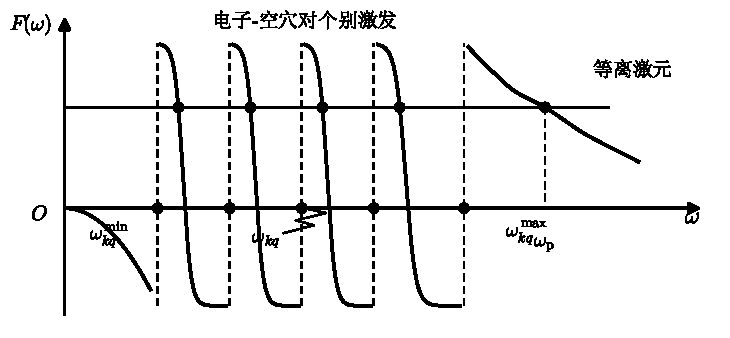
\includegraphics[width=10.5cm]{fig4-3.pdf}\\{\small 图 4.3\quad 确定 $q$ 值时电子系统的元激发 ($q<2k_{\mathrm{F}}$)}
\end{minipage}
\end{center}

这时 $\varepsilon$ 为复量，说明在此区域内不可能存在自发振荡.

对于 $\omega>\omega_{kq}^{\max}$ 的频率区域，式(4.7.2)存在另一支解，这是与 $\omega_{kq}$ 准连续解分离开的解.由于式(4.6.24)中 $\delta$ 函数的宗量在此频区内不可能等于零，故
\begin{equation}
  \mathrm{Im}\,\varepsilon(q,\omega)=\varepsilon_{2}(q,\omega)=0
  \quad\left(\omega>\omega_{kq}^{\max}\right)
\end{equation}
这时介电函数的虚部为零，说明振荡是无阻尼的.不难证明，这一支解代表电子气体的集体振荡.

\begin{center}
\begin{minipage}{4.5cm}
\centering
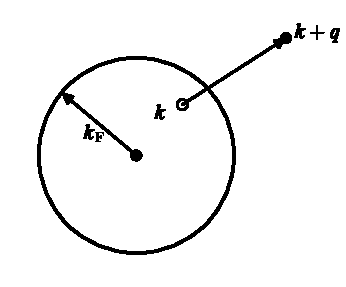
\includegraphics[width=4.5cm]{fig4-4.pdf}\\{\small 图 4.4\quad 电子-空穴对激发}
\end{minipage}
\end{center}

从 $\varepsilon_{1}(q,\omega)=0$ 出发，将式(4.7.2)按 $\left(\dfrac{\omega_{kq}}{\omega}\right)^{2}$ 展开
\begin{equation}
\begin{aligned}
  1=F(\omega)&=\frac{v(q)}{\hbar}\sum_{k}n_{k}
  \frac{4\omega_{kq}}{\omega^{2}-\omega_{kq}^{2}}\\
  &=\frac{v(q)}{\hbar}\sum_{k}n_{k}
  \bigg\{\frac{4\omega_{kq}}{\omega^{2}}+\frac{4\omega_{kq}^{3}}{\omega^{4}}+\cdots\bigg\}
\end{aligned}
\end{equation}
其中 $n_{k}$ 为零温度时费密分布 $2\displaystyle\sum_{k}n_{k}=N\ (n_{k}=n_{-k})$. 因此，准至 $\omega_{kq}$ 的展开式为
\begin{equation}
\begin{aligned}
  1\approx\frac{v(q)}{\hbar}\sum_{k}n_{k}\frac{4\omega_{kq}}{\omega^{2}}
  &=\frac{8\pi e^{2}}{q^{2}}\sum_{k}n_{k}\frac{1}{\omega^{2}}
  \Big(\frac{q^{2}}{m}+2\frac{\boldsymbol{q}\cdot\boldsymbol{k}}{m}\Big)\\
  &=\Big(\frac{4\pi e^{2}N}{m}\Big)\omega^{-2}
  =\Big(\frac{\omega_{\mathrm{p}}}{\omega}\Big)^{2}
\end{aligned}
\end{equation}
由此定出的解为
\begin{equation*}
  \omega\approx\left(\frac{4\pi e^{2}N}{m}\right)^{\frac{1}{2}}=\omega_{\mathrm{p}}
\end{equation*}
它正好就是 $q\to 0$ 时等离子振荡频率.若计及 $\omega_{kq}^{3}$ 项，利用对称性 $n_{k}=n_{-k}$ 可定出准至 $q^{2}$ 的等离子振荡频率
\begin{equation}
  \omega_{q}^{2}=\omega_{\mathrm{p}}^{2}+\frac{3}{5}q^{2}v_{\mathrm{F}}^{2}
  \quad\left(v_{\mathrm{F}}=\frac{\hbar k_{\mathrm{F}}}{m}\right)
\end{equation}
推导时还利用了 $k_{\mathrm{F}}^{3}=3\pi^{2}N$ 和 $n_{k}=\theta(k_{\mathrm{F}}-k)$.由式(4.7.7)求得等离激元的长波限色散关系为
\begin{equation}
  \omega_{q}=\omega_{\mathrm{p}}+\frac{3v_{\mathrm{F}}^{2}}{10\omega_{\mathrm{p}}}\,q^{2}
\end{equation}
当 $q\to 0$ 时，$\omega_{q}=\omega_{\mathrm{p}}\neq 0$，说明三维电子系统的等离子振荡元激发谱中存在相当大的能隙（约为10 eV），它不容易激发.

将个别激发区的边界
\begin{equation*}
\begin{aligned}
  \hbar\omega_{kq}^{\max}&=\frac{\hbar^{2}}{2m}\left(q^{2}+2k_{\mathrm{F}}q\right)\\
  \hbar\omega_{kq}^{\min}&=\left\{\begin{array}{ll}
  0 & (q<2k_{\mathrm{F}})\\[0.3em]
  \dfrac{\hbar^{2}}{2m}\left(q^{2}-2k_{\mathrm{F}}q\right) & (q\geqslant 2k_{\mathrm{F}})
  \end{array}\right.
\end{aligned}
\end{equation*}
和等离激元色散曲线式(4.7.8)在 $\omega$-$q$ 图上绘出，即是§1中的图4.2.图4.5是相同的图，但注明了各区域的 $\varepsilon_{2}$，便于讨论.由图4.5可以看出 $q=q_{c}$ 时集体激发与个别激发相交.当 $q<q_{c}$ 时等离激元的能量 $\hbar\omega_{q}$ 大于电子-空穴对的个别激发能量 $\hbar\omega_{kq}$，这时集体振荡的 $\mathrm{Im}\,\varepsilon=0$，等离激元不衰减为电子-空穴对，反之电子-空穴对也没有足够能量激发等离激元，两者彼此独立，但以集体激发为主.反之当 $q>q_{c}$ 时，由于 $\mathrm{Im}\,\varepsilon\neq 0$，等离子振荡不可能是稳定存在的自发振荡，这时只有个别对的激发.所以，只有在 $0<q<q_{c}$ 范围内才存在集体激发.因此，$q_{c}$ 是等离激元的波矢边界，它是划分个别与集体激发的一个重要参量.

\begin{center}
\begin{minipage}{5.5cm}
\centering
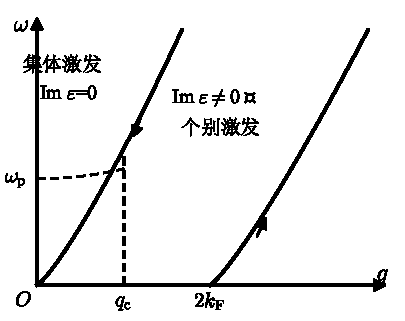
\includegraphics[width=5.5cm]{fig4-5.pdf}\\{\small 图 4.5}
\end{minipage}
\end{center}

比较个别激发和等离激元的色散关系可以估计 $q_{c}$ 的数值，若近似取 $\omega_{q}\approx\omega_{\mathrm{p}}$，则在交点处
\begin{equation*}
  \hbar\omega_{kq}^{\max}=\frac{\hbar^{2}q_{c}^{2}}{2m}
  +\frac{\hbar^{2}q_{c}k_{\mathrm{F}}}{m}
  \approx\hbar v_{\mathrm{F}}q_{c}=\hbar\omega_{\mathrm{p}}
\end{equation*}
可求得
\begin{equation*}
  q_{c}^{2}\approx\left(\frac{\omega_{\mathrm{p}}}{v_{\mathrm{F}}}\right)^{2}
  =\frac{4\pi e^{2}Nm}{\hbar^{2}k_{\mathrm{F}}^{2}}
  =\frac{2\pi Ne^{2}}{E_{\mathrm{F}}}
\end{equation*}
由此算出等离激元的总模数 $N_{\mathrm{p}}=\dfrac{1}{8\pi^{3}}\bigg(\dfrac{4\pi}{3}q_{c}^{3}\bigg)$ 与电子体系的总自由度 $3N$ 之比为
\begin{equation*}
  \frac{N_{\mathrm{p}}}{3N}=\frac{q_{c}^{3}}{6k_{\mathrm{F}}^{3}}
\end{equation*}
对于金属 Na，$\dfrac{N_{\mathrm{p}}}{3N}\approx 18\%$，存在于长波范围内.

金属中的等离子集体振荡是电子间库仑力导致的，由于库仑势场是纵场，因此等离激元是纵振动的量子.等离激元与等离子体不同，等离子体还有横向振荡，地球周围电离层能吸收电磁波就是由于等离子体的横向振荡被激发.

近年来由于人工制成了准二维电子系统（如液氦表面上的电子层和半导体中的 MOS 反型层），引起人们对二维电子体系的研究兴趣.可以利用本章求出的无规相近似介电函数公式计算二维电子体系等离激元的色散曲线，计算时应注意对于二维系统电子间库仑作用的傅里叶分量不再是 $\left(4\pi e^{2}/q^{2}\right)$，而是
\begin{equation}
  v_{\mathrm{2D}}(q)=\frac{2\pi e^{2}}{q}
\end{equation}
它仅与 $q^{-1}$ 成正比.将 $v_{\mathrm{2D}}(q)$ 代入式(4.7.5)，并对二维系统作类似式(4.7.6)、(4.7.7)的近似，可求得二维电子系统等离激元的长波色散关系
\begin{equation}
  \omega_{q}^{2}=\left(\frac{2\pi Ne^{2}}{m}\right)q+\frac{3}{4}q^{2}v_{\mathrm{F}}^{2}
\end{equation}
其中 $N$ 代表电子的面密度.显然
\begin{equation}
  \omega_{q}=\left(\frac{2\pi Ne^{2}}{m}\right)^{1/2}\sqrt{q}
  +o\left(q^{3/2}\right)
\end{equation}
与式(4.7.8)相比较可知二维系统的等离激元是无能隙的，它很容易激发，公式(4.7.11)已为实验所证实.

由于这类人造准二维系统的电子密度有相当大的调节范围，它给机理性研究提供了方便，并取得了较大的进展.例如，长期未观测到的维格纳晶格已在液氦表面的电子层中被证实\textsuperscript{[5]}.此外，半导体中还发现二维电子体系在强磁场作用下会出现分数量子霍尔效应等反常现象\textsuperscript{[6]}，从而为理论工作者提出了新的研究课题.

\section{静电屏蔽}

\subsection*{1. 屏蔽势}

静态外扰动属于介电函数的 $\omega=0$ 情况.根据式(4.6.24)，静态介电函数的虚部满足条件 $\mathrm{Im}\,\varepsilon(q,0)=0$，只有实部的贡献.因此，静态介电函数完全由式(4.6.23)决定：
\begin{equation}
\begin{aligned}
  \varepsilon(q,0)&=\mathrm{Re}\,\varepsilon(q,0)=\varepsilon_{1}(q,0)\\
  &=1+v(q)\sum_{k}\frac{4n_{k}}{\hbar\omega_{kq}}\\
  &=1+\frac{4\pi e^{2}}{q^{2}}\sum_{k<k_{\mathrm{F}}}
  \frac{4}{E_{k+q}-E_{k}}
\end{aligned}
\end{equation}
这个积分可直接算出
\begin{equation}
  \varepsilon_{1}(q,0)=1+\frac{4\pi e^{2}}{q^{2}}\,
  \frac{N}{\frac{2}{3}E_{\mathrm{F}}}
  \bigg\{\frac{1}{2}+\frac{4k_{\mathrm{F}}^{2}-q^{2}}{8k_{\mathrm{F}}q}
  \ln\bigg|\frac{2k_{\mathrm{F}}+q}{2k_{\mathrm{F}}-q}\bigg|\bigg\}
\end{equation}
其中 $E_{\mathrm{F}}$ 为费密能，先研究 $\varepsilon_{1}(q,0)$ 的长波情况；当 $q\ll 2k_{\mathrm{F}}$ 时，将上式对 $(q/2k_{\mathrm{F}})$ 作小量展开，得到介电函数的长波近似式
\begin{equation}
  \varepsilon_{1}(q,0)\approx 1+\left(\frac{6\pi Ne^{2}}{E_{\mathrm{F}}}\right)\frac{1}{q^{2}}
  \equiv 1+\frac{\lambda^{2}}{q^{2}}
\end{equation}
\begin{equation}
  \lambda^{2}=\frac{6\pi Ne^{2}}{E_{\mathrm{F}}}=3q_{c}^{2}
\end{equation}
式(4.8.3)称为托马斯-费密（Thomas-Fermi）介电函数.现在利用此近似式讨论原点处有一个 $(-e)$ 的电荷的屏蔽情况.这时，外扰动势的傅里叶分量为 $V_{\mathrm{e}}(q)=\dfrac{4\pi e^{2}}{q^{2}}=v(q)$，利用托马斯-费密介电函数和式(4.6.30)得到 $(V_{\mathrm{e}}/V)=\varepsilon$，可求总势能的傅里叶分量
\begin{equation}
  V_{\mathrm{TF}}(q)=\frac{V_{\mathrm{e}}(q)}{\varepsilon_{1}(q,0)}
  =\frac{4\pi e^{2}}{q^{2}+\lambda^{2}}
\end{equation}
而总势能的托马斯-费密公式为
\begin{equation}
  V_{\mathrm{TF}}(r)=\sum_{\boldsymbol{q}}\frac{4\pi e^{2}}{q^{2}+\lambda^{2}}
  \mathrm{e}^{\mathrm{i}\boldsymbol{q}\cdot\boldsymbol{r}}
  =\frac{e^{2}}{r}\,\mathrm{e}^{-\lambda r}
\end{equation}
上式表明，一个位于原点的 $(-e)$ 电荷将在 $\lambda^{-1}$ 距离内被屏蔽.由此不难推论，电子体系的屏蔽效应使金属中电子间的库仑互作用 $(e^{2}/r)$ 变为汤川（Yukawa）型互作用 $(e^{2}/r)\exp(-\lambda r)$，这里 $\lambda$ 与 $q_{c}$ 同量级，$q_{c}$ 是等离激元波数的上限.在玻姆-派因斯（Bohm-Pines）的早期理论中\textsuperscript{[7]}是从另一角度讨论屏蔽作用的.他们曾用幺正变换方法将库仑势傅里叶展开的长波部分 $(0<q<q_{c})$ 表示为等离子集体振荡，用于产生等离激元.这样，在库仑势中自然只剩下短波成分 $(q>q_{c})$，从而使个别电子间互作用成为短程屏蔽势.因为库仑作用的短波部分可写为
\begin{equation}
\begin{aligned}
  V_{\mathrm{SR}}(r)&=\sum_{q>q_{c}}\frac{4\pi e^{2}}{q^{2}}
  \mathrm{e}^{\mathrm{i}\boldsymbol{q}\cdot\boldsymbol{r}}
  =\frac{e^{2}}{2\pi}\int_{q>q_{c}}\frac{\mathrm{e}^{\mathrm{i}\boldsymbol{q}\cdot\boldsymbol{r}}}{q^{2}}\,\mathrm{d}^{3}q\\
  &=\frac{e^{2}}{r}\bigg\{1-\frac{2}{\pi}\int_{0}^{q_{c}r}
  \frac{\sin qr}{qr}\,\mathrm{d}(qr)\bigg\}\\
  &=\frac{e^{2}}{r}\bigg\{1-\frac{2}{\pi}\mathrm{Si}\left(q_{c}r\right)\bigg\}
\end{aligned}
\end{equation}
其中积分函数定义为
\begin{equation}
  \mathrm{Si}\left(q_{c}r\right)\equiv\int_{0}^{q_{c}r}\frac{\sin x}{x}\,\mathrm{d}x
\end{equation}
当 $q_{c}r\to\infty$ 时函数 $\mathrm{Si}(q_{c}r)\to\dfrac{\pi}{2}$，说明 $V_{\mathrm{SR}}$ 的作用局限在 $\left(1/q_{c}\right)$ 尺度之内，它和 $V_{\mathrm{TF}}$ 的屏蔽趋势基本相同.因此，扣除了集体振荡后，只剩下电子间的短程屏蔽互作用，好像在每个电子周围附加了一个半径约为 $\left(1/q_{c}\right)$ 的正电屏蔽壳层.从微观角度分析；由于关联效应，电子将排开周围电子，形成随电子运动的正电“空穴云”，施里弗（Schrieffer）称其为相关空穴，这种相关效应不仅表现为对电荷的屏蔽，还将产生运动学修正表现为改变电子的有效质量，并导致有限的寿命，我们将在§11中作专门的讨论.计及了这些修正的电子，实际上已经和多电子系统分不开了，只能认为是多体系统中的准粒子，这类准粒子被称为准电子.因此，我们应当把等离激元和准电子理解为互作用电子系统集体效应的两个方面.

\subsection*{2. 孔恩异常}

以上讨论的汤川型互作用只是式(4.8.2)取长波极限的近似公式.当研究晶体中杂质和缺陷对于电子和声子谱的影响时，往往需要更严格的公式，这时应当从式(4.8.2)出发，并将它改写为
\begin{equation}
  \left.\begin{aligned}
  \varepsilon_{1}(q,0)&=1+\frac{\lambda^{2}}{q^{2}}S\left(q/2k_{\mathrm{F}}\right)\\
  S(x)&\equiv\frac{1}{2}\bigg[1+\frac{1-x^{2}}{2x}
  \ln\bigg|\frac{1+x}{1-x}\bigg|\bigg]
  \end{aligned}\right\}
\end{equation}
当 $q\to 0$ 时 $S\to 1$，当 $q$ 很大时 $S\to 0$. 但在 $q=2k_{\mathrm{F}}$ 时，$\dfrac{\partial S}{\partial q}$ 发散，$S$ 函数有 $(q-2k_{\mathrm{F}})\ln\left(q-2k_{\mathrm{F}}\right)$ 型的对数奇性.图4.6是屏蔽参数 $\lambda^{2}S$ 随 $q$ 的变化曲线，静态介电函数在 $q=2k_{\mathrm{F}}$ 点也有相似变化.屏蔽参数及介电函数在 $q=2k_{\mathrm{F}}$ 处的突然下降是由于电子气的基态分布在费密能量上有不连续性，而费密球的直径恰好为 $2k_{\mathrm{F}}$. 更具体的说明如下：

比较式(4.8.1)和(4.8.9)有
\begin{equation}
  \lambda^{2}S\left(q/2k_{\mathrm{F}}\right)=4v(q)q^{2}
  \sum_{k<k_{\mathrm{F}}}\frac{1}{\left(E_{k+q}-E_{k}\right)}
\end{equation}
显然，$\lambda^{2}S$ 的大小与能量分母 $\left(E_{k+q}-E_{k}\right)$ 有关，这里 $\boldsymbol{k}$ 为费密球内已被占据态，只要 $|\boldsymbol{q}|<2k_{\mathrm{F}}$，我们总可以作出一个矢量 $\boldsymbol{q}$，使 $\boldsymbol{k}$ 与 $\boldsymbol{k}+\boldsymbol{q}$ 都落在费密面附近，因此式(4.8.10)中总有一些项的能量分母较小.所以，当 $|\boldsymbol{q}|<2k_{\mathrm{F}}$ 时，$\lambda^{2}S$ 和 $\varepsilon$ 都比较大.但是，当 $|\boldsymbol{q}|\geqslant 2k_{\mathrm{F}}$ 时，由于 $|\boldsymbol{q}|$ 已超过费密球直径 $2k_{\mathrm{F}}$，上述可能性消失，式(4.8.10)中各项的能量分母都比较大，因此，在 $q=2k_{\mathrm{F}}$ 处屏蔽参数和介电函数将突然下降.

\begin{center}
\begin{minipage}{5cm}
\centering
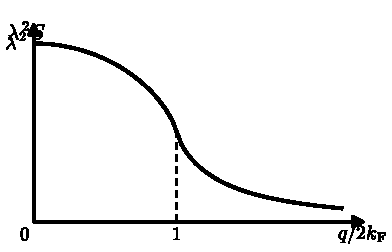
\includegraphics[width=5cm]{fig4-6.pdf}\\{\small 图 4.6}
\end{minipage}
\end{center}

介电函数和在 $q=2k_{\mathrm{F}}$ 点的奇性，对于声子谱有重要影响.金属晶格中离子的振动可看作电子的一个扰动势场，而电子对此扰动场的响应又将反过来屏蔽离子势，使离子间有效互作用减弱，并导致晶格振动频率下降.因此，介电函数在 $2k_{\mathrm{F}}$ 处的奇性也必然会反映在声子的 $\omega(q)$ 曲线上.实验已观察到，在三维金属 Pb 中 $q=2k_{\mathrm{F}}$ 的声子频率有软化现象，并称之为孔恩异常（Kohn anomalies）.近年来又发现，在链状固体 KCP 和 TTF-TCNQ 中，当温度趋于某临界值时，$2k_{\mathrm{F}}$ 声子频率将突然下降到很小的数值（接近零）\textsuperscript{[8]}.这种 $2k_{\mathrm{F}}$ 声子的完全软化现象称为强孔恩异常，它是一维系统中电子元激发特征的反映.一维系统的电子-空穴对激发区与二维或三维系统有本质区别，其个别对激发 $\hbar\omega_{kq}=E_{k+q}-E_{k}\ (|k|<k_{\mathrm{F}},\,|k+q|>k_{\mathrm{F}})$ 仅在图4.7的（Ⅰ）区中出现.（Ⅱ）区中不存在 $\omega_{kq}$ 激发，是一维系统个别激发的空隙区.因此，一维系的声子色散曲线（Ⅲ）只能在 $2k_{\mathrm{F}}$ 附近与电子系统的个别激发谱相交，这时费密面上的电子将通过 $k_{\mathrm{F}}\to(-k_{\mathrm{F}})$ 的对端跃迁吸收或发射 $2k_{\mathrm{F}}$ 声子，使声子谱中 $2k_{\mathrm{F}}$ 波矢附近的晶格离子振动受到电子系统的强烈屏蔽，并产生 $2k_{\mathrm{F}}$ 声子的明显软化效应，这就是链状固体中出现强孔恩异常的物理实质.

\begin{center}
\begin{minipage}{6cm}
\centering
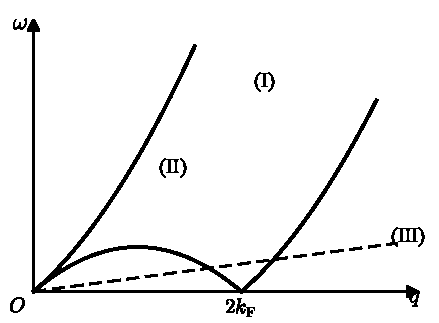
\includegraphics[width=6cm]{fig4-7.pdf}\\{\small 图 4.7\quad 一维系中电子与声子谱的共振特征}\\[0.2em]
{\small （Ⅰ）电子-空穴对激发区；（Ⅱ）个别激发的空隙区；（Ⅲ）声子色散曲线}
\end{minipage}
\end{center}

\subsection*{3. 夫里德耳振荡}

现在利用静态介电函数讨论金属中电子对杂质（或点缺陷）的屏蔽作用.设杂质位于原点并带有 $Ze$ 电荷，则杂质受电子体系屏蔽的有效势能为
\begin{equation}
  V(\boldsymbol{r})=-\sum_{\boldsymbol{q}}
  \frac{4\pi Ze^{2}}{\varepsilon_{1}(q,0)\,q^{2}}
  \mathrm{e}^{\mathrm{i}\boldsymbol{q}\cdot\boldsymbol{r}}
\end{equation}
将严格公式(4.8.9)代入上式得
\begin{equation}
  V(\boldsymbol{r})=-\frac{1}{8\pi^{3}}\int
  \frac{4\pi Ze^{2}}{q^{2}+\lambda^{2}S\left(q/2k_{\mathrm{F}}\right)}
  \mathrm{e}^{\mathrm{i}\boldsymbol{q}\cdot\boldsymbol{r}}\,\mathrm{d}^{3}q
\end{equation}
这个积分可用近似方法计算\textsuperscript{[9]}，在 $r$ 很大时有渐近式
\begin{equation}
  V(r)\sim\frac{\cos 2k_{\mathrm{F}}r}{r^{3}}
\end{equation}
上式代表一个以 $2k_{\mathrm{F}}$ 为波数的振荡势能，称为夫里德耳（Friedel）振荡势.图4.8对夫里德耳振荡势和汤川势型屏蔽势作了比较，两者有相同的屏蔽趋势，但差别在于长程振荡.

\begin{center}
\begin{minipage}{5.5cm}
\centering
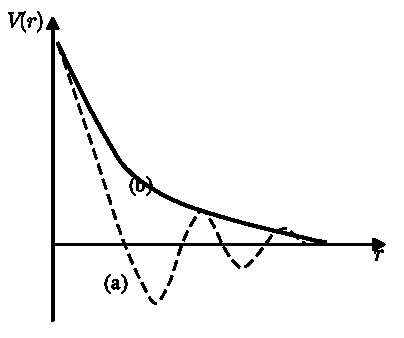
\includegraphics[width=5.5cm]{fig4-8.pdf}\\{\small 图 4.8\quad (a) 夫里德耳振荡势；(b) 汤川势}
\end{minipage}
\end{center}

再看杂质周围屏蔽电子数密度 $\Delta\rho(r)$ 的空间分布，从泊松方程出发
\begin{equation}
  \nabla^{2}V(r)=4\pi e^{2}\left\{Z\delta(r)-\Delta\rho(r)\right\}
\end{equation}
将 $V(r)$ 的严格式(4.8.11)代入，求得
\begin{equation}
  \Delta\rho(\boldsymbol{r})=\frac{Z}{8\pi^{3}}\int
  \left(1-\frac{1}{\varepsilon_{1}(q,0)}\right)
  \mathrm{e}^{\mathrm{i}\boldsymbol{q}\cdot\boldsymbol{r}}\,\mathrm{d}^{3}q
\end{equation}
当 $r\to\infty$ 时，$\Delta\rho$ 的渐近式为
\begin{equation}
  \Delta\rho(r)\sim\frac{\cos 2k_{\mathrm{F}}r}{r^{3}}
\end{equation}
说明在杂质周围屏蔽电荷的分布也具有长程振荡特征，这就是著名的夫里德耳振荡.如果用汤川势代入泊松方程，则 $\Delta\rho$ 变为
\begin{equation}
  \Delta\rho(r)\sim\frac{Z\lambda^{2}}{4\pi}\,\frac{\mathrm{e}^{-\lambda r}}{r}
\end{equation}
与式(4.8.16)相比较，屏蔽电荷失去了长程振荡特性，这是因为汤川势来源于对 $S\left(q/2k_{\mathrm{F}}\right)$ 取长波近似，它只是准经典理论的结果，实际上不能充分反映电子系统的量子效应.

产生夫里德耳振荡的原因主要是由于金属中电子有明确的费密面.正如前面讨论孔恩异常时的分析，由于 $T=0$ K 时电子分布严格限制在 $|k|=k_{\mathrm{F}}$ 球内，静态介电函数 $\varepsilon_{1}(q,0)$ 将在 $q=2k_{\mathrm{F}}$ 处有突然下降，$\varepsilon_{1}(q,0)$ 的这个奇异性使积分式(4.8.15)的主要贡献来源于 $q=2k_{\mathrm{F}}$ 项，从而得到 $\Delta\rho$ 与 $V(r)$ 都以 $2k_{\mathrm{F}}$ 波数振荡的结果.从物理观点分析，金属中参加屏蔽的粒子主要是费密面上的电子，由于这些电子的德布罗意波在杂质上的衍射效应，使围绕杂质的屏蔽电荷分布起振荡变化，从而形成与小孔衍射光圈图相似的 $\Delta\rho(r)$ 分布图案.夫里德耳指出\textsuperscript{[10]}，这时在杂质周围不是形成一个（或两个）电子的束缚态，而是费密面上电子在杂质势阱中形成共振态并具有有限寿命.关于共振散射态理论，我们将在第十一章中讨论局域磁矩时用格林函数方法作介绍，其初级理论可参阅有关量子力学书籍（例如第一章文献[3]p235）.

\section{基态能}

互作用电子体系的基态能直接关系到金属结合能的定量估计，是固体理论的重要问题.但是，过去基态能只有哈特利-福克近似（HFA）的计算结果，进一步的微扰修正，由于涉及长程库仑力，遇到了发散困难.直到等离激元理论问世以后，人们才认识到应当在集体振荡的基础上用屏蔽库仑势作计算，从而克服了库仑势长程部分带来的发散困难，使基态能的研究进入定量计算阶段.本节首先介绍基态能的哈特利-福克近似计算及其存在的困难，然后再利用介电函数导出基态能的严格公式，并给出高密度电子体系基态能的计算结果.

\subsection*{1. 哈特利-福克近似的基态能}

对于互作用电子体系哈密顿量
\begin{equation}
  H=H_{0}+H'=\sum_{k,\sigma}\frac{\hbar^{2}k^{2}}{2m}C_{k\sigma}^{+}C_{k\sigma}
  +\frac{1}{2}\mathop{{\sum}'}\limits_{q}v(q)\left(\rho_{q}^{+}\rho_{q}-N\right)
\end{equation}
的一阶微扰计算叫哈特利-福克近似.因此，在哈特利-福克近似范围内只需用无相互作用电子系的基态（费密球状态）
\begin{equation}
  |0\rangle_{0}=\prod_{k\sigma}C_{k\sigma}^{+}\ |\ \mathrm{Vac}\rangle
\end{equation}
对 $H$ 求对角平均.其中 $|\mathrm{Vac}\rangle$ 代表 $k$ 空间全部未被占据的状态，即真正的真空态.

哈特利-福克近似的基态能
\begin{equation}
  E_{0}\left(\mathrm{HFA}\right)=E_{k}+E_{\mathrm{ex}}
\end{equation}
其中
\begin{equation}
\begin{aligned}
  E_{\mathrm{K}}={}_{0}\langle 0|H_{0}|0\rangle_{0}
  &=\sum_{k,\sigma}\frac{\hbar^{2}k^{2}}{2m}\,
  {}_{0}\langle 0|C_{k\sigma}^{+}C_{k\sigma}|0\rangle_{0}\\
  &=2\sum_{k}\frac{\hbar^{2}k^{2}}{2m}\theta\left(k_{\mathrm{F}}-k\right)
  =\frac{3}{5}NE_{\mathrm{F}}
\end{aligned}
\end{equation}
代表电子体系的总动能，$E_{\mathrm{F}}=\left(\hbar^{2}k_{\mathrm{F}}^{2}/2m\right)$ 为费密能，而
\begin{equation}
\begin{aligned}
  E_{\mathrm{ex}}&={}_{0}\langle 0|H'|0\rangle_{0}
  =\frac{1}{2}\mathop{{\sum}'}\limits_{q}v(q)
  \left({}_{0}\langle 0|\rho_{q}^{+}\rho_{q}|0\rangle_{0}-N\right)\\
  &=\frac{1}{2}\mathop{{\sum}'}\limits_{q}v(q)\sum_{k_{1},k_{2}}\sum_{\sigma_{1},\sigma_{2}}
  {}_{0}\langle 0|C_{k_{1}+q,\sigma_{1}}^{+}C_{k_{2}-q,\sigma_{2}}^{+}
  C_{k_{2}\sigma_{2}}C_{k_{1}\sigma_{1}}|0\rangle_{0}\\
  &=-\sum_{k_{1}}\sum_{k_{2}}
  \frac{4\pi e^{2}}{|k_{1}-k_{2}|^{2}}
  \theta\left(k_{\mathrm{F}}-k_{1}\right)\theta\left(k_{\mathrm{F}}-k_{2}\right)
\end{aligned}
\end{equation}
由于 $q\neq 0$，因此在上式中只有 $\boldsymbol{k}_{2}=\boldsymbol{k}_{1}+\boldsymbol{q}$，$\sigma_{2}=\sigma_{1}$ 项的贡献，它代表自旋平行电子之间的交换能.式(4.9.5)的计算是直截了当的，可令
\begin{equation}
  E_{\mathrm{ex}}=\sum_{k_{1}}\theta\left(k_{\mathrm{F}}-k_{1}\right)
  \mathcal{E}_{\mathrm{ex}}\left(k_{1}\right)
\end{equation}
这里 $\mathcal{E}_{\mathrm{ex}}$ 是单电子的自能修正
\begin{equation}
\begin{aligned}
  \mathcal{E}_{\mathrm{ex}}(\boldsymbol{k}_{1})
  &=-\sum_{k_{2}}\frac{4\pi e^{2}}{|\boldsymbol{k}_{1}-\boldsymbol{k}_{2}|^{2}}
  \theta\left(k_{\mathrm{F}}-k_{2}\right)\\
  &=\frac{e^{2}}{\pi}\int_{0}^{k_{\mathrm{F}}}k_{2}^{2}\,\mathrm{d}k_{2}
  \int_{-1}^{1}\frac{\mathrm{d}\mu}{k_{1}^{2}+k_{2}^{2}-2k_{1}k_{2}\mu}
  =-\frac{2e^{2}}{\pi}k_{\mathrm{F}}S(x)
\end{aligned}
\end{equation}
其中 $x\equiv\left(k_{1}/k_{\mathrm{F}}\right)$
\begin{equation}
  S(x)=\frac{1}{2}\bigg\{1+\frac{1-x^{2}}{2x}
  \ln\bigg|\frac{1+x}{1-x}\bigg|\bigg\}
\end{equation}
代入式(4.9.6)，再将 $\boldsymbol{k}_{1}$ 求和化为积分，算出交换能
\begin{equation}
\begin{aligned}
  E_{\mathrm{ex}}&=-\frac{2e^{2}}{\pi}k_{\mathrm{F}}^{4}\,\frac{1}{8\pi^{3}}
  \int S(x)\,\mathrm{d}^{3}x\\
  &=-\bigg(\frac{3e^{2}}{\pi}k_{\mathrm{F}}\bigg)N\int_{0}^{1}x^{2}S(x)\,\mathrm{d}x\\
  &=-N\bigg(\frac{3e^{2}}{4\pi}\bigg)k_{\mathrm{F}}
\end{aligned}
\end{equation}
其中利用了关系式 $k_{\mathrm{F}}^{3}=3\pi^{2}N$ 和 $S(x)$ 的下列定积分
\begin{equation}
  4\int_{0}^{1}x^{2}S(x)\,\mathrm{d}x=1
\end{equation}
因此，在哈特利-福克近似中平均每个电子的基态能量为
\begin{equation}
  \frac{1}{N}E_{0}\left(\mathrm{HFA}\right)
  =\frac{3}{5}\,\frac{\hbar^{2}k_{\mathrm{F}}^{2}}{2m}
  -\frac{3e^{2}}{4\pi}k_{\mathrm{F}}
\end{equation}
讨论电子体系基态能时常采用量纲为 1 的参量 $r_{s}$ 描述系统的电子密度，其定义为
\begin{equation}
  N\,\frac{4\pi}{3}\left(r_{s}a_{\mathrm{H}}\right)^{3}=1
\end{equation}
其中 $a_{\mathrm{H}}=\dfrac{\hbar^{2}}{me^{2}}$ 是氢原子的第一玻尔轨道半径.由上式可知，$r_{s}a_{\mathrm{H}}$ 代表平均一个电子所占球体之半径，当 $r_{s}<1$ 时称为高密度电子气，反之当 $r_{s}\gg 1$ 属于低密度情况.用 $r_{s}$ 表示的费密波数为
\begin{equation}
  k_{\mathrm{F}}=\left(\frac{9\pi}{4}\right)^{1/3}
  \frac{1}{r_{s}a_{\mathrm{H}}}
\end{equation}
将式(4.9.13)代入式(4.9.11)求得哈特利-福克近似的基态能
\begin{equation}
  \frac{1}{N}E_{0}\left(\mathrm{HFA}\right)
  =\frac{2.21}{r_{s}^{2}}-\frac{0.916}{r_{s}}\quad\left[\mathrm{Ry}\right]
\end{equation}
其中能量用里德伯单位［Ry］
\begin{equation}
  1\ \left[\mathrm{Ry}\right]\equiv\frac{me^{4}}{2\hbar^{2}}
  =\frac{e^{2}}{2a_{\mathrm{H}}}=13.6\ \mathrm{eV}
\end{equation}
上述哈特利-福克近似结果可以定性说明系统的结合，但算出的结合能定量数值明显偏小.例如金属锂（Li）结合能的实验值为 36.5［Ry］而哈特利-福克近似的计算值仅为 17［Ry］.为了改进计算结果，人们曾经尝试计算库仑作用的二阶以及高阶微扰修正，但是都碰到了发散困难.

\subsection*{2. 相关能的二阶微扰计算}

在哈特利-福克近似基础上，计入反平行自旋电子间库仑作用所降低的能量称为相关能，最低阶的相关能可利用二阶微扰公式
\begin{equation}
  E^{(2)}=-\mathop{{\sum}'}\limits_{n}
  \frac{\left|\,{}_{0}\langle 0|H'|n\rangle_{0}\right|^{2}}{E_{n}-E_{0}}
\end{equation}
求出，其中 $|n\rangle_{0}$ 为中间态，求和的限制是 $E_{n}\neq E_{0}$. 先讨论一对 $\boldsymbol{k}_{1}\uparrow$ 与 $\boldsymbol{k}_{2}\downarrow$ 电子经 $H'$ 散射到中间态 $\boldsymbol{k}_{3}\uparrow$ 与 $\boldsymbol{k}_{4}\downarrow$，并将初态 $|0\rangle_{0}$ 记为 $|12\rangle$，而中间态则用 $|34\rangle$ 表示.根据泡利原理，$\boldsymbol{k}_{1}$ 与 $\boldsymbol{k}_{2}$ 必须位于费密球内，而 $\boldsymbol{k}_{3}$ 与 $\boldsymbol{k}_{4}$ 均应在球外，这时 1 与 2 电子之间的直接互作用项为
\begin{equation}
  E_{\mathrm{c}}^{(2)}\left(k_{1},k_{2}\right)
  =-\left(\frac{2m}{\hbar^{2}}\right)\sum_{k_{3}}\sum_{k_{4}}
  \frac{\langle 12|H'|34\rangle\langle 34|H'|12\rangle}
  {\left[\left(k_{3}^{2}+k_{4}^{2}\right)-\left(k_{1}^{2}+k_{2}^{2}\right)\right]}
  \left(1-n_{k_{3}}\right)\left(1-n_{k_{4}}\right)
\end{equation}
其中 $n_{k_{3}}=\theta\left(k_{\mathrm{F}}-k_{3}\right)$，$\left(1-n_{k_{3}}\right)\left(1-n_{k_{4}}\right)$ 因子的出现保证了 $\boldsymbol{k}_{3}$ 与 $\boldsymbol{k}_{4}$ 电子均在费密球外.当取体积 $V=1$ 时，微扰矩阵元为
\begin{equation}
  \langle 34|H'|12\rangle=\frac{4\pi e^{2}}{q^{2}}\,
  \delta_{\boldsymbol{k}_{1}+\boldsymbol{k}_{2},\,\boldsymbol{k}_{3}+\boldsymbol{k}_{4}}
\end{equation}
散射的动量守恒条件可用波矢 $\boldsymbol{q}$ 的下列等式表示
\begin{equation}
  \boldsymbol{q}\equiv\boldsymbol{k}_{1}-\boldsymbol{k}_{3}
  =\boldsymbol{k}_{4}-\boldsymbol{k}_{2}
\end{equation}
从而得到 $\boldsymbol{k}_{3}=\boldsymbol{k}_{1}-\boldsymbol{q}$ 与 $\boldsymbol{k}_{4}=\boldsymbol{k}_{2}+\boldsymbol{q}$.由于 $\boldsymbol{k}_{3}$ 与 $\boldsymbol{k}_{4}$ 并不独立，可改用波矢 $\boldsymbol{q}$，将式(4.9.17)改写为
\begin{equation}
  E_{\mathrm{c}}^{(2)}\left(k_{1},k_{2}\right)
  =-\left(\frac{2m}{\hbar^{2}}\right)\mathop{{\sum}'}\limits_{q}
  \left(\frac{4\pi e^{2}}{q^{2}}\right)^{2}
  \frac{\left(1-n_{k_{1}-q}\right)\left(1-n_{k_{2}+q}\right)}
  {\left[q^{2}+q\cdot\left(k_{2}-k_{1}+q\right)\right]}
\end{equation}
上式对 $\boldsymbol{k}_{1}$ 与 $\boldsymbol{k}_{2}$ 求和后，得到总的二阶修正
\begin{equation}
\begin{aligned}
  E_{\mathrm{c}}^{(2)}&=\sum_{k_{1}}\sum_{k_{2}}E_{\mathrm{c}}^{(2)}\left(k_{1},k_{2}\right)\\
  &=-\sum_{k_{1},k_{2}}\mathop{{\sum}'}\limits_{q}
  \left(\frac{2m}{\hbar^{2}}\right)\left(\frac{4\pi e^{2}}{q^{2}}\right)^{2}
  \frac{n_{k_{1}}\left(1-n_{k_{1}-q}\right)\left(1-n_{k_{2}+q}\right)}
  {\left[q^{2}+q\cdot\left(k_{2}-k_{1}+q\right)\right]}
\end{aligned}
\end{equation}
为了便于运算和将 $E_{\mathrm{c}}^{(2)}$ 用里德伯单位 $\left(e^{2}/2a_{\mathrm{H}}\right)$ 量度，作下列变量代换：
\begin{equation}
  \boldsymbol{k}_{1}\to-\boldsymbol{p}k_{\mathrm{F}},\quad
  \boldsymbol{k}_{2}\to\boldsymbol{k}k_{\mathrm{F}},\quad
  \boldsymbol{q}\to\boldsymbol{q}k_{\mathrm{F}}
\end{equation}
使所有波矢的量纲均为 1，再考虑到系统为各向同性时 $\boldsymbol{n}_{-p}=\boldsymbol{n}_{p}=\theta\left(1-p\right)$，可将相关能的修正写为
\begin{equation}
  E_{\mathrm{c}}^{(2)}=\left(\frac{Ne^{2}}{2a_{\mathrm{H}}}\right)
  \varepsilon_{\mathrm{c}}^{(2)}
\end{equation}
其中
\begin{equation}
  \varepsilon_{\mathrm{c}}^{(2)}=-\left(\frac{3}{8\pi^{5}}\right)
  \int\frac{\mathrm{d}^{3}q}{q^{4}}\,f(\boldsymbol{q})
\end{equation}
\begin{equation}
  f(\boldsymbol{q})=\int\mathrm{d}^{3}p\int\mathrm{d}^{3}k\,
  \frac{\theta\left(1-p\right)\left[1-\theta\left(1-|\boldsymbol{p}+\boldsymbol{q}|\right)\right]
  \theta\left(1-k\right)\left[1-\theta\left(1-|\boldsymbol{k}+\boldsymbol{q}|\right)\right]}
  {\left[q^{2}+\boldsymbol{q}\cdot\left(\boldsymbol{p}+\boldsymbol{k}+\boldsymbol{q}\right)\right]}
\end{equation}
$\varepsilon_{\mathrm{c}}^{(2)}$ 代表在里德伯单位中平均每个格点的二阶修正能量.显然，对 $\varepsilon_{\mathrm{c}}^{(2)}$ 的主要贡献来自长波 $(q\to 0)$ 部分.为此，先作长波近似，讨论 $q\to 0$ 时 $\varepsilon_{\mathrm{c}}^{(2)}$ 的渐近行为.当 $\boldsymbol{q}\to 0$ 时，阶跃函数中的 $q^{2}$ 项可略去，有长波近似式
\begin{equation}
  \theta\left(1-|\boldsymbol{p}+\boldsymbol{q}|\right)=\theta\left(1-p\right)
  -\left(\boldsymbol{q}\cdot\boldsymbol{p}/p\right)\delta\left(1-p\right)
\end{equation}
由此求得在长波近似下泡利原理对 $\boldsymbol{p}$ 电子激发的一个限制
\begin{subequations}
\begin{equation}
\begin{aligned}
  \theta\left(1-p\right)\left[1-\theta\left(|\boldsymbol{p}+\boldsymbol{q}|\right)\right]
  &=\theta\left(1-p\right)\left\{\left[1-\theta\left(1-p\right)\right]
  +\left(\boldsymbol{q}\cdot\boldsymbol{p}/p\right)\delta\left(1-p\right)\right\}\\
  &=\theta\left(1-p\right)\delta\left(1-p\right)
  \left(\boldsymbol{q}\cdot\boldsymbol{p}/p\right)\geqslant 0
\end{aligned}
\end{equation}
其中利用了阶跃函数的 $\theta(x)\left[1-\theta(x)\right]=0$ 特征.上式在物理上表明，在长波近似下互作用激发的电子仅限于费密面 $(p=1)$ 附近极薄的壳层内，其厚度正比于 $\boldsymbol{q}$. 此外，上式还限定 $\boldsymbol{p}\cdot\boldsymbol{q}\geqslant 0$，此即要求 $\boldsymbol{p}$ 与 $\boldsymbol{q}$ 间的夹角余弦 $y=\cos\theta_{pq}\geqslant 0$，此限制也可从泡利原理所要求的 $p\leqslant 1$ 和 $|\boldsymbol{p}+\boldsymbol{q}|\geqslant 1$，在长波近似下略去 $q^{2}$ 项后直接导出.因此，在长波近似下，泡利原理对 $\boldsymbol{p}$ 电子激发的另一限制是
\begin{equation}
  0\leqslant y\leqslant 1
\end{equation}
\end{subequations}
对于 $k$ 电子，也存在相同的限制，这时可将 $f(\boldsymbol{q})$ 表示式分母中 $q^{2}$ 项略去，积分后求得
\begin{subequations}
\begin{equation}
  \lim_{q\to 0}f(\boldsymbol{q})=(2\pi)^{2}Iq
\end{equation}
其中
\begin{equation}
  I\equiv\int_{0}^{1}\mathrm{d}y\int_{0}^{1}\mathrm{d}z\,
  \frac{yz}{y+z}=\frac{2}{3}\left(1-\ln 2\right)
\end{equation}
\end{subequations}
这样就求出了相关能 $\varepsilon_{\mathrm{c}}^{(2)}$ 的长波特性
\begin{equation}
  \lim_{q\to 0}\varepsilon_{\mathrm{c}}^{(2)}
  =-\bigg(\frac{4}{\pi^{2}}\bigg)\left(1-\ln 2\right)\int\frac{\mathrm{d}q}{q}
  \sim-\ln q
\end{equation}
显然，当 $q\to 0$ 时 $\varepsilon_{\mathrm{c}}^{(2)}$ 呈现对数式发散.但是，在大 $\boldsymbol{q}$ 情况下 $(q\gg 2k_{\mathrm{F}}$ 时$)$，由于式(4.9.25)分母中 $\boldsymbol{q}\cdot(\boldsymbol{p}+\boldsymbol{k})$ 项可略去，并且当 $q>2k_{\mathrm{F}}$ 时，总有 $\theta\left(1-|\boldsymbol{p}+\boldsymbol{q}|\right)=0$ 和 $\theta\left(1-|\boldsymbol{k}+\boldsymbol{q}|\right)=0$，将使 $f(\boldsymbol{q})$ 的积分简化为
\begin{subequations}
\begin{equation}
  \lim_{q\to\infty}f(q)=\int\mathrm{d}^{3}p\int\mathrm{d}^{3}k\,
  \theta\left(1-p\right)\theta\left(1-k\right)
  =\left(\frac{4\pi}{3}\right)^{2}/q^{2}
\end{equation}
由此求出 $\varepsilon_{\mathrm{c}}^{(2)}$ 在 $q\to\infty$ 时的特征为
\begin{equation}
  \lim_{q\to\infty}\varepsilon_{\mathrm{c}}^{(2)}
  =-\frac{3}{8\pi^{5}}\int\mathrm{d}^{3}q\;q^{-4}\lim_{q\to\infty}f(q)
  =\frac{8}{3\pi^{2}}\,q^{-3}
\end{equation}
\end{subequations}
它按照 $\boldsymbol{q}^{-3}$ 趋于零，是收敛的.

根据以上讨论可知，用微扰论计算相关能的主要困难来自长波部分存在 ln $q$ 型的对数式发散.类似的长波发散还出现在三阶以至所有高阶的微扰计算之中，这是建立金属基态能理论的主要困难.

微扰理论之所以产生相关能发散的困难是因为没有考虑互作用对电子态的影响（即多体效应）\nobreak.因此，为了消除发散，必须在集体运动的基础上考虑屏蔽效应，下面将从多体系统的介电函数理论出发，推导基态能的严格公式.

\subsection*{3. 基态能的严格公式——费因曼定理}

利用附录B中严格介电函数公式(B.14)
\begin{equation}
  \mathrm{Im}\bigg[\frac{1}{\varepsilon(q,\omega)}\bigg]
  =\frac{\pi v(q)}{\hbar}\sum_{n}
  |\langle n|\rho_{q}|0\rangle|^{2}
  \left[\delta\left(\omega+\omega_{n0}\right)-\delta\left(\omega-\omega_{n0}\right)\right]
\end{equation}
其中
\begin{equation}
  \omega_{n0}\equiv\frac{1}{\hbar}\left(\mathcal{E}_{n}-\mathcal{E}_{0}\right)
\end{equation}
$|n\rangle$ 和 $\mathcal{E}_{n}$ 为多体系 $H$ 的严格本征态和能量本征值，$|0\rangle$ 代表严格基态.

利用 $\mathrm{Im}\bigg[\dfrac{1}{\varepsilon(q,\omega)}\bigg]$ 既可以计算库仑相互作用能量，也能求出互作用电子系统的基态能量.

式(4.9.31)对 $\omega$ 积分，考虑到 $\omega_{n0}>0$，应有
\begin{equation}
\begin{aligned}
  \int_{0}^{\infty}\mathrm{d}\omega\,
  \mathrm{Im}\bigg[\frac{1}{\varepsilon(q,\omega)}\bigg]
  &=-\frac{4\pi^{2}e^{2}}{q^{2}\hbar}\sum_{n}
  |\langle n|\rho_{q}|0\rangle|^{2}\\
  &=-\frac{\pi v(q)}{\hbar}\langle 0|\rho_{q}^{+}\rho_{q}|0\rangle
\end{aligned}
\end{equation}
由于电子间库仑互作用
\begin{equation}
  H'=\frac{1}{2}\mathop{{\sum}'}\limits_{q}v(q)
  \left(\rho_{q}^{+}\rho_{q}-N\right)
\end{equation}
利用公式(4.9.33)可求得 $H'$ 对严格基态的平均
\begin{equation}
  \langle 0|H'|0\rangle=-\mathop{{\sum}'}\limits_{q}
  \bigg\{\frac{\hbar}{2\pi}\int_{0}^{\infty}\mathrm{d}\omega\,
  \mathrm{Im}\bigg[\frac{1}{\varepsilon(q,\omega)}\bigg]
  +\frac{1}{2}v(q)N\bigg\}
\end{equation}
这是库仑能与介电函数的严格关系式.

现在推导基态能 $\langle 0|H|0\rangle$ 与介电函数的关系式.为了计算基态能还必须求动能部分
\begin{equation}
  H_{0}=\sum_{k,\sigma}E_{k}C_{k\sigma}^{+}C_{k\sigma}
\end{equation}
对严格基态的平均 $\langle 0|H_{0}|0\rangle$，由于存在库仑作用，零温度时的平均动能不再等于无相互作用电子系统的基态能 $E_{0}(0)=\dfrac{3}{5}NE_{\mathrm{F}}$，而且平均动能 $\langle 0|H_{0}|0\rangle$ 又不像库仑能 $\langle 0|H'|0\rangle$ 与介电函数直接有关.这时必须应用费因曼定理才能求得基态能量 $E_{0}=\langle 0|H|0\rangle$ 与介电函数的关系式.

费因曼（Feynman）定理：设互作用系统的哈密顿量与可调参数 $\lambda$ 有关，并记为 $H(\lambda)$，则对应于态 $\psi_{n}(\lambda)$ 的能量本征值
\begin{equation}
  E_{n}(\lambda)=\langle\psi_{n}(\lambda)|H(\lambda)|\psi_{n}(\lambda)\rangle
\end{equation}
满足关系式
\begin{equation}
  \frac{\partial E_{n}(\lambda)}{\partial\lambda}
  =\bigg\langle\psi_{n}(\lambda)\bigg|
  \frac{\partial H(\lambda)}{\partial\lambda}\bigg|\psi_{n}(\lambda)\bigg\rangle
\end{equation}
其中波函数是归一的
\begin{equation}
  \langle\psi_{n}(\lambda)|\psi_{n}(\lambda)\rangle=1
\end{equation}
式(4.9.38)称为费因曼定理，它是计算互作用系统基态能和自由能的一个重要工具，在格林函数理论中被广泛应用.

证明过程如下：对式(4.9.37)求导得
\begin{equation}
\begin{aligned}
  \frac{\partial E_{n}(\lambda)}{\partial\lambda}
  ={}&\bigg\langle\psi_{n}(\lambda)\bigg|
  \frac{\partial H(\lambda)}{\partial\lambda}\bigg|\psi_{n}(\lambda)\bigg\rangle\\
  &+\bigg\langle\frac{\partial\psi_{n}(\lambda)}{\partial\lambda}
  \bigg|H(\lambda)\bigg|\psi_{n}(\lambda)\bigg\rangle
  +\bigg\langle\psi_{n}(\lambda)\bigg|H(\lambda)\bigg|
  \frac{\partial\psi_{n}(\lambda)}{\partial\lambda}\bigg\rangle
\end{aligned}
\end{equation}
利用 $H$ 算符的厄密性和波函数的归一性可将上式简化为
\begin{equation}
\begin{aligned}
  &E_{n}(\lambda)\frac{\partial}{\partial\lambda}
  \langle\psi_{n}(\lambda)|\psi_{n}(\lambda)\rangle\\
  &\qquad=\bigg\langle\psi_{n}(\lambda)\bigg|
  \frac{\partial H(\lambda)}{\partial\lambda}\bigg|\psi_{n}(\lambda)\bigg\rangle
\end{aligned}
\end{equation}
于是费因曼定理得证.

应用费因曼定理计算电子系统的基态能时，只需在互作用项 $H'$ 中引进可调参数 $\lambda$，将库仑势的傅里叶分量 $v(q)$ 用 $\lambda v(q)$ 代替，组成
\begin{equation}
  H(\lambda)=H_{0}+H'(\lambda),\quad H'(\lambda)=\lambda H'
\end{equation}
当 $\lambda=0$ 时，$H(0)=H_{0}$ 代表无相互作用电子系统的哈密顿量，在 $\lambda=1$ 时，$H(1)=H_{0}+H'$ 即是互作用系统的真实哈密顿量.

现在应用费因曼定理推导电子系统的基态能公式.将式(4.9.38)对 $\lambda$ 的积分，求得基态能
\begin{equation}
\begin{aligned}
  E_{0}&=E_{0}\left(\lambda=1\right)=E_{0}\left(\lambda=0\right)
  +\int_{0}^{1}\mathrm{d}\lambda\,
  \bigg\langle\phi_{0}(\lambda)\bigg|
  \frac{\partial H'(\lambda)}{\partial\lambda}\bigg|\phi_{0}(\lambda)\bigg\rangle\\
  &=\big\langle\phi_{0}(0)|H_{0}|\phi_{0}(0)\big\rangle
  +\int_{0}^{1}\frac{\mathrm{d}\lambda}{\lambda}\,
  \big\langle\phi_{0}(\lambda)|H'(\lambda)|\phi_{0}(\lambda)\big\rangle
\end{aligned}
\end{equation}
上式右边第一项就是自由电子气体的基态能 $E_{0}(0)$，它等于 $\dfrac{3}{5}NE_{\mathrm{F}}$，第二项中的被积函数可以按照公式(4.9.35)求出为
\begin{equation}
\begin{aligned}
  \lambda\langle 0|H'(\lambda)|0\rangle_{\lambda}
  &\equiv\big\langle\phi_{0}(\lambda)|H'(\lambda)|\phi_{0}(\lambda)\big\rangle\\
  &=-\mathop{{\sum}'}\limits_{q}\bigg\{\frac{\hbar}{2\pi}
  \int_{0}^{\infty}\mathrm{d}\omega\,
  \mathrm{Im}\bigg[\frac{1}{\varepsilon_{\lambda}(q,\omega)}\bigg]
  +\frac{1}{2}\lambda v(q)N\bigg\}
\end{aligned}
\end{equation}
因此，电子系统的基态能可表示为介电函数的积分
\begin{equation}
  E_{0}=\frac{3}{5}NE_{\mathrm{F}}-\mathop{{\sum}'}\limits_{q}
  \bigg\{\frac{\hbar}{2\pi}\int_{0}^{\infty}\mathrm{d}\omega
  \int_{0}^{1}\frac{\mathrm{d}\lambda}{\lambda}\,
  \mathrm{Im}\bigg[\frac{1}{\varepsilon_{\lambda}(q,\omega)}\bigg]
  +\frac{1}{2}v(q)N\bigg\}
\end{equation}
这就是基态能的严格公式，其中
\begin{equation}
  \frac{\hbar}{\pi}\int_{0}^{\infty}\mathrm{d}\omega\,
  \mathrm{Im}\bigg[\frac{1}{\varepsilon_{\lambda}(q,\omega)}\bigg]
  =-\lambda v(q)\,{}_{\lambda}\langle 0|\rho_{q}^{+}\rho_{q}|0\rangle_{\lambda}
\end{equation}
公式(4.9.35)和(4.9.45)可以作为库仑能和基态能近似计算的基础.

\subsection*{4. 无规相近似的基态能}

如果式(4.9.45)中 $\varepsilon_{\lambda}(q,\omega)$ 取无规相近似的结果，则根据式(4.6.16)得
\begin{equation}
  \varepsilon_{\lambda}^{\mathrm{RPA}}(q,\omega)
  =1-\lambda v(q)\mathcal{L}(q,\omega)
\end{equation}
其中的林哈德函数不含互作用，仍为初始的定义式(4.6.15)
\begin{equation}
  \mathcal{L}(q,\omega)=\frac{2}{\hbar}\sum_{k}
  \frac{n_{k}-n_{k+q}}{\omega-\omega_{kq}+\mathrm{i}\eta}
\end{equation}
代入基态能的严格公式(4.9.45)
\begin{equation}
  E_{0}^{\mathrm{RPA}}=\frac{3}{5}NE_{\mathrm{F}}-\mathop{{\sum}'}\limits_{q}
  \bigg\{\frac{\hbar}{2\pi}\int_{0}^{\infty}\mathrm{d}\omega
  \int_{0}^{1}\frac{\mathrm{d}\lambda}{\lambda}\,
  \mathrm{Im}\bigg[\frac{1}{\varepsilon_{\lambda}^{\mathrm{RPA}}(q,\omega)}\bigg]
  +\frac{1}{2}v(q)N\bigg\}
\end{equation}
其中无规相近似介电函数的倒数可写为下列展式：
\begin{equation}
  \frac{1}{\varepsilon_{\lambda}^{\mathrm{RPA}}(q,\omega)}
  =\frac{1}{1-\lambda v(q)\mathcal{L}(q,\omega)}
  =1+\sum_{n=1}^{\infty}
  \left[\lambda v(q)\mathcal{L}(q,\omega)\right]^{n}
\end{equation}
上式中包括了 $\left[\lambda v(q)\mathcal{L}(q,\omega)\right]$ 的无穷级数求和，表明
$\left[\varepsilon_{\lambda}^{\mathrm{RPA}}(q,\omega)\right]^{-1}$ 中已计入了相同总动量电子-空穴对激发的无穷阶微扰贡献，这是一种部分求和方法，属于非微扰近似.

另一方面，由于哈特利-福克近似只是准至互作用 $\left[\lambda v(q)\right]$ 一阶的微扰近似，它所对应的哈特利-福克近似介电函数 $\varepsilon_{\lambda}^{\mathrm{HFA}}(q,\omega)$ 之倒数也应准至一阶
\begin{equation}
  \frac{1}{\varepsilon_{\lambda}^{\mathrm{HFA}}(q,\omega)}
  =1+\lambda v(q)\mathcal{L}(q,\omega)
\end{equation}
将上式代入基态能严格公式(4.9.45)，求得哈特利-福克近似基态能的另一个表示式
\begin{equation}
  E_{0}^{\mathrm{HFA}}=\frac{3}{5}NE_{\mathrm{F}}-\mathop{{\sum}'}\limits_{q}
  \bigg\{\frac{\hbar}{2\pi}\int_{0}^{\infty}\mathrm{d}\omega
  \int_{0}^{1}\frac{\mathrm{d}\lambda}{\lambda}\,
  \mathrm{Im}\bigg[\frac{1}{\varepsilon_{\lambda}^{\mathrm{HFA}}(q,\omega)}\bigg]
  +\frac{1}{2}v(q)N\bigg\}
\end{equation}
不难证明，上式与直接作一阶微扰计算的公式(4.9.3)—(4.9.5)是相同的，因为根据严格公式(4.9.46)，对于哈特利-福克近似只需取零级近似波函数 $|0\rangle_{0}$ 代替其中的 $|0\rangle_{\lambda}$，这时可得到哈特利-福克近似的一个关系式
\begin{equation}
  \frac{\hbar}{\pi}\int_{0}^{\infty}\mathrm{d}\omega\,
  \mathrm{Im}\bigg[\frac{1}{\varepsilon_{\lambda}^{\mathrm{HFA}}(q,\omega)}\bigg]
  =-\lambda v(q)\,{}_{0}\langle 0|\rho_{q}^{+}\rho_{q}|0\rangle_{0}
\end{equation}
代入前式，并完成对 $\lambda$ 的积分，就可导出与前面相同的哈特利-福克近似基态能公式
\begin{equation}
\begin{aligned}
  E_{0}^{\mathrm{HFA}}
  &=\frac{3}{5}NE_{\mathrm{F}}+\frac{1}{2}\mathop{{\sum}'}\limits_{q}v(q)
  \left({}_{0}\langle 0|\rho_{q}^{+}\rho_{q}|0\rangle_{0}-N\right)\\
  &=N\left(\frac{2.21}{r_{s}^{2}}-\frac{0.916}{r_{s}}\right)\ [\mathrm{Ry}]
\end{aligned}
\end{equation}
金属基态能问题的关键是计算相关能，而平均每个格点的无规相近似相关能修正
\begin{equation}
  \varepsilon_{\mathrm{c}}\equiv
  \left(E_{0}^{\mathrm{RPA}}-E_{0}^{\mathrm{HFA}}\right)/N
\end{equation}
将式(4.9.49)—(4.9.52)代入上式，可将相关能表示为
\begin{equation}
\begin{aligned}
  \varepsilon_{\mathrm{c}}
  &=-\bigg(\frac{\hbar}{2\pi N}\bigg)\mathop{{\sum}'}\limits_{q}
  \int_{0}^{1}\frac{\mathrm{d}\lambda}{\lambda}\int_{0}^{\infty}\mathrm{d}\omega\,
  \mathrm{Im}\bigg\{\frac{1}{\varepsilon_{\lambda}^{\mathrm{RPA}}(q,\omega)}
  -\frac{1}{\varepsilon_{\lambda}^{\mathrm{HFA}}(q,\omega)}\bigg\}\\
  &=-\bigg(\frac{\hbar}{2\pi N}\bigg)\mathop{{\sum}'}\limits_{q}
  \int_{0}^{1}\mathrm{d}\lambda\int_{0}^{\infty}\mathrm{d}\omega\,
  \mathrm{Im}\bigg\{\frac{v(q)\mathcal{L}(q,\omega)}
  {1-\lambda v(q)\mathcal{L}(q,\omega)}
  -v(q)\mathcal{L}(q,\omega)\bigg\}
\end{aligned}
\end{equation}
定义函数
\begin{equation}
  B(q,\omega)=\frac{v(q)\mathcal{L}(q,\omega)}
  {1-\lambda v(q)\mathcal{L}(q,\omega)}
  -v(q)\mathcal{L}(q,\omega)
\end{equation}
利用 $B(q,\omega)$ 的解析性不难证明，可以将式(4.9.56)中的 $\omega$ 实轴的积分变换为沿虚轴 $\mathrm{i}\nu$ 的积分，并求得下列简单变换关系
\begin{equation}
  \int_{0}^{\infty}\mathrm{d}\omega\,\mathrm{Im}B(q,\omega)
  =\frac{1}{2}\int_{-\infty}^{\infty}\mathrm{d}\nu\,B(q,\omega)
\end{equation}
相当于直接作解析延拓
\begin{equation}
  \omega=\mathrm{i}\nu
\end{equation}
按此，无规相近似相关能可表示为
\begin{equation}
\begin{aligned}
  \varepsilon_{\mathrm{c}}
  &=-\bigg(\frac{\hbar}{4\pi N}\bigg)\mathop{{\sum}'}\limits_{q}
  \int_{0}^{1}\mathrm{d}\lambda\int_{-\infty}^{\infty}\mathrm{d}\nu
  \bigg\{\frac{v(q)\mathcal{L}(q,\mathrm{i}\nu)}
  {1-\lambda v(q)\mathcal{L}(q,\mathrm{i}\nu)}
  -v(q)\mathcal{L}(q,\mathrm{i}\nu)\bigg\}\\
  &=\bigg(\frac{\hbar}{4\pi N}\bigg)\mathop{{\sum}'}\limits_{q}
  \int_{-\infty}^{\infty}\mathrm{d}\nu
  \big\{\ln\left[1-v(q)\mathcal{L}(q,\mathrm{i}\nu)\right]
  +v(q)\mathcal{L}(q,\mathrm{i}\nu)\big\}\\
  &=\bigg(\frac{\hbar}{8\pi^{3}N}\bigg)\int_{0}^{\infty}\mathrm{d}q
  \int_{-\infty}^{\infty}\mathrm{d}\nu\;q^{2}
  \big\{\ln\left[1-v(q)\mathcal{L}(q,\mathrm{i}\nu)\right]
  +v(q)\mathcal{L}(q,\mathrm{i}\nu)\big\}
\end{aligned}
\end{equation}
我们将定性说明，这个积分在 $\boldsymbol{q}\to 0$ 时是收敛的，即相关能的无规相近似表示式中已不存在长波发散.为此，需要讨论零温时 $\mathcal{L}(q,\mathrm{i}\nu)$ 的长波特性.从 $\mathcal{L}(q,\mathrm{i}\nu)$ 的定义式(4.9.48)可知
\begin{equation}
  \mathcal{L}(q,\mathrm{i}\nu)=-\frac{2}{\hbar}\sum_{k}
  \frac{n_{k+q}-n_{k}}{\mathrm{i}\nu-\omega_{kq}}
\end{equation}
在 $T=0$ K 和 $q\to 0$ 时，可取如下近似：
\begin{equation}
  \left.\begin{aligned}
  n_{k+q}-n_{k}&\approx\boldsymbol{q}\cdot\nabla_{k}n_{k}
  =-\left(\boldsymbol{q}\cdot\boldsymbol{k}/k\right)\delta\left(k-k_{\mathrm{F}}\right)\\
  \omega_{kq}&=\frac{\hbar}{m}\bigg(\boldsymbol{k}\cdot\boldsymbol{q}
  +\frac{1}{2}q^{2}\bigg)
  \approx\frac{\hbar\boldsymbol{k}\cdot\boldsymbol{q}}{m}
  =\frac{\hbar kq}{m}z\\
  z&\equiv\cos\theta
  \end{aligned}\right\}
\end{equation}
求得
\begin{equation}
\begin{aligned}
  \mathcal{L}(q,\mathrm{i}\nu)
  &=-\bigg(\frac{mk_{\mathrm{F}}}{2\pi^{2}\hbar^{2}}\bigg)
  \int_{-1}^{1}\mathrm{d}z\,
  \frac{z}{z-\mathrm{i}\big(\frac{m\nu}{\hbar k_{\mathrm{F}}q}\big)}\\
  &=-\bigg(\frac{mk_{\mathrm{F}}}{\pi^{2}\hbar^{2}}\bigg)R(u)
\end{aligned}
\end{equation}
\begin{equation}
  R(u)\equiv\int_{0}^{1}\mathrm{d}z\,\frac{z^{2}}{z^{2}+u^{2}}
  =1-u\arctan\bigg(\frac{1}{u}\bigg)
\end{equation}
其中 $u\equiv\left(m\nu/\hbar k_{\mathrm{F}}q\right)$. 以上结果表明：对于任意给定的 $u$ 值，或确定的比值 $\left(\nu/q\right)$，函数 $\mathcal{L}(q,\mathrm{i}\nu)$ 在长波情况下与波数 $\boldsymbol{q}$ 无关，它只随 $R(u)$ 变化.这时长波近似的
\begin{equation}
  1-v(q)\mathcal{L}(q,\mathrm{i}\nu)
  =1+\frac{\lambda^{2}}{q^{2}}R(u)
\end{equation}
其中 $\lambda^{2}\equiv\left(6\pi Ne^{2}/E_{\mathrm{F}}\right)$ 是托马斯-费密介电函数中的屏蔽常数，在§8中已说明，这个因子的出现将使电子间长程库仑作用被屏蔽.为便于计算相关能，最好将波数 $\boldsymbol{q}$ 与频率 $\nu$ 都用相应的量纲为 1 的量 $\boldsymbol{x}$ 与 $u$ 表示
\begin{equation}
  x\equiv q/k_{\mathrm{F}}\quad u\equiv m\nu/\hbar k_{\mathrm{F}}q
  =m\nu/\hbar k_{\mathrm{F}}^{2}x
\end{equation}
在量纲为 1 的表示中
\begin{equation}
  1-v(q)\mathcal{L}(q,\mathrm{i}\nu)
  =1+\frac{\lambda_{1}^{2}}{x^{2}}R(u)
\end{equation}
其中
\begin{equation}
  \lambda_{1}^{2}\equiv\lambda^{2}/k_{\mathrm{F}}^{2}=4\alpha r_{s}/\pi
\end{equation}
\begin{equation}
  \alpha\equiv\left(4/9\pi\right)^{1/3}
\end{equation}
再对式(4.9.60)作变量代换 $q\to xk_{\mathrm{F}}$ 与 $\nu\to\bigg(\dfrac{\hbar k_{\mathrm{F}}^{2}x}{m}\bigg)u$，则相关能在长波近似下可写为
\begin{equation}
  \varepsilon_{\mathrm{c}}=\bigg[\frac{e^{2}}{2a_{\mathrm{H}}}\bigg]
  \bigg(\frac{12}{\pi^{3}}\bigg)\int_{0}^{\infty}\mathrm{d}x
  \int_{-\infty}^{\infty}\mathrm{d}u\;x^{3}
  \bigg\{\ln\bigg[1+\frac{\lambda_{1}^{2}}{x^{2}}R(u)\bigg]
  -\frac{\lambda_{1}^{2}}{x^{2}}R(u)\bigg\}
\end{equation}
由于上式的被积函数在 $x\to 0$ 时是收敛的，这个积分在长波限 $(q\to 0)$ 已不再发散，说明无规相近似相关能公式(4.9.60)可用于计算金属基态能.

在一般情况下可定义
\begin{equation}
\begin{aligned}
  Q_{x}(u)&\equiv-\frac{4\pi x^{2}}{\lambda_{1}^{2}}\,
  v(q)\mathcal{L}(q,\mathrm{i}\nu)\\
  &=-\frac{\pi^{2}x^{2}}{\alpha r_{s}}\,
  v(q)\mathcal{L}(q,\mathrm{i}\nu)
\end{aligned}
\end{equation}
显然，在长波近似下根据式(4.9.67)—(4.9.69)
\begin{equation}
  \lim_{x\to 0}Q_{x}(u)=4\pi R(u)
\end{equation}
是与量纲为 1 波数 $x$ 无关的量，用 $Q_{x}(u)$ 表示的 $\varepsilon_{\mathrm{c}}$ 公式(4.9.60)，在取 $1\,[\mathrm{Ry}]=e^{2}/2a_{\mathrm{H}}$ 的单位中，可严格写出为
\begin{equation}
\begin{aligned}
  \varepsilon_{\mathrm{c}}
  &=\frac{12}{\pi^{3}}\bigg(\frac{1}{\lambda_{1}^{4}}\bigg)
  \int_{0}^{\infty}\mathrm{d}x\int_{-\infty}^{\infty}\mathrm{d}u\;x^{3}
  \bigg\{\ln\bigg[1+\bigg(\frac{\lambda_{1}^{2}}{x^{2}}\bigg)
  \frac{Q_{x}(u)}{4\pi}\bigg]
  -\bigg(\frac{\lambda_{1}^{2}}{x^{2}}\bigg)\frac{Q_{x}(u)}{4\pi}\bigg\}\\
  &=\frac{12}{\pi^{3}}\bigg(\frac{1}{\lambda_{1}^{4}}\bigg)
  \int_{0}^{\infty}\mathrm{d}x\int_{-\infty}^{\infty}\mathrm{d}u\;x^{3}
  \sum_{n=2}^{\infty}\frac{(-1)^{n-1}}{n}
  \bigg[\bigg(\frac{\lambda_{1}^{2}}{x^{2}}\bigg)
  \frac{Q_{x}(u)}{4\pi}\bigg]^{n}
\end{aligned}
\end{equation}
这就是盖尔曼（Gell-Mann）和布鲁克纳（Bruckner）\textsuperscript{[11]}计算基态能的著名公式.他们经过比较复杂的运算，最后求得高密度电子系统的相关能修正
\begin{equation}
  \varepsilon_{\mathrm{c}}=0.0622\ln r_{s}-0.094\qquad\left[\mathrm{Ry}\right]
\end{equation}
显然，相关能不再是发散的，从而克服了微扰论的困难.此外，由于高密度条件要求 $r_{s}<1$（甚至 $r_{s}\ll 1$），因此上式中对数项的贡献也取负值，最后求得的 $\varepsilon_{\mathrm{c}}$ 自然为负.这说明，计入相关作用后将使电子系统的结合增强，因此无规相近似理论又改善了哈特利-福克近似结合能偏小的缺点.这些都是因为在无规相近似计算中包括了对库仑势的屏蔽，而微扰论的发散正是由于忽略了屏蔽效应.将式(4.9.74)与哈特利-福克近似基态能公式相加构成平均每个格点的基态能
\begin{equation}
  \frac{1}{N}E_{0}=\frac{2.21}{r_{s}^{2}}-\frac{0.916}{r_{s}}-0.094
  +0.0622\ln r_{s}+o\left(r_{s}\ln r_{s}\right)\quad\left[\mathrm{Ry}\right]
\end{equation}
上式实际上是以 $r_{s}$ 为小参量作展开的表示式，其中 ln $r_{s}$ 项也是 $r_{s}$ 的零阶项，因此上式中略去了包括 $r_{s}$ 在内的所有 $r_{s}$ 高阶项的贡献，严格地说只适用于 $r_{s}\ll 1$ 范围.应当指出，推导 $\varepsilon_{\mathrm{c}}$ 中常数修正项的运算是相当复杂的，既运用了数值方法，而且还要计算交换能的二级修正，但是 $\varepsilon_{\mathrm{c}}$ 中的对数项则完全来源于长波部分，其导出并不困难.为了使读者对无规相近似相关能的运算有进一步的了解，下面我们将采用卡拉威（Callaway）的方案（见第二章文献[4]），用长波近似证明相关能可表示为（0.0622 ln $r_{s}+$ 常数）.

由于在短波 $(q\to\infty)$ 情况下，从式(4.9.61)可知
$\displaystyle\lim_{q\to\infty}\mathcal{L}(q,\mathrm{i}\nu)\sim q^{-2}$，
因此 $Q_{x}(u)\sim x^{-2}$ 其收敛很快，甚至可以略去，按此，卡拉威取
\begin{equation}
  Q_{x}(u)=\left\{\begin{array}{ll}
  4\pi R(u) & \left(0\leqslant x\leqslant 1\right)\\
  0 & \left(x>1\right)
  \end{array}\right.
\end{equation}
在此近似下，对式(4.9.73)略加整理可写成
\begin{equation}
\begin{aligned}
  \varepsilon_{\mathrm{c}}
  &=-\frac{12}{\pi^{3}}\int_{-\infty}^{\infty}\mathrm{d}u
  \int_{0}^{1}\mathrm{d}x\,
  \bigg\{x\bigg[\frac{R(u)}{\lambda_{1}^{2}}\bigg]
  -\frac{1}{\lambda_{1}^{4}}x^{3}
  \ln\bigg[1+\bigg(\frac{\lambda_{1}^{2}}{x^{2}}\bigg)R(u)\bigg]\bigg\}\\
  &\equiv-\frac{12}{\pi^{3}}\int_{-\infty}^{\infty}\mathrm{d}u\,
  F(u,\lambda_{1}^{2})
\end{aligned}
\end{equation}
上式中函数 $F(u,\lambda_{1}^{2})$ 定义为 $\varepsilon_{\mathrm{c}}$ 仅对 $x$ 积分部分，可算出
\begin{equation}
\begin{aligned}
  F(u,\lambda_{1}^{2})
  =-\frac{1}{4}R^{2}(u)\bigg\{
  &\frac{1}{\lambda_{1}^{4}R^{2}(u)}
  \left[\ln\left(1+\lambda_{1}^{2}R(u)\right)-\lambda_{1}^{2}R(u)\right]\\
  &-\ln\bigg(1+\frac{1}{\lambda_{1}^{2}R(u)}\bigg)\bigg\}
\end{aligned}
\end{equation}
注意到 $\lambda_{1}^{2}=\left(4\alpha r_{s}/\pi\right)$ 和对于高密度电子系统 $r_{s}\ll 1$，可将 $r_{s}$ 当作小参量对上式作展开，并略去随 $r_{s}\to 0$ 而趋向零的诸项，从而得到
\begin{equation}
  F(u,\lambda_{1}^{2})\approx-\frac{1}{4}R^{2}(u)\ln r_{s}
  +\frac{1}{8}R^{2}(u)-\frac{1}{4}R^{2}(u)\ln\left[4\alpha R(u)/\pi\right]
\end{equation}
上式右边除 ln $r_{s}$ 项以外，其它项均不含 $r_{s}$，它们再对 $u$ 积分后也只提供一个与 $r_{s}$ 无关的常数项，因此，有
\begin{equation}
  \varepsilon_{\mathrm{c}}=\bigg[\bigg(\frac{3}{\pi^{3}}\bigg)
  \int_{-\infty}^{\infty}\mathrm{d}u\,R^{2}(u)\bigg]\ln r_{s}+\mathrm{const.}
\end{equation}
其中利用 $R(u)$ 的积分表示
$R(u)=\displaystyle\int_{0}^{1}\mathrm{d}y\left[y^{2}/\left(y^{2}+u^{2}\right)\right]$，立刻可算出积分
\begin{equation}
\begin{aligned}
  \int_{-\infty}^{\infty}\mathrm{d}u\,R^{2}(u)
  &=\int_{-\infty}^{\infty}\mathrm{d}u\int_{0}^{1}\mathrm{d}y
  \int_{0}^{1}\mathrm{d}z\,
  \frac{y^{2}z^{2}}{\left(y^{2}+u^{2}\right)\left(z^{2}+u^{2}\right)}\\
  &=\pi\int_{0}^{1}\mathrm{d}y\int_{0}^{1}\mathrm{d}z\,
  \frac{yz}{\left(y+z\right)}
  =\frac{2\pi}{3}\left(1-\ln 2\right)
\end{aligned}
\end{equation}
最后求得相关能为
\begin{equation*}
\begin{aligned}
  \varepsilon_{\mathrm{c}}
  &=\frac{2}{\pi^{2}}\left(1-\ln 2\right)\ln r_{s}+\mathrm{const.}\\
  &=0.0622\ln r_{s}+\mathrm{const.}
\end{aligned}
\end{equation*}
无规相近似理论也有局限性，对于电子系统每个粒子的平均势能（P.E.）大致等于 $\left(e^{2}/r_{s}a_{\mathrm{H}}\right)$，而平均动能（K.E.）的量级为
$\dfrac{1}{m}\left(\hbar/r_{s}a_{\mathrm{H}}\right)^{2}$，由于 $a_{\mathrm{H}}=\left(\hbar^{2}/me^{2}\right)$，因此作为量级估计有关系式
\begin{equation}
  \left(\mathrm{P.E.}\right)/\left(\mathrm{K.E.}\right)=r_{s}
\end{equation}
当 $r_{s}\ll 1$ 时 $\left(\mathrm{K.E.}\right)\gg\left(\mathrm{P.E.}\right)$，可以将哈密顿量 $H=H_{0}+H'$ 中库仑项 $H'$ 当微扰处理，这时哈特利-福克近似理论成立.严格讲，无规相近似理论也只适用于 $r_{s}\ll 1$ 范围，最多只能推广到 $r_{s}\leqslant 1$ 范围，因为无规相近似实质上也是微扰型的理论，它不适用于 $\left(\mathrm{P.E.}\right)>\left(\mathrm{K.E.}\right)$ 范围（或 $r_{s}>1$ 区域）. 但是，按照 $N\,\dfrac{4\pi}{3}\left(r_{s}a_{\mathrm{H}}\right)^{3}=1$ 所估计的实际金属 $r_{s}$ 值恰好落在 $1.8<r_{s}<6$ 范围内，这说明对于实际的三维电子系统必须超出无规相近似作计算，其代表性的工作见文献[12]与[13].这些研究表明，随着实际金属的 $r_{s}$ 增大，离子势的作用越来越重要，计算时必须用晶格模型代替凝胶模型.

\section{维格纳晶格}

在高密度极限 $r_{s}\ll 1$，电子系统的费密动能项比库仑项更重要，这时电子处于扩展态，它们在整个晶体中运动，习惯上称为电子气体.现在讨论相反的极端，当系统的密度很低 $r_{s}\gg 1$ 时，根据式(4.9.82)，这时电子间的库仑关联远远超过费密动能，系统不再具有电子气体的特征.维格纳首先指出\textsuperscript{[14]}，低密度情况下的这种强关联作用将使电子状态局域化，并在均匀正电背景上形成规则排列的电子晶格，好像电子固体，这就是维格纳晶格.由于电子在均匀正电背景上形成有序晶格所降低的能量与 $r_{s}^{-1}$ 成正比，而对抗电子局域化的费密动能与 $r_{s}^{-2}$ 成正比，因此只要密度足够低，电子的 $r_{s}\gg 1$，形成维格纳晶格在能量上必然是有利的.实验上在液氦表面\textsuperscript{[5]}和半导体中\textsuperscript{[15]}均已观察到低密度的二维电子系统形成维格纳晶格.

维格纳晶格能量的计算方案如下：首先将电子晶格的 W-S 元胞近似用等体积的球代替，球的半径为
\begin{equation}
  r_{0}=r_{s}a_{\mathrm{H}}
\end{equation}
其次再设球内正电荷均匀分布，其总电量为 $+e$，电子位于球心.由于每个球是电中性的，各球间互作用可以忽略.按照此方案，对维格纳晶格能的计算可以简化为一个球内静电能的计算.容易求出均匀正电背景在球内 $r$ 点的电势为
\begin{equation}
\begin{aligned}
  \varphi(r)&=\left(\frac{3}{4\pi r_{0}^{3}}\right)
  \bigg\{\int_{r'>r}\mathrm{d}^{3}r'\,\frac{e}{|r'-r|}
  +\int_{r'<r}\mathrm{d}^{3}r'\,\frac{e}{|r'-r|}\bigg\}\\
  &=\frac{3e}{2r_{0}}-\frac{er^{2}}{2r_{0}^{3}}
\end{aligned}
\end{equation}
球内均匀正电背景的自作用能
\begin{equation}
\begin{aligned}
  \mathcal{E}_{++}
  &=\frac{1}{2}\int_{r<r_{0}}\mathrm{d}^{3}r\;e\varphi(r)
  =\frac{6}{5r_{s}}\bigg(\frac{e^{2}}{2a_{\mathrm{H}}}\bigg)\\
  &=\frac{1.2}{r_{s}}\quad\left[\mathrm{Ry}\right]
\end{aligned}
\end{equation}
位于球心的电子与正电背景的作用能
\begin{equation}
  \mathcal{E}_{-+}=-e\varphi(0)=-\frac{3e^{2}}{2r_{0}}
  =-\frac{3}{r_{s}}\left[\mathrm{Ry}\right]
\end{equation}
维格纳电子晶格的能量应等于
\begin{equation}
  E_{\mathrm{W}}=N\left(\mathcal{E}_{-+}+\mathcal{E}_{++}\right)
\end{equation}
因此
\begin{equation}
  \frac{1}{N}E_{\mathrm{W}}=-\frac{1.8}{r_{s}}\quad\left[\mathrm{Ry}\right]
\end{equation}
上式说明形成维格纳晶格将使系统能量降低.文献[16]用马德隆（Madelung）求和法证明了 bcc 晶格的 $\dfrac{E_{\mathrm{W}}}{N}$ 最低，其数值为 $-\dfrac{1.798\,16}{r_{s}}[\mathrm{Ry}]$，与上式相近.

为了估计维格纳晶格的稳定性，我们还应当讨论球内电子运动对 $\mathcal{E}_{-}$ 的影响.设电子的动能为 $p^{2}/2m$，当电子运动到 $r$ 点时其势能等于 $-e\varphi(r)$. 根据式(4.10.2)，球内电子的哈密顿量应为
\begin{equation}
  \mathcal{H}=-\frac{3e^{2}}{2r_{0}}
  +\frac{1}{2}m\bigg\{\bigg(\frac{p}{m}\bigg)^{2}
  +\bigg(\frac{e^{2}}{mr_{0}^{3}}\bigg)r^{2}\bigg\}
\end{equation}
除常数项代表电子位于球心的静电能以外，还有振子项，电子绕球心振动的频率为
\begin{equation}
  \omega^{2}=\frac{e^{2}}{mr_{0}^{3}}
  =\frac{1}{3}\bigg(\frac{4\pi Ne^{2}}{m}\bigg)
  =\frac{1}{3}\,\omega_{\mathrm{p}}^{2}
\end{equation}
其中 $N$ 为电子密度，满足关系式
\begin{equation}
  N\,\frac{4\pi}{3}\,r_{0}^{3}=1
\end{equation}
因此，计算 $\mathcal{E}_{-+}$ 时还应当考虑维格纳晶格中电子的零点振动能 $\dfrac{3}{2}\hbar\omega$（因子3来源于电子有3个振动方向），这时球内电子的最低能量应修正为
\begin{equation}
\begin{aligned}
  \mathcal{E}_{-+}
  &=-\frac{3e^{2}}{2r_{0}}+\frac{\sqrt{3}}{2}\hbar\omega_{\mathrm{p}}\\
  &=-\frac{3}{r_{s}}+\frac{3}{r_{s}^{3/2}}\quad\left[\mathrm{Ry}\right]
\end{aligned}
\end{equation}
将它代入式(4.10.5)，求得包括零点振动的维格纳晶格能
\begin{equation}
  \frac{1}{N}E_{\mathrm{W}}=-\frac{1.8}{r_{s}}
  +\frac{3}{r_{s}^{3/2}}\quad\left[\mathrm{Ry}\right]
\end{equation}
上式表明，只有当 $r_{s}$ 很大时，零点振动的贡献 $\left(\sim r_{s}^{-3/2}\right)$ 才可以忽略不计.存在 $r_{s}$ 的一个下限 $\left(r_{s}\right)_{\min}$，当 $r_{s}\leqslant\left(r_{s}\right)_{\min}$ 时维格纳晶格失稳.派因斯等人估计\textsuperscript{[17]}，零点振动所引起电子位置的不确定度为
$\Delta r\approx\bigg(\dfrac{\hbar}{2m\omega_{\mathrm{p}}}\bigg)^{1/2}$，
而电子的平均间距大致为 $r_{0}$，两者之比为
\begin{equation}
  \left(\frac{\Delta r}{r_{0}}\right)=\frac{1}{r_{0}}
  \left(\frac{\hbar}{2m\omega_{\mathrm{p}}}\right)^{1/2}
  =\left(\frac{1}{12r_{s}}\right)^{1/4}
\end{equation}
类似于晶体熔化理论，设电子晶格的失稳点在 $\left(\Delta r/r_{0}\right)\approx 1/4$ 处，则由上式求得
\begin{equation}
  \left(r_{s}\right)_{\min}\approx 20
\end{equation}
根据以上讨论，低密度电子系统的相关能
\begin{equation}
  \mathcal{E}_{\mathrm{c}}\equiv\frac{1}{N}
  \left\{E_{\mathrm{W}}-E_{0}(\mathrm{HFA})\right\}
  =-\frac{0.88}{r_{s}}+o\left(r_{s}^{-3/2}\right)\ \left[\mathrm{Ry}\right]
\end{equation}
维格纳还估计出\textsuperscript{[14]}高密度电子气的相关能为 $-0.113\,[\mathrm{Ry}]$，并由高低密度极限求得一个内插公式
\begin{equation}
  \mathcal{E}_{\mathrm{c}}\equiv-\frac{0.88}{r_{s}+7.8}\quad\left[\mathrm{Ry}\right]
\end{equation}
将上式用于 $1.8<r_{s}<6$ 范围可定量说明实际金属的结合能.

\section{准粒子寿命和费密面}

在本节中，我们将利用无规相近似动态介电函数 $\varepsilon(q,\omega)$ 计入多体关联效应，讨论互作用电子系统中的准粒子行为.如§6中所指出，一个在多体系统中运动的电子将感受到来自其它电子的有效互作用
$V(\boldsymbol{q},\omega)=\left[4\pi e^{2}/\varepsilon(q,\omega)q^{2}\right]$，其中 $\omega$ 是反映电子运动的频率.在§8中，我们仅仅讨论了实的静态介电函数 $\varepsilon(q,\omega=0)$ 所产生的静电屏蔽效应.对于一个运动电子 $(\omega\neq 0)$，由于 $\varepsilon(q,\omega)$ 为复量，通过有效互作用 $V(q,\omega\neq 0)$ 产生的“能量修正”［在量子多体理论中称为自能，常用一个复自能函数 $\varSigma_{\mathrm{r}}(q,\omega)$ 描述，详见附录C］也是复量，其实部直接确定单个准粒子的能量修正，而其虚部，即自能函数的虚部，则导致准粒子传播的衰减，给出准粒子的有限寿命.我们将利用有效互作用 $V(\boldsymbol{q},\omega)$ 计算费密面附近的准粒子寿命 $\tau_{k}$，并根据 $\left(1/\tau_{k}\right)\sim-\mathrm{Im}\,\varSigma_{\mathrm{r}}(k,\omega)$（其定义见附录D）得知相应的自能函数虚部
$\mathrm{Im}\,\varSigma_{\mathrm{r}}(k,\omega)\sim-(\omega-\mu)^{2}$，
表明在费密面附近（当 $\omega\to\mu$ 时）存在长寿命的准粒子，这是带电费密液体的一个重要特征.根据这一特征又可进一步证明，零温时准粒子的占据数在越过费密能 $\mu$ 时仍然存在一个间断.换句话说，在互作用电子系统中仍然存在明确的费密面，与自由电子相似，这是带电费密液体的另一个重要特征.

\subsection*{1. 准粒子寿命}

我们将从无规相近似的有效互作用式(4.6.30)
\begin{equation*}
  V(\boldsymbol{q},\omega)=\frac{4\pi e^{2}}{\varepsilon(\boldsymbol{q},\omega)\,q^{2}}
\end{equation*}
出发，利用费密黄金规则计算在已填满的费密面外一个电子的寿命 $\tau_{k}$.设此电子具有波矢 $\boldsymbol{k}$ 与能量 $E_{k}$，通过有效互作用与多体系中其它电子散射后变为波矢 $\boldsymbol{k}-\boldsymbol{q}$ 和能量 $E_{k-q}\ (<E_{k})$ 的电子，它仍在费密面之外.这一散射过程满足不等式条件
\begin{equation}
  E_{k}>E_{k-q}>\mu_{0}
\end{equation}
其中 $\mu_{0}=E_{\mathrm{F}}=k_{\mathrm{F}}^{2}/2m$ 代表无相互作用电子系统的零温化学势（即费密能 $E_{\mathrm{F}}$），并取 $\hbar=1$ 单位，$E_{k}$ 与 $E_{k-q}$ 也是无相互作用电子系统中 $\boldsymbol{k}$ 与 $\boldsymbol{k}-\boldsymbol{q}$ 电子的能量.在此散射过程中有波矢转移 $\boldsymbol{q}$ 和相应的能量转移 $\omega=E_{k}-E_{k-q}>0$，它们将在多电子体系中激发具有总波矢 $\boldsymbol{q}$ 的各种电子-空穴（e-h）对，即产生各种 $\boldsymbol{p}$ 的 e-h 对激发 $\omega_{pq}=E_{p+q}-E_{p}$，其中要求 $\boldsymbol{p}<\boldsymbol{p}_{\mathrm{F}}$（限于费密面内），$|\boldsymbol{p}+\boldsymbol{q}|>k_{\mathrm{F}}$（在费密面外）.根据黄金规则，对应于波矢 $\boldsymbol{q}$ 与能量 $\omega$ 转移过程的每秒散射概率为
\begin{equation}
  W(\boldsymbol{q},\omega)=2\pi\sum_{p,\sigma}
  |V(\boldsymbol{q},\omega)|^{2}\,n_{p}\left(1-n_{p+q}\right)
  \delta\left(\omega-\omega_{pq}\right)
\end{equation}
其中 $n_{p}=\theta\left(E_{\mathrm{F}}-E_{p}\right)$，
$\left(1-n_{p+q}\right)=\theta\left(E_{p+q}-E_{\mathrm{F}}\right)$. 上式再对 $\boldsymbol{q}$ 求和就是 $k$ 电子每秒的总散射概率，在固体物理学中常用 $\left(1/\tau_{k}\right)$ 表示，这里 $\tau_{k}$ 代表因散射发生衰减的弛豫时间，在多体理论中称为 $k$ 电子的寿命.$k$ 电子寿命的倒数满足公式
\begin{equation}
  \frac{1}{\tau_{k}}=\mathop{{\sum}'}\limits_{q}W(q,\omega)
  =2\pi\mathop{{\sum}'}\limits_{q}\sum_{p,\sigma}
  \frac{v^{2}(q)}{|\varepsilon(q,\omega)|^{2}}\,
  n_{p}\left(1-n_{p+q}\right)\delta\left(\omega-\omega_{pq}\right)
\end{equation}
其中对 $\boldsymbol{q}$ 的求和也包括对 $\omega=E_{k}-E_{k-q}>0$ 的求和，即计入了所有 $\omega_{kq}>0$ 的 e-h 对激发.这时根据无规相近似介电函数公式(4.6.24)，考虑到 $\omega>0$ 可去掉其中的 $\delta\left(\omega+\omega_{pq}\right)$ 项，求得等式
\begin{equation}
\begin{aligned}
  \mathrm{Im}\,\varepsilon(q,\omega>0)
  &=2\pi v(q)\sum_{p}n_{p}\left(1-n_{p+q}\right)
  \delta\left(\omega-\omega_{pq}\right)\\
  &=\pi v(q)\sum_{p,\sigma}n_{p}\left(1-n_{p+q}\right)
  \delta\left(\omega-\omega_{pq}\right)
\end{aligned}
\end{equation}
并可以将式(4.11.3)改写为
\begin{equation}
\begin{aligned}
  \frac{1}{\tau_{k}}&=2\mathop{{\sum}'}\limits_{q}v(q)\,
  \frac{\mathrm{Im}\,\varepsilon(q,\omega)}{|\varepsilon(q,\omega)|^{2}}
  =-2\mathop{{\sum}'}\limits_{q}v(q)\,
  \mathrm{Im}\bigg[\frac{1}{\varepsilon(q,\omega)}\bigg]\\
  &\qquad\qquad\qquad\qquad\left(\omega=E_{k}-E_{k-q}>0\right)
\end{aligned}
\end{equation}
这个重要的关系式首先由奎恩（Quinn）等人求出\textsuperscript{[18]}，在具体计算时，应注意计入限制条件式(4.11.1)，再根据准粒子寿命与自能函数虚部的关系［见附录，式(D.24)］
\begin{equation}
  \frac{1}{\tau_{k}}=-2\,\mathrm{Im}\,\varSigma_{\mathrm{r}}(\boldsymbol{k},E_{k})
\end{equation}
我们可以从计算式(4.11.5)所求得的准粒子寿命获悉自能虚部的信息，同时还能导出介电函数虚部与自能虚部之间的关系
\begin{equation}
  \mathrm{Im}\,\varSigma_{\mathrm{r}}(\boldsymbol{k},E_{k})
  =\mathop{{\sum}'}\limits_{q}v(q)\,
  \mathrm{Im}\bigg[\frac{1}{\varepsilon\left(q,E_{k}-E_{k-q}\right)}\bigg]
\end{equation}
现在具体计算费密面附近的准电子寿命，由于 $\omega=E_{k}-E_{k-q}\to 0$ 属于低频情形，可利用式(4.6.26)的低频公式\footnote{这个结果在前文中已经求出，我们只需将 $\mathcal{L}(q,\mathrm{i}\nu)$ 的长波低频解式(4.9.63)中 $u\equiv\left(m\nu/\hbar k_{\mathrm{F}}q\right)$ 变为 $-\mathrm{i}\left(m\omega/\hbar k_{\mathrm{F}}q\right)$ 就可求出 $\mathcal{L}(q,\omega)$ 和相应的 $\mathrm{Im}\,\varepsilon(q,\omega)$，如式(4.11.8)所示.}
\begin{equation}
\begin{aligned}
  \mathrm{Im}\,\varepsilon(q,\omega\to 0)
  &=\frac{\pi}{2}\left(\lambda/q\right)^{2}\left(\omega/qv_{\mathrm{F}}\right)\\
  &=\frac{\pi}{2}\left(\lambda/q\right)^{2}
  \left(E_{k}-E_{k-q}\right)/qv_{\mathrm{F}}
\end{aligned}
\end{equation}
进行简化，由于 $\mathrm{Im}\,\varepsilon(q,\omega\to 0)$ 是正比于 $\omega$ 的小量，应有
$\mathrm{Re}\,\varepsilon(q,\omega\to 0)\gg\mathrm{Im}\,\varepsilon(q,\omega\to 0)$，
这时可利用 $\mathrm{Re}\,\varepsilon(q,0)=\varepsilon(q,0)$ 代替式(4.11.5)分母中的 $\varepsilon(q,\omega\to 0)$，将该式简化为
\begin{equation}
  \frac{1}{\tau_{k}}=\pi\mathop{{\sum}'}\limits_{q}v(q)
  \left(\frac{\lambda}{q}\right)^{2}
  \frac{\left(E_{k}-E_{k-q}\right)}
  {qv_{\mathrm{F}}\,|\varepsilon(q,0)|^{2}}
\end{equation}
显然，积分的主要贡献来自长波 $(q\to 0)$ 部分，我们可以用长波静态近似的介电函数式(4.8.3)
\begin{equation*}
  \varepsilon(q\to 0,\omega=0)=1+\frac{\lambda^{2}}{q^{2}}
\end{equation*}
代替式(4.11.9)中的 $\varepsilon(q,0)$，由于 $E_{k}=k^{2}/2m$ 及
$E_{k-q}=(\boldsymbol{k}-\boldsymbol{q})^{2}/2m$ 在费密面附近的散射能量转移为
\begin{equation}
  E_{k}-E_{k-q}=\frac{kqz}{m}+\frac{q^{2}}{2m}
  \approx\bigg(\frac{k_{\mathrm{F}}q}{m}\bigg)z
\end{equation}
其中 $z=\cos\theta$ 代表 $\boldsymbol{k}$ 与 $\boldsymbol{q}$ 间夹角之余弦，具体计算积分时还必须考虑限制条件式(4.11.1)：$E_{k}>E_{k-q}>E_{\mathrm{F}}$，它在长波近似和 $\left(k-k_{\mathrm{F}}\right)$ 为小量时可表示为对于角积分的一个限制条件
\begin{equation}
  0\leqslant z\leqslant\left(k^{2}-k_{\mathrm{F}}^{2}\right)/2k_{\mathrm{F}}q
  \equiv z_{m}
\end{equation}
另外，当费密面外的 $|k|$ 与 $|k-q|$ 均在 $k_{\mathrm{F}}$ 附近时，$\boldsymbol{q}$ 的积分上限应取 $2k_{\mathrm{F}}$
\begin{equation}
\begin{aligned}
  \frac{1}{\tau_{k}}
  &=e^{2}\lambda^{2}\int_{0}^{2k_{\mathrm{F}}}\mathrm{d}q
  \int_{0}^{z_{m}}\mathrm{d}z\,
  \frac{z}{q^{2}\left(1+\lambda^{2}/q^{2}\right)^{2}}\\
  &=\frac{e^{2}\lambda^{2}}{8k_{\mathrm{F}}^{2}}
  \left(k^{2}-k_{\mathrm{F}}^{2}\right)
  \int_{0}^{2k_{\mathrm{F}}}\frac{\mathrm{d}q}{\left(q^{2}+\lambda^{2}\right)^{2}}
\end{aligned}
\end{equation}
再考虑到上式中被积函数随 $q$ 增大迅速下降，其上限可取无穷大，这时 $q$ 积分等于 $\left(\pi/4\lambda^{3}\right)$，经整理后，不难求出费密面附近准电子的寿命满足
\begin{equation}
  \frac{1}{\tau_{k}}=\frac{\pi^{2}\sqrt{3}}{128}\,\omega_{\mathrm{p}}
  \bigg(\frac{E_{k}-\mu_{0}}{\mu_{0}}\bigg)^{2}
  \sim\left(E_{k}-\mu_{0}\right)^{2}
\end{equation}
其中 $\omega_{\mathrm{p}}^{2}=\left(4\pi Ne^{2}/m\right)$ 代表等离激元的振荡频率.再根据式(4.11.6)，又可求得费密面附近准电子的自能虚部
\begin{equation}
  \mathrm{Im}\,\varSigma_{\mathrm{r}}(k,E_{k})
  =-\frac{\pi^{2}\sqrt{3}}{2\times 128}\,\omega_{\mathrm{p}}
  \bigg(\frac{E_{k}-\mu_{0}}{\mu_{0}}\bigg)^{2}
  \sim-\left(E_{k}-\mu_{0}\right)^{2}
\end{equation}
其中 $E_{k}$ 与 $\mu_{0}$ 分别为无相互作用电子系统中的电子能量和零温化学势，这是因为以上计算采用了玻恩近似的黄金规则，散射的初始态选取无相互作用的自由电子状态.若初始态选为已包含了互作用修正的电子能量 $\widetilde{E}_{k}$ 和化学势 $\mu$，其结果也将是一样的，这时可将以上结论推广为
\begin{equation}
  \left(1/\tau_{k}\right)\sim\left(\widetilde{E}_{k}-\mu\right)^{2},\quad
  \mathrm{Im}\,\varSigma_{\mathrm{r}}(k,\widetilde{E}_{k})
  \sim-\left(\widetilde{E}_{k}-\mu\right)^{2}
\end{equation}
显然，当 $\left(\widetilde{E}_{k}-\mu\right)\to 0$ 时，有 $\left(1/\tau_{k}\right)\to 0$ 特征，表明相互作用电子系统中存在长寿命的低激发态——准粒子（包括准电子和准空穴），并且在 $\left(\widetilde{E}_{k}-\mu\right)=0$ 时准粒子寿命 $\tau_{k}$ 为无限长，这时自能的虚部严格等于零，它是确定互作用系统零温化学势 $\mu$ 的条件.

由于准粒子能量应从 $\mu$ 计算，对于准电子常用 $\xi_{k}=\left(\widetilde{E}_{k}-\mu\right)$ 表示.

另一方面，准电子的自能虚部由 $\left(1/\tau_{k}\right)$ 描述，它代表准粒子在传播过程中的衰减，$\left(1/\tau_{k}\right)$ 正比于 $\left(\widetilde{E}_{k}-\mu\right)^{2}$，这样准电子的衰减因子与它本身能量之比
$\left[\left(1/\tau_{k}\right)/\xi_{k}\right]$ 正比于 $\left(\widetilde{E}_{k}-\mu\right)$，在费密面附近趋向于零，这正是朗道费密液体理论中准粒子存在的条件.到此为止，我们已从无规相近似介电函数证明了费密液体的一个普遍特征：在 $\mu$ 的附近能量为 $\omega$ 的准粒子自能虚部可表示为
$\mathrm{Im}\,\varSigma_{\mathrm{r}}(\omega)\sim-\left(\omega-\mu\right)^{2}$，
其中当 $\omega=\mu$ 时 $\mathrm{Im}\,\varSigma_{\mathrm{r}}=0$. 由此出发，我们将在下面证明，零温时准粒子的占据数在越过费密能 $\mu$ 时会出现一个明显的间断——存在费密面.

\subsection*{2. 费密面}

利用附录C中引入的戴逊（Dyson）方程式(C.21)，将相互作用电子系统中的格林函数（GF）写成类似自由电子格林函数的形式
\begin{equation}
  G_{\mathrm{r}}(\boldsymbol{k},\omega)
  =\langle\langle C_{k\sigma}|C_{k\sigma}^{+}\rangle\rangle_{\omega+\mathrm{i}\eta}
  =\frac{1}{\omega-E_{k}-\varSigma_{\mathrm{r}}(\boldsymbol{k},\omega)}
\end{equation}
其中 $\varSigma_{\mathrm{r}}(\boldsymbol{k},\omega)$ 称为自能函数，用于表示多体相互作用对单粒子格林函数的修正.自能函数是一个复函数
\begin{equation}
  \varSigma_{\mathrm{r}}(\boldsymbol{k},\omega)
  =\mathrm{Re}\,\varSigma_{\mathrm{r}}(\boldsymbol{k},\omega)
  +\mathrm{i}\,\mathrm{Im}\,\varSigma_{\mathrm{r}}(\boldsymbol{k},\omega)
\end{equation}
其虚部导致准粒子的有限寿命，特别当 $\omega=\mu$ 时有重要特征
\begin{equation}
  \mathrm{Im}\,\varSigma_{\mathrm{r}}(k,\omega=\mu)=0
\end{equation}
它是决定相互作用电子系统中费密能 $\mu$ 的必要条件.利用推迟格林函数的虚部，可定义电子系统的谱密度函数，简称谱函数（详见附录D）
\begin{equation}
  A(k,\omega)=-\frac{1}{\pi}\,
  \mathrm{Im}\langle\langle C_{k\sigma}|C_{k\sigma}^{+}\rangle\rangle_{\omega+\mathrm{i}\eta}
  =-\frac{1}{\pi}\,\mathrm{Im}\,G_{\mathrm{r}}(k,\omega)\geqslant 0
\end{equation}
用于计算 $\sigma$ 自旋电子在 $k$ 空间的占据数 $n_{k\sigma}$，根据式(D.4)，在零温度时 $\sigma$ 电子的占据数为
\begin{equation}
  n_{k\sigma}=\int_{-\infty}^{\infty}\mathrm{d}\omega\,
  \theta\left(\mu-\omega\right)A(k,\omega)
  =\langle\,C_{k\sigma}^{+}C_{k\sigma}\,\rangle
\end{equation}
利用式(4.11.16)，可将谱函数用自能表示
\begin{equation}
  A(\boldsymbol{k},\omega)=\frac{1}{2\pi\mathrm{i}}
  \bigg\{\frac{1}{\omega-E_{k}-\mathrm{Re}\,\varSigma_{\mathrm{r}}(\boldsymbol{k},\omega)
  -\mathrm{i}\,\mathrm{Im}\,\varSigma_{\mathrm{r}}(\boldsymbol{k},\omega)}
  -c.c.\bigg\}
\end{equation}
它等同于式(D.19).此外，还应注意对于电子系统谱函数 $A(\boldsymbol{k},\omega)\geqslant 0$，具有正定性.

零温时电子在 $k$ 空间的占据数公式可写为下列形式：
\begin{equation}
  n_{k\sigma}=\frac{1}{2\pi\mathrm{i}}\int_{-\infty}^{\mu}\mathrm{d}\omega\,
  \bigg\{\frac{1}{\omega-E_{k}-\mathrm{Re}\,\varSigma_{\mathrm{r}}(k,\omega)
  -\mathrm{i}\,\mathrm{Im}\,\varSigma_{\mathrm{r}}(k,\omega)}
  -c.c.\bigg\}
\end{equation}
其中在费密面附近的自能虚部已经求出
\begin{equation}
  -\lim_{\omega\to\mu}\mathrm{Im}\,\varSigma_{\mathrm{r}}(k,\omega)
  =C_{k}\left(\omega-\mu\right)^{2}\quad\left(C_{k}\geqslant 0\right)
\end{equation}
在式(4.11.14)中所求出的 $C_{k}$ 只是一个正的实常数，推广到一般情形，$C_{k}$ 可设为 $\boldsymbol{k}$ 的实缓变函数.在此区域中的单电子格林函数为
\begin{equation}
  \lim_{\omega\to\mu}G_{\mathrm{r}}(\boldsymbol{k},\omega)
  =\frac{1}{\omega-E_{k}-\mathrm{Re}\,\varSigma_{\mathrm{r}}(\boldsymbol{k},\omega)
  +\mathrm{i}C_{k}\left(\omega-\mu\right)^{2}}
\end{equation}
1960年拉亭格（Luttinger）\textsuperscript{[19]}首先证明了互作用电子系统在 $\omega=\mu$ 处也存在占据数的间断.他认为，对于正常费密液体，当不发生类似超导和磁性等相变时，可设自能的实部 $\mathrm{Re}\,\varSigma_{\mathrm{r}}$ 与虚部 $\mathrm{Im}\,\varSigma_{\mathrm{r}}$ 均为 $\boldsymbol{k}$ 的缓变函数，它们本身并无奇性，$n_{k\sigma}$ 的任何不连续行为只能来自式(4.11.22)中被积函数的奇异性，即由其极点决定.不难看出，当准粒子的 $k$ 在费密面附近时，被积函数确实存在一个极点，它满足方程
\begin{equation}
  \omega-E_{k}-\mathrm{Re}\,\varSigma_{\mathrm{r}}(k,\omega)
  +\mathrm{i}C_{k}\left(\omega-\mu\right)^{2}=0
\end{equation}
当 $\omega=\mu$ 时，上式中虚部为零，方程简化为
\begin{equation}
  \mu=E_{k}+\mathrm{Re}\,\varSigma_{\mathrm{r}}(k,\mu)
\end{equation}
这个方程既可确定费密能，而且满足方程的 $\boldsymbol{k}$ 在动量空间构成费密面，因此式(4.11.26)是定义相互作用电子系统费密面的方程，只要得知自能的实部，即可解出费密面.对于各向同性系统费密面为一球面，费密能 $\mu=k_{\mathrm{F}}^{2}/2m^{*}$，$k_{\mathrm{F}}$ 为费密波数，$m^{*}$ 中包括了自能实部的修正.

极点方程式(4.11.25)可近似求解，对于推迟格林函数极点在下半复平面，可设
\begin{equation}
  \omega_{\mathrm{pole}}=\omega_{1}-\mathrm{i}\omega_{2}
\end{equation}
当 $\omega$ 非常接近 $\mu$ 时，可略去极点方程中的虚部，求得零级解
$\omega_{\mathrm{pole}}^{(0)}=\omega_{1}=\widetilde{E}_{k}$ 满足方程
\begin{equation}
  \widetilde{E}_{k}=E_{k}+\mathrm{Re}\,\varSigma_{\mathrm{r}}(k,\widetilde{E}_{k})
\end{equation}
上式是实际确定 $k$ 波矢准粒子能量的方程.由于
$\mathrm{Re}\,\varSigma_{\mathrm{r}}(k,\widetilde{E}_{k})$ 只是 $k$ 的缓变函数，因此当准粒子的 $k$ 值靠近 $k_{\mathrm{F}}$ 时，极点的实部 $\omega_{1}=\widetilde{E}_{k}$ 必然十分接近 $\mu$，这时为求得 $\omega_{\mathrm{pole}}$ 的一级解，可将极点方程中 $\mathrm{Re}\,\varSigma_{\mathrm{r}}(k,\omega)$ 在零级解 $\widetilde{E}_{k}$ 附近作展开
\begin{equation}
  \mathrm{Re}\,\varSigma_{\mathrm{r}}(k,\omega)=\mathrm{Re}\,\varSigma_{\mathrm{r}}(k,\widetilde{E}_{k})
  +\bigg[\frac{\partial\,\mathrm{Re}\,\varSigma_{\mathrm{r}}(k,\omega)}{\partial\omega}
  \bigg]_{\omega=\widetilde{E}_{k}}
  \left(\omega-\widetilde{E}_{k}\right)+\cdots
\end{equation}
再考虑到极点方程式(4.11.25)中虚部正比于 $\left(\omega-\mu\right)^{2}$，在 $\omega\to\mu$ 时可近似用零级解 $\widetilde{E}_{k}$ 代替 $\omega$，这样计入 $\omega_{2}$ 的极点方程近似为
\begin{subequations}
\begin{equation}
\begin{aligned}
  O&=\omega-\widetilde{E}_{k}
  -\bigg[\frac{\partial\,\mathrm{Re}\,\varSigma_{\mathrm{r}}(k,\omega)}{\partial\omega}
  \bigg]_{\omega=\widetilde{E}_{k}}
  \left(\omega-\widetilde{E}_{k}\right)
  +\mathrm{i}C_{k}\left(\widetilde{E}_{k}-\mu\right)^{2}\\
  &=Z_{k}^{-1}\left(\omega-\widetilde{E}_{k}+\mathrm{i}\varGamma_{k}\right)
\end{aligned}
\end{equation}
其中
\begin{equation}
  Z_{k}^{-1}\equiv 1-\bigg[\frac{\partial\,\mathrm{Re}\,\varSigma_{\mathrm{r}}(k,\omega)}
  {\partial\omega}\bigg]_{\omega=\widetilde{E}_{k}}
\end{equation}
\begin{equation}
  \varGamma_{k}\equiv Z_{k}C_{k}\left(\widetilde{E}_{k}-\mu\right)^{2}
\end{equation}
\end{subequations}
就得到一级近似的极点解
\begin{equation}
  \omega_{\mathrm{pole}}=\widetilde{E}_{k}-\mathrm{i}\varGamma_{k}
\end{equation}
这时费密面附近 $k$ 准粒子的推迟格林函数式(4.11.24)具有如下简洁形式
\begin{equation}
  \lim_{\omega\to\mu}G_{\mathrm{r}}(\boldsymbol{k},\omega)
  =\frac{Z_{k}}{\omega-\widetilde{E}_{k}+\mathrm{i}\varGamma_{k}}
\end{equation}
其中 $\widetilde{E}_{k}$ 为计入了互作用修正后的准粒子能量，$\varGamma_{k}$ 的存在导致准粒子的有限寿命 $\tau_{k}=\left(1/2\varGamma_{k}\right)$，可参考附录D，只是在那里我们并未计入互作用对准粒子格林函数的振幅修正，$Z_{k}$ 称为重整化因子.下面将证明重整化因子 $Z_{k}$ 直接决定费密面上 $n_{k\sigma}$ 间断值的大小.还应当指出，在推导式(4.11.32)时，我们仅在一级近似下抽出了费密面附近格林函数的极点特征，忽略了展开的高阶项.因此，作为准粒子的一个较完整的表示式，还应计及上述近似所略去的一切修正，并用一个附加的推迟格林函数 $F_{\mathrm{r}}(k,\omega)$ 表示，这时
\begin{equation}
  G_{\mathrm{r}}(\boldsymbol{k},\omega)
  =\frac{Z_{k}}{\omega-\widetilde{E}_{k}+\mathrm{i}\varGamma_{k}}
  +F_{\mathrm{r}}(\boldsymbol{k},\omega)
\end{equation}
尽管附加函数 $F_{\mathrm{r}}$ 是未知的，但可以断言其中已不再含有任何奇异性.因为，当 $k$ 位于费密面附近时，准粒子的唯一极点已包含在第一项之中了，而 $G_{\mathrm{r}}$ 中余下的部分 $F_{\mathrm{r}}$ 只能是 $\omega$ 的一个平滑的函数.对应于这个格林函数表示式的谱函数由式(4.11.19)决定
\begin{equation}
  A(k,\omega)=Z_{k}\frac{\left(\varGamma_{k}/\pi\right)}
  {\left(\omega-\widetilde{E}_{k}\right)^{2}+\varGamma_{k}^{2}}
  +A_{1}(k,\omega)\geqslant 0
\end{equation}
其中
\begin{equation}
  A_{1}(k,\omega)\equiv-\frac{1}{\pi}\,
  \mathrm{Im}\,F_{\mathrm{r}}(k,\omega)\geqslant 0
\end{equation}
代表附加的谱函数.在物理上 $A_{1}$ 相当于抽出准粒子极点特征时所遗漏的背景分布，如图4.9所示，$A_{1}$ 也是 $\omega$ 的平滑函数.此外，与 $A(k,\omega)$ 的正定性相似，$A_{1}(k,\omega)$ 对所有 $k$ 与 $\omega$ 取值也均为正.现在我们可以利用式(4.11.34)直接计算占据数
\begin{equation}
  n_{k\sigma}=\int_{-\infty}^{\mu}A(k,\omega)\,\mathrm{d}\omega
  =\widetilde{n}_{k}+g_{k}
\end{equation}

\begin{center}
\begin{minipage}{9.5cm}
\centering
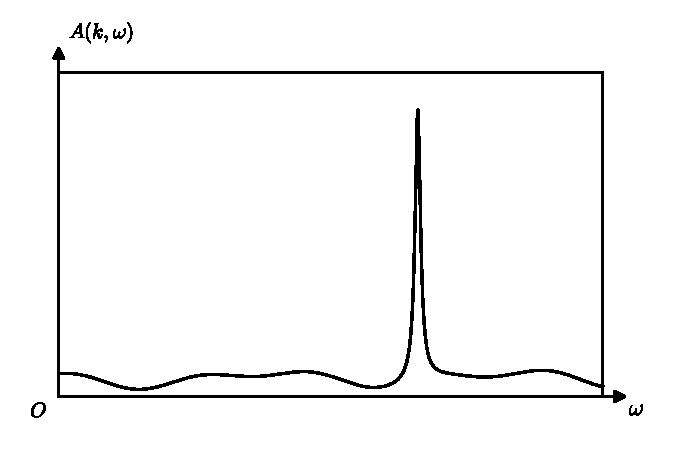
\includegraphics[width=9.5cm]{fig4-9.pdf}\\{\small 图 4.9\quad 谱函数示意图}
\end{minipage}
\end{center}

其中第二项
\begin{equation}
  g_{k}\equiv\int_{-\infty}^{\mu}A_{1}(k,\omega)\,\mathrm{d}\omega>0
\end{equation}
由于 $A_{1}$ 的正定性，其积分 $g_{k}$ 也应为正，又由于 $A_{1}$ 是 $\omega$ 的平滑函数，$g_{k}$ 也应为平滑函数，当 $k$ 越过费密面时，$g_{k}$ 应当是连续的，而式(4.11.36)右边第一项则是间断的
\begin{equation}
\begin{aligned}
  \widetilde{n}_{k}
  &=Z_{k}\int_{-\infty}^{\mu}
  \frac{\left(\varGamma_{k}/\pi\right)}
  {\left(\omega-\widetilde{E}_{k}\right)^{2}+\varGamma_{k}^{2}}\,\mathrm{d}\omega\\
  &=Z_{k}\int_{-\infty}^{\left(\mu-\widetilde{E}_{k}\right)/\varGamma_{k}}
  \frac{\mathrm{d}x}{1+x^{2}}\\
  &=Z_{k}\theta\left(\mu-\widetilde{E}_{k}\right)
  =\left\{\begin{array}{ll}
  Z_{k} & \left(\widetilde{E}_{k}<\mu\right)\\
  0 & \left(\widetilde{E}_{k}>\mu\right)
  \end{array}\right.
\end{aligned}
\end{equation}
其中利用了准粒子存在的条件 $|\widetilde{E}_{k}-\mu|\gg\varGamma_{k}$. 因此，当 $\widetilde{E}_{k}<\mu$ 时第二个等式中的积分上限可取为 $+\infty$，反之当 $\widetilde{E}_{k}>\mu$ 时取 $-\infty$，最后得到
\begin{equation}
  n_{k\sigma}=Z_{k}\theta\left(\mu-\widetilde{E}_{k}\right)+g_{k}
\end{equation}
显然，在越过费密面时准粒子的占据数有不连续的变化，其变化的大小为 $Z_{k}$，由于 $g_{k}$ 为正，而零温时 $n_{k\sigma}$ 的最大取值等于1，因此 $Z_{k}<1$. 图4.10中实线表示相互作用电子系统中占据数的动量分布示意曲线，而虚线则是熟知的零温费密分布
\begin{equation}
  n_{k\sigma}^{(0)}=\theta\left(\mu-E_{k}\right)=\theta\left(k_{\mathrm{F}}-k\right)
\end{equation}
代表自由电子的占据数分布，当越过 $k_{\mathrm{F}}$ 时，出现高度为1的台阶式间断，对应于无相互作用电子系统中存在明确的费密面.对于相互作用系统，这一明显的间断性依然存在，仅仅是间断值有所减小 $\left(Z_{k}<1\right)$，说明在 $k$ 空间仍然存在费密面.实验上，爱森伯格（Eisenberger）等人\textsuperscript{[20]}利用 X 射线的康普顿散射，在金属 Na 中已观察到占据数的明显间断，并证实了实际金属（带电）中确实存在费密面.

\begin{center}
\begin{minipage}{9.5cm}
\centering
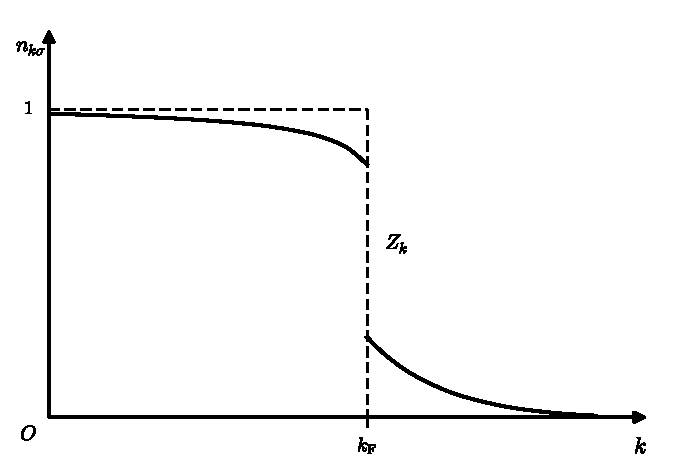
\includegraphics[width=9.5cm]{fig4-10.pdf}\\{\small 图4.10\quad 相互作用电子系中占据数的动量分布}
\end{minipage}
\end{center}

\begin{canKao}
\begin{enumerate}[label={[\arabic*]}, leftmargin=2.2em, itemsep=0pt]
\item 李正中. 相互作用费密系. 见: 蔡建华等编. 量子统计的格林函数理论. 北京: 科学出版社, 1983. 第4章
\item Nakajima S et al. The Physics of Elementary Excitation. New York: Springer-Verlag, 1980. Chap 3
\item Kubo R. J Phys Soc Japan, 1957, 12: 570
\item Fetter A L, Walecka J D. Quantum Theory of Many Particle System. New York: McGraw-Hill, 1971. Chap 4
\item Grimes C C et al. Phys Rev Lett, 1979, 42: 795
\item Halperin B I. Helv Phys Acta, 1983, 56: 75
\item Pines D. Solid State Phys, 1995, 1: 387
\item 孙鑫. 低维合作现象. 见: 郝柏林等编. 统计物理学进展. 北京: 科学出版社, 1981
\item Langer J S, Vosko S H. J Phys Chem Solids, 1960, 12: 196
\item Friedel J. Nuovo Cimento, 1958, 7 (suppl): 287
\item Gell-Mann M, Bruckner K A. Phys Rev, 1957, 106: 364
\item Hubbard J. Phys Rev, 1967, 25A: 709
\item Singwi K S et al. Phys Rev, 1970, B1: 1044
\item Wigner E. Trans Faraday Soc, 1938, 34: 678
\item Khurana A. Physics Today, 1990, 43: 17
\item Sholl C A. Proc Phys Soc (London), 1967, 92: 434
\item Nozieres P, Pines D. Phys Rev, 1958, 111: 442
\item Quinn J J, Ferrell R A. Phys Rev, 1958, 112: 812
\item Luttinger J M. Phys Rev, 1960, 119: 1153
\item Eisenberger P L et al. Phys Rev, 1972, B6: 3671
\end{enumerate}
\end{canKao}

% ============================================================
%  第五章 电子-声子相互作用（§1–§5 + 章末参考文献）
%  底本：高等教育出版社《固体理论》（第二版）印刷页 138–158
%  （PDF 页 = 印刷页 + 20，章名页 PDF p158，末页 PDF p178）
%  OCR 输入：MinerU/full_merged.md 行 6404–7197
%  公式编号自检：§1 (5.1.1)–(5.1.4)；§2 (5.2.1)–(5.2.31)；
%    §3 (5.3.1)–(5.3.20)；§4 (5.4.1)–(5.4.22)；§5 (5.5.1)–(5.5.20)。
%    共 97 个编号，全部自动编号，逐一对上原书。
%  缺号判定（对照原书页面）：任务单所示 3 处缺号均为 OCR 漏检而非原书跳号——
%    (5.2.16)：OCR 残 tag {2.16}，原书 p142 有此式，已补全；
%    (5.2.31)：N 过程跃迁概率大式 OCR 无 tag，原书 p145 有编号，已补排；
%    (5.4.10)：H_ep 一般式 OCR 乱码无 tag，原书 p149 有编号，已按原书重排；
%    (5.5.3) ：有效互作用矩阵元式 OCR 无 tag，原书 p154 有编号，已补排。
%    故本章实有编号公式 97 个（OCR tag 计数 94 ＋ 补排 3）。
%  已修正的 OCR/原书错误：
%  1. (5.1.4) 被拆成相邻两个 $$ 块（首行无号＋次行带号），按原书 p139
%     合并为一个编号公式
%  2. §1 "其中ε.是带边能量…"段 ε_c 重复串入、式(5.1.2)后杂符 $\pmb{c}_1$ 等，
%     按 p138 复原为"其中 ε_c 是……通常称为形变势，而 c_1 相应地称为……
%     式(5.1.2)就是电子-声子互作用的形变势模型[1]…"
%  3. (5.2.3) 第三行 V(r_i−l) 原书排印如此，按求和指标 j 与 ≡Σ_j h(r_j)
%     更正为 V(r_j−l)（原书排印错误）
%  4. (5.2.8) 第二行求和 Σ_{k,ν}→Σ_{k,k'}（OCR 误识，p141）
%  5. (5.2.10) (a_qs+q⁺_{−qs}) 原书排印如此，按 (5.2.9) 更正为
%     (a_qs+a⁺_{−qs})（原书排印错误）
%  6. (5.2.14) 末尾因子 e^{i(k−k')·l} OCR 漏失，按 p162 补
%  7. (5.2.16) OCR tag 残缺为 {2.16}、求和下标乱码（∑_{p'}、"(5.2.5),"串入），
%     按 p142 重排补全
%  8. §2 "分别代 e_qs 表 LA 与 TA 声子"→"分别代表 LA 与 TA 声子"（p143，
%     OCR 串入公式）；(ii) 段 X_n、k_n→K_n（OCR 误识＋原书小写排印）
%  9. §2 "总动量守恒条件相差hK，……所造 ħK_n 成的"按 p144 复原为
%     "相差 ħK_n，……所造成的"；"满足 j⃗格的动量守恒条件"按 p144 为
%     "满足严格的动量守恒条件"；"正格矢 a_i 0"补箭头 a_i→0
% 10. (5.2.27) 第二行箭头及条件 OCR 乱码，按 p145 为"(t 大时)⟹"；
%     (5.2.29) 的 S→δ；(5.2.28) ħω_{±q} 按原书
% 11. (5.2.31)：N 过程跃迁概率大式 OCR 无 tag 且排乱，原书 p145 有编号
%     (5.2.31)，已按原书重排补入；其下"(已占据态)(空占态)"处的 (n_k=1)
%     按 p145 补
% 12. §3 "这里晶体取单体积"→"单位体积"（p146）；(5.3.6)(5.3.7) 的 \frac{}{}
%     残缺按 p147 复原；(5.3.14) 相邻两块按原书（p147–148 跨页一式）合并；
%     (5.3.17) 整式 \textsf 乱码按 p148 重排
% 13. §4 (5.4.1) 首行 OCR 漏 e_q，按 p148 补为 e_q Q_q；(5.4.3) \sqrt{ΛM}→
%     \sqrt{NM}，W(r)=√(NM){u₊−u₋} 按 p149 复原
% 14. (5.4.10)：H_ep 一般式 OCR 严重乱码无 tag，原书 p149 有编号 (5.4.10)，
%     已按原书重排补入（C⁺_{k'} 的 k' 按 300dpi 页面核实）
% 15. §4 "−eφ(r) 代表处电子受 LO 声子…"按 p149 补"r"→"代表 r 处电子"；
%     "随 g 增大"→"随 q 增大"；"L0 声子"→"LO 声子"；"声子能量 hω1"→ħω_L；
%     OCR 串入的 ħω_L、Δt、α、q 等杂符已删（p151–152）
% 16. (5.4.19) 首行关系号按 p151 为 "≡"（OCR 作 =）
% 17. <N_ph>：OCR 乱码（\vec p\vec circ），按 p151 为 <N_声>（汉字下标"声"）
% 18. §4 "只有少数 Ⅱ-Ⅴ 族"按 p152 为"Ⅲ-Ⅴ族和 Ⅱ-Ⅵ族化合物半导体"；
%     表 5.1 的 MδgO→MgO、zns→ZnS、"5 InSb"→InSb
% 19. (5.5.2) 第二项分母 (ε_k−ε_{k+q}−ħω_{−q}) OCR 漏失，按 p153 补
% 20. (5.5.3)：有效互作用矩阵元式 OCR 无 tag，原书 p154 有编号 (5.5.3)，
%     已补排
% 21. §5 "|m_1|与图 5.7 中(a)对应"→|m_1⟩（OCR 键错）；"其中|n>Z|m>为 H_0
%     的本征态"→"|n>及|m>"（p156）
% 22. (5.5.16) 相邻两块按原书（p156–157 跨页一式）合并为一个编号公式；
%     (5.5.18) 分子 C_{kq}→C_{kσ}（p157）
% 23. §5 末段 "|ε_k−ε_{k+q}|<ħω_k" 原书排印如此，按同段能壳区条件更正为
%     ħω_q（原书排印错误）；ε_{k+q}、ω_q、ħω≡|ε_k−ε_{k+q}| 等乱码按
%     p157–158 复原；"由于晶格畸变以ω。频率响应电子(1)"→ω_q（OCR）
% 24. 文献[4][5] "Frohlich"按 p158 原书为"Fröhlich"，[4] 有 et al.
% 25. 其余：全角句点"．"→ASCII "."；OCR 间隔符 ~ 删除；\mathrm{d} 收紧；
%     \hat{δ}/\widehat{δ}→δ；\varrho→ρ；\epsilon 与 \varepsilon 统一为
%     \varepsilon；被拆散的"玻$n_q$色""决 定"等按原书合并
%  遗留问题：
%  · §1 "类似的，a_qC⁺_{k−q}C_k 也可以代表吸收声子后产生电子-空穴对"一句
%    原书即印作 C⁺_{k−q}（而图 5.2(b) 为 C⁺_{k+q}），两处照原书照录未改；
%  · §2 "将写出自旋为下一章讨论超导用"原书如此（无逗号），照录；
%  · 图 5.1–5.7 均为占位图（fig5-N.pdf），宽度按原书目测配置。
% ============================================================
\chapter{电子-声子相互作用}

\section{互作用过程}

能带论只计及了晶格周期势场对电子的作用.当考虑晶格振动时，由于原子（离子）偏离平衡位置会破坏周期场，引起势能的改变，将使能带电子受到晶格位移所产生附加势场的作用，这就是电子和晶格振动的相互作用.晶格振动由声子描述，因此这个互作用又称为电子与声子的相互作用.

在能带极值附近，波矢 $\boldsymbol{k}$ 和有效质量 $m$ 的电子能量可近似写为
\begin{equation}
  \varepsilon_k=\varepsilon_{\mathrm{c}}+\frac{\hbar^2k^2}{2m}
\end{equation}
其中 $\varepsilon_{\mathrm{c}}$ 是带边能量，可理解为能带电子的势能.如果不考虑晶格振动，则 $\varepsilon_{\mathrm{c}}$ 代表晶格周期势对电子的作用，它随晶格常数变化.由于格波的纵声学模（LA 声子）总是伴随着晶体体积和晶格常数的局域变化，因此存在晶格振动时，带边能量将发生移动
\begin{equation}
  \delta\varepsilon_{\mathrm{c}}=\left(\frac{\partial\varepsilon_{\mathrm{c}}}{\partial V}\right)\delta V
  =V\left(\frac{\partial\varepsilon_{\mathrm{c}}}{\partial V}\right)\left(\frac{\delta V}{V}\right)
  =c_1\Delta\left(\boldsymbol{r}\right)
\end{equation}
其中 $\Delta\left(\boldsymbol{r}\right)$ 是体积的相对变化，它反映晶格局域形变的大小，称为形变量.因此 $\delta\varepsilon_{\mathrm{c}}$ 代表晶格振动的形变所引起单电子势能的变化，通常称为形变势，而 $c_1$ 相应地称为形变势常数，其数值由实验确定.式(5.1.2)就是电子-声子互作用的形变势模型\textsuperscript{[1]}，广泛应用于金属和半导体问题.

在长波近似下，根据式(2.5.31)，可以用 LA 声子的产生算符 $a_q^{+}$ 与消灭算符 $a_q$ 表示 $\Delta\left(\boldsymbol{r}\right)$，即
\begin{equation}
  \Delta\left(\boldsymbol{r}\right)=\nabla\cdot\boldsymbol{u}\left(\boldsymbol{r}\right)
  =\mathrm{i}\sum_{q}\sqrt{\frac{\hbar}{2\rho V\omega_q}}
  \left(\boldsymbol{e}_q\cdot\boldsymbol{q}\right)
  \left(a_q\mathrm{e}^{\mathrm{i}\boldsymbol{q}\cdot\boldsymbol{r}}
  -a_q^{+}\mathrm{e}^{-\mathrm{i}\boldsymbol{q}\cdot\boldsymbol{r}}\right)
\end{equation}
电子-声子互作用的二次量子化表示式由单体势 $\delta\varepsilon_{\mathrm{c}}$ 对态向量的平均决定，即
\begin{equation}
\begin{aligned}
  H_{\mathrm{ep}}&=\int\mathrm{d}\boldsymbol{r}\,\varPsi^{+}\left(\boldsymbol{r}\right)
  c_1\Delta\left(\boldsymbol{r}\right)\varPsi\left(\boldsymbol{r}\right)\\
  &=\mathrm{i}c_1\sum_{k,q}\sqrt{\frac{\hbar}{2\rho V\omega_q}}
  \left(\boldsymbol{e}_q\cdot\boldsymbol{q}\right)
  \left(a_qC_{k+q}^{+}C_k-a_q^{+}C_{k-q}^{+}C_k\right)
\end{aligned}
\end{equation}
式(5.1.4)给出电子-声子互作用的两个基本过程：(a)$\boldsymbol{k}$ 电子吸收 $\boldsymbol{q}$ 声子变为 $\boldsymbol{k}+\boldsymbol{q}$ 态上的电子；(b)$\boldsymbol{k}$ 电子发射 $\boldsymbol{q}$ 声子变为 $\boldsymbol{k}-\boldsymbol{q}$ 态上的电子.用二次量子化术语说：$a_qC_{k+q}^{+}C_k$ 为消灭 $\boldsymbol{k}$ 电子和 $\boldsymbol{q}$ 声子并产生 $\boldsymbol{k}+\boldsymbol{q}$ 电子，如图5.1(a)所示.$a_q^{+}C_{k-q}^{+}C_k$ 则代表 $\boldsymbol{k}$ 电子被消灭和 $\boldsymbol{q}$ 声子与 $\boldsymbol{k}-\boldsymbol{q}$ 电子产生，由图5.1(b)表示.

\begin{center}
\begin{minipage}{7.5cm}
\centering
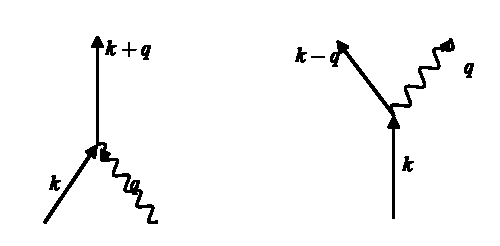
\includegraphics[width=7.5cm]{fig5-1.pdf}\\[0.3em]
{\small (a) $a_qC_{k+q}^{+}C_k$ 声子吸收\qquad\qquad (b) $a_q^{+}C_{k-q}^{+}C_k$ 声子发射}\\[0.2em]
{\small 图 5.1\quad 电子-声子互作用的一级过程}
\end{minipage}
\end{center}

当 $\boldsymbol{k}$ 在费密球外而 $\boldsymbol{k}-\boldsymbol{q}$ 在费密球内时，$a_q^{+}C_{k-q}^{+}C_k$ 将代表消灭 $\boldsymbol{k}$ 电子和 $\boldsymbol{k}-\boldsymbol{q}$ 空穴，并产生 $\boldsymbol{q}$ 声子，即常见的电子-空穴对复合发射声子的过程.类似的，$a_qC_{k-q}^{+}C_k$ 也可以代表吸收声子后产生电子-空穴对.在图5.2中箭头朝上代表电子，箭头朝下代表空穴.

\begin{center}
\begin{minipage}{8cm}
\centering
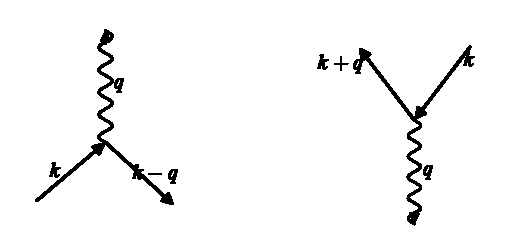
\includegraphics[width=8cm]{fig5-2.pdf}\\[0.3em]
{\small (a) $a_q^{+}C_{k-q}^{+}C_k$ 电子-空穴对复合发射声子\qquad (b) $a_qC_{k+q}^{+}C_k$ 吸收声子产生电子-空穴对}\\[0.2em]
{\small 图 5.2\quad 电子-空穴对的产生与复合}
\end{minipage}
\end{center}

以上是 $H_{\mathrm{ep}}$ 的一级微扰过程，它用于解释晶体的输运特性，如电阻的成因等.电子-声子互作用的高阶微扰过程由上述基本过程组成，例如二级微扰的下列3个图形［图5.3(a)、(b)、(c)］.图形(a)为电子在运动时先发射后吸收 $\boldsymbol{q}$ 声子，物理实质是电子带着晶格畸变运动，这必然会对电子自身的能量产生修正，称为电子自能修正图.图形(b)代表声子自能修正，因为电子系统对声子扰动场的屏蔽，将改变离子间的互作用势，从而对声子频率产生修正.图形(c)则是两个电子通过声子的间接互作用，在一定条件下将成为电子之间的有效吸引势，它是产生超导电性的主要机制.在§3—§5中我们将结合具体问题讨论这3个二级过程.

\begin{center}
\begin{minipage}{10.5cm}
\centering
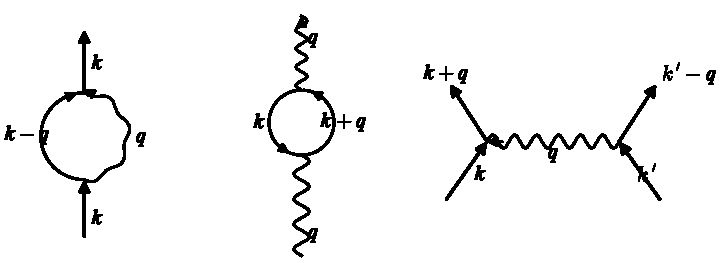
\includegraphics[width=10.5cm]{fig5-3.pdf}\\[0.3em]
{\small (a) 电子自能修正\qquad (b) 声子自能修正\qquad (c) 电子-声子-电子互作用}\\[0.2em]
{\small 图 5.3\quad 二级过程}
\end{minipage}
\end{center}

\section{电子与声频支声子的相互作用}

以上是电子与声子互作用的连续模型，而更严格的推导应当从晶格模型出发\textsuperscript{[2]}.对于简单晶格只有声频支振动，电子与晶格振动的相互作用就是电子与声频声子的互作用.设 $\boldsymbol{l}$ 格点上离子与 $j$ 电子（位置由 $\boldsymbol{r}_j$ 表示）之间的相互作用势能为 $V\left(\boldsymbol{r}_j-\boldsymbol{l}\right)$，则当离子不动时电子与离子的互作用为
\begin{equation}
  H_{\mathrm{ei}}^{0}=\sum_{j,l}V\left(\boldsymbol{r}_j-\boldsymbol{l}\right)
\end{equation}
它表示电子在周期场中的势能，这里 $\boldsymbol{l}\equiv\boldsymbol{R}_l=\sum_{i}l_i\boldsymbol{a}_i$.实际上离子在不断地振动，其相对位移为 $\boldsymbol{u}_l\left(t\right)$，电子与离子互作用应当是
\begin{equation}
  H_{\mathrm{ei}}=\sum_{j,l}V\left(\boldsymbol{r}_j-\boldsymbol{l}-\boldsymbol{u}_l\right)
\end{equation}
因此，能带电子与晶格振动的相互作用由式(5.2.2)与式(5.2.1)之差表示
\begin{equation}
\begin{aligned}
  H_{\mathrm{ep}}&=H_{\mathrm{ei}}-H_{\mathrm{ei}}^{0}\\
  &=\sum_{j,l}\left\{V\left(\boldsymbol{r}_j-\boldsymbol{l}-\boldsymbol{u}_l\right)
  -V\left(\boldsymbol{r}_j-\boldsymbol{l}\right)\right\}\\
  &=-\sum_{j,l}\boldsymbol{u}_l\cdot\nabla V\left(\boldsymbol{r}_j-\boldsymbol{l}\right)
  \equiv\sum_{j}h\left(\boldsymbol{r}_j\right)
\end{aligned}
\end{equation}
其中电子与声子互作用的单体势为
\begin{equation}
  h\left(\boldsymbol{r}\right)=-\sum_{l}\boldsymbol{u}_l\cdot\nabla V\left(\boldsymbol{r}-\boldsymbol{l}\right)
\end{equation}
若选布洛赫函数
\begin{equation}
  \psi_k\left(\boldsymbol{r}\right)=u_k\left(\boldsymbol{r}\right)\mathrm{e}^{\mathrm{i}\boldsymbol{k}\cdot\boldsymbol{r}}
  \text{，}\quad u_k\left(\boldsymbol{r}+\boldsymbol{l}\right)=u_k\left(\boldsymbol{r}\right)
\end{equation}
作为电子系统二次量子化态向量的基函数，则
\begin{equation}
  \varPsi\left(\boldsymbol{r}\right)=\sum_{k}C_k\psi_k\left(\boldsymbol{r}\right)
  \text{，}\quad \varPsi^{+}\left(\boldsymbol{r}\right)=\sum_{k}C_k^{+}\psi_k^{+}\left(\boldsymbol{r}\right)
\end{equation}
式中 $C_k^{+}$ 和 $C_k$ 为能带电子的产生及消灭算符，满足费密子的反对易关系
\begin{equation}
  \left[\,C_k,C_{k'}^{+}\,\right]_{+}=\delta_{kk'}\text{，}
  \left[\,C_k,C_{k'}\,\right]_{+}=\left[\,C_k^{+},C_{k'}^{+}\,\right]_{+}=0
\end{equation}
为了记号简单起见在这里暂不标明自旋指标 $\sigma$，只需注意对 $\boldsymbol{k}$ 求和应包括自旋简并度.在§5中讨论电子间有效吸引互作用时，将写出自旋为下一章讨论超导用.

从单体势容易求出用电子算符表示的电子-声子互作用为：
\begin{equation}
\begin{aligned}
  H_{\mathrm{ep}}&=\int\varPsi^{+}\left(\boldsymbol{r}\right)h\left(\boldsymbol{r}\right)\varPsi\left(\boldsymbol{r}\right)\mathrm{d}\boldsymbol{r}\\
  &=\sum_{k,k'}\left\langle k'\left|h\left(\boldsymbol{r}\right)\right|k\right\rangle C_{k'}^{+}C_k\\
  &=-\sum_{l}\sum_{k,k'}\boldsymbol{u}_l\cdot\left\langle k'\left|\nabla V\left(\boldsymbol{r}-\boldsymbol{l}\right)\right|k\right\rangle C_{k'}^{+}C_k
\end{aligned}
\end{equation}
再将晶格振动用声子算符表示
\begin{equation}
  \left.\begin{aligned}
  \boldsymbol{u}_l&=\frac{1}{\sqrt{NM}}\sum_{q,s}\boldsymbol{e}_{qs}Q_{qs}\mathrm{e}^{\mathrm{i}\boldsymbol{q}\cdot\boldsymbol{l}}\\
  Q_{qs}&=\sqrt{\frac{\hbar}{2\omega_{qs}}}\left(a_{qs}+a_{-qs}^{+}\right)\\
  \boldsymbol{e}_{qs}&=\boldsymbol{e}_{-qs}\text{，}\ \left|\boldsymbol{e}_{qs}\right|=1
  \end{aligned}\right\}
\end{equation}
代入式(5.2.8)，求得 $H_{\mathrm{ep}}$ 的二次量子化表示
\begin{equation}
\begin{aligned}
  H_{\mathrm{ep}}&=-\sum_{l}\sum_{k,k'}\sum_{q,s}\left(\frac{\hbar}{2NM\omega_{qs}}\right)^{1/2}
  \left(a_{qs}+a_{-qs}^{+}\right)C_{k'}^{+}C_k\mathrm{e}^{\mathrm{i}\boldsymbol{q}\cdot\boldsymbol{l}}\times\\
  &\quad\left\{\boldsymbol{e}_{qs}\cdot\left\langle k'\left|\nabla V\left(\boldsymbol{r}-\boldsymbol{l}\right)\right|k\right\rangle\right\}
\end{aligned}
\end{equation}
其中 $N$ 为元胞数，$M$ 为离子质量，$s$ 代表格波的偏振指标.布洛赫函数的积分
\begin{equation}
  \left\langle k'\left|\nabla V\left(\boldsymbol{r}-\boldsymbol{l}\right)\right|k\right\rangle
  =\int\mathrm{d}\boldsymbol{r}\,u_{k'}^{*}\left(\boldsymbol{r}\right)u_k\left(\boldsymbol{r}\right)
  \mathrm{e}^{\mathrm{i}\left(\boldsymbol{k}-\boldsymbol{k}'\right)\cdot\boldsymbol{r}}\nabla V\left(\boldsymbol{r}-\boldsymbol{l}\right)
\end{equation}
由于晶体满足周期性边界条件，作 $\boldsymbol{r}\to\boldsymbol{r}+\boldsymbol{l}$ 代换积分不变，再利用 $\boldsymbol{u}_k\left(\boldsymbol{r}+\boldsymbol{l}\right)=\boldsymbol{u}_k\left(\boldsymbol{r}\right)$，可将上式简化为
\begin{equation}
\begin{aligned}
  &\left\langle k'\left|\nabla V\left(\boldsymbol{r}-\boldsymbol{l}\right)\right|k\right\rangle\\
  &=\left\{\int\mathrm{d}\boldsymbol{r}\,u_{k'}^{*}\left(\boldsymbol{r}\right)u_k\left(\boldsymbol{r}\right)
  \mathrm{e}^{\mathrm{i}\left(\boldsymbol{k}-\boldsymbol{k}'\right)\cdot\boldsymbol{r}}\nabla V\left(\boldsymbol{r}\right)\right\}
  \mathrm{e}^{\mathrm{i}\left(\boldsymbol{k}-\boldsymbol{k}'\right)\cdot\boldsymbol{l}}
\end{aligned}
\end{equation}
对离子势作傅里叶展开
\begin{equation}
  V\left(\boldsymbol{r}\right)=\sum_{p}V_p\mathrm{e}^{\mathrm{i}\boldsymbol{p}\cdot\boldsymbol{r}}
\end{equation}
可求得
\begin{equation}
  \left\langle k'\left|\nabla V\left(\boldsymbol{r}-\boldsymbol{l}\right)\right|k\right\rangle
  =\mathrm{i}\sum_{p}\boldsymbol{p}V_p\left\langle k'\left|\mathrm{e}^{\mathrm{i}\boldsymbol{p}\cdot\boldsymbol{r}}\right|k\right\rangle
  \mathrm{e}^{\mathrm{i}\left(\boldsymbol{k}-\boldsymbol{k}'\right)\cdot\boldsymbol{l}}
\end{equation}
其中
\begin{equation}
  \left\langle k'\left|\mathrm{e}^{\mathrm{i}\boldsymbol{p}\cdot\boldsymbol{r}}\right|k\right\rangle
  =\int\mathrm{d}\boldsymbol{r}\,u_{k'}^{*}\left(\boldsymbol{r}\right)u_k\left(\boldsymbol{r}\right)
  \mathrm{e}^{\mathrm{i}\left(\boldsymbol{k}+\boldsymbol{p}-\boldsymbol{k}'\right)\cdot\boldsymbol{r}}
\end{equation}
将式(5.2.14)代入式(5.2.10)
\begin{equation}
\begin{aligned}
  H_{\mathrm{ep}}&=-\mathrm{i}\sum_{k,k'}\sum_{q,s}\sum_{p}\left(\frac{N\hbar}{2M\omega_{qs}}\right)^{1/2}
  \left(\boldsymbol{e}_{qs}\cdot\boldsymbol{p}\right)
  \left\{\frac{1}{N}\sum_{l}\mathrm{e}^{\mathrm{i}\left(\boldsymbol{k}+\boldsymbol{q}-\boldsymbol{k}'\right)\cdot\boldsymbol{l}}\right\}\times\\
  &\quad V_p\left\langle k'\left|\mathrm{e}^{\mathrm{i}\boldsymbol{p}\cdot\boldsymbol{r}}\right|k\right\rangle
  \left(a_{qs}+a_{-qs}^{+}\right)C_{k'}^{+}C_k
\end{aligned}
\end{equation}
为简单起见，用平面波代替布洛赫函数，取
\begin{equation}
  u_k\left(\boldsymbol{r}\right)=\left(N\Omega\right)^{-1/2}
\end{equation}
得到
\begin{equation}
  \left\langle k'\left|\mathrm{e}^{\mathrm{i}\boldsymbol{p}\cdot\boldsymbol{r}}\right|k\right\rangle
  =\frac{1}{N\Omega}\int\mathrm{e}^{\mathrm{i}\left(\boldsymbol{k}+\boldsymbol{p}-\boldsymbol{k}'\right)\cdot\boldsymbol{r}}\mathrm{d}\boldsymbol{r}
  =\delta_{p,\,k'-k}
\end{equation}
再利用求和关系
\begin{equation}
  \frac{1}{N}\sum_{l}\mathrm{e}^{\mathrm{i}\left(\boldsymbol{k}+\boldsymbol{q}-\boldsymbol{k}'\right)\cdot\boldsymbol{l}}
  =\delta_{k',\,k+q+\boldsymbol{K}_n}
\end{equation}
和波矢条件
\begin{equation}
  \boldsymbol{p}=\boldsymbol{k}'-\boldsymbol{k}=\boldsymbol{q}+\boldsymbol{K}_n
\end{equation}
其中 $\boldsymbol{K}_n=\sum_{i=1}^{3}n_i\boldsymbol{b}_i$ 为任意倒格矢，$n_i$ 取整数.这样就得到晶格模型中电子与声子互作用的哈密顿量.
\begin{equation}
\begin{aligned}
  H_{\mathrm{ep}}&=-\mathrm{i}\sum_{k}\sum_{q,s}\left(\frac{N\hbar}{2M\omega_{qs}}\right)^{1/2}
  V_{q+\boldsymbol{K}_n}\left\{\boldsymbol{e}_{qs}\cdot\left(\boldsymbol{q}+\boldsymbol{K}_n\right)\right\}\times\\
  &\quad\left(a_{qs}+a_{-qs}^{+}\right)C_{k+q+\boldsymbol{K}_n}^{+}C_k
\end{aligned}
\end{equation}
剩下的问题是如何选取倒格矢 $\boldsymbol{K}_n$.当采用简约区方案时，$\boldsymbol{q}$，$\boldsymbol{k}$ 与 $\boldsymbol{k}'$ 都是简约波矢，应同时位于第一布里渊区之内，由于 $\boldsymbol{k}+\boldsymbol{q}$ 可能超出第一布里渊区，因此 $\boldsymbol{K}_n$ 的选取应保证散射后的电子态 $\boldsymbol{k}'=\boldsymbol{k}+\boldsymbol{q}+\boldsymbol{K}_n$ 也在第一布里渊区内.现在分下列两种情况讨论：

\subsection*{(i) $\boldsymbol{k}+\boldsymbol{q}$ 在第一布里渊区之内}

取 $\boldsymbol{K}_n=0$，这时 $\boldsymbol{k}'=\boldsymbol{k}+\boldsymbol{q}$，总波矢守恒，称为正常散射过程或简称 N 过程.由于在长波近似下有 $\boldsymbol{e}_{qs}$ 平行或垂直于波矢 $\boldsymbol{q}$ 的解，分别代表 LA 与 TA 声子.显然，对于 N 过程 $H_{\mathrm{ep}}$ 中只有 LA 声子的贡献.
\begin{equation}
  H_{\mathrm{ep}}=\sum_{k,q}D_q\left(a_q+a_{-q}^{+}\right)C_{k+q}^{+}C_k
\end{equation}
其中
\begin{equation}
  D_q\equiv-\mathrm{i}\left(\frac{N\hbar}{2M\omega_q}\right)^{1/2}V_q
  \left(\boldsymbol{e}_q\cdot\boldsymbol{q}\right)
\end{equation}
$\omega_q$ 与 $\boldsymbol{e}_q$ 代表 LA 声子的频率和极化矢量.

当讨论金属中电子与声子互作用问题时，往往采用集体坐标表示 $H_{\mathrm{ep}}$.设金属为单价，电子与离子间互作用取库仑势，则 $V_q=-\dfrac{4\pi e^2}{q^2}$.这时，根据式(2.5.29)引入声子简正坐标 $Q_q$ 和电子集体坐标 $\rho_{-q}=\sum\limits_{k}C_{k+q}^{+}C_k$，可将式(5.2.22)写成
\begin{equation}
  H_{\mathrm{ep}}=\sum_{q}M_qQ_q\rho_{-q}\text{，}\ M_q=\mathrm{i}\left(\frac{N}{M}\right)^{1/2}
  \frac{4\pi e^2}{q^2}\left(\boldsymbol{e}_q\cdot\boldsymbol{q}\right)
\end{equation}
这是电子-声子互作用哈密顿量的集体坐标表示式，用于自洽计算金属电子气对声子频率修正等具体问题.

\subsection*{(ii) $\boldsymbol{k}+\boldsymbol{q}$ 超出第一布里渊区}

取 $\boldsymbol{K}_n\neq 0$，所取 $\boldsymbol{K}_n$ 应使 $\boldsymbol{k}+\boldsymbol{q}+\boldsymbol{K}_n$ 回到第一布里渊区之内，描述散射后的电子态 $\boldsymbol{k}'$.这时总波矢守恒条件相差一个倒格矢，由 $\boldsymbol{k}'=\boldsymbol{k}+\boldsymbol{q}+\boldsymbol{K}_n$ 表示.由于 $\boldsymbol{k}$ 与 $\boldsymbol{q}$ 均限于第一布里渊区内，故 $\boldsymbol{k}+\boldsymbol{q}$ 一般只落在邻近布里渊区中，如图5.4所示.$\boldsymbol{K}_n\neq 0$ 时在 $H_{\mathrm{ep}}$ 的表示式(5.2.21)中有 $\left\{\boldsymbol{e}_{qs}\cdot\left(\boldsymbol{q}+\boldsymbol{K}_n\right)\right\}$ 因子存在，尽管横波的 $\boldsymbol{e}_{q\mathrm{T}}\cdot\boldsymbol{q}=0$，但因 $\boldsymbol{e}_{q\mathrm{T}}\cdot\boldsymbol{K}_n\neq 0$，这时 LA 与 TA 声子都对互作用有贡献.

由图5.4可知，从 $\boldsymbol{k}$ 到 $\boldsymbol{k}'$ 为大角度散射.这不是由于采用简约区方案造成的.

\begin{center}
\begin{minipage}{7cm}
\centering
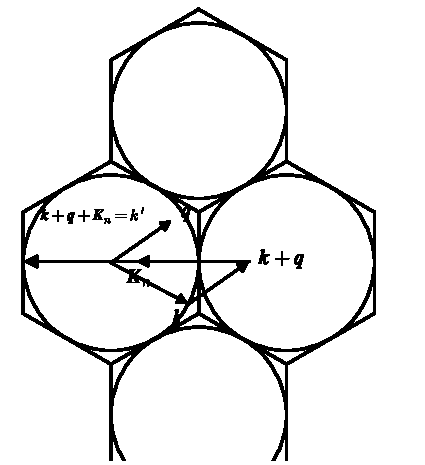
\includegraphics[width=7cm]{fig5-4.pdf}\\{\small 图 5.4\quad U 过程}
\end{minipage}
\end{center}

实际上在 BZ 之外，$\boldsymbol{k}+\boldsymbol{q}$ 处电子的速度与简约区内 $\boldsymbol{k}'=\boldsymbol{k}+\boldsymbol{q}+\boldsymbol{K}_n$ 点电子速度相同，它们都垂直于图中绘出的球形等能面.比较 $\boldsymbol{v}\left(\boldsymbol{k}\right)$ 和 $\boldsymbol{v}\left(\boldsymbol{k}+\boldsymbol{q}\right)$ 或 $\boldsymbol{v}\left(\boldsymbol{k}+\boldsymbol{q}+\boldsymbol{K}_n\right)$，显然散射前后电子速度发生了大角度偏转，好像经过了翻转，故常称 $\boldsymbol{K}_n\neq 0$ 的过程为 U 过程或倒逆过程.图5.5是 U 过程散射前后能带电子速度的变化，其中 $\boldsymbol{k}'=\boldsymbol{k}+\boldsymbol{q}+\boldsymbol{K}_n$ 代表散射后电子的简约波矢，而 $\boldsymbol{k}+\boldsymbol{q}$ 为不采用简约区方案时的散射波矢.由于在两种情况下速度相同，说明采用简约区方案划分 N 与 U 过程并不改变物理实质，仅仅是为了处理问题方便.

\begin{center}
\begin{minipage}{7.5cm}
\centering
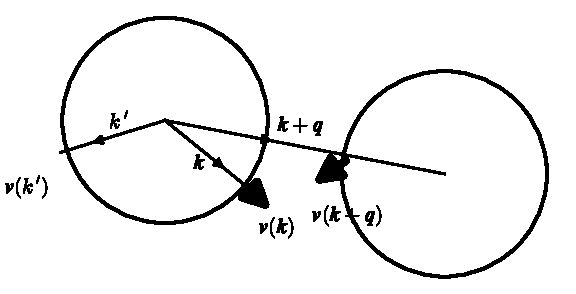
\includegraphics[width=7.5cm]{fig5-5.pdf}\\{\small 图 5.5\quad U 过程散射的电子速度图}
\end{minipage}
\end{center}

U 过程对于金属的高温特性有重要影响，因为在高温时大 $\boldsymbol{q}$ 值的散射过程增多，这时 $\boldsymbol{k}+\boldsymbol{q}$ 超出第一布里渊区的机会也多，于是 U 过程出现的概率增大.在低温下，当长波近似适用时，主要是 N 过程.

现在讨论电子-声子互作用过程的守恒律.由于 $H_{\mathrm{ep}}$ 只含声子产生及消灭算符的一次项，因此每次相互作用电子只可能吸收或发射一个声子.根据式(5.2.20)电子与声子的散射过程满足准动量关系
\begin{equation}
  \hbar\boldsymbol{k}'=\hbar\left(\boldsymbol{k}+\boldsymbol{q}+\boldsymbol{K}_n\right)
\end{equation}
显然，总动量守恒条件相差 $\hbar\boldsymbol{K}_n$，这是晶体结构的周期性和不连续性所造成的.假如完全忽略晶体的结构，则晶格求和 $\frac{1}{N}\sum\limits_{l}\mathrm{e}^{\mathrm{i}\left(\boldsymbol{k}+\boldsymbol{q}-\boldsymbol{k}'\right)\cdot\boldsymbol{l}}$ 过渡为连续积分
\begin{equation}
  \left(\frac{1}{N\Omega}\right)\int\mathrm{d}\boldsymbol{r}\;
  \mathrm{e}^{\mathrm{i}\left(\boldsymbol{k}+\boldsymbol{q}-\boldsymbol{k}'\right)\cdot\boldsymbol{r}}
  =\delta_{k',\,k+q}
\end{equation}
满足严格的动量守恒条件.这相当于假定晶体对无限小位移具有平移不变性，即正格矢 $\boldsymbol{a}_i\to 0$ 时，倒格矢 $\boldsymbol{b}_i\to\infty$，第一布里渊区变为无限大，也就不存在 $\boldsymbol{k}+\boldsymbol{q}$ 超出 BZ 的问题了.所以，一旦计及了晶体结构的影响，就会出现差 $\hbar\boldsymbol{K}_n$ 的准动量守恒条件，这是固体中元激发的特征.

讨论电子-声子散射过程的能量关系时，要区分实过程（可观测的）与虚过程（不可观测的）.先讨论实过程，根据含时微扰理论，从电子-声子系统的初态 $\left|i\right\rangle$ 到终态 $\left|f\right\rangle$ 的跃迁概率为
\begin{equation}
\begin{aligned}
  W\left(i\to f\right)&=\frac{2\pi}{\hbar}\left|\left\langle f\middle|H_{\mathrm{ep}}\middle|i\right\rangle\right|^2
  \frac{\sin^{2}\left(\dfrac{E_f-E_i}{2\hbar}\right)t}{\pi\left(\dfrac{t}{2\hbar}\right)\left(E_f-E_i\right)^2}\\
  &\overset{(t\ \text{大时})}{\Longrightarrow}\ \frac{2\pi}{\hbar}
  \left|\left\langle f\middle|H_{\mathrm{ep}}\middle|i\right\rangle\right|^2\delta\left(E_f-E_i\right)
\end{aligned}
\end{equation}
其中
\begin{equation}
  E_f-E_i=\varepsilon_{k'}-\varepsilon_k\mp\hbar\omega_{\pm q}
  \text{，}\quad \boldsymbol{k}'=\boldsymbol{k}+\boldsymbol{q}+\boldsymbol{K}_n
\end{equation}
若把电子与声子看作两个相互作用的子系统，则只有当我们能够确定电子从初态到终态的能量变化 $\Delta E=\left|\varepsilon_k-\varepsilon_{k'}\right|$ 时，这一跃迁才是可能的.按照不确定关系，这时应要求 $t\gg\hbar/\Delta E$ 才能将式(5.2.27)写成 $\delta$ 函数.又因为对于电子-声子散射过程，$t$ 最长只能取发生两次相继散射的平均间隔时间 $\tau$（弛豫时间），即 $t\leqslant\tau$.由此可知，只有当电子-声子散射的弛豫时间满足条件
\begin{equation*}
  \tau\gg\frac{\hbar}{\Delta E}\text{，}\qquad \Delta E=\left|\varepsilon_k-\varepsilon_{k+q}\right|
\end{equation*}
时才能得到
\begin{equation}
  W\left(i\to f\right)=\frac{2\pi}{\hbar}\left|\left\langle f\middle|H_{\mathrm{ep}}\middle|i\right\rangle\right|^2
  \delta\left(E_f-E_i\right)
\end{equation}
上式说明散射前后总能量守恒.参考式(5.2.28)，能量守恒条件为
\begin{equation}
  \varepsilon_{k'}=\varepsilon_{k+q}=\varepsilon_k\pm\hbar\omega_{\pm q}=\varepsilon_k\pm\hbar\omega_q
\end{equation}
式(5.2.30)对于 N 过程和 U 过程都一样，因为当电子在同一能带中发生跃迁时，$\varepsilon_{k+q}=\varepsilon_{k+q+\boldsymbol{K}_n}=\varepsilon_{k'}$.此外，在式(5.2.30)中还应用了时间反演对称性 $\omega_{-q}=\omega_q$.

由此不难求得电子从 $\boldsymbol{k}$ 态到 $\boldsymbol{k}+\boldsymbol{q}$ 的 N 过程跃迁概率为
\begin{equation}
\begin{aligned}
  W\left(\boldsymbol{k}\to\boldsymbol{k}+\boldsymbol{q}\right)&=\frac{2\pi}{\hbar}\left|D_q\right|^2
  \bigl\{\delta\left(\varepsilon_{k+q}-\varepsilon_k-\hbar\omega_q\right)\times\\
  &\quad\left|\left\langle n_{k+q}+1,n_k-1;n_q-1,n_{-q}\middle|a_qC_{k+q}^{+}C_k
  \middle|n_{k+q},n_k;n_q,n_{-q}\right\rangle\right|^2+\\
  &\quad\delta\left(\varepsilon_{k+q}-\varepsilon_k+\hbar\omega_q\right)\times\\
  &\quad\left|\left\langle n_{k+q}+1,n_k-1;n_q,n_{-q}+1\middle|a_{-q}^{+}C_{k+q}^{+}C_k
  \middle|n_{k+q},n_k;n_q,n_{-q}\right\rangle\right|^2\bigl\}\\
  &=\frac{2\pi}{\hbar}\left|D_q\right|^2\left(1-n_{k+q}\right)n_k
  \bigl\{n_q\delta\left(\varepsilon_{k+q}-\varepsilon_k-\hbar\omega_q\right)+\\
  &\quad\left(n_{-q}+1\right)\delta\left(\varepsilon_{k+q}-\varepsilon_k+\hbar\omega_q\right)\bigr\}
\end{aligned}
\end{equation}
以上结果仅仅涉及电子从已占据态 $\left(n_k=1\right)$ 向空占态 $\left(n_{k+q}=0\right)$ 的跃迁，因此在第一个等号右边的状态中，$\left(n_{k+q}+1\right)$ 与 $\left(n_k-1\right)$ 实际上分别为 1 与 0 占据，符合电子系统的泡利原理，而第二个等号右边的因子 $\left(1-n_{k+q}\right)n_k$ 在此情形下实际上等于 1.在这里保留该因子的目的是为了将以上结果推广用于 $T>0$ 情形，这时只需将 $n_k$ 与 $n_q$ 等分别用费密与玻色分布代替，即可将上式推广用于计算有限温度时电子与声子散射的弛豫时间，给出正确的电阻温度关系.

\section{声子的自能修正}

现在利用电子与声子互作用的集体坐标表示式(5.2.24)计算 LA 声子的自能修正.考虑单价金属，设 $N$ 个离子组成的简单晶格浸没在均匀电子气体中.与电子集体振荡相类似，在此模型中未微扰的 LA 声子频率在长波范围内可用离子的等离子集体振荡频率表示
\begin{equation}
  \Omega_q^2=\frac{4\pi Ne^2}{M}
\end{equation}
这里晶体取单位体积，$N=\Omega^{-1}$，$\Omega$ 为正点阵元胞体积.将上式代入式(2.4.3)，得到 LA 声子的哈密顿量
\begin{equation}
  H_{\mathrm{p}}=\frac{1}{2}\sum_{q}\left\{P_{-q}P_q+\Omega_q^2Q_{-q}Q_q\right\}
\end{equation}
其中 $P_{-q}=\dot{Q}_q$.电子与声子互作用为
\begin{equation*}
  H_{\mathrm{ep}}=\sum_{q}M_qQ_q\rho_{-q}
\end{equation*}
金属的总哈密顿量
\begin{equation}
  H=H_{\mathrm{p}}+H_{\mathrm{ep}}+H_{\mathrm{e}}+H_{\mathrm{ee}}
\end{equation}
其中 $H_{\mathrm{e}}$ 为自由电子近似的哈密顿量，$H_{\mathrm{ee}}$ 代表电子之间的库仑互作用，这两项均与声子的简正坐标 $Q_q$ 无关.

根据海森伯方程 $\mathrm{i}\hbar\dot{P}_{-q}=\left[P_{-q},H\right]$ 和对易式 $\left[P_q,Q_{q'}\right]=\dfrac{\hbar}{\mathrm{i}}\delta_{qq'}$，立刻可导出 $Q_q$ 的运动方程
\begin{equation}
  \ddot{Q}_q+\Omega_q^2Q_q=-M_{-q}\rho_q
\end{equation}
其中
\begin{equation}
  M_{-q}=-\mathrm{i}\left(\frac{N}{M}\right)^{1/2}\frac{4\pi e^2}{q^2}
  \left(\boldsymbol{e}_q\cdot\boldsymbol{q}\right)
\end{equation}
如果能确定式(5.3.4)右边的 $\rho_q$ 与 $Q_q$ 之间的关系，则声子频率的修正就可以求出.

由于晶格振动必然产生离子密度的起伏，可用离子密度的傅里叶分量 $\rho_q^{\mathrm{i}}$ 描述.这个起伏的效果相当于对电子气体加上外扰动场，它将引起电子气体的响应运动，从而使均匀分布的电子气产生密度起伏 $\rho_q$.所以，首先应找出 $\rho_q^{\mathrm{i}}$ 与简正坐标的关系，然后再利用线性响应理论决定 $\rho_q$ 与 $\rho_q^{\mathrm{i}}$ 的关系.

\subsection*{(i) 离子密度起伏 $\rho_q^{\mathrm{i}}$}

晶格振动位移将产生极化
\begin{equation}
\begin{aligned}
  \boldsymbol{P}\left(\boldsymbol{r}\right)&=Ne\,\boldsymbol{u}\left(\boldsymbol{r}\right)\\
  \boldsymbol{u}\left(\boldsymbol{r}\right)&=\left(NM\right)^{-1/2}\sum_{q}\boldsymbol{e}_qQ_q\mathrm{e}^{\mathrm{i}\boldsymbol{q}\cdot\boldsymbol{r}}
\end{aligned}
\end{equation}
由极化可得到离子密度
\begin{equation}
  \rho^{\mathrm{i}}\left(\boldsymbol{r}\right)=-\frac{1}{e}\nabla\cdot\boldsymbol{P}\left(\boldsymbol{r}\right)
  =-\mathrm{i}\left(\frac{N}{M}\right)^{1/2}\sum_{q}\left(\boldsymbol{e}_q\cdot\boldsymbol{q}\right)Q_q\mathrm{e}^{\mathrm{i}\boldsymbol{q}\cdot\boldsymbol{r}}
\end{equation}
再将 $\rho^{\mathrm{i}}\left(\boldsymbol{r}\right)$ 展开为傅里叶级数
\begin{equation}
  \rho^{\mathrm{i}}\left(\boldsymbol{r}\right)=\sum_{q}\rho_q^{\mathrm{i}}\mathrm{e}^{\mathrm{i}\boldsymbol{q}\cdot\boldsymbol{r}}
\end{equation}
即得离子密度的傅里叶分量
\begin{equation}
  \rho_q^{\mathrm{i}}=-\mathrm{i}\left(\frac{N}{M}\right)^{1/2}\left(\boldsymbol{e}_q\cdot\boldsymbol{q}\right)Q_q
\end{equation}

\subsection*{(ii) $\rho_q$ 与 $\rho_q^{\mathrm{i}}$ 的关系}

由于离子运动比电子慢得多，因此可将离子运动产生的 $\rho_q^{\mathrm{i}}$ 当作“静态的试探电荷”，并用线性响应理论处理.这时有
\begin{equation}
  \left.\begin{aligned}
  \nabla\cdot\boldsymbol{D}&=4\pi e\rho^{\mathrm{i}}\left(\boldsymbol{r}\right)\\
  \nabla\cdot\boldsymbol{E}&=4\pi e\left\{\rho^{\mathrm{i}}\left(\boldsymbol{r}\right)-\rho\left(\boldsymbol{r}\right)\right\}
  \end{aligned}\right\}
\end{equation}
$\rho\left(\boldsymbol{r}\right)$ 为电子气体的密度，令
\begin{equation}
  \left.\begin{aligned}
  \boldsymbol{D}\left(\boldsymbol{r}\right)&=\sum_{q}\boldsymbol{D}\left(\boldsymbol{q}\right)\mathrm{e}^{\mathrm{i}\boldsymbol{q}\cdot\boldsymbol{r}}\\
  \boldsymbol{E}\left(\boldsymbol{r}\right)&=\sum_{q}\boldsymbol{E}\left(\boldsymbol{q}\right)\mathrm{e}^{\mathrm{i}\boldsymbol{q}\cdot\boldsymbol{r}}\\
  \boldsymbol{D}\left(\boldsymbol{q}\right)&=\varepsilon\left(\boldsymbol{q}\right)\boldsymbol{E}\left(\boldsymbol{q}\right)
  \end{aligned}\right\}
\end{equation}
则可以通过静态介电函数 $\varepsilon\left(\boldsymbol{q}\right)$ 决定电子密度起伏.由式(5.3.10)与(5.3.11)可得到
\begin{equation}
\begin{aligned}
  4\pi e\rho_q^{\mathrm{i}}&=\mathrm{i}\boldsymbol{q}\cdot\boldsymbol{D}\left(\boldsymbol{q}\right)
  =\mathrm{i}\varepsilon\left(\boldsymbol{q}\right)\boldsymbol{q}\cdot\boldsymbol{E}\left(\boldsymbol{q}\right)\\
  &=\varepsilon\left(\boldsymbol{q}\right)4\pi e\left(\rho_q^{\mathrm{i}}-\rho_q\right)
\end{aligned}
\end{equation}
于是
\begin{equation}
  \rho_q=-\frac{1-\varepsilon\left(\boldsymbol{q}\right)}{\varepsilon\left(\boldsymbol{q}\right)}\rho_q^{\mathrm{i}}
\end{equation}
再利用式(5.3.5)和式(5.3.9)，求得运动方程式(5.3.4)右边的
\begin{equation}
\begin{aligned}
  M_{-q}\rho_q&=\frac{4\pi Ne^2}{M}\cdot\frac{\left(\boldsymbol{e}_q\cdot\boldsymbol{q}\right)^2}{q^2}
  \cdot\frac{1-\varepsilon\left(\boldsymbol{q}\right)}{\varepsilon\left(\boldsymbol{q}\right)}\,Q_q\\
  &=\Omega_q^2\ \frac{1-\varepsilon\left(\boldsymbol{q}\right)}{\varepsilon\left(\boldsymbol{q}\right)}\,Q_q
\end{aligned}
\end{equation}
这样计及了电子气体的屏蔽作用后，LA 声子的运动方程为
\begin{equation}
  \ddot{Q}_q+\frac{\Omega_q^2}{\varepsilon\left(\boldsymbol{q}\right)}Q_q=0
\end{equation}
由此求出 LA 声子的频率
\begin{equation}
  \omega_q^2=\Omega_q^2/\varepsilon\left(\boldsymbol{q}\right)
\end{equation}
若取托马斯-费密介电函数式(4.8.3)
\begin{equation}
  \varepsilon\left(\boldsymbol{q}\right)=1+\frac{\lambda^2}{q^2}
  \text{，}\ \lambda^2=\frac{6\pi Ne^2}{E_{\mathrm{F}}}
\end{equation}
则在长波范围内
\begin{equation}
  \omega_q^2=\Omega_q^2\frac{q^2}{q^2+\lambda^2}
  \approx\Omega_q^2\frac{q^2}{\lambda^2}
  =\frac{1}{3}\left(\frac{m}{M}\right)v_{\mathrm{F}}^2q^2
\end{equation}
最后得到 LA 声子的色散关系为
\begin{equation}
  \omega_q=c_{\mathrm{L}}q
\end{equation}
\begin{equation}
  c_{\mathrm{L}}=\left(\frac{1}{3}\ \frac{m}{M}\right)^{1/2}v_{\mathrm{F}}
\end{equation}
其中 $v_{\mathrm{F}}=\hbar k_{\mathrm{F}}/m$ 为费密速度.这就是著名的玻姆-司台夫（Bohm-Staver）声速公式\textsuperscript{[3]}.

\section{电子与光频声子的相互作用}

根据第二章§6的讨论，我们已经知道离子晶体中的光频支纵振动会产生极化电场.这个电场除了使 LO 声子的频率高于 TO 声子的频率以外，还将对离子晶体中的传导电子产生强烈的耦合作用，它比 LA 声子（代表质心运动，不产生极化电场）对传导电子的作用强得多.因此，主要是 LO 声子与传导电子的相互作用对离子晶体中的载流子特性产生影响.

在长波近似下，LO 声子的位移场可写为
\begin{equation}
\begin{aligned}
  \boldsymbol{u}_{+}\left(\boldsymbol{r}\right)-\boldsymbol{u}_{-}\left(\boldsymbol{r}\right)
  &=\frac{1}{\sqrt{NM}}\sum_{q}\boldsymbol{e}_qQ_q\mathrm{e}^{\mathrm{i}\boldsymbol{q}\cdot\boldsymbol{r}}\\
  &=\sqrt{\frac{\hbar}{2NM\omega_{\mathrm{L}}}}\sum_{q}\boldsymbol{e}_q
  \left(a_q\mathrm{e}^{\mathrm{i}\boldsymbol{q}\cdot\boldsymbol{r}}+a_q^{+}\mathrm{e}^{-\mathrm{i}\boldsymbol{q}\cdot\boldsymbol{r}}\right)
\end{aligned}
\end{equation}
其中 $M$ 为折合质量，对于 NaCl 和 CsCl 等离子晶体，$M=\dfrac{M_+M_-}{M_++M_-}$.式(5.4.1)中还忽略了 $\omega_{\mathrm{L}}$ 对 $\boldsymbol{q}$ 的依赖关系，近似取 $\boldsymbol{q}=0$ 时的 $\omega_{\mathrm{L}}$ 值.

根据式(2.6.24)纵振动位移所产生的电场
\begin{equation}
  \boldsymbol{E}\left(\boldsymbol{r}\right)=-\frac{4\pi\gamma_{12}}{1+4\pi\gamma_{22}}\boldsymbol{W}\left(\boldsymbol{r}\right)
\end{equation}
并按照式(2.6.1)和设晶体的体积 $V=N\Omega=1$，得到
\begin{equation}
\begin{aligned}
  \boldsymbol{W}\left(\boldsymbol{r}\right)&=\sqrt{NM}\left\{\boldsymbol{u}_{+}\left(\boldsymbol{r}\right)
  -\boldsymbol{u}_{-}\left(\boldsymbol{r}\right)\right\}\\
  &=\sqrt{\frac{\hbar}{2\omega_{\mathrm{L}}}}\sum_{q}\boldsymbol{e}_q
  \left(a_q\mathrm{e}^{\mathrm{i}\boldsymbol{q}\cdot\boldsymbol{r}}+a_q^{+}\mathrm{e}^{-\mathrm{i}\boldsymbol{q}\cdot\boldsymbol{r}}\right)
\end{aligned}
\end{equation}
LO 声子的极化电场可写成
\begin{equation}
  \boldsymbol{E}\left(\boldsymbol{r}\right)=-4\pi F\sum_{q}\boldsymbol{e}_q
  \left(a_q\mathrm{e}^{\mathrm{i}\boldsymbol{q}\cdot\boldsymbol{r}}+a_q^{+}\mathrm{e}^{-\mathrm{i}\boldsymbol{q}\cdot\boldsymbol{r}}\right)
\end{equation}
其中常量 $F$ 由 LST 关系式(2.6.27)和 $\gamma_{ij}$ 的公式(2.6.18)定出为
\begin{equation}
  F=\left\{\frac{\hbar\omega_{\mathrm{L}}}{8\pi}\left(\frac{1}{\varepsilon_{\infty}}-\frac{1}{\varepsilon_0}\right)\right\}^{1/2}
\end{equation}
若设电场的势
\begin{equation}
  \varphi\left(\boldsymbol{r}\right)=\sum_{q}\left(\varphi_q\mathrm{e}^{\mathrm{i}\boldsymbol{q}\cdot\boldsymbol{r}}
  +\varphi_q^{+}\mathrm{e}^{-\mathrm{i}\boldsymbol{q}\cdot\boldsymbol{r}}\right)
\end{equation}
则由
\begin{equation}
  \boldsymbol{E}\left(\boldsymbol{r}\right)=-\nabla\varphi\left(\boldsymbol{r}\right)
  =-\mathrm{i}\sum_{q}\boldsymbol{q}\left(\varphi_q\mathrm{e}^{\mathrm{i}\boldsymbol{q}\cdot\boldsymbol{r}}
  -\varphi_q^{+}\mathrm{e}^{-\mathrm{i}\boldsymbol{q}\cdot\boldsymbol{r}}\right)
\end{equation}
与式(5.4.4)相比较求得
\begin{equation}
  \left.\begin{aligned}
  \varphi_q&=-\mathrm{i}\frac{4\pi F}{q^2}\left(\boldsymbol{e}_q\cdot\boldsymbol{q}\right)a_q\\
  \varphi_q^{+}&=\mathrm{i}\frac{4\pi F}{q^2}\left(\boldsymbol{e}_q\cdot\boldsymbol{q}\right)a_q^{+}
  \end{aligned}\right\}
\end{equation}
因此
\begin{equation}
  \varphi\left(\boldsymbol{r}\right)=-\mathrm{i}4\pi F\sum_{q}\frac{\boldsymbol{e}_q\cdot\boldsymbol{q}}{q^2}
  \left(a_q\mathrm{e}^{\mathrm{i}\boldsymbol{q}\cdot\boldsymbol{r}}-a_q^{+}\mathrm{e}^{-\mathrm{i}\boldsymbol{q}\cdot\boldsymbol{r}}\right)
\end{equation}
$-e\varphi\left(\boldsymbol{r}\right)$ 代表 $\boldsymbol{r}$ 处电子受 LO 声子作用的势能，也就是电子与 LO 声子的相互作用，因此
\begin{equation}
\begin{aligned}
  H_{\mathrm{ep}}&=-e\int\varPsi^{+}\left(\boldsymbol{r}\right)\varphi\left(\boldsymbol{r}\right)\varPsi\left(\boldsymbol{r}\right)\mathrm{d}\boldsymbol{r}\\
  &=\mathrm{i}4\pi eF\sum_{k,k',q}\frac{\boldsymbol{e}_q\cdot\boldsymbol{q}}{q^2}
  \bigg(a_qC_{k'}^{+}C_k\int\mathrm{e}^{\mathrm{i}\left(\boldsymbol{k}+\boldsymbol{q}-\boldsymbol{k}'\right)\cdot\boldsymbol{r}}
  u_{k'}^{*}\left(\boldsymbol{r}\right)u_k\left(\boldsymbol{r}\right)\mathrm{d}\boldsymbol{r}\,-\\
  &\quad a_q^{+}C_{k'}^{+}C_k\int\mathrm{e}^{\mathrm{i}\left(\boldsymbol{k}-\boldsymbol{q}-\boldsymbol{k}'\right)\cdot\boldsymbol{r}}
  u_{k'}^{*}\left(\boldsymbol{r}\right)u_k\left(\boldsymbol{r}\right)\mathrm{d}\boldsymbol{r}\bigg)
\end{aligned}
\end{equation}
当 $u_k\left(\boldsymbol{r}\right)$ 取自由电子近似时，对于 N 过程
\begin{equation}
  H_{\mathrm{ep}}=\mathrm{i}4\pi eF\sum_{k,q}\frac{\boldsymbol{e}_q\cdot\boldsymbol{q}}{q^2}
  \left(a_qC_{k+q}^{+}C_k-a_q^{+}C_{k-q}^{+}C_k\right)
\end{equation}
现在利用上式计算 $H_{\mathrm{ep}}$ 对电子自能的修正.当电子在离子晶体中运动时，将使周围的正、负离子产生相对位移，形成介质的局域极化.由于极化伴随着电子运动，因此在介质中将激发 LO 声子.这样，电子带着晶格极化运动，就像带着声子运动一样，必将改变电子的基态能量和有效质量，使之成为一个（电子+极化）的实体，称为极化子（polaron），极化子是电子与 LO 声子相耦合系统的准粒子.当极化的范围比晶格常数大很多时，称为大极化子，反之称为小极化子.对于大极化子可采用连续模型，其理论发展也较完善.下面介绍弗留里希（H.Fr\"{o}hlich）等人的微扰处理，这是场论方法用于固体的第一项工作\textsuperscript{[4]}.

设导带底部 $\left|\boldsymbol{k}\right\rangle$ 状态上有一个电子，其能量为
\begin{equation}
  \varepsilon_k=\frac{\hbar^2k^2}{2m}<\hbar\omega_{\mathrm{L}}
\end{equation}
称为慢电子，其中 $m$ 为能带电子的有效质量，当 $T=0$ K 时声子处于真空态 $\left|0\right\rangle$，故不计互作用时系统的状态为
\begin{equation}
  \left|\boldsymbol{k};0\right\rangle=\left|\boldsymbol{k}\right\rangle\left|0\right\rangle
  =\left|\boldsymbol{k}\right\rangle\prod_{q}\left|0_q\right\rangle
\end{equation}
设电子与声子的相互作用比较弱，则可用微扰论计算 $H_{\mathrm{ep}}$ 对电子状态和能量的修正.
\begin{equation}
  \left|\boldsymbol{k};0\right\rangle_1=\left|\boldsymbol{k};0\right\rangle+\sum_{q}
  \frac{\left\langle \boldsymbol{k}-\boldsymbol{q};1_q\middle|H_{\mathrm{ep}}\middle|\boldsymbol{k};0_q\right\rangle}
  {\varepsilon_k-\varepsilon_{k-q}-\hbar\omega_{\mathrm{L}}}
  \left|\boldsymbol{k}-\boldsymbol{q};1_q\right\rangle
\end{equation}
代表准至 $H_{\mathrm{ep}}$ 一阶的波函数.这里考虑到初态为声子真空，因此只计算发射声子的矩阵元.准至二阶的电子能量为
\begin{equation}
  E_k=\varepsilon_k+\sum_{q}
  \frac{\left|\left\langle \boldsymbol{k}-\boldsymbol{q};1_q\middle|H_{\mathrm{ep}}\middle|\boldsymbol{k};0_q\right\rangle\right|^2}
  {\varepsilon_k-\varepsilon_{k-q}-\hbar\omega_{\mathrm{L}}}
\end{equation}
上式与图5.3(a)相对应，它代表电子先发射 $\boldsymbol{q}$ 声子，然后再吸收同一声子的自能过程，其中应限制能量分母 $\left(\varepsilon_k-\varepsilon_{k-q}-\hbar\omega_{\mathrm{L}}\right)\neq 0$.由于
\begin{equation}
\begin{aligned}
  a_qC_k^{+}C_{k-q}\left|\boldsymbol{k}-\boldsymbol{q};\ 1_q\right\rangle&=\left|\boldsymbol{k};\ 0_q\right\rangle\\
  a_q^{+}C_{k-q}^{+}C_k\left|\boldsymbol{k};\ 0_q\right\rangle&=\left|\boldsymbol{k}-\boldsymbol{q};\ 1_q\right\rangle\\
  \left\langle \boldsymbol{k};\ 0_q\middle|\boldsymbol{k};\ 0_q\right\rangle
  &=\left\langle \boldsymbol{k}-\boldsymbol{q};\ 1_q\middle|\boldsymbol{k}-\boldsymbol{q};\ 1_q\right\rangle=1
\end{aligned}
\end{equation}
可求得式(5.4.15)分子为
\begin{equation}
  \left|\left\langle \boldsymbol{k}-\boldsymbol{q};\ 1_q\middle|H_{\mathrm{ep}}\middle|\boldsymbol{k};\ 0_q\right\rangle\right|^2
  =\left(\frac{4\pi eF}{q}\right)^2
\end{equation}
因此
\begin{equation*}
\begin{aligned}
  E_k&=\varepsilon_k+\sum_{q}\left(\frac{4\pi eF}{q}\right)^2
  \frac{1}{\varepsilon_k-\varepsilon_{k-q}-\hbar\omega_{\mathrm{L}}}\\
  &=\frac{\hbar^2k^2}{2m}-\frac{\left(4\pi eF\right)^2}{\left(2\pi\right)^3}\left(\frac{2m}{\hbar^2}\right)
  \int\frac{\mathrm{d}^3q}{q^2}\,
  \frac{1}{\Bigl[q^2+\Bigl(\frac{2m\omega_{\mathrm{L}}}{\hbar}\Bigr)-2\boldsymbol{k}\cdot\boldsymbol{q}\Bigr]}
\end{aligned}
\end{equation*}
对于慢电子 $\boldsymbol{k}$ 很小，可将被积函数按 $\boldsymbol{k}$ 展开到二级，再考虑到被积函数随 $\boldsymbol{q}$ 增大快速下降，积分的上限可取 $q=\infty$.最后算出
\begin{equation}
  E_k=-\alpha\hbar\omega_{\mathrm{L}}+\frac{\hbar^2k^2}{2m}
  \left(1-\frac{\alpha}{6}\right)+\cdots
\end{equation}
其中量纲为 1 的耦合常数
\begin{equation}
\begin{aligned}
  \alpha&\equiv\frac{\left(4\pi eF\right)^2}{\left(2\pi\right)^3\hbar\omega_{\mathrm{L}}}
  \left(\frac{2m}{\hbar^2}\right)\int\frac{\mathrm{d}^3q}{q^2}\,
  \frac{1}{\Bigl[\ q^2+\Bigl(\frac{2m\omega_{\mathrm{L}}}{\hbar}\Bigr)\Bigr]}\\
  &=\frac{16m}{\hbar^3\omega_{\mathrm{L}}}\,F^2e^2\int_{0}^{\infty}
  \frac{\mathrm{d}q}{q^2+\Bigl(\frac{2m\omega_{\mathrm{L}}}{\hbar}\Bigr)}\\
  &=\frac{e^2}{2\hbar\omega_{\mathrm{L}}}\left(\frac{2m\omega_{\mathrm{L}}}{\hbar}\right)^{1/2}
  \left(\frac{1}{\varepsilon_{\infty}}-\frac{1}{\varepsilon_0}\right)
\end{aligned}
\end{equation}
式(5.4.18)说明电子与 LO 声子的相互作用使导带的带边能量降低 $\alpha\hbar\omega_{\mathrm{L}}$，而有效质量则相应地增大
\begin{equation}
  m^{*}=\frac{m}{1-\alpha/6}
\end{equation}
$m^{*}$ 称为极化子的有效质量，$E_k$ 为极化子能量.

利用式(5.4.14)还可以计算在电子周围所激发的平均声子数
\begin{equation}
\begin{aligned}
  \left\langle N_{\text{声}}\right\rangle&={}_1\left\langle \boldsymbol{k};0\middle|
  \sum_{q}a_q^{+}a_q\middle|\boldsymbol{k};0\right\rangle_1\\
  &=\sum_{q}\frac{\left|\left\langle \boldsymbol{k}-\boldsymbol{q};1_q\middle|H_{\mathrm{ep}}
  \middle|\boldsymbol{k};0_q\right\rangle\right|^2}
  {\left(\varepsilon_k-\varepsilon_{k-q}-\hbar\omega_{\mathrm{L}}\right)^2}
\end{aligned}
\end{equation}
对于慢电子可令上式中 $\boldsymbol{k}\to 0$，求得
\begin{equation}
  \left\langle N_{\text{声}}\right\rangle=\frac{\left(4\pi eF\right)^2}{\left(2\pi\right)^3}\,
  4\pi\left(\frac{2m}{\hbar^2}\right)^2\int_{0}^{\infty}
  \frac{\mathrm{d}q}{\Bigl[\ q^2+\Bigl(\frac{2m\omega_{\mathrm{L}}}{\hbar}\Bigr)\Bigr]^2}=\frac{\alpha}{2}
\end{equation}
式(5.4.22)说明极化子中的平均声子数与量纲为 1 的耦合常数 $\alpha$ 成正比.这里存在一个待说明的新概念.由于我们是在 $T=0$ K 时讨论电子-声子互作用问题.这时既没有热声子激发，并且还假定了电子的能量 $\frac{\hbar^2k^2}{2m}$ 小于声子能量 $\hbar\omega_{\mathrm{L}}$.因此，在以上讨论中谈到的“电子发射声子”过程不可能是实过程，因为它不满足能量守恒原理.但是，假如过程发生的时间 $\Delta t$ 足够短，根据测不准关系，$\Delta E\sim\hbar/\Delta t$ 可以相当大，以至于超过 $\hbar\omega_{\mathrm{L}}$，从而发射声子，这样的声子称为虚声子（virtual phonon）\nobreak.由于 $\Delta t$ 很短，虚声子不可能被测得，它只不过是电子带着周围的晶格极化运动的场论说法而已！因此，$\langle N_{\text{声}}\rangle$ 代表电子周围的平均虚声子数.类似的，图5.3(a)［或二级微扰能量算式(5.4.15)］应当解释为：$\boldsymbol{k}$ 电子先发射 $\boldsymbol{q}$ 虚声子到达中间态 $\boldsymbol{k}-\boldsymbol{q}$，然后再吸收此虚声子回到原来状态，电子在中间态所停留的时间极短，不可能被测出，这样的过程称为虚过程或中间过程.

最后指出，用微扰方法求得的极化子能量公式(5.4.18)只适用于 $\alpha\ll 1$ 情况，否则微扰失效.但是大多数离子晶体的 $\alpha$ 值都大于 1（见表5.1），只有少数 Ⅲ-Ⅴ 族和 Ⅱ-Ⅵ 族化合物半导体 $\alpha\ll 1$.因此，极化子问题是强耦合问题，一般不能用微扰方法处理.我们将在第八章中详细介绍极化子的非微扰理论.

\begin{center}
\textbf{表 5.1\quad 离子晶体的耦合常数}\\[0.8em]
\begin{tabular}{|c|c||c|c|}
\hline
离子晶体 & 耦合常数 $\alpha$ & 离子晶体 & 耦合常数 $\alpha$\\\hline
KI & 7.8 & CuCl & 3.4\\\hline
CsCl & 6.4 & LiI & 2.4\\\hline
KCl & 5.9 & MgO & 2.4\\\hline
NaCl & 5.5 & ZnS & 1.3\\\hline
NaI & 4.8 & CdS & 0.65\\\hline
AgCl & 4.2 & InP & 0.08\\\hline
AgBr & 4.1 & InSb & 0.013\\\hline
\end{tabular}
\end{center}

\section{有效电子-电子相互作用}

在上一节中我们讨论了一个电子发射虚声子，然后又吸收它的过程.这种过程给出电子的自能修正，其物理实质是电子使晶格形变或极化，反过来这个形变或极化的势场又作用于同一电子，引起能谱的变化.现在讨论多电子系统与声子互作用情况，这时还可能发生另一种过程，一个电子发射的虚声子被另一个电子所吸收，从而产生电子与电子之间的有效相互作用.有效互作用的物理图像是十分明朗的，所谓电子发射虚声子，就是在这个电子周围产生了晶格形变或极化，假如另一个电子也走近形变区，它必将受吸引或排斥力的作用，但这不是电子间的直接库仑作用，而是一项全新的通过晶格振动传递的有效互作用.图5.6是有效互作用的示意图，它对应的互作用过程如图5.3(c).研究电子间通过交换虚声子所产生的有效互作用，对于解释超导电性的成因有重要意义.

\begin{center}
\begin{minipage}{7.5cm}
\centering
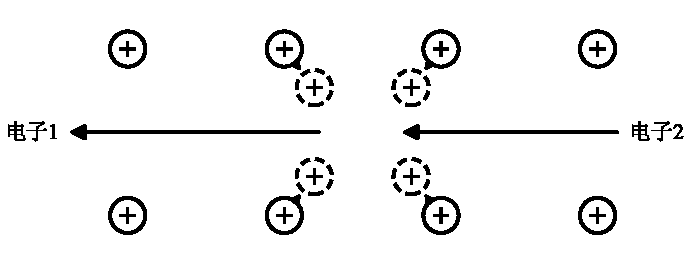
\includegraphics[width=7.5cm]{fig5-6.pdf}\\{\small 图 5.6\quad 电子-电子有效互作用}
\end{minipage}
\end{center}

我们讨论单价金属中电子与 LA 声子的互作用，根据式(5.2.22)其哈密顿量可写为
\begin{equation}
  \left.\begin{aligned}
  H_{\mathrm{ep}}&=\sum_{k,q,\sigma}\left(D_qa_qC_{k+q,\sigma}^{+}C_{k\sigma}
  +D_q^{+}a_q^{+}C_{k-q,\sigma}^{+}C_{k\sigma}\right)\\
  D_q&=-\mathrm{i}\left(\frac{N\hbar}{2M\omega_q}\right)^{1/2}V_q\left(\boldsymbol{e}_q\cdot\boldsymbol{q}\right)\\
  \boldsymbol{e}_{-q}=\boldsymbol{e}_q&\text{，}\ \omega_{-q}=\omega_q\text{，}\ \left|D_q\right|^2=\left|D_{-q}\right|^2
  \end{aligned}\right\}
\end{equation}
这里 $\sigma$ 为电子自旋，常用自旋朝上（$\uparrow$）或向下（$\downarrow$）表示，代表电子自旋在 $z$ 方向投影取 $\pm\dfrac{\hbar}{2}$ 值.为了图像清楚起见，我们先定性估计有效互作用的形式，然后再利用正则变换方法作较严格的推导.

\subsection*{1. 电子-电子有效互作用的微扰估计}

弗留里希\textsuperscript{[5]}首先利用二级玻恩散射矩阵对电子间交换 LA 声子的有效互作用进行了微扰估计，他按照下列图形所表示的两种虚声子过程（或中间过程）写出电子通过交换声子的互作用矩阵元为
\begin{equation}
\begin{aligned}
  &\sum_{m}\frac{\left\langle f\middle|H_{\mathrm{ep}}\middle|m\right\rangle
  \left\langle m\middle|H_{\mathrm{ep}}\middle|i\right\rangle}{E_i-E_m}\\
  &\quad=\sum_{q}\left|D_q\right|^2\biggl\{
  \frac{\left\langle f\middle|a_qC_{k+q,\sigma}^{+}C_{k\sigma}\middle|m_1\right\rangle
  \left\langle m_1\middle|a_q^{+}C_{k'-q,\sigma'}^{+}C_{k'\sigma'}\middle|i\right\rangle}
  {\varepsilon_{k'}-\varepsilon_{k'-q}-\hbar\omega_q}+\\
  &\qquad\frac{\left\langle f\middle|a_{-q}C_{k'-q,\sigma'}^{+}C_{k'\sigma'}\middle|m_2\right\rangle
  \left\langle m_2\middle|a_{-q}^{+}C_{k+q,\sigma}^{+}C_{k\sigma}\middle|i\right\rangle}
  {\varepsilon_k-\varepsilon_{k+q}-\hbar\omega_{-q}}\biggr\}
\end{aligned}
\end{equation}

\begin{center}
\begin{minipage}{8cm}
\centering
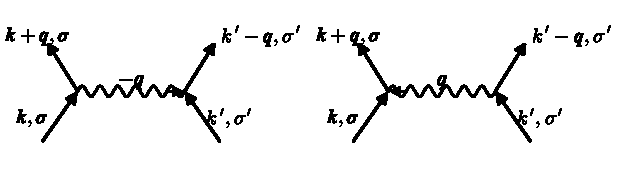
\includegraphics[width=8cm]{fig5-7.pdf}\\[0.3em]
{\small (a) $\boldsymbol{k}'$ 发射 $\boldsymbol{q}$ 声子\qquad\qquad (b) $\boldsymbol{k}$ 发射 $\left(-\boldsymbol{q}\right)$ 声子}\\[0.2em]
{\small 图 5.7\quad 电子-声子-电子互作用}
\end{minipage}
\end{center}

其中初态与终态
\begin{equation*}
\begin{aligned}
  &\left|i\right\rangle=\left|\cdots,\ n_{k\sigma},\ \cdots,\ n_{k'\sigma'},\ \cdots,\ n_{k'-q,\sigma'},\ \cdots,\ n_{k+q,\sigma},\ \cdots;\ 0\right\rangle\\
  &\left|f\right\rangle=\left|\cdots,\ \left(n_{k\sigma}-1\right),\ \cdots,\ \left(n_{k'\sigma'}-1\right),\ \cdots,\right.\\
  &\qquad\qquad\left.\left(n_{k'-q,\sigma'}+1\right),\ \cdots,\ \left(n_{k+q,\sigma}+1\right),\ \cdots;\ 0\right\rangle
\end{aligned}
\end{equation*}
为声子真空态，而两个中间态
\begin{equation*}
\begin{aligned}
  &\left|m_1\right\rangle=\left|\cdots,\ n_{k\sigma},\ \cdots,\ \left(n_{k'\sigma'}-1\right),\ \cdots,\right.\\
  &\qquad\qquad\left.\left(n_{k'-q,\sigma'}+1\right),\ \cdots,\ n_{k+q,\sigma},\ \cdots;\ 1_q\right\rangle\\
  &\left|m_2\right\rangle=\left|\cdots,\ \left(n_{k\sigma}-1\right),\ \cdots,\ n_{k'\sigma'},\ \cdots,\right.\\
  &\qquad\qquad\left.n_{k'-q,\sigma'},\ \cdots,\ \left(n_{k+q,\sigma}+1\right),\ \cdots;\ 1_{-q}\right\rangle
\end{aligned}
\end{equation*}
都有一个声子激发.$\left|m_1\right\rangle$ 与图5.7中(a)对应，$\left|m_2\right\rangle$ 与(b)对应.

利用 $\left\langle 1_q\middle|a_q^{+}\middle|0_q\right\rangle=\left\langle 0_q\middle|a_q\middle|1_q\right\rangle=1$，容易算出式(5.5.2)对声子态的平均.再考虑到散射前后能量守恒 $\varepsilon_k+\varepsilon_{k'}=\varepsilon_{k+q}+\varepsilon_{k'-q}$，可用 $\left(\varepsilon_{k+q}-\varepsilon_k\right)$ 代替第一项分母中的 $\left(\varepsilon_{k'}-\varepsilon_{k'-q}\right)$.这时两项分子的计算结果均与 $\left\langle f\middle|C_{k+q,\sigma}^{+}C_{k'-q,\sigma'}^{+}C_{k'\sigma'}C_{k\sigma}\middle|i\right\rangle$ 相等，因此，可以用一个不明显含声子算符的有效互作用矩阵元 $\left\langle f\middle|H_{\mathrm{eff}}\middle|i\right\rangle$ 代替式(5.5.2)，得
\begin{equation}
\begin{aligned}
  \left\langle f\middle|H_{\mathrm{eff}}\middle|i\right\rangle
  &=\sum_{q}\left|D_q\right|^2\biggl\{\frac{1}{\varepsilon_k-\varepsilon_{k+q}-\hbar\omega_{-q}}
  -\frac{1}{\varepsilon_k-\varepsilon_{k+q}+\hbar\omega_q}\biggr\}\times\\
  &\quad\left\langle f\middle|C_{k+q,\sigma}^{+}C_{k'-q,\sigma'}^{+}C_{k'\sigma'}C_{k\sigma}\middle|i\right\rangle
\end{aligned}
\end{equation}
由于时间反演对称 $\omega_{-q}=\omega_q$，可将上式中两项合并，最后得到与式(5.5.2)等效的互作用矩阵元
\begin{equation}
\begin{aligned}
  \left\langle f\middle|H_{\mathrm{eff}}\middle|i\right\rangle
  &=\sum_{q}\left|D_q\right|^2
  \frac{2\hbar\omega_q}{\left(\varepsilon_k-\varepsilon_{k+q}\right)^2-\left(\hbar\omega_q\right)^2}\times\\
  &\quad\left\langle f\middle|C_{k+q,\sigma}^{+}C_{k'-q,\sigma'}^{+}C_{k'\sigma'}C_{k\sigma}\middle|i\right\rangle
\end{aligned}
\end{equation}
根据式(5.5.4)，弗留里希作了大胆的猜测，他认为，电子与电子的有效互作用哈密顿量可表示为
\begin{equation}
\begin{aligned}
  H_{\mathrm{eff}}&=\frac{1}{2}\sum_{\substack{k',k,q\\ \sigma,\sigma'}}
  \frac{2\left|D_q\right|^2\hbar\omega_q}
  {\left(\varepsilon_k-\varepsilon_{k+q}\right)^2-\left(\hbar\omega_q\right)^2}
  C_{k+q,\sigma}^{+}C_{k'-q,\sigma'}^{+}C_{k'\sigma'}C_{k\sigma}\\
  &=\frac{1}{2}\sum_{\substack{k',k,q\\ \sigma,\sigma'}}
  V_{kq}C_{k+q,\sigma}^{+}C_{k'-q,\sigma'}^{+}C_{k'\sigma'}C_{k\sigma}
\end{aligned}
\end{equation}
其中 1/2 因子是为了消除 $k$，$k'$ 求和时的重复所引入的.$H_{\mathrm{eff}}$ 代表电子的非直接互作用，它与直接库仑作用不同，$H_{\mathrm{eff}}$ 可以是吸引互作用，也可以是排斥作用，具体要看系数
\begin{equation}
  V_{kq}=\frac{2\left|D_q\right|^2\hbar\omega_q}
  {\left(\varepsilon_k-\varepsilon_{k+q}\right)^2-\left(\hbar\omega_q\right)^2}
\end{equation}
是正还是负.当 $\left|\varepsilon_k-\varepsilon_{k+q}\right|<\hbar\omega_q$ 时，$V_{kq}<0$，在费密面附近 $\hbar\omega_q$ 宽度范围内电子间的 $H_{\mathrm{eff}}$ 是吸引互作用.当着这个吸引势超过屏蔽库仑（排斥）势时，金属中费密面附近的一对电子具有净吸引作用.库柏（N.Cooper）曾证明：只要费密面上一对电子间存在着吸引力，不管其大小如何，都会导致金属费密球的改组，形成电子对的束缚态，这是超导电性的基本原因，详细内容将在下一章介绍.式(5.5.5)称为弗留里希互作用，其正确性应有更为严格的推导加以证实.

\subsection*{2. 正则变换方法——中岛变换}

中岛（S.Nakajima）\textsuperscript{[6]}从电子-声子系统的总哈密顿量
\begin{equation}
\begin{aligned}
  &H=H_0+H_1\\
  &H_0=\sum_{q}\hbar\omega_qa_q^{+}a_q+\sum_{k,\sigma}\varepsilon_kC_{k\sigma}^{+}C_{k\sigma}\\
  &H_1=H_{\mathrm{ep}}=\sum_{q,k,\sigma}\left(D_qa_qC_{k+q,\sigma}^{+}C_{k\sigma}
  +D_q^{+}a_q^{+}C_{k-q,\sigma}^{+}C_{k\sigma}\right)
\end{aligned}
\end{equation}
出发，利用正则变换方法，正规地导出了弗留里希的 $H_{\mathrm{eff}}$.

对于本征值为 $E$ 的多体系统，$H\psi=E\psi$，作正则变换 $\psi=\mathrm{e}^{S}\psi'$，可求出
\begin{equation}
  H_S=\mathrm{e}^{-S}H\mathrm{e}^{S}
\end{equation}
为变换后的哈密顿量，$H_S$ 满足 $H_S\psi'=E\psi'$ 方程，它与原来的 $H$ 有相同的本征值.利用量子力学公式，可以将变换后的 $H_S$ 写为
\begin{equation}
\begin{aligned}
  H_S&=H+\left[H,S\right]+\frac{1}{2}\left[\left[H,S\right],S\right]+\cdots\\
  &=H_0+\left(H_1+\left[H_0,S\right]\right)
  +\frac{1}{2}\left[\left(H_1+\left[H_0,S\right]\right),S\right]
  +\frac{1}{2}\left[H_1,S\right]+\cdots
\end{aligned}
\end{equation}
假如认为 $H_1$ 是一阶项，可选择与 $H_1$ 同阶的变换母函数 $S$，使之满足条件：
\begin{equation}
  H_1+\left[H_0,S\right]=0
\end{equation}
这时式(5.5.9)右边第二、三项均可消去.中岛变换方法就是利用上式首先严格地消去电子-声子的一阶互作用项，然后讨论准至 $H_1$ 二阶的哈密顿量
\begin{equation}
  H_S=H_0+\frac{1}{2}\left[H_1,S\right]
\end{equation}
其中包括了电子-声子系统的全部二级过程，由此可求出电子间的二阶有效互作用 $H_{\mathrm{eff}}$.

变换的母函数 $S$ 可假设为
\begin{equation}
  S=\sum_{k,q,\sigma}\left(A_qa_qC_{k+q,\sigma}^{+}C_{k\sigma}
  +B_qa_q^{+}C_{k-q,\sigma}^{+}C_{k\sigma}\right)
\end{equation}
利用式(5.5.10)求出下列矩阵元关系式
\begin{equation*}
  \left\langle m\left|\left[H_0,S\right]\right|n\right\rangle
  =\left(E_m-E_n\right)\left\langle m\middle|S\middle|n\right\rangle
  =-\left\langle m\middle|H_1\middle|n\right\rangle
\end{equation*}
其中 $\left|n\right\rangle$ 及 $\left|m\right\rangle$ 为 $H_0$ 的本征态.由此得到变换母函数 $S$ 的矩阵元
\begin{equation}
  \left\langle m\middle|S\middle|n\right\rangle
  =\frac{\left\langle m\middle|H_1\middle|n\right\rangle}{E_n-E_m}
\end{equation}
将 $H_1$ 代入上式立刻求得系数 $A_q$ 和 $B_q$ 为
\begin{equation}
  \left.\begin{aligned}
  A_q&=D_q\left(\varepsilon_k+\hbar\omega_q-\varepsilon_{k+q}\right)^{-1}\\
  B_q&=D_q^{+}\left(\varepsilon_k-\varepsilon_{k-q}-\hbar\omega_q\right)^{-1}
  \end{aligned}\right\}
\end{equation}
因此
\begin{equation}
  S=\sum_{k,q,\sigma}\biggl(D_q\frac{a_qC_{k+q,\sigma}^{+}C_{k\sigma}}
  {\varepsilon_k-\varepsilon_{k+q}+\hbar\omega_q}
  +D_q^{+}\frac{a_q^{+}C_{k-q,\sigma}^{+}C_{k\sigma}}
  {\varepsilon_k-\varepsilon_{k-q}-\hbar\omega_q}\biggr)
\end{equation}
如果直接用式(5.5.15)计算 $\frac{1}{2}\left[H_1,S\right]$，可求得不含声子算符项以及含有类型为 $a^{+}a$、$aa$ 及 $a^{+}a^{+}$ 声子算符的项.在不含声子算符项中又包括 $C^{+}C$ 类型的电子自能修正和 $C_1^{+}\,C_2^{+}\,C_3C_4$ 型的电子间的有效互作用 $H_{\mathrm{eff}}$.除 $H_{\mathrm{eff}}$ 外的其它项代表电子-声子互作用对电子和声子的自能修正以及双声子过程等，这些都不是我们感兴趣的，必须去掉.选出 $H_{\mathrm{eff}}$ 的一种简单的办法是，对于 $\frac{1}{2}\left[H_1,S\right]$ 求声子真空态的对角平均.这样做能够很自然地去掉二阶互作用中含声子算符的诸项，求得只含电子算符的部分，暂记为 $H_{\mathrm{el}}$
\begin{equation}
\begin{aligned}
  H_{\mathrm{el}}&=\left\langle 0\left|\frac{1}{2}\left[H_1,S\right]\right|0\right\rangle\\
  &=\frac{1}{2}\sum_{q}\left\{\left\langle 0\ \middle|H_1\middle|\ 1_q\right\rangle
  \left\langle 1_q\ \middle|S\middle|\ 0\right\rangle-\right.\\
  &\quad\left.\left\langle 0\ \middle|S\middle|\ 1_q\right\rangle
  \left\langle 1_q\ \middle|H_1\middle|\ 0\right\rangle\right\}
\end{aligned}
\end{equation}
若再人为地略去电子自能修正，即可找出电子间的有效互作用 $H_{\mathrm{eff}}$.这时很容易算出上式中对声子态的矩阵元为
\begin{equation}
  \left.\begin{aligned}
  \left\langle 0\middle|H_1\middle|1_q\right\rangle&=\sum_{k,\sigma}D_qC_{k+q,\sigma}^{+}C_{k\sigma}\\
  \left\langle 1_q\middle|H_1\middle|0\right\rangle&=\sum_{k,\sigma}D_q^{+}C_{k-q,\sigma}^{+}C_{k\sigma}\\
  \left\langle 1_q\middle|S\middle|0\right\rangle&=\sum_{k,\sigma}D_q^{+}C_{k-q,\sigma}^{+}C_{k\sigma}
  \left(\varepsilon_k-\varepsilon_{k-q}-\hbar\omega_q\right)^{-1}\\
  \left\langle 0\middle|S\middle|1_q\right\rangle&=\sum_{k,\sigma}D_qC_{k+q,\sigma}^{+}C_{k\sigma}
  \left(\varepsilon_k-\varepsilon_{k+q}+\hbar\omega_q\right)^{-1}
  \end{aligned}\right\}
\end{equation}
将它们代入式(5.5.16)
\begin{equation}
  H_{\mathrm{el}}=\frac{1}{2}\sum_{\substack{k,k',q\\ \sigma,\sigma'}}\left|D_q\right|^2
  \left\{\frac{C_{k+q,\sigma}^{+}C_{k\sigma}C_{k'-q,\sigma'}^{+}C_{k'\sigma'}}
  {\varepsilon_{k'}-\varepsilon_{k'-q}-\hbar\omega_q}
  -\frac{C_{k+q,\sigma}^{+}C_{k\sigma}C_{k'-q,\sigma'}^{+}C_{k'\sigma'}}
  {\varepsilon_k-\varepsilon_{k+q}+\hbar\omega_q}\right\}
\end{equation}
利用 $\boldsymbol{q}\to-\boldsymbol{q}$ 时的对称性 $\omega_{-q}=\omega_q$，$\left|D_{-q}\right|^2=\left|D_q\right|^2$，并对调 $\left(\boldsymbol{k},\sigma\right)$ 与 $\left(\boldsymbol{k}',\sigma'\right)$，可将等式花括号中第一项的分母变换为 $\left(\varepsilon_k-\varepsilon_{k+q}-\hbar\omega_q\right)$，而分子变为 $C_{k'-q,\sigma'}^{+}C_{k'\sigma'}C_{k+q,\sigma}^{+}C_{k\sigma}$，再利用对易关系作整理，并略去自能修正项，最后求得电子-声子-电子的有效互作用为
\begin{equation}
  H_{\mathrm{eff}}=\frac{1}{2}\sum_{\substack{k,k',q\\ \sigma,\sigma'}}V_{kq}
  C_{k+q,\sigma}^{+}C_{k'-q,\sigma'}^{+}C_{k'\sigma'}C_{k\sigma}
\end{equation}
其中
\begin{equation}
  V_{kq}=\frac{2\left|D_q\right|^2\hbar\omega_q}
  {\left(\varepsilon_k-\varepsilon_{k+q}\right)^2-\left(\hbar\omega_q\right)^2}
\end{equation}
证实了弗留里希的微扰估计式(5.5.5).以上中岛变换方法是凝聚态理论中寻找有效相互作用的一种传统方法，适用于电子与玻色子相互作用的一切系统，在氧化物高温超导体中也常被采用.

在结束本节时，我们还应当对 $\left|\varepsilon_k-\varepsilon_{k+q}\right|<\hbar\omega_q$ 时 $V_{kq}<0$ 作出定性解释.由于晶格畸变以 $\omega_q$ 频率响应电子(1)（参考图5.6），而电子(1)在吸收声子后从 $\varepsilon_k$ 过渡到 $\varepsilon_{k+q}$ 态的快慢由 $\omega$ 量度 $\left(\hbar\omega\equiv\left|\varepsilon_k-\varepsilon_{k+q}\right|\right)$，这里 $\omega$ 代表跃迁频率.显然，只有在 $\omega<\omega_q$ 时，离子实才来得及跟随电子产生晶格畸变并导致电子(1)周围有正电荷集中，从而使得进入畸变区的另一个电子(2)也受到吸引，这样就在电子(1)与(2)之间形成间接的吸引互作用，通常称为声子吸引机制.反之，当 $\omega>\omega_q$ 时，离子实来不及响应电子，这时(1)与(2)电子之间仍为库仑排斥作用.这就是在费密面附近能壳区 $\left|\varepsilon_k-\varepsilon_{k+q}\right|<\hbar\omega_q$ 内 $V_{kq}<0$（吸引），而在其外 $\left|\varepsilon_k-\varepsilon_{k+q}\right|>\hbar\omega_q$ 为 $V_{kq}>0$（排斥）的物理原因.

\begin{canKao}
\begin{enumerate}[label={[\arabic*]}, leftmargin=2.2em, itemsep=0pt]
\item Bardeen J, Shockley W. Phys Rev, 1950, 80: 72
\item Nordheim L. Ann Phys, 1931, 9: 607
\item Bohm D, Staver I. Phys Rev, 1951, 84: 836
\item Fr\"{o}hlich H et al. Phil. Mag, 1950, 41: 221
\item Fr\"{o}hlich H. Phys Rev, 1950, 79: 845
\item Nakajima S. Adv Phys, 1953, 4: 363
\end{enumerate}
\end{canKao}

% ============================================================
%  第六章 超导电性的微观理论（§1–§10 + 章末参考文献）
%  底本：高等教育出版社《固体理论》第二版；原书印刷页 159–228
%  （PDF 页 = 印刷页 + 20）
%  公式编号自检：§2 (6.2.1)–(6.2.12)；§3 (6.3.1)–(6.3.13)；
%    §4 (6.4.1)–(6.4.47)；§5 (6.5.1)–(6.5.59)（(6.5.27a/b)、
%    (6.5.57a/b) 为原书自带二级编号，用 subequations 环境照录，
%    与 ch04 体例一致）；§6 (6.6.1)–(6.6.28)；§7 (6.7.1)–(6.7.20)；
%    §8 (6.8.1)–(6.8.52)；§9 (6.9.1)–(6.9.19)；
%    §10 (6.10.1)–(6.10.68)（(6.10.12a/b) 同上照录）。
%    全章自动编号 315 个，无缺号。
%
%  任务单所列 22 处"缺号"逐条对照原书页面判定（均非原书跳号）：
%    (6.3.7)  原书 p165 在号（OCR tag 多一句点未识别）；
%    (6.4.11) 原书 p168 在号（OCR 误把本式标为 (6.4.10)、又丢
%             (6.4.10) 之号，已按 p188 归位）；
%    (6.4.30)(6.4.31)(6.4.35)(6.4.39) OCR tag 残缺，公式原书均在
%             （p171–173）；
%    (6.5.16)(6.5.34) OCR tag 残缺，公式原书在（p180、183）；
%    (6.5.27) 原书即分 a/b（p182）；(6.5.57) 原书即分 a/b（p187）；
%    (6.5.52) 原书 p186 在号，OCR 丢式留号，已按页面补排；
%    (6.6.26) 原书 p191 在号，OCR 丢号留式；
%    (6.8.4)(6.8.8)(6.8.13)(6.8.15)(6.8.30)(6.8.48) OCR tag 残缺，
%             公式原书均在（p197–206）；
%    (6.8.18) 原书 p199 为第 5 个矩阵元（₀<0|ĵ₁|0>₀=0），OCR 丢式
%             留号，已按页面补排；
%    (6.10.8) OCR tag 残缺（p212）；(6.10.12) 原书即分 a/b（p213）；
%    (6.10.66) OCR tag 残缺（p226）。
%
%  已修正的 OCR/原书错误（除全角句点转"."、删 ~ 间隔符、收紧
%  \mathrm{d}、拆开行内公式与中文等常规项外）：
%  1. 章名 OCR"超导性的微观理论"→"超导电性的微观理论"（原书
%     p179 章题及各页页眉）。
%  2. §1 化学式按原书复原：La$_2$-aSr$_x$→La$_{2-x}$Sr$_x$、
%     O→O（数字 0 误识）、Π$_2$Ba$_2$…→Tl$_2$Ba$_2$…（p179）。
%  3. (6.2.1)(6.2.3)(6.2.4) OCR 求和上下标错乱，按 p181–182 复原
%     为 1/2 Σ_{q,k1,k2;σ1,σ2}；(6.2.4) 末因子重复的 C_{k1,σ1} 删一。
%  4. Ĥ 无编号三行式首行 C⁺_{-k',σ}→C⁺_{-k',-σ}（与 (6.2.8) 及
%     其↑/↓展开一致，p183）。
%  5. (6.2.11) 下文 OCR"约化哈密顿量选用H的理由是……总粒子 H̄ 数
%     不守恒"语序错乱，按 p164 复原。
%  6. (6.3.10) OCR 求和项漏撇号 a^*(k)a(k)，按 p165 复原为
%     a^*(k)a(k')。
%  7. §4 章首 OCR 残句"设 v_k 是……u代表……则BCS u_k 超导基态"
%     按 p167 复原。
%  8. (6.4.9)(6.4.15)(6.4.2)(6.4.3)(6.5.5)(6.9.x)(6.10.5) 等右括号
%     按原书补全；(6.4.19)(6.4.21)"ξ_k=|ε_k|"OCR 乱码按 p169 复原。
%  9. (6.4.21) 后两个未编号 cases 中 OCR 乱码按 p169 复原为
%     "费密球外(内)产生(消灭)电子(空穴)"。
% 10. (6.4.25) 末尾 OCR 杂符"( 0 )"已删（p171）。
% 11. (6.4.29) 末"[g(0)V<<1]"OCR 乱码按 p171 复原。
% 12. (6.4.35) 前文"将变换公式(6.4.14)代入式(6.4.33)"原书引号有误：
%     所代换的是 α=C 变换式(6.4.9)，(6.4.14) 为 u²+v²=1 无法代入，
%     按 p172 更正为"(6.4.9)"。
% 13. §4.5 OCR 重复句段（"质心速度为 等于ħ(2δk)……此库柏对运动的
%     电流密度为"两见）按 p195 去重。
% 14. §5 章首 (6.5.2) OCR"\doteq"→"="（p177 印刷为等号）。
% 15. 表 6.1 OCR 串行（Cd–Pb 各列错位），按 p182 原表逐格复原。
% 16. (6.5.19) 脚注①"详见附录E."OCR 漏失，按 p181 页脚补录；
%     (6.10.12a) 前 ψ_0 之脚注①"确切地说，ψ_0只是大块超导样品
%     远离界面处的序参数值."OCR 漏失，按 p213 页脚补录。
% 17. (6.5.48) OCR cases 乱码按 p205 复原（N相/S相两条）。
% 18. (6.5.57) 前一公式块上方混入的图例残字"BCS 理论曲线 实验曲线"
%     已删（属图 6.12 内文字，p187）。
% 19. §6 (6.6.4) 末逗号及 (6.6.12) 末撇号杂符已删；(6.6.13) 求和号
%     下标按 (6.6.10) 统一为 k'，θ(ε+εV)→θ(ε+eV)（p189）。
% 20. §6 (6.6.15)(6.6.21)(6.6.26) 三块严重乱码按 p190–191 重排；
%     (6.6.21) OCR 尾部衍出的孤立"A"已删。
% 21. (6.7.10)(6.7.11) 中"ξ_0Δc"按 p194–195 复原为"ξ_0Λc"
%     （Λ 为 (6.7.1) 定义的伦敦参量）；指数因子 e^{-ħ√ξ_0} 等乱码
%     复原为 e^{-R/ξ_0}。
% 22. 原书 p194 印刷错误："通过∇×B=(4π/e)j_s"→(4π/c)j_s
%     （麦克斯韦方程，与 p193 式用 c 一致）。
% 23. (6.8.6) OCR 丢积分号、和号上标杂符"e\hat{h}"已按 p197 清理。
% 24. (6.8.9) 下文 j_2 平均式中 C⁺_{-k}C⁺_{-k-q}→C⁺_{-k}C_{-k-q}
%     （基态占据数平均，p198）。
% 25. (6.8.14)(6.8.15) OCR 乱码按 p199 复原；分母 E_0−E_l 的 l 为
%     中间态标号（OCR 误作 1）。
% 26. (6.8.17)(6.8.18) 拆分归位：前两矩阵元为 (6.8.17)，后三式为
%     (6.8.18)（p199）。
% 27. (6.8.19)(6.8.20)(6.8.24)(6.8.30)(6.8.33)(6.8.35)(6.8.39)
%     (6.8.48) 等块 OCR 乱码/残缺按 p199–206 重排复原；
%     (6.8.35) 中√(ε_2+ζ²)→√(ε²+Δ²)、arsinh 复原。
% 28. §8 章首末尾衍字"2"已删（p196–197）。
% 29. (6.8.42)(6.8.45)(6.8.46) OCR 上下标错乱按 p205 复原
%     （(6.8.45) 末项为 α⁺_{-k}α_{-k}）。
% 30. §9 (6.9.1) 末尾杂符"]"已删；(6.9.17) OCR"<0.1 N̂|0>"→
%     "<0|N̂|0>"（p209）。
% 31. §10 (6.10.3) OCR 分数乱码按 p211 复原；(6.10.8) tag"(.8)"
%     归还本式；(6.10.10) 分子按 p212 复原。
% 32. (6.10.30)"n=整数"OCR 乱码按 p217 复原；(6.10.34) 原书
%     "[7ζ(3)_n]^{1/2}"为"[7ζ(3)n]^{1/2}"（n 为电子密度，与下文
%     m*=2m 对应关系一致），照此排。
% 33. §10.3 特征参量"$\star(T)$"→κ(T)（p213）。
% 34. §10.5 SQUID 一段 OCR 的 \tilde{Φ} 按原书 p245–246 全部改为 Φ。
% 35. 原书 p223 印刷错误："ω_0=483.6×10 Hz"→483.6×10⁷ Hz
%     （V_0=10 μV 时 2eV_0/h≈4.84×10⁹ Hz=483.6×10⁷ Hz）。
% 36. 图 6.12 图注原书"[1−(T/T_0)²]"→[1−(T/T_c)²]（与式(6.5.58)
%     一致，p207）。
% 37. 文献[7][16]中文条目"．"转"."；其余西文条目照原书
%     （[3]"Mahen G.D."、[6]"Giaever L."原书如此，未改）。
%  遗留问题：
%  · 图 6.1–6.23 均为占位图（figures/fig6-N.pdf）；图 6.15 原书在
%    p216 右侧（印刷 196），manifest 无独立裁剪，重绘代理负责绘制，
%    图注按原书补"皮帕的 K(q)"；图 6.18 manifest 无裁剪图（原书
%    p238，印刷 218），图注仅"图 6.18"；图 6.16 原书图注仅"图 6.16"。
% ============================================================
\chapter{超导电性的微观理论}

\section{基本性质}

人们将低温下直流电阻消失的现象称为超导电性，具有超导电性的材料叫做超导体.目前已发现有一半的金属元素和成百上千种合金与化合物是超导体，但是它们的超导转变温度 $T_{\mathrm{c}}$ 较低，直至20世纪80年代中期，$T_{\mathrm{c}}$ 未能突破30K大关，称之为常规超导体.1986年以后，人们在多元的铜氧化合物中发现了一系列 $T_{\mathrm{c}}$ 超过30K的超导体，如 $\mathrm{La}_{2-x}\mathrm{Sr}_{x}\mathrm{CuO}_{4}$（$x=0.15$，$T_{\mathrm{c}}=39$ K）、$\mathrm{YBa}_{2}\mathrm{Cu}_{3}\mathrm{O}_{7}$（92K）、$\mathrm{Bi}_{2}\mathrm{Sr}_{2}\mathrm{Ca}_{2}\mathrm{Cu}_{3}\mathrm{O}_{10}$（110K）、$\mathrm{Tl}_{2}\mathrm{Ba}_{2}\mathrm{Ca}_{2}\mathrm{Cu}_{3}\mathrm{O}_{10}$（125K），以及目前公认的最高 $T_{\mathrm{c}}$ 材料 $\mathrm{HgBa}_{2}\mathrm{Ca}_{2}\mathrm{Cu}_{3}\mathrm{O}_{8+\delta}$（133K，加压力 $T_{\mathrm{c}}$ 可达160K以上）等等，其中绝大多数可在液氮条件下应用，被称为高温超导体，我们将在下一章中作专门的介绍.本章仅限于介绍常规超导体的基本物理性能.

超导体的基本属性可由下列3个特征表示：

\subsection*{1. 超导态是一种新的凝聚态}

例如冷却金属Sn时发现，$T=T_{\mathrm{c}}=3.7$ K处比热容有跃变，在 $T_{\mathrm{c}}$ 温度以下金属Sn的电子比热容不再与T成线性关系，而是当 $T\ll T_{\mathrm{c}}$ 时变为指数式的温度关系（图6.1），表现出反常，说明 $T<T_{\mathrm{c}}$ 时Sn处于一种新的热力学状态.究竟发生了什么变化呢？X射线的实验结果表明晶格结构并无变化，也不是铁磁或反铁磁转变，因为Sn没有磁性.令人惊异的新性质是在 $T<T_{\mathrm{c}}$ 时直流电阻变为零，若将Sn制成金属环，则环中感应的电流可长期持续不衰.这种持续电流称为超电流，而可以产生超电流的这种新的热力学状态也就称为超导态.

实验还证明，$T<T_{\mathrm{c}}$ 时超导态的自由能比正常态低.因为，必须加磁场 $H_{\mathrm{c}}$ 才能破坏超导性，使金属恢复电阻，回到正常态.$H_{\mathrm{c}}$ 称为超导体的临界磁场，其经验规律为，$H_{\mathrm{c}}(T)=H_{\mathrm{c}}(0)\left[1-(T/T_{\mathrm{c}})^{2}\right]$，如图6.2所示.在 $T=0$ K时超导态与正常态的自由能之差称为超导凝聚能.根据热力学，凝聚能等于 $H_{\mathrm{c}}^{2}(0)/8\pi$，约为 $10^{-8}$ eV量级.从比热容测量的 $\Delta$ 值可以证实凝聚能正比于 $g(0)\Delta^{2}$，$g(0)$ 是费密面上一种自旋取向电子的态密度.

比热容曲线中，指数因子 $\exp(-\Delta/k_{\mathrm{B}}T)$ 的出现还说明超导态中单粒子激发至少要 $\Delta$ 能量，也就是超导态中不存在 $\delta E=0$ 的准粒子激发，因此超导体的第二个重要特征是存在能隙.

\begin{center}
\begin{minipage}{6.5cm}
\centering
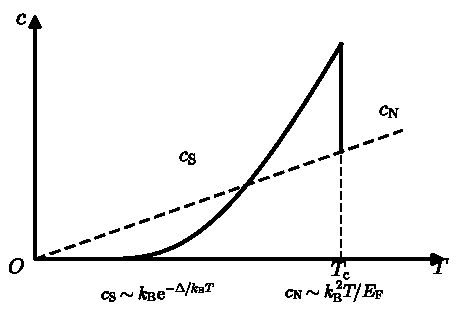
\includegraphics[width=6.5cm]{fig6-1.pdf}\\{\small 图 6.1\quad 超导体的电子比热容}
\end{minipage}
\end{center}

\begin{center}
\begin{minipage}{6cm}
\centering
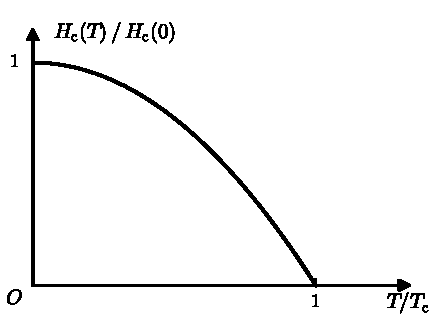
\includegraphics[width=6cm]{fig6-2.pdf}\\{\small 图 6.2\quad 超导体的临界磁场}
\end{minipage}
\end{center}

\subsection*{2. 存在能隙}

现在已有大量事实证明超导体中准粒子激发存在能隙，其中最有力的证据是隧道效应.若用很薄的氧化层（约2.5nm）将超导体（S）与正常金属（N）隔开，就在S与N之间形成了势垒.根据量子力学隧道效应理论，单电子可以穿透势垒，其隧穿电流I应与外加电压V成正比.但是，实验发现当 $T<T_{\mathrm{c}}$ 时，V必须大于 $(\Delta/e)$ 才有隧道电流，只有当 $T>T_{\mathrm{c}}$ 时才是直线，它们分别对应于图6.3中的实线与虚线.这一事实直接地证明了，从超导相中激发出一个准粒子至少要 $\Delta$ 能量，即存在能隙.超导体中的超声衰减与 $\exp(-\Delta/k_{\mathrm{B}}T)$ 成正比，同样表明有能隙.这些实验说明在费密面附近电子能谱发生了显著变化，不再是金属的费密球分布（因为在费密球面上有 $\delta E=0$ 的单粒子激发），费密球将改组.20世纪50年代初期人们做同位素实验又进一步发现，超导转变温度与晶格离子的同位素质量有 $T_{\mathrm{c}}M^{\alpha}=$ 常数的关系，其中 $\alpha$ 约等于1/2.这一发现说明超导转变与电子声子相互作用有关，其后的理论工作，都集中于从电子-声子相互作用证明能隙存在.

\begin{center}
\begin{minipage}{5cm}
\centering
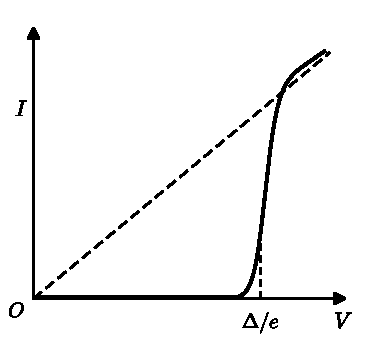
\includegraphics[width=5cm]{fig6-3.pdf}\\{\small 图 6.3\quad 隧道效应}
\end{minipage}
\end{center}

\subsection*{3. 迈斯纳效应}

迈斯纳效应指的是，在超导态弱磁场不能透入宏观样品内部，超导体对于弱场是完全逆磁体，这也是早期发现的超导特性.以后又发现对于超导合金，磁场可以透入超导体内部，但不破坏超导性，持续电流仍然存在，这类超导体称为第二类超导体，有迈斯纳效应的超导体则称为第一类超导体.对于第一类超导体，磁场超过 $H_{\mathrm{c}}(T)$ 以后，磁力线将透入样品内部，同时超导态也就被破坏，恢复为正常态.本章限于篇幅将着重于讨论第一类超导体.

对于大块纯金属样品只要证明了超导相的凝聚特性（凝聚能和能隙）就可以解释常规超导体的诸实验事实.巴丁（Bardeen）、库柏（Cooper）和施里弗（Schrieffer）（以后简称BCS）认为电子间通过交换虚声子所产生超导基态是，费密面附近相反动量及自旋的电子对通过吸引互作用形成了束缚电子对状态，称为库柏对组态.这一组态比正常费密球分布的能量要低 $g(0)\Delta^{2}$ 量级，这就是超导相的凝聚能.问题的新颖之处还在于，从这个基态的任何单粒子激发都要拆开库柏对，付出 $E_{k}=\sqrt{\varepsilon_{k}^{2}+\Delta^{2}}$ 的能量，其中 $\varepsilon_{k}$ 代表从费密能 $E_{\mathrm{F}}$ 算起的自由电子能量.因此，在费密面上激发一个准粒子至少要 $\Delta$ 能量，从而证明了能隙存在.由此出发可以解释常规超导体中的超导持续电流，迈斯纳效应和比热容的反常变化等一系列超导现象.我们将在本章中系统地介绍BCS超导理论及其对常规超导体的应用.习惯上，人们又将常规超导体称为BCS超导体.

\section{BCS约化哈密顿量}

现在分析电子交换虚声子的有效互作用
\begin{equation}
  H_{\mathrm{eff}}=\frac{1}{2}\sum_{\substack{q,\,k_{1},\,k_{2}\\\sigma_{1},\,\sigma_{2}}}
  V_{k_{1},q}\,C^{+}_{k_{1}+q,\,\sigma_{1}}C^{+}_{k_{2}-q,\,\sigma_{2}}
  C_{k_{2},\,\sigma_{2}}C_{k_{1},\,\sigma_{1}}
\end{equation}
根据式(5.5.21)其中互作用系数为
\begin{equation}
  V_{k_{1},q}=|D_{q}|^{2}
  \frac{2\hbar\omega_{q}}{(E_{k_{1}+q}-E_{k_{1}})^{2}-(\hbar\omega_{q})^{2}}
\end{equation}
在费密面附近 $|E_{k_{1}+q}-E_{k_{1}}|<\hbar\omega_{q}\approx\hbar\omega_{\mathrm{D}}$ 能壳内 $V_{k_{1},q}<0$，$H_{\mathrm{eff}}$ 为吸引互作用，在能壳外 $V_{k_{1},q}>0$，为排斥互作用，这里 $\omega_{\mathrm{D}}$ 为声子的德拜频率，$\hbar\omega_{\mathrm{D}}\sim10^{-2}$ eV.由于声学模声子的最大态密度在 $\omega_{\mathrm{D}}$ 附近，人们可以将式(6.2.2)中厚度随 $\omega_{q}$ 变化的吸引区近似用费密面附近厚度为 $2\hbar\omega_{\mathrm{D}}$ 的固定能壳区代替，这是一种合理的简化.此外，金属中电子还存在直接库仑作用，可以用屏蔽库仑势表示
\begin{equation}
  H_{\mathrm{coul}}=\frac{1}{2}\sum_{\substack{q,\,k_{1},\,k_{2}\\\sigma_{1},\,\sigma_{2}}}
  \frac{4\pi e^{2}}{q^{2}+\lambda^{2}}C^{+}_{k_{1}+q,\,\sigma_{1}}C^{+}_{k_{2}-q,\,\sigma_{2}}
  C_{k_{2},\,\sigma_{2}}C_{k_{1},\,\sigma_{1}}
\end{equation}
$H_{\mathrm{coul}}$ 是电子间的排斥势.如果电子与声子的耦合常数适当大，则在费密面附近 $2\hbar\omega_{\mathrm{D}}$ 能壳内吸引势 $V_{k_{1},q}$ 可以超过屏蔽库仑势 $\dfrac{4\pi e^{2}}{q^{2}+\lambda^{2}}$，从而产生电子之间的净吸引互作用，这是产生超导凝聚的原因.

巴丁等人认为在 $2\hbar\omega_{\mathrm{D}}$ 能壳外的排斥相互作用可以略去，而能壳内的净吸引互作用 $(V_{k_{1},q}+\frac{4\pi e^{2}}{q^{2}+\lambda^{2}})$ 可近似用常数代替，这时电子之间的相互作用写成下列简化形式
\begin{equation}
  H'=-\frac{1}{2}V\sum_{\substack{q,\,k_{1},\,k_{2}\\\sigma_{1},\,\sigma_{2}}}
  C^{+}_{k_{1}+q,\,\sigma_{1}}C^{+}_{k_{2}-q,\,\sigma_{2}}
  C_{k_{2},\,\sigma_{2}}C_{k_{1},\,\sigma_{1}}
\end{equation}
其中V为正量，而且仅在 $|E_{k_{1}+q}-E_{k_{1}}|<\hbar\omega_{\mathrm{D}}$ 区内 $V\neq0$.物理上，BCS的这一简化就是，在讨论电子间的净吸引互作用时，假定它与取向无关，相当于取各向同性的s波散射近似.在§4中我们将看到，正是此假定导致超导配对的能隙与电子间的相对取向无关，使声子机制的BCS超导体成为各向同性配对的超导体.

根据式(6.2.4)，一对电子 $(\boldsymbol{k}_{1},\sigma_{1})$ 和 $(\boldsymbol{k}_{2},\sigma_{2})$ 散射后变为 $(\boldsymbol{k}_{1}+\boldsymbol{q},\sigma_{1})$ 和 $(\boldsymbol{k}_{2}-\boldsymbol{q},\sigma_{2})$，总波矢守恒，令
\begin{equation*}
  \boldsymbol{K}=\boldsymbol{k}_{1}+\boldsymbol{k}_{2}
\end{equation*}
将 $\boldsymbol{H}'$ 改写为
\begin{equation*}
  H'=-\frac{V}{2}\sum_{\substack{q,\,k_{1},\,k_{2}\\\sigma_{1},\,\sigma_{2}}}
  C^{+}_{k_{1}+q,\,\sigma_{1}}C^{+}_{K-k_{1}-q,\,\sigma_{2}}
  C_{K-k_{1},\,\sigma_{2}}C_{k_{1},\,\sigma_{1}}
\end{equation*}
再设 $\boldsymbol{k}'=\boldsymbol{k}+\boldsymbol{q}$，$\boldsymbol{k}=\boldsymbol{k}_{1}$，$\sigma_{1}=\sigma$，$\sigma_{2}=\sigma'$，则 $\boldsymbol{H}'$ 可按总波矢K分类
\begin{equation}
  H'=\sum_{K}H'_{K}
\end{equation}
其中
\begin{equation}
  H'_{K}\equiv-\frac{V}{2}\sum_{k,\,k',\,\sigma,\,\sigma'}
  C^{+}_{k',\,\sigma}C^{+}_{K-k',\,\sigma'}C_{K-k,\,\sigma'}C_{k,\,\sigma}
\end{equation}
代表系统中总波矢为K的电子对间相互作用.对于不同的K，具有吸引互作用的电子对数目不同，由图6.4中阴影区绕K轴转成的体积决定.显然，$\boldsymbol{K}\neq0$ 时，这个体积随K值变化不大.但是，$\boldsymbol{K}=0$ 情况十分特殊，这时电子对吸引区就是能量差为 $2\hbar\omega_{\mathrm{D}}$ 的两同心球间体积，它大于任一个"$\boldsymbol{K}\neq0$ 对"的相体积.因此 $\boldsymbol{K}=0$ 电子对占有最大相体积.换句话说，$H'_{K=0}$ 的散射互作用比 $H'_{K\neq0}$ 占更大优势，可以略去式(6.2.5)中 $\boldsymbol{K}\neq0$ 项，只取K=0电子对项
\begin{equation}
  H'=-\frac{V}{2}\sum_{k,\,k',\,\sigma,\,\sigma'}
  C^{+}_{k',\,\sigma}C^{+}_{-k',\,\sigma'}C_{-k,\,\sigma'}C_{k,\,\sigma}
\end{equation}
式(6.2.7)代表准动量相反的电子对的吸引互作用，其中 $\sigma'$ 可取 $\pm\sigma$ 两种状态，正号对应于两电子自旋平行，负号为反平行取向.由于泡利不相容原理将限制自旋平行电子在位置空间靠拢，因此式(6.2.7)中 $\sigma'=\sigma$ 项的贡献比 $\sigma'=-\sigma$ 项小，也可略去，最后将互作用取为
\begin{equation}
  H'=-\frac{V}{2}\sum_{k,\,k',\,\sigma}
  C^{+}_{k',\,\sigma}C^{+}_{-k',\,-\sigma}C_{-k,\,-\sigma}C_{k,\,\sigma}
\end{equation}

\begin{center}
\begin{minipage}{6cm}
\centering
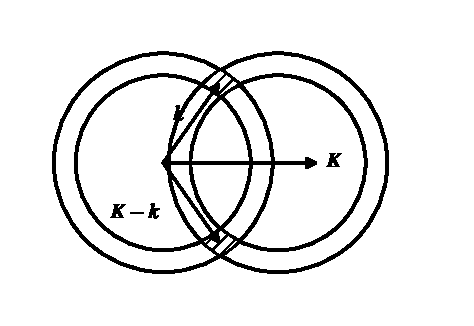
\includegraphics[width=6cm]{fig6-4.pdf}\\{\small 图 6.4\quad 总波矢为K时电子对的吸引区（阴影区）}
\end{minipage}
\end{center}

加上电子能量即为总哈密顿量
\begin{equation*}
\begin{aligned}
  \hat{H}&=\sum_{k,\,\sigma}E_{k}C^{+}_{k,\,\sigma}C_{k,\,\sigma}
  -\frac{V}{2}\sum_{k,\,k',\,\sigma}
  C^{+}_{k',\,\sigma}C^{+}_{-k',\,-\sigma}C_{-k,\,-\sigma}C_{k,\,\sigma}\\
  &=\sum_{k}E_{k}\left(C^{+}_{k\uparrow}C_{k\uparrow}
  +C^{+}_{k\downarrow}C_{k\downarrow}\right)\\
  &\quad-\frac{V}{2}\sum_{k,\,k'}\left(C^{+}_{k'\uparrow}C^{+}_{-k'\downarrow}
  C_{-k\downarrow}C_{k\uparrow}
  +C^{+}_{k'\downarrow}C^{+}_{-k'\uparrow}C_{-k\uparrow}C_{k\downarrow}\right)
\end{aligned}
\end{equation*}
对上式右边最后一项作代换 $(k,k')\to(-k,-k')$ 并考虑到 $E_{-k}=E_{k}$，整理后得
\begin{equation}
  \hat{H}=\sum_{k}E_{k}\left(C^{+}_{k\uparrow}C_{k\uparrow}
  +C^{+}_{-k\downarrow}C_{-k\downarrow}\right)
  -V\sum_{k,\,k'}C^{+}_{k'\uparrow}C^{+}_{-k'\downarrow}C_{-k\downarrow}C_{k\uparrow}
\end{equation}
这就是BCS理论用于描述超导基态的哈密顿量，其基本假定是，在费密面附近准动量和自旋都相反的电子之间的吸引互作用是产生超导凝聚的主要原因.由于式(6.2.9)中 $(k,\uparrow)$ 或 $(-k,\downarrow)$ 总是同时出现，可采用简化记号，令k代表 $(k,\uparrow)$，$-k$ 代表 $(-k,\downarrow)$，则BCS的哈密顿量简化为
\begin{equation}
  \hat{H}=\sum_{k}E_{k}\left(C^{+}_{k}C_{k}+C^{+}_{-k}C_{-k}\right)
  -V\sum_{k,\,k'}C^{+}_{k'}C^{+}_{-k'}C_{-k}C_{k}
\end{equation}
在以后的讨论中，将从下列约化哈密顿量出发：
\begin{equation}
  \overline{H}=\hat{H}-E_{\mathrm{F}}\hat{N}
  =\sum_{k}\varepsilon_{k}\left(C^{+}_{k}C_{k}+C^{+}_{-k}C_{-k}\right)
  -V\sum_{k,\,k'}C^{+}_{k'}C^{+}_{-k'}C_{-k}C_{k}
\end{equation}
其中
\begin{equation}
  \varepsilon_{k}=E_{k}-E_{\mathrm{F}}
\end{equation}
代表从费密面算起的自由电子能量，吸引互作用V仅在 $|\varepsilon_{k}|<\hbar\omega_{\mathrm{D}}$ 区域内不等于零.约化哈密顿量选用 $\overline{H}$ 的理由是因为在超导问题中总粒子数不守恒（详见§9），所以取 $\overline{H}=\hat{H}-E_{\mathrm{F}}\hat{N}$，相当于用热力学势代替自由能讨论粒子数可变系统.

\section{库柏对}

为了研究费密面附近吸引互作用对系统的电子状态和能量将产生什么影响，库柏\textsuperscript{[1]}讨论了 $T=0$ K时在已被填满的费密球外附加两个电子的相互作用问题.为使问题简化，库柏假设费密球内电子可当自由电子处理.因此，费密球的存在仅起着禁止附加电子占据 $k<k_{\mathrm{F}}$ 状态的作用，可以完全忽略费密球内电子被散射到球外的复杂情况，只考虑附加电子之间的相互作用.这样，只需处理二体散射问题.

设这两个附加电子具有相反的动量和自旋，其状态由 $C^{+}_{k}C^{+}_{-k}|F\rangle$ 描述，$|F\rangle$ 代表费密球被填满的正常电子基态.但是状态 $C^{+}_{k}C^{+}_{-k}|F\rangle$ 并非哈密顿量
\begin{equation*}
  \overline{H}=\sum_{k}\varepsilon_{k}\left(C^{+}_{k}C_{k}+C^{+}_{-k}C_{-k}\right)
  -V\sum_{k,\,k'>k_{\mathrm{F}}}C^{+}_{k'}C^{+}_{-k'}C_{-k}C_{k}
\end{equation*}
的本征函数，因为互作用将导致 $(\boldsymbol{k},-\boldsymbol{k})$ 散射为 $(\boldsymbol{k}',-\boldsymbol{k}')$，使状态变为 $C^{+}_{k'}C^{+}_{-k'}|F\rangle$.根据叠加原理，$\overline{H}$ 的本征态应当包括所有可能散射状态的线性组合，即
\begin{equation}
  |\psi\rangle=\sum_{k>k_{\mathrm{F}}}a(k)C^{+}_{k}C^{+}_{-k}|F\rangle
\end{equation}
其中求和k限于费密球外吸引区 $0<\varepsilon_{k}<\hbar\omega_{\mathrm{D}}$，$a(k)$ 为待定系数.从 $\overline{H}$ 的本征值可求得费密球外两个附加电子的能量为
\begin{equation}
  E=2\sum_{k>k_{\mathrm{F}}}\varepsilon_{k}|a(k)|^{2}
  -V\sum_{k,\,k'>k_{\mathrm{F}}}a^{*}(k')a(k)
\end{equation}
$a(k)$ 由E的变分极值决定.由于 $|\psi\rangle$ 是归一的，还存在变分条件 $\langle\psi|\psi\rangle=\sum_{k}|a(k)|^{2}=1$，我们必须引进拉氏乘子 $\lambda$ 求 $\left\{E-\lambda\sum_{k}|a(k)|^{2}\right\}$ 的极值，得到 $a(k)$ 的极值方程
\begin{equation}
  \left(2\varepsilon_{k}-\lambda\right)a(k)=V\sum_{k'>k_{\mathrm{F}}}a(k')
\end{equation}
此方程可直接求解，定出λ.令
\begin{equation}
  \sum_{k>k_{\mathrm{F}}}a(k)\equiv A
\end{equation}
代入方程(6.3.3)得到
\begin{equation}
  a(k)=\frac{V}{2\varepsilon_{k}-\lambda}
\end{equation}
再对k求和并利用(6.3.4)，则对于A的非零解满足下列自洽方程：
\begin{equation}
  1=V\sum_{k>k_{\mathrm{F}}}\frac{1}{2\varepsilon_{k}-\lambda}
  \qquad(0<\varepsilon_{k}<\hbar\omega_{\mathrm{D}})
\end{equation}
对于吸引互作用 $V>0$，上式存在一个 $\lambda$ 为负值的解，为求出此解，可将求和换为积分
\begin{equation}
  \sum_{k>k_{\mathrm{F}}}\frac{1}{2\varepsilon_{k}-\lambda}
  =\int_{0}^{\hbar\omega_{\mathrm{D}}}\mathrm{d}\varepsilon\,
  \frac{g(\varepsilon)}{2\varepsilon-\lambda}
\end{equation}
考虑到积分区域较窄，可近似用费密面上某自旋取向的态密度 $g(0)$ 代替积分中 $g(\varepsilon)$，于是式(6.3.6)写为
\begin{equation}
  1=g(0)V\int_{0}^{\hbar\omega_{\mathrm{D}}}\frac{\mathrm{d}\varepsilon}{2\varepsilon-\lambda}
\end{equation}
积分后求得
\begin{equation}
  \lambda=\frac{-2\hbar\omega_{\mathrm{D}}}
  {\exp\Bigl[\dfrac{2}{g(0)V}\Bigr]-1}
\end{equation}
将式(6.3.5)两边乘以 $a^{*}(k)$ 并对k求和，再利用式(6.3.2)和归一条件 $\sum_{k}|a(k)|^{2}=1$，可证明
\begin{equation}
  \lambda=2\sum_{k}\varepsilon_{k}|a(k)|^{2}
  -V\sum_{k,\,k'}a^{*}(k)a(k')=E
\end{equation}
根据式(6.3.9)，当 $g(0)V\ll1$ 时
\begin{equation}
  E=-2\hbar\omega_{\mathrm{D}}\exp\Bigl[-\frac{2}{g(0)V}\Bigr]<0
\end{equation}
E代表弱吸引互作用情况下，两个电子互作用系统的能量最小值.$E<0$ 说明形成了电子对的束缚态，称为库柏对，库柏对中两个电子的动量和自旋取向都相反，由此可得下列重要结论：

（i）费密球外一对动量和自旋相反的电子之间只要存在净的吸引互作用，不管它多弱，都能形成束缚电子对.

（ii）由于E从费密面算起，因此 $E<0$ 表示费密球外附加电子对形成束缚态的能量比费密面上一对自由电子的能量还低.这表明存在吸引互作用时费密球不再是稳定的分布，电子将由于形成库柏对获得能量.超导基态应由库柏对组成，而不再是正常的电子费密球分布.

（iii）由于|E|代表库柏对的结合能，因此拆散库柏对需要 $2\hbar\omega_{\mathrm{D}}\exp\Bigl[-\dfrac{2}{g(0)V}\Bigr]$ 的能量.此外由于 $\exp\Bigl[-\dfrac{2}{g(0)V}\Bigr]$ 因子的存在，当 $V\to0$ 时库柏对的结合能不能展开为V的幂级数，说明库柏问题不能用微扰论求解，相应的超导理论也必须建立在非微扰计算的基础上.

（iv）库柏对的尺寸：利用不确定关系，可以估计电子对的尺寸.设库柏对的半径为 $\rho_{\mathrm{c}}$，局限于这个尺度的电子有动量不确定度 $\delta p\sim\hbar/\rho_{\mathrm{c}}$，相应的动能不确定度 $v_{\mathrm{F}}\delta p$ 应小于库柏对的结合能 $|E|=2\hbar\omega_{\mathrm{D}}\exp\Bigl[-\dfrac{2}{g(0)V}\Bigr]$.因此，$\delta p\sim\dfrac{|E|}{v_{\mathrm{F}}}$，这里 $v_{\mathrm{F}}$ 为费密速度，于是
\begin{equation}
  \rho_{\mathrm{c}}\sim\frac{\hbar}{\delta p}\sim\frac{\hbar v_{\mathrm{F}}}{|E|}
  \sim\frac{E_{\mathrm{F}}}{k_{\mathrm{F}}|E|}
\end{equation}
由于 $E_{\mathrm{F}}$ 为电子伏量级，$k_{\mathrm{F}}\sim10^{8}\,\mathrm{cm}^{-1}$，而|E|可根据超导转变温度（$T_{\mathrm{c}}<10$ K）估计，|E|约为 $10^{-4}$ eV量级，因此库柏对的尺寸 $\rho_{\mathrm{c}}\sim10^{-4}$ cm，它大约是晶格常数的一万倍.换句话说，在库柏对尺度内，必然存在着许多电子对，它们的运动是相互关联的.这样，为了正确解释超导电性，人们必须计及所有电子之间的相互作用，超导问题将是一个真正的多体问题.

对于超导体，人们还定义一个重要参量 $\xi_{0}$ 描述电子运动相互关联的空间尺寸，称为相干长度.相干长度 $\xi_{0}$ 大致为库柏对的尺寸 $\rho_{\mathrm{c}}$.在BCS超导理论中相干长度取为
\begin{equation}
  \xi_{0}=\frac{\hbar v_{\mathrm{F}}}{\pi\Delta(0)}
\end{equation}
$\Delta(0)$ 是超导体的零温能隙，代表激发一个准粒子所需最小能量.在超导体中，只有当电子的动能不确定度小于 $\Delta(0)$ 时，电子才可能结合成库柏对.因此，多体理论中电子对的尺寸由式(6.3.13)估计，因子 $\dfrac{1}{\pi}$ 是为了以后讨论方便所加入的.相干长度 $\xi_{0}$ 对超导体的电磁性能有重要影响，具体情况将在§7与§8中介绍.

\section{\texorpdfstring{BCS超导理论\textsuperscript{[2]}}{BCS超导理论[2]}}

由于库柏证明了吸引互作用使费密球改组，形成k与$-k$电子的束缚态，因此巴丁、库柏等人设想超导基态是电子按照库柏对分布的状态.他们认为，由于费密球改组，在k空间中任一对状态k与$(-k)$（即k，↑态与$-k$，↓态）的占据情况均应当由变分极值条件确定.设 $v_{k}$ 是对状态被占据的概率幅，$u_{k}$ 代表对状态未被占据的概率幅，则BCS超导基态的变分试探函数写为
\begin{equation}
  |0\rangle=\prod_{k}\left(u_{k}+v_{k}C^{+}_{k}C^{+}_{-k}\right)|\mathrm{Vac}\rangle
\end{equation}
其中 $|\mathrm{Vac}\rangle$ 是真正的真空状态 $\left(C_{k}|\mathrm{Vac}\rangle=0\right)$.由于 $u_{k}^{2}$ 与 $v_{k}^{2}$ 代表对状态未被占据和被占据的概率，应满足归一条件 $u_{k}^{2}+v_{k}^{2}=1$.人们可以用变分法同时决定超导基态能量 $\langle0|\overline{H}|0\rangle$ 及系数 $u_{k}$ 和 $v_{k}$，这是巴丁等人原来的做法.为简单起见，我们将采用自洽场近似法，其实质与BCS变分法相同，但便于推广到 $T>0$ 和空间非均匀等情形.

为了求出 $\overline{H}=\hat{H}-E_{\mathrm{F}}\hat{N}$ 的本征函数和本征值，我们先将约化哈密顿量式(6.2.11)用算符的二次型近似表示，然后利用玻戈留玻夫变换使它对角化.

根据库柏对组成超导基态的想法，可假定下列对算符的基态平均值存在，且不等于零
\begin{equation}
  \left.
  \begin{aligned}
    &\langle C^{+}_{k}C^{+}_{-k}\rangle\equiv
    \langle0|C^{+}_{k}C^{+}_{-k}|0\rangle\neq0\\
    &\langle C_{-k}C_{k}\rangle\equiv
    \langle0|C_{-k}C_{k}|0\rangle\neq0
  \end{aligned}\right\}
\end{equation}
将对算符写成
\begin{equation}
  \left.
  \begin{aligned}
    &C_{-k}C_{k}=\langle C_{-k}C_{k}\rangle
    +\left(C_{-k}C_{k}-\langle C_{-k}C_{k}\rangle\right)\\
    &C^{+}_{k}C^{+}_{-k}=\langle C^{+}_{k}C^{+}_{-k}\rangle
    +\left(C^{+}_{k}C^{+}_{-k}-\langle C^{+}_{k}C^{+}_{-k}\rangle\right)
  \end{aligned}\right\}
\end{equation}
取近似方案：设电子对算符与其平均值之差为小量，代入BCS的互作用项 $\left\{-V\sum_{k,k'}C^{+}_{k'}C^{+}_{-k'}C_{-k}C_{k}\right\}$ 中，取一阶近似，求得下列二次型哈密顿量
\begin{equation}
\begin{aligned}
  \overline{H}&\approx\sum_{k}\varepsilon_{k}
  \left(C^{+}_{k}C_{k}+C^{+}_{-k}C_{-k}\right)
  -V\sum_{k,\,k'}\left\{C^{+}_{k'}C^{+}_{-k'}\langle C_{-k}C_{k}\rangle\right.\\
  &\quad\left.+C_{-k}C_{k}\langle C^{+}_{k'}C^{+}_{-k'}\rangle
  -\langle C^{+}_{k'}C^{+}_{-k'}\rangle\langle C_{-k}C_{k}\rangle\right\}
\end{aligned}
\end{equation}
称为自洽场近似（self-consistent field approximation，SCFA）的哈密顿量.SCFA实际上是一种改进的平均场近似（MFA），它将 $\overline{H}$ 中"对算子" $C_{-k}C_{k}$ 用其平均量 $\langle C_{-k}C_{k}\rangle$ 代替，其中 $\langle\cdots\rangle$ 是对超导基态的对角平均.由于超导基态 $|0\rangle$ 尚属未知，因此式(6.4.4)中 $\langle C_{-k}C_{k}\rangle$ 等平均量也是未知的，必须在上述MFA方案下求出近似的基态解之后，才能自洽确定 $\langle C_{-k}C_{k}\rangle$ 等平均量，正因此，上述近似被称为自洽场近似.再定义
\begin{equation}
  \Delta=V\sum_{k}\langle C_{-k}C_{k}\rangle\text{，}
  \qquad \Delta^{*}=V\sum_{k}\langle C^{+}_{k}C^{+}_{-k}\rangle
\end{equation}
这里 $\Delta$ 与 $\Delta^{*}$ 只在吸引区（$V\neq0$）中不为零.在一般情况下，$\Delta$ 为复量，对于孤立的均匀大块样品系统，可取为 $\Delta=|\Delta|\mathrm{e}^{\mathrm{i}\varphi}$ 及 $\Delta^{*}=|\Delta|\mathrm{e}^{-\mathrm{i}\varphi}$，其中相位 $\varphi$ 为任意常数.为了简化计算，可以取特定值 $\varphi=0$，则有 $\Delta=\Delta^{*}=|\Delta|$ 为实量，相当于略去相位因子，这时 $\Delta^{2}=|\Delta|^{2}=\Delta^{*}\Delta$.但是，在空间非均匀情况下，当涉及两块超导体的连接系统时，相位因子 $\mathrm{e}^{\mathrm{i}\varphi}$ 不能略去，我们将在§9和§10中作进一步的说明.现在，为简单起见，仅考虑 $\Delta$ 为实量，取 $\Delta^{2}=\Delta^{*}\Delta$ 并将式(6.4.4)写成
\begin{equation}
  \overline{H}\approx\sum_{k}\varepsilon_{k}
  \left(C^{+}_{k}C_{k}+C^{+}_{-k}C_{-k}\right)
  -\Delta\sum_{k}\left(C^{+}_{k}C^{+}_{-k}+C_{-k}C_{k}\right)+\Delta^{2}/V
\end{equation}
由于上式中的 $\Delta$ 相当于"对算子" $\left(C^{+}_{k}C^{+}_{-k}+C_{-k}C_{k}\right)$ 的外势场，所以 $\Delta$ 又称为对势.这是一个简单的二次型，属于严格可解的模型，我们将利用玻戈留玻夫的正则变换方法将式(6.4.6)对角化.

考查运动方程
\begin{equation}
  \mathrm{i}\dot{C}_{k}=\left[C_{k},\overline{H}\right]
  =\varepsilon_{k}C_{k}-\Delta C^{+}_{-k}
\end{equation}
\begin{equation}
  \mathrm{i}\dot{C}_{-k}=\left[C_{-k},\overline{H}\right]
  =\varepsilon_{k}C_{-k}+\Delta C^{+}_{k}
\end{equation}
可知 $C_{k}$ 与 $C^{+}_{-k}$ 相耦合，而 $C_{-k}$ 则与 $C^{+}_{k}$ 耦合.为使 $\overline{H}$ 对角化求得其本征值，应组合 $C_{k}$ 与 $C^{+}_{-k}$ 引入新算符 $\alpha_{k}$，而 $\alpha_{-k}$ 则由 $C_{-k}$ 与 $C^{+}_{k}$ 构成，即作下列实系数正则变换：
\begin{equation}
  \left.
  \begin{aligned}
    &\alpha_{k}=u_{k}C_{k}-v_{k}C^{+}_{-k}\text{，}
    \qquad \alpha^{+}_{k}=u_{k}C^{+}_{k}-v_{k}C_{-k}\\
    &\alpha_{-k}=u_{k}C_{-k}+v_{k}C^{+}_{k}\text{，}
    \qquad \alpha^{+}_{-k}=u_{k}C^{+}_{-k}+v_{k}C_{k}
  \end{aligned}\right\}
\end{equation}
要求新算符同样满足费密子的对易律
\begin{equation}
\begin{aligned}
  \left[\alpha_{k},\alpha^{+}_{k'}\right]_{+}
  &=u_{k}u_{k'}\left[C_{k},C^{+}_{k'}\right]_{+}
  +v_{k}v_{k'}\left[C^{+}_{-k},C_{-k'}\right]_{+}\\
  &=\delta_{kk'}\left(u_{k}^{2}+v_{k}^{2}\right)=\delta_{kk'}
\end{aligned}
\end{equation}
和
\begin{equation}
\begin{aligned}
  \left[\alpha_{k},\alpha_{-k'}\right]_{+}
  &=u_{k}v_{k'}\left[C_{k},C^{+}_{k'}\right]_{+}
  -v_{k}u_{k'}\left[C^{+}_{-k},C_{-k'}\right]_{+}\\
  &=\delta_{kk'}\left(u_{k}v_{k}-u_{k}v_{k}\right)=0
\end{aligned}
\end{equation}
类似，有
\begin{equation}
  \left[\alpha_{-k},\alpha^{+}_{-k'}\right]_{+}
  =\delta_{kk'}\left(u_{k}^{2}+v_{k}^{2}\right)=\delta_{kk'}
\end{equation}
\begin{equation}
  \left[\alpha^{+}_{k},\alpha^{+}_{-k'}\right]_{+}=0
\end{equation}
从式(6.4.10)与式(6.4.12)得到 $u_{k}$ 与 $v_{k}$ 的一个关系式
\begin{equation}
  u_{k}^{2}+v_{k}^{2}=1
\end{equation}
而玻戈留玻夫基本变换式(6.4.9)写成
\begin{equation}
  \left.
  \begin{aligned}
    &C_{k}=u_{k}\alpha_{k}+v_{k}\alpha^{+}_{-k}\text{，}
    \qquad C^{+}_{k}=u_{k}\alpha^{+}_{k}+v_{k}\alpha_{-k}\\
    &C_{-k}=u_{k}\alpha_{-k}-v_{k}\alpha^{+}_{k}\text{，}
    \qquad C^{+}_{-k}=u_{k}\alpha^{+}_{-k}-v_{k}\alpha_{k}
  \end{aligned}\right\}
\end{equation}
将上式代入 $\overline{H}$ 的近似式(6.4.6)中，经整理后
\begin{equation}
\begin{aligned}
  \overline{H}&=\sum_{k}\bigl\{\bigl[\varepsilon_{k}(u_{k}^{2}-v_{k}^{2})
  +2\Delta u_{k}v_{k}\bigr]\left(\alpha^{+}_{k}\alpha_{k}
  +\alpha^{+}_{-k}\alpha_{-k}\right)\\
  &\quad+\bigl[2\varepsilon_{k}u_{k}v_{k}
  -\Delta\left(u_{k}^{2}-v_{k}^{2}\right)\bigr]
  \left(\alpha^{+}_{k}\alpha^{+}_{-k}
  +\alpha_{-k}\alpha_{k}\right)\bigr\}\\
  &\quad+\sum_{k}\left[2\varepsilon_{k}v_{k}^{2}-2u_{k}v_{k}\Delta\right]
  +\frac{\Delta^{2}}{V}
\end{aligned}
\end{equation}
再要求非对角项 $\left(\alpha^{+}_{k}\alpha^{+}_{-k}
+\alpha_{-k}\alpha_{k}\right)$ 的系数等于零，求得 $u_{k}$ 与 $v_{k}$ 的另一个关系式
\begin{equation}
  \Delta\left(u_{k}^{2}-v_{k}^{2}\right)=2\varepsilon_{k}u_{k}v_{k}
\end{equation}
上式又称对角化条件，它与式(6.4.14)联立并消去 $v_{k}$，得方程
\begin{equation}
  \left(u_{k}^{2}\right)^{2}-\left(u_{k}^{2}\right)
  +\frac{1}{4}\frac{\Delta^{2}}{\xi_{k}^{2}}=0
\end{equation}
其中
\begin{equation}
  \xi_{k}=\sqrt{\varepsilon_{k}^{2}+\Delta^{2}}
  \qquad\left(\varepsilon_{k}=E_{k}-E_{\mathrm{F}}\right)
\end{equation}
式(6.4.18)的解为 $u_{k}^{2}=\frac{1}{2}\left(1\pm\frac{\varepsilon_{k}}{\xi_{k}}\right)$，$v_{k}^{2}=1-u_{k}^{2}=\frac{1}{2}\left(1\mp\frac{\varepsilon_{k}}{\xi_{k}}\right)$. $u_{k}^{2}$ 与 $v_{k}^{2}$ 的选择应参考正常态（$\Delta=0$ 时）的费密分布.显然，应取
\begin{equation}
  u_{k}^{2}=\frac{1}{2}\left(1+\frac{\varepsilon_{k}}{\xi_{k}}\right)\text{，}\qquad
  v_{k}^{2}=\frac{1}{2}\left(1-\frac{\varepsilon_{k}}{\xi_{k}}\right)
\end{equation}
这是因为当 $\Delta=0$ 时，$\xi_{k}=|\varepsilon_{k}|$
\begin{equation}
\begin{aligned}
  u_{k}^{2}&=\frac{1}{2}\left(1+\frac{\varepsilon_{k}}{|\varepsilon_{k}|}\right)
  =\begin{cases}1&(k>k_{\mathrm{F}})\\0&(k<k_{\mathrm{F}})\end{cases}\\
  v_{k}^{2}&=\frac{1}{2}\left(1-\frac{\varepsilon_{k}}{|\varepsilon_{k}|}\right)
  =\begin{cases}0&(k>k_{\mathrm{F}})\\1&(k<k_{\mathrm{F}})\end{cases}
\end{aligned}
\end{equation}
此即费密球分布，这时
\begin{equation*}
  \alpha^{+}_{k}=u_{k}C^{+}_{k}-v_{k}C_{-k}
  =\begin{cases}
    C^{+}_{k} & (k>k_{\mathrm{F}})\text{，费密球外产生电子}\\
    C_{-k} & (k<k_{\mathrm{F}})\text{，费密球内产生空穴}
  \end{cases}
\end{equation*}
\begin{equation*}
  \alpha_{k}=u_{k}C_{k}-v_{k}C^{+}_{-k}
  =\begin{cases}
    C_{k} & (k>k_{\mathrm{F}})\text{，费密球外消灭电子}\\
    C^{+}_{-k} & (k<k_{\mathrm{F}})\text{，费密球内消灭空穴}
  \end{cases}
\end{equation*}
这样新算符 $\alpha_{k}$，$\alpha^{+}_{k}$ 自动演化为以费密面作分界的电子和空穴算符，说明 $\alpha_{k}$ 与 $\alpha^{+}_{k}$ 也可作为描述正常态电子与空穴激发的统一准粒子算符.

当 $\Delta\neq0$ 时，$u_{k}$ 与 $v_{k}$ 在费密球内和球外同时出现，这时 $\alpha_{k}$ 代表电子与空穴的某种混合.在物理上是因为有效吸引破坏了费密球分布，以致 $T=0$ K时不仅在 $k<k_{\mathrm{F}}$ 区域能产生空穴，$k>k_{\mathrm{F}}$ 区也能产生空穴（相应的 $k>k_{\mathrm{F}}$ 区能产生电子，$k<k_{\mathrm{F}}$ 区也能产生电子），如图6.6中实线所示.因此，玻戈留玻夫变换可理解为电子与空穴的混合.

将式(6.4.19)与(6.4.20)代入式(6.4.16)，并注意到
\begin{equation}
  \varepsilon_{k}\left(u_{k}^{2}-v_{k}^{2}\right)+2\Delta u_{k}v_{k}
  =\sqrt{\varepsilon_{k}^{2}+\Delta^{2}}=\xi_{k}
\end{equation}
求得对角化的哈密顿量
\begin{equation}
  \overline{H}=E_{\mathrm{s}}(0)+\sum_{k}\sqrt{\varepsilon_{k}^{2}+\Delta^{2}}
  \left(\alpha^{+}_{k}\alpha_{k}+\alpha^{+}_{-k}\alpha_{-k}\right)
\end{equation}
其中基态能量
\begin{equation}
  E_{\mathrm{s}}(0)=2\sum_{k}\varepsilon_{k}v_{k}^{2}
  -2\Delta\sum_{k}u_{k}v_{k}+\frac{\Delta^{2}}{V}
\end{equation}
而
\begin{equation*}
  \xi_{k}=\sqrt{\varepsilon_{k}^{2}+\Delta^{2}}
\end{equation*}
代表超导的元激发能量（或准粒子能量），$\alpha_{k}$ 为元激发算子.显然，当 $k\to k_{\mathrm{F}}$ 时，$\varepsilon_{k}\to0$，$\xi_{\mathrm{F}}=\Delta$，说明从费密面激发一个准粒子至少需要 $\Delta$ 能量，它代表元激发的能隙，这是正常金属所不具有的特征.图6.5表示 $\xi_{k}$ 与 $\varepsilon_{k}$ 及 $\Delta$ 的关系.

\begin{center}
\begin{minipage}{7cm}
\centering
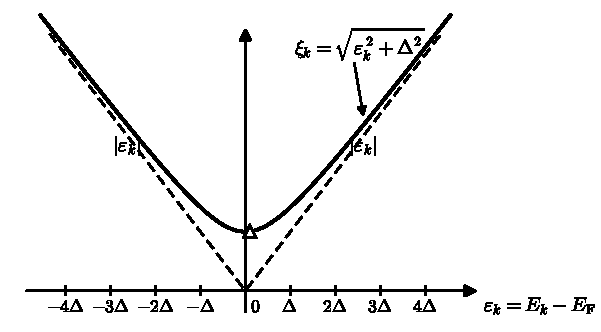
\includegraphics[width=7cm]{fig6-5.pdf}\\{\small 图 6.5\quad 超导体的元激发}
\end{minipage}
\end{center}

下面分别讨论超导能隙，凝聚能，基态和超电流等问题.

\subsection*{1. 能隙$\Delta$的计算}

$T=0$ K时的 $\Delta$，可通过元激发算子 $\alpha_{k}$ 对基态的自洽平均来确定.由于此时无准粒子激发，并且准粒子算符的非对角平均 $\langle\alpha_{-k}\alpha_{k}\rangle=\langle\alpha^{+}_{k}\alpha^{+}_{-k}\rangle=0$，将得到
\begin{equation}
\begin{aligned}
  \Delta&\equiv V\sum_{k}\langle C_{-k}C_{k}\rangle\\
  &=V\sum_{k}\langle0|\left(u_{k}\alpha_{-k}-v_{k}\alpha^{+}_{k}\right)
  \left(u_{k}\alpha_{k}+v_{k}\alpha^{+}_{-k}\right)|0\rangle\\
  &=V\sum_{k}u_{k}v_{k}
\end{aligned}
\end{equation}
利用式(6.4.17)和式(6.4.20)，将上式改写为
\begin{equation}
  \Delta=\frac{1}{2}V\sum_{k}\frac{\Delta}{\xi_{k}}
\end{equation}
当 $\Delta\neq0$ 时，从上式得能隙方程
\begin{equation}
  1=\frac{1}{2}V\sum_{k}\frac{1}{\sqrt{\varepsilon_{k}^{2}+\Delta^{2}}}
\end{equation}
将求和化为积分，并用费密面上一种自旋取向的态密度 $g(0)$ 近似表示吸引区内 $\left(|\varepsilon_{k}|\leqslant\hbar\omega_{\mathrm{D}}\right)$ 的态密度
\begin{equation}
  1=Vg(0)\int_{0}^{\hbar\omega_{\mathrm{D}}}
  \frac{\mathrm{d}\varepsilon}{\sqrt{\varepsilon^{2}+\Delta^{2}}}
\end{equation}
最后求得
\begin{equation}
  \Delta=\frac{\hbar\omega_{\mathrm{D}}}{\sinh\left(\dfrac{1}{g(0)V}\right)}
  \approx 2\hbar\omega_{\mathrm{D}}\exp\Bigl[-\frac{1}{g(0)V}\Bigr]
  \qquad\left[g(0)V\ll1\right]
\end{equation}
对于金属元素，$g(0)V$ 约为 $0.2\sim0.3$，$\hbar\omega_{\mathrm{D}}$ 约为 $10^{-2}$ eV，故能隙 $\Delta$ 约为 $10^{-4}$ eV量级，其具体数据列于表6.1中.

\subsection*{2. 凝聚能$\Delta E(0)$}

根据式(6.4.24)基态能量
\begin{equation}
\begin{aligned}
  E_{\mathrm{s}}&=2\sum_{k}\varepsilon_{k}v_{k}^{2}
  -2\Delta\sum_{k}u_{k}v_{k}+\frac{\Delta^{2}}{V}\\
  &=\sum_{k}\varepsilon_{k}\frac{1}{2}\left(1-\frac{\varepsilon_{k}}{\xi_{k}}\right)
  -2\Delta\sum_{k}\frac{1}{2}\frac{\Delta}{\xi_{k}}
  +\frac{\Delta^{2}}{2}\sum_{k}\frac{1}{\xi_{k}}\\
  &=\sum_{k}\varepsilon_{k}-\sum_{k}\frac{\varepsilon_{k}^{2}}{\xi_{k}}
  -\frac{1}{2}\Delta^{2}\sum_{k}\frac{1}{\xi_{k}}\\
  &=\sum_{k}\left(\varepsilon_{k}
  -\frac{2\varepsilon_{k}^{2}+\Delta^{2}}{2\xi_{k}}\right)
\end{aligned}
\end{equation}
其中还利用了式(6.4.25)和式(6.4.27). $E_{\mathrm{s}}(0)$ 与正常态费密球分布能量 $E_{\mathrm{n}}(0)=\sum_{k<k_{\mathrm{F}}}2\varepsilon_{k}$ 之差代表凝聚能，即
\begin{equation}
\begin{aligned}
  E_{\mathrm{s}}(0)-E_{\mathrm{n}}(0)
  &=\sum_{k>k_{\mathrm{F}}}\left(\varepsilon_{k}
  -\frac{2\varepsilon_{k}^{2}+\Delta^{2}}{2\xi_{k}}\right)
  +\sum_{k<k_{\mathrm{F}}}\left(-\varepsilon_{k}
  -\frac{2\varepsilon_{k}^{2}+\Delta^{2}}{2\xi_{k}}\right)\\
  &=2\sum_{k>k_{\mathrm{F}}}\left(\varepsilon_{k}
  -\frac{2\varepsilon_{k}^{2}+\Delta^{2}}{2\xi_{k}}\right)
  \quad\text{（因为电子-空穴对称性）}\\
  &=2g(0)\int_{0}^{\hbar\omega_{\mathrm{D}}}
  \left(\varepsilon-\frac{2\varepsilon^{2}+\Delta^{2}}
  {2\sqrt{\varepsilon^{2}+\Delta^{2}}}\right)\mathrm{d}\varepsilon\\
  &=g(0)\left(\hbar\omega_{\mathrm{D}}\right)^{2}
  \left[1-\sqrt{1+\left(\frac{\Delta}{\hbar\omega_{\mathrm{D}}}\right)^{2}}\right]\\
  &\approx-\frac{1}{2}g(0)\Delta^{2}
  \quad\text{（因为}\ \hbar\omega_{\mathrm{D}}\gg\Delta\text{）}
\end{aligned}
\end{equation}
上式表明凝聚能为负，说明超导基态能量低于正常态能量，因此必然发生超导相变.换句话说，只要存在能隙，就会有一个比费密球态能量更低的超导态出现，即超导是一种凝聚态.

\subsection*{3. BCS基态}

超导基态应当是准粒子消灭算符 $\alpha_{k}$ 与 $\alpha_{-k}$ 的真空态，并满足条件
\begin{equation}
  \alpha_{k}|0\rangle=\alpha_{-k}|0\rangle=0
\end{equation}
不难验证，态
\begin{equation}
  \prod_{k}\alpha_{k}\alpha_{-k}|\mathrm{Vac}\rangle
\end{equation}
满足基态条件式(6.4.32)，因为从反对易式 $\left[\alpha_{k},\alpha_{k}\right]_{+}=0$，可得算符恒等式
\begin{equation}
  \alpha_{k}\alpha_{k}\equiv0
\end{equation}
因此
\begin{equation*}
  \alpha_{k'}\prod_{k}\alpha_{k}\alpha_{-k}|\mathrm{Vac}\rangle
  =\left(\alpha_{k'}\alpha_{k'}\right)\alpha_{-k'}
  \prod_{k\neq k'}\alpha_{k}\alpha_{-k}|\mathrm{Vac}\rangle=0
\end{equation*}
类似的，有
\begin{equation*}
  \alpha_{-k'}\prod_{k}\alpha_{k}\alpha_{-k}|\mathrm{Vac}\rangle
  =-\left(\alpha_{-k'}\alpha_{-k'}\right)\alpha_{k'}
  \prod_{k\neq k'}\alpha_{k}\alpha_{-k}|\mathrm{Vac}\rangle=0
\end{equation*}
将变换公式(6.4.9)代入式(6.4.33)得
\begin{equation}
\begin{aligned}
  \prod_{k}\alpha_{k}\alpha_{-k}|\mathrm{Vac}\rangle
  &=\prod_{k}\left(u_{k}C_{k}-v_{k}C^{+}_{-k}\right)
  \left(u_{k}C_{-k}+v_{k}C^{+}_{k}\right)|\mathrm{Vac}\rangle\\
  &=\prod_{k}\left(u_{k}v_{k}C_{k}C^{+}_{k}
  +v_{k}^{2}C^{+}_{k}C^{+}_{-k}\right)|\mathrm{Vac}\rangle\\
  &=\prod_{k}\left(u_{k}v_{k}
  +v_{k}^{2}C^{+}_{k}C^{+}_{-k}\right)|\mathrm{Vac}\rangle
\end{aligned}
\end{equation}
其中 $|\mathrm{Vac}\rangle$ 为真正的真空态，$C_{k}|\mathrm{Vac}\rangle=C_{-k}|\mathrm{Vac}\rangle=0$，$C_{k}C^{+}_{k}|\mathrm{Vac}\rangle=|\mathrm{Vac}\rangle$.对于正常态 $\Delta=0$，根据式(6.4.21) $u_{k}v_{k}=0$，$v_{k}^{2}$ 在费密球内等于1，在球外为零.此时式(6.4.35)变为正常相的费密球分布态：
\begin{equation}
  |F\rangle=\prod_{k<k_{\mathrm{F}}}C^{+}_{k}C^{+}_{-k}|\mathrm{Vac}\rangle
\end{equation}
若将式(6.4.35)归一，由于
\begin{equation}
\begin{aligned}
  &\langle\mathrm{Vac}|\prod_{k}\left(u_{k}v_{k}+v_{k}^{2}C_{-k}C_{k}\right)
  \left(u_{k}v_{k}+v_{k}^{2}C^{+}_{k}C^{+}_{-k}\right)|\mathrm{Vac}\rangle\\
  &\quad=\langle\mathrm{Vac}|\prod_{k}\left(u_{k}^{2}v_{k}^{2}
  +v_{k}^{4}C_{-k}C_{k}C^{+}_{k}C^{+}_{-k}\right)|\mathrm{Vac}\rangle\\
  &\quad=\prod_{k}\left(u_{k}^{2}v_{k}^{2}+v_{k}^{4}\right)
  =\prod_{k}v_{k}^{2}=\Bigl(\prod_{k}v_{k}\Bigr)^{2}
\end{aligned}
\end{equation}
可以取 $\prod_{k}v_{k}$ 为归一化常数.因此，归一化的基态为
\begin{equation}
\begin{aligned}
  |0\rangle&=\frac{1}{\bigl(\prod_{k}v_{k}\bigr)}
  \prod_{k}\left(u_{k}v_{k}+v_{k}^{2}C^{+}_{k}C^{+}_{-k}\right)
  |\mathrm{Vac}\rangle\\
  &=\prod_{k}\left(u_{k}+v_{k}C^{+}_{k}C^{+}_{-k}\right)|\mathrm{Vac}\rangle
\end{aligned}
\end{equation}
与BCS的超导基态式(6.4.1)一致，可认为是BCS假定的证明，并且 $u_{k}$ 与 $v_{k}$ 均已求出.

若对电子的占据数算符 $C^{+}_{k}C_{k}$ 求基态平均，可得
\begin{equation*}
\begin{aligned}
  \langle0|C^{+}_{k}C_{k}|0\rangle
  &=\langle0|\left(u_{k}\alpha^{+}_{k}+v_{k}\alpha_{-k}\right)
  \left(u_{k}\alpha_{k}+v_{k}\alpha^{+}_{-k}\right)|0\rangle\\
  &=v_{k}^{2}\langle0|\alpha_{-k}\alpha^{+}_{-k}|0\rangle=v_{k}^{2}
\end{aligned}
\end{equation*}
显然，$v_{k}^{2}$ 代表被占据概率，它与正常态分布的差别主要在费密面附近 $2\Delta$ 宽度内，如图6.6所示.图6.6中 $v_{k}^{2}$ 曲线和有限温度的费密分布相似，但应注意现在是 $T=0$ K情况，费密面的"模糊化"是由于形成了库柏对.库柏对的零温分布由
\begin{equation}
  \langle0|C_{-k}C_{k}|0\rangle=u_{k}v_{k}
  =\frac{1}{2}\Delta/\sqrt{\left(E_{k}-E_{\mathrm{F}}\right)^{2}+\Delta^{2}}
\end{equation}
决定.显然，库柏对的凝聚主要发生在费密能 $E_{\mathrm{F}}$ 附近.

\begin{center}
\begin{minipage}{5.5cm}
\centering
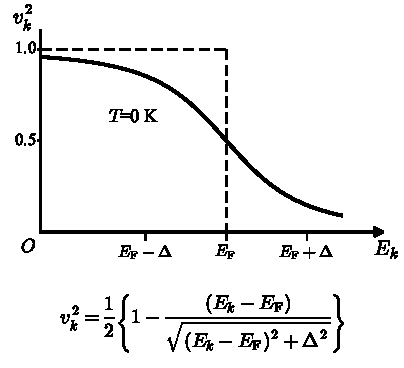
\includegraphics[width=5.5cm]{fig6-6.pdf}\\{\small 图 6.6\quad 超导体中的零温粒子分布}
\end{minipage}
\end{center}

\subsection*{4. 超导体中的元激发}

从BCS超导体的对角化哈密顿量
\begin{equation*}
  \overline{H}=E_{\mathrm{s}}
  +\sum_{k}\xi_{k}\left(\alpha^{+}_{k}\alpha_{k}
  +\alpha^{+}_{-k}\alpha_{-k}\right)
\end{equation*}
可知，对于单准粒子激发态
\begin{equation}
  |1_{k}\rangle=\alpha^{+}_{k}|0\rangle
\end{equation}
其元激发能量为
\begin{equation}
  \langle1_{k}|\overline{H}|1_{k}\rangle
  -\langle0|\overline{H}|0\rangle=\xi_{k}
  =\sqrt{\varepsilon_{k}^{2}+\Delta^{2}}
\end{equation}
在费密面上 $\varepsilon_{k}=\varepsilon_{\mathrm{F}}=0$，这时
\begin{equation}
  \xi_{k}=\xi_{\mathrm{F}}=\Delta
\end{equation}
$\Delta$ 是单个准粒子激发所需的最小能量，而任意k的单准粒子激发能为 $\xi_{k}$.由于准粒子算符 $\alpha^{+}_{k}=u_{k}C^{+}_{k}-v_{k}C_{-k}$ 代表电子与空穴的混合，因此既存在"电子"型也存在"空穴"型的准粒子激发.当元激发使系统总粒子数从 $N\to N+1$ 时，超导体中产生"电子"型元激发，而当 $N\to N-1$ 时，产生"空穴"型激发，它们所需的最小能量都是 $\Delta$.实验上可以通过超导体(S)与正常金属(N)的隧道效应，注入电子或空穴，形成"电子"型或"空穴"型元激发.

现在作图像说明\textsuperscript{[3]}：首先考虑超导态是费密面附近电子形成库柏对，并近似认为这些对大致分布在化学势 $\mu$（或费密能 $E_{\mathrm{F}}$）上，由于超导体中准粒子激发能为 $\xi_{k}$，相对于 $\mu$（或 $E_{\mathrm{F}}$）作 $\xi_{k}$ 曲线，如图6.7所示，它可以作为说明超导元激发的图像.图6.8是正常金属与超导体N-S接触的能谱图像，其中(a)为偏压 $V=0$ 情况，这时N-S结两边化学势相等，而(b)为加正向偏压情况.当 $eV\geqslant\Delta$ 时可从N向S注入电子产生"电子型"元激发，若加反向偏压［如图(c)］，则只有当 $e|V|\geqslant\Delta$ 时，超导体中取出一个电子所得到的能量才足够使剩下的配偶电子激发到 $\xi_{k}$ 曲线上去，这就是注入空穴情况.因此，"电子"型或"空穴"型激发所需最小能量都是 $\Delta$.

\begin{center}
\begin{minipage}{5cm}
\centering
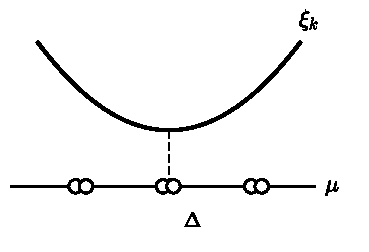
\includegraphics[width=5cm]{fig6-7.pdf}\\{\small 图 6.7\quad 超导体的BCS模型}
\end{minipage}
\end{center}

\begin{center}
\begin{minipage}{8cm}
\centering
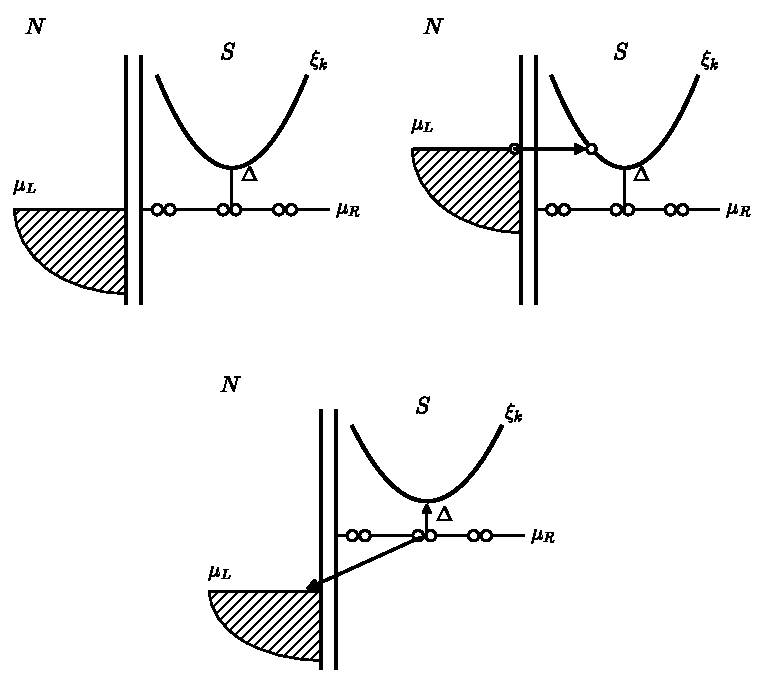
\includegraphics[width=8cm]{fig6-8.pdf}\\[0.3em]
{\small (a) 偏压 $V=0$\qquad\qquad (b) 注入电子 $eV\geqslant\Delta$}\\[0.2em]
{\small (c) 注入空穴 $e|V|\geqslant\Delta$}\\[0.2em]
{\small 图 6.8\quad 超导与正常金属接触}
\end{minipage}
\end{center}

假如在费密面以下激发一个粒子到费密面以上，保持系统总粒子数不变.这时相当于产生了两个准粒子激发，一个是"空穴"型的，一个是"电子"型的.所需最小能量为 $2\Delta$，如图6.9所示，称为电子-空穴对型激发，它相当于拆开一个库柏对.在BCS理论中，电子-空穴对型激发为
\begin{equation}
  \alpha^{+}_{k}\alpha^{+}_{-k}|0\rangle\equiv|\text{对}\rangle
\end{equation}
其元激发能量等于
\begin{equation}
\begin{aligned}
  &\langle\text{对}|\overline{H}|\text{对}\rangle
  -\langle0|\overline{H}|0\rangle\\
  &\quad=\sum_{k'}\xi_{k'}\langle0|\alpha_{-k}\alpha_{k}
  \left(\alpha^{+}_{k'}\alpha_{k'}
  +\alpha^{+}_{-k'}\alpha_{-k'}\right)\alpha^{+}_{k}\alpha^{+}_{-k}|0\rangle
  =2\xi_{k}
\end{aligned}
\end{equation}
同样也说明最小激发能为 $2\Delta$.

\begin{center}
\begin{minipage}{5cm}
\centering
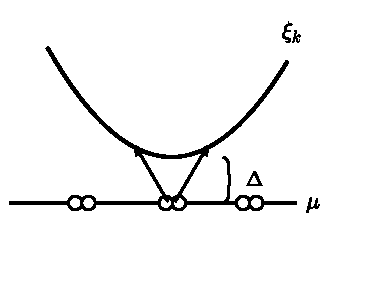
\includegraphics[width=5cm]{fig6-9.pdf}\\{\small 图 6.9\quad 电子-空穴对型激发}
\end{minipage}
\end{center}

\subsection*{5. 超电流}

以上所讨论只是不载流的超导态情况，其中每个库柏对为 $(\boldsymbol{k}\uparrow,-\boldsymbol{k}\downarrow)$，其总动量为 $\hbar\boldsymbol{K}=\hbar\boldsymbol{k}+\hbar(-\boldsymbol{k})=0$，如图6.10(a).由于外场作用将使费密球移动 $\delta\boldsymbol{k}$，相应的库柏对变为 $(\boldsymbol{k}+\delta\boldsymbol{k}\uparrow,-\boldsymbol{k}+\delta\boldsymbol{k}\downarrow)$，其总动量等于 $\hbar(2\delta\boldsymbol{k})$，质心速度为 $\dfrac{\hbar\delta\boldsymbol{k}}{m}$，如图6.10(b)，称为载流超导态.因此库柏对运动的电流密度为
\begin{equation}
  j_{\mathrm{s}}=\frac{n}{2}(-2e)\frac{\hbar\delta k}{m}
  =-\frac{ne\hbar\delta k}{m}
\end{equation}

\begin{center}
\begin{minipage}{9cm}
\centering
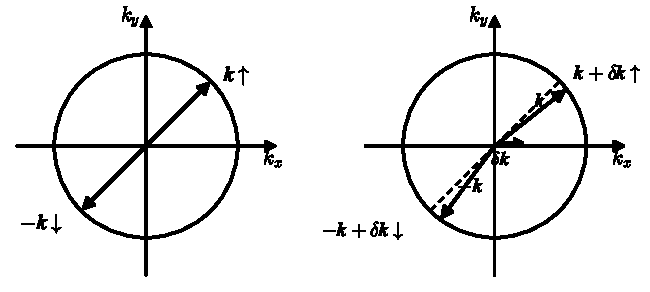
\includegraphics[width=9cm]{fig6-10.pdf}\\[0.3em]
{\small (a) 超导基态\qquad\qquad (b) 载流超导态}\\[0.2em]
{\small 图 6.10\quad 载流超导体中的库柏对}
\end{minipage}
\end{center}

由于互作用只使 $(\boldsymbol{k}+\delta\boldsymbol{k}\uparrow,-\boldsymbol{k}+\delta\boldsymbol{k}\downarrow)$ 库柏对散射为 $(\boldsymbol{k}'+\delta\boldsymbol{k}\uparrow,-\boldsymbol{k}'+\delta\boldsymbol{k}\downarrow)$ 库柏对，总动量不变，即使外场撤去，超导体中仍保持图6.10(b)的组态，因此超导电流 $j_{\mathrm{s}}$ 将不衰减，这说明库柏对所载电流是无阻电流.

$j_{\mathrm{s}}$ 存在一个上限，因为费密球位移 $\delta\boldsymbol{k}$ 将引起动能增加
\begin{equation*}
  \delta\mathcal{E}\approx\left(\frac{n}{2}\right)\frac{1}{2}(2m)
  \left(\frac{\hbar\delta k}{m}\right)^{2}
  =\frac{n\hbar^{2}(\delta k)^{2}}{2m}
\end{equation*}
当 $\delta\mathcal{E}$ 大于凝聚能 $\dfrac{1}{2}g(0)\Delta^{2}$ 时，超导相不再是稳定的，库柏对将被拆散成为正常态，而有电阻，$\delta k$ 的临界值可根据 $\dfrac{n\hbar^{2}(\delta k)_{\mathrm{c}}^{2}}{2m}=\dfrac{1}{2}g(0)\Delta^{2}$ 估计
\begin{equation*}
  |\delta k|_{\mathrm{c}}=\sqrt{\frac{mg(0)}{n}}\left(\frac{\Delta}{\hbar}\right)
  =\sqrt{\frac{3m}{4E_{\mathrm{F}}}}\left(\frac{\Delta}{\hbar}\right)
  \approx\frac{m\Delta}{\hbar^{2}k_{\mathrm{F}}}
\end{equation*}
其中 $g(0)=\dfrac{3n}{4E_{\mathrm{F}}}$.因此，超导电流密度的上限
\begin{equation}
  j_{\mathrm{c}}=\frac{ne\hbar}{m}|\delta k_{\mathrm{c}}|
  \approx\frac{ne\Delta}{\hbar k_{\mathrm{F}}}
\end{equation}
$j_{\mathrm{c}}$ 称为临界电流密度，约为 $10^{7}\,\mathrm{A\,cm^{-2}}$ 量级.这是超导体所能载送的最大电流密度，超导电流满足条件
\begin{equation}
  j_{\mathrm{s}}<\frac{ne}{\hbar k_{\mathrm{F}}}\Delta
\end{equation}
因此，超导体中的无阻电流和能隙的存在直接有关.产生电阻并使 $j_{\mathrm{s}}$ 衰减的弛豫过程，对应于在图6.10(b)中费密球右边留下空穴，而在左边产生电子，相当于从超导态产生两个单粒子型的激发（一个空穴，一个电子），它至少必须有 $2\Delta$ 的能量.当库柏对在外场驱动下的动能 $\dfrac{\hbar k_{\mathrm{F}}}{m}\hbar(2\delta k)<2\Delta$ 时，上述弛豫过程在能量上是不利的，因此不可能发生，这时将得到条件
\begin{equation*}
  \delta k<\frac{m\Delta}{\hbar^{2}k_{\mathrm{F}}}\approx|\delta k_{\mathrm{c}}|
\end{equation*}
它就是
\begin{equation*}
  j_{\mathrm{s}}=\frac{ne\hbar\delta k}{m}
  <\frac{ne\hbar}{m}\frac{m\Delta}{\hbar^{2}k_{\mathrm{F}}}
  =\frac{ne\Delta}{\hbar k_{\mathrm{F}}}
\end{equation*}
以上是BCS理论对超电流的微观解释.这一简单论证不适用于无能隙超导体，其详细讨论见\textsuperscript{[4]}.

\section{有限温度情况}

$T>0$ K时，式(6.4.5)中 $\langle\cdots\rangle$ 代表统计平均 $\langle\cdots\rangle_{T}$，这时存在准粒子的热激发 $\langle\alpha^{+}_{k}\alpha_{k}\rangle_{T}$.因此，有限温度的能隙方程为
\begin{equation}
\begin{aligned}
  \Delta(T)&=V\sum_{k}\langle C_{-k}C_{k}\rangle_{T}\\
  &=V\sum_{k}\langle\left(u_{k}\alpha_{-k}-v_{k}\alpha^{+}_{k}\right)
  \left(u_{k}\alpha_{k}+v_{k}\alpha^{+}_{-k}\right)\rangle_{T}\\
  &=V\sum_{k}u_{k}v_{k}\left(\langle\alpha_{-k}\alpha^{+}_{-k}\rangle_{T}
  -\langle\alpha^{+}_{k}\alpha_{k}\rangle_{T}\right)\\
  &=V\sum_{k}u_{k}v_{k}\left(1-\langle\alpha^{+}_{k}\alpha_{k}\rangle_{T}
  -\langle\alpha^{+}_{-k}\alpha_{-k}\rangle_{T}\right)
\end{aligned}
\end{equation}
由于哈密顿量［式(6.4.23)］已表示为费密算子 $\alpha_{k}$ 的对角形式，$\overline{H}$ 是以 $\xi_{k}$ 为元激发能量的无相互作用准粒子系统.准粒子应当满足费密分布.
\begin{equation}
  \langle\alpha^{+}_{-k}\alpha_{-k}\rangle_{T}
  =\langle\alpha^{+}_{k}\alpha_{k}\rangle_{T}=f(\xi_{k})
  =\left[\exp\left(\frac{\xi_{k}}{k_{\mathrm{B}}T}\right)+1\right]^{-1}
\end{equation}
其中
\begin{equation}
  \xi_{k}=\sqrt{\varepsilon_{k}^{2}+\Delta^{2}(T)}
\end{equation}
$\Delta(T)$ 满足方程
\begin{equation}
  \Delta(T)=V\sum_{k}u_{k}v_{k}\left\{1-2f(\xi_{k})\right\}
\end{equation}
变换系数 $u_{k}$ 与 $v_{k}$ 的形式仍与式(6.4.20)相同，只是其中的 $\Delta=\Delta(0)$ 换成了 $\Delta(T)$
\begin{equation}
  \left.
  \begin{aligned}
    &u_{k}^{2}=\frac{1}{2}\left(1+\frac{\varepsilon_{k}}
    {\sqrt{\varepsilon_{k}^{2}+\Delta^{2}(T)}}\right)\\
    &v_{k}^{2}=\frac{1}{2}\left(1-\frac{\varepsilon_{k}}
    {\sqrt{\varepsilon_{k}^{2}+\Delta^{2}(T)}}\right)
  \end{aligned}\right\}
\end{equation}
将式(6.5.5)代入式(6.5.4)消去 $\Delta(T)$ 因子，求得有限温度的能隙方程为
\begin{equation}
\begin{aligned}
  1&=\frac{1}{2}V\sum_{k}\frac{1-2f(\xi_{k})}{\xi_{k}}\\
  &=\frac{1}{2}V\sum_{k}\frac{\tanh\left(\frac{1}{2}\beta\xi_{k}\right)}{\xi_{k}}
  \qquad\left(\beta=\frac{1}{k_{\mathrm{B}}T}\right)
\end{aligned}
\end{equation}
由式(6.5.6)可以确定能隙与温度关系以及超导转变温度 $T_{\mathrm{c}}$.对于热力学量如熵和比热容等的计算，式(6.5.6)也是必须的自洽条件.

\subsection*{1. 确定$T_{\mathrm{c}}$}

由于 $\Delta(T)\to0$ 时 $\xi_{k}\to|\varepsilon_{k}|$，超导元激发变为正常电子的激发，因此超导正常转变温度 $T_{\mathrm{c}}$ 由条件
\begin{equation}
  \Delta(T_{\mathrm{c}})=0
\end{equation}
决定. $T=T_{\mathrm{c}}$ 时式(6.5.6)可写成
\begin{equation*}
\begin{aligned}
  1&=g(0)V\int_{0}^{\hbar\omega_{\mathrm{D}}}\mathrm{d}\varepsilon\,
  \frac{\tanh\left(\frac{1}{2}\beta_{\mathrm{c}}\varepsilon\right)}{\varepsilon}\\
  &=g(0)V\int_{0}^{\frac{1}{2}\beta_{\mathrm{c}}\hbar\omega_{\mathrm{D}}}
  \mathrm{d}x\,\frac{\tanh x}{x}
\end{aligned}
\end{equation*}
作分部积分
\begin{equation*}
  1=g(0)V\left\{\ln x\tanh x\Bigl|
  _{0}^{\frac{1}{2}\beta_{\mathrm{c}}\hbar\omega_{\mathrm{D}}}
  -\int_{0}^{\frac{1}{2}\beta_{\mathrm{c}}\hbar\omega_{\mathrm{D}}}
  \mathrm{d}x\,\ln x\,\mathrm{sech}^{2}x\right\}
\end{equation*}
其中 $\beta_{\mathrm{c}}=\left(k_{\mathrm{B}}T_{\mathrm{c}}\right)^{-1}$.由于积分是收敛的，并且 $\hbar\omega_{\mathrm{D}}\gg k_{\mathrm{B}}T$，积分的上限可换为 $\infty$，上式可近似为
\begin{equation}
  1=g(0)V\left\{\ln\left(\frac{\hbar\omega_{\mathrm{D}}}{2k_{\mathrm{B}}T_{\mathrm{c}}}\right)
  -\int_{0}^{\infty}\mathrm{d}x\,\ln x\,\mathrm{sech}^{2}x\right\}
\end{equation}
利用欧拉（Euler）积分公式
\begin{equation*}
  \int_{0}^{\infty}\mathrm{d}x\,\ln x\,\mathrm{sech}^{2}x
  =-\ln\frac{4\mathrm{e}^{\gamma}}{\pi}
\end{equation*}
其中 $\gamma\approx0.5772$ 是欧拉常数，$\dfrac{2\mathrm{e}^{\gamma}}{\pi}\approx1.13$，可把式(6.5.8)简化为
\begin{equation}
  1=g(0)V\ln\left[\left(\frac{2\mathrm{e}^{\gamma}}{\pi}\right)
  \left(\frac{\hbar\omega_{\mathrm{D}}}{k_{\mathrm{B}}T_{\mathrm{c}}}\right)\right]
\end{equation}
从而求得
\begin{equation}
\begin{aligned}
  k_{\mathrm{B}}T_{\mathrm{c}}&=\frac{2\mathrm{e}^{\gamma}}{\pi}
  \hbar\omega_{\mathrm{D}}\exp\Bigl[-\frac{1}{g(0)V}\Bigr]\\
  &\approx 1.13\,\hbar\omega_{\mathrm{D}}
  \exp\Bigl[-\frac{1}{g(0)V}\Bigr]
\end{aligned}
\end{equation}
上式与零温能隙公式(6.4.29)相比较，得到BCS超导体的一个普适关系式
\begin{equation}
  \frac{2\Delta(0)}{k_{\mathrm{B}}T_{\mathrm{c}}}=2\pi\mathrm{e}^{-\gamma}
  \approx 3.53
\end{equation}
$2\pi\mathrm{e}^{-\gamma}$ 是与材料特性无关的常数.除Pb以外，这个结果与实验基本符合，如表6.1所示.

由于声子的德拜频率 $\omega_{\mathrm{D}}\sim M^{-1/2}$，M为金属离子质量，则式(6.5.10)给出 $T_{\mathrm{c}}M^{\frac{1}{2}}=$ 常数的同位素效应公式.

\subsection*{2. 能隙与温度关系}

为了求得 $\Delta(T)$，应求下列积分方程的数值解：
\begin{equation}
\begin{aligned}
  1&=\frac{1}{2}V\sum_{k}\frac{1}{\sqrt{\varepsilon_{k}^{2}+\Delta^{2}(T)}}
  -V\sum_{k}\frac{1}{\sqrt{\varepsilon_{k}^{2}+\Delta^{2}(T)}}\times\\
  &\quad\left[\exp\bigl(\beta\sqrt{\varepsilon_{k}^{2}+\Delta^{2}(T)}\bigr)+1\right]^{-1}
\end{aligned}
\end{equation}
当 $T\to0$ 时，$\{\cdots\}^{-1}\to0$，上式变为
\begin{equation}
\begin{aligned}
  1&=\frac{1}{2}V\sum_{k}\frac{1}{\sqrt{\varepsilon_{k}^{2}+\Delta^{2}(T)}}
  =g(0)V\,\mathrm{arsinh}\,\frac{\hbar\omega_{\mathrm{D}}}{\Delta(0)}\\
  &\approx g(0)V\ln\frac{2\hbar\omega_{\mathrm{D}}}{\Delta(0)}
\end{aligned}
\end{equation}
求得的 $\Delta(0)$ 与式(6.4.28)一致.

式(6.5.12)右边第一项可改写成
\begin{equation*}
  g(0)V\ln\frac{2\hbar\omega_{\mathrm{D}}}{\Delta(T)}
\end{equation*}
再利用式(6.5.13)将积分方程(6.5.12)表示为
\begin{equation}
\begin{aligned}
  \ln\left[\frac{\Delta(0)}{\Delta(T)}\right]
  &=2\int_{0}^{\hbar\omega_{\mathrm{D}}}
  \frac{\mathrm{d}\varepsilon}{\sqrt{\varepsilon^{2}+\Delta^{2}(T)}}\times\\
  &\quad\frac{1}{\left[\exp\bigl(\beta\sqrt{\varepsilon^{2}+\Delta^{2}(T)}\bigr)+1\right]}
\end{aligned}
\end{equation}
上式表明随着温度升高 $\Delta(T)$ 单调减小.由于 $\hbar\omega_{\mathrm{D}}\gg k_{\mathrm{B}}T$（$0\leqslant T\leqslant T_{\mathrm{c}}$），存在着近似关系式
\begin{equation}
\begin{aligned}
  \ln\left[\frac{\Delta(T)}{\Delta(0)}\right]
  &=-2\int_{0}^{\infty}\mathrm{d}x\,
  \frac{1}{\sqrt{x^{2}+\left(\dfrac{\Delta(T)}{k_{\mathrm{B}}T}\right)^{2}}}\times\\
  &\quad\frac{1}{\left[\exp\sqrt{x^{2}+\left(\dfrac{\Delta(T)}{k_{\mathrm{B}}T}\right)^{2}}\right]+1}
\end{aligned}
\end{equation}
因此 $\dfrac{\Delta(T)}{\Delta(0)}$ 是 $\dfrac{k_{\mathrm{B}}T}{\Delta(0)}$ 或 $\dfrac{T}{T_{\mathrm{c}}}$ 的普适函数，其数值计算结果如图6.11，与实验测量相符.

\begin{center}
\begin{minipage}{6.5cm}
\centering
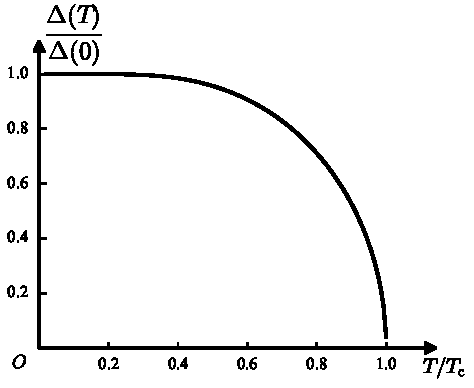
\includegraphics[width=6.5cm]{fig6-11.pdf}\\{\small 图 6.11\quad 能隙与温度关系}
\end{minipage}
\end{center}

当 $T\ll T_{\mathrm{c}}$ 时，由于 $\Delta(T)\approx\Delta(0)$，式(6.5.14)可写成
\begin{equation*}
  \ln\left[\frac{\Delta(T)}{\Delta(0)}\right]
  =-2\int_{0}^{\hbar\omega_{\mathrm{D}}}\mathrm{d}\varepsilon\,
  \frac{\exp\bigl[-\beta\sqrt{\varepsilon^{2}+\Delta^{2}(0)}\bigr]}
  {\sqrt{\varepsilon^{2}+\Delta^{2}(0)}}
\end{equation*}
考虑到 $\beta\Delta(0)\gg1$，积分中指数因子迅速衰减，故 $\varepsilon\approx0$ 对积分贡献最大.这时 $\sqrt{\varepsilon^{2}+\Delta^{2}(0)}$ 可按照 $\dfrac{\varepsilon}{\Delta(0)}$ 展开，其近似结果为
\begin{equation}
\begin{aligned}
  \ln\left[\frac{\Delta(T)}{\Delta(0)}\right]
  &=-\frac{2}{\Delta(0)}\int_{0}^{\hbar\omega_{\mathrm{D}}}\mathrm{d}\varepsilon\,
  \mathrm{e}^{-\frac{\Delta(0)}{k_{\mathrm{B}}T}
  \left(1+\frac{\varepsilon^{2}}{2\Delta^{2}(0)}\right)}\\
  &=-\frac{2}{\Delta(0)}\left[2k_{\mathrm{B}}T\Delta(0)\right]^{1/2}
  \mathrm{e}^{-\frac{\Delta(0)}{k_{\mathrm{B}}T}}
  \int_{0}^{\infty}\mathrm{d}x\,\mathrm{e}^{-x^{2}}\\
  &=-\left(\frac{2\pi k_{\mathrm{B}}T}{\Delta(0)}\right)^{1/2}
  \mathrm{e}^{-\frac{\Delta(0)}{k_{\mathrm{B}}T}}
\end{aligned}
\end{equation}
又因为 $T\ll T_{\mathrm{c}}$ 时，$\Delta(0)-\Delta(T)\ll\Delta(0)$，因此有
\begin{equation*}
  \ln\frac{\Delta(T)}{\Delta(0)}
  =\ln\left(1-\frac{\Delta(0)-\Delta(T)}{\Delta(0)}\right)
  \approx\frac{\Delta(T)-\Delta(0)}{\Delta(0)}
\end{equation*}
可求得 $\Delta(T)$ 的低温近似式
\begin{equation}
  \Delta(T)\approx\Delta(0)-\left[2\pi k_{\mathrm{B}}T\Delta(0)\right]^{1/2}
  \mathrm{e}^{-\frac{\Delta(0)}{k_{\mathrm{B}}T}}
  \qquad(T\ll T_{\mathrm{c}})
\end{equation}
为导出 $T\to T_{\mathrm{c}}$ 时能隙 $\Delta(T)$ 的近似式，最好从自洽方程(6.5.6)出发
\begin{equation}
\begin{aligned}
  1&=g(0)V\int_{0}^{\hbar\omega_{\mathrm{D}}}
  \frac{\tanh\left(\frac{1}{2}\beta\xi\right)}{\xi}\,\mathrm{d}\varepsilon\\
  &=g(0)V\int_{0}^{\hbar\omega_{\mathrm{D}}}
  \frac{f(-\xi)-f(\xi)}{\xi}\,\mathrm{d}\varepsilon
\end{aligned}
\end{equation}
利用泊松求和公式\footnote{详见附录E.}
\begin{equation}
\begin{aligned}
  f(\xi)&=k_{\mathrm{B}}T\sum_{n=-\infty}^{\infty}
  \frac{\mathrm{e}^{\mathrm{i}\omega_{n}\eta}}{\mathrm{i}\omega_{n}-\xi}\\
  \omega_{n}&=(2n+1)\pi k_{\mathrm{B}}T\qquad(n=\text{整数})
\end{aligned}
\end{equation}
并令 $\eta\to+0$，求得
\begin{equation}
  \frac{\tanh\left(\frac{1}{2}\beta\varepsilon\right)}{\varepsilon}
  =\frac{f(-\varepsilon)-f(\varepsilon)}{\varepsilon}
  =4k_{\mathrm{B}}T\sum_{n=0}^{\infty}
  \frac{1}{\omega_{n}^{2}+\varepsilon^{2}+\Delta^{2}(T)}
\end{equation}
代入式(6.5.18)，将自洽方程用下列级数的积分表示：
\begin{equation}
  1=4k_{\mathrm{B}}Tg(0)V\int_{0}^{\hbar\omega_{\mathrm{D}}}\mathrm{d}\varepsilon
  \sum_{n=0}^{\infty}
  \frac{1}{\omega_{n}^{2}+\varepsilon^{2}+\Delta^{2}(T)}
\end{equation}
用上式便于求近似.由于 $T\to T_{\mathrm{c}}$ 时 $\Delta(T)\to0$，可令 $\Delta$ 为小参量，并将上式按 $\Delta(T)$ 展开，得
\begin{equation}
\begin{aligned}
  1&=4k_{\mathrm{B}}Tg(0)V\sum_{n=0}^{\infty}\int_{0}^{\hbar\omega_{\mathrm{D}}}
  \mathrm{d}\varepsilon\left\{\frac{1}{\left(\omega_{n}^{2}+\varepsilon^{2}\right)}
  -\frac{\Delta^{2}(T)}{\left(\omega_{n}^{2}+\varepsilon^{2}\right)^{2}}+\cdots\right\}\\
  &=g(0)V\left\{\int_{0}^{\hbar\omega_{\mathrm{D}}}\mathrm{d}\varepsilon\,
  \frac{\tanh\left(\frac{1}{2}\beta\varepsilon\right)}{\varepsilon}
  -4k_{\mathrm{B}}T\Delta^{2}(T)\sum_{n=0}^{\infty}
  \int_{0}^{\hbar\omega_{\mathrm{D}}}
  \frac{\mathrm{d}\varepsilon}{\left(\omega_{n}^{2}+\varepsilon^{2}\right)^{2}}\right\}
\end{aligned}
\end{equation}
利用欧拉积分，求得式中的
\begin{equation}
  \int_{0}^{\hbar\omega_{\mathrm{D}}}\mathrm{d}\varepsilon\,
  \frac{\tanh\left(\frac{1}{2}\beta\varepsilon\right)}{\varepsilon}
  =\ln\left[\left(\frac{2\mathrm{e}^{\gamma}}{\pi}\right)
  \left(\frac{\hbar\omega_{\mathrm{D}}}{k_{\mathrm{B}}T}\right)\right]
\end{equation}
再根据式(6.5.9)将式(6.5.22)写成
\begin{equation}
\begin{aligned}
  \ln\left(\frac{T}{T_{\mathrm{c}}}\right)
  &=-4k_{\mathrm{B}}T\Delta^{2}(T)\sum_{n=0}^{\infty}
  \int_{0}^{\hbar\omega_{\mathrm{D}}}\mathrm{d}\varepsilon\,
  \frac{1}{\left(\omega_{n}^{2}+\varepsilon^{2}\right)^{2}}\\
  &\approx-\left[\frac{\Delta(T)}{\pi k_{\mathrm{B}}T}\right]^{2}
  \sum_{n=0}^{\infty}\frac{1}{(2n+1)^{3}}
\end{aligned}
\end{equation}
等式右边的级数可用黎曼 $\zeta$ 函数表示，因为
\begin{equation}
  \sum_{n=0}^{\infty}\frac{1}{(2n+1)^{3}}=\frac{7}{8}\zeta(3)
\end{equation}
其中 $\zeta(3)=1.202$ 是黎曼 $\zeta$ 函数.当 $T_{\mathrm{c}}-T\ll T_{\mathrm{c}}$ 时，有下列近似关系：
\begin{equation}
  \ln\left(\frac{T}{T_{\mathrm{c}}}\right)
  =\ln\left(1+\frac{T-T_{\mathrm{c}}}{T_{\mathrm{c}}}\right)
  \approx-\left(1-\frac{T}{T_{\mathrm{c}}}\right)
\end{equation}
代入式(6.5.24)，即可求出 $T\to T_{\mathrm{c}}$ 时能隙的近似式为
\begin{subequations}
\begin{equation}
  \Delta(T)=\pi k_{\mathrm{B}}T_{\mathrm{c}}
  \sqrt{\frac{8}{7\zeta(3)}}\left(1-\frac{T}{T_{\mathrm{c}}}\right)^{1/2}
  \approx 3.06\,k_{\mathrm{B}}T_{\mathrm{c}}
  \left(1-\frac{T}{T_{\mathrm{c}}}\right)^{1/2}
  \qquad(T_{\mathrm{c}}-T\ll T_{\mathrm{c}})
\end{equation}
利用普适关系式(6.5.11)，上式也可写成
\begin{equation}
  \Delta(T)=\Delta(0)\sqrt{\frac{8}{7\zeta(3)}}
  \left(1-\frac{T}{T_{\mathrm{c}}}\right)^{1/2}
  \qquad(T_{\mathrm{c}}-T\ll T_{\mathrm{c}})
\end{equation}
\end{subequations}
以上结果与分子场理论求得的磁化强度公式相似，这是因为 $\left[M(T)/M(0)\right]$ 和 $\left[\Delta(T)/\Delta(0)\right]$ 都是系统的序参量.

\subsection*{3. 热力学量}

表6.1\quad 某些超导金属的热力学量

\begin{center}\small
\begin{tabular}{lcccccc}
\hline
金属 & $T_{\mathrm{c}}$/K &
$\theta_{\mathrm{D}}=\dfrac{\hbar\omega_{\mathrm{D}}}{k_{\mathrm{B}}}$/K &
$g(0)V$ & $\Delta(0)$/eV &
$2\Delta(0)/k_{\mathrm{B}}T_{\mathrm{c}}$ &
$\left(\dfrac{c_{\mathrm{es}}-c_{\mathrm{en}}}{c_{\mathrm{en}}}\right)_{T_{\mathrm{c}}}$\\
\hline
Cd & 0.56 & 164 & 0.18 & $0.75\times10^{-4}$ & 3.2～3.4 & 1.32～1.40\\
Al & 1.2 & 375 & 0.18 & 1.70 & 3.4～3.5 & 1.45\\
Ga & 1.09 & 240 & 0.19 & 1.65 & 3.52 & 1.44\\
Tl & 2.4 & 100 & 0.27 & 3.68 & 3.58 & 1.50\\
In & 3.4 & 109 & 0.29 & 5.25 & 3.61 & 1.73\\
Sn & 3.75 & 195 & 0.25 & 5.75 & 3.51 & 1.60\\
V & 4.9 & 338 & 0.24 & 8.00 & 3.50 & 1.49\\
Pb & 7.22 & 96 & 0.39 & 13.7 & 4.38 & 2.71\\
\hline
\end{tabular}
\end{center}

吉布斯函数
\begin{equation}
  G_{\mathrm{s}}(T)=-k_{\mathrm{B}}T\ln Z
  =-k_{\mathrm{B}}T\ln\mathrm{Tr}\,\mathrm{e}^{-\beta\overline{H}}
\end{equation}
其中 $\overline{H}$ 的c数项在有限温度时可按照(6.4.24)改写为
\begin{equation}
  2\sum_{k}\varepsilon_{k}v_{k}^{2}
  -2\Delta(T)\sum_{k}u_{k}v_{k}
  +\frac{\Delta^{2}(T)}{V}
\end{equation}
代入 $u_{k}$ 和 $v_{k}$ 的表示式(6.5.5)，并利用式(6.5.3)，得
\begin{equation}
  \sum_{k}\left\{\varepsilon_{k}
  -\sqrt{\varepsilon_{k}^{2}+\Delta^{2}(T)}\right\}
  +\frac{\Delta^{2}(T)}{V}
\end{equation}
$\overline{H}$ 中含准粒子算符部分为
\begin{equation}
  -k_{\mathrm{B}}T\ln\mathrm{Tr}\,\exp\left\{-\beta\sum_{k}\xi_{k}
  \left(\alpha^{+}_{k}\alpha_{k}+\alpha^{+}_{-k}\alpha_{-k}\right)\right\}
\end{equation}
由于 $\xi_{-k}=\xi_{k}$，并且求和中各项独立，不难证明它等于
\begin{equation}
  -2k_{\mathrm{B}}T\ln\prod_{k}\mathrm{Tr}\,\exp\left(-\beta\xi_{k}
  \alpha^{+}_{k}\alpha_{k}\right)
\end{equation}
而
\begin{equation}
  \mathrm{Tr}\,\exp\left(-\beta\xi_{k}\alpha^{+}_{k}\alpha_{k}\right)\equiv
  \sum_{n}\langle n|\exp\left(-\beta\xi_{k}\alpha^{+}_{k}\alpha_{k}\right)|n\rangle
\end{equation}
其中 $\alpha^{+}_{k}\alpha_{k}|n\rangle=n|n\rangle$，对于费密子系统 $n=0$，$1$，则从式(6.5.33)可算出
\begin{equation}
\begin{aligned}
  \mathrm{Tr}\,\exp\left(-\beta\xi_{k}\alpha^{+}_{k}\alpha_{k}\right)
  &=\langle0|\exp\left(-\beta\xi_{k}\alpha^{+}_{k}\alpha_{k}\right)|0\rangle
  +\langle1|\exp\left(-\beta\xi_{k}\alpha^{+}_{k}\alpha_{k}\right)|1\rangle\\
  &=1+\mathrm{e}^{-\beta\xi_{k}}=\left(1-f_{k}\right)^{-1}
\end{aligned}
\end{equation}
这里 $f_{k}$ 为准粒子占据数
\begin{equation}
  f_{k}\equiv f(\xi_{k})=\left(\mathrm{e}^{\beta\xi_{k}}+1\right)^{-1}
\end{equation}
因此，式(6.5.32)可写成
\begin{equation}
  2k_{\mathrm{B}}T\sum_{k}\ln\left(1-f_{k}\right)
\end{equation}
它代表独立费密子（准粒子）系的自由能.式(6.5.36)与式(6.5.30)之和即BCS的吉布斯函数
\begin{equation}
  G_{\mathrm{s}}(T)=2k_{\mathrm{B}}T\sum_{k}\ln\left(1-f_{k}\right)
  +\sum_{k}\left\{\varepsilon_{k}
  -\sqrt{\varepsilon_{k}^{2}+\Delta^{2}(T)}\right\}
  +\frac{\Delta^{2}(T)}{V}
\end{equation}
由此可定出超导体中电子的熵
\begin{equation}
\begin{aligned}
  S_{\mathrm{es}}&=-\frac{\partial G_{\mathrm{s}}}{\partial T}\\
  &=-2k_{\mathrm{B}}\sum_{k}\left\{(1-f_{k})\ln(1-f_{k})
  +f_{k}\ln f_{k}\right\}\\
  &\quad+\Delta\frac{\partial\Delta}{\partial T}
  \left\{\sum_{k}\frac{1-2f_{k}}{\xi_{k}}-\frac{2}{V}\right\}\\
  &=-2k_{\mathrm{B}}\sum_{k}\left[(1-f_{k})\ln(1-f_{k})+f_{k}\ln f_{k}\right]
\end{aligned}
\end{equation}
超导体的电子比热容
\begin{equation}
\begin{aligned}
  c_{\mathrm{es}}&=T\frac{\partial S_{\mathrm{es}}}{\partial T}
  =-\beta\frac{\partial S_{\mathrm{es}}}{\partial\beta}\\
  &=2\beta k_{\mathrm{B}}\sum_{k}\frac{\partial f_{k}}{\partial\beta}
  \ln\frac{f_{k}}{1-f_{k}}\\
  &=-2\beta^{2}k_{\mathrm{B}}\sum_{k}\xi_{k}\frac{\partial f_{k}}{\partial\beta}\\
  &=-2\beta^{2}k_{\mathrm{B}}\sum_{k}\xi_{k}
  \frac{\mathrm{d}f_{k}}{\mathrm{d}\left(\beta\xi_{k}\right)}
  \left(\xi_{k}+\beta\frac{\mathrm{d}\xi_{k}}{\mathrm{d}\beta}\right)\\
  &=-2\beta^{2}k_{\mathrm{B}}\sum_{k}\left(-\frac{\partial f_{k}}{\partial\xi_{k}}\right)
  \left(\xi_{k}^{2}+\frac{1}{2}\beta\frac{\mathrm{d}\Delta^{2}(T)}{\mathrm{d}\beta}\right)
\end{aligned}
\end{equation}
其中第二项代表超导能隙引起比热容的变化.不难证明，正是这一项导致 $T=T_{\mathrm{c}}$ 处的电子比热容跃变.因为，在 $T\to T_{\mathrm{c}}$ 时，式(6.5.39)中 $\xi_{k}\to\varepsilon_{k}$，其右边第一项代表正常态电子比热容
\begin{equation}
  2\beta^{2}k_{\mathrm{B}}\sum_{k}\left(-\frac{\partial f}{\partial\xi_{k}}\right)\xi_{k}^{2}
  =2\beta k_{\mathrm{B}}\sum_{k}\left(-\frac{\partial f}{\partial\varepsilon_{k}}\right)
  \varepsilon_{k}^{2}
  =\frac{2\pi^{2}}{3}g(0)k_{\mathrm{B}}^{2}T=c_{\mathrm{en}}
\end{equation}
由此求得 $T=T_{\mathrm{c}}$ 处比热容的跃变为
\begin{equation}
\begin{aligned}
  \Delta c&=\left(c_{\mathrm{es}}-c_{\mathrm{en}}\right)|_{T=T_{\mathrm{c}}}\\
  &=g(0)k_{\mathrm{B}}\beta^{2}\left(\frac{\mathrm{d}\Delta^{2}}{\mathrm{d}\beta}\right)
  \int_{-\infty}^{\infty}\left(-\frac{\partial f}{\partial\varepsilon}\right)
  \mathrm{d}\varepsilon\\
  &=g(0)\left(\frac{-\mathrm{d}\Delta^{2}}{\mathrm{d}T}\right)\Big|_{T=T_{\mathrm{c}}}
\end{aligned}
\end{equation}
利用 $T_{\mathrm{c}}$ 附近 $\Delta(T)$ 的近似式(6.5.27)和 $\Delta(0)$ 公式(6.5.11)，求得 $\Delta c\approx9.4\,g(0)k_{\mathrm{B}}^{2}T_{\mathrm{c}}$，它和式(6.5.40)之比为
\begin{equation}
  \frac{\Delta c}{c_{\mathrm{en}}}=\frac{12}{7\zeta(3)}
  \approx\frac{9.4}{\frac{2}{3}\pi^{2}}=1.43
\end{equation}
对于弱耦合超导体，这也是一个普适关系，并与实验结果一致，具体数据见表6.1.比热容存在跃变说明超导-正常相变是二级相变.

在低温区 $T\ll T_{\mathrm{c}}$ 时，$\Delta(T)\approx\Delta(0)$，这时式(6.5.39)中 $\beta\dfrac{\mathrm{d}\Delta^{2}}{\mathrm{d}\beta}$ 项可略去，而 $\left(-\dfrac{\partial f}{\partial\xi}\right)
=\dfrac{\beta\mathrm{e}^{\beta\xi}}{\left(\mathrm{e}^{\beta\xi}+1\right)^{2}}
\approx\beta\mathrm{e}^{-\beta\xi}$.这时取与式(6.5.16)相似的近似，求得电子比热容的低温近似式
\begin{equation*}
\begin{aligned}
  c_{\mathrm{es}}&\approx 2\beta^{2}k_{\mathrm{B}}\,g(0)
  \int_{-\infty}^{\infty}\mathrm{d}\varepsilon\,\mathrm{e}^{-\beta\xi}\xi^{2}\\
  &\approx 2\beta^{2}k_{\mathrm{B}}\,g(0)\,
  \mathrm{e}^{-\frac{\Delta(0)}{k_{\mathrm{B}}T}}\Delta^{2}(0)
  \int_{-\infty}^{\infty}\mathrm{d}\varepsilon\,
  \mathrm{e}^{-\frac{1}{2}\beta\frac{\varepsilon^{2}}{\Delta(0)}}
\end{aligned}
\end{equation*}
\begin{equation}
  =2g(0)\frac{\Delta^{2}(0)}{T}
  \left[\frac{2\pi\Delta(0)}{k_{\mathrm{B}}T}\right]^{1/2}
  \mathrm{e}^{-\frac{\Delta(0)}{k_{\mathrm{B}}T}}
\end{equation}
上式说明超导态电子的低温比热容是温度的指数函数，与§1中实验结果一致.

\subsection*{4. 超导相变}

在 $\lambda$ 互作用系统 $\overline{H}(\lambda)=\overline{H}_{0}
+\overline{H}_{\mathrm{int}}(\lambda)$ 和 $\overline{H}_{\mathrm{int}}(\lambda)=\lambda\overline{H}_{\mathrm{int}}$ 中，利用吉布斯自由能公式 $G(\lambda)=-k_{\mathrm{B}}T\ln\mathrm{Tr}\,\exp\left[-\beta\overline{H}(\lambda)\right]$ 不难证明 $T>0$ K时的费因曼定理［习题(33)］为
\begin{equation}
  \frac{\partial G(\lambda)}{\partial\lambda}
  =\frac{\langle\overline{H}_{\mathrm{int}}(\lambda)\rangle_{T}}{\lambda}
\end{equation}
在超导问题中，由于 $\overline{H}_{\mathrm{int}}
=-\Delta\sum_{k}\left(C^{+}_{k}C^{+}_{-k}+C_{-k}C_{k}\right)
+\left(\Delta^{2}/V\right)$ 和 $\Delta=V\sum_{k}\langle C_{-k}C_{k}\rangle_{T}$，其中V为互作用常数，则 $\lambda$ 系统的超导能隙方程为
\begin{equation}
  \Delta(\lambda)=\lambda\sum_{k}\langle C_{-k}C_{k}\rangle_{T}
\end{equation}
相应的
\begin{equation}
  \overline{H}_{\mathrm{int}}(\lambda)=-\Delta(\lambda)\sum_{k}
  \left(C^{+}_{k}C^{+}_{-k}+C_{-k}C_{k}\right)
  +\frac{\Delta^{2}(\lambda)}{\lambda}
\end{equation}
因此，$\langle\overline{H}_{\mathrm{int}}(\lambda)\rangle
=-\left[\Delta^{2}(\lambda)/\lambda\right]$，代入式(6.5.44)求得
\begin{equation}
  \frac{\partial G(\lambda)}{\partial\lambda}
  =-\frac{\Delta^{2}(\lambda)}{\lambda^{2}}
\end{equation}
在这里可设
\begin{equation}
  \lambda=\begin{cases}
    0 & \cdots\text{N相}\ \left[\text{因为 }\Delta(\lambda=0)=0\right]\\
    V & \cdots\text{S相}\ \left[\text{因为 }\Delta(\lambda=V)=\Delta(T)\right]
  \end{cases}
\end{equation}
再对 $\lambda$ 从0到V作积分，即可以将超导相与正常相之间的吉布斯自由能之差写成
\begin{equation}
\begin{aligned}
  \Delta G&=G_{\mathrm{S}}-G_{\mathrm{N}}
  =\int_{0}^{V}\mathrm{d}\lambda\left[-\Delta^{2}(\lambda)/\lambda^{2}\right]\\
  &=\int_{0}^{\Delta(T)}\Delta^{2}(\lambda)
  \left[\mathrm{d}(1/\lambda)/\mathrm{d}\Delta(\lambda)\right]
  \mathrm{d}\Delta(\lambda)
\end{aligned}
\end{equation}
其中的 $\left[\mathrm{d}(1/\lambda)/\mathrm{d}\Delta(\lambda)\right]$ 由 $\lambda$ 系统的能隙方程决定
\begin{equation}
  \frac{1}{\lambda}=g(0)\int_{0}^{\Delta(T)}\mathrm{d}\varepsilon
  \left[\frac{\tanh\left(\dfrac{\xi(\lambda)}{2k_{\mathrm{B}}T}\right)}{\xi(\lambda)}\right]
\end{equation}
而
\begin{equation}
  \xi(\lambda)=\sqrt{\varepsilon^{2}+\Delta^{2}(\lambda)}
\end{equation}
这是计算 $\Delta G$ 的一种有效方法，特别是当T趋近于 $T_{\mathrm{c}}$ 时，利用泊松频率求和公式(6.5.19)和(6.5.20)作展开
\begin{equation}
\begin{aligned}
  \frac{1}{\lambda}&=g(0)\int_{0}^{\hbar\omega_{\mathrm{D}}}\mathrm{d}\varepsilon\,
  \left(4k_{\mathrm{B}}T\right)\sum_{n=0}^{\infty}
  \frac{1}{\omega_{n}^{2}+\varepsilon^{2}+\Delta^{2}(\lambda)}\\
  &\approx g(0)\int_{0}^{\hbar\omega_{\mathrm{D}}}\mathrm{d}\varepsilon\,
  \left(4k_{\mathrm{B}}T_{\mathrm{c}}\right)\sum_{n=0}^{\infty}
  \left\{\frac{1}{\left(\omega_{n}^{2}+\varepsilon^{2}\right)}
  -\frac{\Delta^{2}(\lambda)}{\left(\omega_{n}^{2}+\varepsilon^{2}\right)^{2}}\right\}
\end{aligned}
\end{equation}
求得
\begin{equation}
\begin{aligned}
  \frac{\mathrm{d}\left(\dfrac{1}{\lambda}\right)}{\mathrm{d}\Delta(\lambda)}
  &=-g(0)\left(8k_{\mathrm{B}}T_{\mathrm{c}}\right)\Delta(\lambda)
  \sum_{n=0}^{\infty}\int_{0}^{\hbar\omega_{\mathrm{D}}}
  \frac{\mathrm{d}\varepsilon}{\left(\omega_{n}^{2}+\varepsilon^{2}\right)^{2}}\\
  &=-\frac{1}{4}g(0)\Delta(\lambda)\,7\zeta(3)
  \left(\pi k_{\mathrm{B}}T_{\mathrm{c}}\right)^{-2}
\end{aligned}
\end{equation}
再代入式(6.5.49)，并利用能隙公式(6.5.27)，可将 $T_{\mathrm{c}}$ 附近吉布斯自由能的变化表示为
\begin{equation}
  \Delta G=G_{\mathrm{S}}-G_{\mathrm{N}}
  =-\frac{1}{2}g(0)\left[\frac{8\pi^{2}k_{\mathrm{B}}^{2}}{7\zeta(3)}\right]
  \left(T_{\mathrm{c}}-T\right)^{2}
\end{equation}
利用上式可讨论 $T_{\mathrm{c}}$ 附近诸热力学量的变化特征，例如

（i）熵变化 $\Delta S=S_{\mathrm{S}}-S_{\mathrm{N}}$

利用热力学关系 $\Delta S=-\partial(\Delta G)/\partial T$，立刻求得
\begin{equation}
  \Delta S=-g(0)\left[\frac{8\pi^{2}k_{\mathrm{B}}^{2}}{7\zeta(3)}\right]
  \left(T_{\mathrm{c}}-T\right)
\end{equation}
此结果表明：当 $T=T_{\mathrm{c}}$ 时 $\Delta S=0$，无潜热，超导(S)-正常(N)转变为二级相变；当 $T<T_{\mathrm{c}}$ 时 $\Delta S\neq0$，有潜热，这时加外磁场可使S相转变为N相，并观测到潜热，属于一级相变.

（ii）电子的比热容跃变
\begin{equation}
  \Delta c=\left[T\left(\frac{\partial\Delta S}{\partial T}\right)\right]_{T=T_{\mathrm{c}}}
  =g(0)\left[\frac{8\pi^{2}k_{\mathrm{B}}^{2}}{7\zeta(3)}\right]T_{\mathrm{c}}
\end{equation}
与用式(6.5.41)计算的结果一致，再利用式(6.5.40)，可导出BCS理论的另一个普适关系式(6.5.42)
\begin{equation*}
  \frac{\Delta c}{c_{\mathrm{en}}}
  =\left[\frac{12}{7\zeta(3)}\right]\approx1.43
\end{equation*}
在 $T_{\mathrm{c}}$ 处存在比热容跃变，进一步证实了 $T=T_{\mathrm{c}}$ 时的S-N转变是二级相变.

（iii）临界磁场 $H_{\mathrm{c}}(T)$

由于在 $T_{\mathrm{c}}$ 附近
\begin{equation*}
  G_{\mathrm{s}}-G_{\mathrm{N}}=-\frac{H_{\mathrm{c}}^{2}(T)}{8\pi}
  =-\frac{1}{2}g(0)\left[\frac{8\pi^{2}k_{\mathrm{B}}^{2}}{7\zeta(3)}\right]
  \left(T_{\mathrm{c}}-T\right)^{2}
\end{equation*}
利用 $H_{\mathrm{c}}(0)=\Delta(0)\sqrt{4\pi g(0)}$ 及普适关系 $\pi k_{\mathrm{B}}T_{\mathrm{c}}=\mathrm{e}^{\gamma}\Delta(0)$，立刻求得BCS理论的超导临界磁场为
\begin{subequations}
\begin{equation}
\begin{aligned}
  H_{\mathrm{c}}(T)&=H_{\mathrm{c}}(0)\mathrm{e}^{\gamma}
  \sqrt{\frac{8}{7\zeta(3)}}\left(1-\frac{T}{T_{\mathrm{c}}}\right)\\
  &\approx1.74\,H_{\mathrm{c}}(0)\left(1-\frac{T}{T_{\mathrm{c}}}\right)
  \qquad(T_{\mathrm{c}}-T\ll T_{\mathrm{c}})
\end{aligned}
\end{equation}
在低温区，当 $T\ll T_{\mathrm{c}}$ 时，从吉布斯自由能公式(6.5.28)出发，利用低温时的常规展开方法［习题32］易求出BCS理论的低温临界磁场公式
\begin{equation}
\begin{aligned}
  H_{\mathrm{c}}(T)&=H_{\mathrm{c}}(0)\left[1-\frac{\mathrm{e}^{2\gamma}}{3}
  \left(\frac{T}{T_{\mathrm{c}}}\right)^{2}\right]\\
  &\approx H_{\mathrm{c}}(0)\left[1-1.06\left(\frac{T}{T_{\mathrm{c}}}\right)^{2}\right]
\end{aligned}
\end{equation}
\end{subequations}
以上结果与临界磁场的经验公式
\begin{equation}
  H_{\mathrm{c}}(T)=H_{\mathrm{c}}(0)
  \left[1-\left(\frac{T}{T_{\mathrm{c}}}\right)^{2}\right]
\end{equation}
相近.但仔细比较BCS公式(6.5.57)与经验公式(6.5.58)，不难看出在低温区 $\left(T\ll T_{\mathrm{c}}\right)$ 与高温区 $\left(T_{\mathrm{c}}-T\ll T_{\mathrm{c}}\right)$ 经验公式均偏大.为了证实哪一个公式更接近实验，在BCS理论问世以后，人们对两者的差异作了实验性的判断，即定义
\begin{equation}
  D(T)\equiv\left\{\frac{H_{\mathrm{c}}(T)}{H_{\mathrm{c}}(0)}
  -\left[1-\left(\frac{T}{T_{\mathrm{c}}}\right)^{2}\right]\right\}
\end{equation}
并作出D(T)与 $\left(T/T_{\mathrm{c}}\right)^{2}$ 曲线，如图6.12所示.若经验公式正确，则应有 $D(T)=0$，而BCS理论曲线则用虚线表示.实验的结果（实线）表明多数的超导元素 $D(T)<0$ 与BCS理论结果式(6.5.57)更为接近，这是理论的成功之处.但是也有例外，对于Pb等少数超导金属，实验曲线为 $D(T)>0$，与BCS理论差别较大，相应地在Pb中 $2\Delta(0)$ 与 $k_{\mathrm{B}}T_{\mathrm{c}}$ 的比值为4.38、量纲为1的比热容跃变 $\left(\Delta c/c_{\mathrm{en}}\right)$ 为2.71，也都分别地相对于BCS的普适关系值3.53与1.43有较大的偏离.

\begin{center}
\begin{minipage}{6cm}
\centering
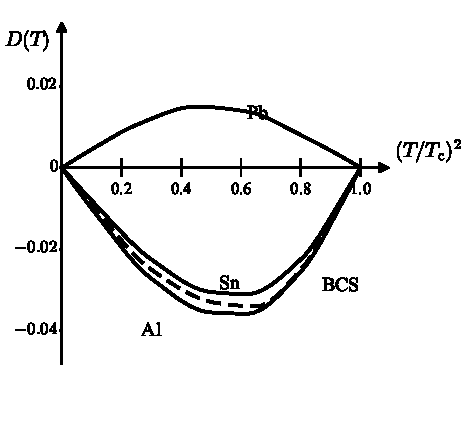
\includegraphics[width=6cm]{fig6-12.pdf}\\{\small 图 6.12\quad 实际临界磁场 $H_{\mathrm{c}}(T)/H_{\mathrm{c}}(0)$ 与经验曲线
$\left[1-(T/T_{\mathrm{c}})^{2}\right]$ 的差别}
\end{minipage}
\end{center}

这是由于Pb中的电子与声子耦合较强，基于二级微扰的BCS约化哈密顿量不再是良好的出发模型，而必须考虑耦合的高阶效应.对于强电声子耦合情形，必须从更为基本的电子与声子相互作用模型出发，运用格林函数技巧，考虑电子-声子-电子间互作用的推迟效应，屏蔽库仑作用以及热声子的激发等效应，才能给出与实验一致的结果，称为强耦合超导理论\textsuperscript{[5]}，而本章中所介绍的BCS理论则称为弱耦合的超导理论，它只适用于 $g(0)V\ll1$ 的情形.

\section{单粒子隧道效应}

利用超导与正常金属间的隧道效应，可直接测定能隙 $\Delta$，并验证BCS的态密度公式.本节着重讨论S-N系统的单粒子隧道效应\textsuperscript{[5]}.

设 $H_{1}$，$H_{2}$ 分别代表两块金属（1、2）的哈密顿量，它们的本征态为 $|\lambda_{1}\rangle$、$|\mu_{2}\rangle$，相应的能量本征值为 $\varepsilon_{\lambda}$ 和 $\varepsilon_{\mu}$
\begin{equation}
  H_{1}|\lambda_{1}\rangle=\varepsilon_{\lambda}|\lambda_{1}\rangle\text{，}
  \qquad H_{2}|\mu_{2}\rangle=\varepsilon_{\mu}|\mu_{2}\rangle
\end{equation}
电子在1、2两种金属间转移的隧道哈密顿量
\begin{equation}
  H_{\mathrm{T}}=\sum_{k,\,k'}\left(\mathscr{M}_{kk'}C^{(2)+}_{k'}C^{(1)}_{k}
  +\mathrm{h.c.}\right)
\end{equation}
系统的总哈密顿量为
\begin{equation}
  H=H_{1}+H_{2}+H_{\mathrm{T}}
\end{equation}
为简单起见，我们先讨论零温情况.根据含时微扰理论，当两块金属之间外加电压V时，它们的费密能相差为 $eV$，此时跃迁概率为
\begin{equation}
\begin{aligned}
  w_{12}=\frac{2\pi}{\hbar}\sum_{\lambda,\,\mu}
  \bigl|\langle\lambda_{1}|\langle\mu_{2}|
  \sum_{k,\,k'}\mathscr{M}_{kk'}C^{(2)+}_{k'}C^{(1)}_{k}
  |0_{2}\rangle|0_{1}\rangle\bigr|^{2}
  \times\delta\left(\varepsilon_{\lambda}+eV-\varepsilon_{\mu}\right)
\end{aligned}
\end{equation}
其中 $|0_{i}\rangle\ (i=1,2)$ 代表金属(1,2)的基态.这时单粒子隧穿电流
\begin{equation}
  I_{12}=ew_{12}
\end{equation}
由于 $V\ll E_{\mathrm{F}}$，参加跃迁的主要是费密面附近的电子，我们可以假定 $\mathscr{M}_{kk'}$ 近似为与k、$k'$ 无关的常数 $\mathscr{M}$，则式(6.6.4)可进一步简化
\begin{equation}
\begin{aligned}
  w_{12}&=\frac{2\pi}{\hbar}|\mathscr{M}|^{2}
  \int_{-\infty}^{\infty}\mathrm{d}\varepsilon
  \sum_{k,\,\lambda}|\langle\lambda_{1}|C^{(1)}_{k}|0_{1}\rangle|^{2}
  \delta(\varepsilon-\varepsilon_{\lambda})\times\\
  &\quad\sum_{k',\,\mu}|\langle\mu_{2}|C^{(2)+}_{k'}|0_{2}\rangle|^{2}
  \delta(\varepsilon+eV-\varepsilon_{\mu})\\
  &=\frac{2\pi}{\hbar}|\mathscr{M}|^{2}
  \int_{-\infty}^{\infty}\mathrm{d}\varepsilon\,
  N_{1}(\varepsilon)N_{2}(\varepsilon+eV)
\end{aligned}
\end{equation}
这里
\begin{equation}
  N_{1}(\varepsilon)\equiv\sum_{k,\,\lambda}
  |\langle\lambda_{1}|C^{(1)}_{k}|0_{1}\rangle|^{2}
  \delta\left(\varepsilon-\varepsilon_{\lambda}\right)
\end{equation}
\begin{equation}
  N_{2}(\varepsilon+eV)\equiv\sum_{k',\,\mu}
  |\langle\mu_{2}|C^{(2)+}_{k'}|0_{2}\rangle|^{2}
  \delta\left(\varepsilon+eV-\varepsilon_{\mu}\right)
\end{equation}
当1、2均为正常金属时
\begin{equation}
  \sum_{\lambda}|\langle\lambda_{1}|C^{(1)}_{k}|0_{1}\rangle|^{2}
  =\langle F|C^{(1)+}_{k}C^{(1)}_{k}|F\rangle
  =\left[1-\theta(\varepsilon_{k})\right]
\end{equation}
\begin{equation}
  \sum_{\mu}|\langle\mu_{2}|C^{(2)+}_{k'}|0_{2}\rangle|^{2}
  =\langle F|C^{(2)}_{k'}C^{(2)+}_{k'}|F\rangle
  =\theta(\varepsilon_{k'})
\end{equation}
其中 $\theta(\varepsilon)$ 为阶跃函数，即
\begin{equation}
  \theta(\varepsilon)=
  \begin{cases}1&(\varepsilon\geqslant0)\\0&(\varepsilon<0)\end{cases}
\end{equation}
由此求得 $T=0$ K时正常金属的
\begin{equation}
\begin{aligned}
  N_{1}(\varepsilon)&=\sum_{k}\left\{1-\theta(\varepsilon_{k})\right\}
  \delta\left(\varepsilon-\varepsilon_{k}\right)\\
  &=\int\mathrm{d}\varepsilon_{k}\,g_{1}(\varepsilon_{k})
  \left\{1-\theta(\varepsilon_{k})\right\}
  \delta\left(\varepsilon-\varepsilon_{k}\right)\\
  &=g_{1}(\varepsilon)\left\{1-\theta(\varepsilon)\right\}
\end{aligned}
\end{equation}
\begin{equation}
\begin{aligned}
  N_{2}(\varepsilon+eV)
  &=\sum_{k'}\theta\left(\varepsilon_{k'}\right)
  \delta\left(\varepsilon+eV-\varepsilon_{k'}\right)\\
  &=g_{2}(\varepsilon+eV)\,\theta(\varepsilon+eV)
\end{aligned}
\end{equation}
两块正常金属之间的隧穿电流
\begin{equation}
\begin{aligned}
  I_{\mathrm{NN}}&=\frac{2\pi e}{\hbar}|\mathscr{M}|^{2}
  \int_{-\infty}^{\infty}\mathrm{d}\varepsilon\,g_{1}(\varepsilon)\,
  g_{2}(\varepsilon+eV)\left\{1-\theta(\varepsilon)\right\}
  \theta\left(\varepsilon+eV\right)\\
  &=\frac{2\pi e}{\hbar}|\mathscr{M}|^{2}
  \int_{-\infty}^{\infty}\mathrm{d}\varepsilon\,g_{1}(\varepsilon)\,
  g_{2}(\varepsilon+eV)
  \left\{f(\varepsilon)\left[1-f(\varepsilon+eV)\right]\right\}_{T=0}
\end{aligned}
\end{equation}
用费密面上态密度 $g(0)$ 代替 $g(\varepsilon)$，可求得正常态的微分电导与V无关
\begin{equation}
\begin{aligned}
  G_{\mathrm{NN}}&=\left(\frac{\mathrm{d}I_{\mathrm{NN}}}{\mathrm{d}V}\right)_{T=0}
  \approx\frac{2\pi e^{2}}{\hbar}|\mathscr{M}|^{2}
  g_{1}(0)g_{2}(0)\int\mathrm{d}\varepsilon\,\delta\left(\varepsilon+eV\right)\\
  &=\frac{2\pi e^{2}}{\hbar}|\mathscr{M}|^{2}g_{1}(0)g_{2}(0)\equiv A
\end{aligned}
\end{equation}
\begin{equation}
  I_{\mathrm{NN}}(V)=AV
\end{equation}
$I-V$ 为直线关系，满足欧姆定律.

当金属1换为超导体时，应取
\begin{equation*}
  C^{(1)}_{k}=u_{k}\alpha_{k}+v_{k}\alpha^{+}_{-k}
\end{equation*}
此时
\begin{equation}
\begin{aligned}
  \sum_{\lambda}|\langle\lambda_{1}|C^{(1)}_{k}|0_{1}\rangle|^{2}
  &=\langle0_{1}|C^{(1)+}_{k}C^{(1)}_{k}|0_{1}\rangle\\
  &=v_{k}^{2}\ \langle0_{1}|\alpha_{-k}\alpha^{+}_{-k}|0_{1}\rangle=v_{k}^{2}
\end{aligned}
\end{equation}
准粒子能量为 $\xi_{k}=\sqrt{\varepsilon_{k}^{2}+\Delta^{2}}$，则式(6.6.7)写为
\begin{equation*}
\begin{aligned}
  N_{1\mathrm{S}}(\varepsilon)
  &=\sum_{k}v_{k}^{2}\delta\left(\varepsilon-\xi_{k}\right)
  =g_{1}(0)\int_{-\infty}^{\infty}\mathrm{d}\varepsilon_{k}\,
  v_{k}^{2}(\varepsilon_{k})\,\delta\left(\varepsilon-\xi_{k}\right)\\
  &=g_{1}(0)\int_{\Delta}^{\infty}\mathrm{d}\xi_{k}\,
  \left|\frac{\mathrm{d}\varepsilon_{k}}{\mathrm{d}\xi_{k}}\right|
  \left\{v_{k}^{2}(\varepsilon_{k})+v_{k}^{2}(-\varepsilon_{k})\right\}
  \delta\left(\varepsilon-\xi_{k}\right)
\end{aligned}
\end{equation*}
根据 $v_{k}^{2}=\frac{1}{2}\left(1-\frac{\varepsilon_{k}}{\xi_{k}}\right)$，可知 $v_{k}^{2}(-\varepsilon_{k})=u_{k}^{2}(\varepsilon_{k})$.因此，$u_{k}^{2}$ 与 $v_{k}^{2}$ 总是同时出现，上式中 $\{\cdots\}$ 因子简单地等于1.
\begin{equation}
  v_{k}^{2}(\varepsilon_{k})+v_{k}^{2}(-\varepsilon_{k})
  =v_{k}^{2}(\varepsilon_{k})+u_{k}^{2}(\varepsilon_{k})=1
\end{equation}
这时 $N_{1\mathrm{S}}(\varepsilon)$ 就是BCS的超导态密度，即
\begin{equation}
\begin{aligned}
  N_{1\mathrm{S}}(\varepsilon)
  &=g_{1}(0)\left|\frac{\mathrm{d}\varepsilon_{k}}{\mathrm{d}\xi_{k}}\right|_{\xi_{k}=\varepsilon}\\
  &=g_{1}(0)\,\mathrm{Re}\,\frac{|\varepsilon|}{\sqrt{\varepsilon^{2}-\Delta^{2}}}
  =g_{1\mathrm{S}}(\varepsilon)
\end{aligned}
\end{equation}
对于正常金属2，$N_{2}$ 仍由式(6.6.13)决定.这样S-N系统在 $T=0$ K时的单粒子隧穿电流为
\begin{equation}
\begin{aligned}
  I_{\mathrm{SN}}&=\frac{2\pi e}{\hbar}|\mathscr{M}|^{2}
  \int_{-\infty}^{\infty}\mathrm{d}\varepsilon\,
  N_{1\mathrm{S}}(\varepsilon)N_{2\mathrm{N}}(\varepsilon+eV)\\
  &=\frac{2\pi e}{\hbar}|\mathscr{M}|^{2}g_{2}(0)
  \int_{-\infty}^{\infty}\mathrm{d}\varepsilon\,
  g_{1\mathrm{S}}(\varepsilon)\,\theta(\varepsilon+eV)
\end{aligned}
\end{equation}
其微分电导为
\begin{equation}
\begin{aligned}
  G_{\mathrm{SN}}&=\left(\frac{\mathrm{d}I_{\mathrm{SN}}}{\mathrm{d}V}\right)_{T=0}
  =\frac{2\pi e^{2}}{\hbar}|\mathscr{M}|^{2}g_{2}(0)
  \int_{-\infty}^{\infty}\mathrm{d}\varepsilon\,
  g_{1\mathrm{S}}(\varepsilon)\,\delta\left(\varepsilon+eV\right)\\
  &=\frac{2\pi e^{2}}{\hbar}|\mathscr{M}|^{2}g_{1}(0)g_{2}(0)
  \int\mathrm{d}\varepsilon\,\frac{g_{1\mathrm{S}}(\varepsilon)}{g_{1}(0)}
  \,\delta(\varepsilon+eV)\\
  &=A\,\mathrm{Re}\,\frac{|eV|}{\sqrt{(eV)^{2}-\Delta^{2}}}
\end{aligned}
\end{equation}
其中A代表 $G_{\mathrm{NN}}$，由式(6.6.15)决定，注意超导态微分电导与正常态微分电导之比是
\begin{equation}
  \frac{G_{\mathrm{SN}}}{G_{\mathrm{NN}}}
  =\mathrm{Re}\,\frac{|eV|}{\sqrt{(eV)^{2}-\Delta^{2}}}
  =g_{1\mathrm{S}}(\varepsilon)\qquad(\varepsilon=eV)
\end{equation}
测定这个比值将给出超导体中的准粒子态密度.根据式(6.6.21)，还可以导出零温隧穿电流为
\begin{equation}
  I_{\mathrm{SN}}(V)=A\,\mathrm{Re}\sqrt{(eV)^{2}-\Delta^{2}}
\end{equation}
现在讨论有限温度情况.对于 $I_{\mathrm{NN}}$，可根据式(6.6.14)再计入反向电子跃迁项
\begin{equation*}
  \frac{2\pi e}{\hbar}|\mathscr{M}|^{2}\int_{-\infty}^{\infty}
  \mathrm{d}\varepsilon\,g_{1}(\varepsilon)g_{2}(\varepsilon+eV)
  \left[1-f(\varepsilon)\right]f(\varepsilon+eV)
\end{equation*}
求得 $T\neq0$ K时的
\begin{equation}
  I_{\mathrm{NN}}=\frac{2\pi e}{\hbar}|\mathscr{M}|^{2}
  \int_{-\infty}^{\infty}\mathrm{d}\varepsilon\,g_{1}(\varepsilon)\,
  g_{2}(\varepsilon+eV)
  \left[f(\varepsilon)-f(\varepsilon+eV)\right]
\end{equation}
在低温和小电压情况下 $\left(1\ll\beta E_{\mathrm{F}},\,eV\ll E_{\mathrm{F}}\right)$ 这个积分容易算出，其结果近似为式(6.6.16)，与零温情况没有太大差别.

对于S-N系统，式(6.6.17)应换为热平均 $\langle C^{(1)+}_{k}C^{(1)}_{k}\rangle_{T}$，其中 $\langle\alpha_{-k}\alpha^{+}_{-k}\rangle_{T}=1-f(\xi_{k})$.详细讨论的结果与 $I_{\mathrm{NN}}$ 相仿，只需将式(6.6.24)中 $g_{1}(\varepsilon)$ 换成 $g_{1\mathrm{S}}(\varepsilon)$，即是
\begin{equation}
  I_{\mathrm{SN}}=\frac{2\pi e}{\hbar}|\mathscr{M}|^{2}
  \int_{-\infty}^{\infty}\mathrm{d}\varepsilon\,
  g_{1\mathrm{S}}(\varepsilon)\,g_{2\mathrm{N}}(\varepsilon+eV)
  \left[f(\varepsilon)-f(\varepsilon+eV)\right]
\end{equation}
利用式(6.6.19)求得 $T\neq0$ K时的微分电导为
\begin{equation}
\begin{aligned}
  G_{\mathrm{SN}}=\frac{\mathrm{d}I_{\mathrm{SN}}}{\mathrm{d}V}
  =\frac{2\pi e^{2}}{\hbar}|\mathscr{M}|^{2}g_{1}(0)g_{2}(0)
  &\left(\int_{\Delta}^{\infty}\frac{|\varepsilon|}{\sqrt{\varepsilon^{2}-\Delta^{2}}}\,
  \frac{\beta\exp\left[\beta(\varepsilon+eV)\right]}
  {\left\{1+\exp\left[\beta(\varepsilon+eV)\right]\right\}^{2}}\mathrm{d}\varepsilon\right.\\
  \left.+\int_{-\infty}^{-\Delta}\frac{|\varepsilon|}{\sqrt{\varepsilon^{2}-\Delta^{2}}}\,
  \frac{\beta\exp\left[\beta(\varepsilon+eV)\right]}
  {\left\{1+\exp\left[\beta(\varepsilon+eV)\right]\right\}^{2}}\mathrm{d}\varepsilon\right)
\end{aligned}
\end{equation}
式(6.6.26)可按贝塞尔函数展开计算.图6.13中实线为 $T=0$ K的情况，它表明在超导体的准粒子态密度中存在能隙 $\Delta$，虚线为 $T>0$ K时的 $G_{\mathrm{SN}}/G_{\mathrm{NN}}$ 曲线，它与 $T=0$ K情况的主要差别是在 $eV<\Delta$ 区域内仍存在隧穿电流.当 $k_{\mathrm{B}}T\ll\Delta$ 和 $V\to0$ 时，式(6.6.26)容易计算，其近似结果为
\begin{equation*}
\begin{aligned}
  \lim_{\substack{T\to0\\ V\to0}}
  \left[\frac{\mathrm{d}I_{\mathrm{SN}}}{\mathrm{d}V}\right]
  &\approx 2A\int_{-\infty}^{-\Delta}\mathrm{d}\varepsilon\,
  \frac{|\varepsilon|}{\sqrt{\varepsilon^{2}-\Delta^{2}}}\,
  \beta\exp\left(\beta\varepsilon\right)\\
  &\approx 2A\int_{\Delta}^{\infty}\mathrm{d}\varepsilon\,
  \frac{|\varepsilon|}{\sqrt{\varepsilon^{2}-\Delta^{2}}}\,
  \beta\exp\left(-\beta\varepsilon\right)\\
  &=2A\beta\int_{0}^{\infty}\mathrm{d}x\,
  \mathrm{e}^{-\beta\sqrt{x^{2}+\Delta^{2}}}\\
  &\approx 2A\beta\int_{0}^{\infty}\mathrm{d}x\,
  \mathrm{e}^{-\beta\Delta(0)\left[1+\frac{x^{2}}{2\Delta^{2}(0)}\right]}
\end{aligned}
\end{equation*}
\begin{equation}
  =A\left[\frac{2\pi\Delta(0)}{k_{\mathrm{B}}T}\right]^{1/2}
  \mathrm{e}^{-\Delta(0)/k_{\mathrm{B}}T}
\end{equation}

\begin{center}
\begin{minipage}{6.5cm}
\centering
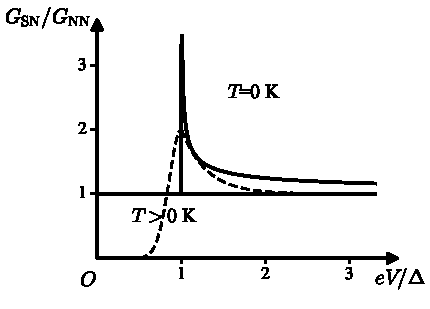
\includegraphics[width=6.5cm]{fig6-13.pdf}\\{\small 图 6.13\quad S-N系统的微分电导}
\end{minipage}
\end{center}

相应的，在低温和小电压情况下隧穿电流之比为
\begin{equation}
  \lim_{\substack{T\to0\\ V\to0}}\frac{I_{\mathrm{SN}}}{I_{\mathrm{NN}}}
  =\left[\frac{2\pi\Delta(0)}{k_{\mathrm{B}}T}\right]^{1/2}
  \mathrm{e}^{-\Delta(0)/k_{\mathrm{B}}T}
\end{equation}
如图6.14中虚线所示，与贾埃弗（Giaever）\textsuperscript{[6]}的实验结果一致（参考图6.3），直接证实了超导体中单个准粒子激发至少需要 $\Delta$ 能量，即存在能隙.

\begin{center}
\begin{minipage}{6cm}
\centering
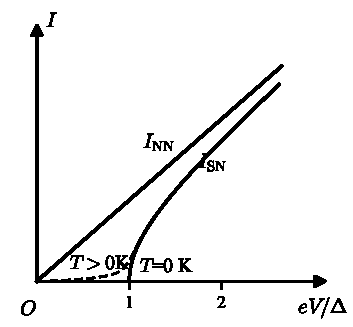
\includegraphics[width=6cm]{fig6-14.pdf}\\{\small 图 6.14\quad $I$-$V$ 曲线}
\end{minipage}
\end{center}

\section{伦敦-皮帕的唯象理论}

超导体的主要特征为：

（i）$T<T_{\mathrm{c}}$ 时直流电阻消失，存在着无阻的超电流，这是超导体的理想导电性.

（ii）迈斯纳效应，弱磁场不能透入大块超导样品内部，表现出完全逆磁性.

在这两个主要特征的基础上，伦敦建立了描述超导体电磁性质的唯象理论，皮帕又进一步将它推广到包含了磁场的非定域情形.

\subsection*{1. 伦敦方程}

正常金属的电阻效应由欧姆定律 $\boldsymbol{j}=\sigma\boldsymbol{E}$ 描述.为了描述超导体的理想导电性和完全逆磁性，应当有新的关系式.伦敦假定超电流 $\boldsymbol{j}_{\mathrm{s}}(\boldsymbol{r})$ 与电磁场的矢量势 $\boldsymbol{A}(\boldsymbol{r})$ 成正比
\begin{equation}
  \boldsymbol{j}_{\mathrm{s}}=-\frac{1}{c\Lambda}\boldsymbol{A}
  \qquad\left(\Lambda=\frac{m}{n_{\mathrm{s}}e^{2}}\right)
\end{equation}
其比例常量为负数.下面将看到，正是这个负号说明超电流的屏蔽作用，从而保证了完全逆磁性.其中 $n_{\mathrm{s}}$ 代表超导电子浓度，当 $T=0$ K时 $n_{\mathrm{s}}=n$，n即传导电子密度.$\boldsymbol{A}$ 满足横场条件 $\nabla\cdot\boldsymbol{A}=0$.式(6.7.1)被称为伦敦方程，它与麦克斯韦（Maxwell）方程组合可说明超导体的电动力学性质.我们只说明式(6.7.1)包含了超导体的两个主要特征.

（i）理想导电性：式(6.7.1)两边对时间取导数，得
\begin{equation}
  \frac{\partial}{\partial t}\left(\Lambda\boldsymbol{j}_{\mathrm{s}}\right)
  =-\frac{1}{c}\frac{\partial\boldsymbol{A}}{\partial t}=\boldsymbol{E}
\end{equation}
式(6.7.2)就是超导电子的无阻运动方程
$\dfrac{\partial}{\partial t}\left(m\boldsymbol{v}_{\mathrm{s}}\right)=e\boldsymbol{E}$
和 $j_{\mathrm{s}}=n_{\mathrm{s}}e\boldsymbol{v}_{\mathrm{s}}$ 的组合.因此，它代表超导体的理想导电性.式(6.7.2)说明当电场 $\boldsymbol{E}=0$ 时，也存在 $\boldsymbol{j}_{\mathrm{s}}=$ 常数的超导持续电流.

（ii）完全逆磁性：对式(6.7.1)两边取旋度，得到方程
\begin{equation}
  \boldsymbol{B}=-c\Lambda\,\nabla\times\boldsymbol{j}_{\mathrm{s}}
\end{equation}
再利用麦克斯韦方程 $\nabla\times\boldsymbol{B}=\dfrac{4\pi}{c}\boldsymbol{j}_{\mathrm{s}}$ 和 $\nabla\cdot\boldsymbol{B}=0$，求得
\begin{equation}
  \nabla^{2}\boldsymbol{B}=\frac{1}{\lambda_{\mathrm{L}}^{2}}\boldsymbol{B}
  \qquad\left(\lambda_{\mathrm{L}}^{2}=\frac{mc^{2}}{4\pi n_{\mathrm{s}}e^{2}}\right)
\end{equation}
对于 $z>0$ 的半无限超导样品，当外磁场平行于 $z=0$ 平面时，式(6.7.3)简化为
\begin{equation}
  \frac{\mathrm{d}^{2}\boldsymbol{B}}{\mathrm{d}z^{2}}
  =\frac{\boldsymbol{B}}{\lambda_{\mathrm{L}}^{2}}
\end{equation}
其指数衰减解为
\begin{equation}
  \boldsymbol{B}(z)=\boldsymbol{B}(0)\exp\left(-z/\lambda_{\mathrm{L}}\right)
\end{equation}
上式说明，只在样品表面内约为 $\lambda_{\mathrm{L}}$ 厚度的薄层内存在磁场，深入到样品内部时 $\boldsymbol{B}$ 已下降到零.对于超电流 $j_{\mathrm{s}}$ 利用式(6.7.3)和麦克斯韦方程同样可求得
\begin{equation}
  \nabla^{2}\boldsymbol{j}_{\mathrm{s}}=\frac{1}{\lambda_{\mathrm{L}}^{2}}\boldsymbol{j}_{\mathrm{s}}
\end{equation}
因此，在恒定磁场中超导电流也分布在表面内 $\lambda_{\mathrm{L}}$ 厚度中，相应的 $\boldsymbol{A}$ 也在 $\lambda_{\mathrm{L}}$ 尺度上降为零.不难验证，$j_{\mathrm{s}}$ 起着屏蔽样品内部磁场的作用.例如，在上述半无限样品中，若设外磁场沿正x轴方向，则根据伦敦方程(6.7.1)，$j_{\mathrm{s}}$ 沿y轴负方向.通过 $\nabla\times\boldsymbol{B}=\dfrac{4\pi}{c}\boldsymbol{j}_{\mathrm{s}}$，可判断超导流 $j_{\mathrm{s}}$ 的磁场取向，它恰好沿x轴负方向，起着屏蔽外磁场的作用，使大块样品内部的磁感应强度 $\boldsymbol{B}=0$，此即迈斯纳效应.所以，伦敦方程也反映了超导体的完全逆磁性. $\lambda_{\mathrm{L}}$ 代表磁场透入超导样品的深度，称为穿透深度，它是超导体的一个重要特征参量.伦敦方程可以用 $\lambda_{\mathrm{L}}$ 表示为
\begin{equation}
  \boldsymbol{j}_{\mathrm{s}}(\boldsymbol{r})
  =-\frac{c}{4\pi}\frac{1}{\lambda_{\mathrm{L}}^{2}}\boldsymbol{A}(\boldsymbol{r})
\end{equation}
式(6.7.8)说明当穿透深度增大时，超电流减小.当 $T=0$ 时
\begin{equation}
  \lambda_{\mathrm{L}}(0)=\left(\frac{mc^{2}}{4\pi ne^{2}}\right)^{\frac{1}{2}}
\end{equation}
对于纯金属超导样品，$\lambda_{\mathrm{L}}(0)$ 约为 $10^{-6}\sim10^{-5}$ cm量级.但是，实验测定值往往比 $\lambda_{\mathrm{L}}(0)$ 大好几倍.这是因为伦敦方程忽略了超导体的另一个重要参量——相干长度 $\xi_{0}$ 的影响.

\subsection*{2. 皮帕公式}

伦敦方程(6.7.1)假定超电流密度 $\boldsymbol{j}_{\mathrm{s}}(\boldsymbol{r})$ 正比于同一点的矢量势 $\boldsymbol{A}(\boldsymbol{r})$，这是一个定域的关系式.但是，超导体中由于在相干长度 $\xi_{0}=\dfrac{\hbar v_{\mathrm{F}}}{\pi\Delta(0)}$ 范围内存在着电子运动的关联，因此作用于某一点的扰动势必将会影响 $\xi_{0}$ 空间尺度内超导电子的运动速度和电流密度.反过来，在空间某一点的超电流密度也必定会受到其邻近 $\xi_{0}$ 尺度内扰动势的影响.这样，$\boldsymbol{j}_{\mathrm{s}}(\boldsymbol{r})$ 不仅决定于同一点的 $\boldsymbol{A}(\boldsymbol{r})$，还应当包括 $|\boldsymbol{r}-\boldsymbol{r}'|<\xi_{0}$ 范围内各点 $\boldsymbol{r}'$ 的矢量势 $\boldsymbol{A}(\boldsymbol{r}')$ 的贡献.为此，皮帕假定 $j_{\mathrm{s}}$ 与A的非定域关系为
\begin{equation}
  \boldsymbol{j}_{\mathrm{s}}(\boldsymbol{r})
  =-\frac{3}{4\pi\xi_{0}\Lambda c}
  \int\frac{\boldsymbol{R}\left[\boldsymbol{R}\cdot\boldsymbol{A}(\boldsymbol{r}')\right]}
  {R^{4}}\,\mathrm{e}^{-R/\xi_{0}}\mathrm{d}\boldsymbol{r}'
  \qquad\left(\boldsymbol{R}=\boldsymbol{r}-\boldsymbol{r}'\right)
\end{equation}
当A在 $\xi_{0}$ 距离上变化缓慢时，A可以从积分号中提出，从而求得定域关系：
\begin{equation}
\begin{aligned}
  \left[j_{\mathrm{s}}(\boldsymbol{r})\right]_{\mu}
  &\approx-\frac{1}{\xi_{0}\Lambda c}\sum_{\nu}A_{\nu}(\boldsymbol{r})
  \frac{3}{4\pi}\int\mathrm{d}^{3}R\,R_{\mu}R_{\nu}\,
  \frac{\mathrm{e}^{-R/\xi_{0}}}{R^{4}}\\
  &=\frac{1}{\Lambda c}\sum_{\nu}A_{\nu}(\boldsymbol{r})\,\delta_{\mu\nu}
  \left[\frac{1}{\xi_{0}}\int_{0}^{R}\mathrm{d}R\,\mathrm{e}^{-R/\xi_{0}}\right]\\
  &=-\frac{1}{\Lambda c}A_{\mu}(\boldsymbol{r})
\end{aligned}
\end{equation}
式(6.7.11)的矢量表示式即伦敦方程.根据“1”中讨论A在穿透深度 $\lambda_{\mathrm{L}}$ 范围内指数衰减为零.因此，伦敦方程只适用于 $\lambda_{\mathrm{L}}\gg\xi_{0}$ 情况，这时在 $\xi_{0}$ 尺度上j与A的变化都很缓慢.但是纯金属的 $\lambda_{\mathrm{L}}\ll\xi_{0}$，显然纯金属中A在 $\xi_{0}$ 尺度上变化很急剧，这时伦敦方程不适用，必须应用皮帕公式(6.7.10)，所算出的超电流 $j_{\mathrm{s}}$ 必然比按照伦敦方程计算的小.由于超电流减小，意味着穿透深度的增大，因此按式(6.7.10)算出的穿透深度 $\lambda_{\text{理}}$ 将比 $\lambda_{\mathrm{L}}(0)$ 大.精确计算的结果列于表6.2中，它与实验测量值基本相符.因此伦敦穿透深度 $\lambda_{\mathrm{L}}$ 与实验值有分歧的原因是忽略了磁场的非定域效应.不仅如此，将皮帕公式推广用于含杂质超导体，也圆满地解释了实验事实\textsuperscript{[7]}.总之，皮帕公式适用于更普遍的情况.在下一节中我们将看到从BCS理论导出的 $j_{\mathrm{s}}$ 和A关系与皮帕公式相近，可认为是伦敦-皮帕唯象理论的微观证明.

\begin{center}
\begin{minipage}{10.5cm}\centering\small
表 6.2\\[0.5em]
\begin{tabular}{lcccc}
\hline
纯金属 & $\lambda_{\mathrm{L}}$/nm & $\xi_{0}$/nm & $\lambda_{\text{理}}$/nm & $\lambda_{\text{实}}$/nm\\
\hline
Al & $157\times10^{-1}$ & $16\,000\times10^{-1}$ & $530\times10^{-1}$ & $(490\sim515)\times10^{-1}$\\
Sn & $355\times10^{-1}$ & $2\,300\times10^{-1}$ & $560\times10^{-1}$ & $510\times10^{-1}$\\
\hline
\end{tabular}
\end{minipage}
\end{center}

为了将在§8中讨论方便起见，在这里先给出伦敦-皮帕公式的傅里叶变换表示式.利用下列变换式：
\begin{equation}
  \left.
  \begin{aligned}
    \boldsymbol{j}(\boldsymbol{q})
    &=\int\mathrm{d}^{3}r\,\mathrm{e}^{-\mathrm{i}\boldsymbol{q}\cdot\boldsymbol{r}}
    \boldsymbol{j}(\boldsymbol{r})\\
    \boldsymbol{A}(\boldsymbol{q})
    &=\int\mathrm{d}^{3}r\,\mathrm{e}^{-\mathrm{i}\boldsymbol{q}\cdot\boldsymbol{r}}
    \boldsymbol{A}(\boldsymbol{r})
  \end{aligned}\right\}
\end{equation}
可立刻求得零温伦敦方程式(6.7.8)的傅里叶变换公式
\begin{equation}
  \boldsymbol{j}(\boldsymbol{q})
  =-\frac{c}{4\pi}K_{\mathrm{L}}(q)\boldsymbol{A}(\boldsymbol{q})
\end{equation}
其中
\begin{equation}
  K_{\mathrm{L}}(q)=K_{\mathrm{L}}(0)=\lambda_{\mathrm{L}}^{-2}(0)
\end{equation}
对于皮帕公式(6.7.10)
\begin{equation}
  \boldsymbol{j}(\boldsymbol{q})=-\frac{c}{4\pi}\frac{1}{\lambda_{\mathrm{L}}^{2}(0)}
  \frac{3}{4\pi\xi_{0}}\int\mathrm{d}^{3}R\,
  \frac{\boldsymbol{R}\left[\boldsymbol{R}\cdot\boldsymbol{A}(\boldsymbol{q})\right]}{R^{4}}\,
  \mathrm{e}^{-R/\xi_{0}}\mathrm{e}^{-\mathrm{i}\boldsymbol{q}\cdot\boldsymbol{R}}
\end{equation}
利用横场条件 $\boldsymbol{q}\cdot\boldsymbol{A}(\boldsymbol{q})=0$（即 $\nabla\cdot\boldsymbol{A}=0$），不难求出
\begin{equation}
  \boldsymbol{j}(\boldsymbol{q})
  =-\frac{c}{4\pi}K(q)\boldsymbol{A}(\boldsymbol{q})
\end{equation}
\begin{equation}
  K(q)=\frac{1}{\lambda_{\mathrm{L}}^{2}(0)\xi_{0}}
  \int_{0}^{\infty}\mathrm{d}R\,\mathrm{e}^{-R/\xi_{0}}
  \left\{\frac{3}{qR}\mathrm{j}_{1}(qR)\right\}
\end{equation}
其中 $\mathrm{j}_{1}$ 为球贝塞尔函数：
\begin{equation}
  \mathrm{j}_{1}(x)=\frac{\sin x}{x^{2}}-\frac{\cos x}{x}
\end{equation}
皮帕的 $K(q)$ 如图6.15所示.在两个极限情况下的 $K(q)$ 分别为

\begin{center}
\begin{minipage}{5.5cm}
\centering
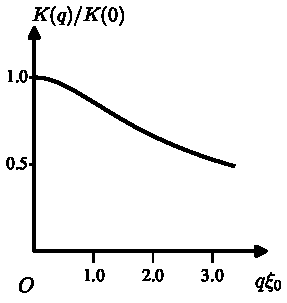
\includegraphics[width=5.5cm]{fig6-15.pdf}\\{\small 图 6.15\quad 皮帕的 $K(q)$}
\end{minipage}
\end{center}

（i）$q\xi_{0}\ll1$，积分式(6.7.17)主要贡献在 $qR=0$ 处，考虑到 $\left\{\dfrac{3}{qR}\mathrm{j}_{1}(qR)\right\}$ 相对于指数因子为缓变函数，可取
\begin{equation*}
  \lim_{qR\to0}\left\{\frac{3}{qR}\mathrm{j}_{1}(qR)\right\}=1
\end{equation*}
则
\begin{equation}
\begin{aligned}
  K(q)\approx K(0)&=\frac{1}{\lambda_{\mathrm{L}}^{2}(0)}
  \left\{\frac{1}{\xi_{0}}\int_{0}^{\infty}\mathrm{d}R\,\mathrm{e}^{-R/\xi_{0}}\right\}
  =\frac{1}{\lambda_{\mathrm{L}}^{2}(0)}\\
  &=K_{\mathrm{L}}(0)\qquad(q\xi_{0}\ll1)
\end{aligned}
\end{equation}
（ii）$q\xi_{0}\gg1$：将式(6.7.17)中指数因子近似用1代替，求出
\begin{equation}
\begin{aligned}
  K(q)&\approx\frac{1}{\lambda_{\mathrm{L}}^{2}(0)}
  \left(\frac{1}{q\xi_{0}}\right)\int_{0}^{\infty}\frac{3}{x}\mathrm{j}_{1}(x)\,\mathrm{d}x\\
  &=K(0)\frac{3\pi}{4q\xi_{0}}\qquad(q\xi_{0}\gg1)
\end{aligned}
\end{equation}

\section{迈斯纳效应}

我们将从BCS理论出发研究超导体在弱磁场中的行为，它属于超导体与电磁场互作用的静态 $\left(\omega=0\right)$ 极限情况.根据§7中的讨论可知，如果在 $q\to0$ 时求得的公式
$\boldsymbol{j}(\boldsymbol{q})=-\dfrac{c}{4\pi}\boldsymbol{K}(q)\boldsymbol{A}(\boldsymbol{q})$
中 $K(0)>0$，就表示有迈斯纳效应，若 $K(0)=0$，则无迈斯纳效应.此外，在本节中我们还要从微观角度证明超电流与矢量势的非定域关系.为简单起见仅讨论 $T=0$ K情况.

\subsection*{1. 互作用哈密顿量H}

互作用项 $H_{1}$ 由外场中动能的增量决定，在弱磁场作用下，准至A的线性项时得
\begin{equation}
  \frac{1}{2m}\left(\hat{\boldsymbol{p}}-\frac{e}{c}\boldsymbol{A}\right)^{2}
  -\frac{1}{2m}\hat{\boldsymbol{p}}^{2}
  \approx\frac{\mathrm{i}e\hbar}{2mc}
  \left(\boldsymbol{A}\cdot\nabla+\nabla\cdot\boldsymbol{A}\right)
\end{equation}
$H_{1}$ 的二次量子化表示式为
\begin{equation}
  H_{1}=\frac{\mathrm{i}e\hbar}{2mc}\int
  \Psi^{+}\left(\boldsymbol{A}\cdot\nabla+\nabla\cdot\boldsymbol{A}\right)
  \Psi\,\mathrm{d}\boldsymbol{r}
\end{equation}
按傅里叶级数展开矢量势，得
\begin{equation}
  \boldsymbol{A}(\boldsymbol{r})=\sum_{\boldsymbol{q}}
  \boldsymbol{A}(\boldsymbol{q})\,\mathrm{e}^{\mathrm{i}\boldsymbol{q}\cdot\boldsymbol{r}}
\end{equation}
将 $\Psi$ 按平面波展开，设样品取单位体积时
\begin{equation}
  \Psi(\boldsymbol{r})=\sum_{k,\,\sigma}C_{k\sigma}\,
  \mathrm{e}^{\mathrm{i}\boldsymbol{k}\cdot\boldsymbol{r}}\chi_{\sigma}
\end{equation}
当 $\sigma=\pm1$ 时，$\chi_{\sigma}$ 分别为 $\binom{1}{0}$ 和 $\binom{0}{1}$，$\chi_{\sigma}$ 满足关系
\begin{equation}
  \chi^{+}_{\sigma'}\chi_{\sigma}=\delta_{\sigma'\sigma}
\end{equation}
因此
\begin{equation}
\begin{aligned}
  H_{1}&=-\frac{e\hbar}{2mc}\sum_{k,\,k',\,q,\,\sigma}
  C^{+}_{k'\sigma}C_{k\sigma}\left(2\boldsymbol{k}+\boldsymbol{q}\right)
  \cdot\boldsymbol{A}(\boldsymbol{q})
  \int\mathrm{e}^{\mathrm{i}\left(\boldsymbol{k}+\boldsymbol{q}-\boldsymbol{k}'\right)
  \cdot\boldsymbol{r}}\mathrm{d}\boldsymbol{r}\\
  &=-\frac{e\hbar}{2mc}\sum_{k,\,q,\,\sigma}
  \left(2\boldsymbol{k}+\boldsymbol{q}\right)\cdot\boldsymbol{A}(\boldsymbol{q})\,
  C^{+}_{k+q,\,\sigma}C_{k\sigma}
\end{aligned}
\end{equation}
磁场矢量势采用横场规范 $\boldsymbol{q}\cdot\boldsymbol{A}(\boldsymbol{q})=0$，并根据§2中约定记 $(\boldsymbol{k},\uparrow)$ 为k，记 $(-\boldsymbol{k},\downarrow)$ 为$-k$，可将式(6.8.6)改写成
\begin{equation}
  H_{1}=-\frac{e\hbar}{mc}\sum_{k,\,q}
  \left[\boldsymbol{k}\cdot\boldsymbol{A}(\boldsymbol{q})\right]
  \left(C^{+}_{k+q}C_{k}-C^{+}_{-k}C_{-k-q}\right)
\end{equation}
再利用式(6.4.15)，将 $H_{1}$ 用超导元激发算符 $\alpha$、$\alpha^{+}$ 表示：
\begin{equation}
\begin{aligned}
  H_{1}=-\frac{e\hbar}{mc}\sum_{k,\,q}
  \left[\boldsymbol{k}\cdot\boldsymbol{A}(\boldsymbol{q})\right]
  &\left[\left(u_{k+q}v_{k}-u_{k}v_{k+q}\right)
  \left(\alpha^{+}_{k+q}\alpha^{+}_{-k}
  +\alpha_{k}\alpha_{-k-q}\right)\right.\\
  \left.+\left(u_{k+q}u_{k}+v_{k+q}v_{k}\right)
  \left(\alpha^{+}_{k+q}\alpha_{k}
  -\alpha^{+}_{-k}\alpha_{-k-q}\right)\right]
\end{aligned}
\end{equation}

\subsection*{2. 电流密度算符}

根据量子力学，电磁场中电流密度算符可由连续性方程导出，其二次量子化表示为
\begin{equation}
\begin{aligned}
  \hat{\boldsymbol{j}}(\boldsymbol{r})
  &=\frac{e\hbar}{2m\mathrm{i}}\left[\Psi^{+}\left(\nabla\Psi\right)
  -\left(\nabla\Psi^{+}\right)\Psi\right]
  -\frac{e^{2}}{mc}\Psi^{+}\boldsymbol{A}\Psi\\
  &\equiv\hat{\boldsymbol{j}}_{1}(\boldsymbol{r})+\hat{\boldsymbol{j}}_{2}(\boldsymbol{r})
\end{aligned}
\end{equation}
其中
\begin{equation}
\begin{aligned}
  \hat{\boldsymbol{j}}_{1}(\boldsymbol{r})
  &\equiv\frac{e\hbar}{2m\mathrm{i}}\left[\Psi^{+}\left(\nabla\Psi\right)
  -\left(\nabla\Psi^{+}\right)\Psi\right]\\
  &=\frac{e\hbar}{2m}\sum_{k,\,q}\left(2\boldsymbol{k}+\boldsymbol{q}\right)
  \mathrm{e}^{-\mathrm{i}\boldsymbol{q}\cdot\boldsymbol{r}}
  \left(C^{+}_{k+q}C_{k}-C^{+}_{-k}C_{-k-q}\right)
\end{aligned}
\end{equation}
\begin{equation}
\begin{aligned}
  \hat{\boldsymbol{j}}_{2}(\boldsymbol{r})
  &\equiv-\frac{e^{2}}{mc}\Psi^{+}\boldsymbol{A}\Psi\\
  &=-\frac{e^{2}}{mc}\boldsymbol{A}(\boldsymbol{r})\sum_{k,\,q}
  \mathrm{e}^{-\mathrm{i}\boldsymbol{q}\cdot\boldsymbol{r}}
  \left(C^{+}_{k+q}C_{k}+C^{+}_{-k}C_{-k-q}\right)
\end{aligned}
\end{equation}
这里已采用了与式(6.8.7)相同的约定符号.

式(6.8.11)中的负号说明它代表逆磁电流部分.在弱磁场作用下，只需计算到A的一阶，这时可用零场时的超导基态 $|0\rangle_{0}$ 对 $\hat{j}_{2}$ 求平均，得到 $T=0$ K时的电流响应
\begin{equation*}
\begin{aligned}
  \boldsymbol{j}_{2}(\boldsymbol{r})
  &\equiv\langle\hat{\boldsymbol{j}}_{2}(\boldsymbol{r})\rangle_{0}\\
  &=-\frac{e^{2}}{mc}\boldsymbol{A}(\boldsymbol{r})\sum_{k,\,q}
  \mathrm{e}^{-\mathrm{i}\boldsymbol{q}\cdot\boldsymbol{r}}
  \,_{0}\langle0|\left(C^{+}_{k+q}C_{k}+C^{+}_{-k}C_{-k-q}\right)|0\rangle_{0}
\end{aligned}
\end{equation*}
上式中，只有 $q=0$ 项有贡献，并且 $_{0}\langle0|C^{+}_{k}C_{k}|0\rangle_{0}=v_{k}^{2}
=\,_{0}\langle0|C^{+}_{-k}C_{-k}|0\rangle_{0}$，这时
\begin{equation*}
  \boldsymbol{j}_{2}(\boldsymbol{r})=-\frac{e^{2}}{mc}\boldsymbol{A}(\boldsymbol{r})
  \sum_{k}2v_{k}^{2}
  =-\frac{e^{2}}{mc}\boldsymbol{A}(\boldsymbol{r})
  \sum_{k}\left(1-\frac{\varepsilon_{k}}{\xi_{k}}\right)
\end{equation*}
上式右边第二项是 $\varepsilon_{k}$ 的奇函数，它对 $j_{2}$ 无贡献.另外，在样品取单位体积时，应有 $\sum_{k}1=n$，代表传导电子密度.因此
\begin{equation}
  \boldsymbol{j}_{2}(\boldsymbol{r})=\frac{ne^{2}}{mc}\boldsymbol{A}(\boldsymbol{r})
  =-\frac{c}{4\pi}\lambda_{\mathrm{L}}^{-2}(0)\boldsymbol{A}(\boldsymbol{r})
\end{equation}
即伦敦方程(6.7.8).读者不难自行验证，式(6.8.12)的结果对于正常态和超导态是一样的.因此，证明迈斯纳效应的关键在于对 $\boldsymbol{j}_{1}(\boldsymbol{r})$ 的计算.$\hat{j}_{1}$ 的元激发算符表示式为
\begin{equation}
\begin{aligned}
  \hat{\boldsymbol{j}}_{1}(\boldsymbol{r})
  =\frac{e\hbar}{2m}\sum_{k,\,q}&\left(2\boldsymbol{k}+\boldsymbol{q}\right)
  \mathrm{e}^{-\mathrm{i}\boldsymbol{q}\cdot\boldsymbol{r}}
  \left\{\left(u_{k+q}v_{k}-u_{k}v_{k+q}\right)
  \left(\alpha^{+}_{k+q}\alpha^{+}_{-k}
  +\alpha_{k}\alpha_{-k-q}\right)\right.\\
  &+\left.\left(u_{k+q}u_{k}+v_{k+q}v_{k}\right)
  \left(\alpha^{+}_{k+q}\alpha_{k}
  -\alpha^{+}_{-k}\alpha_{-k-q}\right)\right\}
\end{aligned}
\end{equation}

\subsection*{3. 弱磁场中的电流响应}

计算 $\hat{j}_{1}$ 时，应当考虑A对超导态的影响，利用微扰论，准至A一阶的状态为
\begin{equation}
  |0\rangle_{1}=|0\rangle_{0}
  +{\sum_{l}}'\,|l\rangle_{0}\,
  \frac{_{0}\langle l|H_{1}|0\rangle_{0}}{E_{0}-E_{l}}
\end{equation}
而
\begin{equation}
\begin{aligned}
  \boldsymbol{j}_{1}(\boldsymbol{r})
  ={}_{0}\langle0|\hat{j}_{1}|0\rangle_{0}
  +{\sum_{l}}'\biggl\{&\frac{_{0}\langle0|\hat{j}_{1}|l\rangle_{0}\,
  _{0}\langle l|H_{1}|0\rangle_{0}}{E_{0}-E_{l}}\\
  +&\frac{_{0}\langle0|H_{1}|l\rangle_{0}\,
  _{0}\langle l|\hat{j}_{1}|0\rangle_{0}}{E_{0}-E_{l}}\biggr\}+\cdots
\end{aligned}
\end{equation}
从式(6.8.8)和(6.8.13)可以看出 $\hat{j}_{1}$ 与 $H_{1}$ 中只有 $\alpha^{+}_{k+q}\alpha^{+}_{-k}$ 对基态作用不等于零，故中间态 $|l\rangle_{0}$ 取为
\begin{equation}
  |l\rangle_{0}=\alpha^{+}_{k+q}\alpha^{+}_{-k}|0\rangle\text{；}
  \qquad E_{0}=0\text{；}\qquad E_{l}=\xi_{k+q}+\xi_{k}
\end{equation}
由此算出矩阵元
\begin{equation}
\begin{aligned}
  &_{0}\langle l|H_{1}|0\rangle_{0}
  =-\frac{e\hbar}{mc}\left[\boldsymbol{k}\cdot\boldsymbol{A}(\boldsymbol{q})\right]
  \left(u_{k+q}v_{k}-u_{k}v_{k+q}\right)\\
  &_{0}\langle l|\hat{j}_{1}|0\rangle_{0}
  =\frac{e\hbar}{2m}\left[\left(2\boldsymbol{k}+\boldsymbol{q}\right)
  \mathrm{e}^{-\mathrm{i}\boldsymbol{q}\cdot\boldsymbol{r}}\right]
  \left(u_{k+q}v_{k}-u_{k}v_{k+q}\right)
\end{aligned}
\end{equation}
\begin{equation}
\begin{aligned}
  &_{0}\langle0|\hat{j}_{1}|l\rangle_{0}
  =\frac{e\hbar}{2m}\left[\left(2\boldsymbol{k}+\boldsymbol{q}\right)
  \mathrm{e}^{\mathrm{i}\boldsymbol{q}\cdot\boldsymbol{r}}\right]
  \left(u_{k+q}v_{k}-u_{k}v_{k+q}\right)\\
  &_{0}\langle0|H_{1}|l\rangle_{0}
  =-\frac{e\hbar}{mc}\left[\boldsymbol{k}\cdot\boldsymbol{A}(-\boldsymbol{q})\right]
  \left(u_{k+q}v_{k}-u_{k}v_{k+q}\right)\\
  &_{0}\langle0|\hat{j}_{1}|0\rangle_{0}=0
\end{aligned}
\end{equation}
代入式(6.8.15)中，经整理得到
\begin{equation}
  \boldsymbol{j}_{1}(\boldsymbol{r})
  =\left(\frac{e\hbar}{m}\right)^{2}\frac{1}{c}\sum_{k,\,q}
  \left(u_{k+q}v_{k}-u_{k}v_{k+q}\right)^{2}
  \frac{\left(2\boldsymbol{k}+\boldsymbol{q}\right)
  \left[\boldsymbol{k}\cdot\boldsymbol{A}(\boldsymbol{q})\right]}
  {\xi_{k}+\xi_{k+q}}\,\mathrm{e}^{\mathrm{i}\boldsymbol{q}\cdot\boldsymbol{r}}
\end{equation}
其中u、v由式(6.4.20)决定，$\xi_{k}=\sqrt{\varepsilon_{k}^{2}+\Delta^{2}}$.对上式作变数代换 $\boldsymbol{k}\to\boldsymbol{k}-\dfrac{\boldsymbol{q}}{2}$，则 $j_{1}$ 的傅里叶变换可写为下列对称形式：
\begin{equation}
  \boldsymbol{j}_{1}(\boldsymbol{q})
  =2\frac{e^{2}\hbar^{2}}{m^{2}c}\sum_{k}
  \frac{\boldsymbol{k}\left[\boldsymbol{k}\cdot\boldsymbol{A}(\boldsymbol{q})\right]}
  {\xi_{k-\frac{q}{2}}+\xi_{k+\frac{q}{2}}}
  \left(u_{k+\frac{q}{2}}v_{k-\frac{q}{2}}
  -u_{k-\frac{q}{2}}v_{k+\frac{q}{2}}\right)^{2}
\end{equation}
将求和化为积分，取 $\boldsymbol{q}$ 为极轴，注意到 $\boldsymbol{q}\perp\boldsymbol{A}(\boldsymbol{q})$［因为 $\boldsymbol{A}(\boldsymbol{q})\cdot\boldsymbol{q}=0$］，并设 $\theta$ 为 $\boldsymbol{k}$ 与 $\boldsymbol{q}$ 之夹角，则积分只有沿 $\boldsymbol{A}(\boldsymbol{q})$ 方向的分量
\begin{equation*}
\begin{aligned}
  \boldsymbol{j}_{1}(\boldsymbol{q})
  =2\frac{e^{2}\hbar^{2}}{m^{2}c}\frac{1}{(2\pi)^{3}}
  &\int_{0}^{2\pi}\cos^{2}\phi\,\mathrm{d}\phi
  \int_{-1}^{+1}\sin^{2}\theta\,\mathrm{d}\cos\theta
  \int_{0}^{\infty}k^{4}\mathrm{d}k\,\times\\
  &\frac{\left(u_{k+\frac{q}{2}}v_{k-\frac{q}{2}}
  -u_{k-\frac{q}{2}}v_{k+\frac{q}{2}}\right)^{2}}
  {\xi_{k+\frac{q}{2}}+\xi_{k-\frac{q}{2}}}\boldsymbol{A}(\boldsymbol{q})
\end{aligned}
\end{equation*}
为简化符号起见，定义
\begin{equation}
\begin{aligned}
  &\varepsilon_{\pm}\equiv\varepsilon_{k\pm q/2}\text{，}
  \qquad\xi_{\pm}\equiv\xi_{k\pm q/2}
  =\sqrt{\varepsilon_{\pm}^{2}+\Delta^{2}}\\
  &u_{\pm}\equiv u_{k\pm q/2}\text{，}
  \qquad v_{\pm}\equiv v_{k\pm q/2}\text{，}
  \qquad Z\equiv\cos\theta
\end{aligned}
\end{equation}
将 $\boldsymbol{j}_{1}(\boldsymbol{q})$ 写成
\begin{equation*}
\begin{aligned}
  \boldsymbol{j}_{1}(\boldsymbol{q})
  =\frac{2e^{2}\hbar^{2}}{m^{2}c}\frac{1}{(2\pi)^{3}}
  &\int_{0}^{2\pi}\cos^{2}\phi\,\mathrm{d}\phi
  \left\{\int_{-1}^{1}\left(1-Z^{2}\right)\mathrm{d}Z\,\times\right.\\
  &\left.\int_{0}^{\infty}k^{4}\mathrm{d}k
  \left\{\frac{\left(u_{+}v_{-}-u_{-}v_{+}\right)^{2}}
  {\xi_{+}+\xi_{-}}\right\}\boldsymbol{A}(\boldsymbol{q})\right\}\\
  \approx\frac{2e^{2}\hbar}{mc}\frac{1}{(2\pi)^{3}}\pi k_{\mathrm{F}}^{3}
  &\int_{-1}^{1}\left(1-Z^{2}\right)\mathrm{d}Z\,\times\\
  &\int_{-\infty}^{\infty}\mathrm{d}\varepsilon
  \left\{\frac{\left(u_{+}v_{-}-u_{-}v_{+}\right)^{2}}
  {\xi_{+}+\xi_{-}}\right\}\boldsymbol{A}(\boldsymbol{q})
\end{aligned}
\end{equation*}
上式中 $\varepsilon$ 是从费密面 $E_{\mathrm{F}}$ 算起的能量，$\{\cdots\}$ 只是 $\varepsilon$ 和Z的函数，与 $\phi$ 无关.根据式(6.4.19)和(6.4.20)容易导出
\begin{equation}
  \left(u_{+}v_{-}-u_{-}v_{+}\right)^{2}
  =\frac{1}{2}\left\{\frac{\xi_{+}\xi_{-}
  -\varepsilon_{+}\varepsilon_{-}-\Delta^{2}}{\xi_{+}\xi_{-}}\right\}
\end{equation}
再利用 $\dfrac{k_{\mathrm{F}}^{3}}{3\pi^{2}}=n$，可将 $\boldsymbol{j}_{1}(\boldsymbol{q})$ 整理成标准形式
\begin{equation}
\begin{aligned}
  \boldsymbol{j}_{1}(\boldsymbol{q})
  &=-\frac{c}{4\pi}\frac{\boldsymbol{A}(\boldsymbol{q})}{\lambda_{\mathrm{L}}^{2}(0)}
  \left(-\frac{3}{4}\right)\int_{-1}^{+1}\left(1-Z^{2}\right)\mathrm{d}Z\,\times\\
  &\quad\int_{-\infty}^{\infty}\mathrm{d}\varepsilon\,
  \frac{1}{2}\frac{\xi_{+}\xi_{-}-\varepsilon_{+}\varepsilon_{-}-\Delta^{2}}
  {\xi_{+}\xi_{-}\left(\xi_{+}+\xi_{-}\right)}
\end{aligned}
\end{equation}
逆磁电流密度 $\boldsymbol{j}_{2}(\boldsymbol{q})$ 根据式(6.8.12)决定.这样，总电流密度的傅里叶变换为
\begin{equation}
\begin{aligned}
  \boldsymbol{j}(\boldsymbol{q})&=-\frac{c}{4\pi}K(q)\boldsymbol{A}(\boldsymbol{q})\\
  K(q)&=\frac{1}{\lambda_{\mathrm{L}}^{2}(0)}\left\{1-\frac{3}{4}
  \int_{-1}^{+1}\left(1-Z^{2}\right)\mathrm{d}Z\,\times
  \int_{-\infty}^{\infty}\mathrm{d}\varepsilon\,
  \frac{1}{2}\frac{\xi_{+}\xi_{-}-\varepsilon_{+}\varepsilon_{-}-\Delta^{2}}
  {\xi_{+}\xi_{-}\left(\xi_{+}+\xi_{-}\right)}\right\}
\end{aligned}
\end{equation}
其中 $K(q)$ 与取向无关，而
\begin{equation}
  \varepsilon_{\pm}\approx\varepsilon\pm\frac{1}{2}\hbar qv_{\mathrm{F}}Z\text{，}
  \qquad \varepsilon_{+}-\varepsilon_{-}=\hbar qv_{\mathrm{F}}Z
\end{equation}
略去的项为 $\dfrac{q}{k_{\mathrm{F}}}$ 量级.注意，在今后的讨论中无论 $q\xi_{0}\ll1$ 或 $q\xi_{0}\gg1$ 情况，q都满足限制 $q\ll k_{\mathrm{F}}$.因此，穿透深度总比原子间距大很多.

\subsection*{4. $K(q)$的计算}

首先证明正常导体 $K_{\mathrm{n}}(q)=0$，无迈斯纳效应，因为正常导体 $\Delta=0$，$\xi_{\pm}=|\varepsilon_{\pm}|$，式(6.8.24)简化为
\begin{equation}
\begin{aligned}
  K_{\mathrm{n}}(q)
  &=\frac{1}{\lambda_{\mathrm{L}}^{2}(0)}\biggl\{1-\frac{3}{4}
  \int_{-1}^{1}\left(1-Z^{2}\right)\mathrm{d}Z\,\times\\
  &\quad\int_{-\infty}^{\infty}\mathrm{d}\varepsilon\,
  \frac{1}{2}\left[\frac{|\varepsilon_{+}||\varepsilon_{-}|
  -\varepsilon_{+}\varepsilon_{-}}{|\varepsilon_{+}||\varepsilon_{-}|}\right]
  \frac{1}{|\varepsilon_{+}|+|\varepsilon_{-}|}\biggr\}
\end{aligned}
\end{equation}
当 $\varepsilon_{+}$ 与 $\varepsilon_{-}$ 同号时 $\dfrac{1}{2}\left[\cdots\right]=0$，异号时 $\dfrac{1}{2}\left[\cdots\right]=1$，积分得
\begin{equation}
\begin{aligned}
  &\int_{-\infty}^{\infty}\mathrm{d}\varepsilon\,
  \frac{1}{2}\left[\frac{|\varepsilon_{+}||\varepsilon_{-}|
  -\varepsilon_{+}\varepsilon_{-}}{|\varepsilon_{+}||\varepsilon_{-}|}\right]
  \frac{1}{|\varepsilon_{+}|+|\varepsilon_{-}|}\\
  &\qquad\approx\int_{-\frac{1}{2}\hbar qv_{\mathrm{F}}Z}
  ^{\frac{1}{2}\hbar qv_{\mathrm{F}}Z}
  \frac{\mathrm{d}\varepsilon}{\varepsilon_{+}-\varepsilon_{-}}=1
\end{aligned}
\end{equation}
其中利用了式(6.8.25).上式相当于
\begin{equation*}
  \int_{-\infty}^{\infty}\frac{\mathrm{d}\varepsilon}{\varepsilon_{+}-\varepsilon_{-}}
  \left[\theta(\varepsilon_{+})-\theta(\varepsilon_{-})\right]=1
\end{equation*}
因此
\begin{equation}
  K_{\mathrm{n}}(q)=\frac{1}{\lambda_{\mathrm{L}}^{2}(0)}
  \left\{1-\frac{3}{4}\int_{-1}^{1}\left(1-Z^{2}\right)\mathrm{d}Z\right\}=0
\end{equation}
在正常导体中 $j_{1}$ 与 $j_{2}$ 相互抵消，说明 $j_{1}$ 代表顺磁电流.

对于超导体 $\Delta\neq0$，$K(q)$ 一般应作数值计算.下面仅讨论两个极限情况：

（i）$q\xi_{0}\ll1$ 的情况
\begin{equation*}
  \xi_{0}=\frac{\hbar v_{\mathrm{F}}}{\pi\Delta(0)}
\end{equation*}
属于 $q\to0$ 情况.从 $K(q)$ 公式(6.8.24)可看出，当 $q\to0$ 时 $\varepsilon_{\pm}\to\varepsilon$，$\xi_{\pm}\to\xi$，$K(q)$ 公式中积分项趋于零，因此
\begin{equation}
  K(q)\to\frac{1}{\lambda_{\mathrm{L}}^{2}(0)}=K_{\mathrm{L}}(0)
\end{equation}
这时我们得到伦敦极限情况，说明超导体有迈斯纳效应.具体展开 $\varepsilon_{\pm}$，可估计出 $K(q)$ 中积分项按 $\left(q\xi_{0}\right)^{2}$ 趋于零.由于顺磁电流 $j_{1}$ 趋于零，只剩下逆磁电流项 $j_{2}$，这就证明了唯象理论的式(6.7.19).

（ii）$q\xi_{0}\gg1$ 的情况

这时 $\hbar qv_{\mathrm{F}}\gg\pi\Delta(0)$，下面的计算将证明 $j_{1}$ 与 $j_{2}$ 的主要部分相消.剩余部分正比于 $\left(\dfrac{1}{q\xi_{0}}\right)$，$K(q)$ 仍然大于零.由于 $K_{\mathrm{n}}(q)=0$，可以从 $K(q)-K_{\mathrm{n}}(q)$ 入手，首先消去式(6.8.24)右边第一项，得
\begin{equation}
\begin{aligned}
  K(q)&\equiv K(q)-K_{\mathrm{n}}(q)\\
  &=-\frac{1}{\lambda_{\mathrm{L}}^{2}(0)}\frac{3}{8}
  \int_{-1}^{1}\mathrm{d}Z\left(1-Z^{2}\right)
  \int_{-\infty}^{\infty}\mathrm{d}\varepsilon
  \left\{\frac{1}{\xi_{+}+\xi_{-}}
  \left[1-\frac{\varepsilon_{+}\varepsilon_{-}+\Delta^{2}}{\xi_{+}\xi_{-}}\right]\right.\\
  &\quad\left.-\frac{1}{\varepsilon_{+}-\varepsilon_{-}}
  \left[\left(2\theta(\varepsilon_{+})-1\right)
  -\left(2\theta(\varepsilon_{-})-1\right)\right]\right\}
\end{aligned}
\end{equation}
其中，根据式(6.8.27)—(6.8.28)的讨论，将正常态的 $K_{\mathrm{n}}(q)$ 写成
\begin{equation*}
\begin{aligned}
  K_{\mathrm{n}}(q)&=\frac{1}{\lambda_{\mathrm{L}}^{2}(0)}\biggl\{1-\frac{3}{4}
  \int_{-1}^{1}\mathrm{d}Z\left(1-Z^{2}\right)
  \int_{-\infty}^{\infty}\frac{\mathrm{d}\varepsilon}{\varepsilon_{+}-\varepsilon_{-}}
  \left[\theta(\varepsilon_{+})-\theta(\varepsilon_{-})\right]\biggr\}\\
  &=\frac{1}{\lambda_{\mathrm{L}}^{2}(0)}\biggl\{1-\frac{3}{8}
  \int_{-1}^{1}\mathrm{d}Z\left(1-Z^{2}\right)
  \int_{-\infty}^{\infty}\frac{\mathrm{d}\varepsilon}{\varepsilon_{+}-\varepsilon_{-}}\times\\
  &\quad\left.\left[\left(2\theta(\varepsilon_{+})-1\right)
  -\left(2\theta(\varepsilon_{-})-1\right)\right]\right\}
\end{aligned}
\end{equation*}
再利用 $\xi_{+}^{2}-\xi_{-}^{2}=\varepsilon_{+}^{2}-\varepsilon_{-}^{2}$，导出等式
\begin{equation}
\begin{aligned}
  \frac{1}{\xi_{+}+\xi_{-}}
  &\left[1-\frac{\varepsilon_{+}\varepsilon_{-}+\Delta^{2}}{\xi_{+}\xi_{-}}\right]\\
  &=\frac{2\Delta^{2}}{\varepsilon_{+}^{2}-\varepsilon_{-}^{2}}
  \left(\frac{1}{\xi_{+}}-\frac{1}{\xi_{-}}\right)
  +\frac{1}{\varepsilon_{+}-\varepsilon_{-}}
  \left(\frac{\varepsilon_{+}}{\xi_{+}}-\frac{\varepsilon_{-}}{\xi_{-}}\right)
\end{aligned}
\end{equation}
将式(6.8.30)改写为
\begin{equation}
\begin{aligned}
  K(q)=-\frac{1}{\lambda_{\mathrm{L}}^{2}(0)}\frac{3}{8}
  \int_{-1}^{1}\mathrm{d}Z\left(1-Z^{2}\right)
  \int_{-\infty}^{\infty}\mathrm{d}\varepsilon
  &\left\{\frac{2\Delta^{2}}{\varepsilon_{+}^{2}-\varepsilon_{-}^{2}}
  \left(\frac{1}{\xi_{+}}-\frac{1}{\xi_{-}}\right)\right.\\
  +\frac{1}{\varepsilon_{+}-\varepsilon_{-}}
  &\left[\frac{\varepsilon_{+}}{\xi_{+}}-\left(2\theta(\varepsilon_{+})-1\right)\right]
  -\frac{1}{\varepsilon_{+}-\varepsilon_{-}}
  \left[\frac{\varepsilon_{-}}{\xi_{-}}-\left(2\theta(\varepsilon_{-})-1\right)\right]
  \left.\right\}
\end{aligned}
\end{equation}
由于 $\varepsilon_{+}-\varepsilon_{-}=\hbar qv_{\mathrm{F}}Z$ 与 $\varepsilon$ 无关，因此式(6.8.32)右边第二、三项对 $\varepsilon$ 积分可表示为
\begin{equation*}
  \int_{-\infty}^{\infty}\mathrm{d}\varepsilon
  \left\{\frac{\varepsilon_{\pm}}{|\xi_{\pm}|}
  -\left[2\theta(\varepsilon_{\pm})-1\right]\right\}
\end{equation*}
当 $|\varepsilon|\to\infty$ 时被积函数是绝对收敛的，可将上式变为
\begin{equation*}
  \int_{-\infty}^{\infty}\mathrm{d}\varepsilon_{\pm}
  \left\{\frac{\varepsilon_{\pm}}{|\xi_{\pm}|}
  -\left[2\theta(\varepsilon_{\pm})-1\right]\right\}=0
\end{equation*}
其中考虑$\left[\cdots\right]$是 $\varepsilon_{\pm}$ 的奇函数，所以积分等于零.这样式(6.8.32)简化为
\begin{equation}
\begin{aligned}
  K(q)&=-\frac{3\Delta^{2}}{4\lambda_{\mathrm{L}}^{2}(0)}
  \int_{-1}^{1}\left(1-Z^{2}\right)\mathrm{d}Z
  \int_{-\infty}^{\infty}\mathrm{d}\varepsilon\,
  \frac{\mathrm{d}\varepsilon}{\varepsilon_{+}^{2}-\varepsilon_{-}^{2}}
  \left(\frac{1}{\xi_{+}}-\frac{1}{\xi_{-}}\right)\\
  &=-\frac{3\Delta^{2}}{8\lambda_{\mathrm{L}}^{2}(0)}\frac{1}{\hbar qv_{\mathrm{F}}}
  \int_{-1}^{1}\frac{\left(1-Z^{2}\right)}{Z}\mathrm{d}Z\,\times\\
  &\quad\int_{-\infty}^{\infty}\frac{\mathrm{d}\varepsilon}{\varepsilon}
  \left\{\frac{1}{\left[\left(\varepsilon+\frac{1}{2}\zeta\right)^{2}
  +\Delta^{2}\right]^{1/2}}
  -\frac{1}{\left[\left(\varepsilon-\frac{1}{2}\zeta\right)^{2}
  +\Delta^{2}\right]^{1/2}}\right\}
\end{aligned}
\end{equation}
其中
\begin{equation}
  \zeta\equiv\hbar qv_{\mathrm{F}}Z
\end{equation}
由于积分式(6.8.33)的主要贡献在 $Z=0$，$\varepsilon=0$ 处，可以将缓变因子 $\left(1-Z^{2}\right)$ 用1代替.再将积分变量Z换为 $\zeta$.考虑到 $q\xi_{0}\gg1$，对 $\zeta$ 的积分限可外推至 $\pm\infty$，因此有
\begin{equation}
\begin{aligned}
  K(q)&\approx\frac{3\Delta}{4\pi\lambda_{\mathrm{L}}^{2}(0)}
  \left(\frac{1}{q\xi_{0}}\right)\int_{-\infty}^{\infty}\frac{\mathrm{d}\zeta}{\zeta}
  \int_{0}^{\infty}\frac{\mathrm{d}\varepsilon}{\varepsilon}\,\times\\
  &\quad\left\{\frac{1}{\left[\left(\varepsilon+\frac{1}{2}\zeta\right)^{2}
  +\Delta^{2}\right]^{1/2}}
  -\frac{1}{\left[\left(\varepsilon-\frac{1}{2}\zeta\right)^{2}
  +\Delta^{2}\right]^{1/2}}\right\}\\
  &=-\frac{3\Delta}{4\pi\lambda_{\mathrm{L}}^{2}(0)}
  \left(\frac{1}{q\xi_{0}}\right)\int_{-\infty}^{\infty}
  \frac{\mathrm{d}\varepsilon}{\varepsilon}
  \left\{-4\frac{\operatorname{arsinh}\left(\dfrac{\varepsilon}{\Delta}\right)}
  {\sqrt{\varepsilon^{2}+\Delta^{2}}}\right\}
\end{aligned}
\end{equation}
令 $x\equiv\operatorname{arsinh}\left(\varepsilon/\Delta\right)$，将上式写成
\begin{equation}
  K(q)=\frac{1}{\lambda_{\mathrm{L}}^{2}(0)}\cdot\frac{3}{q\xi_{0}}
  \cdot\frac{1}{\pi}\int_{0}^{\infty}\frac{x\,\mathrm{d}x}{\sinh x}
\end{equation}
利用积分公式
\begin{equation*}
  \int_{0}^{\infty}\mathrm{d}x\,\frac{x}{\sinh x}=\frac{\pi^{2}}{4}
\end{equation*}
最后求得 $q\xi_{0}\gg1$ 时
\begin{equation}
  K(q)=\frac{1}{\lambda_{\mathrm{L}}^{2}(0)}\frac{3\pi}{4q\xi_{0}}
  =K(0)\frac{3\pi}{4q\xi_{0}}
\end{equation}
与式(6.7.20)一致.因此，皮帕公式的两个极限情况都得到了微观证明.不难估计，BCS理论的 $K(q)$-$q$ 曲线也应与图6.15一致.

若将式(6.8.24)决定的 $\boldsymbol{j}(\boldsymbol{q})$ 变回坐标空间，可以求出BCS的超电流公式为
\begin{equation}
  \boldsymbol{j}(\boldsymbol{r})
  =-\frac{c}{4\pi}\frac{1}{\lambda_{\mathrm{L}}^{2}(0)}
  \frac{3}{4\pi\xi_{0}}
  \int\mathrm{d}\boldsymbol{r}'\,
  \frac{\boldsymbol{R}\left[\boldsymbol{R}\cdot\boldsymbol{A}(\boldsymbol{r}')\right]}{R^{4}}\,
  J(R)
\end{equation}
其中 $J(R)$ 如图6.16中实线所示.它与皮帕相干因子 $\mathrm{e}^{-R/\xi_{0}}$（虚线）非常接近.文献\textsuperscript{[8]}给出了式(6.8.38)的详细推导，读者也可作为练习自行推算.

\begin{center}
\begin{minipage}{6.5cm}
\centering
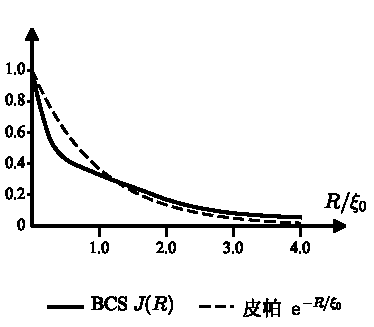
\includegraphics[width=6.5cm]{fig6-16.pdf}\\{\small 图 6.16}
\end{minipage}
\end{center}

\subsection*{5. 有限温度时的伦敦穿透深度}

在这里我们将用简单方法讨论 $T>0$ K时 $\lambda_{\mathrm{L}}(T)$ 随温度T的变化，具体计算超电流密度对弱磁场的线性响应
$\boldsymbol{j}(\boldsymbol{q},T)
=-\left(c/4\pi\right)K(q,T)\boldsymbol{A}(\boldsymbol{q})$，
并证明其系数K在伦敦极限 $\left(\boldsymbol{q}\to0\right)$ 满足
\begin{equation}
  K(q\to0,T)=\lambda_{\mathrm{L}}^{-2}(0)
  \left\{1-2\int_{\Delta}^{\infty}\mathrm{d}\xi\,
  \frac{\xi}{\sqrt{\xi^{2}-\Delta^{2}}}
  \left[-\frac{\partial f(\xi)}{\partial\xi}\right]\right\}
\end{equation}
其中 $\xi=\sqrt{\varepsilon^{2}+\Delta^{2}(T)}$，
$f(\xi)=\left[\exp\left(\beta\xi\right)+1\right]^{-1}$

首先讨论逆磁电流 $j_{2}$ 部分的贡献，根据式(6.8.11)，准至A一阶的有限温度 $j_{2}$ 在伦敦极限为
\begin{equation*}
\begin{aligned}
  \boldsymbol{j}_{2}(\boldsymbol{r},T)
  &=\langle\hat{\boldsymbol{j}}_{2}(\boldsymbol{r})\rangle_{T}\\
  &=-\frac{e^{2}}{mc}\boldsymbol{A}(\boldsymbol{r})
  \sum_{k,\,q}\mathrm{e}^{-\mathrm{i}\boldsymbol{q}\cdot\boldsymbol{r}}
  \left(\langle C^{+}_{k+q}C_{k}\rangle_{T}
  +\langle C^{+}_{-k}C_{-k-q}\rangle_{T}\right)\\
  &=-\frac{e^{2}}{mc}\boldsymbol{A}(\boldsymbol{r})
  \sum_{k}\left(\langle C^{+}_{k}C_{k}\rangle_{T}
  +\langle C^{+}_{-k}C_{-k}\rangle_{T}\right)\\
  &=-\frac{e^{2}}{mc}\boldsymbol{A}(\boldsymbol{r})\sum_{k}
  \left[1-\left(\varepsilon_{k}/\xi_{k}\right)
  \tanh\left(\frac{1}{2}\beta\xi_{k}\right)\right]
\end{aligned}
\end{equation*}
其中利用了平移对称性和习题(31)的结果.由于上式右边第二项是 $\varepsilon_{k}$ 的奇函数，它对于 $j_{2}$ 应无贡献，这时我们得到与零温情形式(6.8.12)相同的结果，再作傅里叶变换，可将其写为
\begin{equation*}
  \boldsymbol{j}_{2}(\boldsymbol{q},T)
  =-\frac{c}{4\pi}\lambda_{\mathrm{L}}^{-2}(0)\boldsymbol{A}(\boldsymbol{q})
  \equiv-\frac{c}{4\pi}K_{2}(q,T)\boldsymbol{A}(\boldsymbol{q})
\end{equation*}
表明逆磁电流的线性响应系数 $K_{2}$ 是一个与温度T和波数q均无关的量
\begin{equation}
  K_{2}(q,T)=\lambda_{\mathrm{L}}^{-2}(0)=\frac{4\pi ne^{2}}{mc^{2}}
\end{equation}
因此，总响应系数K的温度依赖只能来源于 $j_{1}$ 部分.类似于本节"1"中的讨论，取总哈密顿量
\begin{equation*}
  H=H_{0}+H_{1}
\end{equation*}
其中 $H_{0}$ 用无外磁场时系统的对角化哈密顿量式(6.4.23)表示
\begin{equation*}
  H_{0}=\sum_{k}\xi_{k}\left(\alpha^{+}_{k}\alpha_{k}
  +\alpha^{+}_{-k}\alpha_{-k}\right)+E_{\mathrm{s}}
\end{equation*}
而 $H_{1}$ 代表电子与外磁场的互作用，仍由式(6.8.8)表示.在伦敦极限 $\left(q\to0\right.$ 或 $\left.q\xi_{0}\ll1\right)$，由于式(6.8.8)等式右边第一项趋于零，而第二项的系数近似为1，这时 $H_{1}$ 可取为
\begin{equation}
  H_{1}\approx-\frac{e\hbar}{mc}\sum_{k}
  \left[\boldsymbol{k}\cdot\boldsymbol{A}(\boldsymbol{q})\right]
  \left(\alpha^{+}_{k}\alpha_{k}-\alpha^{+}_{-k}\alpha_{-k}\right)
\end{equation}
定义两种准粒子 $\alpha_{k}$ 与 $\alpha_{-k}$ 在弱外磁场中的重整化能量
\begin{equation}
  \left.
  \begin{aligned}
    \xi^{(-)}_{k}&\equiv\xi_{k}
    -\frac{e\hbar}{mc}\boldsymbol{k}\cdot\boldsymbol{A}(\boldsymbol{q})\\
    \xi^{(+)}_{k}&\equiv\xi_{k}
    +\frac{e\hbar}{mc}\boldsymbol{k}\cdot\boldsymbol{A}(\boldsymbol{q})
  \end{aligned}\right\}
\end{equation}
可将总哈密顿量H写成下列对角化的独立准粒子表示式：
\begin{equation}
  H=\sum_{k}\left(\xi^{(-)}_{k}\alpha^{+}_{k}\alpha_{k}
  +\xi^{(+)}_{k}\alpha^{+}_{-k}\alpha_{-k}\right)+E_{\mathrm{s}}
\end{equation}
再对式(6.8.13)取伦敦极限，得到
\begin{equation}
  \hat{\boldsymbol{j}}_{1}(\boldsymbol{r})\approx
  \left(\frac{e\hbar}{m}\right)\sum_{q}\mathrm{e}^{\mathrm{i}\boldsymbol{q}\cdot\boldsymbol{r}}
  \left\{\sum_{k}\boldsymbol{k}\left(\alpha^{+}_{k}\alpha_{k}
  -\alpha^{+}_{-k}\alpha_{-k}\right)\right\}
\end{equation}
其傅里叶分量
\begin{equation}
  \hat{\boldsymbol{j}}_{1}(\boldsymbol{q}\to0)\approx
  \left(\frac{e\hbar}{m}\right)\sum_{k}\boldsymbol{k}
  \left(\alpha^{+}_{k}\alpha_{k}-\alpha^{+}_{-k}\alpha_{-k}\right)
\end{equation}
与 $\boldsymbol{q}$ 无关，对上式求统计平均，并利用式(6.5.2)和式(6.8.43)可将 $j_{1}$ 的贡献表示为
\begin{equation}
\begin{aligned}
  \boldsymbol{j}_{1}(q\to0,T)&=\langle j_{1}(q\to0)\rangle\\
  &=\left(\frac{e\hbar}{m}\right)\sum_{k}\boldsymbol{k}
  \left(\langle\alpha^{+}_{k}\alpha_{k}\rangle_{T}
  -\langle\alpha^{+}_{-k}\alpha_{-k}\rangle_{T}\right)\\
  &=\left(\frac{e\hbar}{m}\right)\sum_{k}\boldsymbol{k}
  \left[f\left(\xi^{(-)}_{k}\right)-f\left(\xi^{(+)}_{k}\right)\right]
\end{aligned}
\end{equation}
由于在弱磁场时 $\xi^{(\pm)}_{k}$ 中含A项较小，可将 $f\left(\xi^{(\pm)}_{k}\right)$ 相对于 $f(\xi_{k})$ 作展开，求得
\begin{equation}
  f\left(\xi^{(-)}_{k}\right)-f\left(\xi^{(+)}_{k}\right)
  \approx-2\left[-\frac{\partial f}{\partial\xi_{k}}\right]
  \left(\frac{e\hbar}{mc}\right)
  \left[\boldsymbol{k}\cdot\boldsymbol{A}(\boldsymbol{q})\right]
\end{equation}
再代入式(6.8.46)，并将其中的缓变部分
$\boldsymbol{k}\left[\boldsymbol{k}\cdot\boldsymbol{A}(\boldsymbol{q})\right]$
用费密球面上的平均值 $\left[\dfrac{1}{3}k_{\mathrm{F}}^{2}
\boldsymbol{A}(\boldsymbol{q}\to0)\right]$ 代替，求得渐近式
\begin{equation}
\begin{aligned}
  \boldsymbol{j}_{1}(q\to0,T)
  &=\frac{2}{3}\left(\frac{e^{2}\hbar^{2}k_{\mathrm{F}}^{2}}{m^{2}c}\right)
  \boldsymbol{A}(q\to0)\sum_{k}
  \left[-\frac{\partial f(\xi_{k})}{\partial\xi_{k}}\right]\\
  &=\left\{\frac{4e^{2}E_{\mathrm{F}}}{3mc}\,g(0)\,2
  \int_{0}^{\infty}\mathrm{d}\varepsilon
  \left[-\frac{\partial f(\xi)}{\partial\xi}\right]\right\}
  \boldsymbol{A}(q\to0)\\
  &\equiv-\frac{c}{4\pi}K_{1}(q\to0,T)\boldsymbol{A}(q\to0)
\end{aligned}
\end{equation}
再考虑到费密面上正常金属的态密度 $g(0)=\left(3n/4E_{\mathrm{F}}\right)$ 和 $\xi\geqslant\Delta$ 时 $\left(\mathrm{d}\varepsilon/\mathrm{d}\xi\right)
=\xi/\sqrt{\xi^{2}-\Delta^{2}}$，可将 $j_{1}$ 的响应系数写为
\begin{equation}
  K_{1}(q\to0,T)=-\frac{2}{\lambda_{\mathrm{L}}^{2}(0)}
  \int_{\Delta}^{\infty}\mathrm{d}\xi\,
  \frac{\xi}{\sqrt{\xi^{2}-\Delta^{2}}}
  \left[-\frac{\partial f(\xi)}{\partial\xi}\right]
\end{equation}
因此，在弱外磁场中有限温度时总电流密度 $\boldsymbol{j}=\boldsymbol{j}_{1}+\boldsymbol{j}_{2}$ 的线性响应系数为
\begin{equation*}
\begin{aligned}
  K(q\to0,T)&=K_{1}(q\to0,T)+K_{2}(q\to0,T)\\
  &=\lambda_{\mathrm{L}}^{-2}(0)\left\{1-2\int_{\Delta}^{\infty}
  \mathrm{d}\xi\,\frac{\xi}{\sqrt{\xi^{2}-\Delta^{2}}}
  \left[-\frac{\partial f(\xi)}{\partial\xi}\right]\right\}\\
  &\equiv\lambda_{\mathrm{L}}^{-2}(T)
\end{aligned}
\end{equation*}
式(6.8.39)得证.

如果将 $\lambda_{\mathrm{L}}^{-2}(T)$ 写成与 $\lambda_{\mathrm{L}}^{-2}(0)$ 相似的形式
\begin{equation*}
  \lambda_{\mathrm{L}}^{-2}(T)\equiv 4\pi n_{\mathrm{s}}(T)\frac{e^{2}}{mc^{2}}
\end{equation*}
又可将 $T>0$ 的伦敦穿透深度表示为
\begin{equation}
\begin{aligned}
  \frac{n_{\mathrm{s}}(T)}{n}
  &\equiv\left[\frac{\lambda_{\mathrm{L}}(0)}{\lambda_{\mathrm{L}}(T)}\right]^{2}\\
  &=1-2\beta\int_{0}^{\infty}\frac{g_{\mathrm{s}}(\omega)}{g(0)}\,
  f(\omega)\left[1-f(\omega)\right]
\end{aligned}
\end{equation}
其中 $g_{\mathrm{s}}(\omega)$ 为超导体中准粒子的态密度，对于BCS超导体，根据式(6.6.19)
\begin{equation*}
  g_{\mathrm{s}}(\omega)=g(0)\,\mathrm{Re}\,
  \frac{|\omega|}{\sqrt{\omega^{2}-\Delta^{2}}}
\end{equation*}
作为一个练习［习题(34)］，读者不难导出伦敦穿透深度的渐近式
\begin{equation}
  \left[\frac{\lambda_{\mathrm{L}}(0)}{\lambda_{\mathrm{L}}(T)}\right]^{2}
  =\begin{cases}
    \displaystyle 2\left(1-\frac{T}{T_{\mathrm{c}}}\right)
    & \left(T_{\mathrm{c}}-T\ll T_{\mathrm{c}}\right)\\[1em]
    \displaystyle 1-\sqrt{\frac{2\pi\Delta(0)}{k_{\mathrm{B}}T}}\,
    \mathrm{e}^{-\Delta(0)/k_{\mathrm{B}}T}
    & \left(T\ll T_{\mathrm{c}}\right)
  \end{cases}
\end{equation}
特别是在低温区 $\left(T\ll T_{\mathrm{c}}\right)$，上式可简化为
\begin{equation}
  \frac{\Delta\lambda}{\lambda_{\mathrm{L}}(0)}
  =\frac{\lambda_{\mathrm{L}}(T)-\lambda_{\mathrm{L}}(0)}{\lambda_{\mathrm{L}}(0)}
  \approx\sqrt{\frac{\pi\Delta(0)}{2k_{\mathrm{B}}T}}\,
  \mathrm{e}^{-\Delta(0)/k_{\mathrm{B}}T}
  \qquad(T\ll T_{\mathrm{c}})
\end{equation}
表现出在低温时 $\Delta\lambda(T)\sim\mathrm{e}^{-\beta\Delta(0)}$ 的指数激发特征，与低温比热容 $c_{\mathrm{es}}\sim\mathrm{e}^{-\beta\Delta(0)}$ 的特征相似.此外，式(6.8.50)也适用于各向异性超导体，我们将在第七章中作专门的介绍.式(6.8.50)也可以看作是有限温度超导电子浓度 $n_{\mathrm{s}}(T)$ 的定义式.当 $T=0$ K时，由于没有准粒子激发，等式右边第二项为零，得到 $n_{\mathrm{s}}(0)=n$.但是，当 $T>0$ K时，由于实际上还存在着准粒子激发 $\left(n_{\mathrm{QP}}\neq0\right)$，应有关系式 $n_{\mathrm{s}}(T)=n-n_{\mathrm{QP}}(T)$，这时式(6.8.50)等式右边第二项实际上代表比值 $n_{\mathrm{QP}}(T)/n$.因此，在 $0<T<T_{\mathrm{c}}$ 温区内，随着T升高QP的激发 $\left(n_{\mathrm{QP}}/n\right)$ 增大，相应的超导电子浓度 $n_{\mathrm{s}}(T)$ 减小，使得屏蔽磁场的超电流减弱，这就是 $\lambda_{\mathrm{L}}(T)$ 随温度上升而增大的物理原因.

\section{BCS超导体中的粒子数和相位}

以上讨论限于 $\Delta$ 为实量.在一般情况下，对势 $\Delta$ 是一个复量，我们应当设
\begin{equation}
  \left.
  \begin{aligned}
    \Delta&=V\sum_{k}\langle C_{-k}C_{k}\rangle=|\Delta|\,\mathrm{e}^{\mathrm{i}\varphi}\\
    \Delta^{*}&=V\sum_{k}\langle C^{+}_{k}C^{+}_{-k}\rangle
    =|\Delta|\,\mathrm{e}^{-\mathrm{i}\varphi}
  \end{aligned}\right\}
\end{equation}
所对应的自洽场近似（SCFA）的哈密顿量与式(6.4.6)略有不同
\begin{equation}
  \overline{H}=\sum_{k}\varepsilon_{k}
  \left(C^{+}_{k}C_{k}+C^{+}_{-k}C_{-k}\right)
  -\sum_{k}\left(\Delta C^{+}_{k}C^{+}_{-k}
  +\Delta^{*}C_{-k}C_{k}\right)+|\Delta|^{2}/V
\end{equation}
对角化的 $u$-$v$ 变换仍与式(6.4.9)相似
\begin{equation}
  \left.
  \begin{aligned}
    \alpha_{k}&=u_{k}C_{k}-v_{k}C^{+}_{-k}\\
    \alpha_{-k}&=u_{k}C_{-k}+v_{k}C^{+}_{k}
  \end{aligned}\right\}
\end{equation}
但 $u_{k}$ 与 $v_{k}$ 也应取为复量.其逆变换与式(6.4.15)则不相同
\begin{equation}
  \left.
  \begin{aligned}
    C_{k}&=u^{*}_{k}\alpha_{k}+v_{k}\alpha^{+}_{-k}\\
    C_{-k}&=u^{*}_{k}\alpha_{-k}-v_{k}\alpha^{+}_{k}
  \end{aligned}\right\}
\end{equation}
而与式(6.4.17)相应的对角化条件变为
\begin{equation}
  \Delta u_{k}^{2}-\Delta^{*}v_{k}^{2}=2\varepsilon_{k}u_{k}v_{k}
\end{equation}
其中
\begin{equation}
  |u_{k}|^{2}+|v_{k}|^{2}=1
\end{equation}
用 $\left(\Delta^{*}/u_{k}^{2}\right)$ 乘式(6.9.5)的等式两边，得到
\begin{equation}
  \left(\Delta^{*}\frac{v_{k}}{u_{k}}\right)^{2}
  +2\varepsilon_{k}\left(\Delta^{*}\frac{v_{k}}{u_{k}}\right)
  -|\Delta|^{2}=0
\end{equation}
其稳定解为
\begin{equation}
  \Delta^{*}\left(\frac{v_{k}}{u_{k}}\right)=\xi_{k}-\varepsilon_{k}
\end{equation}
其中 $\xi_{k}=\sqrt{\varepsilon_{k}^{2}+|\Delta|^{2}}$ 代表元激发能量，与取 $\Delta$ 为实量时的结果完全一样，只要记住在式(6.4.19)中 $\Delta^{2}\equiv|\Delta|^{2}=\Delta^{*}\Delta$.再利用式(6.9.6)即可求出
\begin{equation}
  \left.
  \begin{aligned}
    |u_{k}|^{2}&=\frac{1}{2}\left(1+\varepsilon_{k}/\xi_{k}\right)\\
    |v_{k}|^{2}&=\frac{1}{2}\left(1-\varepsilon_{k}/\xi_{k}\right)
  \end{aligned}\right\}
\end{equation}
也与 $u_{k}$ 和 $v_{k}$ 均为实量时的结果完全一致.注意到式(6.9.8)等式右边的量 $\left(\xi_{k}-\varepsilon_{k}\right)$ 为实量，按此 $\Delta^{*}\left(\dfrac{v_{k}}{u_{k}}\right)$ 也应是实数，于是得到
\begin{equation}
  \frac{v_{k}}{u_{k}}
  =\Delta\left[\frac{\left(\xi_{k}-\varepsilon_{k}\right)}{|\Delta|^{2}}\right]
\end{equation}
上式表明 $v_{k}$ 相对于 $u_{k}$ 的相位与能隙 $\Delta$ 的相位相同，这是一个重要的结果.

BCS超导体的基态波函数仍可写成式(6.4.38)的形式，只是现在 $u_{k}$ 与 $v_{k}$ 应为复量.由于在量子力学中允许总波函数相差一个相位因子，我们可以进一步设 $u_{k}$ 为实，而仅取 $v_{k}$ 为复量
\begin{equation}
  u_{k}=|u_{k}|\text{，}
  \qquad v_{k}=|v_{k}|\,\mathrm{e}^{\mathrm{i}\varphi_{k}}
\end{equation}
这时 $\varphi_{k}$ 正好代表 $v_{k}$ 相对于 $u_{k}$ 的相位差，再根据式(6.9.10)和式(6.9.1)可以求出
\begin{equation}
  \varphi_{k}=\varphi
\end{equation}
这是一个非常重要的结果，它表明：在BCS超导体中在任一 $(\boldsymbol{k}\uparrow,-\boldsymbol{k}\downarrow)$ 态上被一对电子占据时的概率幅 $v_{k}$ 的相位差是与k无关的一个常数.换句话说，所有在费密面附近凝聚的电子对都具有相同的相位差 $\varphi$.在这个意义上，人们常说BCS的超导基态是一种相位相干态.这时基态波函数应写为
\begin{equation}
  |\varphi\rangle=\prod_{k}
  \left(|u_{k}|+|v_{k}|\,\mathrm{e}^{\mathrm{i}\varphi}
  C^{+}_{k}C^{+}_{-k}\right)|\mathrm{VAC}\rangle
\end{equation}
其中 $\varphi$ 可取0到 $2\pi$ 之间的任一确定值.显然，前面的式(6.4.38)代表 $\varphi=0$ 的特殊相位情形，并且 $u_{k}=|u_{k}|$，$v_{k}=|v_{k}|$.在一般情况下，最好保留 $\varphi$ 而写成在(6.9.13)的形式，因为由此可导出粒子数与相位之间的不确定关系.

仔细考察式(6.9.13)，不难发现在 $|\varphi\rangle$ 中粒子数N严格确定的状态 $|N\rangle$ 是其乘积展开式中含有 $\dfrac{N}{2}$ 个 $\mathrm{e}^{\mathrm{i}\varphi}$ 因子的项，根据安德逊的做法，可以通过下面的相位积分取出 $|\varphi\rangle$ 中含N个粒子状态的分量
\begin{equation}
  |N\rangle=\frac{1}{2\pi}\int_{0}^{2\pi}\mathrm{d}\varphi\,
  \mathrm{e}^{-\mathrm{i}N\varphi/2}|\varphi\rangle
\end{equation}
上式中对相位 $\varphi$ 的所有可能取值作积分，也就是使相位 $\varphi$ 完全不确定，这时我们才可以得到完全确定粒子数N的状态，而其逆变换为
\begin{equation}
  |\varphi\rangle=\sum_{N=0}^{\infty}\mathrm{e}^{\mathrm{i}N\varphi/2}|N\rangle
\end{equation}
从物理上讲，确定的相位 $\varphi$，对应于总粒子数不守恒的情况，这是BCS基态波函数的一个重要特征.显然，$|N\rangle$ 和 $|\varphi\rangle$ 之间的变换关系与量子力学中共轭量 $\boldsymbol{p}$ 和x之间的本征函数 $|\boldsymbol{p}\rangle$ 和 $|\boldsymbol{x}\rangle$ 的变换关系相似.可以认为N与 $\varphi$ 也是一对共轭力学量，并且可将 $\dfrac{N}{2}$ 对应于 $\boldsymbol{p}$，$\hbar\varphi$ 对应于x，再根据不确定关系式
$\Delta p\,\Delta x\geqslant\dfrac{\hbar}{2}$，求出N与 $\varphi$ 间相应的不确定关系
\begin{equation}
  \Delta N\,\Delta\varphi\gtrsim1
\end{equation}
它同样地反映了系统的量子特性，表明同时测量N和 $\varphi$ 的精度有一个限制.

现在我们转入对BCS超导体中确定粒子数和相位的精度作定性的讨论.在BCS超导基态中的平均粒子数 $\overline{N}$ 由粒子数算符
$\hat{N}=\sum_{k}\left(C^{+}_{k}C_{k}+C^{+}_{-k}C_{-k}\right)$
的基态平均决定，当取 $\varphi=0$ 时，习题(30)中已证明
\begin{equation}
  \overline{N}=\langle0|\hat{N}|0\rangle
  =2\sum_{k}v_{k}^{2}
  =\frac{\Omega}{(2\pi)^{3}}\int\mathrm{d}^{3}k\,\left(2v_{k}^{2}\right)
\end{equation}
而其均方涨落也已求出为
\begin{equation}
  \langle\hat{N}^{2}\rangle-\langle\hat{N}\rangle^{2}
  =\sum_{k}4u_{k}^{2}v_{k}^{2}
  =\frac{\Omega}{(2\pi)^{3}}\int\mathrm{d}^{3}k\,
  \left(4u_{k}^{2}v_{k}^{2}\right)
\end{equation}
在这里 $\Omega$ 代表样品的体积.在热力学极限（当 $\overline{N}\to\infty$ 和 $\Omega\to\infty$，但两者比值固定时），可根据均方涨落正比于体积 $\Omega$，断定它必然正比于 $\overline{N}$.按此求出均方根涨落，即 $\Delta N$ 为
\begin{equation}
  \Delta N=\sqrt{\langle(\hat{N}-\overline{N})^{2}\rangle}
  =\sqrt{\langle\hat{N}^{2}\rangle-\overline{N}^{2}}
  \approx\overline{N}^{1/2}
\end{equation}
由于 $\overline{N}\sim10^{20}$，可取 $\Delta N\sim10^{10}$，代入不确定关系式(6.9.16)，求得 $\varphi=0$ 时的位相涨落 $\Delta\varphi\sim10^{-10}$ 是一个很小的量，说明BCS超导体中相位涨落很小.另一方面，尽管均方根涨落 $\Delta N$ 较大，但在BCS基态中粒子数的相对涨落
$\left(\dfrac{\Delta N}{\overline{N}}\right)\sim\dfrac{1}{\overline{N}^{1/2}}
\sim10^{-10}$ 却是很小的.换句话说，在BCS基态中 $\left(\Delta N/\overline{N}\right)$ 和 $\Delta\varphi$ 都近似在 $\overline{N}^{-1/2}\sim10^{-10}$ 的数量级范围内可被确定.

以上讨论表明：BCS超导体中相位 $\varphi$ 与粒子数N是一对共轭力学量，满足不确定关系式(6.9.16).另一方面，允许 $\varphi$ 取特定值（包括在本章§4中取 $\varphi=0$ 情形）则对应于BCS超导体中的相位相干和总粒子数不守恒等两项重要特性.在空间非均匀情况下，当涉及两块超导体的连接系统时，对势 $\Delta$ 中所含相位因子 $\mathrm{e}^{\mathrm{i}\varphi}$ 将起重要的作用，涉及库柏对在两块弱连接超导体间的隧穿问题.我们将在下一节中采用唯象的金兹堡-朗道理论对超导体中的相位相干特征作进一步的探讨，涉及超导体中的约瑟夫森效应.

\section{金兹堡-朗道方程}

在伦敦方程中，超导电子密度与磁场及空间位置无关，因此它只适用于讨论弱磁场中的均匀超导体问题，而不能处理非均匀超导体（如超导体与正常体的S-N界面等问题）和强磁场情况.为计及超导电子密度随空间位置的变化，金兹堡和朗道\textsuperscript{[9]}（后简称G-L）建议用一个复量 $\psi(\boldsymbol{r})$ 作为超导电子的"有效波函数"，$\psi(\boldsymbol{r})$ 与超导电子的局域密度 $n_{\mathrm{s}}(\boldsymbol{r})$ 有如下关系：
\begin{equation}
  |\psi(\boldsymbol{r})|^{2}=n_{\mathrm{s}}(\boldsymbol{r})
\end{equation}
对于正常态 $n_{\mathrm{s}}=0$，$\psi=0$，而超导态 $n_{\mathrm{s}}\neq0$，$\psi\neq0$.因此 $\psi$ 起序参数作用，这是一个复序参数.由于超导-正常转变是二级相变，$T\to T_{\mathrm{c}}$ 时 $n_{\mathrm{s}}\to0$，在转变点附近 $\psi$ 应为小量，可以将自由能展开为序参量 $|\psi|^{2}$ 的幂级数，并计及磁场 $\boldsymbol{B}=\nabla\times\boldsymbol{A}$ 的影响，利用自由能泛函的极小确定空间各点的序参数方程和电流密度方程（G-L方程），这就是金兹堡-朗道唯象理论的基本精神.理论主要用于 $T_{\mathrm{c}}-T\ll T_{\mathrm{c}}$ 温区.

\subsection*{1. G-L自由能}

对于均匀超导体，当外场为零时在 $T_{\mathrm{c}}$ 附近自由能密度 $f_{\mathrm{s}}$ 可按小量 $n_{\mathrm{s}}$ 展开
\begin{equation*}
  f_{\mathrm{s}}=f_{\mathrm{n}}+\alpha(T)n_{\mathrm{s}}
  +\frac{1}{2}\beta(T)n_{\mathrm{s}}^{2}+\cdots
\end{equation*}
略去高阶项，并利用式(6.10.1)将上式改写成序参量的展式
\begin{equation}
  f_{\mathrm{s}}=f_{\mathrm{n}}+\alpha(T)|\psi(\boldsymbol{r})|^{2}
  +\frac{1}{2}\beta(T)|\psi(\boldsymbol{r})|^{4}
\end{equation}
其中 $f_{\mathrm{n}}$ 为零磁场时正常态的自由能密度.$\alpha$、$\beta$ 是与温度有关的唯象参数，可利用自由能极小定出
\begin{equation}
  n_{\mathrm{s}}=|\psi(\boldsymbol{r})|^{2}
  =-\frac{\alpha(T)}{\beta(T)}
\end{equation}
由于 $T<T_{\mathrm{c}}$ 时 $n_{\mathrm{s}}>0$，因此式(6.10.3)要求 $\left(\alpha/\beta\right)<0$，将式(6.10.3)代入式(6.10.2)，得
\begin{equation}
  f_{\mathrm{n}}-f_{\mathrm{s}}=\frac{1}{2}\frac{\alpha^{2}(T)}{\beta(T)}
  =\frac{1}{8\pi}H_{\mathrm{c}}^{2}(T)
\end{equation}
最后一个等式中的 $H_{\mathrm{c}}(T)$ 是破坏超导的临界磁场，这里利用了熟知的超导热力学关系，式(6.10.4)要求 $\beta(T)>0$.又因为 $T=T_{\mathrm{c}}$ 时 $n_{\mathrm{s}}=0$，从公式(6.10.3)还可得知 $\alpha(T_{\mathrm{c}})=0$ 和 $\beta(T_{\mathrm{c}})\neq0$，因此在 $T_{\mathrm{c}}-T\ll T_{\mathrm{c}}$ 温区，$\alpha$、$\beta$ 可表示成
\begin{equation}
  \left.
  \begin{aligned}
    \alpha(T)&=\left(T-T_{\mathrm{c}}\right)
    \left(\frac{\mathrm{d}\alpha}{\mathrm{d}T}\right)_{T_{\mathrm{c}}}\\
    \beta(T)&\approx\beta\left(T_{\mathrm{c}}\right)
  \end{aligned}\right\}
\end{equation}
由式(6.10.4)与式(6.10.5)，得 $f_{\mathrm{n}}-f_{\mathrm{s}}\sim\left(T_{\mathrm{c}}-T\right)^{2}$.因此，$H_{\mathrm{c}}\sim\left(T_{\mathrm{c}}-T\right)$，与实验相符，并反映了转变点附近二级相变的共同特征.

式(6.10.2)只是均匀超导体的朗道二级相变公式.假如 $\psi$ 随位置 $\boldsymbol{r}$ 变化，还需在式(6.10.2)中计入 $\psi$ 的导数项对 $f_{\mathrm{s}}$ 的影响.当 $|\psi|^{2}$ 变化缓慢时，G-L取磁场矢量 $\boldsymbol{A}=0$ 时的附加能量为
\begin{equation*}
  \frac{1}{2m^{*}}\left|-\mathrm{i}\hbar\nabla\psi(\boldsymbol{r})\right|^{2}
\end{equation*}
与有效质量为 $m^{*}$，波函数为 $\psi$ 的"粒子"的动能项相似.物理上可理解为 $\boldsymbol{A}=0$ 时，$\nabla\psi\neq0$，对应于超导体的载流状态，因此有上述类似动能项出现.

推广到 $\boldsymbol{A}(\boldsymbol{r})\neq0$ 情况，可根据电动力学将 $-\mathrm{i}\hbar\nabla$ 换成为正则动量 $-\mathrm{i}\hbar\nabla-\dfrac{e^{*}}{c}\boldsymbol{A}$，则自由能密度的附加项为
\begin{equation*}
  \frac{1}{2m^{*}}\left|\left(-\mathrm{i}\hbar\nabla
  -\frac{e^{*}}{c}\boldsymbol{A}\right)\psi(\boldsymbol{r})\right|^{2}
\end{equation*}
好像电荷为 $e^{*}$、质量为 $m^{*}$ 的粒子在磁场中运动的动能项.这是G-L理论中的主要假定.再计及磁场能量 $\dfrac{1}{8\pi}|\nabla\times\boldsymbol{A}|^{2}$，即得G-L的自由能展开式
\begin{equation}
\begin{aligned}
  f_{\mathrm{s}}&=f_{\mathrm{n}}+\alpha(T)|\psi(\boldsymbol{r})|^{2}
  +\frac{1}{2}\beta(T)|\psi(\boldsymbol{r})|^{4}\\
  &\quad+\frac{1}{8\pi}\left(\nabla\times\boldsymbol{A}\right)
  \cdot\left(\nabla\times\boldsymbol{A}\right)
  +\frac{1}{2m^{*}}\left|\left(-\mathrm{i}\hbar\nabla
  -\frac{e^{*}}{c}\boldsymbol{A}\right)\psi(\boldsymbol{r})\right|^{2}
\end{aligned}
\end{equation}
系统的自由能为
\begin{equation}
  F_{\mathrm{s}}=\int f_{\mathrm{s}}\,\mathrm{d}\boldsymbol{r}
\end{equation}

\subsection*{2. G-L方程}

利用热力学平衡条件，要求自由能对序参数和磁场矢量势的任意变化 $\delta\psi$、$\delta\psi^{*}$ 及 $\delta\boldsymbol{A}$ 为极小，可求出G-L方程.根据式(6.10.6)与(6.10.7)，求得自由能的变分为
\begin{equation}
\begin{aligned}
  \delta F_{\mathrm{s}}&=\delta\int f_{\mathrm{s}}\,\mathrm{d}\boldsymbol{r}\\
  &=\int\mathrm{d}\boldsymbol{r}\biggl\{\delta\psi^{*}
  \left[\alpha\psi+\beta|\psi|^{2}\psi
  +\frac{1}{2m^{*}}\left(-\mathrm{i}\hbar\nabla
  -\frac{e^{*}}{c}\boldsymbol{A}\right)^{2}\psi\right]
  +\mathrm{c.c.}\biggr\}+\\
  &\quad\int\mathrm{d}\boldsymbol{r}\biggl\{\delta\boldsymbol{A}\cdot
  \left[\frac{\nabla\times\nabla\times\boldsymbol{A}}{4\pi}
  +\frac{\mathrm{i}\hbar e^{*}}{2m^{*}c}
  \left(\psi^{*}\nabla\psi-\psi\nabla\psi^{*}\right)\right.\\
  &\quad\left.+\left(\frac{e^{*}}{c}\right)^{2}
  \frac{1}{m^{*}}\boldsymbol{A}\,|\psi|^{2}\right]+\mathrm{c.c.}\biggr\}
\end{aligned}
\end{equation}
其中 $\mathrm{c.c.}$ 代表复共轭项.在推导式(6.10.8)过程中还假设了下列面积分为零
\begin{equation*}
  \int_{\mathrm{s}}\mathrm{d}S\left\{\delta\psi^{*}
  \left(-\mathrm{i}\hbar\nabla-\frac{e^{*}}{c}\boldsymbol{A}\right)_{n}\psi
  +\mathrm{c.c.}\right\}=0
\end{equation*}
下标n表示垂直表面方向的分量，相当于一个边界条件
\begin{equation}
  \left(-\mathrm{i}\hbar\nabla-\frac{e^{*}}{c}\boldsymbol{A}\right)_{n}
  \psi(\boldsymbol{r})=0
\end{equation}
要求 $\delta F_{\mathrm{s}}=0$，由式(6.10.8)可得下列方程：
\begin{equation}
  \frac{1}{2m^{*}}\left(-\mathrm{i}\hbar\nabla
  -\frac{e^{*}}{c}\boldsymbol{A}\right)^{2}\psi
  +\alpha\psi+\beta|\psi|^{2}\psi=0
\end{equation}
\begin{equation}
  \boldsymbol{j}=\frac{c}{4\pi}\nabla\times\boldsymbol{B}
  =-\frac{\mathrm{i}\hbar e^{*}}{2m^{*}}
  \left(\psi^{*}\nabla\psi-\psi\nabla\psi^{*}\right)
  -\frac{\left(e^{*}\right)^{2}}{m^{*}c}|\psi|^{2}\boldsymbol{A}
\end{equation}
这就是著名的金斯堡-朗道（G-L）方程.式(6.10.10)类似粒子在磁场中运动的薛定谔方程，但应注意它是非线性的，是确定序参数 $\psi$ 的方程.式(6.10.11)就是量子力学的电流密度公式.

\subsection*{3. G-L参数 $\kappa$}

G-L方程是非线性的联立方程，其一般解相当复杂，这里仅介绍一些简单解，主要目的是引入特征参量 $\xi(T)$、$\lambda(T)$ 和 $\kappa(T)$.

（i）序参数的空间变化范围 $\xi(T)$

G-L方程有如下两个最简单的解.

（1）$\psi=0$，而A仅仅由 $\boldsymbol{B}=\nabla\times\boldsymbol{A}$ 决定，$\boldsymbol{B}=\boldsymbol{H}$ 为外场，这个解描述正常态.

（2）$\psi=\psi_{0}=\left[-\alpha(T)/\beta(T)\right]^{\frac{1}{2}}$ 和 $\boldsymbol{A}=0$.这个解代表具有完全迈斯纳效应（忽略表面效应）的超导状态.$\psi_{0}$ 是与 $\boldsymbol{r}$ 无关的空间均匀解，这时系统具有最低自由能 $\left(T<T_{\mathrm{c}}\right.$，$\left.\alpha<0\right.$ 时$)$，如式(6.10.4).因此，人们常常说无外场时大块超导体的平衡态为序参数 $\psi=\psi_{0}=$ 常数\footnote{确切地说，$\psi_{0}$ 只是大块超导样品远离界面处的序参数值.}.

现在讨论磁场非常弱的情况，根据(2)不难预料 $\psi$ 的空间变化将十分缓慢.$\psi$ 与 $\psi_{0}$ 很接近，在G-L的第一个方程(6.10.10)中可令 $\boldsymbol{A}=0$，再引入量纲为1的序参数
\begin{subequations}
\begin{equation}
  f\equiv\frac{\psi}{\psi_{0}}\text{，}
  \qquad \psi_{0}=\sqrt{\frac{|\alpha|}{\beta}}
\end{equation}
其中f满足方程
\begin{equation}
  -\frac{\hbar^{2}}{2m^{*}\alpha}\nabla^{2}f+f-f^{3}=0
\end{equation}
\end{subequations}
由上式可定义一个特征长度 $\xi(T)$
\begin{equation}
  \xi^{2}(T)\equiv-\frac{\hbar^{2}}{2m^{*}\alpha(T)}
\end{equation}
它代表序参数（f及 $\psi$）的空间变化尺度.为了更清楚地说明 $\xi(T)$ 的性质，我们考虑以 $z=0$ 为界的N-S问题 $\left(z<0\right.$ 为正常体N，$z>0$ 为超导体S$)$.这时式(6.10.12b)简化为
\begin{equation}
  \xi^{2}\frac{\mathrm{d}^{2}f}{\mathrm{d}z^{2}}=-f\left(1-f^{2}\right)
  \qquad(z\geqslant0)
\end{equation}
边界条件为 $z=0$ 时，序参数 $f=0$.上式乘 $\left(\mathrm{d}f/\mathrm{d}z\right)$ 后积分，得出
\begin{equation}
  \xi^{2}\left(\frac{\mathrm{d}f}{\mathrm{d}z}\right)^{2}
  =\frac{1}{2}\left(1-f^{2}\right)^{2}
\end{equation}
这里积分常数由 $f^{2}\to1$ 时 $\mathrm{d}f/\mathrm{d}z\to0$ 决定.由于z增大时f增大，上式取正根
$\dfrac{\mathrm{d}f}{\mathrm{d}z}=\dfrac{1-f^{2}}{\sqrt{2}\,\xi(T)}$，求得
\begin{equation}
  f(z)=\tanh\frac{z}{\sqrt{2}\,\xi(T)}
  \qquad(z\geqslant0)
\end{equation}
由此可见，$f(z)$ 的空间变化范围是 $\xi(T)$，这个量称为G-L相干长度，它和温度的关系为
\begin{equation}
  \xi(T)=\frac{\hbar}{\left[2m^{*}\left(T_{\mathrm{c}}-T\right)
  \alpha'\left(T_{\mathrm{c}}\right)\right]^{1/2}}
\end{equation}
其中 $\alpha'\left(T_{\mathrm{c}}\right)=\left(\dfrac{\mathrm{d}\alpha}{\mathrm{d}T}\right)_{T_{\mathrm{c}}}$.当 $T\to T_{\mathrm{c}}$ 时，$\xi(T)\to\infty$.注意，$\xi(T)$ 与BCS相干长度 $\xi_{0}=\dfrac{\hbar v_{\mathrm{F}}}{\pi\Delta(0)}$ 不是同一个量.图6.17中实线表示在N-S界面序参数的变化曲线，而虚线代表磁场的穿透情况.

（ii）弱场穿透深度 $\lambda(T)$

G-L第二方程(6.10.11)在准至磁场一阶时可用无磁场时的 $\psi_{0}^{2}$ 代替其中的 $|\psi|^{2}$，从而求得电流密度j为
\begin{equation}
  \boldsymbol{j}=-\frac{\mathrm{i}\hbar e^{*}}{2m^{*}}
  \left(\psi^{*}\nabla\psi-\psi\nabla\psi^{*}\right)
  -\frac{\left(e^{*}\right)^{2}}{m^{*}c}\psi_{0}^{2}\boldsymbol{A}
\end{equation}
若令 $\psi=\psi_{0}+\psi_{1}$，$\psi_{1}$ 为含A一阶的序参量，由于 $\psi_{0}$ 与 $\boldsymbol{r}$ 无关，上式右边第一项最低阶是 $\boldsymbol{A}^{2}$ 项.因此，准至A一阶的电流公式为
\begin{equation}
\begin{aligned}
  \boldsymbol{j}(\boldsymbol{r})
  &=-\frac{\left(e^{*}\right)^{2}}{m^{*}c}\psi_{0}^{2}\boldsymbol{A}(\boldsymbol{r})\\
  &=-\frac{c}{4\pi}\left[\frac{4\pi\left(e^{*}\right)^{2}\psi_{0}^{2}}
  {m^{*}c^{2}}\right]\boldsymbol{A}(\boldsymbol{r})
\end{aligned}
\end{equation}
与伦敦方程式(6.7.8)相比较，求得穿透深度
\begin{equation}
  \lambda(T)=\left[\frac{m^{*}c^{2}}
  {4\pi\left(e^{*}\right)^{2}\psi_{0}^{2}}\right]^{1/2}
\end{equation}
再利用式(6.10.12a)和式(6.10.5)，可将 $\lambda(T)$ 表示为
\begin{equation}
  \lambda(T)=\left[\frac{m^{*}c^{2}\beta\left(T_{\mathrm{c}}\right)}
  {4\pi\left(e^{*}\right)^{2}\left(T_{\mathrm{c}}-T\right)
  \alpha'\left(T_{\mathrm{c}}\right)}\right]^{1/2}
\end{equation}
显然，在 $T_{\mathrm{c}}-T\ll T_{\mathrm{c}}$ 温区内，$\lambda(T)$ 与G-L相干长度的表示式(6.10.17)相似，它们都与 $\left(T_{\mathrm{c}}-T\right)^{-1/2}$ 成正比，并且 $\lambda(T)$ 与 $\xi(T)$ 的比值是一个与温度无关的特性常数 $\kappa$
\begin{equation}
  \kappa\equiv\frac{\lambda(T)}{\xi(T)}
  =\frac{m^{*}c}{\hbar e^{*}}\left(\frac{\beta}{2\pi}\right)^{1/2}
\end{equation}
称为G-L参数.利用 $\psi_{0}^{2}=\dfrac{|\alpha|}{\beta}$ 和式(6.10.4)，有
$|\alpha|\psi_{0}^{2}=\dfrac{1}{4\pi}H_{\mathrm{c}}^{2}(T)$，
再利用式(6.10.13)与式(6.10.20)，我们还可以将 $\kappa$ 表示为
\begin{equation}
  \kappa=\frac{\sqrt{2}\,e^{*}}{\hbar c}H_{\mathrm{c}}(T)\lambda^{2}(T)
\end{equation}
说明G-L参数 $\kappa$ 可由测量直接决定.再考虑到 $\kappa=\lambda(T)/\xi(T)$，我们又可求得诸特征量 $H_{\mathrm{c}}(T)$、$\lambda(T)$ 和 $\xi(T)$ 之间的一个重要关系式
\begin{equation}
  H_{\mathrm{c}}(T)\lambda(T)\xi(T)
  =\frac{1}{2\pi\sqrt{2}}\left(\frac{2\pi\hbar c}{e^{*}}\right)
\end{equation}
即三者的乘积为一常数，其中 $\left(2\pi\hbar c/e^{*}\right)$ 正是下面将要介绍的超导磁通量子.

G-L参数 $\kappa$ 是超导体分类的重要参数.根据图6.17在正常与超导物质之间存在着由N到S的过渡层.在过渡层中磁场连续下降为零.序参数 $\psi$ 则由零连续上升到S区深部的数值 $\psi_{0}$，这就是N-S界面区.由于磁场透入界面区和序参数在界面区下降所引起单位面积吉布斯自由能的变化称为界面能.界面能与 $\xi(T)$ 和 $\lambda(T)$ 的相对大小有关，与超导体的特征密切相关.

\begin{center}
\begin{minipage}{8cm}
\centering
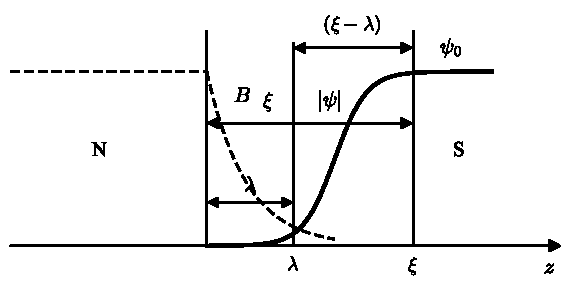
\includegraphics[width=8cm]{fig6-17.pdf}\\{\small 图 6.17\quad N-S界面区的有序参数变化}
\end{minipage}
\end{center}

为估计界面能的大小，可以将图6.17近似看作磁场 $H_{\mathrm{c}}$ 完全透入到 $0<z<\lambda(T)$ 区域，而在 $z\geqslant\lambda(T)$ 区近似为零.有序参数 $\psi$ 的变化也可当作在 $0<z<\xi(T)$ 范围内近似取零值，而在 $z\geqslant\xi(T)$ 区取 $\psi_{0}$ 值.这样，在 $\lambda<z<\xi$ 区域内序参数 $\psi$ 和B均为零，相当于无外场时的正常态，其吉布斯自由能密度显然应比纯超导态高 $H_{\mathrm{c}}^{2}/8\pi$.由于这个区域的存在所引起单位面积自由能的改变为
\begin{equation*}
  \left(\xi-\lambda\right)\frac{H_{\mathrm{c}}^{2}}{8\pi}
\end{equation*}
在 $0<z<\lambda(T)$ 区内，虽然也从原来的超导态变成了正常态，自由能密度将增加 $H_{\mathrm{c}}^{2}/8\pi$，但是由于磁场 $H_{\mathrm{c}}$ 的完全透入，吉布斯自由能密度将减少同一数值，因此 $0<z<\lambda(T)$ 区域相对于原来的纯超导态能量没有变化.于是，N-S的界面能大致为
\begin{equation}
  \sigma_{\mathrm{ns}}\approx\left(\xi-\lambda\right)\frac{H_{\mathrm{c}}^{2}}{8\pi}
\end{equation}
当 $\xi>\lambda$ 时 $\sigma_{\mathrm{ns}}>0$，界面能为正，而当 $\xi<\lambda$ 时 $\sigma_{\mathrm{ns}}<0$，界面能为负，分别属于两种不同类型的超导体.若用G-L方程严格计算界面能\textsuperscript{[10]}，可求得比式(6.10.25)更精确的结果；当 $\kappa=1/\sqrt{2}$ 时 $\sigma_{\mathrm{ns}}=0$，而
\begin{equation*}
  \kappa<\frac{1}{\sqrt{2}}\text{，}\qquad \sigma_{\mathrm{ns}}>0
  \qquad\text{（Ⅰ类超导体）}
\end{equation*}
\begin{equation*}
  \kappa>\frac{1}{\sqrt{2}}\text{，}\qquad \sigma_{\mathrm{ns}}<0
  \qquad\text{（Ⅱ类超导体）}
\end{equation*}
$\kappa<1/\sqrt{2}$ 的超导材料，具有正界面能，磁场若透入超导体必将在样品内部产生正常区，从而形成N-S界面，但由于 $\sigma_{\mathrm{ns}}>0$ 在能量上是不利的，因此Ⅰ类超导体在 $H<H_{\mathrm{c}}$ 时序参数保持均匀分布，磁场不能透入内部，样品具有完全逆磁性.当 $\kappa>1/\sqrt{2}$ 时，情况相反，在一定条件下，磁场能透入样品内部，形成许多正常区，因为这时 $\sigma_{\mathrm{ns}}<0$，界面增加在能量上是有利的.这类材料称为Ⅱ类超导体，它不具有完全逆磁性.

\subsection*{4. 磁通量子化}

从G-L的超导电流方程(6.10.11)可以证实伦敦的磁通量子化假定.将复序参数写成
\begin{equation*}
  \psi=|\psi|\,\mathrm{e}^{\mathrm{i}\varphi}
\end{equation*}
形式，$\varphi$ 为实量，代入式(6.10.11)求得
\begin{equation}
  \boldsymbol{j}=\frac{e^{*}\hbar}{m^{*}}|\psi|^{2}\nabla\varphi
  -\frac{\left(e^{*}\right)^{2}|\psi|^{2}}{m^{*}c}\boldsymbol{A}
\end{equation}
或
\begin{equation}
  \boldsymbol{A}+\frac{\boldsymbol{j}m^{*}c}{\left(e^{*}\right)^{2}|\psi|^{2}}
  =\frac{\hbar c}{e^{*}}\nabla\varphi
\end{equation}
对上式沿回路C作路径积分
\begin{equation}
  \oint_{C}\mathrm{d}\boldsymbol{l}\cdot\boldsymbol{A}
  +\frac{m^{*}c}{\left(e^{*}\right)^{2}}\oint_{C}
  \frac{\mathrm{d}\boldsymbol{l}\cdot\boldsymbol{j}}{|\psi|^{2}}
  =\frac{\hbar c}{e^{*}}\oint_{C}\mathrm{d}\boldsymbol{l}\cdot\nabla\varphi
\end{equation}
由于超导体中序参数 $\psi(\boldsymbol{r})$ 应为单值函数，因此要求绕回路C一周后 $\varphi$ 的增量
$\oint_{C}\mathrm{d}\boldsymbol{l}\cdot\nabla\varphi$ 只能取 $2\pi$ 的整倍数，再利用斯托克斯（Stokes）定理，将上式左边第一项改写成对回路C所包含面积S的面积分
$\oint_{C}\mathrm{d}\boldsymbol{l}\cdot\boldsymbol{A}
=\int_{S}\mathrm{d}\boldsymbol{S}\cdot\left(\nabla\times\boldsymbol{A}\right)
=\int_{S}\boldsymbol{B}\cdot\mathrm{d}\boldsymbol{S}$，求得
\begin{equation}
  \int_{S}\boldsymbol{B}\cdot\mathrm{d}\boldsymbol{S}
  +\frac{m^{*}c}{\left(e^{*}\right)^{2}}\oint
  \frac{\mathrm{d}\boldsymbol{l}\cdot\boldsymbol{j}}{|\psi|^{2}}
  =n\frac{2\pi\hbar c}{e^{*}}
\end{equation}
如果积分回路取在没有超电流的地方，则左边第二项积分等于零，就得到磁通量子化的结果为
\begin{equation}
  \Phi=\int_{S}\boldsymbol{B}\cdot\mathrm{d}\boldsymbol{S}
  =n\frac{2\pi\hbar c}{e^{*}}\equiv n\Phi_{0}
  \qquad(n=\text{整数})
\end{equation}
$\Phi_{0}=\dfrac{2\pi\hbar c}{e^{*}}$ 称为磁通量子，这个结果已为实验所证实\textsuperscript{[11]}.实验测得的磁通量子
\begin{equation}
  \Phi_{0}=\frac{2\pi\hbar c}{2e}=2.07\times10^{-7}\,\mathrm{Gs\cdot cm^{2}}
\end{equation}
因此
\begin{equation}
  e^{*}=2e
\end{equation}
说明超电流是电子对运动所导致的.这个实验也直接证实了超导体中库柏对的存在.

图6.18(a)和(b)分别表示单连通和复连通的Ⅰ类超导体中的回路C.对于图(a)，磁通量子数取 $n=0$，表示磁通不通透入单连通超导体内部.对于图(b)，n取整数.图形(c)表示超导体内有正常态的小圆柱区情况，这时n也可取整数，相当于Ⅱ类超导体中形成正常区，属于有磁力线穿透情况（称为混合态）.阿布里科索夫（Abrikosov）\textsuperscript{[12]}严格解G-L方程证明了这时可出现许多细状的正常区，并排成阵列，在每个正常区内可穿透一个磁通量子的磁力线——量子磁通线.

最后，简单介绍G-L复序参量和BCS微观理论的关系，从微观角度讲，超导序和库柏对的形成有关，能隙 $\Delta$ 随温度的变化实际上反映了序参数的变化 $\left(T<T_{\mathrm{c}}\right.$ 时 $\Delta\neq0$，$T\geqslant T_{\mathrm{c}}$ 时 $\Delta=0\left.\right)$.根据式(6.5.1)，均匀超导体的能隙定义为
\begin{equation*}
  \Delta=V\sum_{k}\langle C_{-k}C_{k}\rangle_{T}
  =V\sum_{k}u_{k}v_{k}\left[1-2f(\xi_{k})\right]
\end{equation*}
是与位置 $\boldsymbol{r}$ 无关的常量，其中根据式(6.9.11)和式(6.9.12)，因子
$u_{k}v_{k}=u_{k}|v_{k}|\,\mathrm{e}^{\mathrm{i}\varphi}$ 含有一个常数相位 $\varphi$，代表费密面附近所有凝聚电子对的共同相位.因此，即使在空间均匀情况下超导体中的能隙参数 $\Delta$ 也应当用一个复数的常量 $|\Delta|\,\mathrm{e}^{\mathrm{i}\varphi}$ 描述.推广到空间非均匀情形，我们可以利用场量 $\Psi_{\uparrow}(\boldsymbol{r})$ 与 $\Psi_{\downarrow}(\boldsymbol{r})$，定义与一个 $\boldsymbol{r}$ 有关的能隙函数

\begin{center}
\begin{minipage}{9.5cm}
\centering
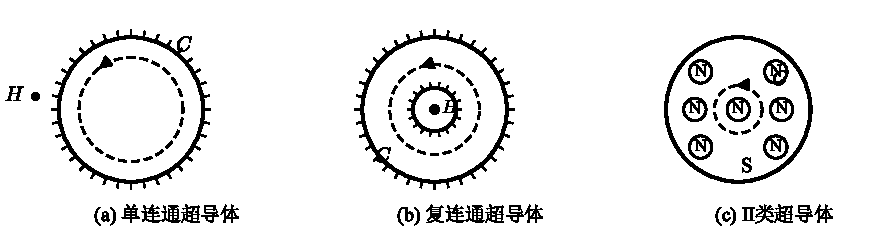
\includegraphics[width=9.5cm]{fig6-18.pdf}\\[0.3em]
{\small (a) 单连通超导体\qquad (b) 复连通超导体\qquad (c) Ⅱ类超导体}\\[0.2em]
{\small 图 6.18}
\end{minipage}
\end{center}

\begin{equation}
  \Delta(\boldsymbol{r})=V\langle\Psi_{\downarrow}(\boldsymbol{r})
  \Psi_{\uparrow}(\boldsymbol{r})\rangle
\end{equation}
将上式中场量 $\Psi_{\sigma}(\boldsymbol{r})$ 用平面波展开，对于空间均匀情形，利用平移不变性，仍可以求得超导的能隙函数与位置无关.一般情况下，$\Delta(\boldsymbol{r})$ 显然是一个与位置 $\boldsymbol{r}$ 有关的复量，$\Delta(\boldsymbol{r})$ 相当于G-L的复有序参量 $\psi(\boldsymbol{r})$.戈尔柯夫（Gorkov）用格林函数方法首先证明了 $\Delta(\boldsymbol{r})$ 所满足的方程与G-L方程相同，G-L的序参量 $\psi(\boldsymbol{r})$ 与能隙函数成正比\textsuperscript{[10]}
\begin{equation}
  \psi(\boldsymbol{r})=\frac{\left[7\zeta(3)\,n\right]^{1/2}}
  {4\pi k_{\mathrm{B}}T_{\mathrm{c}}}\,\Delta(\boldsymbol{r})
\end{equation}
并有对应关系 $e^{*}=2e$ 和 $m^{*}=2m$，进一步证实了G-L序参量代表超导体中库柏对的形成.此外，G-L方程中的唯象参数 $\alpha$、$\beta$、$\lambda(T)$、$\xi(T)$ 都能从微观理论求出.对于纯样品有\textsuperscript{[10]}
\begin{equation}
  \alpha=1.83\,\frac{\hbar^{2}}{2m}\frac{1}{\xi_{0}}
  \frac{T-T_{\mathrm{c}}}{T_{\mathrm{c}}}
  \qquad\left(T<T_{\mathrm{c}}\right)
\end{equation}
\begin{equation}
  \beta=0.35\,\frac{1}{g(0)}
  \left(\frac{\hbar^{2}}{2m}\frac{1}{\xi_{0}}\right)^{2}
  \frac{1}{\left(k_{\mathrm{B}}T_{\mathrm{c}}\right)^{2}}
\end{equation}
\begin{equation}
  \lambda(T)=\frac{1}{\sqrt{2}}\lambda_{\mathrm{L}}(0)
  \left(\frac{T_{\mathrm{c}}}{T_{\mathrm{c}}-T}\right)^{1/2}
\end{equation}
\begin{equation}
  \xi(T)=0.74\left(\frac{T_{\mathrm{c}}}{T_{\mathrm{c}}-T}\right)^{1/2}\xi_{0}
\end{equation}
其中费密面上的态密度 $g(0)$、伦敦穿透深度 $\lambda_{\mathrm{L}}(0)$ 及BCS相干长度 $\xi_{0}$ 等在微观理论中均为已知量.

从式(6.10.34)可知，$\psi(\boldsymbol{r})\sim
\langle\Psi_{\downarrow}(\boldsymbol{r})\Psi_{\uparrow}(\boldsymbol{r})\rangle$，若将G-L波函数 $\psi(\boldsymbol{r})$ 写成
\begin{equation}
  \psi(\boldsymbol{r})=\sqrt{n_{\mathrm{s}}(\boldsymbol{r})}\,
  \mathrm{e}^{\mathrm{i}\varphi(\boldsymbol{r})}
\end{equation}
则其中的相位 $\varphi(\boldsymbol{r})$ 就是
$\langle\Psi_{\downarrow}(\boldsymbol{r})\Psi_{\uparrow}(\boldsymbol{r})\rangle$
的相位，物理上代表在产生或消灭一个电子对的那些状态上的概率幅的相对相位.在空间均匀情况下，$\varphi(\boldsymbol{r})=\varphi$ 正好代表BCS基态波函数中 $\left(u_{k}/v_{k}\right)$ 的相位 $\varphi$，如式(6.9.13)所表示.简言之，G-L宏观波函数 $\psi(\boldsymbol{r})$ 的相位就是能隙函数 $\Delta(\boldsymbol{r})$ 的相位.因此，在空间均匀情况下，一个孤立的大块超导样品的G-L波函数可表示为
\begin{equation}
  \psi=\sqrt{n_{\mathrm{s}}}\,\mathrm{e}^{\mathrm{i}\varphi}
\end{equation}
其中 $|\psi|^{2}=n_{\mathrm{s}}$ 代表参与配对凝聚的超导电子浓度，而其常数相位 $\varphi$ 则表明所有参加库柏对凝聚的超导电子都具有相同的相位，此即相位相干，正是这种相位相干的库柏对传输超电流.在这个意义上，人们常说G-L波函数 $\psi$ 是描述BCS超导体中所有库柏对的一个宏观波函数.

\subsection*{5. 约瑟夫森效应}

1962年，一个年轻的英国物理学研究生约瑟夫森（Josephson）\textsuperscript{[13]}在分析了超导体中相位相干及其随时间的演化特征后，提出了两项理论预言.

（i）若用一块足够薄的绝缘层（厚度d约为1～2nm）将两块超导体1与2隔开，形成隧道结，则有可能观测到由于库柏对隧穿的无阻超电流
\begin{equation}
  I=I_{0}\sin\gamma
  \qquad\left(\gamma=\varphi_{2}-\varphi_{1}\right)
\end{equation}
其中 $\gamma=\varphi_{2}-\varphi_{1}$ 代表两块超导体间的相位差，这就是直流约瑟夫森效应.

（ii）若在隧道结两端施加一个恒定的电压 $V_{0}$，则隧穿电流将按频率 $\omega_{0}=\left(2eV_{0}/\hbar\right)$ 随时间t变化，形成交流隧穿
\begin{equation}
  I(t)=I_{0}\sin\left(\omega_{0}t+\gamma_{0}\right)
  \qquad\left(\omega_{0}=2eV_{0}/\hbar\right)
\end{equation}
被称为交流约瑟夫森效应.这是两项惊人的预言，不久即为实验所证实，并由此带动了包括超导磁强计在内的一系列超导电子器件的迅猛发展.

利用G-L方程也可以导出约瑟夫森效应的两个基本公式(6.10.41)和式(6.10.42)，首先讨论无外场 $\left(\boldsymbol{A}=0\right)$ 时的直流约瑟夫森效应.

直流约瑟夫森效应：当 $\boldsymbol{A}=0$ 时，根据G-L方程式(6.10.11)在超导体1中沿z方向的电流密度为
\begin{equation}
  j_{z}=-\left(\frac{\mathrm{i}\hbar e^{*}}{2m^{*}}\right)
  \left(\psi^{*}_{1}\frac{\partial\psi_{1}}{\partial z}
  -\psi_{1}\frac{\partial\psi^{*}_{1}}{\partial z}\right)\equiv j_{\mathrm{s}}
\end{equation}
当氧化层的厚度 $d\gg\xi$（相干长度）时，根据G-L边界条件式(6.10.9)有
\begin{equation*}
  -\mathrm{i}\hbar\,\frac{\partial\psi_{1}}{\partial z}(\boldsymbol{r})=0
\end{equation*}
表示无电流隧穿结区.对于约瑟夫森隧道结，由于氧化层的厚度d只有1～2nm，自然属于相反的情形 $d\ll\xi$，这时
$\psi_{1}=|\psi_{1}|\,\mathrm{e}^{\mathrm{i}\varphi_{1}}$ 与
$\psi_{2}=|\psi_{2}|\,\mathrm{e}^{\mathrm{i}\varphi_{2}}$
均可以部分地透入对方，导致在结区附近两者有一定的关系，通常可以用一个唯象的"边界"条件表示为
\begin{equation}
  -\mathrm{i}\hbar\,\frac{\partial\psi_{1}}{\partial z}
  =-\mathrm{i}\,\frac{\hbar}{b}\psi_{2}
\end{equation}
其中b具有长度量纲，于是将有电流隧穿结区.这个唯象条件在物理上对应于有电子对运动所产生的超电流 $\left(\sim\partial\psi_{1}/\partial z\right)$ 从超导体1向超导体2中转移，从而成为超导体2中的凝聚对，并用 $\psi_{2}$ 描述.

将式(6.10.44)代入式(6.10.43)求得
\begin{equation*}
\begin{aligned}
  j_{\mathrm{s}}
  &=-\mathrm{i}\left(\frac{e^{*}\hbar}{m^{*}b}\right)\frac{1}{2}
  \left(\psi^{*}_{1}\psi_{2}-\psi_{1}\psi^{*}_{2}\right)\\
  &=\left(\frac{e^{*}\hbar}{m^{*}b}\right)
  |\psi_{1}|\,|\psi_{2}|\sin\left(\varphi_{2}-\varphi_{1}\right)
\end{aligned}
\end{equation*}
因此
\begin{equation}
  j_{\mathrm{s}}=j_{0}\sin\gamma
  \qquad\left(\gamma=\varphi_{2}-\varphi_{1}\right)
\end{equation}
其中 $j_{0}\equiv\left(e^{*}\hbar/m^{*}b\right)|\psi_{1}|\,|\psi_{2}|$，上式乘以结区面积即为直流约瑟夫森效应公式(6.10.41).

为了讨论在外场（包括电场 $\boldsymbol{E}$ 和磁场 $\boldsymbol{B}$）中的约瑟夫森效应，还必须引进具有规范不变性的相位差，以保证可观测量如电流密度j等不受规范变换的影响.当存在外场A时，根据G-L方程式(6.10.11)，并考虑到 $\psi=|\psi|\,\mathrm{e}^{\mathrm{i}\varphi}$ 及 $|\psi|^{2}=n_{\mathrm{s}}$，可得超电流密度
\begin{equation}
\begin{aligned}
  \boldsymbol{j}_{\mathrm{s}}
  &=-\mathrm{i}\left(\frac{e^{*}\hbar}{2m^{*}}\right)
  \left(\psi^{*}\nabla\psi-\psi\nabla\psi^{*}\right)
  -\frac{\left(e^{*}\right)^{2}}{m^{*}c}|\psi|^{2}\boldsymbol{A}\\
  &=\frac{n_{\mathrm{s}}e^{*}}{m^{*}}
  \left(\hbar\nabla\varphi-\frac{e^{*}}{c}\boldsymbol{A}\right)
  \equiv\frac{n_{\mathrm{s}}e^{*}}{m^{*}}\boldsymbol{v}_{\mathrm{s}}
\end{aligned}
\end{equation}
其中 $e^{*}=2e$ 和 $m^{*}=2m$，物理上对应于库柏对传输超电流，而超电流的速度为
\begin{equation}
  \boldsymbol{v}_{\mathrm{s}}
  =\left(\hbar\nabla\varphi-\frac{e^{*}}{c}\boldsymbol{A}\right)
\end{equation}
由于 $\boldsymbol{v}_{\mathrm{s}}$ 是可观测的物理量，它应具有规范不变性.换句话说，当我们对矢量势A作规范变换
$\boldsymbol{A}\to\boldsymbol{A}'+\nabla\chi$ 时，相位 $\varphi$ 必须要有相应的改变
$\varphi\to\varphi'+\dfrac{e^{*}}{\hbar c}\chi$
才能保持 $\boldsymbol{v}_{\mathrm{s}}$ 不变.由此可知，在上述直流约瑟夫森效应的电流公式中 $\left(\varphi_{2}-\varphi_{1}\right)$ 不具有规范不变性.为了使 $j_{z}$ 也保持规范不变性，我们必须改用下列规范不变的相位差
\begin{equation}
  \gamma=\varphi_{2}-\varphi_{1}
  -\frac{e^{*}}{\hbar c}\int_{1}^{2}A_{z}\,\mathrm{d}z
\end{equation}
用于讨论磁场效应.考虑两个半无限的超导体1与2被一个沿z方向厚度为d的氧化层所隔开，磁场 $B_{0}$ 沿y轴，这时可取矢量势为
\begin{equation*}
  A_{x}=0\text{，}\qquad A_{y}=0\text{，}\qquad A_{z}=A_{z}(x)
\end{equation*}
和
\begin{equation*}
  B_{y}(x)=-\frac{\partial A_{z}}{\partial x}=B_{0}
\end{equation*}
在此情况下，规范不变的相位差式(6.10.48)随x变化，可写为
\begin{equation*}
\begin{aligned}
  \gamma(x)&=\gamma(0)-\frac{2e}{\hbar c}
  \int_{-\frac{d}{2}-\lambda}^{\frac{d}{2}+\lambda}
  A_{z}(x)\,\mathrm{d}z\\
  &=\gamma(0)-\frac{2e}{\hbar c}A_{z}(x)\left(d+2\lambda\right)
\end{aligned}
\end{equation*}
其中 $\gamma(0)\equiv\varphi_{2}-\varphi_{1}$.此外，还考虑了磁场 $B_{y}(x)$ 在1与2中各有 $\lambda$ 的磁场穿透深度.在恒定磁场情形
\begin{equation*}
  B_{y}(x)=B_{0}\text{，}\qquad A_{z}(x)=-B_{0}x
\end{equation*}
这时磁场的存在将导致结中相位差的空间变化（空间调制）
\begin{equation*}
  \gamma(x)=\gamma(0)+\frac{2e}{\hbar c}B_{0}\left(d+2\lambda\right)x
\end{equation*}
根据约瑟夫森关系式(6.10.45)，相位的空间调制又将使x点的电流密度被调制为
\begin{equation*}
  j_{\mathrm{s}}(x)=j_{0}\sin\gamma(x)
  =j_{0}\sin\left[\gamma(0)
  +\frac{2e}{\hbar c}B_{0}\left(d+2\lambda\right)x\right]
\end{equation*}
对于沿x方向尺度为D和y方向长度为L的结，流过总面积为LD，隧道结的超电流为
\begin{equation}
\begin{aligned}
  I_{\mathrm{s}}&=L\int_{-D/2}^{D/2}\mathrm{d}x\,j_{\mathrm{s}}(x)\\
  &=Lj_{0}\int_{-D/2}^{D/2}\mathrm{d}x\left\{\sin\gamma(0)
  \cos\left[\frac{2e}{\hbar c}B_{0}\left(d+2\lambda\right)x\right]\right.\\
  &\quad\left.+\cos\gamma(0)
  \sin\left[\frac{2e}{\hbar c}B_{0}\left(d+2\lambda\right)x\right]\right\}\\
  &=j_{0}LD\,\frac{\sin\left(\pi\Phi/\Phi_{0}\right)}
  {\left(\pi\Phi/\Phi_{0}\right)}\sin\left(\varphi_{2}-\varphi_{1}\right)
\end{aligned}
\end{equation}
其中穿过结区的总磁通量为 $\Phi=B_{0}\left[\left(d+2\lambda\right)D\right]$，这里方括号内的量代表y方向磁场的穿透面积，而
$\Phi_{0}=\left(\pi\hbar c/e\right)=2.07\times10^{-7}\,\mathrm{Gs\cdot cm^{2}}$
为磁通量子.这时通过隧道结的超电流（即零电压电流）的最大值作为磁场的函数可表示为
\begin{equation}
  I_{\max}=I_{0}\left|\frac{\sin\left(\pi\Phi/\Phi_{0}\right)}
  {\left(\pi\Phi/\Phi_{0}\right)}\right|
  \qquad\left(I_{0}\equiv j_{0}LD\right)
\end{equation}
上式表明通过结的超电流最大值对磁场很敏感，当穿过结的通量改变一个磁通量子时，$I_{\max}$ 将从中心的极大值 $I_{0}$ 下降到零，然后随着磁场的增大 $I_{\max}$ 又回复到较小的极大并依次重复，如图6.19所示，呈现出与光学中单缝衍射图相似的形状，在物理上代表磁场对相位的空间调制所产生的宏观量子衍射现象.这个理论结果与1963年安德逊与罗威尔（Rowell）\textsuperscript{[14]}在
$\mathrm{Sn-SnO-Sn}$ 隧道结中的测量结果几乎是惊人地一致，从而令人信服地证实了直流J效应的存在.很容易想到，可以利用 $I_{\mathrm{c}}$ 随 $\Phi/\Phi_{0}$ 的周期性起伏来测量磁场.但是，由于磁场穿透结区的面积很小［大致为
$\left(1\sim2\right)\times10^{-7}\,\mathrm{cm^{2}}$］，相邻两电流峰值（即一个 $\Phi_{0}$）所对应的磁场改变仅为1Gs量级，即使设法能准确测量到电流起伏周期的百分之一，也不过达到0.01Gs的灵敏度.所以，要利用这种效应作高敏度的磁场测量，还需另想办法，我们将在本节最后部分介绍双结干涉效应时再作讨论.

\begin{center}
\begin{minipage}{6.5cm}
\centering
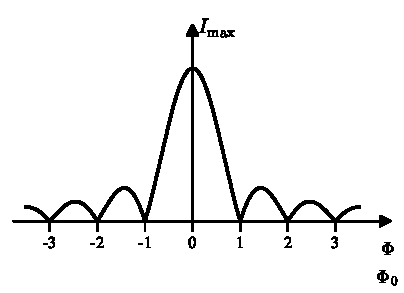
\includegraphics[width=6.5cm]{fig6-19.pdf}\\{\small 图 6.19\quad 通过约瑟夫森结的超电流最大值与磁通量之间的关系}
\end{minipage}
\end{center}

交流约瑟夫森效应：利用规范不变的相位差公式(6.10.48)还可以导出交流约瑟夫森效应.设沿z方向存在电场 $E_{z}$，根据电动力学
$E_{z}=-\dfrac{1}{c}\left(\dfrac{\partial A_{z}}{\partial t}\right)$，
矢量势 $A_{z}$ 应随时间t变化，这时对式(6.10.48)求时间导数，得到
\begin{equation}
  \frac{\partial\gamma}{\partial t}
  =-\frac{2e}{\hbar c}\int_{1}^{2}\frac{\partial A_{z}}{\partial t}\,\mathrm{d}z
  =\frac{2e}{\hbar}\int_{1}^{2}E_{z}\,\mathrm{d}z
  =\frac{2eV}{\hbar}
\end{equation}
其中V代表结区的电压.当V为常量电压 $V_{0}$ 时，$\gamma$ 是时间t的线性函数
$\gamma=\left(2eV_{0}/\hbar\right)t+\gamma_{0}$，
其中 $\gamma_{0}$ 代表1与2两块超导体间的初始相位差，因此约瑟夫森电流密度为
\begin{equation}
  j_{z}=j_{0}\sin\gamma=j_{0}\sin\left(\omega_{0}t+\gamma_{0}\right)
\end{equation}
其中
\begin{equation}
  \omega_{0}=\frac{2eV_{0}}{\hbar}
\end{equation}
上式表明，当两块超导体间存在恒定电压 $V_{0}$ 时，将产生频率为 $\omega_{0}$ 的交变电流，这时式(6.10.52)乘以隧道结的截面积LD就得到式(6.10.42)，此即著名的交流约瑟夫森效应.当外加压 $V_{0}=10\ \mu\mathrm{V}$ 时，交流约瑟夫森电流的频率为
$\omega_{0}=483.6\times10^{7}\,\mathrm{Hz}$，
恰好落在微波频率范围.人们自然会想到，如果用频率为 $\omega$ 的微波辐射照射处于直流偏压 $V_{0}$ 的约瑟夫森结将会出现反映交流约瑟夫森效应特征的新现象.事实上，约瑟夫森本人在预言交流约瑟夫森效应时就提出了这个设想，并建议以此作为验证交流约瑟夫森效应的实验手段.这时在隧道结两端的电压为
\begin{equation}
  V(t)=V_{0}+v_{0}\cos\omega t
\end{equation}
其中 $v_{0}\cos\omega t$ 是附加微波交变电压，而 $\omega$ 是微波频率，将上式代入式(6.10.51)，积分后可求出结两边超导体的电流相位差
\begin{equation}
  \gamma(t)=\frac{2e}{\hbar}V_{0}t+\gamma_{0}
  +\frac{2ev_{0}}{\hbar\omega}\sin\omega t
\end{equation}
和相应的超电流密度
\begin{equation}
  j_{\mathrm{s}}(t)=j_{0}\sin\left[\left(\frac{2e}{\hbar}V_{0}t+\gamma_{0}\right)
  +\left(\frac{2ev_{0}}{\hbar\omega}\right)\sin\omega t\right]
\end{equation}
再利用熟知的数学公式
\begin{equation*}
  \cos\left(a\sin x\right)=\sum_{m=-\infty}^{\infty}\mathrm{J}_{m}(a)\cos mx\text{，}
  \qquad
  \sin\left(a\sin x\right)=\sum_{m=-\infty}^{\infty}\mathrm{J}_{m}(a)\sin mx
\end{equation*}
又得到一个有用的公式
\begin{equation}
  \sin\left(b+a\sin x\right)
  =\sum_{m=-\infty}^{\infty}\mathrm{J}_{m}(a)\sin\left(b+mx\right)
\end{equation}
其中 $\mathrm{J}_{m}$ 代表m阶柱贝塞尔（Bessel）函数.若取 $a=\left(\dfrac{2ev_{0}}{\hbar\omega}\right)$、
$b=\left(2e/\hbar\right)V_{0}t+\gamma_{0}$ 和 $x=\omega t$，则式(6.10.56)可表示为
\begin{equation}
  j_{\mathrm{s}}(t)=j_{0}\sum_{m=-\infty}^{\infty}
  \mathrm{J}_{m}\left(\frac{2ev_{0}}{\hbar\omega}\right)
  \sin\left[\left(\frac{2e}{\hbar}V_{0}+m\omega\right)t+\gamma_{0}\right]
\end{equation}
注意在 $V_{0}$ 取任意值时，一般说来因子
$\left(\dfrac{2e}{\hbar}V_{0}t+m\omega\right)$ 不等于零，上式中所有的项都是交变电流.但是，对于某些特定的直流偏压 $V_{0}$，当满足
\begin{equation}
  2eV_{0}=n\hbar\omega
  \qquad\left(n=0,1,2,\cdots\right)
\end{equation}
时，情况却发生了变化，此时 $j_{\mathrm{s}}$ 中将出现一组零频电流项（即不随时间变化的直流项），它们可表示为
\begin{equation}
  j^{\mathrm{DC}}_{\mathrm{s}}
  =\mathrm{j}_{0}\left(-1\right)^{n}\mathrm{J}_{n}
  \left(\frac{2ev_{0}}{\hbar\omega}\right)\sin\gamma_{0}
\end{equation}
其中利用了n为正整数时柱贝塞尔函数的
$\mathrm{J}_{-n}(\varepsilon)=\left(-1\right)^{n}\mathrm{J}_{n}(\varepsilon)$
特性.上式表明，当初始相位差 $\gamma_{0}$ 从 $\left(-\pi/2\right)$ 变到 $\left(\pi/2\right)$ 时，电压
$V_{0}=\left(n\hbar\omega/2e\right)$ 保持不变，而超电流则从
$-|I_{0}\mathrm{J}_{n}\left(2ev_{0}/\hbar\omega\right)|$ 垂直地上升到
$+|I_{0}\mathrm{J}_{n}\left(2ev_{0}/\hbar\omega\right)|$，并在 $I$-$V$ 曲线上形成一个直流的台阶，表现出如图6.20所示的台阶结构.1964年夏皮洛（Shapiro）\textsuperscript{[15]}在
$\mathrm{Al-Al_{2}O_{3}-Sn}$ 结中首先观察到了这种电流增加一定幅度，而电压却维持不变的台阶，习惯上称为夏皮洛台阶.形成夏皮洛台阶的物理原因是由于在直流偏压下约瑟夫森结所产生的交变超电流被频率相同微波（或射频）场所调制，从而产生零频率的直流超电流分量.因此，在实验上观测到夏皮洛台阶就表明交流约瑟夫森效应已被证实.

\begin{center}
\begin{minipage}{7cm}
\centering
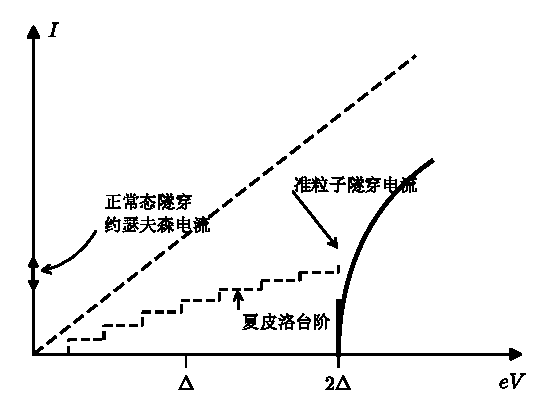
\includegraphics[width=7cm]{fig6-20.pdf}\\{\small 图 6.20\quad $I$-$V$ 曲线中夏皮洛台阶的示意图}
\end{minipage}
\end{center}

由于在第n个台阶处的电压与微波频率严格地满足
$n\omega=\left(2e/\hbar\right)V_{n}$ 关系，因此精确测定微波频率和电流阶跃处的电压可以用来精确地测定物理学中的普适常数 $\left(2e/\hbar\right)$.在20世纪60年代末期，利用交流约瑟夫森效应测出了 $\left(2e/\hbar\right)$ 的精确值，并推算出精细结构常数
$\alpha=\left(e^{2}/\hbar c\right)$，
从而解决了氢原子的超精细能级分裂的实验测量与量子电动力学理论之间的矛盾.此外，由关系式 $V_{n}=n\omega\left(\hbar/2e\right)$ 还可得知，只要选定一个台阶的号码，就可以通过测量频率 $\omega$ 而计算出台阶的电压，又由于微波频率可以精确测量到 $10^{-9}$ 甚至更高的精度，所以通过测定频率来测量电压可以达到很高的精确度.目前，利用这一方法所制成的超导电压基准已被广泛采用.

直流约瑟夫森效应的最重要应用是制作超导量子干涉仪（superconducting quantum interference devices，简称SQUID），这种仪器可用作探查或测量极其微弱的磁场.最简单的SQUID是由两个约瑟夫森结并联组成的环结构，如图6.21.为简单起见，设两个结具有相同的临界超电流 $I_{\mathrm{s}}$，外磁场垂直于环路平面，由于垂直磁场的结区面积比超导环的面积小得多，可略去透过结区的磁通，将超导环所包围的磁通量 $\Phi$ 表示为
\begin{equation}
  \Phi=\int_{S}\boldsymbol{B}\cdot\mathrm{d}\boldsymbol{S}
  =\oint\boldsymbol{A}\cdot\mathrm{d}\boldsymbol{l}
  =\int_{c}^{a}\boldsymbol{A}\cdot\mathrm{d}\boldsymbol{l}
  +\int_{b}^{d}\boldsymbol{A}\cdot\mathrm{d}\boldsymbol{l}
\end{equation}

\begin{center}
\begin{minipage}{7cm}
\centering
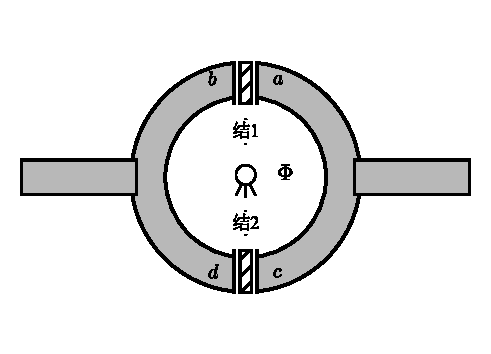
\includegraphics[width=7cm]{fig6-21.pdf}\\{\small 图 6.21\quad 双结超导干涉仪示意图}
\end{minipage}
\end{center}

而通过环的总超电流应等于通过两个结的直流约瑟夫森电流之和
\begin{equation}
  I=I_{\mathrm{J}}\left[\sin\left(\varphi_{a}-\varphi_{b}\right)
  +\sin\left(\varphi_{c}-\varphi_{d}\right)\right]
\end{equation}
其中 $I_{\mathrm{J}}$ 代表存在外磁场时单个约瑟夫森结中的最大超电流，由式(6.10.50)决定.当两个结不相干时，它们的相位差 $\left(\varphi_{a}-\varphi_{b}\right)$ 和
$\left(\varphi_{c}-\varphi_{d}\right)$ 是彼此独立的，并可以同时调节到 $\left(\pi/2\right)$，使最大的I值为 $2I_{\mathrm{J}}$，这时只有单结的衍射效应，而没有双结干涉效应.实际上a与c（或b与d）之间是超导连接，这时两个结的相位差不再是独立的，而是在 $\varphi_{a}$ 与 $\varphi_{c}$ $\left(\varphi_{b}\right.$ 与 $\left.\varphi_{d}\right)$ 之间存在着一定的约束关系，考虑到a与c是同一超导体内的两点，这两点间的相位差应满足式(6.10.46)，当超导环的横截面线度 $L\gg\lambda$（磁场的穿透深度）时，可将超导体内迈斯纳态的电流密度 $j_{\mathrm{s}}$ 取为零，这时有
\begin{equation}
  \nabla\varphi=\left(2e/\hbar c\right)\boldsymbol{A}
\end{equation}
对上式作路积分后可得
\begin{equation}
  \left.
  \begin{aligned}
    \varphi_{a}-\varphi_{c}
    &=\left(2e/\hbar c\right)\int_{c}^{a}\boldsymbol{A}\cdot\mathrm{d}\boldsymbol{l}\\
    \varphi_{b}-\varphi_{d}
    &=\left(2e/\hbar c\right)\int_{d}^{b}\boldsymbol{A}\cdot\mathrm{d}\boldsymbol{l}
  \end{aligned}\right\}
\end{equation}
从而求出结1与结2相位差之间的约束关系
\begin{equation}
\begin{aligned}
  \left(\varphi_{a}-\varphi_{b}\right)-\left(\varphi_{c}-\varphi_{d}\right)
  &=\left(\varphi_{a}-\varphi_{c}\right)+\left(\varphi_{d}-\varphi_{b}\right)\\
  &=\left(2e/\hbar c\right)\left(\int_{c}^{a}+\int_{b}^{d}\right)
  \boldsymbol{A}\cdot\mathrm{d}\boldsymbol{l}\\
  &=\left(2e/\hbar c\right)\Phi=2\pi\left(\Phi/\Phi_{0}\right)
\end{aligned}
\end{equation}
其中利用了式(6.10.61)和磁通量子 $\Phi_{0}=\left(\pi\hbar c/e\right)$.这时最好将式(6.10.62)变换为正、余弦函数之乘积，并利用约束关系式(6.10.65)求出
\begin{equation}
\begin{aligned}
  I&=2I_{\mathrm{J}}\cos\left[\frac{1}{2}
  \left(\varphi_{a}-\varphi_{c}+\varphi_{d}-\varphi_{b}\right)\right]
  \sin\left[\frac{1}{2}
  \left(\varphi_{a}+\varphi_{c}-\varphi_{d}-\varphi_{b}\right)\right]\\
  &=2I_{\mathrm{J}}\cos\left(\pi\Phi/\Phi_{0}\right)\sin\gamma_{0}
\end{aligned}
\end{equation}
其中
\begin{equation*}
  \gamma_{0}\equiv\frac{1}{2}
  \left(\varphi_{a}+\varphi_{c}-\varphi_{d}-\varphi_{b}\right)
  =\frac{1}{2}\left[\left(\varphi_{a}-\varphi_{b}\right)
  +\left(\varphi_{c}-\varphi_{d}\right)\right]
\end{equation*}
代表两个结的相位差之和，它可以任意调节，当 $\gamma_{0}=\pi/2$ 时，双结系统的超电流最大值为
\begin{equation}
  I_{\max}=2I_{\mathrm{J}}\left|\cos\left(\pi\Phi/\Phi_{0}\right)\right|
\end{equation}

\begin{center}
\begin{minipage}{7cm}
\centering
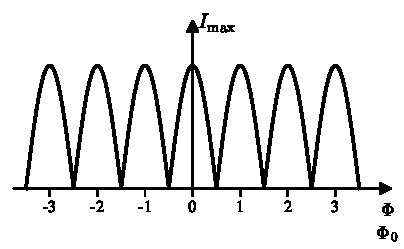
\includegraphics[width=7cm]{fig6-22.pdf}\\{\small 图 6.22\quad 双结超导环的干涉效应}
\end{minipage}
\end{center}

图6.22是以 $I_{\mathrm{J}}$ 为单位、$I_{\max}$ 随 $\left(\pi\Phi/\Phi_{0}\right)$ 的变化曲线.显然，当环路所包含的 $\Phi$ 为 $\Phi_{0}$ 的整数倍时，给出 $I_{\max}$ 之极大值，而当 $\left(\Phi/\Phi_{0}\right)$ 为半整数时 $I_{\max}$ 降为零，它至少可以区别半个磁通量子
$\Phi_{0}=2\times10^{-7}\,\mathrm{Gs\cdot cm^{2}}$ 的变化，这就是双结干涉效应.由于超导环路所包围的面积S是可以人为控制的，人们只需制作面积的数量级为 $1\ \mathrm{cm^{2}}$ 的双结超导环，就可以探测到 $10^{-7}\,\mathrm{Gs}$ 的磁场变化.因此，双结干涉效应可用于制作高精度的磁场测量仪——磁强计.

在以上的讨论中，我们还没有考虑单结衍射效应对双结干涉效应的影响.若再将式(6.10.67)中的 $I_{\mathrm{J}}$ 用外磁场中的单结衍射公式(6.10.50)代入，则求得包括了干涉与衍射效应的双结系统的超电流最大值满足
\begin{equation}
  I_{\max}=2I_{0}\left|\frac{\sin\left(\pi\Phi_{\mathrm{J}}/\Phi_{0}\right)}
  {\left(\pi\Phi_{\mathrm{J}}/\Phi_{0}\right)}\right|
  \left|\cos\left(\pi\Phi/\Phi_{0}\right)\right|
\end{equation}
其中 $\Phi_{\mathrm{J}}$ 是结区穿透范围内的磁通量，由于超导环路所包围的面积S远远大于结区被磁场穿透的面积，在上式中，$\Phi_{\mathrm{J}}\ll\Phi$（穿过环路的总磁通量），这时上式中因子
$\left|\cos\left(\pi\Phi/\Phi_{0}\right)\right|$ 导致 $I_{\max}$ 随外磁场作小周期的快速振荡，而来自结衍射效应的
$\left|\sin\left(\pi\Phi_{\mathrm{J}}/\Phi_{0}\right)
/\left(\pi\Phi_{\mathrm{J}}/\Phi_{0}\right)\right|$
因子则随磁场作较长周期的衰减振荡，从而对小周期振荡的干涉效应起着调制作用.理论与实验结果都表明双结系统的 $I_{\max}$-$B$ 曲线如图6.23所示，它显示出受到衍射调制的干涉图样.最后，我们还要指出，仅仅根据 $I_{\max}$ 从极大变为极小（即一个干涉条件），只能测定出数量级为一个磁通量子 $\Phi_{0}$ 的磁场 $\left(10^{-7}\,\mathrm{Gs}\right)$，而当 $\Phi=\Phi_{0}$ 时，必然有 $\Phi_{\mathrm{J}}\ll\Phi_{0}$，这时式(6.10.68)退化为式(6.10.67).因此，作微小磁场测量时，主要是利用干涉效应，即式(6.10.67).目前在双结干涉效应基础上人们已制造出直流SQUID，其中利用补偿磁通（或抵消磁场）方法已能读出 $10^{-4}\Phi_{0}$ 的微小磁通变化，相当于能分辨出 $10^{-11}\,\mathrm{Gs}$ 微弱磁场变化，详细讨论可参阅文献\textsuperscript{[16]}.

\begin{center}
\begin{minipage}{7cm}
\centering
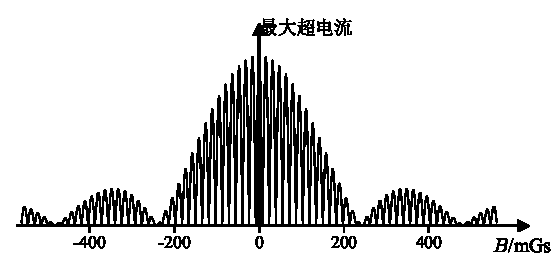
\includegraphics[width=7cm]{fig6-23.pdf}\\{\small 图 6.23\quad 双结SQUID的衍射调制干涉图样}
\end{minipage}
\end{center}

\begin{canKao}
\begin{enumerate}[label={[\arabic*]}, leftmargin=2.2em, itemsep=0pt]
\item Cooper L N. Phys Rev, 1956, 104: 1189
\item Bardeen J, Cooper L N, Schrieffer J R. Phys Rev, 1957, 103: 1175
\item Mahen G D. Many-particle Physics. New York: Plenum Press, 1981. Chap 7
\item De Gennes P G. Superconductivity of Metals and Alloys. New York: Benjamin, 1966. Chap 8
\item Schrieffer J R. Theory of Superconductivity. New York: Benjamin, 1964
\item Giaever L. Phys Rev Lett, 1960, 5: 147, 464
\item 管惟炎等. 超导电性. 北京: 科学出版社，1981. 第6章
\item Fetter A L, Walecka J D. Quantum Theory of Many-particles System. New York: Mc-Graw-Hill, 1971. Chap 13
\item Ginzburg V L, Landau L D. Zh Eksper Teor Fis, 1950, 24: 1064
\item Saint-James D et al. Type Ⅱ Superconductors. London: Pergamon Press, 1969
\item Deaver B S, Fairbank W M. Phys Rev Lett, 1961, 7: 43
\item Abrikosov A A. Zh Eksper Teor Fis, 1957, 32: 1442
\item Josephson B D. Phys Lett, 1960, 1: 251; Adv Phys, 1965, 14: 419
\item Anderson P W, Rowell J M. Phys Rev Lett, 1963, 10: 230
\item Shapiro S. Phys Rev Lett, 1963, 11: 80
\item 陈式刚等. 高温超导研究. 四川教育出版社，1991.6
\end{enumerate}
\end{canKao}

% ============================================================
%  第七章 氧化物高温超导体和各向异性超导电性（§1–§8 + 章末参考文献）
%  底本：高等教育出版社《固体理论》第二版；原书印刷页 229–285
%  （PDF 页 = 印刷页 + 20）
%  公式编号自检：§3 (7.3.1)–(7.3.4)；§4 (7.4.1)–(7.4.45)
%    （(7.4.13a/b)、(7.4.23a/b)、(7.4.30a/b)、(7.4.32a/b)、
%    (7.4.33a/b)、(7.4.34a/b) 为原书自带二级编号，用 subequations
%    环境照录，与 ch04/ch06 体例一致）；§5 (7.5.1)–(7.5.7)；
%    §6 (7.6.1)–(7.6.19)；§7 (7.7.1)–(7.7.14)。
%    全章自动编号 89 个，各节均无缺号。
%
%  任务单所列 6 处"缺号"逐条对照原书页面判定（均非原书跳号）：
%    (7.4.1)  原书 p252 在号（OCR 乱码）；
%    (7.5.2)  原书 p261 在号（OCR tag 误作逗号 7.5,2）；
%    (7.5.4)  原书 p261 在号（OCR tag 本在）；
%    (7.5.6)  原书 p263 在号（OCR tag 残缺作 (.6)，已按页面补排）；
%    (7.6.9)  原书 p267 在号（OCR 乱码，已按页面补排）；
%    (7.7.12) 原书 p276 在号（OCR tag 断作 (7.7.+12）。
%  另：OCR 中 \tag{C.7} 为所引附录 C 公式编号（原书 p256 照排
%    (C.7)），用 \tag 照录，不占章内公式计数。
%
%  已修正的 OCR/原书错误（除全角句点转"."、删 ~ 间隔符、收紧
%  \mathrm{d}、拆开行内公式与中文等常规项外）：
%  1. 表 7.1 OCR 串行，按 p230 原表逐格复原（Hg-1223 之 H_c
%     值原书即空缺）；O_{10+1}→O_{10+x}。
%  2. §1 HoMo_6S_6（OCR 误作 H_0M_06S_6、ΔT_c=2ΔK）按 p230 复原；
%     "在加高压条件下 T_c 一般仍限于 10 K 之内"语序按 p230 复原；
%     "载流子流度"→"载流子浓度"、"确实出人意料"等粘连按 p231 复原；
%     La-Ba-Cu-O、La_2-xM_xCuO_4、Nd_2-xCe_xCuO_4 等化学式按
%     p231–232 复原；"superrcon-ducting"→superconducting。
%  3. §1 "交换反铁磁自旋涨落"原书漏"磁"字（p230），按文意补。
%  4. §2 "这些结构均具有正交对称性"OCR"匀"→均（p235）；"例如在
%     La-214 与 Bi-2201 中"OCR 串行按 p235 复原；"引人"→引入
%     （p238）；图 7.2(b) YBa_2Cu_3O_{6+x}（OCR Cu_8）；"超导相干
%     长度"OCR"相于"→相干（p245）。
%  5. §2.1 (ii) 结构单元图示与 (iii) La-214 掺杂表格 OCR 乱码，
%     按 p236–237 原书复原（La^{3+}_{1-x/2}(Sr^{2+})_{x/2}O^{2-}_4
%     等按原书照排）。
%  6. (7.3.1) arctan(k_y/k_x) OCR 多余 \mid 已删（p243 无绝对值）。
%  7. §3.1 "两个载流配对"原书如此（p241），照录。
%  8. §3.2 "扫描述磁强计""半整的量子磁通""首先制了成全由"等
%     原书排印如此（p244），照录。
%  9. 表 7.2 按 p245 原表复原；Nb 行 λ、ξ 为合并格。
% 10. (7.4.10) 第二等式积分下标 FS（OCR 误作 F^3，p253）；
%     (7.4.12) 第二行 Y_{l'm'} 补撇；(7.4.13b) 积分内 ψ_l(k') 与
%     积分限 ε_{k'} 按 p253 复原（OCR 误作 φ、ε_k）。
% 11. (7.4.15) 按 p253 复原：∫_0^{ħω_0} dε/(2ε-E)（OCR 乱码）。
% 12. (7.4.23b) 等号后原书衍一竖线"|"（p256 排印残迹），已删。
% 13. (7.4.26) OCR 之 \hat\theta、\hat\delta 按 p256 复原为 δ；
%     末尾逗号已删。
% 14. 表 7.5 按 p254 复原（单重态自旋波函数 (↑↓-↓↑)/√2）。
% 15. (7.4.34a)、(7.4.39)、(7.4.42) OCR 严重乱码按 p258、260 复原。
% 16. §5 (7.5.3)(7.5.4)(7.5.5) 按 p261 复原（Σ 积分域、cases）；
%     (7.5.6) 中间情形 (1/i)∫_{-1}^{1}dx/√(x^2-(ω/Δ_0)^2) 按 p263
%     复原；(7.5.7) cases 按 p263 复原。
% 17. §5.2 "重费密子超导体具有奇异特性"OCR 漏"子"（p264）；
%     "表中的低温比热容……"固体物理公式按 p264 复原。
% 18. 表 7.6 按 p264 原表逐格复原（c_es 行 ~T^{2.8}、~T^{2.86} 等；
%     T_{1s}^{-1} 行 ~T^3(^{63}Cu)、~T^3(^{9}Be)、~T^3(^{195}Pt)；
%     Δλ 行 d 波极向态 {T(纯); T^2(含杂)}）。
% 19. §5.2"仔细分析表7.5中"与 §6.2"表7.5中所用的固体物理学公式"
%     两处原书引号有误：所指均为表 7.6 及其下注公式，按 p264/266
%     更正为表 7.6。
% 20. (7.6.2) 按 p265 复原（OCR 乱码）；(7.6.9) 按 p267 复原；
%     §6.3 二维能隙方程（未编号）及零温能隙推导诸式（未编号）
%     按 p268 复原；(7.6.14) OCR \bigcup(0)→Δ_0(0)、Ψ_d→V_d。
% 21. (7.7.13) OCR 乱码按 p277 复原；"约飞(Ioffe)判据"按 p272
%     复原；图 7.14 图注原书"核自系统"漏"旋"字（p277），补为
%     "核自旋系统"。
% 22. §7.1 ρ_0 句"ρ_0 为将 ρ_ab(T) 的线性关系外延到绝对零度时的
%     插值"按 p271 复原。
% 23. §8.2 "研究组[35]"补全上标括号；Δ_BCS(T_c)=0 按 p283 复原；
%     (7.6.1) 中 φ=arctan(k_y/k_x)（OCR 衍符已清）。
% 24. §3.4 "但在解释同位素效应时却是不可忽略的"OCR 漏"可"
%     （p250），按原书补。
%  遗留问题：
%  · 图 7.1–7.17 均为占位图（figures/fig7-N.pdf），重绘代理负责；
%    图 7.2、7.6、7.7、7.16 原书为多图（(a)/(b) 或 (a)/(b)/(c)）
%    结构，图注按原书补子图说明。
%  · 原书 p244 "扫描述磁强计""半整的量子磁通"、p244 "首先制了成"
%    、p241 "两个载流配对"、p250 "弱杂的Y-123"、p281 "使态k态的
%    态密度"等均系原书排印如此，未改动。
%  · 原书用字"费密"照录；仅 p239 一处"费米液体"原书即作"费米"，
%    照录未改。
% ============================================================
\chapter{氧化物高温超导体和各向异性超导电性}

本章主要介绍铜氧化合物高温超导体的基本属性.我们将首先对提高超导转变温度的历史进程作一个简单的回顾（§1），然后介绍高温超导体的结构与相图（§2）以及超导态（§3）的共同特征.为了理解高温超导体的超导态与BCS超导态的不同之处，我们将先介绍各向异性配对的超导理论（§4、§5），然后用此理论来解释高温超导体的异常超导特性（§6）.最后，介绍高温超导体正常态的反常特性（§7）以及在弱掺杂区发现正常态能隙所提出的物理问题（§8）.

\section{\texorpdfstring{高$T_{\mathrm{c}}$——超导电性研究的重大突破}{高Tc——超导电性研究的重大突破}}

自从1911年昂内斯（Kammerlingh Onnes）在4.2 K发现 $\mathrm{Hg}$ 的超导电性以来，提高超导转变温度 $T_{\mathrm{c}}$ 就已经成为超导电性研究的主要目标之一，经过许多科学家的长期探索，人们已发现了千余种常规超导体，包括元素超导体及合金与化合物超导体.在元素周期表中，已经发现具有超导电性的元素超过了50种，其中在常压室温下为典型半导体的 $\mathrm{Ge}$ 和 $\mathrm{Si}$，通过加高压（约200 kbar）使之金属化以后，也可进入超导态，并测得 $T_{\mathrm{c}}=6.7$ K（Si）和5.3 K（Ge），其它的在高压下才发现具有超导电性的元素还有P、As、Se、Y、Sb、Te、Cs、Ba、Bi、Ce和U等.尽管如此，在元素超导体中测得的最高转变温度是 $T_{\mathrm{c}}=9.3$ K（Nb），仍处于液He温区，而且元素超导体的临界磁场 $H_{\mathrm{c}}$ 一般都很低，无应用价值，如表7.1所示\textsuperscript{[1]}.

为了获得具有实用价值的超导材料，从20世纪60年代起人们又发现配制超导合金与化合物可进一步提高 $T_{\mathrm{c}}$ 和 $H_{\mathrm{c}}$，并成功地用 Nb-Ti 合金制成了可在4.2 K工作的10 T的超导磁体.只是数十年来 $T_{\mathrm{c}}$ 的提高十分缓慢，直至1973年才在 $\mathrm{Nb}_{3}\mathrm{Ge}$ 超导薄膜中观测到 $T_{\mathrm{c}}=27.3$ K，使超导进入液氢温区，对应用并未带来方便.因此，寻找更高转变温度的超导体仍是科学家梦寐以求的目标.

表7.1\quad 超导转变温度和临界磁场提高的编年表

\begin{center}\small
\begin{tabular}{clccc}
\hline
 & 超导体 & $T_{\mathrm{c}}$/K & $H_{\mathrm{c}}$/T & 观测年代\\
\hline
常规超导体 & $\mathrm{Hg}$ & 4.2 & 0.04 & 1911\\
 & $\mathrm{Pb}$ & 7.2 & 0.08 & 1913\\
 & $\mathrm{Nb}$ & 9.3 & 0.20 & 1930\\
 & Nb-Ti合金 & 10.0 & 14 & 1954\\
 & $\mathrm{V}_{3}\mathrm{Si}$ & 17.1 & 21 & 1954\\
 & $\mathrm{Nb}_{3}\mathrm{Sn}$ & 18.1 & 24 & 1954\\
 & $\mathrm{Nb}_{3}\mathrm{Ge}$ & 27.3 & 38 & 1973\\
\hline
高温超导体 & $\mathrm{La}_{2-x}\mathrm{Sr}_{x}\mathrm{CuO}_{4}$（La-214） & 40 & 40 & 1986\\
 & $\mathrm{YBa}_{2}\mathrm{Cu}_{3}\mathrm{O}_{6+x}$（Y-123） & 92 & $>$100 & 1987\\
 & $\mathrm{Bi}_{2}\mathrm{Sr}_{2}\mathrm{Ca}_{2}\mathrm{Cu}_{3}\mathrm{O}_{10+x}$（Bi-2223） & 110 & $>$120 & 1988\\
 & $\mathrm{Tl}_{2}\mathrm{Ba}_{2}\mathrm{Ca}_{2}\mathrm{Cu}_{3}\mathrm{O}_{10+x}$（Tl-2223） & 125 & $>$130 & 1988\\
 & $\mathrm{HgBa}_{2}\mathrm{Ca}_{2}\mathrm{Cu}_{3}\mathrm{O}_{8+x}$（Hg-1223） & 133（$>$160加压） & & 1993\\
\hline
\end{tabular}
\end{center}

为了改写常规超导体中 $T_{\mathrm{c}}=27.3$ K的最高纪录，1973年以后科学家们想方设法进行开拓.他们首先在稀土三元化合物 $\mathrm{ErRh}_{4}\mathrm{B}_{4}$（$T_{\mathrm{c}}=8.7$ K）及 $\mathrm{HoMo}_{6}\mathrm{S}_{6}$（$T_{\mathrm{c}}=2$ K）中发现了铁磁超导体，又在 $\mathrm{GdMo}_{6}\mathrm{S}_{8}$（$T_{\mathrm{c}}=1.4$ K，$T_{\mathrm{N}}=0.95$ K）与 $\mathrm{TbMo}_{6}\mathrm{S}_{8}$（$T_{\mathrm{c}}=1.65$ K，$T_{\mathrm{N}}=1$ K）等材料中发现了反铁磁超导体，并展开了磁与超导相互竞争与共存的研究.继之，又在低维（准一维与准二维）的有机化合物中发现了超导电性，这类有机超导体的载流子浓度很低，还存在着磁性与超导电性之间的相互竞争现象，是探索超导新机制的一个重要领域，但其转变温度不高，在加高压条件下 $T_{\mathrm{c}}$ 一般仍限于10 K之内.1979年以后，人们又在含稀土与锕系元素的金属间化合物中找到了新的一类超导体：$\mathrm{CeCu}_{2}\mathrm{Si}_{2}$（$T_{\mathrm{c}}=0.5$ K）、$\mathrm{UBe}_{13}$（$T_{\mathrm{c}}\approx1$ K）及 $\mathrm{UPt}_{3}$（$T_{\mathrm{c}}\approx0.54$ K），其超导电性与 Ce 及 U 中具有很高有效质量（$m^{*}\geqslant200\,m_{\mathrm{e}}$）的4f 及 5f 电子有关，故称为重费密子超导体（HFS）.重费密子超导体属于强关联电子体系（同一格点上的4f或5f电子间存在强库仑关联），具有和BCS超导体明显不同的超导态特性，最突出的一点就是重费密子超导体是各向异性超导体，其费密面上的能隙函数具有零点或零线，属于下面将讨论的d波或p波配对情形，而且产生配对的吸引并非电子-声子相互作用，极有可能是重费密子间交换反铁磁自旋涨落（一类玻色型元激发）所形成的.在20世纪80年代初期，重费密子超导体的这些奇异特征曾吸引了物理学家探索超导新机制的浓厚兴趣，只可惜重费密子超导体的转变温度太低，谈不上应用价值.

值得一提的是氧化物超导体的研究，早在1964年，人们就在具有钙钛矿结构（$\mathrm{ABO}_{3}$）的氧化物 $\mathrm{SrTiO}_{3}$ 中发现了超导电性，其 $T_{\mathrm{c}}$ 很低，仅为0.4 K，这并不奇怪，因为在这类氧化物中载流子浓度很低（$n<10^{21}\,\mathrm{cm}^{-3}$），对应的费密面上态密度 g(0) 自然也很小，根据BCS的 $T_{\mathrm{c}}$ 公式(6.5.10)，其转变温度仍然很低.但是经过十年多的研究，人们发现在这类 $\mathrm{ABO}_{3}$ 结构的掺杂系统（如 $\mathrm{BaPb}_{1-x}\mathrm{Bi}_{x}\mathrm{O}_{3}$）中，当 x 在0.25～0.3之间时（接近金属-绝缘体转变点时），尽管其载流子浓度仍为 $10^{21}\,\mathrm{cm}^{-3}$ 数量级，但 $T_{\mathrm{c}}$ 却可以上升到13 K，令人费解.另一方面从制作超导材料的经验可知，一般要获得 $T_{\mathrm{c}}>10$ K 的化合物，都需要含有Nb或V等过渡族元素，在不含这类过渡金属元素的氧化物中也能获得较高的 $T_{\mathrm{c}}$ 值，确实出人意料.理论分析也表明其超导配对机制不能简单地用BCS的电子-声子互作用模型说明，而很可能来源于电子-电子相互作用.这时，包括穆勒（Müller）与伯诺兹（Bednorz）在内的一批科学家已经意识到研究掺杂 $\mathrm{ABO}_{3}$ 型氧化物材料有可能导致新的超导机制和更高 $T_{\mathrm{c}}$ 超导体的发现.1983年，穆勒提出了开展氧化物超导电性研究的计划，并在具有研究 $\mathrm{ABO}_{3}$ 型绝缘化合物传统的苏黎世IBM实验室与伯诺兹进行合作，在经历了研究 La-Ni-O 系统的失败之后，他们于1985年转向对铜氧化合物进行研究.1986年铜氧化合物高温超导体的发现也正是在这种背景下产生的.应该说，它是学科发展和人们长期努力的必然结果.

在1986年以前的13年中，超导电性的研究虽然发现了不少新领域，令人开阔了眼界，但令人失望的是超导转变温度的最高纪录 $T_{\mathrm{c}}=27.3$ K（1973年）始终未能改写，这是提高 $T_{\mathrm{c}}$ 的一个低潮期.在此期间不少理论研究者甚至声称常规的BCS超导体不可能突破 $T_{\mathrm{c}}=30$ K 的大关，但是，就在1986年4月，伯诺兹和穆勒\textsuperscript{[2]}公布了他们在 La-Ba-Cu-O 化合物中观察到起始超导转变温度为35 K的结果.这一出人意料的发现开创了 $T_{\mathrm{c}}$ 的新纪录，导致了在全世界范围内掀起探索高温超导体 $T_{\mathrm{c}}$ 的热潮，伯诺兹与穆勒的结果很快被同行所证实和加以改进，并在掺入二价金属 M（Ba、Sr等）的 $\mathrm{La}_{2-x}\mathrm{M}_{x}\mathrm{CuO}_{4}$ 化合物体系中获得了 $T_{\mathrm{c}}$ 高于40 K的超导转变温度.为简单起见，人们将这类材料记为La-214.

1987年2月，距伯诺兹与穆勒的论文发表还不到一年，美国的朱经武研究组\textsuperscript{[3]}和我国的赵忠贤研究组\textsuperscript{[4]}先后独立地在 $\mathrm{YBa}_{2}\mathrm{Cu}_{3}\mathrm{O}_{7-y}$（后简称Y-123）化合物中发现了 $T_{\mathrm{c}}\geqslant90$ K 的氧化物高温超导体，首次使超导研究进入了液氮温区.1988年初，人们又发现了另外两组具有更高 $T_{\mathrm{c}}$ 的铜氧化合物超导体：$\mathrm{Bi}_{2}\mathrm{Sr}_{2}\mathrm{Ca}_{2}\mathrm{Cu}_{3}\mathrm{O}_{10+x}$（Bi-2223），其 $T_{\mathrm{c}}=110$ K\textsuperscript{[5]}，和 $\mathrm{Tl}_{2}\mathrm{Ba}_{2}\mathrm{Ca}_{2}\mathrm{Cu}_{3}\mathrm{O}_{10}$（Tl-2223）\textsuperscript{[6]}，其超导转变温度高达 $T_{\mathrm{c}}=125$ K\textsuperscript{[6]}.以上新发现的氧化物高温超导体都是空穴掺杂型的铜氧化合物，其正常导电载流子是空穴，可称为空穴型高温超导体.1989年日本学者\textsuperscript{[7]}在Nd基氧化物中用 $\mathrm{Ce}^{4+}$ 离子取代 $\mathrm{Nd}^{3+}$ 离子，获得了第一例电子型氧化物超导体 $\mathrm{Nd}_{2-x}\mathrm{Ce}_{x}\mathrm{CuO}_{4}$（$T_{\mathrm{c}}\approx20$ K）.

\begin{center}
\begin{minipage}{7cm}
\centering
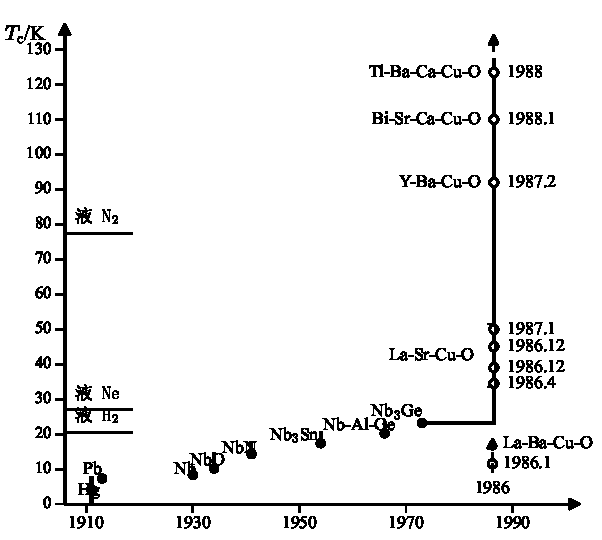
\includegraphics[width=7cm]{fig7-1.pdf}\\{\small 图 7.1\quad 超导转变温度提高的历史记录}
\end{minipage}
\end{center}

图7.1是超导转变温度提高的历史记录.显然，与1986年以前相比较，自从伯诺兹与穆勒新发现的铜氧化合物问世以来，超导转变温度屡破纪录，在不到两年的时间内 $T_{\mathrm{c}}$ 已提高了4～5倍，进入了便于工作的液氮温区，其临界磁场也很高（见表7.1），为超导电性的研究和应用开辟了一个新时期.因此，伯诺兹与穆勒在1986年的发现应当认为是超导电性研究的一个历史性的突破.正由于其贡献巨大，他们在一年之后就获得了1987年诺贝尔物理学奖.

迄今公认的最高超导转变温度也是朱经武研究组\textsuperscript{[8]}在 $\mathrm{HgBa}_{2}\mathrm{Ca}_{2}\mathrm{Cu}_{3}\mathrm{O}_{8+x}$（Hg-1223）化合物中测得的，其 $T_{\mathrm{c}}=133$ K，加压力甚至可使 $T_{\mathrm{c}}$ 提升到160 K以上.还应当指出，从1986年至今国内外还有很多更高 $T_{\mathrm{c}}$ 包括接近室温的报道，但可惜现象不稳定，样品难于重复或甚至不能重复，被朱经武教授戏称为“不明超导体”（unidentified superconducting objects，USO）\textsuperscript{[9]}.

值得一提的是，由于铜氧化合物高温超导体的 $T_{\mathrm{c}}$ 不断提高，反过来又启发和促进了常规超导体的研究.人们在 $\mathrm{C}_{60}$ 所组成的晶体中掺入足量的碱金属A（Cs、Rb等）使其金属化后，在 $\mathrm{A}_{3}\mathrm{C}_{60}$ 化合物中观测到转变温度 $T_{\mathrm{c}}$ 超过30 K的块体超导电性，属于电声子机制的BCS超导体，其中 $\mathrm{Cs}_{x}\mathrm{Rb}_{y}\mathrm{C}_{60}$ 的 $T_{\mathrm{c}}=33$ K（1991），而加压后的 $\mathrm{Cs}_{3}\mathrm{C}_{60}$（1995）$T_{\mathrm{c}}$ 可达到40 K\textsuperscript{[10]}.2000年美国巴特洛格（Batlogg）研究组在 $\mathrm{C}_{60}$ 晶体表面生长氧化层，设计了 $\mathrm{C}_{60}$ 的场效应三极管，通过调节系统的门电压可分别在 $\mathrm{C}_{60}$ 表层诱生电子或空穴，从而构成了一种载流子浓度可从电子型连续调节到空穴型的“掺杂”（不是化学掺杂，而是表面注入电子或空穴）$\mathrm{C}_{60}$ 金属系统，并发现当每个 $\mathrm{C}_{60}$ 中注入3～3.5个空穴时最高的 $T_{\mathrm{c}}$ 可达到52 K，而表层注入电子时最高 $T_{\mathrm{c}}$ 只有10 K.人们认为这是由于电子注入 $\mathrm{C}_{60}$ 的导带，空穴注入价带，而价带的能带电子态密度远远高于导带，相应的价带电声子互作用更强，导致空穴型 $\mathrm{C}_{60}$ 的 $T_{\mathrm{c}}$ 更高，但应注意在这里超导配对发生在 $\mathrm{C}_{60}$ 晶体的表面层，属于准二维系统的电声子机制超导电性（见文献\textsuperscript{[11]}中 Nature 杂志）.巴特洛格研究组在 $\mathrm{C}_{60}$ 分子间插入 $\mathrm{CHBr}_{3}$ 组成 $\mathrm{C}_{60}/\mathrm{CHBr}_{3}$ 的复合晶格，可使晶格常数从纯 $\mathrm{C}_{60}$ 的1.415 nm扩大为1.445 nm，随着晶格常数的增大，$\mathrm{C}_{60}$ 间载流子的近邻跃迁将减小，从而使能带变窄和态密度增加.根据最近的报道，他们发现当采用扩大的晶格 $\mathrm{C}_{60}/\mathrm{CHBr}_{3}$ 表面层做场效应三极管时，超导转变温度可提升到 $T_{\mathrm{c}}=117$ K，并声称如果 $\mathrm{C}_{60}$ 中再掺入适量的碱金属，$T_{\mathrm{c}}$ 还可以进一步升高（见文献\textsuperscript{[11]}中 Science 杂志），这是一个令人振奋的信息.另一个引人注目的进展是，2001年初在金属间化合物 $\mathrm{MgB}_{2}$\textsuperscript{[12]}中又发现了 $T_{\mathrm{c}}=39$ K 的块体超导电性，并已证实是电声子机制的常规超导体，它比同类二元金属间化合物 $\mathrm{Nb}_{3}\mathrm{Ge}$ 的 $T_{\mathrm{c}}$ 提高了近12 K，若进行掺杂还可以使 $\mathrm{MgB}_{2}$ 系统的 $T_{\mathrm{c}}$ 进一步提高.$\mathrm{C}_{60}$ 系列和 $\mathrm{MgB}_{2}$ 的发现突破了常规超导体的 $T_{\mathrm{c}}$ 一般不超过30 K的传统信念，引起了人们的极大兴趣，已成为当前超导电性研究的热点问题.

\section{结构与相图的共同特征}

\subsection*{1. 存在$\mathrm{CuO}_{2}$导电层——铜氧化合物结构的共同特征}

利用衍射技术可以确定新发现的铜氧化合物高温超导体的晶体结构.图7.2是两种典型氧化物超导体的结构示意，其中图(a)与图(b)分别代表 $\mathrm{La}_{2-x}\mathrm{Sr}_{x}\mathrm{CuO}_{4}$（La-214）和 $\mathrm{YBa}_{2}\mathrm{Cu}_{3}\mathrm{O}_{6+x}$（Y-123）的结构.图7.3为Bi系化合物（包括 Bi-2201，Bi-2212 和 Bi-2223）的结构.

\begin{center}
\begin{minipage}{6.5cm}
\centering
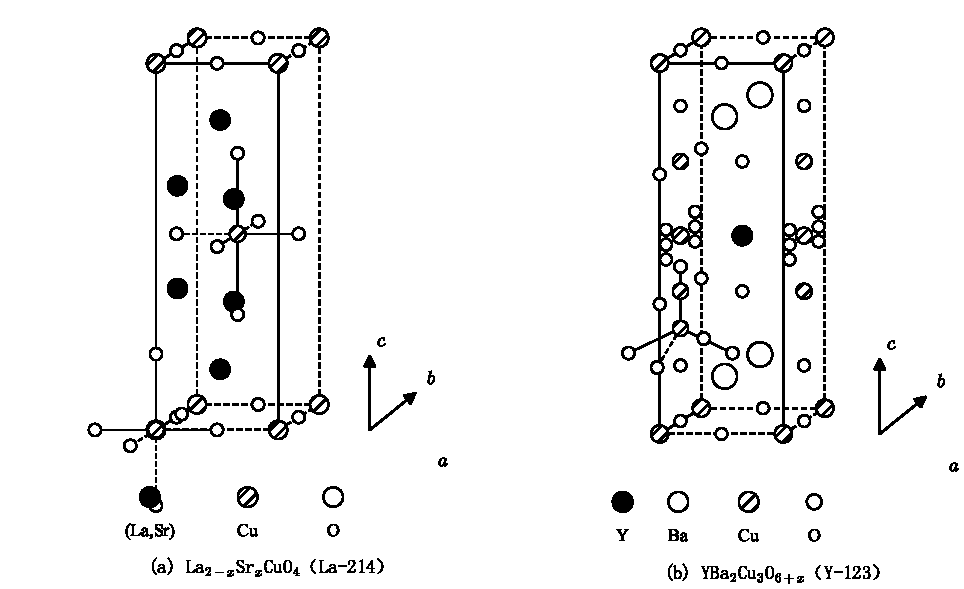
\includegraphics[width=6.5cm]{fig7-2.pdf}\\[0.3em]
{\small (a) $\mathrm{La}_{2-x}\mathrm{Sr}_{x}\mathrm{CuO}_{4}$（La-214）\qquad\qquad (b) $\mathrm{YBa}_{2}\mathrm{Cu}_{3}\mathrm{O}_{6+x}$（Y-123）}\\[0.2em]
{\small 图 7.2\quad 两种典型的氧化物高温超导体结构}
\end{minipage}
\end{center}

这些结构均具有正交对称性，其c轴方向的晶格常数大于a和b方向，是 $c>b\approx a$ 的近四方结构，它们基本上属于钙钛矿结构的变型.值得注意的是，在这些结构中均含有 $\mathrm{CuO}_{2}$ 平面层.例如在 La-214 与 Bi-2201 中只含一个 $\mathrm{CuO}_{2}$ 平面层，在 Y-123 和 Bi-2212 中含有两个 $\mathrm{CuO}_{2}$ 层，而在 Bi-2223 中则含3层，具有 $T_{\mathrm{c}}=125$ K 的 Tl-2223 和 $T_{\mathrm{c}}=133$ K 的 Hg-1223 结构也含有3层 $\mathrm{CuO}_{2}$ 平面.

\begin{center}
\begin{minipage}{6.5cm}
\centering
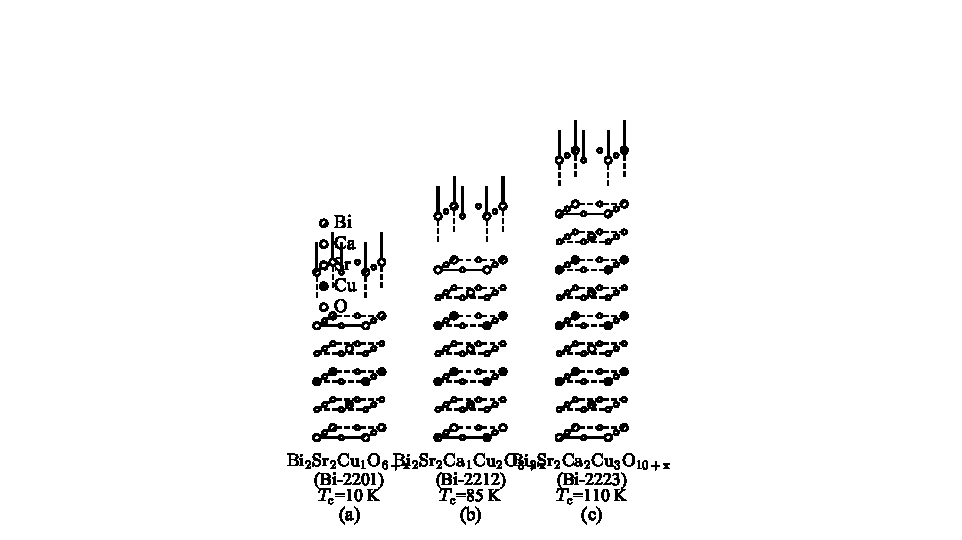
\includegraphics[width=6.5cm]{fig7-3.pdf}\\{\small 图 7.3\quad Bi系氧化物超导体的结构}
\end{minipage}
\end{center}

大量实验证据表明，这些氧化物高温超导体均具有平面导电特性，并且载流子运动主要是在 $\mathrm{CuO}_{2}$ 平面之中.能带计算也证实，系统的能带结构在费密面附近基本上不随 $k_{z}$（即垂直于 $\mathrm{CuO}_{2}$ 层方向波矢）变化，具有明显的二维特征，而且主要是来自 $\mathrm{CuO}_{2}$ 层中的电子能带贡献.另外，$\mathrm{CuO}_{2}$ 层内的 Cu 与 O 的键距也明显小于在c方向的键距，可将晶体看作为层状化合物，其中的 $\mathrm{CuO}_{2}$ 层可近似看作二维正方晶格.人们对于 $\mathrm{CuO}_{2}$ 层的作用进行了深入和集中的研究，获得了如下的主要结论：

(i) $\mathrm{CuO}_{2}$ 层对超导电性的产生起主要作用，这些层是铜氧化合物中的主要导电层，可称为导电单元.在这些化合物中的其它部分可以简单地看成是另一个结构单元，其主要作用是为导电单元（$\mathrm{CuO}_{2}$ 面或 $\mathrm{CuO}_{2}$ 面群）提供载流子，又可称为电荷库单元或简称电荷库（charge reservoir）.例如在 $\mathrm{La}_{2-x}\mathrm{Sr}_{x}\mathrm{CuO}_{4}$ 中，隔开相邻 $\mathrm{CuO}_{2}$ 导电层的两个（La，Sr）-O 层称为 La-214 的电荷库.又如在 $\mathrm{YBa}_{2}\mathrm{Cu}_{3}\mathrm{O}_{6+x}$ 结构中，导电单元由两层 $\mathrm{CuO}_{2}$ 平面组成，这两个 $\mathrm{CuO}_{2}$ 平面被Y原子平面所隔开，而当 $x=1$ 时 Y-123 的电荷库单元由（Ba-O)面-（Cu-O)键-（Ba-O)面组成，其中 Cu-O 链沿 b 轴方向，如图7.2(b)所示.当改变氧含量x时，$\mathrm{O}^{2-}$ 离子的含量主要是在 Cu-O 链所构成的平面中发生变化（从 $x=0$ 时，$\mathrm{YBa}_{2}\mathrm{Cu}_{3}\mathrm{O}_{6}$ 中不存在 Cu-O 链变化为，$x=1$ 时，$\mathrm{YBa}_{2}\mathrm{Cu}_{3}\mathrm{O}_{7}$ 中全为 Cu-O 链），它对导电层中的载流子浓度起调节作用.在 Bi-2223 中，由3个 $\mathrm{CuO}_{2}$ 平面（被Ca原子平面隔开）构成导电单元，而电荷库单元则含有一个 Sr-O 层和两个相互错位的 Bi-O 平面层（简称 Bi-O 双面），后者在氧含量改变时也对导电单元中的载流子浓度起调节作用.在 Bi-2212 中也存在调节载流子浓度的 Bi-O 双面.

(ii)根据以上讨论，复杂的铜氧化合物可以简化为两类结构单元，其中之一是导电单元或导电层，由1～3层 $\mathrm{CuO}_{2}$ 平面堆积而成.在两相邻导电单元之间的其余部分笼统称作电荷库.为了便于利用导电层与电荷库之间的电荷转移模型来说明掺杂，增氧或脱氧是如何调节 $\mathrm{CuO}_{2}$ 导电层中的载流子浓度，可以将含有单层、双层和3层 $\mathrm{CuO}_{2}$ 面的 La-214、Y-123 及 Bi-2223 等氧化物系统的结构单元形象地图示为：

\begin{center}\small
\begin{tabular}{ll}
\underline{单层系} & \rule[-0.3ex]{3.2cm}{0.4pt}\quad 导电层\quad $\mathrm{CuO}_{2}$面\\
$\mathrm{La}_{2-x}\mathrm{Sr}_{x}\mathrm{CuO}_{4}$ & \\
（La-214，$T_{\mathrm{c}}=40$ K） & \quad\fbox{电荷库}\\
$\mathrm{Bi}_{2}\mathrm{Sr}_{2}\mathrm{CuO}_{6+x}$ & \rule[-0.3ex]{3.2cm}{0.4pt}\quad 导电层\quad $\mathrm{CuO}_{2}$面\\
（Bi-2201，$T_{\mathrm{c}}=10$ K） & \\
\underline{双层系} & \rule[-0.3ex]{3.2cm}{0.4pt}\\
 & \rule[-0.3ex]{3.2cm}{0.4pt}\quad $\mathrm{CuO}_{2}$面群\\
$\mathrm{YBa}_{2}\mathrm{Cu}_{3}\mathrm{O}_{6+x}$（$x\to1$） & \quad\fbox{电荷库$\left(\begin{array}{c}\mbox{Cu-O 链或}\\ \mbox{Bi-O 双面}\end{array}\right)$}\\
（Y-123，$T_{\mathrm{c}}=90$ K） & \\
$\mathrm{Bi}_{2}\mathrm{Sr}_{2}\mathrm{CaCu}_{2}\mathrm{O}_{8}$ & \rule[-0.3ex]{3.2cm}{0.4pt}\\
（Bi-2212，$T_{\mathrm{c}}=85$ K） & \rule[-0.3ex]{3.2cm}{0.4pt}\quad $\mathrm{CuO}_{2}$面群\\
\underline{3层系} & \rule[-0.3ex]{3.2cm}{0.4pt}\\
 & \rule[-0.3ex]{3.2cm}{0.4pt}\\
 & \rule[-0.3ex]{3.2cm}{0.4pt}\quad 导电层\\
$\mathrm{Bi}_{2}\mathrm{Sr}_{2}\mathrm{Ca}_{2}\mathrm{Cu}_{3}\mathrm{O}_{10+x}$ & \quad\fbox{电荷库（含 Bi-O 双面）}\\
 & \rule[-0.3ex]{3.2cm}{0.4pt}\\
 & \rule[-0.3ex]{3.2cm}{0.4pt}\\
（Bi-2223，$T_{\mathrm{c}}=110$ K） & \rule[-0.3ex]{3.2cm}{0.4pt}\quad 导电层\\
\end{tabular}
\end{center}

(iii)为了定性说明掺杂如何控制导电层中载流子浓度，继续采用表格形式描述在 La-214 中掺入 Sr 原子时载流子浓度的变化过程：

\begin{center}\small
\begin{tabular}{lll}
 & & \rule[-0.3ex]{2.0cm}{0.4pt}\ $\mathrm{CuO}_{2}$：$\mathrm{Cu}^{2+}(\mathrm{O}^{2-})_{2}$\\
$\mathrm{La}_{2}\mathrm{CuO}_{4}$ & & \\
$\downarrow$ & 电荷库 & \quad\rule[-0.3ex]{1.4cm}{0.4pt}\ $\mathrm{LaO}$：$\mathrm{La}^{3+}\mathrm{O}^{2-}$\\
（掺Sr） & & \quad\rule[-0.3ex]{1.4cm}{0.4pt}\ $\mathrm{LaO}$：$\mathrm{La}^{3+}\mathrm{O}^{2-}$\\
$\downarrow$ & & \rule[-0.3ex]{2.0cm}{0.4pt}\ $\mathrm{Cu}^{2+}(\mathrm{O}^{2-})_{2}+x\,|e|$\\
$\mathrm{La}_{2-x}\mathrm{Sr}_{x}\mathrm{CuO}_{4}$ & 电荷库 & \quad\rule[-0.3ex]{1.4cm}{0.4pt}\ $\mathrm{La}^{3+}_{1-x/2}(\mathrm{Sr}^{2+})_{x/2}\mathrm{O}^{2-}_{4}$\\
 & & \quad\rule[-0.3ex]{1.4cm}{0.4pt}\ $\mathrm{La}^{3+}_{1-x/2}(\mathrm{Sr}^{2+})_{x/2}\mathrm{O}^{2-}_{4}$\\
\end{tabular}
\end{center}

首先必须明白，在 La-214 中 Sr 是掺入到电荷库中的两个 La-O 平面上的，当掺杂浓度为 x 时，在两个 La-O 平面上La的芯态总共缺少x浓度的电子，而且其芯态的能级又低于费密能级，所以位于费密能级附近的 $\mathrm{CuO}_{2}$ 导电层的二维能带中的电子可以向电荷库转移，从而使导电层中含有x浓度的空穴型载流子.这就是La-214中掺杂改变电荷库，转而控制 $\mathrm{CuO}_{2}$ 导电层中载流子浓度的具体过程.利用上述电荷转移机制还可以说明铜氧化物中既有空穴型，又有电子型超导体.这是因为在La基化合物中，当人们用2价的 Sr 取代3价的 La 时，由于电荷库中缺少电子，必将在 $\mathrm{CuO}_{2}$ 导电层中产生空穴.反过来，在Nd基化合物中掺入4价的 Ce 用以取代3价的Nd时，自然在电荷库中会多出电子，从而使 $\mathrm{CuO}_{2}$ 导出层中的载流子变为电子.因此，$\mathrm{La}_{2-x}\mathrm{Sr}_{x}\mathrm{CuO}_{4}$ 是空穴型，而 $\mathrm{Nd}_{2-x}\mathrm{Ce}_{x}\mathrm{CuO}_{4}$ 则是电子型的氧化物超导体，此结论已被霍尔系数的测量所证实.

关于改变氧含量对导电层中载流子浓度的影响，应以Y-123为例作说明.在 $\mathrm{YBa}_{2}\mathrm{Cu}_{3}\mathrm{O}_{6+x}$（$0\leqslant x\leqslant1$）中，对于Cu-O链上的氧原子实验已证实它是很容易进出的，因此氧含量的增加或减少（即增氧与脱氧）应首先发生在电荷库中的 Cu-O 链上.当有x浓度的氧原子从体外的零价态氧原子变成链上的 $\mathrm{O}^{2-}$ 离子时，将导致库中缺少2x个电子，其中的一半来自链上的铜处于+1价态 $\mathrm{Cu}^{+}$，另一半的电子则主要是通过电荷转移从导电层进入电荷库，这就使得 $\mathrm{CuO}_{2}$ 导电层中出现相应的空穴浓度.简言之，在Y-123中当氧含量增加到 $6+x$ 时，将在 $\mathrm{CuO}_{2}$ 导电层中产生x浓度的空穴，这些空穴基本上处在 $\mathrm{CuO}_{2}$ 面的氧位上，而不是靠近层中的 $\mathrm{Cu}^{2+}$ 位形成3价态的 $\mathrm{Cu}^{3+}$ 离子.在Bi基化合物的电荷库中，Bi-O 双面起作 Y-123 中 Cu-O 链的类似作用，它也是通过改变电荷库中的氧含量来调节 $\mathrm{CuO}_{2}$ 导电层中的空穴浓度.

\subsection*{2. 存在绝缘性的反铁磁母体化合物——相图的共同特征}

所有新发现的铜氧化合物高温超导体都可以认为是由某些母体化合物经掺杂或改变氧含量形成的，而这些化合物均是反铁磁绝缘体（AFI）.对于掺杂的 La-214（$\mathrm{La}_{2-x}\mathrm{Sr}_{x}\mathrm{CuO}_{4}$）、Nd-214（$\mathrm{Nd}_{2-x}\mathrm{Ce}_{x}\mathrm{CuO}_{4}$）以及改变氧含量的 Y-123（$\mathrm{YBa}_{2}\mathrm{Cu}_{3}\mathrm{O}_{6+x}$）等超导体的母体化合物，中子衍射实验已证实它们均是反铁磁绝缘体，其反铁磁奈耳（Neel）温度为
\begin{equation*}
\begin{aligned}
&\text{La-214（$x=0$）：}\mathrm{La}_{2}\mathrm{CuO}_{4}\,,\ T_{\mathrm{N}}=300\ \mathrm{K}\\
&\text{Y-123（$x=0$）：}\mathrm{YBa}_{2}\mathrm{Cu}_{3}\mathrm{O}_{6}\,,\ \ T_{\mathrm{N}}=460\ \mathrm{K}\\
&\text{Nd-214（$x=0$）：}\mathrm{Nd}_{2}\mathrm{CuO}_{4}\,,\ T_{\mathrm{N}}=250\ \mathrm{K}
\end{aligned}
\end{equation*}
此外，在Bi和Tl的铜氧化物高温超导体中，若用Y置换Ca也呈现磁性相.因此，存在绝缘性的反铁磁母体化合物是高温超导体的另一共性特征.

应特别注意的是，上述母体化合物都是绝缘体而不是金属，这是涉及铜氧化物体系的一个新特点.根据能带理论，在独立电子近似下，这些母体化合物中靠近费密面的铜3d带应当是半填满的，它们似乎应表现出金属性，但是中子衍射实验中所观测到的都不是金属，而是反铁磁绝缘体.在理论上要解释这一矛盾，必须将铜氧化合物当作强关联电子体系处理，即必须超出独立电子近似，计入在同一格点周围自旋取向相反电子间的强库仑关联（又称“同位”库仑关联）.在第十一章中，我们将引入赫伯德（Hubbard）模型描述强关联电子体系，并证明，在强关联极限下，半满赫伯德模型的严格基态是绝缘体，而非金属.因此，在母体化合物中观测到反铁磁绝缘体的事实已经提供了这类铜氧化合物属于强关联电子体系的证据.进一步的实验与理论研究结果还表明，在 $\mathrm{CuO}_{2}$ 层体系中存在着很强的层内交换作用（见第十一章§9）和比较弱的层间耦合，前者代表 $\mathrm{CuO}_{2}$ 平面内近邻Cu格点间的交换作用J（约为 $10^{3}\sim10^{4}$ K），它是体系中的主要相互作用，后者则是被电荷库单元所隔开的导电层的层间耦合，它导致在母体化合物中形成三维的反铁磁长程序.由于层间耦合远远小于层内交换作用，因此观测到的反铁磁奈耳温度 $T_{\mathrm{N}}$（$T_{\mathrm{N}}$ 约为 $10^{2}$ K）都比层内反铁磁交换作用J所对应的温度低1～2个数量级.这一特点又表明，铜氧化物高温超导体可以看作是准二维的强关联电子体系.

为了使读者对氧化物高温超导体的相图有比较具体的了解，我们在图7.4中给出 $\mathrm{La}_{2-x}\mathrm{Sr}_{x}\mathrm{CuO}_{4}$ 的相图，其中纵轴代表温度T，横轴则由 Sr 的掺杂浓度x表示，并认为x大致上是单位 $\mathrm{CuO}_{2}$ 层的空穴浓度.显然，未掺杂（$x=0$）时的母体化合物 $\mathrm{La}_{2}\mathrm{CuO}_{4}$ 为反铁磁绝缘体.经掺杂，$T_{\mathrm{N}}$ 急剧下降，当空穴浓度x达到0.01～0.02时反铁磁长程序消失（$T_{\mathrm{N}}=0$），系统过渡到只有短程磁序的绝缘相，通常称为自旋液体.当 $x\approx0.05$ 时，发生绝缘体-金属相变，系统进入金属相并在 $T<T_{\mathrm{c}}$ 时呈现出超导电性，其最高超导转变温度 $T_{\mathrm{c}}$ 为40 K，位于 $x=0.15\sim0.2$ 范围内，而在 $T_{\mathrm{c}}$ 以上的正常态则具有一系列不同于普通金属的异常特性，涉及强关联电子体系的非费密液体（NFL）行为，可简称为强关联金属.继续掺杂，当 $x>0.3$ 时，高温超导电性消失，系统进入正常费米液体状态，才可称为正常金属态.此外，还存在着一个从高温到低温的四方-正交结构相变.Y-123 与 Tl-2223 等氧化物高温超导体的相图均类似于La-214的相图.按此，可取T为纵轴，用掺杂程度作为横轴，将氧化物高温超导体相图的共同特征粗线条地归纳为一个简单、而且通用的定性相图，如图7.5所示.从这个定性的通用相图，人们不难得知如下信息：

\begin{center}
\begin{minipage}{8cm}
\centering
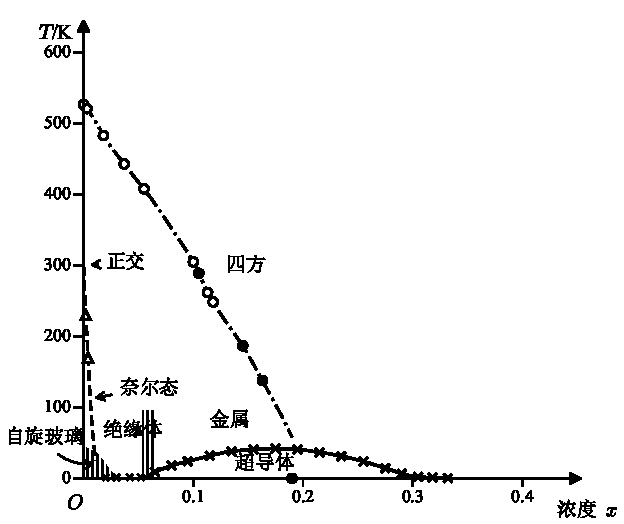
\includegraphics[width=8cm]{fig7-4.pdf}\\{\small 图 7.4\quad $\mathrm{La}_{2-x}\mathrm{Sr}_{x}\mathrm{CuO}_{4}$ 的相图}
\end{minipage}
\end{center}

\begin{center}
\begin{minipage}{8.5cm}
\centering
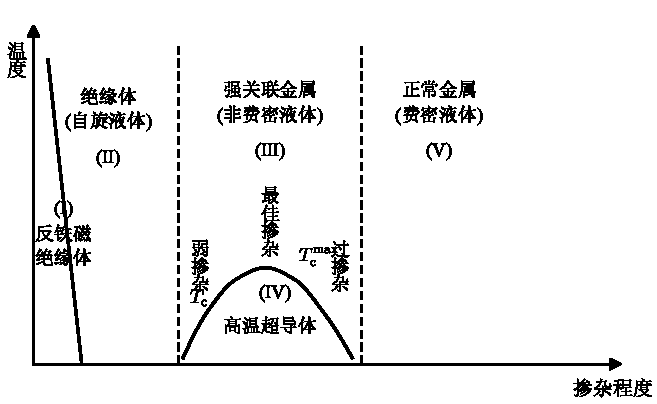
\includegraphics[width=8.5cm]{fig7-5.pdf}\\{\small 图 7.5\quad 氧化物高温超导体的通用相图}
\end{minipage}
\end{center}

(i)母体化合物通常为反铁磁绝缘体，出现在（Ⅰ)区中.

(ii)反铁磁长程序对掺杂极为敏感，当掺杂时反铁磁性迅速消失，取而代之的是高度关联的自旋液体（Ⅱ).

(iii)经绝缘体-金属（I-M）转变，系统进入强关联金属区（Ⅲ)，其特征往往不能用标准的费密液体理论解释.中子衍射实验表明I-M转变对自旋关联并无明显的影响，说明在强关联金属中仍然存在反铁磁自旋关联.

(iv)从强关联金属区域（Ⅲ)降温，系统才能进入高 $T_{\mathrm{c}}$ 超导态区域（Ⅳ).实验还表明，反铁磁自旋关联将一直延伸到高 $T_{\mathrm{c}}$ 超导态中.

(v)进一步掺杂，系统最终进入正常金属区（V)，其特征可用标准费密液体理论中描述，但降温时却不再出现超导电性了.

常规的BCS超导体与氧化物高温超导体最重要的区别在于，BCS超导体的正常态为费密液体，而高 $T_{\mathrm{c}}$ 超导体的正常态为非费密液体.近年来的研究还表明强关联金属区域（Ⅲ)又分为3个区，其中对应于最高转变温度 $T_{\mathrm{c}}$ 的掺杂称为最佳掺杂，掺杂量大于或小于这一数值，分别称为过掺杂与弱掺杂（或欠掺杂），而在这3个区域中正常态的行为有很大的差别，表现在弱掺杂区中出人意料地发现了正常态的能隙，仅当掺杂浓度增加，系统进入最佳掺杂和过掺杂区时，这种异常现象才消失.现已明白，存在正常态能隙是所有铜氧化合物高温超导体在弱掺杂区的普遍特征（详见本章§8），这对理论研究提出了新的挑战.时至今日，如何理解氧化物高 $T_{\mathrm{c}}$ 材料的相图共同特征仍是摆在理论工作者面前的一项基本任务.要建立一个铜氧化合物的超导理论，其主要任务不仅限于解释高 $T_{\mathrm{c}}$ 出现的原因，还应当对上述通用相图（包括弱掺杂区出现正常的能隙）作出全面的解释，这是一个相当高的要求.近年来出现的高温超导电性的SO(5)理论\textsuperscript{[14]}，在研究反铁磁性与高 $T_{\mathrm{c}}$ 超导电性的统一描述方面迈出了重要的一步，值得读者关注.

\section{高温超导体中超导态的基本属性}

在本节中，我们将介绍铜氧化合物超导态的主要特征，并着重于讨论它与BCS超导态的不同之处.

在新发现的铜氧化物高温超导体中，由于对超导配对和正常态输运起关键作用的载流子处于 $\mathrm{CuO}_{2}$ 导电层内，而且这些超导体都具有以 $\mathrm{CuO}_{2}$ 平面为主体的层状结构，普遍认为这些高温超导体的主要物理性质应大致相同.基于这一共识，科学家们将注意力集中于研究某些典型的材料，例如Y-123，因为这类化合物便于制成均匀、纯净和足够大尺寸的单晶，可供标定样品的内在特性.随着样品质量的不断提高和测量手段的不断改进，来自不同研究组的测量数据越来越集中且可靠，对于Y-123甚至达到了彼此定量一致的程度，从而为正确理解高 $T_{\mathrm{c}}$ 铜氧化合物的超导态和正常态属性提供了可靠的依据.对于超导态的基本物理性质，目前已取得共识的主要结果是：

\subsection*{1. 超导态仍然是库柏对的相干凝聚态}

在高温超导体被发现后，随即在诸多的实验中（包括：交流约瑟夫森效应、磁通跳跃、Little-Parks振荡以及磁通量子的直流测量等）均证实了传载超电流的有效电荷为 $e^{*}=2e$\textsuperscript{[15]}，这表明不论是空穴型的、还是电子型的高温超导体仍然是由两个载流配对组成的凝聚体.安德列耶夫（Andreev）反射实验更进一步证实了配对的载流子具有相反的动量和自旋，这与BCS超导态相似，仍然是由（$k\uparrow$）与（$-k\downarrow$）载流子组成的自旋单重态配对——库柏对，而在超导态中传递超电流的有效单元仍应是相位相干的，并已形成了凝聚的库柏对系统，但配对与相干凝聚未必同时发生，也正是在这个意义上我们说，超导仍然是（$k\uparrow$，$-k\downarrow$）载流子对总体的相干凝聚.

人们自然要问及，当高温超导体进入超导状态以后，超导能隙函数的对称性，它涉及超导态的另一个重要特性.

\subsection*{2. 配对的对称性——主要是各向异性的d波配对}

超导能隙函数在物理上代表传递超电流的载流子对（即电子对-电子型，或空穴对-空穴型超导体）波函数的轨道部分，又称超导序参量.由于实验已证实在高温超导体中波函数的自旋部分仍然是奇宇称的自旋单重态，根据全同性原理，能隙函数只能是动量空间中取向 $\hat{\boldsymbol{k}}$ 的偶函数，对应于用球谐函数 $\mathrm{Y}_{lm}(\boldsymbol{k})$ 展开的对波函数轨道部分中取 $l=0,\ 2,\ \cdots$ 等偶宇称解，其中 $l=0$ 情形称为s波配对的各向同性BCS超导体，而 $l=2$ 则称为d波配对的各向异性超导体（在§4将作专门的介绍）.对于BCS超导体，能隙函数在费密面上各方向均取相同的数值 $\Delta$，属于各向同性的s波情形，其中 $2\Delta$ 代表在超导态中折开一个库柏对所需的最小能量，而产生单个准粒子激发所需最小能量为 $\Delta$.由此可知，在BCS超导态中的低温（$T\ll T_{\mathrm{c}}$）元激发密度应与 $\exp(-\beta\Delta)$ 成正比，其中 $\beta=1/k_{\mathrm{B}}T$.当人们测量BCS超导体中的比热容系数和伦敦穿透深度等与元激发密度有关的物理量时，它们在低温下均呈现指数型的温度依赖关系 $\exp(-\beta\Delta)$，这是BCS超导体的一个标志性特征.

对于具有临界温度为40 K以上的各向异性铜氧化合物，为了判断其超导序参量的对称性，至少应当区分下列3种配对，它们分别是：各向同性的s波，$d_{x^{2}-y^{2}}$ 波和各向异性的s波配对，它们在实空间的示意图如图7.6所示.

\begin{center}
\begin{minipage}{8.5cm}
\centering
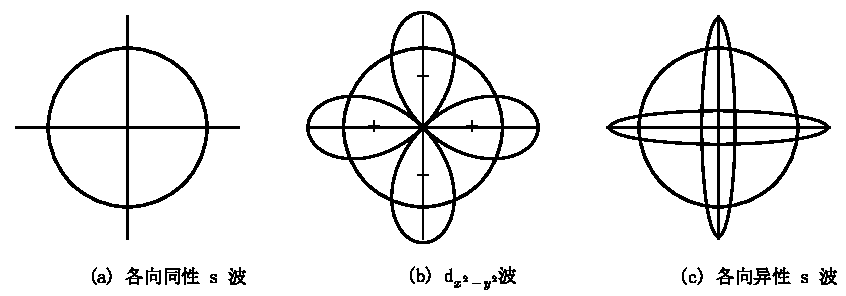
\includegraphics[width=8.5cm]{fig7-6.pdf}\\[0.3em]
{\small (a) 各向同性s波\qquad\quad (b) $d_{x^{2}-y^{2}}$波\qquad\quad (c) 各向异性s波}\\[0.2em]
{\small 图 7.6\quad 超导序参量在实空间中的示意图}
\end{minipage}
\end{center}

早期的实验似乎支持s波图像，包括各向同性的s波［如(a)所示］以及反映超导晶体对称性的各向异性s波配对［如(c)所示］，其中序参量是随着取向变化的，但是序参量的对称性不低于晶体的对称性，仍属于常规s波情形.另一方面，理论工作者也早已提出了 $d_{x^{2}-y^{2}}$ 波配对方案，这是考虑到在 $\mathrm{CuO}_{2}$ 平面内 Cu 的 $d_{x^{2}-y^{2}}$ 轨道电子起主要作用，并且在同一个Cu格点上电子间存在强的同位库仑排斥作用，由于d波配对在粒子间距很小时，对波函数的概率幅也很小，有利于避开高 $T_{\mathrm{c}}$ 氧化物中普遍存在的强同位库仑排斥（简称强关联）作用而形成配对.$d_{x^{2}-y^{2}}$ 波的序参量大小随取向变化，在 $Oxy$ 平面上为四叶草（four-leaf clover）形状，但是 $d_{x^{2}-y^{2}}$ 波不同于各向异性s波的关键性特征是，具有两个正叶和两个负叶，它们的最大数值分别沿x轴和y轴方向，并且沿对角线（$|x|=|y|$ 方向）经过零点，与此同时序参量改变符号，如图7.6(b)所示，各向异性s波的序参量则没有符号的改变，其四个叶瓣均为正，而且沿对角线方向尽管数值很小，但仍为非零，即存在一个最小的实能隙.从对称性分析看，各向异性s波的序参量仍具有超导晶体的4次轴对称，但是 $d_{x^{2}-y^{2}}$ 波（由于存在正、负叶）则无此对称性，其超导序参量的对称性低于超导晶体，被称为非常规配对情形.在动量空间中，超导序参量代表费密面上的能隙函数 $\Delta(\hat{\boldsymbol{k}})$，其中 $\hat{\boldsymbol{k}}\equiv\boldsymbol{k}/\left|\boldsymbol{k}\right|$ 代表沿 k 方向的单位矢量.在二维BZ中，$d_{x^{2}-y^{2}}$ 波的能隙函数可表示为
\begin{equation}
  \Delta(\hat{\boldsymbol{k}})\sim\left(\hat{k}_{x}^{2}-\hat{k}_{y}^{2}\right)=\cos2\phi_{k}\,,\qquad
  \phi_{k}=\arctan\left(\hat{k}_{y}/\hat{k}_{x}\right)
\end{equation}
它不仅随k的取向变化，而且与实空间序参量特性相似，在k空间的某些区域 $\Delta$ 为正，另一些区域 $\Delta$ 为负，沿 $k_{x}$ 和 $k_{y}$ 方向分别取正和负的最大值，并且沿 $|k_{x}|=|k_{y}|$ 方向经过 $\Delta(\hat{\boldsymbol{k}})$ 的零点.能隙函数改变符号和存在零点是 $d_{x^{2}-y^{2}}$ 波配对区别于各向异性s波配对的重要特点.因此，必须直接测量能隙函数 $\Delta(\hat{\boldsymbol{k}})$ 随取向 $\hat{\boldsymbol{k}}$ 的变化，才能从实验上对高温超导体中是否存在非常规的 $d_{x^{2}-y^{2}}$ 波配对作出明确的判断.

角分辨光发射谱仪（ARPES）是一个可以直接测量能隙随取向 $\hat{\boldsymbol{k}}$ 变化的重要手段.1993年斯坦福大学研究组\textsuperscript{[16]}首先发现，在 Bi-Sr-Ca-Cu-O（BSCCO）化合物中，沿 $k_{x}$ 或 $k_{y}$ 方向能隙取最大值，而沿对角线 $|k_{x}|=|k_{y}|$ 方向所测出的能隙值非常小，甚至可以认为是零，具有类似 $d_{x^{2}-y^{2}}$ 波的四叶草形状.类似的结果也在 Y-Ba-Cu-O（YBCO）等化合物中被观测到，但是ARPES测量只能给出沿某个方向能隙的数值 $\left|\Delta(\hat{\boldsymbol{k}})\right|$，而不能辨别能隙的符号取正值还是负值.在这个意义上讲，他们的发现仅仅证明了超导能隙函数是各向异性的，但仍然无法区别 $d_{x^{2}-y^{2}}$ 波和各向异性s波配对，因此，人们又将注意力转向对于能隙 $\Delta$ 的符号改变十分敏感的约瑟夫森结实验.应当明白，超导能隙函数 $\Delta$ 改变符号时，作为一个复序参量函数，相当于 $\Delta$ 的相位改变 $180^{\circ}$，即有相移 $\pi$，人们必须设计出一种能够观测超导序参量相位变化的实验系统.

在相位观测方面，伊利诺斯大学的哈林根（D. V. Harlingen）等人\textsuperscript{[17]}首先作出了贡献，他们用一块常规的BCS超导体铅（Pb）和一块高质量的YBCO单晶做成含有两个约瑟夫森结的超导量子干涉系统，其中各向同性s波超导体 Pb 的两端分别与高温超导体 YBCO 单晶的两个相互垂直的晶面相接触构成约瑟夫森结，组合的构形可参考图7.7(a).如果YBCO也是s波配对，这一组合将不会引入附加的相位差，只能观察到通常的双结量子干涉效应.然而，当YBCO具有 $d_{x^{2}-y^{2}}$ 波对称性时，则将在平行于x（或a）轴的结中出现d波态超导序参量的负叶，而在平行于y（或b）轴的结中出现d波态的正叶，这时YBCO中的负叶将通过相位为各向同性的Pb超导体的连接，面对 YBCO 另一侧的正叶，导致两个结之间有 $\pi$ 相移.在无外磁场时，这一相移 $\pi$ 将使流经两个结的约瑟夫森超电流彼此相消.哈林根等人通过测量临界电流（即最大超电流）与外磁场的关系，在零外场时看到了临界电流的明显相消效应，这是支持d波配对的第一个实验证据.1995年，马里兰大学研究组\textsuperscript{[18]}改用薄膜，而不是块体，构造了与伊利诺斯小组相似的 YBCO-Pb 双结组合，即图7.7(a).他们采用扫描述磁强计直接测出 YBCO-Pb 组合环中的磁通 $\Phi$ 为半整的量子磁通 $\left(n+\dfrac{1}{2}\right)\Phi_{0}$，其中 $\Phi_{0}=\left(\pi\hbar c/e\right)$ 为磁通量子.在这里半个磁通量子 $\left(\dfrac{1}{2}\Phi_{0}\right)$ 的出现是由于 YBCO-Pb 环路中两垂直结之间存在d波相移 $\pi$.为了排除由于结面不平整或含有磁性杂质等偶然因素引起额外的磁通捕获、但却被误认为是d波序参量产生的相移而导致假象的半个磁通量子，马里兰研究组还同时设计了两个结平行于y（即b）轴的组合，如图7.7(b).显然，在(b)组合中两个平行结之间是不存在来自d波配对的相位差，也不会有半整数的量子磁通效应，威尔斯托德（Wellstood）等人在(b)组合中只观察到整数的磁通量子，从而排除了上述偶然因素的影响，与d波配对所预言的结果一致.特别值得一提的是IBM的崔（Tsuei）和克尔特勒（Kirtley）等人的工作\textsuperscript{[19]}，他们利用分子束外延方法首先制了成全由高温超导体YBCO薄膜组成的多结环，在结两侧的YBCO取向不同，可构成 YBCO 中 $d_{x^{2}-y^{2}}$ 配对的正叶直接面对结另一侧YBCO的负叶，形成相移，而无需通过BCS超导体铅作为中介，必然更直接地反映 YBCO 中序参量的对称性.1994年，他们在全由YBCO构成的三结环中首先观察到半个磁通量子的捕获，直接证实了YBCO中为 $d_{x^{2}-y^{2}}$ 波配对，被人们誉为是证实高温超导体为d波配对的里程碑性工作.实验测量还进一步表明，不仅是YBCO，在 Tl-2201 和 BSCCO 等其它的一系列铜氧化物高温超导体中均已证实能隙函数的主导部分都是 $d_{x^{2}-y^{2}}$ 波配对，唯一的例外是电子型的 Nd-Ce-Cu-O 化合物，迄今的实验结果均表明它仍然属于常规的s波配对.

\begin{center}
\begin{minipage}{8cm}
\centering
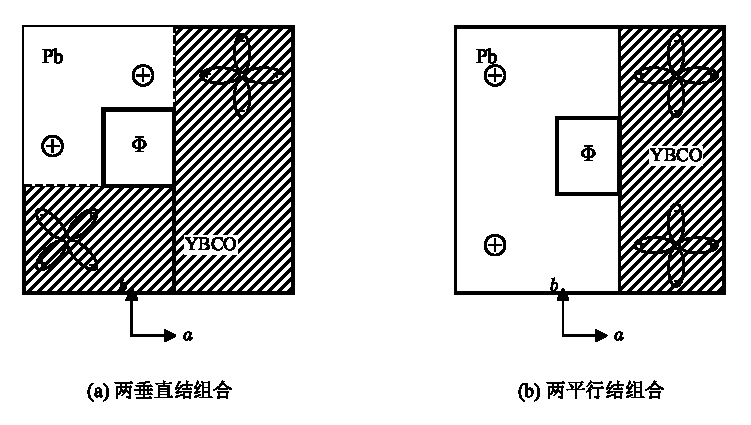
\includegraphics[width=8cm]{fig7-7.pdf}\\[0.3em]
{\small (a) 两垂直结组合\qquad\qquad (b) 两平行结组合}\\[0.2em]
{\small 图 7.7\quad YBCO-Pb 构成的超导量子干涉仪}
\end{minipage}
\end{center}

上面所说的以 $d_{x^{2}-y^{2}}$ 波为主导成分是指，由于实际超导体的配对对称性相当复杂，不排除可能有各向同性s波配对的附加贡献，从而形成混合的 s+d 配对.这类 s+d 混合配对已在YBCO中被观测到，并初步认定是由于各向同性的s波成分的混入，来源于YBCO中存在正交畸变，即当出现超导电性时实际上已是 $a\neq b\neq c$ 的正交晶体\textsuperscript{[20]}.对于不存在正交畸变的 BSCCO 和 Tl-2201 等超导体仍属纯 $d_{x^{2}-y^{2}}$ 波配对，它们的能隙函数都可用式(7.3.1)描述.

\subsection*{3. 极端的Ⅱ类超导体}

铜氧化物高温超导体的明显层状结构将直接影响其超导态中的电子性质，由于这类化合物可以看作为弱耦合 $\mathrm{CuO}_{2}$ 超导层的组合，将导致描述超导电性的参量（如磁穿透深度 $\lambda$ 和超导相干长度 $\xi$ 等）呈现出强烈的各向异性.表7.2中列出了3种氧化物高温超导体在平行于 $\mathrm{CuO}_{2}$ 面（ab平面）和垂直于 $\mathrm{CuO}_{2}$ 面（c方向）的 $\lambda$ 与 $\xi$ 值，其中的 $\xi$ 值是从上临界场 $H_{c2}$ 的测量推算出的G-L相干长度，表中还列出了典型的BCSⅡ类超导体的 $\lambda$ 与 $\xi$ 值，以兹比较.

表7.2\quad 氧化物高温超导体的零温磁穿透深度和G-L相干长度

\begin{center}\small
\begin{tabular}{lcccc}
\hline
化合物 & $\lambda_{ab}(0)$/nm & $\lambda_{c}(0)$/nm & $\xi_{ab}(0)$/nm & $\xi_{c}(0)$/nm\\
\hline
$\mathrm{La}_{2-x}\mathrm{Sr}_{x}\mathrm{CuO}_{4}$ & $800\times10^{-1}$ & $4\,000\times10^{-1}$ & $35\times10^{-1}$ & $7\times10^{-1}$\\
$\mathrm{YBa}_{2}\mathrm{Cu}_{3}\mathrm{O}_{7}$ & $1\,500\times10^{-1}$ & $6\,000\times10^{-1}$ & $15\times10^{-1}$ & $3\times10^{-1}$\\
$\mathrm{Bi}_{2}\mathrm{Sr}_{2}\mathrm{Ca}_{2}\mathrm{Cu}_{3}\mathrm{O}_{10}$ & $2\,000\times10^{-1}$ & $10\,000\times10^{-1}$ & $13\times10^{-1}$ & $2\times10^{-1}$\\
\hline
Nb（Ⅱ类BCS） & \multicolumn{2}{c}{$\lambda=350\times10^{-1}$ nm} & \multicolumn{2}{c}{$\xi=400\times10^{-1}$ nm}\\
\hline
\end{tabular}
\end{center}

除了强各向异性外，所有的氧化物高温超导体由于 $\xi(0)$ 很短，均属于Ⅱ类超导体，其G-L参数
\begin{equation}
  \kappa\equiv\left(\lambda/\xi\right)\gg1/\sqrt{2}
\end{equation}
其中 $1/\sqrt{2}$ 是Ⅱ类超导体的最小 $\kappa$ 值.对于高 $T_{\mathrm{c}}$ 超导材料，$\kappa$ 值超过100，而且由于它们的相干长度 $\xi$ 远远小于 $T_{\mathrm{c}}$ 附近的电子平均自由程 $\left[\left(100\sim200\right)\times10^{-1}\,\mathrm{nm}\right]$，它们是处于干净极限下的极端Ⅱ类超导体.

具体与BCS超导体相比较，氧化物高温超导体的磁穿透深度，即使在 $\mathrm{CuO}_{2}$ 平面内，也相对大一些，这是由于铜氧化合物中的载流子浓度偏低 $\left[n=\left(2\sim5\right)\times10^{21}\,\mathrm{cm}^{-3}\right]$，导致对外磁场屏蔽不足的必然结果.更为突出的是，垂直或平行于 $\mathrm{CuO}_{2}$ 面的相干长度 $\xi_{c}(0)$ 和 $\xi_{ab}(0)$ 比常规BCS超导体的 $\xi$ 要短得多，在氧化物材料中 $\xi(0)$ 的平均值仅为1 nm，和晶胞的尺寸同一量级，只有BCS超导体的1/100～1/10.如此短的平均相干长度 $\xi$，使氧化物高温超导体在相干体积（约 $\xi^{3}$）内只可能含有几个库柏对，与BCS超导体铝（Al）的相体积中有 $10^{4}$ 个库柏对相比较，低了几个数量级，这将使涨落效应变得十分突出.另外，考虑到这里的 $\xi(0)$ 实际上是零温时的G-L相干长度，根据第六章§10的讨论，它实际上代表外扰动所引起超导序参量（或能隙函数）的变化范围或衰减距离，而在铜氧化合物中这个距离很短，甚至单个外来原子也将可能在局部范围内压制掉超导能隙，这又说明高温超导体对于小尺寸的化学结构缺陷将是十分敏感的.

\subsection*{4. 复杂的同位素效应}

在BCS超导体中，同位素效应的实验结果为
\begin{equation}
  T_{\mathrm{c}}\sim M^{-\alpha}
\end{equation}
\begin{equation}
  \alpha=-\frac{\Delta\ln T_{\mathrm{c}}}{\Delta\ln M}
\end{equation}
其中的系数 $\alpha$ 称为同位素指数.显然，$\alpha$ 代表当组成超导体的元素完全被其同位素所代替时，原子质量的相对改变 $\left(\Delta\ln M=\Delta M/M\right)$ 和超导转变温度的相对移动 $\left(\Delta\ln T_{\mathrm{c}}=\Delta T_{\mathrm{c}}/T_{\mathrm{c}}\right)$ 之比值.在历史上，同位素效应的测量是获取配对互作用信息的有力工具，并成功地证实了BCS超导体形成配对的互作用来源于电声子耦合.

实验表明，对于价带由s和p电子组成的金属元素超导体（如 $\mathrm{Hg}$、$\mathrm{Pb}$、$\mathrm{Tl}$、$\mathrm{Sn}$、$\mathrm{Cd}$、$\mathrm{Zn}$ 等）均测得 $\alpha\approx0.5$.这个结果与弱耦合的BCS理论的转变温度公式(6.5.10)所预言的 $T_{\mathrm{c}}\sim\omega_{\mathrm{D}}\sim M^{-1/2}$ 基本上是一致的，对电声子耦合的配对机制给予了有力的支持.但是，同位素效应即使在常规的BCS超导体中也是十分复杂的，例如在过渡金属超导体（Ru、Os 及 Mo）和化合物超导体（$\mathrm{Nb}_{3}\mathrm{Sn}$）中，$\alpha$ 值仅在0～0.3范围之内，明显地偏小，甚至在Ru中几乎观察不到同位素效应（即 $\alpha\approx0$），而在 $\mathrm{Nb}_{3}\mathrm{Sn}$ 中也只有 $\alpha_{\mathrm{Sn}}=0.08$.造成差别的主要原因是巴丁等人在导出式(6.5.10)，即 $k_{\mathrm{B}}T_{\mathrm{c}}=1.13\,\hbar\omega_{\mathrm{D}}\exp\left[-1/g(0)V\right]$ 时，只考虑了在费密面附近厚度为 $2\hbar\omega_{\mathrm{D}}$ 能壳内的净吸引互作用，而忽略了能壳区外实际存在的库仑排斥作用对 $T_{\mathrm{c}}$ 的影响.换句话说，在BCS的弱耦合理论中只取了一个能量切断因子 $\hbar\omega_{\mathrm{D}}$，才能求出 $\alpha$ 的理论值对于所有的超导体均为1/2的简单结果.一种比较合理的计入库仑排斥作用的方案是，除了用 $\hbar\omega_{\mathrm{D}}$ 描述电声子互作用吸引区的切断因子之外，再取一个切断因子描述库仑排斥作用的能区，其大小与费密能 $E_{\mathrm{F}}$ 同量级，且与原子质量M无关.由此即可解释为什么过渡金属及其有关化合物的同位素效应会大幅度地减小.将这一修正方案用于非过渡金属元素的超导体时，也使 $\alpha$ 的理论值更接近实验值，详细的讨论可参阅文献\textsuperscript{[21]}.应当明白，上述理论工作只是改进了巴丁等人对相互作用的过分简化处理，但电子间形成配对的吸引互作用仍由声子作媒介，仍属于电声子机制的超导电性.

由于大多数的BCS元素超导体每元胞中仅含一个原子，其晶格振动谱中仅涉及声学模，可以用德拜模型描述，这时电声机制超导电性主要来自具有最大声子态密度和最高频率 $\omega_{\mathrm{D}}$ 的德拜声子与费密面上电子之间的相互作用.因此，探测其同位素效应只涉及一种原子的同位素替代，比较简单.然而，在新发现的铜氧化物高温超导体都是多元化合物，在每个单胞中均含有多种原子，其晶格振动既有声学模声子，又有频率高低不同的光学模声子，情况将十分复杂.这时测量的同位素指数（$\alpha$）原则上应包括化合物中每个元素的贡献（$\alpha_{i}$），即 $\alpha=\sum_{i}\alpha_{i}$.但是，在氧化物高温超导体中，人们主要是用氧的同位素替代 $^{16}\mathrm{O}$-$^{18}\mathrm{O}$，并测量氧的同位素指数 $\alpha_{0}$，这是出于如下的考虑：从诸元素同位素替代的质量相对改变 $\left(\Delta M_{i}/M_{i}\right)$ 看，对于 $^{16}\mathrm{O}$-$^{18}\mathrm{O}$ 为0.12、$^{63}\mathrm{Cu}$-$^{65}\mathrm{Cu}$ 为0.03、$^{135}\mathrm{Ba}$-$^{138}\mathrm{Ba}$ 为0.02，而对于 $^{138}\mathrm{La}$-$^{139}\mathrm{La}$ 只有0.007，其中以氧为最大.即使在相同 $T_{\mathrm{c}}$ 与 $\alpha_{i}$ 的条件，Cu、Ba、La 等元素的同位素替代所引起的转变温度移动 $\Delta T_{\mathrm{c}}$ 分别只是氧的1/4、1/6 和 1/17.在YBCO这类 $T_{\mathrm{c}}$ 为90 K的氧化物中由于氧的移动已经很小，接近测量的最低极限，其它元素（如 Cu 与 Ba 等）的 $\Delta T_{\mathrm{c}}$ 实际上已难于测出，作为一级近似可以略去，只讨论氧的同位素测量并求其指数 $\alpha_{0}$.在Bi系和Tl系等氧化物中情况也是相似的，人们只测得了氧的同位素效应.唯一的例外是 $T_{\mathrm{c}}$ 较低的La系，其中 $\alpha_{\mathrm{Cu}}$ 与 $\alpha_{0}$ 均已测出，且数值相近，我们将在下文中再作介绍.

实验表明，氧化物高温超导体的同位素效应有如下主要特征\textsuperscript{[22]}：

(i)最佳化合物的 $\alpha_{0}$ 均比BCS的标准值（$\alpha=1/2$）小得多.最佳化合物是其组分具有最高转变温度 $T_{\mathrm{c}}^{\mathrm{max}}$（即最佳掺杂）的化合物，例如 $\mathrm{YBa}_{2}\mathrm{Cu}_{3}\mathrm{O}_{6+x}$ 的 $x=1$ 组分及在 $\mathrm{La}_{2-x}\mathrm{Sr}_{x}\mathrm{CuO}_{4}$ 中的 $x=0.15$ 等组分化合物，表7.3中列出了它们的氧同位素指数 $\alpha_{0}$ 的测量值.

表7.3\quad 最佳化合物的氧同位素效应

\begin{center}\small
\begin{tabular}{lccc}
\hline
铜氧化合物 & $T_{\mathrm{c}}^{\mathrm{max}}$/K & 氧的同位素指数 $\alpha_{0}$ & 超导类型\\
\hline
$\mathrm{La}_{1.85}\mathrm{Sr}_{0.15}\mathrm{CuO}_{4}$ & 40 & 0.10～0.16 & 空穴型\\
$\mathrm{Bi}_{2}\mathrm{Sr}_{2}\mathrm{CaCu}_{2}\mathrm{O}_{8}$ & 85 & 0.03～0.05 & 空穴型\\
$\mathrm{YBa}_{2}\mathrm{Cu}_{3}\mathrm{O}_{7}$ & 90 & 0.02～0.05 & 空穴型\\
$\mathrm{Bi}_{2}\mathrm{Sr}_{2}\mathrm{Ca}_{2}\mathrm{Cu}_{3}\mathrm{O}_{10}$ & 110 & 0.01～0.03 & 空穴型\\
$\mathrm{Tl}_{2}\mathrm{Ba}_{2}\mathrm{Ca}_{2}\mathrm{Cu}_{3}\mathrm{O}_{10}$ & 125 & 0 & 空穴型\\
$\mathrm{Nd}_{1.85}\mathrm{Ce}_{0.15}\mathrm{CuO}_{4}$ & 24 & $<$0.05 & 电子型\\
\hline
\end{tabular}
\end{center}

若比较表7.3中诸空穴型氧化物超导体的 $T_{\mathrm{c}}^{\mathrm{max}}$ 和 $\alpha_{0}$，可以看出 $\alpha_{0}$ 随 $T_{\mathrm{c}}^{\mathrm{max}}$ 上升而迅速减小，除La系以外，在其它的 $T_{\mathrm{c}}>85$ K 超导体中 $\alpha_{0}$ 均很小，说明它们的同位素效应非常弱.这是氧化物高温超导体同位素效应与BCS超导体的主要区别，也是人们在高温超导体发现之后就相信它们不是声子机制超导体的主要原因.尽管有人将电声子机制的强耦合超导理论用于 La-Sr 系最佳化合物，求得了与表7.3中 $\alpha_{0}$ 实验值一致的结果，但是若将此理论用于Y-123等最佳化合物，却不能同时解释高的转变温度（$T_{\mathrm{c}}^{\mathrm{max}}=90$ K）和极其微小的 $\alpha_{0}$ 值（0.02～0.05）.电声子机制超导理论对高 $T_{\mathrm{c}}^{\mathrm{max}}$ 最佳化合物运用的失败，推动了人们对非声子机制的探索，支持这种观点的科学家认为在铜氧化合物中，至少电声子耦合不是形成超导的主要原因，而超导配对应来源于载流子之间交换其它类型的玻色子，这些玻色子可能是由电子性或磁性元激发所产生的，其中最著名是有利于形成 $d_{x^{2}-y^{2}}$ 波配对的反铁磁自旋涨落模型\textsuperscript{[23]}.

对最佳化合物进行掺杂，超导转变温度 $T_{\mathrm{c}}$ 将偏离其最大值 $T_{\mathrm{c}}^{\mathrm{max}}$ 而下降，这时氧的同位素效应明显地增大，在氧化物高温超导体中，同位素指数 $\alpha_{0}$ 随掺入空穴的浓度变化是它们不同于BCS超导体的另一反常特征，在BCS理论中 $\alpha$（$\alpha=1/2$）是一个与载流子浓度无关的常数.

(ii)$\alpha_{0}$ 的大小明显地依赖于空穴浓度，在增加或减小掺入空穴（即在过掺杂或弱掺杂）情况下，$\alpha_{0}$ 均呈现增大的趋势，有时可以接近甚至超过BCS的标准值0.5.例如，在 $\mathrm{YBa}_{2-x}\mathrm{La}_{x}\mathrm{Cu}_{3}\mathrm{O}_{7}$ 掺杂系统中，由于是用 $\mathrm{La}^{3+}$ 取代电子库中的 $\mathrm{Ba}^{2+}$，其主要作用是减少空穴浓度，实验测出的 $\alpha_{0}$ 随x的增加将单调地上升，到 $x=0.5$ 时可达 $\alpha_{0}=0.38$，这是弱掺杂情形.对于增加空穴浓度的过掺杂情形，已在 $\left(\mathrm{Y}_{1-x}\mathrm{Pr}_{x}\right)\mathrm{Ba}_{2}\mathrm{Cu}_{3}\mathrm{O}_{7}$ 等掺杂系统中被观察到.在Y-123掺 Pr（+3.8价）体系中，$\alpha_{0}$ 仍然是随掺杂增大，当 Pr 的浓度 $x=0.5$ 时，氧的同位素指数已超过BCS标准值（1/2），达到 $\alpha_{0}=0.55$.类似的 $\alpha_{0}$ 对空穴浓度的依赖关系也在 Bi-2212 等化合物中被看到.因此，尽管 $T_{\mathrm{c}}^{\mathrm{max}}$ 较高的最佳化合物中只观测到很小的同位素效应，但掺杂使之偏离最佳浓度后又能普遍地观察到显著的氧同位素效应和较高的 $\alpha_{0}$ 值，这表明同位素效应对各种相互作用均十分敏感，在过掺杂或弱掺杂区域中讨论同位素效应时电声子互作用的影响是不可忽略的.掺杂 La-214 系统的同位素效应，除具有以上特征外还有某些独特之处，有必要作单独介绍.

(iii)$\mathrm{La}_{2-x}\mathrm{M}_{x}\mathrm{CuO}_{4}$（M=Sr，Ba）系统中同位素效应随掺杂浓度的变化十分特别，在最佳掺杂浓度 $x=0.15$ 处，$T_{\mathrm{c}}^{\mathrm{max}}$ 接近40 K，$\alpha_{0}$ 很小，只有0.1，这是La-214的主要特点.当x略低于最佳浓度时，$\alpha_{0}$ 迅速上升，当 $x=0.125$ 时可高达 $\alpha=0.8$.然后，又随x减小而下降，当 $x=0.075$ 时，$\alpha_{0}=0.4$.图7.8是La-214中掺Sr时的 $T_{\mathrm{c}}$ 和 $\alpha_{0}$ 随x变化曲线.另外，在图7.9中还给出了铜的同位素指数 $\alpha_{\mathrm{Cu}}$.

\begin{center}
\begin{minipage}{7.5cm}
\centering
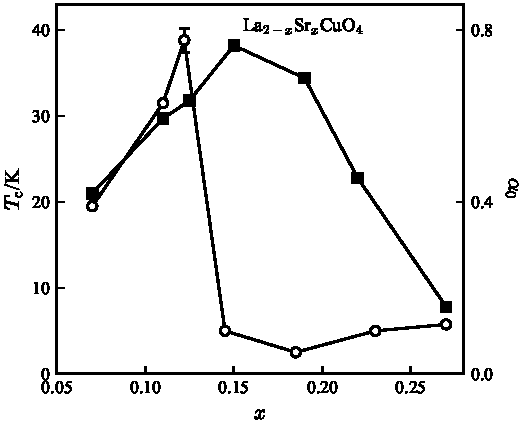
\includegraphics[width=7.5cm]{fig7-8.pdf}\\{\small 图 7.8\quad $\mathrm{La}_{2-x}\mathrm{Sr}_{x}\mathrm{CuO}_{4}$ 中 $T_{\mathrm{c}}$（■）和 $\alpha_{0}$（○）随 Sr 含量的变化关系}
\end{minipage}
\end{center}

在图7.9中，$\alpha_{\mathrm{Cu}}$ 也是从0.1（当 $x=0.15$ 时）迅速上升到0.8（当 $x=0.125$ 时）.此外，还可以清楚地看到，在La-214中无论是掺Ba或者是掺Sr，$\alpha_{0}$ 随x的变化落在同一条曲线上，考虑到 Sr 与 Ba 的质量相差颇大，但 $\alpha_{0}$ 的尖峰却都位于同一点（$x=1/8$ 处），我们完全有理由认为这一尖峰行为来源于电子效应，极有可能是和 $\mathrm{CuO}_{2}$ 电子态密度的尖峰（即近半满的二维布里渊区中电子态密度的范·霍夫奇性）有关.理论工作者在BCS声子机制范围内计入范·霍夫奇性对掺杂 La-214 系统的 $T_{\mathrm{c}}$ 和 $\alpha$ 的影响\textsuperscript{[24]}，解释了掺杂 La-214 中这一反常同位素效应，但却限于s波配对和电声子机制，不能全面地解释 La-214 铜氧化物的其它超导特征（如d波配对等）.换句话说，仅仅对同位素效应的反常作出解释仍不足以证实高温超导电性来源于电声子机制.

\begin{center}
\begin{minipage}{7.5cm}
\centering
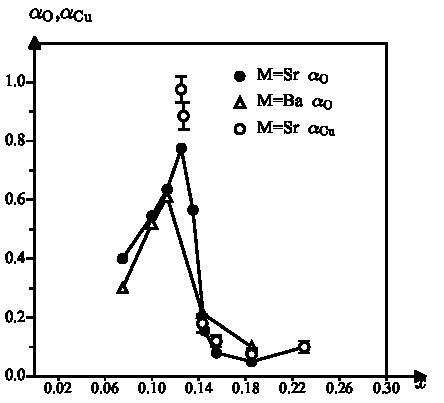
\includegraphics[width=7.5cm]{fig7-9.pdf}\\{\small 图 7.9\quad $\mathrm{La}_{2-x}\mathrm{M}_{x}\mathrm{CuO}_{4}$ 中的 $\alpha_{0}$、$\alpha_{\mathrm{Cu}}$ 随 x 变化曲线}
\end{minipage}
\end{center}

根据同位素效应的现有实验结果，人们既不能肯定，也不能否定高温超导电性来源于声子机制.尽管如此，在高温超导体中毕竟观察到了有限的 $\alpha$ 值，它至少暗示着在超导配对和凝聚的机制中包含有受声子效应影响的因素，有可能不是主要

的决定配对和凝聚的因素，但在解释同位素效应时却是不可忽略的.还应当指出，在La-214中观察到 $\alpha_{\mathrm{Cu}}$ 与 $\alpha_{0}$ 具有相同的数量级，表明当讨论电声子互作用对超导电性的影响时，$\mathrm{CuO}_{2}$ 平面上铜和氧离子的晶格振动是同等重要的.

最后，对常规和高温超导体中复杂的同位素效应作一个简单的小结.在常规的电声子机制BCS超导体中，尽管电性的库仑作用的影响曾使同位素效应变得十分复杂，但总趋势仍是以 $\alpha\approx1/2$ 的电声子机制为主导.目前，在高温超导体中的总趋势仍然是同位素效应普遍偏小，尽管在某些特殊情况下（如在弱掺杂区）声子效应不可忽略，使问题变得十分复杂，但是历史是值得借鉴的，作者仍相信配对的主要机制不是电声子互作用.

\subsection*{5. 不同于BCS超导体的低温特性}

除了 Nd-Ce-Cu-O 化合物以外，所有的铜氧化物高温超导体在 $T\ll T_{\mathrm{c}}$ 时均显示出与BCS超导体十分不同的特征.特别是超导态的低温电子比热容 $c_{\mathrm{s}}\left(T\ll T_{\mathrm{c}}\right)$、核自旋-点阵弛豫率 $T_{1\mathrm{s}}^{-1}\left(T\ll T_{\mathrm{c}}\right)$ 和伦敦穿透深度的变化 $\Delta\lambda(T)\equiv\lambda_{\mathrm{L}}(T)-\lambda_{\mathrm{L}}(0)$ 等物理量都表现为随温度变化的 $T^{n}$ 型简单幂次规律，而不是各向同性BCS超导体的 $\exp\left[-\Delta(0)/k_{\mathrm{B}}T\right]$ 型的指数激发特征.表7.4中列出了实验测量的结果，它们实际上是d波配对特征的反映.

表7.4\quad $T\ll T_{\mathrm{c}}$ 时高温超导体和BCS超导体的特性比较

\begin{center}\small
\begin{tabular}{lcc}
\hline
低温物性 & 高温超导体 & BCS超导体\\
\hline
$c_{\mathrm{s}}\left(T\ll T_{\mathrm{c}}\right)$ & $\sim T^{2}$ & $\sim\mathrm{e}^{-\Delta(0)/k_{\mathrm{B}}T}$\\
$\Delta\lambda\left(T\ll T_{\mathrm{c}}\right)$ & $\sim T$（$T^{2}$ 含杂） & $\sim\mathrm{e}^{-\Delta(0)/k_{\mathrm{B}}T}$\\
$T_{1\mathrm{s}}^{-1}\left(T\ll T_{\mathrm{c}}\right)$ & $\sim T^{3}$（$^{63}$Cu） & $\sim T\mathrm{e}^{-\Delta(0)/k_{\mathrm{B}}T}$\\
\hline
\end{tabular}
\end{center}

为了说明以上异常的低温特性，我们将先介绍各向异性超导电性，然后在§6中利用d波配对的超导理论作具体的解释.

\section{各向异性配对的超导电性}

上一章介绍的BCS超导理论是假定在费密面附近电子间的有效互作用矩阵元 $V\left(\boldsymbol{k},\boldsymbol{k}'\right)\approx-V$，即在能壳区内存在一个近似为常数的吸引势（$-V$）.这类吸引来源于电子间交换虚声子所形成的均匀净吸引互作用.按照此简化假定，求出的库柏对（也就是自旋单重态 $\left(\uparrow\downarrow-\downarrow\uparrow\right)/\sqrt{2}$ 配对）波函数和多体系统的能隙函数 $\Delta$ 均与电子间取向 $\left(\theta,\varphi\right)$ 无关，人们往往称之为各向同性超导体.近年来，大量实验事实已证明，还存在各向异性配对的超导体或超流体，其超导或超流序参量（即能隙函数）随取向 $\left(\theta,\varphi\right)$ 强烈变化，又称为各向异性配对超导（或超流）系统.在这类系统中，费密子间配对的自旋态既可能是单重态：$\left(\uparrow\downarrow-\downarrow\uparrow\right)/\sqrt{2}$，也可能是三重态：$\uparrow\uparrow$、$\downarrow\downarrow$ 及 $\left(\uparrow\downarrow+\downarrow\uparrow\right)/\sqrt{2}$.这时导致配对的主要相互作用不再是来源于交换虚声子，而是由于费密子间的强烈同位（即同一格点上的）库仑排斥作用（又称强关联）所激发的其它类型的波色子传递而形成的有效互作用.例如，在超流 $^{3}\mathrm{He}$ 系统中所形成的核自旋三重态各向异性配对来源于 $^{3}\mathrm{He}$ 原子间交换铁磁性自旋涨落，而在重费密子系统及氧化氧高温超导体中的发现的自旋单重态各向异性d波配对超导电性，尽管其微观机理至今尚未确定，但是强同位库仑关联所激发的反铁磁自旋涨落至少可认为是有利于形成各向异性d波配对的一种可能机制.

为了研究各向异性配对超导或超流，有必要将BCS理论推广用于任意有效互作用和任意自旋取向配对情形.为使物理图像明确，先讨论单个对（即广义的库柏对）问题，然后再推广到多体系统求能隙函数.

\subsection*{1. 广义库柏对}

现在将第六章§3中所讨论的一对自旋取向反平行电子之间配对的库柏问题推广到包括自旋平行与反平行配对的一般情形.类似于习题(27)，在这里仍讨论在填满的费密球之外存在两个相互作用的费密子的量子力学问题.不同之处在于它们是具有任意自旋取向的两个费密子 $\left(\boldsymbol{r}_{1},\sigma_{1}\right)$ 与 $\left(\boldsymbol{r}_{2},\sigma_{2}\right)$，其间仅在费密面外 $\hbar\omega_{0}$ 宽度的能壳区内存在有效互作用 $V\left(\left|\boldsymbol{r}_{1}-\boldsymbol{r}_{2}\right|\right)$，这时两费密子系统的波函数 $\psi\left(\boldsymbol{r}_{1}\sigma_{1};\boldsymbol{r}_{2}\sigma_{2}\right)$ 满足定态薛定谔方程
\begin{equation}
  \left\{-\left(\hbar^{2}/2m\right)\left(\nabla_{1}^{2}+\nabla_{2}^{2}\right)
  +V\left(\left|\boldsymbol{r}_{1}-\boldsymbol{r}_{2}\right|\right)-E'\right\}
  \psi\left(\boldsymbol{r}_{1}\sigma_{1};\boldsymbol{r}_{2}\sigma_{2}\right)=0
\end{equation}
在质心动量等于零时，是一对动量相反的费密子（即取 $\boldsymbol{k}_{1}+\boldsymbol{k}_{2}=\boldsymbol{0}$），这时二体波函数可简单地写为
\begin{equation}
  \psi\left(\boldsymbol{r}_{1}\sigma_{1};\boldsymbol{r}_{2}\sigma_{2}\right)
  =\varphi\left(\boldsymbol{r}_{1}-\boldsymbol{r}_{2}\right)\chi\left(\sigma_{1},\sigma_{2}\right)
\end{equation}
其中空间部分只是相对坐标 $\boldsymbol{r}=\boldsymbol{r}_{1}-\boldsymbol{r}_{2}$ 的函数.由于 $\psi$ 应具有全同费密子系统的反对称特征，当自旋波函数 $\chi\left(\sigma_{1},\sigma_{2}\right)$ 为单重态时，其轨道部分 $\varphi\left(\boldsymbol{r}_{1}-\boldsymbol{r}_{2}\right)$ 必须为 $\boldsymbol{r}_{1}-\boldsymbol{r}_{2}$ 的偶函数，这是偶宇称情形，而当 $\chi\left(\sigma_{1},\sigma_{2}\right)$ 为自旋三重态时，则要求 $\varphi\left(\boldsymbol{r}_{1}-\boldsymbol{r}_{2}\right)$ 为奇函数，属于奇宇称情形.

由于有效势V与自旋无关，式(7.4.1)在相对坐标（$\boldsymbol{r}\equiv\boldsymbol{r}_{1}-\boldsymbol{r}_{2}$）中可用 $\varphi(\boldsymbol{r})$ 表示
\begin{equation}
  \left[-\left(\hbar^{2}/m\right)\nabla^{2}+V(\boldsymbol{r})\right]\varphi(\boldsymbol{r})=E'\varphi(\boldsymbol{r})
\end{equation}
其中 $\varphi(\boldsymbol{r})$ 代表相对运动的轨道波函数.对 $\varphi(\boldsymbol{r})$ 作傅里叶变换
\begin{equation}
  \varphi(\boldsymbol{r})=\sum_{\boldsymbol{k}}\varphi(\boldsymbol{k})\,\mathrm{e}^{\mathrm{i}\boldsymbol{k}\cdot\boldsymbol{r}}
\end{equation}
并写出有效互作用的矩阵元
\begin{equation}
  V\left(\boldsymbol{k},\boldsymbol{k}'\right)=\int\mathrm{d}^{3}r\,
  \mathrm{e}^{-\mathrm{i}\left(\boldsymbol{k}-\boldsymbol{k}'\right)\cdot\boldsymbol{r}}V(\boldsymbol{r})
\end{equation}
则式(7.4.3)变为
\begin{equation}
  \left(2E_{k}-E'\right)\varphi(\boldsymbol{k})=-\sum_{\boldsymbol{k}'}V\left(\boldsymbol{k},\boldsymbol{k}'\right)\varphi(\boldsymbol{k}')
  \qquad\left[E_{k}\equiv\left(\hbar^{2}k^{2}/2m\right)\right]
\end{equation}
取费密能 $E_{\mathrm{F}}=\left(\hbar^{2}k_{\mathrm{F}}^{2}/2m\right)$ 作为能量的原点，并定义
\begin{equation}
  \varepsilon_{k}\equiv E_{k}-E_{\mathrm{F}}\ ,\quad E\equiv E'-2E_{\mathrm{F}}
\end{equation}
可将式(7.4.6)改写为
\begin{equation}
  \left(2\varepsilon_{k}-E\right)\varphi(\boldsymbol{k})=-\sum_{\boldsymbol{k}'}V\left(\boldsymbol{k},\boldsymbol{k}'\right)\varphi(\boldsymbol{k}')
\end{equation}
当基体材料为各向同性时，$V\left(\boldsymbol{k},\boldsymbol{k}'\right)$ 只是 $\left|\boldsymbol{k}-\boldsymbol{k}'\right|=k^{2}+k'^{2}-2kk'\cos\theta_{\boldsymbol{k}\boldsymbol{k}'}$ 的函数，并且由于V仅在费密面附近不为零，可近似取 $k=k'=k_{\mathrm{F}}$，这时 $V\left(\boldsymbol{k},\boldsymbol{k}'\right)$ 只是 k 与 $\boldsymbol{k}'$ 费密子间夹角余弦 $\cos\theta_{\boldsymbol{k}\boldsymbol{k}'}$ 的函数.按此，V可用勒让德函数展开
\begin{equation}
  V\left(\boldsymbol{k},\boldsymbol{k}'\right)=V\left(\hat{\boldsymbol{k}}\cdot\hat{\boldsymbol{k}}'\right)
  =V\left(\cos\theta_{\boldsymbol{k}\boldsymbol{k}'}\right)
  =\sum_{l}\left(2l+1\right)V_{l}\,\mathrm{P}_{l}\left(\cos\theta_{ll'}\right)
\end{equation}
其中 $\hat{\boldsymbol{k}}$ 为k方向的单位矢，而l分波势
\begin{equation}
\begin{aligned}
  V_{l}&=\frac{1}{2}\int_{-1}^{1}\mathrm{d}\left(\cos\theta_{\boldsymbol{k}\boldsymbol{k}'}\right)
  V\left(\cos\theta_{\boldsymbol{k}\boldsymbol{k}'}\right)\mathrm{P}_{l}\left(\cos\theta_{\boldsymbol{k}\boldsymbol{k}'}\right)\\
  &=\int_{\mathrm{FS}}\frac{\mathrm{d}\Omega}{4\pi}\,V\left(\boldsymbol{k},\boldsymbol{k}'\right)\mathrm{P}_{l}\left(\cos\theta_{\boldsymbol{k}\boldsymbol{k}'}\right)
\end{aligned}
\end{equation}
显然 $V_{l}$ 是一个只与 $k_{\mathrm{F}}$ 有关的常数，它仅在费密球外 $0\leqslant\varepsilon_{k}\leqslant\hbar\omega_{0}$ 能壳内不为零.利用数学等式
\begin{equation}
  \mathrm{P}_{l}\left(\cos\theta_{\boldsymbol{k}\boldsymbol{k}'}\right)=\frac{4\pi}{\left(2l+1\right)}
  \sum_{m=-l}^{l}\mathrm{Y}_{lm}\left(\theta_{\boldsymbol{k}},\phi_{\boldsymbol{k}}\right)
  \mathrm{Y}_{lm}^{*}\left(\theta_{\boldsymbol{k}'},\phi_{\boldsymbol{k}'}\right)
\end{equation}
其中 $\left(\theta_{\boldsymbol{k}},\phi_{\boldsymbol{k}}\right)$ 与 $\left(\theta_{\boldsymbol{k}'},\phi_{\boldsymbol{k}'}\right)$ 分别代表 k 与 $\boldsymbol{k}'$ 的方位角，将式(7.4.9)与式(7.4.11)代入式(7.4.8)，并利用谐球函数 $\mathrm{Y}_{lm}$ 的正交归一性
\begin{equation}
\begin{aligned}
  \delta_{ll'}\delta_{mm'}&=\int\mathrm{d}\Omega\,\mathrm{Y}_{lm}^{*}\left(\theta_{\boldsymbol{k}},\phi_{\boldsymbol{k}}\right)
  \mathrm{Y}_{l'm'}\left(\theta_{\boldsymbol{k}},\phi_{\boldsymbol{k}}\right)\\
  &=\int_{0}^{\pi}\mathrm{d}\theta_{\boldsymbol{k}}\int_{0}^{2\pi}\mathrm{d}\phi_{\boldsymbol{k}}\,
  \mathrm{Y}_{lm}^{*}\left(\theta_{\boldsymbol{k}},\phi_{\boldsymbol{k}}\right)
  \mathrm{Y}_{l'm'}\left(\theta_{\boldsymbol{k}},\phi_{\boldsymbol{k}}\right)
\end{aligned}
\end{equation}
容易证明，对于确定的l与m，式(7.4.8)的本征函数 $\varphi(\boldsymbol{k})$ 可简单取下列特解：
\begin{subequations}
\begin{equation}
  \varphi(\boldsymbol{k})=\psi_{l}(\boldsymbol{k})\,\mathrm{Y}_{lm}\left(\theta_{\boldsymbol{k}},\phi_{\boldsymbol{k}}\right)
\end{equation}
其中l分波的振幅 $\psi_{l}(\boldsymbol{k})$（$k=\left|\boldsymbol{k}\right|$ 与方位无关）满足方程
\begin{equation}
\begin{aligned}
  \left(2\varepsilon_{k}-E\right)\psi_{l}(k)
  &=-\frac{V_{l}}{\left(2\pi\right)^{3}}\int_{\varepsilon_{k'}=0}^{\varepsilon_{k'}=\hbar\omega_{0}}
  4\pi k'^{2}\psi_{l}(k')\,\mathrm{d}k'\\
  &=-V_{l}\sum_{k>k_{\mathrm{F}}}\psi_{l}(k')
  \qquad\left(0\leqslant\varepsilon_{k'}\leqslant\hbar\omega_{0}\right)
\end{aligned}
\end{equation}
\end{subequations}
令 $\sum\limits_{k'>k_{\mathrm{F}}}\psi_{l}(k')\equiv A$，代入式(7.4.13b)，得到 $\psi_{l}(k)=-V_{l}A/\left(2\varepsilon_{k}-E\right)$，再对k求和，可求出对于A的非零解应满足下列自洽方程：
\begin{equation}
  1=-V_{l}\sum_{k>k_{\mathrm{F}}}\frac{1}{2\varepsilon_{k}-E}
  \qquad\left(0\leqslant\varepsilon_{k}\leqslant\hbar\omega_{0}\right)
\end{equation}
考虑到 $\hbar\omega_{0}\ll E_{\mathrm{F}}$，上式可近似为
\begin{equation}
  1=-g(0)V_{l}\int_{0}^{\hbar\omega_{0}}\frac{\mathrm{d}\varepsilon}{2\varepsilon-E}
  =-g(0)V_{l}\ln\left(\frac{2\hbar\omega_{0}-E}{-E}\right)
\end{equation}
显然，当 $V_{l}<0$ 时，求出的能量 $E<0$，这时E代表l分波配对态的能量
\begin{equation}
  E=-\frac{2\hbar\omega_{0}}{\exp\left[2/g(0)\left|V_{l}\right|\right]-1}
\end{equation}
即使当吸引互作用很弱且满足 $g(0)\left|V_{l}\right|\ll1$ 时，也可得到类似(6.3.11)的束缚对态
\begin{equation}
  E=-2\hbar\omega_{0}\exp\left[-2/g(0)\left|V_{l}\right|\right]<0
\end{equation}
说明形成了l分波的束缚对.以上讨论表明：通常只需在 $V\left(\boldsymbol{k},\boldsymbol{k}'\right)$ 的分波展开式(7.4.9)中取最大 $\left|V_{l}\right|$ 的吸引项，即可构成l分波配对的束缚态 $E<0$，它反而比费密球内侧无相互作用的电子对能量还要低，这自然将使费密球内侧的电子自动溢出，从而导致费密球态失稳，这是形成l波配对超导的信号.由于l分波的k空间波函数为 $\varphi(\boldsymbol{k})=\psi_{l}(k)\mathrm{Y}_{lm}\left(\theta_{\boldsymbol{k}},\phi_{\boldsymbol{k}}\right)$，显然只要 $l>0$，$\varphi(\boldsymbol{k})$ 就是随方位 $\theta_{\boldsymbol{k}}$ 与 $\phi_{\boldsymbol{k}}$ 变化的各向异性函数，因此 $l>0$ 分波配对又可称为各向异性配对.

现在进一步讨论配对态轨道部分的宇称与 $\varphi(\boldsymbol{k})$ 的关系.前文中已指出，当配对费密子的自旋处于单重态时，$\varphi\left(\boldsymbol{r}=\boldsymbol{r}_{1}-\boldsymbol{r}_{2}\right)$ 为偶函数，其傅里叶变换也应为k的偶函数，这时轨道部分只能取 $\mathrm{Y}_{lm}$ 中 $l=0,\ 2,\ \cdots$ 诸偶数.反之，配对费密子的自旋取三重态时，由于要求轨道部分 $\varphi\left(\boldsymbol{r}\right)$ 为r的奇函数，则 $\varphi(\boldsymbol{k})$ 就只能取 $\mathrm{Y}_{lm}$ 中 $l=1,\ 3,\ 5,\ \cdots$ 诸奇数，构成k的奇函数.以上讨论可归结为

表7.5

\begin{center}\small
\begin{tabular}{lcc}
\hline
 & 自旋单重态 & 自旋三重态\\
\hline
自旋波函数 $\chi\left(\sigma_{1},\sigma_{2}\right)$ &
$\left(\uparrow\downarrow-\downarrow\uparrow\right)/\sqrt{2}$ &
$\uparrow\uparrow$，$\downarrow\downarrow$，$\left(\uparrow\downarrow+\downarrow\uparrow\right)/\sqrt{2}$\\
轨道波函数 $\mathrm{Y}_{lm}\left(\theta_{\boldsymbol{k}},\phi_{\boldsymbol{k}}\right)$ &
$l=$ 偶数 $\left(0,2,4,\cdots\right)$ & $l=$ 奇数 $\left(1,3,5,\cdots\right)$\\
 & s波 $\left(l=0\right)$，d波 $\left(l=2\right)$ & p波 $\left(l=1\right)$\\
\hline
轨道宇称 & 偶 & 奇\\
\hline
\end{tabular}
\end{center}

由此可知，除了 $l=0$ 的s波配对是各向同性配对以外，所有的 $l>0$ 分波，其 $\varphi(\boldsymbol{k})$ 均按 $\mathrm{Y}_{lm}\left(\theta_{\boldsymbol{k}},\phi_{\boldsymbol{k}}\right)$ 随k的方位变化.推广到多个对情形，其能隙函数也应当是随方位 $\hat{\boldsymbol{k}}$（$\hat{\boldsymbol{k}}\equiv\boldsymbol{k}/\left|\boldsymbol{k}\right|$）变化的函数，这就是各向异性超导体的特征.

在实际计算时，应具体给出有效势 $V(\boldsymbol{r})$ 及其矩阵元 $V\left(\boldsymbol{k},\boldsymbol{k}'\right)$.在 $^{3}\mathrm{He}$ 液体中，实验已证实超流来源于两个 $^{3}\mathrm{He}$ 原子核自旋的三重态配对，其轨道部分为 $l=1$ 的p波配对.理论上，人们计算出在 $^{3}\mathrm{He}$ 原子间交换铁磁（FM）自旋涨落时，有效势的诸分量中 $V_{l=1}<0$，且其数值 $\left|V_{1}\right|$ 为最大，这将导致轨道部分形成奇宇称的p波配对.在高温超导体中，实验已证实轨道部分主要是d波偶宇称配对.理论上人们用强关联模型解释，因为强关联体系的特征是存在很强的同位库仑排斥作用，它将阻止s波配对的形成，由于s轨道的径向波函数在r较小时仍然很大，同位库仑关联对s波配对的影响将是十分显著的.但是强关联的理论却允许形成d波配对，因为在量子力学中已知，d轨道的径向波函数在r很小时存在零点，因此即使在强关联存在时，同位库仑排斥作用也不会对d波产生显著的影响，这就是在铜氧化物强关联体系中有利于形成d波配对的原因.至于重费密子体系，尽管实验尚无定论，但多数研究者认为配对的吸引作用来源于重费密子间交换反铁磁（AFM）自旋涨落，并已证明在这种有效互作用势中 $V_{l=2}$ 为最大吸引分波势，从而预言重费密子超导体中也是以d波配对为主导的各向异性超导体.

\subsection*{2. 各向异性能隙函数}

现在将上述理论推广到多体系统，求解各向异性超导体的能隙函数.为简单起见，我们仅限于讨论自旋反平行电子间的单重态配对，因为实验已证明氧化物高温超导体中仍是 $\uparrow$，$\downarrow$ 自旋电子间配对所形成的各向异性超导体.设形成超导的有效互作用为
\begin{equation}
  H_{\mathrm{eff}}=\sum_{k,k'}V\left(\boldsymbol{k},\boldsymbol{k}'\right)C^{+}_{k'}C^{+}_{-k'}C_{-k}C_{k}
\end{equation}
其中仍系采用简化记号 $k\equiv\left(\boldsymbol{k},\uparrow\right)$，$-k\equiv\left(-\boldsymbol{k},\downarrow\right)$.有效互作用矩阵元 $V\left(\boldsymbol{k},\boldsymbol{k}'\right)$ 仍由式(7.4.5)描述，它只是 k 与 $\boldsymbol{k}'$ 间夹角余弦的函数，可根据式(7.4.9)作分波展开，并且仅在费密面附近能壳区 $-\hbar\omega_{0}\leqslant\varepsilon_{k},\varepsilon_{k}\leqslant\hbar\omega_{0}$ 内不为零.式(7.4.18)与BCS有效互作用式(6.2.8)之差别在于，现在的 $V\left(\boldsymbol{k},\boldsymbol{k}'\right)=V\left(\hat{\boldsymbol{k}}\cdot\hat{\boldsymbol{k}}'\right)$ 是各向异性的，而不再取BCS的各向同性s波分波势假定 $V\left(\boldsymbol{k},\boldsymbol{k}'\right)=-V$.

当存在自旋单重态配对时，费密面附近一对动量与自旋取向均相反的电子间将形成 $\left(\boldsymbol{k}\uparrow,-\boldsymbol{k}\downarrow\right)$ 型库柏对，使对算符的下列平均不为零
\begin{equation}
  \langle C_{-k}C_{k}\rangle_{T}\neq0\,,\qquad
  \langle C^{+}_{k}C^{+}_{-k}\rangle_{T}\neq0
\end{equation}
在自洽场近似下，与式(6.4.4)对应的约化哈密顿量为
\begin{equation}
\begin{aligned}
  \overline{H}&=\sum_{k}\varepsilon_{k}\left(C^{+}_{k}C_{k}+C^{+}_{-k}C_{-k}\right)
  +\sum_{k,k'}V\left(\boldsymbol{k},\boldsymbol{k}'\right)\left\{C^{+}_{k}C^{+}_{-k}\langle C_{-k'}C_{k'}\rangle_{T}\right.\\
  &\quad\left.+C_{-k}C_{k}\langle C^{+}_{k'}C^{+}_{-k'}\rangle_{T}\right\}
  -\sum_{k,k'}V\left(\boldsymbol{k},\boldsymbol{k}'\right)
  \langle C^{+}_{k'}C^{+}_{-k'}\rangle_{T}\langle C_{-k}C_{k}\rangle_{T}
\end{aligned}
\end{equation}
类似于式(6.4.5)，定义各向异性的能隙函数
\begin{equation}
  \Delta(\boldsymbol{k})=-\sum_{k'}V\left(\boldsymbol{k},\boldsymbol{k}'\right)
  \langle C_{-k'}C_{k'}\rangle_{T}
\end{equation}
并将 $\overline{H}$ 用 $\Delta(\boldsymbol{k})$ 表示为
\begin{equation}
  \overline{H}=\sum_{k}\varepsilon_{k}\left(C^{+}_{k}C_{k}+C^{+}_{-k}C_{-k}\right)
  -\sum_{k}\left\{\Delta(\boldsymbol{k})C^{+}_{k}C^{+}_{-k}
  +\Delta^{*}(\boldsymbol{k})C_{-k}C_{k}\right\}
  +\sum_{k}\Delta(\boldsymbol{k})\langle C^{+}_{k}C^{+}_{-k}\rangle_{T}
\end{equation}
上式既可用 $u$-$v$ 变换方法，也可用格林函数方法求解.我们将采用附录C中介绍的格林函数运动方程方法直接求出 $T>0$ 时的元激发和能隙函数 $\Delta(\boldsymbol{k})$.根据格林函数运动方程的通式
\begin{equation*}
  \omega\ll A\mid B\gg_{\omega}=\langle[A,B]_{+}\rangle
  +\ll[A,\overline{H}]_{-}\gg\mid B\gg_{\omega}\tag{C.7}
\end{equation*}
取 $A=C_{k}$ 及 $B=C_{-k}$，得到
\begin{subequations}
\begin{equation}
  \left(\omega-\varepsilon_{k}\right)\ll C_{k}\mid C_{-k}\gg_{\omega}
  =-\Delta(\boldsymbol{k})\ll C^{+}_{-k}\mid C_{-k}\gg_{\omega}
\end{equation}
再取 $A=C^{+}_{-k}$ 及 $B=C_{-k}$，又得
\begin{equation}
  \left(\omega+\varepsilon_{k}\right)\ll C^{+}_{-k}\mid C_{-k}\gg_{\omega}
  =-\Delta^{*}(\boldsymbol{k})\ll C_{k}\mid C_{-k}\gg_{\omega}
\end{equation}
\end{subequations}
到此方程组已封闭，经简单运算可求出
\begin{equation}
\begin{aligned}
  \ll C_{k}\mid C_{-k}\gg_{\omega}
  &=\frac{-\Delta(\boldsymbol{k})}{\left[\omega^{2}-\left(\varepsilon_{k}^{2}+\Delta(\boldsymbol{k})\Delta^{*}(\boldsymbol{k})\right)\right]}\\
  &=\left[\frac{\Delta(\boldsymbol{k})}{2\hat{\xi}_{k}}\right]
  \left[\frac{1}{\omega+\hat{\xi}_{k}}-\frac{1}{\omega-\hat{\xi}_{k}}\right]
\end{aligned}
\end{equation}
其中格林函数的极点为
\begin{equation}
  \hat{\xi}_{k}=\sqrt{\varepsilon_{k}^{2}+\left|\Delta(\boldsymbol{k})\right|^{2}}
\end{equation}
代表各向异性超导体中的元激发.读者不难自行验证，$\omega=\hat{\xi}_{k}$ 不仅是 $\ll C_{k}\mid C_{-k}\gg_{\omega}$ 的极点，也是 $\ll C^{+}_{-k}\mid C_{-k}\gg_{\omega}$ 与 $\ll C_{k}\mid C^{+}_{k}\gg_{\omega}$ 等的共同极点.因此，$\hat{\xi}_{k}$ 确实代表超导体中的元激发.

由于推迟格林函数 $\ll C_{k}\mid C_{-k}\gg_{\omega+\mathrm{i}\eta}$ 的虚部为
\begin{equation}
  -\left(\frac{1}{\pi}\right)\mathrm{Im}\ll C_{k}\mid C_{-k}\gg_{\omega+\mathrm{i}\eta}
  =\left[\frac{\Delta(\boldsymbol{k})}{2\hat{\xi}_{k}}\right]
  \left\{\delta\left(\omega+\hat{\xi}_{k}\right)-\delta\left(\omega-\hat{\xi}_{k}\right)\right\}
\end{equation}
利用格林函数的谱定理式(A.28)，可求出
\begin{equation}
  \langle C_{-k}C_{k}\rangle_{T}
  =\int_{-\infty}^{\infty}\mathrm{d}\omega\,
  \frac{\left\{-\dfrac{1}{\pi}\mathrm{Im}\ll C_{k}\mid C_{-k}\gg_{\omega+\mathrm{i}\eta}\right\}}{\mathrm{e}^{\beta\omega}+1}
  =\frac{\Delta(\boldsymbol{k})}{2\hat{\xi}_{k}}\tanh\left(\frac{1}{2}\beta\hat{\xi}_{k}\right)
\end{equation}
其中 $\beta=\left(k_{\mathrm{B}}T\right)^{-1}$.将上式代入能隙的定义式(7.4.21)，得到一个随 $\hat{\boldsymbol{k}}$ 取向变化的自洽方程
\begin{equation}
  \Delta\left(\hat{\boldsymbol{k}},T\right)=-\frac{1}{2}\sum_{k'}V\left(\hat{\boldsymbol{k}}\cdot\hat{\boldsymbol{k}}'\right)
  \Delta\left(\hat{\boldsymbol{k}}',T\right)
  \frac{\tanh\left(\dfrac{1}{2}\beta\hat{\xi}_{k'}\right)}{\hat{\xi}_{k'}}
\end{equation}
其中 $\hat{\xi}_{k}=\sqrt{\hat{\epsilon}_{k}^{2}+\left|\Delta(\hat{\boldsymbol{k}},T)\right|^{2}}$ 也是随 $\hat{\boldsymbol{k}}$ 取向变化的.由于 $V\left(\hat{\boldsymbol{k}},\hat{\boldsymbol{k}}'\right)$ 可按照式(7.4.9)作分波展开，当略去不同l分波间的耦合时，可以仅取式(7.4.9)中的一个具有最大吸引作用的分波项 $-\left(2l+1\right)\allowbreak\left|V_{l}\right|\allowbreak\mathrm{P}_{l}\left(\hat{\boldsymbol{k}}\cdot\hat{\boldsymbol{k}}'\right)$，这时存在 $\Delta\left(\hat{\boldsymbol{k}},T\right)\sim\mathrm{Y}_{lm}\left(\theta_{\boldsymbol{k}},\phi_{\boldsymbol{k}}\right)$ 的简单解
\begin{equation}
  \Delta\left(\hat{\boldsymbol{k}},T\right)=\Delta_{\mathrm{a}}(T)\sqrt{4\pi}\,\mathrm{Y}_{lm}\left(\theta_{\boldsymbol{k}},\phi_{\boldsymbol{k}}\right)
\end{equation}
其中取 $\sqrt{4\pi}$ 因子是为了保证取向平均：$\int\left(\mathrm{d}\Omega_{k}/4\pi\right)\left|\Delta(\hat{\boldsymbol{k}},T)\right|^{2}=\Delta_{\mathrm{a}}^{2}(T)$，在这里 $\Delta_{\mathrm{a}}(T)$ 称为能隙在费密面上的取向平均值.将此简解式(7.4.29)代入式(7.4.28)，并利用 $\mathrm{Y}_{lm}$ 的正交归一条件式(7.4.12)和球函数的展式(7.4.9)—(7.4.11)，可求出这个简单解所满足的自洽方程
\begin{subequations}
\begin{equation}
  1=\frac{1}{2}\left|V_{l}\right|\sum_{k'}
  \frac{4\pi\left|\mathrm{Y}_{lm}(\hat{\boldsymbol{k}}')\right|^{2}\tanh\left(\dfrac{1}{2}\beta\hat{\xi}_{k'}\right)}{\hat{\xi}_{k'}}
\end{equation}
其中
\begin{equation}
  \hat{\xi}_{k'}=\sqrt{\varepsilon_{k'}^{2}+4\pi\Delta_{\mathrm{a}}^{2}(T)\left|\mathrm{Y}_{lm}(\hat{\boldsymbol{k}}')\right|^{2}}
\end{equation}
\end{subequations}
尽管式(7.4.28)是从自旋单重态配对导出的，对于自旋三重态配对所求得的自洽方程也是相同.它们的差别仅在于对自旋的单重态l取偶数，而对于自旋三重态配对l取奇数.因此，式(7.4.28)—(7.4.30)是适用于p波与d波配对的普遍公式.作为这类简单解一个典型例子是 $^{3}\mathrm{He}$ 中的超流A相，它是p波 $\left(l=1\right)$ 的等自旋（ESP）态 $m=\pm1$.因此，等自旋态的能隙函数 $\Delta_{\mathrm{A}}\left(\hat{\boldsymbol{k}},T\right)$ 的模平方可表示为
\begin{equation}
  \left|\Delta_{\mathrm{A}}\left(\hat{\boldsymbol{k}},T\right)\right|^{2}
  =\Delta_{\mathrm{a}}^{2}(T)\left|\sqrt{4\pi}\,\mathrm{Y}_{l=1,m=\pm1}(\hat{\boldsymbol{k}})\right|^{2}
  =\frac{3}{2}\Delta_{\mathrm{a}}^{2}(T)\sin^{2}\theta_{\boldsymbol{k}}
\end{equation}
将上式代入式(7.4.30)，得到p波等自旋态的能隙方程
\begin{subequations}
\begin{equation}
  1=\frac{1}{2}\left|V_{1}\right|\sum_{k'}4\pi\left|\mathrm{Y}_{l=1,m=\pm1}(\hat{\boldsymbol{k}}')\right|^{2}
  \frac{\tanh\left(\dfrac{1}{2}\beta\hat{\xi}_{k'}\right)}{\hat{\xi}_{k'}}
\end{equation}
其中
\begin{equation}
  \hat{\xi}_{k'}=\sqrt{\varepsilon_{k'}^{2}+\left|\Delta_{\mathrm{A}}\left(\hat{\boldsymbol{k}}',T\right)\right|^{2}}
\end{equation}
\end{subequations}
当 $T=T_{\mathrm{c}}$ 时，由于 $\Delta_{\mathrm{A}}\left(\hat{\boldsymbol{k}},T_{\mathrm{c}}\right)=0$，上式中 $\hat{\xi}_{k'}$ 简化为 $\left|\varepsilon_{k'}\right|$.经角积分后，求得其 $T_{\mathrm{c}}$ 方程为
\begin{subequations}
\begin{equation}
  1=g(0)\left|V_{1}\right|\int_{0}^{\hbar\omega_{0}}
  \frac{\tanh\left(\dfrac{1}{2}\beta_{\mathrm{c}}\varepsilon\right)}{\varepsilon}\,\mathrm{d}\varepsilon
\end{equation}
其中 $\beta_{\mathrm{c}}=\left(k_{\mathrm{B}}T_{\mathrm{c}}\right)^{-1}$，从而求出与式(6.5.10)相似的p波超流相的转变温度
\begin{equation}
  k_{\mathrm{B}}T_{\mathrm{c}}=\frac{2\mathrm{e}^{\gamma}}{\pi}\hbar\omega_{0}
  \exp\left[\frac{-1}{g(0)\left|V_{1}\right|}\right]
  \approx1.13\,\hbar\omega_{0}\exp\left[\frac{-1}{g(0)\left|V_{1}\right|}\right]
\end{equation}
\end{subequations}
若将上式中 $\left|V_{1}\right|$ 换成 $\left|V_{l}\right|$，它就是l波超导（或超流）态的转变温度，与从式(7.4.30)求出的l分波 $T_{\mathrm{c}}$ 公式一致.换句话说，各向异性超导（或超流）体的 $T_{\mathrm{c}}$ 公式具有与BCS超导体相同的形式.

p波等自旋态的零温能隙公式也可从式(7.4.32)求得，它满足
\begin{subequations}
\begin{equation}
\begin{aligned}
  1&=\frac{1}{2}\left|V_{1}\right|\sum_{k'}
  \frac{4\pi\left|\mathrm{Y}_{l=1,m=\pm1}(\hat{\boldsymbol{k}}')\right|^{2}}
  {\sqrt{\varepsilon_{k'}^{2}+\left|\Delta_{\mathrm{A}}(\hat{\boldsymbol{k}}',0)\right|^{2}}}\\
  &=g(0)\left|V_{1}\right|\int\mathrm{d}\Omega_{k'}\,
  \left|\mathrm{Y}_{l=1,m=\pm1}\left(\theta_{\boldsymbol{k}'},\phi_{\boldsymbol{k}'}\right)\right|^{2}\times\\
  &\quad\int_{0}^{\hbar\omega_{0}}\frac{\mathrm{d}\varepsilon'}
  {\sqrt{\varepsilon'^{2}+\dfrac{3}{2}\Delta_{\mathrm{a}}^{2}(0)\sin^{2}\theta_{\boldsymbol{k}'}}}\\
  &=g(0)\left|V_{1}\right|\cdot\frac{3}{4}\int_{-1}^{+1}\mathrm{d}\cos\theta_{\boldsymbol{k}'}
  \left(1-\cos^{2}\theta_{\boldsymbol{k}'}\right)\times\\
  &\quad\ln\left[\frac{2\hbar\omega_{0}}{\sqrt{\dfrac{3}{2}}\,\Delta_{\mathrm{a}}(0)\left|\sin\theta_{\boldsymbol{k}'}\right|}\right]
\end{aligned}
\end{equation}
在最后一个等式中应用了弱耦合BCS理论的近似条件 $\hbar\omega_{0}\gg\left|\Delta_{\mathrm{A}}(\hat{\boldsymbol{k}},0)\right|$.设 $x=\cos\theta_{\boldsymbol{k}}$，再将上式对数项中含x部分分离为
\begin{equation*}
  \ln\left[\frac{2\hbar\omega_{0}}{\sqrt{\dfrac{3}{2}}\,\Delta_{\mathrm{a}}(0)\sqrt{1-x^{2}}}\right]
  =\ln\left[\frac{2\hbar\omega_{0}}{\sqrt{\dfrac{3}{2}}\,\Delta_{\mathrm{a}}(0)}\right]
  -\frac{1}{2}\ln\left(1-x^{2}\right)
\end{equation*}
并利用积分公式
\begin{equation*}
\begin{aligned}
  &\frac{3}{4}\int_{-1}^{1}\mathrm{d}x\,\left(1-x^{2}\right)=1\\
  &\frac{3}{4}\int_{-1}^{1}\mathrm{d}x\,\left(1-x^{2}\right)\cdot\frac{1}{2}\ln\left(1-x^{2}\right)=\ln 2-\frac{5}{6}
\end{aligned}
\end{equation*}
可算出式(7.4.34)中的所有积分，得到等式
\begin{equation}
\begin{aligned}
  1&=g(0)\left|V_{1}\right|\left\{\ln\left[\frac{2\hbar\omega_{0}}{\Delta_{\mathrm{a}}(0)}\right]
  -\left[\ln\sqrt{6}-\frac{5}{6}\right]\right\}\\
  &=g(0)\left|V_{1}\right|\ln\left\{\left[\frac{2\hbar\omega_{0}}{\Delta_{\mathrm{a}}(0)}\right]\cdot\left[\frac{\mathrm{e}^{5/6}}{\sqrt{6}}\right]\right\}
\end{aligned}
\end{equation}
\end{subequations}
最后求出等自旋态的零温平均能隙值
\begin{equation}
\begin{aligned}
  \Delta_{\mathrm{a}}^{\mathrm{ESP}}(0)
  &=\frac{\mathrm{e}^{5/6}}{\sqrt{6}}\cdot2\hbar\omega_{0}
  \exp\left[\frac{-1}{g(0)\left|V_{1}\right|}\right]\\
  &=0.94\cdot2\hbar\omega_{0}\exp\left[\frac{-1}{g(0)\left|V_{1}\right|}\right]
\end{aligned}
\end{equation}
它略小于BCS值 $2\hbar\omega_{0}\exp\left[-1/g(0)\left|V_{1}\right|\right]$.因此，在各向异性配对超流体的等自旋态中，零温平均能隙与转变温度 $T_{\mathrm{c}}$ 的比值仍然是一个与材料特性无关的常数，但其比值却小于BCS的普适常数3.53.
\begin{equation}
\begin{aligned}
  \left[\frac{2\Delta_{\mathrm{a}}(0)}{k_{\mathrm{B}}T_{\mathrm{c}}}\right]^{\mathrm{ESP}}
  &=(0.94)\cdot\left(2\pi\mathrm{e}^{-\gamma}\right)\\
  &=(0.94)\left[\frac{2\Delta_{\mathrm{a}}(0)}{k_{\mathrm{B}}T_{\mathrm{c}}}\right]^{\mathrm{BCS}}<3.53
\end{aligned}
\end{equation}
比值 $\left[\dfrac{2\Delta_{\mathrm{a}}(0)}{k_{\mathrm{B}}T_{\mathrm{c}}}\right]<3.53$ 是在弱耦合的推广BCS理论范围内各向异性超导体的共同特征.应当指出，只有当 $\Delta_{\mathrm{a}}(0)$ 为能隙的取向平均值时，不等式(7.4.36)才能成立，若用等自旋态的最大能隙值 $\Delta_{0}(0)=\sqrt{\left(3/2\right)}\,\Delta_{\mathrm{a}}(0)=\left(1.15\right)\cdot2\hbar\omega_{0}\exp\left[-1/g(0)\left|V_{1}\right|\right]$ 与 $T_{\mathrm{c}}$ 之比来表示，将得到 $\left[\dfrac{2\Delta_{0}(0)}{k_{\mathrm{B}}T_{\mathrm{c}}}\right]^{\mathrm{ESP}}=\left(1.15\right)\left[\dfrac{2\Delta_{\mathrm{a}}(0)}{k_{\mathrm{B}}T_{\mathrm{c}}}\right]^{\mathrm{BCS}}=4.06$，略大于3.53，但仍属弱耦合情形.实际上这两种表示是等效的，物理上都代表弱耦合判据.

在一般情况下，l分波各向异性配对的能隙函数，往往由各不同m值的线性组合构成
\begin{equation}
\begin{aligned}
  &\Delta\left(\hat{\boldsymbol{k}},T\right)=\Delta_{\mathrm{a}}(T)f(\hat{\boldsymbol{k}})\\
  &f(\hat{\boldsymbol{k}})=\sum_{m=-l}^{l}a_{lm}\mathrm{Y}_{lm}(\hat{\boldsymbol{k}})
\end{aligned}
\end{equation}
其中的 $f\left(\hat{\boldsymbol{k}}\right)$ 函数，满足条件
\begin{equation}
  \int\left(\frac{\mathrm{d}\Omega_{k}}{4\pi}\right)\left|f(\hat{\boldsymbol{k}})\right|^{2}=1
\end{equation}
从而保证 $\left|\Delta\left(\hat{\boldsymbol{k}},T\right)\right|^{2}$ 的取向平均值等于 $\Delta_{\mathrm{a}}^{2}(T)$.这时能隙方程式(7.4.28)可相应的写为
\begin{equation}
  1=\frac{1}{2}\left|V_{l}\right|\sum_{k'}\left|f(\hat{\boldsymbol{k}}')\right|^{2}
  \frac{\tanh\left(\dfrac{1}{2}\beta\hat{\xi}_{k'}\right)}{\hat{\xi}_{k'}}
\end{equation}
\begin{equation}
  \hat{\xi}_{k'}=\sqrt{\varepsilon_{k'}^{2}+\Delta_{\mathrm{a}}^{2}(T)\left|f(\hat{\boldsymbol{k}}')\right|^{2}}
\end{equation}
当 $T=T_{\mathrm{c}}$ 时，我们同样可得到类似于式(7.4.33b)的转变温度公式
\begin{equation}
  k_{\mathrm{B}}T_{\mathrm{c}}=1.13\,\hbar\omega_{0}\exp\left[\frac{-1}{g(0)\left|V_{l}\right|}\right]
\end{equation}
而在 $T=0$ K时，在弱耦合的BCS框架内，应用 $\hbar\omega_{0}\gg\left|\Delta(\hat{\boldsymbol{k}},0)\right|$ 条件，仍可求得与式(7.4.34b)相似的零温能隙公式
\begin{equation}
\begin{aligned}
  1&=g(0)\left|V_{l}\right|\left\{\ln\left[\frac{2\hbar\omega_{0}}{\Delta_{\mathrm{a}}(0)}\right]
  -\int\left(\frac{\mathrm{d}\Omega_{k}}{4\pi}\right)\left|f(\hat{\boldsymbol{k}})\right|^{2}\ln\left|f(\hat{\boldsymbol{k}})\right|\right\}\\
  &=g(0)\left|V_{l}\right|\ln\left[\frac{2Q\hbar\omega_{0}}{\Delta_{\mathrm{a}}(0)}\right]
\end{aligned}
\end{equation}
求出
\begin{equation}
  \Delta_{\mathrm{a}}(0)=Q\cdot2\hbar\omega_{0}\exp\left[\frac{-1}{g(0)\left|V_{l}\right|}\right]
\end{equation}
其中
\begin{equation}
  Q=\exp\left[-\int\frac{\mathrm{d}\Omega_{k}}{4\pi}
  \left|f(\hat{\boldsymbol{k}})\right|^{2}\ln\left|f(\hat{\boldsymbol{k}})\right|\right]<1
\end{equation}
比较式(7.4.41)与式(7.4.43)，可求出l波各向异性配对超导体中零温平均能隙与 $T_{\mathrm{c}}$ 之比值，在弱耦情况下，满足不等式
\begin{equation}
  \left[\frac{2\Delta_{\mathrm{a}}(0)}{k_{\mathrm{B}}T_{\mathrm{c}}}\right]=Q\cdot\left(2\pi\mathrm{e}^{-\gamma}\right)<3.53
\end{equation}
其中Q是一个小于1、但接近于1的常数.在下面介绍铜氧化合物高温超导体的异常低温特性时，我们还将证明对于各向异性的 $d_{x^{2}-y^{2}}$ 波配对超态，在弱耦合时，其Q值也是小于1的常数，因此式(7.4.45)是判断各向异性超导体是否属于弱耦合BCS情形的一个不等式条件.在近期的文献中，往往给出零温时各向异性超导体中最大能隙 $\Delta_{0}(0)$ 与 $k_{\mathrm{B}}T_{\mathrm{c}}$ 的比值大于3.53是不足以说明问题的.这时必须先将 $\Delta_{0}(0)$ 换算为平均能隙 $\Delta_{\mathrm{a}}(0)$，然后才能根据式(7.4.45)判定其是否属于弱耦合超导体.

\section{各向异性超导体的态密度特征和重费密子超导体}

\subsection*{1. 各向异性超导体的态密度特征}

由于超导体中的准粒子能量 $\hat{\xi}_{k}$ 已求出，对于某自旋取向的超导准粒子态密度（DOS），推广应用式(2.8.7)，可表示为
\begin{equation}
  g_{\mathrm{s}}(\omega)=\frac{1}{N}\sum_{k}\delta\left(\left|\omega\right|-\hat{\xi}_{k}\right)
\end{equation}
其中 $\omega>0$ 代表产生一个“电子型”的准粒子，而 $\omega<0$ 则对应于“空穴型”准粒子激发，这里的准粒子激发能满足条件
\begin{equation}
  \hat{\xi}_{k}=\sqrt{\varepsilon_{k}^{2}+\left|\Delta(\hat{\boldsymbol{k}})\right|^{2}}
  \geqslant\left|\Delta(\hat{\boldsymbol{k}})\right|
  =\left|\Delta\left(\theta_{\boldsymbol{k}},\phi_{\boldsymbol{k}}\right)\right|
\end{equation}
是一个恒正量.对于各向异性超导体，能隙函数 $\left|\Delta(\hat{\boldsymbol{k}})\right|$ 随取向连续变化，在费密面的某些方向上取最大值 $\Delta_{0}$，而在费密面的某些点或线上 $\left|\Delta(\hat{\boldsymbol{k}})\right|$ 为零，代表能隙函数的零点（又称节点）或零线.$\left|\Delta(\hat{\boldsymbol{k}})\right|$ 具有节点的情形称为轴向（axial）态，有零线时称为极向（polar）态.对于各向同性的s波 $\left(l=0\right)$ BCS超导体，$\left|\Delta(\hat{\boldsymbol{k}})\right|=\Delta_{0}$，能隙函数与取向无关.

现在讨论在费密面附近的 $g_{\mathrm{s}}\left(\omega\right)$ 行为，首先将求和化为积分，经变数代换后可将式(7.5.1)表示为
\begin{equation}
\begin{aligned}
  g_{\mathrm{s}}(\omega)&=g(0)\iint\left(\frac{\mathrm{d}\Omega_{k}}{4\pi}\right)
  \int\mathrm{d}\varepsilon_{k}\,\delta\left(\left|\omega\right|-\hat{\xi}_{k}\right)\\
  &=g(0)\iint\left(\frac{\mathrm{d}\Omega_{k}}{4\pi}\right)
  \int\mathrm{d}\hat{\xi}_{k}\left(\frac{\mathrm{d}\varepsilon_{k}}{\mathrm{d}\hat{\xi}_{k}}\right)
  \delta\left(\left|\omega\right|-\hat{\xi}_{k}\right)\\
  &=g(0)\iint\left(\frac{\mathrm{d}\Omega_{k}}{4\pi}\right)
  \frac{\left|\omega\right|}{\sqrt{\omega^{2}-\left|\Delta\left(\theta_{\boldsymbol{k}},\phi_{\boldsymbol{k}}\right)\right|^{2}}}
\end{aligned}
\end{equation}
其中 $\Sigma$ 符号表示沿球形等能面 $\omega$ 的积分限于 $\left|\omega\right|>\left|\Delta(\hat{\boldsymbol{k}})\right|$ 区域.对于 $\left|\omega\right|<\left|\Delta(\hat{\boldsymbol{k}})\right|$ 区域，由于 $\hat{\xi}_{k}\geqslant\left|\Delta(\hat{\boldsymbol{k}})\right|$ 条件和 $\delta\left(\left|\omega\right|-\hat{\xi}_{k}\right)$ 因子的限制，这一部分对超导准粒子的态密度没有贡献，而恰巧在这一区域中被积函数为纯虚数.因此，作为一种等效的计算方案，可以对面积分先不加以 $\Sigma$ 的积分区域限制，然后取其积分的实部，这时式(7.5.3)可以简单地表示为
\begin{equation}
  g_{\mathrm{s}}(\omega)=g(0)\frac{\left|\omega\right|}{4\pi}\,\mathrm{Re}
  \int_{0}^{2\pi}\mathrm{d}\phi\int_{0}^{\pi}\mathrm{d}\theta\,
  \frac{\sin\theta}{\sqrt{\omega^{2}-\left|\Delta(\theta,\phi)\right|^{2}}}
\end{equation}
对于能隙函数为各向同性的s波 $\left(l=0\right)$ 配对情形，$\left|\Delta(\theta,\phi)\right|=\Delta_{0}$，这时我们得到BCS超导体的准粒子态密度
\begin{equation}
  g_{\mathrm{s}}^{\mathrm{BCS}}(\omega)=g(0)\,\mathrm{Re}\,\frac{\left|\omega\right|}{\sqrt{\omega^{2}-\Delta_{0}^{2}}}
  =\begin{cases}
    \dfrac{g(0)\left|\omega\right|}{\sqrt{\omega^{2}-\Delta_{0}^{2}}}
    & \left(\left|\omega\right|>\Delta_{0}\right)\\[1em]
    0 & \left(\left|\omega\right|<\Delta_{0}\right)
  \end{cases}
\end{equation}
其结果如图7.10中的 $l=0$（s波）曲线所示，在 $\left|\omega\right|$ 从0到 $\Delta_{0}$ 之间不存在准粒子的激发态，仅当 $\left|\omega\right|\geqslant\Delta_{0}$ 态密度才不为零，清楚地显示出在准粒子激发谱（即态密度曲线）中存在一个能隙.图7.10中的 $l=2$ 曲线是安德逊与莫雷（Morel）\textsuperscript{[25]}在球形等能面情形下，所建议的一种三维d波组合：$\Delta(\hat{\boldsymbol{k}})=\Delta_{0}\left\{\dfrac{1}{\sqrt{2}}\mathrm{Y}_{2,0}(\hat{\boldsymbol{k}})+\dfrac{1}{2}\left[\mathrm{Y}_{2,2}(\hat{\boldsymbol{k}})-\mathrm{Y}_{2,-2}(\hat{\boldsymbol{k}})\right]\right\}$，其能隙值可具体表示为 $\left|\Delta(\theta,\phi)\right|=\dfrac{1}{2}\Delta_{0}\left[\left(3\cos^{2}\theta-1\right)^{2}+3\sin^{2}\phi\sin^{4}\theta\right]^{1/2}$，这时在球形等能面上沿 $\theta=\theta_{1}$ 或 $\pi-\theta_{1}$（$\cos\theta_{1}=1/\sqrt{3}$），同时 $\phi=n\pi/2$（$n=1,\ 2,3,4$）等8个方向上出现能隙函数的节点，属于d波轴向态情形.数值计算的结果表明：即使在 $\left|\omega\right|<\Delta_{0}$ 区域内，$g_{\mathrm{s}}\left(\omega\right)$ 仍呈现出明显小于

\begin{center}
\begin{minipage}{7cm}
\centering
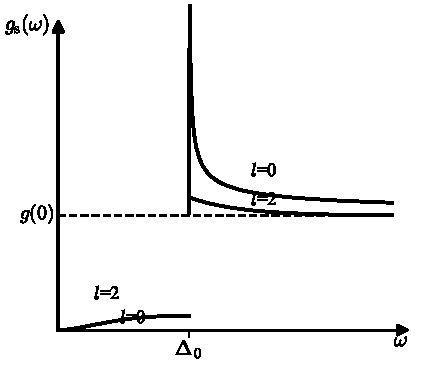
\includegraphics[width=7cm]{fig7-10.pdf}\\{\small 图 7.10\quad s波（$l=0$）与d波（$l=2$）超导体的准粒子态密度}
\end{minipage}
\end{center}

正常金属态密度 $\left[g(0)\right]$ 的趋势.但是，在此低频区域，准粒子的态密度并未消失.这是由于在某些方向上能隙为零，准粒子在节点附近更易于激发，并表现为只要 $\left|\omega\right|>0$ 总存在有限的准粒子态密度，导致在各向异性超导体的准粒子激发谱中不存在真正的能隙.换句话说，与BCS的s波超导体的最明显差别是在 $\left|\omega\right|\ll\Delta_{0}$ 的低频区内仍存在有限的准粒子态密度.

瓦尔玛（Varma）\textsuperscript{[26]}在定性分析了重费密子超导体的低温特性基础上，首先总结出各向异性超导体的低频准粒子态密度 $g_{\mathrm{s}}\sim\left|\omega\right|^{\alpha}$，其中 $\alpha=1$ 代表能隙函数在费密面上具有零线的极向态，$\alpha=2$ 则对应于费密面上存在能隙函数节点的轴向态.显然，图7.10中的d波 $\left(l=2\right)$ 曲线属于轴向态，其低频区态密度正比于 $\omega^{2}$，符合瓦尔玛的幂次规律.为了加深读者对此规律的理解，我们将对p波 $\left(l=1\right)$ 的极向态与轴向态中准粒子的低频态密度作计算：

(i)p波极向态

$\left|\Delta(\hat{\boldsymbol{k}})\right|=\Delta_{0}\left|\cos\theta_{\boldsymbol{k}}\right|$，其中 $\Delta_{0}=\sqrt{3}\,\Delta_{\mathrm{a}}$ 代表最大能隙值（沿 $\theta_{\boldsymbol{k}}=0,\pi$ 方向），在这里赤道线 $\left(\theta_{\boldsymbol{k}}=\dfrac{\pi}{2}\right)$ 为能隙函数的零线，根据式(7.5.4)
\begin{equation*}
  g_{\mathrm{s}}^{\mathrm{polar}}(\omega)=g(0)\frac{\left|\omega\right|}{2}\,\mathrm{Re}
  \int_{-1}^{+1}\mathrm{d}\cos\theta_{\boldsymbol{k}}\,
  \frac{1}{\sqrt{\omega^{2}-\Delta_{0}^{2}\cos^{2}\theta_{\boldsymbol{k}}}}
\end{equation*}
\begin{equation}
\begin{aligned}
  &=\begin{cases}
    g(0)\dfrac{\left|\omega\right|}{2\Delta_{0}}\displaystyle\int_{-1}^{1}\frac{\mathrm{d}x}
    {\sqrt{\left(\dfrac{\omega}{\Delta_{0}}\right)^{2}-x^{2}}} & \left(\left|\omega\right|>\Delta_{0}\right)\\[2em]
    g(0)\dfrac{\left|\omega\right|}{2\Delta_{0}}\,\mathrm{Re}\left[\frac{1}{\mathrm{i}}\int_{-1}^{1}\frac{\mathrm{d}x}
    {\sqrt{x^{2}-\left(\dfrac{\omega}{\Delta_{0}}\right)^{2}}}\right] & \left(\left|\omega\right|<\Delta_{0}\right)
  \end{cases}\\
  &=\begin{cases}
    g(0) & \left(\text{当}\ \left|\omega\right|\gg\Delta_{0}\ \text{时}\right)\\[0.5em]
    g(0)\dfrac{\pi}{2}\cdot\dfrac{\left|\omega\right|}{\Delta_{0}} & \left(\text{当}\ \left|\omega\right|\ll\Delta_{0}\ \text{时}\right)
  \end{cases}
\end{aligned}
\end{equation}
对于“电子型”的准粒子激发，其低频态密度正比于 $\omega$，与瓦尔玛规律一致.在§6中我们还将证明高温超导体的 $d_{x^{2}-y^{2}}$ 配对态也属于存在零线的d波类极向态，其低频态密度也是 $\omega$ 的线性函数.

\subsection*{(ii)p波轴向态}

$\left|\Delta(\hat{\boldsymbol{k}})\right|=\Delta_{0}\left|\sin\theta_{\boldsymbol{k}}\right|$，其中最大能隙值 $\Delta_{0}=\sqrt{\dfrac{3}{2}}\,\Delta_{\mathrm{a}}$，能隙函数的节点在南、北极 $\left(\theta_{\boldsymbol{k}}=0,\pi\right)$ 方向，这时式(7.5.4)可简化为
\begin{equation}
\begin{aligned}
  g_{\mathrm{s}}^{\mathrm{axial}}(\omega)&=g(0)\frac{\left|\omega\right|}{2}\,\mathrm{Re}
  \int_{-1}^{+1}\mathrm{d}\cos\theta_{\boldsymbol{k}}\,
  \frac{1}{\sqrt{\omega^{2}-\Delta_{0}^{2}\sin^{2}\theta_{\boldsymbol{k}}}}\\
  &=g(0)\frac{\left|\omega\right|}{2\Delta_{0}}\ln\left|\frac{\omega+\Delta_{0}}{\omega-\Delta_{0}}\right|\\
  &=\begin{cases}
    g(0) & \left(\text{当}\ \left|\omega\right|\gg\Delta_{0}\ \text{时}\right)\\[0.5em]
    g(0)\left(\dfrac{\omega}{\Delta_{0}}\right)^{2} & \left(\text{当}\ \left|\omega\right|\ll\Delta_{0}\ \text{时}\right)
  \end{cases}
\end{aligned}
\end{equation}
显然，其低频态密度正比于 $\omega^{2}$，也符合瓦尔玛规律.

在各向异性超导体的准粒子态密度曲线中不存在真正的能隙，而是服从 $g_{\mathrm{s}}\left(\left|\omega\right|\ll\Delta_{0}\right)\sim\left|\omega\right|^{\alpha}$（$\alpha=1,2$）的幂次律，这将对其低温超导特征产生重要的影响.

\subsection*{2. 重费密子超导体的低温特性}

在BCS超导体中，由于其态密度曲线中存在能隙，$g_{\mathrm{s}}\left(\left|\omega\right|<\Delta_{0}\right)=0$，$T\ll T_{\mathrm{c}}$ 时的超导准粒子激发应正比于 $\mathrm{e}^{-\beta\Delta_{0}}$，其中 $\Delta_{0}$ 代表零温隙，$\beta=\left(1/k_{\mathrm{B}}T\right)$.因此，在BCS超导体中，一切与准粒子激发有关的物理量，如超导态的低温比热容 $c_{\mathrm{es}}\left(T\ll T_{\mathrm{c}}\right)$［见式(6.5.43)］、穿透深度随温度的变化 $\Delta\lambda\left(T\ll T_{\mathrm{c}}\right)\equiv\lambda(T)-\lambda(0)$［见式(6.8.52)］、低温热导和超声吸收以及反映费密面附近超导准粒子与核磁矩散射的低温核自旋-点阵弛豫率 $T_{1\mathrm{s}}^{-1}\left(T\ll T_{\mathrm{c}}\right)$ 等均已被证实是正比于 $\mathrm{e}^{-\beta\Delta_{0}}$ 的.BCS超导态在 $T\ll T_{\mathrm{c}}$ 时具有指数型的热激发特征标志着这类超导体在费密面上存在着各向同性的能隙.

20世纪80年代初期，在含有稀土（Ce）或锕系（U）元素的金属间化合物中，发现了重费密子系统.这是一种在低温下的重电子（有效质量 $m^{*}=10^{2}\sim10^{3}m_{\mathrm{e}}$）金属材料，实验测出的低温比热容系数 $\gamma$ 和自旋磁化率都比正常金属高2～3个量级.对于重费密子系统的实验研究，展现出十分丰富的物理内容，特别是在这类含磁性离子（如 Ce 与 U）的材料中发现了重费密子超导体.重费密子超导体具有奇异特性，表现为在 $T\ll T_{\mathrm{c}}$ 时的比热容 $c_{\mathrm{es}}(T)$、核自旋-点阵弛豫率 $T_{1\mathrm{s}}^{-1}(T)$、超导与正常态的超声吸收系数比 $\left(\alpha_{\mathrm{S}}/\alpha_{\mathrm{N}}\right)$ 以及伦敦穿透深度随温度的改变等物理量不服从传统BCS超导体的指数型热激发特征 $\mathrm{e}^{-\beta\Delta_{0}}$，而具有温度的简单幂次特征 $T^{n}$，与非声子机制的各向异性的d波配对超导体相类似，具体的实验数值可参看表7.6\textsuperscript{[27,28]}.

表7.6\quad $T\ll T_{\mathrm{c}}$ 时重费密子超导体的特征

\begin{center}\scriptsize
\begin{tabular}{lcccccc}
\hline
重费密子低温 & $\mathrm{CeCu}_{2}\mathrm{Si}_{2}$ & $\mathrm{UBe}_{13}$ & $\mathrm{UPt}_{3}$ & BCS & d波极向态 & d波轴向态\\
超导体特性 & $\left(T_{\mathrm{c}}=0.7\ \mathrm{K}\right)$ & $\left(T_{\mathrm{c}}=1\ \mathrm{K}\right)$ & $\left(T_{\mathrm{c}}=0.5\ \mathrm{K}\right)$ & 超导体 & & \\
\hline
$c_{\mathrm{es}}\left(T\ll T_{\mathrm{c}}\right)$ & $\sim T^{2.8}$ & $\sim T^{2.86}$ & $\sim T^{2}$ & $\sim\mathrm{e}^{-\Delta_{0}/k_{\mathrm{B}}T}$ & $\sim T^{2}$ & $\sim T^{3}$\\
$T_{1\mathrm{s}}^{-1}\left(T\ll T_{\mathrm{c}}\right)$ & $\sim T^{3}$（$^{63}$Cu） & $\sim T^{3}$（$^{9}$Be） & $\sim T^{3}$（$^{195}$Pt） & $\sim T\mathrm{e}^{-\Delta_{0}/k_{\mathrm{B}}T}$ & $\sim T^{3}$ & $\sim T^{5}$\\
$\alpha_{\mathrm{S}}/\alpha_{\mathrm{N}}$ & $?$ & $\sim T^{2}$ & $\sim T^{2}$ & $\sim\mathrm{e}^{-\Delta_{0}/k_{\mathrm{B}}T}$ & $\sim T^{2}$ & $\sim T^{4}$\\
$\Delta\lambda\left(T\ll T_{\mathrm{c}}\right)$ & $\sim T^{2}$ & $\sim T^{2}$ & $\sim T^{2}$ & $\sim\mathrm{e}^{-\Delta_{0}/k_{\mathrm{B}}T}$ &
$\begin{cases}T\left(\mbox{纯}\right)\\ T^{2}\left(\mbox{含杂}\right)\end{cases}$ & $\sim T^{2}$\\
\hline
\end{tabular}
\end{center}

{\emergencystretch 3em
表中的低温比热容和核弛豫率可根据固体物理公式：$c_{\mathrm{es}}\left(T\ll T_{\mathrm{c}}\right)\sim\allowbreak g_{\mathrm{s}}\left(\left|\omega\right|=k_{\mathrm{B}}T\right)\cdot T$ 和 $T_{1\mathrm{s}}^{-1}\left(T\ll T_{\mathrm{c}}\right)\sim\allowbreak g_{\mathrm{s}}\left(\left|\omega\right|=k_{\mathrm{B}}T\right)c_{\mathrm{es}}\left(T\right)$ 作定性估计，其中极向态与轴向态的超导态密度分别正比于 $\omega$ 与 $\omega^{2}$.\par}

仔细分析表7.6中各种重费密子超导体的特征可以看出：$\mathrm{UPt}_{3}$ 基本符合极向态特征，只需假定由于杂质的共振散射效应使极向态的 $\Delta\lambda\left(T\right)$ 正比于 $T^{2}$.至于其它两种重费密子超导体，目前的实验结果还很难断定它们是极向态还是轴向态，尽管较多的数据显示为极向态.在配对的对称性方面，群表示论的研究已证明对于具有立方 $\left(\mathrm{UBe}_{13}\right)$、四角 $\left(\mathrm{CeCu}_{2}\mathrm{Si}_{2}\right)$ 和六角 $\left(\mathrm{UPt}_{3}\right)$ 晶系结构的晶体，在考虑了强自旋-轨道耦合效应后，不存在自旋为三重态配对的p波 $\left(l=1\right)$ 极向态，只可能有自旋单重态配对的d波 $\left(l=2\right)$ 极向态，当然也存在d波轴向态，正是在这个意义上，人们倾向于重费密子超导体是d波超导体.至于是有零线的d波极向态，还是只有节点（零点）的d波轴向态，目前尚难于鉴别，还需要更直接的实验证据.但是，根据重费密子超导体的低温热力学与输运特性服从 $T^{n}$ 幂次律（而不是BCS的指数型 $\mathrm{e}^{-\beta\Delta_{0}}$ 激发规律）的共同特点，至少可以断言：实验表明重费密子超导体是具有非零角动量 $\left(l>0\right)$ 的各向异性超导体.

\section{高温超导体的异常低温特性}

在本章§3中已经指出，铜氧化物高温超导体具有不同于BCS超导体的低温特性，在本节中我们将利用各向异性超导理论，具体求出 $d_{x^{2}-y^{2}}$ 波配对的超导体中低能区准粒子态密度，用于计算 $T\ll T_{\mathrm{c}}$ 时超导态的比热容、伦敦穿透深度和核自旋-点阵弛豫率，并证实在表7.4中所列出的异常低温特性是与 $d_{x^{2}-y^{2}}$ 波配对特征一致的.

\subsection*{1. $d_{x^{2}-y^{2}}$ 波的低频准粒子态密度}

可以将角分辨光电子发射谱（简称ARPES）等实验所证实的 $d_{x^{2}-y^{2}}$ 波能隙函数式(7.3.1)具体写为
\begin{equation}
  \Delta(\hat{\boldsymbol{k}})=\Delta_{0}\cos2\phi\,,\qquad
  \phi=\arctan\left(\hat{k}_{y}/\hat{k}_{x}\right)
\end{equation}
其中 $\hat{k}_{x}$ 与 $\hat{k}_{y}$ 是在平行于 $\mathrm{CuO}_{2}$ 平面的二维BZ中的单位波矢 $\hat{\boldsymbol{k}}$（$\left|\hat{\boldsymbol{k}}\right|=1$）沿x与y轴的分量，$\Delta_{0}$ 代表最大能隙值，而相角 $\phi$ 则从 $k_{x}$ 轴计算.系统在 $d_{x^{2}-y^{2}}$ 波态的超导准粒子态密度可利用式(7.5.4)作计算.将式(7.6.1)代入该式，不难写出在 $0<\omega<\Delta_{0}$ 区域中的态密度为
\begin{equation}
\begin{aligned}
  g_{\mathrm{s}}\left(\omega<\Delta_{0}\right)
  &=g(0)\,\mathrm{Re}\int_{0}^{2\pi}\left(\frac{\mathrm{d}\phi}{2\pi}\right)
  \frac{\omega}{\sqrt{\omega^{2}-\Delta_{0}^{2}\cos^{2}(2\phi)}}\\
  &=g(0)\frac{\left|\omega\right|}{\sqrt{\Delta_{0}^{2}-\omega^{2}}}\left(\frac{2}{\pi}\right)\times\\
  &\quad\mathrm{Re}\int_{0}^{\pi/2}\frac{\mathrm{d}\left(2\phi\right)}
  {\sqrt{\left(\dfrac{\Delta_{0}^{2}}{\Delta_{0}^{2}-\omega^{2}}\right)\sin^{2}(2\phi)-1}}
\end{aligned}
\end{equation}
当 $\omega\ll\Delta_{0}$ 时，可将低频区的态密度近似写为
\begin{equation}
  g_{\mathrm{s}}\left(\omega\ll\Delta_{0}\right)=g(0)\left(\frac{\omega}{\Delta_{0}}\right)\cdot\left(\frac{2}{\pi}\right)\cdot
  \mathrm{Re}\int_{0}^{2\pi}\frac{\mathrm{d}\left(2\phi\right)}{\sqrt{\sin^{2}(2\phi)-1}}
\end{equation}
作变量代换 $2\phi=\mathrm{i}x$，这时 $\sin^{2}(2\phi)=-\sinh^{2}x$，从而得到
\begin{equation}
  g_{\mathrm{s}}\left(\omega\ll\Delta_{0}\right)\approx g(0)\left(\frac{\omega}{\Delta_{0}}\right)\cdot\left(\frac{2}{\pi}\right)\cdot
  \mathrm{Re}\int_{0}^{2\pi}\mathrm{sech}\,x\,\mathrm{d}x\approx g(0)\left(\frac{\omega}{\Delta_{0}}\right)\sim\omega
\end{equation}
在上式中只需取积分的实部，它恰好等于 $\pi/2$.这样就求出了 $d_{x^{2}-y^{2}}$ 波的低频态密度正比于 $\omega$，这个结果与§5中所证明的在三维费密面上存在能隙的零线情况（即极向态）是一致的.在这里我们要提醒读者注意，式(7.6.1)所给出的能隙函数 $\Delta(\hat{\boldsymbol{k}})=\Delta\left(\hat{k}_{x},\hat{k}_{y}\right)$ 是与垂直于 $\mathrm{CuO}_{2}$ 平面方向的动量 $\hat{k}_{z}$ 无关的，这是高温超导铜氧化合物的层状结构所导致的准二维特征.由于相同的原因，系统的三维费密面也具有准二维特征.实际上，能带计算同样表明沿 $k_{z}$ 方向的能带色散可以忽略.因此，系统的三维费密面可以简单看作是二维费密面沿 $k_{z}$ 方向的无色散延伸所构成的柱面.这时，在 $k_{x}$ 与 $k_{y}$ 平面内二维费密面沿 $k_{x}=\pm k_{y}$ 方向的节点在三维动量空间中将构成平行于 $k_{z}$ 方向的零线.因此式(7.6.1)所给出的 $d_{x^{2}-y^{2}}$ 波能隙函数属于在三维费密面上存在零线的d波极向态，其低频准粒子态密度自然具有 $\omega$ 的线性激发特征，并由式(7.6.4)描述.下面将利用此态密度计算氧化物高温超导体的低温物性.

\subsection*{2. $d_{x^{2}-y^{2}}$ 波超导态的低温特性}

低温比热容：从式(6.5.39)出发，类似于s波BCS超导体的低温比热容计算，在 $T\ll T_{\mathrm{c}}$ 时略去该式中 $\beta\left(\mathrm{d}\Delta^{2}/\mathrm{d}\beta\right)$ 项，求得
\begin{equation}
\begin{aligned}
  c_{\mathrm{s}}&\approx2\beta k_{\mathrm{B}}\sum_{k}\hat{\xi}_{k}^{2}
  \left[-\frac{\partial f\left(\hat{\xi}_{k}\right)}{\partial\hat{\xi}_{k}}\right]\\
  &\approx4\beta k_{\mathrm{B}}g(0)\int_{0}^{\infty}\mathrm{d}\varepsilon\,\hat{\xi}^{2}
  \left[-\frac{\partial f(\hat{\xi})}{\partial\hat{\xi}}\right]
  \qquad\left(T\ll T_{\mathrm{c}}\right)
\end{aligned}
\end{equation}
{\emergencystretch 3em
利用在费密面附近正常态与超导态态密度的关系 $g(0)\,\mathrm{d}\varepsilon=\allowbreak g_{\mathrm{s}}(\hat{\xi})\,\mathrm{d}\hat{\xi}$ 以及 $\left[-\partial f/\partial\hat{\xi}\right]=\allowbreak\beta\mathrm{e}^{\beta\hat{\xi}}/\left(\mathrm{e}^{\beta\hat{\xi}}+1\right)^{2}$，可将上式写成\par}
\begin{equation}
\begin{aligned}
  c_{\mathrm{s}}&\approx4\beta^{2}k_{\mathrm{B}}\int_{0}^{\infty}\mathrm{d}\omega\,g_{\mathrm{s}}(\omega)\cdot\omega^{2}\cdot
  \frac{\mathrm{e}^{\beta\omega}}{\left(\mathrm{e}^{\beta\omega}+1\right)^{2}}\\
  &\approx\left(\frac{16k_{\mathrm{B}}}{\beta^{2}\Delta_{0}}\right)\int_{0}^{\infty}\mathrm{d}x\,x^{3}\,\mathrm{sech}^{2}x
  \qquad\left(T\ll T_{\mathrm{c}}\right)
\end{aligned}
\end{equation}
其中 $x=\dfrac{1}{2}\beta\omega$，再利用积分公式 $\int_{0}^{\infty}\mathrm{d}x\,x^{3}\,\mathrm{sech}^{2}x=\left(9/8\right)\zeta(3)$，可求出低温比热容
\begin{equation}
  c_{\mathrm{s}}\left(T\ll T_{\mathrm{c}}\right)\approx18\zeta(3)\left[\frac{g(0)}{\Delta_{0}}\right]k_{\mathrm{B}}^{3}T^{2}\sim T^{2}
\end{equation}
此结果与实验测量一致.若引入线性比热容系数 $\gamma_{\mathrm{s}}(T)\equiv c_{\mathrm{s}}(T)/T$，则求得 $\gamma_{\mathrm{s}}(T)\sim g_{\mathrm{s}}\left(\left|\omega\right|=k_{\mathrm{B}}T\right)\sim T$，可导出表7.6中所用的固体物理学公式 $c_{\mathrm{s}}\left(T\ll T_{\mathrm{c}}\right)\sim g_{\mathrm{s}}\left(\left|\omega\right|=k_{\mathrm{B}}T\right)\cdot T$，这是利用低频区准粒子态密度定性估计低温比热容与温度关系的一个有用公式.

伦敦穿透深度：从式(6.8.50)出发
\begin{equation*}
  \left[\frac{\lambda_{\mathrm{L}}(0)}{\lambda_{\mathrm{L}}(T)}\right]^{2}
  =1-2\beta\int_{0}^{\infty}\mathrm{d}\omega
  \left[\frac{g_{\mathrm{s}}(\omega)}{g(0)}\right]f(\omega)\left[1-f(\omega)\right]
\end{equation*}
考虑到 $T\ll T_{\mathrm{c}}$ 时，$\left[\lambda_{\mathrm{L}}(0)/\lambda_{\mathrm{L}}(T)\right]^{2}-1\approx2\left[\lambda_{\mathrm{L}}(0)-\lambda_{\mathrm{L}}(T)\right]/\lambda_{\mathrm{L}}(0)=-2\Delta\lambda/\lambda_{\mathrm{L}}(0)$，可得到伦敦穿透深度的变化为
\begin{equation}
  \frac{\Delta\lambda\left(T\ll T_{\mathrm{c}}\right)}{\lambda_{\mathrm{L}}(0)}
  \approx\beta\int_{0}^{\infty}\mathrm{d}\omega\,\frac{g_{\mathrm{s}}(\omega)}{g(0)}f(\omega)\left[1-f(\omega)\right]
\end{equation}
将 $d_{x^{2}-y^{2}}$ 波的低频准粒子态密度公式(7.6.4)代入上式，立刻求得
\begin{equation}
\begin{aligned}
  \frac{\Delta\lambda\left(T\ll T_{\mathrm{c}}\right)}{\lambda_{\mathrm{L}}(0)}
  &\approx\beta\int_{0}^{\infty}\mathrm{d}\omega\left(\frac{\omega}{\Delta_{0}}\right)
  \frac{\mathrm{e}^{\beta\omega}}{\left(\mathrm{e}^{\beta\omega}+1\right)^{2}}
  =\left(\frac{k_{\mathrm{B}}T}{\Delta_{0}}\right)\int_{0}^{\infty}\mathrm{d}x\,x\,\mathrm{sech}^{2}x\\
  &=\left(\frac{k_{\mathrm{B}}T}{\Delta_{0}}\right)\ln2\sim T
\end{aligned}
\end{equation}
显然与表7.4中 $\Delta\lambda\left(T\ll T_{\mathrm{c}}\right)\sim T$ 的实验结果一致，说明高温超导体属于 $d_{x^{2}-y^{2}}$ 波配对的超导态.最后再看 $T_{1\mathrm{s}}^{-1}$ 的计算结果：

核自旋-点阵弛豫率：可直接利用固体物理的定性公式，由低频态密度与低温比热容求出
\begin{equation}
  T_{1\mathrm{s}}^{-1}\left(T\ll T_{\mathrm{c}}\right)\sim g_{\mathrm{s}}\left(\left|\omega\right|=k_{\mathrm{B}}T\right)\cdot c_{\mathrm{s}}\left(T\ll T_{\mathrm{c}}\right)\sim T^{3}
\end{equation}
它也与表7.4中所列出的测量结果定性相符.

总之，在铜氧化合物高温超导体中，$T\ll T_{\mathrm{c}}$ 时超导态中物理特性的实验结果与ARPES和SQUID等方法确定的 $d_{x^{2}-y^{2}}$ 波超导态特征是相吻合的，进一步证实了这类超导体是能隙函数存在零线的d波各向异性配对超导体.高温超导体在配对对称性的研究方面已经比较早发现的重费密子超导体更为深入和确定了.

\subsection*{3. $d_{x^{2}-y^{2}}$ 波超导态的零温能隙与$T_{\mathrm{c}}$之比值}

从各向异性超导体的有限温度能隙方程式(7.4.28)出发，取 $d_{x^{2}-y^{2}}$ 波的二维超导能隙函数公式(7.6.1)
\begin{equation*}
  \Delta\left(\hat{\boldsymbol{k}},T\right)=\Delta_{0}(T)\cos2\phi\,,\qquad
  \phi=\arctan\left(\hat{k}_{y}/\hat{k}_{x}\right)
\end{equation*}
相应的在二维平面中的吸引势取为
\begin{equation}
  V\left(\hat{\boldsymbol{k}}\cdot\hat{\boldsymbol{k}}'\right)=-V_{\mathrm{d}}\cos\left[2\left(\phi-\phi'\right)\right]
  \qquad\left(V_{\mathrm{d}}>0\right)
\end{equation}
这时 $d_{x^{2}-y^{2}}$ 波的二维能隙方程变为
\begin{equation*}
\begin{aligned}
  \Delta_{0}(T)\cos(2\phi)
  &=V_{\mathrm{d}}\cos(2\phi)\sum_{k'}
  \frac{\cos^{2}(2\phi')\tanh\left(\dfrac{1}{2}\beta\hat{\xi}_{k'}\right)}{2\hat{\xi}_{k'}}\\
  &\quad+V_{\mathrm{d}}\sin(2\phi)\sum_{k'}
  \frac{\cos(2\phi')\sin(2\phi')\tanh\left(\dfrac{1}{2}\beta\hat{\xi}_{k'}\right)}{2\hat{\xi}_{k'}}
\end{aligned}
\end{equation*}
其中
\begin{equation}
  \hat{\xi}_{k'}\equiv\left[\varepsilon_{k'}^{2}+\left|\Delta_{0}(T)\cos(2\phi')\right|^{2}\right]^{1/2}
\end{equation}
由于在二维能隙方程的等式右边第二项是 $\phi'$ 的奇函数，当对 $\hat{\boldsymbol{k}}'$ 作求和时此项应为零，从而可求得与式(7.4.30a)相应的 $d_{x^{2}-y^{2}}$ 波自洽方程：
\begin{equation}
  1=V_{\mathrm{d}}\sum_{k'}\frac{\cos^{2}(2\phi')\tanh\left(\dfrac{1}{2}\beta\hat{\xi}_{k'}\right)}{2\hat{\xi}_{k'}}
\end{equation}
由此可具体计算 $\Delta_{0}(0)$ 与 $T_{\mathrm{c}}$.

零温能隙：
\begin{equation*}
\begin{aligned}
  1&=\frac{1}{2}V_{\mathrm{d}}\sum_{k'}
  \frac{\cos^{2}(2\phi')}{\sqrt{\varepsilon_{k'}^{2}+\Delta_{0}^{2}(0)\cos^{2}(2\phi')}}\\
  &=\frac{1}{2}g(0)V_{\mathrm{d}}\int_{0}^{2\pi}\frac{\mathrm{d}\phi}{2\pi}
  \int_{-\hbar\omega_{0}}^{\hbar\omega_{0}}\mathrm{d}\varepsilon\,
  \frac{\cos^{2}(2\phi)}{\sqrt{\varepsilon^{2}+\Delta_{0}^{2}(0)\cos^{2}(2\phi)}}\\
  &=g(0)V_{\mathrm{d}}\int_{0}^{2\pi}\frac{\mathrm{d}\phi}{2\pi}\cos^{2}(2\phi)
  \ln\left[\frac{2\hbar\omega_{0}}{\Delta_{0}(0)\left|\cos(2\phi)\right|}\right]
\end{aligned}
\end{equation*}
其中考虑了弱耦合超导理论中的近似条件 $\Delta_{0}(T)\ll\hbar\omega_{0}$，因此零温时最大能隙 $\Delta_{0}(0)$ 满足方程
\begin{equation*}
  1=\frac{1}{2}g(0)V_{\mathrm{d}}\ln\left[2\Gamma\hbar\omega_{0}/\Delta_{0}(0)\right]
\end{equation*}
由此求出
\begin{equation*}
  \Delta_{0}(0)=\left(2\hbar\omega_{0}\right)\Gamma\exp\left[\frac{-1}{\dfrac{1}{2}g(0)V_{\mathrm{d}}}\right]
\end{equation*}
其中
\begin{equation*}
\begin{aligned}
  \ln\Gamma&\equiv-\left(\frac{4}{\pi}\right)\int_{0}^{\pi/2}\mathrm{d}\left(2\phi\right)\cos^{2}(2\phi)\ln\cos(2\phi)\\
  &=-\left(4/\pi\right)\int_{0}^{1}\mathrm{d}x\,x^{2}\ln x/\sqrt{1-x^{2}}=\ln\left(\frac{2}{\sqrt{\mathrm{e}}}\right)
\end{aligned}
\end{equation*}
在这里 $x\equiv\cos(2\phi)$，零温时 $d_{x^{2}-y^{2}}$ 波的最大能隙为
\begin{equation}
\begin{aligned}
  &\Delta_{0}(0)=\Gamma\cdot\left(2\hbar\omega_{0}\right)\exp\left[\frac{-1}{\dfrac{1}{2}g(0)V_{\mathrm{d}}}\right]\\
  &\Gamma=2/\sqrt{\mathrm{e}}>1
\end{aligned}
\end{equation}
至于在零温时 $d_{x^{2}-y^{2}}$ 波的平均能隙 $\Delta_{\mathrm{a}}(0)$，根据式(7.4.37)与(7.4.38)，应满足条件：
\begin{equation}
  \Delta_{\mathrm{a}}^{2}(0)=\int_{0}^{2\pi}\frac{\mathrm{d}\phi}{2\pi}\Delta_{0}^{2}(0)\cos^{2}(2\phi)
  =\frac{1}{2}\Delta_{0}^{2}(0)
\end{equation}
因此 $\Delta_{\mathrm{a}}(0)=\Delta_{0}(0)/\sqrt{2}$，其解析表示式为
\begin{equation}
\begin{aligned}
  &\Delta_{\mathrm{a}}(0)=Q\cdot\left(2\hbar\omega_{0}\right)\exp\left[\frac{-1}{\dfrac{1}{2}g(0)V_{\mathrm{d}}}\right]\\
  &Q=\sqrt{\left(2/\mathrm{e}\right)}<1
\end{aligned}
\end{equation}
与式(7.4.44)所给出的一般性结论 $Q<1$ 相符合.

转变温度 $T_{\mathrm{c}}$：可从有限温度的自洽方程式(7.6.13)出发，考虑到 $T=T_{\mathrm{c}}$ 时能隙 $\Delta_{0}\left(T_{\mathrm{c}}\right)=0$，求出
\begin{equation*}
\begin{aligned}
  1&=g(0)V_{\mathrm{d}}\left[\int_{0}^{2\pi}\frac{\mathrm{d}\phi}{2\pi}\cos^{2}(2\phi)\right]
  \int_{0}^{\hbar\omega_{0}}\mathrm{d}\varepsilon\,\frac{\tanh\left(\varepsilon/2k_{\mathrm{B}}T_{\mathrm{c}}\right)}{\varepsilon}\\
  &=\frac{1}{2}g(0)V_{\mathrm{d}}\ln\left[\left(\frac{2\mathrm{e}^{\gamma}}{\pi}\right)\left(\frac{\hbar\omega_{0}}{k_{\mathrm{B}}T_{\mathrm{c}}}\right)\right]
\end{aligned}
\end{equation*}
因此
\begin{equation}
  k_{\mathrm{B}}T_{\mathrm{c}}=\left(2\mathrm{e}^{\gamma}/\pi\right)\hbar\omega_{0}\exp\left[\frac{-1}{\dfrac{1}{2}g(0)V_{\mathrm{d}}}\right]
\end{equation}
由此求得在弱耦合情形 $d_{x^{2}-y^{2}}$ 波配对的零温最大能隙与 $T_{\mathrm{c}}$ 之比值为
\begin{equation}
  \left[2\Delta_{0}(0)/k_{\mathrm{B}}T_{\mathrm{c}}\right]=\left(2\pi\mathrm{e}^{-\gamma}\right)\Gamma=4.28
  \qquad\left(\Gamma=2/\sqrt{\mathrm{e}}>1\right)
\end{equation}
它略大于BCS弱耦合超导体的标准值3.53，但是弱耦合 $d_{x^{2}-y^{2}}$ 波的零温平均能隙 $\Delta_{\mathrm{a}}(0)$ 与 $T_{\mathrm{c}}$ 之比值则为
\begin{equation}
  \left[2\Delta_{\mathrm{a}}(0)/k_{\mathrm{B}}T_{\mathrm{c}}\right]=\left(2\pi\mathrm{e}^{-\gamma}\right)Q=3.03
  \qquad\left(Q=\sqrt{2/\mathrm{e}}<1\right)
\end{equation}
它总是小于3.53，与式(7.4.45)一致.以上两个特征性比值都可以用作判断铜氧化合物高温超导体是否属于弱耦合情形.早期的实验测量多半是用陶瓷或多晶样品，所测得的比值应代表平均能隙 $2\Delta_{\mathrm{a}}(0)$ 与 $k_{\mathrm{B}}T_{\mathrm{c}}$ 之比，其实测值往往大于5.近年来由于实验技术的发展，已能在良好制备的单晶中较准确的测量最大能隙 $\Delta_{0}$，实验给出的 $2\Delta_{0}(0)$ 与 $T_{\mathrm{c}}$ 之比值在8～9之间，也明显超出了式(7.6.18)所规定的范围.因此，无论从最大能隙或者从平均能隙与 $T_{\mathrm{c}}$ 之比值的实验结果来判断，高温超导体都不能用弱耦合描述，而必须采用强耦合的超导理论.

\section{高温超导体正常态的反常特征（最佳化合物）}

众所周知，在电声子机制的BCS超导体中，$T>T_{\mathrm{c}}$ 时的正常态是普通的金属态，并且完全可以用标准的朗道费密液体理论描述.正由于对费密液体有比较深入的了解，BCS等人从费密面附近一对动量和自旋取向相反的电子间通过声子传递有效的吸引作用可以导致费密球态失稳的特征，提出了常规超导体中配对吸引来源于电子与声子的相互作用，简称配对的声子机制.因此，为了探明形成超导的微观机制，必须对 $T>T_{\mathrm{c}}$ 正常态的特性有比较清楚的了解.人们自然会问，在铜氧化合物中 $T>T_{\mathrm{c}}$ 时的金属性正常态是否仍然属于费密液体？大量的实验结果表明其正常态的许多物理性质，例如 $T>T_{\mathrm{c}}$ 时的直流电阻率、光电导以及核磁共振（NMR）中的自旋-点阵弛豫率等，均与普通金属行为很不相同，表现出十分异常的奇特行为，而且均不能用标准的朗道费密液体理论描述，这就是人们通常所说的高温超导体正常态的反常特征.限于篇幅，我们仅选择几个主要的实验事实来说明其正常态的反常，详细的讨论可参考文献\textsuperscript{[29]}.在本节中我们主要介绍最佳化合物正常态的非费密液体行为，而在下节中再介绍在弱掺杂区中新近发现的正常态能隙等奇异现象.

早期对正常态特征的研究多集中于讨论具有最高超导转变温度 $T_{\mathrm{c}}=T_{\mathrm{c}}^{\mathrm{max}}$ 的最佳化合物，如 $\mathrm{La}_{2-x}\mathrm{Sr}_{x}\mathrm{CuO}_{4}$（$x\approx0.15$）及 $\mathrm{YBa}_{2}\mathrm{Cu}_{3}\mathrm{O}_{6+x}$（$x\approx1$）等的输运性质及核磁共振谱的反常.高温超导体正常态最为突出的反常特征是在最简单的直流电阻率 $\rho_{\mathrm{ab}}$ 的测量中被发现的，这里的 $\rho_{\mathrm{ab}}$ 代表沿导电层（即 $\mathrm{CuO}_{2}$ 平面）方向的正常态电阻率.对于所有的铜氧化合物高温超导体，在最佳掺杂（即最佳化合物）情况下，正常态的一个重要反常特征是

\subsection*{1. $\rho_{\mathrm{ab}}$普遍地具有线性温度行为}

大量的实验报道证实，所有最佳化合物沿导电层的直流电阻率均随温度升高而线性增大，其线性温区可从下界温度 $T_{\mathrm{c}}$ 一直延伸到很高的上界温度 $T_{\mathrm{max}}$.对于 $x=0.15$ 的掺杂（Sr）La-214 系统，$T_{\mathrm{max}}=1\,000$ K，而Y-123 和 Bi-2212 最佳化合物也可以延伸到600 K.特别值得指出的是，Bi-2201（$\mathrm{Bi}_{2}\mathrm{Sr}_{2}\mathrm{CuO}_{6}$）由于 $T_{\mathrm{c}}$（约为7 K）很低，其 $\rho_{\mathrm{ab}}$ 的线性温度关系在7～700 K的宽阔温区内都成立.线性温区的下界温度可以低于10 K是正常态电阻率反常的一个重要特点.

最佳化合物的正常态 $\rho_{\mathrm{ab}}$ 可用下列公式描述：
\begin{equation}
  \rho_{\mathrm{ab}}(T)=\alpha T+\rho_{0}
\end{equation}
其中 $\alpha$ 是线性温度关系的斜率，$\rho_{0}$ 为将 $\rho_{\mathrm{ab}}(T)$ 的线性关系外延到绝对零度时的插值，也可称为“剩余电阻率”.随着样品质量的不断提高，测出的 $\rho_{0}$ 值越来越小，可以认为，高质量样品的 $\rho_{0}$ 值将趋于零，这时表征 $\rho_{\mathrm{ab}}(T)$ 的物理参数只是 $\alpha$.图7.11中给出了几种高温超导体正常态的 $\rho_{\mathrm{ab}}(T)$ 曲线，其中除了Y-123（60 K）样品外，其它均为最佳化合物，虽然它们的具体结构有很大差异，但它们在 $T_{\mathrm{c}}$ 之上的 $\rho_{\mathrm{ab}}$ 曲线却均具有近似的线性行为，而且 $\alpha$ 的数值也很相近.至于图7.11中的 Y-123（60 K）材料是 $T_{\mathrm{c}}=60$ K 的 $\mathrm{YBa}_{2}\mathrm{Cu}_{3}\mathrm{O}_{6+x}$（$x=0.6\sim0.7$）样品，属于弱（或欠）掺杂的Y-123系统，其 $\rho_{\mathrm{ab}}$ 曲线在 $T_{\mathrm{c}}$ 以上的一段温区内明显地偏离线性规律是由于在正常态中形成了能隙，我们将在§8中再作讨论.

应当明白，在7～1000 K这样广阔的温度范围内，沿导电层的电阻率 $\rho_{\mathrm{ab}}$ 与温度成线性关系是十分异常的现象，它与普通金属的 $\rho$-$T$ 特征判然有别.在普通金属中，电阻率随温度的变化主要来源于电声子散射.熟习固体物理学的读者都知道，来源于电子-声子散射的金属电阻率由布洛赫-格林艾森（Bloch-Grüneisen）公式（以下简称B-G公式）\textsuperscript{[30]}描述，在三维系统中B-G公式可以写为
\begin{equation}
  \rho(T)=A\left(T/\theta_{\mathrm{D}}\right)^{5}\int_{0}^{\theta_{\mathrm{D}}/T}\mathrm{d}z\,
  \frac{z^{5}}{\left(\mathrm{e}^{z}-1\right)\left(1-\mathrm{e}^{-z}\right)}
  \sim\begin{cases}T & \left(T\gg\theta_{\mathrm{D}}\right)\\[0.3em]
  T^{5} & \left(T\ll\theta_{\mathrm{D}}\right)\end{cases}
\end{equation}

\begin{center}
\begin{minipage}{9cm}
\centering
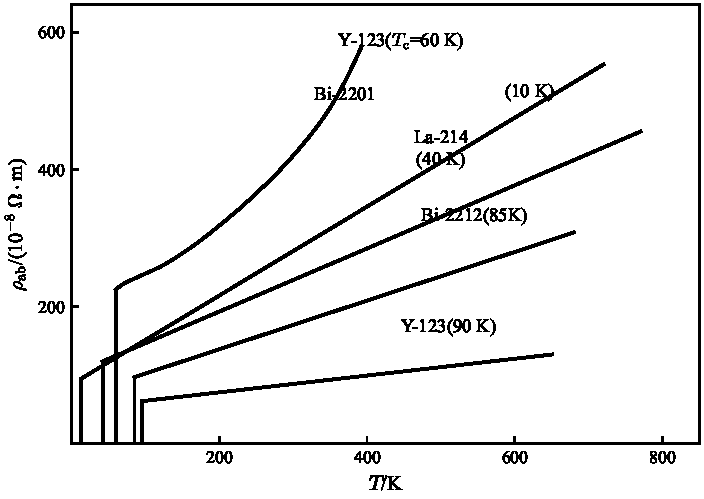
\includegraphics[width=9cm]{fig7-11.pdf}\\{\small 图 7.11\quad 几种高温超导体正常态的 $\rho_{\mathrm{ab}}(T)$ 曲线}
\end{minipage}
\end{center}

其中 $\theta_{\mathrm{D}}$ 是德拜温度，对于普通金属大约在200～400 K之间，而对于铜氧化合物高温超导体 $\theta_{\mathrm{D}}$ 的取值也不低于200 K.B-G公式所预言的在 $T\ll\theta_{\mathrm{D}}$ 低温区 $\rho\sim T^{5}$ 和在室温附近的 $\rho\sim T$ 线性关系是人们早已熟知的定性概念.若进一步对B-G公式作定量的计算，其结果与普通金属中电阻率的测量数据符合良好，如图7.12所示.从图中可以看出，实际上普遍金属电阻率的线性温度区可以放宽到 $T>\left(\theta_{\mathrm{D}}/5\right)$，约在40 K以上，$\left(\theta_{\mathrm{D}}/5\right)$ 可作为线性温区的下界，低于此下界温度应当进入电声子机制电阻率的非线性温度区.但是 Bi-2201 中的线性温度区下界可延续到10 K以下，远低于电声子机制中线性区的下界（40 K），导致在B-G公式的非线性区域中出现反常的线性行为，从而对电声子机制对于铜氧化合物的适用性提出了严重的挑战.此外，在 $T\ll\theta_{\mathrm{D}}$ 的低温区中，迄今尚未观察到在铜氧化物中出现 $\rho\sim T^{5}$（三维）或 $T^{4}$（二维）的行为.这些结果都不能用电子被声子散射来解释.另一方面，在普通金属中还存在电阻率的高温饱和现象，其物理原因是随着温度T的升高，电子与声子的散射效应将不断地增强，导致载流子平均自由程不断地减小，而平均自由程有一个下限，它不能小于近邻原子的间距，此即著名的约飞（Ioffe）判据，这个下限的存在导致电声子散射机制的电阻率在高温时趋向于饱和.文献\textsuperscript{[31]}用 Cu-O 键长作为电子被声子散射平均自由程的下限，定性地估计了铜氧化合物中电声子机制的饱和电阻率约为1 $\mathrm{m\Omega\cdot cm}$，然而在最佳掺杂的 La-214 系统中线性温区可高达1000 K，所对应的 $\rho_{\mathrm{ab}}$ 值早已超过1 $\mathrm{m\Omega\cdot cm}$（如图7.16所示），却未见饱和迹象，这也是电声子机制不能解释的.

\begin{center}
\begin{minipage}{7.5cm}
\centering
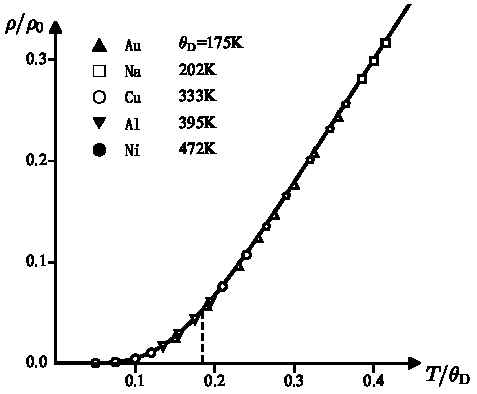
\includegraphics[width=7.5cm]{fig7-12.pdf}\\{\small 图 7.12\quad 几种简单金属的电阻率-温度曲线}\\[0.2em]
{\small （其中实线代表B-G公式的定量计算曲线）}
\end{minipage}
\end{center}

综上所述，正常态电阻率在异常宽的温度范围内满足线性规律实际上已排除了声子作为载流子散射主要来源的可能性，我们有理由认为，在高温超导体正常态中的电阻率反常不是电子-声子散射所造成的.为了解释 $\rho_{\mathrm{ab}}$ 的普适线性温度行为，应当寻找新的散射机制，而探明产生电阻反常的原因，必将有助于解开高温超导电性之谜.历史上在BCS常规超导体中，正是同一种相互作用（电声子耦合）既产生正常态的电阻，又导致在 $T\leqslant T_{\mathrm{c}}$ 时失去电阻和形成超导电性.

此外，在良好制备的Y-123最佳化合物中，从直流电阻率 $\rho_{\mathrm{ab}}(T)$ 的倒数求出的直流（静态）导电率 $\sigma_{\mathrm{ab}}(T)=1/\rho_{\mathrm{ab}}(T)$ 也与从光学（动态）导电率 $\sigma_{\mathrm{ab}}(\omega,T)$ 测量所得到的零频极限 $\sigma_{\mathrm{ab}}(\omega=0,T)$ 值定量相符.这使得人们可以组合两种测量数据，导出一个唯象公式，用于统一描述高温超导体正常态的动态与静态电导特征.

\subsection*{2. 解释光电导率反常的一个唯象公式}

利用光在单晶上垂直入射的反射比 $R(\omega)$ 的测量，可以在很宽的光子能量范围提供金属中动态导电率 $\sigma(\omega)$ 的重要信息.这是因为光的垂直入射的反射比，根据式(2.7.17)，可表示为
\begin{equation}
  R(\omega)=\left|\frac{\sqrt{\varepsilon(\omega)}-1}{\sqrt{\varepsilon(\omega)}+1}\right|^{2}
\end{equation}
其中 $\varepsilon(\omega)$ 是金属的介电函数，而在金属中 $\varepsilon(\omega)$ 与光导电率 $\sigma(\omega)$ 是密切相关的物理量，并且在固体物理学中已经介绍了\textsuperscript{[32]}它们的关系式
\begin{equation}
  \varepsilon(\omega)=1+\mathrm{i}\,4\pi\sigma(\omega)/\omega
\end{equation}
和描述光导电率的特鲁德（Drude）公式
\begin{equation}
  \sigma(\omega)=\frac{\omega_{\mathrm{p}}^{2}\tau/4\pi}{1-\mathrm{i}\omega\tau}
\end{equation}
这里 $\omega_{\mathrm{p}}$ 是等离激元的频率，对于球形费密面 $\omega_{\mathrm{p}}^{2}=\left(4\pi ne^{2}/m^{*}\right)$，其中 n 与 $m^{*}$ 分别代表载流子浓度和有效质量.上式中 $\tau$ 是一个唯象参数，称为弛豫时间，其倒数 $\left(1/\tau\right)$ 则代表载流子每秒被散射的概率，简称散射率.式(7.7.3)—(7.7.5)给出了从反射比测量提供光电导率信息的具体关系式.

从特鲁德公式(7.7.5)还可以看出，光导电率 $\sigma(\omega)$ 的零频极限（$\omega=0$）就是熟知的直流导电率公式 $\sigma_{\mathrm{dc}}=\sigma(0)=\omega_{\mathrm{p}}^{2}\tau/4\pi\left(=ne^{2}\tau/m^{*}\right)$.另外，在 $\sigma_{\mathrm{dc}}$ 的测量中只能获取 $\omega_{\mathrm{p}}^{2}$ 与 $\tau$ 乘积的实验数据，而无法将两者分开.但是 $\sigma(\omega)$ 的测量却能将 $\omega_{\mathrm{p}}^{2}$ 与 $\tau$ 这两个因子分开，例如当 $\omega\tau\gg1$ 时，$\sigma(\omega)\approx\mathrm{i}\left(\omega_{\mathrm{p}}^{2}/4\pi\omega\right)$，代入式(7.7.4)求得熟知的金属介电函数的高频近似式
\begin{equation}
  \varepsilon(\omega)=1-\frac{\omega_{\mathrm{p}}^{2}}{\omega^{2}}\qquad\left(\omega\tau\gg1\right)
\end{equation}
显然当 $\omega<\omega_{\mathrm{p}}$ 时，$\varepsilon(\omega)<0$ 是一个负数，代入反射比公式(7.7.3)，求得 $R\left(\omega<\omega_{\mathrm{p}}\right)=1$ 的全反射情形.当 $\omega>\omega_{\mathrm{p}}$ 时，$\varepsilon(\omega)$ 为正实数，$R(\omega)<1$，这时光才可以在金属中传播，并使金属成为透明的，实验上已观测到碱金属在紫外区具有透明性，$\omega_{\mathrm{p}}$ 是反射区的上界.因此，$\omega_{\mathrm{p}}$ 的实验值可以从反射区上界直接确定，从而通过光电导率的测量又可获取散射率 $\left(1/\tau\right)$ 的实验信息，并拟合出适用于远红外 $\left(\hbar\omega<0.07\ \mathrm{eV}\right)$ 和中红外区 $\left(\hbar\omega<0.5\ \mathrm{eV}\right)$ 的唯象公式.

图7.13给出从光反射比测量所得到的 $\mathrm{YBa}_{2}\mathrm{Cu}_{3}\mathrm{O}_{7}$（$T_{\mathrm{c}}=90$ K）最佳化合物光电导率之实部 $\sigma_{1}\left(\omega,T\right)$，图中的实线分别为 $T=100$ K 与 200 K 时的实验曲线.实验结果可以看成是由两部分组成\textsuperscript{[29]}：其中之一为出现在远红外区 $\left(\hbar\omega<0.07\ \mathrm{eV}\right)$ 的尖峰部分，该峰以 $\omega=0$ 为中心，尖峰的高度对应于直流电导率，而峰的半宽度略小于 $2k_{\mathrm{B}}T$.另一部分是 $\sigma_{1}$ 随 $\omega$ 相对平坦变化的部分，又称为平台部分，主要出现在中红外区 $\left(\hbar\omega<0.5\ \mathrm{eV}\right)$.为了和特鲁德公式作比较，可写出式(7.7.5)的实部
\begin{equation}
  \sigma_{1}(\omega)=\mathrm{Re}\,\sigma(\omega)=\frac{\omega_{\mathrm{p}}^{2}\tau/4\pi}{1+\omega^{2}\tau^{2}}
\end{equation}

\begin{center}
\begin{minipage}{8.5cm}
\centering
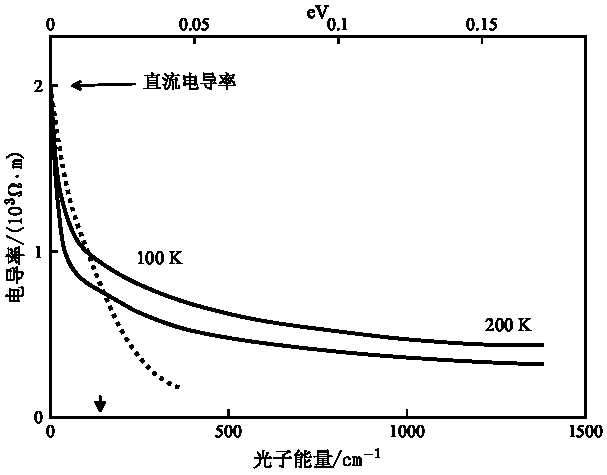
\includegraphics[width=8.5cm]{fig7-13.pdf}\\{\small 图 7.13\quad $\mathrm{YBa}_{2}\mathrm{Cu}_{3}\mathrm{O}_{7}$ 晶体的 $\sigma_{1}(\omega,T)$ 曲线，}\\[0.2em]
{\small 其中实线为实验曲线，点线是特鲁德公式的拟合，箭头表示的能量为 $k_{\mathrm{B}}\times200$ K}
\end{minipage}
\end{center}

显然，特鲁德公式也给出以 $\omega=0$ 为中心的尖峰，其峰的半宽度相当的光子 $\hbar\omega$ 应为 $\left(\hbar/\tau\right)$.为了再现远红外区的尖峰行为，可取 $\left(\hbar/\tau\right)\approx2k_{\mathrm{B}}T$ 作为一个初步的拟合.在图7.13中的点线是取 $T=100$ K 时特鲁德公式的拟合曲线，它与 $T=100$ K 的实验曲线在 $\hbar\omega<k_{\mathrm{B}}T$ 区内符合良好.在 $T=200$ K 的实验曲线左边的点线则是取 $T=200$ K 的特鲁德拟合曲线，它与实线在低频端的延伸也是一致的.这表明利用特鲁德公式作 $\left(\hbar/\tau\right)\approx2k_{\mathrm{B}}T$ 的简单拟合可以说明 $\sigma_{1}\left(\omega,T\right)$ 的尖峰行为.但是这个简单的拟合不能外推到 $\hbar\omega\gg k_{\mathrm{B}}T$ 的中红外区，在那里，$T=100$ K 的实验曲线与同一温度的特鲁德拟合曲线（点线）偏离较大，实验曲线的下降比特鲁德公式要缓慢得多.这表明 $\left(\hbar/\tau\right)\approx2k_{\mathrm{B}}T$ 拟合至少是不全面的，它没有反映出中红外区的平台特征.为了反映光电导谱的平台特征，人们采用了推广的特鲁德公式，即在式(7.7.7)基础上引入随频率 $\omega$ 变化的散射率 $1/\tau\left(\omega,T\right)$，用于拟合实验的 $\sigma\left(\omega,T\right)$ 曲线.一个与实验 $\sigma\left(\omega,T\right)$ 曲线良好符合的散射率公式是 $\hbar/\tau\left(\omega,T\right)=0.6\left(\pi k_{\mathrm{B}}T+\hbar\omega\right)$，等式右边第一项与简单拟合相近，既可以说明远红外区的尖峰特征，又可以再现 $\omega=0$ 时直流电阻率的测量值，新增加的第二项是散射率随 $\omega$ 的线性增长项，将阻止特鲁德导电率随 $\omega$ 增加而下降的趋势，形成中红外区 $\sigma_{1}$ 的平台特征.为了定性解释远红外与中红外区的光导电谱特征，通常采用一个比较宽松的唯象公式
\begin{equation}
  \left(\hbar/\tau\right)^{2}=\left(Ak_{\mathrm{B}}T\right)^{2}+\left(B\hbar\omega\right)^{2}
\end{equation}
式中A和B是数量级为1的常量.从上式不难看出，当 $\hbar\omega\ll k_{\mathrm{B}}T$ 时 $\left(\hbar/\tau\right)\sim k_{\mathrm{B}}T$，反之当 $\hbar\omega\gg k_{\mathrm{B}}T$ 时 $\left(\hbar/\tau\right)\sim\hbar\omega$，表明尖峰与平台特征均已纳入到这个唯象公式之中了.应当指出，在低温时从唯象公式导出的 $\left(1/\tau\right)\sim\omega$ 具有重要的物理内涵，其中 $\tau$ 是弛豫时间，在固体物理学中它是载流子的漂移速度按照 $v_{\mathrm{d}}(t)=v_{\mathrm{d}}(0)\mathrm{e}^{-t/\tau}$ 的指数规律衰减的特征时间，在相互作用的电子体系中（见第四章§11），这个 $\tau$ 也可称作准粒子（空穴或电子）的寿命，其倒数正比于准粒子自能的虚部.因此，可以从光电导实验的拟合求得高温超导体正常态的准粒子自能虚部正比于频率，即 $\mathrm{Im}\,\Sigma\sim\omega$，自能虚部的这一特征完全不同于普通金属所具有的朗道费密液体特征.对于朗道费密液体，在低温时根据式(4.11.15)，费密面附近的自能虚部 $\mathrm{Im}\,\Sigma_{\mathrm{FL}}\sim\omega^{2}$，其中取费密面为能量的原点.由此可知，铜氧化物在 $T_{\mathrm{c}}$ 之上的金属性正常态不能用朗道的费密液体理论描述.正是在这个意义上，人们常说高温超导体的正常态可能是一种非费密液体状态.

\subsection*{3. 核自旋-点阵弛豫率的反常}

核磁共振实验中的自旋-点阵弛豫率 $T_{1}^{-1}$ 是表征核自旋磁化强度 $\boldsymbol{M}(t)$ 从偏离平衡（由于外磁场的突然撤除与接入）的状态趋向于平衡值 $\boldsymbol{M}_{0}$ 的速率
\begin{equation}
  \frac{\mathrm{d}M(t)}{\mathrm{d}t}=\frac{\left[M_{0}-M(t)\right]}{T_{1}}
\end{equation}
或者用于描述 $M(t)$ 解的时间演化规律
\begin{equation}
  \left|M(t)-M_{0}\right|\sim\exp\left(\frac{-t}{T_{1}}\right)
\end{equation}
其中 $T_{1}$ 又称为自旋-点阵弛豫时间.这里人们用“自旋-点阵”术语是由于弛豫的机制来源于核自旋系统与点阵晶格系统之间的散射互作用.这是一种测量磁响应的有力工具，它可以提供晶体中不同核自旋的格点上电子态的信息.例如，在铜氧化合物高温超导体中，通过对导电层平面上 $^{63}\mathrm{Cu}$ 与 $^{17}\mathrm{O}$ 等格点上核弛豫率 $T_{1}^{-1}$ 的测量，可以提供其超导与正常态电子特征的重要信息.

在金属晶格中，核自旋与传导电子（属于点阵系统）之间的散射是产生自旋-点阵弛豫的主要机制.在朗道费密液体理论中，由于费密面的存在，必然导致正常金属的 $T_{1}^{-1}$ 正比于T，或 $T_{1}(T)\cdot T=$ 常数的柯林嘎（Korringa）关系.在推导此关系时，应当注意一个重要的差别，即核磁矩在磁场中的能级分裂 $\left(E_{m}-E_{n}\right)$ 远远小于电子自旋矩的相应能级分裂，这是由于质子质量比电子重1836倍，相应的核磁子 $\mu_{\mathrm{n}}$ 将比电子的玻尔磁子 $\mu_{\mathrm{B}}$ 要小相同的倍数.

现在简要介绍，在普通金属中柯林嘎关系的理论推导.核自旋与传导电子之间的相互作用由接触势描述，它与第十一章中将要介绍的局域自旋与传导电子间的 s-d（或 s-f）交换作用十分相似，可写成
\begin{equation}
  H_{\mathrm{int}}=V\cdot\boldsymbol{I}\cdot\hat{\boldsymbol{\sigma}}
\end{equation}
其中 $\boldsymbol{I}$ 是核自旋，$\hat{\boldsymbol{\sigma}}$ 为传导电子自旋泡利矩阵的矢量表示式，而V代表这个接触势的互作用强度.核自旋系统与传导电子的散射过程如图7.14所示.

当发生散射时，核自旋将偏转而在其磁场分裂能级 $E_{m}$ 与 $E_{n}$ 之间跳跃，这时电子的动量 k 与自旋s也将改变.当核自旋从量子态m跃迁到n的同时，传导电子将从初态 $\left|\boldsymbol{k},s\right\rangle$ 散射到终态 $\left|\boldsymbol{k}',s'\right\rangle$，所对应的电子能量分别为 $\varepsilon_{ks}$ 与 $\varepsilon_{k's'}$.核自旋-点阵的弛豫率可利用 $H_{\mathrm{int}}$ 的二级微扰理论写出
\begin{equation}
\begin{aligned}
  T_{1}^{-1}(T)&\sim\frac{2\pi}{\hbar}\sum_{k,k'}\sum_{s,s'}
  \left|\left\langle m,\boldsymbol{k},s\mid V\mid n,\boldsymbol{k}',s'\right\rangle\right|^{2}
  f\left(\varepsilon_{ks}\right)\times\\
  &\quad\left[1-f\left(\varepsilon_{k's'}\right)\right]\cdot
  \delta\left(E_{m}-E_{n}+\varepsilon_{ks}-\varepsilon_{k's'}\right)
\end{aligned}
\end{equation}

\begin{center}
\begin{minipage}{6cm}
\centering
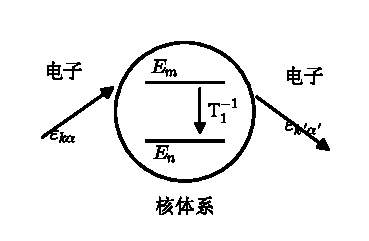
\includegraphics[width=6cm]{fig7-14.pdf}\\{\small 图 7.14\quad 核自旋系统与传导电子的散射过程}
\end{minipage}
\end{center}

其中包括了来自泡利不相容原理的概率因子 $f(\varepsilon)\left[1-f(\varepsilon')\right]$ 和保证散射过程总能量守恒的 $\delta$ 函数因子.由于在磁场中核自旋的能级差 $\left(E_{m}-E_{n}\right)$ 是一个可忽略的小量，它比 $k_{\mathrm{B}}T$ 和化学势 $\mu$ 均要小得多，可以认为散射前后电子态能量近似守恒，即可取近似 $\varepsilon_{k's'}\approx\varepsilon_{ks}\equiv\varepsilon$，这时式(7.7.12)中 $\delta$ 函数简化为 $\delta\left(\varepsilon_{ks}-\varepsilon_{k's'}\right)$.再进而考虑到，在实验温度范围内，总有 $k_{\mathrm{B}}T\ll\mu$，又可将概率因子演化为 $f(\varepsilon)\left[1-f(\varepsilon)\right]=\left(k_{\mathrm{B}}T\right)\left[-\mathrm{d}f(\varepsilon)/\mathrm{d}\varepsilon\right]\approx\left(k_{\mathrm{B}}T\right)\delta\left(\varepsilon-\mu\right)$.运用这两个 $\delta$ 函数，经求和化积分后，即可从式(7.7.12)求得 $T_{1}^{-1}(T)\propto T$ 的简单结果，此即柯林嘎关系 $T_{1}(T)\cdot T=$ 常数.

为使读者明白柯林嘎关系的成立是朗道费密液体行为的表现，可直接从金属的费密球模型（即费密液体模型）出发，对 $T_{1}^{-1}(T)$ 的特征作如下的定性解释：根据泡利原理，只有位于费密面附近 $\left(k_{\mathrm{B}}T\right)$ 范围内的传导电子才可以参与散射，即只占全部传导电子数的一个分数 $\left(k_{\mathrm{B}}T/\mu\right)$.引入费密面上态密度 $N(\mu)$，求得与核自旋发生散射的传导电子数为 $N(\mu)\left(k_{\mathrm{B}}T/\mu\right)$，它与接触势强度的模平方 $\left|V\right|^{2}$ 都应当是正比于核弛豫率的关键参数，由此立刻得到柯林嘎关系式：
\begin{equation}
  T_{1}^{-1}(T)\sim\left|V\right|^{2}\cdot N(\mu)\cdot\left(k_{\mathrm{B}}T/\mu\right)\propto T
  \qquad\text{或}\quad T_{1}(T)\cdot T=\text{常数}
\end{equation}
因此，柯林嘎关系的出现是与金属中存在费密面直接相关联的.在常规BCS超导体中，核自旋-点阵弛豫率的柯林嘎关系在 $T>T_{\mathrm{c}}$ 时普遍成立，表明其正常态具有费密液体行为.

在以 $\mathrm{YBa}_{2}\mathrm{Cu}_{3}\mathrm{O}_{7}$ 为代表的铜氧化合物高温超导体中，人们却观察到其正常态核自旋-点阵弛豫率的异常行为，特别是对于导电层中 $^{63}\mathrm{Cu}$ 的 $T_{1}^{-1}$ 测量，来自各著名研究组的数据基本上是一致的，均表明Y-123最佳化合物在 $T>T_{\mathrm{c}}$ 温区的核弛豫率满足经验公式
\begin{equation}
  T_{1}^{-1}(T)=aT+b
\end{equation}
其中a和b都是与温度无关的常数.在上式右边，随温度线性变化的 $aT$ 项与普通金属的柯林嘎行为定性一致，奇异之处在于出现了不随温度变化的常数b项，导致 $^{63}\mathrm{Cu}$ 的核弛豫明显偏离柯林嘎关系，呈现出不同于朗道费密液体的反常特征.使问题变得复杂的是，测量位于同一导电层中 $^{17}\mathrm{O}$ 的核弛豫，却表明其 $T_{1}^{-1}$ 是满足柯林嘎关系的，对于 $^{17}\mathrm{O}$ 没有异常项b出现.在Y-123最佳化合物中，位于同一个 $\mathrm{CuO}_{2}$ 平面上的 $\left(1/T_{1}\right)_{\mathrm{Cu}}$ 具有明显的非柯林嘎行为，而 $\left(1/T_{1}\right)_{\mathrm{O}}$ 则表现柯林嘎行为，二者有如此显著的定性差别，其理论解释自然应超出朗道费密液体范围.一个新的理论必须同时解释 $\left(1/T_{1}\right)_{\mathrm{Cu}}$ 的非费密液体特征和 $\left(1/T_{1}\right)_{\mathrm{O}}$ 的正常费密液体行为.

\subsection*{4. 反铁磁费密液体模型}

目前，在解释高温超导体核弛豫实验方面，比较成功的理论模型是密立斯（Millis）、莫尼恩（Monien）和派因斯（Pines）\textsuperscript{[33]}（MMP）提出的反铁磁费密液体（AFL）理论.他们假定在 $\mathrm{CuO}_{2}$ 平面内每个元胞只含一个 $S=1/2$ 的电子自旋自由度，其中心在Cu格点上，并且诸Cu格点的电子自旋之间存在着短程的反铁磁关联和相应的自旋涨落效应，这一关联使近邻Cu格点的电子自旋取向基本相反.密立斯等人认为正是Cu格点上的电子自旋与各类核磁矩的相互作用产生铜氧化合物中的核自旋-点阵弛豫.对于Cu的核弛豫，主要是考虑 Cu 核与同格点电子自旋的相互作用，可求出 $\left(1/T_{1}\right)_{\mathrm{Cu}}$ 的非柯林嘎关系，与经验公式(7.7.14)一致，其中不随温度变化的常数项b是反铁磁关联的自旋涨落效应产生的，从而解释了 $\left(1/T_{1}\right)_{\mathrm{Cu}}$ 的异常温度行为.对于O的核弛豫，则需要考虑O核与两个近邻Cu格点上的电子自旋互作用，因为在 $\mathrm{CuO}_{2}$ 平面中O位于两个近邻Cu格点之间，Cu与O的键长只是晶格常数的一半 $\left(a/2\approx0.2\ \mathrm{nm}\right)$，应有较强的互作用.但由于存在反铁磁关联，O的两近邻Cu格点的电子自旋取向相反，它们与O核磁矩的互作用将大部分相互抵消，导致在 $\left(1/T_{1}\right)_{\mathrm{O}}$ 中与温度无关的异常项消失，只剩下与温度成正比的柯林嘎项.这样MMP理论就同时解释了高温超导体中 Cu 与 O 的核弛豫的不同温度行为.

密立斯等人的反铁磁费密液体理论，只是在朗道费密液体理论基础上计入了反铁磁自旋涨落关联的修正.反铁磁费密液体理论，从本质上讲，仍属于费密液体范畴，我们仍可以沿袭前面的定性说法来理解核弛豫率异常的成因.当不计反铁磁关联时，反铁磁费密液体系统自然简化为朗道费密液体，这时费密面上的态密度基本上是与温度无关的常数，而参加散射的电子自旋激发仍然应限制在费密面附近 $k_{\mathrm{B}}T$ 范围内，于是得到弛豫率 $T_{1}^{-1}(T)\sim T$ 的柯林嘎关系，与式(7.7.13)相同.但是，当计入反铁磁自旋关联效应之后，由于关联随温度降低而增强，将对态密度产生重要的影响，使其中出现一个附加项 $\Delta N\left(\mu,T\right)\sim1/T$，表明低频自旋激发的态密度也将随温度降低而升高，正是此项与限制自旋激发范围的T因子相消，给出 Cu 核弛豫率的常数项b，导致 $\left(1/T_{1}\right)_{\mathrm{Cu}}$ 的非柯林嘎行为.在讨论O的核弛豫率时，由于来自两近邻Cu格点的反铁磁关联效应在O位上相互抵消，态密度仍与温度无关，这时 $\left(1/T_{1}\right)_{\mathrm{O}}$ 仍然满足柯林嘎关系，无异常行为.

密立斯等人的反铁磁费密液体理论不仅能正确解释Y-123与 La-214 等铜氧化合物中核自旋-点阵弛豫率的反常特性，还同时解释了核磁共振中的奈特（Knight）位移等磁响应实验.将该理论推广用于导电等电荷响应问题也获得了成功，例如在直流电阻率的讨论中，按照MMP模型应考虑载流子与位于Cu格点上的电子自旋自由度的耦合，文献\textsuperscript{[23]}中具体计算了载流子与反铁磁自旋涨落元激发（这种元激发在文献中称为反铁磁 paramagnons）散射的电阻率，所求得的零频 $\left(\omega=0\right)$ 散射率在 $T_{\mathrm{c}}$ 之上总能够满足 $\left(\hbar/\tau\right)\sim T$ 规律，合理说明了正常态的直流电阻率在相当宽阔的温区内是温度的线性函数.在这里是反铁磁自旋涨落（AFSF）机制产生电阻率反常，究其本源是电子系统内部的库仑关联作用所产生的.值得一提的是，载流子间通过交换反铁磁自旋涨落也可以产生有效吸引互作用，并且有利于形成 $d_{x^{2}-y^{2}}$ 波超导配对\textsuperscript{[23]}.到此为止，建立在反铁磁费密液体理论基础上的自旋涨落机制既能够说明正常态的电阻反常，又可以解释d波配对的形成，应当说对于最佳掺杂的高温超导体是一个有竞争力的理论.但是，最近在弱掺杂区发现的正常态能隙却对此理论提出了新的挑战，为此派因斯等人\textsuperscript{[34]}又提出了新的唯象假定，尚待实验证实.

\section{弱掺杂区正常态赝隙的发现}

根据§7中关于最佳掺杂样品的讨论，已使人们认识到高温超导体正常态的性质是十分反常的，需要用一个不同于朗道费密液体的理论描述.然而，当人们将注意力集中到相图中的弱掺杂区域时（见图7.5，其中最佳掺杂对应于最高的 $T_{\mathrm{c}}$ 点，其左边就是弱掺杂区，而右边称为过掺杂区），却观察到一个更令人吃惊的反常现象——在弱掺杂区的正常态（$T>T_{\mathrm{c}}$）中已经形成了能隙.换句话说，在通常情况下显示系统在 $T=T_{\mathrm{c}}$ 时进入超导态的能隙，现已在远远高于实际形成超导电性的温区内被观察到了.正常态能隙在文献中又称赝隙（pseudogap），所谓赝隙是指部分形成能隙，例如在单电子近似成立的能带论中，部分能隙说的是在费密面的部分区域中形成了能隙，而在其它区域中未成隙，系统仍保持金属性电导特征.尽管早期的观察仅在弱掺杂的YBCO（即弱掺杂的Y-123）样品中看到正常态有赝隙存在的迹象，但自从1996年当人们用ARPES直接测出赝隙存在之后，来自各不同实验组的测量结果均证实了一个共同的现象\textsuperscript{[31]}，即在所有弱掺杂的铜氧化合物高温超导体的正常态中均存在赝隙，这是弱掺杂区正常态的一个基本属性.

\subsection*{1. 弱掺杂区存在赝隙的间接证据}

1989年在测量弱掺杂 Y-123 导电层中铜（$^{63}\mathrm{Cu}$）的自旋-点阵弛豫率时，人们首次观察到赝隙存在的迹象.图7.15同时给出了 $T_{\mathrm{c}}=90$ K 的最佳掺杂样品 $\mathrm{YBa}_{2}\mathrm{Cu}_{3}\mathrm{O}_{7}$（□）和 $T_{\mathrm{c}}=60$ K 的弱掺杂样品 $\mathrm{YBa}_{2}\mathrm{Cu}_{3}\mathrm{O}_{6.7}$（○）中 $^{63}\mathrm{Cu}$ 的 $\left(T_{1}T\right)^{-1}$ 随温度的变化曲线.显然，在 $T_{\mathrm{c}}$ 以上最佳化合物正常态的 $\left(T_{1}T\right)^{-1}$ 随温度降低而增大并一直延伸到 $T_{\mathrm{c}}=90$ K 处，这是反铁磁自旋关联在降温时增强所产生的正常态非柯林嘎行为，可以用式(7.7.14)描述.当温度下降到 $T_{\mathrm{c}}$ 时，$\left(T_{1}T\right)^{-1}$ 曲线的明显转折和进入超导态后（$T<T_{\mathrm{c}}=90$ K 时）曲线的急剧下降则表明：在发生正常-超导相变的同时，载流子因配对形成了能隙，导致态密度的亏损，从而压制了Cu格点上电子自旋的激发，使 $\left(T_{1}T\right)^{-1}$ 曲线急剧下降.对于 $T_{\mathrm{c}}=60$ K 弱掺杂样品，在 $T>150$ K 的高温端的非柯林嘎行为与最佳化合物正常态的反常行为极其相似，这一反常仍来源于温度下降时AF自旋关联的增强效应，但是在 $150\ \mathrm{K}>T>100\ \mathrm{K}$ 的中间温区 $\left(T_{1}T\right)^{-1}$ 随温度缓慢变化并有一个极大值宽峰，表现出与 $T_{\mathrm{c}}=90$ K 最佳化合物明显的不同.然后当 $T<100$ K 时，尽管弱掺杂样品仍处于正常态，其 $\left(T_{1}T\right)^{-1}$ 已开始下降，而且是连续地下降和经过 $T_{\mathrm{c}}$（$T_{\mathrm{c}}=60$ K）进入超导态.在弱掺杂的 $T_{\mathrm{c}}=60$ K 样品中，$\left(T_{1}T\right)^{-1}$ 从正常态的某一温度 $T^{*}$（$T^{*}>T_{\mathrm{c}}$）所开始的连续下降与最佳化合物进入超导态后的下降趋势也是定性一致的.弱掺杂样品的这种不同寻常的中间温区自旋-点阵弛豫行为被认为是载流子在正常态的某一温度 $T^{*}$ 处已开始预配对并形成了能隙，这是显示正常态存在赝隙的第一个间接证据.

\begin{center}
\begin{minipage}{7cm}
\centering
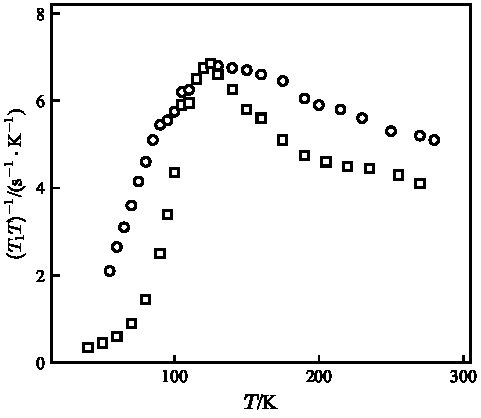
\includegraphics[width=7cm]{fig7-15.pdf}\\{\small 图 7.15\quad $\mathrm{YBa}_{2}\mathrm{Cu}_{3}\mathrm{O}_{6+x}$ 中 $^{63}\mathrm{Cu}$ 的核自旋-点阵弛豫率，其中最佳掺杂（□）为 $x=1$，}\\[0.2em]
{\small 弱掺杂（○）为 $x=0.7$}
\end{minipage}
\end{center}

另一个显示弱掺杂区存在赝隙的间接证据来自对导电层中直流电阻率 $\rho_{\mathrm{ab}}$ 的测量，图7.16是 $\mathrm{La}_{2-x}\mathrm{Sr}_{x}\mathrm{CuO}_{4}$ 在各种掺杂浓度x时的 $\rho_{\mathrm{ab}}$-$T$ 曲线，其中除最佳掺杂 $\left(x=0.15\right)$ 情形外，还包括了弱掺杂 $\left(x<0.15\right)$ 和过掺杂 $\left(x>0.15\right)$ 情形.在图7.16(a)中可以看出，除了 $x=0.15$ 曲线在 $T_{\mathrm{c}}$ 之上具有线性温度行为以外，其它的弱掺杂样品均在某一温度 $T^{*}(x)$ 之下明显偏离线性，并且 $T^{*}(x)$ 随x减小而升高，其中 $x<0.07$ 的那些曲线已不是超导样品，它们的基态为绝缘体.图7.16(b)主要显示过掺杂 La-214 系统 $\left(x>0.15\right)$ 的电阻率温度行为，这时随着x的逐渐增大 $T_{\mathrm{c}}$ 连续降低，最后在 $x=0.3$ 时变为非超导的正常金属，而其低温电阻率则演变为具有 $\rho_{\mathrm{ab}}\sim T^{2}$ 特征的朗道费密液体，与本章§2中所介绍的相图特征一致.

\begin{center}
\begin{minipage}{9cm}
\centering
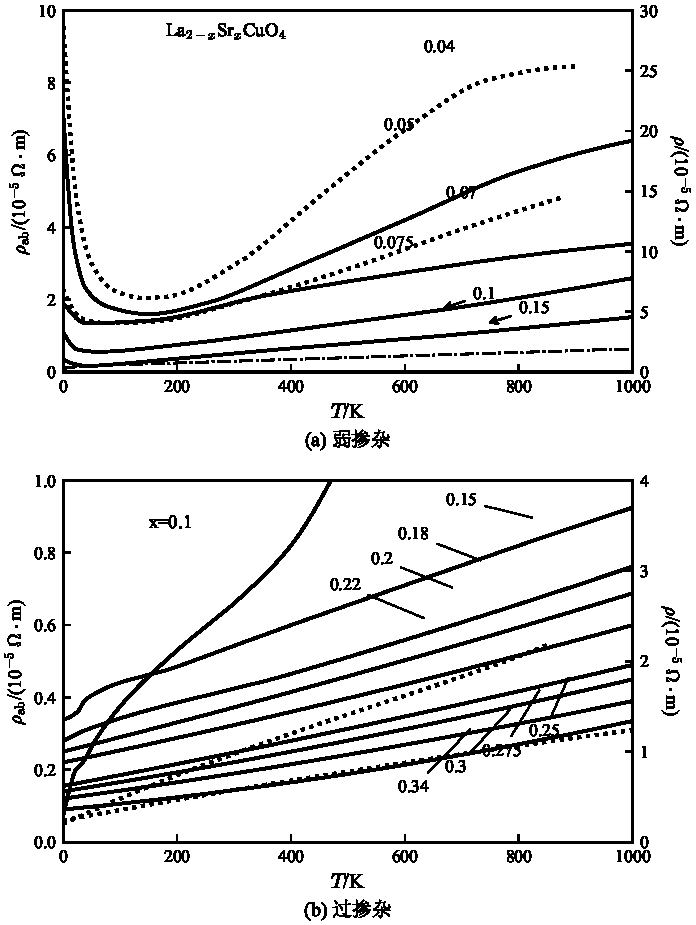
\includegraphics[width=9cm]{fig7-16.pdf}\\[0.3em]
{\small (a) 弱掺杂\qquad\qquad\qquad\qquad (b) 过掺杂}\\[0.2em]
{\small 图 7.16\quad $\mathrm{La}_{2-x}\mathrm{Sr}_{x}\mathrm{CuO}_{4}$ 在各种掺杂浓度 x 时的 $\rho_{\mathrm{ab}}$-$T$ 曲线}\\[0.2em]
{\small 其中点线为单晶（左标），实线代表多晶样品（右标）}
\end{minipage}
\end{center}

弱掺杂的 La-214 中电阻率偏离线性温度规律的特征在弱杂的Y-123化合物中也同样存在，考虑到正常态的线性电阻率可以用载流子被自旋涨落散射机制解释，在弱掺杂时电阻率在 $T<T^{*}$ 温区偏离线性温度律的更快降落也可以认为是由于在正常态形成了能隙，使自旋涨落效应受到压制的缘故，但是根据核弛豫率和电阻率实验来断言赝隙的存在都是间接的，带有一定的人为猜测性，还需要有赝隙存在的直接证据.

\subsection*{2. 弱掺杂区存在赝隙的直接证据}

角分辨光电子发射谱（简称ARPES）是直接测量准粒子态密度随能量和动量变化的有力工具.对于超导体运用APRES技术可以直接确定能隙的大小及其随取向 $\hat{\boldsymbol{k}}$ 的变化.因为当系统进入超导态后，能隙出现在准粒子的态密度中，这时 k 态的态密度将在低于费密能的某个能量［即能隙 $\Delta(\boldsymbol{k})$］范围内下降为零，相当于使态k态的态密度向低能方向移动而离开费密能，实验上表现为ARPES谱线前沿（leading edge）的中点有相应的移动.在§3中，人们正是测量ARPES谱的这一移动，定出了二维BZ中能隙 $\Delta(\boldsymbol{k})$ 随取向的变化，首次观察到铜氧化合物高温超导体的各向异性配对特征.因此，ARPES是直接测量能隙的一个重要手段.如果在欠掺杂铜氧化合物的正常态中确实存在能隙，其最为直接的证据应来自ARPES测量.1996年美国斯坦福大学研究组\textsuperscript{[35]}和阿贡研究组\textsuperscript{[36]}利用ARPES在 Bi-2212 欠掺杂样品中，都清楚地观测到在正常态中打开能隙的直接证据，并且这个正常态赝隙也具有 $d_{x^{2}-y^{2}}$ 波对称性（即沿 $k_{x}$ 与 $k_{y}$ 方向能隙取最大值，沿对角线 $\left|k_{x}\right|=\left|k_{y}\right|$ 方向则为能隙的零点），与§3中所介绍的最佳化合物在 $T_{\mathrm{c}}$ 以下的超导能隙具有相同的各向异性 $\left(d_{x^{2}-y^{2}}\right.$ 波）特征.他们的测量还表明：正常态能隙的起始温度随掺杂增加而减小，当系统成为最佳化合物时 $T^{*}$ 已十分接近 $T_{\mathrm{c}}$，这时在ARPES实验中已观察不到最佳掺杂以及过掺杂区的正常态能隙，可以认为在正常态出现赝隙只是弱掺杂区的特征.图7.17是考虑了弱掺杂区存在正常态赝隙的示意相图，正常态赝隙只出现在弱掺杂区，当系统进入最佳与过掺杂区时赝隙实际上已消失，只剩下 $T<T_{\mathrm{c}}$ 时的超导能隙.这时系统形成能隙与进入超导态几乎是同时发生的，而且在 $T=T_{\mathrm{c}}$ 时超导能隙消失，与常规BCS超导体的正常-超导转变特征相似.此外，在过掺杂区内BCS的普适关系 $\left[2\Delta(0)/k_{\mathrm{B}}T_{\mathrm{c}}\right]=$ 常数仍然成立.

\begin{center}
\begin{minipage}{7.5cm}
\centering
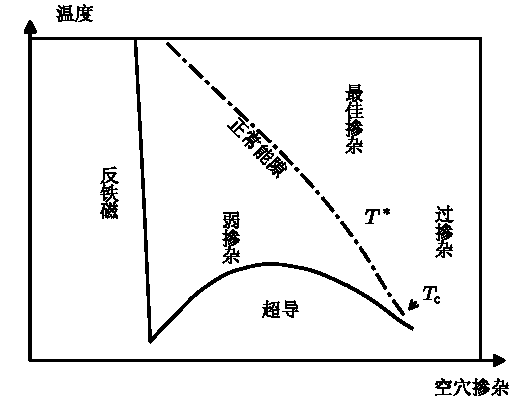
\includegraphics[width=7.5cm]{fig7-17.pdf}\\{\small 图 7.17\quad 计入赝隙的示意相图}
\end{minipage}
\end{center}

在弱掺杂样品中的ARPES测量直接证实了正常态能隙的存在当然是一个重要的新发现，但却是不出人们所料的结果.令人感到十分惊奇的是，还发现了下列完全不同于BCS超导相变的特征：其一是正常态赝隙（PG）仅在超过起始温度 $T^{*}$ 时（对于弱掺杂的 Bi-2212，$T^{*}$ 在170～300 K之间）才迅速下降为零，在 $T<T^{*}$ 的大部分正常区域中PG几乎不随温度变化，而且正常态PG的数值与 $T\ll T_{\mathrm{c}}$ 时的超导能隙值相近.包括ARPES在内的多种实验均已证实\textsuperscript{[31]}，随着温度降低正常态的PG平坦连续地演变为超导能隙，特别当温度经过 $T_{\mathrm{c}}$ 时能隙的数值并无显著的变化.换句话说，没有任何实验证据表明弱掺杂区中超导能隙在 $T=T_{\mathrm{c}}$ 处降为零，从根本上不同于BCS超导体的序参数特征.在BCS超导体中，表征序参数的超导能隙在 $T_{\mathrm{c}}$ 处应消失，即有 $\Delta_{\mathrm{BCS}}\left(T_{\mathrm{c}}\right)=0$ 关系.其二是ARPES的测量还表明：在弱掺杂区域中在掺杂增加（即 $T_{\mathrm{c}}$ 升高）的同时，正常态的PG与零温的超导能隙均不按比例增大，反而呈现微弱的下降趋势，这种异常的变化趋势完全与BCS理论的预言相反，在BCS超导体中，零温超导能隙值应与 $T_{\mathrm{c}}$ 值成正比，并存在 $\left[2\Delta_{\mathrm{BCS}}(0)/k_{\mathrm{B}}T_{\mathrm{c}}\right]=$ 常数的普适关系，但是对于弱掺杂的铜氧化合物高温超导体，这一BCS的普适关系已不成立.正如安德逊所指出：“在这里的情形已不再是BCS理论所能解释的，尽管仍然存在库柏对，但其相变的物理内涵已与常规超导体的行为相去甚远，已经不能再称为BCS超导相变了.”\textsuperscript{[37]}

\subsection*{3. 小结与讨论}

尽管以上所介绍的赝隙测量主要是在含有两个 $\mathrm{CuO}_{2}$ 层的 Y-123 及 Bi-2212 欠掺杂化合物中作出的，但随后的实验表明，无论是在含单 $\mathrm{CuO}_{2}$ 层的 Hg-1201 及 La-214 中，或者是在含有三个 $\mathrm{CuO}_{2}$ 层的 Hg-1223 等弱掺杂化合物中都观察到与双层弱掺杂化合物中相似的赝隙特征.我们可以说，存在正常态赝隙是所有铜氧化合物高温超导体在弱掺杂区的普遍特征.无论是关于自旋响应，还是关于电荷响应的测量均已证实存在一个特征温度 $T^{*}$，它远比 $T_{\mathrm{c}}$ 高得多，在这个温度处出现正常态的配对，形成赝隙.赝隙存在于正常态的 $T^{*}<T<T_{\mathrm{c}}$ 温区之内.在弱掺杂区，当掺杂浓度增加时，$T_{\mathrm{c}}$ 升高，赝隙的起始温度 $T^{*}$ 则随之下降，在最佳掺杂时两者已十分接近，一旦进入过掺杂区，$T^{*}$ 即并入 $T_{\mathrm{c}}$ 曲线，这时已观察不到正常态的赝隙.因此，图7.17中的 $T^{*}$ 与 $T_{\mathrm{c}}$ 曲线构成了赝隙区的边界，它主要出现在弱掺杂区.实验还证实正常态赝隙与超导能隙具有相同的d波对称性，而且没有任何证据说明超导能隙在转变温度 $T_{\mathrm{c}}$ 处可能降为零.因此在铜氧化合物高温超导体的弱掺杂区域中，在正常态的 $T^{*}$ 温度以下已经形成了配对，并显示出赝隙的存在，但还没有发展成为一个长程相干的库柏对系统，只有在更低的温度 $T_{\mathrm{c}}$ 之下才能形成库柏对间的相位相干，并发生超导凝聚.在这里对的形成与超导凝聚不是同时发生的，它们将分成两步在不同的温度上发生.这是与BCS完全不同的图像，在BCS理论中，对的形成与相位相干是同时发生的.但是，在欠掺杂的铜氧化合物中，实验已证明当尚未发生超导凝聚时，在正常态已有能隙打开，这表明在正常态首先形成了电子间的“预配对”，而后才发生相干凝聚进入超导态.更确切地说，在正常态的“预配对”观点是人们根据弱掺杂区普遍存在赝隙现象所达成的共识.

最早提出的“预配对”模型是安德逊的共振价键（resonating valence bond 以下简称RVB）模型\textsuperscript{[38]}.首先说明，所谓价键态是指两个自旋间配对所形成的单重态，在价键（VB）态基础上将所有可能的自旋单重态配对波函数按照量子力学的叠加原理作线性组合就构成共振价键态.安德逊认为在掺杂的铜氧化合物中RVB态比反铁磁奈耳（Neel）态更稳定和更接近系统的基态，因此他建议从RVB态出发讨论高温超导电性.在未掺杂的RVB态中，每个格点上有一个电子，这个电子的自旋自由度与另一格点上电子的自旋配对，组成总自旋为零的自旋单态，而RVB的基态波函数就是点阵中的不同格点间的自旋单重配对态的线性组合，这时系统中的每一个自旋都被冻结在单重配对态之中，从而构成RVB理论中电中性的“真空”.现在若从此“真空”中某格点上取出一个电子（即进行空穴掺杂），则相对于RVB“真空”讲，在此格点上将出现一个无自旋但带有 $\left(+e\right)$ 电荷的准粒子（即空穴子），与此同时还有另一个格点上的自旋由于失配而不能形成自旋单态，相对于RVB“真空”在失配的格点上将出现一个带有 $S=1/2$ 自旋但无电荷的准粒子（即自旋子）.安德逊认为空穴子（holons）与自旋子（spinons）是RVB背景上的两种相对独立运动的准粒子，它们分别反映电荷自由度与自旋自由度的运动特征，此即文献中经常提到的电荷与自旋分离假说.在这个意义上人们常说RVB图像是一个基于自旋与电荷分离假定的模型.由于在RVB图像中自旋自由度的单重态配对已经在远高于 $T_{\mathrm{c}}$ 时形成，必然导致在自旋激发谱中出现正常态的能隙，对应于实验上观察到的赝隙或自旋能隙（spin gap），而超导电性的出现还取决于空穴子之间的相干性，仅当空穴子在 $T_{\mathrm{c}}$ 时成为相位相干时，系统才能凝聚为超导态.在强关联电子系统中，常采用费密子描述有自旋但无电荷的自旋子，而将带有电荷却无自旋的空穴子当作带电玻色子，因此人们认为在RVB态上的超导就是荷电玻色子的玻色凝聚.但应明白，这是在已经形成自旋单重态配对基础上的空穴子凝聚.在第十一章中我们将介绍基于RVB态的一个高温超导平均场理论（§10），用于定量解释在弱掺杂区形成赝隙（即预配对）与超导凝聚（即玻色凝聚）发生在不同的温度.目前RVB理论已超出平均场近似，其中受到人们普遍关注的是李雅达等人提出的规范场理论\textsuperscript{[39]}.RVB理论中最基本的假定是认为在二维强关联电子体系中存在电荷与自旋分离的两种元激发.但是这个基本假定还有待于实验的证实，而理论上则涉及二维拉亭格液体的研究\textsuperscript{[40]}.人们寄希望于二维拉亭格理论能够支持 $\mathrm{CuO}_{2}$ 平面上的自旋与电荷分离假定.

\begin{canKao}
\begin{enumerate}[label={[\arabic*]}, leftmargin=2.2em, itemsep=0pt]
\item 章立源等. 超导物理. 北京: 电子工业出版社，1987
\item Bednorz J D, Müller K A. Z Phys, 1986, B64: 189
\item Wu M K, Chu C W et al. Phys Rev Lett, 1987, 58: 908
\item 赵忠贤等. 科学通报，1987，32：412
\item Chu C W et al. Phys Rev Lett, 1988, 60: 941
\item Sheng Z Z et al. Phys Rev Lett, 1988, 60: 937
\item Tokura Y et al. Nature, 1989, 337: 345
\item Ginsberg D M. Physical Properties of High Temperature Superconductors (Vol IV). Singapore: World Scientific, 1994. 3
\item Levi B G. Phys Today, 1994, 47: 17
\item Gunnarsson O. Nature, 2000, 408: 528
\item Schön J H, Kloc Ch, Batlogg B. Nature, 2000, 408: 549; Science, 2001, 23: 2432
\item Bud'ko S L et al. Phys Rev Lett, 2001, 86: 1877
\item 韩汝珊. 高温超导物理. 北京: 北京大学出版社，1998
\item Zhang S C. Science, 1997, 275: 1089
\item Batlogg B. Phys Today, 1991, 44: 44
\item Shen Z X et al. Phys Rev Lett, 1993, 70: 1553
\item Wollman D A, van Harlingen D J et al. Phys Rev Lett, 1993, 71: 2134; 1995, 74: 797
\item Mathai A, Wellstood F C et al. Phys Rev Lett, 1995, 74: 4523
\item Tsuei C C, Kirtley F C et al. Phys Rev Lett, 1995, 73: 593
\item Kouznetsov K A et al. Phys Rev Lett, 1997, 79: 3050
\item Meservey R, Schwartz B B. Superconductivity (Vol 1). New York: Marcel Dekker Inc, 1969. 126
\item Frank J P et al. Ginsberg D M, ed. Physical Properties of High Temperature Superconductivity (Vol IV). Singapore: World Scientific, 1994. 189
\item Scalapino D J. Physics Reports, 1995, 250: 329
\item Tsuei C C et al. Phys Rev Lett, 1990, 65: 2724
\item Anderson P W, Morel P. Phys Rev, 1961, 123: 1911
\item Varma C M. Comments Solid State Phys, 1985, 11: 221
\item Stewart G R. Rev Mod Phys, 1984, 56: 755
\item Grewe N, Steglich F. Handbook on the Physics and Chemistry of Rare Earths, 1991, 14: 343
\item 邢定钰. 张其瑞主编. 高温超导电性. 杭州: 浙江大学出版社，1992. 第四章
\item Ziman J M. Electrons and Phonons. London: Oxford Univ Press, 1960. 364
\item Timusk T et al. Rep Prog Phys, 1999, 62: 61
\item Burns G. Solid State Physics. Orlando: Academic Press, 1985
\item Millis A J, Monien H, Pines D. Phys Rev, 1990, B44: 167
\item Pines D. Z Phys, 1997, B103: 129
\item Loeser A G et al. Science, 1996, 273: 325
\item Ding H et al. Nature, 1996, 382: 51
\item Levi B G. Phys Today, 1996, 49: 17
\item Anderson P W. Science, 1987, 235: 1196
\item Lee P A et al. Phys Rev Lett, 1997, 78: 4111
\item Anderson P W. Phys Rev Lett, 1991, 67: 2092
\end{enumerate}
\end{canKao}

% ============================================================
%  第八章 能带论（§1–§11 + 章末参考文献）
%  底本：高等教育出版社《固体理论》第二版；原书印刷页 287–342
%  （PDF 页 = 印刷页 + 20）
%  公式编号自检：§1 (8.1.1)–(8.1.13)；§2 (8.2.1)–(8.2.17)；
%    §3 (8.3.1)–(8.3.21)；§4 (8.4.1)–(8.4.10)；§5 (8.5.1)–(8.5.44)；
%    §6 (8.6.1)–(8.6.25)；§7 (8.7.1)–(8.7.16)；§8 (8.8.1)–(8.8.30)；
%    §9 (8.9.1)–(8.9.25)；§10 (8.10.1)–(8.10.25)；
%    §11 (8.11.1)–(8.11.54)（其中 (8.11.8a/b)、(8.11.9a/b)、
%    (8.11.11a/b/c)、(8.11.20a–d)、(8.11.21a/b)、(8.11.22a/b)、
%    (8.11.25a/b/c)、(8.11.27a/b) 为原书自带二级编号，用
%    subequations 环境照录，与 ch04/ch06 体例一致）。
%    全章自动编号共 280 个编号公式。
%
%  任务单所列 13 处"缺号"逐条对照原书页面判定（均非原书跳号，
%  公式全部在原书中，只是 OCR 的 tag 残缺或粘连，已按页面归位）：
%    (8.2.7)  原书 p291 在号（OCR tag 残为 {2.7}）；
%    (8.2.12) 原书 p292 在号（OCR tag 残为"( 8 ."）；
%    (8.2.13) 原书 p292 在号，OCR 的 tag {8.2.13} 本就完整，不缺；
%    (8.3.13) 原书 p296 在号（p296 顶五行连等式），OCR 漏 tag 且
%             公式严重乱码，已按 p296 重排；
%    (8.6.6)  原书 p309 在号（编号 OCR 掉为正文行"（8.6.6）"）；
%    (8.6.7)  原书 p309 在号（OCR tag 残为 {6.7}）；
%    (8.6.15) 原书 p310 在号（OCR tag 残为 {6.15}）；
%    (8.6.24) 原书 p312 在号，OCR 的 tag 本就完整，不缺；
%    (8.8.13) 原书 p318 在号（OCR tag 残为 {8.13}）；
%    (8.9.5)  原书 p321 在号（编号 OCR 粘进公式末行）；
%    (8.10.8) 原书 p326 在号（OCR tag 残为 {10.8}）。
%
%  已修正的 OCR/原书错误（除全角句点转"."、删 ~ 间隔符、收紧
%  \mathrm{d}、拆开行内公式与中文等常规项外）：
%  1. §1 (8.1.3) 求和下标按原书为倒格矢 K（OCR 误作 k）；
%     (8.1.7)"(N2)^{-1/2}"→(NΩ)^{-1/2}；(8.1.11) 系数 a(k+K')
%     系原书排印如此（投影后指标未换），照录（p288）。
%  2. 表 8.1 表头"k_r = 0.589"→k_F = 0.589、"a(X)"→a(K)，各列
%     数据按 p288–289 复核；正文中"不同 1KI 值"→|K| 值、"A1"→Al。
%  3. §2 (8.2.9)"O_{1-}Σ<ψ_c|ψ_{c'}>"→(1-Σ_{c'}<ψ_c|ψ_{c'}>)（p291）；
%     (8.2.16)(8.2.17) 及其间三个未编号矩阵元式按 p293 重排，
%     (8.2.17) 末尾 OCR 脱落的因子 ×(ℏ²k²/2m + |E_{1s}|) 按 p293 补回。
%  4. §3.1"综上所述"→"综合上述"（p295）；p295 脚注①"因为离子实中
%     壳层电子波函数是振荡的……否则两者不能正交."OCR 漏失，按页脚补录。
%  5. §3.2 (8.3.9)–(8.3.12) 及 (8.3.13) 五行连等式按 p295–296 重排；
%     (8.3.14) 左矢按 p296 为 <ψ_k|（OCR 误作 φ_k）。
%  6. §3.3"光谱项一 a_M 致"→"光谱项一致"（OCR 衍字倒装，p298）；
%     (8.6.1) 第二分段条件"r≠r_i"→"r⩾r_i"（p309，丸盒势球外为零）。
%  7. §4 (8.4.2)(8.4.4)(8.4.7) 的 χ/χ_k 乱码按 p299–300 重排；
%     (8.4.7) OCR 拆成的两块按原书合并为一式（p299–300 跨页一式）；
%     正文"平滑的 x"→"平滑的 χ_k"（p299）。
%  8. §5 (8.5.9) r_。→r_s；(8.5.16)"d/r dτ"→(1/r)dτ（p304）；
%     (8.5.17) 前"α = m/m*"→α≡m/m*（p304）；"球形近P似"→"球形近似"；
%     (8.5.23) r_1 ≡ r/r 照录（r_1 为 r 方向单位矢）；
%     (8.5.25)(8.5.28) OCR 的 τ 按 p305 原书统一为 r；
%     "反映操作"→"反演操作"（p305，u_1 为奇函数）。
%  9. §5 图 8.6 图注 OCR 粘进行文（"自由原子状态(实线)和金属态
%     (虚线)时波函数的示意图"），按 p304 拆出；其前文按 p304 补回
%     "离子实势.图 8.6 是 Na 的 3s 电子在"；"(8:5.12)"→(8.5.12)；
%     φ_0→ψ_0（p304）。
% 10. §6 丸盒势"muffin-tin potential"粘连已拆；(8.6.2)(8.6.5) 按
%     p309 复核；(8.6.9)"E·{ψ_k}∫φ_k*ψ_kdτ"→E[ψ_k]∫ψ_k*ψ_kdτ
%     （p309）；(8.6.17)(8.6.18)(8.6.23) 中球贝塞尔函数下标按 p310
%     原书为 j_1（OCR 误作 j_l）。
% 11. §7 (8.7.5) 求和指标按 p313 为 j（OCR 误作 l）；
%     (8.7.12) OCR 拆成的两块按原书合并为一式（p315）；
%     (8.7.15)(8.7.16) 按 p315 复核；p315 脚注①（里德伯原子单位）
%     OCR 漏失，按页脚补录；"KKR法："→"KKR法."（p313）。
% 12. §8 (8.8.4)(8.8.6)(8.8.17)(8.8.18) 及未编号算符关系式中的
%     φ_{nk}→ψ_{nk}（p317–319）；(8.8.13) 按 p318 重排；
%     (8.8.22) 第二行按 p319 复原为 C_{lσ}、C⁺_{lσ}（k∈BZ 求和）。
% 13. §9 (8.9.1) OCR 拆成的两块按原书合并为一式（p321，原书两行
%     共一号）；(8.9.5) 四行连等式按 p321 重排；
%     (8.9.13) 中 {\dot R}²→ℏ²（OCR 乱码，p322）；
%     (8.9.23) tag"8.9,23"归位；正文"电离能 1E_1|"→|E_1|；
%     "Ge、Si 中的 Ge 施主能级"衍字"Ge"已删（p324）；
%     (8.9.25) 原书排印"-(1/ℏ)F·(1/ℏ)∇_k f"第二个 1/ℏ 为衍余
%     （与 (8.9.24) 比较），已删并注（p324）。
% 14. §10 (8.10.1) 左端按 p325 为 ψ_{nk}(r)（OCR 误作 φ_{nk}）；
%     (8.10.8) tag 残缺归还本式；(8.10.13)(8.10.15) 中 φ/ψ 按
%     p326–327 照录；(8.10.25) 左端按 p329 为 E(k)。
% 15. §11 (8.11.8a/b)–(8.11.53) 各块乱码按 p330–341 重排复原；
%     (8.11.8a)(8.11.11a)(8.11.12) 分母中的"im"均系 2m 误识；
%     (8.11.20c) 按 p334 复原为 Σ_i∫d³rV(r)δ(r-r_i)；
%     (8.11.24) 第二行括号 (V_ext-V'_ext) 按 p335 补全；
%     (8.11.26) 的 Ψ̄[ρ] 按 p336 照录（带横标）；
%     "能量泛涵"→"能量泛函"（p336）；p334 脚注①（简并普遍性）
%     OCR 漏失，按页脚补录；§11.3 正文中外势记号按 p337 300dpi
%     页确认为 V^0_外(r)（OCR 乱码）；(8.11.53) 第一分支分母
%     "+0.3334"按 Ceperley–Alder 公式应为"+0.3334r_s"，原书漏排
%     r_s，已补并注（p341）；(8.9.20) 式前"刘维定理"照原书。
% 16. 文献条目按 p341–342 复核：[5]"Woodruff T O."、[25]"Ellis"，
%     [8]"Benjiamin, INC"、[29]"Hohenberg P H"、[34]"Driezler …
%     Spinger"系原书排印如此，照录未改；中文条目"．"转"."。
%  遗留问题：
%  · 图 8.1–8.10 均为占位图（figures/fig8-N.pdf）；图 8.6 原书在
%    p324（印刷 304）右上，manifest 无独立裁剪，重绘代理负责绘制；
%    图 8.2 为 (a)(b)(c) 三幅小图纵排、图 8.4 为 (a)–(d) 四幅小图
%    纵排，占位图各为整幅，重绘时请注意。
%  · §5.2 末"4 价元素 Se"（p323）化学上应为 6 价（Se 在 GaAs 中
%    占 As 位为施主），原书如此，照录未改。
%  · (8.10.14)"det‖H_{mm'}(k')-δ_{mm'}E(k)‖"中 H 的宗量 k' 带
%    撇系原书排印如此（p327），照录未改。
% ============================================================
\chapter{能带论}

\section{平面波法的困难}

能带论的中心任务是求解晶体周期场中单电子的薛定谔方程：
\begin{equation*}
  H\psi_{\boldsymbol{k}}(\boldsymbol{r})=E(\boldsymbol{k})\psi_{\boldsymbol{k}}(\boldsymbol{r})
\end{equation*}
\begin{equation}
  H=-\frac{\hbar^{2}}{2m}\nabla^{2}+V(\boldsymbol{r})=T+V
\end{equation}
其中 $V(\boldsymbol{r})=V(\boldsymbol{r}+\boldsymbol{l})$，$\boldsymbol{l}$ 代表正格矢，$\psi_{\boldsymbol{k}}(\boldsymbol{r})$ 为布洛赫函数
\begin{equation}
  \left.
  \begin{aligned}
    &\psi_{\boldsymbol{k}}(\boldsymbol{r})=u_{\boldsymbol{k}}(\boldsymbol{r})\mathrm{e}^{\mathrm{i}\boldsymbol{k}\cdot\boldsymbol{r}}\\
    &u_{\boldsymbol{k}}(\boldsymbol{r}+\boldsymbol{l})=u_{\boldsymbol{k}}(\boldsymbol{r})
  \end{aligned}\right\}
\end{equation}
求解时首先应找合理的近似方案表示 $u_{\boldsymbol{k}}(\boldsymbol{r})$，才能求得能带解 $E_{n}(\boldsymbol{k})$.

最简单的方案是利用布洛赫函数的振幅 $u_{\boldsymbol{k}}(\boldsymbol{r})$ 为正点阵周期函数的特性，将 $u_{\boldsymbol{k}}(\boldsymbol{r})$ 作下列傅里叶展开，即
\begin{equation}
  u_{\boldsymbol{k}}(\boldsymbol{r})=\sum_{\boldsymbol{K}}a_{\boldsymbol{k}}(\boldsymbol{K})\mathrm{e}^{\mathrm{i}\boldsymbol{K}\cdot\boldsymbol{r}}
\end{equation}
其中 $\boldsymbol{K}$ 为倒格矢.再考虑到同一能带中的布洛赫函数是倒点阵的周期函数，有 $\psi_{\boldsymbol{k}}(\boldsymbol{r})=\psi_{\boldsymbol{k}+\boldsymbol{K}}(\boldsymbol{r})$ 关系，由此可以找出展开系数的对称关系
\begin{equation}
\begin{aligned}
  a_{\boldsymbol{k}}(\boldsymbol{K})
  &=\frac{1}{N\Omega}\int_{N\Omega}u_{\boldsymbol{k}}(\boldsymbol{r})\mathrm{e}^{-\mathrm{i}\boldsymbol{K}\cdot\boldsymbol{r}}\mathrm{d}\boldsymbol{r}\\
  &=\frac{1}{N\Omega}\int_{N\Omega}\psi_{\boldsymbol{k}}(\boldsymbol{r})\mathrm{e}^{-\mathrm{i}(\boldsymbol{k}+\boldsymbol{K})\cdot\boldsymbol{r}}\mathrm{d}\boldsymbol{r}\\
  &=\frac{1}{N\Omega}\int_{N\Omega}\psi_{\boldsymbol{k}+\boldsymbol{K}}(\boldsymbol{r})\mathrm{e}^{-\mathrm{i}(\boldsymbol{k}+\boldsymbol{K})\cdot\boldsymbol{r}}\mathrm{d}\boldsymbol{r}\\
  &=a(\boldsymbol{k}+\boldsymbol{K})
\end{aligned}
\end{equation}
将式(8.1.4)代入式(8.1.2)及(8.1.3)得
\begin{equation}
  \psi_{\boldsymbol{k}}(\boldsymbol{r})=\sum_{\boldsymbol{K}}a(\boldsymbol{k}+\boldsymbol{K})\mathrm{e}^{\mathrm{i}(\boldsymbol{k}+\boldsymbol{K})\cdot\boldsymbol{r}}
\end{equation}
这是 $\psi_{\boldsymbol{k}}(\boldsymbol{r})$ 按平面波 $(N\Omega)^{-1/2}\mathrm{e}^{\mathrm{i}(\boldsymbol{k}+\boldsymbol{K})\cdot\boldsymbol{r}}$ 展开的表示式.不难验证，式(8.1.5)自动满足布洛赫定理：
\begin{equation}
  \psi_{\boldsymbol{k}}(\boldsymbol{r}+\boldsymbol{l})=\mathrm{e}^{\mathrm{i}\boldsymbol{k}\cdot\boldsymbol{l}}\psi_{\boldsymbol{k}}(\boldsymbol{r})
\end{equation}
平面波法就是利用展开式(8.1.5)计算能带的方法.为简单起见，采用狄拉克（Dirac）记号，得
\begin{equation}
  \langle\boldsymbol{r}|\boldsymbol{k}+\boldsymbol{K}\rangle\equiv(N\Omega)^{-1/2}\exp\bigl[\mathrm{i}(\boldsymbol{k}+\boldsymbol{K})\cdot\boldsymbol{r}\bigr]
\end{equation}
相应的将式(8.1.5)写成狄拉克表示
\begin{equation}
  |\psi_{\boldsymbol{k}}\rangle=\sum_{\boldsymbol{K}}a(\boldsymbol{k}+\boldsymbol{K})|\boldsymbol{k}+\boldsymbol{K}\rangle
\end{equation}
代入薛定谔方程式(8.1.1)，得到
\begin{equation}
  \sum_{\boldsymbol{K}}a(\boldsymbol{k}+\boldsymbol{K})(T+V-E)|\boldsymbol{k}+\boldsymbol{K}\rangle=0
\end{equation}
上式对 $\langle\boldsymbol{k}+\boldsymbol{K}'|$ 作用，并利用平面波的正交归一性
\begin{equation}
  \langle\boldsymbol{k}+\boldsymbol{K}'|\boldsymbol{k}+\boldsymbol{K}\rangle=\delta_{\boldsymbol{K}\boldsymbol{K}'}
\end{equation}
求得待定系数 $a(\boldsymbol{k}+\boldsymbol{K})$ 的线性齐次方程组
\begin{equation}
  \sum_{\boldsymbol{K}}\biggl\{\Bigl[\frac{\hbar^{2}}{2m}(\boldsymbol{k}+\boldsymbol{K})^{2}-E\Bigr]\delta_{\boldsymbol{K}\boldsymbol{K}'}
  +\langle\boldsymbol{k}+\boldsymbol{K}'|V|\boldsymbol{k}+\boldsymbol{K}\rangle\biggr\}a(\boldsymbol{k}+\boldsymbol{K}')=0
\end{equation}
其中势能的傅里叶分量
\begin{equation}
  \langle\boldsymbol{k}+\boldsymbol{K}'|V|\boldsymbol{k}+\boldsymbol{K}\rangle
  =\frac{1}{N\Omega}\int\mathrm{e}^{-\mathrm{i}(\boldsymbol{k}+\boldsymbol{K}')\cdot\boldsymbol{r}}V(\boldsymbol{r})\mathrm{e}^{\mathrm{i}(\boldsymbol{k}+\boldsymbol{K})\cdot\boldsymbol{r}}\mathrm{d}\boldsymbol{r}
\end{equation}
对于定域势，$V=V(\boldsymbol{r})$ 只与相对距离有关，这时式(8.1.12)是 $(\boldsymbol{K}-\boldsymbol{K}')$ 的函数.

式(8.1.11)中 $a(\boldsymbol{k}+\boldsymbol{K})$ 有非零解的条件为下列久期方程等于零，即
\begin{equation}
  \mathrm{det}\,\Bigl\|\Bigl[\frac{\hbar^{2}}{2m}(\boldsymbol{k}+\boldsymbol{K})^{2}-E\Bigr]\delta_{\boldsymbol{K}\boldsymbol{K}'}
  +\langle\boldsymbol{k}+\boldsymbol{K}'|V|\boldsymbol{k}+\boldsymbol{K}\rangle\Bigr\|=0
\end{equation}
由此可解得 $E_{n}(\boldsymbol{k})$，并定出 $\psi_{n\boldsymbol{k}}(\boldsymbol{r})$.鉴于上式为 $\infty\times\infty$ 行列式，实际运用时往往采用某种近似自由电子方法.但是，事实上晶体势场的空间变化部分并不是十分微弱的，在离子实附近它是一个极强的局域势，具有 $\dfrac{Ze^{2}}{r}$ 型奇异性，而且是球对称的.因此，在离子实区 $\psi_{n\boldsymbol{k}}$ 应具有类似于孤立原子中电子波函数的急剧振荡特征，只有在两个离子实的中间区域，势场才是很弱的，它从一个元胞到另一个元胞按布洛赫定理 $\psi_{\boldsymbol{k}}(\boldsymbol{r}+\boldsymbol{l})=\mathrm{e}^{\mathrm{i}\boldsymbol{k}\cdot\boldsymbol{l}}\psi_{\boldsymbol{k}}(\boldsymbol{r})$ 缓慢变化.图8.1是 $V(\boldsymbol{r})$ 与 $\psi_{\boldsymbol{k}}(\boldsymbol{r})$ 在离子实区和两离子实之间区域变化的示意图.由此可知，为了使平面波法能用于波函数的计算，它必须反映波函数的上述两种特征.但是在平面波法中要求得波函数在离子实区的振荡特征，必须在平面波展开式(8.1.5)中有较多的短波成分（或高 $\boldsymbol{K}$ 展开系数），这时 $\psi_{\boldsymbol{k}}(\boldsymbol{r})$ 不能用少数几个平面波表示，近似自由电子方法将不适用.例如，用元胞法算出金属锂（Li）的 $\boldsymbol{k}=\boldsymbol{0}$ 波函数是振荡的，其形状与图8.5相似.通过数值傅里叶变换可求出对应于元胞法波函数的平面波展开系数 $a(\boldsymbol{K})$［$a(\boldsymbol{k}+\boldsymbol{K})$ 的 $\boldsymbol{k}=\boldsymbol{0}$ 情况］，并在表8.1中列出\textsuperscript{[1]}.从表8.1不难看出，尽管 $\boldsymbol{K}=0$ 成分是主要的，但是为了给出离子实区的振荡特征，必须要求在平面波展开式中包括近20个不同 $|\boldsymbol{K}|$ 值，对应于数百个平面波，这就是平面波展开收敛很慢的表现.因此，实际应用平面波法计算布洛赫函数将是不方便的.但是，对于某些金属（如Al等）用平面波的近似自由电子方法所算得的能带又是相当准确的.这一矛盾在自由电子近似范围内很难自圆其说，我们将在§4中用赝势法给予说明.

\begin{center}
\begin{minipage}{7cm}
\centering
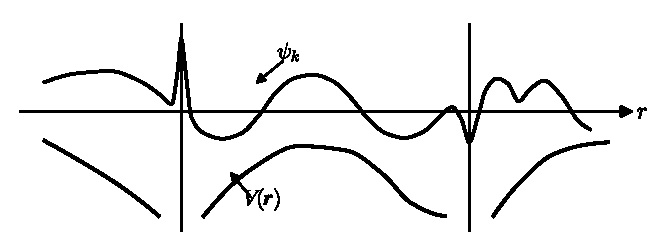
\includegraphics[width=7cm]{fig8-1.pdf}\\{\small 图 8.1\quad 布洛赫函数在离子实区的振荡特征}
\end{minipage}
\end{center}

表8.1\quad 由 $k=0$ W-S 元胞法波函数所算出的 Li 的 $a(\boldsymbol{K})$

\begin{center}\small
\begin{tabular}{ccc}
\hline
$|\boldsymbol{K}|$（以 $k_{\mathrm{F}}=0.589$ 原子单位量度） & 长度为 $|\boldsymbol{K}|$ 的倒格点个数 & $(N\Omega)^{1/2}a(\boldsymbol{K})$\\
\hline
0 & 1 & $-0.948$\\
1.353 & 12 & $+0.062$\\
1.914 & 6 & $+0.041$\\
2.344 & 24 & $+0.029$\\
2.706 & 12 & $+0.021$\\
3.026 & 24 & $+0.016$\\
3.315 & 8 & $+0.013$\\
3.580 & 48 & $+0.010$\\
3.828 & 6 & $+0.008$\\
4.060 & 36 & $+0.007$\\
4.279 & 24 & $+0.006$\\
4.488 & 24 & $+0.005$\\
$|\boldsymbol{K}|$（以 $k_{\mathrm{F}}=0.589$ 原子单位量度） & 长度为 $|\boldsymbol{K}|$ 的倒格点个数 & $(N\Omega)^{1/2}a(\boldsymbol{K})$\\
4.688 & 24 & $+0.004$\\
4.879 & 72 & $+0.004$\\
5.241 & 48 & $+0.003$\\
5.413 & 12 & $+0.003$\\
5.580 & 48 & $+0.002$\\
5.742 & 30 & $+0.002$\\
\hline
\end{tabular}
\end{center}

\section{正交化平面波法}

赫令（C.Herring）\textsuperscript{[2]}提出一种克服平面波展开收敛差的办法.首先将固体能带分为两类：壳层电子的能带和价带及导带，价带指的是最高的一个被占据能带，导带则代表最低的一个空（或半空）的能带.众所周知，费密面必然位于导带与价带附近，由于固体的特性主要由费密面附近电子的运动决定，所以人们感兴趣的是导带及价带结构.对于较低的壳层电子能带，一般都被填满，而且多半是窄能带，可以用紧束缚波函数表示为
\begin{equation}
  |\psi_{\mathrm{c}}\rangle=\frac{1}{\sqrt{N}}\sum_{\boldsymbol{l}}\mathrm{e}^{\mathrm{i}\boldsymbol{k}\cdot\boldsymbol{l}}|\phi_{\mathrm{c}}\rangle
\end{equation}
其中 $|\phi_{\mathrm{c}}\rangle$ 代表位于格点 $\boldsymbol{l}$ 上的原子波函数 $\phi_{\mathrm{c}}(\boldsymbol{r}-\boldsymbol{l})$，并假定为已知，它们满足本征方程
\begin{equation}
  H|\psi_{\mathrm{c}}\rangle=E_{\mathrm{c}}|\psi_{\mathrm{c}}\rangle
\end{equation}
当离子实体积很小，以致相邻格点的离子实波函数之间重叠可忽略时，$|\psi_{\mathrm{c}}\rangle$ 的表示式(8.2.1)就代表已归一化的壳层电子能带波函数，并满足条件
\begin{equation}
  \langle\psi_{\mathrm{c}'}|\psi_{\mathrm{c}}\rangle=\delta_{\mathrm{cc}'}
\end{equation}
其中 $\mathrm{c}$ 代表壳层态量子数，如1s，2p，….除贵金属与过渡金属外，对于单价及多价金属上述条件是合理的.例如，在铅（Pb）中 $1\mathrm{s}^{2}\cdots5\mathrm{s}^{2}5\mathrm{p}^{6}\mathrm{d}^{10}$ 代表离子实，$6\mathrm{s}^{2}6\mathrm{p}^{2}$ 为价电子态，其离子实的尺寸只有原子的一半，这时离子实只占总原子体积的1/8，故式(8.2.3)为合理的近似.

赫令注意到，对于固体中运动的电子，元胞中的离子实内区与离子实外区是两种性质上不同的区域.当导带或价带电子处于在离子实区以外时，仅受到弱势场作用，波函数在空间平滑变化，这时 $\psi_{\boldsymbol{k}}(\boldsymbol{r})$ 像平面波.在离子实区以内，由于有很强的局域势场作用，电子波函数表现出原子波函数的急剧振荡特征.因此最好采用平面波 $|\boldsymbol{k}+\boldsymbol{K}\rangle$ 与壳层能带波函数 $|\psi_{\mathrm{c}}\rangle$ 的某种线性组合来描述布洛赫函数，这样做才能兼顾两方面特征，应当说是更为切合实际情况的物理图像.
\begin{equation}
  |\psi_{\boldsymbol{k}}\rangle=\sum_{\boldsymbol{K}}\alpha(\boldsymbol{k}+\boldsymbol{K})|\boldsymbol{k}+\boldsymbol{K}\rangle+\sum_{\mathrm{c}}\beta_{\mathrm{c}}|\psi_{\mathrm{c}}\rangle
\end{equation}
系数 $\beta_{\mathrm{c}}$ 则由下面的正交化条件决定
\begin{equation}
  \langle\psi_{\mathrm{c}}|\psi_{\boldsymbol{k}}\rangle=0
\end{equation}
因为价带或导带的布洛赫函数与壳层能带波函数 $|\psi_{\mathrm{c}}\rangle$ 都是同一薛定谔方程不同本征值的解，它们理所当然的应当彼此正交.这个条件给出
\begin{equation}
  \beta_{\mathrm{c}}=-\sum_{\boldsymbol{K}}\alpha(\boldsymbol{k}+\boldsymbol{K})\langle\phi_{\mathrm{c}}|\boldsymbol{k}+\boldsymbol{K}\rangle
\end{equation}
由此求得导带及价带布洛赫函数的表示式：
\begin{equation}
\begin{aligned}
  |\phi_{\boldsymbol{k}}\rangle
  &=\sum_{\boldsymbol{K}}\alpha(\boldsymbol{k}+\boldsymbol{K})\Bigl[|\boldsymbol{k}+\boldsymbol{K}\rangle-\sum_{\mathrm{c}}|\phi_{\mathrm{c}}\rangle\langle\phi_{\mathrm{c}}|\boldsymbol{k}+\boldsymbol{K}\rangle\Bigr]\\
  &=\sum_{\boldsymbol{K}}\alpha(\boldsymbol{k}+\boldsymbol{K})|\mathrm{OPW}_{\boldsymbol{k}+\boldsymbol{K}}\rangle
\end{aligned}
\end{equation}
其中
\begin{equation}
  |\mathrm{OPW}_{\boldsymbol{k}}\rangle\equiv|\boldsymbol{k}\rangle-\sum_{\mathrm{c}}|\psi_{\mathrm{c}}\rangle\langle\psi_{\mathrm{c}}|\boldsymbol{k}\rangle
\end{equation}
称为正交化平面波（以下简称OPW），它是波矢为 $\boldsymbol{k}$ 的简单平面波与所有壳层能带的紧束缚波函数的特殊线性组合.组合结果必须与每一壳层能带波函数正交，即
\begin{equation}
  \langle\psi_{\mathrm{c}}|\mathrm{OPW}_{\boldsymbol{k}+\boldsymbol{K}}\rangle
  =\langle\psi_{\mathrm{c}}|\boldsymbol{k}+\boldsymbol{K}\rangle\Bigl(1-\sum_{\mathrm{c}'}\langle\psi_{\mathrm{c}}|\psi_{\mathrm{c}'}\rangle\Bigr)=0
\end{equation}
导（或价）带的布洛赫函数则是按正交化平面波 $|\mathrm{OPW}\rangle$ 展开表示的“傅里叶级数”，如式(8.2.7).将式(8.2.7)代入式(8.1.1)得
\begin{equation}
\begin{aligned}
  &(T+V-E)|\phi_{\boldsymbol{k}}\rangle\\
  &\quad=\sum_{\boldsymbol{K}}\alpha(\boldsymbol{k}+\boldsymbol{K})\bigl[(T+V-E)|\boldsymbol{k}+\boldsymbol{K}\rangle\\
  &\qquad-(T+V-E)\sum_{\mathrm{c}}|\phi_{\mathrm{c}}\rangle\langle\phi_{\mathrm{c}}|\boldsymbol{k}+\boldsymbol{K}\rangle\bigr]\\
  &\quad=0
\end{aligned}
\end{equation}
由于
\begin{equation}
  (T+V)|\psi_{\mathrm{c}}\rangle=E_{\mathrm{c}}|\psi_{\mathrm{c}}\rangle
\end{equation}
式(8.2.10)可写成
\begin{equation}
\begin{aligned}
  \sum_{\boldsymbol{K}}\alpha(\boldsymbol{k}+\boldsymbol{K})\biggl\{\Bigl[\frac{\hbar^{2}(\boldsymbol{k}+\boldsymbol{K})^{2}}{2m}-E\Bigr]|\boldsymbol{k}+\boldsymbol{K}\rangle+V|\boldsymbol{k}+\boldsymbol{K}\rangle\\
  +\sum_{\mathrm{c}}(E-E_{\mathrm{c}})|\phi_{\mathrm{c}}\rangle\langle\phi_{\mathrm{c}}|\boldsymbol{k}+\boldsymbol{K}\rangle\biggr\}=0
\end{aligned}
\end{equation}
将 $\langle\boldsymbol{k}+\boldsymbol{K}'|$ 作用于上式，求得 $\alpha$ 的线性方程组
\begin{equation}
\begin{aligned}
  \sum_{\boldsymbol{K}}\alpha(\boldsymbol{k}+\boldsymbol{K})\biggl\{\Bigl[\frac{\hbar^{2}(\boldsymbol{k}+\boldsymbol{K})^{2}}{2m}-E\Bigr]\delta_{\boldsymbol{K}\boldsymbol{K}'}\\
  +\langle\boldsymbol{k}+\boldsymbol{K}'|U|\boldsymbol{k}+\boldsymbol{K}\rangle\biggr\}=0
\end{aligned}
\end{equation}
其中矩阵元定义为
\begin{equation}
\begin{aligned}
  &\langle\boldsymbol{k}+\boldsymbol{K}'|U|\boldsymbol{k}+\boldsymbol{K}\rangle\\
  &\quad=\langle\boldsymbol{k}+\boldsymbol{K}'|V|\boldsymbol{k}+\boldsymbol{K}\rangle\\
  &\qquad+\sum_{\mathrm{c}}(E-E_{\mathrm{c}})\langle\boldsymbol{k}+\boldsymbol{K}'|\psi_{\mathrm{c}}\rangle\langle\psi_{\mathrm{c}}|\boldsymbol{k}+\boldsymbol{K}\rangle
\end{aligned}
\end{equation}
而决定能量本征值的久期方程为
\begin{equation}
\begin{aligned}
  \mathrm{det}\,\Bigl\|\Bigl[\frac{\hbar^{2}}{2m}(\boldsymbol{k}+\boldsymbol{K})^{2}-E\Bigr]\delta_{\boldsymbol{K}\boldsymbol{K}'}\\
  +\langle\boldsymbol{k}+\boldsymbol{K}'|U|\boldsymbol{k}+\boldsymbol{K}\rangle\Bigr\|=0
\end{aligned}
\end{equation}
这个行列式原则上也是无穷维的，但在实际应用中往往只需取少数几项就足够了.例如，对于锂（Li）只取展开式(8.2.7)中的一项（即一个正交化平面波），就能得出适用于价带的合理结果\textsuperscript{[3]}.应用为数不多的OPW作展开计算半导体锗 $(\mathrm{Ge})$\textsuperscript{[4]} 和硅 $(\mathrm{Si})$\textsuperscript{[5]} 的能带也取得了成功.比较图8.2中(a)平面波、(b)离子实波和(c)正交化平面波，可以看出一个OPW本身就包括了电子在离子实区的多次振荡特征.所以，一个OPW已经十分逼近真实波函数了，若进一步用OPW作展开表示 $\psi_{\boldsymbol{k}}$，其收敛必然比 $\psi_{\boldsymbol{k}}$ 平面波展开快得多.因此，OPW法是描述价带和导带电子波函数的好表象，是定量计算能带的一种重要方法.

关于OPW方法收敛性快的问题，还可以通过一个具体例子加以说明：例如计算金属锂的OPW矩阵元时，可取Li原子的1s态：
\begin{equation*}
\begin{aligned}
  &\phi_{\mathrm{c}}=\phi_{1\mathrm{s}}=\frac{\lambda^{3/2}}{\sqrt{\pi}}\exp(-\lambda r)
  \qquad\left(\lambda=2.37\,[\mathrm{a.u.}]^{-1}\right)\\
  &E_{\mathrm{c}}=E_{1\mathrm{s}}=-3.765\ [\mathrm{Ry}],\qquad V(\boldsymbol{r})=-\frac{e^{2}}{r}
\end{aligned}
\end{equation*}
则式(8.2.14)在 $\boldsymbol{K}'=\boldsymbol{0}$ 与 $E\approx\hbar^{2}k^{2}/2m$ 时可写为

\begin{center}
\begin{minipage}{7.5cm}
\centering
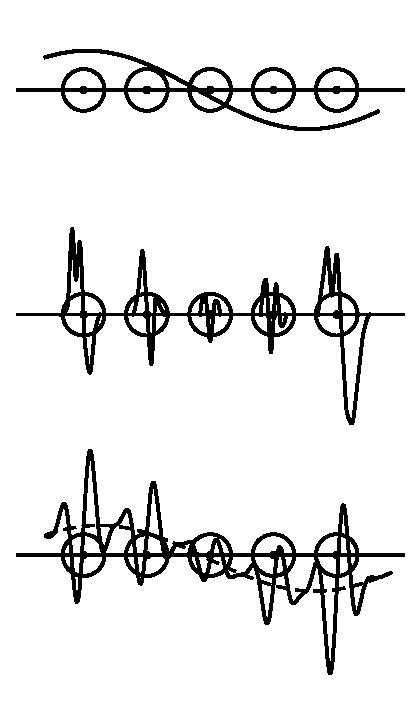
\includegraphics[width=7.5cm]{fig8-2.pdf}\\[0.3em]
{\small (a) 平面波\qquad\qquad (b) 离子实波\qquad\qquad (c) 正交化平面波}\\[0.2em]
{\small 图 8.2}
\end{minipage}
\end{center}

\begin{equation}
\begin{aligned}
  &\langle\boldsymbol{k}|U|\boldsymbol{k}+\boldsymbol{K}\rangle\\
  &\quad=\langle\boldsymbol{k}|V|\boldsymbol{k}+\boldsymbol{K}\rangle
  +\Bigl(\frac{\hbar^{2}k^{2}}{2m}+|E_{1\mathrm{s}}|\Bigr)
  \langle\boldsymbol{k}|\phi_{1\mathrm{s}}\rangle\langle\phi_{1\mathrm{s}}|\boldsymbol{k}+\boldsymbol{K}\rangle
\end{aligned}
\end{equation}
其中
\begin{equation*}
\begin{aligned}
  \langle\boldsymbol{k}|V|\boldsymbol{k}+\boldsymbol{K}\rangle
  &=\frac{1}{N\Omega}\int\mathrm{e}^{-\mathrm{i}\boldsymbol{k}\cdot\boldsymbol{r}}\Bigl(-\frac{e^{2}}{r}\Bigr)\mathrm{e}^{\mathrm{i}(\boldsymbol{k}+\boldsymbol{K})\cdot\boldsymbol{r}}\mathrm{d}\boldsymbol{r}\\
  &=\frac{1}{N\Omega}\int\Bigl(-\frac{e^{2}}{r}\Bigr)\mathrm{e}^{\mathrm{i}\boldsymbol{K}\cdot\boldsymbol{r}}\mathrm{d}\boldsymbol{r}
  =-\frac{4\pi e^{2}}{\Omega K^{2}}\\
  \langle\boldsymbol{k}|\psi_{1\mathrm{s}}\rangle
  &=\frac{1}{(N\Omega)^{1/2}}\int\mathrm{e}^{-\mathrm{i}\boldsymbol{k}\cdot\boldsymbol{r}}\psi_{1\mathrm{s}}(\boldsymbol{r})\mathrm{d}\boldsymbol{r}\\
  &=\frac{8\sqrt{\pi}}{(N\Omega)^{1/2}\lambda^{3/2}}\Bigl(1+\frac{k^{2}}{\lambda^{2}}\Bigr)^{-2}
\end{aligned}
\end{equation*}
求得OPW矩阵元
\begin{equation}
\begin{aligned}
  \langle\boldsymbol{k}|U|\boldsymbol{k}+\boldsymbol{K}\rangle
  &=-\frac{4\pi e^{2}}{N\Omega K^{2}}
  +\frac{64\pi}{N\Omega\lambda^{3}}
  \Bigl[\Bigl(1+\frac{k^{2}}{\lambda^{2}}\Bigr)
  \Bigl(1+\frac{|\boldsymbol{k}+\boldsymbol{K}|^{2}}{\lambda^{2}}\Bigr)\Bigr]^{-2}\times\\
  &\qquad\Bigl(\frac{\hbar^{2}k^{2}}{2m}+|E_{1\mathrm{s}}|\Bigr)
\end{aligned}
\end{equation}
上式右边第一项代表真实势 $V(\boldsymbol{r})$ 的矩阵元，第二项来源于正交化手续，它是一个正量，将对第一项起抵消作用，使 $\langle\boldsymbol{k}|U|\boldsymbol{k}+\boldsymbol{K}\rangle$ 成为比真实势弱的有效势矩阵元，从而有可能用低阶微扰处理OPW计算，自然其收敛性会比平面波法好.

\section{赝势方法}

已经看到，OPW方法中的正交化项起抵消势能的作用，并因此给出一个比真实势弱得多的有效势，试问能否在这种抵消作用的基础上发展一种计算导带和价带的新方案？赝势方法就是这样被提出来的.

\subsection*{1. OPW赝势}

将布洛赫函数的OPW展开式(8.2.7)写为
\begin{equation}
  |\psi_{\boldsymbol{k}}\rangle=|\chi_{\boldsymbol{k}}\rangle-\sum_{\mathrm{c}}|\psi_{\mathrm{c}}\rangle\langle\psi_{\mathrm{c}}|\chi_{\boldsymbol{k}}\rangle
\end{equation}
这里引进一个新函数
\begin{equation}
  |\chi_{\boldsymbol{k}}\rangle=\sum_{\boldsymbol{K}}\alpha(\boldsymbol{k}+\boldsymbol{K})|\boldsymbol{k}+\boldsymbol{K}\rangle
\end{equation}
并设其中的展开系数与OPW展开式(8.2.7)中的 $\alpha(\boldsymbol{k}+\boldsymbol{K})$ 相同.为说明这样组合的简单平面波的特征，先讨论 $|\chi_{\boldsymbol{k}}\rangle$ 满足什么方程.

将 $|\psi_{\boldsymbol{k}}\rangle$ 代入薛定谔方程
\begin{equation}
  H|\psi_{\boldsymbol{k}}\rangle=E_{k}|\psi_{\boldsymbol{k}}\rangle
\end{equation}
得
\begin{equation}
  H|\chi_{\boldsymbol{k}}\rangle-\sum_{\mathrm{c}}\langle\psi_{\mathrm{c}}|\chi_{\boldsymbol{k}}\rangle H|\psi_{\mathrm{c}}\rangle
  =E_{k}|\chi_{\boldsymbol{k}}\rangle-E_{k}\sum_{\mathrm{c}}\langle\psi_{\mathrm{c}}|\chi_{\boldsymbol{k}}\rangle|\psi_{\mathrm{c}}\rangle
\end{equation}
利用
\begin{equation}
  H|\psi_{\mathrm{c}}\rangle=E_{\mathrm{c}}|\psi_{\mathrm{c}}\rangle
\end{equation}
可求得 $|\chi_{\boldsymbol{k}}\rangle$ 的方程式
\begin{equation}
  H|\chi_{\boldsymbol{k}}\rangle+\sum_{\mathrm{c}}(E_{k}-E_{\mathrm{c}})|\psi_{\mathrm{c}}\rangle\langle\psi_{\mathrm{c}}|\chi_{\boldsymbol{k}}\rangle=E_{k}|\chi_{\boldsymbol{k}}\rangle
\end{equation}
再利用式(8.1.1)写为
\begin{equation}
  (T+U)|\chi_{\boldsymbol{k}}\rangle=E_{k}|\chi_{\boldsymbol{k}}\rangle
\end{equation}
其中
\begin{equation}
  U|\chi_{\boldsymbol{k}}\rangle=V|\chi_{\boldsymbol{k}}\rangle
  +\sum_{\mathrm{c}}(E_{k}-E_{\mathrm{c}})|\psi_{\mathrm{c}}\rangle\langle\psi_{\mathrm{c}}|\chi_{\boldsymbol{k}}\rangle
\end{equation}
$U=V+\sum_{\mathrm{c}}(E_{k}-E_{\mathrm{c}})|\psi_{\mathrm{c}}\rangle\langle\psi_{\mathrm{c}}|$ 称为赝势，而 $|\chi_{\boldsymbol{k}}\rangle$ 是在赝势作用下运动的电子波函数，人们称之为赝波函数.比较式(8.3.3)和(8.3.7)可知，赝波函数 $|\chi_{\boldsymbol{k}}\rangle$ 与布洛赫函数 $|\psi_{\boldsymbol{k}}\rangle$ 具有完全相同的能量本征值 $E_{k}$，这是赝势方法的重要特点.现在分析赝势的大小，注意到 $E_{k}$ 为导（或价）带中电子能量，显然它应当大于壳层态中的电子能量 $E_{\mathrm{c}}$，使 $U$ 中第二项的贡献为正.所以，赝势中正交化所带来的是一个排斥势，它与真实的吸引势有相消趋势.从物理上看，要求价电子态与被填满的离子实轨道态正交相当于泡利不相容原理，而正交性要求必然使价电子波函数在离子实区引进振荡\footnote{因为离子实中壳层电子波函数是振荡的，价电子波函数也必须在离子实区内振荡，否则两者不能正交.}.这种急剧振荡又将使价电子产生高平均动能，并对离子实区的强吸引势起抵消作用，因此价电子实际上只受到弱的净势作用，相当于一个微扰势，这就是赝势.当我们用赝势取代真实势解薛定谔方程时，相应的赝波函数也就没有复杂的振荡特征了.

综上所述，从OPW出发，我们可以找到一个赝波动方程(8.3.7)，它与严格布洛赫函数的能量本征值相同，但赝势和赝波函数相对于真实势和严格波函数都是被平滑化了的，所以组合少数平面波就足以描述赝波函数的展式(8.3.2)了.因此，计算能带时不必先求布洛赫函数，可直接从式(8.3.8)出发，先计算赝势，然后用赝波动方程(8.3.7)求解平滑函数所对应的能量 $E_{k}$ 值，这就是建立在OPW基础上的赝势方法，它原则上等同于作OPW计算，因为在这里要求式(8.2.7)与(8.3.2)的展开系数 $\alpha(\boldsymbol{k}+\boldsymbol{K})$ 相同.

\subsection*{2. 赝势法的非唯一性特征}

赝势法的优点不仅如此.现在我们将超出OPW的范围，更一般地讨论赝势法.

一般赝势法原则上也是利用价带或导带电子波函数与离子实电子波函数正交的事实.从布洛赫函数的薛定谔方程出发
\begin{equation*}
  (T+V)|\psi_{\boldsymbol{k}}\rangle=E_{k}|\psi_{\boldsymbol{k}}\rangle
\end{equation*}
利用正交条件 $\langle\psi_{\mathrm{c}}|\psi_{\boldsymbol{k}}\rangle=0$，得到形式上与式(8.3.1)相同的表示式
\begin{equation}
  |\psi_{\boldsymbol{k}}\rangle=|\chi_{\boldsymbol{k}}\rangle-\sum_{\mathrm{c}}|\psi_{\mathrm{c}}\rangle\langle\psi_{\mathrm{c}}|\chi_{\boldsymbol{k}}\rangle
\end{equation}
这里 $|\chi_{\boldsymbol{k}}\rangle$ 是一般的赝波函数.它满足赝波动方程（赝势方程）
\begin{equation}
  (T+U)|\chi_{\boldsymbol{k}}\rangle=E_{k}|\chi_{\boldsymbol{k}}\rangle
\end{equation}
其中
\begin{equation}
  U|\chi_{\boldsymbol{k}}\rangle=V|\chi_{\boldsymbol{k}}\rangle
  +\sum_{\mathrm{c}}(E_{k}-E_{\mathrm{c}})|\phi_{\mathrm{c}}\rangle\langle\phi_{\mathrm{c}}|\chi_{\boldsymbol{k}}\rangle
\end{equation}
试问 $|\chi_{\boldsymbol{k}}\rangle$ 有何特性？不难看出，若将壳层波函数的任意线性组合附加于 $|\chi_{\boldsymbol{k}}\rangle$，则新赝波函数
\begin{equation}
  |\chi'_{\boldsymbol{k}}\rangle=|\chi_{\boldsymbol{k}}\rangle+\sum_{\mathrm{c}'}\gamma_{\mathrm{c}'}|\psi_{\mathrm{c}'}\rangle
\end{equation}
满足同样的赝波动方程：
\begin{equation}
\begin{aligned}
  (T+U)|\chi'_{\boldsymbol{k}}\rangle
  &=(T+U)|\chi_{\boldsymbol{k}}\rangle+(T+U)\sum_{\mathrm{c}'}\gamma_{\mathrm{c}'}|\psi_{\mathrm{c}'}\rangle\\
  &=E_{k}|\chi_{\boldsymbol{k}}\rangle+H\sum_{\mathrm{c}'}\gamma_{\mathrm{c}'}|\psi_{\mathrm{c}'}\rangle+(U-V)\sum_{\mathrm{c}'}\gamma_{\mathrm{c}'}|\psi_{\mathrm{c}'}\rangle\\
  &=E_{k}|\chi_{\boldsymbol{k}}\rangle+\sum_{\mathrm{c}'}\gamma_{\mathrm{c}'}E_{\mathrm{c}'}|\psi_{\mathrm{c}'}\rangle
  +\sum_{\mathrm{c}',\mathrm{c}}\gamma_{\mathrm{c}'}(E_{k}-E_{\mathrm{c}})|\psi_{\mathrm{c}}\rangle\langle\psi_{\mathrm{c}}|\psi_{\mathrm{c}'}\rangle\\
  &=E_{k}\Bigl(|\chi_{\boldsymbol{k}}\rangle+\sum_{\mathrm{c}'}\gamma_{\mathrm{c}'}|\psi_{\mathrm{c}'}\rangle\Bigr)\\
  &=E_{k}|\chi'_{\boldsymbol{k}}\rangle
\end{aligned}
\end{equation}
以上结果说明：当 $|\chi_{\boldsymbol{k}}\rangle$ 是赝势方程的解时，$|\chi'_{\boldsymbol{k}}\rangle$ 也是此方程同一本征值 $E_{k}$ 的解，这就是赝波动方程解的非唯一性特征.在推导式(8.3.13)时，利用了 $\langle\psi_{\mathrm{c}}|\psi_{\mathrm{c}'}\rangle=\delta_{\mathrm{cc}'}$.

与此相应，赝势 $U$ 的选取也是非唯一的.1962年奥斯丁（Austin）等人\textsuperscript{[6]}指出，利用正交条件 $\langle\psi_{\boldsymbol{k}}|\psi_{\mathrm{c}}\rangle=0$，由式(8.3.11)可求出赝势条件
\begin{equation}
  \langle\psi_{\boldsymbol{k}}|(U-V)|\chi_{\boldsymbol{k}}\rangle=0
\end{equation}
满足这个条件的一般赝势为
\begin{equation}
  U|\chi_{\boldsymbol{k}}\rangle=V|\chi_{\boldsymbol{k}}\rangle+\sum_{\mathrm{c}}|\psi_{\mathrm{c}}\rangle\langle\psi_{\mathrm{c}}|F|\chi_{\boldsymbol{k}}\rangle
\end{equation}
其中 $F$ 为任意算子，因为 $\langle\psi_{\boldsymbol{k}}|\psi_{\mathrm{c}}\rangle=0$ 可保证以上赝势 $U$ 仍满足式(8.3.14)，按式(8.3.15)决定的 $U$ 称为广义赝势.在式(8.3.15)中若取 $F=0$，将回到布洛赫波函数的薛定谔方程，若取 $F=E_{k}-H$，则是OPW赝势方程(8.3.8).由此可知，赝势的选择也不是唯一的.对于导带或价带电子，凡满足式(8.3.14)的任何赝势都给出相同的能量本征值 $E_{k}$.

非唯一性是赝势法的固有特性，利用它可选定最佳赝势使赝波函数尽可能平滑.在具体计算时，可利用变分技巧，要求赝势尽可能小，从而决定 $\langle\psi_{\mathrm{c}}|F|\chi_{\boldsymbol{k}}\rangle$，或者从赝波函数尽可能是空间缓慢变化的要求确定系数 $\gamma_{\mathrm{c}'}$，这两种要求大体上是等效的.按此选定的赝波函数可近似由少数平面波叠加构成，这是赝势方法的核心.

总之，赝势的引入将 $H=T+V$ 换成 $H_{\mathrm{ps}}=T+U$，可以求出与 $H$ 一样的本征值 $E_{k}$，但其波函数 $\chi_{k}$ 已是空间的缓变函数，可以用平面波作为良好近似，并将使能谱的求解大为简化.

\subsection*{3. 赝势计算方案}

若将 $|\chi_{\boldsymbol{k}}\rangle$ 展开为平面波，可求得与§1中相同的久期方程，只不过真实势 $V$ 的矩阵元 $\langle\boldsymbol{k}'+\boldsymbol{K}'|V|\boldsymbol{k}+\boldsymbol{K}\rangle$ 换成了赝势 $U$ 的矩阵元.困难在于 $U$ 是非定域势（即积分算子），假如近似用一个定域的赝势 $U(\boldsymbol{r})$ 来描述，则
\begin{equation}
  \langle\boldsymbol{k}+\boldsymbol{K}'|U|\boldsymbol{k}+\boldsymbol{K}\rangle
  =\frac{1}{N\Omega}\int U(\boldsymbol{r})\mathrm{e}^{-\mathrm{i}\boldsymbol{q}\cdot\boldsymbol{r}}\mathrm{d}\boldsymbol{r}
  \qquad(\boldsymbol{q}=\boldsymbol{K}'-\boldsymbol{K})
\end{equation}
将 $U(\boldsymbol{r})$ 用各离子赝势之和表示，对于每个元胞中含多个原子的复式晶格情况，得到
\begin{equation}
  U(\boldsymbol{r})=\sum_{\alpha,\,\boldsymbol{l}}v_{\alpha}(\boldsymbol{r}-\boldsymbol{l}-\boldsymbol{R}_{\alpha})
\end{equation}
其中 $v_{\alpha}$ 代表元胞中第 $\alpha$ 个离子的势能，$\boldsymbol{R}_{\alpha}$ 为其在元胞中的位置矢.$U(\boldsymbol{r})$ 的傅里叶分量为
\begin{equation}
\begin{aligned}
  U(\boldsymbol{q})&=\langle\boldsymbol{k}+\boldsymbol{K}'|U|\boldsymbol{k}+\boldsymbol{K}\rangle\\
  &=\frac{1}{N\Omega}\sum_{\alpha,\,\boldsymbol{l}}\int v_{\alpha}(\boldsymbol{r}-\boldsymbol{l}-\boldsymbol{R}_{\alpha})\mathrm{e}^{-\mathrm{i}\boldsymbol{q}\cdot\boldsymbol{r}}\mathrm{d}\boldsymbol{r}\\
  &=\frac{1}{\Omega}\sum_{\alpha}\mathrm{e}^{-\mathrm{i}\boldsymbol{q}\cdot\boldsymbol{R}_{\alpha}}\int v_{\alpha}(\boldsymbol{r})\mathrm{e}^{-\mathrm{i}\boldsymbol{q}\cdot\boldsymbol{r}}\mathrm{d}\boldsymbol{r}\\
  &=\sum_{\alpha}\mathrm{e}^{-\mathrm{i}\boldsymbol{q}\cdot\boldsymbol{R}_{\alpha}}I_{\alpha}
\end{aligned}
\end{equation}
其中
\begin{equation}
  I_{\alpha}\equiv\frac{1}{\Omega}\int v_{\alpha}(\boldsymbol{r})\mathrm{e}^{-\mathrm{i}\boldsymbol{q}\cdot\boldsymbol{r}}\mathrm{d}\boldsymbol{r}
\end{equation}
叫形状因子.对于全同原子组成的晶体，$I_{\alpha}$ 与 $\alpha$ 无关，这时
\begin{equation}
  U(\boldsymbol{q})=I\sum_{\alpha}\mathrm{e}^{-\mathrm{i}\boldsymbol{q}\cdot\boldsymbol{R}_{\alpha}}\equiv IS(\boldsymbol{q})
\end{equation}
$S(\boldsymbol{q})$ 称为结构因子.当所选赝势足够平滑时，$U(\boldsymbol{q})$ 中只有小 $\boldsymbol{q}$ 值的傅里叶分量是重要的，这时久期行列式的维数变得很小，只要已知形状因子 $I_{\alpha}$，能带结构就不难算出.在定量计算时，$I_{\alpha}$ 由实验值确定.

还可以利用赝势的非唯一性，把离子实区的赝势取得尽量简单，并引进一组可调参量，最后由匹配条件决定这些参量，以保证在离子实区以外 $|\chi_{\boldsymbol{k}}\rangle$ 与 $|\psi_{\boldsymbol{k}}\rangle$ 一致.例如，海因（Heine）等人\textsuperscript{[7]}将离子的真实势在离子实区用一个方阱模型代替（如图8.3所示）.
\begin{equation}
  U_{\mathrm{M}}=\begin{cases}
    -A_{l} & (\boldsymbol{r}\leqslant\boldsymbol{a}_{\mathrm{M}})\\[0.2em]
    -\dfrac{Ze^{2}}{r} & (\boldsymbol{r}>\boldsymbol{a}_{\mathrm{M}})
  \end{cases}
\end{equation}
其中 $Z$ 为化学价，$A_{l}$ 为阱深，它与壳层态量子数 $l$ 有关.调节参数 $A_{l}$ 与 $a_{\mathrm{M}}$，可使模型赝势的波动方程解与观测的自由原子光谱项一致，这种办法很成功地用于原子问题，避免了解自洽方程的麻烦.当用于固体时，设在 $r\leqslant a_{\mathrm{M}}$ 时赝势为 $-A(E)$，在最简单情况下可令它等于零，而可调参量 $a_{\mathrm{M}}$ 则由 $r=a_{\mathrm{M}}$ 处赝波函数与布洛赫函数相等条件决定.图8.4对晶体的真实势和赝势以及布洛赫函数和赝波函数作了比较.

\begin{center}
\begin{minipage}{6.5cm}
\centering
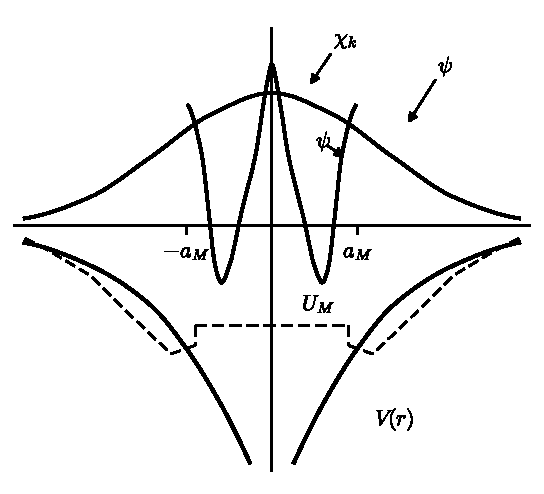
\includegraphics[width=6.5cm]{fig8-3.pdf}\\{\small 图 8.3\quad 用于离子的模型赝势}
\end{minipage}
\end{center}

\begin{center}
\begin{minipage}{8cm}
\centering
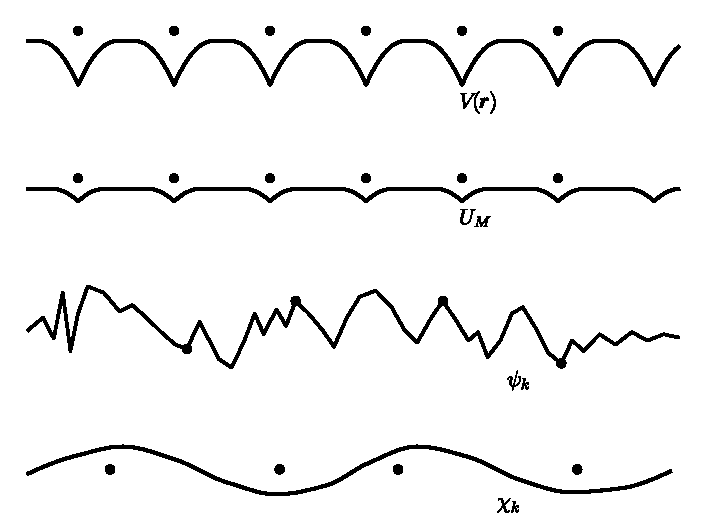
\includegraphics[width=8cm]{fig8-4.pdf}\\[0.3em]
{\small (a) 晶体势 $V(\boldsymbol{r})$\qquad\qquad (b) 赝势 $U_{\mathrm{M}}$}\\[0.2em]
{\small (c) 布洛赫函数 $\psi_{\boldsymbol{k}}$\qquad\qquad (d) 赝波函数 $\chi_{\boldsymbol{k}}$}\\[0.2em]
{\small 图 8.4\quad 晶体中模型赝势的示意图}
\end{minipage}
\end{center}
\section{近自由电子方法的赝势证明}

引入赝势的另一重要成就是：证明了近自由电子方法适用于离子实半径小的金属能带计算，其证明如下.

鉴于赝波函数的非唯一性，我们希望能找到一个平滑的 $\chi_{\boldsymbol{k}}$，显然其选择条件要求下列量
\begin{equation}
  \frac{\int|\nabla\chi_{\boldsymbol{k}}|^{2}\,\mathrm{d}\tau}{\int|\chi_{\boldsymbol{k}}|^{2}\,\mathrm{d}\tau}
\end{equation}
为极小，此要求等效于动能极小条件，因为
\begin{equation}
\begin{aligned}
  \int|\nabla\chi_{\boldsymbol{k}}|^{2}\,\mathrm{d}\tau
  &=\int\nabla\chi_{\boldsymbol{k}}^{*}\cdot\nabla\chi_{\boldsymbol{k}}\,\mathrm{d}\tau\\
  &=\int_{S}(\chi_{\boldsymbol{k}}^{*}\nabla\chi_{\boldsymbol{k}})\cdot\mathrm{d}\boldsymbol{S}
  -\int\chi_{\boldsymbol{k}}^{*}\nabla^{2}\chi_{\boldsymbol{k}}\,\mathrm{d}\tau
\end{aligned}
\end{equation}
由于周期性边界条件，上式右边的面积分项为零，而第二项正比于动能.所以，可利用动能极小条件选择最佳的 $\chi_{\boldsymbol{k}}$，设
\begin{equation}
  \overline{T}=\frac{\langle\chi_{\boldsymbol{k}}|T|\chi_{\boldsymbol{k}}\rangle}{\langle\chi_{\boldsymbol{k}}|\chi_{\boldsymbol{k}}\rangle}
\end{equation}
则其变分方程为
\begin{equation}
  \langle\delta\chi|T|\chi_{\boldsymbol{k}}\rangle-\overline{T}\langle\delta\chi|\chi_{\boldsymbol{k}}\rangle=0
\end{equation}
按照赝波函数的非唯一性，取 $|\delta\chi\rangle=\sum_{\mathrm{c}}\gamma_{\mathrm{c}}|\psi_{\mathrm{c}}\rangle$，得到
\begin{equation}
  \langle\psi_{\mathrm{c}}|T|\chi_{\boldsymbol{k}}\rangle-\overline{T}\langle\psi_{\mathrm{c}}|\chi_{\boldsymbol{k}}\rangle=0
\end{equation}
由此求得
\begin{equation}
  \langle\psi_{\mathrm{c}}|(E_{k}-T)|\chi_{\boldsymbol{k}}\rangle
  =(E_{k}-\overline{T})\langle\psi_{\mathrm{c}}|\chi_{\boldsymbol{k}}\rangle
\end{equation}
将上式代入广义赝势的表示式(8.3.15)并取 $F=E_{k}-H$
\begin{equation}
\begin{aligned}
  U|\chi_{\boldsymbol{k}}\rangle
  &=V|\chi_{\boldsymbol{k}}\rangle+\sum_{\mathrm{c}}|\psi_{\mathrm{c}}\rangle\langle\psi_{\mathrm{c}}|F|\chi_{\boldsymbol{k}}\rangle\\
  &=V|\chi_{\boldsymbol{k}}\rangle+\sum_{\mathrm{c}}|\psi_{\mathrm{c}}\rangle\langle\psi_{\mathrm{c}}|(E_{k}-H)|\chi_{\boldsymbol{k}}\rangle\\
  &=V|\chi_{\boldsymbol{k}}\rangle+\sum_{\mathrm{c}}|\psi_{\mathrm{c}}\rangle\langle\psi_{\mathrm{c}}|(E_{k}-T)|\chi_{\boldsymbol{k}}\rangle\\
  &\qquad-\sum_{\mathrm{c}}|\psi_{\mathrm{c}}\rangle\langle\psi_{\mathrm{c}}|V|\chi_{\boldsymbol{k}}\rangle\\
  &=V|\chi_{\boldsymbol{k}}\rangle-\sum_{\mathrm{c}}|\psi_{\mathrm{c}}\rangle\langle\psi_{\mathrm{c}}|V|\chi_{\boldsymbol{k}}\rangle\\
  &\qquad+(E_{k}-\overline{T})\sum_{\mathrm{c}}|\psi_{\mathrm{c}}\rangle\langle\psi_{\mathrm{c}}|\chi_{\boldsymbol{k}}\rangle
\end{aligned}
\end{equation}
注意，上式右边第三项经 $\langle\chi_{\boldsymbol{k}}|$ 作用后变为
\begin{equation}
  \sum_{\mathrm{c}}|\langle\psi_{\mathrm{c}}|\chi_{\boldsymbol{k}}\rangle|^{2}
  =\sum_{\mathrm{c}}\langle\chi_{\boldsymbol{k}}|\psi_{\mathrm{c}}\rangle\langle\psi_{\mathrm{c}}|\chi_{\boldsymbol{k}}\rangle
  =\frac{\Delta}{\Omega}
\end{equation}
其中 $\Omega$ 为元胞体积，赝波函数可近似取 $\dfrac{1}{\sqrt{\Omega}}\mathrm{e}^{\mathrm{i}\boldsymbol{k}\cdot\boldsymbol{r}}$，并设壳层电子波函数在离子实区体积 $\Delta$ 之外近似为零.对于 $\dfrac{\Delta}{\Omega}$ 为小量的金属，式(8.4.8)右边近似等于零.这时式(8.4.7)等式右边第三项可忽略不计，由此求得关系式
\begin{equation}
  U|\chi_{\boldsymbol{k}}\rangle\approx V|\chi_{\boldsymbol{k}}\rangle
  -\sum_{\mathrm{c}}|\psi_{\mathrm{c}}\rangle\langle\psi_{\mathrm{c}}|V|\chi_{\boldsymbol{k}}\rangle
\end{equation}
再用 $\langle\psi_{\mathrm{c}}|$ 作用于上式，得到
\begin{equation}
  \langle\psi_{\mathrm{c}}|U|\chi_{\boldsymbol{k}}\rangle\approx 0
\end{equation}
此结果说明，在离子实区赝势几乎完全抵消.本来处理价电子问题的麻烦就在于离子实区晶体势很强，采用平面波法严格求解布洛赫函数不方便，从而怀疑近自由电子法已成功求出的能谱.现已明白，近自由电子方法相当于作某种赝势计算，而不必要求赝波函数在离子实区与真实布洛赫函数一致.这就为近自由电子方法用于金属导带及价带能谱计算提供了有力的理论根据.20世纪60年代初，正由于赝势理论的发展，哈里逊（Harrison）在近似自由电子法基础上提出了费密面构造法，对一系列金属给出了有用的费密面构型\textsuperscript{[8]}.但是，这种方法只适用于非过渡金属和非贵金属.对于过渡金属和贵金属，其离子实半径较大，上述证明失效.这时必须用更精确的能带计算方法，例如§6中的缀加平面波法.
\section{元胞法}

元胞法是维格纳和赛茨于1933年\textsuperscript{[9]}研究碱金属结合能时提出的，适合于单价金属导带的最低能量状态计算，它是历史上第一个定量计算能带的方法.下面将以简单晶格（每个元胞中只含一个原子）为例，介绍元胞法.

以某原子为中心，作该原子与近邻以及次近邻原子连线的垂直平分面，由这些平面所围成的多面体即W-S元胞，它的体积与正点阵的初基元胞体积相等，整个晶体可以看作是由各原子的W-S元胞堆积而成的.bcc晶格的W-S元胞是截角八面体，fcc晶格的W-S元胞为菱十二面体，它们都是对称化的多面体，并且充分反映了晶格的点群对称性.因此，在对称化元胞面上给予适当的边界条件，可将能带计算问题简化为在一个W-S元胞内求解薛定谔方程问题，即
\begin{equation}
  -\frac{\hbar^{2}}{2m}\nabla^{2}\psi_{\boldsymbol{k}}(\boldsymbol{r})
  +V(\boldsymbol{r})\psi_{\boldsymbol{k}}(\boldsymbol{r})=E_{k}\psi_{\boldsymbol{k}}(\boldsymbol{r})
\end{equation}
要求波函数 $\psi_{\boldsymbol{k}}$ 及其导数在W-S多面体上任一点 $\boldsymbol{r}=\boldsymbol{R}_{\mathrm{b}}$ 为连续，加上布洛赫定理 $\psi_{\boldsymbol{k}}(\boldsymbol{r}+\boldsymbol{l})=\mathrm{e}^{\mathrm{i}\boldsymbol{k}\cdot\boldsymbol{l}}\psi_{\boldsymbol{k}}(\boldsymbol{r})$，给出元胞法的边界条件：
\begin{equation}
  \psi_{\boldsymbol{k}}(\boldsymbol{R}_{\mathrm{b}}+\boldsymbol{l})
  =\exp(\mathrm{i}\boldsymbol{k}\cdot\boldsymbol{l})\psi_{\boldsymbol{k}}(\boldsymbol{R}_{\mathrm{b}})
\end{equation}
\begin{equation}
  \nabla_{n}\psi_{\boldsymbol{k}}(\boldsymbol{R}_{\mathrm{b}}+\boldsymbol{l})
  =-\exp(\mathrm{i}\boldsymbol{k}\cdot\boldsymbol{l})\nabla_{n}\psi_{\boldsymbol{k}}(\boldsymbol{R}_{\mathrm{b}})
\end{equation}
式(8.5.3)中负号是由于 $\boldsymbol{R}_{\mathrm{b}}$ 点与 $\boldsymbol{R}_{\mathrm{b}}+\boldsymbol{l}$ 点所在面的法线取向相反.如果在W-S元胞面上所有点均满足条件，则方程(8.5.1)在元胞内的解必然是能量为 $E_{k}$ 波矢为 $\boldsymbol{k}$ 的布洛赫函数.到此为止，我们还未作任何近似，仅仅是从整个晶体的求解变换为在W-S元胞中的计算.

元胞法的基本近似是假定在W-S元胞内晶体势场具有球对称性
\begin{equation}
  V(\boldsymbol{r})=V(r)
\end{equation}
因此在元胞内薛定谔方程可通过分离变量法求解，用球谐函数 $\mathrm{Y}_{lm}(\theta,\phi)$ 与径向函数 $R_{l}(E_{k},r)$ 之乘积将能带中 $\boldsymbol{k}$ 状态的波函数表示为
\begin{equation}
  \psi_{\boldsymbol{k}}(\boldsymbol{r})=\sum_{l,\,m}b_{lm}(\boldsymbol{k})\mathrm{Y}_{lm}(\theta,\phi)R_{l}(E_{k},r)
\end{equation}
其中径向函数满足微分方程
\begin{equation}
  \frac{1}{r^{2}}\frac{\mathrm{d}}{\mathrm{d}r}\Bigl(r^{2}\frac{\mathrm{d}R_{l}}{\mathrm{d}r}\Bigr)
  +\Bigl[\frac{2m}{\hbar^{2}}\bigl(E-V(r)\bigr)-\frac{l(l+1)}{r^{2}}\Bigr]R_{l}=0
\end{equation}
若 $V(r)$ 已知，则对于任意给定的 $E_{k}$ 值，可求出 $R_{l}\ (l=0,1,2,\cdots)$ 的数值解.在波函数的展开式(8.5.5)中未知系数 $b_{lm}$ 应由边界条件决定.对于给定的 $\boldsymbol{k}$，只有特殊的 $E_{k}$ 值可选择系数 $b_{lm}$ 使 $\psi_{\boldsymbol{k}}$ 满足式(8.5.2)和(8.5.3).因此，在确定 $b_{lm}$ 的同时，也定出了能量本征值 $E_{k}$.换句话说，当要求 $\psi_{\boldsymbol{k}}$ 在W-S元胞面上满足边界条件时，我们将求得一组以 $b_{lm}$ 为未知量的线性齐次方程，而 $E_{k}$ 应根据 $b_{lm}$ 的非零解条件（即 $b_{lm}$ 的系数行列式等于零）决定.

应当注意，只有在球形势近似下才能得到径向波函数 $R_{l}$ 的单独方程(8.5.6).如果在 $V(r)$ 中包含了非球对称项，并将它按球函数展开，那时将会得到不同 $l$ 的径向函数彼此耦合的联立微分方程组，对它作计算将是十分复杂的.因此，只有当球形势近似成立时，元胞法才是实用的.从多体理论的观点来讲，由于自旋平行的公有化电子间的交换作用以及反平行自旋电子间的关联作用，在每个电子周围将排开其它电子，并且可以近似认为每个W-S元胞内只含一个电子.这个电子将受到：(i)来自元胞内离子实的作用，它是有心力场.(ii)来自其它 $(N-1)$ 个元胞中离子实与电子的作用.由于每个W-S元胞整体呈电中性，来自其它元胞的作用在低阶近似下可以忽略不计.因此，只剩下元胞内离子实对电子的作用，它显然是球形对称的势场.在高阶近似下，还应当考虑来自其它元胞的多极势作用，其影响主要在W-S元胞边界附近，对于碱金属（如Na），维格纳和赛茨\textsuperscript{[9]}的计算证实，多极势对静电能的修正可忽略不计，说明对于碱金属采用球形势近似是合理的.

由于在式(8.5.5)中对 $l$、$m$ 的求和可以到无限，在 $\psi_{\boldsymbol{k}}$ 的展开式中应有无限多个未知系数 $b_{lm}$，要求我们在W-S元胞界面上取无限个点作为边界条件来确定未知系数.这当然只是原则精神，实际运算时，只能将 $\psi_{\boldsymbol{k}}$ 的展开式(8.5.5)在某个 $l$ 值处作切断，只取有限项.但是，要得到较精确的解，必须在较大的 $l$ 值上切断，则式(8.5.5)中仍含有许多项.这时利用晶体对称性可使问题简化，特别是对于BZ中的高对称点，可以利用波函数的已知对称特性，消去展开式(8.5.5)中许多球谐函数项，以至于所取切断 $l$ 值尽管较大，但只涉及少数未知系数的计算.这里要用群论来改组展开式(8.5.5)，因为在W-S元胞面上的边界条件是具有晶体点群对称性的.但是，波函数 $\psi_{\boldsymbol{k}}$ 的展开式中的球函数 $\mathrm{Y}_{lm}$ 只具有旋转群变换的特征，还必须将球谐函数作某种线性组合，才能使 $\psi_{\boldsymbol{k}}$ 的变换性质与 $\boldsymbol{k}$ 波矢群的不可约表示相符合，从而使 $\psi_{\boldsymbol{k}}$ 的表示式反映晶格的点群对称性.因此，将式(8.5.5)改写成
\begin{equation}
  \psi_{\boldsymbol{k}}(\boldsymbol{r})=\sum_{l}A_{l}(\boldsymbol{k})\Bigl[\sum_{m}C_{lm}(\boldsymbol{k})\mathrm{Y}_{lm}(\theta,\phi)\Bigr]R_{l}(E_{k},\boldsymbol{r})
\end{equation}
其中 $\sum_{m}C_{lm}(\boldsymbol{k})\mathrm{Y}_{lm}(\theta,\phi)$ 称为晶格谐函数（lattice harmonics）.对于立方晶格的BZ中的高对称点和对称线上的晶格谐函数均可查表求得\textsuperscript{[10]}，这是元胞法的优点.对于碱金属在BZ中心点（$\boldsymbol{k}=0$ 处）的波函数，维格纳和赛茨采用合理的近似，得到了极其简单的计算公式.

\subsection*{1. 维格纳-赛茨的计算}

在 $\boldsymbol{k}=0$ 点，边界条件式(8.5.2)和式(8.5.3)简化为波函数 $\psi_{0}\equiv\psi_{\boldsymbol{k}=0}$ 在W-S元胞面上的法向导数等于零：
\begin{equation}
  \nabla_{n}\psi_{0}(\boldsymbol{R}_{\mathrm{b}})=0
\end{equation}
$\psi_{0}$ 是正点阵的周期函数.维格纳-赛茨指出，由于W-S元胞多面体的高度对称性，可以把W-S元胞近似当作半径为 $r_{\mathrm{s}}$ 的球，其体积与元胞相同.对于bcc晶格，$r_{\mathrm{s}}$ 为
\begin{equation}
  \frac{4\pi}{3}r_{\mathrm{s}}^{3}=\frac{1}{2}a^{3}\qquad(r_{\mathrm{s}}\approx 0.49a)
\end{equation}
其中 $a$ 代表立方胞边长.这时 $\boldsymbol{k}=0$ 处的最低能量状态 $\psi_{0}$ 可近似取s波解，即在展开式(8.5.5)中只取 $l=0$ 项.因此，波函数 $\psi_{0}$ 具有球对称性
\begin{equation}
  \psi_{0}(\boldsymbol{r})=\psi_{0}(r)\qquad(0\leqslant r\leqslant r_{\mathrm{s}})
\end{equation}
边界条件式(8.5.8)进一步简化为
\begin{equation}
  \Bigl[\frac{\partial\psi_{0}(\boldsymbol{r})}{\partial r}\Bigr]_{r=r_{\mathrm{s}}}=0
\end{equation}
解 $l=0$ 时的径向方程
\begin{equation}
  \frac{1}{r^{2}}\frac{\mathrm{d}}{\mathrm{d}r}\Bigl(r^{2}\frac{\mathrm{d}\psi_{0}}{\mathrm{d}r}\Bigr)+\frac{2m}{\hbar^{2}}(E_{0}-V)\psi_{0}=0
\end{equation}
可确定 $E_{0}$ 和 $\psi_{0}$，这样的作法称为元胞法的球近似.由于边界条件简单，利用式(8.5.11)与(8.5.12)作数值计算是不困难的.图8.5是碱金属Na导带底波函数的计算结果.对于金属Na，维格纳-赛茨的 $r_{\mathrm{s}}=3.96a_{\mathrm{H}}$，利用式(8.5.11)算出的导带底能量 $E_{0}$ 约为 $-8.3$ eV，这一结果可用于说明金属的结合.

\begin{center}
\begin{minipage}{6cm}
\centering
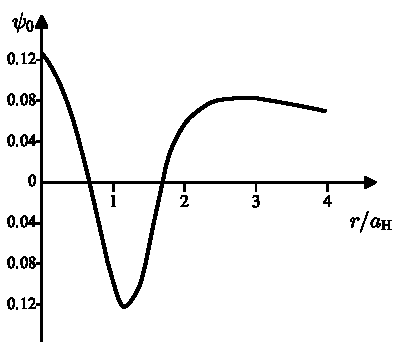
\includegraphics[width=6cm]{fig8-5.pdf}\\{\small 图 8.5\quad 金属Na导带底的维格纳-赛茨波函数}
\end{minipage}
\end{center}

金属的结合能由两部分组成：(i)自由原子的基态能 $E_{\mathrm{a}}$ 与导带底能量 $E_{0}$ 之差，(ii)导带中的电子平均动能等于 $\frac{3}{5}(\hbar^{2}k_{\mathrm{F}}^{2}/2m^{*})$，$m^{*}$ 为有效质量.金属Na的原子基态能 $E_{\mathrm{a}}$（即3s的电子能量）的实验测量值为 $-5.16$ eV，导带电子的平均动能
\begin{equation}
  \langle E_{\mathrm{F}}\rangle=\frac{3}{5}\frac{\hbar^{2}k_{\mathrm{F}}^{2}}{2m^{*}}
  =\frac{1.10}{r_{\mathrm{s}}^{2}}\frac{e^{2}}{a_{\mathrm{H}}}\Bigl(\frac{m}{m^{*}}\Bigr)
\end{equation}
若取 $m^{*}=m$，可算出 $\langle E_{\mathrm{F}}\rangle$ 约为 2.0 eV.由此求得的结合能为 $-1.1$ eV，与实验值 $-1.13$ eV 符合良好.

$E_{\mathrm{a}}$ 与 $E_{0}$ 的差别来源于边界条件的不同.对自由原子中电子边界条件应换为 $\left[\partial\psi_{0}(\boldsymbol{r})/\partial r\right]_{r=\infty}=0$，仍满足方程(8.5.12)，$V(r)$ 也取钠的离子实势.图8.6是Na的3s电子在自由原子状态（实线）和金属态（虚线）时波函数的示意图.显然，在固体中3s电子的分布更靠近离子实，因此有更低的势能，故 $|E_{0}|>|E_{\mathrm{a}}|$.

\begin{center}
\begin{minipage}{6cm}
\centering
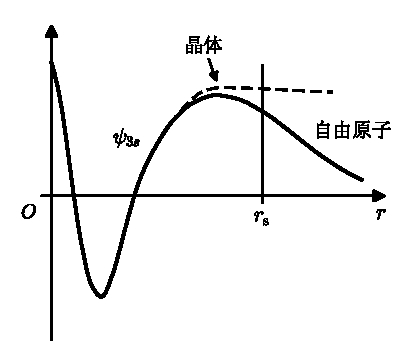
\includegraphics[width=6cm]{fig8-6.pdf}\\{\small 图 8.6\quad 维格纳-赛茨波函数和自由原子的3s波函数}
\end{minipage}
\end{center}
\subsection*{2. $\boldsymbol{k}=0$ 点附近有效质量的计算\textsuperscript{[11]}}

设价电子能带的底部在 $\boldsymbol{k}=0$ 处.为求得小 $k$ 状态的电子波函数和有效质量 $m^{*}$，应当从布洛赫函数
\begin{equation*}
  \psi_{\boldsymbol{k}}(\boldsymbol{r})=u_{\boldsymbol{k}}(\boldsymbol{r})\mathrm{e}^{\mathrm{i}\boldsymbol{k}\cdot\boldsymbol{r}}
\end{equation*}
出发，利用式(8.5.1)先写出 $u_{\boldsymbol{k}}(\boldsymbol{r})$ 所满足的方程
\begin{equation}
\begin{aligned}
  &-\frac{\hbar^{2}}{2m}(\nabla^{2}+2\mathrm{i}\boldsymbol{k}\cdot\nabla)u_{\boldsymbol{k}}(\boldsymbol{r})
  +V(\boldsymbol{r})u_{\boldsymbol{k}}(\boldsymbol{r})\\
  &\qquad=\Bigl(E-\frac{\hbar^{2}k^{2}}{2m}\Bigr)u_{\boldsymbol{k}}(\boldsymbol{r})
\end{aligned}
\end{equation}
其中 $u_{\boldsymbol{k}}(\boldsymbol{r})$ 是正点阵的周期函数.在W-S元胞内，$V(r)$ 为球形对称的离子实势.方程(8.5.14)与 $\psi_{0}(\boldsymbol{r})=u_{0}(r)$ 所满足的方程不同，其主要差别是出现了 $-\bigl(\mathrm{i}\hbar^{2}/m\bigr)\boldsymbol{k}\cdot\nabla u_{\boldsymbol{k}}$ 项，对于小 $k$ 值它可以当作微扰项处理.在讨论过程中仍可利用元胞法的球近似在 $0\leqslant r\leqslant r_{\mathrm{s}}$ 范围内作计算，并要求 $\psi_{0}$ 满足边界条件式(8.5.11).

将 $u_{\boldsymbol{k}}(\boldsymbol{r})$ 展开为 $k$ 的幂级数
\begin{equation}
\begin{aligned}
  u_{\boldsymbol{k}}(\boldsymbol{r})&=\sum_{n=0}^{\infty}u_{n}(\boldsymbol{r})k^{n}\\
  &=u_{0}(\boldsymbol{r})+u_{1}(\boldsymbol{r})k+\cdots\\
  &=\psi_{0}(\boldsymbol{r})+u_{1}(\boldsymbol{r})k+\cdots
\end{aligned}
\end{equation}
相似的，对于 $E_{k}$ 作展开，考虑到一级微扰能量正比于
\begin{equation}
  \int_{\Omega}\psi_{0}\boldsymbol{k}\cdot\nabla\psi_{0}\,\mathrm{d}\tau
  =\int_{\Omega}\psi_{0}\frac{\partial\psi_{0}}{\partial r}(\boldsymbol{k}\cdot\boldsymbol{r})\frac{1}{r}\,\mathrm{d}\tau=0
\end{equation}
是奇函数，故能量的一级修正等于零.准至 $k^{2}$ 项的 $E_{k}$ 展开式在球形近似下设为
\begin{equation}
  E_{k}=E_{0}+\alpha\,\frac{\hbar^{2}k^{2}}{2m}
\end{equation}
其中 $E_{0}$ 代表 $\boldsymbol{k}=0$ 的能量，$\alpha\equiv m/m^{*}$.将式(8.5.15)和(8.5.17)代入式(8.5.14)，求得 $\psi_{0}$ 与 $u_{1}$ 所满足的方程：
\begin{equation}
  \Bigl[-\nabla^{2}+\frac{2m}{\hbar^{2}}(V-E_{0})\Bigr]\psi_{0}=0
\end{equation}
\begin{equation}
  \Bigl[-\nabla^{2}+\frac{2m}{\hbar^{2}}(V-E_{0})\Bigr]u_{1}=2\mathrm{i}\,\boldsymbol{k}_{1}\cdot\nabla\psi_{0}
\end{equation}
其中 $\boldsymbol{k}_{1}$ 代表 $\boldsymbol{k}$ 方向单位矢
\begin{equation}
  \boldsymbol{k}_{1}\equiv\frac{\boldsymbol{k}}{k}
\end{equation}
设方程(8.5.18)的解 $\psi_{0}$ 和 $E_{0}$ 已经求得，现在主要任务是解方程(8.5.19).显然，$u_{1}(\boldsymbol{r})$ 是奇函数，又由于 $u_{1}(\boldsymbol{r})$ 应为正点阵的周期函数，因此经过W-S元胞多面体界面时，$u_{1}$ 将变号，这说明在边界面上 $u_{1}$ 必须等于零.若采用球近似可将 $u_{1}$ 的边界条件写为
\begin{equation}
  u_{1}(r)\Big|_{r=r_{\mathrm{s}}}=0
\end{equation}
式(8.5.19)的特解为
\begin{equation}
  -\mathrm{i}\,\boldsymbol{k}_{1}\cdot\boldsymbol{r}\,\psi_{0}(r)
\end{equation}
可直接代入方程(8.5.19)验证.为了满足边界条件式(8.5.21)，还必须加入式(8.5.19)的齐次方程解，可设其为
\begin{equation}
  \mathrm{i}(\boldsymbol{k}_{1}\cdot\boldsymbol{r}_{1})f_{\mathrm{p}}(r)\qquad
  \Bigl(\boldsymbol{r}_{1}\equiv\frac{\boldsymbol{r}}{r}\Bigr)
\end{equation}
将上式代入(8.5.19)，立刻得径向函数 $f_{\mathrm{p}}(r)$ 满足
\begin{equation}
  \frac{1}{r^{2}}\frac{\mathrm{d}}{\mathrm{d}r}\Bigl(r^{2}\frac{\mathrm{d}f_{\mathrm{p}}}{\mathrm{d}r}\Bigr)
  +\Bigl[\frac{2m}{\hbar^{2}}(E_{0}-V)-\frac{2}{r^{2}}\Bigr]f_{\mathrm{p}}=0
\end{equation}
与式(8.5.6)相比较可知，$f_{\mathrm{p}}$ 满足p波（$l=1$）的径向方程，式(8.5.23)也是反演操作的奇函数.因此，方程(8.5.19)的解为
\begin{equation}
  u_{1}(\boldsymbol{r})=\mathrm{i}(\boldsymbol{k}_{1}\cdot\boldsymbol{r})
  \Bigl[\frac{f_{\mathrm{p}}(r)}{r}-\psi_{0}(r)\Bigr]
\end{equation}
要求 $u_{1}(\boldsymbol{r})$ 满足边界条件式(8.5.21)，求得关系式
\begin{equation}
  f_{\mathrm{p}}(r_{\mathrm{s}})=r_{\mathrm{s}}\psi_{0}(r_{\mathrm{s}})
\end{equation}
利用求出的波函数代入式(8.5.15)，得
\begin{equation}
  \psi_{\boldsymbol{k}}(\boldsymbol{r})\approx\psi_{0}(\boldsymbol{r})+ku_{1}(\boldsymbol{r})
  =\psi_{0}+\mathrm{i}\,\boldsymbol{k}\cdot\boldsymbol{r}\,v(\boldsymbol{r})
\end{equation}
其中
\begin{equation}
  v(\boldsymbol{r})\equiv\frac{f_{\mathrm{p}}(r)}{r}-\psi_{0}(r)
\end{equation}
并设 $\psi_{\boldsymbol{k}}$ 满足归一条件
\begin{equation}
  \int_{\Omega}\psi_{\boldsymbol{k}}^{*}\psi_{\boldsymbol{k}}\,\mathrm{d}\tau=1
\end{equation}
则能带为
\begin{equation}
  E_{k}=\int_{\Omega}\psi_{\boldsymbol{k}}^{*}\Bigl[-\frac{\hbar^{2}}{2m}\nabla^{2}+V(\boldsymbol{r})\Bigr]\psi_{\boldsymbol{k}}\,\mathrm{d}\tau
\end{equation}
计算准至 $k^{2}$ 项的本征能量，可求得式(8.5.17)中的 $\alpha$ 为
\begin{equation}
  \alpha=1+\frac{2}{k^{2}}\int_{\Omega}\psi_{0}\Bigl[k^{2}v
  +\frac{1}{r}(\boldsymbol{k}\cdot\boldsymbol{r})^{2}\frac{\mathrm{d}v}{\mathrm{d}r}\Bigr]\mathrm{d}\tau
\end{equation}
这里 $\Omega$ 是W-S元胞，计算时近似取半径为 $r_{\mathrm{s}}$ 的球体.上式对角度积分后
\begin{equation}
  \alpha=1+8\pi\int_{0}^{r_{\mathrm{s}}}\psi_{0}(r)\Bigl[v(r)+\frac{r}{3}\Bigl(\frac{\mathrm{d}v}{\mathrm{d}r}\Bigr)\Bigr]r^{2}\,\mathrm{d}r
\end{equation}
再作部分积分，消去积分中第一项，得到
\begin{equation}
  \alpha=1-\frac{8\pi}{3}\int_{0}^{r_{\mathrm{s}}}v(r)\Bigl(\frac{\mathrm{d}\psi_{0}}{\mathrm{d}r}\Bigr)r^{3}\,\mathrm{d}r
\end{equation}
上式再经简化，可用 $r=r_{\mathrm{s}}$ 处的 $\psi_{0}$ 和 $v$ 表示 $\alpha$.为此，令
\begin{equation}
  \left.
  \begin{aligned}
    f_{\mathrm{p}}(r)&=\frac{P(r)}{r}\\
    \psi_{0}(r)&=\frac{R(r)}{r}
  \end{aligned}\right\}
\end{equation}
则
\begin{equation}
\begin{aligned}
  v(r)&=\frac{f_{\mathrm{p}}(r)}{r}-\psi_{0}(r)\\
  &=\frac{P(r)}{r^{2}}-\frac{R(r)}{r}
\end{aligned}
\end{equation}
相应的，将 $f_{\mathrm{p}}$ 与 $\psi_{0}$ 的方程(8.5.24)和(8.5.12)改写成
\begin{equation}
  \frac{\mathrm{d}^{2}R}{\mathrm{d}r^{2}}+\frac{2m}{\hbar^{2}}(E_{0}-V)R=0
\end{equation}
\begin{equation}
  \frac{\mathrm{d}^{2}P}{\mathrm{d}r^{2}}-\frac{2}{r^{2}}P+\frac{2m}{\hbar^{2}}(E_{0}-V)P=0
\end{equation}
用 $P(r)$ 和 $R(r)$ 表示的 $\alpha$ 为
\begin{equation}
  \alpha=1-\frac{8\pi}{3}\int_{0}^{r_{\mathrm{s}}}(P-rR)\Bigl(\frac{\mathrm{d}R}{\mathrm{d}r}-\frac{R}{r}\Bigr)\mathrm{d}r
\end{equation}
再利用下列关系式：

(i)由式(8.5.36)与(8.5.37)得
\begin{equation}
  R\Bigl(\frac{\mathrm{d}^{2}P}{\mathrm{d}r^{2}}\Bigr)-P\Bigl(\frac{\mathrm{d}^{2}R}{\mathrm{d}r^{2}}\Bigr)=\frac{2PR}{r^{2}}
\end{equation}

(ii)考虑 $\psi_{0}(\boldsymbol{r})=\dfrac{R(r)}{r}$ 在 $r_{\mathrm{s}}$ 球内近似归一
\begin{equation}
  \int_{\Omega}\psi_{0}^{2}\,\mathrm{d}\tau=\int_{0}^{r_{\mathrm{s}}}4\pi R^{2}(r)\,\mathrm{d}r\approx 1
\end{equation}
作分部积分可证明
\begin{equation}
  \frac{8\pi}{3}\int_{0}^{r_{\mathrm{s}}}rR\Bigl(\frac{\mathrm{d}R}{\mathrm{d}r}\Bigr)\mathrm{d}r
  =\frac{4\pi}{3}r_{\mathrm{s}}^{3}[\psi_{0}(r_{\mathrm{s}})]^{2}-\frac{1}{3}
\end{equation}

(iii)在 $r=r_{\mathrm{s}}$ 处 $\psi_{0}$ 满足 $\Bigl(\dfrac{\mathrm{d}\psi_{0}}{\mathrm{d}r}\Bigr)_{r_{\mathrm{s}}}=0$，$P(r_{\mathrm{s}})$ 的边界条件由式(8.5.26)和式(8.5.34)给出
\begin{equation}
  P(r_{\mathrm{s}})=r_{\mathrm{s}}R(r_{\mathrm{s}})
\end{equation}
可以证明
\begin{equation}
  \alpha=\gamma\Bigl[\Bigl(\frac{r}{P}\Bigr)\Bigl(\frac{\mathrm{d}P}{\mathrm{d}r}\Bigr)-1\Bigr]_{r=r_{\mathrm{s}}}
\end{equation}
其中
\begin{equation}
  \gamma\equiv\frac{4\pi}{3}r_{\mathrm{s}}^{3}[\psi_{0}(r_{\mathrm{s}})]^{2}
  =\frac{4\pi}{3}r_{\mathrm{s}}R^{2}(r_{\mathrm{s}})
\end{equation}
当 $\psi_{0}$ 已知时，只要从式(8.5.37)数值解出 $P(r)$，就能求得能带底部的有效质量 $m^{*}=m/\alpha$，从而得到 $\boldsymbol{k}=0$ 附近的电子能量.实际运算时，式(8.5.43)比式(8.5.33)更为方便.

元胞法的球近似尽管计算简单，但是所求得的结果仅与原子体积（或 $r_{\mathrm{s}}$）有关，它完全忽略了实际晶体结构的影响，假如计及晶体结构的影响，则必须使球函数的展开式在复杂的W-S元胞多面体界面上满足边界条件，对于BZ中的一般点，其数值计算工作量是相当大的，此外，从物理上看，在整个W-S元胞内都采用球对称的离子实势，也存在问题，因为W-S近似的势场在元胞边界处有导数的不连续性，如图8.7中实线所示.但是，实际上在这些地方势能的变化十分平滑，近似为常数势，如图8.7中虚线所示.鉴于以上困难，近年来元胞法已很少被采用，而代之以克服了上述缺点的新方法，例如格林函数方法和缀加平面波法.

\begin{center}
\begin{minipage}{6cm}
\centering
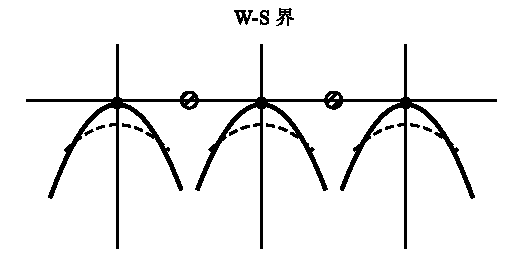
\includegraphics[width=6cm]{fig8-7.pdf}\\{\small 图 8.7\quad 元胞法势}
\end{minipage}
\end{center}
\section{缀加平面波法}

为了克服元胞法在W-S多面体上满足边界条件的困难，斯莱特（Slater）\textsuperscript{[12]}建议用丸盒势（muffin-tin potential）模型处理问题.所谓丸盒势即假定W-S元胞中球对称势仅限于离子实周围半径 $r_{\mathrm{i}}$ 的球体内，这些球彼此不相交如图8.8所示，称为M-T球.在M-T球外的元胞势场，则假定为常数势.适当选择能量的零点，可将W-S元胞内的丸盒势简单写成

\begin{center}
\begin{minipage}{5.5cm}
\centering
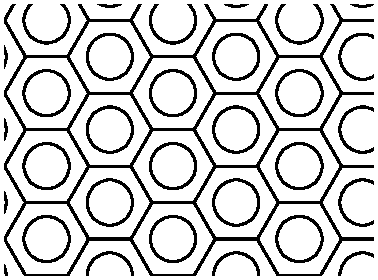
\includegraphics[width=5.5cm]{fig8-8.pdf}\\{\small 图 8.8\quad M-T球}
\end{minipage}
\end{center}

\begin{equation}
  V_{\mathrm{M\text{-}T}}(r)=\begin{cases}
    V(r) & (r<r_{\mathrm{i}})\\[0.2em]
    0 & (r\geqslant r_{\mathrm{i}})
  \end{cases}
\end{equation}
其中 $V(r)$ 是球对称的离子实势场，图8.9绘出了沿某离子线的丸盒势图.丸盒势模型将M-T球外的势场取为常数，显然更逼近实际情况，因为在这些地方薛定谔方程的解是平面波，而平面波在W-S多面体上能自动满足边界条件式(8.5.2)和(8.5.3).因此，丸盒势模型克服了元胞法满足边界条件的困难.在每个M-T球内，由于是球对称的势场，薛定谔方程的严格解可用径向波函数与球谐函数的乘积来展开表示

\begin{center}
\begin{minipage}{6cm}
\centering
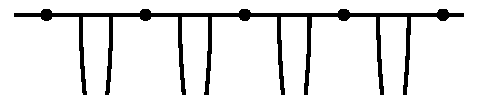
\includegraphics[width=6cm]{fig8-9.pdf}\\{\small 图 8.9\quad M-T势 $V_{\mathrm{M\text{-}T}}$}
\end{minipage}
\end{center}

\begin{equation}
  \phi_{\boldsymbol{k}}(\boldsymbol{r})=\begin{cases}
    \displaystyle\sum_{l,\,m}\mathrm{i}^{l}a_{lm}(\boldsymbol{k})\mathrm{Y}_{lm}(\theta,\phi)R_{l}(E_{k},r)
    & (r\leqslant r_{\mathrm{i}})\\[1.2em]
    \exp(\mathrm{i}\,\boldsymbol{k}\cdot\boldsymbol{r}) & (r>r_{\mathrm{i}})
  \end{cases}
\end{equation}
其中 $R_{l}(E_{k},r)$ 满足径向薛定谔方程
\begin{equation}
  \frac{1}{r^{2}}\frac{\mathrm{d}}{\mathrm{d}r}\Bigl(r^{2}\frac{\mathrm{d}R_{l}}{\mathrm{d}r}\Bigr)
  +\Bigl[\frac{2m}{\hbar^{2}}\bigl(E-V(r)\bigr)-\frac{l(l+1)}{r^{2}}\Bigr]R_{l}=0
\end{equation}
剩下的问题是如何使式(8.6.2)中的平面波与M-T球内球函数展开式相衔接.斯莱特要求 $\phi_{\boldsymbol{k}}(\boldsymbol{r})$ 在 $r=r_{\mathrm{i}}$ 处连续，从而决定系数 $a_{lm}$.将平面波用球谐函数展开：
\begin{equation}
  \mathrm{e}^{\mathrm{i}\boldsymbol{k}\cdot\boldsymbol{r}}=4\pi\sum_{l,\,m}\mathrm{i}^{l}\mathrm{j}_{l}(kr)\mathrm{Y}_{lm}(\theta,\phi)\mathrm{Y}_{lm}^{*}(\theta_{k},\phi_{k})
\end{equation}
其中 $(\theta,\phi)$ 是矢量 $\boldsymbol{r}$ 的方位角，$(\theta_{k},\phi_{k})$ 是 $\boldsymbol{k}$ 的方位角，$\mathrm{j}_{l}$ 为球贝塞尔函数，利用式(8.6.2)和 $r=r_{\mathrm{i}}$ 处 $\phi_{\boldsymbol{k}}$ 连续的条件，求得
\begin{equation}
  a_{lm}(\boldsymbol{k})=4\pi\mathrm{i}^{l}\bigl[\mathrm{j}_{l}(kr_{\mathrm{i}})/R_{l}(E_{k},r_{\mathrm{i}})\bigr]\mathrm{Y}_{lm}^{*}(\theta_{k},\phi_{k})
\end{equation}
将式(8.6.5)代入式(8.6.2)，所组成的 $\phi_{\boldsymbol{k}}(\boldsymbol{r})$ 称为缀加平面波（简称APW）.应当注意，APW与OPW不同之处在于平面波与球函数只在 $r=r_{\mathrm{i}}$ 处相接，而无重叠区.

晶体中单电子的布洛赫函数可由APW作基函数展开表示：
\begin{equation}
  \psi_{\boldsymbol{k}}(\boldsymbol{r})=\sum_{\boldsymbol{K}}\alpha(\boldsymbol{k}+\boldsymbol{K})\phi_{\boldsymbol{k}+\boldsymbol{K}}(\boldsymbol{r})
\end{equation}

\begin{center}
\begin{minipage}{6cm}
\centering
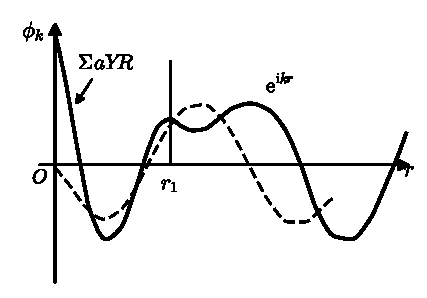
\includegraphics[width=6cm]{fig8-10.pdf}\\{\small 图 8.10\quad APW示意图}
\end{minipage}
\end{center}

其中 $\alpha(\boldsymbol{k}+\boldsymbol{K})$ 为待定系数，$\boldsymbol{K}$ 为倒格矢，而APW可根据式(8.6.2)与(8.6.5)写成
\begin{equation}
\begin{aligned}
  \phi_{\boldsymbol{k}+\boldsymbol{K}}(\boldsymbol{r})
  &=\mathrm{e}^{\mathrm{i}(\boldsymbol{k}+\boldsymbol{K})\cdot\boldsymbol{r}}\eta(\boldsymbol{r}-\boldsymbol{r}_{\mathrm{i}})
  +\eta(\boldsymbol{r}_{\mathrm{i}}-\boldsymbol{r})\sum_{l,\,m}4\pi\mathrm{i}^{l}\mathrm{j}_{l}(|\boldsymbol{k}+\boldsymbol{K}|\,r_{\mathrm{i}})\cdot\\
  &\qquad\Bigl[\frac{R_{l}(E_{k},\boldsymbol{r})}{R_{l}(E_{k},r_{\mathrm{i}})}\Bigr]\mathrm{Y}_{lm}(\theta,\phi)\mathrm{Y}_{lm}^{*}(\theta_{k},\phi_{k})
\end{aligned}
\end{equation}
这里 $\eta(x)$ 是阶跃函数：
\begin{equation}
  \eta(x)=\begin{cases}
    1 & (x>0)\\
    0 & (x<0)
  \end{cases}
\end{equation}
由于 $\phi_{\boldsymbol{k}+\boldsymbol{K}}(\boldsymbol{r})$ 在 $r=r_{\mathrm{i}}$ 处具有导数不连续性，应当利用附录G中的变分原理来确定 $E_{k}$ 和系数 $\alpha(\boldsymbol{k}+\boldsymbol{K})$.具体做法如下：

（i）以 $\psi_{\boldsymbol{k}}=\sum_{\boldsymbol{K}}\alpha(\boldsymbol{k}+\boldsymbol{K})\phi_{\boldsymbol{k}+\boldsymbol{K}}$ 作为试探变分函数，代入能量泛函公式［见式(G.3)］
\begin{equation}
  \int_{\Omega}\Bigl\{\frac{\hbar^{2}}{2m}|\nabla\psi_{\boldsymbol{k}}|^{2}+V|\psi_{\boldsymbol{k}}|^{2}\Bigr\}\mathrm{d}\tau
  -E[\psi_{\boldsymbol{k}}]\int_{\Omega}\psi_{\boldsymbol{k}}^{*}\psi_{\boldsymbol{k}}\,\mathrm{d}\tau=0
\end{equation}

（ii）作变分时应要求泛函 $E[\psi_{\boldsymbol{k}}]$ 对于 $\psi_{\boldsymbol{k}}$ 是稳定的，这时 $E$ 才是晶体中单电子薛定谔方程的能带解.当 $\alpha^{*}$ 变化时，这一要求简单表示为
\begin{equation}
  \frac{\partial E[\psi_{\boldsymbol{k}}]}{\partial\alpha^{*}}=0
\end{equation}

（iii）式(8.6.9)对 $\alpha^{*}$ 变分，并利用式(8.6.10)，可求得 $\alpha(\boldsymbol{k}+\boldsymbol{K})$ 的线性齐次方程组
\begin{equation}
  \sum_{\boldsymbol{K}'}\langle\boldsymbol{k}+\boldsymbol{K}|M|\boldsymbol{k}+\boldsymbol{K}'\rangle_{\mathrm{APW}}\alpha(\boldsymbol{k}+\boldsymbol{K}')=0
\end{equation}
其中
\begin{equation}
\begin{aligned}
  &\langle\boldsymbol{k}+\boldsymbol{K}|M|\boldsymbol{k}+\boldsymbol{K}'\rangle_{\mathrm{APW}}\\
  &\quad=\int_{\Omega}\mathrm{d}\tau\Bigl\{\frac{\hbar^{2}}{2m}\nabla\phi_{\boldsymbol{k}+\boldsymbol{K}}^{*}\cdot\nabla\phi_{\boldsymbol{k}+\boldsymbol{K}'}
  +(V-E)\phi_{\boldsymbol{k}+\boldsymbol{K}}^{*}\phi_{\boldsymbol{k}+\boldsymbol{K}'}\Bigr\}
\end{aligned}
\end{equation}
这里 $\boldsymbol{K}$、$\boldsymbol{K}'$ 均为倒格矢.

（iv）能量本征值 $E_{k}$ 由式(8.6.11)的系数行列式等于零决定：
\begin{equation}
  \mathrm{det}\,\|\langle\boldsymbol{k}+\boldsymbol{K}|M|\boldsymbol{k}+\boldsymbol{K}'\rangle_{\mathrm{APW}}\|=0
\end{equation}
具体计算 $M$ 的APW矩阵元时，应将元胞 $\Omega$ 分为M-T球内部分 $\Omega_{\mathrm{I}}=\dfrac{4\pi}{3}r_{\mathrm{i}}^{3}$ 和球外部分 $\Omega_{\mathrm{II}}$：
\begin{equation}
  \Omega=\Omega_{\mathrm{I}}+\Omega_{\mathrm{II}}
\end{equation}
由于 $r_{\mathrm{i}}$ 球外部分 $V(\boldsymbol{r})=0$，$\phi_{\boldsymbol{k}+\boldsymbol{K}}$ 为平面波 $\mathrm{e}^{\mathrm{i}(\boldsymbol{k}+\boldsymbol{K})\cdot\boldsymbol{r}}$，其计算十分方便.将式(8.6.1)和(8.6.2)代入式(8.6.12)，可将球外APW对 $M$ 矩阵元的贡献写成
\begin{equation}
\begin{aligned}
  &\Bigl(\int_{\Omega}-\int_{\Omega_{\mathrm{I}}}\Bigr)\mathrm{d}\tau
  \Bigl\{\frac{\hbar^{2}}{2m}\nabla\mathrm{e}^{-\mathrm{i}(\boldsymbol{k}+\boldsymbol{K})\cdot\boldsymbol{r}}\cdot\nabla\mathrm{e}^{\mathrm{i}(\boldsymbol{k}+\boldsymbol{K}')\cdot\boldsymbol{r}}
  -E\,\mathrm{e}^{\mathrm{i}(\boldsymbol{K}'-\boldsymbol{K})\cdot\boldsymbol{r}}\Bigr\}\\
  &\quad=\Bigl[\frac{\hbar^{2}}{2m}(\boldsymbol{k}+\boldsymbol{K})\cdot(\boldsymbol{k}+\boldsymbol{K}')-E\Bigr]
  \Bigl\{\int_{\Omega}\mathrm{e}^{\mathrm{i}(\boldsymbol{K}'-\boldsymbol{K})\cdot\boldsymbol{r}}\mathrm{d}\tau\\
  &\qquad-\int_{\Omega_{\mathrm{I}}}\mathrm{e}^{\mathrm{i}(\boldsymbol{K}'-\boldsymbol{K})\cdot\boldsymbol{r}}\mathrm{d}\tau\Bigr\}
\end{aligned}
\end{equation}
利用关系式
\begin{equation}
  \int_{\Omega}\mathrm{e}^{\mathrm{i}(\boldsymbol{K}'-\boldsymbol{K})\cdot\boldsymbol{r}}\mathrm{d}\tau=\Omega\,\delta_{\boldsymbol{K}\boldsymbol{K}'}
\end{equation}
和
\begin{equation}
  \int_{\Omega_{\mathrm{I}}}\mathrm{e}^{\mathrm{i}\boldsymbol{p}\cdot\boldsymbol{r}}\mathrm{d}\tau
  =4\pi\int_{0}^{r_{\mathrm{i}}}\Bigl(\frac{\sin pr}{pr}\Bigr)r^{2}\,\mathrm{d}r
  =4\pi r_{\mathrm{i}}^{2}\frac{\mathrm{j}_{1}(pr_{\mathrm{i}})}{p}
\end{equation}
最后求得平面波部分对 $M$ 的贡献为
\begin{equation}
  \Bigl\{\frac{\hbar^{2}}{2m}(\boldsymbol{k}+\boldsymbol{K})\cdot(\boldsymbol{k}+\boldsymbol{K}')-E\Bigr\}
  \Bigl\{\Omega\delta_{\boldsymbol{K}\boldsymbol{K}'}
  -4\pi r_{\mathrm{i}}^{2}\frac{\mathrm{j}_{1}(|\boldsymbol{K}'-\boldsymbol{K}|\,r_{\mathrm{i}})}{|\boldsymbol{K}'-\boldsymbol{K}|}\Bigr\}
\end{equation}
球内部分 $M$ 矩阵元的计算比较复杂，这里只说明步骤.对式(8.6.12)右边第一项作部分积分，并利用格林定理，得到关系式
\begin{equation}
\begin{aligned}
  \int_{\Omega_{\mathrm{I}}}\nabla\phi_{\boldsymbol{k}+\boldsymbol{K}}^{*}\cdot\nabla\phi_{\boldsymbol{k}+\boldsymbol{K}'}\,\mathrm{d}\tau&\\
  =\int_{\Omega_{\mathrm{I}}}\phi_{\boldsymbol{k}+\boldsymbol{K}}^{*}(-\nabla^{2})\phi_{\boldsymbol{k}+\boldsymbol{K}'}\,\mathrm{d}\tau
  +\int_{S}\phi_{\boldsymbol{k}+\boldsymbol{K}}^{*}\nabla\phi_{\boldsymbol{k}+\boldsymbol{K}'}\cdot\mathrm{d}\boldsymbol{S}&
\end{aligned}
\end{equation}
其中 $S$ 代表 $r_{\mathrm{i}}$ 球面，则 $\langle\boldsymbol{k}+\boldsymbol{K}|M|\boldsymbol{k}+\boldsymbol{K}'\rangle_{\mathrm{APW}}$ 的球内部分贡献可表示为
\begin{equation}
  \int_{\Omega_{\mathrm{I}}}\nabla\phi_{\boldsymbol{k}+\boldsymbol{K}}^{*}\Bigl[-\frac{\hbar^{2}}{2m}\nabla^{2}+V(r)-E\Bigr]\phi_{\boldsymbol{k}+\boldsymbol{K}'}\,\mathrm{d}\tau
  +\int_{S}\phi_{\boldsymbol{k}+\boldsymbol{K}}^{*}\frac{\partial}{\partial\eta}\phi_{\boldsymbol{k}+\boldsymbol{K}'}\,\mathrm{d}S
\end{equation}
面积分中的 $\eta$ 是M-T球面的外法线.式(8.6.20)中的体积分等于零.因为在 $r<r_{\mathrm{i}}$ 时 $(H-E)\phi_{\boldsymbol{k}+\boldsymbol{K}'}=0$ 与径向方程(8.6.3)一致，这说明APW在M-T球内满足薛定谔方程.面积分部分要利用球函数的正交条件及其辅助定理，斯莱特计算的最后结果为
\begin{equation}
\begin{aligned}
  4\pi r_{\mathrm{i}}^{2}\sum_{l=0}^{\infty}(2l+1)\mathrm{P}_{l}(\cos\theta_{\boldsymbol{K}\boldsymbol{K}'})\mathrm{j}_{l}(|\boldsymbol{k}+\boldsymbol{K}|\,r_{\mathrm{i}})\times\\
  \mathrm{j}_{l}(|\boldsymbol{k}+\boldsymbol{K}'|\,r_{\mathrm{i}})\frac{R_{l}'(E,r_{\mathrm{i}})}{R_{l}(E,r_{\mathrm{i}})}
\end{aligned}
\end{equation}
其中 $R_{l}'\equiv\dfrac{\mathrm{d}R_{l}}{\mathrm{d}r}$，$\theta_{\boldsymbol{K}\boldsymbol{K}'}$ 为 $\boldsymbol{K}$ 与 $\boldsymbol{K}'$ 间夹角，具体推导可参考原文\textsuperscript{[19]}.式(8.6.21)与式(8.6.18)之和即是 $\langle\boldsymbol{k}+\boldsymbol{K}|M|\boldsymbol{k}+\boldsymbol{K}'\rangle_{\mathrm{APW}}$，可整理成对角及非对角部分之和
\begin{equation}
  \frac{1}{\Omega}\langle\boldsymbol{k}+\boldsymbol{K}|M|\boldsymbol{k}+\boldsymbol{K}'\rangle_{\mathrm{APW}}
  =\Bigl[\frac{\hbar^{2}}{2m}(\boldsymbol{k}+\boldsymbol{K})^{2}-E\Bigr]\delta_{\boldsymbol{K}\boldsymbol{K}'}
  +\Gamma_{\boldsymbol{K}\boldsymbol{K}'}
\end{equation}
这里非对角矩阵元 $\Gamma_{\boldsymbol{K}\boldsymbol{K}'}$ 定义为
\begin{equation}
\begin{aligned}
  \Gamma_{\boldsymbol{K}\boldsymbol{K}'}&\equiv\frac{4\pi r_{\mathrm{i}}^{2}}{\Omega}\biggl\{
  -\Bigl[\frac{\hbar^{2}}{2m}(\boldsymbol{k}+\boldsymbol{K})\cdot(\boldsymbol{k}+\boldsymbol{K}')-E\Bigr]
  \frac{\mathrm{j}_{1}(|\boldsymbol{K}'-\boldsymbol{K}|\,r_{\mathrm{i}})}{|\boldsymbol{K}'-\boldsymbol{K}|}\\
  &\quad+\sum_{l=0}^{\infty}(2l+1)\mathrm{P}_{l}(\cos\theta_{\boldsymbol{K}\boldsymbol{K}'})\mathrm{j}_{l}(|\boldsymbol{k}+\boldsymbol{K}|\,r_{\mathrm{i}})\cdot\\
  &\qquad\mathrm{j}_{l}(|\boldsymbol{k}+\boldsymbol{K}'|\,r_{\mathrm{i}})\frac{R_{l}'(E,r_{\mathrm{i}})}{R_{l}(E,r_{\mathrm{i}})}\biggr\}
\end{aligned}
\end{equation}
根据式(8.6.22)的记号，可将方程(8.6.11)写成与平面波法中式(8.1.11)相似的形式
\begin{equation}
  \Bigl\{\frac{\hbar^{2}(\boldsymbol{k}+\boldsymbol{K})^{2}}{2m}-E\Bigr\}_{\boldsymbol{K}}\alpha(\boldsymbol{k}+\boldsymbol{K})
  +\sum_{\boldsymbol{K}'(\boldsymbol{K}'\neq\boldsymbol{K})}\Gamma_{\boldsymbol{K}\boldsymbol{K}'}\alpha(\boldsymbol{k}+\boldsymbol{K}')=0
\end{equation}
类似的，久期方程(8.6.13)变为与(8.1.13)相似的表示式
\begin{equation}
  \mathrm{det}\,\Bigl\|\Bigl[\frac{\hbar^{2}}{2m}(\boldsymbol{k}+\boldsymbol{K})^{2}-E\Bigr]\delta_{\boldsymbol{K}\boldsymbol{K}'}
  +\Gamma_{\boldsymbol{K}\boldsymbol{K}'}\Bigr\|=0
\end{equation}
显然，$\Gamma_{\boldsymbol{K}\boldsymbol{K}'}$ 相当于有效势的傅里叶分量，由于APW法将M-T球外的平面波与M-T球内的原子波函数在 $r=r_{\mathrm{i}}$ 处连续相接，同样也将在离子实区引进振荡，与OPW有相似之处.因此，式(8.6.23)中的 $\Gamma_{\boldsymbol{K}\boldsymbol{K}'}$ 与OPW法中的 $\langle\boldsymbol{k}+\boldsymbol{K}|U|\boldsymbol{k}+\boldsymbol{K}'\rangle$［见式(8.2.14)］应有相似的抵消特性，就是说用APW法展开来表示 $\psi_{\boldsymbol{k}}$ 也具有比平面波方法收敛更快的优点.

应当指出，由于APW波函数是彼此不正交的，久期行列式(8.6.25)中对角与非对角元都明显含 $E$，此外能量 $E$ 还在 $\Gamma_{\boldsymbol{K}\boldsymbol{K}'}$ 表示式的 $R_{l}'(E,r_{\mathrm{i}})/R_{l}(E,r_{\mathrm{i}})$ 函数中出现.因此，利用APW法作能带计算时，首先要在能量 $E$ 时解出径向薛定谔方程(8.6.3)，并算出M-T球面上 $R_{l}$ 的对数导数值
\begin{equation*}
  \frac{\mathrm{d}}{\mathrm{d}r}\bigl\{\ln R_{l}(E,r)\bigr\}_{r=r_{\mathrm{i}}}=R_{l}'(E,r_{\mathrm{i}})/R_{l}(E,r_{\mathrm{i}})
\end{equation*}
然后，对于给定的波矢 $\boldsymbol{k}$ 按式(8.6.23)计算不同倒格矢之间的矩阵元，调整 $E$，直到久期行列式等于零时，才能定出能带电子的能量本征值 $E_{k}$.显然，这一计算过程的工作量相当大.但是，在电子计算机高度发展的今日已非难事，特别是在式(8.6.23)中出现的都是一些标准函数，它们都有现成的子程序可利用.此外，还可以利用晶体对称性降低久期行列式的维数，使计算简化.APW法既具有元胞法便于利用对称性的优点，又克服了元胞法在W-S元胞面上满足边界条件的困难.实践证明，APW法用于金属能带的计算是相当成功的，所算出的能带结构和费密面与实验符合良好\textsuperscript{[14]}，包括含d带的贵金属（Cu、Ag、Au）和过渡金属，而对于这些金属OPW法却不能应用.

APW法不适用于共价键半导体，这是与丸盒势模型密切有关的.对于呈密排结构的单价金属，可以认为在离子周围势场是球对称的，而在离子之间势场变化缓慢，因此M-T势适用于这些金属.但是，对于共价键晶体，如Ge、Si等属于四面体键，其原子势场的方向性变化很大，原子周围的势场既不是球对称的，而且在原子之间势场也不是缓慢变化的，与丸盒势模型差异较大，因此，APW法不能应用.
\section{KKR方法}

这是柯林嘎（Korringa）\textsuperscript{[15]}、孔恩（Kohn）和罗斯托克尔（Rostoker）\textsuperscript{[16]}所提出的另一种计算能带的有效方法，通常称为格林函数方法，或简称KKR法.KKR法与前面所介绍的能带计算法不同，它不是根据物理情况选择展开基函数，而是先把单电子运动方程化为积分方程，再用散射方法求解能态.其主要内容如下：

为了求解能带电子的薛定谔方程
\begin{equation}
  \Bigl(\frac{\hbar^{2}}{2m}\nabla^{2}+E\Bigr)\psi_{\boldsymbol{k}}(\boldsymbol{r})=V(\boldsymbol{r})\psi_{\boldsymbol{k}}(\boldsymbol{r})
\end{equation}
引入下列点源势方程
\begin{equation}
  \Bigl(\frac{\hbar^{2}}{2m}\nabla^{2}+E\Bigr)G(\boldsymbol{r},\boldsymbol{r}')=\delta(\boldsymbol{r}-\boldsymbol{r}')
\end{equation}
其中 $G(\boldsymbol{r},\boldsymbol{r}')$ 是单电子薛定谔方程的格林函数，式(8.7.2)又称为格林函数方程.利用 $G(\boldsymbol{r},\boldsymbol{r}')$ 可将微分方程(8.7.1)改写为积分方程
\begin{equation}
  \psi_{\boldsymbol{k}}(\boldsymbol{r})=\int_{\Omega}G(\boldsymbol{r},\boldsymbol{r}')V(\boldsymbol{r}')\psi_{\boldsymbol{k}}(\boldsymbol{r}')\,\mathrm{d}^{3}r'
\end{equation}
若用算子 $\Bigl(\dfrac{\hbar^{2}}{2m}\nabla^{2}+E\Bigr)$ 作用于式(8.7.3)的两边，再利用 $G(\boldsymbol{r},\boldsymbol{r}')$ 的方程(8.7.2)，可以立刻导出式(8.7.1)：
\begin{equation*}
\begin{aligned}
  \Bigl(\frac{\hbar^{2}}{2m}\nabla^{2}+E\Bigr)\psi_{\boldsymbol{k}}(\boldsymbol{r})
  &=\int_{\Omega}\Bigl[\Bigl(\frac{\hbar^{2}}{2m}\nabla^{2}+E\Bigr)G(\boldsymbol{r},\boldsymbol{r}')\Bigr]V(\boldsymbol{r}')\psi_{\boldsymbol{k}}(\boldsymbol{r}')\,\mathrm{d}^{3}r'\\
  &=\int_{\Omega}\delta(\boldsymbol{r}-\boldsymbol{r}')V(\boldsymbol{r}')\psi_{\boldsymbol{k}}(\boldsymbol{r}')\,\mathrm{d}^{3}r'\\
  &=V(\boldsymbol{r})\psi_{\boldsymbol{k}}(\boldsymbol{r})
\end{aligned}
\end{equation*}
说明式(8.7.3)与式(8.7.1)是等效的表示式.KKR方法的特点是利用式(8.7.3)，由格林函数 $G(\boldsymbol{r},\boldsymbol{r}')$ 求 $\psi_{\boldsymbol{k}}(\boldsymbol{r})$ 和 $E_{n}(\boldsymbol{k})$.

为了使所求得 $\psi_{\boldsymbol{k}}(\boldsymbol{r})$ 满足布洛赫定理，KKR要求晶体的 $G(\boldsymbol{r},\boldsymbol{r}')$ 也满足布洛赫定理
\begin{equation}
  G(\boldsymbol{r}+\boldsymbol{l},\boldsymbol{r}')=\mathrm{e}^{\mathrm{i}\boldsymbol{k}\cdot\boldsymbol{l}}G(\boldsymbol{r},\boldsymbol{r}')
\end{equation}
这是格林函数所满足的边界条件.根据量子力学\textsuperscript{[17]}，$G(\boldsymbol{r},\boldsymbol{r}')$ 由公式
\begin{equation}
  G(\boldsymbol{r},\boldsymbol{r}')=\sum_{j}\phi_{j}^{*}(\boldsymbol{r}')(E-E_{j})^{-1}\phi_{j}(\boldsymbol{r})
\end{equation}
决定，其中 $\phi_{j}$ 与 $E_{j}$ 代表式(8.7.2)的齐次方程的本征函数和本征值，满足方程
\begin{equation}
  \Bigl(\frac{\hbar^{2}}{2m}\nabla^{2}+E_{j}\Bigr)\phi_{j}(\boldsymbol{r})=0
\end{equation}
和完备性条件
\begin{equation}
  \sum_{j}\phi_{j}^{*}(\boldsymbol{r}')\phi_{j}(\boldsymbol{r})=\delta(\boldsymbol{r}-\boldsymbol{r}')
\end{equation}
不难验证，$G(\boldsymbol{r},\boldsymbol{r}')$ 的解式(8.7.5)满足格林函数方程(8.7.2)，因为从式(8.7.5)出发，利用式(8.7.6)和式(8.7.7)，能立刻求出式(8.7.2)：
\begin{equation*}
  \Bigl(\frac{\hbar^{2}}{2m}\nabla^{2}+E\Bigr)G(\boldsymbol{r},\boldsymbol{r}')
  =\sum_{j}\frac{\phi_{j}^{*}(\boldsymbol{r}')\Bigl(\dfrac{\hbar^{2}}{2m}\nabla^{2}+E\Bigr)\phi_{j}(\boldsymbol{r})}{E-E_{j}}
  =\sum_{j}\phi_{j}^{*}(\boldsymbol{r}')\phi_{j}(\boldsymbol{r})=\delta(\boldsymbol{r}-\boldsymbol{r}')
\end{equation*}
应注意，式(8.7.6)实际上是自由电子的定态薛定谔方程，因此满足布洛赫定理的 $\phi_{j}(\boldsymbol{r})$ 应取为
\begin{equation}
  \phi_{j}(\boldsymbol{r})=\Omega^{-1/2}\exp\bigl[\mathrm{i}(\boldsymbol{k}+\boldsymbol{K})\cdot\boldsymbol{r}\bigr]
\end{equation}
代表在元胞 $\Omega$ 内归一的一平面波，$\boldsymbol{k}\in\mathrm{BZ}$，而 $\boldsymbol{K}$ 为倒格矢.将上式代入式(8.7.5)，求得满足式(8.7.4)的格林函数.
\begin{equation}
  G(\boldsymbol{r},\boldsymbol{r}')=\frac{1}{\Omega}\sum_{\boldsymbol{K}}
  \frac{\exp\bigl[\mathrm{i}(\boldsymbol{k}+\boldsymbol{K})\cdot(\boldsymbol{r}-\boldsymbol{r}')\bigr]}
  {E-\dfrac{\hbar^{2}}{2m}(\boldsymbol{k}+\boldsymbol{K})^{2}}
\end{equation}
应当看到，对于确定的 $E$ 和 $\boldsymbol{k}$，这个 $\boldsymbol{K}$ 的求和式只因晶体结构而异.因此，$G(\boldsymbol{r},\boldsymbol{r}')$ 又称为结构格林函数.KKR法的主要步骤为，首先严格计算结构格林函数的求和式(8.7.9)，再由 $G$ 近似定 $E_{n}(\boldsymbol{k})$ 和 $\psi_{\boldsymbol{k}}(\boldsymbol{r})$.

作具体计算时，与缀加平面波法相同，也采用M-T势作近似.这时，由于在M-T球外 $V(\boldsymbol{r})=0\ (r>r_{\mathrm{i}})$，因此确定 $\psi_{\boldsymbol{k}}(\boldsymbol{r})$ 的方程只需在M-T球内积分
\begin{equation}
  \psi_{\boldsymbol{k}}(\boldsymbol{r})=\int_{r'\leqslant r_{\mathrm{i}}-\varepsilon}
  G(\boldsymbol{r},\boldsymbol{r}')V(\boldsymbol{r}')\psi_{\boldsymbol{k}}(\boldsymbol{r}')\,\mathrm{d}^{3}r'
  \qquad(\varepsilon=0^{+})
\end{equation}
再考虑到 $r<r_{\mathrm{i}}$ 时，$V(r)=V(r)$，代表球对称的离子实势，我们可以假定M-T球内能带电子波函数由球谐函数展开表示
\begin{equation}
  \psi_{\boldsymbol{k}}(\boldsymbol{r})=\sum_{l,\,m}C_{lm}R_{l}(r)\mathrm{Y}_{lm}(\theta,\phi)
\end{equation}
其中系数 $C_{lm}$ 待定.为导出 $C_{lm}$ 的方程，相应的将M-T球内 $G(\boldsymbol{r},\boldsymbol{r}')$ 也用球谐函数表示\textsuperscript{[18]}
\begin{equation}
\begin{aligned}
  G(\boldsymbol{r},\boldsymbol{r}')
  =\sum_{lm}\sum_{l'm'}&\bigl\{\mathrm{i}^{l-l'}A_{lm,\,l'm'}\mathrm{j}_{l}(gr)\mathrm{j}_{l'}(gr')\\
  &+g\,\delta_{ll'}\delta_{mm'}\mathrm{j}_{l}(gr)\mathrm{n}_{l'}(gr')\bigr\}\times\\
  &\mathrm{Y}_{lm}(\theta,\phi)\mathrm{Y}_{l'm'}^{*}(\theta',\phi')\qquad(r<r'<r_{\mathrm{i}})
\end{aligned}
\end{equation}
其中 $\mathrm{n}_{l}$ 是 $l$ 阶诺伊曼（Neumann）函数，当取里德伯原子单位时\footnote{当取 $1\,[\mathrm{Ry}]=(\hbar^{2}/2ma_{\mathrm{H}}^{2})=(e^{2}/2a_{\mathrm{H}})$ 作为能量的单位时，相当于取 $\hbar=2m=1$，$e^{2}=2$ 和 $a_{\mathrm{H}}$ 为长度的单位.}，$g$ 代表能量因子
\begin{equation}
  g=\sqrt{E}\ \ (E>0);\qquad g=\mathrm{i}\sqrt{(-E)}\ \ (E<0)
\end{equation}
而常数 $A_{lm,\,l'm'}$ 可按标准方法计算\textsuperscript{[19]}，它们只与晶体结构有关，因此 $A_{lm,\,l'm'}$ 称为结构常数.属于同类型点阵的不同晶体，$A_{lm,\,l'm'}$ 的计算只需进行一次，这是KKR方法在计算上的优点之一.

利用式(8.7.1)和式(8.7.2)，消去式(8.7.10)中的M-T势，再由积分的格林定理容易求出下列面积分等式：
\begin{equation}
  \int_{r_{\mathrm{i}}-\varepsilon}\bigl\{G(\boldsymbol{r},\boldsymbol{r}')\nabla'\psi_{\boldsymbol{k}}(\boldsymbol{r}')
  -\psi_{\boldsymbol{k}}(\boldsymbol{r}')\nabla'G(\boldsymbol{r},\boldsymbol{r}')\bigr\}\cdot\mathrm{d}\boldsymbol{S}'=0
\end{equation}
积分在 $r_{\mathrm{i}}-\varepsilon$ 球面上进行.再将 $\psi_{\boldsymbol{k}}$ 和 $G$ 的球函数表示式(8.7.11)和式(8.7.12)代入上式，利用 $\mathrm{Y}_{lm}$ 的正交性，最后取 $\varepsilon\to 0$，可求得 $C_{lm}$ 的久期方程式，而 $C_{lm}$ 有非零解的条件是久期方程的系数行列式等于零.
\begin{equation}
  \mathrm{det}\,\biggl\|A_{lm,\,l'm'}
  +g\,\delta_{ll'}\delta_{mm'}\frac{(\mathrm{n}_{l}L_{l}-\mathrm{n}_{l}')}{(\mathrm{j}_{l}L_{l}-\mathrm{j}_{l}')}\biggr\|=0
\end{equation}
由此可计算能带 $E_{n}(\boldsymbol{k})$.其中
\begin{equation*}
  \mathrm{j}_{l}'=\Bigl[\frac{\mathrm{d}\,\mathrm{j}_{l}(gr)}{\mathrm{d}(gr)}\Bigr]_{r=r_{\mathrm{i}}},\qquad
  \mathrm{n}_{l}'=\Bigl[\frac{\mathrm{d}\,\mathrm{n}_{l}(gr)}{\mathrm{d}(gr)}\Bigr]_{r=r_{\mathrm{i}}}
\end{equation*}
分别是 $r=r_{\mathrm{i}}$ 处贝塞尔与诺伊曼函数的导数，而 $L_{l}$ 是M-T球面上的径向函数的对数导数
\begin{equation}
  L_{l}=\frac{\mathrm{d}}{\mathrm{d}r}\bigl[\ln R_{l}(r)\bigr]_{r=r_{\mathrm{i}}}
  =\frac{R_{l}'(r_{\mathrm{i}})}{R_{l}(r_{\mathrm{i}})}
\end{equation}
由于 $R_{l}(r)$ 满足径向方程(8.6.3)，所以久期行列式(8.7.15)中第二项是和M-T球内离子实势有关的，它与晶体结构无关，而第一项 $A_{lm,\,l'm'}$ 则仅与晶体结构有关，它和M-T势无关.因此，在KKR的行列式中，反映晶体结构几种特征的项和代表原子特征的项是彼此独立的.KKR法的这一特点，将使能带计算的效率提高.

比较APW和KKR的久期行列式(8.6.25)和式(8.7.15)可以看出，APW是按倒格矢 $\boldsymbol{K}$ 排列的行列式，而KKR行列式则按球谐函数的 $lm$ 排列.严格讲，两者都是无穷阶的行列式.当作近似计算时，APW对 $\boldsymbol{K}$ 切断，而KKR法则对 $l$ 作切断.实际利用式(8.7.15)作能带计算时，往往只需计算少数低 $l$ 项的贡献，因为当慢电子被一个球形原子势散射时，高 $l$ 的分波效应是可以忽略的.KKR法不仅成功用于金属能带计算\textsuperscript{[20]}，并已推广为处理无序系的一个有效方法\textsuperscript{[21]}.

值得注意的是，KKR久期行列式的非对角矩阵元和APW一样，也是能量 $E$ 的函数.因此，在KKR法中，也不能利用矩阵对角化办法求给定 $\boldsymbol{k}$ 的所有 $E$ 值，而必须在确定 $\boldsymbol{k}$ 时，输入各种 $E$ 值计算矩阵元，并经多次循环，最后找到满足式(8.7.15)的 $E$ 值，它才是电子能量的许可值.近年来提出了Muffin-tin轨道线性组合（LMTO）方法\textsuperscript{[22]}，它是KKR法的“线性化”形式，保留了KKR法的优点，但经线性化后单电子哈密顿量的矩阵元已与能量 $E$ 无关，从而避免了KKR法的上述困难.类似的，在APW法基础上也发展了线性化缀加平面波（LAPW）法\textsuperscript{[23]}.这些线性化方法已成为处理元胞内含多个原子的晶体和过渡金属的表面等复杂系统的普遍方法.
\section{布洛赫表象和瓦尼尔表象}

到此为止，我们仅讨论了理想晶体的能带理论，并充分利用了晶格周期性.当存在外场或杂质和缺陷时，除周期场中单电子哈密顿量 $H$ 以外，还应计入外加势场 $U$，涉及下列薛定谔方程的求解问题：
\begin{equation}
  \left.
  \begin{aligned}
    &\mathrm{i}\hbar\frac{\partial\Psi}{\partial t}=(H+U)\Psi\\
    &H=-\frac{\hbar^{2}}{2m}\nabla^{2}+V(\boldsymbol{r}),\qquad V(\boldsymbol{r}+\boldsymbol{l})=V(\boldsymbol{r})
  \end{aligned}\right\}
\end{equation}
在处理上述问题时，可以用理想晶体的 $H$ 所决定的完整函数组作为基函数，展开表示波函数 $\Psi$.以布洛赫函数作基函数表示的 $\Psi$ 称布洛赫表象.此外，我们还可以通过布洛赫函数定义另一套描述局域状态的完整函数组——瓦尼尔函数，由它表示的 $\Psi$ 构成瓦尼尔表象.下面分别介绍这两种表象，为简单起见将假定能带是非简并的.

\subsection*{1. 布洛赫表象}

由于布洛赫函数 $\psi_{n\boldsymbol{k}}(\boldsymbol{r})$ 是理想晶体中单电子哈密顿量 $H$ 的本征函数
\begin{equation}
  H\psi_{n\boldsymbol{k}}(\boldsymbol{r})=E_{n}(\boldsymbol{k})\psi_{n\boldsymbol{k}}(\boldsymbol{r})
\end{equation}
这里 $n$ 是能带指标，$\boldsymbol{k}$ 为波矢，$(n,\boldsymbol{k})$ 是描述完整晶体单电子状态的量子数.根据量子力学，厄密算符 $H$ 的不同本征值状态之间应彼此正交，适当选择归一化因子，可使布洛赫函数 $\psi_{n\boldsymbol{k}}(\boldsymbol{r})$ 满足下列正交归一条件：
\begin{equation}
  \int_{N\Omega}\psi_{n\boldsymbol{k}}^{*}(\boldsymbol{r})\psi_{n'\boldsymbol{k}'}(\boldsymbol{r})\,\mathrm{d}\boldsymbol{r}
  =\delta_{nn'}\delta_{\boldsymbol{k}\boldsymbol{k}'}
\end{equation}
除了上述正交性条件以外，布洛赫函数的完备性条件可按下述讨论给出：

若用不同 $n$，$\boldsymbol{k}$ 的 $\psi_{n\boldsymbol{k}}(\boldsymbol{r})$ 构成完整函数组，则任意波函数 $\Psi$ 可由它们展开表示
\begin{equation}
  \Psi(\boldsymbol{r})=\sum_{n,\,\boldsymbol{k}}C_{n\boldsymbol{k}}\psi_{n\boldsymbol{k}}(\boldsymbol{r})
\end{equation}
其中
\begin{equation}
  C_{n\boldsymbol{k}}=\int\Psi(\boldsymbol{r})\psi_{n\boldsymbol{k}}^{*}(\boldsymbol{r})\,\mathrm{d}\boldsymbol{r}
\end{equation}
将式(8.8.5)代入式(8.8.4)，求得
\begin{equation}
  \Psi(\boldsymbol{r})=\int\Psi(\boldsymbol{r}')\Bigl\{\sum_{n,\,\boldsymbol{k}}\psi_{n\boldsymbol{k}}^{*}(\boldsymbol{r}')\psi_{n\boldsymbol{k}}(\boldsymbol{r})\Bigr\}\mathrm{d}\boldsymbol{r}'
\end{equation}
由式(8.8.6)可知 $\Psi$ 展开式成立的条件为
\begin{equation}
  \sum_{n,\,\boldsymbol{k}}\psi_{n\boldsymbol{k}}^{*}(\boldsymbol{r}')\psi_{n\boldsymbol{k}}(\boldsymbol{r})=\delta(\boldsymbol{r}-\boldsymbol{r}')
\end{equation}
这就是布洛赫函数的完备性条件.

\subsection*{2. 瓦尼尔表象}

由于布洛赫函数 $\psi_{n\boldsymbol{k}}(\boldsymbol{r})$ 是倒点阵的周期函数
\begin{equation}
  \psi_{n\boldsymbol{k}}(\boldsymbol{r})=\psi_{n,\,\boldsymbol{k}+\boldsymbol{K}}(\boldsymbol{r})
\end{equation}
根据第一章§5，$\psi_{n\boldsymbol{k}}$ 可按正格矢展开为傅里叶级数
\begin{equation}
  \psi_{n\boldsymbol{k}}(\boldsymbol{r})=N^{-1/2}\sum_{\boldsymbol{l}}\mathrm{e}^{\mathrm{i}\boldsymbol{k}\cdot\boldsymbol{l}}a_{n}(\boldsymbol{r},\boldsymbol{l})
\end{equation}
利用
\begin{equation*}
  N^{-1}\sum_{\boldsymbol{k}\in\mathrm{BZ}}\mathrm{e}^{\mathrm{i}\boldsymbol{k}\cdot(\boldsymbol{l}-\boldsymbol{l}')}=\delta_{\boldsymbol{l}\boldsymbol{l}'}
\end{equation*}
求得其逆变换为
\begin{equation}
  a_{n}(\boldsymbol{r},\boldsymbol{l})=N^{-1/2}\sum_{\boldsymbol{k}\in\mathrm{BZ}}\mathrm{e}^{-\mathrm{i}\boldsymbol{k}\cdot\boldsymbol{l}}\psi_{n\boldsymbol{k}}(\boldsymbol{r})
\end{equation}
函数 $a_{n}(\boldsymbol{r},\boldsymbol{l})$ 与波矢 $\boldsymbol{k}$ 无关，只是位置的函数.利用布洛赫定理
\begin{equation}
  \psi_{n\boldsymbol{k}}(\boldsymbol{r}-\boldsymbol{l})=\mathrm{e}^{-\mathrm{i}\boldsymbol{k}\cdot\boldsymbol{l}}\psi_{n\boldsymbol{k}}(\boldsymbol{r})
\end{equation}
可将(8.8.10)改写为
\begin{equation}
  a_{n}(\boldsymbol{r},\boldsymbol{l})=N^{-1/2}\sum_{\boldsymbol{k}\in\mathrm{BZ}}\psi_{n\boldsymbol{k}}(\boldsymbol{r}-\boldsymbol{l})
  =a_{n}(\boldsymbol{r}-\boldsymbol{l})
\end{equation}
上式说明 $a_{n}(\boldsymbol{r},\boldsymbol{l})$ 只是矢量差 $(\boldsymbol{r}-\boldsymbol{l})$ 的函数.式(8.8.10)所定义的函数 $a_{n}(\boldsymbol{r}-\boldsymbol{l})$ 称为瓦尼尔函数.不同的能带 $n$，不同的格点 $\boldsymbol{l}$ 有不同的瓦尼尔函数.利用布洛赫函数的正交性和完备性，不难证明瓦尼尔函数 $a_{n}(\boldsymbol{r}-\boldsymbol{l})$ 也构成完整正交函数组.

(i)瓦尼尔函数的正交性
\begin{equation}
\begin{aligned}
  &\int a_{n}^{*}(\boldsymbol{r}-\boldsymbol{l})a_{n'}(\boldsymbol{r}-\boldsymbol{l}')\,\mathrm{d}\boldsymbol{r}\\
  &\quad=N^{-1}\sum_{\boldsymbol{k}}\sum_{\boldsymbol{k}'}
  \mathrm{e}^{\mathrm{i}\boldsymbol{k}\cdot\boldsymbol{l}-\mathrm{i}\boldsymbol{k}'\cdot\boldsymbol{l}'}
  \int\psi_{n\boldsymbol{k}}^{*}(\boldsymbol{r})\psi_{n'\boldsymbol{k}'}(\boldsymbol{r})\,\mathrm{d}\boldsymbol{r}\\
  &\quad=\frac{1}{N}\sum_{\boldsymbol{k}\in\mathrm{BZ}}\mathrm{e}^{\mathrm{i}\boldsymbol{k}\cdot(\boldsymbol{l}-\boldsymbol{l}')}\delta_{nn'}
  =\delta_{nn'}\delta_{\boldsymbol{l}\boldsymbol{l}'}
\end{aligned}
\end{equation}
不同格点 $\boldsymbol{l}$ 的瓦尼尔函数彼此正交，进一步说明了 $a_{n}(\boldsymbol{r}-\boldsymbol{l})$ 具有定域特性.作为瓦尼尔函数的一个例子，我们设式(8.8.10)中布洛赫函数为
\begin{equation}
  \psi_{n\boldsymbol{k}}(\boldsymbol{r})=N^{-1/2}u_{n}(\boldsymbol{r})\mathrm{e}^{\mathrm{i}\boldsymbol{k}\cdot\boldsymbol{r}}
\end{equation}
其中周期函数 $u_{n}(\boldsymbol{r})$ 近似与 $\boldsymbol{k}$ 无关，则由式(8.8.12)
\begin{equation}
  a_{n}(\boldsymbol{r}-\boldsymbol{l})=\frac{1}{N}\sum_{\boldsymbol{k}\in\mathrm{BZ}}u_{n}(\boldsymbol{r}-\boldsymbol{l})\mathrm{e}^{\mathrm{i}\boldsymbol{k}\cdot(\boldsymbol{r}-\boldsymbol{l})}
\end{equation}
对于立方胞边长为 $a$ 的简立方晶格，瓦尼尔函数为
\begin{equation}
  a_{n}(\boldsymbol{r}-\boldsymbol{l})=u_{n}(\boldsymbol{r}-\boldsymbol{l})
  \frac{\sin\bigl(\dfrac{\pi X}{a}\bigr)\sin\bigl(\dfrac{\pi Y}{a}\bigr)\sin\bigl(\dfrac{\pi Z}{a}\bigr)}
  {\bigl(\pi X/a\bigr)\bigl(\pi Y/a\bigr)\bigl(\pi Z/a\bigr)}
\end{equation}
其中 $\boldsymbol{r}-\boldsymbol{l}\equiv X\boldsymbol{i}+Y\boldsymbol{j}+Z\boldsymbol{k}$.显然，$a_{n}(\boldsymbol{r}-\boldsymbol{l})$ 是以 $\boldsymbol{l}$ 为中心的振荡衰减函数.

(ii)瓦尼尔函数的完备性
\begin{equation}
\begin{aligned}
  \sum_{n}\sum_{\boldsymbol{l}}a_{n}^{*}(\boldsymbol{r}-\boldsymbol{l})a_{n}(\boldsymbol{r}'-\boldsymbol{l})&\\
  =\frac{1}{N}\sum_{\boldsymbol{k}}\sum_{\boldsymbol{k}'}\sum_{\boldsymbol{l}}
  \mathrm{e}^{\mathrm{i}\boldsymbol{k}\cdot\boldsymbol{l}-\mathrm{i}\boldsymbol{k}'\cdot\boldsymbol{l}}
  \sum_{n}\psi_{n\boldsymbol{k}}^{*}(\boldsymbol{r})\psi_{n'\boldsymbol{k}'}(\boldsymbol{r}')&\\
  =\sum_{\boldsymbol{k}}\sum_{\boldsymbol{k}'}\delta_{\boldsymbol{k}\boldsymbol{'}}
  \Bigl[\sum_{n}\psi_{n\boldsymbol{k}}^{*}(\boldsymbol{r})\psi_{n'\boldsymbol{k}'}(\boldsymbol{r}')\Bigr]&\\
  =\sum_{n}\sum_{\boldsymbol{k}}\psi_{n\boldsymbol{k}}^{*}(\boldsymbol{r})\psi_{n\boldsymbol{k}}(\boldsymbol{r}')&\\
  =\delta(\boldsymbol{r}-\boldsymbol{r}')&
\end{aligned}
\end{equation}
这里利用了布洛赫函数的完备性条件.因此，也可以用瓦尼尔函数作基函数表示波函数 $\Psi(\boldsymbol{r})$，构成瓦尼尔表象.

\subsection*{3. 布洛赫与瓦尼尔表象中的二次量子化算符}

既然布洛赫函数和瓦尼尔函数都是完备函数组，我们可以用这两套函数作基底表示希尔伯特（Hilbert）空间的态矢量，在布洛赫表象中的态矢量为
\begin{equation}
  \Psi(\boldsymbol{r})=\sum_{n,\,\boldsymbol{k}}C_{n\boldsymbol{k}}\psi_{n\boldsymbol{k}}(\boldsymbol{r})
\end{equation}
而在瓦尼尔表象为
\begin{equation}
  \Psi(\boldsymbol{r})=\sum_{n,\,\boldsymbol{l}}C_{n\boldsymbol{l}}a_{n}(\boldsymbol{r}-\boldsymbol{l})
\end{equation}
其中 $C_{n\boldsymbol{k}}$ 是布洛赫表象中电子的消灭算符，$C_{n\boldsymbol{l}}$ 为瓦尼尔表象中的消灭算符，代表在 $n$ 能带 $\boldsymbol{l}$ 格点局域态上消灭一个电子，因此式(8.8.19)又称为态矢量的局域表示.

两种表象中的算符变换关系可利用式(8.8.19)，式(8.8.11)和式(8.8.12)代入式(8.8.18)导出
\begin{equation*}
  \sum_{n,\,\boldsymbol{k}}C_{n\boldsymbol{k}}\psi_{n\boldsymbol{k}}(\boldsymbol{r})
  =\sum_{n,\,\boldsymbol{l}}C_{n\boldsymbol{l}}a_{n}(\boldsymbol{r}-\boldsymbol{l})
  =\sum_{n,\,\boldsymbol{k}}\Bigl\{\frac{1}{\sqrt{N}}\sum_{\boldsymbol{l}}C_{n\boldsymbol{l}}\mathrm{e}^{-\mathrm{i}\boldsymbol{k}\cdot\boldsymbol{l}}\Bigr\}\psi_{n\boldsymbol{k}}(\boldsymbol{r})
\end{equation*}
由此求得
\begin{equation}
  C_{n\boldsymbol{k}}=\frac{1}{\sqrt{N}}\sum_{\boldsymbol{l}}C_{n\boldsymbol{l}}\mathrm{e}^{-\mathrm{i}\boldsymbol{k}\cdot\boldsymbol{l}}
\end{equation}
其逆变换为
\begin{equation}
  C_{n\boldsymbol{l}}=\frac{1}{\sqrt{N}}\sum_{\boldsymbol{k}\in\mathrm{BZ}}C_{n\boldsymbol{k}}\mathrm{e}^{\mathrm{i}\boldsymbol{k}\cdot\boldsymbol{l}}
\end{equation}
式(8.8.20)和(8.8.21)是两种表象的算符变换关系，而式(8.8.9)和(8.8.10)则代表两种基底间的变换关系.

当讨论单带问题时，往往略去带指标 $n$，但计入自旋指标 $\sigma$，从而将式(8.8.20)和式(8.8.21)写成
\begin{equation}
  \left.
  \begin{aligned}
    &C_{\boldsymbol{k}\sigma}=\frac{1}{\sqrt{N}}\sum_{\boldsymbol{l}}C_{\boldsymbol{l}\sigma}\mathrm{e}^{-\mathrm{i}\boldsymbol{k}\cdot\boldsymbol{l}};
    \qquad
    C_{\boldsymbol{k}\sigma}^{+}=\frac{1}{\sqrt{N}}\sum_{\boldsymbol{l}}C_{\boldsymbol{l}\sigma}^{+}\mathrm{e}^{\mathrm{i}\boldsymbol{k}\cdot\boldsymbol{l}}\\
    &C_{\boldsymbol{l}\sigma}=\frac{1}{\sqrt{N}}\sum_{\boldsymbol{k}\in\mathrm{BZ}}C_{\boldsymbol{k}\sigma}\mathrm{e}^{\mathrm{i}\boldsymbol{k}\cdot\boldsymbol{l}};
    \qquad
    C_{\boldsymbol{l}\sigma}^{+}=\frac{1}{\sqrt{N}}\sum_{\boldsymbol{k}\in\mathrm{BZ}}C_{\boldsymbol{k}\sigma}^{+}\mathrm{e}^{-\mathrm{i}\boldsymbol{k}\cdot\boldsymbol{l}}
  \end{aligned}\right\}
\end{equation}
其中 $C_{\boldsymbol{k}\sigma}^{+}$ 和 $C_{\boldsymbol{l}\sigma}^{+}$ 分别为布洛赫及瓦尼尔表象中电子的产生算符，这些算符都满足费密子的对易关系.式(8.8.22)是固体理论中的常用公式，但应注意，变换关系只适用于完整晶格，因为在推导时利用了平移对称性.

\subsection*{4. 瓦尼尔函数方程}

布洛赫函数是完整晶体中单电子哈密顿量 $H$ 的本征函数，它满足式(8.8.2).在同一能带 $n$ 中，不同波矢 $\boldsymbol{k}$，对应于不同的能量本征值 $E_{n}(\boldsymbol{k})$.根据式(8.8.10)，瓦尼尔函数 $a_{n}(\boldsymbol{r}-\boldsymbol{l})$ 是由不同波矢 $\boldsymbol{k}$［即不同能量 $E_{n}(\boldsymbol{k})$］的布洛赫函数组合构成的，它当然不是 $H$ 的本征函数.瓦尼尔函数的 $H$ 矩阵元为
\begin{equation}
\begin{aligned}
  &\int a_{n}^{*}(\boldsymbol{r}-\boldsymbol{l})Ha_{n'}(\boldsymbol{r}-\boldsymbol{l}')\,\mathrm{d}\boldsymbol{r}\\
  &\quad=\frac{1}{N}\sum_{\boldsymbol{k}}\sum_{\boldsymbol{k}'}
  \mathrm{e}^{\mathrm{i}\boldsymbol{k}\cdot\boldsymbol{l}-\mathrm{i}\boldsymbol{k}'\cdot\boldsymbol{l}'}
  \int\psi_{n\boldsymbol{k}}^{*}H\psi_{n'\boldsymbol{k}'}\,\mathrm{d}\boldsymbol{r}\\
  &\quad=\delta_{nn'}\frac{1}{N}\sum_{\boldsymbol{k}\in\mathrm{BZ}}\mathrm{e}^{\mathrm{i}\boldsymbol{k}\cdot(\boldsymbol{l}-\boldsymbol{l}')}E_{n}(\boldsymbol{k})
\end{aligned}
\end{equation}
利用能带函数是倒点阵的周期函数
\begin{equation}
  E_{n}(\boldsymbol{k}+\boldsymbol{K})=E_{n}(\boldsymbol{k})
\end{equation}
将 $E_{n}(\boldsymbol{k})$ 按正格矢展开为
\begin{equation}
  E_{n}(\boldsymbol{k})=\sum_{\boldsymbol{l}}\mathrm{e}^{\mathrm{i}\boldsymbol{k}\cdot\boldsymbol{l}}\mathscr{E}_{n}(\boldsymbol{l})
\end{equation}
其傅里叶系数为
\begin{equation}
  \mathscr{E}_{n}(\boldsymbol{l})=\frac{1}{N}\sum_{\boldsymbol{k}\in\mathrm{BZ}}\mathrm{e}^{-\mathrm{i}\boldsymbol{k}\cdot\boldsymbol{l}}E_{n}(\boldsymbol{k})
\end{equation}
而 $H$ 的矩阵元写成
\begin{equation}
  \int a_{n}^{*}(\boldsymbol{r}-\boldsymbol{l})Ha_{n'}(\boldsymbol{r}-\boldsymbol{l}')\,\mathrm{d}\boldsymbol{r}
  =\delta_{nn'}\mathscr{E}_{n}(\boldsymbol{l}'-\boldsymbol{l})
\end{equation}
其中存在着非对角元素，它们是不同格点瓦尼尔函数的 $H$ 矩阵元.

根据布洛赫函数的定态薛定谔方程(8.8.2)，容易导出瓦尼尔函数所满足的方程.将式(8.8.9)代入式(8.8.2)得
\begin{equation}
  \sum_{\boldsymbol{l}'}\mathrm{e}^{\mathrm{i}\boldsymbol{k}\cdot\boldsymbol{l}'}Ha_{n}(\boldsymbol{r}-\boldsymbol{l}')
  =\sum_{\boldsymbol{l}'}\mathrm{e}^{\mathrm{i}\boldsymbol{k}\cdot\boldsymbol{l}'}E_{n}(\boldsymbol{k})a_{n}(\boldsymbol{r}-\boldsymbol{l}')
\end{equation}
乘 $N^{-1}\mathrm{e}^{-\mathrm{i}\boldsymbol{k}\cdot\boldsymbol{l}}$，并在BZ中对 $\boldsymbol{k}$ 求和
\begin{equation}
  \sum_{\boldsymbol{l}'}\Bigl\{\frac{1}{N}\sum_{\boldsymbol{k}\in\mathrm{BZ}}\mathrm{e}^{-\mathrm{i}\boldsymbol{k}\cdot(\boldsymbol{l}-\boldsymbol{l}')}\Bigr\}Ha_{n}(\boldsymbol{r}-\boldsymbol{l}')
  =\sum_{\boldsymbol{l}'}\Bigl\{\frac{1}{N}\sum_{\boldsymbol{k}\in\mathrm{BZ}}\mathrm{e}^{-\mathrm{i}\boldsymbol{k}\cdot(\boldsymbol{l}-\boldsymbol{l}')}E_{n}(\boldsymbol{k})\Bigr\}a_{n}(\boldsymbol{r}-\boldsymbol{l}')
\end{equation}
再利用式(8.8.26)，最后求得瓦尼尔函数方程
\begin{equation}
  Ha_{n}(\boldsymbol{r}-\boldsymbol{l})
  =\sum_{\boldsymbol{l}'}\mathscr{E}_{n}(\boldsymbol{l}-\boldsymbol{l}')a_{n}(\boldsymbol{r}-\boldsymbol{l}')
\end{equation}
显然，$a_{n}(\boldsymbol{r}-\boldsymbol{l})$ 不是 $H$ 的本征函数，这说明用瓦尼尔函数计算完整晶体的能带是不方便的.但是，用瓦尼尔表象讨论局域杂质的电子能谱却十分有效.特别当局域杂质势 $U(\boldsymbol{r})$ 较强时，薛定谔方程的微扰法失效，这时利用瓦尼尔函数展开表示式(8.8.1)中的 $\Psi(\boldsymbol{r},t)$ 可以得出一个有效哈密顿量，其求解十分方便.
\section{有效哈密顿量}

现在讨论式(8.8.1)具有能量本征值 $E$ 的解
\begin{equation}
\begin{gathered}
  \mathrm{i}\hbar\frac{\partial\Psi}{\partial t}=E\Psi\\[0.2em]
  \bigl[H+U(\boldsymbol{r})\bigr]\Psi(\boldsymbol{r})=E\Psi(\boldsymbol{r})
\end{gathered}
\end{equation}
在瓦尼尔表象中以 $a_{n}(\boldsymbol{r}-\boldsymbol{l})$ 作基函数展开表示 $\Psi$
\begin{equation}
  \Psi(\boldsymbol{r})=\sum_{n,\,\boldsymbol{l}}F_{n}(\boldsymbol{l})a_{n}(\boldsymbol{r}-\boldsymbol{l})
\end{equation}
将式(8.9.2)代入(8.9.1)，乘以 $a_{n}^{*}(\boldsymbol{r}-\boldsymbol{l})$ 并对 $\boldsymbol{r}$ 作积分，则利用瓦尼尔函数的正交归一性和式(8.8.27)，求得
\begin{equation}
\begin{aligned}
  \sum_{\boldsymbol{l}'}\bigl[\mathscr{E}_{n}(\boldsymbol{l}'-\boldsymbol{l})-E\delta_{\boldsymbol{l},\,\boldsymbol{l}'}\bigr]F_{n}(\boldsymbol{l}')\\
  +\sum_{n',\,\boldsymbol{l}'}U_{nn'}(\boldsymbol{l},\boldsymbol{l}')F_{n'}(\boldsymbol{l}')=0
\end{aligned}
\end{equation}
其中
\begin{equation}
  U_{nn'}(\boldsymbol{l},\boldsymbol{l}')
  =\int a_{n}^{*}(\boldsymbol{r}-\boldsymbol{l})U(\boldsymbol{r})a_{n'}(\boldsymbol{r}-\boldsymbol{l}')\,\mathrm{d}\boldsymbol{r}
\end{equation}
式(8.9.3)可看作为瓦尼尔表象中的薛定谔方程.如果只有少数矩阵元 $U_{nn'}(\boldsymbol{l},\boldsymbol{l}')$ 不为零，则式(8.9.3)可以直接求解.一般情况下求解很复杂，涉及大量的原子集团计算.

一种有效的解法是，假设已知完整晶体的能带结构函数 $E_{n}(\boldsymbol{k})$ 的，并将 $E_{n}(\boldsymbol{k})$ 的宗量用 $-\mathrm{i}\nabla$ 代替，从而构造一个算子 $E_{n}(-\mathrm{i}\nabla)$，将它作用于连续函数 $F_{n}(\boldsymbol{r})$，从式(8.8.25)可得到下列重要关系式：
\begin{equation}
\begin{aligned}
  E_{n}(-\mathrm{i}\nabla)F_{n}(\boldsymbol{r})
  &=\sum_{\boldsymbol{l}}\mathscr{E}_{n}(\boldsymbol{l})\mathrm{e}^{\boldsymbol{l}\cdot\nabla}F_{n}(\boldsymbol{r})\\
  &=\sum_{\boldsymbol{l}}\mathscr{E}_{n}(\boldsymbol{l})\Bigl[1+\boldsymbol{l}\cdot\nabla+\frac{1}{2}(\boldsymbol{l}\cdot\nabla)^{2}+\cdots\Bigr]F_{n}(\boldsymbol{r})\\
  &=\sum_{\boldsymbol{l}}\mathscr{E}_{n}(\boldsymbol{l})\Bigl[F_{n}(\boldsymbol{r})+\boldsymbol{l}\cdot\nabla F_{n}(\boldsymbol{r})\\
  &\qquad+\frac{1}{2}\sum_{i,\,j=1}^{3}l_{i}l_{j}\frac{\partial}{\partial x_{i}}\frac{\partial}{\partial x_{j}}F_{n}(\boldsymbol{r})+\cdots\Bigr]\\
  &=\sum_{\boldsymbol{l}}\mathscr{E}_{n}(\boldsymbol{l})F_{n}(\boldsymbol{r}+\boldsymbol{l})
\end{aligned}
\end{equation}
称为瓦尼尔关系，将式(8.9.3)的第一项写成
\begin{equation}
\begin{aligned}
  \sum_{\boldsymbol{l}'}\mathscr{E}_{n}(\boldsymbol{l}'-\boldsymbol{l})F_{n}(\boldsymbol{l}')
  &=\sum_{\boldsymbol{l}'}\mathscr{E}_{n}(\boldsymbol{l}')F_{n}(\boldsymbol{l}+\boldsymbol{l}')\\
  &=\Bigl[\sum_{\boldsymbol{l}'}\mathscr{E}_{n}(\boldsymbol{l}')F_{n}(\boldsymbol{r}+\boldsymbol{l}')\Bigr]_{\boldsymbol{r}=\boldsymbol{l}}\\
  &=\bigl[E_{n}(-\mathrm{i}\nabla)F_{n}(\boldsymbol{r})\bigr]_{\boldsymbol{r}=\boldsymbol{l}}
\end{aligned}
\end{equation}
最后一个等式利用了瓦尼尔关系.因此，式(8.9.3)可表示为下列差分方程：
\begin{equation}
  \bigl[E_{n}(-\mathrm{i}\nabla)F_{n}(\boldsymbol{r})-EF_{n}(\boldsymbol{r})\bigr]_{\boldsymbol{r}=\boldsymbol{l}}
  +\sum_{n',\,\boldsymbol{l}'}U_{nn'}(\boldsymbol{l},\boldsymbol{l}')F_{n'}(\boldsymbol{l}')=0
\end{equation}
而连续函数 $F_{n}(\boldsymbol{r})$ 满足微分方程
\begin{equation}
  E_{n}(-\mathrm{i}\nabla)F_{n}(\boldsymbol{r})
  +\sum_{n',\,\boldsymbol{l}'}U_{nn'}(\boldsymbol{r},\boldsymbol{l}')F_{n'}(\boldsymbol{l}')=EF_{n}(\boldsymbol{r})
\end{equation}
注意式(8.9.8)中单电子在周期势场中的哈密顿量 $H$ 已被有效哈密顿量 $E_{n}(-\mathrm{i}\nabla)$ 所代替.式(8.9.8)是严格的.若不作近似，其复杂程度与式(8.9.3)一样.

对于非简并能带情况，往往可以略去带间跃迁，即在式(8.9.7)中令 $U_{nn'}(\boldsymbol{l},\boldsymbol{l}')$ 的 $n'\neq n$ 矩阵元为零，从而简化为单带问题.再假定势场 $U(\boldsymbol{r})$ 在晶格距离上缓慢变化，式(8.9.4)中的 $U(\boldsymbol{r})$ 可从积分号内抽出，这时利用瓦尼尔函数正交归一性得到
\begin{equation}
  U_{nn'}(\boldsymbol{l},\boldsymbol{l}')\approx[U(r)]_{r=l}\,\delta_{nn'}\delta_{\boldsymbol{l}\boldsymbol{l}'}
\end{equation}
于是连续函数 $F_{n}(\boldsymbol{r})$ 的方程(8.9.8)可近似写为
\begin{equation}
  E_{n}(-\mathrm{i}\nabla)F_{n}(\boldsymbol{r})+U(\boldsymbol{r})F_{n}(\boldsymbol{r})=EF_{n}(\boldsymbol{r})
\end{equation}
对于含时问题，相应的方程为
\begin{equation}
  \bigl[E_{n}(-\mathrm{i}\nabla)+U(\boldsymbol{r})\bigr]F_{n}(\boldsymbol{r},t)
  =\mathrm{i}\hbar\frac{\partial}{\partial t}F_{n}(\boldsymbol{r},t)
\end{equation}
式(8.9.10)，(8.9.11)和出发的方程(8.9.1)相比较是更为简单的，因为在这里单电子的周期势场 $V(\boldsymbol{r})$ 不再出现，我们可以直接应用能带论解出的 $E_{n}(\boldsymbol{k})$，构造有效哈密顿量.例如半导体材料（如Ge和Si等）在能带极值点附近，等能面为旋转椭球
\begin{equation}
  E_{n}(\boldsymbol{k})=E_{n}(\boldsymbol{k}_{0})
  +\frac{\hbar^{2}}{2m_{\mathrm{T}}}k_{t}^{2}
  +\frac{\hbar^{2}}{2m_{\mathrm{L}}}k_{l}^{2}
\end{equation}
其中 $m_{\mathrm{T}}$、$m_{\mathrm{L}}$ 分别为横向及纵向有效质量.若取 $E_{n}(\boldsymbol{k}_{0})$ 为能量 $E$ 的原点，并设转轴沿 $z$ 方向，则有效哈密顿量可简单写成
\begin{equation*}
  -\frac{\hbar^{2}}{2m_{\mathrm{T}}}\Bigl(\frac{\partial^{2}}{\partial x^{2}}+\frac{\partial^{2}}{\partial y^{2}}\Bigr)
  -\frac{\hbar^{2}}{2m_{\mathrm{L}}}\frac{\partial^{2}}{\partial z^{2}}
\end{equation*}
这时方程(8.9.10)变为
\begin{equation}
  \Bigl[-\frac{\hbar^{2}}{2m_{\mathrm{T}}}\Bigl(\frac{\partial^{2}}{\partial x^{2}}+\frac{\partial^{2}}{\partial y^{2}}\Bigr)
  -\frac{\hbar^{2}}{2m_{\mathrm{L}}}\frac{\partial^{2}}{\partial z^{2}}+U(\boldsymbol{r})\Bigr]F(\boldsymbol{r})=EF(\boldsymbol{r})
\end{equation}
称为有效质量方程.当半导体中杂质含量很少时，$U(\boldsymbol{r})$ 可取下列单杂质势
\begin{equation}
  U(\boldsymbol{r})=-\frac{e^{2}}{\varepsilon r}
\end{equation}
其中 $\varepsilon$ 代表半导体的介电常数.这时 $F(\boldsymbol{r})$ 的方程(8.9.13)与氢原子问题中的薛定谔方程相似，差别仅在于 $F$ 方程中用了介电常数和各向异性的有效质量.对于球形等能面
\begin{equation}
  m_{\mathrm{T}}=m_{\mathrm{L}}=m^{*}
\end{equation}
方程(8.9.13)简化为类氢原子问题
\begin{equation}
  \Bigl[-\frac{\hbar^{2}}{2m^{*}}\nabla^{2}-\frac{e^{2}}{\varepsilon r}\Bigr]F(\boldsymbol{r})=EF(\boldsymbol{r})
\end{equation}
这时形成以杂质为中心的电子局域态，可以直接搬用氢原子的结构求得基态能量和波函数为
\begin{equation}
  \left.
  \begin{aligned}
    &E_{1}=-\frac{m^{*}e^{4}}{2\varepsilon^{2}\hbar^{2}}
    =\frac{1}{\varepsilon^{2}}\frac{m^{*}}{m}E_{\mathrm{H}}\\[0.3em]
    &F(\boldsymbol{r})=\frac{1}{\sqrt{\pi}}\Bigl(\frac{1}{a_{\mathrm{H}}^{*}}\Bigr)^{3/2}\exp(-r/a_{\mathrm{H}}^{*})\\[0.3em]
    &a_{\mathrm{H}}^{*}=\varepsilon\,\frac{m}{m^{*}}a_{\mathrm{H}},\qquad E_{\mathrm{H}}=-13.6\ \mathrm{eV}
  \end{aligned}\right\}
\end{equation}
当 $m^{*}>0$ 时代表电子，$E_{1}$ 属于施主能级，位于导带之下的禁区中，当 $m^{*}<0$ 时代表空穴，此时 $E_{1}$ 是受主能级，这就是杂质能级的类氢原子模型.许多半导体材料都具有较小的有效质量 $m^{*}$ 和较大的介电常数 $\varepsilon$，其杂质电子的轨道半径 $a_{\mathrm{H}}^{*}$ 比玻尔半径 $a_{\mathrm{H}}(0.529\times10^{-1}\ \mathrm{nm})$ 大得多，这时，按照式(8.9.17)算出的杂质电离能 $|E_{1}|$ 与禁带宽度相比非常小，所以形成的杂质能级很靠近价带顶或导带底，称为浅能级.例如GaAs中，4价元素Se的施主能级在BZ中 $\boldsymbol{k}=0$ 点.GaAs的 $\varepsilon=13.18$，导带有效质量 $m^{*}=0.067\,m$，算得的电离能 $|E_{1}|$ 约为6 meV，而杂质电子的轨道半径比氢原子半径大200倍，$a_{\mathrm{H}}^{*}$ 约为10 nm，远远大于晶格常数，因此有效质量方法可以应用.Ge和Si的介电常数都比较大（Ge为16，Si为12），对于Ge和Si掺入5价的施主杂质（P、As、Sb）或3价的受主杂质（Al、Ga、In）后，也形成浅能级，并具有比较低的电离能和相当大的轨道半径，也可以用有效质量近似说明.但是，由于Ge和Si是非直接能隙半导体，其导带底不在 $\boldsymbol{k}=0$ 处，并且在极值附近的等能面为旋转椭球.因此，为了和实验值相比较，需要解各向异性有效质量方程
\begin{equation}
  \Bigl[-\frac{\hbar^{2}}{2m_{\mathrm{T}}}\Bigl(\frac{\partial^{2}}{\partial x^{2}}+\frac{\partial^{2}}{\partial y^{2}}\Bigr)
  -\frac{\hbar^{2}}{2m_{\mathrm{L}}}\frac{\partial^{2}}{\partial z^{2}}-\frac{e^{2}}{\varepsilon r}\Bigr]F(\boldsymbol{r})=EF(\boldsymbol{r})
\end{equation}
取试探函数
\begin{equation}
  F=\Bigl(\frac{a^{2}b}{\pi}\Bigr)^{1/2}
  \exp\bigl\{-\bigl[a^{2}z^{2}+b^{2}(x^{2}+y^{2})\bigr]^{1/2}\bigr\}
\end{equation}
并对BZ中的等效极值点作线性组合.利用变分法可以算出Ge、Si中的施主能级，其结果与实验测量值基本符合\textsuperscript{[24]}，进一步验证了有效质量方法适用浅能级问题.

在半导体中还有另一类杂质状态，它们的能级位于禁带中心附近，其电离能较大，杂质态上电子的轨道半径较小（与晶格常数相近），这类杂质称为深能级杂质.例如，在极性半导体或共价键半导体中掺入过渡金属原子，或在Ge中掺入Au原子都形成深能级，对于深能级杂质，电子受到强束缚，其空间尺度很小，有效哈密顿量方法不能成立，这时将回到式(8.9.3)，去处理复杂的原子集团问题.深能级杂质不单是半导体中的电子和空穴复合中心，而且是两性杂质，既能作为施主，又能成为受主，是近年来半导体研究的重要方向之一.对于深能级问题，目前尚无简便而有效的理论方法.

有效质量方程中的 $U(\boldsymbol{r})$ 也可以代表缓变外势场，这时应用有效哈密顿量对能带电子作准经典描述将十分方便，而应用有效哈密顿方法推导玻耳兹曼方程也见成效.例如，从刘维定理出发，无碰撞时的分布函数 $f$ 满足
\begin{equation}
  \frac{\partial f}{\partial t}=\{H_{\mathrm{T}},f\},\qquad H_{\mathrm{T}}=H+U(\boldsymbol{r})
\end{equation}
其中经典泊松括号
\begin{equation}
  \{H_{\mathrm{T}},f\}=\nabla_{\boldsymbol{r}}H_{\mathrm{T}}\cdot\frac{1}{\hbar}\nabla_{\boldsymbol{k}}f
  -\frac{1}{\hbar}\nabla_{\boldsymbol{k}}H_{\mathrm{T}}\cdot\nabla_{\boldsymbol{r}}f
\end{equation}
根据有效哈密顿方法，可将 $H_{\mathrm{T}}$ 写为
\begin{equation}
  H_{\mathrm{T}}=E(\boldsymbol{k})+U(\boldsymbol{r})
\end{equation}
从而求得载流子的速度 $\boldsymbol{v}$ 和外场作用的力 $\boldsymbol{F}$ 分别为
\begin{equation}
  \boldsymbol{v}=\frac{1}{\hbar}\nabla_{\boldsymbol{k}}E(\boldsymbol{k}),\qquad
  \boldsymbol{F}=-\nabla_{\boldsymbol{r}}U(\boldsymbol{r})
\end{equation}
代入式(8.9.20)和(8.9.21)，求得无碰撞的玻耳兹曼方程
\begin{equation}
  \frac{\partial f}{\partial t}+\boldsymbol{v}\cdot\nabla_{\boldsymbol{r}}f+\frac{1}{\hbar}\boldsymbol{F}\cdot\nabla_{\boldsymbol{k}}f=0
\end{equation}
再计入碰撞项 $\Bigl(\dfrac{\partial f}{\partial t}\Bigr)_{\mathrm{c}}$，即玻耳兹曼方程
\begin{equation}
  \frac{\partial f}{\partial t}=-\boldsymbol{v}\cdot\nabla_{\boldsymbol{r}}f
  -\frac{1}{\hbar}\boldsymbol{F}\cdot\nabla_{\boldsymbol{k}}f
  +\Bigl(\frac{\partial f}{\partial t}\Bigr)_{\mathrm{c}}
\end{equation}
\section{紧束缚近似法及其二次量子化表示}

\subsection*{1. 紧束缚近似}

从瓦尼尔函数出发，容易导出紧束缚近似能带公式.当晶体的原子间距较大时，近似用 $\boldsymbol{l}$ 格点上的原子轨道函数 $\phi_{n}(\boldsymbol{r}-\boldsymbol{l})$ 代替瓦尼尔函数 $a_{n}(\boldsymbol{r}-\boldsymbol{l})$ 是合理的，这时由式(8.8.9)得到紧束缚近似的能带电子波函数
\begin{equation}
  \psi_{n\boldsymbol{k}}(\boldsymbol{r})=\frac{1}{\sqrt{N}}\sum_{\boldsymbol{l}}\mathrm{e}^{\mathrm{i}\boldsymbol{k}\cdot\boldsymbol{l}}\phi_{n}(\boldsymbol{r}-\boldsymbol{l})
\end{equation}
再设不同格点的原子轨道函数近似正交
\begin{equation}
  \int\phi_{n}^{*}(\boldsymbol{r}-\boldsymbol{l})\phi_{n}(\boldsymbol{r}-\boldsymbol{l}')\,\mathrm{d}\boldsymbol{r}\approx\delta_{\boldsymbol{l}\boldsymbol{l}'}
\end{equation}
应用式(8.8.27)，将 $H$ 的瓦尼尔函数矩阵元近似为
\begin{equation}
\begin{aligned}
  H_{nn}(\boldsymbol{l},\boldsymbol{l}')
  &=\int\phi_{n}^{*}(\boldsymbol{r}-\boldsymbol{l})H\phi_{n}(\boldsymbol{r}-\boldsymbol{l}')\,\mathrm{d}\boldsymbol{r}\\
  &=\mathscr{E}_{n}(\boldsymbol{l}'-\boldsymbol{l})
\end{aligned}
\end{equation}
代入式(8.8.25)，并对 $\mathscr{E}_{n}(\boldsymbol{l}'-\boldsymbol{l})$ 计算到最近邻，求出
\begin{equation}
\begin{aligned}
  E_{n}(\boldsymbol{k})
  &=\sum_{(\boldsymbol{l}'-\boldsymbol{l})}\mathrm{e}^{\mathrm{i}\boldsymbol{k}\cdot(\boldsymbol{l}'-\boldsymbol{l})}\mathscr{E}_{n}(\boldsymbol{l}'-\boldsymbol{l})\\
  &=\mathscr{E}_{n}(0)+\sum_{\boldsymbol{\rho}}\mathscr{E}_{n}(\boldsymbol{\rho})\mathrm{e}^{\mathrm{i}\boldsymbol{k}\cdot\boldsymbol{\rho}}
\end{aligned}
\end{equation}
其中 $\boldsymbol{\rho}$ 代表连接最近邻格点的矢量 $(\boldsymbol{l}'-\boldsymbol{l})$，对 $\boldsymbol{\rho}$ 的求和包括 $Z$ 个矢量，$Z$ 是晶格的配位数.由于原子轨道函数为已知，并满足方程：
\begin{equation}
  \left.
  \begin{aligned}
    &H_{0}\phi_{n}(\boldsymbol{r}-\boldsymbol{l})=E_{n}^{a}\phi_{n}(\boldsymbol{r}-\boldsymbol{l})\\[0.3em]
    &H_{0}=-\frac{\hbar^{2}}{2m}\nabla^{2}+v_{a}(\boldsymbol{r}-\boldsymbol{l})
  \end{aligned}\right\}
\end{equation}
其中 $E_{n}^{a}$ 为原子能级，也是已知量，因此 $\mathscr{E}_{n}(0)$ 与 $\mathscr{E}_{n}(\boldsymbol{\rho})$ 均可具体计算，应用式(8.10.5)和(8.10.2)
\begin{equation}
\begin{aligned}
  \mathscr{E}_{n}(0)
  &=\int\phi_{n}^{*}(\boldsymbol{r}-\boldsymbol{l})H\phi_{n}(\boldsymbol{r}-\boldsymbol{l})\,\mathrm{d}\boldsymbol{r}\\
  &=E_{n}^{a}-A_{n}
\end{aligned}
\end{equation}
其中
\begin{equation}
  A_{n}\equiv-\int\phi_{n}^{*}(\boldsymbol{r}-\boldsymbol{l})
  \bigl[V(\boldsymbol{r})-v_{a}(\boldsymbol{r}-\boldsymbol{l})\bigr]\phi_{n}(\boldsymbol{r}-\boldsymbol{l})\,\mathrm{d}\boldsymbol{r}
\end{equation}
代表晶格中 $\boldsymbol{l}$ 格点以外的 $(N-1)$ 个原子势所引起 $E_{n}^{a}$ 的能级移动.类似的
\begin{equation}
\begin{aligned}
  \mathscr{E}_{n}(\boldsymbol{\rho})
  &=\int\phi_{n}^{*}(\boldsymbol{r})H\phi_{n}(\boldsymbol{r}-\boldsymbol{\rho})\,\mathrm{d}\boldsymbol{r}\\
  &=\int\phi_{n}^{*}(\boldsymbol{r})\bigl[V(\boldsymbol{r})-v_{a}(\boldsymbol{r})\bigr]\phi_{n}(\boldsymbol{r}-\boldsymbol{\rho})\,\mathrm{d}\boldsymbol{r}\\
  &\equiv-J_{n}
\end{aligned}
\end{equation}
$\mathscr{E}_{n}(\boldsymbol{\rho})$ 为负值，说明 $(N-1)$ 个其它原子的势场将使 $\boldsymbol{l}$ 格点上的束缚电子向近邻格点转移.出于对称考虑，可设 $Z$ 个最近邻格点的 $\mathscr{E}_{n}(\boldsymbol{\rho})$ 相同，并用 $-J_{n}$ 表示，$J_{n}$ 称为交迭积分.这样就求得熟知的紧束缚近似能带公式
\begin{equation}
  E_{n}(\boldsymbol{k})=E_{n}^{a}-A_{n}-J_{n}\sum_{\boldsymbol{\rho}}\mathrm{e}^{\mathrm{i}\boldsymbol{k}\cdot\boldsymbol{\rho}}
\end{equation}
当晶格具有对称中心时，$\boldsymbol{\rho}$ 求和项中一对取向相反的格点的贡献为 $-2J_{n}\cos(\boldsymbol{k}\cdot\boldsymbol{\rho})$，由于余弦项取值在 $-1$ 到 $+1$ 之间，因此式(8.10.9)所描述的紧束缚近似能带半宽度为 $ZJ_{n}$，带中心在 $E_{n}^{a}-A_{n}$ 处，带指标则用原子能级的量子数标记，例如 3s、3p 和 3d 能带等.具体计算时将周期场 $V(\boldsymbol{r})$ 用原子势场 $v_{a}(\boldsymbol{r}-\boldsymbol{l})$ 的叠加表示
\begin{equation}
  V(\boldsymbol{r})=\sum_{\boldsymbol{l}}v_{a}(\boldsymbol{r}-\boldsymbol{l})
\end{equation}
交迭积分相应写成
\begin{equation}
  J_{n}=-\sum_{\boldsymbol{l}'\neq 0}\int\phi_{n}^{*}(\boldsymbol{r})v_{a}(\boldsymbol{r}-\boldsymbol{l}')\phi_{n}(\boldsymbol{r}-\boldsymbol{\rho})\,\mathrm{d}\boldsymbol{r}
\end{equation}
这里涉及二中心和三中心积分.此外还应注意，式(8.10.1)所假定的原子轨道线性组合只适用于原子能级的非简并情况.

对于原子的p和d轨道电子，属于原子能级的简并情况.这时紧束缚近似波函数应作推广，并计入各简并轨道 $\phi_{m}$ 的线性组合，构成给定 $\boldsymbol{k}$ 的下列试探函数
\begin{equation}
\begin{aligned}
  \psi_{\boldsymbol{k}}(\boldsymbol{r})&=\sum_{m}C_{m}\phi_{m\boldsymbol{k}}(\boldsymbol{r})\\
  &=\frac{1}{\sqrt{N}}\sum_{\boldsymbol{l}}\sum_{m}\mathrm{e}^{\mathrm{i}\boldsymbol{k}\cdot\boldsymbol{l}}C_{m}\phi_{m}(\boldsymbol{r}-\boldsymbol{l})
\end{aligned}
\end{equation}
用 $C_{m}$ 作变分参数，对单电子能量有
\begin{equation}
  \left.
  \begin{aligned}
    &E(\boldsymbol{k})=\langle\psi_{\boldsymbol{k}}|H|\psi_{\boldsymbol{k}}\rangle
    =\sum_{m}\sum_{m'}C_{m}^{*}C_{m'}\langle\psi_{m\boldsymbol{k}}|H|\psi_{m'\boldsymbol{k}}\rangle\\[0.3em]
    &\sum_{m}|C_{m}|^{2}=1
  \end{aligned}\right\}
\end{equation}
通过求变分极值，容易得到确定能带的久期方程为
\begin{equation}
  \mathrm{det}\,\|\,H_{mm'}(\boldsymbol{k}')-\delta_{mm'}E(\boldsymbol{k})\,\|=0
\end{equation}
其中
\begin{equation}
\begin{aligned}
  H_{mm'}(\boldsymbol{k})
  &\equiv\langle\psi_{m\boldsymbol{k}}|H|\psi_{m'\boldsymbol{k}}\rangle\\
  &=\frac{1}{N}\sum_{\boldsymbol{l}}\sum_{\boldsymbol{l}'}
  \mathrm{e}^{\mathrm{i}\boldsymbol{k}\cdot(\boldsymbol{l}-\boldsymbol{l}')}H_{mm'}(\boldsymbol{l},\boldsymbol{l}')
\end{aligned}
\end{equation}
\begin{equation}
  H_{mm'}(\boldsymbol{l},\boldsymbol{l}')
  =\int\phi_{m}^{*}(\boldsymbol{r}-\boldsymbol{l})H\phi_{m'}(\boldsymbol{r}-\boldsymbol{l}')\,\mathrm{d}\boldsymbol{r}
\end{equation}
与瓦尼尔函数的 $H$ 矩阵元式(8.8.27)不同，矩阵元式(8.10.16)对 $m$ 是非对角的，因为 $m$ 与 $m'$ 轨道简并.对于p轨道电子应计算 $\phi_{m}$ 为 $xf(r)$、$yf(r)$ 和 $zf(r)$ 3个简并态，对d轨道则涉及 $xyf(r)$、$xzf(r)$、$yzf(r)$、$(3x^{2}-r^{2})f(r)$ 和 $(x^{2}-y^{2})f(r)$ 等5个简并态构成的行列式.

若进一步考虑轨道杂化效应，式(8.10.12)中对 $m$ 的求和还应包括相互作用的原子轨道，这时将 $\psi_{\boldsymbol{k}}$ 推广为具有不同对称性原子轨道叠加的试探函数，例如s和p轨道的叠加等.

紧束缚近似法的关键是线性组合原子轨道函数，在文献中常称为原子轨道线性组合（LCAO）方法.这种方法的困难是计算矩阵元时常涉及多中心积分，这一缺点近年来已有较大改进\textsuperscript{[25]}.目前紧束缚近似（或LCAO）法已发展成为定量计算绝缘体、化合物及某些半导体特性的有效工具\textsuperscript{[26]}.

\subsection*{2. 紧束缚近似哈密顿量的二次量子化表示}

在窄带问题中，电子主要在格点周围作局域轨道运动，它们只有很小的概率从一格点向另一格点运动（公有化电子运动），这时采用紧束缚近似法作能带计算十分方便，此外，紧束缚近似法不仅适用于单电子问题，对于和窄带有关的多体问题，它也是一种有效的工具.例如，在紧束缚近似基础上计入电子与电子的相互作用，可以讨论过渡金属d电子的能带磁性问题，若计入晶格振动的影响，则涉及离子晶体中极化子的运动问题，这些都是固体理论的重要研究课题.

为了讨论多体问题，应当从瓦尼尔表象出发，写出紧束缚近似的二次量子化哈密顿量.作为问题的开始，本节仅讨论刚性晶格中无相互作用的电子系统，并且为简单起见，限于讨论能谱与自旋取向无关的单带问题，这时可略去带指标 $n$ 和自旋指标 $\sigma$，将态矢量公式(8.8.19)简记为
\begin{equation}
  \Psi(\boldsymbol{r})=\sum_{\boldsymbol{l}}C_{\boldsymbol{l}}a(\boldsymbol{r}-\boldsymbol{l})
\end{equation}
对于刚性晶格（即不计晶格振动的情况）与电子的相互作用，可以用周期势 $V(\boldsymbol{r})$ 描述，系统中单电子哈密顿量记为
\begin{equation*}
  h(\boldsymbol{r})=-\frac{\hbar^{2}}{2m}\nabla^{2}+V(\boldsymbol{r})
\end{equation*}
按照标准办法，系统的二次量子化哈密顿量为
\begin{equation}
\begin{aligned}
  H&=\int\Psi^{+}(\boldsymbol{r})h(\boldsymbol{r})\Psi(\boldsymbol{r})\,\mathrm{d}\boldsymbol{r}\\
  &=\sum_{\boldsymbol{l},\,\boldsymbol{l}'}C_{\boldsymbol{l}}^{+}C_{\boldsymbol{l}'}
  \int a^{*}(\boldsymbol{r}-\boldsymbol{l})h(\boldsymbol{r})a(\boldsymbol{r}-\boldsymbol{l}')\,\mathrm{d}\boldsymbol{r}
\end{aligned}
\end{equation}
根据紧束缚近似，用原子轨道函数代替上式中瓦尼尔函数，并只计算 $\boldsymbol{l}'=\boldsymbol{l}$ 和 $\boldsymbol{l}'=\boldsymbol{l}+\boldsymbol{\rho}$（$\boldsymbol{\rho}$ 是最近邻格点间位矢）项，求得 $H$ 的紧束缚近似表示式
\begin{equation}
  H=\mathscr{E}(0)\sum_{\boldsymbol{l}}\hat{n}_{\boldsymbol{l}}-J\sum_{\boldsymbol{l}}\sum_{\boldsymbol{\rho}}C_{\boldsymbol{l}}^{+}C_{\boldsymbol{l}+\boldsymbol{\rho}}
\end{equation}
其中
\begin{equation}
  \hat{n}_{\boldsymbol{l}}\equiv C_{\boldsymbol{l}}^{+}C_{\boldsymbol{l}}
\end{equation}
代表瓦尼尔表象中的电子数算符，$\mathscr{E}(0)$ 为局域轨道的电子能量，$J$ 是近邻交迭积分.式(8.10.19)是非对角的，但是利用瓦尼尔与布洛赫表象的变换关系，很容易将它对角化，文献中经常采用下列两种等效的变换方法.

最直接的办法是利用两表象的算符变换公式
\begin{equation}
  C_{\boldsymbol{l}}=\frac{1}{\sqrt{N}}\sum_{\boldsymbol{k}}\mathrm{e}^{\mathrm{i}\boldsymbol{k}\cdot\boldsymbol{l}}C_{\boldsymbol{k}}
\end{equation}
和平移群不可约表示的正交关系式(1.3.16)，得到关系式
\begin{equation}
  \left.
  \begin{aligned}
    &\sum_{\boldsymbol{l}}C_{\boldsymbol{l}}^{+}C_{\boldsymbol{l}}=\sum_{\boldsymbol{k}}C_{\boldsymbol{k}}^{+}C_{\boldsymbol{k}}\\[0.3em]
    &\sum_{\boldsymbol{l}}C_{\boldsymbol{l}}^{+}C_{\boldsymbol{l}+\boldsymbol{\rho}}=\sum_{\boldsymbol{k}}\mathrm{e}^{\mathrm{i}\boldsymbol{k}\cdot\boldsymbol{\rho}}C_{\boldsymbol{k}}^{+}C_{\boldsymbol{k}}
  \end{aligned}\right\}
\end{equation}
代入式(8.10.19)，可使TBA哈密顿量对角化：
\begin{equation}
  H=\sum_{\boldsymbol{k}}\bigl\{\mathscr{E}(0)-J\sum_{\boldsymbol{\rho}}\mathrm{e}^{\mathrm{i}\boldsymbol{k}\cdot\boldsymbol{\rho}}\bigr\}C_{\boldsymbol{k}}^{+}C_{\boldsymbol{k}}
  =\sum_{\boldsymbol{k}}E(\boldsymbol{k})\hat{n}_{\boldsymbol{k}}
\end{equation}
并求得紧束缚近似能带曲线
\begin{equation*}
  E(\boldsymbol{k})=\mathscr{E}(0)-J\sum_{\boldsymbol{\rho}}\mathrm{e}^{\mathrm{i}\boldsymbol{k}\cdot\boldsymbol{\rho}}
\end{equation*}
这一变换手续将在第十一章中用于讨论窄带系统中的电子关联效应.式(8.10.23)中 $\hat{n}_{\boldsymbol{k}}=C_{\boldsymbol{k}}^{+}C_{\boldsymbol{k}}$ 代表布洛赫态的电子数算符.

也可以利用布洛赫态 $|n_{\boldsymbol{k}}\rangle$ 与瓦尼尔态 $|n_{\boldsymbol{l}}\rangle$ 间的变换关系，直接对 $H$ 求平均得到 $E(\boldsymbol{k})$，这是另一种办法.根据式(8.8.9)，态的变换关系为
\begin{equation}
  |n_{\boldsymbol{k}}\rangle=\frac{1}{\sqrt{N}}\sum_{\boldsymbol{l}}\mathrm{e}^{\mathrm{i}\boldsymbol{k}\cdot\boldsymbol{l}}|n_{\boldsymbol{l}}\rangle
\end{equation}
其中 $n_{\boldsymbol{k}}$ 为 $\boldsymbol{k}$ 态上布洛赫电子的占据数，$n_{\boldsymbol{l}}$ 则代表在 $\boldsymbol{l}$ 格点周围轨道局域态上的电子占据数.在单电子近似下，对 $H$ 求布洛赫态的对角平均，经直接运算可求得
\begin{equation}
\begin{aligned}
  E(\boldsymbol{k})&=\langle\,1_{\boldsymbol{k}}|H|1_{\boldsymbol{k}}\,\rangle\\
  &=\mathscr{E}(0)\Bigl\{\frac{1}{N}\sum_{\boldsymbol{l}}\langle\,1_{\boldsymbol{l}}|C_{\boldsymbol{l}}^{+}C_{\boldsymbol{l}}|1_{\boldsymbol{l}}\,\rangle\Bigr\}\\
  &\qquad-J\Bigl\{\frac{1}{N}\sum_{\boldsymbol{l}}\sum_{\boldsymbol{\rho}}\mathrm{e}^{\mathrm{i}\boldsymbol{k}\cdot\boldsymbol{\rho}}
  \langle\,1_{\boldsymbol{l}}|C_{\boldsymbol{l}}^{+}C_{\boldsymbol{l}+\boldsymbol{\rho}}|1_{\boldsymbol{l}+\boldsymbol{\rho}}\,\rangle\Bigr\}\\
  &=\mathscr{E}(0)-J\sum_{\boldsymbol{\rho}}\mathrm{e}^{\mathrm{i}\boldsymbol{k}\cdot\boldsymbol{\rho}}
\end{aligned}
\end{equation}
与前一做法的结果相同.但后一方案便于推广讨论在窄带系统中电子与声子互作用对能带宽度的影响，我们将在第九章中采用它处理小极化子问题.
\section{单电子近似的理论基础——密度泛函理论}

本节将从传统固体物理学的哈特利-福克（Hartree-Fock）方程出发，介绍单电子近似理论并指出其不足之处.然后介绍适用于非均匀电子多体系统的密度泛函理论（density functional theory，DFT），导出包括了多体系统中交换和关联效应的等效单电子自洽方程组，构成单电子近似的现代理论依据.最后，简要介绍采用了局域密度近似的实用密度泛函理论方法.

\subsection*{1. 哈特利-福克近似（HFA）}

对于含有 $N$ 个电子的多体系统，只有在假定电子之间不存在相互作用时，总哈密顿量 $H$ 方可以直接写成单粒子哈密顿量 $h(\boldsymbol{r}_{i})$ 之和
\begin{equation}
  H=\sum_{i}h(\boldsymbol{r}_{i}),\qquad
  h(\boldsymbol{r}_{i})=-\frac{\hbar^{2}}{2m}\nabla_{i}^{2}+V(\boldsymbol{r}_{i})
\end{equation}
这时问题立刻简化为求解单电子在晶格周期场 $V(\boldsymbol{r}_{i})=V(\boldsymbol{r}_{i}+\boldsymbol{R}_{\boldsymbol{l}})$ 中的运动
\begin{equation}
  h(\boldsymbol{r}_{i})\psi_{i}=\varepsilon_{i}\psi_{i}
\end{equation}
此即独立电子情形，或认为是电子间互作用较弱时成立的单电子近似.在实际晶体中电子之间存在长程的库仑作用，而且不管互作用多么弱，任一电子的运动将和其它 $(N-1)$ 个电子相关联，这时单电子近似概念本身就值得怀疑.严格地讲，晶体中含有价电子和离子实两部分，原则上两者的运动均应考虑.但是，由于离子实的质量远远大于电子，在讨论电子运动时离子实可以近似看作是静止不动的.在此合理近似下，可以将电子系统与离子系统的运动问题分开，采用下列 $H$ 描述 $N$ 个电子的多体问题：
\begin{equation}
  H=\sum_{i}\Bigl(-\frac{\hbar^{2}}{2m}\Bigr)\nabla_{i}^{2}
  +\frac{1}{2}\sum_{i,\,j}{}^{'}\frac{e^{2}}{|\boldsymbol{r}_{i}-\boldsymbol{r}_{j}|}
  -\sum_{i,\,\boldsymbol{l}}\frac{Ze^{2}}{|\boldsymbol{r}_{i}-\boldsymbol{R}_{\boldsymbol{l}}|}
\end{equation}
其中 $Z$ 代表离子实的正电荷数.固体物理学处理此问题的传统方法是从斯莱特行列式
\begin{equation}
  \Psi(x_{1}\cdots x_{N})=\frac{1}{\sqrt{N!}}
  \left|\begin{array}{cccc}
    \psi_{1}(x_{1}) & \psi_{1}(x_{2}) & \cdots & \psi_{1}(x_{N})\\
    \psi_{2}(x_{1}) & \psi_{2}(x_{2}) & \cdots & \psi_{2}(x_{N})\\
    \vdots & \vdots & & \vdots\\
    \psi_{N}(x_{1}) & \psi_{N}(x_{2}) & \cdots & \psi_{N}(x_{N})
  \end{array}\right|
\end{equation}
出发求解，其中 $x\equiv(\boldsymbol{r},\sigma)$，并满足正交归一条件
\begin{equation}
  \int\psi_{i}^{*}(x)\psi_{j}(x)\,\mathrm{d}x=\delta_{ij}
\end{equation}
为简单起见，取离子实的正电荷数 $Z=1$，并令 $v(\boldsymbol{r}-\boldsymbol{R}_{\boldsymbol{l}})=-e^{2}/|\boldsymbol{r}-\boldsymbol{R}_{\boldsymbol{l}}|$ 为单离子势能，则式(8.11.3)等式右边最后一项代表晶格周期势
\begin{equation}
  V(\boldsymbol{r})=\sum_{\boldsymbol{l}}v(\boldsymbol{r}-\boldsymbol{R}_{\boldsymbol{l}})
  =-\sum_{\boldsymbol{l}}\frac{e^{2}}{|\boldsymbol{r}-\boldsymbol{R}_{\boldsymbol{l}}|}
\end{equation}
系统的能量平均值为
\begin{equation*}
  E=\int\Psi^{*}H\Psi\,\mathrm{d}x_{1}\mathrm{d}x_{2}\cdots\mathrm{d}x_{N}
\end{equation*}
代入式(8.11.4)，经整理后可将 $E$ 写成
\begin{equation}
\begin{aligned}
  E&=\sum_{i}\int\mathrm{d}^{3}r\,\psi_{i}^{*}(\boldsymbol{r})\Bigl[-\frac{\hbar^{2}}{2m}\nabla^{2}+V(\boldsymbol{r})\Bigr]\psi_{i}(\boldsymbol{r})\\
  &\quad+\frac{1}{2}\sum_{i,\,j}{}^{'}\int\mathrm{d}^{3}r\,\mathrm{d}^{3}r'\,
  |\psi_{i}(\boldsymbol{r})|^{2}\frac{e^{2}}{|\boldsymbol{r}-\boldsymbol{r}'|}|\psi_{j}(\boldsymbol{r}')|^{2}\\
  &\quad-\frac{1}{2}\sum_{i,\,j,\,\parallel}{}^{'}\int\mathrm{d}^{3}r\,\mathrm{d}^{3}r'\,
  \psi_{i}^{*}(\boldsymbol{r})\psi_{j}^{*}(\boldsymbol{r}')\frac{e^{2}}{|\boldsymbol{r}-\boldsymbol{r}'|}\psi_{j}(\boldsymbol{r})\psi_{i}(\boldsymbol{r}')
\end{aligned}
\end{equation}
其中等式右边第二项是电子间的直接库仑作用，第三项是来源于泡利原理的平行自旋 $(\parallel)$ 电子间交换作用.利用式(8.11.5)作为约束条件对上式进行变分，可求出 $\psi_{i}(\boldsymbol{r})$ 满足下列单电子方程\textsuperscript{[27]}：
\begin{subequations}
\begin{equation}
\begin{aligned}
  \Bigl[-\frac{\hbar^{2}}{2m}\nabla^{2}+V(\boldsymbol{r})
  &+\sum_{j}\int\mathrm{d}^{3}r'\,|\psi_{j}(\boldsymbol{r}')|^{2}\frac{e^{2}}{|\boldsymbol{r}-\boldsymbol{r}'|}\Bigr]\psi_{i}(\boldsymbol{r})\\
  &-\sum_{j,\,\parallel}{}^{'}\int\mathrm{d}^{3}r'\,
  \frac{e^{2}\psi_{j}^{*}(\boldsymbol{r}')\psi_{i}(\boldsymbol{r}')}{|\boldsymbol{r}-\boldsymbol{r}'|}\psi_{j}(\boldsymbol{r})
  =\varepsilon_{i}\psi_{i}(\boldsymbol{r})
\end{aligned}
\end{equation}
这就是著名的哈特利-福克方程，在哈特利-福克方程的等式左边方括号中包含了离子实的晶格周期势和体系中所有电子产生的平均库仑势，它们均与所考虑的电子状态无关，比较容易处理.但是，等式左边最后一项（交换作用势）则是和所考虑的电子状态 $\psi_{i}(\boldsymbol{r}')$ 有关的，只能通过迭代自洽求解，而且在此项中还涉及其它的电子态 $\psi_{j}(\boldsymbol{r})$，使得求解 $\psi_{i}(\boldsymbol{r})$ 时仍须处理 $N$ 个电子的联立方程组，这是交换势的非定域性所导致的困难.为了更明确地显示哈特利-福克方程的非定域特征，可将上式改写为
\begin{equation}
  \Bigl[-\frac{\hbar^{2}}{2m}\nabla^{2}+V(\boldsymbol{r})
  +e^{2}\int\mathrm{d}^{3}r'\,\frac{\rho(\boldsymbol{r}')-\rho_{i}^{\mathrm{HF}}(\boldsymbol{r},\boldsymbol{r}')}{|\boldsymbol{r}-\boldsymbol{r}'|}\Bigr]\psi_{i}(\boldsymbol{r})
  =\varepsilon_{i}\psi_{i}(\boldsymbol{r})
\end{equation}
\end{subequations}
其中定义了在哈特利近似下由所有已占据（occ）单电子波函数表示的 $\boldsymbol{r}$ 点电子数密度
\begin{subequations}
\begin{equation}
  \rho(\boldsymbol{r})\equiv\sum_{i}^{\mathrm{occ}}|\psi_{i}(\boldsymbol{r})|^{2}
\end{equation}
和一个仍然与所考虑的电子状态 $\psi_{i}$ 有关的非定域交换密度分布
\begin{equation}
  \rho_{i}^{\mathrm{HF}}(\boldsymbol{r},\boldsymbol{r}')\equiv
  \sum_{j,\,\parallel}^{\mathrm{occ}}
  \frac{\psi_{i}^{*}(\boldsymbol{r})\psi_{j}(\boldsymbol{r})}{|\psi_{i}(\boldsymbol{r})|^{2}}
  \psi_{j}^{*}(\boldsymbol{r}')\psi_{i}(\boldsymbol{r}')
\end{equation}
\end{subequations}
正是这一非定域的交换密度导致交换势的非定域特性.由于 $\rho_{i}^{\mathrm{HF}}$ 仍与 $\psi_{i}$ 有关，式(8.11.8b)所面临的困难与式(8.11.8a)是相同的，严格求解哈特利-福克方程仍涉及 $N$ 个联立方程组.斯莱特首先指出，可以采用对 $\rho_{i}^{\mathrm{HF}}$ 取平均的办法来解决这一困难：
\begin{equation}
\begin{aligned}
  \rho_{\mathrm{av}}^{\mathrm{HF}}(\boldsymbol{r},\boldsymbol{r}')
  &\equiv\sum_{i}|\psi_{i}(\boldsymbol{r})|^{2}\rho_{i}^{\mathrm{HF}}(\boldsymbol{r},\boldsymbol{r}')
  \Bigm/\sum_{i}|\psi_{i}(\boldsymbol{r})|^{2}\\
  &=\sum_{j,\,\parallel}^{\mathrm{occ}}\psi_{j}^{*}(\boldsymbol{r}')\psi_{i}(\boldsymbol{r}')\psi_{i}^{*}(\boldsymbol{r})\psi_{j}(\boldsymbol{r})
  \Bigm/\sum_{i}|\psi_{i}(\boldsymbol{r})|^{2}
\end{aligned}
\end{equation}
将此与 $i$ 无关的交换密度分布 $\rho_{\mathrm{av}}^{\mathrm{HF}}$ 代入式(8.11.9b)，可使哈特利-福克方程近似写为
\begin{subequations}
\begin{equation}
  \Bigl[-\frac{\hbar^{2}}{2m}\nabla^{2}+V(\boldsymbol{r})+V_{\mathrm{c}}(\boldsymbol{r})+V_{\mathrm{ex}}(\boldsymbol{r})\Bigr]\psi_{i}(\boldsymbol{r})
  =\varepsilon_{i}\psi_{i}(\boldsymbol{r})
\end{equation}
其中
\begin{equation}
  V_{\mathrm{c}}(\boldsymbol{r})=\int\mathrm{d}^{3}r'\,\rho(\boldsymbol{r}')\frac{e^{2}}{|\boldsymbol{r}-\boldsymbol{r}'|}
\end{equation}
代表单电子所感受到的体系中所有电子产生的平均库仑势场，而 $V_{\mathrm{ex}}(\boldsymbol{r})$ 则是由 $\rho_{\mathrm{av}}^{\mathrm{HF}}$ 决定的一个定域交换势
\begin{equation}
  V_{\mathrm{ex}}(\boldsymbol{r})=-\int\mathrm{d}^{3}r'\,\rho_{\mathrm{av}}^{\mathrm{HF}}(\boldsymbol{r},\boldsymbol{r}')
  \frac{e^{2}}{|\boldsymbol{r}-\boldsymbol{r}'|}
\end{equation}
\end{subequations}
这时描述多电子系统的哈特利-福克方程简化为下列单电子有效势方程：
\begin{equation}
  \left.
  \begin{aligned}
    &\Bigl[-\frac{\hbar^{2}}{2m}\nabla^{2}+V_{\mathrm{eff}}(\boldsymbol{r})\Bigr]\psi_{i}(\boldsymbol{r})
    =\varepsilon_{i}\psi_{i}(\boldsymbol{r})\\[0.3em]
    &V_{\mathrm{eff}}(\boldsymbol{r})=V(\boldsymbol{r})+V_{\mathrm{c}}(\boldsymbol{r})+V_{\mathrm{ex}}(\boldsymbol{r})
  \end{aligned}\right\}
\end{equation}
这就是传统固体物理学中单电子近似的来源，它是建立在哈特利-福克方程基础上的一种近似.应当注意哈特利-福克方程是一个变分方程，其中 $\varepsilon_{i}$ 只是拉氏乘子，并不直接具有能量本征值的意义，其物理含义还应作进一步说明\textsuperscript{[28]}：若在 $N$ 电子体系中仅仅取走一个 $\psi_{i}$ 电子，可认为剩下的 $(N-1)$ 个电子的状态不发生变化，这时根据式(8.11.7)系统总能量平均值的变化为
\begin{equation}
\begin{aligned}
  \Delta E&=\int\mathrm{d}^{3}r\,\psi_{i}^{*}(\boldsymbol{r})
  \Bigl[-\frac{\hbar^{2}}{2m}\nabla^{2}+V(\boldsymbol{r})\Bigr]\psi_{i}(\boldsymbol{r})\\
  &\quad+\sum_{j}\int\mathrm{d}^{3}r\,\mathrm{d}^{3}r'\,|\psi_{i}(\boldsymbol{r})|^{2}
  \frac{e^{2}}{|\boldsymbol{r}-\boldsymbol{r}'|}|\psi_{j}(\boldsymbol{r}')|^{2}\\
  &\quad-\sum_{j,\,\parallel}\int\mathrm{d}^{3}r\,\mathrm{d}^{3}r'\,
  \psi_{i}^{*}(\boldsymbol{r})\psi_{j}^{*}(\boldsymbol{r}')
  \frac{e^{2}}{|\boldsymbol{r}-\boldsymbol{r}'|}\psi_{j}(\boldsymbol{r})\psi_{i}(\boldsymbol{r}')
\end{aligned}
\end{equation}
其中式(8.11.7)中求和号前的1/2因子不再出现，因为这里只涉及单重求和，不存在重复计算问题.再考虑到 $\psi_{i}$ 满足哈特利-福克方程式(8.11.8a)，将该式两边同时乘以 $\psi_{i}^{*}(\boldsymbol{r})$ 并对 $\boldsymbol{r}$ 积分，再利用归一化条件式(8.11.5)，得到一个重要的结论：
\begin{equation}
  \Delta E=\varepsilon_{i}
\end{equation}
它表明 $\varepsilon_{i}$ 代表在多电子系统中移走一个 $i$ 电子而同时保持所有其它电子的状态不变时，系统能量的改变，正是在这个意义上可以说拉氏乘子 $\varepsilon_{i}$ 代表在 $\psi_{i}$ 状态上的“单电子能量”，此即能带论中著名的库普曼斯（Koopmans）定理.作为此定理的一个推论是，将一个电子从 $i$ 移至 $j$ 态所需能量自然为 $(\varepsilon_{j}-\varepsilon_{i})$，表明固体中能带在原则上可由哈特利-福克方程确定并通过库普曼斯定理作出能带的物理解释.建立在哈特利-福克方程与库普曼斯定理基础上的能带理论仍存在缺陷和不足之处.实际上，当一个电子状态发生改变时，很难说总是能够保持其它 $(N-1)$ 个电子的状态不变，因此库普曼斯定理的成立是有条件的.实际计算表明：对于碱金属原子它是一个极好的近似，而对于其它原子（如氦等）则可能产生较大的误差.另一个严重的缺陷是，哈特利-福克方程只计及了电子间的交换作用，完全忽略了自旋反平行电子之间的相关能，这是哈特利-福克方程作为单电子近似（即能带论）的理论基础的本质性欠缺.

在一般情况下，即使对单电子近似的有效势方程式(8.11.12)作自洽计算也是相当复杂的，只有在自由电子气体情形可得到精确解.例如，取自由电子的波函数 $\psi_{\boldsymbol{k}}(\boldsymbol{r})=(1/\sqrt{N\Omega})\exp(\mathrm{i}\boldsymbol{k}\cdot\boldsymbol{r})$ 描述交换密度 $\rho_{i}^{\mathrm{HF}}(\boldsymbol{r},\boldsymbol{r}')$ 时，可求得
\begin{equation}
  \rho_{i}^{\mathrm{HF}}(\boldsymbol{r},\boldsymbol{r}')
  =\sum_{\boldsymbol{k}_{j},\,\parallel}
  \mathrm{e}^{-\mathrm{i}(\boldsymbol{k}_{i}-\boldsymbol{k}_{j})\cdot(\boldsymbol{r}-\boldsymbol{r}')}
  \theta(k_{\mathrm{F}}-k_{j})
\end{equation}
而平均的交换密度分布由式(8.11.10)定出为
\begin{equation}
  \rho_{i}^{\mathrm{HF}}(\boldsymbol{r},\boldsymbol{r}')
  =\frac{1}{N}\sum_{\boldsymbol{k}_{i},\,\boldsymbol{k}_{j},\,\parallel}
  \mathrm{e}^{-\mathrm{i}(\boldsymbol{k}_{i}-\boldsymbol{k}_{j})\cdot(\boldsymbol{r}-\boldsymbol{r}')}
  \theta(k_{\mathrm{F}}-k_{i})\theta(k_{\mathrm{F}}-k_{j})
\end{equation}
所对应的交换势可利用式(8.11.11c)写成
\begin{equation}
  V_{\mathrm{ex}}\equiv\frac{1}{N}\sum_{\boldsymbol{k}_{i},\,\boldsymbol{k}_{j},\,\parallel}
  \frac{4\pi e^{2}}{|\boldsymbol{k}_{i}-\boldsymbol{k}_{j}|^{2}}
  \theta(k_{\mathrm{F}}-k_{i})\theta(k_{\mathrm{F}}-k_{j})
\end{equation}
这时可利用式(4.9.5)—(4.9.10)的计算结果，求得均匀电子气体的交换势
\begin{equation}
  V_{\mathrm{ex}}=-\Bigl(\frac{3e^{2}}{4\pi}\Bigr)k_{\mathrm{F}}
\end{equation}
其中 $k_{\mathrm{F}}^{3}=3\pi^{2}\rho$，$\rho$ 代表均匀电子气体的密度 $(N/V)$，若推广到非均匀系统，认为在任一点 $\boldsymbol{r}$ 附近的局部区域中等式 $k_{\mathrm{F}}^{3}(\boldsymbol{r})=3\pi^{2}\rho(\boldsymbol{r})$ 也成立，则可将交换势能推广为下列定域的交换势场
\begin{equation}
  V_{\mathrm{ex}}(\boldsymbol{r})=-\frac{3e^{2}}{4\pi}\bigl[3\pi^{2}\rho(\boldsymbol{r})\bigr]^{1/3}
\end{equation}
称为斯莱特平均交换势，它在实际的能带计算中经常被采用.

综上所述，尽管建立在哈特利-福克方程基础上的能带理论在固体物理学中长期被采用，但由于HFA本身忽略了多体系统中的相关能修正，它不能认为是从相互作用的多电子体系证明单电子近似的严格理论依据.单电子近似的近代理论基础是在密度泛函理论基础上发展起来的.建立在霍亨伯格-孔恩定理基础上的密度泛函理论\textsuperscript{[29]}，以及随后提出的孔恩-沈吕九（Kohn-Sham）方程\textsuperscript{[30]}将相互作用多体系统的基态问题严格地转化为在有效势中运动的独立电子基态问题，从而给出了单电子近似的严格理论依据.
\subsection*{2. 霍亨伯格-孔恩定理}

霍亨伯格-孔恩（Hohenberg-Kohn，以下简称HK）定理的核心是认为，相互作用多体系统的粒子数密度 $\rho(\boldsymbol{r})$ 是决定该系统基态物理性能的基本变量.考虑含有 $N$ 个电子的互作用系统，其总哈密顿量由式(8.11.3)描述，若将 $H$ 划分为下列两部分：
\begin{subequations}
\begin{equation}
  H=H_{\mathrm{int}}+V_{\mathrm{ext}}
\end{equation}
其中
\begin{equation}
  H_{\mathrm{int}}=T+V_{\mathrm{ee}}
  =\sum_{i}\Bigl(-\frac{\hbar^{2}}{2m}\Bigr)\nabla_{i}^{2}
  +\frac{1}{2}\sum_{i\neq j}\sum\frac{e^{2}}{|\boldsymbol{r}_{i}-\boldsymbol{r}_{j}|}
\end{equation}
代表系统的动能 $T$ 加上电子间的库仑作用 $V_{\mathrm{ee}}$，总称 $H_{\mathrm{int}}$，而
\begin{equation}
  V_{\mathrm{ext}}=\sum_{i}V(\boldsymbol{r}_{i})
  =\sum_{i}\int\mathrm{d}^{3}r\,V(\boldsymbol{r})\delta(\boldsymbol{r}-\boldsymbol{r}_{i})
\end{equation}
代表 $N$ 个电子系统的外扰势，其中 $V(\boldsymbol{r})$ 是单个电子的定域外势
\begin{equation}
  V(\boldsymbol{r})\equiv\sum_{\boldsymbol{l}}v(\boldsymbol{r}-\boldsymbol{R}_{\boldsymbol{l}})
\end{equation}
\end{subequations}
描述单电子在离子实的晶格周期势场中运动.当假定总电子数 $N$ 和电子间相互作用的形式以及电荷和质量均不改变时，外扰势 $V_{\mathrm{ext}}$［或定域外势 $V(\boldsymbol{r})$］自然成为控制多电子系统物性的唯一变量.1964年霍亨伯格和孔恩首先证明了一个基本的引理（basic lemma）：作用在多体系统中每个电子上的定域外势 $V(\boldsymbol{r})$ 与系统的基态电子数密度 $\rho(\boldsymbol{r})$ 之间存在着一一对应关系，即一个外势 $V(\boldsymbol{r})$ 仅仅对应于一个基态密度 $\rho(\boldsymbol{r})$.现证明此基本引理.人们知道，在多体系统中基态的电子数密度由基态波函数 $\Psi(\boldsymbol{r}_{1},\cdots,\boldsymbol{r}_{N})$ 决定
\begin{subequations}
\begin{equation}
  \rho(\boldsymbol{r})
  =\bigl\langle\,\Psi(\boldsymbol{r}_{1},\cdots,\boldsymbol{r}_{N})\bigm|
  \sum_{i}\delta(\boldsymbol{r}-\boldsymbol{r}_{i})\bigm|\Psi(\boldsymbol{r}_{1},\cdots,\boldsymbol{r}_{N})\,\bigr\rangle
\end{equation}
而 $V_{\mathrm{ext}}$ 的基态平均，根据上式和式(8.11.20c)，又可写为定域外势 $V(\boldsymbol{r})$ 的积分
\begin{equation}
  \langle\Psi|V_{\mathrm{ext}}|\Psi\rangle=\int\mathrm{d}^{3}r\,V(\boldsymbol{r})\rho(\boldsymbol{r})
\end{equation}
\end{subequations}
这表明，只要定域外势 $V(\boldsymbol{r})$ 为已知，多电子系统的基态能和基态波函数 $\Psi(\boldsymbol{r}_{1},\cdots,\boldsymbol{r}_{N})$ 在原则上均可认为是已知的.因此，一旦选定了 $V(\boldsymbol{r})$ 系统的基态密度也就相应地被确定，并可写为下列泛函表示
\begin{subequations}
\begin{equation}
  \rho(\boldsymbol{r})=D[V]
\end{equation}
而 $V(\boldsymbol{r})$ 与 $\rho(\boldsymbol{r})$ 间的一一对应关系还应要求，给定的 $\rho(\boldsymbol{r})$ 将唯一地确定 $V(\boldsymbol{r})$，即还应有
\begin{equation}
  V(\boldsymbol{r})=G[\rho]
\end{equation}
\end{subequations}
为了证明式(8.11.22)成立，可先假定存在两个不同的定域外势 $V(\boldsymbol{r})\neq V'(\boldsymbol{r})$（但是要注意：根据量子力学，在全空间范围内仅相差一个常数的那些定域外势必然有相同的基态密度 $\rho(\boldsymbol{r})$，因此必须将它们定义为同一个外势，因为经过适当的原点移动可使这些外势彼此重合），它们的哈密顿量分别写为\textsuperscript{[31]}
\begin{equation}
  H=H_{\mathrm{int}}+V_{\mathrm{ext}},\qquad
  H'=H_{\mathrm{int}}+V_{\mathrm{ext}}'
\end{equation}
它们的基态分别为 $|\Psi\rangle$ 与 $|\Psi'\rangle$，而基态能记为 $E$ 与 $E'$.为了简单起见，霍亨伯格和孔恩假定基态是非简并的\footnote{这样做并不失去证明的普遍性，因为任何简并原则上均可通过无限小扰动适当地降低系统的对称性而被消除.}，并用反证法证明了当 $V(\boldsymbol{r})\neq V'(\boldsymbol{r})$ 时必然对应于不同的基态密度 $\rho(\boldsymbol{r})\neq\rho'(\boldsymbol{r})$.首先计算量子力学平均值
\begin{equation}
\begin{aligned}
  \langle\Psi'|H|\Psi'\rangle
  &=\langle\Psi'|H_{\mathrm{int}}+V_{\mathrm{ext}}'+(V_{\mathrm{ext}}-V_{\mathrm{ext}}')|\Psi'\rangle\\
  &=E'+\langle\Psi'|(V_{\mathrm{ext}}-V_{\mathrm{ext}}')|\Psi'\rangle\\
  &=E'+\int\mathrm{d}^{3}r\,\rho'(\boldsymbol{r})\bigl[V(\boldsymbol{r})-V'(\boldsymbol{r})\bigr]
\end{aligned}
\end{equation}
由于 $H$ 对自己的基态（GS）$|\Psi\rangle$ 所求出的基态能（GSE）$E$ 必然低于用任何其它态（包括 $|\Psi'\rangle$ 态）求出的量子力学平均值，因此有不等式条件：
\begin{subequations}
\begin{equation}
  E<E'+\int\mathrm{d}^{3}r\,\rho'(\boldsymbol{r})\bigl[V(\boldsymbol{r})-V'(\boldsymbol{r})\bigr]
\end{equation}
另一方面，当计算 $\langle\Psi|H'|\Psi\rangle$ 时，根据相同的道理，又可求得另一个不等式
\begin{equation}
  E'<E+\int\mathrm{d}^{3}r\,\rho(\boldsymbol{r})\bigl[V'(\boldsymbol{r})-V(\boldsymbol{r})\bigr]
\end{equation}
比较(a)与(b)两式，不难看出，当 $V(\boldsymbol{r})\neq V'(\boldsymbol{r})$ 时，如果两系统有相同的基态密度解 $\rho(\boldsymbol{r})=\rho'(\boldsymbol{r})$，则必然导致下列荒谬结论：
\begin{equation}
  E+E'<E'+E
\end{equation}
\end{subequations}
从而排除了两不同定域外势有相同的基态密度的可能性，这样就从反面证明了不同的外势 $V(\boldsymbol{r})$ 必然对应于不同的基态密度 $\rho(\boldsymbol{r})$，反之亦然.这就是一一对应关系式(8.11.22)（即HK引理）的证明，它是HK定理的核心部分.

由于在定域外势 $V(\boldsymbol{r})$ 为已知时，不仅可以确定系统的基态波函数 $\Psi=\Psi[V]$，还可以进一步确定系统的基态能，动能和电子间互作用，并将它们都写成泛函形式：$E[V]$、$T[V]$ 和 $V_{\mathrm{ee}}[V]$.若再考虑到HK引理，$V$ 与 $\rho$ 一一对应，又可以进一步将这些物理量写成系统基态密度 $\rho(\boldsymbol{r})$ 的泛函：$E[\rho]$、$T[\rho]$ 和 $V_{\mathrm{ee}}[\rho]$，在这个意义上人们说，基态密度 $\rho(\boldsymbol{r})$ 是描述相互作用多电子系统基态所有物理性能的基本变量.这时系统的基态能可表示为下列泛函形式：
\begin{equation}
\begin{aligned}
  E[\rho,V]&=\bigl\langle\,\overline{\Psi}[\rho]\,\bigm|\,T+V_{\mathrm{ee}}+V_{\mathrm{ext}}\bigm|\,\overline{\Psi}[\rho]\,\bigr\rangle\\
  &=T[\rho]+V_{\mathrm{ee}}[\rho]+\int\mathrm{d}^{3}r\,V(\boldsymbol{r})\rho(\boldsymbol{r})\\
  &\equiv F[\rho]+\int\mathrm{d}^{3}r\,V(\boldsymbol{r})\rho(\boldsymbol{r})
\end{aligned}
\end{equation}
其中存在一个仅仅随基态电子数密度 $\rho$ 变化的泛函
\begin{subequations}
\begin{equation}
  F[\rho]\equiv T[\rho]+V_{\mathrm{ee}}[\rho]
\end{equation}
在这里
\begin{equation}
  T[\rho]=\langle\Psi[\rho]|T|\Psi[\rho]\rangle,\qquad
  V_{\mathrm{ee}}[\rho]=\langle\Psi[\rho]|V_{\mathrm{ee}}|\Psi[\rho]\rangle
\end{equation}
\end{subequations}
式(8.11.26)称为HK能量泛函.HK定理说的是：仅当 $\rho$ 取严格的基态密度时，能量泛函 $E[\rho,V]$ 才可能取极小值，并代表多电子系统的基态能.HK定理告知了下列重要信息：

(i)除定域的外势场项以外，普遍存在一个与 $V(\boldsymbol{r})$ 无关的泛函 $F[\rho]$，它仅仅随系统的基态密度 $\rho$ 变化，并且是 $\rho$ 的唯一泛函数，而且正是 $F[\rho]$ 泛函决定系统本身的基态特性.但应指出，$F[\rho]$ 仍是一个未知的泛函，具体处理只能用近似方法求出.

(ii)当总粒子数 $N$ 不变时，对于确定的外扰势 $V(\boldsymbol{r})$，当允许密度 $\rho$ 有微小扰动时，HK泛函 $E[\rho,V]$ 对 $\rho$ 的变分极小值就是系统的基态能，而 $\rho$ 为基态的电子数密度，这时也可以说多电子系统的基态能是基态密度的唯一泛函.至于如何对HK能量泛函作变分处理，并将多体问题严格转化为单电子问题涉及到孔恩和沈吕九的工作.
\subsection*{3. 孔恩-沈吕九方程}

孔恩-沈吕九方程原则上由HK能量泛函对 $\rho(\boldsymbol{r})$ 的变分极值求得，为了将此变分过程明确做出，可以将相互作用电子体系的基态密度 $\rho(\boldsymbol{r})$ 写成下列 $N$ 个独立的轨道贡献：
\begin{equation}
  \rho(\boldsymbol{r})=\sum_{i}\phi_{i}^{*}(\boldsymbol{r})\phi_{i}(\boldsymbol{r})
\end{equation}
其中 $\{\phi_{i}(\boldsymbol{r})\}\ (i=1,2\cdots,N)$ 构成正交归一的完备函数组.这一分解可认为是严格的，并且对于给定的基态密度是唯一的，在物理上相当于设想有一个“虚拟的无相互作用电子系统”，其基态密度 $\rho_{0}(\boldsymbol{r})$ 恰好等于相互作用系统的基态密度 $\rho(\boldsymbol{r})$.考虑到HK定理适用于任意系统，包括相互作用和无相互作用的系统.对于具有 $\rho_{0}(\boldsymbol{r})$ 密度的无相互作用电子系统，HK定理表明总是存在一个唯一的外势 $V_{\text{外}}^{0}(\boldsymbol{r})$ 与之对应，当 $\{\phi_{i}(\boldsymbol{r})\}$ 代表无相互作用系统中具有最低能量的 $N$ 个轨道时，其基态波函数可根据式(8.11.4)写成斯莱特行列式，而基态密度由 $\rho_{0}(\boldsymbol{r})=\sum_{i}|\phi_{i}(\boldsymbol{r})|^{2}$ 决定，由于已取 $\rho_{0}(\boldsymbol{r})=\rho(\boldsymbol{r})$，因此对于相互作用的电子体系式(8.11.28)仍然成立，尽管互作用电子系统的严格基态波函数不是由 $\phi_{i}$ 的斯莱特行列式构成.

在利用变分法处理HK泛函式(8.11.26)之前，最好先从 $V_{\mathrm{ee}}[\rho]$ 中扣除电子在哈特利近似时的直接库仑作用项
\begin{equation}
\begin{aligned}
  V_{\mathrm{H}}[\rho]
  &=\frac{1}{2}\int\mathrm{d}^{3}r\,\mathrm{d}^{3}r'\,\rho(\boldsymbol{r})
  \frac{e^{2}}{|\boldsymbol{r}-\boldsymbol{r}'|}\rho(\boldsymbol{r}')\\
  &=\frac{1}{2}\sum_{i,\,j}\Bigl\langle\phi_{i}\phi_{j}\bigm|\frac{e^{2}}{r_{12}}\bigm|\phi_{i}\phi_{j}\Bigr\rangle
\end{aligned}
\end{equation}
和具有相同基态密度的无相互作用电子系统的动能项
\begin{equation}
\begin{aligned}
  T_{0}[\rho]
  &=\sum_{i}\int\mathrm{d}^{3}r\,\phi_{i}^{*}(\boldsymbol{r})
  \Bigl(-\frac{\hbar^{2}}{2m}\nabla^{2}\Bigr)\phi_{i}(\boldsymbol{r})\\
  &=\sum_{i}\Bigl\langle\phi_{i}(\boldsymbol{r})\bigm|-\frac{\hbar^{2}}{2m}\nabla^{2}\bigm|\phi_{i}(\boldsymbol{r})\Bigr\rangle
\end{aligned}
\end{equation}
这时HK能量泛函式(8.11.26)可改写为
\begin{equation}
  E[\rho,V]=T_{0}[\rho]+V_{\mathrm{H}}[\rho]+E_{\mathrm{xc}}[\rho]
  +\int\mathrm{d}^{3}r\,V(\boldsymbol{r})\rho(\boldsymbol{r})
\end{equation}
其中 $E_{\mathrm{xc}}[\rho]$ 称为交换关联能泛函，它定义为
\begin{equation}
\begin{aligned}
  E_{\mathrm{xc}}[\rho]&=F[\rho]-T_{0}[\rho]-V_{\mathrm{H}}[\rho]\\
  &=\bigl(T[\rho]-T_{0}[\rho]\bigr)+\bigl(V_{\mathrm{ee}}[\rho]-V_{\mathrm{H}}[\rho]\bigr)
\end{aligned}
\end{equation}
由于泛函 $F[\rho]$ 为未知，$E_{\mathrm{xc}}[\rho]$ 仍是未知的，但却包括了交换与关联等互作用效应，其中还包括，将多体系动能泛函 $T[\rho]$ 用无相互作用电子系统的动能项 $T_{0}[\rho]$ 代替时，所剩下的全部未知多体效应.换句话说，超出哈特利近似的全部多体效应均已概括到交换关联能泛函 $E_{\mathrm{xc}}[\rho]$ 之中了.因此，HK能量泛函表示式可写为
\begin{equation}
\begin{aligned}
  E[\rho,V]&=\sum_{i}\Bigl\langle\phi_{i}\bigm|\bigl(-\hbar^{2}/2m\bigr)\nabla^{2}+V(\boldsymbol{r})\bigm|\phi_{i}\Bigr\rangle\\
  &\quad+\frac{1}{2}\sum_{i,\,j}\Bigl\langle\phi_{i}\phi_{j}\biggm|\frac{e^{2}}{r_{12}}\biggm|\phi_{i}\phi_{j}\Bigr\rangle+E_{\mathrm{xc}}[\rho]
\end{aligned}
\end{equation}
这时HK能量泛函对密度 $\rho(\boldsymbol{r})$ 的变分可以转换为对 $N$ 个轨道 $\phi_{1}$，$\phi_{2}$，$\cdots$，$\phi_{N}$ 作变分，变分的约束条件是波函数 $\{\phi_{i}(\boldsymbol{r})\}$ 的正交归一性，即总粒子数守恒条件：
\begin{equation}
  N=\int\mathrm{d}^{3}r\,\rho(\boldsymbol{r})
  =\int\mathrm{d}^{3}r\sum_{i}\phi_{i}^{*}(\boldsymbol{r})\phi_{i}(\boldsymbol{r})
\end{equation}
根据HK定理，系统的基态能和基态密度应由 $\{E[\rho,V]-\varepsilon\int\mathrm{d}^{3}r\,\rho(\boldsymbol{r})\}$ 的变分极值决定，其中 $\varepsilon$ 为对 $\rho$ 作变分时的拉氏乘子.若变换为对 $\phi_{i}^{*}$ 或 $\phi_{i}\ (i=1,\cdots,N)$ 作独立变分时，则应引进 $-\sum_{i}\varepsilon_{i}\int\mathrm{d}^{3}r\,\phi_{i}^{*}(\boldsymbol{r})\phi_{i}(\boldsymbol{r})$ 项，以保证波函数的归一性.作为HK定理的一个最简单例子，先讨论无互作用的独立电子系统，这时HK泛函为
\begin{equation}
  E[\rho,V]=\int\mathrm{d}^{3}r\,V(\boldsymbol{r})\rho(\boldsymbol{r})+T_{0}[\rho]
\end{equation}
其中 $T_{0}[\rho]$ 由式(8.11.30)描述，变分极值方程为
\begin{equation}
  \int\mathrm{d}^{3}r\,\Bigl\{\frac{\delta T_{0}[\rho]}{\delta\rho(\boldsymbol{r})}+V(\boldsymbol{r})-\varepsilon\Bigr\}\delta\rho(\boldsymbol{r})=0
\end{equation}
当取 $\delta\phi_{i}^{*}$ 的变分时，上式简化为
\begin{equation}
  \int\mathrm{d}^{3}r\sum_{i}\Bigl[-\frac{\hbar^{2}}{2m}\nabla^{2}+V(\boldsymbol{r})-\varepsilon\Bigr]\phi_{i}(\boldsymbol{r})\delta\phi_{i}^{*}(\boldsymbol{r})=0
\end{equation}
由于诸 $\delta\phi_{i}^{*}(\boldsymbol{r})\ (i=1,2,\cdots N)$ 为任意，变分极值应要求每个 $\delta\phi_{i}^{*}$ 的系数为零，可求得方程
\begin{equation}
  \Bigl[-\frac{\hbar^{2}}{2m}\nabla^{2}+V(\boldsymbol{r})\Bigr]\phi_{i}(\boldsymbol{r})=\varepsilon_{i}\phi_{i}(\boldsymbol{r})
\end{equation}
此即熟知的在晶格周期势场 $V(\boldsymbol{r})$ 中运动的单电子方程，它是能带论的基本方程.严格求解此方程的本征函数 $\phi_{i}$ 和本征值 $\varepsilon_{i}$，就给出独立电子系统的基态能和基态密度
\begin{equation}
  E=\sum_{i=1}^{N}\varepsilon_{i},\qquad
  \rho(\boldsymbol{r})=\sum_{i=1}^{N}|\phi_{i}(\boldsymbol{r})|^{2}
\end{equation}
其中拉氏乘子 $\varepsilon_{i}$ 就是单电子的能量本征值，库普曼斯定理在独立电子系统中严格成立.现在回到相互作用电子系统，其HK能量泛函由式(8.11.31)表示，变分的极值方程可写为
\begin{equation}
  \int\mathrm{d}^{3}r\,\Bigl\{\frac{\delta T_{0}[\rho]}{\delta\rho(\boldsymbol{r})}+V_{\mathrm{eff}}(\boldsymbol{r})-\varepsilon\Bigr\}\delta\rho(\boldsymbol{r})=0
\end{equation}
上式与独立电子系统的极值方程式(8.11.36)极其相似，差别仅在于其中
\begin{equation}
  V_{\mathrm{eff}}(\boldsymbol{r})\equiv V(\boldsymbol{r})+V_{\mathrm{C}}(\boldsymbol{r})+V_{\mathrm{xc}}(\boldsymbol{r})
\end{equation}
\begin{equation}
  V_{\mathrm{C}}(\boldsymbol{r})=\int\mathrm{d}^{3}r'\,\rho(\boldsymbol{r}')\frac{e^{2}}{|\boldsymbol{r}-\boldsymbol{r}'|}
\end{equation}
在有效势 $V_{\mathrm{eff}}(\boldsymbol{r})$ 中除晶格周期势 $V(\boldsymbol{r})$ 和来自哈特利近似的平均直接库仑 $V_{\mathrm{c}}(\boldsymbol{r})$ 作用势以外，还包括至今尚属未知的交换关联能 $E_{\mathrm{xc}}[\rho]$ 的泛函导数，在这里孔恩-沈吕九将它定义为 $\boldsymbol{r}$ 点的交换关联势
\begin{equation}
  V_{\mathrm{xc}}(\boldsymbol{r})\equiv\delta E_{\mathrm{xc}}[\rho]/\delta\rho(\boldsymbol{r})
\end{equation}
$V_{\mathrm{xc}}(\boldsymbol{r})$ 泛函式地依赖于密度 $\rho(\boldsymbol{r})$ 在整个空间的分布\textsuperscript{[32]}.类似于独立电子系统的讨论，对 $\delta\phi_{i}^{*}$ 作变分后可导出相互作用电子系统的等效单电子方程
\begin{equation}
  \Bigl[-\frac{\hbar^{2}}{2m}\nabla^{2}+V_{\mathrm{eff}}(\boldsymbol{r})\Bigr]\phi_{i}(\boldsymbol{r})=\varepsilon_{i}\phi_{i}(\boldsymbol{r})
\end{equation}
相当于在有效势 $V_{\mathrm{eff}}(\boldsymbol{r})$ 中的独立电子运动方程，但由于这个有效势又依赖于基态密度
\begin{equation}
  \rho(\boldsymbol{r})=\sum_{i}|\phi_{i}(\boldsymbol{r})|^{2}
\end{equation}
因此，对于多体系统式(8.11.44)与式(8.11.45)必须联立自洽求解，此即KS自洽方程组，实际上KS自洽方程组应包括式(8.11.41)—(8.11.45).这是一个重要的理论结果，它表明人们总是可以将求解基态密度的多体问题在形式上用描述单电子运动的等效KS自洽方程组来代替，正是在这个意义上才可以说：相互作用多体系统的基态问题可以在形式上严格地转化为在有效势场中运动的独立粒子的基态问题，从而给出了单电子近似的严格理论依据.在这里所谓的“严格”是指 $E_{\mathrm{xc}}[\rho]$ 或 $V_{\mathrm{xc}}(\boldsymbol{r})$ 中在形式上包括了来自交换和关联的所有多体效应.但应注意，由于 $E_{\mathrm{xc}}[\rho]$ 仍是未知的泛函，相应的交换关联势 $V_{\mathrm{xc}}(\boldsymbol{r})$ 也属未知，KS方程并未解决多体问题求解的根本性困难.为了能进行实际可行的计算，必须知道交换关联能泛函的具体形式，涉及如何寻找合理的近似，其中最常用的是局域密度近似，我们将在“4”中作简要的介绍.

还应当指出，KS方程式(8.11.44)只是形式上与周期势场中的单电子方程式(8.11.38)相似.实际上式(8.11.44)中的拉氏乘子 $\varepsilon_{i}$ 并不代表多体系统中的单电子能量，因为若将等式(8.11.44)两边乘以解 $\phi_{i}^{*}$，经对 $i$ 求和与对 $\boldsymbol{r}$ 求积分后，可求得多电子系统的基态能
\begin{equation}
  E=\sum_{i=1}^{N}\varepsilon_{i}
  -\frac{1}{2}\sum_{i,\,j}\Bigl\langle\phi_{i}\phi_{j}\biggm|\frac{e^{2}}{r_{12}}\biggm|\phi_{i}\phi_{j}\Bigr\rangle
  +E_{\mathrm{xc}}[\rho]-\int\mathrm{d}^{3}r\,V_{\mathrm{xc}}(\boldsymbol{r})\rho(\boldsymbol{r})
\end{equation}
显然，GSE并不就是 $\sum_{i}\varepsilon_{i}$，明显地不同于独立电子系统，$\varepsilon_{i}$ 不能解释为多体系统中的单电子能量，$\varepsilon_{i}$ 仍然是拉氏乘子，相应的 $\varepsilon_{i}$ 和 $\varepsilon_{j}$ 之差也不代表电子从状态 $i$ 跃迁到状态 $j$ 的激发能.严格讲，在密度泛函理论中库普曼斯定理是不适用的.

下面简要介绍密度泛函理论的局域密度近似.

\subsection*{4. 局域密度近似}

密度泛函理论的实际应用依赖于如何选择交换关联能泛函 $E_{\mathrm{xc}}[\rho]$.根据霍亨伯格与孔恩\textsuperscript{[29]}的讨论，这类作为电子基态密度 $\rho$ 的能量泛函 $G[\rho]$ 一般只可写成下列复杂的积分形式
\begin{equation}
  G[\rho]=\int\mathrm{d}^{3}r\,g_{r}[\rho]
\end{equation}
其中 $g_{r}[\rho]$ 是 $\boldsymbol{r}$ 处的能量密度泛函，对于空间 $\boldsymbol{r}'$ 处电子密度 $\rho$ 的任意微小改变，它将不仅引起 $\boldsymbol{r}'$ 处能量密度泛函 $g_{r'}[\rho]$ 的变化，同时也将改变整个相互作用体系中各处的 $g_{r}[\rho]$，说明 $G$ 对 $\rho$ 的依赖是非定域的，这就是孔恩所说的泛函式的依赖于整个密度分布\textsuperscript{[32]}.由此可知，$E_{\mathrm{xc}}[\rho]$ 对 $\rho$ 的依赖也是非定域的，只有当电子密度的空间变化足够缓慢时，才可对上式中的 $g_{r}[\rho]$ 作展开：
\begin{equation}
  g_{r}[\rho]=g_{0}\bigl[\rho(\boldsymbol{r})\bigr]+g_{1}\bigl[\rho(\boldsymbol{r})\bigr]\nabla\rho(\boldsymbol{r})+\cdots
\end{equation}
这里的 $g_{0}$ 与 $g_{1}$ 等系数只是电子密度 $\rho(\boldsymbol{r})$ 的定域函数，而非泛函式依赖关系\textsuperscript{[33]}.当仅取展开式的首项时，就是局域密度近似（local density approximation，简称LDA），也只有在LDA情形才可将交换关联能泛函写成下列定域积分形式
\begin{equation}
  E_{\mathrm{xc}}^{(\mathrm{LDA})}[\rho]=\int\mathrm{d}^{3}r\,\varepsilon_{\mathrm{xc}}\bigl(\rho(\boldsymbol{r})\bigr)\rho(\boldsymbol{r})
\end{equation}
其中 $\varepsilon_{\mathrm{xc}}(\rho(\boldsymbol{r}))$ 是密度等于定域密度 $\rho(\boldsymbol{r})$ 的相互作用均匀电子体系中每个电子的多体交换关联能.这时LDA交换关联能泛函式(8.11.49)所对应的交换关联势简化为
\begin{equation}
  V_{\mathrm{xc}}^{(\mathrm{LDA})}(\boldsymbol{r})\equiv\frac{\delta E_{\mathrm{xc}}^{(\mathrm{LDA})}[\rho]}{\delta\rho(\boldsymbol{r})}
  =\varepsilon_{\mathrm{xc}}\bigl(\rho(\boldsymbol{r})\bigr)
  +\rho(\boldsymbol{r})\frac{\mathrm{d}\varepsilon_{\mathrm{xc}}(\rho(\boldsymbol{r}))}{\mathrm{d}\rho(\boldsymbol{r})}
\end{equation}
其中仅涉及 $\varepsilon_{\mathrm{xc}}$ 及其简单导数 $(\mathrm{d}\varepsilon_{\mathrm{xc}}/\mathrm{d}\rho)$，$\rho=\rho(\boldsymbol{r})$.这时可以采用人们在均匀电子体系中已求得的交换关联能 $\varepsilon_{\mathrm{xc}}$，通过插值拟合成 $\rho(\boldsymbol{r})$ 的函数 $\varepsilon(\rho(\boldsymbol{r}))$，进而再利用上式求出交换关联势的解析形式.由于在均匀系统中交换能与相关能均已分别求出，可设 $\varepsilon_{\mathrm{xc}}=\varepsilon_{\mathrm{x}}+\varepsilon_{\mathrm{c}}$，并根据第四章§9中结果可以取交换能 $\varepsilon_{\mathrm{x}}=(-0.916/r_{\mathrm{s}})$，再根据RPA结果在 $r_{\mathrm{s}}\ll 1$ 时近似取 $\varepsilon_{\mathrm{c}}=-0.094+0.0622\ln r_{\mathrm{s}}+O(r_{\mathrm{s}},\,r_{\mathrm{s}}\ln r_{\mathrm{s}})$，而在 $r_{\mathrm{s}}\gg 1$ 时取维格纳相关能 $\varepsilon_{\mathrm{c}}=-0.88/(r_{\mathrm{s}}+7.8)$，用于拟合 $\varepsilon_{\mathrm{xc}}(\rho(\boldsymbol{r}))$.目前在LDA计算中用得最多的是根据蒙特卡罗（Monte-Carlo）方法求出的下列精确均匀解：
\begin{equation}
  \varepsilon_{\mathrm{xc}}(r_{\mathrm{s}})=\varepsilon_{\mathrm{x}}(r_{\mathrm{s}})+\varepsilon_{\mathrm{c}}(r_{\mathrm{s}})
\end{equation}
\begin{equation}
  \varepsilon_{\mathrm{x}}(r_{\mathrm{s}})=-0.916/r_{\mathrm{s}}
\end{equation}
\begin{equation}
  \varepsilon_{\mathrm{c}}(r_{\mathrm{s}})=\begin{cases}
    -0.2846/(1+1.0529\sqrt{r_{\mathrm{s}}}+0.3334r_{\mathrm{s}}) & (r_{\mathrm{s}}\geqslant 1)\\[0.3em]
    -0.0960+0.0622\ln r_{\mathrm{s}}-0.0232r_{\mathrm{s}}+0.0040r_{\mathrm{s}}\ln r_{\mathrm{s}} & (r_{\mathrm{s}}\leqslant 1)
  \end{cases}
\end{equation}
其中能量取 $[\mathrm{Ry}]$ 单位，而半径 $r_{\mathrm{s}}$ 满足 $(4\pi/3)(r_{\mathrm{s}}a_{\mathrm{H}})^{3}=1/\rho$，$\rho$ 为均匀系统的电子密度.一旦拟合出 $\varepsilon_{\mathrm{xc}}(\rho(\boldsymbol{r}))$ 的函数关系，即可求得多体系统的基态能，因为在LDA情形利用式(8.11.49)、(8.11.50)可将多体系统的基态能式(8.11.46)简化为
\begin{equation}
\begin{aligned}
  E^{(\mathrm{LDA})}
  &=\sum_{i}\varepsilon_{i}
  -\frac{1}{2}\int\mathrm{d}^{3}r\,\mathrm{d}^{3}r'\,\rho(\boldsymbol{r})
  \frac{e^{2}}{|\boldsymbol{r}-\boldsymbol{r}'|}\rho(\boldsymbol{r}')\\
  &\quad-\int\mathrm{d}^{3}r\,\rho(\boldsymbol{r})
  \frac{\mathrm{d}\varepsilon_{\mathrm{xc}}(\rho(\boldsymbol{r}))}{\mathrm{d}\rho(\boldsymbol{r})}\rho(\boldsymbol{r})
\end{aligned}
\end{equation}
因此，局域密度近似提供了计算基态能量的有效方法.目前局域密度泛函理论在凝聚态物理以及化学系统的研究中已有很广泛的应用，它已成为分子和固体的电子结构和总能量计算的有力工具，同时理论本身也在不断地改进，详细讨论可参阅专著\textsuperscript{[34]}.

\begin{canKao}
\begin{enumerate}[label={[\arabic*]}, leftmargin=2.2em, itemsep=0pt]
\item Jones W, March N H. Theoretical Solid State Physics. London: John Wiley and Sons, 1973. Chap 1
\item Herring C. Phys Rev, 1940, 57: 1169
\item Parmenter R H. Phys Rev, 1952, 86: 552
\item Herman F. Phys Rev, 1950, 93: 1214; 1954, 95: 847
\item Woodruff T O. Phys Rev, 1956, 103: 1159
\item Austin B J, Heine V, Sham L. Phys Rev, 1962, 127: 276
\item Heine V, Abarenkov I. Phil Mag, 1964, 9: 451
\item Harrison W A. Pseudopotential in the Theory of Metals. New York: Benjiamin, INC, 1966. Chap 3
\item Wigner E, Seitz F. Phys Rev, 1933, 43: 804; 1934, 46: 509
\item Callaway J. Quantum Theory of the Solid State. New York: Academic Press, 1976. Chap 3
\item Reitz J R. Solid State Physics, 1955, 1: 1
\item Slater J C. Phys Rev, 1937, 51: 846; 1953, 92: 603
\item Loucks T L. Augmented Plane Wave Method. New York: Benjamin, 1967
\item Dimmock J O. Solid State Physics, 1971, 26: 103
\item Korringa J. Physica, 1947, 13: 392
\item Kohn W, Rostoker N. Phys Rev, 1954, 94: 1111
\item Schiff L I. Quantum Mechanics (3rd ed). New York: McGraw-Hill, 1968
\item Goertzer G, Tralli N. Some Mathematical Methods of Physics. New York: McGraw-Hill, 1960
\item Segall B, Ham F S. Methods in Computational Physics. New York: Academic Press, 1968, 3: 251
\item Davis H L. Comp Meth In Band Theory. New York: Plenum Press, 1971. 183
\item Ziman J M. Models of Disorder. London: Cambridge University Press, 1979, Chap 10
\item Anderson O K. Phys Rev, 1975, B12: 3036
\item Koelling D D, Arbman G J. J Phys, 1975, F5: 2041
\item Pantelides S T. Rev Mod Phys, 1978, 50: 797
\item Ellis D E, Painter G S. Phys Rev, 1970, B2: 7887
\item Lafon E E et al. Comp Meth in Band Theory. New York: Plenum Press, 1971. 284
\item 谢希德，陆栋主编. 固体能带理论. 上海：复旦大学出版社，1998
\item 阎守胜. 固体物理基础. 北京：北京大学出版社，2000
\item Hohenberg P H, Kohn W. Phys Rev, 1964, 136: B864
\item Kohn W, Sham L J. Phys Rev, 1965, 140: A1133
\item Grosso G et al. Solid State Physics. San Diego: Academic Press, 2000
\item Kohn W. Rev Mod Phys, 1999, 71: 1253
\item 冯端，金国钧. 凝聚态物理新论. 上海科学出版社，1992
\item Driezler R M, Gross E K U. Density Functional Theory. Berlin: Spinger, 1990
\end{enumerate}
\end{canKao}

% ============================================================
%  第九章 极化子理论（§1–§5 + 章末参考文献）
%  底本：高等教育出版社《固体理论》第二版；原书印刷页 343–368
%  （PDF 页 = 印刷页 + 20）
%  公式编号自检：§1 (9.1.1)–(9.1.2)；§2 (9.2.1)–(9.2.9)；
%    §3 (9.3.1)–(9.3.50)；§4 (9.4.1)–(9.4.61)；
%    §5 (9.5.1)–(9.5.26)。全章自动编号 148 个，无缺号
%    （任务单 tags=146 系 (9.3.24) 无 tag、(9.4.32) 编号嵌于式内
%    未被脚本计入所致）。
%
%  任务单所列"缺号"逐条对照原书页面判定（均非原书跳号）：
%    (9.3.12) OCR tag 残缺（".3.12"），原书 p347 在号；
%    (9.3.23)(9.3.24) OCR 把 ℋ̄₀ 的跨页两块并入一号、ℋ̄₁ 只剩游离
%             的"(9.3.24)"文字，已按 p348–349 拆为两式；
%    (9.3.47) OCR tag 残缺（".47"），原书 p352 在号；
%    (9.4.32) 编号嵌在式内（p359），已归还本式；
%    (9.4.54) OCR tag 残缺（p362），原书在号；
%    (9.5.9)  编号残缺为"(9.5."（p365），原书在号。
%
%  已修正的 OCR/原书错误（除全角句点转"."、删 ~ 间隔符、收紧
%  \mathrm{d}、拆开行内公式与中文、上标 [N] 转正文等常规项外）：
%  1. §3 章首段 OCR"表象在 P_op 其中"语序错乱，按 p346 复原为
%     "适合的表象在其中总动量算符变为 c 数"；"为了求得"后按原书补 ℋ；
%     "可 j^μ 格求得"→"可严格求得"（p349）。
%  2. (9.3.7) OCR"\Ddot{H}"→ℋ，全章花体 ℋ、ℰ₀、ℰ 统一 \mathscr；
%     < < A | B > > 类括号统一 \langle…\rangle。
%  3. 原书 p346 (9.3.9) 前脚注①"更确切地说，这时可将波函数写成
%     Ψ=e^{iP·r/ħ}Ψ₁，式(9.3.7)自动变为式(9.3.9)."OCR 漏失，
%     已按页脚补录。
%  4. 原书 p348 (9.3.23) 首项"P-Σ_q a_q⁺a_q ħq²"→ ħq（量纲；
%     与 (9.3.9) 及同式内 (ħ²/m)q·q' 项一致）。
%  5. 原书 p349 (9.3.25) 第三项"ħ/2m(Σ_q q|f(q)|²)²"→ ħ²/2m
%     （与 (9.3.23) 同一来源项 ħ²/2m[Σ_q|f(q)|²q]² 一致，量纲）。
%  6. "李政道等人等经数值计算"→"李政道等人经数值计算"（p351 衍字）。
%  7. (9.3.44)(9.3.46) 中 OCR 乱码（a_{q⁺}⁺ 等）按 p351–352 复原。
%  8. 原书 p362 (9.4.51) "φ(0)=iΣ_q|λ_q|²[...]^{1/2}"→ 2Σ_q…
%     （i 为 2 之误：与 (9.4.50) 于 z=0 取值及 (9.4.54) 首行
%     2S_T-φ(0) 的展开一致）。
%  9. 原书 p362 (9.4.53) 首行被积函数"e^{φ(T)}"→ e^{φ(z)}
%     （回路积分变量为 z，见 (9.4.50)）。
% 10. (9.4.46) 整块 OCR 乱码按 p361 复原；(9.4.30)(9.4.31) OCR
%     拆块按 p358–359 原书两号照排；(9.4.20) Σ_ρ 上的撇号照原书。
% 11. (9.5.5) OCR 漏首项负号，按 p364 补"-ħ²/(2m)·d²/dx²"。
% 12. (9.5.10) 求和指标 OCR 作 n，按 p365 原书 Σ_m 复原。
% 13. §5 末段"聚Z炔"→"聚乙炔"（p367）；"关系19]"→"关系[19]"
%     （p363）；TiO₂ 的 0→O（p363）。
% 14. 文献[2]"Pines D. Kuper"→"Pines D, Kuper C G"（p367 逗号）。
%  插图：本章仅 1 图——图 9.1 f(α) 曲线（原书印刷 p353/PDF p373）。
%  任务单所称"图 9.1–9.6 共 6 幅"与原书不符：已逐页核对 PDF
%  p363–389（印刷 343–369），本章只有图 9.1，其余页无插图
%  （PDF p389 起已是第十章）。
%  遗留问题：
%  · 图 9.1 为占位图（figures/fig9-1.pdf），待重绘代理按原书绘制；
%  · (9.4.29) 原书印 e^{+ik·ρ}，而 (9.4.27)(9.4.37)(9.4.40) 印
%    e^{-ik·ρ}，照录未改；
%  · (9.5.9) 原书左端作"i∂/∂t"（无 ħ），与 (9.5.7) 不一致，系原书
%    照排，未改；(9.3.25)→(9.3.31) 的中间代数照录，未作改写。
% ============================================================
\chapter{极化子理论}

\section{大极化子与小极化子}

本章研究离子晶体中一个缓慢运动电子的特性.由于运动电子的库仑势，将使周围晶格极化，正离子被吸向电子，负离子被斥向外移.这一正、负离子的相对位移，形成一个围绕电子的极化场.这个场反过来作用于电子，改变电子的能量与状态，并伴随着电子在晶格中运动.因此，电子与它周围的极化场构成一个互作用的整体，称为极化子.离子晶体中导带底部的电子或价带顶部的空穴都带着周围的极化场运动，载流子实际上都是极化子.由此可见，极化子是离子晶体中的基本载流子，极化子的研究对于解释离子晶体和极性半导体中的光跃迁过程及输运现象有重要意义.

极化子的尺寸可由电子（或空穴）周围晶格畸变区域的大小决定.当这个区域比晶格常数大得多时称为大极化子，这时离子晶体可以当连续介质处理.当电子周围的晶格畸变区小于或等于晶格常数量级时，必须考虑晶体结构的原子性，并用晶格模型处理极化子问题，这就是小极化子情况.

从场论角度讲，极化子是慢电子与光学模纵声子（LO声子）相互作用系统的准粒子.正如第五章§4中分析所指出，上述晶格畸变可解释为电子在其周围激发LO虚声子.由此不难利用测不准关系式对极化子的尺寸作如下简单估计：设 $\hbar\omega_{\mathrm L}$ 为LO声量子，则电子发射或吸收LO声子将产生能量的不确定性：
\begin{equation}
  \Delta E=\hbar\omega_{\mathrm L}
\end{equation}
考虑到 $E=\dfrac{\hbar^{2}k^{2}}{2m}$，m为能带电子的有效质量，则对原为静止的电子，当吸收一个LO虚声子后波数的不确定度为 $\Delta k=(2m\omega_{\mathrm L}/\hbar)^{\frac{1}{2}}$，由此求得位置的不确定度
\begin{equation}
  \Delta r=\frac{1}{\Delta k}
  =\Bigl(\frac{\hbar}{2m\omega_{\mathrm L}}\Bigr)^{\frac{1}{2}}
\end{equation}
对于多数的离子晶体，例如碱金属的卤化物其能带电子的有效质量可近似取自由电子质量，算出的 $\Delta r\approx 1\,\mathrm{nm}$ 略大于晶格常数.对于极性半导体，如Ⅱ-Ⅵ和Ⅲ-Ⅴ族化合物能带电子的有效质量比自由电子质量小100倍，极化子的尺寸约为10nm，远大于晶格常数，在这些材料中载流子是大极化子.对于窄带半导体如NiO，能带电子的有效质量较大，$\Delta r$ 小于或等于晶格常数，属于小极化子情况.

若计入电子与LO声子的互作用，则有效质量将随耦合强度增加而增大，相应的极化子尺寸会随之减小，因此小极化子在窄带与强耦合情况下出现，这时电子被自己感生的极化场所束缚，在格点附近形成了局域态，朗道称其为电子的自陷态.小极化子在晶格中运动的迁移率很小，必须依靠热声子的激活才能跳到邻近的格点上去，从而形成新格点上的局域态.这是小极化子导电的特征，它与离子晶体中空位电导的机制相似.

下面将首先引入大极化子的哈密顿量（§2），然后研究中间耦合强度的大极化子能谱（§3），最后介绍小极化理论（§4）和准一维系统中的极化子解（§5）.

\section{大极化子的弗留里希哈密顿量}

极化子的哈密顿量由三部分组成：
\begin{equation}
  H=H_{\mathrm e}+H_{\mathrm p}+H_{\mathrm{int}}
\end{equation}
$H_{\mathrm e}$ 包括电子的动能和电子在晶格周期场中的势能，利用有效质量近似可将导带中慢电子的哈密顿量写为
\begin{equation}
  H_{\mathrm e}=p^{2}/2m
\end{equation}
m 应理解为能带电子的有效质量. $H_{\mathrm p}$ 代表LO声子的哈密顿量
\begin{equation}
  H_{\mathrm p}=\sum_{q}\hbar\omega_{\mathrm L}a_{q}^{+}a_{q}
\end{equation}
其中 $a_{q}^{+}$ 与 $a_{q}$ 是LO声子的产生及消灭算符，满足玻色子对易式. $H_{\mathrm{int}}$ 是单个电子与晶格极化场之间的互作用势能.对于大极化子可以采用连续模型按黄昆方程定出（见第五章§4）
\begin{equation}
\begin{aligned}
  &H_{\mathrm{int}}=-e\phi(\boldsymbol{r})\\
  &\phi(\boldsymbol{r})=-\mathrm{i}4\pi F
  \sum_{q}\frac{1}{q}\bigl(a_{q}\mathrm{e}^{\mathrm{i}\boldsymbol{q}\cdot\boldsymbol{r}}
  -a_{q}^{+}\mathrm{e}^{-\mathrm{i}\boldsymbol{q}\cdot\boldsymbol{r}}\bigr)\\
  &F=\biggl\{\frac{\hbar\omega_{\mathrm L}}{8\pi}
  \biggl(\frac{1}{\varepsilon_{\infty}}-\frac{1}{\varepsilon_{0}}\biggr)\biggr\}^{\frac{1}{2}}
\end{aligned}
\end{equation}
这里 $\varepsilon_{0}$ 为静态介电常数，$\varepsilon_{\infty}$ 为高频介电常数，$\boldsymbol{r}$ 为电子坐标，$\omega_{\mathrm L}$ 为LO声子频率，可取为常数.式(9.2.4)实际上就是单个电子与LO声子的相互作用的哈密顿量.为了今后计算方便，我们采用李政道、勒欧和派因斯\textsuperscript{[1]}（Lee-Low-Pines，以后简称LLP）的记号，将 $H_{\mathrm{int}}$ 写为
\begin{equation}
  H_{\mathrm{int}}=\sum_{q}\bigl(V_{q}a_{q}\mathrm{e}^{\mathrm{i}\boldsymbol{q}\cdot\boldsymbol{r}}
  +V_{q}^{+}a_{q}^{+}\mathrm{e}^{-\mathrm{i}\boldsymbol{q}\cdot\boldsymbol{r}}\bigr)
\end{equation}
其中
\begin{equation}
  V_{q}\equiv\mathrm{i}\,\frac{4\pi eF}{q}
  =\mathrm{i}\,\frac{\hbar\omega_{\mathrm L}}{q}
  \biggl(\frac{\hbar}{2m\omega_{\mathrm L}}\biggr)^{\frac{1}{4}}
  (4\pi\alpha)^{\frac{1}{2}}
\end{equation}
\begin{equation}
  \alpha=\frac{e^{2}}{2\hbar\omega_{\mathrm L}}
  \biggl(\frac{2m\omega_{\mathrm L}}{\hbar}\biggr)^{\frac{1}{2}}
  \biggl(\frac{1}{\varepsilon_{\infty}}-\frac{1}{\varepsilon_{0}}\biggr)
\end{equation}
$\alpha$ 是量纲为1的耦合常数，在这里样品取单位体积.

综合式(9.2.2)、(9.2.3)与(9.2.5)求得大极化子的哈密顿量为
\begin{equation}
  H=\frac{p^{2}}{2m}+\sum_{q}\hbar\omega_{\mathrm L}a_{q}^{+}a_{q}
  +\sum_{q}\bigl(V_{q}a_{q}\mathrm{e}^{\mathrm{i}\boldsymbol{q}\cdot\boldsymbol{r}}+h.c.\bigr)
\end{equation}
在第五章§4中我们曾经用微扰方法计算了 $T=0$ K时极化子的能谱，求得
\begin{equation}
\left.
\begin{aligned}
  &E_{k}=-\alpha\hbar\omega_{\mathrm L}
  +\frac{\hbar^{2}k^{2}}{2m^{*}}\\
  &m^{*}=\frac{m}{1-\dfrac{\alpha}{6}}
\end{aligned}\right\}
\end{equation}
所用的方法只适用于弱耦合 $\left(\alpha\ll1\right)$ 情况，但是大多数离子晶体的耦合常数在3到6之间，对于这些材料由于电子与LO声子之间耦合较强，微扰方法失效，必须采用非微扰近似处理，这是极化子理论的基本问题.

\section{\texorpdfstring{LLP中间耦合理论\textsuperscript{[2]}}{LLP中间耦合理论[2]}}

计算大极化子自能的代表性工作是李政道等人的正则变换方法\textsuperscript{[1]}，它适用于 $\alpha<6$ 的中间耦合强度情况.

\subsection*{1. 消去电子坐标的正则变换}

由于存在电子-声子互作用，电子的动量 $\boldsymbol{p}=\dfrac{\hbar}{\mathrm{i}}\boldsymbol{\nabla}$ 不再是运动积分.如果计入声子动量并引入系统的总动量算符
\begin{equation}
  \boldsymbol{P}_{\mathrm{op}}=\boldsymbol{p}
  +\sum_{q}\hbar\boldsymbol{q}\,a_{q}^{+}a_{q}
\end{equation}
则不难验证 $\boldsymbol{P}_{\mathrm{op}}$ 与极化子的哈密顿量H［见式(9.2.8)］对易
\begin{equation}
  \left[H,\boldsymbol{P}_{\mathrm{op}}\right]=0
\end{equation}
因此 $\boldsymbol{P}_{\mathrm{op}}$ 是运动积分.这说明通过正则变换可以找到一个适合的表象在其中总动量算符变为c数，而哈密顿量中不再包含电子的坐标.李政道等人考虑正则变换
\begin{equation}
\begin{aligned}
  &\varPhi=U_{1}\varPsi\\
  &\boldsymbol{U}_{1}=\exp\Bigl(-\mathrm{i}\sum_{q}a_{q}^{+}a_{q}\,
  \boldsymbol{q}\cdot\boldsymbol{r}\Bigr)
\end{aligned}
\end{equation}
这里 $\varPhi$ 为变换前系统的波函数，满足本征方程
\begin{equation}
  H\varPhi=E\varPhi
\end{equation}
而变换后的波函数满足方程
\begin{equation}
\begin{aligned}
  &\mathscr{H}\varPsi=E\varPsi\\
  &\mathscr{H}\equiv U_{1}^{-1}HU_{1}
\end{aligned}
\end{equation}
其中 H 由式(9.2.8)表示.为了求得 $\mathscr{H}$，只要考虑式(9.2.8)中算符 $\boldsymbol{p}$、$a_{q}$ 和 $a_{q}^{+}$ 的变换，不难算得
\begin{equation}
\left.
\begin{aligned}
  &U_{1}^{-1}\boldsymbol{p}U_{1}
  =\boldsymbol{p}-\sum_{q}\hbar\boldsymbol{q}\,a_{q}^{+}a_{q}\\
  &U_{1}^{-1}a_{q}U_{1}=a_{q}\mathrm{e}^{-\mathrm{i}\boldsymbol{q}\cdot\boldsymbol{r}}\\
  &U_{1}^{-1}a_{q}^{+}U_{1}=a_{q}^{+}\mathrm{e}^{\mathrm{i}\boldsymbol{q}\cdot\boldsymbol{r}}
\end{aligned}\right\}
\end{equation}
而 $\mathrm{e}^{\mathrm{i}\boldsymbol{q}\cdot\boldsymbol{r}}$ 不变.由此得到变换后的极化子哈密顿量
\begin{equation}
  \mathscr{H}=\Bigl(\boldsymbol{p}-\sum_{q}\hbar\boldsymbol{q}\,a_{q}^{+}a_{q}\Bigr)^{2}/2m
  +\sum_{q}\hbar\omega_{\mathrm L}a_{q}^{+}a_{q}
  +\sum_{q}\bigl(V_{q}a_{q}+V_{q}^{+}a_{q}^{+}\bigr)
\end{equation}
由于式(9.3.7)中已不含电子坐标 $\boldsymbol{r}$，在这里的 $\boldsymbol{p}$ 可以当作c数.再考虑到
\begin{equation}
  U_{1}^{-1}\boldsymbol{P}_{\mathrm{op}}U_{1}=\boldsymbol{p}
\end{equation}
显然变换后的 $\boldsymbol{p}$ 就是总动量算符 $\boldsymbol{P}_{\mathrm{op}}$，我们可以用总动量算符的本征值 $\boldsymbol{P}$ 代替式(9.3.7)中的c数 $\boldsymbol{p}$，将极化子哈密顿量写成\footnote{更确切地说，这时可将波函数写成
$\varPsi=\mathrm{e}^{\mathrm{i}\boldsymbol{P}\cdot\boldsymbol{r}/\hbar}\varPsi_{1}$，
式(9.3.7)自动变为式(9.3.9).}
\begin{equation}
  \mathscr{H}=\Bigl(\boldsymbol{P}-\sum_{q}\hbar\boldsymbol{q}\,a_{q}^{+}a_{q}\Bigr)^{2}/2m
  +\sum_{q}\hbar\omega_{\mathrm L}a_{q}^{+}a_{q}
  +\sum_{q}\bigl(V_{q}a_{q}+V_{q}^{+}a_{q}^{+}\bigr)
\end{equation}
从物理上讲式(9.3.9)代表以运动电子坐标 $\boldsymbol{r}$ 为原点的极化子哈密顿量.由于极化子是电子加上跟随它运动（并以电子坐标为中心）的晶格极化的整体，LO虚声子的发射和吸收也都是以电子为中心的，因此从式(9.3.9)讨论问题自然是方便的，其中总动量 $\boldsymbol{P}$ 只是一个参数.下面的任务是进一步求出 $\mathscr{H}$ 的能量本征值 $E(\boldsymbol{P})$，并从 $E(\boldsymbol{P})$ 在小 $\boldsymbol{P}$ 情况下的展开式
\begin{equation}
  E(\boldsymbol{P})=E(0)+\frac{1}{2m^{*}}\boldsymbol{P}^{2}+\cdots
\end{equation}
求出极化子的基态能 $E(0)$ 与有效质量 $m^{*}$.为此还需要进一步作变换.

\subsection*{2. 位移振子变换}

在极化子哈密顿量 $\mathscr{H}$ 中只含声子算符，可以通过正则变换使 $\mathscr{H}$ 近似对角化并求得能量本征值的非微扰结果.为了说明变换是如何找到的，我们先在 $\boldsymbol{P}=0$ 情况下引入位移振子变换，然后将变换推广到 $\boldsymbol{P}\neq0$ 情况.

令(9.3.9)式中 $\boldsymbol{P}=\boldsymbol{0}$，并略去声子之间的耦合项
\begin{equation}
  \left(\hbar^{2}/2m\right)\sum_{q,q'}
  a_{q}^{+}a_{q'}^{+}a_{q'}a_{q}\,
  \bigl(\boldsymbol{q}\cdot\boldsymbol{q}'\bigr)
\end{equation}
这时式(9.3.9)简化为一组平衡点有位移的简谐振子问题
\begin{equation}
\begin{aligned}
  \mathscr{H}&\approx\sum_{q}\biggl(\hbar\omega_{\mathrm L}
  +\frac{\hbar^{2}q^{2}}{2m}\biggr)a_{q}^{+}a_{q}
  +\sum_{q}\bigl(V_{q}a_{q}+V_{q}^{+}a_{q}^{+}\bigr)\\
  &=\sum_{q}\biggl(\hbar\omega_{\mathrm L}
  +\frac{\hbar^{2}q^{2}}{2m}\biggr)
  \bigl[a_{q}^{+}-f_{0}^{+}(\boldsymbol{q})\bigr]
  \bigl[a_{q}-f_{0}(\boldsymbol{q})\bigr]\\
  &\quad-\sum_{q}\biggl(\hbar\omega_{\mathrm L}
  +\frac{\hbar^{2}q^{2}}{2m}\biggr)
  \bigl|f_{0}(\boldsymbol{q})\bigr|^{2}
\end{aligned}
\end{equation}
其中
\begin{equation}
  f_{0}^{+}(\boldsymbol{q})\equiv-\frac{V_{q}}{\biggl(\hbar\omega_{\mathrm L}
  +\dfrac{\hbar^{2}q^{2}}{2m}\biggr)}
\end{equation}
显然，这是一组平衡点在 $f_{0}(\boldsymbol{q})$ 的振子，可以通过正则变换将振动坐标的原点移到平衡点上去，使变换后哈密顿量写成对角形式.
\begin{equation}
  \mathrm{e}^{-S}\mathscr{H}(0)\mathrm{e}^{S}
  =\sum_{q}\biggl(\hbar\omega_{\mathrm L}
  +\frac{\hbar^{2}q^{2}}{2m}\biggr)a_{q}^{+}a_{q}
  -\sum_{q}\biggl(\hbar\omega_{\mathrm L}
  +\frac{\hbar^{2}q^{2}}{2m}\biggr)
  \bigl|f_{0}(\boldsymbol{q})\bigr|^{2}
\end{equation}
因此，式(9.3.14)在 $T=0$ K时的本征函数是 $a_{q}$ 的声子真空态 $|0\rangle$.比较式(9.3.12)和(9.3.14)，可以看出变换应当使
\begin{equation}
\begin{aligned}
  &\mathrm{e}^{-S}a_{q}\mathrm{e}^{S}=a_{q}+f_{0}(\boldsymbol{q})\\
  &\mathrm{e}^{-S}a_{q}^{+}\mathrm{e}^{S}=a_{q}^{+}+f_{0}^{+}(\boldsymbol{q})
\end{aligned}
\end{equation}
显然，当S取下列形式时
\begin{equation}
  S=\sum_{q}\bigl[a_{q}^{+}f_{0}(\boldsymbol{q})
  -a_{q}f_{0}^{+}(\boldsymbol{q})\bigr]
\end{equation}
式(9.3.15)成立.变换前后波函数的关系为
\begin{equation}
  \varPsi_{0}=\mathrm{e}^{S}|0\rangle
\end{equation}
这样的变换称为位移振子变换.利用上式可以计算极化子的基态能量
\begin{equation}
\begin{aligned}
  E(0)&=\langle\varPsi_{0}|\mathscr{H}|\varPsi_{0}\rangle\\
  &=\bigl\langle 0\bigl|\mathrm{e}^{-S}\mathscr{H}(0)\mathrm{e}^{S}\bigr|0\bigr\rangle\\
  &=-\sum_{q}\biggl(\hbar\omega_{\mathrm L}
  +\frac{\hbar^{2}q^{2}}{2m}\biggr)\bigl|f_{0}(\boldsymbol{q})\bigr|^{2}\\
  &=-\sum_{q}\frac{\bigl|V_{q}\bigr|^{2}}{\biggl(\hbar\omega_{\mathrm L}
  +\dfrac{\hbar^{2}q^{2}}{2m}\biggr)}\\
  &=-\alpha\hbar\omega_{\mathrm L}\frac{2}{\pi}
  \int_{0}^{\infty}\frac{\mathrm{d}\xi}{1+\xi^{2}}\\
  &=-\alpha\hbar\omega_{\mathrm L}\\
  \xi&=\biggl(\frac{\hbar}{2m\omega_{\mathrm L}}\biggr)^{\frac{1}{2}}q
\end{aligned}
\end{equation}
这个结果与微扰论一致，但没有 $\alpha<1$ 的限制.

\subsection*{3. 极化子的自能$E(\boldsymbol{P})$}

将上述变换推广用于 $\boldsymbol{P}\neq\boldsymbol{0}$ 情况，可设试探函数为
\begin{equation}
  \varPsi=U_{2}|0\rangle\,\mathrm{e}^{\mathrm{i}\boldsymbol{P}\cdot\boldsymbol{r}/\hbar}
\end{equation}
其中 $|0\rangle$ 仍为声子真空态，而 $U_{2}$ 为 $\boldsymbol{P}\neq\boldsymbol{0}$ 时的位移振子变换
\begin{equation}
  U_{2}=\exp\Bigl\{\sum_{q}\bigl[a_{q}^{+}f(\boldsymbol{q})
  -a_{q}f^{+}(\boldsymbol{q})\bigr]\Bigr\}
\end{equation}
其中函数 $f(\boldsymbol{q})$ 是未知的，应由变分法确定.

由于变换 $U_{2}$ 使声子坐标位移 $f(\boldsymbol{q})$
\begin{equation}
\left.
\begin{aligned}
  &U_{2}^{-1}a_{q}U_{2}=a_{q}+f(\boldsymbol{q})\\
  &U_{2}^{-1}a_{q}^{+}U_{2}=a_{q}^{+}+f^{+}(\boldsymbol{q})
\end{aligned}\right\}
\end{equation}
因此极化子哈密顿量 $\mathscr{H}$ 经 $U_{2}$ 变换后可写为
\begin{equation}
  \overline{\mathscr{H}}=U_{2}^{-1}\mathscr{H}U_{2}
  =\overline{\mathscr{H}}_{0}+\overline{\mathscr{H}}_{1}
\end{equation}
\begin{equation}
\begin{aligned}
  \overline{\mathscr{H}}_{0}&=\frac{1}{2m}\Bigl(\boldsymbol{P}
  -\sum_{q}a_{q}^{+}a_{q}\,\hbar\boldsymbol{q}\Bigr)^{2}
  +\sum_{q}\bigl[V_{q}f(\boldsymbol{q})
  +V_{q}^{+}f^{*}(\boldsymbol{q})\bigr]\\
  &\quad+\frac{\hbar^{2}}{2m}\Bigl[\sum_{q}\bigl|f(\boldsymbol{q})\bigr|^{2}
  \boldsymbol{q}\Bigr]^{2}
  +\sum_{q}\bigl|f(\boldsymbol{q})\bigr|^{2}\biggl(\hbar\omega_{\mathrm L}
  -\frac{\hbar}{m}\boldsymbol{q}\cdot\boldsymbol{P}
  +\frac{\hbar^{2}q^{2}}{2m}\biggr)\\
  &\quad+\sum_{q}\hbar\omega_{\mathrm L}a_{q}^{+}a_{q}
  +\sum_{q}a_{q}^{+}a_{q}\sum_{q'}\bigl|f(\boldsymbol{q}')\bigr|^{2}
  \frac{\hbar^{2}}{m}\bigl(\boldsymbol{q}\cdot\boldsymbol{q}'\bigr)\\
  &\quad+\sum_{q}\biggl\{a_{q}^{+}\biggl[V_{q}^{+}+f(\boldsymbol{q})
  \biggl(\hbar\omega_{\mathrm L}-\frac{\hbar\boldsymbol{q}\cdot\boldsymbol{P}}{m}
  +\frac{\hbar^{2}q^{2}}{2m}\\
  &\qquad+\frac{\hbar^{2}}{m}\sum_{q'}\bigl|f(\boldsymbol{q}')\bigr|^{2}
  \boldsymbol{q}'\cdot\boldsymbol{q}\biggr)\biggr]+h.c.\biggr\}
\end{aligned}
\end{equation}
\begin{equation}
\begin{aligned}
  \mathscr{H}_{1}&=\frac{\hbar^{2}}{2m}\sum_{qq'}
  \boldsymbol{q}\cdot\boldsymbol{q}'
  \bigl[a_{q}a_{q'}f^{+}(\boldsymbol{q})f^{+}(\boldsymbol{q}')\bigr.\\
  &\quad\bigl.+a_{q}^{+}a_{q'}^{+}f(\boldsymbol{q})f(\boldsymbol{q}')
  +2a_{q}^{+}a_{q}f(\boldsymbol{q})f^{+}(\boldsymbol{q}')\bigr]\\
  &\quad+\frac{\hbar^{2}}{m}\sum_{qq'}\boldsymbol{q}\cdot\boldsymbol{q}'
  \bigl[a_{q}^{+}a_{q}a_{q'}f^{+}(\boldsymbol{q}')
  +a_{q'}^{+}a_{q}^{+}a_{q}f(\boldsymbol{q})\bigr]
\end{aligned}
\end{equation}
$\mathscr{H}$ 对试探波函数 $\varPsi$ 求平均，得到极化子能量
\begin{equation}
\begin{aligned}
  E(\boldsymbol{P})&=\langle\varPsi|\mathscr{H}|\varPsi\rangle
  =\langle0|\overline{\mathscr{H}}|0\rangle\\
  &=\frac{P^{2}}{2m}+\sum_{q}\bigl[V_{q}f(\boldsymbol{q})
  +V_{q}^{+}f^{+}(\boldsymbol{q})\bigr]\\
  &\quad+\frac{\hbar^{2}}{2m}\Bigl(\sum_{q}\boldsymbol{q}
  \bigl|f(\boldsymbol{q})\bigr|^{2}\Bigr)^{2}\\
  &\quad+\sum_{q}\biggl(\hbar\omega_{\mathrm L}
  -\frac{\hbar\boldsymbol{q}\cdot\boldsymbol{P}}{m}
  +\frac{\hbar^{2}q^{2}}{2m}\biggr)\bigl|f(\boldsymbol{q})\bigr|^{2}
\end{aligned}
\end{equation}
利用变分原理，由极值条件
\begin{equation}
  \frac{\delta E(\boldsymbol{P})}{\delta f(\boldsymbol{q})}
  =\frac{\delta E(\boldsymbol{P})}{\delta f^{+}(\boldsymbol{q})}=0
\end{equation}
决定f及 $f^{+}$，求得
\begin{equation}
\begin{aligned}
  V_{q}&+f^{+}(\boldsymbol{q})\biggl[\biggl(\hbar\omega_{\mathrm L}
  -\frac{\hbar\boldsymbol{q}\cdot\boldsymbol{P}}{m}
  +\frac{\hbar^{2}q^{2}}{2m}\biggr)\\
  &\quad+\frac{\hbar^{2}}{m}\biggl(\sum_{q'}\bigl|f(\boldsymbol{q}')\bigr|^{2}
  \boldsymbol{q}'\cdot\boldsymbol{q}\biggr)\biggr]=0
\end{aligned}
\end{equation}
及其共轭复数方程.这一条件说明 $\overline{\mathscr{H}}_{0}$ 中声子算符的线性项等于零.因此 $\overline{\mathscr{H}}_{0}$ 是对角化的，这部分哈密顿量可严格求得.非对角部分 $\overline{\mathscr{H}}_{1}$ 在LLP理论中被当作微扰项处理，用来估计理论的适用范围.

为了解方程式(9.3.27)，首先从对称性考虑，令
\begin{equation}
  \sum_{q}\hbar\boldsymbol{q}\,\bigl|f(\boldsymbol{q})\bigr|^{2}=\eta\boldsymbol{P}
\end{equation}
其中 $\boldsymbol{P}$ 是总动量，$\eta$ 为待定常数.将上式代入式(9.3.27)，得
\begin{equation}
  f^{+}(q)=-\frac{V_{q}}{\biggl[\hbar\omega_{\mathrm L}
  -\frac{\hbar\boldsymbol{q}\cdot\boldsymbol{P}}{m}(1-\eta)
  +\frac{\hbar^{2}q^{2}}{2m}\biggr]}
\end{equation}
再利用式(9.3.28)，求出 $\eta$ 方程
\begin{equation}
  \eta\boldsymbol{P}=\sum_{q}
  \frac{\bigl|V_{q}\bigr|^{2}\hbar\boldsymbol{q}}{\biggl[\hbar\omega_{\mathrm L}
  -\frac{\hbar\boldsymbol{q}\cdot\boldsymbol{P}}{m}(1-\eta)
  +\frac{\hbar^{2}q^{2}}{2m}\biggr]^{2}}
\end{equation}
式(9.3.28)和(9.3.29)代入式(9.3.25)，则极化子能量可写成
\begin{equation}
\begin{aligned}
  E(\boldsymbol{P})&=\frac{P^{2}}{2m}(1-\eta^{2})
  +\sum_{q}V_{q}^{+}f^{+}(\boldsymbol{q})\\
  &=\frac{P^{2}}{2m}(1-\eta^{2})
  +\sum_{q}\frac{\bigl|V_{q}\bigr|^{2}}{\dfrac{\hbar\boldsymbol{q}\cdot\boldsymbol{P}}{m}(1-\eta)
  -\dfrac{\hbar^{2}q^{2}}{2m}-\hbar\omega_{\mathrm L}}
\end{aligned}
\end{equation}
将上式中第二项的求和化为积分，可严格算出 $E(\boldsymbol{P})$，其结果为
\begin{equation}
  E(\boldsymbol{P})=\frac{P^{2}}{2m}(1-\eta^{2})
  -\alpha\hbar\omega_{\mathrm L}\frac{\arcsin Q}{Q}
\end{equation}
这里
\begin{equation}
  Q\equiv\frac{P(1-\eta)}{\left(2m\hbar\omega_{\mathrm L}\right)^{\frac{1}{2}}}
\end{equation}
若将式(9.3.32)与(9.3.30)对于小动量 $\boldsymbol{P}$ 作展开
\begin{equation}
  E(P)=-\alpha\hbar\omega_{\mathrm L}+\frac{P^{2}}{2m}
  \biggl[1-\eta^{2}-\frac{\alpha}{6}(1-\eta)^{2}\biggr]+\cdots
\end{equation}
\begin{equation}
  \eta P=(1-\eta)\sum_{q}\bigl|V_{q}\bigr|^{2}\hbar\boldsymbol{q}\,
  \frac{\dfrac{2\hbar\boldsymbol{q}\cdot\boldsymbol{P}}{m}}
  {\biggl(\hbar\omega_{\mathrm L}+\dfrac{\hbar^{2}q^{2}}{2m}\biggr)^{3}}
\end{equation}
取 $\boldsymbol{P}$ 方向为z轴，并将式(9.2.6)代入式(9.3.35)，作积分后可得
\begin{equation*}
  \frac{\eta}{1-\eta}=\frac{8\alpha}{3\pi}
  \int_{0}^{\infty}\frac{x^{2}}{(1+x^{2})^{3}}\,\mathrm{d}x=\frac{\alpha}{6}
\end{equation*}
因此
\begin{equation}
  \eta=\frac{\alpha/6}{1+(\alpha/6)}
\end{equation}
最后求得极化子的自能
\begin{equation}
  E(\boldsymbol{P})=-\alpha\hbar\omega_{\mathrm L}
  +\frac{P^{2}}{2m\left[1+(\alpha/6)\right]}+\cdots
\end{equation}
因此基态能量
\begin{equation*}
  E(0)=-\alpha\hbar\omega_{\mathrm L}
\end{equation*}
极化子的有效质量为
\begin{equation}
  m^{*}=m\biggl(1+\frac{\alpha}{6}\biggr)
\end{equation}
这个结果仅在 $\alpha\ll1$ 时与微扰论结果一致，一般情况下两者是不同的.

\subsection*{4. LLP理论的适用范围}

现在讨论LLP理论所适用的耦合强度范围，为此利用微扰论估计上述变分处理中所忽略的 $\overline{\mathscr{H}}_{1}$ 项对自能的贡献
\begin{equation}
  \Delta E=-{\sum_{n}}'
  \frac{\bigl|\bigl(\overline{\mathscr{H}}_{1}\bigr)\bigr|^{2}}{E_{n}-E_{0}}
\end{equation}
由式(9.3.24)可知，与状态 $|0\rangle$ 相耦合的中间态是产生两个虚声子状态，因此
\begin{equation}
  \bigl(\overline{\mathscr{H}}_{1}\bigr)_{0n}
  =\frac{\hbar^{2}}{2m}\,\boldsymbol{q}\cdot\boldsymbol{q}'\,
  f(\boldsymbol{q})f(\boldsymbol{q}')
\end{equation}
根据式(9.3.37)，这双声子过程的
\begin{equation}
\begin{aligned}
  E_{n}-E_{0}&=2\hbar\omega_{\mathrm L}
  -\hbar(\boldsymbol{q}+\boldsymbol{q}')\cdot\boldsymbol{P}\,
  \frac{1}{m\bigl(1+\frac{\alpha}{6}\bigr)}
  +\frac{\hbar^{2}}{2m\bigl(1+\frac{\alpha}{6}\bigr)}
  (\boldsymbol{q}+\boldsymbol{q}')^{2}\\
  &=2\hbar\omega_{\mathrm L}
  -(1-\eta)\frac{\hbar}{m}(\boldsymbol{q}+\boldsymbol{q}')\cdot\boldsymbol{P}
  +(1-\eta)\frac{\hbar^{2}}{2m}(\boldsymbol{q}+\boldsymbol{q}')^{2}
\end{aligned}
\end{equation}
因此
\begin{equation}
  \Delta E=-\biggl(\frac{\hbar^{2}}{2m}\biggr)^{2}\sum_{q,q'}
  \frac{(\boldsymbol{q}\cdot\boldsymbol{q}')^{2}
  \bigl|f(\boldsymbol{q})\bigr|^{2}\bigl|f(\boldsymbol{q}')\bigr|^{2}}
  {\bigl[2\hbar\omega_{\mathrm L}-(1-\eta)\frac{\hbar}{m}
  (\boldsymbol{q}+\boldsymbol{q}')\cdot\boldsymbol{P}
  +(1-\eta)\frac{\hbar^{2}}{2m}(\boldsymbol{q}+\boldsymbol{q}')^{2}\bigr]}
\end{equation}
李政道等人经数值计算求得修正项为
\begin{equation}
  \Delta E=-0.014\,\alpha^{2}\hbar\omega_{\mathrm L}
  -0.01\,\frac{\alpha^{2}}{\bigl(1+\frac{\alpha}{6}\bigr)^{2}}
  \frac{P^{2}}{2m}
\end{equation}
和极化子自能式(9.3.37)相比较，可知当 $\alpha<6$ 时，$\overline{\mathscr{H}}_{1}$ 项对基态能 $E(0)$ 和动能项的修正都很小.因此，LLP正则变换方法适用于 $\alpha<6$ 的中间耦合强度情况.

为了明确LLP方法的物理实质，我们将进一步分析他们所采用的试探波函数式(9.3.19)
\begin{equation}
  \varPsi=\exp\Bigl\{\sum_{q}\bigl[a_{q}^{+}f(\boldsymbol{q})
  -a_{q}f^{+}(\boldsymbol{q})\bigr]\Bigr\}|0\rangle\,
  \mathrm{e}^{\mathrm{i}\boldsymbol{P}\cdot\boldsymbol{r}/\hbar}
\end{equation}
当 $[\hat{A},\hat{B}]$ 为常量时，可利用算符等式
\begin{equation}
  \mathrm{e}^{\hat{A}+\hat{B}}
  =\mathrm{e}^{\hat{A}}\mathrm{e}^{\hat{B}}
  \mathrm{e}^{-\frac{1}{2}[\hat{A},\hat{B}]}
\end{equation}
将 $\varPsi$ 写成
\begin{equation*}
  \varPsi=\mathrm{e}^{-\frac{1}{2}\sum_{q}|f(\boldsymbol{q})|^{2}}
  \prod_{q}\exp\{f(\boldsymbol{q})a_{q}^{+}\}
  \exp\{-f^{+}(\boldsymbol{q})a_{q}\}|0\rangle\,
  \mathrm{e}^{\mathrm{i}\boldsymbol{P}\cdot\boldsymbol{r}/\hbar}
\end{equation*}
再考虑到 $\exp\{f^{+}(\boldsymbol{q})a_{q}\}|0\rangle=|0\rangle$，求得LLP的极化子波函数
\begin{equation}
\begin{aligned}
  \varPsi&=\mathrm{e}^{-\frac{1}{2}\sum\limits_{q}|f(\boldsymbol{q})|^{2}}
  \exp\{f(\boldsymbol{q})a_{q}^{+}\}|0\rangle\,
  \mathrm{e}^{\mathrm{i}\boldsymbol{P}\cdot\boldsymbol{r}/\hbar}\\
  &=\mathrm{e}^{-\frac{1}{2}\sum\limits_{q}|f(\boldsymbol{q})|^{2}}
  \sum_{n=0}^{\infty}\biggl\{\sum_{q_{1}\cdots q_{n}}
  \frac{1}{n!}f(\boldsymbol{q}_{1})\cdots f(\boldsymbol{q}_{n})
  a_{q_{1}}^{+}\cdots a_{q_{n}}^{+}\biggr\}|0\rangle\,
  \mathrm{e}^{\mathrm{i}\boldsymbol{P}\cdot\boldsymbol{r}/\hbar}\\
  &=\mathrm{e}^{-\frac{1}{2}\sum\limits_{q}|f(\boldsymbol{q})|^{2}}
  \biggl\{1+\sum_{q}f(\boldsymbol{q})a_{q}^{+}
  +\frac{1}{2}\sum_{q,q'}f(\boldsymbol{q})f(\boldsymbol{q}')
  a_{q}^{+}a_{q'}^{+}+\cdots\biggr\}|0\rangle\,
  \mathrm{e}^{\mathrm{i}\boldsymbol{P}\cdot\boldsymbol{r}/\hbar}
\end{aligned}
\end{equation}
当上式算至 $a_{q}^{+}$ 的线性项时，就是第五章§4中所用的微扰方法，说明微扰论只计入了电子发射一个虚声子的修正.上式中含声子算符的二次项表示有两个虚声子的状态.依次类推可知，在LLP理论中包含了任意数目虚声子发射的情形.这是LLP理论比微扰论方法适用范围更广的原因.式(9.3.46)也不是严格的，从它出发并考虑到
\begin{equation*}
  \bigl(a_{q}^{+}\bigr)^{n_{q}}|0\rangle=\sqrt{n_{q}!}\,|n_{q}\rangle
\end{equation*}
可求得发射 $\left(n_{1},n_{2},\cdots,n_{q},\cdots\right)$ 个
$\left(q_{1},q_{2},\cdots,q_{n},\cdots\right)$ 声子的概率为
\begin{equation}
\begin{aligned}
  W\bigl(n_{1},n_{2},\cdots,n_{q},\cdots\bigr)
  &=\exp\biggl(-\sum_{q}\bigl|f(\boldsymbol{q})\bigr|^{2}\biggr)
  \prod_{q}\frac{\bigl(\bigl|f(\boldsymbol{q})\bigr|^{2}\bigr)^{n_{q}}}{n_{q}!}\\
  &=\prod_{q}g\bigl(n_{q}\bigr)
\end{aligned}
\end{equation}
其中
\begin{equation}
  g\bigl(n_{q}\bigr)\equiv\exp\bigl(-|f(\boldsymbol{q})|^{2}\bigr)
  \bigl(|f(\boldsymbol{q})|^{2}\bigr)^{n_{q}}/n_{q}!
\end{equation}
代表发射 $\boldsymbol{q}$ 声子的概率.以上结果说明在构造试探波函数 $\varPsi$ 时假定了各虚声子的发射是统计独立的.换句话说，在 $\varPsi$ 中忽略了声子间的关联效应，这种关联是电子相继发射虚声子时反冲作用所产生的.这是LLP选 $\varPsi$ 时的主要近似，它和前面忽略 $\overline{\mathscr{H}}_{1}$ 的影响是相同的近似.实际上，$\overline{\mathscr{H}}_{1}$ 代表不同声子间耦合，它来源于电子动能项
$\frac{1}{2m}\Bigl(\boldsymbol{P}-\sum_{q}\hbar\boldsymbol{q}\,
U_{2}^{-1}a_{q}^{+}a_{q}U_{2}\Bigr)^{2}$ 中的反冲部分.因此，声子间关联效应的根源是反冲作用.如果假定发射虚声子对于电子的反冲作用可以忽略，那么不同声子的发射之间就不存在任何联系，每个电子发射的条件都是相同的，这就是LLP试探波函数 $\varPsi$ 成立的条件.这种忽略反冲作用的变分方法是朝永（Tomonaga）研究介子理论时首先提出的，并称之为中间耦合方法.李政道、勒欧和派因斯的工作实际上只是将朝永的中间耦合理论应用于极化子问题.

适用于中间耦合强度的理论还有格林函数方法\textsuperscript{[3,4,5]}，运动积分方法\textsuperscript{[6]}和费因曼基于路径积分的变分方法\textsuperscript{[7]}，这些工作都不同程度地计入了反冲耦合作用，比李政道等人的工作有所改进，其中费因曼方法还适用于强耦合 $\left(\alpha>10\right)$ 的情况.对费因曼变分方程的数值求解已证实，他的方法几乎适用于 $\alpha$ 的整个区域，并在 $\alpha=3$ 到 $\alpha=11$ 区间内均给出比LLP中间耦合极化子更低的基态能.在这个意义上可以说，费因曼给出了弗留里希大极化子问题（在任意 $\alpha$ 值时）的最精确解.时至今日，费因曼的极化子理论已被推广到含外磁场和有限温度情况，并用于解释实验，他的结果也已成为与其它大极化子理论作比较的标准.有关大极化子理论的总结性文章可参看文献[8,9].

以上讨论表明，即使在零温无热声子激发时，由于电子与LO虚声子的相互作用也将产生跟随电子运动的虚声子云（晶格极化），使电子成为具有基态能 $E(0)$ 和有效质量 $m^{*}$ 的极化子.在非零温时，晶格振动将产生LO声子的热激发，并与极化子发生散射，形成电阻.由于电子与LO声子之间的相互作用较强 $\left(\alpha>1\right)$，基于微扰近似的理论不适用于极化子与LO热声子的散射问题.勒欧首先给出用严格本征态表示的S矩阵理论\textsuperscript{[10]}.这个理论在粒子物理中发展为Chew-Low散射理论，用于强相互作用的核子-介子散射问题\textsuperscript{[11]}.勒欧和派因斯\textsuperscript{[12]}又将此理论用于极化子-声子散射问题，他们求得极化子被LO声子散射的平均弛豫时间 $\tau$ 由下式决定
\begin{equation}
  \frac{1}{\tau}=\biggl(\frac{m^{*}}{m}\biggr)^{2}
  \frac{2\alpha\omega_{\mathrm L}}{f(\alpha)}
  \bigl(\mathrm{e}^{\hbar\omega_{\mathrm L}/k_{\mathrm B}T}-1\bigr)^{-1}
\end{equation}
其中 $f(\alpha)$ 是 $\alpha$ 的缓变函数，如图9.1所示.对于弱耦合情况 $\left(\alpha\ll1\right)$ $f\to1$，$m^{*}\to m$，这时上式才与微扰论结果
$1/\tau=2\alpha\omega_{\mathrm L}\bigl(\mathrm{e}^{\hbar\omega_{\mathrm L}/k_{\mathrm B}T}-1\bigr)^{-1}$ 一致（见习题25）.在各向同性弹性散射假定下，极化子的迁移率 $\mu$ 与 $\tau$ 成正比，这时极化子的低温 $\left(k_{\mathrm B}T\ll\hbar\omega_{\mathrm L}\right)$ 迁移率可表示为
\begin{equation}
  \mu=\left(e\tau/m^{*}\right)
  =\frac{1}{2\alpha\omega_{\mathrm L}}
  \cdot\frac{f(\alpha)}{(1+\alpha/6)^{3}}
  \cdot\frac{e}{m}\cdot
  \bigl(\mathrm{e}^{\hbar\omega_{\mathrm L}/k_{\mathrm B}T}-1\bigr)
\end{equation}
上式与离子晶体中迁移率的实验曲线相比较，可以确定能带的有效质量m.

\begin{center}
\begin{minipage}{6cm}
\centering
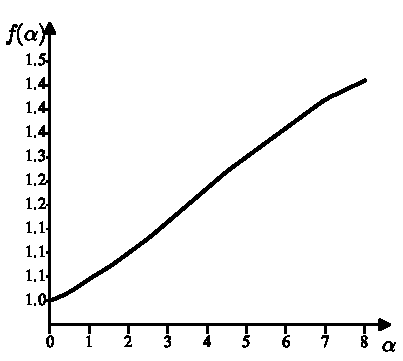
\includegraphics[width=6cm]{fig9-1.pdf}\\{\small 图 9.1\quad $f(\alpha)$曲线}
\end{minipage}
\end{center}

\section{小极化子理论}

在§1中我们已经指出，当电子与LO声子的耦合很强时，电子将被自己产生的极化场束缚，形成局域的极化子状态，其尺寸与晶格常数相近，称为小极化子.显然，对于小极化子问题不能再用连续模型处理，必须从晶格模型出发，同时考虑周期场和电子-LO声子相互作用对载流子（电子或空穴）能态的影响.小极化子在晶格中运动有两种不同方式：其一是能带传导，其二是跳跃过程（hopping processes）.在低温区，小极化子从一格点向邻近格点转移时往往不改变声子组态，在此近似之下系统具有平移对称性，可以形成小极化子的能带状态，它与紧束缚近似中电子的运动相似，不同之处在于计入了晶格振动的影响.涉及到有限温度时非刚性晶格的紧束缚近似能带问题.随着温度升高在小极化子周围的声子数增多，会导致能带传导电子的有效质量增大，从而使极化子带宽变窄.不难想象，存在一个转变温度 $T_{\mathrm t}$，当 $T>T_{\mathrm t}$ 时小极化子的能带宽度将小于它的能量不确定度（$\sim\hbar/\tau$，$\tau$ 是寿命），这时小极化子能带状态不再是系统的定态，极化子的能带图像失效，其运动将改变方式.在高温区小极化子基本上是局域粒子，它只能依靠热声子激活从一格点向另一格点作跳跃运动，与晶格缺陷的扩散运动相似，是一种无规运动并伴随着热声子的产生和消灭（声子组态变化），这种运动方式称为跳跃过程.在本节中我们将采用电子与LO声子耦合的晶格模型\textsuperscript{[13]}来讨论小极化子的能带传导和跳跃过程.

\subsection*{1. 小极化子的哈密顿量}

在三维晶格中电子与LO声子互作用系统由
\begin{equation}
  H=H_{\mathrm e}+H_{\mathrm p}+H_{\mathrm{int}}
\end{equation}
描述，其中
\begin{equation}
  H_{\mathrm e}=\mathscr{E}_{0}\sum_{l}C_{l}^{+}C_{l}
  -J\sum_{l}\sum_{\rho}C_{l+\rho}^{+}C_{l}
\end{equation}
代表电子在晶格周期场中运动的紧束缚近似哈密顿量. $C_{l}$，$C_{l}^{+}$ 是瓦尼尔表象中的电子算符，$\boldsymbol{\rho}$ 代表最近邻格点的位置矢，J为交迭积分，$\mathscr{E}_{0}$ 则代表在任一格点周围分子轨道态能量.
\begin{equation}
  H_{\mathrm p}=\sum_{q}\hbar\omega_{q}
  \biggl(a_{q}^{+}a_{q}+\frac{1}{2}\biggr)
\end{equation}
$a_{q}$、$a_{q}^{+}$ 为LO声子算符，LO声子频率 $\omega_{q}=\omega_{-q}$，具有时间反演对称性.
\begin{equation}
\begin{aligned}
  &H_{\mathrm{int}}=\sum_{q,l}M_{q}\,\mathrm{e}^{\mathrm{i}\boldsymbol{q}\cdot\boldsymbol{l}}
  \bigl(a_{q}+a_{-q}^{+}\bigr)C_{l}^{+}C_{l}\\
  &M_{q}^{*}=M_{-q}
\end{aligned}
\end{equation}
代表晶格模型的电子-LO声子互作用项.式(9.4.4)可仿照第五章§2从瓦尼尔表象导出，其主要步骤如下：

瓦尼尔表象中电子的态矢量
\begin{equation*}
  \varPsi(\boldsymbol{r})=\frac{1}{\sqrt{N}}\sum_{l}C_{l}\,
  a\bigl(\boldsymbol{r}-\boldsymbol{l}\bigr)
\end{equation*}
其中 $a\bigl(\boldsymbol{r}-\boldsymbol{l}\bigr)$ 是瓦尼尔函数.电子-声子互作用的二次量子化表示按常规写成
\begin{equation}
\begin{aligned}
  H_{\mathrm{int}}&=\int\varPsi^{+}(\boldsymbol{r})h(\boldsymbol{r})
  \varPsi(\boldsymbol{r})\,\mathrm{d}\boldsymbol{r}\\
  &=\frac{1}{N}\sum_{l,l'}C_{l}^{+}C_{l}
  \int a^{*}\bigl(\boldsymbol{r}-\boldsymbol{l}'\bigr)h(\boldsymbol{r})
  a\bigl(\boldsymbol{r}-\boldsymbol{l}\bigr)\mathrm{d}\boldsymbol{r}\\
  &\approx\frac{1}{N}\sum_{l}C_{l}^{+}C_{l}
  \int\bigl|a(\boldsymbol{r}-\boldsymbol{l})\bigr|^{2}h(\boldsymbol{r})\,
  \mathrm{d}\boldsymbol{r}
\end{aligned}
\end{equation}
上式的最后一个等号中略去了多中心积分，因为小极化子属于强耦合情况，电子主要是在 $\boldsymbol{l}$ 格点附近的局域轨道上感受到位移的作用.其中 $h(\boldsymbol{r})$ 是晶格位移对单电子作用的势能，对于复式晶格
\begin{equation}
  h(\boldsymbol{r})=-\sum_{l,s}\boldsymbol{u}_{l}(s)\cdot
  \nabla\,v_{s}\bigl(\boldsymbol{r}-\boldsymbol{l}-\boldsymbol{d}_{s}\bigr)
\end{equation}
$\boldsymbol{d}_{s}$ 代表第s原子在元胞中的位置，$v_{s}$ 为原子势，其总和构成晶格周期场
\begin{equation}
  V(\boldsymbol{r})=\sum_{l,s}v_{s}\bigl(\boldsymbol{r}-\boldsymbol{l}
  -\boldsymbol{d}_{s}\bigr)
\end{equation}
复式晶格的位移，根据第二章可写为
\begin{equation}
  \boldsymbol{u}_{l}(s)=\sum_{q,j}
  \sqrt{\frac{\hbar}{2NM_{s}\omega_{qj}}}\,
  \boldsymbol{e}_{qj}\bigl(a_{qj}+a_{-qj}^{+}\bigr)
  \mathrm{e}^{\mathrm{i}\boldsymbol{q}\cdot\boldsymbol{l}}
\end{equation}
其中 $j$ 为声子频谱的支指标.将式(9.4.8)和(9.4.6)代入式(9.4.5)，经整理得到
\begin{equation}
  H_{\mathrm{int}}=\sum_{q,l}\sum_{j}M_{qj}\,
  \mathrm{e}^{\mathrm{i}\boldsymbol{q}\cdot\boldsymbol{l}}
  \bigl(a_{qj}+a_{-qj}^{+}\bigr)C_{l}^{+}C_{l}
\end{equation}
\begin{equation}
  M_{qj}=-\mathrm{i}\sum_{s}
  \sqrt{\frac{\hbar}{2NM_{s}\omega_{qj}}}\,
  \mathrm{e}^{-\mathrm{i}\boldsymbol{q}\cdot\boldsymbol{d}_{s}}v_{s}(\boldsymbol{q})
  \bigl[\boldsymbol{e}_{q}(s)\cdot\boldsymbol{q}\bigr]
  \int\bigl|a(\boldsymbol{r})\bigr|^{2}
  \mathrm{e}^{-\mathrm{i}\boldsymbol{q}\cdot\boldsymbol{r}}\mathrm{d}\boldsymbol{r}
\end{equation}
其中 $v_{s}(\boldsymbol{q})$ 是原子势 $v_{s}(\boldsymbol{r})$ 的傅里叶变换，由关系式
$v_{s}(-\boldsymbol{q})=v_{s}^{*}(\boldsymbol{q})$、$\omega_{-qj}=\omega_{qj}$ 和
$\boldsymbol{e}_{-qj}=\boldsymbol{e}_{qj}^{*}$ 可求得
\begin{equation*}
  \boldsymbol{M}_{-\boldsymbol{q}j}=\boldsymbol{M}_{\boldsymbol{q}j}^{*}
\end{equation*}
如果只考虑LO声子与电子相互作用，则式(9.4.9)中对频谱支指标j的求和可去掉，就得到 $H_{\mathrm{int}}$ 的表示式(9.4.4)了.

\subsection*{2. 位移振子变换}

将 $H_{\mathrm e}$、$H_{\mathrm p}$ 和 $H_{\mathrm{int}}$ 代入式(9.4.1)，小极化子的哈密顿量可重新归并为下列两项之和为
\begin{equation}
  H=H_{0}+H_{1}
\end{equation}
其中
\begin{equation}
  H_{0}=\sum_{l}\biggl\{\mathscr{E}_{0}C_{l}^{+}C_{l}
  +C_{l}^{+}C_{l}\sum_{q}M_{q}\mathrm{e}^{\mathrm{i}\boldsymbol{q}\cdot\boldsymbol{l}}
  \bigl(a_{q}+a_{-q}^{+}\bigr)\biggr\}
  +\sum_{q}\hbar\omega_{q}\bigl(a_{q}^{+}a_{q}+1/2\bigr)
\end{equation}
描述l格点周围局域极化子状态，而
\begin{equation}
  H_{1}=-J\sum_{l,\rho}C_{l+\rho}^{+}C_{l}
\end{equation}
则代表小极化子在晶格中运动项.由于小极化子运动涉及窄能带中载流子迁移问题，其迁移率比较小，可将 $H_{1}$ 当微扰项处理.但是，对于 $H_{0}$ 项，其中包括电子与LO声子的强耦合作用，必须用非微扰方法求解.对于单个极化子问题，可以利用位移振子变换技巧将 $H_{0}$ 对角化，求得局域极化子的本征态.

对H作下列幺正变换：
\begin{equation}
  \overline{H}=\mathrm{e}^{-S}H\mathrm{e}^{S}
  =\overline{H}_{0}+\overline{H}_{1}
\end{equation}
其中母函数S取为
\begin{equation}
  S=\sum_{q,l}\frac{M_{q}}{\hbar\omega_{q}}\,
  \mathrm{e}^{\mathrm{i}\boldsymbol{q}\cdot\boldsymbol{l}}C_{l}^{+}C_{l}
  \bigl(a_{q}+a_{-q}^{+}\bigr)
\end{equation}
变换后的声子算符为
\begin{equation}
\left.
\begin{aligned}
  &\mathrm{e}^{-S}a_{q}\mathrm{e}^{S}=a_{q}
  -\sum_{l}\frac{M_{q}^{*}}{\hbar\omega_{q}}\,
  \mathrm{e}^{-\mathrm{i}\boldsymbol{q}\cdot\boldsymbol{l}}C_{l}^{+}C_{l}\\
  &\mathrm{e}^{-S}a_{q}^{+}\mathrm{e}^{S}=a_{q}^{+}
  -\sum_{l}\frac{M_{q}}{\hbar\omega_{q}}\,
  \mathrm{e}^{\mathrm{i}\boldsymbol{q}\cdot\boldsymbol{l}}C_{l}^{+}C_{l}
\end{aligned}\right\}
\end{equation}
相当于作了原点位移.电子算符 $C_{l}$ 与 $C_{l}^{+}$ 经变换成为
\begin{equation}
\left.
\begin{aligned}
  &\mathrm{e}^{-S}C_{l}\mathrm{e}^{S}=C_{l}X_{l}\\
  &\mathrm{e}^{-S}C_{l}^{+}\mathrm{e}^{S}=C_{l}^{+}X_{l}^{+}
\end{aligned}\right\}
\end{equation}
其中
\begin{equation}
  X_{l}=\exp\biggl\{\sum_{q}\biggl(\frac{M_{q}}{\hbar\omega_{q}}\biggr)
  \mathrm{e}^{\mathrm{i}\boldsymbol{q}\cdot\boldsymbol{l}}
  \bigl(a_{q}-a_{-q}^{+}\bigr)\biggr\}
\end{equation}
它只含声子算符.由于 $M_{-q}^{*}=M_{q}$ 以及 $\omega_{-q}=\omega_{q}$，对于同一格点有算符等式
\begin{equation}
  X_{l}^{+}X_{l}=1
\end{equation}
因此，变换对 $H_{0}$ 中对角项 $C_{l}^{+}C_{l}$ 无影响，只对 $H_{1}$ 有影响.将以上结果代入式(9.4.14)可得
\begin{equation}
  \overline{H}_{1}=-J\sum_{l}\sum_{\rho}'
  C_{l+\rho}^{+}C_{l}X_{l+\rho}^{+}X_{l}
\end{equation}
\begin{equation}
  \overline{H}_{0}=\sum_{l}\bigl(\mathscr{E}_{0}-\Delta\bigr)C_{l}^{+}C_{l}
  +\sum_{q}\hbar\omega_{q}\biggl(a_{q}^{+}a_{q}+\frac{1}{2}\biggr)
  +\sum_{l\neq l'}\sum U\bigl(\boldsymbol{l}-\boldsymbol{l}'\bigr)
  C_{l}^{+}C_{l'}^{+}C_{l'}C_{l}
\end{equation}
上式中右边最后一项代表 $\boldsymbol{l}$ 处与 $\boldsymbol{l}'$ 处两个局域极化子的有效互作用，其中
\begin{equation}
  U\bigl(\boldsymbol{l}-\boldsymbol{l}'\bigr)\equiv
  -\sum_{q}\biggl(\frac{\bigl|M_{q}\bigr|^{2}}{\hbar\omega_{q}}\biggr)
  \mathrm{e}^{\mathrm{i}\boldsymbol{q}\cdot(\boldsymbol{l}-\boldsymbol{l}')}
\end{equation}
它对于双极化子问题的研究有重要作用，在单极化子问题中这一项可以略去，于是求得单个局域极化子的对角化哈密顿量
\begin{equation}
  H_{0}\approx\sum_{l}\bigl(\mathscr{E}_{0}-\Delta\bigr)C_{l}^{+}C_{l}
  +\sum_{q}\hbar\omega_{q}\biggl(a_{q}^{+}a_{q}+\frac{1}{2}\biggr)
\end{equation}
这里
\begin{equation}
  \Delta\equiv\sum_{q}\frac{\bigl|M_{q}\bigr|^{2}}{\hbar\omega_{q}}
\end{equation}
是 $H_{\mathrm{int}}$ 对 $\mathscr{E}_{0}$ 的修正.由 $\overline{H}_{0}$ 描述的l格点局域极化子状态可写成
\begin{equation}
  |1_{l}\rangle\prod_{q}|n_{q}\rangle
  \equiv|1_{l}\rangle\,|\{n_{q}\}\rangle
\end{equation}
$\prod\limits_{q}|n_{q}\rangle$ 是极化子的声子组态，$n_{q}$ 代表 $\boldsymbol{q}$ 波矢的LO声子数.

现在讨论微扰项 $\overline{H}_{1}$ 的作用，利用式(9.4.25)和(9.4.20)，立刻求得小极化从 $\boldsymbol{l}$ 格点向 $\boldsymbol{l}+\boldsymbol{\rho}$ 格点跃迁矩阵元为
\begin{equation*}
  -J\langle f|X_{l+\rho}^{+}X_{l}|i\rangle
\end{equation*}
其中 $|i\rangle=|\{n_{q}\}\rangle$ 和 $|f\rangle=|\{n_{q}'\}\rangle$ 为跃迁前后的声子组态.由于 $X_{l+\rho}^{+}X_{l}$ 允许声子的产生和消灭，因此从态 $|i\rangle$ 向 $|f\rangle$ 跃迁时可能出现两种情况：

（i）对角跃迁：这时 $|i\rangle=|f\rangle$，跃迁前后声子组态不变，可以建立小极化子能带理论.

（ii）非对角跃迁：$|i\rangle\neq|f\rangle$，声子组态发生了改变，从 $\boldsymbol{l}$ 向 $\boldsymbol{l}+\boldsymbol{\rho}$ 跃迁伴随着声子数的变化，属于跳跃运动过程.

下面将分别介绍这两种跃迁过程.

\subsection*{3. 小极化子的能带理论}

如果只发生对角跃迁，小极化子从 $\boldsymbol{l}$ 向 $\boldsymbol{l}+\boldsymbol{\rho}$ 运动时各个 $\boldsymbol{q}$ 态的声子数均无变化，在这样的限制条件下，小极化子在晶格中运动具有平移对称性，可以应用布洛赫定理构成小极化子的能带状态
\begin{equation}
  |1_{k},\{n_{q}\}\rangle=\frac{1}{\sqrt{N}}\sum_{l}
  \mathrm{e}^{\mathrm{i}\boldsymbol{k}\cdot\boldsymbol{l}}|1_{l}\rangle
  \prod_{q}|n_{q}\rangle
\end{equation}
用上述布洛赫态对 $\overline{H}$ 求对角平均，得到 $\{n_{q}\}$ 声子组态的小极化子能带曲线
\begin{equation}
\begin{aligned}
  E_{k}(\{n_{q}\})&=\bigl\langle 1_{k},\{n_{q}\}\bigl|\overline{H}
  \bigr|1_{k},\{n_{q}\}\bigr\rangle\\
  &=\bigl(\mathscr{E}_{0}-\Delta\bigr)
  +\sum_{q}\hbar\omega_{q}\biggl(n_{q}+\frac{1}{2}\biggr)\\
  &\quad-J\sum_{\rho}\mathrm{e}^{-\mathrm{i}\boldsymbol{k}\cdot\boldsymbol{\rho}}
  \prod_{q}\bigl\langle n_{q}\bigl|\exp(\lambda_{q}^{*}a_{q}^{+}
  -\lambda_{q}a_{q})\bigr|n_{q}\bigr\rangle
\end{aligned}
\end{equation}
这里系数
\begin{equation}
  \lambda_{q}\equiv-\left(M_{q}/\hbar\omega_{q}\right)
  \mathrm{e}^{\mathrm{i}\boldsymbol{q}\cdot\boldsymbol{l}}
  \bigl(1-\mathrm{e}^{\mathrm{i}\boldsymbol{q}\cdot\boldsymbol{\rho}}\bigr)
\end{equation}
有限温度T时小极化子能带曲线应由式(9.4.27)对声子部分统计平均得到
\begin{equation}
\begin{aligned}
  E_{k}(T)&=\bigl(\mathscr{E}_{0}-\Delta\bigr)
  +\sum_{q}\hbar\omega_{q}\biggl(\langle n_{q}\rangle_{T}
  +\frac{1}{2}\biggr)\\
  &\quad-J\sum_{\rho}\mathrm{e}^{\mathrm{i}\boldsymbol{k}\cdot\boldsymbol{\rho}}
  \prod_{q}\bigl\langle\exp(\lambda_{q}^{*}a_{q}^{+}-\lambda_{q}a_{q})
  \bigr\rangle_{T}
\end{aligned}
\end{equation}
其中
\begin{equation}
\begin{aligned}
  \langle n_{q}\rangle_{T}
  &=\bigl(1-\mathrm{e}^{-\beta\hbar\omega_{q}}\bigr)
  \sum_{n_{q}=0}^{\infty}n_{q}\bigl(\mathrm{e}^{-\beta\hbar\omega_{q}}\bigr)^{n_{q}}\\
  &=\bigl(\mathrm{e}^{\beta\hbar\omega_{q}}-1\bigr)^{-1}
  \quad\bigl[\beta=\left(k_{\mathrm B}T\right)^{-1}\bigr]\\
  \bigl\langle\exp\bigl(\lambda_{q}^{*}a_{q}^{+}-\lambda_{q}a_{q}\bigr)
  \bigr\rangle_{T}
  &=\mathrm{e}^{-\frac{1}{2}|\lambda_{q}|^{2}}
  \bigl\langle\mathrm{e}^{\lambda_{q}^{*}a_{q}^{+}}
  \mathrm{e}^{-\lambda_{q}a_{q}}\bigr\rangle_{T}\\
  &=\mathrm{e}^{-\frac{1}{2}|\lambda_{q}|^{2}}
  \bigl(1-\mathrm{e}^{-\beta\hbar\omega_{q}}\bigr)\times
\end{aligned}
\end{equation}
\begin{equation}
  \sum_{n,q}^{\infty}\bigl\langle n_{q}\bigl|
  \mathrm{e}^{\lambda_{q}^{*}a_{q}^{+}}\mathrm{e}^{-\lambda_{q}a_{q}}
  \bigr|n_{q}\bigr\rangle\mathrm{e}^{-\beta n_{q}\hbar\omega_{q}}
\end{equation}
这里应用了算符等式
$\mathrm{e}^{\hat{A}+\hat{B}}
=\mathrm{e}^{-\frac{1}{2}[\hat{A},\hat{B}]}\mathrm{e}^{\hat{A}}\mathrm{e}^{\hat{B}}$.利用声子算符于本征态，容易求得下列关系：
\begin{equation}
\begin{aligned}
  &\mathrm{e}^{-\lambda a}|n\rangle=\sum_{p=0}^{\infty}
  \frac{(-\lambda)^{p}}{p!}\,a^{p}|n\rangle
  =\sum_{p=0}^{\infty}\frac{(-\lambda)^{p}}{p!}
  \biggl[\frac{n!}{(n-p)!}\biggr]^{1/2}|n-p\rangle\\
  &\langle n|\mathrm{e}^{\lambda^{*}a^{+}}
  =\sum_{m=0}^{\infty}\frac{(\lambda^{*})^{m}}{m!}
  \biggl[\frac{n!}{(n-m)!}\biggr]^{1/2}\langle n-m|\\
  &\langle n-m|n-p\rangle=\delta_{pm}
\end{aligned}
\end{equation}
由此算出
\begin{equation}
\begin{aligned}
  \bigl\langle n\bigl|\mathrm{e}^{\lambda^{*}a^{+}}
  \mathrm{e}^{-\lambda a}\bigr|n\bigr\rangle
  &=\sum_{m=0}^{n}\frac{(-|\lambda|^{2})^{m}}{(m!)^{2}}\,
  \frac{n!}{(n-m)!}\\
  &=\mathrm{L}_{n}\bigl(|\lambda|^{2}\bigr)
\end{aligned}
\end{equation}
$\mathrm{L}_{n}$ 为拉盖尔（Laguerre）多项式.再利用拉盖尔多项式的生成函数关系
\begin{equation}
  \left(1-Z\right)^{-1}
  \mathrm{e}^{\left[|\lambda|^{2}Z/(Z-1)\right]}
  =\sum_{n=0}^{\infty}\mathrm{L}_{n}\bigl(|\lambda|^{2}\bigr)Z^{n}
\end{equation}
并令
\begin{equation*}
  Z\equiv\mathrm{e}^{-\beta\hbar\omega_{q}}
\end{equation*}
所以
\begin{equation}
  \frac{Z}{Z-1}=\langle n_{q}\rangle_{T}
\end{equation}
可得
\begin{equation}
\begin{aligned}
  \mathrm{e}^{-S_{T}}&\equiv\prod_{q}
  \bigl\langle\exp(\lambda_{q}^{*}a_{q}^{+}-\lambda_{q}a_{q})
  \bigr\rangle_{T}\\
  &=\exp\biggl[-\sum_{q}|\lambda_{q}|^{2}
  \biggl(\langle n_{q}\rangle_{T}+\frac{1}{2}\biggr)\biggr]
\end{aligned}
\end{equation}
因此小极化子能带为
\begin{equation}
  E_{k}(T)=E_{0}(T)-J\sum_{\rho}\mathrm{e}^{-S_{T}}
  \mathrm{e}^{-\mathrm{i}\boldsymbol{k}\cdot\boldsymbol{\rho}}
\end{equation}
其中
\begin{equation}
  E_{0}(T)\equiv\bigl(\mathscr{E}_{0}-\Delta\bigr)
  +\sum_{q}\hbar\omega_{q}\biggl(\langle n_{q}\rangle_{T}
  +\frac{1}{2}\biggr)
\end{equation}
\begin{equation}
\begin{aligned}
  S_{T}&=\sum_{q}|\lambda_{q}|^{2}
  \biggl(\langle n_{q}\rangle_{T}+\frac{1}{2}\biggr)\\
  &=\sum_{q}\biggl\{\frac{|M_{q}|^{2}}{\left(\hbar\omega_{q}\right)^{2}}
  \bigl|1-\mathrm{e}^{-\mathrm{i}\boldsymbol{q}\cdot\boldsymbol{\rho}}\bigr|^{2}
  \biggl(\langle n_{q}\rangle_{T}+\frac{1}{2}\biggr)\biggr\}\\
  &=\sum_{q}\biggl\{2\,\frac{|M_{q}|^{2}}{\left(\hbar\omega_{q}\right)^{2}}
  \sin^{2}\biggl(\frac{\boldsymbol{q}\cdot\boldsymbol{\rho}}{2}\biggr)
  \coth\biggl(\frac{\hbar\omega_{q}}{2k_{\mathrm B}T}\biggr)\biggr\}
\end{aligned}
\end{equation}
这里对 $\boldsymbol{q}$ 求和后 $S_{T}$ 与 $\boldsymbol{\rho}$ 的取向无关，可将 $\mathrm{e}^{-S_{T}}$ 因子从求和号中抽出，最后得到有限温度能带
\begin{equation}
  E_{k}(T)=E_{0}(T)-J\mathrm{e}^{-S_{T}}
  \sum_{\rho}\mathrm{e}^{-\mathrm{i}\boldsymbol{k}\cdot\boldsymbol{\rho}}
\end{equation}
与第八章§10中刚性晶格的紧束缚近似能带相比较，求得小极化子的能带半宽为
\begin{equation}
  ZJ\exp\left(-S_{T}\right)
\end{equation}
由于 $\exp\left(-S_{T}\right)$ 随温度升高减小，因此小极化子的能带宽度随温度升高变窄.这是小极化子能带不同于刚性晶格电子能带的特征.应当注意到，即使在绝对零度时小极化子的能带半宽仍比 $ZJ$ 小，它等于
\begin{equation*}
  ZJ\exp\left(-S_{0}\right)
\end{equation*}
其中
\begin{equation*}
  S_{0}=\frac{1}{2}\sum_{q}
  \frac{\bigl|M_{q}\bigr|^{2}}{\left(\hbar\omega_{q}\right)^{2}}
  \bigl|1-\mathrm{e}^{\mathrm{i}\boldsymbol{q}\cdot\boldsymbol{\rho}}\bigr|^{2}
\end{equation*}
零温带宽变窄效应是由于电子与LO虚声子互作用（通过零点振动）引起极化子有效质量增大所导致.

为了得到小极化子能带理论的成立条件，还必须估计非对角跃迁的作用.既然，对角跃迁给出小极化子的能带状态 $\left(\boldsymbol{k},\{n_{q}\}\right)$，那么计入非对角跃迁必将引起极化子从 $\left(\boldsymbol{k},\{n_{q}\}\right)$ 态向其它态 $\left(\boldsymbol{k}',\{n_{q}'\}\right)$ 的散射.小极化子在某一能带态的平均寿命 $\tau$ 等于总散射概率的倒数，而 $\left(\hbar/\tau\right)$ 则代表小极化处于带状态的能量不确定度.只有当 $\left(\hbar/\tau\right)$ 远远小于能带半宽度时，才能认为小极化子的能带解是系统的稳定状态.反之，小极化子的能带图像就失去意义了，这时必须计算非对角跃迁概率.

\subsection*{4. 小极化子的跳跃运动}

现在讨论小极化子从 $\boldsymbol{l}$ 向 $\boldsymbol{l}+\boldsymbol{\rho}$ 格点运动的非对角跃迁过程，即声子激活跳跃机制.根据含时微扰理论\textsuperscript{[14]}，跃迁概率（定义为每秒跳跃次数）w 与跃迁矩阵元
$\langle f|X_{l+\rho}^{+}X_{l}|i\rangle$ 关系为
\begin{equation}
  w=\frac{1}{\hbar^{2}}\int_{-\infty}^{\infty}\mathrm{d}t\,W(t)
\end{equation}
其中
\begin{equation}
\begin{aligned}
  W(t)&\equiv J^{2}\sum_{f\neq i}
  \bigl\langle i\bigl|X_{l}^{+}(t)X_{l+\rho}(t)\bigr|f\bigr\rangle
  \bigl\langle f\bigl|X_{l+\rho}^{+}X_{l}\bigr|i\bigr\rangle\\
  &=J^{2}\bigl\{\bigl\langle i\bigl|X_{l}^{+}(t)X_{l+\rho}(t)
  X_{l+\rho}^{+}X_{l}\bigr|i\bigr\rangle
  -\bigl|\bigl\langle i\bigl|X_{l+\rho}^{+}X_{l}\bigr|i\bigr\rangle\bigr|^{2}\bigr\}
\end{aligned}
\end{equation}
\begin{equation}
  X_{l}(t)=\mathrm{e}^{\mathrm{i}\overline{H}_{0}t/\hbar}X_{l}
  \mathrm{e}^{-\mathrm{i}\overline{H}_{0}t/\hbar}
\end{equation}
对角跃迁矩阵元为
\begin{equation}
  \bigl\langle i\bigl|X_{l+\rho}^{+}X_{l}\bigr|i\bigr\rangle
  =\prod_{q}\bigl\langle n_{q}\bigl|\exp(\lambda_{q}^{*}a_{q}^{+}
  -\lambda_{q}a_{q})\bigr|n_{q}\bigr\rangle
\end{equation}
其统计平均值为 $\exp\left(-S_{T}\right)$，并在热力学极限近似用 $\exp\left(-2S_{T}\right)$ 表示
$\bigl|\langle i|X_{l+\rho}^{+}X_{l}|i\rangle\bigr|^{2}$，由式(9.4.18)和(9.4.28)求得W中的时间关联函数
\begin{equation}
\begin{aligned}
  &\bigl\langle i\bigl|X_{l}^{+}(t)X_{l+\rho}(t)X_{l+\rho}^{+}X_{l}
  \bigr|i\bigr\rangle\\
  &\quad=\bigl\langle i\bigl|\exp\biggl\{\sum_{q}\biggl[
  \biggl(\lambda_{q}a_{q}+\frac{1}{2}\bigl|\lambda_{q}\bigr|^{2}\biggr)
  \bigl(\mathrm{e}^{-\mathrm{i}\omega_{q}t}-1\bigr)\\
  &\qquad-\biggl(\lambda_{q}^{*}a_{q}^{+}
  +\frac{1}{2}\bigl|\lambda_{q}\bigr|^{2}\biggr)
  \bigl(\mathrm{e}^{\mathrm{i}\omega_{q}t}-1\bigr)\biggr]\biggr\}
  \biggr|i\bigr\rangle\\
  &\quad=\exp\biggl[-\frac{1}{2}\sum_{q}B_{q}\biggr]\prod_{q}
  \bigl\langle n_{q}\bigl|\exp\bigl(A_{q}^{*}a_{q}^{+}-A_{q}a_{q}\bigr)
  \bigr|n_{q}\bigr\rangle
\end{aligned}
\end{equation}
其中 $\lambda_{q}$ 由式(9.4.28)定义，而
\begin{equation*}
\begin{aligned}
  &A_{q}\equiv-\lambda_{q}\bigl(\mathrm{e}^{-\mathrm{i}\omega_{q}t}-1\bigr)\\
  &B_{q}\equiv|\lambda_{q}|^{2}
  \bigl[\bigl(\mathrm{e}^{\mathrm{i}\omega_{q}t}-1\bigr)
  -\bigl(\mathrm{e}^{-\mathrm{i}\omega_{q}t}-1\bigr)\bigr]
\end{aligned}
\end{equation*}
式(9.4.46)中含声子算符 $a_{q}$ 与 $a_{q}^{+}$ 部分的统计平均为
\begin{equation*}
  \prod_{q}\bigl(1-\mathrm{e}^{-\beta\hbar\omega_{q}}\bigr)
  \sum_{n_{q}=0}^{\infty}\bigl(\mathrm{e}^{-\beta\hbar\omega_{q}}\bigr)^{n_{q}}
  \bigl\langle n_{q}\bigl|\mathrm{e}^{A_{q}^{*}a_{q}^{+}-A_{q}a_{q}}
  \bigr|n_{q}\bigr\rangle
\end{equation*}
作类似于上节的计算，利用式(9.4.36)求得
\begin{equation}
  \bigl\langle X_{l}^{+}(t)X_{l+\rho}(t)X_{l+\rho}^{+}X_{l}
  \bigr\rangle_{T}
  =\exp\{-2S_{T}+\varphi(t)\}
\end{equation}
其中 $S_{T}$ 由式(9.4.39)决定，而
\begin{equation}
\begin{aligned}
  \varphi(t)&=\sum_{q}|\lambda_{q}|^{2}
  \bigl\{\bigl(\langle n_{q}\rangle_{T}+1\bigr)
  \mathrm{e}^{-\mathrm{i}\omega_{q}t}
  +\langle n_{q}\rangle_{T}\mathrm{e}^{\mathrm{i}\omega_{q}t}\bigr\}\\
  &=2\sum_{q}|\lambda_{q}|^{2}
  \bigl[\langle n_{q}\rangle_{T}\bigl(\langle n_{q}\rangle_{T}+1\bigr)
  \bigr]^{1/2}
  \cos\biggl[\omega_{q}\biggl(t+\frac{\mathrm{i}\beta\hbar}{2}\biggr)\biggr]
\end{aligned}
\end{equation}
其中利用了下列关系式：
\begin{equation*}
  \sqrt{\frac{\langle n_{q}\rangle_{T}+1}{\langle n_{q}\rangle_{T}}}
  =\mathrm{e}^{\frac{1}{2}\beta\hbar\omega_{q}}\,,\quad
  \sqrt{\frac{\langle n_{q}\rangle_{T}}{\langle n_{q}\rangle_{T}+1}}
  =\mathrm{e}^{-\frac{1}{2}\beta\hbar\omega_{q}}
\end{equation*}
将式(9.4.48)代入式(9.4.43)和(9.4.42)，可得w的统计平均值为
\begin{equation}
  w_{T}=\frac{J^{2}}{\hbar^{2}}\mathrm{e}^{-2S_{T}}
  \int_{-\infty}^{\infty}\mathrm{d}t\,
  \bigl(\mathrm{e}^{\varphi(t)}-1\bigr)
\end{equation}
在三维情况下被积函数收敛很快，可将 $\varphi(t)$ 延拓到 t 的复平面z上成为
\begin{equation}
  \varphi(z)=2\sum_{q}|\lambda_{q}|^{2}
  \bigl[\langle n_{q}\rangle_{T}
  \bigl(\langle n_{q}\rangle_{T}+1\bigr)\bigr]^{1/2}
  \cos\omega_{q}z
\end{equation}
在 $z=0$ 附近展开 $\varphi(z)$，得
\begin{equation*}
  \varphi(z)\approx\varphi(0)-\gamma z^{2}+\cdots,
\end{equation*}
\begin{equation}
  \varphi(0)=2\sum_{q}|\lambda_{q}|^{2}
  \bigl[\langle n_{q}\rangle_{T}
  \bigl(\langle n_{q}\rangle_{T}+1\bigr)\bigr]^{1/2}
\end{equation}
\begin{equation}
  \gamma=\sum_{q}\omega_{q}^{2}|\lambda_{q}|^{2}
  \bigl[\langle n_{q}\rangle_{T}
  \bigl(\langle n_{q}\rangle_{T}+1\bigr)\bigr]^{1/2}
\end{equation}
代入式(9.4.49)作回路积分\textsuperscript{[13]}
\begin{equation}
\begin{aligned}
  w_{T}&=\frac{J^{2}}{\hbar^{2}}\mathrm{e}^{-2S_{T}}
  \int\mathrm{d}z\,\bigl(\mathrm{e}^{\varphi(z)}-1\bigr)\\
  &\approx\frac{J^{2}}{\hbar^{2}}
  \biggl\{\int_{-\infty}^{\infty}\mathrm{d}z\,\mathrm{e}^{-\gamma z^{2}}
  \biggr\}\exp\bigl[-2S_{T}+\varphi(0)\bigr]\\
  &\approx\frac{J^{2}}{\hbar^{2}}
  \biggl(\frac{\pi}{\gamma}\biggr)^{\frac{1}{2}}
  \exp\bigl[-2S_{T}+\varphi(0)\bigr]
\end{aligned}
\end{equation}
再将 $\langle n_{q}\rangle_{T}$ 和 $\lambda_{q}$ 代入 $S_{T}$ 及 $\varphi(0)$ 中，在高温近似下求出
\begin{equation}
\begin{aligned}
  2S_{T}-\varphi(0)&=\sum_{q}\frac{|M_{q}|^{2}}
  {\left(\hbar\omega_{q}\right)^{2}}
  \bigl|1-\mathrm{e}^{\mathrm{i}\boldsymbol{q}\cdot\boldsymbol{\rho}}\bigr|^{2}
  \bigl\{\bigl(2\langle n_{q}\rangle_{T}+1\bigr)\\
  &\quad-2\bigl[\langle n_{q}\rangle_{T}
  \bigl(\langle n_{q}\rangle_{T}+1\bigr)\bigr]^{1/2}\bigr\}\\
  &\approx\sum_{q}\frac{|M_{q}|^{2}}{\left(\hbar\omega_{q}\right)^{2}}
  \bigl|1-\mathrm{e}^{\mathrm{i}\boldsymbol{q}\cdot\boldsymbol{\rho}}\bigr|^{2}
  \frac{\hbar\omega_{q}}{4k_{\mathrm B}T}
\end{aligned}
\end{equation}
定义一个能量
\begin{equation}
  E_{\mathrm a}\equiv\frac{1}{4}\sum_{q}
  \biggl(\frac{|M_{q}|}{\hbar\omega_{q}}\biggr)^{2}
  \bigl|1-\mathrm{e}^{\mathrm{i}\boldsymbol{q}\cdot\boldsymbol{\rho}}\bigr|^{2}
  \hbar\omega_{q}
\end{equation}
在高温近似下由式(9.4.52)求得
\begin{equation}
  \gamma\approx\frac{4E_{\mathrm a}k_{\mathrm B}T}{\hbar^{2}}
\end{equation}
最后得到小极化子跳跃概率的高温近似式
\begin{equation}
  w_{T}=\biggl(\frac{J}{\hbar}\biggr)^{2}
  \biggl(\frac{\pi\hbar^{2}}{4E_{\mathrm a}k_{\mathrm B}T}\biggr)^{\frac{1}{2}}
  \exp\biggl(-\frac{E_{\mathrm a}}{k_{\mathrm B}T}\biggr)
\end{equation}
它随温度升高而增大，说明小极化子靠声子热激活在晶格中作无规运动，$E_{\mathrm a}$ 可理解为跳跃运动的激活能.对于简立方晶格小极化子的扩散系数
\begin{equation}
  D=a^{2}w_{T}=\biggl(\frac{Ja}{\hbar}\biggr)^{2}
  \sqrt{\frac{\pi\hbar^{2}}{4E_{\mathrm a}k_{\mathrm B}T}}\,
  \exp\biggl(-\frac{E_{\mathrm a}}{k_{\mathrm B}T}\biggr)
\end{equation}
这里a为晶格常数.小极化子的跳跃迁移率可根据爱因斯坦关系决定
\begin{equation}
  \mu=\frac{eD}{k_{\mathrm B}T}
  =\frac{ea^{2}}{k_{\mathrm B}T}\,w_{T}
  \sim\exp\biggl(-\frac{E_{\mathrm a}}{k_{\mathrm B}T}\biggr)
\end{equation}
迁移率随温度升高而增大与晶格缺陷运动完全相似，因此人们常称小极化子状态称为晶体的一种“本征缺陷”.

\subsection*{5. 两种导电机制的转变温度$T_{\mathrm t}$}

实际上小极化子在某能带态上的寿命 $\tau$ 就是非对角跃迁概率 $w_{T}$ 的倒数.由于每个格点有z个近邻，因此 $z\hbar w_{T}$ 确定小极化子带状态的能量不确定度.当能带半宽满足条件
\begin{equation}
  J\exp\left(-2S_{T}\right)\gg\hbar w_{T}
\end{equation}
时，非对角跃迁可忽略，小极化子能带理论成立.由于 $T\to0$ K时 $w_{T}\to0$，因此低温区小极化子按能带传导方式在晶格中运动，其导电率随温度升高而降低.反过来，当T升高 $w_{T}$ 增大而 $\mathrm{e}^{-2S_{T}}$ 减小以致满足下列条件时，
\begin{equation}
  \hbar w_{T}\gg J\exp\left(-2S_{T}\right)
\end{equation}
非对角跃迁起主要作用，这时小极化子在晶格中作无规跳跃运动，其导电率随T升高增大.因此划分小极化子导电机制的转变温度应由下列等式决定：
\begin{equation*}
  \hbar w_{T_{\mathrm t}}=J\exp\left(-2S_{T_{\mathrm t}}\right)
\end{equation*}
由于 $T_{\mathrm t}$ 在中间温区，$w_{T}$ 的高温近似结果［式(9.4.57)］不能应用.文献[15]的详细计算表明，当 $\hbar\omega_{\mathrm D}/J$ 在1到100之间时，$T_{\mathrm t}$ 在 $0.4\theta_{\mathrm D}$ 到 $0.55\theta_{\mathrm D}$ 之间.这里 $\theta_{\mathrm D}$ 和 $\omega_{\mathrm D}$ 分别为德拜温度和频率.实验上也观测到了这种转变，例如 TiO$_{2}$ 的 $T_{\mathrm t}$ 大致为300℃\textsuperscript{[16]}.

现已证实，在新发现的混合价锰氧化物
$\mathrm{Re}_{1-x}\mathrm{A}_{x}\mathrm{MnO}_{3}$
（Re：La，Nd；A：Ca，Sr）组成的庞磁电阻（colossal magnetoresistance，CMR）系统中，小极化子的高温跳跃传导\textsuperscript{[17]}和低温能带传导\textsuperscript{[18]}均起重要作用.

\section{一维极化子理论}

近年来由于低维系统非线性元激发的研究进展，重新引起人们对一维极化子理论的兴趣.例如，在聚乙炔链中不仅发现了扭形孤子解，成功地预言了“分数电荷”等特殊自旋-电荷关系\textsuperscript{[19]}，而且还找到了非线性的孤波型极化子解，并成功地说明了聚乙炔中的晶格弛豫现象\textsuperscript{[20]}.这类极化子解实质上是准一维聚乙炔链中电子与LO声子相互作用所形成的自陷态，它和一维分子晶体中的局域极化子状态有密切的关系\textsuperscript{[21,22]}.因此有必要对一维极化子的分子晶体模型\textsuperscript{[15]}作简单介绍.

设系统中包含一个过剩电子和由N个双原子分子组成的线性链.每个分子对电子作用的势能设为 $U\bigl(x-R_{n},u_{n}\bigr)$，其中 $R_{n}=na$ 代为第n个分子的位置，$u_{n}$ 是第n个分子中原子间相对振动的位移，这就是分子晶体模型.根据这个模型一维极化子的哈密顿量可写成
\begin{equation}
  H=H_{\mathrm e}+H_{\mathrm p}+H_{\mathrm{int}}
\end{equation}
其中
\begin{equation}
  H_{\mathrm e}+H_{\mathrm{int}}
  =-\frac{\hbar^{2}}{2m}\frac{\mathrm{d}^{2}}{\mathrm{d}x^{2}}
  +\sum_{n=1}^{N}U\bigl(x-R_{n},u_{n}\bigr)
\end{equation}
\begin{equation}
  H_{\mathrm p}=\sum_{n=1}^{N}\biggl(
  -\frac{\hbar^{2}}{2M}\frac{\partial^{2}}{\partial u_{n}^{2}}
  +\frac{1}{2}M\omega_{0}^{2}u_{n}^{2}
  +\frac{1}{2}M\omega_{1}^{2}u_{n}u_{n+1}\biggr)
\end{equation}
M代表相对分子质心运动的折合质量，$\omega_{0}^{2}$ 与 $\omega_{1}^{2}$ 则相当于第二章中动力矩阵的“对角”与“非对角”元素，在这里只计及了分子间近邻互作用.从物理上讲，$\omega_{0}$ 代表爱因斯坦频率，$\omega_{1}^{2}u_{n}u_{n+1}$ 项则给出LO晶格振动频率的色散部分.

哈密顿量H的波函数假定为下列线性组合
\begin{equation}
  \varPsi=\sum_{n}a_{n}\bigl(u_{1},\cdots,u_{N}\bigr)
  \phi_{n}\bigl(x,u_{n}\bigr)
\end{equation}
其中 $\phi_{n}$ 为局域化的分子轨道，它满足方程
\begin{equation}
  \biggl\{-\frac{\hbar^{2}}{2m}\frac{\mathrm{d}^{2}}{\mathrm{d}x^{2}}
  +U\bigl(x-R_{n},u_{n}\bigr)\biggr\}
  \phi_{n}\bigl(x-R_{n},u_{n}\bigr)
  =E\bigl(u_{n}\bigr)\phi_{n}\bigl(x-R_{n},u_{n}\bigr)
\end{equation}
由于各分子结构相同，因此分子轨道的本征值E只与分子振动的位移量 $u_{n}$ 有关.在线性近似范围内可将E按 $u_{n}$ 展开写为
\begin{equation*}
  E\bigl(u_{n}\bigr)=-Au_{n}+\mathrm{const.}
\end{equation*}
其中 $-Au_{n}$ 实际上代表电子与晶格振动的相互作用，因为几乎所有的电子-声子互作用都是在类似的线性展开下导出的.适当选取能量的零点，可令上式中常量项为零，于是
\begin{equation}
  E\bigl(u_{n}\bigr)=-Au_{n}
\end{equation}
式(9.5.4)中 $a_{n}\bigl(u_{1},\cdots,u_{N}\bigr)$ 是电子在n格点周围分子轨道上的概率振幅，与紧束缚近似法中的展开系数相似，不同之处在于 $a_{n}$ 随晶格振动的位形 $\left(u_{1},\cdots,u_{N}\right)$ 变化，因为现在所处理的不是刚性晶格.此外 $a_{n}$ 还是时间t的函数，下标n是代表电子状态的量子数，在这里就是格点的位标.

利用与紧束缚近似相类似的作法，可以从薛定谔方程 $\mathrm{i}\hbar\dot{\varPsi}=H\varPsi$ 导出 $a_{n}$ 的运动方程
\begin{equation}
\begin{aligned}
  \mathrm{i}\hbar\frac{\partial}{\partial t}
  a_{n}\bigl(u_{1},\cdots,u_{N}\bigr)
  &=\bigl(H_{\mathrm p}-Au_{n}\bigr)
  a_{n}\bigl(u_{1},\cdots,u_{N}\bigr)\\
  &\quad+\sum_{(\pm)}J\bigl(u_{n},u_{n\pm1}\bigr)
  a_{n\pm1}\bigl(u_{1},\cdots,u_{N}\bigr)
\end{aligned}
\end{equation}
其中
\begin{equation}
  J\bigl(u_{n},u_{m}\bigr)=\int\phi^{*}
  \bigl(\boldsymbol{x}-\boldsymbol{R}_{n},u_{n}\bigr)
  U\bigl(\boldsymbol{x}-\boldsymbol{R}_{n},u_{n}\bigr)
  \phi\bigl(\boldsymbol{x}-\boldsymbol{R}_{m},u_{m}\bigr)
  \mathrm{d}\boldsymbol{x}
\end{equation}
是双中心交迭积分.在推导过程中略去了三中心积分，只保留最近邻的双中心交迭积分.此外，还略去了 $\phi$ 对 $u_{n}$ 的导数项，文献[21]中证明了这一项作用不大，略去它相当于作绝热近似.如再略去J对u的依赖关系设 $J\bigl(u_{n},u_{n\pm1}\bigr)=-J$，并采用单频近似取 $\omega_{1}=0$，相当于用爱因斯坦模型描述LO声子，则式(9.5.7)可改写成
\begin{equation}
\begin{aligned}
  \mathrm{i}\frac{\partial}{\partial t}
  a_{n}\bigl(u_{1},\cdots,u_{N}\bigr)
  &=\sum_{m}\biggl(-\frac{\hbar^{2}}{2M}
  \frac{\partial^{2}}{\partial u_{m}^{2}}
  +\frac{1}{2}M\omega_{0}^{2}u_{m}^{2}\biggr)
  a_{n}\bigl(u_{1},\cdots,u_{N}\bigr)\\
  &\quad-J\bigl(a_{n+1}+a_{n-1}\bigr)
  -Au_{n}a_{n}\bigl(u_{1},\cdots,u_{N}\bigr)
\end{aligned}
\end{equation}
上式对任意位形 $\left(\boldsymbol{u}_{1},\cdots,\boldsymbol{u}_{N}\right)$ 求解比较困难.在强耦合情况下，电子引起晶格畸变，产生一个吸引势作用于电子本身，使电子陷落在势阱中形成自陷态，而自陷态的出现又使晶格畸变得以保持.因此，起主要作用的是晶格的静态位移，这时晶格振动的动能项对 $a_{n}$ 的影响不大，可以忽略不计.这相当于对 $a_{n}\bigl(u_{1},\cdots,u_{N}\bigr)$ 作绝热近似，并设 $a_{n}$ 有定态解，其能量本征值为 $E\bigl(u_{1},\cdots,u_{N}\bigr)$.这时式(9.5.9)简化为下列本征方程：
\begin{equation}
  \biggl\{\frac{1}{2}\sum_{m}M\omega_{0}^{2}u_{m}^{2}-Au_{n}\biggr\}a_{n}
  -J\bigl(a_{n+1}+a_{n-1}\bigr)
  =E\bigl(u_{1},\cdots,u_{N}\bigr)a_{n}
\end{equation}
将上式对 $a_{n}$ 求内积，并利用归一化条件
\begin{equation}
  1=\int|\varPsi|^{2}\mathrm{d}x=\sum_{n}|a_{n}|^{2}
\end{equation}
可求出 $E\bigl(u_{1},\cdots,u_{N}\bigr)$.系统的基态可以从 $E\bigl(u_{1},\cdots,u_{N}\bigr)$ 对 $u_{m}$ 的变分极值决定，不难算得能量极小时振动位移
$\bigl(u_{1}^{(0)},\cdots,u_{N}^{(0)}\bigr)$ 满足
\begin{equation}
  u_{m}^{(0)}=A\bigl|a_{m}^{(0)}\bigr|^{2}/M\omega_{0}^{2}
  \quad\left(m=1,2,\cdots,N\right)
\end{equation}
其中 $a_{m}^{(0)}$ 代表 $u_{m}=u_{m}^{(0)}$ 时式(9.5.10)的解.将式(9.5.12)代入式(9.5.10)，求得 $a_{n}^{(0)}$ 的方程为
\begin{equation}
  \biggl\{\frac{A^{2}}{M\omega_{0}^{2}}
  \bigl|a_{n}^{(0)}\bigr|^{2}-\mathscr{E}\biggr\}a_{n}^{(0)}
  +J\bigl(a_{n+1}^{(0)}+a_{n-1}^{(0)}-2a_{n}^{(0)}\bigr)=0
\end{equation}
其中
\begin{equation}
  \mathscr{E}\equiv\left(1/2\right)\sum_{m}M\omega_{0}^{2}
  u_{m}^{(0)2}
  -E\bigl(u_{1}^{(0)},\cdots,u_{N}^{(0)}\bigr)-2J
\end{equation}
当 $a_{n}^{(0)}$ 是n的缓变函数时，可作下列连续化近似：
\begin{equation}
  a_{n+1}^{(0)}+a_{n-1}^{(0)}-2a_{n}^{(0)}
  \approx\frac{\partial^{2}a_{n}^{(0)}}{\partial n^{2}}
\end{equation}
再定义参数
\begin{equation}
  \gamma\equiv A^{2}/4M\omega_{0}^{2}J
\end{equation}
可将 $a_{n}^{(0)}$ 的方程式(9.5.13)写成下列非线性定态薛定谔方程：
\begin{equation}
  \frac{\mathrm{d}^{2}a_{n}^{(0)}}{\mathrm{d}n^{2}}
  +4\gamma\bigl|a_{n}^{(0)}\bigr|^{2}a_{n}^{(0)}
  =\biggl(\frac{\mathscr{E}}{J}\biggr)a_{n}^{(0)}
\end{equation}
考虑方程在 $n\rightarrow\pm\infty$ 时 $a_{n}^{(0)}$ 及其导数趋向零的解，它代表极化子局域状态.这个解很容易直接求出，只要对式(9.5.17)乘以 $2\left(\mathrm{d}a_{n}/\mathrm{d}n\right)$，立刻可将上式变换为全微分，并求得其严格解为
\begin{equation}
  a_{n}^{(0)}=\sqrt{\frac{\mathscr{E}}{2\gamma J}}\,
  \mathrm{sech}\sqrt{\frac{\mathscr{E}}{J}}\,
  \left(n-n_{0}\right)
\end{equation}
其中 $n_{0}$ 是积分常数. $\mathscr{E}$ 可由归一化条件
$\sum\limits_{n}\bigl|a_{n}^{(0)}\bigr|^{2}=1$ 定出
\begin{equation}
  \mathscr{E}=J\gamma^{2}
\end{equation}
代入式(9.5.14)求得
\begin{equation}
  E\bigl(u_{1}^{(0)},\cdots,u_{N}^{(0)}\bigr)
  =-\left(1/3\right)J\gamma^{2}-2J
\end{equation}
由于2J为刚性晶格的紧束缚近似能带半宽.因此上式右边第二项-2J为能带底部电子的能量，这是周期场所造成的，而第一项则代表形成局域极化子状态时所降低的能量，因此极化子的束缚能
\begin{equation}
  E_{\mathrm p}=\frac{1}{3}J\gamma^{2}
  =\frac{1}{48J}\biggl(\frac{A^{2}}{M\omega_{0}^{2}}\biggr)^{2}
\end{equation}
局域极化子状态（即自陷态）中的晶格位移由式(9.5.18)和(9.5.12)决定：
\begin{equation}
  u_{n}^{(0)}=\frac{A}{2M\omega_{0}^{2}}\gamma\,
  \mathrm{sech}^{2}\bigl[\gamma\left(n-n_{0}\right)\bigr]
\end{equation}
相应的电子自陷势阱则为
\begin{equation}
\begin{aligned}
  V\bigl(u_{n}^{(0)}\bigr)&=E\bigl(u_{n}^{(0)}\bigr)=-Au_{n}^{(0)}\\
  &=-\frac{A^{2}}{2M\omega_{0}^{2}}\gamma\,
  \mathrm{sech}^{2}\bigl[\gamma\left(n-n_{0}\right)\bigr]
\end{aligned}
\end{equation}
根据式(9.5.18)和(9.5.19)可定出局域极化子的概率振幅：
\begin{equation}
  a_{n}^{(0)}=\sqrt{\frac{\gamma}{2}}\,
  \mathrm{sech}\bigl[\gamma\left(n-n_{0}\right)\bigr]
\end{equation}
若定义
\begin{equation}
  L_{\mathrm p}\equiv\frac{a}{\gamma}
  =\biggl(\frac{4M\omega_{0}^{2}J}{A^{2}}\biggr)a
\end{equation}
可将 $a_{n}^{(0)}$ 用 $L_{\mathrm p}$ 表示为
\begin{equation}
  a_{n}^{(0)}=\sqrt{\frac{a}{2L_{\mathrm p}}}\,
  \mathrm{sech}\biggl[\frac{\left(n-n_{0}\right)a}{L_{\mathrm p}}\biggr]
\end{equation}
其中 $\boldsymbol{a}$ 为晶格常数.显而易见，上式描述一个峰值在 $n_{0}a$ 处的钟形峰，其峰宽 $L_{\mathrm p}$ 代表极化子的尺寸.当 $L_{\mathrm p}\gg a$ 时，称为大极化子，反之当 $L_{\mathrm p}\leqslant a$ 时是小极化子.由于这个极化子解与包络孤子解十分相似，人们又称其为孤波型极化子解，聚乙炔中的极化子解与上述极化子解的物理实质是相同的，具体的差异在文献[18]中作了详细比较.

\begin{canKao}
\begin{enumerate}[label={[\arabic*]}, leftmargin=2.2em, itemsep=0pt]
\item Lee T D, Low F E, Pines D. Phys Rev, 1953, 90: 297
\item Pines D, Kuper C G, Whitefield G D eds. Polarons and Excitons. New York: Plenum Press. 1963
\item Haeringen W V. Phys Rev, 1965, 137: A1902
\item 程开甲，李正中. 科学通报（研究栏），1958，6：186
\item Tiablikov S V. Sov Phys Solid State, 1962, 3: 2500
\item Gross E P. Phys Rev, 1955, 100: 1571
\item Feynman R P. Phys Rev, 1955, 97: 660
\item Apple J. Solid State Physics, 1968, 21: 193
\item Mitra TK et al. Phys. Rep. 1987, 153, 91; Devreese JT. Encyclopedia of Applied Physics. New York: VCH Publishers. 1996, 14: 383
\item Low F E. Phys Rev, 1955, 97: 1392
\item Chew G F, Low F E. Phys Rev, 1956, 101: 1570
\item Low F E, Pines D. Phys Rev, 1955, 98: 414
\item Mahan G D. Many Particle Physics. New York: Plenum Press, 1981
\item Schiff L I. Quantum Mechanics (2nd ed). New York: McGraw-Hill, 1955. 199
\item Holstein T. Ann Phys, 1959, 8: 325, 343
\item Bogomolov V N et al. Sov Phys Solid State, 1968, 9: 2502
\item 沈瑞，李正中. Solid State Commun，1999，110：237
\item Zhao G M et al. Phys Rev Lett, 2000, 84: 6068
\item Su W P, Schrieffer J R, Heeger A J. Phys Rev, 1980, B22: 2099
\item Su Z B, Yu L. Phys Rev, 1983, B27: 5199
\item Campell D K et al. Phys Rev, 1982, B26: 6862
\item Holstein T. Mol. Cryst Liq Cryst, 1981, 77: 235
\end{enumerate}
\end{canKao}

% ============================================================
%  第十章 激子理论（§1–§5 + 章末参考文献）
%  底本：高等教育出版社《固体理论》第二版；原书印刷页 369–389
%  （PDF 页 = 印刷页 + 20）
%  公式编号自检：§2 (10.2.1)–(10.2.11)；§3 (10.3.1)–(10.3.17)；
%    §4 (10.4.1)–(10.4.50)；§5 (10.5.1)–(10.5.16)。
%    全章自动编号 94 个，无缺号（任务单 tags=92 系 OCR 丢
%    (10.3.16)（积分 I 式）之号并把 (10.4.27) 整式乱码所致，
%    均已对照原书页面补排，见下）。
%
%  任务单所列"缺号"逐条对照原书页面判定（均非原书跳号）：
%    (10.3.16) 积分 I 式：OCR 丢号留式，原书 p374 在号（编号
%              印于式下），OCR 把下一式误标为 10.3:16；
%    (10.3.17) 原书 p374 在号（编号嵌于式旁，OCR 误识为式内
%              文字）；
%    (10.4.27) 整式 OCR 乱码，按 p378 原书五行等式逐行复原；
%    (10.4.28) OCR tag 残缺为 0.4.28 且整式乱码，按 p378 复原；
%    (10.4.34)(10.4.35)(10.4.36) OCR tag 残缺，公式原书均在
%              （p379–380）。
%
%  已修正的 OCR/原书错误（除全角句点转"."、删 ~ 间隔符、收紧
%  \mathrm{d}、拆开行内公式与中文、修复被拆散的函数名等常规项外）：
%  1. §1 段首"禁带宽度"OCR 乱码 $\cal E_s$ 按原书 p369 复原为 E_g。
%  2. §3 (10.3.1)(10.3.6) OCR 之 \bar\Phi_0、\bar\Phi_n 的横线
%     系 OCR 噪声，原书 p372–373 无横线，删。
%  3. (10.3.7) 第二行系数原书印 1/2，按上下文应为 1/N
%     （由 |Ψ_K> 归一推导及 (10.3.8) 之系数一致性），已改 1/N
%     并在此注明：原书误印 1/2。
%  4. (10.3.8)(10.3.13) 求和号上的撇号（排除 R_nm=0 项）照原书
%     用 \sum' 复原（OCR 乱码 \stackrel{*}{=}、\et{}{'}）。
%  5. §3 末段"它代表 K→0 时"OCR 缺箭头，按 p374 补 $\to$。
%  6. (10.4.2) 第二行第一个产生算符原书印 Ψ⁺(r′)，按二次量子化
%     标准形式（与 h 项及消灭算符次序一致）应为 Ψ⁺(r)，
%     已改并注明：原书误印 r′。
%  7. (10.4.16) OCR 乱码"dH/de − E_e|de>"按 p376 复原为
%     0 = (H − E_e)|e>。
%  8. (10.4.21) OCR 之 \mathcal{S}_{k'k} 按原书 p377 复原为
%     δ_{k'k}。
%  9. (10.4.24)(10.4.26) OCR 之"F d("、"R_r"等乱码按 p377–378
%     复原为 F(R_{l'})、R_{l'}；(10.4.26) 首行求和指标按原书
%     为 Σ_{k'}𝓔_ν(k')。
% 10. (10.4.27) 第四个等式首因子原书印 a*_ν(r′−R_1)，按其第三
%     等式及 (10.4.30) 应为 a*_ν(r−R_1)，已改并注明：原书误印 r′。
% 11. (10.4.28) ≈ 行指数原书印 exp{iK·(R_1−R_2)}，按其第二行
%     相位（R_3=R_1、R_4=R_2 代入得 −iK·(R_1−R_2)）及末行
%     e^{−iK·R_12}W(R_12)，应为 exp{−iK·(R_1−R_2)}，已改并注明：
%     原书漏印负号。
% 12. §4.3 末段 OCR"式(10.4.25)与瓦尼尔-莫特激子方程(10.2.5)
%     相同"系原书 p381 误印，所指为式(10.4.45)（同段下文
%     "在推导式(10.4.45)时"可证），已改。
% 13. (10.4.50) 前文 W_K 定义 OCR 印 exp[iK·R_m]，与 (10.4.28)
%     末行及式(10.4.50)之 e^{−iK·R_m} 相矛盾，按 p378–382 统一
%     为 exp[−iK·R_m]（原书 p382 误印 +i）。
% 14. (10.5.3) φ_b(2)≡π^{-1/2}exp(−r_2a)：按 (10.5.2) 配对及
%     下文"其中 r_1a, r_2b, …"应为 exp(−r_2b)，已改并注明：
%     原书误印 r_2a。
% 15. §5"双激子具有类波色子特征"原书误印"波色子"（同段下文
%     即作"玻色凝聚"），改"玻色子"。
% 16. §5"Insb、InAs、GaAs"原书误印 Insb，改 InSb。
% 17. (10.5.11) 原书印 3e²k_F²/2π，k_F 应为一次幂（量纲；与
%     = −1.832/r_s 一致，k_F=(9π/4)^{1/3}/(a_ex r_s)），已改并注明。
% 18. "M̄ 是电子-空穴对的拆合质量"原书误印"拆合"（p374 同语
%     作"折合质量"），改"折合质量"。
% 19. 原书 p388 误印"所得的 E_G(r_s) 曲线如图9.6中虚线所示"，
%     实指图10.6（同页"E-H 液体的基态能的计算曲线"），已改。
% 20. §5 末段 OCR 衍出之 n_0（"E-H液体中 n_0 将分离出…"）系
%     串位，按 p388 原文删；"研究[4,5].．"双句点删一。
% 21. §3"H 的非对角阵矩元为"原书误印"阵矩"，改"矩阵"。
% 22. 文献照录 p389（[11]"Virgina: Spring-field"、[12]"1976,
%     28: 961"原书如此，未改）。
%  插图：图 10.1 激子能级（p371）、图 10.2 局域激发态（p372）、
%  图 10.3 积分 I 的计算图（p374）、图 10.4 双激子互作用（p384）、
%  图 10.5 激子分子结合能与 σ 的关系（p386）、图 10.6 E-H 液体
%  基态能计算曲线（p388），均为占位图（figures/fig10-N.pdf）。
%  遗留问题：
%  · (10.3.17) 后正文"式(10.3.17)左边第二项"照原书排（该项
%    实在等号右端，原书文字如此）；
%  · (10.4.21) 正文称"右边第三项……第四项"，系把 δ_{k'k}{𝓔_ν−𝓔_μ}
%    拆作两项计数，照原书排；
%  · (10.4.31) 原书重积分作单 ∫（与 (10.4.30) 之 ∬ 不一致），
%    照录；(10.4.35) 末行 E(R_l−R_{l'}) 无下标 μ，照录。
% ============================================================
\chapter{激子理论}

\section{激子概念}

激子（excitons）概念是研究绝缘晶体和半导体的光吸收过程时提出的.人们发现，当入射光子能量略低于禁带宽度 $E_{\mathrm{g}}$ 时，这类晶体的吸收（或反射）光谱中会出现某种结构.这一事实说明存在着 $E<E_{\mathrm{g}}$ 的激发态，即在禁带中出现了新的激发能级.但是能带论告诉我们，纯净的绝缘晶体的基态是由填满的价带和全空的导带所组成的，只有当激发能 $E\geqslant E_{\mathrm{g}}$ 时才能激发准粒子，这时在导带中将产生一个电子，价带中将出现一个空穴，它们是独立运动的.显然，在禁带中不存在电子或空穴的许可状态.因此，能带论不能说明上述实验事实.

由于能带论是建立在单电子近似基础上的理论，能带图像中忽略了准粒子间的相互作用以及相互作用所引起的系统状态的改变，因此在带边产生独立电子-空穴对的激发能最低为 $E_{\mathrm{g}}$.假如超出单电子近似的限制，进一步考虑导带中电子与价带中空穴之间的相互作用，由于电子与空穴带有相反电荷，它们之间的静电库仑吸引作用将导致电子与空穴形成束缚对，并降低系统的能量，这时晶体的元激发不再是形成独立的电子和空穴，而是形成电子与空穴的束缚态，其所需元激发能量低于禁带宽度 $E_{\mathrm{g}}$.因此，电子-空穴束缚态的能级位于禁带之中，用此图像可解释上述光吸收实验.

人们将电子和空穴束缚对称为激子.电子-空穴束缚对与氢原子相类似，它有一定的空间分布，其尺寸决定激子的半径.当激子半径比晶格常数大很多倍时，电子与空穴间的束缚较弱，这类激子称为瓦尼尔-莫特（Wannier-Mott）激子，是大半径的激子.当激子半径小于或约等于晶格常数时，属于紧束缚型电子-空穴对，称为夫伦克耳（Frenkel）激子，是小半径的激子.对于大半径激子，晶体可当作介电常数为 $\epsilon$ 的连续体，其中电子与空穴互作用势能为 $e^{2}/\epsilon|\boldsymbol{r}_{\mathrm{e}}-\boldsymbol{r}_{\mathrm{h}}|$，这是一个简单的二体问题，我们将在§2中作介绍.对于小半径激子，必须从原子中电子态出发作讨论.按照夫伦克耳的观点，这种激子就是同一原子内电子的激发.由于受到晶体中其它原子的作用，其激发状态可以从一个原子传到另一个原子，因此夫伦克耳激子也可以在晶格中运动，我们将在§3中作介绍.在§4中则进一步从多电子系统出发，用统一观点处理夫伦克耳激子和瓦尼尔-莫特激子.最后介绍有关激子理论和实验研究的新进展（§5）.

\section{瓦尼尔-莫特激子}

当电子-空穴相对运动的轨道半径比晶格常数大得多时，可假定电子与空穴的静电库仑势为
\begin{equation}
  V(\boldsymbol{r}_{\mathrm{e}}-\boldsymbol{r}_{\mathrm{h}})
  =-\frac{e^{2}}{\epsilon|\boldsymbol{r}_{\mathrm{e}}-\boldsymbol{r}_{\mathrm{h}}|}
\end{equation}
其中 $\boldsymbol{r}_{\mathrm{e}}$ 和 $\boldsymbol{r}_{\mathrm{h}}$ 分别代表电子与空穴的坐标.$\epsilon$ 是宏观介电常数，它包括了晶体中其它电子和离子对于受激电子和空穴的屏蔽作用.设导带和价带都是球形等能面.$m_{\mathrm{e}}^{*}$ 和 $m_{\mathrm{h}}^{*}$ 分别为电子与空穴的有效质量，当导带与价带的能带极值点都在Γ点时（$k=0$ 处），根据有效质量近似，可将电子与空穴系统的二体运动方程写为
\begin{equation}
  \Biggl(-\frac{\hbar^{2}}{2m_{\mathrm{e}}^{*}}\nabla_{\mathrm{e}}^{2}
  -\frac{\hbar^{2}}{2m_{\mathrm{h}}^{*}}\nabla_{\mathrm{h}}^{2}
  -\frac{e^{2}}{\epsilon|\boldsymbol{r}_{\mathrm{e}}-\boldsymbol{r}_{\mathrm{h}}|}\Biggr)\varPsi
  =\left(E-E_{\mathrm{g}}\right)\varPsi
\end{equation}
其中取价带顶部为能量的原点.利用质心坐标 $\boldsymbol{X}$ 和相对坐标 $\boldsymbol{x}$ 代替 $\boldsymbol{r}_{\mathrm{e}}$ 与 $\boldsymbol{r}_{\mathrm{h}}$，得到
\begin{equation}
\begin{aligned}
  &\boldsymbol{X}=\frac{m_{\mathrm{e}}^{*}\boldsymbol{r}_{\mathrm{e}}
  +m_{\mathrm{h}}^{*}\boldsymbol{r}_{\mathrm{h}}}{m_{\mathrm{e}}^{*}+m_{\mathrm{h}}^{*}}\\
  &\boldsymbol{x}=\boldsymbol{r}_{\mathrm{e}}-\boldsymbol{r}_{\mathrm{h}}
\end{aligned}
\end{equation}
并设
\begin{equation*}
  \varPsi=g(\boldsymbol{X})f(\boldsymbol{x})
\end{equation*}
可将有效质量方程式(10.2.2)变换为
\begin{equation}
  -\frac{\hbar^{2}}{2M}\nabla_{X}^{2}\,g(\boldsymbol{X})
  =\frac{\hbar^{2}K^{2}}{2M}\,g(\boldsymbol{X})
\end{equation}
和
\begin{equation}
  \Biggl(-\frac{\hbar^{2}}{2\overline{M}}\nabla_{x}^{2}
  -\frac{e^{2}}{\epsilon x}\Biggr)f(\boldsymbol{x})
  =\Biggl(E-E_{\mathrm{g}}-\frac{\hbar^{2}K^{2}}{2M}\Biggr)f(\boldsymbol{x})
\end{equation}
其中
\begin{equation}
  M=m_{\mathrm{e}}^{*}+m_{\mathrm{h}}^{*}
\end{equation}
代表电子-空穴对的质心平移质量，而 $\overline{M}$ 是折合质量
\begin{equation}
  \frac{1}{\overline{M}}=\frac{1}{m_{\mathrm{e}}^{*}}+\frac{1}{m_{\mathrm{h}}^{*}}
\end{equation}
质心运动方程式(10.2.4)有平面波解
\begin{equation}
  g(\boldsymbol{X})=\exp(\mathrm{i}\boldsymbol{K}\cdot\boldsymbol{X})
\end{equation}
$\boldsymbol{K}$ 是平移运动的波矢.电子-空穴对的相对运动方程式(10.2.5)和氢原子问题相似，对于确定的平移波矢 $\boldsymbol{K}$ 应有类似于氢原子的束缚态解 $f_{nlm}(\boldsymbol{x})$，其中能量本征值可直接套用氢原子能级公式，所求得激子能级为
\begin{equation}
  E_{n}(\boldsymbol{K})=E_{\mathrm{g}}
  -\frac{\overline{M}e^{4}}{2\hbar^{2}\epsilon^{2}n^{2}}
  +\frac{\hbar^{2}K^{2}}{2M}
\end{equation}
这是一组位于禁带中的能级，如图10.1所示.

\begin{center}
\begin{minipage}{6cm}
\centering
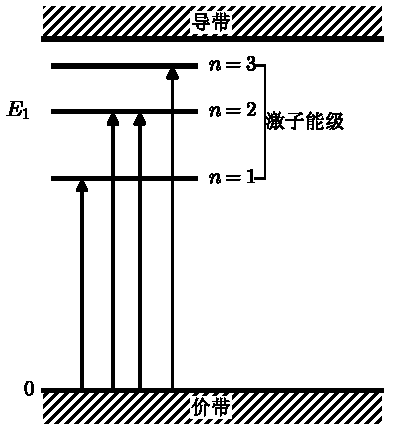
\includegraphics[width=6cm]{fig10-1.pdf}\\{\small 图 10.1\quad 激子能级}
\end{minipage}
\end{center}

以上结果说明：当入射光子能量小于禁带宽度时有一组激子吸收峰出现，吸收峰的位置可根据激子能级公式(10.2.9)确定.对于 $\mathrm{Cu}_{2}\mathrm{O}$ 晶体，其具体计算结果与格洛斯（Gross）等人\textsuperscript{[1]}在低温下测得吸收谱线一致.

式(10.2.9)左边第三项代表激子的平移动能，第二项是形成电子-空穴束缚对时所降低的能量
\begin{equation}
  E_{\mathrm{B}}(n)=-\frac{\overline{M}e^{4}}{2\hbar^{2}\epsilon^{2}n^{2}}
  \equiv\frac{-e^{2}}{2\epsilon n^{2}a_{\mathrm{ex}}}
\end{equation}
其中 $a_{\mathrm{ex}}$ 是基态 $\left(n=1, m=l=0\right)$ 的轨道半径，定义为激子半径.根据氢原子玻尔半径公式 $a_{\mathrm{H}}=\hbar^{2}/m_{\mathrm{e}}e^{2}$（$m_{\mathrm{e}}$ 是真空中电子质量），容易从式(10.2.10)求得激子半径
\begin{equation}
  a_{\mathrm{ex}}=\epsilon\,\frac{\hbar^{2}}{\overline{M}e^{2}}
  =\epsilon\biggl(\frac{m_{\mathrm{e}}}{\overline{M}}\biggr)a_{\mathrm{H}}
\end{equation}
对于瓦尼尔-莫特激子，由于 $a_{\mathrm{ex}}\gg a_{\mathrm{H}}$，必须要求晶体的介电常数 $\epsilon\gg1$，折合质量 $\overline{M}\leqslant m_{\mathrm{e}}$，才能形成大半径的激子.多数的半导体和绝缘晶体满足这一条件，因此瓦尼尔-莫特激子是常见的.根据式(10.2.11)，对于晶格常数较大、介电常数较小的晶体，其激子半径可能比晶格常数小，这时上述理论失效，我们必须考虑晶格的原子结构，从另一角度讨论问题.

\section{夫伦克耳激子}

夫伦克耳认为小激子运动问题实际上是同一原子内电子的激发态从一个原子向另一个原子的转移问题.

设晶体中有 $N$ 个原子，每个原子上有一个电子.原子中电子的基态为 $\phi_{\mathrm{s}}(\boldsymbol{r})$，其能量为 $\mathscr{E}_{\mathrm{s}}$，第一激发态为 $\phi_{\mathrm{p}}(\boldsymbol{r})$，能量是 $\mathscr{E}_{\mathrm{p}}$.因此，原子内电子从s态向p态的激发能为 $\mathscr{E}_{\mathrm{p}}-\mathscr{E}_{\mathrm{s}}$，$N$ 个电子系统的基态，应由 $\phi_{\mathrm{s}}(\boldsymbol{r}_{1}-\boldsymbol{R}_{1}),\cdots,\phi_{\mathrm{s}}(\boldsymbol{r}_{N}-\boldsymbol{R}_{N})$ 的斯莱特行列式组成.为讨论简单起见，在本节中暂时略去电子的自旋和不同格点 $(\boldsymbol{R}_{n}\neq\boldsymbol{R}_{m})$ 间原子波函数的重叠.这样，晶体的基态可写成
\begin{equation}
  \varPhi_{0}(\boldsymbol{r}_{1},\cdots,\boldsymbol{r}_{N})
  =\prod_{m}\phi_{\mathrm{s}}(\boldsymbol{r}_{m}-\boldsymbol{R}_{m})
\end{equation}
假定在第 $n$ 个原子内的电子从s态被激发到p态，则此局域激发态的波函数为
\begin{equation}
  \varPhi_{n}(\boldsymbol{r}_{1},\cdots,\boldsymbol{r}_{N})
  =\phi_{\mathrm{p}}(\boldsymbol{r}_{n}-\boldsymbol{R}_{n})
  \prod_{m(m\neq n)}\phi_{\mathrm{s}}(\boldsymbol{r}_{m}-\boldsymbol{R}_{m})
\end{equation}
$N$ 个原子系统的总哈密顿量由原子的哈密顿量 $h_{n}$ 和原子间互作用 $v_{nm}$ 组成
\begin{equation}
  H=\sum_{n}h_{n}+\sum_{n<m}\sum v_{nm}
\end{equation}
其中 $v_{nm}=e^{2}/|\boldsymbol{r}_{n}-\boldsymbol{r}_{m}|$ 是电子间库仑互作用.

产生如图10.2的局域激发能量为
\begin{equation}
  \mathscr{E}=\langle\varPhi_{n}|H|\varPhi_{n}\rangle
  -\langle\varPhi_{0}|H|\varPhi_{0}\rangle
\end{equation}

\begin{center}
\begin{minipage}{7.5cm}
\centering
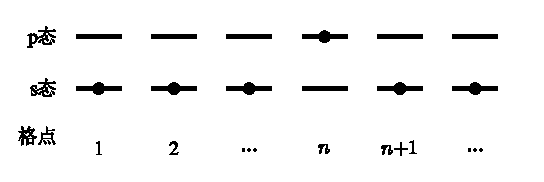
\includegraphics[width=7.5cm]{fig10-2.pdf}\\{\small 图 10.2\quad 局域激发态}
\end{minipage}
\end{center}

在平移对称系统中，此激发能与n无关，它近似等于原子中电子的激发能 $\mathscr{E}_{\mathrm{p}}-\mathscr{E}_{\mathrm{s}}$，说明局域激发可在任何格点产生.另一方面，H的非对角矩阵元为
\begin{equation}
\begin{aligned}
  H_{nm}&=\langle\varPhi_{n}|H|\varPhi_{m}\rangle\\
  &=\iint\mathrm{d}\boldsymbol{r}_{n}\mathrm{d}\boldsymbol{r}_{m}\,
  \phi_{\mathrm{p}}^{*}(\boldsymbol{r}_{n}-\boldsymbol{R}_{n})
  \phi_{\mathrm{s}}^{*}(\boldsymbol{r}_{m}-\boldsymbol{R}_{m})\\
  &\quad\times\frac{e^{2}}{|\boldsymbol{r}_{n}-\boldsymbol{r}_{m}|}
  \phi_{\mathrm{s}}(\boldsymbol{r}_{n}-\boldsymbol{R}_{n})
  \phi_{\mathrm{p}}(\boldsymbol{r}_{m}-\boldsymbol{R}_{m})
\end{aligned}
\end{equation}
{\emergencystretch=1em\relax
$H_{nm}$ 是“电荷分布”$-e\phi_{\mathrm{p}}^{*}(\boldsymbol{r}_{n}-\boldsymbol{R}_{n})\phi_{\mathrm{s}}(\boldsymbol{r}_{n}-\boldsymbol{R}_{n})$ 与 $-e\phi_{\mathrm{s}}^{*}(\boldsymbol{r}_{m}-\boldsymbol{R}_{m})\phi_{\mathrm{p}}(\boldsymbol{r}_{m}-\boldsymbol{R}_{m})$ 之间的库仑互作用，它使n格点原子上的电子激发转移到m格点原子上去，称为激发转移互作用.因此，哈密顿量H的单电子激发本征函数 $\varPsi$ 应当是在各格点上产生局域激发波函数 $\varPhi_{n}$ 的线性组合，与紧束缚近似的能带波函数相似，可将 $\varPsi$ 写为
\begin{equation}
  \varPsi_{\boldsymbol{K}}=\frac{1}{\sqrt{N}}\sum_{n}
  \mathrm{e}^{\mathrm{i}\boldsymbol{K}\cdot\boldsymbol{R}_{n}}\varPhi_{n}
\end{equation}
其中 $\boldsymbol{K}$ 为第一BZ中的波矢，这就是夫伦克耳激子的波函数.夫伦克耳激子的激发能应当由 $\langle\varPsi_{\boldsymbol{K}}|H|\varPsi_{\boldsymbol{K}}\rangle$ $-\langle\varPhi_{0}|H|\varPhi_{0}\rangle$ 决定：\par}
\begin{equation}
\begin{aligned}
  E_{\boldsymbol{K}}&\equiv\langle\varPsi_{\boldsymbol{K}}|H|\varPsi_{\boldsymbol{K}}\rangle
  -\langle\varPhi_{0}|H|\varPhi_{0}\rangle\\
  &=\mathscr{E}+\frac{1}{N}\sum_{m\neq n}\sum\,
  \langle\varPhi_{n}|H|\varPhi_{m}\rangle
  \mathrm{e}^{-\mathrm{i}\boldsymbol{K}\cdot(\boldsymbol{R}_{n}-\boldsymbol{R}_{m})}
\end{aligned}
\end{equation}

由式(10.3.5)可知，$H_{nm}$ 只是 $\boldsymbol{R}_{nm}=\boldsymbol{R}_{n}-\boldsymbol{R}_{m}$ 的函数，记为 $D(\boldsymbol{R}_{nm})$.因此，激子能级可表示为
\begin{equation}
  E_{\boldsymbol{K}}=\mathscr{E}
  +\sum_{\boldsymbol{R}_{nm}}^{\prime}D(\boldsymbol{R}_{nm})
  \mathrm{e}^{-\mathrm{i}\boldsymbol{K}\cdot\boldsymbol{R}_{nm}}
\end{equation}
式(10.3.8)代表夫伦克耳激子的能带公式，一般D很小，是窄带，惰性元素晶体具有这样的激子.例如在原子氪(Kr)组成的晶体中，观测到的激子吸收带很窄，分布在10.17 eV附近，与Kr原子中电子的跃迁能 $9.99$ eV［相当于 $(\mathscr{E}_{\mathrm{p}}-\mathscr{E}_{\mathrm{s}})$］相近，而Kr晶体的禁带宽度 $E_{\mathrm{g}}=11.7$ eV，说明激子能级分布在禁带中，并可用式(10.3.8)确定.

现在具体计算 $H_{nm}$ 的贡献，由式(10.3.5)作变数变换 $(\boldsymbol{r}_{n}-\boldsymbol{R}_{n})=\boldsymbol{r}$，$(\boldsymbol{r}_{m}-\boldsymbol{R}_{m})=\boldsymbol{r}^{\prime}$
\begin{equation}
\begin{aligned}
  H_{nm}&=\iint\mathrm{d}\boldsymbol{r}\mathrm{d}\boldsymbol{r}^{\prime}\,
  \phi_{\mathrm{p}}^{*}(\boldsymbol{r})\phi_{\mathrm{s}}^{*}(\boldsymbol{r}^{\prime})
  \frac{e^{2}}{|\boldsymbol{r}-\boldsymbol{r}^{\prime}-\boldsymbol{R}_{nm}|}
  \phi_{\mathrm{s}}(\boldsymbol{r})\phi_{\mathrm{p}}(\boldsymbol{r}^{\prime})\\
  &=D(\boldsymbol{R}_{nm})
\end{aligned}
\end{equation}
考虑到 $\phi_{\mathrm{s}}$ 和 $\phi_{\mathrm{p}}$ 的空间分布尺度小于原子间距，上式中 $\boldsymbol{\xi}=\boldsymbol{r}-\boldsymbol{r}^{\prime}$ 与 $\boldsymbol{R}_{nm}$ 相比是小量，可作展开：
\begin{equation}
  \frac{1}{|\boldsymbol{\xi}-\boldsymbol{R}_{nm}|}\approx\frac{1}{R_{nm}}
  \biggl[1+\frac{\boldsymbol{\xi}\cdot\boldsymbol{R}_{nm}}{R_{nm}^{2}}
  -\frac{\xi^{2}}{2R_{nm}^{2}}
  +\frac{3}{2}\frac{(\boldsymbol{\xi}\cdot\boldsymbol{R}_{nm})^{2}}{R_{nm}^{4}}
  +\cdots\biggr]
\end{equation}
将式(10.3.10)代入式(10.3.9)，求得
\begin{equation}
  H_{nm}=D(\boldsymbol{R}_{nm})\approx\frac{\mu^{2}}{R_{nm}^{3}}
  -\frac{3(\boldsymbol{\mu}\cdot\boldsymbol{R}_{nm})^{2}}{R_{nm}^{5}}
\end{equation}
其中
\begin{equation}
  \boldsymbol{\mu}\equiv\int\phi_{\mathrm{p}}^{*}(\boldsymbol{r})
  \left(-e\boldsymbol{r}\right)\phi_{\mathrm{s}}(\boldsymbol{r})\mathrm{d}\boldsymbol{r}
\end{equation}
代表偶极矩，式(10.3.11)正好是偶极-偶极相互作用.由此可计算激子能带公式中 $D(\boldsymbol{R}_{nm})$ 的傅里叶变换
\begin{equation}
  D_{\boldsymbol{K}}=\sum_{\boldsymbol{R}_{nm}}^{\prime}D(\boldsymbol{R}_{nm})
  \mathrm{e}^{-\mathrm{i}\boldsymbol{K}\cdot\boldsymbol{R}_{nm}}
\end{equation}
特别是 $D_{\boldsymbol{K}}$ 在 $\boldsymbol{K}=0$ 附近的数值.

设 $Kd\ll1$，这里 $d^{3}=\Omega$，Ω为元胞体积.以某一个原子为中心，作半径为 $R_{\mathrm{c}}$ 的球体，$R_{\mathrm{c}}$ 宏观小、微观大，并满足条件
\begin{equation}
  d\ll R_{\mathrm{c}}\ll K^{-1}
\end{equation}
则在 $R_{\mathrm{c}}$ 球外，求和式(10.3.13)可化为积分，而在 $R_{\mathrm{c}}$ 之内，则取 $\mathrm{e}^{-\mathrm{i}\boldsymbol{K}\cdot\boldsymbol{R}_{nm}}\approx1$.因此，有
\begin{equation}
  D_{\boldsymbol{K}}=\sum_{\boldsymbol{R}_{nm}<R_{\mathrm{c}}}D(\boldsymbol{R}_{nm})+I
\end{equation}
这里 I 是 $R_{\mathrm{c}}$ 球外的积分，求和化积分时利用
$\sum_{\boldsymbol{R}_{nm}}(\cdots)=(1/\Omega)\int(\cdots)\mathrm{d}\boldsymbol{R}$.根据图10.3，取 $\boldsymbol{K}$ 为z轴方向并设 $\theta_{0}$ 代表 $\boldsymbol{K}$ 与偶极矩 $\boldsymbol{\mu}$ 之间的夹角，$\theta$ 为 $\boldsymbol{K}$ 与 $\boldsymbol{R}$ 夹角，$\theta^{\prime}$ 为 $\boldsymbol{R}$ 与 $\boldsymbol{\mu}$ 的夹角，则I表示为积分：
\begin{equation}
\begin{aligned}
  I&=\Omega^{-1}\mu^{2}\int_{R_{\mathrm{c}}}^{\infty}\frac{\mathrm{d}R}{R}
  \int_{0}^{\pi}\mathrm{e}^{-\mathrm{i}KR\cos\theta}\sin\theta\,\mathrm{d}\theta
  \int_{-\pi}^{\pi}\left(1-3\cos^{2}\theta^{\prime}\right)\mathrm{d}\phi\\
  &=-\frac{4\pi}{3}\Omega^{-1}\mu^{2}\left(1-3\cos\theta_{0}^{2}\right)
  +O(K^{2}R_{\mathrm{c}}^{2})
  \qquad\left(Kd\ll1\right)
\end{aligned}
\end{equation}
最后求得，$Kd\ll1$ 时的 $D_{\boldsymbol{K}}$ 值为
\begin{equation}
  D_{\boldsymbol{K}}=\sum_{\boldsymbol{R}_{nm}<R_{\mathrm{c}}}D(\boldsymbol{R}_{nm})
  -\frac{4\pi}{3}\Omega^{-1}
  \Bigl[\mu^{2}-3\frac{(\boldsymbol{\mu}\cdot\boldsymbol{K})^{2}}{K^{2}}\Bigr]
\end{equation}
式(10.3.17)左边第二项在 $\boldsymbol{K}\parallel\boldsymbol{\mu}$ 时（纵向激子态）取 $\left(8\pi/3\right)\Omega^{-1}\mu^{2}$ 值，而 $\boldsymbol{K}\perp\boldsymbol{\mu}$ 时（横向激子态）取 $-\left(4\pi/3\right)\Omega^{-1}\mu^{2}$，两者之差为 $4\pi\Omega^{-1}\mu^{2}$，它代表 $\boldsymbol{K}\to0$ 时纵向和横向激子状态的能级差.纵向和横向激子态间的能级分裂是激子问题中的普遍现象，并非夫伦克耳激子的独特属性.

\begin{center}
\begin{minipage}{5.5cm}
\centering
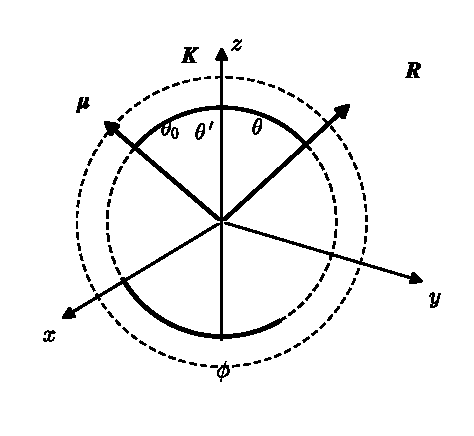
\includegraphics[width=5.5cm]{fig10-3.pdf}\\{\small 图 10.3\quad 积分 I 的计算图}
\end{minipage}
\end{center}

\section{\texorpdfstring{电子-空穴互作用的多体理论\textsuperscript{[2]}}{电子-空穴互作用的多体理论[2]}}

本节用二次量子化方法处理电子-空穴互作用问题，并将在 $a_{\mathrm{ex}}\gg d$ 和 $a_{\mathrm{ex}}\ll d$ 两种极限情况下分别求瓦尼尔-莫特激子和夫伦克耳激子的方程.

设单电子哈密顿量为 $h(\boldsymbol{p},\boldsymbol{r})$，它包括电子的动能和晶格周期场的位能，电子间互作用势能为
\begin{equation}
  v(\boldsymbol{r}-\boldsymbol{r}^{\prime})
  =\frac{e^{2}}{|\boldsymbol{r}-\boldsymbol{r}^{\prime}|}
\end{equation}
多电子系统的哈密顿量在二次量子化表象中写为
\begin{equation}
\begin{aligned}
  H&=\int\mathrm{d}\boldsymbol{r}\,\varPsi^{+}(\boldsymbol{r})h(\boldsymbol{p},\boldsymbol{r})\varPsi(\boldsymbol{r})\\
  &\quad+\frac{1}{2}\iint\mathrm{d}\boldsymbol{r}\mathrm{d}\boldsymbol{r}^{\prime}\,
  \varPsi^{+}(\boldsymbol{r})\varPsi^{+}(\boldsymbol{r}^{\prime})
  v(\boldsymbol{r}-\boldsymbol{r}^{\prime})
  \varPsi(\boldsymbol{r}^{\prime})\varPsi(\boldsymbol{r})
\end{aligned}
\end{equation}
态矢量 $\varPsi(\boldsymbol{r})$ 可分别利用布洛赫函数 $\phi_{\nu\boldsymbol{k}}(\boldsymbol{r})$ 及瓦尼尔函数 $a_{\nu}(\boldsymbol{r}-\boldsymbol{R}_{n})$ 作基函数表示成
\begin{equation}
\begin{aligned}
  \varPsi(\boldsymbol{r})&=\sum_{\nu,\boldsymbol{k}}C_{\nu\boldsymbol{k}}\phi_{\nu\boldsymbol{k}}(\boldsymbol{r})\\
  &=\sum_{\nu,n}C_{\nu n}a_{\nu}(\boldsymbol{r}-\boldsymbol{R}_{n})
\end{aligned}
\end{equation}
$C_{\nu\boldsymbol{k}}$，$C_{\nu\boldsymbol{k}}^{+}$ 代表ν能带中 $\boldsymbol{k}$ 波矢电子的消灭与产生算符，而 $C_{\nu n}$ 和 $C_{\nu n}^{+}$ 则是局域表示中消灭及产生算符，n是格点指标.

利用布洛赫函数与瓦尼尔函数间关系
\begin{equation}
  a_{\nu}(\boldsymbol{r}-\boldsymbol{R}_{n})=(1/\sqrt{N})\sum_{\boldsymbol{k}}
  \mathrm{e}^{-\mathrm{i}\boldsymbol{k}\cdot\boldsymbol{R}_{n}}\phi_{\nu\boldsymbol{k}}(\boldsymbol{r})
\end{equation}
可求得两组算子间关系为
\begin{equation}
  C_{\nu\boldsymbol{k}}=\frac{1}{\sqrt{N}}\sum_{n}
  \mathrm{e}^{-\mathrm{i}\boldsymbol{k}\cdot\boldsymbol{R}_{n}}C_{\nu n}
\end{equation}
算子满足费密子对易律
\begin{equation}
  \bigl[C_{\nu\boldsymbol{k}},C_{\mu\boldsymbol{k}^{\prime}}^{+}\bigr]_{+}
  =\delta_{\nu\mu}\delta_{\boldsymbol{k}\boldsymbol{k}^{\prime}};
  \quad
  \bigl[C_{\nu\boldsymbol{k}},C_{\mu\boldsymbol{k}^{\prime}}\bigr]_{+}
  =\bigl[C_{\nu\boldsymbol{k}}^{+},C_{\mu\boldsymbol{k}^{\prime}}^{+}\bigr]_{+}=0
\end{equation}
\begin{equation}
  \bigl[C_{\nu n},C_{\mu m}^{+}\bigr]_{+}
  =\delta_{\nu\mu}\delta_{nm};
  \quad
  \bigl[C_{\nu n},C_{\mu m}\bigr]_{+}
  =\bigl[C_{\nu n}^{+},C_{\mu m}^{+}\bigr]_{+}=0
\end{equation}
设 $\mu$ 代表绝缘晶体中的满带（价带）指标，ν代表空带（导带）指标，则在单电子近似范围内系统的基态为
\begin{equation}
  |g\rangle=\prod_{\mu^{\prime}\boldsymbol{k}}C_{\mu^{\prime}\boldsymbol{k}}^{+}|0\rangle
\end{equation}
这时 $|0\rangle$ 是真空态，$\mu^{\prime}$ 取所有满带的值.

现在考虑有一个电子从满带的 $(\mu,\boldsymbol{k}^{\prime})$ 态被激发至导带 $(\nu,\boldsymbol{k})$ 态上，形成了 $C_{\nu\boldsymbol{k}}^{+}C_{\mu\boldsymbol{k}^{\prime}}|g\rangle$ 的激发态，这个激发态的总波矢为
\begin{equation}
  \boldsymbol{K}=\boldsymbol{k}-\boldsymbol{k}^{\prime}
\end{equation}
因为在满带 $\mu$ 中失去 $\boldsymbol{k}^{\prime}$ 电子后产生了空穴，其波矢为 $-\boldsymbol{k}^{\prime}$.由于哈密顿量H具有平移对称性，因此总波矢 $\boldsymbol{K}$ 应为量子数，而H的单粒子激发本征函数 $|e\rangle$ 由 $\boldsymbol{K}$ 一定时所有可能的 $(\boldsymbol{k},\boldsymbol{k}^{\prime})$ 激发的线性组合构成
\begin{equation}
  |e\rangle=\sum_{\boldsymbol{k}}f(\boldsymbol{k})
  C_{\nu\boldsymbol{k}}^{+}C_{\mu,\boldsymbol{k}-\boldsymbol{K}}|g\rangle
  \equiv B^{+}|g\rangle
\end{equation}
或利用瓦尼尔表象将上式改写为
\begin{equation}
  |e\rangle=\frac{1}{\sqrt{N}}\sum_{m,l}
  \mathrm{e}^{\mathrm{i}\boldsymbol{K}\cdot\boldsymbol{R}_{m}}F(\boldsymbol{R}_{l})
  C_{\nu,m+l}^{+}C_{\mu m}|g\rangle\equiv B^{+}|g\rangle
\end{equation}
其中
\begin{equation}
\left.
\begin{aligned}
  F(\boldsymbol{R}_{l})&=\frac{1}{\sqrt{N}}\sum_{\boldsymbol{k}}f(\boldsymbol{k})
  \mathrm{e}^{\mathrm{i}\boldsymbol{k}\cdot\boldsymbol{R}_{l}}\\
  f(\boldsymbol{k})&=\frac{1}{\sqrt{N}}\sum_{l}F(\boldsymbol{R}_{l})
  \mathrm{e}^{-\mathrm{i}\boldsymbol{k}\cdot\boldsymbol{R}_{l}}
\end{aligned}\right\}
\end{equation}
$f$ 与 $F$ 的归一条件为
\begin{equation}
  \sum_{\boldsymbol{k}}|f(\boldsymbol{k})|^{2}
  =\sum_{l}|F(\boldsymbol{R}_{l})|^{2}=1
\end{equation}
为简单起见，在导出式(10.4.11)时，我们只限于考虑系统中激发了电子和空穴的价带 $\mu$ 和导带ν，而略去其它能带的影响.

式(10.4.10)和(10.4.11)中 $f(\boldsymbol{k})$ 及 $F(\boldsymbol{R}_{l})$ 是二体运动的概率振幅.例如，$F(\boldsymbol{R}_{l})$ 代表导带ν中有一个电子，价带 $\mu$ 中有一个空穴的相对波函数，$\boldsymbol{R}_{l}$ 是电子-空穴的相对坐标，$\boldsymbol{K}$ 代表电子-空穴对平移运动的波矢，如果能求得 $F(\boldsymbol{R}_{l})$ 或 $f(\boldsymbol{k})$ 所满足的运动方程，那么N粒子问题就简化为二体问题了.下面，我们首先给出哈特利-福克近似下的二体运动方程，然后分别讨论大激子与小激子的极限情况.

\subsection*{1. $f(\boldsymbol{k})$和$F(\boldsymbol{R}_{l})$的运动方程}

我们的目的是求激发态 $|e\rangle$ 和激发能
\begin{equation}
  E=E_{e}-E_{0}
\end{equation}
其中 $E_{0}$ 是基态 $|g\rangle$ 的能量，$E_{e}$ 是激发态 $|e\rangle$ 的能量，它们分别满足本征方程
\begin{equation}
  0=\left(H-E_{0}\right)|g\rangle
\end{equation}
和
\begin{equation}
  0=\left(H-E_{e}\right)|e\rangle
\end{equation}
利用式(10.4.10)引入算符 $B^{+}$，可将 $|e\rangle$ 的本征方程改写为
\begin{equation}
\begin{aligned}
  0&=\left(H-E_{e}\right)|e\rangle\\
  &=\left(HB^{+}-E_{e}B^{+}\right)|g\rangle\\
  &=\left(\left[H,B^{+}\right]+B^{+}H-E_{e}B^{+}\right)|g\rangle
\end{aligned}
\end{equation}
利用式(10.4.14)和(10.4.15)，得到算符 $B^{+}$ 的方程
\begin{equation}
  \left[H,B^{+}\right]|g\rangle=EB^{+}|g\rangle
\end{equation}
E 为激发能.将式(10.4.10)所给出的 $B^{+}$ 代入上式，并左乘 $\langle g|C_{\mu\boldsymbol{k}^{\prime}-\boldsymbol{K}}^{+}C_{\nu\boldsymbol{k}^{\prime}}$ 可求得 $f(\boldsymbol{k})$ 的运动方程
\begin{equation}
  \sum_{\boldsymbol{k}}H_{\boldsymbol{k}^{\prime}\boldsymbol{k}}f(\boldsymbol{k})
  =Ef(\boldsymbol{k}^{\prime})
\end{equation}
这里有效哈密顿量 $H_{\boldsymbol{k}^{\prime}\boldsymbol{k}}$ 定义为
\begin{equation}
  H_{\boldsymbol{k}^{\prime}\boldsymbol{k}}\equiv\langle g|
  C_{\mu,\boldsymbol{k}^{\prime}-\boldsymbol{K}}^{+}C_{\nu\boldsymbol{k}^{\prime}}
  \left[H,C_{\nu\boldsymbol{k}}^{+}C_{\mu,\boldsymbol{k}-\boldsymbol{K}}\right]|g\rangle
\end{equation}
利用对易关系式(10.4.6)，经直接计算可以求得哈特利-福克近似的结果为
\begin{equation}
\begin{aligned}
  H_{\boldsymbol{k}^{\prime}\boldsymbol{k}}
  &=\delta_{\boldsymbol{k}^{\prime}\boldsymbol{k}}\{\mathscr{E}_{\nu}(\boldsymbol{k})
  -\mathscr{E}_{\mu}(\boldsymbol{k}-\boldsymbol{K})\}\\
  &\quad-\langle\nu,\boldsymbol{k}^{\prime};\mu,(\boldsymbol{k}-\boldsymbol{K})|v|
  \nu,\boldsymbol{k};\mu,(\boldsymbol{k}^{\prime}-\boldsymbol{K})\rangle\\
  &\quad+\langle\nu,\boldsymbol{k}^{\prime};\mu,(\boldsymbol{k}-\boldsymbol{K})|v|
  \mu,(\boldsymbol{k}^{\prime}-\boldsymbol{K});\nu,k\rangle
\end{aligned}
\end{equation}
这里
\begin{equation}
\begin{aligned}
  &\langle\lambda_{1},\boldsymbol{k}_{1};\lambda_{2},\boldsymbol{k}_{2}|v|
  \lambda_{3},\boldsymbol{k}_{3};\lambda_{4},\boldsymbol{k}_{4}\rangle\\
  &\equiv\iint\mathrm{d}\boldsymbol{r}\mathrm{d}\boldsymbol{r}^{\prime}\,
  \phi_{\lambda_{1}\boldsymbol{k}_{1}}^{*}(\boldsymbol{r})
  \phi_{\lambda_{2}\boldsymbol{k}_{2}}^{*}(\boldsymbol{r}^{\prime})
  v(\boldsymbol{r}-\boldsymbol{r}^{\prime})
  \phi_{\lambda_{3}\boldsymbol{k}_{3}}(\boldsymbol{r})
  \phi_{\lambda_{4}\boldsymbol{k}_{4}}(\boldsymbol{r}^{\prime})
\end{aligned}
\end{equation}
显然，式(10.4.21)右边第三项代表库仑势作用，第四项为交换作用.应当注意到式(10.4.21)中第三、四项与电子-电子互作用情况相差负号，这是由于激子问题涉及电子与空穴相互作用，而空穴带正电的缘故.$\mathscr{E}_{\nu}(\boldsymbol{k})$ 和 $\mathscr{E}_{\mu}(\boldsymbol{k}-\boldsymbol{K})$ 为导带及满带中电子在哈特利-福克近似下的能量，它满足HF方程
\begin{equation}
\begin{aligned}
  &h(\boldsymbol{p},\boldsymbol{r})\phi_{\lambda\boldsymbol{k}}(\boldsymbol{r})
  +\sum_{\mu^{\prime},\boldsymbol{k}^{\prime}}\int\mathrm{d}\boldsymbol{r}^{\prime}\,
  v(\boldsymbol{r}-\boldsymbol{r}^{\prime})\phi_{\mu^{\prime}\boldsymbol{k}^{\prime}}(\boldsymbol{r}^{\prime})
  \times\\
  &\qquad\left[\phi_{\mu^{\prime}\boldsymbol{k}^{\prime}}(\boldsymbol{r}^{\prime})\phi_{\lambda\boldsymbol{k}}(\boldsymbol{r})
  -\phi_{\mu^{\prime}\boldsymbol{k}^{\prime}}(\boldsymbol{r})\phi_{\lambda\boldsymbol{k}}(\boldsymbol{r}^{\prime})\right]\\
  &\qquad=\mathscr{E}_{\lambda}(\boldsymbol{k})\phi_{\lambda\boldsymbol{k}}(\boldsymbol{r})
\end{aligned}
\end{equation}
利用式(10.4.12)将 $\boldsymbol{k}$ 表象中 $f(\boldsymbol{k})$ 的运动方程(10.4.19)变换到 $\boldsymbol{R}$ 表象，从而求得 $F(\boldsymbol{R})$ 的运动方程
\begin{equation}
  \sum_{l^{\prime}}H_{l^{\prime}l}F(\boldsymbol{R}_{l^{\prime}})=EF(\boldsymbol{R}_{l})
\end{equation}
这里
\begin{equation}
  H_{l^{\prime}l}=\frac{1}{N}\sum_{\boldsymbol{k},\boldsymbol{k}^{\prime}}
  \mathrm{e}^{\mathrm{i}\boldsymbol{k}^{\prime}\cdot\boldsymbol{R}_{l}}H_{\boldsymbol{k}^{\prime}\boldsymbol{k}}
  \mathrm{e}^{-\mathrm{i}\boldsymbol{k}\cdot\boldsymbol{R}_{l^{\prime}}}
\end{equation}
其中 $\boldsymbol{R}_{l}$ 是电子-空穴的相对坐标.将式(10.4.21)代入式(10.4.25)
\begin{equation}
\begin{aligned}
  H_{l^{\prime}l}&=\frac{1}{N}\sum_{\boldsymbol{k}^{\prime}}
  \mathscr{E}_{\nu}(\boldsymbol{k}^{\prime})
  \mathrm{e}^{\mathrm{i}\boldsymbol{k}^{\prime}\cdot(\boldsymbol{R}_{l}-\boldsymbol{R}_{l^{\prime}})}
  -\frac{1}{N}\sum_{\boldsymbol{k}}\mathscr{E}_{\mu}(\boldsymbol{k}-\boldsymbol{K})
  \mathrm{e}^{\mathrm{i}\boldsymbol{k}\cdot(\boldsymbol{R}_{l}-\boldsymbol{R}_{l^{\prime}})}\\
  &\quad-\frac{1}{N}\sum_{\boldsymbol{k},\boldsymbol{k}^{\prime}}
  \mathrm{e}^{\mathrm{i}\boldsymbol{k}^{\prime}\cdot\boldsymbol{R}_{l}}
  \langle\mathrm{I}\rangle
  \mathrm{e}^{-\mathrm{i}\boldsymbol{k}\cdot\boldsymbol{R}_{l^{\prime}}}
  +\frac{1}{N}\sum_{\boldsymbol{k},\boldsymbol{k}^{\prime}}
  \mathrm{e}^{\mathrm{i}\boldsymbol{k}^{\prime}\cdot\boldsymbol{R}_{l^{\prime}}}
  \langle\mathrm{II}\rangle
  \mathrm{e}^{-\mathrm{i}\boldsymbol{k}\cdot\boldsymbol{R}_{l^{\prime}}}
\end{aligned}
\end{equation}
这里 $\langle\mathrm{I}\rangle$ 代表式(10.4.21)中库仑项，$\langle\mathrm{II}\rangle$ 是交换作用项.
\begin{equation}
\begin{aligned}
  \langle\mathrm{I}\rangle&\equiv\langle\nu,\boldsymbol{k}^{\prime};
  \mu,(\boldsymbol{k}-\boldsymbol{K})|v|\nu,\boldsymbol{k};
  \mu,(\boldsymbol{k}^{\prime}-\boldsymbol{K})\rangle\\
  &=\iint\mathrm{d}\boldsymbol{r}\mathrm{d}\boldsymbol{r}^{\prime}\,
  \phi_{\nu\boldsymbol{k}^{\prime}}^{*}(\boldsymbol{r})
  \phi_{\mu(\boldsymbol{k}-\boldsymbol{K})}^{*}(\boldsymbol{r}^{\prime})
  v(\boldsymbol{r}-\boldsymbol{r}^{\prime})
  \phi_{\nu\boldsymbol{k}}(\boldsymbol{r})
  \phi_{\mu(\boldsymbol{k}^{\prime}-\boldsymbol{K})}(\boldsymbol{r}^{\prime})\\
  &=\frac{1}{N^{2}}\sum_{\boldsymbol{R}_{1}\cdots\boldsymbol{R}_{4}}
  \exp\bigl\{-\mathrm{i}[\boldsymbol{k}^{\prime}\cdot\boldsymbol{R}_{1}
  +(\boldsymbol{k}-\boldsymbol{K})\cdot\boldsymbol{R}_{2}
  -\boldsymbol{k}\cdot\boldsymbol{R}_{3}
  -(\boldsymbol{k}^{\prime}-\boldsymbol{K})\cdot\boldsymbol{R}_{4}]\bigr\}\\
  &\qquad\times\iint\mathrm{d}\boldsymbol{r}\mathrm{d}\boldsymbol{r}^{\prime}\,
  \boldsymbol{a}_{\nu}^{*}(\boldsymbol{r}-\boldsymbol{R}_{1})
  \boldsymbol{a}_{\mu}^{*}(\boldsymbol{r}^{\prime}-\boldsymbol{R}_{2})
  v(\boldsymbol{r}-\boldsymbol{r}^{\prime})
  \boldsymbol{a}_{\nu}(\boldsymbol{r}-\boldsymbol{R}_{3})
  \boldsymbol{a}_{\mu}(\boldsymbol{r}^{\prime}-\boldsymbol{R}_{4})\\
  &\approx\frac{1}{N^{2}}\sum_{\boldsymbol{R}_{1},\boldsymbol{R}_{2}}
  \exp\bigl\{-\mathrm{i}(\boldsymbol{k}^{\prime}-\boldsymbol{k})
  \cdot(\boldsymbol{R}_{1}-\boldsymbol{R}_{2})\bigr\}\\
  &\qquad\times\iint\mathrm{d}\boldsymbol{r}\mathrm{d}\boldsymbol{r}^{\prime}\,
  \boldsymbol{a}_{\nu}^{*}(\boldsymbol{r}-\boldsymbol{R}_{1})
  \boldsymbol{a}_{\mu}^{*}(\boldsymbol{r}^{\prime}-\boldsymbol{R}_{2})
  v(\boldsymbol{r}-\boldsymbol{r}^{\prime})
  \boldsymbol{a}_{\nu}(\boldsymbol{r}-\boldsymbol{R}_{1})
  \boldsymbol{a}_{\mu}(\boldsymbol{r}^{\prime}-\boldsymbol{R}_{2})\\
  &\equiv\frac{1}{N}\sum_{\boldsymbol{R}_{12}}
  \mathrm{e}^{-\mathrm{i}(\boldsymbol{k}^{\prime}-\boldsymbol{k})\cdot\boldsymbol{R}_{12}}
  V(\boldsymbol{R}_{12})
  \qquad(\boldsymbol{R}_{12}=\boldsymbol{R}_{1}-\boldsymbol{R}_{2})
\end{aligned}
\end{equation}
上式中利用了瓦尼尔函数 $\boldsymbol{a}_{\lambda}(\boldsymbol{r}-\boldsymbol{R}_{n})$ 的局域特性，认为瓦尼尔函数与原子轨道函数相似，是局限于 $\boldsymbol{R}_{n}$ 格点周围的函数.这时可近似取 $\boldsymbol{R}_{1}=\boldsymbol{R}_{3}$ 和 $\boldsymbol{R}_{2}=\boldsymbol{R}_{4}$，并得到式(10.4.27)的第四个等式.

类似的，用瓦尼尔函数表示 $\langle\mathrm{II}\rangle$，可求得如下结果：
\begin{equation}
\begin{aligned}
  \langle\mathrm{II}\rangle&\equiv\langle\nu,\boldsymbol{k}^{\prime};
  \mu,(\boldsymbol{k}-\boldsymbol{K})|v|\mu,(\boldsymbol{k}^{\prime}-\boldsymbol{K});
  \nu,k\rangle\\
  &=\frac{1}{N^{2}}\sum_{\boldsymbol{R}_{1}\cdots\boldsymbol{R}_{4}}
  \exp\bigl\{-\mathrm{i}[\boldsymbol{k}^{\prime}\cdot\boldsymbol{R}_{1}
  +(\boldsymbol{k}-\boldsymbol{K})\cdot\boldsymbol{R}_{2}\\
  &\qquad-(\boldsymbol{k}^{\prime}-\boldsymbol{K})\cdot\boldsymbol{R}_{3}
  -\boldsymbol{k}\cdot\boldsymbol{R}_{4}]\bigr\}
  \times\iint\mathrm{d}\boldsymbol{r}\mathrm{d}\boldsymbol{r}^{\prime}\,
  \boldsymbol{a}_{\nu}^{*}(\boldsymbol{r}-\boldsymbol{R}_{1})
  \boldsymbol{a}_{\mu}^{*}(\boldsymbol{r}^{\prime}-\boldsymbol{R}_{2})\\
  &\qquad\times v(\boldsymbol{r}-\boldsymbol{r}^{\prime})
  \boldsymbol{a}_{\mu}(\boldsymbol{r}-\boldsymbol{R}_{3})
  \boldsymbol{a}_{\nu}(\boldsymbol{r}^{\prime}-\boldsymbol{R}_{4})\\
  &\approx\frac{1}{N^{2}}\sum_{\boldsymbol{R}_{1},\boldsymbol{R}_{2}}
  \exp\bigl\{-\mathrm{i}\boldsymbol{K}\cdot(\boldsymbol{R}_{1}-\boldsymbol{R}_{2})\bigr\}\\
  &\qquad\times\iint\mathrm{d}\boldsymbol{r}\mathrm{d}\boldsymbol{r}^{\prime}\,
  \boldsymbol{a}_{\nu}^{*}(\boldsymbol{r}-\boldsymbol{R}_{1})
  \boldsymbol{a}_{\mu}^{*}(\boldsymbol{r}^{\prime}-\boldsymbol{R}_{2})
  v(\boldsymbol{r}-\boldsymbol{r}^{\prime})
  \boldsymbol{a}_{\mu}(\boldsymbol{r}-\boldsymbol{R}_{1})
  \boldsymbol{a}_{\nu}(\boldsymbol{r}^{\prime}-\boldsymbol{R}_{2})\\
  &\equiv\frac{1}{N}\sum_{\boldsymbol{R}_{12}}
  \mathrm{e}^{-\mathrm{i}\boldsymbol{K}\cdot\boldsymbol{R}_{12}}W(\boldsymbol{R}_{12})
\end{aligned}
\end{equation}
这样，式(10.4.26)右边第三、四项为
\begin{equation}
\left.
\begin{aligned}
  \frac{1}{N}\sum_{\boldsymbol{k},\boldsymbol{k}^{\prime}}
  \mathrm{e}^{\mathrm{i}\boldsymbol{k}^{\prime}\cdot\boldsymbol{R}_{l}}
  \langle\mathrm{I}\rangle
  \mathrm{e}^{-\mathrm{i}\boldsymbol{k}\cdot\boldsymbol{R}_{l^{\prime}}}
  &=\delta_{ll^{\prime}}V(\boldsymbol{R}_{l})\\
  \frac{1}{N}\sum_{\boldsymbol{k},\boldsymbol{k}^{\prime}}
  \mathrm{e}^{\mathrm{i}\boldsymbol{k}^{\prime}\cdot\boldsymbol{R}_{l}}
  \langle\mathrm{II}\rangle
  \mathrm{e}^{-\mathrm{i}\boldsymbol{k}\cdot\boldsymbol{R}_{l^{\prime}}}
  &=\delta_{l0}\delta_{l^{\prime}0}W_{\boldsymbol{K}}
\end{aligned}\right\}
\end{equation}
其中
\begin{equation*}
  W_{\boldsymbol{K}}=\sum_{m}\mathrm{e}^{-\mathrm{i}\boldsymbol{K}\cdot\boldsymbol{R}_{m}}W(\boldsymbol{R}_{m})
\end{equation*}
根据式(10.4.27)与(10.4.28)，$V(\boldsymbol{R}_{l})$ 和 $W(\boldsymbol{R}_{m})$ 定义为
\begin{equation}
  V(\boldsymbol{R}_{l})\equiv\iint\mathrm{d}\boldsymbol{r}\mathrm{d}\boldsymbol{r}^{\prime}\,
  \boldsymbol{a}_{\nu}^{*}(\boldsymbol{r}-\boldsymbol{R}_{l})
  \boldsymbol{a}_{\mu}^{*}(\boldsymbol{r}^{\prime})
  v(\boldsymbol{r}-\boldsymbol{r}^{\prime})
  \boldsymbol{a}_{\nu}(\boldsymbol{r}-\boldsymbol{R}_{l})
  \boldsymbol{a}_{\mu}(\boldsymbol{r}^{\prime})
\end{equation}
\begin{equation}
  W(\boldsymbol{R}_{m})\equiv\int\mathrm{d}\boldsymbol{r}\mathrm{d}\boldsymbol{r}^{\prime}\,
  \boldsymbol{a}_{\nu}^{*}(\boldsymbol{r}-\boldsymbol{R}_{m})
  \boldsymbol{a}_{\mu}^{*}(\boldsymbol{r}^{\prime})
  v(\boldsymbol{r}-\boldsymbol{r}^{\prime})
  \boldsymbol{a}_{\mu}(\boldsymbol{r}-\boldsymbol{R}_{m})
  \boldsymbol{a}_{\nu}(\boldsymbol{r}^{\prime})
\end{equation}
式(10.4.26)右边第一项可定义为 $E_{\nu}(\boldsymbol{R}_{l}-\boldsymbol{R}_{l^{\prime}})$
\begin{equation}
  E_{\nu}(\boldsymbol{R}_{l}-\boldsymbol{R}_{l^{\prime}})\equiv\frac{1}{N}
  \sum_{\boldsymbol{k}}\mathscr{E}_{\nu}(\boldsymbol{k})
  \mathrm{e}^{\mathrm{i}\boldsymbol{k}\cdot(\boldsymbol{R}_{l}-\boldsymbol{R}_{l^{\prime}})}
\end{equation}
其逆变换是
\begin{equation}
  \mathscr{E}_{\nu}(\boldsymbol{k})=\sum_{m}E_{\nu}(\boldsymbol{R}_{m})
  \mathrm{e}^{-\mathrm{i}\boldsymbol{k}\cdot\boldsymbol{R}_{m}}
\end{equation}
由于 $E_{\nu}(\boldsymbol{R}_{l}-\boldsymbol{R}_{l^{\prime}})$ 项在方程式(10.4.24)中是作用于函数F上的，我们可以利用第八章§8讨论有效哈密顿量时的技巧作下列简化：
\begin{equation}
\begin{aligned}
  \sum_{l^{\prime}}E_{\nu}(\boldsymbol{R}_{l}-\boldsymbol{R}_{l^{\prime}})F(\boldsymbol{R}_{l^{\prime}})
  &=\sum_{m}E_{\nu}(\boldsymbol{R}_{m})F(\boldsymbol{R}_{l}-\boldsymbol{R}_{m})\\
  &=\sum_{m}E_{\nu}(\boldsymbol{R}_{m})\sum_{p=0}^{\infty}\frac{1}{p!}
  (-\boldsymbol{R}_{m}\cdot\nabla_{l})^{p}F(\boldsymbol{R}_{l})\\
  &=\sum_{m}E_{\nu}(\boldsymbol{R}_{m})
  \exp[-\boldsymbol{R}_{m}\cdot\nabla_{l}]F(\boldsymbol{R}_{l})\\
  &=\mathscr{E}_{\nu}(-\mathrm{i}\nabla_{l})F(\boldsymbol{R}_{l})\\
  &=\sum_{l^{\prime}}\mathscr{E}_{\nu}(-\mathrm{i}\nabla_{l})\delta_{ll^{\prime}}F(\boldsymbol{R}_{l^{\prime}})
\end{aligned}
\end{equation}
这时式(10.4.26)右边第二项可写成
\begin{equation}
\begin{aligned}
  \frac{1}{N}\sum_{\boldsymbol{k}}\mathscr{E}_{\mu}(\boldsymbol{k}-\boldsymbol{K})
  \mathrm{e}^{\mathrm{i}\boldsymbol{k}\cdot(\boldsymbol{R}_{l}-\boldsymbol{R}_{l^{\prime}})}
  &=\mathrm{e}^{\mathrm{i}\boldsymbol{K}\cdot(\boldsymbol{R}_{l}-\boldsymbol{R}_{l^{\prime}})}
  \frac{1}{N}\sum_{\boldsymbol{k}}\mathscr{E}_{\mu}(\boldsymbol{k})
  \mathrm{e}^{\mathrm{i}\boldsymbol{k}\cdot(\boldsymbol{R}_{l}-\boldsymbol{R}_{l^{\prime}})}\\
  &=\mathrm{e}^{\mathrm{i}\boldsymbol{K}\cdot(\boldsymbol{R}_{l}-\boldsymbol{R}_{l^{\prime}})}
  E(\boldsymbol{R}_{l}-\boldsymbol{R}_{l^{\prime}})
\end{aligned}
\end{equation}
类似于式(10.4.34)的作法，求得这一项在F方程(10.4.24)中的贡献为
\begin{equation}
\begin{aligned}
  &\sum_{l^{\prime}}\mathrm{e}^{\mathrm{i}\boldsymbol{K}\cdot(\boldsymbol{R}_{l}-\boldsymbol{R}_{l^{\prime}})}
  E_{\mu}(\boldsymbol{R}_{l}-\boldsymbol{R}_{l^{\prime}})F(\boldsymbol{R}_{l^{\prime}})\\
  &\quad=\sum_{m}\mathrm{e}^{\mathrm{i}\boldsymbol{K}\cdot\boldsymbol{R}_{m}}
  E_{\mu}(\boldsymbol{R}_{m})F(\boldsymbol{R}_{l}-\boldsymbol{R}_{m})\\
  &\quad=\sum_{m}E_{\mu}(\boldsymbol{R}_{m})
  \exp[\boldsymbol{R}_{m}\cdot(-\nabla_{l}+\mathrm{i}\boldsymbol{K})]F(\boldsymbol{R}_{l})\\
  &\quad=\mathscr{E}_{\mu}(-\mathrm{i}\nabla_{l}-\boldsymbol{K})F(\boldsymbol{R}_{l})\\
  &\quad=\sum_{l^{\prime}}\mathscr{E}_{\mu}(-\mathrm{i}\nabla_{l}-\boldsymbol{K})\delta_{ll^{\prime}}F(\boldsymbol{R}_{l^{\prime}})
\end{aligned}
\end{equation}
根据式(10.4.26)和(10.4.29)—(10.4.36)，可将电子-空穴对激发的有效哈密顿量，写成下列简单形式：
\begin{equation}
  H_{ll^{\prime}}=\{\mathscr{E}_{\nu}(-\mathrm{i}\nabla_{l})
  -\mathscr{E}_{\mu}(-\mathrm{i}\nabla_{l}-\boldsymbol{K})-V(\boldsymbol{R}_{l})\}\delta_{ll^{\prime}}
  +\delta_{l0}\delta_{l^{\prime}0}W_{\boldsymbol{K}}
\end{equation}
将上式代入F的运动方程(10.4.24)，可统一处理大激子与小激子问题.我们将证明：在激子半径比晶格常数大的极限情况下，可导出瓦尼尔-莫特激子方程(10.2.5).在相反极限下，则求出夫伦克耳激子的能带公式(10.3.8).

\subsection*{2. 瓦尼尔-莫特激子}

当价带 $\mu$ 中空穴与导带ν中电子的相对距离 $\boldsymbol{R}$ 比较大时，可以忽略 $H_{ll^{\prime}}$ 中交换项 $W_{\boldsymbol{K}}$ 的贡献，因为它是短程作用.$H_{ll^{\prime}}$ 中重要的是库仑项 $V(\boldsymbol{R})$，它是长程作用.根据式(10.4.30)，考虑到瓦尼尔函数 $|\boldsymbol{a}_{\nu}(\boldsymbol{r}-\boldsymbol{R})|^{2}$ 是集中分布在 $\boldsymbol{R}$ 附近的局域函数，可将库仑项写成下列近似式：
\begin{equation}
\begin{aligned}
  V(\boldsymbol{R})&=\iint\mathrm{d}\boldsymbol{r}\mathrm{d}\boldsymbol{r}^{\prime}\,
  |\boldsymbol{a}_{\nu}(\boldsymbol{r}-\boldsymbol{R})|^{2}
  |\boldsymbol{a}_{\mu}(\boldsymbol{r}^{\prime})|^{2}
  \cdot\frac{e^{2}}{|\boldsymbol{r}-\boldsymbol{r}^{\prime}|}\\
  &\approx\frac{e^{2}}{R}
\end{aligned}
\end{equation}
这时激子运动方程(10.4.24)为
\begin{equation}
  \biggl\{\mathscr{E}_{\nu}(-\mathrm{i}\nabla_{R})
  -\mathscr{E}_{\mu}(-\mathrm{i}\nabla_{R}-\boldsymbol{K})
  -\frac{e^{2}}{R}\biggr\}F(\boldsymbol{R})=EF(\boldsymbol{R})
\end{equation}
式(10.4.39)实际上是导带中有一个能量为 $\mathscr{E}_{\nu}(\boldsymbol{k})$ 的电子，价带中有能量为 $-\mathscr{E}_{\mu}(\boldsymbol{k}-\boldsymbol{K})$ 的空穴，电子与空穴之间库仑作用为 $-e^{2}/R$ 的二体运动方程，$\{\cdots\}$ 代表有效哈密顿量.利用有效质量近似
\begin{equation}
\left.
\begin{aligned}
  \mathscr{E}_{\nu}(\boldsymbol{k})&=E_{\mathrm{g}}+\frac{\hbar^{2}k^{2}}{2m_{\mathrm{e}}^{*}}\\
  \mathscr{E}_{\mu}(\boldsymbol{k})&=-\frac{\hbar^{2}k^{2}}{2m_{\mathrm{h}}^{*}}
\end{aligned}\right\}
\end{equation}
不难导出§2中瓦尼尔-莫特激子方程.为此，先对式(10.4.39)作变换
\begin{equation}
  F(\boldsymbol{R})=\widetilde{F}(\boldsymbol{R})
  \exp\biggl\{\frac{\mathrm{i}}{2}\boldsymbol{K}\cdot\boldsymbol{R}\biggr\}
\end{equation}
使方程写成下列对称形式：
\begin{equation}
  \biggl\{\mathscr{E}_{\nu}\biggl(-\mathrm{i}\nabla_{R}
  +\frac{\boldsymbol{K}}{2}\biggr)
  -\mathscr{E}_{\mu}\biggl(-\mathrm{i}\nabla_{R}
  -\frac{\boldsymbol{K}}{2}\biggr)
  -\frac{e^{2}}{R}\biggr\}\widetilde{F}(\boldsymbol{R})=E\widetilde{F}(\boldsymbol{R})
\end{equation}
再利用 $\mathscr{E}_{\nu}$ 和 $\mathscr{E}_{\mu}$ 的有效质量公式(10.4.40)，得到
\begin{equation}
\begin{aligned}
  &\Bigl[-\frac{\hbar^{2}}{2\overline{M}}\nabla_{R}^{2}
  -\frac{e^{2}}{R}
  -\frac{\hbar^{2}}{2\mathrm{i}}\biggl(\frac{1}{m_{\mathrm{h}}^{*}}
  -\frac{1}{m_{\mathrm{e}}^{*}}\biggr)\boldsymbol{K}\cdot\nabla_{R}\Bigr]\widetilde{F}(\boldsymbol{R})\\
  &\qquad=\biggl(E-E_{\mathrm{g}}-\frac{\hbar^{2}K^{2}}{8\overline{M}}\biggr)\widetilde{F}(\boldsymbol{R})
\end{aligned}
\end{equation}
其中折合质量 $\left(\overline{M}\right)^{-1}
=\left(m_{\mathrm{e}}^{*}\right)^{-1}
+\left(m_{\mathrm{h}}^{*}\right)^{-1}$.对上式再作变换
\begin{equation}
  \widetilde{F}(\boldsymbol{R})=f(\boldsymbol{R})\exp
  \biggl\{\frac{\mathrm{i}}{2}\frac{m_{\mathrm{e}}^{*}-m_{\mathrm{h}}^{*}}
  {m_{\mathrm{e}}^{*}+m_{\mathrm{h}}^{*}}\boldsymbol{K}\cdot\boldsymbol{R}\biggr\}
\end{equation}
可消去式(10.4.43)中的 $\boldsymbol{K}\cdot\nabla$ 项，最后得到瓦尼尔-莫特激子的相对运动方程
\begin{equation}
  \Biggl(-\frac{\hbar^{2}}{2\overline{M}}\nabla_{R}^{2}
  -\frac{e^{2}}{R}\Biggr)f(\boldsymbol{R})
  =\Biggl(E-E_{\mathrm{g}}-\frac{\hbar^{2}K^{2}}{2M}\Biggr)f(\boldsymbol{R})
\end{equation}
这里 $E_{\mathrm{g}}$ 为禁带宽度，$\boldsymbol{K}$ 为激子平移运动波矢，$M=m_{\mathrm{e}}^{*}+m_{\mathrm{h}}^{*}$ 是激子的平移质量，$\overline{M}$ 代表折合质量.式(10.4.45)与瓦尼尔-莫特激子方程(10.2.5)相同，唯一的差别是这里的库仑项中少了屏蔽常数 $1/\epsilon$，因为在推导式(10.4.45)时，我们只考虑了一个电子-空穴对激发，从而忽略了晶体介电极化对电子和空穴互作用的影响.作为一个严格的多体理论，还应当计及更多电子-空穴对激发的影响，具体可依照第四章中无规相近似法.最后求得的方程中将出现屏蔽势 $-e^{2}/\epsilon R$，与§2中从唯象模型导出的激子方程完全一致.由于其基本精神与以上推导相同，而且计算较繁，这里不再介绍.

\subsection*{3. 夫伦克耳激子}

先根据式(10.4.37)和(10.4.24)，写出激发能的一般公式.因为F的方程为
\begin{equation}
  \bigl\{\mathscr{E}_{\nu}(-\mathrm{i}\nabla_{l})
  -\mathscr{E}_{\mu}(-\mathrm{i}\nabla_{l}-\boldsymbol{K})
  -V(\boldsymbol{R}_{l})\bigr\}F(\boldsymbol{R}_{l})
  +W_{\boldsymbol{K}}F(0)=EF(\boldsymbol{R}_{l})
\end{equation}
上式乘 $F^{*}(\boldsymbol{R}_{l})$ 对l求和，并利用归一条件
$\sum_{l}|F(\boldsymbol{R}_{l})|^{2}=1$ 和式(10.4.34)及式(10.4.36)，求出激发能公式
\begin{equation}
\begin{aligned}
  E&=\sum_{l,l^{\prime}}F^{*}(\boldsymbol{R}_{l})H_{ll^{\prime}}F(\boldsymbol{R}_{l^{\prime}})\\
  &=\sum_{l,l^{\prime}}\bigl\{E_{\nu}(\boldsymbol{R}_{l}-\boldsymbol{R}_{l^{\prime}})
  -\mathrm{e}^{\mathrm{i}\boldsymbol{K}\cdot(\boldsymbol{R}_{l}-\boldsymbol{R}_{l^{\prime}})}
  E_{\mu}(\boldsymbol{R}_{l}-\boldsymbol{R}_{l^{\prime}})\bigr\}\\
  &\quad\times F^{*}(\boldsymbol{R}_{l})F(\boldsymbol{R}_{l^{\prime}})
  -\sum_{l}V(\boldsymbol{R}_{l})|F(\boldsymbol{R}_{l})|^{2}
  +W_{\boldsymbol{K}}\sum_{l}F^{*}(\boldsymbol{R}_{l})F(0)
\end{aligned}
\end{equation}
由于夫伦克耳激子是半径小于或等于晶格常数的激子，电子与空穴仅在同一格点周围激发，因此在相距 $\boldsymbol{R}_{l}$ 两格点上激发电子和空穴的概率为
\begin{equation}
  |F(\boldsymbol{R}_{l})|^{2}=\delta_{l0}
\end{equation}
利用式(10.4.48)，并根据同样理由略去式(10.4.47)中 $\boldsymbol{R}_{l}$ 与 $\boldsymbol{R}_{l^{\prime}}$ 不等于零的项，求得小半径激子的激发能
\begin{equation}
  E\approx\left[E_{\nu}(0)-E_{\mu}(0)-V(0)\right]+W_{\boldsymbol{K}}
\end{equation}
其中 $W_{\boldsymbol{K}}=\sum_{m}W(\boldsymbol{R}_{m})
\exp[-\mathrm{i}\boldsymbol{K}\cdot\boldsymbol{R}_{m}]$.因此，上式最后写为
\begin{equation}
  E=\left\{E_{\nu}(0)-E_{\mu}(0)-V(0)+W(0)\right\}
  +\sum_{m}^{\prime}W(\boldsymbol{R}_{m})\mathrm{e}^{-\mathrm{i}\boldsymbol{K}\cdot\boldsymbol{R}_{m}}
\end{equation}
这就是夫伦克耳激子的能带公式，其中 $\{\cdots\}$ 项相当于式(10.3.8)中的原子内激发能 $\mathscr{E}$，第二项是激子在晶格中运动时能级的变化，W与式(10.3.8)中D相当.

现在具体说明 $\{E_{\nu}(0)-E_{\mu}(0)-V(0)+W(0)\}$ 的意义，根据式(10.4.30)和(10.4.31)，$V(0)$ 和 $-W(0)$ 分别代表同一格点上不同能带状态 $\mu$ 和ν的电子间库仑互作用能和交换能.式(10.4.50)中减去 $\{V(0)-W(0)\}$ 的原因如下：由于 $E_{\nu}(0)$ 代表在同一格点上有 $\mu$ 态电子存在时ν态电子的哈特利-福克近似能量，而在激子问题中当电子从 $\mu$ 态激发至ν态时，$\mu$ 上已没有电子，多算了库仑能与交换能.因此，$E_{\nu}(0)-E_{\mu}(0)$ 中减去多算的能量 $\{V(0)-W(0)\}$ 以后，才真正代表同一格点上激子的激发能 $\mathscr{E}$.

\section{\texorpdfstring{激子分子与电子-空穴液体\textsuperscript{[3]}}{激子分子与电子-空穴液体[3]}}

利用强激光和电子束辐照，可以增高半导体中激子浓度 $n_{\mathrm{ex}}$.当 $n_{\mathrm{ex}}a_{\mathrm{ex}}^{3}\geqslant1$ 时，激子间平均距离 $d=n_{\mathrm{ex}}^{-1/3}$ 小于或等于瓦尼尔-莫特激子半径 $a_{\mathrm{ex}}$，这时必须考虑激子间的相互作用.类似于氢原子结合成氢分子，两个激子可以形成双激子分子，其中包括两个电子和两个空穴.现已证实，在CuCl等晶体的激光光谱中所观测到的新谱线与激子分子有关.这一新线的强度随单激子谱线强度的平方增大，表明新线对应于由两个激子所组成的激子分子.在更高浓度时 $\left(n_{\mathrm{ex}}a_{\mathrm{ex}}^{3}\gg1\right)$，电子与空穴间相互作用受到强屏蔽，它将使激子离化，从而形成电子-空穴等离子体，这是一个二分量的费密液体，称为电子-空穴液体.在电子-空穴液体中电子和空穴各自构成一个高度简并的费密子系统，交换和相关效应使简并的电子-空穴等离子体的能量降低.因此，在高浓度极限，激子系统的基态将是电子-空穴液体.电子-空穴液体具有金属相的特征，与低浓度极限下，激子气体的类绝缘体性质完全不同.最近，在Ge与Si等具有多谷能带的半导体中已直接观测到电子-空穴液滴(EHD).例如：Ge样品中的电子-空穴液滴直径可达0.3 mm.本节仅介绍激子分子和电子-空穴液体的基本内容，详细的讨论可参考文献\textsuperscript{[4,5]}.

\subsection*{1. 双激子分子}

两个电子和两个空穴系统的总哈密顿量为
\begin{equation}
\begin{aligned}
  H&=-\frac{\hbar^{2}}{2m_{\mathrm{e}}^{*}}
  \left(\nabla_{1}^{2}+\nabla_{2}^{2}\right)
  -\frac{\hbar^{2}}{2m_{\mathrm{h}}^{*}}
  \left(\nabla_{\mathrm{a}}^{2}+\nabla_{\mathrm{b}}^{2}\right)\\
  &\quad+\frac{e^{2}}{\epsilon}\biggl(\frac{1}{r_{12}}+\frac{1}{r_{\mathrm{ab}}}
  -\frac{1}{r_{1\mathrm{a}}}-\frac{1}{r_{1\mathrm{b}}}
  -\frac{1}{r_{2\mathrm{b}}}-\frac{1}{r_{2\mathrm{a}}}\biggr)
\end{aligned}
\end{equation}
其中1、2代表激子分子中的两个电子，而a、b则为激子分子中空穴的记号，$r_{12},\cdots,r_{\mathrm{ab}}$ 为相对坐标.与氢分子问题相似，两个激子之间有长程的范德瓦尔斯吸引互作用和强烈依赖于自旋取向的短程排斥作用（交换作用），它们也可能结合成双激子分子.但是，氢分子与激子分子不同，在氢分子中两相反电荷组成粒子的质量比很小（约1/1840），而在激子分子中电子与空穴的有效质量比 $\sigma=(m_{\mathrm{e}}^{*}/m_{\mathrm{h}}^{*})$ 并不一定很小，并且对于不同晶体 $\sigma$ 可能有不同的数值.这就引入了一个基本问题，即对于任意的电子、空穴有效质量比，是否都存在稳定的双激子分子结合？

\subsection*{(i) $\sigma=0$ 极限}

这时 $m_{\mathrm{h}}^{*}\gg m_{\mathrm{e}}^{*}$，可以把重空穴看作质子，激子则与氢原子相似，双激子分子问题与氢分子问题没有差异.文献\textsuperscript{[8]}直接套用处理氢分子问题的海特勒-伦敦（Heitler-London）近似，计算了两个激子之间的相互作用势能 $W(R)$，其曲线如图10.4所示.当两个激子中的电子组成单重态(singlet state)时，具有吸引相互作用，势能极小点在 $R=1.72a_{\mathrm{ex}}$ 处，$R=|\boldsymbol{r}_{\mathrm{a}}-\boldsymbol{r}_{\mathrm{b}}|=r_{\mathrm{ab}}$ 代表两个重空穴的间距.然而，当两个电子组成三重态(triplet state)时，对于任何R值，激子之间都相互排斥.这一结果说明，当轻粒子(电子)自旋组成单重态时，可以形成两个激子的束缚态——双激子分子，它和氢分子 $\mathrm{H}_{2}$ 的结合机制一样.因此，$\sigma=0$ 极限又称为氢分子极限.

\begin{center}
\begin{minipage}{6.5cm}
\centering
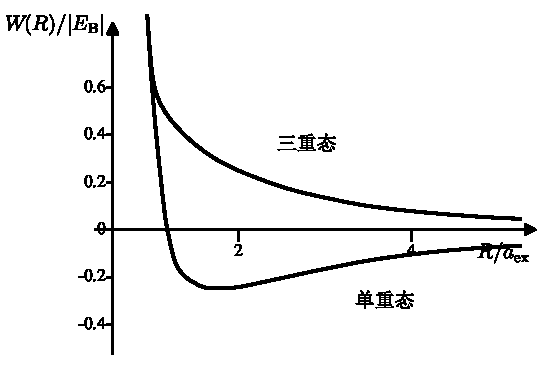
\includegraphics[width=6.5cm]{fig10-4.pdf}\\[0.2em]
{\small 图 10.4\quad $m_{\mathrm{h}}^{*}\gg m_{\mathrm{e}}^{*}$ 极限的双激子的互作用}\\[0.2em]
{\small （$|E_{\mathrm{B}}|\equiv e^{2}/(2\epsilon a_{\mathrm{ex}})$ 为瓦尼尔-莫特激子的结合能）}
\end{minipage}
\end{center}

双激子分子的基态波函数按海特勒-伦敦近似写为
\begin{equation}
\begin{aligned}
  \varPhi_{\mathrm{H}-\mathrm{L}}
  &=C_{\mathrm{s}}\left[\varphi_{\mathrm{a}}(1)\varphi_{\mathrm{b}}(2)
  +\varphi_{\mathrm{b}}(1)\varphi_{\mathrm{a}}(2)\right]\\
  &\quad\times\frac{1}{\sqrt{2}}\left[\chi_{\uparrow}(1)\chi_{\downarrow}(2)
  -\chi_{\downarrow}(1)\chi_{\uparrow}(2)\right]
\end{aligned}
\end{equation}
其中 $\chi_{\sigma}\left(\sigma=\uparrow,\downarrow\right)$ 代表自旋朝上和朝下态，而
\begin{equation}
  \varphi_{\mathrm{a}}(1)\equiv\pi^{-\frac{1}{2}}\exp\left(-r_{1\mathrm{a}}\right)
  \text{，}\qquad
  \varphi_{\mathrm{b}}(2)\equiv\pi^{-\frac{1}{2}}\exp\left(-r_{2\mathrm{b}}\right)
\end{equation}
是1s态激子的相对运动波函数，其中 $r_{1\mathrm{a}}$，$r_{2\mathrm{b}}$，…是以激子半径 $a_{\mathrm{ex}}$ 为单位的相对坐标.这样，在 $\sigma=0$ 极限双激子分子基态波函数的空间部分可写为
\begin{equation}
\begin{aligned}
  \psi_{\mathrm{H}-\mathrm{L}}&=(2C_{\mathrm{s}}/\pi)
  \exp\left[-(1/2)\left(r_{1\mathrm{a}}+r_{1\mathrm{b}}+r_{2\mathrm{a}}+r_{2\mathrm{b}}\right)\right]\\
  &\quad\times\cosh\left[-(1/2)\left(r_{1\mathrm{a}}-r_{1\mathrm{b}}-r_{2\mathrm{a}}+r_{2\mathrm{b}}\right)\right]
\end{aligned}
\end{equation}
上式中归一化参数 $C_{\mathrm{s}}$ 是R的函数.

\subsection*{(ii) $\sigma=1$ 极限}

这时 $m_{\mathrm{e}}^{*}=m_{\mathrm{h}}^{*}$，和氢分子问题差别很大，但与正电子素分子(positronium molecule)问题相似.惠勒(Wheeler)指出\textsuperscript{[6]}，用H-L型波函数不能求得两个正电子和两个负电子的束缚态(即正电子素分子).海勒拉斯(Hylleraas)和奥雷(Ore)引入下列试探函数\textsuperscript{[7]}（以下简称H-O函数）
\begin{equation}
\begin{aligned}
  \psi_{\mathrm{H}-\mathrm{O}}&=2\exp\left[-(1/2)\alpha
  \left(r_{1\mathrm{a}}+r_{1\mathrm{b}}+r_{2\mathrm{a}}+r_{2\mathrm{b}}\right)\right]\\
  &\quad\times\cosh\left[-(1/2)\beta\alpha
  \left(r_{1\mathrm{a}}-r_{1\mathrm{b}}-r_{2\mathrm{a}}+r_{2\mathrm{b}}\right)\right]
\end{aligned}
\end{equation}
其中 $\alpha$、$\beta$ 为可调参数，他们利用变分法算得了正电子素分子的结合能.沙尔玛(Sharma)\textsuperscript{[8]}将H-O函数用于双激子分子，证明了在 $\sigma=m_{\mathrm{e}}^{*}/m_{\mathrm{h}}^{*}=1$ 极限下也有稳定的分子结合，$\sigma=1$ 情况又称为正电子素分子极限.

\subsection*{(iii) $0<\sigma<1$ 情况}

作为一般情况的讨论，只需要研究 $\sigma$ 在0与1之间系统的性质，因为由于对称性 $\sigma>1$ 区域与 $\sigma<1$ 区是等效的，可以从 $\sigma<1$ 推知 $\sigma>1$ 情况，由此可得任意 $\sigma$ 比值的信息.阿达莫夫斯基(Adamowski)等\textsuperscript{[9]}仅仅从哈密顿量的结构就证明了 $0\leqslant\sigma\leqslant1$ 范围内激子分子的结合能与激子结合能之比只是 $\sigma$ 的单调衰减函数.因此，如果在 $\sigma=1$ 极限情况下证明了双激子分子的结合，则在 $0<\sigma<1$ 区域（以致全 $\sigma$ 区）内激子分子将是稳定的.从物理角度分析，阿达莫夫斯基的结论也是合理的.当 $\sigma$ 从零开始增大时，主要差别仅在于使空穴局域化必须增大动能，它随着 $\sigma$ 单调增加，从而降低结合能，到达 $\sigma=1$ 时结合能下降到最低值.对于 $\sigma>1$ 情况，可以将空穴当作“轻粒子”，电子当作“重粒子”重新定义 $\sigma$，作相似的讨论.

在这个区域中激子分子的结合能的定量计算主要由花村(Hanamura)\textsuperscript{[3]}和莱斯(Rice)\textsuperscript{[4]}两个小组作出，他们将H-O函数推广为
\begin{equation}
  \psi=f(R)g\left(\xi_{1},\eta_{1},\xi_{2},\eta_{2};R\right)
\end{equation}
这里
\begin{equation}
  f(R)=R^{\gamma/2}\exp\left(-\delta R/2\right)
\end{equation}
$g$ 就是 $\psi_{\mathrm{H}-\mathrm{O}}$ 的另一写法
\begin{equation}
  g=\exp\left[-(1/2)\alpha\left(\xi_{1}+\xi_{2}\right)R\right]
  \times\cosh\left[(1/2)\beta\alpha\left(\eta_{1}-\eta_{2}\right)R\right]
\end{equation}
$\alpha$、$\beta$、$\gamma$、$\delta$ 为独立变分参数，$\xi_{i}$ 和 $\eta_{i}\ (i=1,2)$ 由下列关系定义
\begin{equation}
  \xi_{i}=\left(r_{i\mathrm{a}}+r_{i\mathrm{b}}\right)/R
  \text{，}\qquad
  \eta_{i}=\left(r_{i\mathrm{a}}-r_{i\mathrm{b}}\right)/R
\end{equation}
这样写，是为了计算时便于运用旋转椭球坐标.当参数 $\gamma$ 和 $\delta$ 都趋向无穷大，且有固定比值 $(\gamma/\delta)=R_{0}$ 时，式(10.5.7)具有 $\delta\left(R-R_{0}\right)$ 函数特征，若再设 $\alpha=1$ 和 $\beta=-1$，则式(10.5.8)简化为(10.5.4)，这时 $\varPsi$ 代表固定 $R=R_{0}$ 值时的H-L近似波函数，可描述氢分子极限.如果令 $\gamma=\delta=0$，则 $f(R)=1$，$\varPsi=\psi_{\mathrm{H}-\mathrm{O}}$ 代表正电子素分子极限.这说明选择式(10.5.6)—(10.5.8)作为试探波函数是合理的.他们计算的结果由图10.5表示，正如阿达莫夫斯基所预料，激子分子的结合能与激子结合能的比值 $|E_{\mathrm{M}}|/|E_{\mathrm{B}}|$ 是 $\sigma$ 的单调衰减函数.

以上结果说明，对于电子和空穴有效质量比的任意值，双激子分子均是稳定的.同时，实验上也已证实在一系列半导体（如CuCl、CuBr、CdS、CdSe等)中均存在双激子分子.

双激子具有类玻色子特征，又由于它的平移质量很轻，因此双激子系统的量子效应可能比液氦更为显著.有许多理论工作者曾预言有双激子系统的玻色凝聚\textsuperscript{[3]}，但至今尚无确切的实验证明.

\begin{center}
\begin{minipage}{5.5cm}
\centering
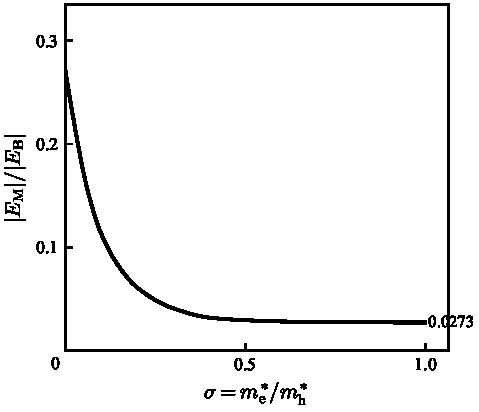
\includegraphics[width=5.5cm]{fig10-5.pdf}\\{\small 图 10.5\quad 激子分子结合能与 $\sigma$ 的关系}
\end{minipage}
\end{center}

\subsection*{2. 电子-空穴液体}

为了研究激子系统的相变，必须在本征半导体中产生高浓度的电子-空穴对激发.近年来利用皮秒激光(picosecond laser)技术，在非直接能隙半导体(如Ge、Si)中可以产生任意高浓度的激发，并观测到电子-空穴液滴.

从能带论角度讲，半导体可分为两类：一类是导带极小和价带极大（带边）具有相同的波矢值，称为直接能隙半导体，InSb、InAs、GaAs等属于这一类，它们的导带和价带边都在 $\boldsymbol{k}=0$ 处（Γ点）.另一类半导体其导带极小与价带极大的 $\boldsymbol{k}$ 值位于BZ中不同点，称为非直接能隙半导体，Ge、Si等属于非直接能隙半导体.在Ge晶体中价带边位于 $\boldsymbol{k}=0$（Γ点），但导带边在[111]方向的BZ边界的L点上 $\boldsymbol{k}=\frac{2\pi}{a}\left(\frac{1}{2},\frac{1}{2},\frac{1}{2}\right)$ 处，导带有4个等效的电子能量极小点，对应于四重简并，在极值附近的等能面是以[111]为轴的旋转椭球，平行和垂直转轴的有效质量分别为 $m_{\mathrm{eL}}^{*}=1.59m_{\mathrm{e}}$，和 $m_{\mathrm{eT}}^{*}=0.082m_{\mathrm{e}}$.Si的价带边也在Γ点，但导带边位于[100]方向上 $\frac{2\pi}{a}(0.86,0,0)$ 处（在BZ中Δ轴上靠近H点），等能面是以[100]为轴的旋转椭球，$m_{\mathrm{eL}}^{*}=0.92m_{\mathrm{e}}$，$m_{\mathrm{eT}}^{*}=0.19m_{\mathrm{e}}$，BZ内有6个等效的电子能量极小点，对应于六重简并，它们的能带曲线可参考文献\textsuperscript{[10]}.

在非直接能隙半导体中，因辐照激发的非平衡载流子(电子和空穴)将立刻弛豫到能带的极值处，库仑作用使它们形成激子，其中电子与空穴的波矢值不相同，这一特点要求非直接能隙半导体中激子的复合辐射必须有声子参加，否则就不能保持动量守恒.由于这个缘故，Ge和Si中激子的寿命可长达微秒量级，比非平衡载流子过渡到热平衡分布所需的时间(纳秒)长得多.所以，利用Ge、Si为背景材料，可以产生高浓度的、处于准平衡状态的激子系统，为激子相变的实验研究提供了条件.

只有在低浓度条件下，电子-空穴系统才可以看作是激子气体，在高浓度极限时，激子间的重叠十分强烈，以致使激子失去了它的个别特性，激子将离子化而不再作为一个确定的实体存在.1968年凯尔狄希(Keldysh)在第九届国际半导体会议上首先指出：高浓度条件下电子-空穴系统的最稳相可能是金属性的电子-空穴液体，这是由电子和空穴组成的二分量费密液体，简称为E-H液体.从此，理论工作者面临着一个课题，必须计算E-H液体中平均每个电子-空穴对的基态能量 $E_{\mathrm{G}}$，只有当 $|E_{\mathrm{G}}|$ 大于单激子结合能时，才能说明E-H液体是系统的稳定相.从多体理论角度讲，E-H液体的基态能由3部分组成：(i)电子系统和空穴系统的动能 $E_{\mathrm{K}}$，(ii)电子间和空穴间的交换能 $E_{\mathrm{ex}}$，(iii)相关能 $E_{\mathrm{corr}}$.为简便起见，先看各向同性非简并能带模型的计算结果；对于这种理想化的能带模型，电子与空穴的等能面都呈球形，因此依照电子体系理论［见式(4.9.14)］容易求得E-H液体中平均每个电子-空穴对的动能和交换能为
\begin{equation}
  E_{\mathrm{K}}=\frac{3}{5}\biggl(\frac{\hbar^{2}k_{\mathrm{F}}^{2}}{2m_{\mathrm{e}}^{*}}
  +\frac{\hbar^{2}k_{\mathrm{F}}^{2}}{2m_{\mathrm{h}}^{*}}\biggr)
  =\frac{3}{5}\frac{\hbar^{2}k_{\mathrm{F}}^{2}}{2\overline{M}}
  =\frac{2.21}{r_{\mathrm{s}}^{2}}\ [\text{激子 Ry}]
\end{equation}
\begin{equation}
  E_{\mathrm{ex}}=-\frac{3e^{2}k_{\mathrm{F}}}{2\pi}
  =-\frac{1.832}{r_{\mathrm{s}}}\ [\text{激子 Ry}]
\end{equation}
其中 $k_{\mathrm{F}}$ 为费密波矢，$\overline{M}$ 是电子-空穴对的折合质量.$r_{\mathrm{s}}$ 代表以激子半径 $a_{\mathrm{ex}}=\epsilon\hbar^{2}/(\overline{M}e^{2})$ 为单位的平均电子(或空穴)间距，它是和电子-空穴对浓度n有关的参数
\begin{equation}
  n=\frac{3}{4\pi r_{\mathrm{s}}^{3}a_{\mathrm{ex}}^{3}}
\end{equation}
式(10.5.10)和(10.5.11)的最后等式以单激子结合能 $|E_{\mathrm{B}}|=e^{2}/(2\epsilon a_{\mathrm{ex}})$ 为单位，称为激子的里德伯单位.对于相关能，花村\textsuperscript{[11]}用高密度展开法作了初步估计，当 $\sigma=1$ 时得到
\begin{equation}
  E_{\mathrm{corr}}=0.497\ln r_{\mathrm{s}}-0.33\ [\text{激子 Ry}]
\end{equation}
代入基态能公式，
\begin{equation}
\begin{aligned}
  E_{\mathrm{G}}\left(r_{\mathrm{s}}\right)&=E_{\mathrm{K}}+E_{\mathrm{ex}}+E_{\mathrm{corr}}\\
  &=2.21/r_{\mathrm{s}}^{2}-1.832/r_{\mathrm{s}}+0.497\ln r_{\mathrm{s}}-0.33\ [\text{激子 Ry}]
\end{aligned}
\end{equation}
根据上式所作能量-密度曲线的极小值在 $r_{\mathrm{s}}=1.7$ 处，对应的能量极值为 $E_{\mathrm{G}}=-0.38$.显然这个数值比单个激子的基态能 $-1$ 高得多，不能说明E-H液体是稳定相.随后有一系列工作严格计算相关能，所得的 $E_{\mathrm{G}}\left(r_{\mathrm{s}}\right)$ 曲线如图10.6中虚线所示，对于各向同性非简并能带模型的极小点在 $r_{\mathrm{s}}=1.95$ 处，$E_{\mathrm{G}}=-0.86$，仍然高于 $-1$，迄今最好的多体计算也不能证明 $E_{\mathrm{G}}<-1$\textsuperscript{[4]}.莱斯\textsuperscript{[12]}和诺齐尔斯(Nozieres)\textsuperscript{[13]}两个小组同时指出：必须考虑Ge、Si能带的简并和各向异性结构才能算得 $E_{\mathrm{G}}<-1$，从而证明了E-H液体是高浓度时系统的稳定相.他们计算的动能和交换能有解析表示，在激子里德伯单位中可写成：
\begin{equation}
  E_{\mathrm{K}}=\frac{0.468}{r_{\mathrm{s}}^{2}}\text{，}\quad
  E_{\mathrm{ex}}=-\frac{1.136}{r_{\mathrm{s}}}\ (\mathrm{Ge})
\end{equation}
\begin{equation}
  E_{\mathrm{K}}=\frac{0.727}{r_{\mathrm{s}}^{2}}\text{，}\quad
  E_{\mathrm{ex}}=-\frac{1.157}{r_{\mathrm{s}}}\ (\mathrm{Si})
\end{equation}
但是相关能只有数值结果.对于Ge，$E_{\mathrm{G}}\left(r_{\mathrm{s}}\right)$ 曲线由图10.6中实线表示，其极小点在 $r_{\mathrm{s}}=0.63$ 处，极小点能量 $E_{\mathrm{G}}=-2.0$ 与 $r_{\mathrm{s}}$ 相应的电子-空穴对浓度 $n_{0}\approx2\times10^{17}\ \mathrm{cm}^{-3}$，用通常单位表示的 $|E_{\mathrm{G}}|=5.3$ meV，这个数值比Ge中激子结合能 $|E_{\mathrm{B}}|=4.15$ meV大得多，说明在高浓度条件下Ge中E-H液体是系统的基态，对于Si也有相似的结果.将式(10.5.10)与（10.5.11）和式（10.5.15）与(10.5.16)相比较，可以看出能带的简并和各向异性所引起系统动能的减少比交换能的减少大得多，这有利于E-H液体的能量降低.

\begin{center}
\begin{minipage}{6.5cm}
\centering
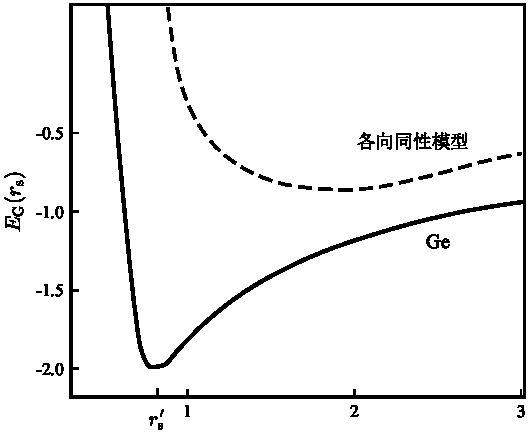
\includegraphics[width=6.5cm]{fig10-6.pdf}\\{\small 图 10.6\quad E-H液体的基态能的计算曲线\textsuperscript{[12,13]}}
\end{minipage}
\end{center}

在有限温度，当电子-空穴对的平均浓度小于 $n_{0}$ 时，E-H液体中将分离出低浓度的气相(激子气体)，并形成E-H液体和激子气体的两相共存区.这时，实验上就能观测到电子-空穴液滴.近年来，对于E-H液体的相图，应力、磁场等外界条件对E-H液体的影响，以及电子-空穴液滴的生长等问题都进行了系统研究\textsuperscript{[4,5]}.高密度条件下激子系统的相变问题已成为固体理论研究的新领域.

\begin{canKao}
\begin{enumerate}[label={[\arabic*]}, leftmargin=2.2em, itemsep=0pt]
\item Gross E F et al. Dokl Akad Nauk SSSR, 1953, 92: 265
\item Nakajima S et al. The Physics of Elementary Excitations. New York: Springer-Verlag, 1980. Chap 2
\item Hanamura E, Haug H. Phys Rep, 1977, 33C: 209
\item Rice T M. Solid State Phys, 1977, 32: 1
\item Hensel J C et al. Solid State Phys, 1977, 32: 88
\item Wheeler J A. Ann New York Acad Sci, 1946, 48: 219
\item Hylleraas E A, Ore A. Phys Rev, 1947, 71: 493, 913
\item Sharma R R. Phys Rev, 1968, 170: 770; 1968, 177: 36
\item Adamowski J A et al. Solid State Commun, 1971, 9: 2037; Phil Mag, 1972, 26: 143
\item Kittel C. Introduction to Solid State Physics. New York: Wiley, 1976. Chap 8
\item Hanamura E. Proc Int Conf Phys Semicond 10th. Virgina: Spring-field, 1970. 351
\item Brinkmann W F, Rice T M, Anderson P W, Chui S T. Phys Rev Lett, 1976, 28: 961; Phys Rev, 1973, B7: 1508
\item Combescot M, Nozieres P. J Phys, 1972, C5: 2369
\end{enumerate}
\end{canKao}

% ============================================================
%  第十一章 强关联电子体系（前半：§1–§6）
%  底本：高等教育出版社《固体理论》第二版；原书印刷页 390–432
%  （PDF 页 = 印刷页 + 20；§1 约印 390–402，§2 约印 402–411，
%   §3 印 411–415，§4 印 415–417，§5 印 417–426，§6 印 426–432）
%  后半 §7–§11 及章末参考文献见 ch11b.tex（原书第十一章文献在
%  §11 之后，印刷页 456 起）。
%  公式编号自检：§1 (11.1.1)–(11.1.65)；§2 (11.2.1)–(11.2.42)；
%    §3 (11.3.1)–(11.3.26)；§4 (11.4.1)–(11.4.13)；
%    §5 (11.5.1)–(11.5.42)；§6 (11.6.1)–(11.6.21)
%    （(11.6.6a/b)、(11.6.9a/b) 为原书自带二级编号，用
%    subequations 环境照录，与 ch04/ch06 体例一致）。
%    全半区自动编号 209 个，无缺号。
%
%  任务单所列 ch11 "缺号"（本半区相关者）逐条对照原书页面判定，
%  均非原书跳号，系 OCR 把 (11.x.y) 误作 (1.x.y)（少首位 1）或
%  编号碎裂，已按页面归还：
%    (11.1.38) tag 作 (1.1.38)（p395 在号）；
%    (11.1.45) 编号碎裂嵌于式内（p397），已归还；
%    (11.1.64) 编号以散字"(11.1.64)"混入式尾（p400），已归还；
%    (11.2.21) tag 作 (1.2.21)（p406 在号）；
%    (11.2.24) OCR 将 (11.2.23)/(11.2.24) 并成一块、只剩游离
%              "(11.2.24)"文字——原书 p406 为 ω±iη 两个独立编号
%              公式，已按页面拆为两式；
%    (11.2.26) 谱定理式编号碎裂（p407），已复原；
%    (11.2.27) tag 残作 (.27)（p407 在号），已归还；
%    (11.3.1)  tag 作 (1.3.1)（p412 在号）；
%    (11.3.12) tag 残作 (.12)（p413 在号），已归还；
%    (11.3.21) tag 残作 (21)（p414 在号），已归还；
%    (11.3.22) 编号碎裂（p415），已归还；
%    (11.4.4)  tag 作 (1.4.4)（p416 在号）；
%    (11.5.1)  编号碎裂混入正文（p417 在号），已排为编号公式；
%    (11.5.11) 编号碎裂（p420 在号），已归还；
%    (11.6.6)(11.6.9) 原书即分 a/b（p428、429），照录。
%    （任务单另一批"1.1/1.2/1.4/1.11 缺号"实为 (11.x.y) 之
%    OCR 误读，不属于本半区问题。）
%
%  已修正的 OCR/原书错误（除全角句点转"."、删 ~ 间隔符、收紧
%  \mathrm{d}、拆开行内公式与中文、函数名复原等常规项外）：
%  1. (11.1.2) 求和指标与算符按 p391 复原为 k₁,k₂,k'₁,k'₂ 及
%     C⁺_{k₁σ}C⁺_{k₂σ'}C_{k'₂σ'}C_{k'₁σ}（OCR 指标重复、"C⁻"
%     乱码）；(11.1.1) 两行原书一个编号，已合并。
%  2. (11.1.10)(11.1.13)(11.1.15) 中 n_{iσ}n_{iσ̄} 等按 p392 复原
%     （OCR 丢 σ̄ 杠）；(11.1.11) σ=↑,↓。
%  3. §1.1 末段 OCR"！T₁1正比于""ΔĒ比于""T₀\Δ"乱码，按 p392–393
%     复原为"不难证明|T₁|正比于…""宽度Δ正比于|T₁|""T₀、Δ（或
%     T₁）和U…其中T₁<0."。
%  4. (11.1.19) Z_G、T_r、ℋ=H−μN 按 p393 复原（OCR "≤X>、Z_6"
%     乱码）。
%  5. §1.2 正文 OCR"当它位于μ能带之中时"衍字符 μ，按 p394 删
%     （原书"当它位于能带之中时"）。
%  6. (11.1.23) 式尾杂符"(i)"已删（p394）。
%  7. (11.1.32)–(11.1.37) A=n_{iσ̄}C_{iσ}、n²_{iσ̄}=n_{iσ̄}、
%     <n_{iσ̄}> 及 δ_{ij} 按 p395 复原（OCR 的 S_{ij}、σ/σ̄ 混乱
%     等均已清）。
%  8. (11.1.41) 第四项带波浪号的算符 C⁺_{iσ̄}C_{lσ̄}−C⁺_{lσ̄}C_{iσ̄}
%     及正文对应平均值 (<C⁺_{iσ̄}C_{lσ̄}>−<C⁺_{lσ̄}C_{iσ̄}>) 按
%     p397 复原；式内波浪着重线未排（见遗留问题）。
%  9. (11.1.53)(11.1.56) 按 p398–399 复原为 E^(1)/E^(2)、
%     A^(1)/A^(2) 并列两支解（OCR 只剩残行、√ 内乱码）；
%     (11.1.55) 首行 A^{(i)}_{kσ}=∂E^{(i)}_{kσ}/∂E_k。
% 10. (11.1.57) 第二行按 p399 复原为 (i/2πN)Σ_k{G_k^σ(ω+iη)−
%     G_k^σ(ω−iη)}(η=+0)（OCR 严重乱码）。
% 11. §1.5 "(Δ/U)_c"之 OCR 上标 † 经 300dpi 放大核对为印刷噪声，
%     已删（p401）。
% 12. §2.1 V_kd 第二等式、"ℋ是单电子哈密顿量"补 ℋ；朗德因子
%     "g₀=g_i=2"按 p404 复原（OCR "θ0 σ=σ_{g_i}" 乱码）。
% 13. (11.2.8) 末项原书衍一"["，按第二套运动方程通式(11.2.11)
%     更正为 <<A(t);[B,H]>>（p405）。
% 14. (11.2.13)(11.2.16)(11.2.17)(11.2.20)(11.2.23)(11.2.24) 中
%     n_{dσ̄}、Ẽ_{dσ} 等上下标按 p405–406 复原；(11.2.18) 线性化
%     近似式按 p406 复原（OCR n_{dσ}n_{dσ}）。
% 15. p408"利用态密可以计算"→"利用态密度可以计算"（原书漏字，
%     补"度"）。
% 16. (11.2.45) "和 Γ/U={…}"之"和"按 p430 复原（OCR 作花体 ℋ）。
% 17. §2.4 图 11.7 图注 OCR 粘进行文（"当图 11.7 安德逊哈特利-
%     福克解的…区域"），按 p411 拆出图注，"当"字归回正文；
%     "周期性定德逊模型"→"周期性安德逊模型"（p411）。
% 18. (11.3.3) 按 p412 复原（OCR 引号/箭头乱码）；(11.3.8) 算符
%     上下标经 300dpi 放大核对复原为 C⁺_{kσ}C_{k'σ}C⁺_{nσ'}C_{nσ'}
%     与 C⁺_{kσ}C_{k'σ'}C⁺_{nσ'}C_{nσ}（p413）。
% 19. 原书 p413 "将交换项式(11.3.9)改写成"引号有误：交换项定义
%     于式(11.3.10)，已更正。
% 20. (11.3.11)(11.3.12) 两块严重乱码按 p413 重排复原；
%     (11.3.21)(11.3.22) 按 p414–415 复原（OCR 算符残缺）。
% 21. 原书 p415 "可将 s-d 互作用式(11.3.11)改写成"引号有误：
%     所改写的是已代入 J、U 的(11.3.21)，已更正。
% 22. 原书 p415 (11.3.25) 末算符印作 C⁺_{kμ}C⁺_{k'μ'}，第二个
%     上标 + 为衍符，按 (11.3.22) 更正为 C⁺_{kμ}C_{k'μ'}。
% 23. (11.4.11) 主值积分花体 𝒫 按 p417 复原（OCR 作 𝓡）。
% 24. 原书 p419 (11.5.10) 前因子印作 (J/S)²，按 (11.5.9) 更正为
%     (J/N)²（量纲与同式结构）。
% 25. (11.5.13)(11.5.14)(11.5.25)(11.5.32) 等 cases 中文条件
%     "（当…时）"按 p420、424、425 复原（OCR 乱码）。
% 26. (11.5.19)(11.5.20) 熵花体 𝒮 统一 \mathscr{S}；(11.5.21)
%     三式合排，χ_杂质、c_杂质 等中文下标以 \text{} 照排。
% 27. (11.5.35) "ΣΓ_k=常数"按 p425 复原（OCR "‡‡𝒳" 乱码）；
%     (11.5.40) 复原为 exp[−2/(|J|ρ_F)]（p425）。
% 28. 原书 p426 "必须同时考虑所有粒子相互用的真正多体问题"
%     漏字，补"作"作"相互作用"；原书 p422 "(贝本章§9)"为
%     "见"之误（与并行句"(见本章§10)"一致），已更正。
% 29. §5.3 末段 OCR "U>>T"→U>>Γ（Γ 为 (11.2.22) 定义的线宽，
%     p432）；"钢系"→"锕系"；"有效质量的m_e下界"衍 m_e 已删
%     （p452"有效质量的下界"）。
% 30. 原书 p428 "施里弗-沃尔夫变则只是在"漏字，补"换"作
%     "变换则只是"。
% 31. (11.6.9a)(11.6.9b) 按 p428–429 复原（OCR tag 残作"9b"）；
%     (11.6.11)(11.6.12) 按 p429 重排（OCR 的 C_{k't'} 类乱码
%     复原为 ↑/↓ 自旋指标）。
% 32. 原书 p430 (11.6.19) 首项印作 Ŝ（无上标），按 (11.6.16)
%     补 Ŝ^z；该式 OCR 严重乱码已按 p430 重排。
% 33. 原书 p426 §6 首句即以"讲的是如何…"起（承章题省略主语），
%     照录未改（见遗留问题）。
%  插图：图 11.1–图 11.14 共 14 幅（任务单所称"本半区含
%  图11.1–图11.7"有遗漏——图 11.8–图 11.14 亦在 §5–§6 区间内，
%  均已按原书页面排出）。
%  遗留问题：
%  · 图 11.1–11.14 均为占位图（figures/fig11-N.pdf），待重绘代理
%    按原书绘制；
%  · (11.1.41) 原书在带波浪号的算符部分下有"~~~"着重线，本稿
%    未排波浪线，仅以正文"有"~~~"号的算符部分"照录；
%  · §6 首句"讲的是如何从安德逊模型导出 s-d 交换模型"无主语，
%    原书如此（p426），照录；
%  · (11.1.23) 原书 δ 函数项中作 [A(t),B(t)]_+（p394），照录；
%  · (11.2.19) 第二个分母原书作 (ω−E_{k'σ})（与 (11.2.12)、
%    (11.2.15) 的同 σ 记号一致），照录。
% ============================================================
\chapter{强关联电子体系}

\section{赫伯德模型}

在小极化子理论中，我们已经看到当电子-声子互作用足够强时，离子晶体的电导不能用能带图像描述，而必须从局域模型出发建立小极化子的跳跃电导理论.这是能带论失效的一个例子，问题的关键是单电子近似忽略了电子-声子互作用对载流子状态的影响.

建立在单电子近似基础上的能带理论，不仅忽略了电子-声子互作用，而且还认为价电子在晶体中的运动是彼此独立的，因此电子间的关联作用也被忽略了.实际上在窄能带中电子间关联作用是十分重要的，因为电子从一个局域原子轨道运动到另一个原子局域轨道上时，必须考虑后一轨道是否被其它电子占据，如果已被占据，则应当计入在同一原子（或格点）周围两个电子间的库仑作用，这一作用将使能带状态发生显著的变化.

在实验上也发现，用能带论解释过渡金属化合物的特性往往是失败的.例如MnO晶体，平均每个元胞中有5个3d电子构成未填满的3d带，而O$^{2-}$的2p能带是满带，且与3d带不重叠.因此能带论说明MnO的3d带将具有金属导电性，但是测得的导电率很低，在室温下只有 $10^{-15}\,\Omega^{-1}\cdot\mathrm{cm}^{-1}$，说明MnO晶体实际上是绝缘体而不是导体，类似的情况也出现在高温超导的母体化合物如La$_{2}$CuO$_{4}$等之中.对于ReO$_{3}$，能带论预言它是绝缘体，但实际是良导体，其室温导电率为 $10^{5}\,\Omega^{-1}\cdot\mathrm{cm}^{-1}$ 与金属Cu差不多.还有些过渡金属氧化物当温度升高时会从绝缘体变为金属，这些都是能带论不能解释的.通过本节的讨论将明白，造成以上谬误的主要原因是能带论忽略了窄带中的电子强关联效应.

\subsection*{1. 赫伯德哈密顿量}

考虑N个原子组成的简单晶体，设 $h(\boldsymbol{r}_{i})$ 代表单电子在周期场中的哈密顿量，则多体系统的总哈密顿量为
\begin{equation}
\begin{aligned}
  &H=\sum_{i}h(\boldsymbol{r}_{i})
  +\frac{1}{2}\sum_{i,\,j}v_{ij}\\
  &v_{ij}=\frac{e^{2}}{|\boldsymbol{r}_{i}-\boldsymbol{r}_{j}|}
\end{aligned}
\end{equation}
为简单起见只考虑单个未填满的能带，例如孤立的s带.这时在布洛赫表象中互作用哈密顿量的二次量子化表示式可写成
\begin{equation}
  H=\sum_{k,\,\sigma}E_{k}C^{+}_{k\sigma}C_{k\sigma}
  +\frac{1}{2}\sum_{\substack{k_{1},\,k_{2},\,k'_{1},\,k'_{2}\\ \sigma,\,\sigma'}}
  \langle\,k_{1},k_{2}\mid v\mid k'_{1},k'_{2}\,\rangle\,
  C^{+}_{k_{1}\sigma}C^{+}_{k_{2}\sigma'}C_{k'_{2}\sigma'}C_{k'_{1}\sigma}
\end{equation}
其中 $E_{k}$ 是能带电子的能量，$C^{+}_{k\sigma}$ 和 $C_{k\sigma}$ 代表布洛赫轨道（k波矢）上 $\sigma$ 自旋电子的产生及消灭算符，而
\begin{equation}
  \langle\,k_{1},k_{2}\mid v\mid k'_{1},k'_{2}\,\rangle
  =e^{2}\int\frac{\psi^{*}_{k_{1}}(\boldsymbol{r})\psi^{*}_{k_{2}}(\boldsymbol{r}')
  \psi_{k'_{1}}(\boldsymbol{r})\psi_{k'_{2}}(\boldsymbol{r}')}
  {|\boldsymbol{r}-\boldsymbol{r}'|}\,\mathrm{d}\boldsymbol{r}\,\mathrm{d}\boldsymbol{r}'
\end{equation}
为了讨论窄带中关联问题，最好采用瓦尼尔表象，利用熟知的变换关系式
\begin{equation}
  \psi_{k}(\boldsymbol{r})=N^{-\frac{1}{2}}\sum_{i}
  \mathrm{e}^{\mathrm{i}\boldsymbol{k}\cdot\boldsymbol{R}_{i}}
  a(\boldsymbol{r}-\boldsymbol{R}_{i})
\end{equation}
和
\begin{equation}
\left.
\begin{aligned}
  &C^{+}_{i\sigma}=N^{-\frac{1}{2}}\sum_{k}
  \mathrm{e}^{-\mathrm{i}\boldsymbol{k}\cdot\boldsymbol{R}_{i}}C^{+}_{k\sigma}\\
  &C_{i\sigma}=N^{-\frac{1}{2}}\sum_{k}
  \mathrm{e}^{\mathrm{i}\boldsymbol{k}\cdot\boldsymbol{R}_{i}}C_{k\sigma}
\end{aligned}\right\}
\end{equation}
将式(11.1.2)变换到瓦尼尔表象
\begin{equation}
  H=\sum_{i,\,j}\sum_{\sigma}T_{ij}C^{+}_{i\sigma}C_{j\sigma}
  +\frac{1}{2}\sum_{\substack{i,\,j,\,l,\,m\\ \sigma,\,\sigma'}}
  \langle\,ij\mid v\mid lm\,\rangle\,
  C^{+}_{i\sigma}C^{+}_{j\sigma'}C_{m\sigma'}C_{l\sigma}
\end{equation}
其中 $C^{+}_{i\sigma}$ 和 $C_{i\sigma}$ 是瓦尼尔轨道（i格点）上 $\sigma$ 自旋电子的产生及消灭算符，单粒子项中
\begin{equation}
\begin{aligned}
  T_{ij}&=\int a^{*}(\boldsymbol{r}-\boldsymbol{R}_{i})h(\boldsymbol{r})
  a(\boldsymbol{r}-\boldsymbol{R}_{j})\,\mathrm{d}\boldsymbol{r}\\
  &=N^{-1}\sum_{k}\mathrm{e}^{\mathrm{i}\boldsymbol{k}\cdot(\boldsymbol{R}_{i}-\boldsymbol{R}_{j})}E_{k}
\end{aligned}
\end{equation}
互作用项中
\begin{equation}
  \langle\,ij\mid v\mid lm\,\rangle
  =e^{2}\int\frac{a^{*}(\boldsymbol{r}-\boldsymbol{R}_{i})
  a^{*}(\boldsymbol{r}'-\boldsymbol{R}_{j})
  a(\boldsymbol{r}-\boldsymbol{R}_{l})a(\boldsymbol{r}'-\boldsymbol{R}_{m})}
  {|\boldsymbol{r}-\boldsymbol{r}'|}\,\mathrm{d}\boldsymbol{r}\,\mathrm{d}\boldsymbol{r}'
\end{equation}
式(11.1.8)一般为多中心积分，但可简化为单中心、双中心等积分.赫伯德指出\textsuperscript{[1]}，对于窄带单中心积分
\begin{equation}
  \langle\,ii\mid v\mid ii\,\rangle\equiv U
  =e^{2}\int\frac{a^{*}(\boldsymbol{r}-\boldsymbol{R}_{i})
  a^{*}(\boldsymbol{r}'-\boldsymbol{R}_{i})
  a(\boldsymbol{r}-\boldsymbol{R}_{i})a(\boldsymbol{r}'-\boldsymbol{R}_{i})}
  {|\boldsymbol{r}-\boldsymbol{r}'|}\,\mathrm{d}\boldsymbol{r}\,\mathrm{d}\boldsymbol{r}'
\end{equation}
是最重要的，它代表同一格点（或原子）周围能带电子之间的库仑作用，这是近距离的作用，其数量级约为10eV，比双中心、三中心等积分的贡献大得多.作为一个简单的模型，可以略去互作用项中所有的多中心积分，只取单中心积分项，这就是赫伯德模型（Hubbard model）.因此，互作用项近似为
\begin{equation}
  \frac{1}{2}U\sum_{i}\sum_{\sigma,\,\sigma'}
  C^{+}_{i\sigma}C^{+}_{i\sigma'}C_{i\sigma'}C_{i\sigma}
  =\frac{1}{2}U\sum_{i}\sum_{\sigma}n_{i\sigma}n_{i\bar{\sigma}}
\end{equation}
其中
\begin{equation}
  \bar{\sigma}\equiv-\sigma\qquad(\sigma=\uparrow,\,\downarrow)
\end{equation}
而
\begin{equation}
  n_{i\sigma}=C^{+}_{i\sigma}C_{i\sigma}
\end{equation}
代表在i格点上 $\sigma$ 自旋的粒子数算符.在式(11.1.10)中利用了泡利原理，即不可能在同一格点i上产生两个自旋取向相同的电子，因此必须 $\sigma'=\bar{\sigma}$.将式(11.1.6)右边第二项近似用式(11.1.10)的右边项表示，就得到赫伯德哈密顿量
\begin{equation}
  H=\sum_{i,\,j}\sum_{\sigma}T_{ij}C^{+}_{i\sigma}C_{j\sigma}
  +\frac{U}{2}\sum_{i}\sum_{\sigma}n_{i\sigma}n_{i\bar{\sigma}}
\end{equation}
应当注意，在赫伯德模型中所计入的关联相反自旋电子之间的排斥势U对于金属-绝缘体相变以及窄带磁性均有重要影响.根据式(11.1.7)，H的单粒子部分中 $j=i$ 项的系数为
\begin{equation}
  T_{ii}=N^{-1}\sum_{k}E_{k}\equiv T_{0}
\end{equation}
它代表能带电子的平均能量.当 $\boldsymbol{R}_{j}-\boldsymbol{R}_{i}=\boldsymbol{R}_{l}$ 为最近邻格点间位矢差时，$T_{ij}\equiv T_{1}$.不难证明 $|T_{1}|$ 正比于紧束缚近似的能带宽度 $\Delta$.例如，令式(11.1.13)中 $U=0$，我们将得到紧束缚近似哈密顿量为
\begin{equation}
  H_{0}=\sum_{i,\,j}\sum_{\sigma}T_{ij}C^{+}_{i\sigma}C_{j\sigma}
  \approx T_{0}\sum_{i,\,\sigma}C^{+}_{i\sigma}C_{i\sigma}
  +T_{1}\sum_{l}^{(n.n.)}\sum_{i,\,\sigma}C^{+}_{i\sigma}C_{i+l,\,\sigma}
\end{equation}
利用变换式(11.1.5)将 $H_{0}$ 变回布洛赫表象，求得
\begin{equation}
  H_{0}\approx\sum_{k,\,\sigma}\Bigl(T_{0}
  +T_{1}\sum_{l}^{(n.n.)}\mathrm{e}^{-\mathrm{i}\boldsymbol{k}\cdot\boldsymbol{R}_{l}}\Bigr)
  C^{+}_{k\sigma}C_{k\sigma}
  =\sum_{k,\,\sigma}E_{k}C^{+}_{k\sigma}C_{k\sigma}
\end{equation}
其中
\begin{equation}
  E_{k}\approx T_{0}+T_{1}\sum_{l}^{(n.n.)}
  \mathrm{e}^{-\mathrm{i}\boldsymbol{k}\cdot\boldsymbol{R}_{l}}
\end{equation}
这就是紧束缚近似的能带电子能量，其能带的宽度 $\Delta$ 正比于 $|T_{1}|$.因此，$T_{0}$、$\Delta$（或 $T_{1}$）和U是赫伯德模型的3个重要参数，其中 $T_{1}<0$.下面将分别 $\Delta=0$ 和 $\Delta\neq0$ 情况讨论赫伯德模型的解.

\subsection*{2. 双时格林函数的运动方程方法\textsuperscript{[2]}}

我们将利用双时格林函数方法求解赫伯德哈密顿量式(11.1.13)的能级和态密度，为此读者应参考附录C中的祖巴列夫（Zubarev）的格林函数运动方程法.

将附录A中所介绍的双时推迟格林函数用于电子系统，定义推迟格林函数：
\begin{equation}
\begin{aligned}
  \langle\langle A(t);B(t')\rangle\rangle
  &=-\mathrm{i}\theta(t-t')\langle[A(t),B(t')]_{+}\rangle\\
  &=-\mathrm{i}\theta(t-t')\bigl\{\langle A(t)B(t')\rangle
  +\langle B(t')A(t)\rangle\bigr\}
\end{aligned}
\end{equation}
其中 $\theta(t-t')$ 为阶跃函数：
\begin{equation*}
  \theta(t-t')=\begin{cases}1&(t>t')\\0&(t<t')\end{cases}
\end{equation*}
$A(t)$ 为海森伯绘景中算符 $\mathrm{e}^{\mathrm{i}Ht}A\mathrm{e}^{-\mathrm{i}Ht}$，这里取 $\hbar=1$ 单位，$\langle\cdots\rangle$ 代表巨正则系综平均
\begin{equation}
\begin{aligned}
  &\langle X\rangle=Z^{-1}_{\mathrm{G}}\mathrm{Tr}
  \bigl(\mathrm{e}^{-\beta\mathscr{H}}X\bigr),
  \qquad Z_{\mathrm{G}}=\mathrm{Tr}\bigl(\mathrm{e}^{-\beta\mathscr{H}}\bigr)\\
  &\mathscr{H}=H-\mu N
\end{aligned}
\end{equation}
$Z_{\mathrm{G}}$ 是配分函数，$\mu$ 为化学势.式(11.1.18)中取(+)号是由于A和B为费密算子，满足反对易律.当H与时间无关时，$\langle\langle A(t);B(t')\rangle\rangle$ 只是时间差 $(t-t')$ 的函数，可令 $t'=0$，而讨论格林函数 $\langle\langle A(t);B(0)\rangle\rangle$，其傅里叶变换为
\begin{equation}
  \langle\langle A\mid B\rangle\rangle_{\omega+\mathrm{i}\eta}
  =\int_{-\infty}^{\infty}\mathrm{d}t\,
  \langle\langle A(t);B(0)\rangle\rangle
  \exp\bigl[\mathrm{i}(\omega+\mathrm{i}\eta)t\bigr]
  \qquad(\eta=+0)
\end{equation}
代表上半复平面的格林函数，在附录A中已证明格林函数 $\langle\langle A\mid B\rangle\rangle_{\omega}$ 与平均量 $\langle BA\rangle$ 在采用巨正则系综时的关系为
\begin{equation}
  \langle\,BA\,\rangle=\frac{\mathrm{i}}{2\pi}
  \int_{-\infty}^{\infty}
  \frac{\langle\langle A\mid B\rangle\rangle_{\omega+\mathrm{i}\eta}
  -\langle\langle A\mid B\rangle\rangle_{\omega-\mathrm{i}\eta}}
  {\mathrm{e}^{\beta(\omega-\mu)}+1}\,\mathrm{d}\omega
\end{equation}
此即附录A中式(A.28)，这个公式在格林函数理论中称为谱定理.假如格林函数 $\langle\langle A\mid B\rangle\rangle_{\omega}$ 已解出，利用谱定理即可确定平均值 $\langle BA\rangle$.例如，从 $\langle\langle C_{k\sigma}\mid C^{+}_{k\sigma}\rangle\rangle_{\omega}$ 可决定准粒子数 $\langle C^{+}_{k\sigma}C_{k\sigma}\rangle$.还应当注意，在谱定理式(11.1.21)中的化学势 $\mu$ 应由总粒子数条件自洽决定，当它位于能带之中时系统为金属，而处于禁带（即能带隙）中时系统属于绝缘体.

问题是如何求解格林函数？对于双时推迟格林函数最简便的方法是建立运动方程.从式(11.1.18)出发，对t求导数，并利用海森伯运动方程
\begin{equation}
  \mathrm{i}\frac{\mathrm{d}A(t)}{\mathrm{d}t}=[A(t),H]
  =A(t)H-HA(t)
\end{equation}
求出格林函数的运动方程\textsuperscript{[2]}
\begin{equation}
  \mathrm{i}\frac{\mathrm{d}}{\mathrm{d}t}
  \langle\langle A(t);B(t')\rangle\rangle
  =\delta(t-t')\langle[A(t),B(t)]_{+}\rangle
  +\langle\langle[A(t),H];B(t')\rangle\rangle
\end{equation}
按照式(11.1.20)对上式作傅里叶变换，可将 $\langle\langle[A,H]\rangle\rangle_{\omega}$ 的运动方程写为
\begin{equation}
  \omega\langle\langle A\mid B\rangle\rangle_{\omega}
  =\langle[A,B]_{+}\rangle
  +\langle\langle[A,H]\mid B\rangle\rangle_{\omega}
\end{equation}
其中 $\langle\langle[A,H]\mid B\rangle\rangle_{\omega}$ 是高阶格林函数，它的运动方程仍为式(11.1.24)，只不过将A代以 $[A,H]$.因此，式(11.1.24)实际上是一组无穷长锁链方程的通式，详细的讨论见附录C.具体求解时，往往需要对高阶格林函数作某种近似（切断近似），使式(11.1.24)所决定的格林函数方程组近似成为封闭的形式，从而可用代数方法解出 $\langle\langle A\mid B\rangle\rangle_{\omega}$.在某些简单问题中，方程自动封闭，这时所求出格林函数是严格的.下面将格林函数的运动方程解法具体用于赫伯德模型.

\subsection*{3. 零能带宽度时赫伯德模型的严格解}

能带宽度 $\Delta=0$ 相当于在赫伯德哈密顿量中令
\begin{equation}
  T_{ij}=T_{0}\delta_{ij}
\end{equation}
根据式(11.1.13)，这时系统的哈密顿量可写成
\begin{equation}
  H=T_{0}\sum_{i,\,\sigma}n_{i\sigma}
  +\frac{1}{2}U\sum_{i,\,\sigma}n_{i\sigma}n_{i\bar{\sigma}}
\end{equation}
上式实为对角形式，利用格林函数可求出严格解.

定义单粒子格林函数
\begin{equation}
  G^{\sigma}_{ij}(\omega)\equiv
  \langle\langle C_{i\sigma}\mid C^{+}_{j\sigma}\rangle\rangle_{\omega}
\end{equation}
其运动方程根据式(11.1.24)为
\begin{equation}
  \omega\langle\langle C_{i\sigma}\mid C^{+}_{j\sigma}\rangle\rangle_{\omega}
  =\langle[C_{i\sigma},C^{+}_{j\sigma}]_{+}\rangle
  +\langle\langle[C_{i\sigma},H]\mid C^{+}_{j\sigma}\rangle\rangle_{\omega}
\end{equation}
其中
\begin{equation}
  [C_{i\sigma},H]=T_{0}C_{i\sigma}+UC_{i\sigma}n_{i\bar{\sigma}}
\end{equation}
再利用费密算子的对易式
\begin{equation}
  [C_{i\sigma},C^{+}_{j\sigma}]_{+}=\delta_{ij}
\end{equation}
可将方程(11.1.28)简化为
\begin{equation}
  (\omega-T_{0})\langle\langle C_{i\sigma}\mid C^{+}_{j\sigma}\rangle\rangle_{\omega}
  =\delta_{ij}
  +U\langle\langle n_{i\bar{\sigma}}C_{i\sigma}\mid C^{+}_{j\sigma}\rangle\rangle_{\omega}
\end{equation}
从上式可知，$\langle\langle C_{i\sigma}\mid C^{+}_{j\sigma}\rangle\rangle_{\omega}$ 由高阶格林函数 $\langle\langle n_{i\bar{\sigma}}C_{i\sigma}\mid C^{+}_{j\sigma}\rangle\rangle_{\omega}$ 决定.因此，为了求出单粒子格林函数 $G^{\sigma}_{ij}(\omega)$，还必须建立高阶格林函数
\begin{equation}
  \Gamma^{\sigma}_{ij}(\omega)\equiv
  \langle\langle n_{i\bar{\sigma}}C_{i\sigma}\mid C^{+}_{j\sigma}\rangle\rangle_{\omega}
\end{equation}
的运动方程.这时可设 $A=n_{i\bar{\sigma}}C_{i\sigma}$ 和 $B=C^{+}_{j\sigma}$，代入格林函数的通式(11.1.24)得到方程
\begin{equation}
  \omega\langle\langle n_{i\bar{\sigma}}C_{i\sigma}\mid C^{+}_{j\sigma}\rangle\rangle_{\omega}
  =\langle[n_{i\bar{\sigma}}C_{i\sigma},C^{+}_{j\sigma}]_{+}\rangle
  +\langle\langle[n_{i\bar{\sigma}}C_{i\sigma},H]\mid C^{+}_{j\sigma}\rangle\rangle_{\omega}
\end{equation}
再利用
\begin{equation*}
  [n_{i\bar{\sigma}},H]=0
\end{equation*}
和式(11.1.29)求出 $\Gamma^{\sigma}_{ij}(\omega)$ 的方程
\begin{equation}
  (\omega-T_{0})\Gamma^{\sigma}_{ij}(\omega)
  =\langle n_{i\bar{\sigma}}\rangle\delta_{ij}
  +U\langle\langle n^{2}_{i\bar{\sigma}}C_{i\sigma}\mid C^{+}_{j\sigma}\rangle\rangle_{\omega}
\end{equation}
由于费密子满足算符等式
\begin{equation}
  n^{2}_{i\bar{\sigma}}=n_{i\bar{\sigma}}
\end{equation}
因此式(11.1.34)右边第二项仍为 $\Gamma^{\sigma}_{ij}(\omega)$，方程组到 $\Gamma^{\sigma}_{ij}$ 已封闭，可严格解出
\begin{equation}
  \Gamma^{\sigma}_{ij}(\omega)
  =\delta_{i,\,j}\frac{\langle n_{i\bar{\sigma}}\rangle}{\omega-T_{0}-U}
\end{equation}
代入式(11.1.31)，最后求得单粒子格林函数
\begin{equation}
  G^{\sigma}_{ij}(\omega)=\delta_{ij}
  \left\{\frac{1-\langle n_{i\bar{\sigma}}\rangle}{\omega-T_{0}}
  +\frac{\langle n_{i\bar{\sigma}}\rangle}{\omega-T_{0}-U}\right\}
\end{equation}
利用谱定理公式(11.1.21)，由对角格林函数可确定每个格点上 $\sigma$ 自旋电子的平均数为
\begin{equation}
\begin{aligned}
  n_{\sigma}&\equiv\frac{1}{N}\sum_{j}
  \langle\,C^{+}_{j\sigma}C_{j\sigma}\,\rangle\\
  &=\int_{-\infty}^{\infty}\mathrm{d}\omega\,f(\omega)
  \frac{\mathrm{i}}{2\pi N}\sum_{j}
  \bigl\{G^{\sigma}_{jj}(\omega+\mathrm{i}\eta)
  -G^{\sigma}_{jj}(\omega-\mathrm{i}\eta)\bigr\}\\
  &=\int_{-\infty}^{\infty}\mathrm{d}\omega\,f(\omega)\rho_{\sigma}(\omega)
\end{aligned}
\end{equation}
这里 $f(\omega)=\{\exp[\beta(\omega-\mu)]+1\}^{-1}$ 是费密分布函数，$\rho_{\sigma}(\omega)$ 代表平均每个格点上 $\sigma$ 自旋电子的态密度，称为局域态密度.由式(11.1.38)可知，局域态密度为
\begin{equation}
\begin{aligned}
  \rho_{\sigma}(\omega)&=\frac{\mathrm{i}}{2\pi N}\sum_{j}
  \bigl\{G^{\sigma}_{jj}(\omega+\mathrm{i}\eta)
  -G^{\sigma}_{jj}(\omega-\mathrm{i}\eta)\bigr\}\\
  &=(1-\langle n_{\bar{\sigma}}\rangle)\delta(\omega-T_{0})
  +\langle n_{\bar{\sigma}}\rangle\delta(\omega-T_{0}-U)
\end{aligned}
\end{equation}
当系统具有平移不变性时，$\langle n_{i\bar{\sigma}}\rangle$ 应与格点位置无关，可令 $\langle n_{i\bar{\sigma}}\rangle=\langle n_{\bar{\sigma}}\rangle$.这时 $\langle n_{\bar{\sigma}}\rangle$ 为任一格点上 $\bar{\sigma}$ 自旋粒子的占据数，而 $(1-\langle n_{\bar{\sigma}}\rangle)$ 则代表其未占据数.因此式(11.1.39)说明，当 $\Delta=0$ 时赫伯德模型中每格点上电子有两个能级 $T_{0}$ 和 $T_{0}+U$，它们正好是格林函数 $G^{\sigma}_{ij}(\omega)$ 的两个极点，具体可从式(11.1.37)看出.当格点未被占据时，束缚一个 $\sigma$ 自旋的电子需 $T_{0}$ 能量，而当格点上已占据了一个 $\bar{\sigma}$ 自旋的电子时，$\sigma$ 自旋电子只能占据 $T_{0}+U$ 能级.或者说，在一格点周围束缚第二个电子（其自旋与原有电子相反）所需能量为 $T_{0}+U$，因为两自旋相反电子在同一格点附近的库仑排斥作用能为U.

若系统还具有自旋的朝上与朝下对称性，则可令 $\langle n_{\sigma}\rangle=\langle n_{\bar{\sigma}}\rangle=\dfrac{1}{2}n$，这里n代表平均每个格点上的电子数.对于半满带情况 $n=1$，系统的基态如图11.1(a)，N个电子恰好将各格点上的 $T_{0}$ 能级占满.半满赫伯德模型的第一激发如图11.1(b)所示，在两个能级均被占据的格点上有一对自旋取向相反的电子.

\begin{center}
\begin{minipage}{7cm}
\centering
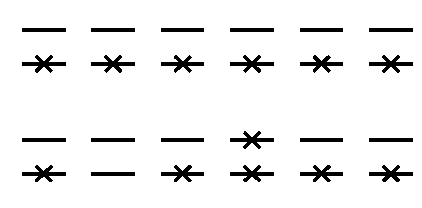
\includegraphics[width=7cm]{fig11-1.pdf}\\[0.3em]
{\small (a) 基态\qquad\qquad (b) 第一激发态}\\[0.2em]
{\small 图 11.1\quad $\Delta=0$ 时半满赫伯德模型的能态}
\end{minipage}
\end{center}

以上结果只是孤立原子系统的严格解.假如各格点上原子轨道波函数彼此重叠，则电子将在整个晶体中运动，并分别形成以 $T_{0}$ 为中心和以 $T_{0}+U$ 为中心的两个子带.当 $n=1$ 时，电子只填满 $T_{0}$ 子带，而 $T_{0}+U$ 子带则是空带，这时晶体是绝缘体.如果原子波函数重叠很厉害，则合并为一个半满能带，晶体是良导体.在中间情况，可能发生金属-绝缘体相变.

\subsection*{4. 窄带中的强关联效应}

当能带宽度 $\Delta\neq0$ 时，我们必须从严格的赫伯德哈密顿量［式(11.1.13)］出发，计入 $T_{ij}(j\neq i)$ 项.由于H不再是 $n_{i\sigma}$ 的对角型，利用格林函数方法只能求得近似解.

现在具体讨论 $\Delta\neq0$ 时的格林函数方程式(11.1.28)和式(11.1.33).从H的表示式(11.1.13)计算出下列对易式：
\begin{equation}
  [C_{i\sigma},H]=\sum_{j}T_{ij}C_{j\sigma}+Un_{i\bar{\sigma}}C_{i\sigma}
\end{equation}
\begin{equation}
\begin{aligned}
  \relax[n_{i\bar{\sigma}}C_{i\sigma},H]&=Un_{i\bar{\sigma}}C_{i\sigma}
  +T_{0}n_{i\bar{\sigma}}C_{i\sigma}
  +\sum_{l(l\neq i)}T_{il}\,n_{i\bar{\sigma}}C_{l\sigma}\\
  &\quad+\sum_{l}T_{il}
  \bigl(C^{+}_{i\bar{\sigma}}C_{l\bar{\sigma}}
  -C^{+}_{l\bar{\sigma}}C_{i\bar{\sigma}}\bigr)C_{i\sigma}
\end{aligned}
\end{equation}
将以上结果代入式(11.1.28)和(11.1.33)，所得到的运动方程并不封闭，因为式(11.1.41)中含交迭积分的项使 $\Gamma^{\sigma}_{ij}(\omega)$ 方程中出现三格点高阶格林函数.在窄带强关联情况下，为了使方程封闭，可以对这些项作如下近似处理：将式(11.1.41)右边有"~~~"号的算符部分近似用各自的平均值 $\langle n_{\bar{\sigma}}\rangle$ 和 $(\langle C^{+}_{i\bar{\sigma}}C_{l\bar{\sigma}}\rangle-\langle C^{+}_{l\bar{\sigma}}C_{i\bar{\sigma}}\rangle)$ 代替.由于 $E_{k}=E_{-k}$，可证明 $T_{il}=T_{li}$，再利用平移对称性将有
\begin{equation*}
  \sum_{l}T_{il}\bigl(\langle C^{+}_{i\bar{\sigma}}C_{l\bar{\sigma}}\rangle
  -\langle C^{+}_{l\bar{\sigma}}C_{i\bar{\sigma}}\rangle\bigr)=0
\end{equation*}
按照这样的近似方案，式(11.1.41)右边第四项的贡献为零，而第三项则给出 $G^{\sigma}_{lj}(\omega)$，这就是切断近似.由此求出近似封闭的格林函数方程组：
\begin{equation}
  \omega G^{\sigma}_{ij}(\omega)=\delta_{ij}
  +\sum_{l}T_{il}G^{\sigma}_{lj}(\omega)+U\Gamma^{\sigma}_{ij}(\omega)
\end{equation}
\begin{equation}
  \omega\Gamma^{\sigma}_{ij}(\omega)=\langle n_{\bar{\sigma}}\rangle\delta_{ij}
  +\langle n_{\bar{\sigma}}\rangle\sum_{l(l\neq i)}T_{il}G^{\sigma}_{lj}(\omega)
  +(T_{0}+U)\Gamma^{\sigma}_{ij}(\omega)
\end{equation}
由式(11.1.43)可解出
\begin{equation}
  \Gamma^{\sigma}_{ij}(\omega)=\frac{\langle n_{\bar{\sigma}}\rangle}{\omega-T_{0}-U}
  \Bigl\{\delta_{ij}+\sum_{l(l\neq i)}T_{il}G^{\sigma}_{lj}(\omega)\Bigr\}
\end{equation}
代入式(11.1.42)，得到单粒子格林函数方程
\begin{equation}
\begin{aligned}
  \omega G^{\sigma}_{ij}(\omega)&=T_{0}G^{\sigma}_{ij}(\omega)
  +\biggl\{1+\frac{U\langle n_{\bar{\sigma}}\rangle}{\omega-T_{0}-U}\biggr\}
  \bigl\{\delta_{ij}+\sum_{l(l\neq i)}T_{il}G^{\sigma}_{lj}\bigr\}\\
  &\qquad(i,\,j=1,\,2,\,\cdots,\,N)
\end{aligned}
\end{equation}
式(11.1.45)是格点格林函数 $G^{\sigma}_{ij}$ 的 $(N\times N)$ 矩阵方程，可利用表象变换求解.对于平移不变的系统，格点格林函数 $G^{\sigma}_{ij}$ 只是 $(\boldsymbol{R}_{i}-\boldsymbol{R}_{j})$ 的函数.这时利用变换式(11.1.5)可证明在布洛赫表象中单粒子格林函数是对角的，即
\begin{equation}
\begin{aligned}
  G^{\sigma}_{kk'}(\omega)&\equiv
  \langle\langle C_{k\sigma}\mid C^{+}_{k'\sigma}\rangle\rangle_{\omega}
  =N^{-1}\sum_{i,\,j}\mathrm{e}^{-\mathrm{i}\boldsymbol{k}\cdot\boldsymbol{R}_{i}}
  \mathrm{e}^{\mathrm{i}\boldsymbol{k}'\cdot\boldsymbol{R}_{j}}
  \langle\langle C_{i\sigma}\mid C^{+}_{j\sigma}\rangle\rangle_{\omega}\\
  &=\delta_{kk'}\langle\langle C_{k\sigma}\mid C^{+}_{k\sigma}\rangle\rangle_{\omega}
  \equiv\delta_{kk'}G^{\sigma}_{k}(\omega)
\end{aligned}
\end{equation}
其中 $G^{\sigma}_{k}(\omega)$ 是布洛赫表象中的对角格林函数 $\langle\langle C_{k\sigma}\mid C^{+}_{k\sigma}\rangle\rangle_{\omega}$.因此有傅里叶变换式
\begin{equation}
\begin{aligned}
  G^{\sigma}_{ij}(\omega)&=\frac{1}{N}\sum_{k}\sum_{k'}
  \mathrm{e}^{\mathrm{i}\boldsymbol{k}\cdot\boldsymbol{R}_{i}}
  \mathrm{e}^{-\mathrm{i}\boldsymbol{k}'\cdot\boldsymbol{R}_{j}}
  G^{\sigma}_{kk'}(\omega)\\
  &=\frac{1}{N}\sum_{k}\mathrm{e}^{\mathrm{i}\boldsymbol{k}\cdot(\boldsymbol{R}_{i}-\boldsymbol{R}_{j})}
  G^{\sigma}_{k}(\omega)
\end{aligned}
\end{equation}
利用上式以及式(11.1.7)的逆变换
\begin{equation}
  E_{k}=\frac{1}{N}\sum_{i,\,j}T_{ij}
  \mathrm{e}^{-\mathrm{i}\boldsymbol{k}\cdot(\boldsymbol{R}_{i}-\boldsymbol{R}_{j})}
\end{equation}
不难将式(11.1.45)对角化为格林函数 $G^{\sigma}_{k}(\omega)$ 的简单代数方程
\begin{equation}
  \omega G^{\sigma}_{k}(\omega)=T_{0}G^{\sigma}_{k}(\omega)
  +\biggl\{1+\frac{U\langle n_{\bar{\sigma}}\rangle}{\omega-T_{0}-U}\biggr\}
  \bigl\{1+(E_{k}-T_{0})G^{\sigma}_{k}(\omega)\bigr\}
\end{equation}
由此解出单粒子格林函数
\begin{equation}
  G^{\sigma}_{k}(\omega)=
  \frac{\omega-T_{0}-U(1-\langle n_{\bar{\sigma}}\rangle)}
  {(\omega-E_{k})(\omega-T_{0}-U)+\langle n_{\bar{\sigma}}\rangle U(T_{0}-E_{k})}
\end{equation}
为了讨论这个解的特点，将上式整理成下列标准形式：
\begin{equation}
  G^{\sigma}_{k}(\omega)=\frac{A^{(1)}_{k\sigma}}{\omega-E^{(1)}_{k\sigma}}
  +\frac{A^{(2)}_{k\sigma}}{\omega-E^{(2)}_{k\sigma}}
\end{equation}
其中 $E^{(1)}_{k\sigma}$ 和 $E^{(2)}_{k\sigma}$ 是格林函数 $G^{\sigma}_{k}(\omega)$ 之极点，由式(11.1.50)的分母等于零确定，即是下列二次方程的根
\begin{equation}
  (\omega-E_{k})(\omega-T_{0}-U)
  +\langle n_{\bar{\sigma}}\rangle(T_{0}-E_{k})U=0
\end{equation}
由此求出
\begin{equation}
\left.
\begin{aligned}
  &E^{(1)}_{k\sigma}\\
  &E^{(2)}_{k\sigma}
\end{aligned}\right\}
  =\frac{1}{2}\Bigl\{E_{k}+U+T_{0}
  \mp\sqrt{(E_{k}-U-T_{0})^{2}+4U\langle n_{\bar{\sigma}}\rangle(E_{k}-T_{0})}\Bigr\}
\end{equation}
并且
\begin{equation}
  E^{(1)}_{k\sigma}<T_{0}+U(1-\langle n_{\bar{\sigma}}\rangle)
  <E^{(2)}_{k\sigma}
\end{equation}
说明两支解不相交.系数 $A^{(i)}_{k\sigma}(i=1,\,2)$ 由式(11.1.50)和式(11.1.51)决定，有关系式
\begin{equation}
\begin{aligned}
  &A^{(i)}_{k\sigma}=\frac{\partial E^{(i)}_{k\sigma}}{\partial E_{k}}
  \qquad(i=1,\,2)\\
  &A^{(1)}_{k\sigma}+A^{(2)}_{k\sigma}=1
\end{aligned}
\end{equation}
具体将 $E^{(i)}_{k\sigma}$ 的表示式(11.1.53)代入上式可求得
\begin{equation}
\left.
\begin{aligned}
  &A^{(1)}_{k\sigma}\\
  &A^{(2)}_{k\sigma}
\end{aligned}\right\}
  =\frac{1}{2}\Biggl\{1\mp
  \frac{E_{k}-U-T_{0}+2U\langle n_{\bar{\sigma}}\rangle}
  {\sqrt{(E_{k}-U-T_{0})^{2}+4U\langle n_{\bar{\sigma}}\rangle(E_{k}-T_{0})}}\Biggr\}
\end{equation}
对式(11.1.39)的第一个等式作傅里叶变换，得到局域态密度的 $G^{\sigma}_{k}$ 表示式
\begin{equation}
\begin{aligned}
  \rho_{\sigma}(\omega)&=\frac{\mathrm{i}}{2\pi N}\sum_{j}
  \bigl\{G^{\sigma}_{jj}(\omega+\mathrm{i}\eta)
  -G^{\sigma}_{jj}(\omega-\mathrm{i}\eta)\bigr\}\\
  &=\frac{\mathrm{i}}{2\pi}\sum_{k}
  \bigl\{G^{\sigma}_{k}(\omega+\mathrm{i}\eta)
  -G^{\sigma}_{k}(\omega-\mathrm{i}\eta)\bigr\}
  \qquad(\eta=+0)
\end{aligned}
\end{equation}
将式(11.1.51)代入上式，可求出 $\Delta\neq0$ 时赫伯德系统中的电子态密度
\begin{equation}
  \rho_{\sigma}(\omega)=\frac{1}{N}\sum_{k}
  \bigl\{A^{(1)}_{k\sigma}\delta\bigl[\omega-E^{(1)}_{k\sigma}\bigr]
  +A^{(2)}_{k\sigma}\delta\bigl[\omega-E^{(2)}_{k\sigma}\bigr]\bigr\}
\end{equation}
仔细分析上式不难了解，由于关联作用原来的单个能带分裂为两个子能带.例如：

(i) $U=0$ 情况，即不计电子间的关联作用.直接由式(11.1.50)可得单能带解为
\begin{equation*}
  G^{\sigma}_{k}(\omega)\Big|_{U=0}=\frac{1}{\omega-E_{k}}
\end{equation*}
其极点 $E_{k}$ 就是能带电子的能量，而态密度相应为
\begin{equation}
\begin{aligned}
  \rho_{\sigma}(\omega)\Big|_{U=0}
  &=\frac{1}{N}\sum_{k}\delta(\omega-E_{k})\\
  &=\int_{-\infty}^{\infty}\mathrm{d}E_{k}\,D(E_{k})\delta(\omega-E_{k})=D(\omega)
\end{aligned}
\end{equation}
这里 $D(\omega)$ 代表单带 $E_{k}$ 的态密度.这个能带的中心在 $T_{0}$ 处，可用图11.2定性表示其能带曲线和态密度，图中 $\Delta$ 为能带宽度，并且 $\dfrac{\Delta}{2}\geqslant|E_{k}-T_{0}|$.

\begin{center}
\begin{minipage}{9cm}
\centering
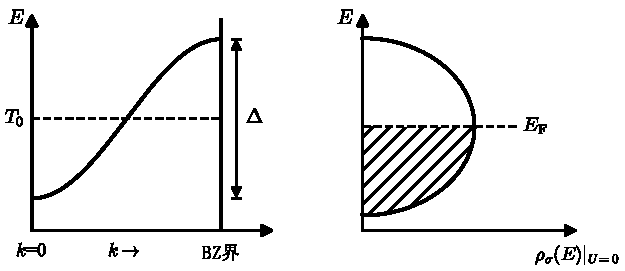
\includegraphics[width=9cm]{fig11-2.pdf}\\[0.3em]
{\small (a) 能带曲线\qquad\qquad (b) 态密度}\\[0.2em]
{\small 图 11.2\quad 不计关联时的单带示意图}
\end{minipage}
\end{center}

(ii) $U\geqslant\Delta$，即窄带中强关联情况.这时可设
\begin{equation}
  U\gg|E_{k}-T_{0}|
\end{equation}
再对式(11.1.53)和式(11.1.56)作展开，求得
\begin{equation}
\left.
\begin{aligned}
  &E^{(1)}_{k\sigma}\approx T_{0}+(E_{k}-T_{0})(1-\langle n_{\bar{\sigma}}\rangle)\\
  &E^{(2)}_{k\sigma}\approx U+T_{0}+(E_{k}-T_{0})\langle n_{\bar{\sigma}}\rangle
\end{aligned}\right\}
\end{equation}
\begin{equation}
  A^{(1)}_{k\sigma}\approx1-\langle n_{\bar{\sigma}}\rangle,
  \qquad A^{(2)}_{k\sigma}\approx\langle n_{\bar{\sigma}}\rangle
\end{equation}
格林函数和态密度的近似式为
\begin{equation}
  G^{\sigma}_{k}(\omega)\approx
  \biggl\{\frac{1-\langle n_{\bar{\sigma}}\rangle}
  {\omega-T_{0}-(E_{k}-T_{0})(1-\langle n_{\bar{\sigma}}\rangle)}
  +\frac{\langle n_{\bar{\sigma}}\rangle}
  {\omega-T_{0}-U-(E_{k}-T_{0})\langle n_{\bar{\sigma}}\rangle}\biggr\}
\end{equation}
\begin{equation}
  \rho_{\sigma}(\omega)\approx\frac{1}{N}\sum_{k}
  \bigl\{(1-\langle n_{\bar{\sigma}}\rangle)
  \delta\bigl[\omega-T_{0}-(E_{k}-T_{0})(1-\langle n_{\bar{\sigma}}\rangle)\bigr]
  +\langle n_{\bar{\sigma}}\rangle
  \delta\bigl[\omega-T_{0}-U-(E_{k}-T_{0})\langle n_{\bar{\sigma}}\rangle\bigr]\bigr\}
\end{equation}
显然，两个子带分别以 $T_{0}$ 和 $T_{0}+U$ 为中心.

对于零能带宽度情况，应取 $E_{k}=T_{0}$，这时式(11.1.64)还原为 $\Delta=0$ 情况的态密度公式(11.1.39)，而格林函数
\begin{equation}
  G^{\sigma}_{k}(\omega)\Big|_{\Delta=0}
  =\frac{1-\langle n_{\bar{\sigma}}\rangle}{\omega-T_{0}}
  +\frac{\langle n_{\bar{\sigma}}\rangle}{\omega-T_{0}-U}
\end{equation}
将上式代入表象变换式(11.1.47)，可求得格点格林函数
$G^{\sigma}_{ij}(\omega)=\delta_{ij}G^{\sigma}_{k}(\omega)\big|_{\Delta=0}$，
与孤立原子极限时的严格解［式(11.1.37)］相符.利用式(11.1.53)、(11.1.56)和(11.1.58)严格作出的能带曲线和态密度图形可参考赫伯德的原文\textsuperscript{[1]}.图11.3只是根据以上讨论所绘的示意图.

\begin{center}
\begin{minipage}{9cm}
\centering
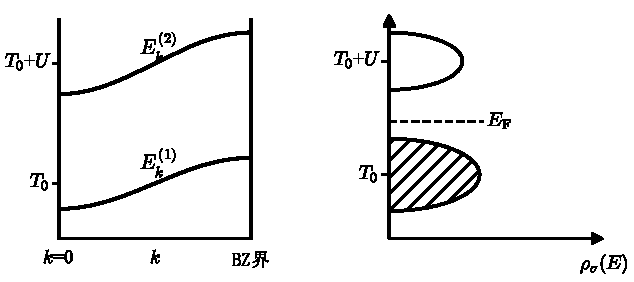
\includegraphics[width=9cm]{fig11-3.pdf}\\[0.3em]
{\small (a) 子能带曲线\qquad\qquad (b) 子带态密度的示意图}\\[0.2em]
{\small 图 11.3\quad 计入关联后的能带分裂图}
\end{minipage}
\end{center}

由以上图形可知，当 $E_{k}$ 能带为半满情况时，电子间的关联作用将使能带在费密能级 $E_{\mathrm{F}}$ 处发生分裂，从而形成两个子带，一个被填满另一个则是空带，将使金属变为绝缘体（称为M-I转变）.导致能带分裂的主要原因是同一格点周围的相反自旋电子间的库仑排斥作用，这是多体系统的强关联效应对能带的影响，可用于解释MnO及La$_{2}$CuO$_{4}$等化合物为什么是绝缘体.

\subsection*{5. 半满带中的金属-绝缘体转变}

以上讨论的一个结论是：只要计入了电子间的关联，则无论U多么小，都将导致单能带分裂为两个子带.事实上当 $U\ll\Delta$ 时这个结论是不正确的.因为从本节"3"的严格解可知，当不同格点上的原子局域轨道波函数不重叠时 $(\Delta=0)$，晶体中电子只可能处于 $T_{0}$ 和 $T_{0}+U$ 能级.当U很大而局域轨道重叠较小时 $(U\gg\Delta)$，各格点周围的 $T_{0}$ 和 $T_{0}+U$ 能级分别组成两个很窄的子能带，它们彼此不相交叠，对于 $n=1$ 情况（电子数$=$格点数），晶体仍为绝缘体.假如U较小而轨道波函数的重叠又很厉害，以至 $\Delta\gg U$，则以 $T_{0}$ 为中心和以 $T_{0}+U$ 为中心的两个子能带将彼此相交和重叠，实际上成为一个半填满的能带，这时晶体表现出金属性.因此，在半满能带 $E_{k}$ 中当计入电子关联作用后倒底是金属性的晶体(M)，还是绝缘体(I)取决于U和 $\Delta$ 的相对大小，在某个确定的比值 $(\Delta/U)_{\mathrm{c}}$ 处将发生M-I转变.

本节"4"中的理论之所以不能给出M-I转变的条件，是由于建立 $\Gamma^{\sigma}_{ij}(\omega)$ 的方程(11.1.43)时所采用的近似过于粗糙，忽略了子带的变宽效应.假如比(4)中处理更进一步，不对 $\Gamma^{\sigma}_{ij}(\omega)$ 方程作近似，而是写出严格的 $\Gamma^{\sigma}_{ij}(\omega)$ 方程.然后，再写出第三套格林函数锁链方程并对第三套方程作切断近似，使方程组封闭，则可以求得M-I转变的条件，这就是赫伯德后一个工作\textsuperscript{[3]}的要点.文献[3]中所求出的能带参量与 $(\Delta/U)$ 的关系如图11.4，当 $(\Delta/U)<\dfrac{2}{\sqrt{3}}$ 时半满带分裂为两个子带，系统表现出绝缘体特性.在相反的情况 $(\Delta/U)>\dfrac{2}{\sqrt{3}}$ 时，能带不分裂，晶体具有金属性.因此，$(\Delta/U)_{\mathrm{c}}=\dfrac{2}{\sqrt{3}}$ 是M-I转变点.这样用赫伯德模型就能够解释；同样是具有未填满d带的过渡金属氧化物，为什么有些是良导体，而另一些则是绝缘体.

\begin{center}
\begin{minipage}{6.5cm}
\centering
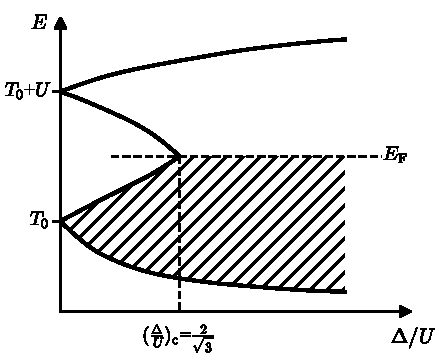
\includegraphics[width=6.5cm]{fig11-4.pdf}\\{\small 图 11.4\quad 赫伯德模型中的 M-I转变}
\end{minipage}
\end{center}

近年来赫伯德模型广泛用于强关联电子体系，发展了著名的t-J模型（见本章§9），用于建立铜氧化合物的高温超导理论（见本章§10）.此外，赫伯德模型还适用于讨论金属磁性问题，并在20世纪80年代初期发展了巡游电子磁性的自旋涨落理论，我们将在§11中作简要介绍.

\section{局域磁矩理论}

最简单的杂质局域态是半导体中的施主或受主能级状态，在第八章中我们曾经用有效哈密顿量讨论了这个问题.在那里杂质只是当作一个受到介质屏蔽的有心力势场处理，忽略了基质晶体中电子与杂质原子上电子之间的相互转移和状态混合效应.当基质晶体为金属、杂质是过渡族磁性原子时，状态的混合作用特别重要，它涉及金属中局域磁矩的形成问题，是局域态理论的一个重要方面.

大家知道，具有未填满d壳层的过渡元素，由于电子间的库仑排斥作用，d电子自旋矩按照洪德（Hund）定则排列，从而形成自由原子的固有磁矩.试问磁性原子溶入非磁性金属基体后是否仍保持原子的磁性状态？表11.1是局域磁矩的测量结果，表中还列出了基体金属的费密能 $E_{\mathrm{F}}$.

表 11.1\quad 金属基体中的杂质磁矩

{\small （"+"——有局域磁性，"$-$"——无局域磁矩，"？"——不明）}

\begin{center}\small
\begin{tabular}{lcccc}
\hline
磁性原子＼基体金属 & Au & Cu & Zn & Al\\
\hline
Mn & $+$ & $+$ & $+$ & $-$\\
Cr & $+$ & $+$ & $+$ & $-$\\
Fe & $+$ & $+$ & $-$ & $-$\\
Co & $?$ & $?$ & $?$ & $-$\\
Ni & $-$ & $-$ & $-$ & $-$\\
$E_{\mathrm{F}}$/eV & 5.5 & 7 & 9.5 & 13\\
\hline
\end{tabular}
\end{center}

显然，情况相当复杂，磁性原子溶入金属后并不都形成局域磁矩.例如，Fe溶于Cu中有局域磁矩，但Ni溶于Cu中就不产生局域磁性.又如，同样的磁性原子Mn在金属Cu中可测得局域磁矩，而在金属Al中室温下几乎测不出Mn的磁矩.因此，需要一个理论来说明在什么条件下金属中可形成局域磁矩？

\subsection*{1. 安德逊哈密顿量}

1961年安德逊\textsuperscript{[4]}提出了s-d混合模型（s-d mixing model），他认为在非磁性的金属基体中讨论过渡族杂质原子形成局域磁矩必须同时考虑两方面的因素：其一，和自由原子形成固有磁矩相似，杂质原子中d壳层电子的库仑作用对晶体形成局域磁矩有重要影响；其二，由于在晶体中杂质的自由原子d轨道状态 $\phi_{\mathrm{L}}(\boldsymbol{r})$ 不再是严格的本征态，特别是由于在金属晶体中存在着电子退局域化（delocalized）为布洛赫轨道态（s轨道）的倾向，$\phi_{\mathrm{L}}$ 与 $\phi_{k}$ 态之间存在着电子的相互转移，安德逊称之为s-d混合作用.为此，他指出系统的哈密顿量H应由下列四部分组成：

(i) 金属中能带电子的哈密顿量为
\begin{equation}
  \sum_{k,\,\sigma}E_{k}n_{k\sigma}
  \qquad(n_{k\sigma}=C^{+}_{k\sigma}C_{k\sigma})
\end{equation}
$E_{k}$ 代表布洛赫轨道电子能量，$C_{k\sigma}$ 是布洛赫表象中电子的消灭算符.

(ii) 杂质原子的未微扰d态哈密顿量为
\begin{equation}
  \sum_{\sigma}E_{\mathrm{d}}n_{\mathrm{d}}
  \qquad(n_{\mathrm{d}}=d^{+}_{\sigma}d_{\sigma})
\end{equation}
$d^{+}_{\sigma}$ 和 $d_{\sigma}$ 代表 $\phi_{\mathrm{L}}$ 轨道上 $\sigma$ 自旋的d电子的产生和消灭算符，$E_{\mathrm{d}}$ 是d态为单占据时的能量.即使是讨论孤立原子的磁矩形成问题，我们也必须考虑电子间的库仑关联作用，为简单起见设d态是非简并的，在反向自旋的d态电子之间有库仑排斥作用.因此

(iii) 关联作用项可写成
\begin{equation}
\begin{aligned}
  &Un_{\mathrm{d}\uparrow}n_{\mathrm{d}\downarrow}
  =\frac{U}{2}\sum_{\sigma}n_{\mathrm{d}\sigma}n_{\mathrm{d}\bar{\sigma}}\\
  &U=\int|\phi_{\mathrm{L}}(\boldsymbol{r})|^{2}
  |\phi_{\mathrm{L}}(\boldsymbol{r}')|^{2}
  \frac{e^{2}}{|\boldsymbol{r}-\boldsymbol{r}'|}
  \,\mathrm{d}\boldsymbol{r}\,\mathrm{d}\boldsymbol{r}'
\end{aligned}
\end{equation}
这里U是d电子的关联能.根据上节的讨论，如果 $E_{\mathrm{d}}$ 为第一个d电子的能量，则第二个自旋取向相反的电子在d态上的能量必为 $E_{\mathrm{d}}+U$，能量差U是形成磁矩的一个重要原因.但是，在金属中还存在 $\phi_{\mathrm{L}}$ 与 $\phi_{k}$ 态间的电子转移效应，其作用可表示为

(iv) s-d混合项
\begin{equation}
  \sum_{k,\,\sigma}V_{kd}
  \bigl(C^{+}_{k\sigma}d_{\sigma}+d^{+}_{\sigma}C_{k\sigma}\bigr)
\end{equation}
它代表布洛赫态与局域态之间的转移，是纯粹的单电子效应.$V_{kd}$ 称为s-d混合强度，来源于 $\phi_{\mathrm{L}}$ 与 $\phi_{k}$ 彼此不正交，可表示为
\begin{equation*}
\begin{aligned}
  V_{kd}&=\langle\phi_{\mathrm{L}}(\boldsymbol{r})|\mathscr{H}|\phi_{k}(\boldsymbol{r})\rangle\\
  &=\frac{1}{\sqrt{N}}\sum_{l}\mathrm{e}^{\mathrm{i}\boldsymbol{k}\cdot\boldsymbol{R}_{l}}
  \langle\phi_{\mathrm{L}}(\boldsymbol{r})|\mathscr{H}
  |a(\boldsymbol{r}-\boldsymbol{R}_{l})\rangle
\end{aligned}
\end{equation*}
其中杂质位于原点，$\mathscr{H}$ 是单电子哈密顿量，$a(\boldsymbol{r}-\boldsymbol{R}_{l})$ 是金属中能带电子的瓦尼尔函数.从第二个等式还可以看出，s-d混合作用与紧束缚近似中不同格点间电子的转移作用非常相似，其中 $\boldsymbol{R}_{l}=0$ 项对 $V_{kd}$ 无贡献，这是因为局域的d态函数 $\phi_{\mathrm{L}}(\boldsymbol{r})$ 与属于导带并以原点为中心的瓦尼尔函数 $a(\boldsymbol{r})$ 彼此是正交的.

综合以上四部分，再计入外加均匀磁场h的作用，得到总哈密顿量
\begin{equation}
\begin{aligned}
  H&=\sum_{k,\,\sigma}E_{k\sigma}n_{k\sigma}
  +\sum_{\sigma}E_{\mathrm{d}\sigma}n_{\mathrm{d}\sigma}
  +\frac{U}{2}\sum_{\sigma}n_{\mathrm{d}\sigma}n_{\mathrm{d}\bar{\sigma}}\\
  &\quad+\sum_{k,\,\sigma}V_{kd}
  \bigl(C^{+}_{k\sigma}d_{\sigma}+d^{+}_{\sigma}C_{k\sigma}\bigr)
\end{aligned}
\end{equation}
其中
\begin{equation}
  E_{k\sigma}=E_{k}+\sigma\mu_{\mathrm{B}}h,
  \qquad E_{\mathrm{d}\sigma}=E_{\mathrm{d}}+\sigma\mu_{\mathrm{B}}h
\end{equation}
这里 $\mu_{\mathrm{B}}=\dfrac{|e|\hbar}{2mc}$ 为玻尔磁子，并设电子与杂质的朗德（Landé）因子 $g_{0}=g_{i}=2$，这就是轨道非简并的安德逊s-d混合模型.

\subsection*{2. 安德逊s-d混合模型的格林函数}

从双时推迟格林函数
\begin{equation*}
  \langle\langle A(t);B(t')\rangle\rangle
  =-\mathrm{i}\theta(t-t')
  \langle[A(t),B(t')]_{+}\rangle
\end{equation*}
出发，利用一个技巧，对函数 $\langle\langle A(t);B(t')\rangle\rangle$ 分别求t及 $t'$ 的微商，可求得下列两个运动方程：
\begin{equation}
  \mathrm{i}\frac{\mathrm{d}}{\mathrm{d}t}
  \langle\langle A(t);B(t')\rangle\rangle
  =\delta(t-t')\langle[A,B]_{+}\rangle
  +\langle\langle[A,H];B(t')\rangle\rangle
\end{equation}
\begin{equation}
  -\mathrm{i}\frac{\mathrm{d}}{\mathrm{d}t'}
  \langle\langle A(t);B(t')\rangle\rangle
  =\delta(t-t')\langle[A,B]_{+}\rangle
  +\langle\langle A(t);[B,H]\rangle\rangle
\end{equation}
作傅里叶变换
\begin{equation}
  \langle\langle A\mid B\rangle\rangle_{\omega}
  =\int\mathrm{d}t\,\mathrm{e}^{\mathrm{i}\omega(t-t')}
  \langle\langle A(t);B(t')\rangle\rangle
\end{equation}
可得到格林函数运动方程通式的两种表示式
\begin{equation}
  \omega\langle\langle A\mid B\rangle\rangle_{\omega}
  =\langle[A,B]_{+}\rangle
  +\langle\langle[A,H]\mid B\rangle\rangle_{\omega}
\end{equation}
\begin{equation}
  \omega\langle\langle A\mid B\rangle\rangle_{\omega}
  =\langle[A,B]_{+}\rangle
  -\langle\langle A\mid[B,H]\rangle\rangle_{\omega}
\end{equation}
用它们处理s-d混合模型比较方便\textsuperscript{[5]}.

我们的目的是要找出形成局域磁矩的条件，即讨论系统在什么条件下有 $\langle n_{\mathrm{d}\uparrow}\rangle\neq\langle n_{\mathrm{d}\downarrow}\rangle$ 解？为此，应建立单粒子格林函数 $\langle\langle d_{\sigma}\mid d^{+}_{\sigma}\rangle\rangle_{\omega}$ 和 $\langle\langle C_{k\sigma}\mid C^{+}_{k\sigma}\rangle\rangle_{\omega}$ 的运动方程，利用式(11.2.10)写出
\begin{equation}
  (\omega-E_{k\sigma})
  \langle\langle C_{k\sigma}\mid C^{+}_{k'\sigma}\rangle\rangle_{\omega}
  =\delta_{k,\,k'}
  +V_{kd}\langle\langle d_{\sigma}\mid C^{+}_{k'\sigma}\rangle\rangle_{\omega}
\end{equation}
\begin{equation}
\begin{aligned}
  (\omega-E_{\mathrm{d}\sigma})
  \langle\langle d_{\sigma}\mid d^{+}_{\sigma}\rangle\rangle_{\omega}
  &=1+U\langle\langle n_{\mathrm{d}\bar{\sigma}}d_{\sigma}
  \mid d^{+}_{\sigma}\rangle\rangle_{\omega}\\
  &\quad+\sum_{k}V_{kd}
  \langle\langle C_{k\sigma}\mid d^{+}_{\sigma}\rangle\rangle_{\omega}
\end{aligned}
\end{equation}
对于混合格林函数 $\langle\langle C_{k\sigma}\mid d^{+}_{\sigma}\rangle\rangle_{\omega}$，仍通过式(11.2.10)写运动方程
\begin{equation}
  (\omega-E_{k\sigma})
  \langle\langle C_{k\sigma}\mid d^{+}_{\sigma}\rangle\rangle_{\omega}
  =V_{kd}\langle\langle d_{\sigma}\mid d^{+}_{\sigma}\rangle\rangle_{\omega}
\end{equation}
另一个混合格林函数 $\langle\langle d_{\sigma}\mid C^{+}_{k\sigma}\rangle\rangle_{\omega}$ 则利用第二套运动方程的通式(11.2.11)，求得
\begin{equation}
  (\omega-E_{k'\sigma})
  \langle\langle d_{\sigma}\mid C^{+}_{k'\sigma}\rangle\rangle_{\omega}
  =V_{k'd}\langle\langle d_{\sigma}\mid d^{+}_{\sigma}\rangle\rangle_{\omega}
\end{equation}
如果对方程(11.2.13)中的高阶格林函数作切断近似：
\begin{equation}
  \langle\langle n_{\mathrm{d}\bar{\sigma}}d_{\sigma}\mid d^{+}_{\sigma}\rangle\rangle_{\omega}
  \approx\langle n_{\mathrm{d}\bar{\sigma}}\rangle
  \langle\langle d_{\sigma}\mid d^{+}_{\sigma}\rangle\rangle_{\omega}
\end{equation}
将得到近似式
\begin{equation}
  (\omega-E_{\mathrm{d}\sigma}-U\langle n_{\mathrm{d}\bar{\sigma}}\rangle)
  \langle\langle d_{\sigma}\mid d^{+}_{\sigma}\rangle\rangle_{\omega}
  =1+\sum_{k}V_{kd}
  \langle\langle C_{k\sigma}\mid d^{+}_{\sigma}\rangle\rangle_{\omega}
\end{equation}
这时式(11.2.12)、式(11.2.14)、式(11.2.15)和(11.2.17)构成近似封闭的格林函数方程组，格林函数可解出.切断近似式(11.2.16)相当于对H中的关联项作下列线性化近似：
\begin{equation}
  \frac{U}{2}\sum_{\sigma}n_{\mathrm{d}\sigma}n_{\mathrm{d}\bar{\sigma}}
  \approx U\sum_{\sigma}\langle n_{\mathrm{d}\bar{\sigma}}\rangle n_{\mathrm{d}\sigma}
  -U\langle n_{\mathrm{d}\uparrow}\rangle\langle n_{\mathrm{d}\downarrow}\rangle
\end{equation}
显然这就是哈特利-福克近似.因此，用上述切断近似所建立的格林函数封闭方程组属于哈特利-福克近似(HFA).

现在求格林函数的HFA解.将式(11.2.15)代入式(11.2.12)，求得
\begin{equation}
  \langle\langle C_{k\sigma}\mid C^{+}_{k'\sigma}\rangle\rangle_{\omega}
  =\frac{\delta_{kk'}}{(\omega-E_{k\sigma})}
  +\frac{V_{kd}V_{k'd}}{(\omega-E_{k\sigma})(\omega-E_{k'\sigma})}
  \langle\langle d_{\sigma}\mid d^{+}_{\sigma}\rangle\rangle_{\omega}
\end{equation}
其中等式右边第一项为自由粒子的格林函数，第二项代表s-d混合作用的影响.格林函数 $\langle\langle d_{\sigma}\mid d^{+}_{\sigma}\rangle\rangle_{\omega}$ 由式(11.2.14)代入近似式(11.2.17)，消去 $\langle\langle C_{k\sigma}\mid d^{+}_{\sigma}\rangle\rangle_{\omega}$ 后为
\begin{equation}
  \langle\langle d_{\sigma}\mid d^{+}_{\sigma}\rangle\rangle_{\omega}
  =\frac{1}{\omega-E_{\mathrm{d}\sigma}
  -U\langle n_{\mathrm{d}\bar{\sigma}}\rangle-F_{\sigma}(\omega)}
\end{equation}
对于推迟格林函数应取 $\omega+\mathrm{i}\eta$.在上式中
\begin{equation}
\begin{aligned}
  F_{\sigma}(\omega+\mathrm{i}\eta)
  &=\sum_{k}\frac{V^{2}_{k\sigma}}{(\omega-E_{k\sigma}+\mathrm{i}\eta)}
  \qquad(\eta=+0)\\
  &=\mathscr{P}\int\frac{\rho^{(0)}(E)}{\omega-E}V^{2}_{kd}\,\mathrm{d}E
  -\mathrm{i}\pi V^{2}_{kd}\rho^{(0)}(\omega)\\
  &\approx-\mathrm{i}\pi V^{2}_{kd}\rho^{(0)}(\omega)
\end{aligned}
\end{equation}
$\rho^{(0)}(E)$ 是能带电子的态密度，可近似取其费密面上值 $\rho^{(0)}_{\mathrm{F}}$，而主值积分 $\mathscr{P}\int(\cdots)\,\mathrm{d}E$ 项的贡献很小，可以略去（或归并到 $E_{\mathrm{d}\sigma}$ 中）.定义常数
\begin{equation}
  \Gamma\equiv\pi V^{2}_{kd}\rho^{(0)}_{\mathrm{F}}
\end{equation}
将d电子格林函数的哈特利-福克近似解写成
\begin{equation}
  \langle\langle d_{\sigma}\mid d^{+}_{\sigma}\rangle\rangle_{\omega+\mathrm{i}\eta}
  =\frac{1}{\omega-E_{\mathrm{d}\sigma}
  -U\langle n_{\mathrm{d}\bar{\sigma}}\rangle+\mathrm{i}\Gamma}
\end{equation}
\begin{equation}
  \langle\langle d_{\sigma}\mid d^{+}_{\sigma}\rangle\rangle_{\omega-\mathrm{i}\eta}
  =\frac{1}{\omega-E_{\mathrm{d}\sigma}
  -U\langle n_{\mathrm{d}\bar{\sigma}}\rangle-\mathrm{i}\Gamma}
\end{equation}
再把它们代入式(11.2.19)，即可求出布洛赫电子的格林函数近似解.式(11.2.23)表明，d电子推迟格林函数的极点在复平面上 $(E_{\mathrm{d}\sigma}+U\langle n_{\mathrm{d}\bar{\sigma}}\rangle)-\mathrm{i}\Gamma$ 处，$\Gamma$ 与s-d混合作用强度有关.在这里库仑作用改变极点之实部，使能级移动，而s-d混合则使极点离开实轴，导致d电子的有限寿命 $\Gamma^{-1}$.因为对d电子的推迟格林函数式(11.2.23)作傅里叶变换，类似于附录D中式(D.22)，可写出含时的d电子推迟格林函数
\begin{equation*}
\begin{aligned}
  G_{\mathrm{r}}(t)&=\frac{1}{2\pi}\int_{-\infty}^{\infty}\mathrm{d}\omega\,
  \frac{\mathrm{e}^{-\mathrm{i}\omega t}}{\omega-\tilde{E}_{\mathrm{d}\sigma}+\mathrm{i}\Gamma}\\
  &=-\mathrm{i}\theta(t)\mathrm{e}^{-\mathrm{i}\tilde{E}_{\mathrm{d}\sigma}t}
  \mathrm{e}^{-\Gamma t}
\end{aligned}
\end{equation*}
其中
\begin{equation*}
  \tilde{E}_{\mathrm{d}\sigma}\equiv E_{\mathrm{d}\sigma}
  +U\langle n_{\mathrm{d}\bar{\sigma}}\rangle
\end{equation*}
显然，d电子在传播过程中将衰减，其寿命正比于 $\Gamma^{-1}$.

\subsection*{3. 静态磁化率}

系统的静态磁化率应包括布洛赫能带态电子和局域态d电子的贡献.因此
\begin{equation}
  \chi=\lim_{h\to0}\biggl\{\sum_{k}
  \bigl(\langle C^{+}_{k\downarrow}C_{k\downarrow}\rangle
  -\langle C^{+}_{k\uparrow}C_{k\uparrow}\rangle\bigr)\frac{\mu_{\mathrm{B}}}{h}
  +\bigl(\langle d^{+}_{\downarrow}d_{\downarrow}\rangle
  -\langle d^{+}_{\uparrow}d_{\uparrow}\rangle\bigr)\frac{\mu_{\mathrm{B}}}{h}\biggr\}
\end{equation}
其中平均量 $\langle BA\rangle$ 由谱定理决定，记为 $\mathscr{F}_{\omega}(\langle\langle A\mid B\rangle\rangle_{\omega})$
\begin{equation}
\begin{aligned}
  \langle\,BA\,\rangle&=\frac{\mathrm{i}}{2\pi}\int_{-\infty}^{\infty}
  \bigl\{\langle\langle A\mid B\rangle\rangle_{\omega+\mathrm{i}\eta}
  -\langle\langle A\mid B\rangle\rangle_{\omega-\mathrm{i}\eta}\bigr\}
  f(\omega)\,\mathrm{d}\omega\\
  &\equiv\mathscr{F}_{\omega}(\langle\langle A\mid B\rangle\rangle_{\omega})
\end{aligned}
\end{equation}
根据式(11.2.19)，磁化率可写成
\begin{equation}
  \chi=\chi_{\mathrm{p}}+\lim_{h\to0}\sum_{\sigma=\pm1}\frac{\sigma\mu_{\mathrm{B}}}{h}
  \biggl\{\sum_{k}\mathscr{F}_{\omega}\biggl[\frac{V^{2}_{kd}}{(\omega-E_{k\sigma})^{2}}
  \langle\langle d_{\sigma}\mid d^{+}_{\sigma}\rangle\rangle_{\omega}\biggr]
  +\mathscr{F}_{\omega}\bigl[\langle\langle d_{\sigma}\mid d^{+}_{\sigma}\rangle\rangle_{\omega}\bigr]\biggr\}
\end{equation}
上式中 $\chi_{\mathrm{p}}$ 项代表式(11.2.19)中自由粒子格林函数的贡献，读者不难证明它就是自由电子的泡利磁化率.式(11.2.27)中第一个 $\mathscr{F}_{\omega}$ 项的贡献可证明为零.这是因为对 $\omega$ 积分与对k求和可对调，于是在 $\omega$ 积分中有下列被积函数因子：
\begin{equation*}
  \sum_{k}\frac{V^{2}_{kd}}{(\omega-E_{k\sigma}\pm\mathrm{i}\eta)^{2}}
  =\int_{-\infty}^{\infty}
  \frac{\rho^{(0)}(E)|V_{kd}|^{2}}{(\omega-E\pm\mathrm{i}\eta)^{2}}\,\mathrm{d}E
\end{equation*}
若将 $\rho^{(0)}(E)$ 和 $|V_{kd}|^{2}$ 近似当作与E无关的常数，则这个积分的贡献为零.因此式(11.2.27)中第二项可略去.这样，除泡利磁化率外，只需再计算d电子对磁化率的贡献.将d电子的格林函数解式(11.2.23)和式(11.2.24)代入谱定理公式(11.2.26)，得
\begin{equation}
\begin{aligned}
  \mathscr{F}_{\omega}\bigl[\langle\langle d_{\sigma}\mid d^{+}_{\sigma}\rangle\rangle_{\omega}\bigr]
  &=\langle d^{+}_{\sigma}d_{\sigma}\rangle
  =\langle n_{\mathrm{d}\sigma}\rangle\\
  &=\frac{1}{\pi}\int_{-\infty}^{\infty}\mathrm{d}\omega\,f(\omega)
  \biggl\{\frac{\Gamma}{(\omega-\tilde{E}_{\mathrm{d}\sigma})^{2}+\Gamma^{2}}\biggr\}\\
  &\equiv\int_{-\infty}^{\infty}\mathrm{d}\omega\,f(\omega)\rho_{\mathrm{d}\sigma}(\omega)
\end{aligned}
\end{equation}
其中 $\rho_{\mathrm{d}\sigma}(\omega)$ 代表 $\sigma$ 自旋的d电子的态密度
\begin{equation}
  \rho_{\mathrm{d}\sigma}(\omega)=\frac{1}{\pi}
  \frac{\Gamma}{(\omega-\tilde{E}_{\mathrm{d}\sigma})^{2}+\Gamma^{2}}
\end{equation}
这里
\begin{equation}
  \tilde{E}_{\mathrm{d}\sigma}=E_{\mathrm{d}}+\sigma\mu_{\mathrm{B}}h
  +U\langle n_{\mathrm{d}\bar{\sigma}}\rangle
\end{equation}
由图11.5可知，$\rho_{\mathrm{d}\sigma}$ 是半宽度为 $\Gamma$ 的共振峰，峰的中心在 $\tilde{E}_{\mathrm{d}\sigma}$ 处，称为洛仑兹型（Lorentzian）态密度.这时金属中d电子不再是具有确定能级并且态密度为 $\delta$ 函数的束缚态，而是能级分布在 $\tilde{E}_{\mathrm{d}\sigma}$ 周围 $2\Gamma$ 宽度内的共振态（resonance state），由于它仍具有局域特性，有时也称之为虚束缚态（virtual bound state）.

\begin{center}
\begin{minipage}{4.5cm}
\centering
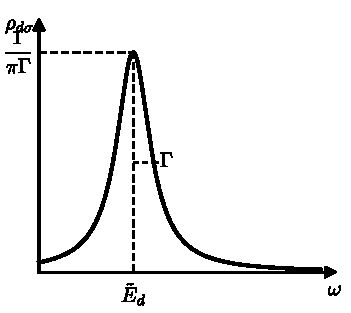
\includegraphics[width=4.5cm]{fig11-5.pdf}\\{\small 图 11.5\quad 局域电子态密度}
\end{minipage}
\end{center}

利用态密度可以计算 $T=0$ K时d态上的平均占据数.由于零温费密分布为
\begin{equation}
  f(\omega)=\begin{cases}1&(E<E_{\mathrm{F}})\\0&(E>E_{\mathrm{F}})\end{cases}
\end{equation}
代入式(11.2.28)，求得
\begin{equation}
  \langle n_{\mathrm{d}\sigma}\rangle
  =\int_{-\infty}^{E_{\mathrm{F}}}\rho_{\mathrm{d}\sigma}(\omega)\,\mathrm{d}\omega
  =\frac{1}{\pi}\mathrm{arccot}
  \biggl(\frac{\tilde{E}_{\mathrm{d}\sigma}-E_{\mathrm{F}}}{\Gamma}\biggr)
\end{equation}
式(11.2.32)实际上是自洽方程组
\begin{equation}
\left.
\begin{aligned}
  \langle n_{\mathrm{d}\uparrow}\rangle
  &=\frac{1}{\pi}\mathrm{arccot}
  \biggl[\frac{E_{\mathrm{d}}-E_{\mathrm{F}}
  +U\langle n_{\mathrm{d}\downarrow}\rangle+\mu_{\mathrm{B}}h}{\Gamma}\biggr]\\
  \langle n_{\mathrm{d}\downarrow}\rangle
  &=\frac{1}{\pi}\mathrm{arccot}
  \biggl[\frac{E_{\mathrm{d}}-E_{\mathrm{F}}
  +U\langle n_{\mathrm{d}\uparrow}\rangle-\mu_{\mathrm{B}}h}{\Gamma}\biggr]
\end{aligned}\right\}
\end{equation}
当 $h=0$ 时，如果求得 $\langle n_{\mathrm{d}\uparrow}\rangle\neq\langle n_{\mathrm{d}\downarrow}\rangle$ 解，就说明有局域磁矩，而 $\langle n_{\mathrm{d}\uparrow}\rangle=\langle n_{\mathrm{d}\downarrow}\rangle$ 解则代表无局域磁矩情况.但是，从式(11.2.33)往往同时求得有磁矩与无磁矩两种解.这时还需要一个判据确定那种解是稳定的.最简单的办法是从系统的顺磁磁化率来作判断.为此讨论杂质的非磁情况，考虑外磁场 $h=0$ 时，式(11.2.33)有非磁解
\begin{equation}
  \langle n_{\mathrm{d}\uparrow}\rangle
  =\langle n_{\mathrm{d}\downarrow}\rangle=n_{0}
\end{equation}
则在弱磁场作用时可设
\begin{equation}
\left.
\begin{aligned}
  &\langle n_{\mathrm{d}\uparrow}\rangle=n_{0}-h\Delta\\
  &\langle n_{\mathrm{d}\downarrow}\rangle=n_{0}+h\Delta
\end{aligned}\right\}
\end{equation}
外场产生的磁化正比于
\begin{equation}
  \langle n_{\mathrm{d}\downarrow}\rangle
  -\langle n_{\mathrm{d}\uparrow}\rangle=2h\Delta
\end{equation}
将式(11.2.33)对h作展开，并利用式(11.2.29)和式(11.2.36)定出未知量
\begin{equation}
  \Delta=\mu_{\mathrm{B}}
  \frac{\rho_{\mathrm{d}\sigma}(E_{\mathrm{F}})}
  {1-U\rho_{\mathrm{d}\sigma}(E_{\mathrm{F}})}
\end{equation}
根据式(11.2.27)，系统的顺磁磁化率为
\begin{equation*}
  \chi=\chi_{\mathrm{P}}+\chi_{\mathrm{I}}
\end{equation*}
$\chi_{\mathrm{I}}$ 代表杂质上d电子的磁化率，大小为
\begin{equation}
\begin{aligned}
  \chi_{\mathrm{I}}
  &=\lim_{h\to0}\bigl(\langle n_{\mathrm{d}\downarrow}\rangle
  -\langle n_{\mathrm{d}\uparrow}\rangle\bigr)\frac{\mu_{\mathrm{B}}}{h}\\
  &=2\mu^{2}_{\mathrm{B}}
  \frac{\rho_{\mathrm{d}\sigma}(E_{\mathrm{F}})}
  {1-U\rho_{\mathrm{d}\sigma}(E_{\mathrm{F}})}
\end{aligned}
\end{equation}
其中 $\rho_{\mathrm{d}\sigma}(E_{\mathrm{F}})$ 是 $\langle n_{\mathrm{d}\uparrow}\rangle=\langle n_{\mathrm{d}\downarrow}\rangle=n_{0}$ 情况下的d电子态密度，写为
\begin{equation}
\begin{aligned}
  \rho_{\mathrm{d}\sigma}(E_{\mathrm{F}})
  &=\frac{1}{\pi}
  \frac{\Gamma}{(E_{\mathrm{d}}+Un_{0}-E_{\mathrm{F}})^{2}+\Gamma^{2}}\\
  &=\frac{1}{\pi}\frac{1}{\Gamma[1+\cot^{2}(\pi n_{0})]}
  =\frac{1}{\pi}\frac{\sin^{2}\pi n_{0}}{\Gamma}
\end{aligned}
\end{equation}
在这里利用了公式
\begin{equation}
  n_{0}=\frac{1}{\pi}\mathrm{arccot}
  \biggl[\frac{E_{\mathrm{d}}+Un_{0}-E_{\mathrm{F}}}{\Gamma}\biggr]
\end{equation}
它代表无外场时式(11.2.33)有 $\langle n_{\mathrm{d}\uparrow}\rangle=\langle n_{\mathrm{d}\downarrow}\rangle$ 非磁解的情况.

由于 $T=0$ K时泡利磁化率为常数，并且它与U和 $\Gamma$ 无关.杂质磁化率 $\chi_{\mathrm{I}}$ 根据式(11.2.38)和(11.2.39)可写成
\begin{equation}
  \chi_{\mathrm{I}}=2\mu^{2}_{\mathrm{B}}
  \frac{\rho_{\mathrm{d}\sigma}(E_{\mathrm{F}})}
  {1-U\rho_{\mathrm{d}\sigma}(E_{\mathrm{F}})}
  =2\mu^{2}_{\mathrm{B}}
  \frac{1}{\biggl[\dfrac{\pi\Gamma}{\sin^{2}n_{0}\pi}-U\biggr]}
\end{equation}
上式仅仅在 $U\rho_{\mathrm{d}\sigma}(E_{\mathrm{F}})<1$ 时成立，这时 $\chi_{\mathrm{I}}>0$，对应于自由能极小，因此非磁解是稳定的，反过来当 $U\rho_{\mathrm{d}\sigma}(E_{\mathrm{F}})>1$ 时，非磁解
$\langle n_{\mathrm{d}\uparrow}\rangle_{h=0}
=\langle n_{\mathrm{d}\downarrow}\rangle_{h=0}$
不再是稳定的.由此推论，当 $U\rho_{\mathrm{d}\sigma}(E_{\mathrm{F}})>1$ 时，只可能有
$\langle n_{\mathrm{d}\uparrow}\rangle_{h=0}
\neq\langle n_{\mathrm{d}\downarrow}\rangle_{h=0}$
的磁性解.磁化率 $\chi_{\mathrm{I}}$ 的发散点出现在
\begin{equation}
  U\rho_{\mathrm{d}\sigma}(E_{\mathrm{F}})=1
  \quad\text{或}\quad
  U=\frac{\pi\Gamma}{\sin^{2}\pi n_{0}}
\end{equation}
处，它代表金属中杂质的非磁性与磁性状态的转变边界.

\subsection*{4. 局域磁矩的存在}

为了证实以上推论，我们现在讨论 $h=0$ 时自洽方程式(11.2.33)的磁性及非磁解.将式(11.2.33)的两个方程改写为下列形式：
\begin{equation}
  \langle n_{\mathrm{d}\uparrow}\rangle
  =\frac{\Gamma}{U}\cot\bigl[\pi\langle n_{\mathrm{d}\downarrow}\rangle\bigr]
  +\frac{E_{\mathrm{F}}-E_{\mathrm{d}}}{U}
\end{equation}
\begin{equation}
  \langle n_{\mathrm{d}\downarrow}\rangle
  =\frac{\Gamma}{U}\cot\bigl[\pi\langle n_{\mathrm{d}\uparrow}\rangle\bigr]
  +\frac{E_{\mathrm{F}}-E_{\mathrm{d}}}{U}
\end{equation}
并利用作图法求解.具体步骤：对给定的参数值 $\Gamma/U$ 和 $(E_{\mathrm{F}}-E_{\mathrm{d}})/U$，分别由式(11.2.43)和式(11.2.44)作 $\langle n_{\mathrm{d}\uparrow}\rangle$ 随 $\langle n_{\mathrm{d}\downarrow}\rangle$ 的变化曲线，两曲线的交点代表自洽方程的解.图11.6(a)和(b)为参数取下列值的解：
\begin{equation}
  E_{\mathrm{F}}-E_{\mathrm{d}}=\frac{U}{2}
  \quad\text{和}\quad
  \frac{\Gamma}{U}=
  \begin{cases}1&\text{(a)}\\[0.3em] \dfrac{1}{5}&\text{(b)}\end{cases}
\end{equation}
显然，在情况(a)只有非磁解
\begin{equation*}
  \langle n_{\mathrm{d}\uparrow}\rangle
  =\langle n_{\mathrm{d}\downarrow}\rangle
  =\frac{1}{2}=n_{0}
\end{equation*}
这时根据式(11.2.39)，$\rho_{\mathrm{d}\sigma}(E_{\mathrm{F}})=(\pi\Gamma)^{-1}$，因此
\begin{equation}
  U\rho_{\mathrm{d}\sigma}(E_{\mathrm{F}})
  =\frac{U}{\pi\Gamma}=\frac{1}{\pi}<1
\end{equation}
非磁解 $n_{0}=\dfrac{1}{2}$ 是稳定的，杂质不表现局域磁性.

对于情况(b)，除了图(b)中A点代表非磁解外，在 $0<\langle n_{\mathrm{d}\sigma}\rangle<1$ 区域内还有两个对称并且等效的磁性解，如图11.6(b)中两边的黑点所示.根据式(11.2.41)和式(11.2.42)的讨论可知，这时A点所代表的非磁解是不稳定的，因为在(b)情况下非磁解的
\begin{equation}
  U\rho_{\mathrm{d}\sigma}(E_{\mathrm{F}})
  =\frac{U}{\pi\Gamma}=\frac{5}{\pi}>1
\end{equation}
这样就证实了"3"中的推论；当 $U\rho_{\mathrm{d}\sigma}(E_{\mathrm{F}})<1$ 时金属中杂质只有非磁解，不形成局域磁矩.而当 $U\rho_{\mathrm{d}\sigma}(E_{\mathrm{F}})>1$ 时，稳定解是磁性的，金属中杂质呈现局域磁矩(LM).因此，
\begin{equation*}
  U\rho_{\mathrm{d}\sigma}(E_{\mathrm{F}})=1
\end{equation*}
代表磁和非磁的转变曲线，图11.7是根据式(11.2.42)所作的边界，形成局域磁矩要求 $x\equiv(E_{\mathrm{F}}-E_{\mathrm{d}})/U$ 介于0到1之间.显然，在基体Al中均不形成局域磁矩的原因是由于 $E_{\mathrm{F}}$ 值过大，甚至超过了 $(E_{\mathrm{d}}+U)$，导致磁杂质在Al基体中只可能形成无局域磁矩的双占据态.

\begin{center}
\begin{minipage}{9.5cm}
\centering
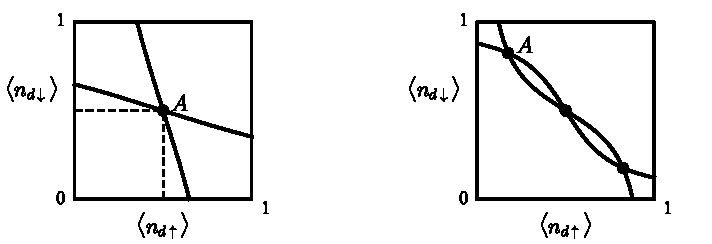
\includegraphics[width=9.5cm]{fig11-6.pdf}\\[0.3em]
{\small (a) $U=\Gamma$，$E_{\mathrm{F}}-E_{\mathrm{d}}=\dfrac{U}{2}$，
$\langle n_{\mathrm{d}\downarrow}\rangle=\langle n_{\mathrm{d}\uparrow}\rangle=\dfrac{1}{2}$
\qquad
(b) $U=5\Gamma$，$E_{\mathrm{F}}-E_{\mathrm{d}}=\dfrac{U}{2}$，
$\langle n_{\mathrm{d}\downarrow}\rangle\neq\langle n_{\mathrm{d}\uparrow}\rangle$}\\[0.2em]
{\small 图 11.6\quad $\langle n_{\mathrm{d}\sigma}\rangle$ 的自洽解}
\end{minipage}
\end{center}

\begin{center}
\begin{minipage}{6cm}
\centering
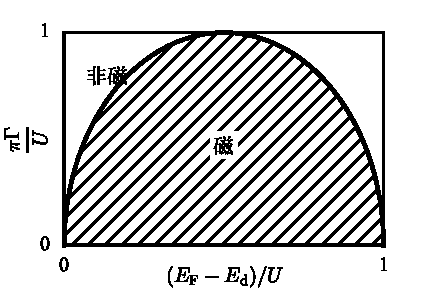
\includegraphics[width=6cm]{fig11-7.pdf}\\{\small 图 11.7\quad 安德逊哈特利-福克解的磁性与非磁性区域}
\end{minipage}
\end{center}

综上所述，安德逊模型的哈特利-福克近似解能够说明非磁性金属基体中杂质磁矩的形成条件.当费密能级 $E_{\mathrm{F}}$ 位于 $E_{\mathrm{d}}$ 和 $E_{\mathrm{d}}+U$ 的中间、并且d电子态密度的半峰宽 $\Gamma\ll U$ 时，将是形成局域磁矩的最有利条件.稀土元素的杂质（其 $U\approx15$ eV，$\Gamma\leqslant1$ eV）往往满足最有利条件，因此它们多数在金属中形成局域磁矩.由于铁族过渡元素的 $U\approx10$ eV，$\Gamma\approx2\sim5$ eV，其 $\pi\Gamma$ 值，对于不同的铁族元素，可能小于或大于U，而磁与非磁解的转变边界大约在 $\pi\Gamma/U=1$ 处.按此估计，当铁族杂质溶于金属中时有些产生局域磁矩，另一些则只能形成非磁性的局域态.在具体说明各种杂质的局域磁矩时，还需要考虑d能级简并问题，特别是各简并轨道间交换作用对边界的修正，这方面的工作可参阅文献[6].近年来安德逊模型已推广到每个元胞中均含一个磁性原子的情况，此即周期性安德逊模型（又称安德逊晶格模型，简称ALM），它用于说明稀土金属及其化合物的变价特性\textsuperscript{[7]}和重费密子特征.我们将在§7中引入ALM，并在§8中介绍此模型对重费密子系统的应用.

\section{s-d交换模型}

如果杂质原子在金属中已形成局域磁矩，它对金属中电子的输运特性有何影响？要回答这个问题必须首先讨论金属中局域磁矩与传导电子之间的相互作用.

设金属中含有少量磁性杂质原子，并都已形成磁矩，在 $\boldsymbol{R}_{n}$ 格点上杂质的自旋矩由算符 $\hat{\boldsymbol{S}}_{n}$ 描述，它代表杂质d壳层局域电子的总自旋算符.从多体理论可以证明传导电子(s)与形成磁矩的局域电子(d)之间的交换作用为
\begin{equation}
\begin{aligned}
  \mathscr{H}_{\mathrm{s}\text{-}\mathrm{d}}
  &=-\frac{J}{N}\sum_{n}\sum_{k,\,k'}
  \mathrm{e}^{\mathrm{i}(\boldsymbol{k}'-\boldsymbol{k})\cdot\boldsymbol{R}_{n}}
  \bigl\{\bigl(C^{+}_{k\uparrow}C_{k'\uparrow}
  -C^{+}_{k\downarrow}C_{k'\downarrow}\bigr)\hat{S}^{z}_{n}\\
  &\qquad+C^{+}_{k\uparrow}C_{k'\downarrow}\hat{S}^{-}_{n}
  +C^{+}_{k\downarrow}C_{k'\uparrow}\hat{S}^{+}_{n}\bigr\}
\end{aligned}
\end{equation}
称为s-d交换作用，其中J为交换积分，N代表原子数，$C^{+}_{k\sigma}$ 与 $C_{k\sigma}$（$\sigma=\uparrow,\,\downarrow$）是传导电子的产生和消灭算符，$\boldsymbol{k}$ 为波矢.式(11.3.1)就是局域磁矩与传导电子相互作用哈密顿量.

我们将介绍糟谷（Kasuya）的简单证明\textsuperscript{[8]}，讨论杂质自旋 $S_{n}=\dfrac{1}{2}$ 情况.由于存在杂质磁矩，应要求d态满足单占条件
\begin{equation}
  C^{+}_{n\uparrow}C_{n\uparrow}+C^{+}_{n\downarrow}C_{n\downarrow}=1
\end{equation}
这时d电子要么占据自旋朝上态，要么自旋朝下，从而保证 $S_{n}=\dfrac{1}{2}$.$C^{+}_{n\sigma}$ 与 $C_{n\sigma}$ 是局域电子(d)的产生及消灭算符.根据式(3.2.16)，$\hat{\boldsymbol{S}}_{n}$ 与 $C^{+}_{n\sigma}$、$C_{n\sigma}$ 的关系为
\begin{equation}
\left.
\begin{aligned}
  &\frac{1}{2}\bigl(C^{+}_{n\uparrow}C_{n\uparrow}
  -C^{+}_{n\downarrow}C_{n\downarrow}\bigr)=\hat{S}^{z}_{n}\\
  &C^{+}_{n\uparrow}C_{n\downarrow}=\hat{S}^{+}_{n}\\
  &C^{+}_{n\downarrow}C_{n\uparrow}=\hat{S}^{-}_{n}
\end{aligned}\right\}
\end{equation}
设 $\phi_{k}(\boldsymbol{r})$ 为传导电子(s)的布洛赫函数，$\phi_{\mathrm{L}}(\boldsymbol{r}-\boldsymbol{R}_{n})$ 代表以 $\boldsymbol{R}_{n}$ 格点为中心的局域d电子波函数，则s电子与d电子系统的二次量子化态矢量可写成
\begin{equation}
  \varPsi(\boldsymbol{r},\zeta)
  =\sum_{k,\,\sigma}C_{k\sigma}\phi_{k}(\boldsymbol{r})\chi_{\sigma}(\zeta)
  +\sum_{n,\,\sigma}C_{n\sigma}
  \phi_{\mathrm{L}}(\boldsymbol{r}-\boldsymbol{R}_{n})\chi_{\sigma}(\zeta)
\end{equation}
其中 $\chi_{\sigma}(\zeta)$ 为单电子的自旋函数，$\zeta$ 为自旋坐标，并满足条件：
\begin{equation}
  \int\chi^{+}_{\sigma}(\zeta)\chi_{\sigma'}(\zeta)\,\mathrm{d}\zeta
  =\delta_{\sigma\sigma'}
\end{equation}
系统的电子-电子相互作用可表示为
\begin{equation}
  \frac{1}{2}\int\cdots\int
  \varPsi^{+}(\boldsymbol{r}_{1},\zeta_{1})
  \varPsi^{+}(\boldsymbol{r}_{2},\zeta_{2})
  v(\boldsymbol{r}_{12})
  \varPsi(\boldsymbol{r}_{2},\zeta_{2})
  \varPsi(\boldsymbol{r}_{1},\zeta_{1})
  \,\mathrm{d}\boldsymbol{r}_{1}\,\mathrm{d}\boldsymbol{r}_{2}
  \,\mathrm{d}\zeta_{1}\,\mathrm{d}\zeta_{2}
\end{equation}
这里 $v(\boldsymbol{r}_{12})$ 为电子间的二体互作用势，而
\begin{equation}
  \boldsymbol{r}_{12}=\boldsymbol{r}_{1}-\boldsymbol{r}_{2}
\end{equation}
当式(11.3.4)代入式(11.3.6)后，将得到很多项.我们仅取其中含算符
$C^{+}_{k\sigma}C_{k'\sigma'}C^{+}_{n\sigma''}C_{n\sigma'''}$
的项 $\mathscr{H}_{i}$，它代表传导电子不改变局域电子位置的散射项.这样做才能代表传导电子与局域自旋的互作用.再考虑到互作用势 $v(\boldsymbol{r}_{12})$ 与自旋无关，这项作用应满足总自旋守恒条件，得到
\begin{equation}
\begin{aligned}
  \mathscr{H}_{i}&=\sum_{n}\sum_{k,\,k'}\sum_{\sigma,\,\sigma'}
  \bigl\{C^{+}_{k\sigma}C_{k'\sigma}C^{+}_{n\sigma'}C_{n\sigma'}
  \langle\,kn\mid v\mid k'n\,\rangle\\
  &\quad-C^{+}_{k\sigma}C_{k'\sigma'}C^{+}_{n\sigma'}C_{n\sigma}
  \langle\,kn\mid v\mid nk'\,\rangle\bigr\}
\end{aligned}
\end{equation}
这里
\begin{equation}
\begin{aligned}
  \langle\,kn\mid v\mid k'n\,\rangle
  &=\int\phi^{*}_{k}(\boldsymbol{r}_{1})
  \phi^{*}_{\mathrm{L}}(\boldsymbol{r}_{2}-\boldsymbol{R}_{n})
  v(\boldsymbol{r}_{12})\\
  &\qquad\times\phi_{k'}(\boldsymbol{r}_{1})
  \phi_{\mathrm{L}}(\boldsymbol{r}_{2}-\boldsymbol{R}_{n})
  \,\mathrm{d}\boldsymbol{r}_{1}\,\mathrm{d}\boldsymbol{r}_{2}
\end{aligned}
\end{equation}
代表库仑项，
\begin{equation}
\begin{aligned}
  \langle\,kn\mid v\mid nk'\,\rangle
  &=\int\phi^{*}_{k}(\boldsymbol{r}_{1})
  \phi^{*}_{\mathrm{L}}(\boldsymbol{r}_{2}-\boldsymbol{R}_{n})
  v(\boldsymbol{r}_{12})\\
  &\qquad\times\phi_{\mathrm{L}}(\boldsymbol{r}_{1}-\boldsymbol{R}_{n})
  \phi_{k'}(\boldsymbol{r}_{2})
  \,\mathrm{d}\boldsymbol{r}_{1}\,\mathrm{d}\boldsymbol{r}_{2}
\end{aligned}
\end{equation}
代表交换项.

将 $\mathscr{H}_{i}$ 中自旋朝上和朝下态具体写出，并将式(11.3.8)中两项适当归并和整理成
\begin{equation}
\begin{aligned}
  \mathscr{H}_{i}&=\sum_{n}\sum_{k,\,k'}
  \bigl\{\bigl(C^{+}_{k\uparrow}C_{k'\uparrow}
  +C^{+}_{k\downarrow}C_{k'\downarrow}\bigr)
  \bigl(C^{+}_{n\uparrow}C_{n\uparrow}
  +C^{+}_{n\downarrow}C_{n\downarrow}\bigr)\\
  &\qquad\times\bigl[\langle kn\mid v\mid k'n\rangle
  -\frac{1}{2}\langle kn\mid v\mid nk'\rangle\bigr]\bigr\}\\
  &\quad-\sum_{n}\sum_{k,\,k'}\bigl\{\bigl(C^{+}_{k\uparrow}C_{k'\uparrow}
  -C^{+}_{k\downarrow}C_{k'\downarrow}\bigr)
  \frac{1}{2}\bigl(C^{+}_{n\uparrow}C_{n\uparrow}
  -C^{+}_{n\downarrow}C_{n\downarrow}\bigr)\\
  &\qquad+\bigl(C^{+}_{k\uparrow}C_{k'\downarrow}C^{+}_{n\downarrow}C_{n\uparrow}
  +C^{+}_{k\downarrow}C_{k'\uparrow}C^{+}_{n\uparrow}C_{n\downarrow}\bigr)\bigr\}
  \langle kn\mid v\mid nk'\rangle
\end{aligned}
\end{equation}
再将d电子的单占条件和关系式(11.3.3)代入，则上式可写为局域自旋 $\hat{\boldsymbol{S}}_{n}$ 与传导电子的互作用
\begin{equation}
\begin{aligned}
  \mathscr{H}_{i}&=\sum_{n}\sum_{k,\,k'}
  \bigl\{\bigl(C^{+}_{k\uparrow}C_{k'\uparrow}
  +C^{+}_{k\downarrow}C_{k'\downarrow}\bigr)
  \bigl[\langle kn\mid v\mid k'n\rangle\\
  &\qquad-\frac{1}{2}\langle kn\mid v\mid nk'\rangle\bigr]\bigr\}
  -\sum_{n}\sum_{k,\,k'}\bigl\{\bigl(C^{+}_{k\uparrow}C_{k'\uparrow}
  -C^{+}_{k\downarrow}C_{k'\downarrow}\bigr)\hat{S}^{z}_{n}\\
  &\qquad+C^{+}_{k\uparrow}C_{k'\downarrow}\hat{S}^{-}_{n}
  +C^{+}_{k\downarrow}C_{k'\uparrow}\hat{S}^{+}_{n}\bigr\}
  \langle kn\mid v\mid nk'\rangle
\end{aligned}
\end{equation}
现在，具体分析库仑项 $\langle kn\mid v\mid k'n\rangle$ 及交换项 $\langle kn\mid v\mid nk'\rangle$.先看交换项，利用布洛赫定理
\begin{equation}
  \phi_{k}(\boldsymbol{r})=\mathrm{e}^{\mathrm{i}\boldsymbol{k}\cdot\boldsymbol{R}_{n}}
  \phi_{k}(\boldsymbol{r}-\boldsymbol{R}_{n})
\end{equation}
将交换项式(11.3.10)改写成
\begin{equation}
\begin{aligned}
  \langle\,kn\mid v\mid nk'\,\rangle
  &=\mathrm{e}^{\mathrm{i}(\boldsymbol{k}'-\boldsymbol{k})\cdot\boldsymbol{R}_{n}}
  \int\!\!\int\phi^{*}_{k}(\boldsymbol{r}_{1})
  \phi^{*}_{\mathrm{L}}(\boldsymbol{r}_{2})\\
  &\qquad\times v(\boldsymbol{r}_{12})
  \phi_{\mathrm{L}}(\boldsymbol{r}_{1})\phi_{k'}(\boldsymbol{r}_{2})
  \,\mathrm{d}\boldsymbol{r}_{1}\,\mathrm{d}\boldsymbol{r}_{2}
\end{aligned}
\end{equation}
再将布洛赫函数 $\phi_{k}(\boldsymbol{r})$ 用瓦尼尔函数 $a(\boldsymbol{r}-\boldsymbol{R}_{j})$ 表示，作变换
\begin{equation}
  \phi_{k}(\boldsymbol{r})=\frac{1}{\sqrt{N}}\sum_{j}
  \mathrm{e}^{\mathrm{i}\boldsymbol{k}\cdot\boldsymbol{R}_{j}}
  a(\boldsymbol{r}-\boldsymbol{R}_{j})
\end{equation}
得到交换项的局域函数表示式：
\begin{equation}
\begin{aligned}
  \langle\,kn\mid v\mid nk'\,\rangle
  &=\frac{1}{N}\mathrm{e}^{\mathrm{i}(\boldsymbol{k}'-\boldsymbol{k})\cdot\boldsymbol{R}_{n}}
  \sum_{ij}\mathrm{e}^{\mathrm{i}(\boldsymbol{k}'\cdot\boldsymbol{R}_{j}
  -\boldsymbol{k}\cdot\boldsymbol{R}_{i})}\\
  &\qquad\times\int\!\!\int a^{*}(\boldsymbol{r}_{1}-\boldsymbol{R}_{i})
  \phi^{*}_{\mathrm{L}}(\boldsymbol{r}_{2})v(\boldsymbol{r}_{12})
  \phi_{\mathrm{L}}(\boldsymbol{r}_{1})
  a(\boldsymbol{r}_{2}-\boldsymbol{R}_{j})
  \,\mathrm{d}\boldsymbol{r}_{1}\,\mathrm{d}\boldsymbol{r}_{2}
\end{aligned}
\end{equation}
由于 $\boldsymbol{R}_{i}=\boldsymbol{R}_{j}=0$ 项对积分贡献最大，上式可近似为
\begin{equation}
  \langle\,kn\mid v\mid nk'\,\rangle
  \approx\frac{1}{N}\mathrm{e}^{\mathrm{i}(\boldsymbol{k}'-\boldsymbol{k})\cdot\boldsymbol{R}_{n}}J
\end{equation}
\begin{equation}
  J=\int\!\!\int a^{*}(\boldsymbol{r}_{1})
  \phi^{*}_{\mathrm{L}}(\boldsymbol{r}_{2})v(\boldsymbol{r}_{12})
  \phi_{\mathrm{L}}(\boldsymbol{r}_{1})a(\boldsymbol{r}_{2})
  \,\mathrm{d}\boldsymbol{r}_{1}\,\mathrm{d}\boldsymbol{r}_{2}
\end{equation}
为常数，代表同一格点周围s电子与d电子的交换积分.在同样的近似下可将库仑项表示为
\begin{equation}
  \langle\,kn\mid v\mid k'n\,\rangle
  \approx\frac{1}{N}\mathrm{e}^{\mathrm{i}(\boldsymbol{k}'-\boldsymbol{k})\cdot\boldsymbol{R}_{n}}U
\end{equation}
其中
\begin{equation}
  U\equiv\int\!\!\int a^{*}(\boldsymbol{r}_{1})
  \phi^{*}_{\mathrm{L}}(\boldsymbol{r}_{2})v(\boldsymbol{r}_{12})
  a(\boldsymbol{r}_{1})\phi_{\mathrm{L}}(\boldsymbol{r}_{2})
  \,\mathrm{d}\boldsymbol{r}_{1}\,\mathrm{d}\boldsymbol{r}_{2}
\end{equation}
定义 $V\equiv U-\dfrac{1}{2}J$，并将式(11.3.17)和(11.3.19)式代入式(11.3.12)，求得
\begin{equation}
\begin{aligned}
  \mathscr{H}_{i}&=\frac{V}{N}\sum_{n}\sum_{k,\,k'}
  \mathrm{e}^{\mathrm{i}(\boldsymbol{k}'-\boldsymbol{k})\cdot\boldsymbol{R}_{n}}
  \bigl(C^{+}_{k\uparrow}C_{k'\uparrow}
  +C^{+}_{k\downarrow}C_{k'\downarrow}\bigr)\\
  &\quad-\frac{J}{N}\sum_{n}\sum_{k,\,k'}
  \mathrm{e}^{\mathrm{i}(\boldsymbol{k}'-\boldsymbol{k})\cdot\boldsymbol{R}_{n}}
  \bigl\{\bigl(C^{+}_{k\uparrow}C_{k'\uparrow}
  -C^{+}_{k\downarrow}C_{k'\downarrow}\bigr)\hat{S}^{z}_{n}\\
  &\qquad+C^{+}_{k\uparrow}C_{k'\downarrow}\hat{S}^{-}_{n}
  +C^{+}_{k\downarrow}C_{k'\uparrow}\hat{S}^{+}_{n}\bigr\}
\end{aligned}
\end{equation}
其中第一个求和项是与杂质自旋无关的散射项，容易证明它是 $\delta$ 型单子势能
\begin{equation*}
  \frac{V}{N}\sum_{n}\delta(\boldsymbol{r}-\boldsymbol{R}_{n})
\end{equation*}
的二次量子化表示式，代表杂质破坏晶格周期性所提供的势散射项.式(11.3.21)中第二个求和项正好是式(11.3.1)给出的s-d交换作用 $\mathscr{H}_{\mathrm{s}\text{-}\mathrm{d}}$.

略去与自旋无关的势散射项，再加入金属中传导电子哈密顿量
$\mathscr{H}_{0}=\sum_{k,\,\sigma}\varepsilon_{k}C^{+}_{k\sigma}C_{k\sigma}$，
得到系统的总哈密顿量：
\begin{equation}
\begin{aligned}
  \mathscr{H}&=\mathscr{H}_{0}+\mathscr{H}_{\mathrm{s}\text{-}\mathrm{d}}
  =\sum_{k,\,\sigma}\varepsilon_{k}C^{+}_{k\sigma}C_{k\sigma}\\
  &\quad-\frac{J}{N}\sum_{n}\sum_{k,\,k'}
  \mathrm{e}^{\mathrm{i}(\boldsymbol{k}'-\boldsymbol{k})\cdot\boldsymbol{R}_{n}}
  \bigl\{\bigl(C^{+}_{k\uparrow}C_{k'\uparrow}
  -C^{+}_{k\downarrow}C_{k'\downarrow}\bigr)\hat{S}^{z}_{n}\\
  &\qquad+C^{+}_{k\uparrow}C_{k'\downarrow}\hat{S}^{-}_{n}
  +C^{+}_{k\downarrow}C_{k'\uparrow}\hat{S}^{+}_{n}\bigr\}
\end{aligned}
\end{equation}
其中 $\varepsilon_{k}$ 代表从费密能级 $E_{\mathrm{F}}$ 算起的能带电子能量，这就是s-d模型的哈密顿量.

引入泡利矩阵
\begin{equation}
  \hat{\sigma}^{z}=\begin{pmatrix}1&0\\0&-1\end{pmatrix},
  \quad
  \hat{\sigma}^{+}=\begin{pmatrix}0&2\\0&0\end{pmatrix},
  \quad
  \hat{\sigma}^{-}=\begin{pmatrix}0&0\\2&0\end{pmatrix}
\end{equation}
并利用关系式
\begin{equation}
  \hat{\boldsymbol{S}}\cdot\hat{\boldsymbol{\sigma}}
  =\hat{S}^{z}\hat{\sigma}^{z}
  +\frac{1}{2}\bigl(\hat{S}^{+}\hat{\sigma}^{-}
  +\hat{S}^{-}\hat{\sigma}^{+}\bigr)
\end{equation}
可将s-d互作用式(11.3.21)改写成
\begin{equation}
  \mathscr{H}_{\mathrm{s}\text{-}\mathrm{d}}
  =-\frac{J}{N}\sum_{n}\sum_{k,\,k'}\sum_{\mu,\,\mu'}
  \mathrm{e}^{\mathrm{i}(\boldsymbol{k}'-\boldsymbol{k})\cdot\boldsymbol{R}_{n}}\,
  \hat{\boldsymbol{S}}_{n}\cdot\hat{\boldsymbol{\sigma}}_{\mu\mu'}\,
  C^{+}_{k\mu}C_{k'\mu'}
\end{equation}
这里用 $\mu$、$\mu'$ 代表电子自旋取向.式(11.3.25)所对应的单电子势能为
\begin{equation}
  -\frac{J}{N}\sum_{n}
  \bigl(\hat{\boldsymbol{S}}_{n}\cdot\hat{\boldsymbol{\sigma}}\bigr)
  \delta(\boldsymbol{r}-\boldsymbol{R}_{n})
\end{equation}
上式说明s-d互作用是局域自旋 $\hat{\boldsymbol{S}}_{n}$ 与传导电子泡利自旋 $\hat{\boldsymbol{\sigma}}$ 之间的短程交换作用.

\section{RKKY互作用}

为了研究磁性金属及合金中的磁序，必须讨论局域磁矩之间的相互耦合问题.茹德曼（Ruderman）、基泰尔（Kittel）\textsuperscript{[9]}、芳田奎（Yosida）\textsuperscript{[10]}以及糟谷\textsuperscript{[8]}等人的研究指出，局域磁矩通过传导电子所产生的间接交换作用可写成下列形式.
\begin{equation}
  \mathscr{H}_{\mathrm{RKKY}}
  ={\sum_{n,\,m}}'\hat{\boldsymbol{S}}_{n}\cdot\hat{\boldsymbol{S}}_{m}\,
  \mathscr{J}(|\boldsymbol{R}_{n}-\boldsymbol{R}_{m}|)
\end{equation}
其中互作用强度
\begin{equation}
  \mathscr{J}(|\boldsymbol{R}|)=\frac{9\pi}{2}
  \biggl(\frac{J^{2}}{E_{\mathrm{F}}}\biggr)
  \biggl\{\frac{\cos 2k_{\mathrm{F}}R}{(2k_{\mathrm{F}}R)^{3}}
  -\frac{\sin 2k_{\mathrm{F}}R}{(2k_{\mathrm{F}}R)^{4}}\biggr\}
\end{equation}
这是一个振荡型的相互作用，并具有长程特性：当R较大时，交换作用强度 $\mathscr{J}(|\boldsymbol{R}|)$ 按 $R^{-3}$ 衰减，并以 $(2k_{\mathrm{F}})^{-1}$ 为周期振荡，表现出不同于海森伯交换作用的特征，通常称为RKKY互作用.

由于RKKY互作用随距离增大振荡，交换作用强度 $\mathscr{J}(|\boldsymbol{R}|)$ 将改变符号，这一特征对于稀土金属、磁性合金的磁序结构有重要影响.RKKY互作用可以预言各种复杂磁序结构的存在，包括螺旋磁结构\textsuperscript{[11]}，还成功地应用于磁性半导体\textsuperscript{[12]}.

RKKY互作用可由s-d交换作用导出，其作法与第五章§5中推导电子间通过声子的间接互作用相似.我们可以利用二级微扰处理s-d互作用，并只对传导电子态平均，从而消去电子算符求得局域磁矩通过传导电子的有效互作用\textsuperscript{[13]}
\begin{equation}
  \mathscr{H}_{\mathrm{eff}}=\sum'_{k,\,k'}\sum_{\mu,\,\mu'}
  \frac{\langle\,k\mu\mid\mathscr{H}_{\mathrm{s}\text{-}\mathrm{d}}\mid k'\mu'\,\rangle
  \langle\,k'\mu'\mid\mathscr{H}_{\mathrm{s}\text{-}\mathrm{d}}\mid k\mu\,\rangle}
  {\varepsilon_{k}-\varepsilon_{k'}}
\end{equation}
$|k\mu\rangle$ 代表布洛赫电子状态.将式(11.3.25)的 $\mathscr{H}_{\mathrm{s}\text{-}\mathrm{d}}$ 代入上式，并计算电子态平均，求得
\begin{equation}
\begin{aligned}
  \mathscr{H}_{\mathrm{eff}}
  &=\biggl(\frac{J}{N}\biggr)^{2}\sum_{n,\,m}\sum_{k,\,k'}\sum_{\mu,\,\mu'}
  \mathrm{e}^{\mathrm{i}(\boldsymbol{k}'-\boldsymbol{k})\cdot(\boldsymbol{R}_{n}-\boldsymbol{R}_{m})}
  f_{k}(1-f_{k'})\\
  &\qquad\times\frac{(\hat{\boldsymbol{S}}_{n}\cdot\hat{\boldsymbol{\sigma}}_{\mu\mu'})
  (\hat{\boldsymbol{S}}_{m}\cdot\hat{\boldsymbol{\sigma}}_{\mu'\mu})}
  {\varepsilon_{k}-\varepsilon_{k'}}
\end{aligned}
\end{equation}
其中 $f_{k}$ 为零温时传导电子的费密分布函数，而算符部分可用矩阵迹表示
\begin{equation}
  \sum_{\mu,\,\mu'}
  (\hat{\boldsymbol{S}}_{n}\cdot\hat{\boldsymbol{\sigma}}_{\mu\mu'})
  (\hat{\boldsymbol{S}}_{m}\cdot\hat{\boldsymbol{\sigma}}_{\mu'\mu})
  =\mathrm{Tr}\{(\hat{\boldsymbol{\sigma}}\cdot\hat{\boldsymbol{S}}_{n})
  (\hat{\boldsymbol{\sigma}}\cdot\hat{\boldsymbol{S}}_{m})\}
\end{equation}
由于 $\hat{\boldsymbol{\sigma}}$ 与 $\hat{\boldsymbol{S}}_{n}$、$\hat{\boldsymbol{S}}_{m}$ 可对易，存在下列等式\textsuperscript{[14]}：
\begin{equation}
  (\hat{\boldsymbol{\sigma}}\cdot\hat{\boldsymbol{S}}_{n})
  (\hat{\boldsymbol{\sigma}}\cdot\hat{\boldsymbol{S}}_{m})
  =\hat{\boldsymbol{S}}_{n}\cdot\hat{\boldsymbol{S}}_{m}
  +\mathrm{i}\,\hat{\boldsymbol{\sigma}}\cdot
  (\hat{\boldsymbol{S}}_{n}\times\hat{\boldsymbol{S}}_{m})
\end{equation}
考虑到泡利矩阵之迹为零，因此式(11.4.6)中只有 $(\hat{\boldsymbol{S}}_{n}\cdot\hat{\boldsymbol{S}}_{m})$ 项对 $\mathscr{H}_{\mathrm{eff}}$ 的贡献
\begin{equation}
  \mathscr{H}_{\mathrm{eff}}
  =\sum_{n,\,m}(\hat{\boldsymbol{S}}_{n}\cdot\hat{\boldsymbol{S}}_{m})
  \biggl(\frac{J}{N}\biggr)^{2}\sum_{k,\,k'}
  \frac{\mathrm{e}^{\mathrm{i}(\boldsymbol{k}'-\boldsymbol{k})\cdot(\boldsymbol{R}_{n}-\boldsymbol{R}_{m})}}
  {\varepsilon_{k}-\varepsilon_{k'}}
  f_{k}(1-f_{k'})
\end{equation}
$\mathscr{H}_{\mathrm{eff}}$ 中 $n=m$ 项，由于有算符等式
\begin{equation}
  (\hat{\boldsymbol{S}}\cdot\hat{\boldsymbol{S}})=S(S+1)
\end{equation}
可写成
\begin{equation}
  \biggl\{\biggl(\frac{J}{N}\biggr)^{2}
  \sum_{k<k_{\mathrm{F}}}\sum_{k'>k_{\mathrm{F}}}
  \frac{1}{\varepsilon_{k}-\varepsilon_{k'}}\biggr\}
  \sum_{n}S_{n}(S_{n}+1)
\end{equation}
它仅代表s-d互作用对电子自能的修正，而 $n\neq m$ 部分才是局域磁矩通过传导电子的间接交换作用，因此RKKY互作用为
\begin{equation}
  \mathscr{H}_{\mathrm{RKKY}}
  ={\sum_{n,\,m}}'(\hat{\boldsymbol{S}}_{n}\cdot\hat{\boldsymbol{S}}_{m})\,
  \mathscr{J}(|\boldsymbol{R}_{n}-\boldsymbol{R}_{m}|)
\end{equation}
其中
\begin{equation}
\begin{aligned}
  \mathscr{J}(|\boldsymbol{R}|)
  &=\biggl(\frac{J}{N}\biggr)^{2}{\sum_{k,\,k'}}'
  \frac{\mathrm{e}^{\mathrm{i}(\boldsymbol{k}'-\boldsymbol{k})\cdot\boldsymbol{R}}}
  {\varepsilon_{k}-\varepsilon_{k'}}f_{k}(1-f_{k'})\\
  &=\biggl(\frac{J}{N}\biggr)^{2}
  \sum_{k<k_{\mathrm{F}}}\sum_{k'>k_{\mathrm{F}}}
  \frac{\mathrm{e}^{\mathrm{i}(\boldsymbol{k}'-\boldsymbol{k})\cdot\boldsymbol{R}}}
  {\varepsilon_{k}-\varepsilon_{k'}}\\
  &=\biggl(\frac{J}{N}\biggr)^{2}\frac{V^{2}}{(2\pi)^{6}}\frac{2m}{\hbar^{2}}
  \mathscr{P}\!\int_{k<k_{\mathrm{F}}}\mathrm{d}^{3}k
  \int_{k'>k_{\mathrm{F}}}\mathrm{d}^{3}k'\,
  \frac{\mathrm{e}^{\mathrm{i}(\boldsymbol{k}'-\boldsymbol{k})\cdot\boldsymbol{R}}}
  {k^{2}-k'^{2}}
\end{aligned}
\end{equation}
范夫累克（van Vleck）\textsuperscript{[15]}曾经计算了这个主值积分，其结果为
\begin{equation}
  \mathscr{J}(|\boldsymbol{R}|)=\frac{9\pi}{2}\frac{J^{2}}{E_{\mathrm{F}}}
  F(2k_{\mathrm{F}}R)
\end{equation}
\begin{equation}
  F(x)=\frac{x\cos x-\sin x}{x^{4}}
\end{equation}
这就是推导RKKY互作用的主要步骤.近年来两局域磁矩间的RKKY互作用理论已被推广用于两铁磁金属层(FM)被非磁金属夹层(NM)隔开的FM-NM-FM金属磁多层结构，涉及巨磁电阻研究，并成功地解释了层间交换作用随夹层厚度改变的振荡特征\textsuperscript{[16]}.

\section{\texorpdfstring{近藤效应\textsuperscript{[17]}}{近藤效应[17]}}

在非磁性的简单金属（如Cu、Ag、Au等）中掺入微量d壳层未填满的磁性杂质（如Fe、Mn、Mo、Os等）后就形成了稀磁合金.在稀磁合金中普遍观测到低温电阻极小现象，其示意图如图11.8中实线所示.对于多数材料，电阻极小点出现在10～20K温区内.若从电阻曲线中扣除电子被热声子散射的电阻 $R_{\text{声子}}=AT^{5}$ 贡献后，得到磁性杂质对电阻的贡献随温度降低而增大，在电阻极小点附近实验数据可归纳成
\begin{equation}
  R_{\text{杂质}}=a-b\ln T
\end{equation}
表现出随温度降低按对数式规律增长的特征，与通常非磁杂质的剩余电阻（与温度无关）规律迥然不同.实验还证实，只要测得了电阻极小，必能同时测出金属中有局域杂质磁矩存在，说明电阻极小现象是杂质磁矩所造成的.1964年近藤（Kondo）\textsuperscript{[18]}指出，必须用s-d交换模型处理问题.当电子被磁杂质散射时，不仅电子的自旋状态发生变化，同时杂质本身的自旋状态也要发生相应的变化，这是一种多粒子效应.近藤用多体理论对电子-磁杂质散射问题作微扰计算，很自然地求得了杂质电阻随温度降低的对数式增长规律，解释了电阻极小现象.

\begin{center}
\begin{minipage}{5.5cm}
\centering
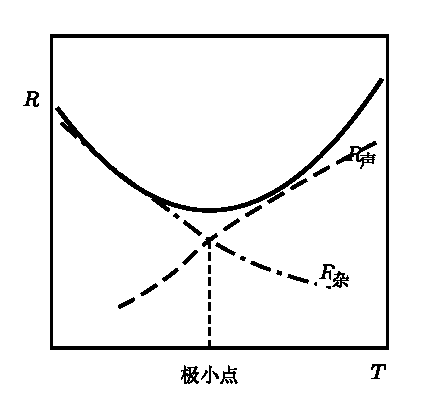
\includegraphics[width=5.5cm]{fig11-8.pdf}\\[0.3em]
{\small （$R=R_{\text{声子}}+R_{\text{杂质}}$）}\\[0.2em]
{\small 图 11.8\quad 电阻极小示意图}
\end{minipage}
\end{center}

\subsection*{1. 近藤的工作}

由于电阻极小现象可以在杂质浓度非常低的情况下被观察到（杂质原子浓度小于 $10^{-4}\%$），因此电阻极小是孤立磁杂质与传导电子间相互作用特征的反映，而不是磁杂质之间相互作用所造成的.近藤采用单个磁性杂质与传导电子之间的s-d交换模型描述稀磁合金的问题，他假定磁性杂质位于原点，具有确定的自旋S，则根据式(11.3.1)、(11.3.22)和(11.3.25)系统的总哈密顿量为
\begin{equation}
  \mathscr{H}=\sum_{k,\,\mu}\varepsilon_{k}C^{+}_{k\mu}C_{k\mu}
  -\biggl(\frac{J}{N}\biggr)\sum_{k,\,k'}\sum_{\mu,\,\mu'}
  \hat{\boldsymbol{S}}\cdot\hat{\boldsymbol{\sigma}}_{\mu\mu'}\,
  C^{+}_{k\mu}C_{k'\mu'}
\end{equation}
式(11.5.2)又称近藤哈密顿量.其中s-d交换作用部分
\begin{equation}
  \mathscr{H}_{\mathrm{s}\text{-}\mathrm{d}}
  =-\biggl(\frac{J}{N}\biggr)\sum_{k,\,k'}\sum_{\mu,\,\mu'}
  \Bigl\{\hat{S}^{z}\hat{\sigma}^{z}_{\mu\mu'}
  +\frac{1}{2}\hat{S}^{+}\hat{\sigma}^{-}_{\mu\mu'}
  +\frac{1}{2}\hat{S}^{-}\hat{\sigma}^{+}_{\mu\mu'}\Bigr\}
  C^{+}_{k\mu}C_{k'\mu'}
\end{equation}
由于 $\hat{S}^{\pm}$ 代表杂质自旋上升及下降算符，$\hat{\sigma}^{\pm}$ 描述传导电子的自旋上升及下降.因此，式(11.5.3)中第一项为非自旋倒逆（non spin-flip）互作用，第二、三项是自旋倒逆（spin-flip）部分，它们涉及电子自旋上升（或下降）与杂质自旋下降（或上升）同时发生的散射过程，因为耦合常数的绝对值 $|J|$ 一般比传导电子的费密能 $E_{\mathrm{F}}$ 小得多，所以近藤最初的计算是用微扰论作出的.他讨论了电子从初态 $(\boldsymbol{k},\mu)$ 散射到终态 $(\boldsymbol{k}',\mu')$，同时杂质自旋从 $\alpha$ 态变为 $\alpha'$ 态的散射概率.在一级近似下，跃迁矩阵元为
\begin{equation}
  T^{(1)}_{\mu'\alpha',\,\mu\alpha}
  =-\biggl(\frac{J}{N}\biggr)\hat{\boldsymbol{\sigma}}_{\mu'\mu}
  \cdot\hat{\boldsymbol{S}}_{\alpha'\alpha}
\end{equation}
$T^{(1)}$ 又称一级散射振幅.这里涉及电子自旋从 $\mu$ 变为 $\mu'$ 的下列4种过程：
\begin{equation}
\left.
\begin{aligned}
  &(\boldsymbol{k}\uparrow)\to(\boldsymbol{k}'\uparrow);
  \ (\boldsymbol{k}\downarrow)\to(\boldsymbol{k}'\downarrow)\\
  &(\boldsymbol{k}\uparrow)\to(\boldsymbol{k}'\downarrow);
  \ (\boldsymbol{k}\downarrow)\to(\boldsymbol{k}'\uparrow)
\end{aligned}\right\}
\end{equation}
相应的 $T^{(1)}$ 分别为
\begin{equation}
  \mp\biggl(\frac{J}{N}\biggr)\hat{S}^{z},
  \qquad \biggl(\frac{J}{N}\biggr)\hat{S}^{\pm}
\end{equation}
因此，由 $T^{(1)}$ 模的平方求出的玻恩近似散射概率正比于
\begin{equation}
  J^{2}\biggl\{(\hat{S}^{z})^{2}
  +\frac{1}{2}\bigl(\hat{S}^{+}\hat{S}^{-}
  +\hat{S}^{-}\hat{S}^{+}\bigr)\biggr\}
  =J^{2}S(S+1)
\end{equation}
是和温度无关的项，只能给出剩余电阻
\begin{equation}
  R_{0}=AJ^{2}S(S+1)
\end{equation}
式(11.5.8)与 $R_{\text{声子}}$ 组合不能说明电阻极小.显然，更重要的过程应当出现在散射振幅（即散射矩阵）的高阶近似中，对于二级微扰过程，散射要通过中间状态 $(\boldsymbol{k}'',\mu'')$ 进行.这里应当区分两种情况，(i)在 $(\boldsymbol{k}'',\mu'')$ 中间态上未被电子占据；(ii)已被电子占据.若以从 $(\boldsymbol{k}\downarrow)$ 态到 $(\boldsymbol{k}'\downarrow)$ 态经历自旋倒逆中间散射过程为例，则对于情况(i)由图11.9(a)描述，称为电子中间态过程.因为，$(\boldsymbol{k}\downarrow)$ 电子先跃迁到 $(\boldsymbol{k}''\uparrow)$ 态，然后再跃迁到 $(\boldsymbol{k}'\downarrow)$ 状态，而杂质自旋则经历先下降后上升的变化 $\hat{S}^{+}\hat{S}^{-}$，考虑到中间态电子处于热平衡，因此在 $(\boldsymbol{k}''\uparrow)$ 状态上未被占据概率应等于 $(1-f_{k''})$，$f_{k''}$ 为费密分布函数.于是求得电子中间态过程的二级散射振幅为
\begin{equation}
  \biggl(\frac{J}{N}\biggr)^{2}\sum_{k''}
  \frac{\hat{S}^{+}\hat{S}^{-}}{\varepsilon_{k}-\varepsilon_{k''}}
  (1-f_{k''})
\end{equation}
对于情况(ii)由图11.9(b)描述，属于空穴中间态过程.因为，要先从 $(\boldsymbol{k}''\uparrow)$ 状态上将电子激发到终态 $(\boldsymbol{k}'\downarrow)$，在 $(\boldsymbol{k}''\uparrow)$ 态则留下空穴，然后初态 $(\boldsymbol{k}\downarrow)$ 电子再与中间态 $(\boldsymbol{k}''\uparrow)$ 的空穴复合，因此电子自旋为先下降后上升，相应的杂质自旋则应经历先上升后下降的变化 $\hat{S}^{-}\hat{S}^{+}$，而且由于 $(\boldsymbol{k}''\uparrow)$ 态在热平衡时被占据概率是 $f_{k''}$，所以空穴中间态过程的二级散射振幅为
\begin{equation}
  \biggl(\frac{J}{N}\biggr)^{2}\sum_{k''}
  \frac{\hat{S}^{-}\hat{S}^{+}}{\varepsilon_{k}-\varepsilon_{k''}}f_{k''}
\end{equation}

\begin{center}
\begin{minipage}{9cm}
\centering
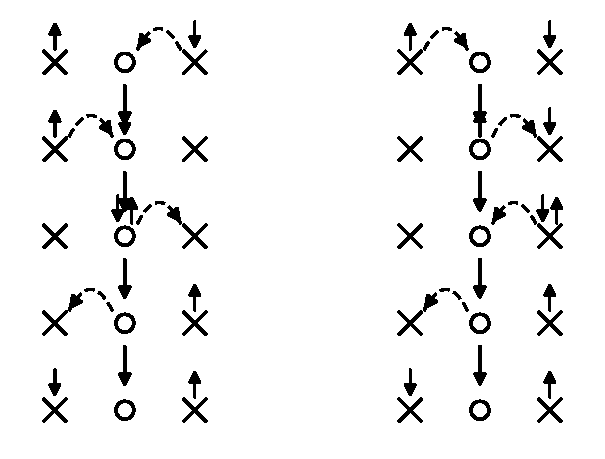
\includegraphics[width=9cm]{fig11-9.pdf}\\[0.3em]
{\small (a) 电子中间态\qquad\qquad (b) 空穴中间态}\\[0.2em]
{\small 图 11.9\quad 自旋倒逆散射的二级过程}
\end{minipage}
\end{center}

以上是s-d互作用中自旋倒逆部分
$\dfrac{1}{2}(\hat{S}^{+}\hat{\sigma}^{-}+\hat{S}^{-}\hat{\sigma}^{+})$
的贡献.对于非自旋倒逆互作用 $\hat{S}^{z}\hat{\sigma}^{z}$ 部分，只需将式(11.5.9)和式(11.5.10)中 $\hat{S}^{+}$ 和 $\hat{S}^{-}$ 用 $\hat{S}^{z}$ 代替，因此求得总的二级散射振幅
\begin{equation}
\begin{aligned}
  T^{(2)}_{\mu'\alpha',\,\mu\alpha}(\varepsilon)
  &=\biggl(\frac{J}{N}\biggr)^{2}\sum_{k''}
  \biggl\{\frac{(\hat{S}^{z})^{2}+\hat{S}^{+}\hat{S}^{-}}
  {\varepsilon-\varepsilon_{k''}}(1-f_{k''})
  +\frac{(\hat{S}^{z})^{2}+\hat{S}^{-}\hat{S}^{+}}
  {\varepsilon-\varepsilon_{k''}}f_{k''}\biggr\}\\
  &=\biggl(\frac{J}{N}\biggr)^{2}\sum_{k''}
  \biggl\{\frac{(\hat{S}^{z})^{2}+\hat{S}^{+}\hat{S}^{-}}
  {\varepsilon-\varepsilon_{k''}}
  -[\hat{S}^{+},\hat{S}^{-}]\frac{f_{k''}}{\varepsilon-\varepsilon_{k''}}\biggr\}
\end{aligned}
\end{equation}
式(11.5.11)后一等式右边第一项主要为非自旋倒逆过程的二级贡献，它仍是与温度无关的.第二项代表自旋倒逆过程的贡献，由于杂质的量子自旋算符具有如下特征：
\begin{equation}
  [\hat{S}^{+},\hat{S}^{-}]
  =\hat{S}^{+}\hat{S}^{-}-\hat{S}^{-}\hat{S}^{+}
  =2\hat{S}^{z}\neq0
\end{equation}
就得到含有温度因子
\begin{equation*}
  f_{k''}=\biggl[\exp\biggl(\frac{\varepsilon_{k''}}{k_{\mathrm{B}}T}\biggr)+1\biggr]^{-1}
\end{equation*}
的散射振幅项.

由于电阻极小是稀磁合金中的普遍现象，具体能带结构对它影响不大，可以采用简化态密度
\begin{equation}
  \rho(\varepsilon)=
  \begin{cases}
    N\rho_{\mathrm{F}} & (\text{当}\ |\varepsilon|<D\ \text{时})\\
    0 & (\text{当}\ |\varepsilon|>D\ \text{时})
  \end{cases}
\end{equation}
其中 $\rho_{\mathrm{F}}$ 代表平均每个电子在费密面上态密度，D代表导带的半宽度.对于能带半填满的金属，D近似等于费密能 $E_{\mathrm{F}}$.

不难计算出下列求和近似为
\begin{equation}
\begin{aligned}
  \biggl(\frac{J}{N}\biggr)\sum_{k''}\frac{f_{k''}}{\varepsilon-\varepsilon_{k''}}
  &\approx J\rho_{\mathrm{F}}\ln
  \frac{\sqrt{\varepsilon^{2}+(k_{\mathrm{B}}T)^{2}}}{E_{\mathrm{F}}}\\
  &=\begin{cases}
    J\rho_{\mathrm{F}}\ln\biggl(\dfrac{k_{\mathrm{B}}T}{D}\biggr)
    & (\text{当}\ \varepsilon=0\ \text{时})\\[0.8em]
    J\rho_{\mathrm{F}}\ln\biggl(\dfrac{|\varepsilon|}{D}\biggr)
    & (\text{当}\ T=0\ \text{K 时})
  \end{cases}
\end{aligned}
\end{equation}
式(11.5.14)表现出对数型的能量及温度函数特征.这正是所希望的，因为总的杂质电阻应该正比于费密面上 $(\varepsilon=0$ 处$)$ 电子被杂质散射的概率，即正比于总散射振幅的模方 $|T^{(1)}+T^{(2)}|^{2}$，其中交叉项提供正比于
\begin{equation}
  J^{3}\rho_{\mathrm{F}}\ln\biggl(\frac{k_{\mathrm{B}}T}{D}\biggr)
\end{equation}
的因子，所以一般说在耦合常数J的3次方项会出现 $\ln T$ 型式的温度因子.近藤\textsuperscript{[18]}算得的磁性杂质电阻为
\begin{equation}
  R_{\text{杂质}}=R_{0}\biggl\{1+4J\rho_{\mathrm{F}}
  \ln\biggl(\frac{k_{\mathrm{B}}T}{D}\biggr)+\cdots\biggr\}
\end{equation}
式(11.5.16)对于 $J>0$ 情况（称铁磁型s-d耦合），只给出随温度降低而减小的杂质电阻，它与热声子电阻 $R_{\text{声子}}$ 的温度变化趋势一致，因此 $J>0$ 情况不导致电阻极小.但是，对于 $J<0$ 情况（称反铁磁型s-d耦合），式(11.5.16)给出 $R_{\text{杂质}}=a-b\ln T$ 项，是随温度降低对数式增长的杂质电阻，它与热声子电阻 $AT^{5}$ 组合正好能说明电阻极小，多数稀磁合金属于 $J<0$ 的材料，因此电阻极小现象普遍能观察到，这些都是近藤计算的成功之处.

\subsection*{2. 近藤效应}

近藤的工作促进了实验工作者对稀磁合金低温特性的进一步研究，发现除电阻极小现象（又称电阻反常）外，还有磁化率、比热容等一系列低温反常现象，通称近藤效应.实验研究的进展主要是如下3方面：

\subsection*{(i) 磁化率反常}

磁化率反常是指杂质磁化率在温度降低时与居里（Curie）定律有偏离，其表示式仍可归结为居里定律的形式
\begin{equation}
  \chi_{\text{杂质}}=\mu^{2}_{\mathrm{eff}}(T)/3k_{\mathrm{B}}T
\end{equation}
{\emergencystretch=2.5em
但是，$\mu_{\mathrm{eff}}$ 是温度的函数，称为杂质的有效磁矩，它仅在高温时与自由原子的确定磁矩
$\mu_{\mathrm{at}}\allowbreak=\mu_{\mathrm{B}}\sqrt{S(S+1)}$
相等，对应于确定的自旋S.实验表明，随着温度降低 $\mu_{\mathrm{eff}}(T)$ 将连续减小，并在 $T\to0$ K时，$\mu_{\mathrm{eff}}\to0$，最后有效磁矩消失.图11.10是对AuV合金磁化率测量所得出 $\mu_{\mathrm{eff}}$ 曲线.由于磁化率是测定磁化强度的z分量，因此实验结果表明在 $T=0$ K时\par}
\begin{equation}
  \langle\hat{S}^{z}\rangle=0
\end{equation}

\begin{center}
\begin{minipage}{6cm}
\centering
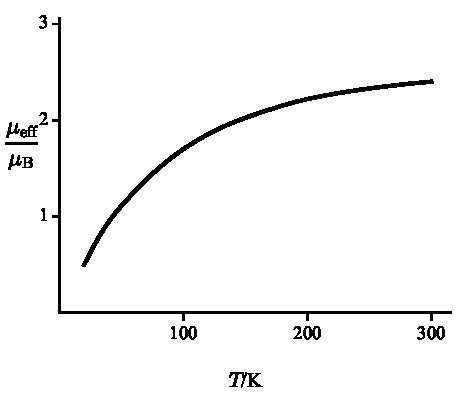
\includegraphics[width=6cm]{fig11-10.pdf}\\{\small 图 11.10\quad 有效杂质磁矩的温度曲线}
\end{minipage}
\end{center}

磁化率反常特征实际上是杂质有效磁矩随温度降低逐渐减小（最后消失）过程在宏观测量上的反映，这是杂质从高温具有确定磁矩 $\mu_{\mathrm{at}}$ 状态向零温度时无磁矩状态的连续变化.由于在s-d模型中是假定杂质具有确定的自旋S，所以 $T=0$ K时所形成的非磁性杂质应当解释为：反铁磁型s-d耦合作用使磁杂质被自旋取向相反的传导电子所包围，从而对杂质磁矩起屏蔽抵消作用，这种抵消倾向随温度降低、热涨落减小而增大，最后在 $T=0$ K时形成一个由杂质和聚集在其周围的反向自旋的传导电子的组合状态，这就是s-d模型中的非磁性杂质态，对应于 $\mu_{\mathrm{eff}}(0)=0$.低温比热容的测量更进一步证实了这种观点.

\subsection*{(ii) 比热容反常}

众所周知，纯金属的低温比热容主要由电子比热容的线性温度律 $\gamma_{\mathrm{e}}T$ 描述.含有一般杂质的金属比热容并不表现出对于线性温度规律的明显偏离，因为这些杂质可以当作是无内结构的外来原子.但是，当金属中含有微量磁性杂质时，比热容将与线性温度规律有严重的偏离，表现为附加在 $\gamma_{\mathrm{e}}T$ 上的一个宽峰曲线，其峰值在低温区，低于电阻极小点.图11.11是CuCr合金的测量曲线.根据热力学，在杂质比热容曲线 $(c_{\text{杂质}}-\ln T)$ 下的面积等于磁杂质在高温和低温时的熵值差
\begin{equation}
\begin{aligned}
  \Delta\mathscr{S}
  &=\int_{0}^{\infty}\frac{c_{\text{杂质}}(T)}{T}\,\mathrm{d}T
  =\mathscr{S}(\infty)-\mathscr{S}(0)\\
  &=k_{\mathrm{B}}\ln(2S+1)
\end{aligned}
\end{equation}
式(11.5.19)中最后一个等式是从实验结果算得的熵差值，其中自旋 $S=3/2$ 正好是Cr在铜中高温测量的自旋值.所以，实验曲线下的面积仅仅等于磁杂质的高温熵值 $k_{\mathrm{B}}\ln(2S+1)$，它要求 $T\to0$ K时磁杂质的熵趋于零，这只能是 $T=0$ K时杂质自旋消失，因为只有这样才能得到零温磁杂质熵
\begin{equation}
  \mathscr{S}(0)=k_{\mathrm{B}}\ln 1=0
\end{equation}
的结果.用s-d模型则解释为零温时（杂质$+$传导电子）系统的总自旋为零.这一总自旋等于零的单重态和磁化率实验所证实的零温度时杂质的非磁特性是一回事，是单个磁杂质与传导电子互作用系统的基态，通常称为近藤单态（Kondo singlet），因为它是非简并的.

\begin{center}
\begin{minipage}{6cm}
\centering
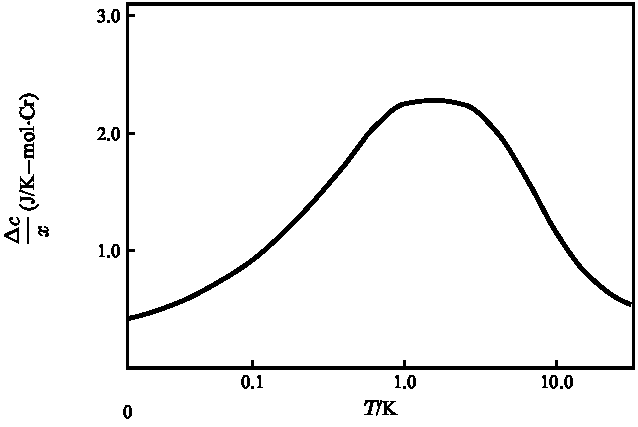
\includegraphics[width=6cm]{fig11-11.pdf}\\{\small 图 11.11\quad CuCr 合金杂质比热容的 ln T 曲线（x 为 Cr 的浓度）}
\end{minipage}
\end{center}

\subsection*{(iii) 低温区的简单平方律}

既然 $T=0$ K时系统的基态是非磁性的近藤单态，与高温时的磁性杂质态完全不同，那么 $T\to0$ K时系统在低温区的特性也应有自己的特征.通过对 $R_{\text{杂质}}$、$\chi_{\text{杂质}}$、$c_{\text{杂质}}$ 的精确实验测量发现，当 $T\to0$ K时它们都与温度T有简单平方的关系：
\begin{equation}
\begin{aligned}
  &R_{\text{杂质}}(T)=R_{\text{杂质}}(0)[1-AT^{2}]\\
  &\chi_{\text{杂质}}(T)=\chi_{\text{杂质}}(0)[1-BT^{2}]\\
  &\frac{(\chi_{\text{杂质}}/\chi_{\mathrm{pauli}})}
  {(c_{\text{杂质}}/c^{\mathrm{e}}_{v})}=2
\end{aligned}
\end{equation}
如图11.12和图11.13所示.由图可知，在 $T\to0$ K时杂质电阻和磁化率的温度曲线都变得平滑化了，这都是由于杂质有效磁矩趋于消失所造成的.例如就杂质电阻而言，在 $T\to0$ K时 $R_{\text{杂质}}$ 趋于饱和，这是因为杂质和周围电子实际上已组成非磁性的近藤单态，从而可以看作是一个"非磁性的外来原子"，它只能提供出与温度几乎无关的剩余电阻，效果与非磁性杂质并无太大差异.

\begin{center}
\begin{minipage}{5cm}
\centering
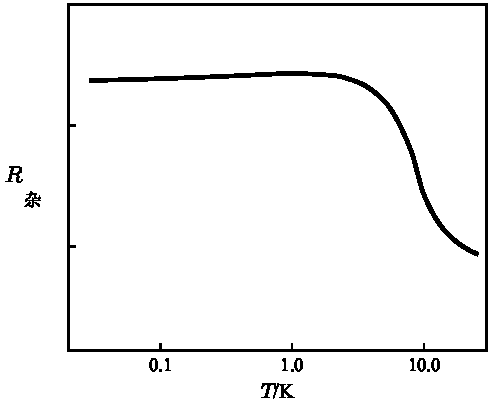
\includegraphics[width=5cm]{fig11-12.pdf}\qquad
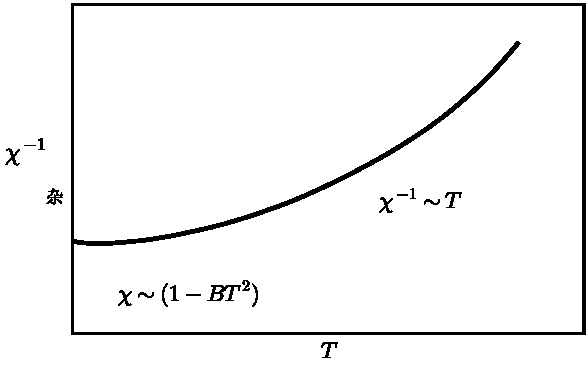
\includegraphics[width=5cm]{fig11-13.pdf}\\[0.3em]
{\small 图 11.12\quad 低温杂质电阻的温度曲线(CuFe 合金)
\qquad 图 11.13\quad 杂质磁化率的温度曲线}
\end{minipage}
\end{center}

综上所述，实验告诉我们近藤效应的本质是金属中单个杂质从磁性状态向非磁性状态的一种连续过渡，在 $T=0$ K时系统的基态是总自旋等于零的单重态.电阻极小，磁化率和比热容的反常等现象都是这一变化在宏观测量上的反映.但是"1"中的微扰计算不适用于低温区，不能用来描述近藤单态.

\subsection*{3. 近藤单态的初步理论}

这里仅介绍芳田奎\textsuperscript{[19]}关于单个磁杂质与传导电子互作用系统的基态理论.他研究 $T=0$ K时一个 $S=1/2$ 的局域自旋与填满的费密球外一个附加电子的s-d耦合系统.把费密球内电子当作自由电子处理，忽略它们可能被杂质散射到球外的复杂情况.因此，费密球的存在仅仅起禁止附加电子占据 $\varepsilon_{k}<0$ 状态的衬底作用.这样做可将近藤哈密顿量（多体哈密顿量）简化为二体问题，与超导理论中的库柏对模型相类似.芳田奎的简化哈密顿量取为
\begin{equation}
  \mathscr{H}_{\mathrm{red}}=\sum_{k,\,\mu}\varepsilon_{k}C^{+}_{k\mu}C_{k\mu}
  -\biggl(\frac{J}{N}\biggr)\sum_{k,\,k'>k_{\mathrm{F}}}\sum_{\mu,\,\mu'}
  \hat{\boldsymbol{S}}\cdot\hat{\boldsymbol{\sigma}}_{\mu\mu'}\,
  C^{+}_{k\mu}C_{k'\mu'}
\end{equation}
与式(11.5.2)相比较可知芳田奎的哈密顿量只考虑了费密球外附加电子与杂质的s-d交换作用.我们可设 $S=1/2$ 局域自旋与传导电子系统的状态为
\begin{equation}
  |\psi\rangle=\sum_{k>k_{\mathrm{F}}}\Gamma_{k}
  \bigl(C^{+}_{k\downarrow}|\uparrow\rangle
  \mp C^{+}_{k\uparrow}|\downarrow\rangle\bigr)|F\rangle
\end{equation}
$|\psi\rangle$ 满足薛定谔方程
\begin{equation}
  (\mathscr{H}_{\mathrm{red}}-E)|\psi\rangle=0
\end{equation}
其中 $|\uparrow\rangle$、$|\downarrow\rangle$ 代表局域自旋朝上及朝下状态，"$-$"代表杂质与附加电子组成的单重态，"$+$"为三重态，包括了芳田奎模型中所有可能组态.$|F\rangle$ 是自由电子的费密球基态，在 $T=0$ K时有
\begin{equation}
\begin{aligned}
  &C^{+}_{k\mu}|F\rangle=0\quad(\text{当}\ \varepsilon_{k}<0\ \text{时})\\
  &C_{k\mu}|F\rangle=0\quad(\text{当}\ \varepsilon_{k}>0\ \text{时})
\end{aligned}
\end{equation}
费密球态的哈密顿量为
\begin{equation}
  \mathscr{H}^{\mathrm{F}}_{0}
  =\sum_{k<k_{\mathrm{F}}}\sum_{\mu}\varepsilon_{k}C^{+}_{k\mu}C_{k\mu}
\end{equation}
相应的能量设为 $E_{\mathrm{g}}$，它满足方程
$(\mathscr{H}^{\mathrm{F}}_{0}-E_{\mathrm{g}})|F\rangle=0$.
显然，$|\psi\rangle$ 也满足方程
\begin{equation}
  (\mathscr{H}^{\mathrm{F}}_{0}-E_{\mathrm{g}})|\psi\rangle=0
\end{equation}
式(11.5.24)与式(11.5.27)相减得
\begin{equation}
  (\overline{\mathscr{H}}-\overline{E})|\psi\rangle=0
\end{equation}
这里
\begin{equation}
  \overline{\mathscr{H}}
  =\sum_{k>k_{\mathrm{F}}}\sum_{\mu}\varepsilon_{k}C^{+}_{k\mu}C_{k\mu}
  -\frac{J}{N}\sum_{k,\,k'>k_{\mathrm{F}}}\sum_{\mu,\,\mu'}
  \hat{\boldsymbol{S}}\cdot\hat{\boldsymbol{\sigma}}_{\mu\mu'}\,
  C^{+}_{k\mu}C_{k'\mu'}
\end{equation}
只涉及费密球外问题，而
\begin{equation}
  \overline{E}=E-E_{\mathrm{g}}
\end{equation}
代表局域自旋与费密球外附加电子的束缚能.用共轭态向量
\begin{equation*}
  \langle F|\bigl(C_{k\downarrow}\langle\uparrow|
  \mp C_{k\uparrow}\langle\downarrow|\bigr)
\end{equation*}
左乘式(11.5.28)，并利用对易式
\begin{equation}
\begin{aligned}
  &[C^{+}_{k\mu},C_{k'\mu'}]_{+}=\delta_{kk'}\delta_{\mu\mu'}\\
  &[C^{+}_{k\mu},C^{+}_{k'\mu'}]_{+}
  =[C_{k\mu},C_{k'\mu'}]_{+}=0
\end{aligned}
\end{equation}
和局域自旋关系
\begin{equation}
\begin{aligned}
  &\hat{S}^{\pm}|\uparrow\rangle
  =\begin{cases}0&(+)\smallskip\\|\downarrow\rangle&(-)\end{cases}\\
  &\hat{S}^{\pm}|\downarrow\rangle
  =\begin{cases}|\uparrow\rangle&(+)\smallskip\\0&(-)\end{cases}\\
  &\hat{S}^{z}|\alpha\rangle=\pm\frac{1}{2}|\alpha\rangle
  \qquad\alpha=\begin{cases}\uparrow\\\downarrow\end{cases}
\end{aligned}
\end{equation}
容易算得对于单重态 $\Gamma_{k}$ 满足方程
\begin{equation}
  2(\varepsilon_{k}-\overline{E})\Gamma_{k}
  +\frac{3J}{N}\sum_{k'>k_{\mathrm{F}}}\Gamma_{k'}=0
\end{equation}
对于三重态，$\Gamma_{k}$ 的方程为
\begin{equation}
  2(\varepsilon_{k}-\overline{E})\Gamma_{k}
  -\frac{J}{N}\sum_{k'>k_{\mathrm{F}}}\Gamma_{k'}=0
\end{equation}
与库柏对问题相似，用 $2(\varepsilon_{k}-\overline{E})$ 除式(11.5.33)和式(11.5.34)，并对k求和.考虑到 $\Gamma_{k}$ 有非零解存在，因此可利用关系
\begin{equation}
  \sum_{k>k_{\mathrm{F}}}\Gamma_{k}=\text{常数}
\end{equation}
消去 $\Gamma_{k}$.对于单重态得到
\begin{equation}
  1+\frac{3J}{2N}\sum_{k>k_{\mathrm{F}}}
  \frac{1}{\varepsilon_{k}-\overline{E}}=0
\end{equation}
而三重态则为
\begin{equation}
  1-\frac{J}{2N}\sum_{k>k_{\mathrm{F}}}
  \frac{1}{\varepsilon_{k}-\overline{E}}=0
\end{equation}
采用简化态密度式(11.5.13)计算求和
\begin{equation}
\begin{aligned}
  \frac{J}{N}\sum_{k>k_{\mathrm{F}}}\frac{1}{\varepsilon_{k}-\overline{E}}
  &\approx J\rho_{\mathrm{F}}\int_{0}^{D}
  \frac{\mathrm{d}\varepsilon}{\varepsilon-\overline{E}}\\
  &=J\rho_{\mathrm{F}}\ln\biggl[\frac{\overline{E}-D}{\overline{E}}\biggr]
\end{aligned}
\end{equation}
当 $|J|\rho_{\mathrm{F}}\ll1$ 时，求得对于反铁磁型s-d耦合 $(J<0)$ 单重态的束缚能为
\begin{equation}
  \overline{E}_{\mathrm{s}}\approx
  -D\exp\biggl[-\frac{2}{3|J|\rho_{\mathrm{F}}}\biggr]
  \qquad(J<0)
\end{equation}
而三重态 $E_{\mathrm{t}}\approx D$ 是不稳定的.只有当 $J>0$ 时三重态才是稳定的
\begin{equation}
  \overline{E}_{\mathrm{t}}\approx
  -D\exp\biggl[-\frac{2}{|J|\rho_{\mathrm{F}}}\biggr]
  \qquad(J>0)
\end{equation}
这时单重态不稳定.

由于近藤效应只是 $J<0$ 时稀磁合金的特征，因此芳田奎的理论告诉我们系统的基态是近藤单态，与实验结果一致.

芳田奎的基态理论忽略了与费密球内电子的相互作用，显然过于粗糙.事实上在低温区近藤问题是很复杂的，由于杂质原子本身具有内自由度（自旋的 $2S+1$ 个取向），当第一个电子通过s-d互作用被散射后，杂质自旋取向要发生变化，这种自旋状态的改变又将直接影响第二个电子在此杂质上的散射，因此相继在杂质上被散射的电子之间存在着通过杂质的间接相互作用，这是一种关联效应.随着温度降低，热涨落减小，关联效应将越来越强，以至在很低温度时任何一个电子的散射都将和系统中所有其它 $(N-1)$ 个电子的运动状态牵连在一起，这里涉及到必须同时考虑所有粒子相互作用的真正多体问题.这一困难直到20世纪70年代在统计力学发展的基础上才得到真正解决，1975年，威尔逊（K.G.Wilson）\textsuperscript{[20]}用实空间重正化群方法严格证明了 $T=0$ K时系统的基态是近藤单态，推广于 $T\neq0$ K情况所计算的磁化率曲线在全温区也与实验一致.威尔逊解只是数值解，1980年，美国\textsuperscript{[21]}和（前）苏联学者\textsuperscript{[22]}应用贝脱方案（Bethe ansatz）又求得了单杂质近藤问题的严格解析解，至此问题才算解决.

最后，还应指出在单杂质的近藤问题中存在一个特征温度 $T_{\mathrm{K}}$，称 $T_{\mathrm{K}}$ 为近藤温度，它是大致划分系统从高温 $(T\gg T_{\mathrm{K}})$ 磁矩态向低温 $(T\ll T_{\mathrm{K}})$ 非磁态渡越的特征温度.当 $T\gg T_{\mathrm{K}}$ 时磁杂质满足居里-外斯定律，其杂质电阻由式(11.5.16)描述，表现为独立磁离子特性，而当 $T\ll T_{\mathrm{K}}$ 时，由于多体关联，局域磁矩将被传导电子屏蔽，形成非磁性的近藤单态，而 $k_{\mathrm{B}}T_{\mathrm{K}}$ 则定义为零温时形成单态系统所降低的能量 $(-\overline{E}_{\mathrm{s}})$.芳田奎等人经过努力，成功地计入了含无穷个电子-空穴对激发的主导项，求得的 $\overline{E}_{\mathrm{s}}$ 相当于将式(11.5.39)的指数中(2/3)因子用(1/2)代替，这时
\begin{equation}
  k_{\mathrm{B}}T_{\mathrm{K}}\equiv-\overline{E}_{\mathrm{s}}
  =D\exp\biggl[-\frac{1}{2\rho_{\mathrm{F}}|J|}\biggr]
\end{equation}
其中D为导带的半宽度，而费密面上传导电子的态密度取为
\begin{equation}
  \rho_{\mathrm{F}}=1/2D
\end{equation}
详细的讨论可参阅修森（Hewson）的专著（文献[24]）.

\section{施里弗-沃尔夫变换}

讲的是如何从安德逊模型导出s-d交换模型.在历史上是施里弗和沃尔夫（Wolff）\textsuperscript{[23]}采用类似于式(5.5.8)—式(5.5.11)的正则变换方法消去安德逊模型中s-d混合作用［式(11.2.4)］的一阶项，首先导出了描述近藤效应的s-d交换模型.因此，人们就将上述两个模型之间的转换关系称为施里弗-沃尔夫变换.在本节中我们将采用投影算符技巧\textsuperscript{[24]}作推导，这样做在物理图像上更为清楚.

从轨道非简并的安德逊模型式(11.2.5)出发，在无外磁场和略去s-d混合作用强度对k的依赖（即取 $V_{kd}=V$）条件下，将哈密顿量写为
\begin{equation}
  H=\sum_{k,\,\sigma}E_{k}C^{+}_{k\sigma}C_{k\sigma}
  +\sum_{\sigma}E_{\mathrm{d}}n_{\mathrm{d}\sigma}
  +Un_{\mathrm{d}\uparrow}n_{\mathrm{d}\downarrow}
  +H_{\mathrm{mix}}
\end{equation}
其中
\begin{equation}
  H_{\mathrm{mix}}=V\sum_{k,\,\sigma}
  \bigl(d^{+}_{\sigma}C_{k\sigma}+C^{+}_{k\sigma}d_{\sigma}\bigr)
\end{equation}
\begin{equation}
  n_{\mathrm{d}\sigma}=d^{+}_{\sigma}d_{\sigma}
\end{equation}
注意到安德逊模型在 $V=0$ 时，由于局域的d电子不与传导电子相耦合，杂质的两个d轨道能级分别为 $E_{\mathrm{d}}$ 与 $E_{\mathrm{d}}+U$.这时系统存在3种不同的d电子组态：(i)两个d能级均为零占据，对应的总能量为 $E_{0}=0$；(ii)自旋 $\sigma$ 的单占据组态，总能量为 $E_{1\sigma}=E_{\mathrm{d}}$，其中 $\sigma=\uparrow$ 或 $\downarrow$；(iii)双占据组态，两个能级分别被一个自旋 $\uparrow$ 和一个自旋 $\downarrow$ 的电子所占据，对应的总能量为 $2E_{\mathrm{d}}+U$，如图11.14所示.

\begin{center}
\begin{minipage}{9cm}
\centering
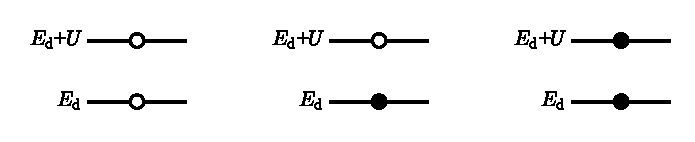
\includegraphics[width=9cm]{fig11-14.pdf}\\[0.3em]
{\small (a) 零占据\qquad\qquad (b) 单占据\qquad\qquad (c) 双占据}\\[0.2em]
{\small 图 11.14\quad 杂质上的 d 电子组态}
\end{minipage}
\end{center}

如果基态对应于单占据组态，则要求 $E_{\mathrm{d}}<E_{\mathrm{F}}$ 和 $E_{\mathrm{d}}+U>E_{\mathrm{F}}$，若再取传导电子的费密能级 $E_{\mathrm{F}}$ 为能量的原点，则只有单占据组态的总能量小于零，而双占据与零占据组态的总能量将大于或等于零.这时杂质的基态将是存在一个自旋 $\uparrow$ 或 $\downarrow$ 的有局域矩的磁性状态，而激发态则对应于零占据或双占据的无局域磁矩状态.我们的问题是要研究当局域d态与传导电子之间存在混合作用（即 $V\neq0$）时安德逊模型中的局域磁矩特征.我们将证明，当V足够弱时安德逊模型可直接简化为§3中的s-d交换模型.

在一般情况下，可以将安德逊模型在希尔伯特空间划分为3个子空间，并相应地引入3套投影算符
\begin{equation}
\begin{aligned}
  &P_{0}=(1-n_{\mathrm{d}\uparrow})(1-n_{\mathrm{d}\downarrow})\\
  &P_{1}=n_{\mathrm{d}\uparrow}(1-n_{\mathrm{d}\downarrow})
  +n_{\mathrm{d}\downarrow}(1-n_{\mathrm{d}\uparrow})\\
  &P_{2}=n_{\mathrm{d}\uparrow}n_{\mathrm{d}\downarrow}
\end{aligned}
\end{equation}
其中 $P_{n}$ 代表投影到占据数 $n=0,\,1,\,2$ 的空占据，单占据和双占据子空间的算符，并且满足投影算符的基本规则：
\begin{equation*}
\begin{aligned}
  &P^{2}_{n}=P_{n}\qquad(n=0,\,1,\,2)\\
  &P_{0}P_{1}=P_{1}P_{2}=P_{0}P_{2}=0
\end{aligned}
\end{equation*}
相应地在全希尔伯特空间中，系统的总波函数 $\varPsi$ 可由3个子空间中的分量 $\psi_{0}$、$\psi_{1}$ 和 $\psi_{2}$ 作线性组合构成，这时薛定谔方程 $H\varPsi=E\varPsi$ 可以表示为
\begin{equation}
  \begin{pmatrix}
    H_{00}&H_{01}&H_{02}\\
    H_{10}&H_{11}&H_{12}\\
    H_{20}&H_{21}&H_{22}
  \end{pmatrix}
  \begin{pmatrix}\psi_{0}\\\psi_{1}\\\psi_{2}\end{pmatrix}
  =E\begin{pmatrix}\psi_{0}\\\psi_{1}\\\psi_{2}\end{pmatrix}
\end{equation}
其中 $H_{nn'}=P_{n}HP_{n'}$.对于安德逊模型，由于不存在同时产生和消灭两个d电子的互作用，所以 $H_{02}=H_{20}=0$，其它的非对角矩阵元如 $H_{01}$ 和 $H_{12}$ 均来自 $H_{\mathrm{mix}}$.运用泡利原理和费密子的算符等式 $n^{2}_{\mathrm{d}\sigma}=n_{\mathrm{d}\sigma}$ 可导出

\begin{subequations}
\begin{equation}
  H_{01}=P_{0}HP_{1}=P_{0}H_{\mathrm{mix}}P_{1}
  =V\sum_{k,\,\sigma}C^{+}_{k\sigma}
  \bigl(1-n_{\mathrm{d}\bar{\sigma}}\bigr)d_{\sigma}
\end{equation}
\begin{equation}
  H_{12}=P_{1}HP_{2}=P_{1}H_{\mathrm{mix}}P_{2}
  =V\sum_{k,\,\sigma}C^{+}_{k\sigma}d_{\sigma}n_{\mathrm{d}\bar{\sigma}}
\end{equation}
\end{subequations}

并且矩阵是厄米的，有 $H_{10}=H^{+}_{01}$ 与 $H_{21}=H^{+}_{12}$ 关系.

现在讨论存在 $H_{\mathrm{mix}}$ 项时的d轨道单占据解.为此，从式(11.6.5)中消去 $\psi_{0}$ 和 $\psi_{2}$ 态，求得在单占据子空间的一个等效方程
\begin{equation}
  \widetilde{H}\psi_{1}=E_{1}\psi_{1}
\end{equation}
其中
\begin{equation}
  \widetilde{H}=H_{11}
  +H_{12}(E-H_{22})^{-1}H_{21}
  +H_{10}(E-H_{00})^{-1}H_{01}
\end{equation}
代表单占据子空间中的有效哈密顿量.到此为止，我们尚未作任何近似，式(11.6.8)仍是严格的.施里弗-沃尔夫变换则只是在准至V二阶的微扰范围内计入系统从单占据向零占据和双占据等状态的虚激发，这时 $(E-H_{22})$ 可近似用 $V=0$ 时单占与双占态的能量差 $(E_{k'}-E_{\mathrm{d}}-U)$ 代替，它表示传导电子 $E_{k'}$ 进入杂质d轨道的高能级 $E_{\mathrm{d}}+U$.类似的，对于 $(E-H_{00})$ 也可用 $(E_{\mathrm{d}}-E_{k})$ 代替，表明单占据的 $E_{\mathrm{d}}$ 电子逸出d轨道成为传导电子 $E_{k}$.再运用式(11.6.6)，在准至V二阶条件下，可将式(11.6.8)中的两个虚激项分别写为

\begin{subequations}
\begin{equation}
\begin{aligned}
  H_{12}(E-H_{22})^{-1}H_{21}
  &=\sum_{k,\,k',\,\sigma,\,\sigma'}
  \frac{V^{2}}{(U+E_{\mathrm{d}}-E_{k'})}(-1)\\
  &\qquad\times C^{+}_{k\sigma}C_{k'\sigma'}d_{\sigma}
  n_{\mathrm{d}\bar{\sigma}}d^{+}_{\sigma'}n_{\mathrm{d}\bar{\sigma}'}
\end{aligned}
\end{equation}
\begin{equation}
\begin{aligned}
  H_{10}(E-H_{00})^{-1}H_{01}
  &=\sum_{k,\,k',\,\sigma,\,\sigma'}
  \frac{V^{2}}{(E_{\mathrm{d}}-E_{k})}(-1)
  C^{+}_{k\sigma}C_{k'\sigma'}d^{+}_{\sigma'}
  \bigl(1-n_{\mathrm{d}\bar{\sigma}'}\bigr)\\
  &\qquad\times d_{\sigma}\bigl(1-n_{\mathrm{d}\bar{\sigma}'}\bigr)
\end{aligned}
\end{equation}
\end{subequations}

在满足单占据条件 $n_{\mathrm{d}}=n_{\mathrm{d}\uparrow}+n_{\mathrm{d}\downarrow}=1$ 时，根据自旋 $\dfrac{1}{2}$ 的算符等式：
\begin{equation}
\left.
\begin{aligned}
  &\hat{S}^{z}=\frac{1}{2}
  (d^{\dagger}_{\uparrow}d_{\uparrow}
  -d^{\dagger}_{\downarrow}d_{\downarrow})\\
  &\hat{S}^{+}=d^{\dagger}_{\uparrow}d_{\downarrow}\\
  &\hat{S}^{-}=d^{\dagger}_{\downarrow}d_{\uparrow}
\end{aligned}\right\}
\end{equation}
经简单运算，可将式(11.6.9a)中算符归并为如下3种类型：
\begin{equation*}
\begin{aligned}
  &\text{(i)}\ \sigma=\downarrow\ \text{与}\ \sigma'=\uparrow\ \text{项：}
  \ C^{+}_{k\downarrow}C_{k'\uparrow}d^{\dagger}_{\uparrow}d_{\downarrow}
  =\hat{S}^{+}C^{+}_{k\downarrow}C_{k'\uparrow}\\
  &\text{(ii)}\ \sigma=\uparrow\ \text{与}\ \sigma'=\downarrow\ \text{项：}
  \ C^{+}_{k\uparrow}C_{k'\downarrow}d^{\dagger}_{\downarrow}d_{\uparrow}
  =\hat{S}^{-}C^{+}_{k\uparrow}C_{k'\downarrow}\\
  &\text{(iii)}\ \sigma=\sigma'=\uparrow\ \text{和}\ \sigma=\sigma'=\downarrow\ \text{项：}
  \ \hat{S}^{z}\bigl(C^{+}_{k\uparrow}C_{k'\uparrow}
  -C^{+}_{k\downarrow}C_{k'\downarrow}\bigr)\\
  &\hphantom{\text{(iii)}\ \sigma=\sigma'=\uparrow\ \text{和}\ \sigma=\sigma'=\downarrow\ \text{项：}\ \hat{S}^{z}(\cdots)\ }
  -\frac{1}{2}\sum_{\sigma}C^{+}_{k\sigma}C_{k'\sigma}
\end{aligned}
\end{equation*}
由此求得
\begin{equation}
\begin{aligned}
  H_{12}(E-H_{22})^{-1}H_{21}
  &=\sum_{k,\,k'}\frac{V^{2}}{(U+E_{\mathrm{d}}-E_{k'})}
  \bigl\{\bigl[\hat{S}^{z}\bigl(C^{+}_{k\uparrow}C_{k'\uparrow}
  -C^{+}_{k\downarrow}C_{k'\downarrow}\bigr)\\
  &\qquad+\hat{S}^{+}C^{+}_{k\downarrow}C_{k'\uparrow}
  +\hat{S}^{-}C^{+}_{k\uparrow}C_{k'\downarrow}\bigr]
  -\frac{1}{2}\sum_{\sigma}C^{+}_{k\sigma}C_{k'\sigma}\bigr\}
\end{aligned}
\end{equation}
类似的讨论可证明
\begin{equation}
\begin{aligned}
  H_{10}(E-H_{00})^{-1}H_{01}
  &=\sum_{k,\,k'}\frac{V^{2}}{(E_{k}-E_{\mathrm{d}})}
  \bigl\{\bigl[\hat{S}^{z}\bigl(C^{+}_{k\uparrow}C_{k'\uparrow}
  -C^{+}_{k\downarrow}C_{k'\downarrow}\bigr)\\
  &\qquad+\hat{S}^{+}C^{+}_{k\downarrow}C_{k'\uparrow}
  +\hat{S}^{-}C^{+}_{k\uparrow}C_{k'\downarrow}\bigr]
  +\frac{1}{2}\sum_{\sigma}C^{+}_{k\sigma}C_{k'\sigma}\bigr\}
\end{aligned}
\end{equation}
再考虑到略去常数项 $E_{\mathrm{d}}$ 后，$H_{11}$ 简化为传导电子的自由项
\begin{equation}
  H_{o}=\sum_{k,\,\sigma}E_{k}C^{+}_{k\sigma}C_{k\sigma}
\end{equation}
将上述结果代入式(11.6.8)，求得在单占据子空间中的有效哈密顿量
\begin{equation}
  \widetilde{H}=H_{o}+H_{\mathrm{p}}+H_{\mathrm{sd}}
\end{equation}
其中 $H_{\mathrm{p}}$ 只是一般的杂质势散射项
\begin{equation}
  H_{\mathrm{p}}=\sum_{k,\,k',\,\sigma}\frac{V^{2}}{2}
  \biggl\{\frac{1}{(E_{k}-E_{\mathrm{d}})}
  -\frac{1}{(U+E_{\mathrm{d}}-E_{k'})}\biggr\}
  C^{+}_{k\sigma}C_{k'\sigma}
\end{equation}
而 $H_{\mathrm{sd}}$ 则代表与杂质的自旋自由度有关的s-d交换作用项
\begin{equation}
  H_{\mathrm{sd}}=-\sum_{k,\,k'}J_{kk'}
  \bigl\{\hat{S}^{z}\bigl(C^{+}_{k\uparrow}C_{k'\uparrow}
  -C^{+}_{k\downarrow}C_{k'\downarrow}\bigr)
  +\hat{S}^{+}C^{+}_{k\downarrow}C_{k'\uparrow}
  +\hat{S}^{-}C^{+}_{k\uparrow}C_{k'\downarrow}\bigr\}
\end{equation}
其耦合强度为
\begin{equation}
  J_{kk'}=-V^{2}\biggl\{\frac{1}{(E_{k}-E_{\mathrm{d}})}
  +\frac{1}{(U+E_{\mathrm{d}}-E_{k'})}\biggr\}
\end{equation}
由于与杂质自旋相互作用的传导电子均位于费密面附近，人们可以将上式中的 $E_{k}$ 与 $E_{k'}$ 近似取为 $E_{\mathrm{F}}$，再考虑到在局域矩区域有 $U+E_{\mathrm{d}}>E_{\mathrm{F}}>E_{\mathrm{d}}$ 条件，因此 $J_{kk'}<0$，说明在杂质自旋与传导电子自旋之间的耦合是反铁磁型s-d耦合，它导致近藤效应.在强关联极限下可取 $U\to\infty$，这时s-d交换作用简化为与k及 $k'$ 均无关的耦合常数
\begin{equation}
  J_{kk'}=J=-\frac{V^{2}}{|E_{\mathrm{d}}-E_{\mathrm{F}}|}<0
\end{equation}
这时若略去杂质的一般性势散射效应，$\widetilde{H}$ 将直接写成
\begin{equation}
\begin{aligned}
  \widetilde{H}&=\sum_{k,\,\sigma}E_{k}C^{+}_{k\sigma}C_{k\sigma}
  -J\sum_{k,\,k'}\bigl\{\hat{S}^{z}\bigl(C^{+}_{k\uparrow}C_{k'\uparrow}
  -C^{+}_{k\downarrow}C_{k'\downarrow}\bigr)\\
  &\qquad+\hat{S}^{+}C^{+}_{k\downarrow}C_{k'\uparrow}
  +\hat{S}^{-}C^{+}_{k\uparrow}C_{k'\downarrow}\bigr\}
\end{aligned}
\end{equation}
与描述近藤效应的哈密顿量式(11.5.2)相同.差别仅在于那里的 $(J/N)$ 对应于上式中的J.

综上所述，从单杂质安德逊模型出发，在传导电子与局域电子之间的混合作用V很弱时，研究系统从单占据基态 d$^{1}$ 向零占据态 d$^{0}$ 和双占据态 d$^{2}$ 等激发态的虚跃迁效应，在准至V的二阶近似下证明了这类激发等效于s-d交换作用.因此，人们常说当V很小时安德逊模型可直接过渡到描述近藤效应的s-d交换模型.从物理上讲，s-d交换模型是在d电子满足单占据条件下导出的，在那里d电子的电荷涨落（即杂质的价涨落）效应已被忽略，但是，在安德逊模型中由于存在混合作用V，局域电子与传导电子之间有相互转移，将导致局域电子的电荷涨落（或杂质的价涨落）效应.因此，这两个模型是有区别的，并且后者涉及更为广泛的物理问题.仅当V足够的弱，d$^{0}$ 与 d$^{2}$ 等组态相对于单占据组态 d$^{1}$ 的占据比例小到可以忽略时，安德逊模型才能够用一个不计电荷涨落的s-d交换模型来代替.换句话说，施里弗-沃尔夫变换正是在混合作用十分微弱的条件下，消去V所产生的电荷涨落，代之以一个局域自旋与传导电子自旋的非直接交换作用，使安德逊模型过渡为s-d交换模型，被称为安德逊模型的近藤极限.在此极限下，杂质的电荷涨落被压制，表现为局域自旋矩特征，它与传导电子间的耦合仅产生自旋的取向变化，导致系统的自旋涨落.

安德逊模型存在两个有意义的极限，它们是近藤极限和变价（又称混合价）极限.近藤极限首先要求杂质处于局域矩状态.当 $V=0$ 时，存在局域矩（或单占据基态）的条件已给出为 $E_{\mathrm{d}}<E_{\mathrm{F}}$ 与 $E_{\mathrm{d}}+U>E_{\mathrm{F}}$，物理上对应于要求费密能级位于两个自旋劈裂能级之间.当计入混合作用V之后，系统形成局域矩的条件可近似由外场 $h=0$ 时的自洽方程式(11.2.33)决定，它们是
\begin{equation}
\left.
\begin{aligned}
  \langle n_{\mathrm{d}\uparrow}\rangle
  &=\frac{1}{\pi}\mathrm{arccot}
  \biggl[\frac{E_{\mathrm{d}}-E_{\mathrm{F}}
  +U\langle n_{\mathrm{d}\downarrow}\rangle}{\Gamma}\biggr]\\
  \langle n_{\mathrm{d}\downarrow}\rangle
  &=\frac{1}{\pi}\mathrm{arccot}
  \biggl[\frac{E_{\mathrm{d}}-E_{\mathrm{F}}
  +U\langle n_{\mathrm{d}\uparrow}\rangle}{\Gamma}\biggr]
\end{aligned}\right\}
\end{equation}
其中 $\Gamma=\pi V^{2}\rho^{(0)}(E_{\mathrm{F}})$ 代表杂质d轨的共振线半宽度.显然，当满足下列条件时
\begin{equation}
\begin{gathered}
  E_{\mathrm{d}}<E_{\mathrm{F}},
  \quad E_{\mathrm{d}}+U>E_{\mathrm{F}}\\
  \text{和}\\
  |E_{\mathrm{d}}+U-E_{\mathrm{F}}|,\ |E_{\mathrm{d}}-E_{\mathrm{F}}|\gg\Gamma
\end{gathered}
\end{equation}
存在 $\langle n_{\mathrm{d}\uparrow}\rangle\to1$，$\langle n_{\mathrm{d}\downarrow}\rangle\to0$ 的局域矩解，这时磁杂质的平均电子数并无显著变化，仍保持整数价.应当指出，式(11.6.21)中包含了形成局域磁矩的最有利条件 $\Gamma\ll U$.正是在此强关联与弱杂化条件下，杂质的电荷涨落被压制，安德逊模型才能演化为描述局域自旋矩与传导电子自旋之间的反铁磁型交换作用的s-d交换模型，并用于解释近藤效应.因此，式(11.6.21)是近藤极限（又称整数价极限）的参数条件.在具体运用安德逊模型讨论金属中的过渡和稀土磁性杂质时，人们往往直接从强关联极限 $(U\to\infty)$ 情形出发，由于在 $E_{\mathrm{d}}+U$ 能级上不可能占据电子，近藤极限条件简化为要求 $(E_{\mathrm{d}}-E_{\mathrm{F}})$ 取大的负值，即 $|E_{\mathrm{d}}-E_{\mathrm{F}}|\gg\Gamma$，并可求出一个与k无关的s-d交换作用 $J=-V^{2}/|E_{\mathrm{d}}-E_{\mathrm{F}}|$.安德逊模型的另一个极限出现在 $E_{\mathrm{d}}$ 能级比较接近 $E_{\mathrm{F}}$ 以至 $|E_{\mathrm{d}}-E_{\mathrm{F}}|$ 与 $\Gamma$ 值相近的情形，这时杂质的电荷涨落变得十分重要，在杂质的局域轨道态与传导电子的费密海之间将出现电荷的实际转移，它们不能再用二级微扰的虚激发过程处理，因此施里弗-沃尔夫变换失效，人们必须从 $U=\infty$ 的安德逊模型出发来讨论这一极限情形.由于电荷涨落，磁性杂质不再具有整数价，而是两种或多种价态的混合，这种具有非整数价特征情形被称之为变价极限.典型的例子是高压下的稀土化合物SmS，电荷涨落使Sm$^{2+}$离子有一定概率变为Sm$^{3+}$，使Sm离子处于介乎2价与3价之间的中间价态 Sm$^{\nu+}$（$\nu=2.75$），这类材料也相应地称之为价变（或中间价）化合物.显然，$U=\infty$ 的安德逊模型是讨论金属中磁杂质近藤效应和变价特性的一个良好理论模型，在此模型中，若取 $E_{\mathrm{d}}$ 远远低于 $E_{\mathrm{F}}$，将得到近藤极限，而取 $E_{\mathrm{d}}$ 十分靠近 $E_{\mathrm{F}}$ 又可达变价极限.

近年来，在含有未填满的f壳层稀土（如Ce、4f）及锕系（如U、5f）元素的多元化合物中发现了新的一类固体材料，其中大多数材料具有金属性，其共同的特点是低激发态具有很高的电子有效质量 $(m^{*}/m_{\mathrm{e}}\gg1)$，被称为重电子金属，理论上属于重费密子系统.在重费密子系统中已发现了3种不同的金属型基态.它们是：重费密子超导体（CeCu$_{2}$Si$_{2}$、UBe$_{13}$、UPt$_{3}$等），重费密子磁体（U$_{2}$Zn$_{17}$、UCd$_{11}$、NpBe$_{13}$等）和重费密子液体（CeAl$_{3}$、CeCu$_{6}$、YbCuAl等）.这些材料的零温电子比热容的线性温度系数 $\gamma$ 可高达 $100\sim1000$ mJ/(mol$\cdot$K$^{2}$)，比普通金属的 $\gamma$ 值 $1\sim10$ mJ/(mol$\cdot$K$^{2}$)平均高100倍，最高可达1000倍.由于 $\gamma\sim m^{*}$，而在普通金属中 $m^{*}$ 与自由电子质量 $m_{\mathrm{e}}$ 同量级，因此近期对重费密子系统有效质量的下界大致规定在 $m^{*}\geqslant10\sim100\,m_{\mathrm{e}}$ 的较宽松区域内\textsuperscript{[25]}.这样做可统一概括早期对重费密子系统的"轻量级" $(m^{*}/m_{\mathrm{e}}>10)$、"中等量级" $(m^{*}/m_{\mathrm{e}}>50)$ 以及"重量级" $(m^{*}/m_{\mathrm{e}}>100)$ 等繁琐分类.20世纪90年代以来在4f族化合物（Ce$_{3}$Bi$_{4}$Pt$_{3}$、CeRhSb、CeNiSn）中发现了具有绝缘性基态的重费密子材料，加上早期的绝缘性化合物SmB$_{6}$和YbB$_{12}$构成重费密子系统中新一类，它们具有不同寻常的小能隙 $(\Delta=1\sim10$ meV，对应于 $10\sim100$ K$)$ 半导体特征，称为重费密子半导体或近藤绝缘体，其能隙是温度的函数，并且对掺杂、加压和外磁场均十分敏感，在Ce$_{3}$Bi$_{4}$Pt$_{3}$中，当温度T上升到接近零温 $\Delta$ 值时，或用La替代Ce作掺杂 (La$_{x}$Ce$_{1-x}$)$_{3}$Bi$_{4}$Pt$_{3}$，均可能使能隙消失，这时近藤绝缘体系统过渡为重费密子金属，并具有高的比热容系数，例如 $x=0.3$ 时 $\gamma$ 可高达150 mJ/(mol$\cdot$K$^{2}$)，应属重费密子系统.

从理论上讲，重费密子系统是每个元胞中均含有稀土和锕系离子的晶格系统.高温磁化率测量表明，无论是重费密子金属或半导体均表现为如同独立磁性离子那样满足居里-外斯规律，说明f电子在强关联 $U\gg\Gamma$ 条件下形成了局域磁矩，与金属中含单个磁杂质的近藤问题有相似之处，差别仅在于重费密子材料是近藤离子呈周期性排列的晶格系统，人们称之为近藤晶格系统.由于安德逊模型是描述单杂质近藤问题的良好出发点，人们普遍相信，若将它作周期性推广，构成安德逊晶格模型也将是描述重费密子系统（或近藤晶格）本质特征的一个基本模型.类似于单杂质近藤问题，重费密子系统与近藤晶格也属于 $U\gg\Gamma$ 的强关联电子体系，在具体进行理论处理时，可采用 $U=\infty$ 的安德逊晶格模型.但应注意，在强关联情况下在本章§2中对同格点库仑关联作平均场近似的方案失效，必须寻找处理强关联系统的良好近似，其中之一就是下节中将介绍的隶玻色技巧的平均场近似.

% ============================================================
%  第十一章 强关联电子体系（后半：§7–§11 + 章末参考文献）
%  底本：高等教育出版社《固体理论》第二版；原书印刷页 433–485
%  （PDF 页 = 印刷页 + 20；§7 约自 PDF 453 起）
%  本文件不含 \chapter（章标题在前半 ch11a.tex），
%  直接以 \section{隶玻色子技巧} 开头，节计数器接续 §6。
%
%  公式编号自检（自动编号，每节内从 1 连续，无缺号）：
%    §7  (11.7.1)–(11.7.30)；其中 (11.7.6)、(11.7.25)、(11.7.29)
%        原书即分 a/b(/c) 二级编号，用 subequations 照录；
%    §8  (11.8.1)–(11.8.45)；其中 (11.8.2)、(11.8.7)、(11.8.8)、
%        (11.8.9)、(11.8.11)、(11.8.12)、(11.8.22)、(11.8.33)
%        原书即分 a/b(/c)，subequations 照录；
%    §9  (11.9.1)–(11.9.32)；其中 (11.9.2) 分 a–f、(11.9.5) 分
%        a–f、(11.9.27)(11.9.28)(11.9.29) 分 a/b，照录；
%    §10 (11.10.1)–(11.10.21)；其中 (11.10.2)(4)(5)(6)(8)(9)
%        (11)(13)(15)(16)(17) 原书分 a/b(/c)，照录；
%    §11 (11.11.1)–(11.11.80)；其中 (11.11.39)(11.11.40) 分 a/b。
%    任务单所列"缺号"经逐页核对（PDF 453–505）全部在号：
%    均为上述 subequations 拆号或 OCR tag 残缺，原书无跳号。
%    OCR 编号陷阱甄别：(1.9.4)→(11.9.4)（p451）、(8.24)→
%    (11.8.24)（p446）、(.2a)→(11.8.2a)、"(11.7.2),"→(11.7.28)
%    （p439，正文"式(11.7.28)"互证）、(.10.10)→(11.10.10)、
%    (10.13a)→(11.10.13a)、"(11"→(11.11.38)（p474）、
%    "(1.11.66)"→(11.11.66)、游离的"(11.11.45)""(11.11.50)"
%    "(11.11.62)"均按原书归还本式（p476–478）。
%
%  已修正的 OCR/原书错误（除全角句点转"."、删 ~ 间隔符、收紧
%  \mathrm{d}、< <A|B> > 统一 \langle\langle…\rangle\rangle、
%  拆开行内公式与中文、上标 [N] 转正文等常规项外）：
%  1. 原书 p435 (11.7.7) 首行"E_0X_{σσ}(l)·+"衍一居中点，
%     删（同页 (11.7.8) 对照无此点）。
%  2. 原书 p435 脚注①（赫伯德算符的另一写法，OCR 整条漏失），
%     已按 p455 页脚补录为 \footnote。
%  3. 原书 p436 正文"科尔曼首先注意到约束Ô与隶玻色子表示 Q̂_l
%     中的H是可对易的"语序错乱，按 p456 复原为"约束 Q̂_l 与隶
%     玻色子表示中的 H 是可对易的"。
%  4. (11.7.19) 为跨页一式（p436–437，号在次页末行），OCR 拆成
%     两块，已按原书合并为一号。
%  5. (11.7.20) 末项 OCR 漏 λ，按 p438 补"Nλ(r²-1)"；(11.7.22)
%     原书"{("括号不配对，按文意配平为 {…}。
%  6. (11.8.1) 右端 OCR 乱码"=(1 0;0 1)(η;η)(η;η)."，按 p460
%     复原为单位矩阵。
%  7. (11.8.16) 前正文"带边在±(ω)=±D处"→"ε(ω)=±D"（p443）。
%  8. (11.8.24)(11.8.25) OCR tag 残缺（"8.24"）或编号嵌于式内，
%     按 p446 归还；(11.8.26)(11.8.27) 积分下标 ω_s→ω_a。
%  9. (11.8.33a/b) OCR 残留的 Δ 符号均系噪声，按 p447 复原为
%     Γ̃/Γ、(E_0-μ) 等；(11.8.36) 的 \tilde{ν}→Ṽ（全节统一）。
% 10. (11.8.37) 原书右端印"2π²h²"（h 无杠），照录；分母 E_f 照
%     原书（下标字形近 F，此处按费密能量取 E_F 义，排作 E_F）。
% 11. (11.9.1) 库仑项"n_i n_i ν_i"按 p450 复原为 n_{i↑}n_{i↓}；
%     正文"只能容约N个"→"容纳"（p450）。
% 12. (11.9.2a–f)(11.9.5a–f) 为原书自带二级编号（正文引
%     (11.9.2e)—(11.9.2f)、(11.9.5d)—(11.9.5f) 互证），OCR
%     被拆散的下标按 p451–452 复原。
% 13. 原书 p454 (11.9.17) 第三行首算符印"Ŝ_j^z"而右端为 C_{iσ}
%     算符，按 p454 上下文及 (11.6.10) 改 Ŝ_i^z（原书排印误）。
% 14. 原书 p455 正文"T_h=0 √(dE/dt) 格成立"乱码按 p455 复原为
%     "T_h=0 严格成立"；(11.9.24) 原书第三项印 p_{i+½ŷσ}，
%     按 (11.9.23) 的四项结构改 p_{i+½x̂σ}（原书排印误）。
% 15. (11.9.31) OCR 丢自旋标，按 p460 复原为
%     b_i⁺=(a†_{i↑}d†_{i↓}-a†_{i↓}d†_{i↑})/√2。
% 16. §10 章首"将式(11.9.32)中的 t_eff 与J_eff⟨…⟩乱码"按 p462
%     复原为"与 J_eff 仍用 t 与 J 表示"；φ=arctan(k̂_y/k̂_y)→
%     arctan(k̂_y/k̂_x)（p468）。
% 17. 原书 p466 "从式(9.10.15a)将得到"系原书章号误排，按上下文
%     改为式(11.10.15a)（已在文件头注明）。
% 18. (11.10.19) 原书第四算符印 Ĉ_{i↑}、右端末因子印 f_{j↑}，均
%     演上标 †（且下标 j 误作 i），按单重态配对结构（与 RHS
%     b_i b_j f†_{i↑}f†_{j↓} 对应）复原为 Ĉ†_{j↑}、f†_{j↑}
%     （p466 300dpi 页面核对）。
% 19. 原书 p469 "(11.11.25)"左端与分子均印 χ_0，分子应为泡利磁
%     化率，按 (11.11.19) 改 χ_P；"(11.11.27)"左端原书印 χ_P，
%     按 (11.11.25)(11.11.30) 改 χ_0（均系原书排印误）。
% 20. (11.11.2) 第二项按 p469 复原为 ⟨n_{l↓}⟩n_{l↑}；(11.11.3)
%     (11.11.4)(11.11.7) 的 ⟨n_{lσ̄}⟩ 类下标按 p469 复原。
% 21. (11.11.31) 分母指数按 p473 复原为 e^{β(E_k∓Δ-μ)}；(11.11.34)
%     (11.11.35)(11.11.36) 的 N_↓/N_↑ 按 p474 复原（OCR 误作同
%     向箭头）；(11.11.38)(11.11.41)(11.11.73) 同类箭头笔误按页
%     面复原为 ⟨n_↓⟩-⟨n_↑⟩。
% 22. (11.11.42) 编号嵌于式内、(11.11.44)(11.11.45) 原书为两号
%     （p476：h_ν 式为 44，H_e(t) 三行式为 45），已按页拆分；
%     (11.11.61)(11.11.62) 同理按 p478 拆为两号。
% 23. (11.11.63) 全式按 p478 300dpi 复原（OCR 上下标全毁）；
%     (11.11.74) OCR 缺第二项，按 p480 补全；索末菲展开积分结果
%     (k_↓⁵-k_↑⁵) OCR 误作 (k_↑⁵-k_↑⁵)，按 p481 复原。
% 24. §11.2 开头"从 F 格的赫伯德哈密顿量出发"按 p477 复原为
%     "从严格的赫伯德哈密顿量出发"；"自旋↓与↑个电子间"衍"个"
%     字，按 p474 删。
% 25. 文献[23] Wolff、[5] XII-A、[33] Baskaram 等按 p484–485
%     照录（原书 Newsn、Spinger–Verley、Magmetisin、B38; 5142
%     等排印原样保留）；[17] 中文条目句读按原书。
%  排版级处理（不改文字）：p475 掺杂段与 p474 斯通纳表述段各加
%  \allowbreak/局部 \emergencystretch 断行提示以消 overfull；
%  (11.11.62)(11.11.63)(11.11.64) aligned 首格加 {} 消 amsmath
%  括号告警；(11.11.74) 前的未编号三顶展开式拆两行照排。
%  插图：本半区实含图 11.15–图 11.25 共 11 幅（图 11.8–11.14 的
%  正文在 OCR 行 16388–16760，属前半 ch11a 区间；任务单所称
%  "本半区含图 11.8–11.25"与原书不符，已核对：图 11.12/11.13 为
%  p443 同页并排的两幅不同插图——11.12 为 R杂-T 曲线、11.13 为
%  χ杂⁻¹-T 曲线，manifest 同 hash 系占位图生成所致，两占位文件
%  均在，位置与图注见本报告，归 ch11a 排放）。
%  遗留问题：
%  · 原书用字照录：p435"波色对易关系"（他处作"玻色"）、p470
%    图11.21 图注"自旋同下"（疑为"朝下"）、p477 图11.17 图注末
%    冒号、p481 "两步Cu-O 是跃迁过程"（衍"是"）、p483"自旋排列
%    的组错"（疑为"错组"）、p483 加骤（疑为"加剧"）、p484 文献
%    [16][22][27][28][39] 的西文拼式均未改。
%  · (11.8.37) 原书右端为 2π²h²（h 无杠），量纲上应为 ħ，照录。
%  · 式(11.9.7) 正文"式(11.9.7)中的 H 称为t-J模型"疑应引
%    (11.9.17)，OCR 与 p454 页面一致，照录未改。
% ============================================================

\section{隶玻色子技巧}

理论上重费密子体系是排成晶格的局域f电子与传导电子的相互作用系统，属于周期性安德逊模型，它直接由单杂质安德逊模型的晶格推广构成，又称安德逊晶格模型，并且用缩写 ALM 表示.本节主要介绍强关联 ALM 的投影算符表示式，Coleman\textsuperscript{[26]}的隶玻色子（slave bosons，SB）技巧，以及隶玻色子的平均场近似（简称 SBMFA）.为简单起见，我们从描述d轨道非简并的安德逊模型式(11.6.1)出发，构造出下列f轨道为非简并的 ALM：
\begin{equation}
\begin{aligned}
  H={}&\sum_{k,\sigma}\varepsilon_{k}C_{k\sigma}^{+}C_{k\sigma}
  +\sum_{l,\sigma}E_{0}f_{l\sigma}^{+}f_{l\sigma}
  +U\sum_{l}n_{l\alpha}^{f}n_{l\beta}^{f}\\
  &+\frac{V}{\sqrt{N}}\sum_{k,l,\sigma}
  \bigl(C_{k\sigma}^{+}f_{l\sigma}\mathrm{e}^{-\mathrm{i}\boldsymbol{k}\cdot\boldsymbol{l}}
  +f_{l\sigma}^{+}C_{k\sigma}\mathrm{e}^{\mathrm{i}\boldsymbol{k}\cdot\boldsymbol{l}}\bigr)
\end{aligned}
\end{equation}
其中 $\varepsilon_{k}$ 是传导电子的能带能量，其原点取在导带的中央.$f_{l\sigma}^{+}$ 与 $f_{l\sigma}$ 分别是 $\boldsymbol{l}=\boldsymbol{R}_{l}$ 格点上自旋为 $\sigma$（$\sigma=+1$ 或 $-1$，分别对应于自旋朝上的 $\alpha$ 态$\uparrow$或朝下的 $\beta$ 态$\downarrow$）的f电子算符，N代表晶格中的总格点数.另外，V乘以因子 $(1/\sqrt{N})\exp(\pm\mathrm{i}\boldsymbol{k}\cdot\boldsymbol{l})$ 是为了能反映传导电子与每个格点上的f电子均发生杂化，并且不同的格点应具有不同的相位因子.上式中 $E_{0}$ 代表未微扰的f电子能级，由于忽略了f轨道的简并，这里的 $E_{0}$ 只具有二度自旋简并.类似于上节中的讨论，当 $V=0$ 时式(11.7.1)有严格解，其中每个格点上的 $E_{0}$ 能级将因在位库仑关联(U)项的作用发生自旋劈裂，形成双能级 $E_{0}$ 与 $E_{0}+U$，使每个f格点上均存在4种占据状态，包括：空占态$|0\rangle$和一对自旋取向相反的f电子的双占态$|\alpha\beta\rangle$，分别对应于图 11.14 中的(i)与(iii)情形.此外，还应包括在 $E_{0}$ 能级上自旋取向相反的两种单占态$|\alpha\rangle$和$|\beta\rangle$，属该图中情形(ii).由于$|0\rangle$，$|\alpha\rangle$，$|\beta\rangle$，$|\alpha\beta\rangle$等4种占据态是正交、归一的完整函数组，可取作完整基来构造投影算符，用于表示 $l$ 格点上的费密子 $f_{l\sigma}$ 与 $f_{l\sigma}^{+}$.对于任一格点 $l$ 上的 $f_{l\sigma}^{+}$ 算符，在略去 $l$ 标后，在同格点上各种占据态间的跃迁矩阵元为
\begin{equation}
\left.\begin{aligned}
  &\langle\alpha|f_{\alpha}^{+}|0\rangle=1,\qquad
   \langle\alpha\beta|f_{\alpha}^{+}|\beta\rangle=1\\
  &\langle\beta|f_{\beta}^{+}|0\rangle=1,\qquad
   \langle\alpha\beta|f_{\beta}^{+}|\alpha\rangle=-1
\end{aligned}\right\}
\end{equation}
其中的($-1$)来源于费密子系统的反对易特征：$f_{\beta}^{+}|\alpha\rangle=|\beta\alpha\rangle=-|\alpha\beta\rangle$.根据上述特征，可将 $f_{\alpha}^{+}$ 与 $f_{\beta}^{+}$ 用投影算符$|p\rangle\langle q|$（代表从 $q$ 态投影到 $p$ 态的算符）表示为
\begin{equation}
  f_{\alpha}^{+}=|\alpha\rangle\langle 0|+|\alpha\beta\rangle\langle\beta|,\quad
  f_{\beta}^{+}=|\beta\rangle\langle 0|-|\alpha\beta\rangle\langle\alpha|
\end{equation}
对上式取厄米共轭，可求得消灭算符 $f_{\alpha}$ 与 $f_{\beta}$ 的表示式.这时若恢复格点标号 $l$，可将 $f_{l\sigma}^{+}$ 与 $f_{l\sigma}$ 概括为下列普遍公式
\begin{equation}
  f_{l\sigma}^{+}=|\sigma\rangle_{l}\langle 0|+\sigma|\alpha\beta\rangle_{l}\langle\overline{\sigma}|,\quad
  f_{l\sigma}=|0\rangle_{l}\langle\sigma|+\sigma|\overline{\sigma}\rangle_{l}\langle\alpha\beta|
\end{equation}
其中 $\overline{\sigma}=-\sigma$，$\sigma=\pm 1$ 分别对应于自旋朝上与向下情形 $\alpha$（$\uparrow$）与 $\beta$（$\downarrow$）.由于4种格点占据态构成完整基，它们应满足下列完备性条件：
\begin{equation}
  |0\rangle_{l}\langle 0|+\sum_{\sigma}|\sigma\rangle_{l}\langle\sigma|
  +|\alpha\beta\rangle_{l}\langle\alpha\beta|=1
\end{equation}
读者应注意，在上式中任一点只可能被一种状态实际占据，例如，当$|0\rangle_{l}\langle 0|=1$时，代表该格点为空占，这时其它3种占据均为零.以上投影算符表示为我们取安德逊晶格模型的强关联极限$(U\to\infty)$提供了一种十分简单和直观的途径.

\subsection*{1. $U\to\infty$ ALM 的赫伯德算子表示式}

当 $U\to\infty$ 时，最明显的物理结论是在任一格点均不可有出现双占据态.这时若已有一个f电子占据某格点的 $E_{0}$ 能级，由于极强的库仑排斥，另一个自旋取向相反的f电子能级 $E_{0}+U$ 将升至无穷，使双占据格点态实际上不能形成.由此可知，取 $U\to\infty$ 极限可以简单归结为在式(11.7.4)中直接删去双占据态$|\alpha\beta\rangle$.换句话说，在 ALM 的强关联极限下，排除了双占格点态，只剩下空占$|0\rangle$和两种单占据的格点态，$|\alpha\rangle$和$|\beta\rangle$.这时若采用赫伯德的投影算子 $X_{pq}(l)\equiv|p\rangle_{l}\langle q|$ 描述在无双占格点态子空间中的f电子算符，则式(11.7.3)可写成
\begin{subequations}
\begin{equation}
  f_{l\sigma}^{+}\to\hat{f}_{l\sigma}^{+}=|\sigma\rangle_{l}\langle 0|\equiv X_{\sigma 0}(l),\qquad
  f_{l\sigma}\to\hat{f}_{l\sigma}=|0\rangle_{l}\langle\sigma|\equiv X_{0\sigma}(l)
\end{equation}
相应地，f电子数算符
\begin{equation}
  f_{l\sigma}^{+}f_{l\sigma}\to\hat{f}_{l\sigma}^{+}\hat{f}_{l\sigma}
  =|\sigma\rangle_{l}\langle\sigma|\equiv X_{\sigma\sigma}(l)
\end{equation}
变为描述两种单占据格点态的投影算子，而描述空占格点态的投影算子则是
\begin{equation}
  |0\rangle_{l}\langle 0|\equiv X_{00}(l)
\end{equation}
\end{subequations}
至于在 ALM 的哈密顿量，式(11.7.1)中的同格点库仑关联作用(U)项，因涉及双占据的格点态，它自然不再出现在 $U\to\infty$ 极限情形.这时 $U=\infty$ 的 ALM 可用赫伯德投影算子表示为
\begin{equation}
\begin{aligned}
  H={}&\sum_{k}\varepsilon_{k}C_{k\sigma}^{+}C_{k\sigma}+\sum_{l,\sigma}E_{0}X_{\sigma\sigma}(l)+\\
  &\frac{V}{\sqrt{N}}\sum_{k,l,\sigma}\bigl(C_{k\sigma}^{+}X_{0\sigma}(l)\mathrm{e}^{-\mathrm{i}\boldsymbol{k}\cdot\boldsymbol{l}}
  +X_{\sigma 0}(l)C_{k\sigma}\mathrm{e}^{\mathrm{i}\boldsymbol{k}\cdot\boldsymbol{l}}\bigr)
\end{aligned}
\end{equation}
而完备性条件式(11.7.5)则变成一个约束条件
\begin{equation}
  X_{00}(l)+\sum_{\sigma}X_{\sigma\sigma}(l)=1
\end{equation}
它使系统限制在只有空占$(f^{0})$和单占$(f^{1})$格点的子空间，并保证无双占格点态出现.值得注意的是，由于双占格点态被排除，原来的标准费密算子 $f_{l\sigma}$ 与 $f_{l\sigma}^{+}$ 变为赫伯德投影算符 $\hat{f}_{l\sigma}=X_{0\sigma}(l)$ 与 $\hat{f}_{l\sigma}^{+}=X_{\sigma 0}(l)$.根据式(11.7.6a)与约束条件式(11.7.8)，可导出下列非标准对易关系
\begin{equation}
  \bigl[X_{0\sigma}(l),X_{\sigma 0}(l)\bigr]_{\pm}=X_{00}(l)\pm X_{\sigma\sigma}(l)\neq 1
\end{equation}
表明赫伯德算符\footnote{当 $U\to\infty$ 时赫伯德投影算符又可写成
$\hat{f}_{l\sigma}=f_{l\sigma}(1-n_{l\bar{\sigma}}^{f})$ 和
$\hat{f}_{l\sigma}^{+}=f_{l\sigma}^{+}(1-n_{l\bar{\sigma}}^{f})$，其中
$n_{l\bar{\sigma}}^{f+}=f_{l\bar{\sigma}}^{+}f_{l\bar{\sigma}}$，并且满足相同的非标准对易式(11.7.9).}不满足标准的费密或波色对易关系$\bigl([A,A^{+}]_{\pm}=1\bigr)$，这将导致Wick定理对赫伯德算符不成立，而基于Wick定理的费因曼图形展开方法也就不能直接应用于 $U\to\infty$ ALM 的赫伯德算符表示式(11.7.7).为了解决这一困难，科尔曼(Coleman)提出了用标准玻色与费密算符的适当组合来表示X算符的新途径，使场论中的传统图形微扰方法能用于强关联极限下的安德逊晶格模型.这种方法被称为隶玻色子（slave bosons，SB）技巧.

\subsection*{2. 隶玻色子表示}

科尔曼找出了一种可以直接运用维克(Wick)定理的新表示，他分别采用玻色与费密算符 $b_{l}^{+}$ 与 $f_{l\sigma}^{+}$ 来描述 $l$ 格点上的空占据与单占据态
\begin{equation}
  X_{00}(l)=b_{l}^{+}b_{l},\quad X_{\sigma\sigma}(l)=f_{l\sigma}^{+}f_{l\sigma}
\end{equation}
并分别满足玻色子与费密子的标准对易式
\begin{equation}
  \bigl[b_{l},b_{l'}^{+}\bigr]_{-}=\delta_{ll'},\quad
  \bigl[f_{l\sigma},f_{l'\sigma'}^{+}\bigr]_{+}=\delta_{ll'}\delta_{\sigma\sigma'}
\end{equation}
相应地将约束条件式(11.7.8)改写为
\begin{equation}
  \hat{Q}_{l}\equiv b_{l}^{+}b_{l}+\sum_{\sigma}f_{l\sigma}^{+}f_{l\sigma}=1
\end{equation}
用以保证在强关联$(U\to\infty)$情形下不出现双占据的格点态.科尔曼称 $b_{l}$ 与 $b_{l}^{+}$ 为隶玻色子算符.显然，隶玻色子的数密度算符 $b_{l}^{+}b_{l}$ 决定 $l$ 格点的空占据概率，而由费密子场算符构成的 $\sum_{\sigma}f_{l\sigma}^{+}f_{l\sigma}$ 则代表单占据概率.

此外，在杂化项中出现的赫伯德投影算子 $X_{\sigma 0}(l)$ 与 $X_{0\sigma}(l)$ 应写成标准费密算符 $f_{l\sigma}^{+}(f_{l\sigma})$ 与隶玻色子算符 $b_{l}\ (b_{l}^{+})$ 的双线性乘积
\begin{equation}
  X_{\sigma 0}(l)=f_{l\sigma}^{+}b_{l},\quad X_{0\sigma}(l)=f_{l\sigma}b_{l}^{+}
\end{equation}
因为当f电子进入时，磁离子上的空占据态同时被消灭，而当f电子离开磁离子时，必然形成空占据态.利用约束条件式(11.7.12)和对易式(11.7.11)，不难证明在科尔曼的隶玻色子表示中可以再现赫伯德算符的非标准对易关系式(11.7.9).这时我们可以将 $U\to\infty$ ALM 在隶玻色子表示中的哈密顿量写成
\begin{equation}
\begin{aligned}
  H=\sum_{k,\sigma}&\varepsilon_{k}C_{k\sigma}^{+}C_{k\sigma}+\sum_{l,\sigma}E_{0}f_{l\sigma}^{+}f_{l\sigma}\\
  &+\frac{V}{\sqrt{N}}\sum_{k,l,\sigma}\bigl(f_{l\sigma}^{+}C_{k\sigma}b_{l}\mathrm{e}^{\mathrm{i}\boldsymbol{k}\cdot\boldsymbol{l}}
  +C_{k\sigma}^{+}f_{l\sigma}b_{l}^{+}\mathrm{e}^{-\mathrm{i}\boldsymbol{k}\cdot\boldsymbol{l}}\bigr)
\end{aligned}
\end{equation}
但应特别注意，上式应与约束条件 $\hat{Q}_{l}=1$ 同时运用，以排除双占据格点态.由于在H中所含算子，$C_{k\sigma}$，$f_{l\sigma}$ 及 $b_{l}$ 等均满足场算符的标准对易式，因此维克定理可直接用于式(11.7.14)的图形微扰计算.然而，在按照杂化项(即含V项)作微扰展开并计算每一阶图形时，均需要考虑约束条件 $\hat{Q}_{l}=1$，以确保无双占格点态出现，将使计算变得比较复杂，这是一个需要解决的问题.科尔曼首先注意到约束 $\hat{Q}_{l}$ 与隶玻色子表示中的H是可对易的
\begin{equation}
  \bigl[\hat{Q}_{l},H\bigr]=0
\end{equation}
表明 $\hat{Q}_{l}$ 是一个守恒量，可以利用熟知的 $\delta$ 函数公式
\begin{equation}
  \biggl(\frac{\beta}{2\pi}\biggr)\int_{-\mathrm{i}\pi/\beta}^{\mathrm{i}\pi/\beta}
  \mathrm{e}^{-\lambda_{l}(\hat{Q}_{l}-1)}\mathrm{d}\lambda_{l}
  =\hat{\delta}_{\hat{Q}_{l},1}
\end{equation}
引进一个不含对的辅助场 $\lambda_{l}$ 来计及约束 $\hat{Q}_{l}=1$ 的影响，使配分函数的计算得以简化.受约束条件 $\hat{Q}_{l}=1$ 的影响，安德逊晶格模型在强关联极限下的配分函数应当是
\begin{equation}
  Z=\mathrm{Tr}_{(\hat{Q}_{l}=1)}[\exp(-\beta H)]
\end{equation}
其中 $\mathbf{Tr}$ 符号下的 $(\hat{Q}_{l}=1)$ 标记限制求迹必须在只含有空占据与单占据的f格点子空间内进行.现在，由于引进了静态(不含时)的辅助场，可改写为
\begin{equation}
  Z=\biggl(\prod_{l}\int_{-\mathrm{i}\pi/\beta}^{\mathrm{i}\pi/\beta}\frac{\beta\mathrm{d}\lambda_{l}}{2\pi}\biggr)
  \mathrm{Tr}\bigl[\exp[-\beta H(\lambda)]\bigr]
\end{equation}
其中
\begin{equation}
\begin{aligned}
  H(\lambda)&\equiv H+\sum_{l}\lambda_{l}(\hat{Q}_{l}-1)\\
  &=\sum_{k,\sigma}\varepsilon_{k}C_{k\sigma}^{+}C_{k\sigma}+\sum_{l,\sigma}E_{0}f_{l\sigma}^{+}f_{l\sigma}
  +\frac{V}{\sqrt{N}}\sum_{k,l,\sigma}\bigl(f_{l\sigma}^{+}C_{k\sigma}b_{l}\mathrm{e}^{\mathrm{i}\boldsymbol{k}\cdot\boldsymbol{l}}+h.c.\bigr)\\
  &\quad+\sum_{l}\lambda_{l}\biggl(b_{l}^{+}b_{l}+\sum_{\sigma}f_{l\sigma}^{+}f_{l\sigma}-1\biggr)
\end{aligned}
\end{equation}
显然，配分函数的计算已简化为先在全希尔伯特空间内对 $\exp[-\beta H(\lambda)]$求积，然后再通过 $\lambda_{l}$ 积分计及约束$(\hat{Q}_{l}=1)$的影响.由此可建立隶玻色子系统配分函数的泛函积分表示，即用隶玻色子场[$b_{l}(\tau)$，$\tau$为虚时]，费密子场[$C_{k\sigma}(\tau)$及 $f_{l\sigma}(\tau)$]以及不含时辅助场 $\lambda_{l}$ 的路积分表示Z，其优点是可以利用鞍点特征作近似计算.由于泛函积分理论涉及较复杂的场论知识，限于篇幅本书将不作介绍，有兴趣的读者可参阅科尔曼的原文\textsuperscript{[25]}.在这里我们仅对其中的静态鞍点近似略作交待，因为它与下面将介绍的平均场理论是密切相关的.作为一种近似，可以略去配分函数表示式(11.7.18)中的 $\lambda_{l}$ 积分，代之以 $\lambda_{l}$ 取鞍点值的 $H(\lambda)$.$\lambda_{l}$ 的鞍点值满足 $(\partial F/\partial\lambda_{l})=0$ 方程，其中自由能 $F=-\beta^{-1}\ln Z$（这里 $\beta^{-1}=k_{\mathrm{B}}T$），这时可求出 $\langle\hat{Q}_{l}\rangle=\langle b_{l}^{+}b_{l}\rangle+\sum_{\sigma}\langle f_{l\sigma}^{+}f_{l\sigma}\rangle=1$，约束条件在平均的意义上仍然满足，有利于发展一种新的平均场近似.若再将 $H(\lambda)$ 中的隶玻色子场 $b_{l}(\tau)$ 用其静态鞍点值取代(即是在假定 $b_{l}$ 与时间 $\tau$ 无关的静态近似下，由F对 $b_{l}$ 的变分极值方程确定其鞍点值)，我们又可以省去 $\mathrm{Tr}[\exp(-\beta H(\lambda))]$ 的泛函积分表示式中对隶玻色子场的积分.这就是隶玻色子场的静态鞍点近似，在此近似下可以不用Z的泛函积分表示完成计算，而 $b_{l}$ 与 $\lambda_{l}$ 取静态鞍点值的 $H(\lambda)$ 相当于一个新的平均场近似的有效哈密顿量，它不再是用平均场近似来处理强关联的U项，而是将f电子进入或离开稀土离子这类跃迁过程(包括约束条件)作平均场处理，人们称之为隶玻色子的平均场(SBMF)理论.

\subsection*{3. SBMF 理论}

由于在 $H(\lambda)$ 的表示式(11.7.19)中还存在 $f_{l\sigma}^{+}$，$C_{k\sigma}$ 与 $b_{l}$ 等3个算符的乘积项，人们不可能用解析方法将 $H(\lambda)$ 对角化并求出严格解，而必须寻找便于求解的近似方案.里德(Read)和纽恩斯(Newns)\textsuperscript{[27]}等人提出了一种对隶玻色子场作平均场近似的新方案.他们用隶玻色子场算符的平均值 $\langle b_{l}\rangle$ 代替 $b_{l}$，并考虑到周期性安德逊晶格具有平移对称性，设 $\langle b_{l}\rangle$ 与 $\lambda_{l}$ 均与格点位置无关，可归结为下列平均场假定：
\begin{equation*}
  b_{l}^{+}\to\langle b_{l}^{+}\rangle=r,\quad
  b_{l}\to\langle b_{l}\rangle=r,\quad
  \lambda_{l}\to\lambda
\end{equation*}
其中为了简单起见，取 $\langle b_{l}\rangle$ 为实量r.在一般情况下，$\langle b_{l}\rangle$ 应为复量 $r\mathrm{e}^{\mathrm{i}\phi_{l}}$，但可以通过对 $H(\lambda)$ 中的 $f_{l\sigma}$ 算子作相应的变换 $f_{l\sigma}\to f_{l\sigma}\mathrm{e}^{\mathrm{i}\phi_{l}}$ 消除相位因子 $\mathrm{e}^{\mathrm{i}\phi_{l}}$.根据平均场假定，可将隶玻色子平均场近似(SBMFA)的有效哈密顿量整理为
\begin{equation}
  H_{\mathrm{MF}}=\sum_{k,\sigma}\varepsilon_{k}C_{k\sigma}^{+}C_{k\sigma}
  +\sum_{l,\sigma}E_{\mathrm{f}}f_{l\sigma}^{+}f_{l\sigma}
  +\frac{\widetilde{V}}{\sqrt{N}}\sum_{k,l,\sigma}\bigl(f_{l\sigma}^{+}C_{k\sigma}\mathrm{e}^{\mathrm{i}\boldsymbol{k}\cdot\boldsymbol{l}}+h.c.\bigr)
  +N\lambda(r^{2}-1)
\end{equation}
其中
\begin{equation}
  E_{\mathrm{f}}=E_{0}+\lambda,\quad\widetilde{V}=rV
\end{equation}
分别代表重整化的f能级和重整的c-f杂化强度.对 $H_{\mathrm{MF}}$ 作傅里叶变换
\begin{equation*}
  f_{k\sigma}=\frac{1}{\sqrt{N}}\sum_{l}f_{l\sigma}\mathrm{e}^{-\mathrm{i}\boldsymbol{k}\cdot\boldsymbol{l}}
\end{equation*}
可将式(11.7.20)简化为
\begin{equation}
  H_{\mathrm{MF}}(r,\lambda)=\sum_{k,\sigma}\bigl\{\varepsilon_{k}C_{k\sigma}^{+}C_{k\sigma}
  +E_{\mathrm{f}}f_{k\sigma}^{+}f_{k\sigma}
  +\widetilde{V}(f_{k\sigma}^{+}C_{k\sigma}+C_{k\sigma}^{+}f_{k\sigma})\bigr\}
  +\lambda N(r^{2}-1)
\end{equation}
这是一个可以严格求解的模型，称为重整杂化带模型，可直接由其格林函数的极点决定重整杂化能带.但应注意，在此模型中还存在两个尚未确定的平均场参量r与λ，它们应当从自由能 $F_{\mathrm{MF}}(r,\lambda)$ 的变分极值条件自洽决定.根据统计力学的基本公式
\begin{equation}
\left.\begin{aligned}
  &\langle A\rangle_{\mathrm{MF}}=\mathrm{Tr}(A\mathrm{e}^{-\beta H_{\mathrm{MF}}})/\mathrm{Tr}(\mathrm{e}^{-\beta H_{\mathrm{MF}}})\\
  &Z_{\mathrm{MF}}=\mathrm{Tr}(\mathrm{e}^{-\beta H_{\mathrm{MF}}})\\
  &F_{\mathrm{MF}}=-\beta^{-1}\ln Z_{\mathrm{MF}}
\end{aligned}\right\}
\end{equation}
可将自由能对r及λ的极值条件表示为
\begin{equation}
\begin{aligned}
  0&=\frac{\partial F_{\mathrm{MF}}}{\partial r(\lambda)}
   =-\beta^{-1}Z_{\mathrm{MF}}^{-1}\biggl(\frac{\partial Z_{\mathrm{MF}}}{\partial r(\lambda)}\biggr)\\
  &=\mathrm{Tr}\biggl(\frac{\partial H_{\mathrm{MF}}}{\partial r(\lambda)}\mathrm{e}^{-\beta H_{\mathrm{MF}}}\biggr)
    /\mathrm{Tr}(\mathrm{e}^{-\beta H_{\mathrm{MF}}})\\
  &=\biggl\langle\frac{\partial H_{\mathrm{MF}}(r,\lambda)}{\partial r(\lambda)}\biggr\rangle_{\mathrm{MF}}
\end{aligned}
\end{equation}
由此求得决定r与λ的自洽方程：
\begin{subequations}
\begin{equation}
  \widetilde{V}\sum_{k,\sigma}\langle f_{k\sigma}^{+}C_{k\sigma}\rangle_{\mathrm{MF}}+N\lambda r^{2}=0
\end{equation}
\begin{equation}
  r^{2}+\frac{1}{N}\sum_{k,\sigma}\langle f_{k\sigma}^{+}f_{k\sigma}\rangle_{\mathrm{MF}}=1
\end{equation}
\end{subequations}
称为隶玻色子平均场的自洽方程，它也就是确定辅助场和隶玻色子场的静态鞍点值的方程，文献中又称静态鞍点方程.由于在任一格点上的平均f电子数
\begin{equation}
  n_{\mathrm{f}}=\frac{1}{N}\sum_{l,\sigma}\langle f_{l\sigma}^{+}f_{l\sigma}\rangle_{\mathrm{MF}}
  =\frac{1}{N}\sum_{k,\sigma}\langle f_{k\sigma}^{+}f_{k\sigma}\rangle_{\mathrm{MF}}
\end{equation}
式(11.7.25b)又可写为 $r^{2}+n_{\mathrm{f}}=1$，这是一个平均约束条件.

系统的化学势 $\boldsymbol{\mu}$ 由总粒子守恒条件确定
\begin{equation}
\begin{aligned}
  n_{\mathrm{t}}&=n_{\mathrm{c}}+n_{\mathrm{f}}\\
  &=\frac{1}{N}\sum_{k,\sigma}\bigl\{\langle C_{k\sigma}^{+}C_{k\sigma}\rangle_{\mathrm{MF}}
  +\langle f_{k\sigma}^{+}f_{k\sigma}\rangle_{\mathrm{MF}}\bigr\}
\end{aligned}
\end{equation}
以上是隶玻色子平均场理论的基本框架，其中SBMF哈密顿量式(11.7.22)必须与决定平均场参量r与λ的自洽方程式(11.7.25)同时求解.

为了将SBMF理论应用于重费密子系统，我们还需要将以上f轨道非简并的安德逊晶格模型推广到f轨道为简并的情形.例如在含有铈(Ce)的重费密子材料中，$\mathrm{Ce}^{3+}$ 属 $4\mathrm{f}^{1}$ 组态，其轨道量子数 $L=3$，并且只有一个自旋未配对的f电子 $S=\frac{1}{2}$，这时 $\mathrm{Ce}^{3+}$ 离子的局域矩状态由总角动量 $j=|L-S|=\frac{5}{2}$ 及其 z 分量 m（m 取 $\pm\frac{1}{2}$，$\pm\frac{3}{2}$ 及 $\pm\frac{5}{2}$ 等值）描述.当不计晶场效应时，未微扰的f电子能级 $E_{0}$ 是 $\nu_{\mathrm{f}}=2j+1$ 重简并的.我们将用 $f_{lm}$ 与 $f_{lm}^{+}$ 描述 $l$ 格点上的f电子算符，在布洛赫表象中这些算符相应地写为 $f_{km}$ 与 $f_{km}^{+}$.换句话说，应将原来的f轨道非简并$\bigl(L=0,j=S=\frac{1}{2}\bigr)$、但具有二度自旋简并的 $f_{k\sigma}$ 与 $f_{k\sigma}^{+}$ 描述推广为计入f轨道简并 $(L>0)$ 后的 $f_{km}$ 与 $f_{km}^{+}$ 描述，其中当j取确定值时，m取 $-j\leqslant m\leqslant j$ 等 $\nu_{\mathrm{f}}=2j+1$ 个值，未微扰的f电子属于 $\nu_{\mathrm{f}}$ 重简并系统.若将传导电子态也用某一个格点上的f离子态 $(j,m)$ 作分波展开，我们又可以将原来的二度自旋简并描述 $C_{k\sigma}$ 与 $C_{k\sigma}^{+}$ 推广为 $\nu_{\mathrm{f}}=(2j+1)$ 度简并的传导电子系统 $C_{km}$ 与 $C_{km}^{+}$.但是，严格地说这一推广只适用于单杂质安德逊模型.在安德逊晶格模型中，由于存在周期排列的N个f格点，若按每个格点各自作分波展开，则无法得到统一的分波描述，传导电子在晶格中传播时m将发生变化，使问题变得十分复杂.为了简单起见，人们只能硬性假定传导电子无论是在晶格中传播时，或者是在与f电子发生杂化时，其量子数m均不改变，这时传导电子与f电子状态均可以简单地认为是由 $C_{km}$ 与 $f_{km}$ 描述的 $\nu_{\mathrm{f}}$ 重简并态.按此可将 $U\to\infty$ ALM 的隶玻色子平均场哈密顿量式(11.7.22)推广为
\begin{equation}
\begin{aligned}
  H_{\mathrm{MF}}(r,\lambda)={}&\sum_{k,m}\bigl\{(\varepsilon_{k}C_{km}^{+}C_{km}
  +E_{\mathrm{f}}f_{km}^{+}f_{km})
  +\widetilde{V}(f_{km}^{+}C_{km}+C_{km}^{+}f_{km})\bigr\}\\
  &+\lambda N(r^{2}-1)
\end{aligned}
\end{equation}
并用于描述重费密子系统，其中 $E_{\mathrm{f}}=E_{0}+\lambda$，$\widetilde{V}=rV$.相应的，自洽方程式(11.7.25)推广为
\begin{subequations}
\begin{equation}
  \widetilde{V}\sum_{k,m}\langle f_{km}^{+}C_{km}\rangle_{\mathrm{MF}}+N\lambda r^{2}=0
\end{equation}
\begin{equation}
  r^{2}+n_{\mathrm{f}}=1
\end{equation}
\end{subequations}
其中 $n_{\mathrm{f}}=\dfrac{1}{N}\sum\limits_{k,m}\langle f_{km}^{+}f_{km}\rangle_{\mathrm{MF}}$，确定化学势的总粒子数守恒条件则改写为
\begin{equation}
  n_{\mathrm{t}}=\frac{1}{N}\sum_{k,m}\langle C_{km}^{+}C_{km}\rangle_{\mathrm{MF}}+n_{\mathrm{f}}
\end{equation}
在下节中，我们将从 $H_{\mathrm{MF}}(r,\lambda)$ 出发，直接求解这个 $\nu_{\mathrm{f}}$ 重简并的重整杂化带模型的格林函数，并解释系统的重费密子特征.

\section{\texorpdfstring{重费密子特性的重整杂化带描述\textsuperscript{[28]}}{重费密子特性的重整杂化带描述[28]}}

在本节中，我们将从轨道简并的隶玻色子平均场哈密顿量式(11.7.28)出发，直接求解 $H_{\mathrm{MF}}$ 中各类电子的格林函数，定出这个c-f杂化系统的准粒子能带和态密度，用于讨论重费密子系统在金属情形(即重费密子金属)和绝缘情形(近藤绝缘体)的主要特征.

\subsection*{1. 重费密子系统的格林函数}

利用格林函数运动方程的通式(11.1.24)，可将 $H_{\mathrm{MF}}$ 中c电子、f电子和c-f杂化的格林函数所满足的运动方程缩写为下列矩阵形式：
\begin{equation}
\begin{pmatrix}
  \omega-\varepsilon_{k} & -\widetilde{V}\\
  -\widetilde{V} & \omega-E_{\mathrm{f}}
\end{pmatrix}
\begin{pmatrix}
  \langle\langle C_{km}|C_{km}^{+}\rangle\rangle_{\omega} &
  \langle\langle f_{km}|C_{km}^{+}\rangle\rangle_{\omega}\\
  \langle\langle C_{km}|f_{km}^{+}\rangle\rangle_{\omega} &
  \langle\langle f_{km}|f_{km}^{+}\rangle\rangle_{\omega}
\end{pmatrix}
=
\begin{pmatrix}
  1 & 0\\
  0 & 1
\end{pmatrix}
\end{equation}
由此立刻求得格林函数的解为
\begin{subequations}
\begin{equation}
\begin{aligned}
  &\langle\langle C_{km}|C_{km}^{+}\rangle\rangle_{\omega}=(\omega-E_{\mathrm{f}})/B,\quad
   \langle\langle f_{km}|f_{km}^{+}\rangle\rangle_{\omega}=(\omega-\varepsilon_{k})/B\\
  &\langle\langle C_{km}|f_{km}^{+}\rangle\rangle_{\omega}
   =\langle\langle f_{km}|C_{km}^{+}\rangle\rangle_{\omega}=\widetilde{V}/B
\end{aligned}
\end{equation}
其中
\begin{equation}
  B\equiv(\omega-\varepsilon_{k})(\omega-E_{\mathrm{f}})-\widetilde{V}^{2}
\end{equation}
\end{subequations}
系统的准粒子谱由格林函数的极点决定，即从 $B=0$ 求解下列二次方程的根
\begin{equation}
  \omega^{2}-(\varepsilon_{k}+E_{\mathrm{f}})\omega+(\varepsilon_{k}E_{\mathrm{f}}-\widetilde{V}^{2})=0
\end{equation}
得到c-f杂化系统的准粒子能带为
\begin{equation}
  \omega_{k}^{\pm}=\frac{1}{2}\bigl\{(\varepsilon_{k}+E_{\mathrm{f}})
  \pm\sqrt{(\varepsilon_{k}-E_{\mathrm{f}})^{2}+4\widetilde{V}^{2}}\bigr\}
\end{equation}
又称为重整杂化带.图11.15是重整杂化带的示意图，其中准粒子能带分为两支，包括上带 $\omega_{k}^{+}$ 与下带 $\omega_{k}^{-}$，中间隔着一个非直接能隙.当下带 $\omega_{k}^{-}$ 未填满时，系统具有金属性，而当 $\omega_{k}^{-}$ 被填满但上带 $\omega_{k}^{+}$ 为全空时，则呈现绝缘特征，分别对应于重费密子金属和近藤绝缘体，我们将在以后的讨论中作进一步的介绍.

\begin{center}
\begin{minipage}{7.5cm}
\centering
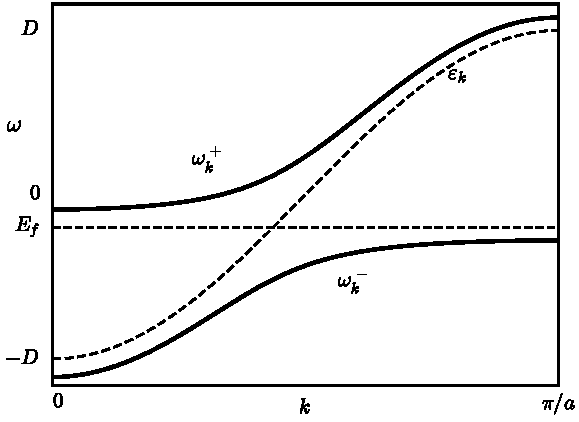
\includegraphics[width=7.5cm]{fig11-15.pdf}\\{\small 图 11.15\quad 重整杂化带的示意图，其中设\\
$\varepsilon_{k}=D\cos(ka)$，$E_{\mathrm{f}}=-0.2D$，$\widetilde{V}^{2}=0.1D$}
\end{minipage}
\end{center}

利用 $B=(\omega-\omega_{k}^{+})(\omega-\omega_{k}^{-})$ 以及 $(\omega-E_{\mathrm{f}})=-(\partial B/\partial\varepsilon_{k})$ 和 $(\omega-\varepsilon_{k})=-(\partial B/\partial E_{\mathrm{f}})$，类似于从式(11.1.50)导出式(11.1.51)的做法，可将c与f电子在k空间的格林函数写成下列标准形式
\begin{equation}
\begin{aligned}
  \langle\langle C_{km}|C_{km}^{+}\rangle\rangle_{\omega}
  &=\frac{A_{k}^{+}}{\omega-\omega_{k}^{-}}+\frac{A_{k}^{-}}{\omega-\omega_{k}^{+}}\\
  \langle\langle f_{km}|f_{km}^{+}\rangle\rangle_{\omega}
  &=\frac{A_{k}^{-}}{\omega-\omega_{k}^{-}}+\frac{A_{k}^{+}}{\omega-\omega_{k}^{+}}
\end{aligned}
\end{equation}
其中
\begin{equation}
  A_{k}^{\pm}=\frac{1}{2}\biggl\{1\pm\frac{(\varepsilon_{k}-E_{\mathrm{f}})}
  {\sqrt{(\varepsilon_{k}-E_{\mathrm{f}})^{2}+4\widetilde{V}^{2}}}\biggr\}
\end{equation}
并有 $A_{k}^{+}+A_{k}^{-}=1$ 关系.

为了便于计算重费密子系统中c电子与f电子的局域态密度(简称c-DOS与f-DOS)，我们将引入下列平均的格点格林函数：
\begin{subequations}
\begin{equation}
  G_{\mathrm{c}}(\omega)\equiv\frac{1}{N}\sum_{l}\langle\langle C_{lm}|C_{lm}^{+}\rangle\rangle_{\omega}
  =\frac{1}{N}\sum_{k}\langle\langle C_{km}|C_{km}^{+}\rangle\rangle_{\omega}
\end{equation}
\begin{equation}
  G_{\mathrm{f}}(\omega)\equiv\frac{1}{N}\sum_{l}\langle\langle f_{lm}|f_{lm}^{+}\rangle\rangle_{\omega}
  =\frac{1}{N}\sum_{k}\langle\langle f_{km}|f_{km}^{+}\rangle\rangle_{\omega}
\end{equation}
\begin{equation}
  G_{\mathrm{cf}}(\omega)\equiv G_{\mathrm{fc}}(\omega)
  =\frac{1}{N}\sum_{k}\langle\langle C_{km}|f_{km}^{+}\rangle\rangle_{\omega}
\end{equation}
\end{subequations}
根据式(11.1.39)，c-DOS 与 f-DOS 可简单地表示为
\begin{subequations}
\begin{equation}
  \rho_{\mathrm{c}}(\omega)=-\frac{1}{\pi}\mathrm{Im}\,G_{\mathrm{c}}(\omega+\mathrm{i}\eta)
\end{equation}
\begin{equation}
  \rho_{\mathrm{f}}(\omega)=-\frac{1}{\pi}\mathrm{Im}\,G_{\mathrm{f}}(\omega+\mathrm{i}\eta)
\end{equation}
\end{subequations}
其中 $\eta=0^{+}$，再利用格林函数解式(11.8.2)，又可将格点的推迟格写成
\begin{subequations}
\begin{equation}
  G_{\mathrm{c}}(\omega+\mathrm{i}\eta)=\frac{1}{N}\sum_{k}
  \biggl[(\omega-\varepsilon_{k})-\frac{\widetilde{V}^{2}}{(\omega-E_{\mathrm{f}})}+\mathrm{i}\eta\biggr]^{-1}
\end{equation}
\begin{equation}
  G_{\mathrm{f}}(\omega+\mathrm{i}\eta)=\frac{\widetilde{V}^{2}}{(\omega-E_{\mathrm{f}}+\mathrm{i}\eta)^{2}}
  G_{\mathrm{c}}(\omega+\mathrm{i}\eta)+\frac{1}{(\omega-E_{\mathrm{f}}+\mathrm{i}\eta)}
\end{equation}
\begin{equation}
  G_{\mathrm{cf}}(\omega+\mathrm{i}\eta)=\frac{\widetilde{V}}{(\omega-E_{\mathrm{f}})}
  G_{\mathrm{c}}(\omega+\mathrm{i}\eta)
\end{equation}
\end{subequations}
将应用于推导 c-DOS 与 f-DOS 的表示式.

\subsection*{2. 局域态密度}

我们将首先介绍重费密子系统中的c-DOS、f-DOS 以及准粒子态密度与未微扰的导带态密度 $\rho_{\mathrm{c}}^{(0)}(\omega)$ 之间的普遍关系式，然后再采用简化的矩形未微扰导带态密度，给出文献中常见的c-DOS 与f-DOS 公式.

在 $G_{\mathrm{c}}(\omega+\mathrm{i}\eta)$ 的表示式(11.8.9a)中取 $\widetilde{V}=0$，再代入 c-DOS 公式(11.8.8)，可求出未微扰的导带电子态密度
\begin{equation}
  \rho_{\mathrm{c}}^{(0)}(\omega)=-\frac{1}{\pi N}\mathrm{Im}\sum_{k}(\omega-\varepsilon_{k}+\mathrm{i}\eta)^{-1}
  =\frac{1}{N}\sum_{k}\delta(\omega-\varepsilon_{k})
\end{equation}
这是独立粒子系统态密度的标准公式，$\rho_{\mathrm{c}}^{(0)}(\omega)$ 的具体表示式由能带 $\varepsilon_{k}$ 决定.计入重整杂化 $(\widetilde{V}=rV)$ 以后的 c-DOS 可将式(11.8.9a)代入式(11.8.8)，得到
\begin{subequations}
\begin{equation}
  \rho_{\mathrm{c}}(\omega)=-\frac{1}{\pi N}\mathrm{Im}\sum_{k}
  \biggl[\biggl(\omega-\frac{\widetilde{V}^{2}}{\omega-E_{\mathrm{f}}}\biggr)-\varepsilon_{k}+\mathrm{i}\eta\biggr]^{-1}
\end{equation}
并与 $\rho_{\mathrm{c}}^{(0)}(\omega)$ 的表示式相比较，求出一般关系式
\begin{equation}
  \rho_{\mathrm{c}}(\omega)=\rho_{\mathrm{c}}^{(0)}\biggl(\omega-\frac{\widetilde{V}^{2}}{\omega-E_{\mathrm{f}}}\biggr)
\end{equation}
\end{subequations}
类似地，计入重整杂化 $\widetilde{V}$ 以后的f-DOS 可根据式(11.8.9b)写为
\begin{subequations}
\begin{equation}
  \rho_{\mathrm{f}}(\omega)=-\frac{1}{\pi}\mathrm{Im}\biggl[
  \frac{\widetilde{V}^{2}}{(\omega-E_{\mathrm{f}}+\mathrm{i}\eta)^{2}}G_{\mathrm{c}}(\omega+\mathrm{i}\eta)
  +\frac{1}{(\omega-E_{\mathrm{f}}+\mathrm{i}\eta)}\biggr]
\end{equation}
经直接复数运算后，可将等式右边写为
\begin{equation*}
\begin{aligned}
  \frac{\widetilde{V}^{2}}{(\omega-E_{\mathrm{f}})^{2}}\biggl[-\frac{1}{\pi}\mathrm{Im}\,G_{\mathrm{c}}(\omega+\mathrm{i}\eta)\biggr]
  &+\frac{1}{N}\sum_{k}\frac{(\omega-\varepsilon_{k})}{[(\omega-\varepsilon_{k})(\omega-E_{\mathrm{f}})-\widetilde{V}^{2}]}\\
  &\times(\omega-E_{\mathrm{f}})\delta(\omega-E_{\mathrm{f}})
\end{aligned}
\end{equation*}
其中的第二项，由于含 $(\omega-E_{\mathrm{f}})\delta(\omega-E_{\mathrm{f}})$ 因子，对求和无贡献.在物理上，这是由于 $(\omega-E_{\mathrm{f}}+\mathrm{i}\eta)^{-1}$ 及 $(\omega-E_{\mathrm{f}}+\mathrm{i}\eta)^{-2}$ 的极点 $\omega=E_{\mathrm{f}}$ 均不在重整杂化带之中(参考图11.15)，其虚部可以略去.因此 f-DOS 的一般表示式为
\begin{equation}
  \rho_{\mathrm{f}}(\omega)=\frac{\widetilde{V}^{2}}{(\omega-E_{\mathrm{f}})^{2}}\rho_{\mathrm{c}}(\omega)
  =\frac{\widetilde{V}^{2}}{(\omega-E_{\mathrm{f}})^{2}}\rho_{\mathrm{c}}^{(0)}
  \biggl(\omega-\frac{\widetilde{V}^{2}}{\omega-E_{\mathrm{f}}}\biggr)
\end{equation}
\end{subequations}
为了简化运算起见，在文献中常取矩形的未微扰导带态密度
\begin{equation}
  \rho_{\mathrm{c}}^{(0)}(\varepsilon)=\frac{1}{2D}\theta(\varepsilon+D)\theta(\varepsilon-D)
  =\begin{cases}
    \dfrac{1}{2D} & (-D<\varepsilon<+D)\\[2mm]
    0 & (|\varepsilon|>D)
  \end{cases}
\end{equation}
其中 $\theta$ 为阶跃函数，导带宽度为2D，$\varepsilon$ 的原点取在未微扰导带的中央.这一简化的矩形态密度相当于将费密面附近朗道费密液体的线性关系 $(\varepsilon_{k}\sim k)$ 拓宽到全导带 $(-D<\varepsilon<+D)$ 范围.这时重整杂化带中的 c-DOS 由
\begin{equation}
  \rho_{\mathrm{c}}(\omega)=\rho_{\mathrm{c}}^{(0)}[\varepsilon(\omega)]
\end{equation}
决定，其中
\begin{equation}
  \varepsilon(\omega)=\omega-\frac{\widetilde{V}^{2}}{(\omega-E_{\mathrm{f}})}
\end{equation}
而 $\varepsilon(\omega)$ 的带边在 $\varepsilon(\omega)=\pm D$ 处，也就是说带边由下列方程
\begin{equation}
  \omega^{2}-(E_{\mathrm{f}}\pm D)\omega-(\widetilde{V}^{2}\mp DE_{\mathrm{f}})=0
\end{equation}
的根决定.由此可求得重整杂化带的带边为
\begin{equation}
\left.\begin{aligned}
  \omega_{\mathrm{a}}&=\frac{1}{2}\bigl\{(E_{\mathrm{f}}-D)-\sqrt{(E_{\mathrm{f}}+D)^{2}+4\widetilde{V}^{2}}\bigr\}\\
  \omega_{\mathrm{b}}&=\frac{1}{2}\bigl\{(E_{\mathrm{f}}+D)-\sqrt{(E_{\mathrm{f}}-D)^{2}+4\widetilde{V}^{2}}\bigr\}\\
  \omega_{\mathrm{c}}&=\frac{1}{2}\bigl\{(E_{\mathrm{f}}-D)+\sqrt{(E_{\mathrm{f}}+D)^{2}+4\widetilde{V}^{2}}\bigr\}\\
  \omega_{\mathrm{d}}&=\frac{1}{2}\bigl\{(E_{\mathrm{f}}+D)+\sqrt{(E_{\mathrm{f}}-D)^{2}+4\widetilde{V}^{2}}\bigr\}
\end{aligned}\right\}
\end{equation}
其中重整杂化带的上、下带 $\omega_{k}^{\pm}$ 分别落在 $\omega_{\mathrm{a}}<\omega_{k}^{-}<\omega_{\mathrm{b}}$ 及 $\omega_{\mathrm{c}}<\omega_{k}^{+}<\omega_{\mathrm{d}}$ 区域中.因此 c-DOS 与f-DOS 均可利用阶跃函数表示为下列解析形式：
\begin{equation}
\left.\begin{aligned}
  \rho_{\mathrm{c}}(\omega)&=\frac{1}{2D}\bigl[\theta(\omega-\omega_{\mathrm{a}})\theta(\omega_{\mathrm{b}}-\omega)
  +\theta(\omega-\omega_{\mathrm{c}})\theta(\omega_{\mathrm{d}}-\omega)\bigr]\\
  \rho_{\mathrm{f}}(\omega)&=\biggl(\frac{1}{2D}\biggr)\frac{\widetilde{V}^{2}}{(\omega-E_{\mathrm{f}})^{2}}
  \bigl[\theta(\omega-\omega_{\mathrm{a}})\theta(\omega_{\mathrm{b}}-\omega)
  +\theta(\omega-\omega_{\mathrm{c}})\theta(\omega_{\mathrm{d}}-\omega)\bigr]
\end{aligned}\right\}
\end{equation}
或者更为明确地写成
\begin{equation}
  \rho_{\mathrm{c}}(\omega)=\begin{cases}
    \dfrac{1}{2D} & (\omega_{\mathrm{a}}<\omega<\omega_{\mathrm{b}}\ \text{及}\ \omega_{\mathrm{c}}<\omega<\omega_{\mathrm{d}}\ \text{或}\ \omega\in\omega_{k}^{\pm})\\[2mm]
    0 & (\text{在杂化带外})
  \end{cases}
\end{equation}
\begin{equation}
  \rho_{\mathrm{f}}(\omega)=\begin{cases}
    \dfrac{1}{2D}\dfrac{\widetilde{V}^{2}}{(\omega-E_{\mathrm{f}})^{2}} & (\omega\in\omega_{k}^{\pm})\\[2.5mm]
    0 & (\text{在杂化带外})
  \end{cases}
\end{equation}
图 11.16 是 $\rho_{\mathrm{c}}(\omega)$ 与 $\rho_{\mathrm{f}}(\omega)$ 的示意图，其中 $\rho_{\mathrm{c}}(\omega)$ 在重整杂化带内仍为常数，但 $\rho_{\mathrm{f}}(\omega)$ 则随 $(\omega-E_{\mathrm{f}})$ 的减小而增大，在靠近能隙处 f-DOS 远远高于c-DOS.当平均每格点的总电子数 $n_{\mathrm{t}}=n_{\mathrm{c}}+n_{\mathrm{f}}<\nu_{\mathrm{f}}$ 时，下带未被填满，化学势$\mu$在下带 $\omega_{k}^{-}$ 之内，系统属于重费密子金属.当 $\mu\in\omega_{k}^{-}$、$n_{\mathrm{t}}=\nu_{\mathrm{f}}$ 时，$n_{\mathrm{t}}N$ 个电子填满下带 $\omega_{k}^{-}$，它与全空的上带 $\omega_{k}^{+}$ 之间还隔着一个杂化所产生的非直接能隙，对应于重费密子半导体或近藤绝缘体.

\begin{center}
\begin{minipage}{6cm}
\centering
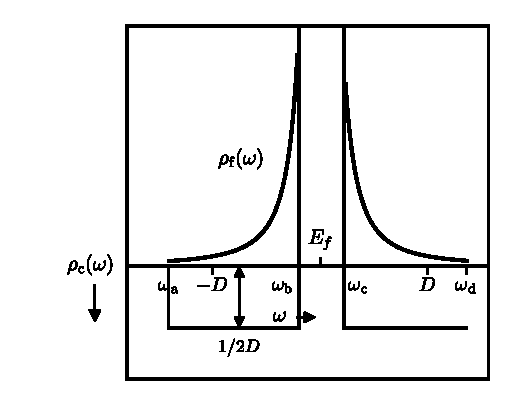
\includegraphics[width=6cm]{fig11-16.pdf}\\{\small 图 11.16\quad f-DOS 和 c-DOS 示意图}
\end{minipage}
\end{center}

重整杂化带的准粒子态密度 $\rho_{\mathrm{QP}}(\omega)$ 与 $\rho_{\mathrm{c}}(\omega)$、$\rho_{\mathrm{f}}(\omega)$ 之间有简单关系.由于 $H_{\mathrm{MF}}$ 可以严格对角化，从格林函数的极点所定出的 $\omega_{k}^{\pm}$ 就是重整杂化能带中的准粒子能量.在平均场近似下，准粒子间无相互作用，它们构成独立电子系统，根据独立粒子系统态密度的基本公式(2.8.7)，任一通道 m的准粒子态密度为
\begin{equation}
  \rho_{\mathrm{QP}}(\omega)=(1/N)\sum_{k}\delta(\omega-\omega_{k}^{-})+(1/N)\sum_{k}\delta(\omega-\omega_{k}^{+})
\end{equation}
另一方面，从c电子与f电子的格林函数表示式(11.8.5)，又可将 c-DOS 与 f-DOS 写成下列形式
\begin{subequations}
\begin{equation}
\begin{aligned}
  \rho_{\mathrm{c}}(\omega)&=-\Bigl(\frac{1}{\pi N}\Bigr)\mathrm{Im}\sum_{k}\biggl\{\frac{A_{k}^{+}}{\omega-\omega_{k}^{-}+\mathrm{i}\eta}
  +\frac{A_{k}^{-}}{\omega-\omega_{k}^{+}+\mathrm{i}\eta}\biggr\}\\
  &=(1/N)\sum_{k}\bigl\{A_{k}^{+}\delta(\omega-\omega_{k}^{-})+A_{k}^{-}\delta(\omega-\omega_{k}^{+})\bigr\}
\end{aligned}
\end{equation}
\begin{equation}
\begin{aligned}
  \rho_{\mathrm{f}}(\omega)&=-\Bigl(\frac{1}{\pi N}\Bigr)\mathrm{Im}\sum_{k}\biggl\{\frac{A_{k}^{-}}{\omega-\omega_{k}^{-}+\mathrm{i}\eta}
  +\frac{A_{k}^{+}}{\omega-\omega_{k}^{+}+\mathrm{i}\eta}\biggr\}\\
  &=\biggl(\frac{1}{N}\biggr)\sum_{k}\bigl\{A_{k}^{-}\delta(\omega-\omega_{k}^{-})+A_{k}^{+}\delta(\omega-\omega_{k}^{+})\bigr\}
\end{aligned}
\end{equation}
\end{subequations}
两式相加，并利用
\begin{equation*}
  A_{k}^{+}+A_{k}^{-}=1
\end{equation*}
立刻得到准粒子态密度式(11.8.21).因此，有关系式
\begin{equation}
  \rho_{\mathrm{QP}}(\omega)=\rho_{\mathrm{c}}(\omega)+\rho_{\mathrm{f}}(\omega)
\end{equation}
说明c与f电子态密度之和即准粒子态密度，用于计算重费密子系统的热力学量.

\subsection*{3. 自洽方程的零温解}

现在讨论自洽方程组式(11.7.29a)与式(11.7.29b)的低温解，目的在于求出隶玻色子平均场参量 $r^{2}(=1-n_{\mathrm{f}})$ 和 $\lambda\ (=E_{\mathrm{f}}-E_{0})$ 的零温解，并讨论系统的属性，用于重费密子金属和近藤绝缘体.

利用格林函数的谱定理
\begin{equation*}
  \langle BA\rangle=\int_{-\infty}^{\infty}\mathrm{d}\omega f(\omega)
  \biggl[-\frac{1}{\pi}\mathrm{Im}\,\langle\langle A|B\rangle\rangle_{\omega+\mathrm{i}\eta}\biggr]
\end{equation*}
和平均的格点格林函数表示式(11.8.9)可将 $r^{2}$ 与λ的自洽方程分别改写为下列表示式.对于 $r^{2}$ 的自洽方程
\begin{equation}
\begin{aligned}
  1-r^{2}=n_{\mathrm{f}}&=\frac{1}{N}\sum_{k,m}\langle f_{km}^{+}f_{km}\rangle_{\mathrm{MF}}\\
  &=\frac{-1}{\pi}\sum_{m}\int_{-\infty}^{\infty}\mathrm{d}\omega f(\omega)\mathrm{Im}
  \biggl\{\frac{1}{N}\sum_{k}\langle\langle f_{km}|f_{km}^{+}\rangle\rangle_{\omega+\mathrm{i}\eta}\biggr\}\\
  &=\nu_{\mathrm{f}}\int_{-\infty}^{\infty}\mathrm{d}\omega f(\omega)
  \biggl\{\biggl(-\frac{1}{\pi}\biggr)\mathrm{Im}\,G_{\mathrm{f}}(\omega+\mathrm{i}\eta)\biggr\}\\
  &=\nu_{\mathrm{f}}\int_{-\infty}^{\infty}\mathrm{d}\omega f(\omega)\rho_{\mathrm{f}}(\omega)
\end{aligned}
\end{equation}
上式表明，任一格点上的平均f电子数 $n_{\mathrm{f}}$ 可直接从 f-DOS 计算.类似的，对于λ的自洽方程
\begin{equation}
\begin{aligned}
  -r\lambda=r(E_{0}-E_{\mathrm{f}})&=\frac{V}{N}\sum_{k,m}\langle f_{km}^{+}C_{km}\rangle_{\mathrm{MF}}\\
  &=\nu_{\mathrm{f}}V\int_{-\infty}^{\infty}\mathrm{d}\omega f(\omega)
  \biggl\{\biggl(-\frac{1}{\pi}\biggr)\mathrm{Im}\,G_{\mathrm{cf}}(\omega+\mathrm{i}\eta)\biggr\}\\
  &=\nu_{\mathrm{f}}V\int_{-\infty}^{\infty}\mathrm{d}\omega f(\omega)\frac{rV}{(\omega-E_{\mathrm{f}})}
  \biggl\{\biggl(-\frac{1}{\pi}\biggr)\mathrm{Im}\,G_{\mathrm{c}}(\omega+\mathrm{i}\eta)\biggr\}\\
  &=\nu_{\mathrm{f}}rV^{2}\int_{-\infty}^{\infty}\mathrm{d}\omega f(\omega)
  \frac{1}{(\omega-E_{\mathrm{f}})}\rho_{\mathrm{c}}(\omega)
\end{aligned}
\end{equation}
再将 $\rho_{\mathrm{c}}$ 与 $\rho_{\mathrm{f}}$ 的具体表示式(11.8.19)与(11.8.20)分别代入上述两式，即可求出 $r^{2}$ 与λ的解.

对于 $n_{\mathrm{t}}<\nu_{\mathrm{f}}$ 的金属情形，化学势 $\boldsymbol{\mu}$ 位于下带 $\omega_{k}^{-}$ 之中，这时 $n_{\mathrm{f}}$ 与 $E_{\mathrm{f}}$（或 $r^{2}$ 与λ)的零温解可以直接求出为
\begin{equation}
  n_{\mathrm{f}}=\frac{\nu_{\mathrm{f}}}{2D}\int_{\omega_{\mathrm{a}}}^{\mu}
  \frac{r^{2}V^{2}}{(\omega-E_{\mathrm{f}})^{2}}\mathrm{d}\omega
  =\frac{\nu_{\mathrm{f}}r^{2}V^{2}}{2D}\biggl\{\frac{1}{(E_{\mathrm{f}}-\mu)}-\frac{1}{(E_{\mathrm{f}}-\omega_{\mathrm{a}})}\biggr\}
\end{equation}
\begin{equation}
  E_{0}-E_{\mathrm{f}}=\frac{\nu_{\mathrm{f}}V^{2}}{2D}\int_{\omega_{\mathrm{a}}}^{\mu}
  \frac{\mathrm{d}\omega}{(\omega-E_{\mathrm{f}})}
  =\frac{\nu_{\mathrm{f}}V^{2}}{2D}\ln\biggl[\frac{(E_{\mathrm{f}}-\mu)}{(E_{\mathrm{f}}-\omega_{\mathrm{a}})}\biggr]
\end{equation}
其中化学势$\mu$由总粒子数 $n_{\mathrm{t}}$ 的守恒条件式(11.7.30)决定，其零温表示式为
\begin{equation}
  n_{\mathrm{t}}=n_{\mathrm{f}}+\nu_{\mathrm{f}}(\mu-\omega_{\mathrm{a}})/2D
\end{equation}
由于强关联将导致f电子局域化，因此在 $U\to\infty$ 时的重整杂化 $\widetilde{V}\ (\widetilde{V}=rV)$ 将比原来的杂化V小得多，再考虑到通常 $V/D<1$，我们有理由认为未微扰的导带半宽度 $D\gg\widetilde{V}$，这时带边值公式(11.8.17)可近似为
\begin{equation}
\left.\begin{aligned}
  \omega_{\mathrm{a}}&\approx-D-r^{2}V^{2}/(D+E_{\mathrm{f}})\\
  \omega_{\mathrm{b}}&\approx E_{\mathrm{f}}-r^{2}V^{2}/(D-E_{\mathrm{f}})\\
  \omega_{\mathrm{c}}&\approx E_{\mathrm{f}}+r^{2}V^{2}/(D+E_{\mathrm{f}})\\
  \omega_{\mathrm{d}}&\approx D+r^{2}V^{2}/(D-E_{\mathrm{f}})
\end{aligned}\right\}
\end{equation}
考虑到 $\omega_{\mathrm{a}}\approx-D$，式(11.8.26)右边的第二项为 $D^{-2}$ 量级可以略去，求得
\begin{equation}
  n_{\mathrm{f}}=1-r^{2}\approx\frac{\nu_{\mathrm{f}}r^{2}V^{2}}{2D(E_{\mathrm{f}}-\mu)}
\end{equation}
上式又可改写为
\begin{equation}
  \frac{E_{\mathrm{f}}-\mu}{D}\approx\biggl(\frac{\nu_{\mathrm{f}}}{2}\biggr)\biggl(\frac{V}{D}\biggr)^{2}\frac{r^{2}}{1-r^{2}}
\end{equation}
显然，$(E_{\mathrm{f}}-\mu)/D$ 是量级为 $r^{2}$ 的小量，在重费密子系统中可以根据 $D\gg\widetilde{V}$ 与 $(E_{\mathrm{f}}-\mu)$ 作近似求出 $n_{\mathrm{f}}$、$E_{\mathrm{f}}$ 及 $\boldsymbol{\mu}$ 的近似表示式.为此，引入下列符号定义
\begin{equation}
  k_{\mathrm{B}}T_{\mathrm{L}}\equiv E_{\mathrm{f}}-\mu,\quad
  \Gamma\equiv\pi V^{2}/2D,\quad
  \widetilde{\Gamma}\equiv\pi r^{2}V^{2}/2D
\end{equation}
其中 $\Gamma$ 代表不计杂化V的重整效应(即取 $r=1$)时安德逊模型中f能级的共振线宽度，与式(11.6.21)中的 $\Gamma$ 是类似的.$T_{\mathrm{L}}$ 是安德逊晶格模型的一个特征温度，$k_{\mathrm{B}}T_{\mathrm{L}}$ 就是从费密面算起的重整f能级.按此，可写出式(11.8.26)—(11.8.28)等3个基本方程的近似表示式
\begin{subequations}
\begin{equation}
  n_{\mathrm{f}}=\nu_{\mathrm{f}}\widetilde{\Gamma}/\pi k_{\mathrm{B}}T_{\mathrm{L}}
  =1-(\widetilde{\Gamma}/\Gamma)=1-r^{2}
\end{equation}
\begin{equation}
  (E_{0}-\mu)-k_{\mathrm{B}}T_{\mathrm{L}}=(\nu_{\mathrm{f}}\Gamma/\pi)\ln[k_{\mathrm{B}}T_{\mathrm{L}}/(D+\mu)]
\end{equation}
\begin{equation}
  n_{\mathrm{t}}=n_{\mathrm{f}}+\nu_{\mathrm{f}}(\mu+D)/2D
\end{equation}
\end{subequations}
从式(11.8.33a)立刻求得 $T=0$ K时
\begin{equation}
  n_{\mathrm{f}}=\frac{1}{1+\pi k_{\mathrm{B}}T_{\mathrm{L}}/\nu_{\mathrm{f}}\Gamma}
\end{equation}
当未微扰的f能级远低于费密能级时，即 $E_{0}-\mu\ll 0$ 并取很大的负值时，可略去式(11.8.33b)左边的 $k_{\mathrm{B}}T_{\mathrm{L}}$ 项，求得特征温度满足
\begin{equation}
  k_{\mathrm{B}}T_{\mathrm{L}}=(D+\mu)\exp\biggl(-\frac{\pi|E_{0}-\mu|}{\nu_{\mathrm{f}}\Gamma}\biggr)
\end{equation}
特别是在近藤极限下，当 $|E_{0}-\mu|\gg\Gamma$ 时，$k_{\mathrm{B}}T_{\mathrm{L}}$ 将比 $(D+\mu)$ 小几个数量级，可以认为式(11.8.34)中的 $(\pi k_{\mathrm{B}}T_{\mathrm{L}}/\nu_{\mathrm{f}}\Gamma)$ 也是一个小参量，展开后求得 $n_{\mathrm{f}}=1-r^{2}\approx 1-(\pi k_{\mathrm{B}}T_{\mathrm{L}}/\nu_{\mathrm{f}}\Gamma)$，其中 $r^{2}\approx(\pi k_{\mathrm{B}}T_{\mathrm{L}}/\nu_{\mathrm{f}}\Gamma)\ll 1$.这时每格点的平均f电子数 $n_{\mathrm{f}}$ 趋近1，但仍然保持为略小于1的近整数，安德逊晶格系统中仍然存在很弱的重整杂化 $\widetilde{V}=rV$（其中 $r^{2}\ll 1$）.因此，人们常将安德逊晶格的近藤极限称为近整数价极限.同时，仍然存在的弱f-c杂化 $\widetilde{V}$，将使f电子成为近局域化的弱巡游电子，导致重费密子特性.

重电子金属中的重费密子特性，在实验上表现为零温比热容系数 $\gamma(0)$ 比普通金属至少高两个量级，在理论上表现为低激发态具有很高的电子有效质量 $(m^{*}/m_{\mathrm{e}})\gg 1$.我们将指出，以上结果均来源于费密面上f电子的态密度 $\rho_{\mathrm{f}}(\mu)$ 远远高于传导电子的态密度 $\rho_{\mathrm{c}}(\mu)$.根据态密度公式(11.8.18)与(11.8.19)可知
\begin{equation}
  \frac{\rho_{\mathrm{f}}(\mu)}{\rho_{\mathrm{c}}(\mu)}=\frac{\widetilde{V}^{2}}{(E_{\mathrm{f}}-\mu)^{2}}
  \approx\biggl(\frac{2}{\nu_{\mathrm{f}}}\biggr)\frac{n_{\mathrm{f}}D}{k_{\mathrm{B}}T_{\mathrm{L}}}\gg 1
\end{equation}
在第二个等式中利用了式(11.8.30)和定义式(11.8.32).显然，在近藤极限可取 $n_{\mathrm{f}}\approx 1$，并设 $\nu_{\mathrm{f}}=2$，则上式右边简化为 $(D/k_{\mathrm{B}}T_{\mathrm{L}})$，因此 $\rho_{\mathrm{f}}(\mu)\gg\rho_{\mathrm{c}}(\mu)$.在固体物理学中已知金属中费密面上任一自旋取向的态密度
\begin{equation}
  \rho(\mu)=\frac{3n}{4E_{\mathrm{F}}}=\frac{m^{*}k_{\mathrm{F}}}{2\pi^{2}h^{2}}
\end{equation}
其中 $m^{*}$ 是电子的有效质量.若取传导电子的有效质量为自由电子质量 $m_{\mathrm{e}}$，并认为重的金属中的高有效质量主要来自f电子，则在近藤极限下取 $\nu_{\mathrm{f}}=2$ 可得
\begin{equation}
  \frac{m^{*}}{m_{\mathrm{e}}}=\frac{\rho_{\mathrm{f}}(\mu)}{\rho_{\mathrm{c}}(\mu)}
  \approx\frac{D}{k_{\mathrm{B}}T_{\mathrm{L}}}\gg 1
\end{equation}
显然，$(E_{\mathrm{f}}-\mu)\equiv k_{\mathrm{B}}T_{\mathrm{L}}$ 取小的正值将导致重费密子效应.从物理角度分析，由于强关联产生的f能级重整化，使f电子从远低于 $\mu$ 的 $E_{0}$ 提升到略高于 $\boldsymbol{\mu}$ 的 $E_{\mathrm{f}}\ (E_{\mathrm{f}}=E_{0}+\lambda)$ 处，并保持 $0<(E_{\mathrm{f}}-\mu)\ll D$，如图11.16所示.从图可知，由于 $E_{\mathrm{f}}$ 位于杂化能隙之中，化学势 $\mu$ 必然落在下带 $\omega_{k}^{-}$ 曲线的平坦变化部分，自然具有很高的准粒子有效质量.

零温时重电子金属的线性比热容系数可从费密面上的准粒子态密度 $\rho_{\mathrm{QP}}(\mu)$ 求出
\begin{equation}
\begin{aligned}
  \gamma(0)&=\nu_{\mathrm{f}}\frac{\pi^{2}k_{\mathrm{B}}^{2}}{3}\rho_{\mathrm{QP}}(\mu)
  =\nu_{\mathrm{f}}\frac{\pi^{2}k_{\mathrm{B}}^{2}}{3}\bigl[\rho_{\mathrm{c}}(\mu)+\rho_{\mathrm{f}}(\mu)\bigr]\\
  &=\nu_{\mathrm{f}}\frac{\pi^{2}k_{\mathrm{B}}^{2}}{3}\biggl[\frac{1}{2D}+\frac{r^{2}V^{2}}{2D(E_{\mathrm{f}}-\mu)^{2}}\biggr]\\
  &=\nu_{\mathrm{f}}\frac{\pi^{2}k_{\mathrm{B}}^{2}}{3}\biggl(\frac{1}{2D}+\frac{n_{f}}{\nu_{\mathrm{f}}k_{\mathrm{B}}T_{\mathrm{L}}}\biggr)
\end{aligned}
\end{equation}
其中利用了式(11.8.30).在普通金属中，由于不存在近局域的f电子，其零温线性比热容系数 $\gamma_{0}(0)$ 可由上式右边第一项表示
\begin{equation}
  \gamma_{0}(0)=\frac{\nu_{\mathrm{f}}\pi^{2}k_{\mathrm{B}}^{2}}{3}\rho_{\mathrm{c}}(\mu)
\end{equation}
当取 $\nu_{\mathrm{f}}=2$ 时，就得到固体物理学中零温比热容系数的标准公式.因此重电子金属与普通金属的零温比热容系数满足下列不等式关系：
\begin{equation}
  \gamma(0)/\gamma_{0}(0)=1+\biggl(\frac{2}{\nu_{\mathrm{f}}}\biggr)\frac{n_{\mathrm{f}}D}{k_{\mathrm{B}}T_{\mathrm{L}}}\gg 1
\end{equation}
与实验观测结果一致.

现在讨论系统的绝缘情形，当 $n_{\mathrm{t}}=\nu_{\mathrm{f}}$ 时准粒子谱的下带从 $\omega_{\mathrm{a}}$ 到 $\omega_{\mathrm{b}}$ 均被填满，上带则是全空的，中间隔着一个杂化能隙 $\Delta=\omega_{\mathrm{c}}-\omega_{\mathrm{b}}$，属于近藤绝缘体.这时可取 $\boldsymbol{\mu}=\boldsymbol{\omega}_{\mathrm{b}}$ 代入化学势方程式(11.8.28)，并利用定义 $(E_{\mathrm{f}}-\mu)\equiv k_{\mathrm{B}}T_{\mathrm{L}}$，可将近藤绝缘体的带边值近似写成下列相对于 $E_{\mathrm{f}}$ 的表示式：
\begin{equation}
\left.\begin{aligned}
  \omega_{\mathrm{a}}&=E_{\mathrm{f}}-2D(1-n_{\mathrm{f}}/\nu_{\mathrm{f}})-k_{\mathrm{B}}T_{\mathrm{L}}\\
  \omega_{\mathrm{b}}&=\mu=E_{\mathrm{f}}-k_{\mathrm{B}}T_{\mathrm{L}}\\
  \omega_{\mathrm{c}}&=E_{\mathrm{f}}+(2n_{\mathrm{f}}/\nu_{\mathrm{f}})k_{\mathrm{B}}T_{\mathrm{L}}\\
  \omega_{\mathrm{d}}&=E_{\mathrm{f}}+(2n_{\mathrm{f}}/\nu_{\mathrm{f}})D+(2n_{\mathrm{f}}/\nu_{\mathrm{f}})k_{\mathrm{B}}T_{\mathrm{L}}
\end{aligned}\right\}
\end{equation}
其中
\begin{equation}
  E_{\mathrm{f}}=D(1-2n_{\mathrm{f}}/\nu_{\mathrm{f}})+(1-2n_{\mathrm{f}}/\nu_{\mathrm{f}})k_{\mathrm{B}}T_{\mathrm{L}}
\end{equation}
在求解式(11.8.27)时，近似取 $E_{\mathrm{f}}-\omega_{\mathrm{a}}=2D(1-n_{\mathrm{f}}/\nu_{\mathrm{f}})$，可将近藤绝缘体的特征温度表示为
\begin{equation}
  k_{\mathrm{B}}T_{\mathrm{L}}=2D(1-n_{\mathrm{f}}/\nu_{\mathrm{f}})
  \exp\biggl(-\frac{\pi|E_{0}-\mu|}{\nu_{\mathrm{f}}\Gamma}\biggr)
\end{equation}
类似于金属情形，近藤绝缘体的特征温度在近藤极限(当 $|E_{0}-\mu|\gg\Gamma$ 时)也是很低的，并满足 $k_{\mathrm{B}}T_{\mathrm{L}}\ll D$ 条件.近藤绝缘体中的能隙 $\Delta$ 可以利用式(11.8.42)写成 $k_{\mathrm{B}}T_{\mathrm{L}}$ 的表示式
\begin{equation}
  \Delta=\omega_{\mathrm{c}}-\omega_{\mathrm{b}}=(1+2n_{\mathrm{f}}/\nu_{\mathrm{f}})k_{\mathrm{B}}T_{\mathrm{L}}
\end{equation}
显然，能隙正比于特征温度，很低的特征温度 $T_{\mathrm{L}}$，将使近藤绝缘体呈现小能隙半导体特征.在 $\mathrm{Ce_{3}Bi_{4}Pt_{3}}$ 等近藤绝缘体材料中，$\Delta$ 只有 meV量级，它很容易因加压、外场和掺杂而改变.此外，从式(11.8.31)还可以看出 $\Delta\approx 2r^{2}V^{2}/D^{2}$，其中 SB 平均场参量 $r^{2}$ 是温度的函数，通过在有限温度解自洽方程式(11.8.24)与(11.8.25)，可求出 $r^{2}(T)$ 随温度升高而减小.因此，近藤绝缘体中的能隙也是温度的函数 $\Delta=\Delta(T)$，并将随升温而消失，使近藤绝缘体过渡为重费密子金属，与实验观测一致.理论上，$\Delta=\Delta(T)$ 来源于多体效应，正是由于费密海中的传导电子与每个元胞中的f电子发生多体杂化效应，使能隙随温度变化，也使近藤绝缘体不同于通常的小能隙半导体，因为后者的能隙不随温度变化.

综上所述，在隶玻色子平均场理论中，存在一个很低的特征温度 $T_{\mathrm{L}}$ 是导致重费密子金属重费密子特性和近藤绝缘体的小能隙半导体特征的共同原因.

\section{t-J模型}

本节主要介绍在强关联极限下如何从单带赫伯德模型导出t-J模型.对适用于描述 $\mathrm{CuO_{2}}$ 平面低激发特征的推广t-J模型及其对铜氧化合物高温超导体的应用也将作定性的讨论.

\subsection*{1. t-J模型的导出}

将单带赫伯德模型写成下列形式
\begin{equation}
  H=-t\sum_{\langle ij\rangle,\sigma}(C_{i\sigma}^{+}C_{j\sigma}+h.c.)
  +U\sum_{i}n_{i\uparrow}n_{i\downarrow}
\end{equation}
相当于在紧束缚近似哈密顿量式(11.1.15)中令 $T_{0}=0$ 和 $|T_{1}|=t$，即取紧束缚近似能带的中央作为能量的原点，$\langle ij\rangle$ 代表最近邻的一对格点 $i$ 与 $j$，并约定对于每个对求和只进行一次，即 $C_{i\sigma}^{+}C_{j\sigma}$ 在约定求和号下仅描述从j向i格点的跃迁.至于从i至j的相反跃迁过程，则由厄米共轭项 $h.c.$ 表示.上式中的 t 又称近邻跃迁能量.当同格点的库仑排斥 $U=0$ 时，系统处于能带极限，所形成的紧束缚近似能带可容纳2N个电子，N为格点数.当每格点的平均电子数 $n=\langle n_{i\uparrow}\rangle+\langle n_{i\downarrow}\rangle=1$ 时，紧束缚近似能带为半满.正因如此，人们将计入库仑关联U项后的 $n=1$ 情形也称为赫伯德模型的半满情形.当 $t=0$ 而 $U\neq 0$ 时，系统处于原子极限.在前面的讨论中已严格证明：这时在任一格点上均有两个非简并的能级，其能级间距为U.当U与t都不为零，且 $(U/t)\gg 1$ 时称为赫伯德模型的强关联极限.在本章的§1“4”中已证明，由于电子在晶格中的跃迁将形成上、下两个子能带，每个子带中只能容纳N个电子，并且两子带中心相距大致为U.

现在讨论 $(U/t)\gg 1$ 和小于半满填充 $(n<1)$ 情形.根据近邻跃迁能量 $t=0$ 时在任一格点i上电子的可能占据情形，将格点i上的占据分为两类：其一是无双占格点态，包括空占据以及自旋朝上和朝下的单占据等3种；其二则是i格点的双占据态，描述同一格点被一对自旋取向相反电子占据的情形.推广到含有N个格点和 $N_{e}$ 个电子 $(N_{e}<N)$ 的晶格系统，设P为将系统投影到不含任何双占格点子空间中的投影算符，而 $Q=1-P$ 将代表另一投影算符，它将系统投影到含有双占格点的子空间.P算符的表示式十分简单
\begin{subequations}
\begin{equation}
  P=\prod_{i=1}^{N}(1-v_{i})\qquad(v_{i}\equiv n_{i\uparrow}n_{i\downarrow})
\end{equation}
显然在P子空间中不存在双占格点态，可简称为无双占子空间.在晶格系统中，Q算符的表示式比较复杂，它可以从下列连乘积的展开求得.设
\begin{equation}
\begin{aligned}
  \prod_{i}(x)&=\prod_{i=1}^{N}\bigl[(1-v_{i})+xv_{i}\bigr]\qquad(0\leqslant x\leqslant 1)\\
  &=P+\sum_{l=1}^{N}x^{l}Q_{l}
\end{aligned}
\end{equation}
其中
\begin{equation}
  Q_{l}=\sum_{(i_{1}\cdots i_{l})}\bigl[v_{i_{1}}\cdots v_{i_{l}}\prod'_{j}(1-v_{j})\bigr]
\end{equation}
代表系统中有l个格点为双占据，$\prod'_{j}$ 则是对 $(i_{1}\cdots i_{l})$ 以外的 $(N-l)$ 个格点的连乘.考虑到 $x=1$ 时的简单关系式 $\prod(1)=1$，可求出满足完备性条件 $P+Q=1$ 的Q表示式
\begin{equation}
  Q=\sum_{l=1}^{N}Q_{l}
\end{equation}
它包括了晶格系统中的所有可能双占情形.投影算符P与Q满足标准运算规律
\begin{equation}
  P^{2}=P,\ Q^{2}=Q,\ PQ=QP=0,\ P+Q=1
\end{equation}
其中还利用了费密子的算符等式
\begin{equation}
  n_{i\sigma}(1-n_{i\sigma})=0\quad\text{或}\quad v_{i}(1-v_{i})=0
\end{equation}
\end{subequations}
在对单带赫伯德模型作正则变换之前，定义
\begin{equation}
  H\equiv T+V,\ T\equiv-t\sum_{\langle ij\rangle,\sigma}(C_{i\sigma}^{+}C_{j\sigma}+h.c.),\
  V\equiv U\sum_{i}n_{i\uparrow}n_{i\downarrow}
\end{equation}
其中 $n_{i\sigma}=C_{i\sigma}^{+}C_{i\sigma}$，利用一个常规恒等式 $C_{i\sigma}=C_{i\sigma}[(1-n_{i\sigma})+n_{i\sigma}]$ 将H中的独立电子运动项 $T$ 直接划分为
\begin{equation}
\begin{aligned}
  T&=-t\sum_{\langle ij\rangle,\sigma}
  \bigl[(1-n_{i\overline{\sigma}})+n_{i\overline{\sigma}}\bigr]C_{i\sigma}^{+}C_{j\sigma}
  \bigl[(1-n_{j\overline{\sigma}})+n_{j\overline{\sigma}}\bigr]\\
  &=T_{\mathrm{h}}+T_{\mathrm{d}}+T_{\mathrm{mix}}
\end{aligned}
\end{equation}
其中
\begin{subequations}
\begin{equation}
  T_{\mathrm{h}}=-t\sum_{\langle ij\rangle,\sigma}(1-n_{i\overline{\sigma}})
  C_{i\sigma}^{+}C_{j\sigma}(1-n_{j\overline{\sigma}})+h.c.
\end{equation}
\begin{equation}
  T_{\mathrm{d}}=-t\sum_{\langle ij\rangle,\sigma}
  n_{i\overline{\sigma}}C_{i\sigma}^{+}C_{j\sigma}n_{j\overline{\sigma}}+h.c.
\end{equation}
\begin{equation}
  T_{\mathrm{mix}}=-t\sum_{\langle ij\rangle,\sigma}\bigl\{(1-n_{i\overline{\sigma}})
  C_{i\sigma}^{+}C_{j\sigma}n_{j\overline{\sigma}}
  +n_{i\overline{\sigma}}C_{i\sigma}^{+}C_{j\sigma}(1-n_{j\overline{\sigma}})+h.c.\bigr\}
\end{equation}
显然，$T_{\mathrm{h}}$代表电子从单占格点j向空占格点i的跃迁，跃迁发生在“下带”之中，描述“下带”中电子通过空占格点的运动项，简称“下带”空穴运动项.$T_{\mathrm{d}}$则是电子从双占格点j向单占格点i的跃迁，它将原来位于“上带”中 $j$ 格点上的第二个电子转移到i格点上，描述“上带”中的双占格点转移.利用式(11.9.2e)—(11.9.2f)易证 $PT_{\mathrm{d}}P=PT_{\mathrm{d}}Q=QT_{\mathrm{d}}P=0$ 和 $T_{\mathrm{d}}=QT_{\mathrm{d}}Q$，表明 $T_{\mathrm{d}}$ 仅出现在含有双占格点的Q子空间中.类似的 $V=U\sum_{i}n_{i\uparrow}n_{i\downarrow}$ 项也是仅仅出现在Q子空间中的项，并有 $V=QVQ$，其它项 $PVP=PVQ=QVP=0$.此外，$T_{\mathrm{mix}}$ 使“上带”与“下带”混合，属于带间跃迁项，正是它联系了“上带”与“下带”的运动.特别是在 $(U/t)\gg 1$ 和 $n<1$ 时，强关联将使“上带”不可能被电子实际占据，但是“上带”作为中间态仍可通过虚激发过程传递强关联效应对“下带”中电子运动的影响.因此 $T_{\mathrm{mix}}$ 项在推导t-J模型时是至关重要的.类似上文的讨论，易证 $PT_{\mathrm{mix}}P=QT_{\mathrm{mix}}Q=0$，再利用 $P+Q=1$ 求出
\begin{equation}
  T_{\mathrm{mix}}=PT_{\mathrm{mix}}Q+QT_{\mathrm{mix}}P=PTQ+QTP
\end{equation}
其中
\begin{equation}
  PT_{\mathrm{mix}}Q=-t\sum_{\langle ij\rangle,\sigma}(1-n_{i\overline{\sigma}})
  C_{i\sigma}^{+}C_{j\sigma}n_{j\overline{\sigma}}+h.c.=PTQ
\end{equation}
\begin{equation}
  QT_{\mathrm{mix}}P=-t\sum_{\langle ij\rangle,\sigma}
  n_{i\overline{\sigma}}C_{i\sigma}^{+}C_{j\sigma}(1-n_{j\overline{\sigma}})+h.c.=QTP
\end{equation}
\end{subequations}
以上结果进一步表明 $T_{\mathrm{mix}}$ 代表电子在两个子空间 P 与 Q之间的跃迁.

为了研究 $T_{\mathrm{mix}}$ 项的影响，再将赫伯德模型改写为
\begin{equation}
\left.\begin{aligned}
  H&=H_{0}+T_{\mathrm{mix}}\\
  H_{0}&=T_{\mathrm{h}}+T_{\mathrm{d}}+V
\end{aligned}\right\}
\end{equation}
注意，现在的 $H_{0}$ 中已包括了库仑关联项 V.利用正则变换式(5.5.8)—(5.5.11)，消去 $T_{\mathrm{mix}}$ 一阶项，求得准至二阶的有效哈密顿量
\begin{equation}
  H_{\mathrm{eff}}=\mathrm{e}^{-S}H\mathrm{e}^{S}=H_{0}+\frac{1}{2}[T_{\mathrm{mix}},S]
\end{equation}
其中变换的母函数 S 必须满足条件
\begin{equation}
  T_{\mathrm{mix}}+[H_{0},S]=0
\end{equation}
对应的矩阵元关系为
\begin{equation}
  (E_{m}-E_{n})\langle m|S|n\rangle=-\langle m|T_{\mathrm{mix}}|n\rangle
\end{equation}
$E_{m}$ 与 $E_{n}$ 分别是 $H_{0}$ 在 $|m\rangle$ 与 $|n\rangle$ 本征态的能量本征值.由此可将 S 写成
\begin{equation}
  S=\sum'_{m,n}|m\rangle\langle m|\frac{T_{\mathrm{mix}}}{(E_{n}-E_{m})}|n\rangle\langle n|
\end{equation}
其中 $|m\rangle\langle m|$ 与 $|n\rangle\langle n|$ 是投影算符的一般记号，它们分别可取 $P\,(Q)$ 与 $Q\ (P)$ 等两种能量本征值不相等的子空间算符，再利用式(11.9.5d)—(11.9.5f)，写出 S 的 P、Q 表示式
\begin{equation}
  S=\frac{PTQ-QTP}{E_{Q}-E_{P}}
\end{equation}
当 $U\gg t$ 时，$H_{0}$ 本征值在上、下子带间的能量差 $E_{Q}-E_{P}\approx U$，其中略去了含t的修正.因此，准至 $T_{\mathrm{mix}}$ 二阶的母函数
\begin{equation}
  S=\frac{PTQ-QTP}{U}
\end{equation}
或者更具体的表示为
\begin{equation}
  S=-(t/U)\sum_{\langle ij\rangle,\sigma}\bigl\{(1-n_{i\overline{\sigma}})C_{i\sigma}^{+}C_{j\sigma}n_{j\overline{\sigma}}
  -n_{i\overline{\sigma}}C_{i\sigma}^{+}C_{j\sigma}(1-n_{j\overline{\sigma}})+h.c.\bigr\}
\end{equation}
这时若将式(11.9.12)和(11.9.5d)代入 $H_{\mathrm{eff}}$ 的表示式(11.9.7)，经简单运算，求出
\begin{equation}
  H_{\mathrm{eff}}=T_{\mathrm{h}}+T_{\mathrm{d}}+V-\frac{1}{U}(PTQ)(QTP)+\frac{1}{U}(QTP)(PTQ)
\end{equation}
但上式仍然代表全希尔伯特空间中的有效哈密顿量，还必须排除双占据将系统限制在P子空间内，因为在强关联 $U\gg t$ 和不超过半满 $(n\leqslant 1)$ 情形，双占据格点实际上不可能出现，系统将被限制在无双占的P子空间中.这时才能求出单带赫伯德模型在强关联极限下描述系统低能激发的等效哈密顿量 $H_{\mathrm{eff}}^{P}$.为此作P投影，并利用 $PQ=QP=0$ 和 $PT_{\mathrm{d}}P=0$ 以及 $PVP=0$ 消去 Q 空间部分
\begin{equation}
  PH_{\mathrm{eff}}P=P\biggl\{T_{\mathrm{h}}-\frac{1}{U}(PTQ)(QTP)\biggr\}P\equiv PH_{\mathrm{eff}}^{P}P
\end{equation}
因此
\begin{equation}
  H_{\mathrm{eff}}^{P}=T_{\mathrm{h}}-\frac{1}{U}(PTQ)(QTP)
\end{equation}
在以后的讨论中略去 $H_{\mathrm{eff}}^{P}$ 的上、下标，简记为H.剩下的工作只是利用式(11.9.5)计算 $(PTQ)(QTP)/U$ 项.运算是直接的，但却较占篇幅，有兴趣的读者可参阅文献[29]，在那里求出了准至两格点求和项的P子空间有效哈密顿量
\begin{equation}
\left.\begin{aligned}
  &H=-t\sum_{\langle ij\rangle,\sigma}(\hat{C}_{i\sigma}^{+}\hat{C}_{j\sigma}+h.c.)
  +J\sum_{\langle i,j\rangle}\biggl(\hat{\boldsymbol{S}}_{i}\cdot\hat{\boldsymbol{S}}_{j}
  -\frac{1}{4}n_{i}n_{j}\biggr)\\
  &\hat{C}_{i\sigma}^{+}=(1-n_{i\overline{\sigma}})C_{i\sigma}^{+},\quad
   \hat{C}_{j\sigma}=C_{j\sigma}(1-n_{j\overline{\sigma}})\\
  &\hat{S}_{i}^{z}=\frac{1}{2}(C_{i\uparrow}^{+}C_{i\uparrow}-C_{i\downarrow}^{+}C_{i\downarrow}),\quad
   \hat{S}_{i}^{+}=C_{i\uparrow}^{+}C_{i\downarrow},\quad
   \hat{S}_{i}^{-}=C_{i\downarrow}^{+}C_{i\uparrow}
\end{aligned}\right\}
\end{equation}
其中 $\boldsymbol{n}_{i}$ 与 $\boldsymbol{n}_{j}$ 分别代表i与j格点的电子数密度算符，$J=(4t^{2}/U)>0$ 描述近邻自旋 $\hat{\boldsymbol{S}}_{i}$ 与 $\hat{\boldsymbol{S}}_{j}$ 之间的反铁磁交换作用.$\hat{C}_{i\sigma}^{+}=(1-n_{i\overline{\sigma}})C_{i\sigma}^{+}$ 与 $\hat{C}_{j\sigma}=C_{j\sigma}(1-n_{j\overline{\sigma}})$ 都是P子空间中的算符，其中要求 $j$ 为单占格点，而i格点应为空占据，H中等式右边第一项就是 $T_{\mathrm{h}}$，它描述电子通过空占格点的跃迁运动.此外，上式中的 $\hat{S}_{i}^{z}$ 与 $\hat{S}_{i}^{\pm}$ 就是人们熟知的自旋1/2算符的费密子表示式(11.6.10).在文献中常利用矢量泡利矩阵 $\hat{\boldsymbol{\sigma}}$，将它们概括为紧凑的矢量表示
\begin{equation}
  \hat{\boldsymbol{S}}_{i}=\frac{1}{2}\sum_{\alpha,\beta}C_{i\alpha}^{+}(\hat{\boldsymbol{\sigma}})_{\alpha\beta}C_{i\beta}
\end{equation}
其中 $\boldsymbol{\alpha}$ 与 $\beta$ 是自旋指标，它们均可取↑或↓，与前面的 $\sigma$ 标相同.式(11.9.7)中的 H 称为t-J模型.因此t-J模型就是单带赫伯德模型的强关联极限.自从高温超导体发现以来，t-J模型一直是研究 $\mathrm{CuO_{2}}$ 平面上二维强关联电子系统的一个重要理论模型.

由于 $T_{\mathrm{h}}$ 是被限制在P子空间中的空穴运动项，其跃迁项中往往涉及4个标准费密算子，将增加具体运算的困难.安德逊认为这一限制的物理机制主要是减小载流子的跃迁概率，可以作近似处理.引入平均每格点上的空穴浓度 $\delta\equiv 1-n$，它描述平均在每个格点上的空穴占据概率.对于 $\hat{C}_{i\sigma}^{+}=(1-n_{i\overline{\sigma}})C_{i\sigma}^{+}$ 可近似用 $\delta C_{i\sigma}^{+}$ 表示，而 $\hat{C}_{j\sigma}=C_{j\sigma}(1-n_{j\overline{\sigma}})$ 则近似用 $nC_{j\sigma}$ 代替，其中 $n=1-\delta$ 代表平均每个格点上电子占据的概率.这样，当系统接近半满$(n\to 1)$时，$\delta$ 很小，在准至 $\delta$ 一阶时可取 $(t\delta)$ 作为有效的跃迁能代替t，并将 $T_{\mathrm{h}}$ 近似用标准费密算子 $C_{i\sigma}^{+}$ 与 $C_{j\sigma}$ 的二次型表示.因此强关联与接近半满填充时t-J模型可写成
\begin{equation}
  H=-(t\delta)\sum_{\langle ij\rangle,\sigma}(C_{i\sigma}^{+}C_{j\sigma}+h.c.)
  +J\sum_{i,j}\biggl(\hat{\boldsymbol{S}}_{i}\cdot\hat{\boldsymbol{S}}_{j}-\frac{1}{4}n_{i}n_{j}\biggr)
\end{equation}
显然，未掺杂时 n = 1 和 $\delta=0$，没有荷电载流子的运动项，H中只剩 $J>0$ 海森伯交换作用项，这时系统的低能激发仅仅以反铁磁自旋波形式出现，即仅有自旋而无电荷自由度的激发.只有经过掺杂，当空穴被引入 $\mathrm{CuO_{2}}$ 平面后，荷电载流子才能在反铁磁背景中运动，这时系统中既有电荷又有自旋自由度，还包括这两种自由度之间的相互竞争.t-J模型以最简洁的形式概括了这一与高温超导体 $\mathrm{CuO_{2}}$ 平面特性密切相关的激发与竞争，使它成为凝聚态物理学中最受关注的模型之一.

\subsection*{2. t-J模型应用于母体化合物}

t-J模型是高温超导研究中的常用理论模型.铜氧化物高温超导体如 $(\mathrm{La}_{1-x}\mathrm{Sr}_{x})_{2}\mathrm{CuO_{4}}$ 系统，用 $\mathrm{Sr}^{2+}$ 离子作为杂质替代 $\mathrm{La}^{3+}$ 离子，将在 $\mathrm{CuO_{2}}$ 平面上引入空穴，当 $\boldsymbol{x}=\boldsymbol{0}$ 时系统是未掺杂的母体化合物La-214(即 $\mathrm{La}_{2}^{3+}\mathrm{Cu}^{2+}\mathrm{O}_{4}^{2-}$).由于 $\mathrm{Cu}^{2+}$ 的电子组态为 $(1\mathrm{s})^{2}\cdots(2\mathrm{p})^{6}\,(3\mathrm{d})^{9}$，其中d壳层是未填满的，因此在 $\mathrm{Cu}^{2+}$ 离子上只有一个自旋未配对的d电子，具有1/2自旋，处于 $3\mathrm{d}_{x^{2}-y^{2}}$ 态.在应用赫伯德模型讨论高温超导体特性时，人们往往不明显地考虑氧离子，而将 $\mathrm{CuO_{2}}$ 平面简单看成是铜离子的二维正方晶格，每个格点上的平均电子数 $n=1$，从理论上讲 $\mathrm{CuO_{2}}$ 平面属于单带赫伯德模型的半满情形.根据赫伯德模型的窄带强关联解，在Cu的二维正方晶格中，N个自旋为1/2的d电子仅填满“下带”，与全空的“上带”之间还被能隙隔开，系统的基态应当是绝缘体，但却不能进一步说明到底是顺磁的，铁磁的，还是反铁磁的绝缘体.铜氧化合物高温超导体的实验结果则进一步证实未掺杂的母体化合物如La-214等都是反铁磁的绝缘体.这一重要实验事实现在可以直接从t-J模型导出.由于此模型的 $H=T_{\mathrm{h}}+$（反铁磁背景项)，其中 $T_{\mathrm{h}}$ 只可能通过最近邻的空占格点跃迁.换句话说，在 $\mathrm{CuO_{2}}$ 平面上必须有空穴才可能出现 $T_{\mathrm{h}}$ 项.在 $U\gg t$ 和严格半满填充 $n=1$ 时，强关联$(U\gg t)$不允许双占格点出现，导致二维晶格中的 N个 d电子必然被N个格点所平分，而在每个格点上总是保持单占据，理论上可以用算符条件 $n_{i}=n_{j}=1$（其中 $n_{i}=n_{i\sigma}+n_{i\overline{\sigma}}$)表示这时 $\hat{C}_{i\sigma}^{+}=(1-n_{i\sigma})C_{i\sigma}^{+}$ 中的 $\sigma$ 自旋态根据泡利原理应为空占据，有 $n_{i\sigma}=0$，但是在取向相反的自旋态 $\overline{\sigma}$ 上，由于又应满足 $n_{i}=1$ 条件，则必须取 $n_{i\overline{\sigma}}=1$ 才能保持i格点在半满时的单占据特征.因此，$T_{\mathrm{h}}$ 中的一般跃迁项 $(1-n_{i\sigma})C_{i\sigma}^{+}C_{j\sigma}(1-n_{j\sigma})$ 在半满情况下必然消失，使 $T_{\mathrm{h}}=0$ 严格成立，其物理原因是由于半满时在 $\mathrm{CuO_{2}}$ 平面中无空穴，将使“下带”中电子无法运动.这样，在半满时t-J模型就直接简化为适用于绝缘磁体的反铁磁海森伯模型
\begin{equation}
  H=J\sum_{\langle ij\rangle}\hat{\boldsymbol{S}}_{i}\cdot\hat{\boldsymbol{S}}_{j}\qquad(J>0)
\end{equation}
其中仅略去了与自旋算符无关的C数项($-J/4$).这个绝缘系统的基态为取向朝上的自旋和取向朝下的自旋在二维正方晶格上交错的排列，朝上自旋的最近邻是朝下的自旋，形成反铁磁长程序，圆满地解释了超导母体化合物是反铁磁绝缘体的实验结果.以上讨论限于未掺杂的 $\boldsymbol{x}=\boldsymbol{0}$ 情形.

当掺杂浓度 $\boldsymbol{x}\neq\boldsymbol{0}$ 时，实验表明，随着x的增加反铁磁奈耳温度 $T_{\mathrm{N}}$ 将迅速下降.\allowbreak 在 $(\mathrm{La}_{1-x}\mathrm{Sr}_{x})_{2}\allowbreak\mathrm{CuO_{4}}$ 中大约 2\%的 Sr掺杂就完全破坏了反铁磁长程序，使 $T_{\mathrm{N}}$ 下降为零.另一方面，实验还证实了掺杂时空穴实际上是进入 $\mathrm{CuO_{2}}$ 平面的氧离子上，表明反铁磁长程序对于在氧离子上出现的空穴十分敏感.基于t-J模型，还可以定性地说明掺杂对于反铁磁序的破坏作用.掺杂后进入 $\mathrm{CuO_{2}}$ 平面中氧位的空穴使氧离子从 $\mathrm{O}^{2-}$ 变为 $\mathrm{O}^{-}$，而且氧空穴 $\mathrm{O}^{-}$ 的自旋与两边的 $\mathrm{Cu}^{2+}$ 自旋也有反铁磁交换作用，其交换作用强度还应当大于 $\mathrm{Cu}^{2+}-\mathrm{Cu}^{2+}$ 之间的反铁磁交换作用强度，因为氧位于两个最近邻铜离子之间，$\mathrm{Cu}^{2+}$ 与 $\mathrm{O}^{-}$ 的间距只是 $\mathrm{Cu}^{2+}-\mathrm{Cu}^{2+}$ 间距的一半.这将使氧空穴 $\mathrm{O}^{-}$ 两边的 $\mathrm{Cu}^{2+}$ 离子自旋取向从原来的反平行变为平行的排列，导致氧空穴周围的 $\mathrm{Cu}^{2+}$ 离子的反铁磁排列失配，从而破坏反铁磁长程序.

根据固体物理学，铜氧平面中的任一格点(或元胞)对应于一个 $\mathrm{CuO_{2}}$ 基元，每个元胞中含有一个Cu原子和两个O原子，共3个离子，构成二维复式晶格.未掺杂时，这些离子分别为 $\mathrm{Cu}^{2+}$ 和 $\mathrm{O}^{2-}$ 状态，其中两个氧离子的最高能级 $2\mathrm{p}_{x}$ 和 $2\mathrm{p}_{y}$ 轨道都已填满，只有 $\mathrm{Cu}^{2+}(3\mathrm{d}^{9}$ 组态)的 $3\mathrm{d}_{x^{2}-y^{2}}$ 轨道为半填满，仅含一个电子并具有自旋1/2.人们似乎可以不明显考虑氧，而把 $\mathrm{CuO_{2}}$ 平面简单看成是 $\mathrm{Cu}^{2+}$ 上电子自旋构成的反铁磁背景.但是，在进一步探索两个 $\mathrm{Cu}^{2+}$ 离子间反铁磁交换作用的成因时，$\mathrm{O}^{2-}$ 离子的中介作用是不可忽略的，下面我们将采用空穴描述对此作定性说明.

在高温超导研究中，人们习惯采用空穴描述，取满壳层的 $3\mathrm{d}^{10}(\mathrm{Cu}^{+})$ 与 $2\mathrm{p}^{6}(\mathrm{O}^{2-})$ 作为系统的真空，这时又可将未掺杂的 $\mathrm{CuO_{2}}$ 平面看成是在每一个格点的 $\mathrm{Cu}^{2+}$ 离子上有一个 $3\mathrm{d}_{x^{2}-y^{2}}$ 空穴并带有自旋，它们构成式(11.9.20)所描述的反铁磁背景，其中 $\hat{\boldsymbol{S}}_{i}$ 现在代表i格点上空穴的自旋算符.相应的在单带赫伯德模型中的 $C_{i\sigma}^{+}(C_{i\sigma})$ 也称作空穴的产生(消灭)算符，而U则是在铜离子上存在一对自旋取向相反的空穴间的库仑排斥.但应注意即使在未掺杂时，$\mathrm{CuO_{2}}$ 平面上的反铁磁交换作用J实际上来源于两个 $\mathrm{Cu}^{2+}$ 离子通过 $\mathrm{O}^{2-}$ 离子的超交换作用.物理上可以用三格点图像定性描述两个 $\mathrm{Cu}^{2+}$（用×表示)的自旋通过与 $\mathrm{O}^{2-}$ 离子（用○表示)之间的多次跃迁，并进行超交换的过程，如图11.17所示\textsuperscript{[30]}.设 $\varepsilon_{\mathrm{d}}$ 与 $\varepsilon_{\mathrm{p}}$ 分别代表Cu（×）与O(○)上空穴的能级，Cu-O 跃迁矩阵元为 $t_{\mathrm{pd}}\ (|t_{\mathrm{pd}}|\equiv t_{0})$，忽略氧上同时出现一对空穴时的库仑作用，只计及铜格点上的库仑关联U.在图11.17中，通道(a)的3个中间态与初态间能量差仅与铜氧间电荷转移能 $\Delta=\varepsilon_{\mathrm{p}}-\varepsilon_{\mathrm{d}}$ 有关.根据四阶微扰，两个 $\mathrm{Cu}^{2+}$ 空穴的自旋交换所降低的能量为 $2(t_{0}^{4}/\Delta^{3})$，出现因子2是由于在(a)通道还有一个等效的过程，其中左边的空穴自旋先向氧转移.类似的，(b)通道也包括两个等价的过程.在(b)中只有一个中间态是铜格点的空穴双占态，它与初态间能量差为U，其它两个中间态仍提供 $\Delta$ 能量差.因此，(b)通道因交换自旋所降低的能量为 $2(t_{0}^{4}/U\Delta^{2})$，这两个通道的贡献之和再乘以2才是在约定求和 $\langle ij\rangle$ 表示中的反铁磁超交换作用

\begin{center}
\begin{minipage}{7cm}
\centering
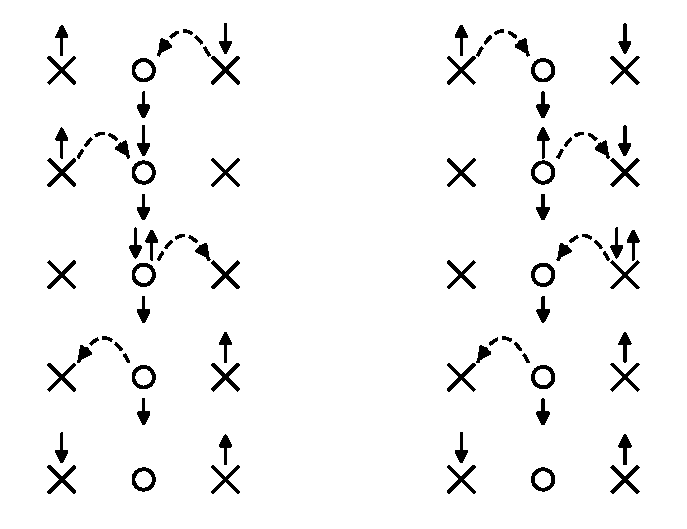
\includegraphics[width=7cm]{fig11-17.pdf}\\{\small (a) 不含U的通道\qquad (b) 含U的通道}\\[3pt]{\small 图 11.17\quad 铜空穴自旋间超交换的两个4阶通道：}
\end{minipage}
\end{center}

\begin{equation}
  J_{\mathrm{eff}}=\frac{4t_{0}^{4}}{\Delta^{2}}\biggl(\frac{1}{\Delta}+\frac{1}{U}\biggr)
  \approx\frac{4(t_{0}^{2}/\Delta)^{2}}{\Delta}
\end{equation}
在后一个等式中采用了近似条件 $U\gg\Delta$，略去(b)通道的贡献.高温超导的实验与理论研究已证明在 $\mathrm{CuO_{2}}$ 层中 $U>\Delta$，称为电荷转移情形，而未掺杂的母体化合物又称电荷转移型的反铁磁绝缘体.以上的定性讨论说明，对于未掺杂的 $\mathrm{CuO_{2}}$ 平面也必须考虑氧离子的作用，只有当超交换作用 $J_{\mathrm{eff}}$ 已求出并用它代替式(11.9.20)中的J以后，才能正确描述铜氧化合物.这时系统等效于半满单带赫伯德模型的强关联极限，其中仍然是 $\mathrm{Cu}^{2+}$ 空穴的自旋所构成的反铁磁背景，氧离子的作用已经包括在 $J_{\mathrm{eff}}$ 之中了.

\subsection*{3. 张-莱斯单态\textsuperscript{[31]}和推广的t-J模型}

在氧化物高温超导体发现的初期安德逊曾假定掺杂后进入 $\mathrm{CuO_{2}}$ 平面的多余空穴主要位于铜上并形成 $\mathrm{Cu}^{3+}$ 离子，物理上相当于多余空穴在 $\mathrm{Cu}^{2+}$ 离子构成的反铁磁背景中运动.正是基于这一假定，他首先提出采用单带赫伯德模型的强关联极限——t-J模型，描述高 $T_{\mathrm{c}}$ 铜氧化合物.但是，实验事实却与安德逊的假定相反，多余的空穴不是位于铜离子上，而是主要位于氧离子上，占据氧的 $2\mathrm{p}_{x}$ 或 $2\mathrm{p}_{y}$ 轨道，并与同一元胞内(或格点i上)的铜 $3\mathrm{d}_{x^{2}-y^{2}}$ 空穴轨道相耦合.单带赫伯德模型，由于未考虑氧离子的作用，已不再是合理的出发模型.人们必须构造一个明显含氧的 $2\mathrm{p}_{x}$、$2\mathrm{p}_{y}$ 和铜的 $3\mathrm{d}_{x^{2}-y^{2}}$ 空穴轨道在内的三带赫伯德模型，并用它描述 $\mathrm{CuO_{2}}$ 平面上的空穴运动才是正确的出发点.当存在多余空穴时，从三带赫伯德模型出发是否仍然可以用一个等效的单带t-J模型描述 $\mathrm{CuO_{2}}$ 平面的低激发特征？这个问题引起了大多数研究者的怀疑.张和莱斯\textsuperscript{[31]}在充分考虑了 Cu-O 杂化和 Cu 离子上强关联效应的情况下，首先证明了在 $\mathrm{CuO_{2}}$ 平面上的一个多余空穴，当它处于 $\mathrm{Cu}^{2+}$ 离子的4个近邻配位氧的对称组合轨道上时，将与此 $\mathrm{Cu}^{2+}$ 离子的 $3\mathrm{d}_{x^{2}-y^{2}}$ 轨道上的空穴之间通过杂化形成局域的单重态，将 $\mathrm{O}^{-}$ 空穴束缚在如图11.18所示的“方块”之中，这个 Cu-O 杂化的单重态被

\begin{center}
\begin{minipage}{6.5cm}
\centering
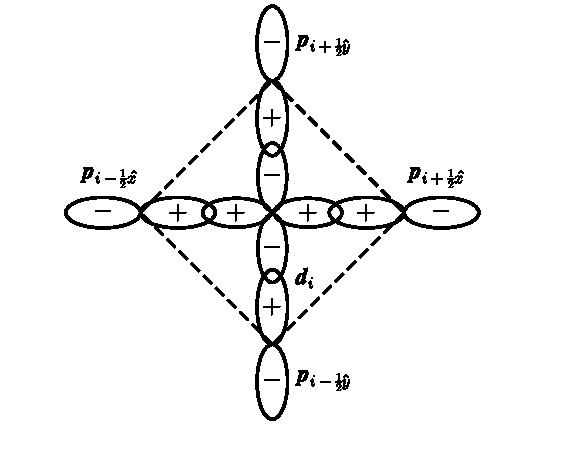
\includegraphics[width=6.5cm]{fig11-18.pdf}\\{\small 图 11.18\quad 氧空穴$(2\mathrm{p}^{5})$与铜空穴$(3\mathrm{d}^{9})$的杂化示意图.图中的“$\pm$”号代表波函数的相位}
\end{minipage}
\end{center}

称作张-莱斯单重态(ZRS).$\mathrm{CuO_{2}}$ 层的低激发态可以用 ZRS 在超交换反铁磁背景中的隧穿运动描述，等效于t-J模型，只是t现在应理解为ZRS在近邻格点间的跃迁能.张-莱斯的工作包括从三带简化为双带，再从双带系统演变为描述 $\mathrm{CuO_{2}}$ 平面低激发特征的等效单带系统.他们从三带模型出发
\begin{equation}
  H=\sum_{i,\sigma}\varepsilon_{\mathrm{d}}d_{i\sigma}^{+}d_{i\sigma}
  +\sum_{l,\sigma}\varepsilon_{\mathrm{p}}p_{l\sigma}^{+}p_{l\sigma}
  +U\sum_{i}n_{i\uparrow}^{d}n_{i\downarrow}^{d}+H'
\end{equation}
其中 $n_{i\sigma}^{d}=d_{i\sigma}^{+}d_{i\sigma}$，$d_{i\sigma}^{+}$ 是i 格点上 Cu 的 $3\mathrm{d}_{x^{2}-y^{2}}$ 空穴的产生算符，U是 Cu 格点的同位库仑排斥，$\varepsilon_{\mathrm{d}}$ 代表 Cu 的 $3\mathrm{d}_{x^{2}-y^{2}}$ 轨道能量.$p_{l\sigma}^{+}$ 表示在l位上O的 $2\mathrm{p}_{x}$ 和 $2\mathrm{p}_{y}$ 空穴的产生算符，可将它们分别写为 $l=i+\frac{1}{2}\hat{x}$ 和 $l=i+\frac{1}{2}\hat{y}$ 代表同一元胞内的两个氧位，$\varepsilon_{\mathrm{p}}$ 是 $2\mathrm{p}_{x}$ 与 $2\mathrm{p}_{y}$ 轨道能量.张和莱斯略去O的同位库仑排斥，O-O和 Cu-Cu 的直接跃迁项，仅考虑距离最近的 Cu-O 跃迁项，如图11.18所示，这时 H'可称作 Cu-O杂化项，并具体写为
\begin{equation}
  H'=t_{0}\sum_{i,\sigma}\biggl\{d_{i\sigma}^{+}\biggl(p_{i-\frac{1}{2}\hat{x},\sigma}
  +p_{i-\frac{1}{2}\hat{y},\sigma}-p_{i+\frac{1}{2}\hat{x},\sigma}
  -p_{i+\frac{1}{2}\hat{y},\sigma}\biggr)+h.c.\biggr\}
\end{equation}
其中 $t_{0}\,(=|t_{\mathrm{pd}}|)$ 代表 Cu-O跃迁矩阵元的数值，它正比于 Cu与O空穴波函数的重叠，此外还应考虑空穴波函数相位的影响.参考图11.18可知，对于 $i-\frac{1}{2}\hat{x}$ 与 $i-\frac{1}{2}\hat{y}$ 是相位一致情形，取$+$号，而 $i+\frac{1}{2}\hat{x}$ 与 $i+\frac{1}{2}\hat{y}$ 则代表相位相反的重叠应取$-$号.这里取 Cu-Cu间距为长度的单位，$\hat{\boldsymbol{x}}$ 与 $\hat{\boldsymbol{y}}$ 分别是x与$y$方向的单位矢量. Cu-O杂化项H'具有重要的对称特征.为了明显看出此特征，定义下列对称化的组合轨道态
\begin{equation}
  P_{i\sigma}=\frac{1}{2}\biggl(p_{i-\frac{1}{2}\hat{x}\sigma}+p_{i-\frac{1}{2}\hat{y}\sigma}
  -p_{i+\frac{1}{2}\hat{x}\sigma}-p_{i+\frac{1}{2}\hat{y}\sigma}\biggr)
\end{equation}
可将Cu-O杂化项，式(11.9.23)，更明确地表示为
\begin{equation}
  H'=2t_{0}\sum_{i,\sigma}(d_{i\sigma}^{+}P_{i\sigma}+h.c.)
\end{equation}
显然，Cu-O杂化仅仅发生在 $\mathrm{Cu}^{2+}$ 的 $3\mathrm{d}_{x^{2}-y^{2}}$ 轨道态与氧的对称组合轨道态 $P_{i\sigma}$ 之间，而且 $P_{i\sigma}$ 态与 $\mathrm{Cu}^{2+}$ 空穴有相同的 $\mathrm{d}_{x^{2}-y^{2}}$ 对称性，如图11.19所示.由于 $P_{i\sigma}$ 只是i元胞内的一种组合态，还应有另一种反对称的组合态 $P_{i\sigma}^{A}=\frac{1}{2}\sum_{l\in i}p_{l\sigma}$，其中l取 $i\pm\frac{1}{2}\hat{x}$ 与 $i\pm\frac{1}{2}\hat{y}$.但是，由于 $P_{i\sigma}^{A}$ 组合与 $\mathrm{Cu}^{2+}$ 离子之间没有杂化，属于O的非成键态，在讨论 $\mathrm{CuO_{2}}$ 面低激发特征时，可以略去无关的非成键态 $P_{i\sigma}^{A}$，而只考虑对称组合态 $P_{i\sigma}$.这样，系统就从原来每个元胞内含有一个

\begin{center}
\begin{minipage}{7cm}
\centering
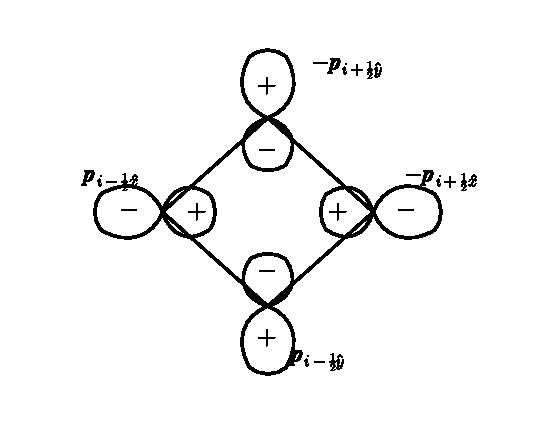
\includegraphics[width=7cm]{fig11-19.pdf}\\{\small 图 11.19\quad 氧空穴的对称组合轨道 $\boldsymbol{P}_{i\sigma}$，其中每个方块内为氧空穴波函数均具有 $\mathrm{d}_{x^{2}-y^{2}}$ 对称性}
\end{minipage}
\end{center}

$\mathrm{Cu}^{2+}$和两个氧 $(2\mathrm{p}_{x}$ 和 $2\mathrm{p}_{y})$ 轨道的三带问题简化为每个元胞中一个 $\mathrm{Cu}^{2+}$ 的 $3\mathrm{d}_{x^{2}-y^{2}}$ 轨道态 $(d_{i\sigma})$ 与一个对称组合轨道态 $(P_{i\sigma})$ 的两带杂化系统.在讨论两带杂化形成张-莱斯单重态之前，还应注意到式(11.9.24)所定义的 $P_{i\sigma}$ 不是标准的费密算子，它满足下列非正交对易关系
\begin{equation}
  \bigl[P_{i\sigma},P_{j\sigma'}^{+}\bigr]_{+}=\delta_{\sigma\sigma'}\biggl(\delta_{ij}-\frac{1}{4}\delta_{\langle ij\rangle>0}\biggr)
\end{equation}
其中仅仅在 $i$ 与j为最近邻格点时，$\delta_{\langle ij\rangle>0}=1$，而在其它情形下都等于零.利用傅里叶变换首先求出在布洛赫表象中满足费密子标准对易式 $[P_{k\sigma},P_{k'\sigma'}^{+}]_{+}=\delta_{\sigma\sigma'}\delta_{kk'}$ 的正则算符
\begin{subequations}
\begin{equation}
  P_{k\sigma}=\frac{1}{\sqrt{N}}\beta_{k}\sum_{i}P_{i\sigma}\exp(-\mathrm{i}\boldsymbol{k}\cdot\boldsymbol{R}_{i})
\end{equation}
\begin{equation}
  \beta_{k}=\biggl[1-\frac{1}{2}(\cos k_{x}+\cos k_{y})\biggr]^{-\frac{1}{2}}
\end{equation}
\end{subequations}
其中 N是 $\mathrm{CuO_{2}}$ 平面上的元胞数，并取晶格常数 $\boldsymbol{a}=\boldsymbol{1}$.再将 $P_{k\sigma}$ 变换到瓦尼尔表象
\begin{subequations}
\begin{equation}
  a_{i\sigma}=\frac{1}{\sqrt{N}}\sum_{k}P_{k\sigma}\exp(\mathrm{i}\boldsymbol{k}\cdot\boldsymbol{R}_{i})
\end{equation}
其中 $\boldsymbol{a}_{i\sigma}$ 满足费密子的标准对易关系
\begin{equation}
  \bigl[a_{i\sigma},a_{j\sigma'}^{+}\bigr]_{+}=\delta_{\sigma\sigma'}\delta_{ij}
\end{equation}
\end{subequations}
上式表明 $a_{i\sigma}$ 是瓦尼尔表象中的标准费密算子，它与非正交的 $P_{i\sigma}$ 算子间的关系可利用逆变换求出为
\begin{subequations}
\begin{equation}
  P_{i\sigma}=\sum_{j}\lambda(\boldsymbol{R}_{i}-\boldsymbol{R}_{j})a_{j\sigma}
\end{equation}
\begin{equation}
  \lambda(\boldsymbol{R}_{i}-\boldsymbol{R}_{j})=\frac{1}{N}\sum_{k}\beta_{k}^{-1}
  \exp[\mathrm{i}\boldsymbol{k}\cdot(\boldsymbol{R}_{i}-\boldsymbol{R}_{j})]
\end{equation}
\end{subequations}
对于二维正方晶格所求得的系数 $\lambda(\boldsymbol{R}_{i}-\boldsymbol{R}_{j})$ 为：当 $\boldsymbol{R}_{i}=\boldsymbol{R}_{j}$ 时取 $\lambda_{0}=0.96$，而当 $\boldsymbol{R}_{j}$ 为 $\boldsymbol{R}_{i}$ 的最近邻 Cu 格点时取 $\lambda_{1}=0.14$，次近邻值 $\lambda_{2}$ 更小，可忽略不计.这时近似用 $a_{i\sigma}+\sum_{j\in(i)}a_{j\sigma}$ 代替 $H'$ 中的 $P_{i\sigma}$ 描述两带杂化系统.在不包括非成键态的子空间中，两带系统的哈密顿量可表示为
\begin{equation}
\begin{aligned}
  H=\sum_{i,\sigma}\varepsilon_{\mathrm{d}}d_{i\sigma}^{+}d_{i\sigma}
  &+U\sum_{i}n_{i\uparrow}^{d}n_{i\downarrow}^{d}
  +\sum_{i,\sigma}\varepsilon_{\mathrm{p}}a_{i\sigma}^{+}a_{i\sigma}\\
  &+2\lambda_{0}t_{0}\sum_{i,\sigma}(d_{i\sigma}^{+}a_{i\sigma}+a_{i\sigma}^{+}d_{i\sigma})
  +2\lambda_{1}t_{0}\sum_{i,\sigma}\sum_{j\in(i)}(d_{i\sigma}^{+}a_{j\sigma}+a_{j\sigma}^{+}d_{i\sigma})
\end{aligned}
\end{equation}
其中 $a_{i\sigma}$ 是描述对称组合氧轨道上多余空穴的标准费密算子，其波函数 $a_{i\sigma}$ 具有与 $\mathrm{Cu}^{2+}$ 空穴波函数相同的 $\mathrm{d}_{x^{2}-y^{2}}$ 对称性.根据量子力学，$\boldsymbol{a}_{i\sigma}$ 上的多余空穴由于与 $\mathrm{Cu}^{2+}$ 空穴的波函数重叠大，而且相位相干(即是两个波函数的相同相位叠加)，必然有利于将此多余空穴束缚在如图11.18所示的方块之中，并与 $\mathrm{Cu}^{2+}$ 的 $3\mathrm{d}_{x^{2}-y^{2}}$ 空穴形成一个局域的自旋单重态
\begin{equation}
  b_{i}^{+}=(a_{i\uparrow}^{+}d_{i\downarrow}^{+}-a_{i\downarrow}^{+}d_{i\uparrow}^{+})/\sqrt{2}
\end{equation}
称为张-莱斯单重态.尽管也可能存在 Cu 与O空穴的自旋三重态，但却不能形成局域束缚态，其能量将比局域的自旋单重态高很多，与氢分子中的情况相似.张和莱斯的微扰估计表明：由于相位相干效应，使能量最低的自旋单重态和自旋三重态之间存在较大的能量间距，它比自旋单重态在反铁磁背景中的近邻跃迁能要高得多.因此，可以忽略单重态与三重态之间的跃迁，将系统限制在只含 Cu-O 杂化单重态的子空间之中.在前面的讨论中已经指出，在强关联情况下单占据的 $\mathrm{Cu}^{2+}$ 空穴构成超交换作用的反铁磁背景，而限制在单重态子空间中的系统在强关联极限也就自然地演变为ZRS在反铁磁背景中的隧穿运动问题，这就是张和莱斯论证系统从双带演变为有效单带的物理内容.ZRS在近邻元胞 i与j之间的隧穿能可利用式(11.9.30)中的两个 Cu-O 杂化项作微扰估计.这是一个包括 $\lambda_{0}t_{0}$（同元胞)和 $\lambda_{1}t_{0}$（近邻元胞)杂化的两步 Cu-O 是跃迁过程，其二阶跃迁矩阵元大致为 $-8\lambda_{0}\lambda_{1}(t_{0}^{2}/\Delta)\approx-(t_{0}^{2}/\Delta)$，其中包括了 Cu 与O空穴之间的自旋交换(即i元胞内的 $\mathrm{Cu}^{2+}$ 空穴通过 $\lambda_{1}t_{0}$ 杂化项跃迁到 j 元胞的氧轨道上，与此同时 i 元胞内的氧空穴因 $\lambda_{0}t_{0}$ 项作用向同元胞内的 Cu 位跃迁等过程).这样才能保证，在反铁磁背景中，跃迁后的近邻 j 元胞中也形成自旋单重态.最后，我们将说明张-莱斯的一个主要论点：在反铁磁背景中的一个局域自旋单重态(即ZRS)等效于在t-J模型中的一个空占格点态.这是因为当在i元胞内存在 ZRS 时，$\mathrm{Cu}^{2+}$ 背景中原有空穴的自旋将被O轨道上的多余空穴所屏蔽，形成总自旋为零的单态，而且是元胞(方块)范围内的局域自旋单态，将导致ZRS不再与其它元胞内的d空穴发生磁互作用.从不明显考虑氧位的观点看，可以认为一个ZRS相当于在 i 元胞内的一个等效的“安德逊 $\mathrm{Cu}^{3+}$ 态.”这时 $\mathrm{CuO_{2}}$ 层的低激发特征可以用一个类似于式(11.9.17)的推广的t-J模型描述
\begin{subequations}
\begin{equation}
\begin{aligned}
  H_{\mathrm{eff}}&=-t_{\mathrm{eff}}\sum_{\langle ij\rangle,\sigma}\bigl\{(1-n_{i\overline{\sigma}})
  C_{i\sigma}^{+}C_{j\sigma}(1-n_{j\overline{\sigma}})+h.c.\bigr\}\\
  &\quad+J_{\mathrm{eff}}\sum_{\langle ij\rangle}\biggl(\hat{\boldsymbol{S}}_{i}\cdot\hat{\boldsymbol{S}}_{j}
  -\frac{1}{4}\boldsymbol{n}_{i}\boldsymbol{n}_{j}\biggr)
\end{aligned}
\end{equation}
其中
\begin{equation}
  t_{\mathrm{eff}}=(t_{0}^{2}/\Delta),\ J_{\mathrm{eff}}=(4t_{\mathrm{eff}}^{2}/\Delta),\ \Delta=\varepsilon_{\mathrm{p}}-\varepsilon_{\mathrm{d}}
\end{equation}
\end{subequations}
为了与前文中t-J模型的符号一致.在上式中已用 $C_{j\sigma}$ 与 $C_{i\sigma}^{+}$ 代替 $d_{j\sigma}$ 与 $d_{i\sigma}^{+}$.从以上介绍可知，张-莱斯的工作主要是物理推论，而不是严格的数学证明.如何从三带赫伯德模型出发，经严格的正则变换，直接导出强关联极限下的等效t-J模型，至今尚无定论.但是ZRS概念已经为多数研究者所接受，并且在掺杂 La-214 中的 X射线吸收谱测量\textsuperscript{[32]}也支持他们关于存在 Cu-O 杂化的单重态和三重态的物理推论.张和莱斯在1988年完成的这篇短文，由于物理内涵丰富，受到超导理论研究者的普遍关注，并具有很高的引用率.

\section{高温超导体的平均场理论}

本节将从推广的t-J模型出发，在平均场近似下讨论高温超导体的d波配对和正常态能隙特征.为简单起见，将式(11.9.32)中的 $t_{\mathrm{eff}}$ 与 $J_{\mathrm{eff}}$ 仍用t 与 J表示
\begin{equation}
  H=T_{\mathrm{h}}+H_{\mathrm{J}}=-t\sum_{\langle ij\rangle,\sigma}(\hat{C}_{i\sigma}^{+}\hat{C}_{j\sigma}+h.c.)
  +J\sum_{\langle ij\rangle}\biggl(\hat{\boldsymbol{S}}_{i}\cdot\hat{\boldsymbol{S}}_{j}
  -\frac{1}{4}n_{i}n_{j}\biggr)
\end{equation}
其中 $\hat{C}_{i\sigma}$ 和 $\hat{C}_{j\sigma}^{+}$ 就是本章§7中的赫伯德投影算符[参见式(11.7.9)的附注]
\begin{subequations}
\begin{equation}
  \hat{C}_{i\sigma}^{+}=(1-n_{i\overline{\sigma}})C_{i\sigma}^{+},\quad
  \hat{C}_{j\sigma}=C_{j\sigma}(1-n_{j\overline{\sigma}})
\end{equation}
利用强关联极限下的无双占格点条件 $n_{i\uparrow}n_{i\downarrow}=0$，我们又可以用 $\hat{C}_{i\sigma}$ 与 $\hat{C}_{i\sigma}^{+}$ 代替式(11.9.18)中的 $C_{i\sigma}$ 与 $C_{i\sigma}^{+}$，将自旋1/2算符的矢量表示式写为
\begin{equation}
  \hat{\boldsymbol{S}}_{i}=\frac{1}{2}\sum_{\alpha,\beta}\hat{C}_{i\alpha}^{+}(\hat{\boldsymbol{\sigma}})_{\alpha\beta}\hat{C}_{i\beta}
\end{equation}
\end{subequations}
再利用等式
\begin{equation}
  (\hat{\boldsymbol{\sigma}})_{\alpha\beta}\bullet(\hat{\boldsymbol{\sigma}})_{\mu\nu}
  =2\delta_{\alpha\nu}\delta_{\beta\mu}-\delta_{\alpha\beta}\delta_{\mu\nu}
\end{equation}
可将反铁磁超交换作用项 $H_{\mathrm{J}}$ 改写成赫伯德投影算符的表示式
\begin{subequations}
\begin{equation}
\begin{aligned}
  H_{\mathrm{J}}&=J\sum_{\langle ij\rangle}\biggl(\hat{\boldsymbol{S}}_{i}\cdot\hat{\boldsymbol{S}}_{j}
  -\frac{1}{4}n_{i}n_{j}\biggr)\\
  &=(-J/2)\sum_{\langle ij\rangle,\sigma}
  (\hat{C}_{i\sigma}^{+}\hat{C}_{j\overline{\sigma}}^{+}\hat{C}_{j\overline{\sigma}}\hat{C}_{i\sigma}
  +\hat{C}_{i\sigma}^{+}\hat{C}_{j\overline{\sigma}}^{+}\hat{C}_{i\overline{\sigma}}\hat{C}_{j\sigma})
\end{aligned}
\end{equation}
而描述“下带”中空穴运动项的 $T_{\mathrm{h}}$ 项则直接写为
\begin{equation}
  T_{\mathrm{h}}=-t\sum_{\langle ij\rangle,\sigma}(\hat{C}_{i\sigma}^{+}\hat{C}_{j\sigma}+h.c.)
\end{equation}
\end{subequations}
这时采用隶玻色子技巧处理赫伯德投影算符 $\hat{C}_{i\sigma}$ 与 $\hat{C}_{i\sigma}^{+}$，将便于在平均场近似下进行解析研究.巴斯卡让(Baskaran)、邹(Zou)和安德逊\textsuperscript{[33]}首先建立了t-J模型的隶玻色子平均场近似理论.类似于式(11.7.13)，将投影算符 $\hat{C}_{i\sigma}^{+}(\hat{C}_{i\sigma})$ 写成标准费密算子 $f_{i\sigma}^{+}(f_{i\sigma})$ 与隶玻色子算子 $b_{i}\ (b_{i}^{+})$ 的双线性乘积：
\begin{subequations}
\begin{equation}
  \hat{C}_{i\sigma}^{+}=b_{i}f_{i\sigma}^{+},\quad \hat{C}_{i\sigma}=f_{i\sigma}b_{i}^{+}
\end{equation}
并满足类似于式(11.7.12)的强关联约束条件
\begin{equation}
  b_{i}^{+}b_{i}+\sum_{\sigma}f_{i\sigma}^{+}f_{i\sigma}=1
\end{equation}
\end{subequations}
根据他们(BZA)的观点，描述 $\mathrm{CuO_{2}}$ 平面上空占格点态的隶玻色子算子 $b_{i}$ 与 $b_{i}^{+}$ 应理解为带有电荷但无自旋的玻色子，称为空穴子，而 $f_{i\sigma}$ 与 $f_{i\sigma}^{+}$ 则描述带有1/2自旋但无电荷的费密子，又称自旋子(spinon).换句话说，是用空穴子与自旋子分别描述物理粒子的电荷与自旋自由度.

隶玻色子表示中的 $T_{\mathrm{h}}$ 与 $H_{\mathrm{J}}$ 分别为
\begin{subequations}
\begin{equation}
  T_{\mathrm{h}}=-t\sum_{\langle ij\rangle,\sigma}(b_{j}^{+}b_{i}f_{i\sigma}^{+}f_{j\sigma}+h.c.)
\end{equation}
\begin{equation}
  H_{\mathrm{J}}=-(J/2)\sum_{\langle ij\rangle,\sigma}
  \bigl(f_{i\sigma}^{+}f_{j\overline{\sigma}}^{+}f_{j\overline{\sigma}}f_{i\sigma}
  +f_{i\sigma}^{+}f_{j\overline{\sigma}}^{+}f_{i\overline{\sigma}}f_{j\sigma}\bigr)
\end{equation}
\end{subequations}
在式(11.10.6b)中本来还应有乘子 $(1+b_{i}^{+}b_{i})(1+b_{j}^{+}b_{j})$ 出现.考虑到 $\boldsymbol{\delta}=1-n$，其中 $n=\sum_{\sigma}\langle f_{i\sigma}^{+}f_{i\sigma}\rangle$，再利用约束条件的平均，有 $\langle b_{i}^{+}b_{i}\rangle=\langle b_{j}^{+}b_{j}\rangle=\delta$.当系统接近半满时，$\delta$ 只是一个小量，这时可以略去 $\boldsymbol{\delta}$ 将上述乘子近似为1.计入约束条件式(11.10.5b)和化学势 $\boldsymbol{\mu}$ 项，将隶玻色子表示中的总哈密顿量写为
\begin{equation}
  \mathscr{H}=T_{\mathrm{h}}+H_{\mathrm{J}}-\mu\sum_{i,\sigma}f_{i\sigma}^{+}f_{i\sigma}
  +\sum_{i}\lambda_{i}\biggl(b_{i}^{+}b_{i}+\sum_{\sigma}f_{i\sigma}^{+}f_{i\sigma}-1\biggr)
\end{equation}
在上式中的 $H_{\mathrm{J}}$ 还可以改写成另一种表示式
\begin{subequations}
\begin{equation}
  H_{\mathrm{J}}=-J\sum_{\langle ij\rangle}b_{ij}^{+}b_{ij}
\end{equation}
其中
\begin{equation}
  b_{ij}^{+}\equiv(f_{i\uparrow}^{+}f_{j\downarrow}^{+}-f_{i\downarrow}^{+}f_{j\uparrow}^{+})/\sqrt{2},\quad
  b_{ij}\equiv(f_{j\downarrow}f_{i\uparrow}-f_{j\uparrow}f_{i\downarrow})/\sqrt{2}
\end{equation}
\end{subequations}
代表近邻格点之间自旋子的单重态配对算符，描述产生或消灭一个价键态，而 $H_{\mathrm{J}}$ 中则包括了所有可能的近邻价键的组态，所对应的状态在量子力学中应由各种价键组态的线性组合描述，被安德逊称之为共振价键状态.根据 $b_{ij}$ 的定义式可知，在价键态中近邻格点i与j上的自旋取向是不固定的，因此共振价键状态不同于反铁磁奈耳态，它是一种没有长程序的自旋液体态.在 $H_{\mathrm{J}}$ 的表示式(11.10.8a)中出现($-$ J)因子也表明形成共振价键状态在能量上是有利的.特别是当 $\mathrm{CuO_{2}}$ 平面上存在掺杂、无序和电子-声子相互作用时，均可能有利于二维正方晶格系统中出现自旋排列的组错，从而导致共振价键状态比反铁磁奈耳态的能量更低，这就是安德逊提出从共振价键状态出发研究高温超导电性机制的主要理由.

\subsection*{1. 平均场近似解和自洽方程}

在作平均场近似时，首先设拉氏乘子 $\lambda_{i}$ 与格点位置无关 $(\lambda_{i}=\lambda)$.在物理上相当于用一个平均约束条件 $\langle b_{i}^{+}b_{i}\rangle+\sum_{\sigma}\langle f_{i\sigma}^{+}f_{i\sigma}\rangle=1$ 代替严格约束条件式(11.10.5b).在对 $T_{\mathrm{h}}$ 与 $H_{\mathrm{J}}$ 项作平均场近似处理时，需定义各类序参量，其中包括描述共振价键态的平均场参量
\begin{subequations}
\begin{equation}
  \Delta_{ij}\equiv\sqrt{2}\,\langle b_{ij}\rangle=
  \begin{cases}
    \Delta_{x} & (j=i\pm\hat{x})\\
    \Delta_{y} & (j=i\pm\hat{y})
  \end{cases}
\end{equation}
其中假定了共振价键序参量与格点i无关，只与近邻格点 i、j 间的取向有关.这里仍取二维正方晶格的元胞边长为长度的单位，$\hat{\boldsymbol{x}}$ 与 $\hat{\boldsymbol{y}}$ 分别代表x与 $y$ 方向的单位矢.再定义
\begin{equation}
  p\equiv\sum_{\sigma}\langle f_{i\sigma}^{+}f_{j\sigma}\rangle=2\langle f_{i\sigma}^{+}f_{j\sigma}\rangle
\end{equation}
\begin{equation}
  q\equiv\langle b_{j}^{+}b_{i}\rangle
\end{equation}
\end{subequations}
并设它们与格点位置、近邻格点间方向以及自旋的取向均无关，由于平均场近似使 $b_{j}^{+}b_{i}f_{i\sigma}^{+}f_{j\sigma}$ 演变为 $qf_{i\sigma}^{+}f_{j\sigma}+(p/2)b_{j}^{+}b_{i}$，可以认为 $\boldsymbol{q}$ 与 $\boldsymbol{p}$ 是描述空穴子与自旋子运动之间相互影响的平均场参量.在完成平均场近似处理后，再作傅里叶变换，最后求得t-J模型的平均场哈密顿量
\begin{equation}
\begin{aligned}
  \mathscr{H}&=\sum_{k,\sigma}\epsilon_{k}f_{k\sigma}^{+}f_{k\sigma}+\sum_{k}\omega_{k}b_{k}^{+}b_{k}
  -\sum_{k}(\Delta_{k}f_{k\uparrow}^{+}f_{-k\downarrow}^{+}+h.c.)\\
  &\quad+N\biggl(4tpq+Jp^{2}+\frac{1}{2}J\Delta_{x}^{2}+\frac{1}{2}J\Delta_{y}^{2}\biggr)
\end{aligned}
\end{equation}
其中
\begin{subequations}
\begin{equation}
  \varepsilon_{k}=-(2tq+Jp)\gamma_{k}-\mu_{f}
\end{equation}
\begin{equation}
  \omega_{k}=-2tp(\gamma_{k}-\gamma_{0})-\mu_{b}
\end{equation}
\begin{equation}
  \Delta_{k}=\sqrt{2}J(\Delta_{x}\cos k_{x}+\Delta_{y}\cos k_{y})
\end{equation}
\end{subequations}
此外，$\mu_{f}=\mu+2J(1-\delta)-\lambda$，$\mu_{b}=-\lambda-2tp\gamma_{0}$ 以及 $\gamma_{k}=\cos k_{x}+\cos k_{y}$.由于哈密顿量式(11.10.10)已简化为二次型，我们可以利用 $u\sim v$ 变换
\begin{equation}
\left.\begin{aligned}
  &f_{k\uparrow}=u_{k}^{*}\alpha_{k}+v_{k}\beta_{-k}^{+},\quad
   f_{-k\downarrow}=u_{k}^{*}\beta_{k}-v_{k}\alpha_{k}^{+}\\
  &|u_{k}|^{2}+|v_{k}|^{2}=1
\end{aligned}\right\}
\end{equation}
将 $\mathscr{H}$ 严格对角化，并得到
\begin{subequations}
\begin{equation}
\begin{aligned}
  \mathscr{H}&=\sum_{k}E_{k}(\alpha_{k}^{+}\alpha_{k}+\beta_{k}^{+}\beta_{k})
  +\sum_{k}\omega_{k}b_{k}^{+}b_{k}+\sum_{k}(\varepsilon_{k}-E_{k})\\
  &\quad+N\biggl(4tp\Delta_{b}+Jp^{2}+\frac{1}{2}J\Delta_{x}^{2}+\frac{1}{2}J\Delta_{y}^{2}\biggr)
\end{aligned}
\end{equation}
\begin{equation}
  E_{k}=\sqrt{\varepsilon_{k}^{2}+\Delta_{k}^{2}}
\end{equation}
\end{subequations}
利用公式 $G(T)=-k_{\mathrm{B}}T\ln\mathrm{Tr}(\mathrm{e}^{-\beta\mathscr{H}})$，不难求出 MFA 的吉布斯自由能
\begin{equation}
\begin{aligned}
  G(T)&=N\biggl(4tp\Delta_{b}+Jp^{2}+\frac{1}{2}J\Delta_{x}^{2}+\frac{1}{2}J\Delta_{y}^{2}\biggr)
  +\sum_{k}\varepsilon_{k}-\\
  &\quad 2k_{\mathrm{B}}T\sum_{k}\ln\bigl[2\cosh(E_{k}/2k_{\mathrm{B}}T)\bigr]
  +k_{\mathrm{B}}T\sum_{k}\ln(1-\mathrm{e}^{-\omega_{k}/k_{\mathrm{B}}T})
  +k_{\mathrm{B}}T\sum_{k}\ln\bigl[2\mathrm{e}^{-\omega_{k}/k_{\mathrm{B}}T}\bigr]
\end{aligned}
\end{equation}
根据吉布斯自由能 $G(T)$ 对 $\Delta_{\alpha}\ (\alpha=x,y)$，$\boldsymbol{q}$ 和 $\boldsymbol{p}$ 的变分极值，不难求得下列自洽方程：
\begin{subequations}
\begin{equation}
  \Delta_{\alpha}=\frac{2J}{N}\sum_{k}\Delta_{k}\cos k_{\alpha}\frac{\tanh(E_{k}/2k_{\mathrm{B}}T)}{E_{k}}
  \qquad(\alpha=x,y)
\end{equation}
\begin{equation}
  q=\frac{1}{2N}\sum_{k}\frac{\gamma_{k}}{\exp(\omega_{k}/k_{\mathrm{B}}T)-1}
\end{equation}
\begin{equation}
  p=\frac{1}{2N}\sum_{k}\gamma_{k}\biggl[1-\frac{\varepsilon_{k}}{E_{k}}\tanh\biggl(\frac{E_{k}}{2k_{\mathrm{B}}T}\biggr)\biggr]
\end{equation}
化学势 $\boldsymbol{\mu}$ 以及λ可利用 $n=(N_{e}/N)=-\dfrac{1}{N}\biggl(\dfrac{\partial G}{\partial\mu}\biggr)$ 和G对λ的变分极值求出
\begin{equation}
  1-\delta=\frac{1}{N}\sum_{k}\biggl[1-\frac{\varepsilon_{k}}{E_{k}}\tanh(E_{k}/2k_{\mathrm{B}}T)\biggr]=n
\end{equation}
\begin{equation}
  \delta=\frac{1}{N}\sum_{k}\ [\exp(\omega_{k}/k_{\mathrm{B}}T)-1]^{-1}
  =\frac{1}{N}\sum_{k}\ \langle b_{k}^{+}b_{k}\rangle
\end{equation}
\end{subequations}
它们是确定 $\boldsymbol{\mu}$ 与λ的自洽方程，实际上就是有限温度时的平均约束条件 $(1/N)\sum_{k}\langle b_{k}^{+}b_{k}\rangle+n=1$，其中 $n=(1/N)\sum_{k,\sigma}\langle f_{k\sigma}^{+}f_{k\sigma}\rangle=(1/N)\sum_{i,\sigma}\langle f_{i\sigma}^{+}f_{i\sigma}\rangle$.

\subsection*{2. d波配对与正常态存在能隙特征}

现在进一步讨论自旋子单重态配对序参量 $\Delta_{\alpha}\ (\alpha=x,y)$ 的自洽方程，在这里仅讨论下列两种情形.

\subsection*{(i) 推广的 s 波情形}

当 $\Delta_{x}=\Delta_{y}=\Delta_{\mathrm{es}}$ 时，式(11.10.15a)可表示为
\begin{subequations}
\begin{equation}
  1=(J/N)\sum_{k}(\gamma_{k}^{2}/E_{k})\tanh(E_{k}/2k_{\mathrm{B}}T)
\end{equation}
其零温自洽方程满足
\begin{equation}
\left.\begin{aligned}
  &1=\frac{J}{N}\sum_{k<k_{\mathrm{F}}}\frac{\gamma_{k}^{2}}{\sqrt{\varepsilon_{k}^{2}+(\sqrt{2}J\gamma_{k}\Delta_{\mathrm{es}})^{2}}}\\
  &\gamma_{k}=\cos k_{x}+\cos k_{y}
\end{aligned}\right\}
\end{equation}
\end{subequations}

\subsection*{(ii) d 波情形}

当 $\Delta_{x}=-\Delta_{y}\equiv\Delta_{\mathrm{d}}$ 时，从式(11.10.15a)将得到
\begin{subequations}
\begin{equation}
  1=(J/N)\sum_{k}(\eta_{k}^{2}/E_{k})\tanh(E_{k}/2k_{\mathrm{B}}T)
\end{equation}
而 $T=0$ K 时的 d 波自洽方程为
\begin{equation}
\left.\begin{aligned}
  &1=\frac{J}{N}\sum_{k<k_{\mathrm{F}}}\frac{\eta_{k}^{2}}{\sqrt{\varepsilon_{k}^{2}+(\sqrt{2}J\eta_{k}\Delta_{\mathrm{d}})^{2}}}\\
  &\eta_{k}=\cos k_{x}-\cos k_{y}
\end{aligned}\right\}
\end{equation}
\end{subequations}
比较推广s波和 d波的零温自洽方程式(11.10.16b)与式(11.10.17b)，不难看出d波配对比推广的s波配对更有利.因为对于这两个方程等式右边积分的主要贡献均来自费密面，可以近似认为 $\Delta_{\mathrm{es}}$ 与 $\Delta_{\mathrm{d}}$ 分别正比于 $\gamma_{k}$ 与 $\eta_{k}$ 在费密面上的平均值，再考虑到 $\gamma_{k}$ 的零线沿 $k_{x}+k_{y}=\pm\pi$ 和 $k_{x}-k_{y}=\pm\pi$，它们正好就是二维正方晶格在半满时的费密面.因此，在近半满时的费密面必然与 $\gamma_{k}$ 的零线比较接近，导致满足方程式(11.10.16b)的 $\Delta_{\mathrm{es}}$ 值甚小.另一方面，$\boldsymbol{\eta_{k}}$ 的零线则是沿 $k_{x}=\pm k_{y}$ 方向，即使在近半满时费密面上绝大多数点上的 $\eta_{k}$ 值与其零线相去甚远，将使满足 d 波自洽方程式(11.10.17b)的 $\Delta_{\mathrm{d}}$ 值较大，并导致 $\Delta_{\mathrm{d}}\gg\Delta_{\mathrm{es}}$.这个结果说自旋子之间的d波配对比推广的s波配对更稳定.科特里亚(Kotliar)等人\textsuperscript{[34]}的计算也证实 d 波比推广的 s 波配对具有更低的自由能.在高温超导研究中d波配对的共振价键序参量
\begin{equation}
  \Delta_{k}(T)=\sqrt{2}J\Delta_{\mathrm{d}}(T)(\cos k_{x}-\cos k_{y})
\end{equation}
又称为自旋能隙(spin gap)，它的温度依赖关系由式(11.10.17a)决定.若将 $\Delta_{k}(T_{\mathrm{RVB}})=0$ 条件代入该式，可以定出自旋子形成单重态配对的特征温度 $T_{\mathrm{RVB}}$.但这还不是超导转变温度 $T_{\mathrm{c}}$，而超导参量应当由物理上的空穴算符 $\hat{C}_{i\sigma}^{+}$ 与 $\hat{C}_{j\sigma}^{+}$ 组成单重态
\begin{equation}
  \langle\hat{C}_{i\uparrow}^{+}\hat{C}_{j\downarrow}^{+}-\hat{C}_{i\downarrow}^{+}\hat{C}_{j\uparrow}^{+}\rangle
  =\langle b_{i}b_{j}\rangle\ \langle f_{i\uparrow}^{+}f_{j\downarrow}^{+}-f_{i\downarrow}^{+}f_{j\uparrow}^{+}\rangle
\end{equation}
显然，等式右边第二个因子就是自旋子配对形成共振价键态的序参量 $\Delta_{ij}$，而第一个因子则是带电空穴子的某种凝聚，只有当 $\langle b_{i}b_{j}\rangle\neq 0$ 和 $\Delta_{ij}\neq 0$ 同时成立时系统才能进入超导状态.现已得知，存在非零的共振价键序参量的条件是 $T<T_{\mathrm{RVB}}$.至于非零的 $\langle b_{i}b_{j}\rangle$ 可能来源于单个玻色子的凝聚 $\langle b_{i}\rangle\neq 0$，也可能是由于一对近邻玻色子的凝聚.科特里亚\textsuperscript{[34]}和福山（Fukuyama)\textsuperscript{[35]}等研究均采用前一个作法，将 $\langle b_{i}b_{j}\rangle\approx\langle b_{i}\rangle\langle b_{j}\rangle\neq 0$ 简单地归结为单个空穴子的玻色凝聚，并由式(11.10.15e)决定玻色凝聚的特征温度 $T_{\mathrm{B}}$.在决定 $T_{\mathrm{B}}$ 时，首先取 $\mu_{\mathrm{b}}=0$ 条件，然后将该式改写为
\begin{equation}
  \delta=\frac{N_{0}}{N}+\frac{1}{N}{\sum_{k}}'\frac{1}{\mathrm{e}^{\beta\bar{\omega}_{k}}-1}
\end{equation}
其中 $\bar{\omega}_{k}\equiv-2tp\ (\gamma_{k}-\gamma_{0})$，$\sum'$符号表示求和不包括 $\boldsymbol{k}=\boldsymbol{0}$ 态，$N_{0}$ 则代表在零动量态上的凝聚玻色子数.众所周知，对于二维系统不存在玻色凝聚.为求出非零的 $\boldsymbol{T_{\mathrm{B}}}$，人们至少应考虑相邻的 $\mathrm{CuO_{2}}$ 面间有较小的层间跃迁 $(t_{z}\ll t)$ 的三维系统，并设
\begin{equation}
  \gamma_{k}=\cos k_{x}+\cos k_{y}+r_{z}\cos k_{z}
\end{equation}
其中 $r_{z}\equiv(t_{z}/t)$ 为小量.由此定出的玻色凝聚温度 $T_{\mathrm{B}}$ 是掺杂浓度 $\delta$ 的增长函数.图11.20是福山研究组所给出的相图曲线\textsuperscript{[35]}.由于超导电性必须在自旋子配对和玻色凝聚都出现时才可能发生.因此，当 $T_{\mathrm{B}}<T_{\mathrm{RVB}}$ 时，应取 $T_{\mathrm{c}}=T_{\mathrm{B}}$.反之，当 $T_{\mathrm{RVB}}<T_{\mathrm{B}}$ 时必须取 $T_{\mathrm{c}}=T_{\mathrm{RVB}}$.这一结果定性的说明了在超导转变温度 $T_{\mathrm{c}}$ 随 $\delta$ 变化曲线中存在一个 $T_{\mathrm{c}}$ 的最高点，与实验观测一致.更为重要的是，在欠掺杂区，当 $T_{\mathrm{RVB}}>T>T_{\mathrm{B}}$ 时，系统尚未进入超导态，但自旋子之间

\begin{center}
\begin{minipage}{6.5cm}
\centering
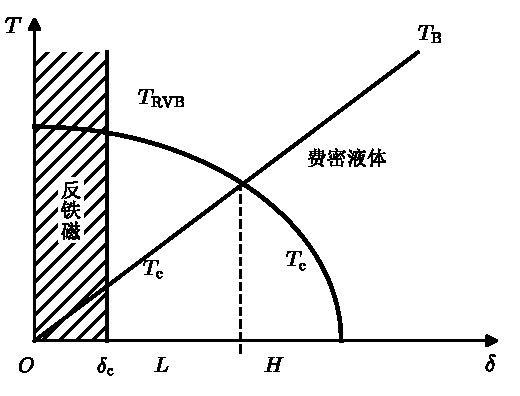
\includegraphics[width=6.5cm]{fig11-20.pdf}\\{\small 图 11.20\quad 推广 t-J模型的示意相图(其中：L——欠掺杂区，H——过掺杂区)}
\end{minipage}
\end{center}

已形成了d波配对，并存在自旋能隙，此即实验上在欠掺杂区所观测到的正常态能隙.这个具有d波对称性的能隙，在发生空穴子的玻色凝聚后，将变成超导能隙，并且有相同的 $\mathrm{d}_{x^{2}-y^{2}}$ 对称性.此外，在过掺杂区，当 $T_{\mathrm{B}}>T>T_{\mathrm{RVB}}$ 时，由于系统尚未进入共振价键状态，载流子仍然是既带电荷又有自旋的费密子，属于费密液体.福山等人还将t-J模型推广为可计入第二近邻跃迁 $t'$ 和第三近邻跃迁 $t''$ 的一个实用模型，用于计算掺杂La-214 与Y-123 等不同结构的高温超导体特性，包括计算这些化合物的非弹性中子衍射和核磁共振特性等，并且也取得了与实验测量定性一致的良好结果.有兴趣的读者可查阅文献\textsuperscript{[35]}中所列出的相关文献.

尽管基于安德逊共振价键态的超导理论能够说明大多数高温超导态与正常态特征，但是共振价键理论的基本假定(电荷与自旋分离)在两维情况下尚无严格的理论支持.仅仅在一维强关联系统中，根据赫伯德模型的严格解，理论研究已证明\textsuperscript{[36]}，低能激发可以用自旋与电荷分离的形式描写，此即一维拉亭格液体的特征.正因如此，当前强关联电子系统的一个理论研究热点是发展二维拉亭格液体理论.

在本节结束时，我们还将指出：在理论表述中描述角动量具有d波对称性时常采用 $(\cos k_{x}-\cos k_{y})$，而在实验研究中则习惯于用 $(\hat{k}_{x}^{2}-\hat{k}_{y}^{2})=\cos 2\phi$，其中 $\phi=\arctan(\hat{k}_{y}/\hat{k}_{x})$，$\hat{k}_{x}$ 与 $\hat{k}_{y}$ 是k空间单位矢 $\hat{\boldsymbol{k}}\ (|\hat{\boldsymbol{k}}|=1)$ 沿 x 与 y 方向的分量.其实只需对 $\cos k_{\alpha}\ (\alpha=x,y)$ 作形式上的级数展开，立刻可以看出 $(\cos k_{x}-\cos k_{y})$ 展开式的每一项均含有共同因子 $(k_{x}^{2}-k_{y}^{2})$，它是随k取向的快变函数，剩下的只是取向的缓变函数.再将k归一化为 $\hat{\boldsymbol{k}}$，可得到 $(\cos k_{x}-\cos k_{y})$ 正比于 $(\hat{k}_{x}^{2}-\hat{k}_{y}^{2})=\cos 2\phi$.换句话说，超导态的能隙和正常态的能隙都具有 $\mathrm{d}_{x^{2}-y^{2}}$ 对称性，与实验观测结果一致.

\section{巡游电子的磁性理论}

在第三章中我们已经证明，对于绝缘磁性材料产生磁性的局域电子在各原子周围形成局域自旋矩，它们之间的交换作用由海森伯模型描述.但是，在过渡金属中产生磁性的d电子不是局域电子，它们依次在各原子的 d轨道上游移，布洛赫称之为巡游电子(itinerant electron)，实际上就是公有化的能带电子.显然，对于巡游电子海森伯模型不成立，人们必须考虑能带电子的关联效应，从赫伯德模型入手建立巡游电子的磁性理论.根据式(11.1.13)，有外磁场 h 时的赫伯德哈密顿量为
\begin{equation}
\begin{aligned}
  &H=\sum_{k,\sigma}E_{k\sigma}n_{k\sigma}+U\sum_{l}n_{l\uparrow}n_{l\downarrow}\\
  &E_{k\sigma}=E_{k}+\sigma\mu_{\mathrm{B}}h\\
  &n_{k\sigma}=C_{k\sigma}^{+}C_{k\sigma},\quad n_{l\sigma}=C_{l\sigma}^{+}C_{l\sigma}
\end{aligned}
\end{equation}
我们将证明赫伯德哈密顿量的平均场近似(或哈特利-福克近似)就是斯通纳(Stoner)的能带磁性模型.若作无规相近似，则求得金属中的自旋波激发.

\subsection*{1. 斯通纳理论}

对H中的库仑项作哈特利-福克近似
\begin{equation}
  n_{l\uparrow}n_{l\downarrow}\approx\langle n_{l\uparrow}\rangle n_{l\downarrow}
  +\langle n_{l\downarrow}\rangle n_{l\uparrow}-\langle n_{l\uparrow}\rangle\langle n_{l\downarrow}\rangle
\end{equation}
略去等式右边的常数项并代入(11.11.1)，求得哈特利-福克近似的赫伯德哈密顿量
\begin{equation}
  H\approx\sum_{k,\sigma}E_{k\sigma}C_{k\sigma}^{+}C_{k\sigma}
  +U\sum_{l,\sigma}\langle n_{l\overline{\sigma}}\rangle C_{l\sigma}^{+}C_{l\sigma}
\end{equation}
在均匀情况下 $\langle n_{l\overline{\sigma}}\rangle$ 应与格点位置无关，这时可设
\begin{equation}
  \langle n_{\overline{\sigma}}\rangle=\langle n_{l\overline{\sigma}}\rangle
\end{equation}
再利用表象变换关系
\begin{equation}
  \sum_{l}C_{l\sigma}^{+}C_{l\sigma}=\sum_{k}C_{k\sigma}^{+}C_{k\sigma}
\end{equation}
将式(11.11.3)写成对角形式
\begin{equation}
  H\approx\sum_{k,\sigma}\widetilde{E}_{k\sigma}C_{k\sigma}^{+}C_{k\sigma}
\end{equation}
其中
\begin{equation}
  \widetilde{E}_{k\sigma}=E_{k\sigma}+U\langle n_{\overline{\sigma}}\rangle
  =E_{k}+\sigma\mu_{\mathrm{B}}h+U\langle n_{\overline{\sigma}}\rangle
\end{equation}
代表巡游电子的能量.即使在外磁场 $h=0$ 时，由于 $U\langle n_{\overline{\sigma}}\rangle$ 项的存在，$\widetilde{E}_{k\sigma}$ 仍与自旋取向有关.这时能带按自旋取向分裂，导致能带分裂的原因是由于反平行自旋电子之间的库仑排斥作用.不难证明，$U\langle n_{\overline{\sigma}}\rangle$ 项将给出一个与磁化强度M成正比的分子场.

\subsection*{(i) 分子场}

令
\begin{equation}
\left.\begin{aligned}
  &n=\langle n_{\uparrow}\rangle+\langle n_{\downarrow}\rangle\\
  &m=\langle n_{\downarrow}\rangle-\langle n_{\uparrow}\rangle
\end{aligned}\right\}
\end{equation}
其中n为平均每个元胞中的巡游电子数，$\boldsymbol{m}$ 代表相对磁化.当元胞数为N、样品取单位体积时，磁化强度
\begin{equation}
  \boldsymbol{M}=N\boldsymbol{\mu}_{\mathrm{B}}\boldsymbol{m}
\end{equation}
利用式(11.11.8)，求得
\begin{equation}
  \langle n_{\sigma}\rangle=\frac{1}{2}(n-\sigma m)=\frac{1}{2}\biggl(n-\sigma\frac{M}{N\mu_{\mathrm{B}}}\biggr)
  \qquad(\sigma=\pm 1)
\end{equation}
因此，式(11.11.7)写为
\begin{equation}
  \widetilde{E}_{k\sigma}=\biggl(E_{k}+\frac{1}{2}nU\biggr)
  +\sigma\mu_{\mathrm{B}}\biggl(h+\frac{U}{2N\mu_{\mathrm{B}}^{2}}M\biggr)
\end{equation}
上式表明，对赫伯德模型作HF近似可求出一个与M成正比的分子场
\begin{equation}
  h_{M}=\frac{U}{2N\mu_{\mathrm{B}}^{2}}M
\end{equation}
这就是斯通纳能带模型的出发点.当 $\boldsymbol{h}=\boldsymbol{0}$ 时若求得 $\langle n_{\uparrow}\rangle\neq\langle n_{\downarrow}\rangle$，则系统具有自发磁化，代表铁磁相.这时巡游电子在同一格点上的库仑作用使能带按自旋取向分裂，产生自旋朝上与向下电子数的不平衡，从而形成铁磁相，如图11.21所示，其↑、↓自旋的能带劈裂为
\begin{equation*}
  (\widetilde{E}_{k\uparrow}-\widetilde{E}_{k\downarrow})
  =U(\langle n_{\downarrow}\rangle-\langle n_{\uparrow}\rangle)\equiv 2\Delta
\end{equation*}
这里 $\langle n_{\sigma}\rangle$ 应自洽决定，而 $\Delta=\mu_{\mathrm{B}}h_{M}$.

\begin{center}
\begin{minipage}{6cm}
\centering
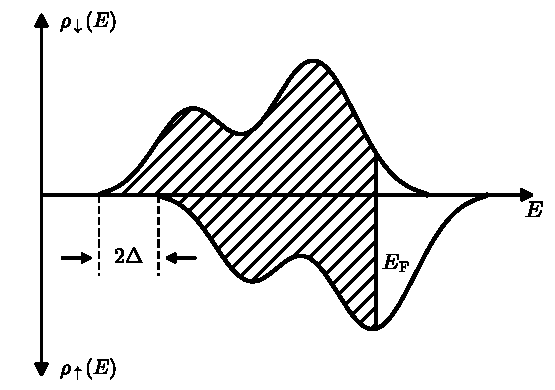
\includegraphics[width=6cm]{fig11-21.pdf}\\{\small 图 11.21\quad 过渡金属的 FM 相示意图\\
$\rho_{\uparrow}(E)$ 为自旋朝上的能带态密度，$\rho_{\downarrow}(E)$ 为自旋同下的能带态密度}
\end{minipage}
\end{center}

由于在哈特利-福克近似下哈密顿量已写成独立电子系统的标准对角化形式，根据式(11.11.6)，巡游电子在布洛赫态 $(\boldsymbol{k},\boldsymbol{\sigma})$ 上的占据数为
\begin{equation}
  \langle n_{k\sigma}\rangle=\langle C_{k\sigma}^{+}C_{k\sigma}\rangle=f(\widetilde{E}_{k\sigma})
\end{equation}
其中f是费密分布函数，适当选取能量的原点可消去式(11.11.11)中常数项 $\frac{1}{2}nU$，将 $\widetilde{E}_{k\sigma}$ 写成
\begin{equation}
\begin{aligned}
  \widetilde{E}_{k\sigma}&=E_{k}+\sigma\mu_{\mathrm{B}}\biggl(h+\frac{U}{2N\mu_{\mathrm{B}}^{2}}M\biggr)\\
  &=E_{k}+\sigma\mu_{\mathrm{B}}h+\sigma\Delta
\end{aligned}
\end{equation}
利用平移对称性，从式(11.11.4)可得
\begin{equation}
\begin{aligned}
  \langle n_{\sigma}\rangle&=\langle n_{l\sigma}\rangle=\frac{1}{N}\sum_{l}\langle n_{l\sigma}\rangle
  =\frac{1}{N}\sum_{k}\langle n_{k\sigma}\rangle\\
  &=\frac{1}{N}\sum_{k}f(\widetilde{E}_{k\sigma})
\end{aligned}
\end{equation}
代入式(11.11.9)，求得磁化强度为
\begin{equation}
\begin{aligned}
  M(T)&=N\mu_{\mathrm{B}}(\langle n_{\downarrow}\rangle-\langle n_{\uparrow}\rangle)\\
  &=\mu_{\mathrm{B}}\sum_{k}\{f(\widetilde{E}_{k\downarrow})-f(\widetilde{E}_{k\uparrow})\}
\end{aligned}
\end{equation}
当 $\boldsymbol{h}=\boldsymbol{0}$ 时，由上式可确定自发磁化与温度的关系.当 $h\neq 0$ 时，由此可以导出巡游电子系统形成铁磁相的条件.

\subsection*{(ii) 斯通纳判据}

讨论巡游电子系统中顺磁(PM)相的失稳条件，可以确定形成铁磁相的判据.设 $h=0$ 时系统处于顺磁相，有 $\langle n_{\uparrow}\rangle=\langle n_{\downarrow}\rangle$ 解.由于 $M\sim h$，当弱磁场 h作用时可以在式(11.11.16)中将 $f(\widetilde{E}_{k\sigma})$ 按h展开，求得
\begin{equation}
  M(T)\approx\mu_{\mathrm{B}}\biggl(2\mu_{\mathrm{B}}h+\frac{U}{N\mu_{\mathrm{B}}}M\biggr)
  \int_{0}^{\infty}\biggl[-\frac{\partial f(E)}{\partial E}\biggr]\rho(E)\mathrm{d}E
\end{equation}
其中 $\rho(E)$ 为能带的态密度.对于自由电子气体，取 $U=0$，得到
\begin{equation*}
  M(T)=\chi_{\mathrm{P}}(T)h
\end{equation*}
其中
\begin{equation}
  \chi_{\mathrm{P}}(T)=2\mu_{\mathrm{B}}^{2}\int_{0}^{\infty}
  \biggl(-\frac{\partial f}{\partial E}\biggr)\rho(E)\mathrm{d}E
\end{equation}
代表自由电子气体的泡利磁化率.当 $U\neq 0$ 时，对于巡游电子
\begin{equation}
  M(T)=\frac{\chi_{\mathrm{p}}(T)}{1-2\frac{U}{N}[\chi_{\mathrm{p}}(T)/4\mu_{\mathrm{B}}^{2}]}h
  \equiv\chi_{0}(T)h
\end{equation}
由此得到顺磁相的静态磁化率为
\begin{equation}
  \chi_{0}^{-1}(T)=\chi_{\mathrm{p}}^{-1}(T)-2\frac{U}{N}
\end{equation}
这里取 $4\mu_{\mathrm{B}}^{2}$ 为磁化率的单位.

当 $\chi_{0}^{-1}(T)<0$ 时顺磁相失稳，形成铁磁相.因此，根据式(11.11.20)，铁磁磁序的稳定条件为
\begin{equation}
  2\biggl(\frac{U}{N}\biggr)\chi_{\mathrm{p}}(T)>1
\end{equation}
当 $T=0$ K 时，由于 $-\dfrac{\partial f}{\partial E}=\delta(E-E_{\mathrm{F}})$，因此以 $4\mu_{\mathrm{B}}^{2}$ 为单位的泡利磁化率：
\begin{equation*}
\begin{aligned}
  \chi_{\mathrm{p}}(T=0)&=\frac{1}{2}\int\delta(E-E_{\mathrm{F}})\rho(E)\mathrm{d}E\\
  &=\frac{1}{2}\rho(E_{\mathrm{F}})
\end{aligned}
\end{equation*}
由式(11.11.21)，求得零温度时形成铁磁序的条件为
\begin{equation}
  (U/N)\rho(E_{\mathrm{F}})>1
\end{equation}
这就是铁磁相的斯通纳判据，铁磁相与顺磁相转变的相界由条件
\begin{equation}
  \chi_{0}^{-1}=0
\end{equation}
决定.例如从 $\chi_{0}^{-1}(T_{\mathrm{C}})=0$，可确定转变的居里温度 $T_{\mathrm{C}}$.

\subsection*{(iii) $T>T_{\mathrm{C}}$ 的磁化率}

对于铁磁金属，当 $T>T_{\mathrm{C}}$ 时实验上观察到磁化率满足居里-外斯（Curie-Weiss)定律
\begin{equation}
  \chi_{0}(T)=\frac{C}{T-T_{\mathrm{C}}}
\end{equation}
我们将证明斯通纳的巡游电子理论不能解释这个简单规律.根据式(11.11.20)，温度T时以 $4\mu_{\mathrm{B}}^{2}$ 为单位的磁化率为
\begin{equation}
  \chi_{0}(T)=\frac{\chi_{\mathrm{p}}(T)}{1-2I\chi_{\mathrm{p}}(T)}
\end{equation}
其中
\begin{equation*}
  I\equiv\frac{U}{N}
\end{equation*}
而泡利磁化率
\begin{equation*}
  \chi_{\mathrm{p}}(T)=\frac{1}{2}\int_{0}^{\infty}\biggl(-\frac{\partial f}{\partial E}\biggr)\rho(E)\mathrm{d}E
\end{equation*}
由于金属磁体的居里温度 $T_{\mathrm{c}}\sim 10^{2}\sim 10^{3}\ \mathrm{K}$，而费密温度 $T_{\mathrm{F}}=E_{\mathrm{F}}/k_{\mathrm{B}}\sim 10^{4}\sim 10^{5}\ \mathrm{K}$，$T_{\mathrm{F}}$ 高于金属熔点.因此，即使在 $T>T_{\mathrm{C}}$ 温区仍然有 $T\ll T_{\mathrm{F}}$ 关系，这时可算出上述费密积分
\begin{equation}
  \chi_{\mathrm{p}}(T)=\frac{1}{2}\rho_{\mathrm{F}}\biggl[1-\frac{\pi^{2}}{12}\biggl(\frac{T}{T_{\mathrm{F}}}\biggr)^{2}\biggr]
\end{equation}
它只是温度的缓变函数.代入式(11.11.25)，求得 $T>T_{\mathrm{C}}$ 时顺磁相的静态磁化率
\begin{equation}
  \chi_{0}(T)=\frac{\dfrac{1}{2}\rho_{\mathrm{F}}\biggl[1-\dfrac{\pi^{2}}{12}\biggl(\dfrac{T}{T_{\mathrm{F}}}\biggr)^{2}\biggr]}
  {[1-I\rho_{\mathrm{F}}]+I\rho_{\mathrm{F}}\dfrac{\pi^{2}}{12}\biggl(\dfrac{T}{T_{\mathrm{F}}}\biggr)^{2}}
\end{equation}
其中 $\rho_{\mathrm{F}}\equiv\rho(E_{\mathrm{F}})$ 代表费密面上的态密度.顺磁与铁磁相的转变温度 $\boldsymbol{T}_{\mathrm{C}}$ 由条件
\begin{equation}
  \chi_{0}^{-1}(T_{\mathrm{c}})=0
\end{equation}
决定.从式(11.11.28)可定出
\begin{equation}
  T_{\mathrm{C}}=T_{\mathrm{F}}\sqrt{\frac{12}{\pi^{2}}\biggl(\frac{I\rho_{\mathrm{F}}-1}{I\rho_{\mathrm{F}}}\biggr)}
\end{equation}
将此结果代入式(11.11.27)，经整理后得到磁化率与温度T的定性关系
\begin{equation}
  \chi_{0}(T)\sim\frac{T_{\mathrm{F}}^{2}}{T^{2}-T_{\mathrm{C}}^{2}}
\end{equation}
显然，这个结果与居里-外斯定律不同.因此，斯通纳的巡游电子理论不能说明 $T>T_{\mathrm{C}}$ 时磁化率的居里-外斯定律.这是理论应用于有限温区所遇到的一个重要困难.

\subsection*{(iv) 自发磁化}

令 $\widetilde{E}_{k\sigma}$ 中外磁场 $\boldsymbol{h}=\boldsymbol{0}$，从式(11.11.8)可得自发磁化方程为
\begin{equation}
\begin{aligned}
  m=\frac{M(T)}{N\mu_{\mathrm{B}}}&=\frac{1}{N}\sum_{k}(\langle n_{k\downarrow}\rangle-\langle n_{k\uparrow}\rangle)\\
  &=\frac{1}{N}\sum_{k}\{f(\widetilde{E}_{k\downarrow})-f(\widetilde{E}_{k\uparrow})\}\\
  &=\frac{1}{N}\sum_{k}\biggl\{\frac{1}{\mathrm{e}^{\beta(E_{k}-\Delta-\mu)}+1}
  -\frac{1}{\mathrm{e}^{\beta(E_{k}+\Delta-\mu)}+1}\biggr\}
\end{aligned}
\end{equation}
其中 $\beta=(k_{\mathrm{B}}T)^{-1}$，$\boldsymbol{\mu}$ 为化学势，而
\begin{equation*}
  \Delta\equiv\mu_{\mathrm{B}}h_{M}=\frac{1}{2}U(\langle n_{\downarrow}\rangle-\langle n_{\uparrow}\rangle)
\end{equation*}
$\boldsymbol{2\Delta}$ 代表↑与↓自旋能带的劈裂.当材料的能带态密度为已知时，原则上从式(11.11.31)可直接求出磁化强度与温度的关系.详细的计算见文献\textsuperscript{[37]}，在这里仅作定性介绍.从式(11.11.31)可知，磁化强度由↑、↓自旋带中电子数之差决定.因此其零温饱和磁化M(0)并不要求所有电子的自旋取向一致，这是斯通纳模型不同于海森伯模型的特点.例如当 $\mu\gg\Delta$ 时，从式(11.11.31)可求出
\begin{equation}
  \frac{M(0)}{N\mu_{\mathrm{B}}}\approx 2\Delta\int\biggl(-\frac{\partial f}{\partial E}\biggr)_{T=0}\rho(E)\mathrm{d}E
  =(2\Delta)\rho(E_{\mathrm{F}})
\end{equation}
这时平均每个元胞内的有效玻尔磁子数由能带劈裂和费密面上态密度之乘积决定，它是一个任意数，未必等于1.由此可知，在金属磁体中平均每个元胞内的零温饱和磁化强度不一定是玻尔磁子的整倍数，与实验结果一致.这是能带模型的成功之处.

当 $T\neq 0$ K 时，将产生从↓自旋带向↑自旋带的热激发.于是在↑自旋带中产生电子，而在↓自旋带中留下空穴.这种改变自旋的电子-空穴对激发称为斯通纳激发.随着温度升高斯通纳激发将使↑、↓自旋带的分裂减小，并造成 $M(T)$ 随T升高而下降，利用费密积分的索末菲展开式
\begin{equation*}
  \int_{0}^{\infty}\frac{\rho(E)}{\mathrm{e}^{\beta(E-\mu\pm\Delta)}+1}\mathrm{d}E
  =\int_{0}^{\mu\mp\Delta}\rho(E)\mathrm{d}E
  +\frac{\pi^{2}}{6}(k_{\mathrm{B}}T)^{2}\biggl(\frac{\mathrm{d}\rho}{\mathrm{d}E}\biggr)_{\mu\mp\Delta}+\cdots
\end{equation*}
从式(11.11.31)可求出在低温范围内
\begin{equation}
  \Delta M\equiv M(0)-M(T)\sim T^{2}
\end{equation}
此结果与实验测量的 $\Delta M\sim T^{3/2}$ 规律不符.这是因为斯通纳理论仍是独立电子模型，其中热激发的电子和空穴是分别独立地在平均场中运动的.在斯通纳理论中只考虑了自旋的个别激发，而忽略了自旋的集体激发.根据第三章的讨论，$\Delta M\sim T^{3/2}$ 是著名的布洛赫规律，它代表色散曲线为 $\omega=Dq^{2}$ 的自旋波激发所产生的磁化强度下降规律，这是自旋的集体激发效应.人们必须超出哈特利-福克近似，计及电子-空穴对的互作用，才能求得金属中的自旋波.我们将在“2”中用无规相近似法讨论这个问题.

\subsection*{(v) 斯通纳表述}

{\emergencystretch=2em
为了便于读者阅读有关金属磁性的文献，我们将介绍斯通纳关于铁磁性的表述.\allowbreak 根据公式(11.11.16)，以 $2\mu_{\mathrm{B}}$ 为单位的磁化强度
\begin{equation}
  M=\frac{1}{2}(N_{\downarrow}-N_{\uparrow})=\frac{1}{2}Nm
\end{equation}\par}
其中 $N_{\sigma}$ 代表自旋取向为 $\boldsymbol{\sigma}$ 的电子数，N为格点数，而m仍代表相对磁化，在这里 $N_{\sigma}=\langle n_{\sigma}\rangle N$.考虑到总电子数 $N_{e}=N_{\uparrow}+N_{\downarrow}$，平均每格点的电子浓度为 $\boldsymbol{n}=(N_{\mathrm{e}}/N)$.斯通纳引入下列量纲为1的磁序参量：
\begin{equation}
  \zeta\equiv(N_{\downarrow}-N_{\uparrow})/N_{\mathrm{e}}\qquad(0\leqslant\zeta\leqslant 1)
\end{equation}
对于铁磁相 $(\zeta\neq 0)$ 有关系式
\begin{equation}
  N_{\downarrow}=\frac{1}{2}N_{\mathrm{e}}(1+\zeta),\quad
  N_{\uparrow}=\frac{1}{2}N_{\mathrm{e}}(1-\zeta)
\end{equation}
说明↑与↓自旋的电子在k空间所占的相体积不同.对于球形等能面有 $k_{\sigma}^{\mathrm{max}}=(6\pi^{2}N_{\sigma})^{1/3}$，若再取顺磁相 $(\zeta=0)$ 的 $k_{\mathrm{F}}=(3\pi^{2}N_{e})^{1/3}$ 为波数的单位，构成的量纲为1的波数为 $k_{\sigma}\equiv(k_{\sigma}^{\mathrm{max}}/k_{\mathrm{F}})=(2N_{\sigma}/N_{\mathrm{e}})^{1/3}$，由此求得↑，↓电子的费密球半径为
\begin{equation}
  k_{\downarrow}=(1+\zeta)^{1/3},\quad k_{\uparrow}=(1-\zeta)^{1/3}
\end{equation}
当存在铁磁序 $(\zeta>0)$ 时，量纲为1的半径 $k_{\downarrow}>k_{\uparrow}$，如图11.22所示.

\begin{center}
\begin{minipage}{5.5cm}
\centering
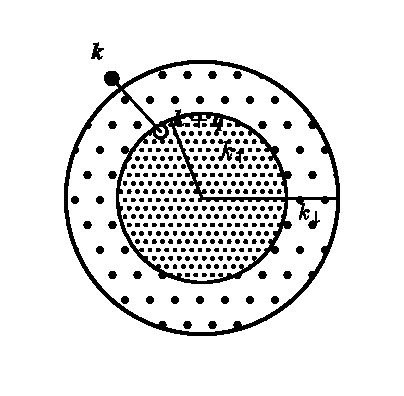
\includegraphics[width=5.5cm]{fig11-22.pdf}\\{\small 图 11.22\quad 铁磁相中↑、↓电子的费密球}
\end{minipage}
\end{center}

在无外磁场时，自旋↓与↑电子间的能带劈裂
\begin{equation}
\begin{aligned}
  2\Delta&=U(\langle n_{\downarrow}\rangle-\langle n_{\uparrow}\rangle)\\
  &=U(N_{\downarrow}-N_{\uparrow})/N\\
  &=Un\zeta
\end{aligned}
\end{equation}
利用式(11.11.14)并在球形等能面情况下取 $E_{k}=(k^{2}/2m_{\mathrm{e}}^{*})$，可将 $N_{\sigma}$ 表示为
\begin{equation*}
  N_{\sigma}=\sum_{k}f(E_{k\sigma})=\int_{0}^{\infty}\mathrm{d}E\,\rho(E)f(E+\sigma\Delta)
\end{equation*}
其中 $\rho(E)=(2m_{\mathrm{e}}^{*})^{3/2}\sqrt{E}/4\pi^{2}$，再利用索末菲展开式，即可求出 $\boldsymbol{T}=\boldsymbol{0}$ K时
\begin{equation*}
  N_{\sigma}=\frac{(2m_{\mathrm{e}}^{*})^{3/2}}{6\pi^{2}}(\mu-\sigma\Delta)^{3/2}
\end{equation*}
或更明确地写成下列表示式：
\begin{subequations}
\begin{equation}
  N_{\mathrm{e}}=\frac{N_{\mathrm{e}}}{2E_{\mathrm{F}}^{3/2}}\{(\mu+\Delta)^{3/2}+(\mu-\Delta)^{3/2}\}
\end{equation}
\begin{equation}
  2\Delta=\frac{nU}{2E_{\mathrm{F}}^{3/2}}\{(\mu+\Delta)^{3/2}-(\mu-\Delta)^{3/2}\}
\end{equation}
\end{subequations}
其中 $\boldsymbol{\mu}$ 为零温化学势，若再将 $\boldsymbol{\Delta}$ 与 $\boldsymbol{\mu}$ 均取 $E_{\mathrm{F}}$ 为能量的单位，则量纲为1的 $\boldsymbol{\mu}$ 和 $\varDelta$ 满足
\begin{subequations}
\begin{equation}
  1=\frac{1}{2}\{(\mu+\Delta)^{3/2}+(\mu-\Delta)^{3/2}\}
\end{equation}
\begin{equation}
  \zeta=\frac{1}{2}\{(\mu+\Delta)^{3/2}-(\mu-\Delta)^{3/2}\}
\end{equation}
\end{subequations}
最后求得
\begin{equation}
\begin{aligned}
  \genfrac{}{}{0pt}{}{\mu}{\Delta}\biggr\}&=\frac{1}{2}\bigl[(1+\zeta)^{2/3}\pm(1-\zeta)^{2/3}\bigr]\\
  &=\frac{1}{2}(k_{\downarrow}^{2}\pm k_{\uparrow}^{2})
\end{aligned}
\end{equation}
以上表示将对自旋波频谱的计算带来方便.若再将式(11.11.38)也写成量纲为1的表示式 $\Delta=(nU\zeta/2E_{\mathrm{F}})$，又可求得下列决定零温铁磁序参量 $\boldsymbol{\zeta}$ 的自洽方程：
\begin{equation}
\begin{aligned}
  (nU/2E_{\mathrm{F}})\zeta&=\frac{1}{2}\bigl[(1+\zeta)^{2/3}-(1-\zeta)^{2/3}\bigr]\\
  &\equiv R(\zeta)
\end{aligned}
\end{equation}
其中 $\boldsymbol{\zeta}$ 由等式左边的 $R=(nU/2E_{\mathrm{F}})\zeta$ 直线与等式右边的 $R(\zeta)$ 曲线之交点决定，如图11.23所示，由于 $R(\zeta)$ 曲线之斜率在 $\zeta=0$ 点与 $\zeta=1$ 点分别为 $(2/3)$ 与 $\infty$，可以求得3种不同的解：①顺磁解 $(\zeta=0)$：当 $(nU/2E_{\mathrm{F}})<2/3$ 时；②不完全的铁磁解 $(0<\zeta<1)$：当 $2^{-1/3}>(nU/2E_{\mathrm{F}})>2/3$ 时；③完全(饱和)铁磁解 $(\boldsymbol{\zeta}=1)$：当 $(nU/2E_{\mathrm{F}})>2^{-1/3}$ 时.换句话说，存在非零铁磁序参量 $(\zeta>0)$ 的条件为 $(nU/2E_{\mathrm{F}})>2/3$.再考虑到费密面上任一自旋取向的态密度 $\rho(E_{\mathrm{F}})=(3n/4E_{\mathrm{F}})N$，最后求得的形成铁磁序条件为
\begin{equation*}
  U(3n/4E_{\mathrm{F}})=(U/N)\rho(E_{\mathrm{F}})>1
\end{equation*}
与铁磁相的斯通纳判据式(11.11.22)一致.

\begin{center}
\begin{minipage}{5cm}
\centering
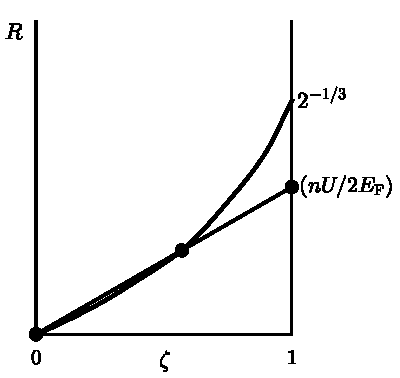
\includegraphics[width=5cm]{fig11-23.pdf}\\{\small 图 11.23\quad 确定磁序参量 $\zeta$ 的图示}
\end{minipage}
\end{center}

\subsection*{2. 金属中的自旋波}

如果超出哈特利-福克近似，用无规相近似方法讨论电子-空穴对的相互作用，可求出系统的集体激发——自旋波.在这里我们将用格林函数方法作无规相近似，其实质与第四章中讨论等离激元时所用运动方程线性化方法一致.

\subsection*{(i) 动态磁化率}

首先证明，以 $4\mu_{\mathrm{B}}^{2}$ 为单位的横向动态磁化率为
\begin{equation}
  \chi^{-+}(\boldsymbol{q},\omega)=-\langle\langle\hat{S}^{-}(\boldsymbol{q})|\hat{S}^{+}(-\boldsymbol{q})\rangle\rangle_{\omega+\mathrm{i}\eta}
\end{equation}
其中 $\hat{\boldsymbol{S}}^{\pm}(\boldsymbol{q},\omega)$ 代表自旋密度横向起伏的傅里叶分量，而格林函数 $\langle\langle\hat{S}^{-}(\boldsymbol{q})|\hat{S}^{+}(-\boldsymbol{q})\rangle\rangle_{\omega+\mathrm{i}\eta}$ 则描述金属中的自旋波.

设外磁场沿 $\nu$ 方向的分量为
\begin{equation}
  h_{\nu}(\boldsymbol{r},t)=h_{\nu}\mathrm{e}^{\mathrm{i}(\boldsymbol{q}\cdot\boldsymbol{r}-\omega t)}
\end{equation}
\begin{equation}
\begin{aligned}
  H_{\mathrm{e}}(t)&=-\sum_{\nu}\int\hat{M}_{\nu}(\boldsymbol{r})h_{\nu}\mathrm{e}^{\mathrm{i}\boldsymbol{q}\cdot\boldsymbol{r}}
  \mathrm{e}^{-\mathrm{i}(\omega+\mathrm{i}\eta)t}\mathrm{d}\boldsymbol{r}\\
  &=-\sum_{\nu}\hat{M}_{\nu}(-\boldsymbol{q})h_{\nu}\mathrm{e}^{-\mathrm{i}(\omega+\mathrm{i}\eta)t}\\
  &\equiv B\mathrm{e}^{-\mathrm{i}(\omega+\mathrm{i}\eta)t}
\end{aligned}
\end{equation}
其中 $\nu$ 方向磁化强度算符的傅里叶分量
\begin{equation}
  \hat{M}_{\nu}(\boldsymbol{q})=\int\hat{M}_{\nu}(\boldsymbol{r})\mathrm{e}^{-\mathrm{i}\boldsymbol{q}\cdot\boldsymbol{r}}\mathrm{d}\boldsymbol{r}
\end{equation}
而算符
\begin{equation}
  B=-\sum_{\nu}\hat{M}_{\nu}(-\boldsymbol{q})h_{\nu}
\end{equation}
根据久保公式
\begin{equation}
  \langle A(t)\rangle=\lim_{\eta\to+0}\mathrm{e}^{-\mathrm{i}(\omega+\mathrm{i}\eta)t}
  \langle\langle A|B\rangle\rangle_{\omega+\mathrm{i}\eta}
\end{equation}
取
\begin{equation}
  \boldsymbol{A}=\hat{\boldsymbol{M}}_{\nu}(\boldsymbol{q})
\end{equation}
可求得 $\mu$ 方向磁化强度的傅里叶分量为
\begin{equation}
\begin{aligned}
  \langle\hat{M}_{\mu}(\boldsymbol{q},\omega)\rangle&=-\sum_{\nu}
  \langle\langle\hat{M}_{\mu}(\boldsymbol{q})|\hat{M}_{\nu}(-\boldsymbol{q})\rangle\rangle_{\omega+\mathrm{i}\eta}h_{\nu}\\
  &\equiv\sum_{\nu}\chi_{\mu\nu}(\boldsymbol{q},\omega)h_{\nu}
\end{aligned}
\end{equation}
由于
\begin{equation}
  \hat{\boldsymbol{M}}=g\mu_{\mathrm{B}}\hat{\boldsymbol{S}}(\boldsymbol{r})
\end{equation}
其中 $S(\boldsymbol{r})$ 为自旋密度算符.因此，动态磁化率可以用自旋密度算符表示为
\begin{equation}
  \chi_{\mu\nu}(\boldsymbol{q},\omega)=-(g\mu_{\mathrm{B}})^{2}
  \langle\langle\hat{S}_{\mu}(\boldsymbol{q})|\hat{S}_{\nu}(-\boldsymbol{q})\rangle\rangle_{\omega+\mathrm{i}\eta}
\end{equation}
设电子的 $g=2$，并取 $4\mu_{\mathrm{B}}^{2}$ 为磁化率的单位，则求得横向动态磁化率为
\begin{equation}
  \chi^{-+}(\boldsymbol{q},\omega)=-\langle\langle\hat{S}^{-}(\boldsymbol{q})|\hat{S}^{+}(-\boldsymbol{q})\rangle\rangle_{\omega+\mathrm{i}\eta}
\end{equation}
其中 $\hat{\boldsymbol{S}}^{\pm}(\boldsymbol{q})$ 是自旋密度算符的傅里叶分量.根据附录中式(H.9)和(H.10)，$\hat{\boldsymbol{S}}^{\pm}(\boldsymbol{q})$ 可用电子算符表示成
\begin{equation}
\left.\begin{aligned}
  \hat{S}^{-}(\boldsymbol{q})&=\sum_{k}C_{k+q\downarrow}^{+}C_{k\uparrow}\\
  \hat{S}^{+}(-\boldsymbol{q})&=\sum_{k}C_{k-q\uparrow}^{+}C_{k\downarrow}
\end{aligned}\right\}
\end{equation}

\subsection*{(ii) 格林函数的无规相近似解}

从严格的赫伯德哈密顿量出发
\begin{equation*}
  H=\sum_{k,\sigma}E_{k}C_{k\sigma}^{+}C_{k\sigma}+U\sum_{l}n_{l\uparrow}n_{l\downarrow}
\end{equation*}
首先对上式作表象变换
\begin{equation*}
  C_{l\sigma}=\frac{1}{\sqrt{N}}\sum_{k}\mathrm{e}^{\mathrm{i}\boldsymbol{k}\cdot\boldsymbol{l}}C_{k\sigma}
\end{equation*}
写出布洛赫表象中的赫伯德哈密顿量
\begin{equation}
  H=H_{0}+H_{1}
\end{equation}
其中
\begin{equation}
  H_{0}=\sum_{k,\sigma}E_{k}C_{k\sigma}^{+}C_{k\sigma}
\end{equation}
\begin{equation}
  H_{1}=\frac{U}{N}\sum_{k,k',q}C_{k+q\uparrow}^{+}C_{k'-q\downarrow}^{+}C_{k'\downarrow}C_{k\uparrow}
\end{equation}
然后，利用格林函数运动方程求解.在格林函数的通式
\begin{equation}
  \omega\langle\langle A|B\rangle\rangle_{\omega}
  =\langle[A,B]\rangle-\langle\langle[H,A]|B\rangle\rangle_{\omega}
\end{equation}
中取
\begin{equation}
  B=\hat{S}^{+}(-\boldsymbol{q})=\sum_{k}C_{k-q\uparrow}^{+}C_{k\downarrow}
\end{equation}
\begin{equation}
  A=C_{k+q\downarrow}^{+}C_{k\uparrow}
\end{equation}
容易算出下列对易式
\begin{equation}
\begin{aligned}
  \langle[A,B]\rangle&=\sum_{k'}\langle[C_{k+q\downarrow}^{+}C_{k\uparrow},C_{k'-q\uparrow}^{+}C_{k'\downarrow}]\rangle\\
  &=\langle n_{k+q\downarrow}\rangle-\langle n_{k\uparrow}\rangle
\end{aligned}
\end{equation}
\begin{equation}
\begin{aligned}
  {}[H_{0},A]&=\sum_{k\sigma}E_{k}[C_{k\sigma}^{+}C_{k\sigma},C_{k+q\downarrow}^{+}C_{k\uparrow}]\\
  &=(E_{k+q}-E_{k})C_{k+q\downarrow}^{+}C_{k\uparrow}\\
  &=\omega_{kq}C_{k+q\downarrow}^{+}C_{k\uparrow}
\end{aligned}
\end{equation}
其中 $\omega_{kq}\equiv E_{k+q}-E_{k}$，库仑排斥项的对易式为
\begin{equation}
\begin{aligned}
  {}[H_{1},A]&=-\frac{U}{N}\sum_{k',q'}\bigl\{C_{k'+q'\uparrow}^{+}C_{k+q-q'\downarrow}^{+}C_{k'\uparrow}C_{k\uparrow}\\
  &\quad+C_{k+q\downarrow}^{+}C_{k'-q'\downarrow}^{+}C_{k'\downarrow}C_{k-q'\downarrow}\bigr\}
\end{aligned}
\end{equation}
由于上式右边含算符的四次项，代入格林函数方程的通式(11.11.58)将得到更高阶的格林函数.为了使格林函数方程封闭，我们将对式(11.11.63)的右边作平均场近似
\begin{equation}
\begin{aligned}
  {}[H_{1},A]&\approx U(\langle n_{\uparrow}\rangle-\langle n_{\downarrow}\rangle)C_{k+q\downarrow}^{+}C_{k\uparrow}\\
  &\quad+\frac{U}{N}(\langle n_{k+q\downarrow}\rangle-\langle n_{k\uparrow}\rangle)\sum_{k'}C_{k'+q\downarrow}^{+}C_{k'\uparrow}
\end{aligned}
\end{equation}
其中
\begin{equation*}
  \langle n_{\sigma}\rangle=\frac{1}{N}\sum_{k}\ \langle n_{k\sigma}\rangle
\end{equation*}
代入式(11.11.58)，得到线性化方程
\begin{equation}
\begin{aligned}
  &(\omega+\omega_{kq}-Um)\langle\langle C_{k+q\downarrow}^{+}C_{k\uparrow}|\hat{S}^{+}(-\boldsymbol{q})\rangle\rangle_{\omega}\\
  &=(\langle n_{k+q\downarrow}\rangle-\langle n_{k\uparrow}\rangle)
  \biggl\{1-\frac{U}{N}\sum_{k'}\langle\langle C_{k'+q\downarrow}^{+}C_{k'\uparrow}|\hat{S}^{+}(-\boldsymbol{q})\rangle\rangle_{\omega}\biggr\}\\
  &=(\langle n_{k+q\downarrow}\rangle-\langle n_{k\uparrow}\rangle)
  \biggl\{1-\frac{U}{N}\langle\langle\hat{S}^{-}(\boldsymbol{q})|\hat{S}^{+}(-\boldsymbol{q})\rangle\rangle_{\omega}\biggr\}
\end{aligned}
\end{equation}
其中
\begin{equation*}
  m=\langle n_{\downarrow}\rangle-\langle n_{\uparrow}\rangle
\end{equation*}
由此求得近似解
\begin{equation}
\begin{aligned}
  &\langle\langle C_{k+q\downarrow}^{+}C_{k\uparrow}|\hat{S}^{+}(-\boldsymbol{q})\rangle\rangle_{\omega}
  =\frac{f(E_{k+q\downarrow})-f(E_{k\uparrow})}{\omega+\omega_{kq}-Um}\times\\
  &\quad\biggl\{1-\frac{U}{N}\langle\langle\hat{S}^{-}(\boldsymbol{q})|\hat{S}^{+}(-\boldsymbol{q})\rangle\rangle_{\omega}\biggr\}
\end{aligned}
\end{equation}
这里取哈特利-福克近似的
\begin{equation}
\begin{aligned}
  &\langle n_{k\sigma}\rangle=f(E_{k\sigma})\\
  &E_{k\sigma}=E_{k}+U\langle n_{\overline{\sigma}}\rangle
\end{aligned}
\end{equation}
$\boldsymbol{f}$ 为费密分布函数，这种运动方程的线性化近似就是无规相近似，有时也称为动态平均场近似.根据式(11.11.54)，将式(11.11.66)对 k 求和后得到 $\langle\langle\hat{S}^{-}(\boldsymbol{q})|\hat{S}^{+}(-\boldsymbol{q})\rangle\rangle_{\omega}$.因此，铁磁相的无规相近似动态磁化率为
\begin{equation}
  \chi^{-+}(\boldsymbol{q},\omega)=-\langle\langle\hat{S}^{-}(\boldsymbol{q})|\hat{S}^{+}(-\boldsymbol{q})\rangle\rangle_{\omega+\mathrm{i}\eta}
  =\frac{\Gamma^{-+}(\boldsymbol{q},\omega)}{1-\dfrac{U}{N}\Gamma^{-+}(\boldsymbol{q},\omega)}
\end{equation}
其中
\begin{equation}
\begin{aligned}
  \Gamma^{-+}(\boldsymbol{q},\omega)&=-\sum_{k}\frac{f(E_{k+q\downarrow})-f(E_{k\uparrow})}
  {\omega+(E_{k+q\downarrow}-E_{k\uparrow})+\mathrm{i}\eta}\\
  &=\sum_{k}\frac{f(E_{k+q\uparrow})-f(E_{k\downarrow})}
  {\omega-(E_{k+q\uparrow}-E_{k\downarrow})+\mathrm{i}\eta}
\end{aligned}
\end{equation}
在后一等式中，作了变量代换 $\boldsymbol{k}\to-\boldsymbol{k}-\boldsymbol{q}\ (-\boldsymbol{k}\to\boldsymbol{k}+\boldsymbol{q})$ 并利用了 $\boldsymbol{E}_{-\boldsymbol{k}}=\boldsymbol{E}_{\boldsymbol{k}}$ 对称性.这时 $\Gamma^{-+}(\boldsymbol{q},\omega)$ 的极点为
\begin{equation}
  E_{k+q\uparrow}-E_{k\downarrow}=\omega_{kq}+Um
  =(E_{k+q}-E_{k})+U(\langle n_{\downarrow}\rangle-\langle n_{\uparrow}\rangle)
\end{equation}
对于顺磁相，$\langle n_{\uparrow}\rangle=\langle n_{\downarrow}\rangle$，$(E_{k+q\uparrow}-E_{k\downarrow})=(E_{k+q}-E_{k})$，这时
\begin{equation}
  \mathrm{Re}\,\Gamma^{-+}(q=0,\omega=0)=\sum_{k}\biggl(-\frac{\partial f}{\partial E_{k}}\biggr)=2\chi_{\mathrm{p}}(T)
\end{equation}
在这里 $\chi_{\mathrm{p}}(T)$ 就是自由电子气的泡利顺磁磁化率.由此可知，对于顺磁相，$\Gamma^{-+}(\boldsymbol{q},\omega)$ 代表无相互作用系统的横向动态磁化率.

\subsection*{(iii) 元激发谱}

互作用系统的元激发由格林函数 $\langle\langle\hat{S}^{-}|\hat{S}^{+}\rangle\rangle_{\omega}$（或 $\chi^{-+}$）的极点决定.根据式(11.11.68)，决定这些极点的本征方程为
\begin{equation}
  F(\omega)\equiv\frac{U}{N}\sum_{k}\frac{f(E_{k+q\uparrow})-f(E_{k\downarrow})}
  {\omega-(E_{k+q\uparrow}-E_{k\downarrow})}=1
\end{equation}
与等离激元问题相似，在 $\boldsymbol{T}=\boldsymbol{0}$ K 时作 $F(\omega)$ 曲线，它与直线 $F(\omega)=1$ 之交点代表系统的元激发.如图11.24所示.其中有一组准连续的交点落在 $F(\omega)$ 的发散点附近，可近似取为
\begin{equation}
  \omega=E_{k+q\uparrow}-E_{k\downarrow}=(E_{k+q}-E_{k})+U(\langle n_{\downarrow}\rangle-\langle n_{\uparrow}\rangle)
\end{equation}
此即 $\Gamma^{-+}(\boldsymbol{q},\omega)$ 的极点，它代表↑、↓自旋带之间的电子-空穴对激发，称为斯通纳激发或个别激发.当 $T=0$ K 时由于费密球的限制，斯通纳激发有上界 $\omega_{\mathrm{max}}$ 和下界 $\omega_{\mathrm{min}}$.从式(11.11.69)不难看出，在斯通纳区 $\omega_{\mathrm{min}}<\omega<\omega_{\mathrm{max}}$ 内 $\mathrm{Im}\,\Gamma^{-+}(\boldsymbol{q},\omega)\neq 0$，而在此区域之外 $\mathrm{Im}\,\Gamma^{-+}(\boldsymbol{q},\omega)=0$.这说明↑、↓自旋带之间的电子-空穴对个别激发(斯通纳激发)是有阻尼的.此外，在图11.24的低频端还存在一个交点，由于此交点落在斯通纳区之外 $(\omega<\omega_{\mathrm{min}})$，在零温时这个解是无阻尼的，它代表互作用系统的自旋集体振荡，即金属中的自旋波的色散曲线，可以讨论方程式(11.11.72)在长波和低频范围内的近似解.首先，对式(11.11.72)作变量代换，得到

\begin{center}
\begin{minipage}{7cm}
\centering
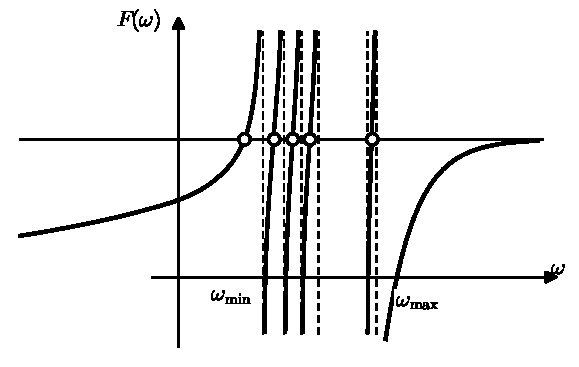
\includegraphics[width=7cm]{fig11-24.pdf}\\{\small 图 11.24\quad 方程式(11.11.72)的根}
\end{minipage}
\end{center}

\begin{equation}
  1=F(\omega)=\frac{U}{N}\sum_{k}\biggl\{\frac{f_{k\downarrow}}{mU-\omega+(E_{k+q}-E_{k})}
  -\frac{f_{k\uparrow}}{mU-\omega-(E_{k-q}-E_{k})}\biggr\}
\end{equation}
其中
\begin{equation}
  f_{k\sigma}\equiv f(E_{k\sigma})
\end{equation}
在长波范围内可作下列展开：
\begin{equation}
  E_{k\pm q}-E_{k}=\pm(\boldsymbol{q},\nabla)E_{k}+\frac{1}{2}(\boldsymbol{q}\cdot\nabla)^{2}E_{k}
\end{equation}
由于在铁磁相 $mU$ 取有限值，因此当 $q\to 0,\ \omega\to 0$ 时可取 $\omega/mU$ 和 $(E_{k\pm q}-E_{k})/mU$ 作为展开的小参量.将式(11.11.74)中分母展开到 $q^{2}$ 项，得到
\begin{equation*}
\begin{aligned}
  1=F(\omega)&=\biggl(1+\frac{\omega}{mU}\biggr)\frac{1}{mN}\sum_{k}(f_{k\downarrow}-f_{k\uparrow})
  -\frac{1}{2m^{2}UN}\sum_{k}(f_{k\uparrow}+f_{k\downarrow})(\boldsymbol{q}\cdot\nabla)^{2}E_{k}\\
  &\quad+\frac{1}{2m^{3}U^{2}N}\sum_{k}(f_{k\downarrow}-f_{k\uparrow})(\boldsymbol{q}\cdot\nabla E_{k})^{2}
\end{aligned}
\end{equation*}
考虑到
\begin{equation*}
  m=\langle n_{\downarrow}\rangle-\langle n_{\uparrow}\rangle=\frac{1}{N}\sum_{k}(f_{k\downarrow}-f_{k\uparrow})
\end{equation*}
并设 $E_{k}$ 为球形等能面.这时将有近似式
\begin{equation}
\begin{aligned}
  1=F(\omega)&=\biggl(1+\frac{\omega}{mU}\biggr)-\frac{q^{2}}{2m^{2}UN}\sum_{k}(f_{k\uparrow}+f_{k\downarrow})\nabla^{2}E_{k}\\
  &\quad+\frac{q^{2}}{3m^{2}U^{2}N}\sum_{k}(f_{k\downarrow}-f_{k\uparrow})(\nabla E_{k})^{2}
\end{aligned}
\end{equation}
由此求得自旋波的色散曲线
\begin{equation}
  \omega=Dq^{2}
\end{equation}
其中
\begin{equation}
  D=\frac{1}{2mN}\biggl\{\sum_{k}(f_{k\uparrow}+f_{k\downarrow})\nabla^{2}E_{k}
  -\frac{2}{3mU}\sum_{k}(f_{k\downarrow}-f_{k\uparrow})(\nabla E_{k})^{2}\biggr\}
\end{equation}
称为自旋波的劲度系数.我们将举例证明在球形等能面情况下 $\boldsymbol{D}>\boldsymbol{0}$.

例如 $\boldsymbol{T}=\boldsymbol{0}$ K时自旋波劲度系数D的计算.

在球形等能面情况，设 $E_{k}=(k^{2}/2m_{\mathrm{e}}^{*})$，这时 $\nabla^{2}E_{k}=(1/m_{\mathrm{e}}^{*})$，而 $(\nabla E_{k})^{2}=\nabla E_{k}\cdot\nabla E_{k}=(k/m_{\mathrm{e}}^{*})^{2}$，式(11.11.79)在取 $k_{\mathrm{F}}$ 为波数的单位时可改写为
\begin{equation*}
  D=\frac{1}{2m}\cdot\frac{k_{\mathrm{F}}^{2}}{2m_{\mathrm{e}}^{*}}\cdot\frac{1}{N}\sum_{k}(f_{k\uparrow}+f_{k\downarrow})
  -\frac{1}{3m^{2}NU}\cdot\frac{k_{\mathrm{F}}^{5}}{(m_{\mathrm{e}}^{*})^{2}}\sum_{k}(f_{k\downarrow}-f_{k\uparrow})k^{2}
\end{equation*}
其中相对磁化 $m=n\zeta$，而 $\boldsymbol{n}=(N_{\mathrm{e}}/N)$.当 $\boldsymbol{T}=\boldsymbol{0}$ K 时，考虑到
\begin{equation*}
  \frac{1}{N}\sum_{k}(f_{k\uparrow}+f_{k\downarrow})=N_{\mathrm{e}}/N=n
\end{equation*}
\begin{equation*}
\begin{aligned}
  \frac{1}{N}\sum_{k}(f_{k\downarrow}-f_{k\uparrow})k^{2}
  &=\frac{1}{2\pi^{2}}\biggl\{\int_{0}^{k_{\downarrow}}k^{4}\mathrm{d}k-\int_{0}^{k_{\uparrow}}k^{4}\mathrm{d}k\biggr\}\\
  &=\frac{1}{10\pi^{2}}(k_{\downarrow}^{5}-k_{\uparrow}^{5})
\end{aligned}
\end{equation*}
可将D写成
\begin{equation*}
  D=\frac{E_{\mathrm{F}}}{\zeta}\biggl\{1-\biggl(\frac{2E_{\mathrm{F}}}{mU}\biggr)\cdot\frac{1}{5}\cdot(k_{\downarrow}^{5}-k_{\uparrow}^{5})/\zeta\biggr\}
\end{equation*}
其中利用了 $k_{\mathrm{F}}^{3}=3\pi^{2}N_{\mathrm{e}}$ 和 $E_{\mathrm{F}}=(k_{\mathrm{F}}^{2}/2m_{\mathrm{e}}^{*})$.从式(11.11.38)可知 $\frac{1}{2}nU\zeta=\Delta$，再利用式(11.11.41)求得 $(nU\zeta/2E_{\mathrm{F}})=(k_{\downarrow}^{2}-k_{\uparrow}^{2})/2$.因此，在取 $\boldsymbol{E}_{\mathrm{F}}$ 为能量的单位时，所求出的自旋波劲度系数D为
\begin{equation*}
\begin{aligned}
  D&=\frac{1}{\zeta}\biggl\{1-\frac{2}{5}\frac{(k_{\downarrow}^{5}-k_{\uparrow}^{5})}{(k_{\downarrow}^{2}-k_{\uparrow}^{2})}\biggr\}\\
  &=\frac{1}{\zeta}\biggl\{1-\frac{2}{5}\frac{(1+\zeta)^{5/3}-(1-\zeta)^{5/3}}{(1+\zeta)^{2/3}-(1-\zeta)^{2/3}}\biggr\}>0
  \quad(0<\zeta\leqslant 1\ \text{时})
\end{aligned}
\end{equation*}
这就是 $\boldsymbol{D}>\boldsymbol{0}$ 的证明.显然，当 $\zeta\ll 1$ 时，经展开可得 $D\approx\zeta/9>0$，而当 $\boldsymbol{\zeta}\to 1$ 时(完全铁磁情形)，$D=1/5>0$.图 11.25 中绘出了自旋波的色散曲线，和斯通纳电子-空穴对激发区，其中集体激发位于个别激发区之下.显然，在低温区自旋波激发将起主要作用.利用自旋波色散关系 $\omega\sim q^{2}$，容易证明：由于激发自旋波量子所引起低温磁化的降低 $\Delta M\sim T^{3/2}$，与实验结果一致，改进了斯通纳(哈特利-福克近似)理论.

\begin{center}
\begin{minipage}{7cm}
\centering
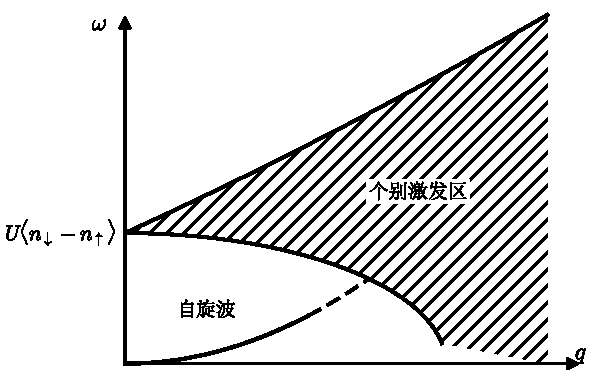
\includegraphics[width=7cm]{fig11-25.pdf}\\{\small 图 11.25\quad 铁磁金属的元激发谱}
\end{minipage}
\end{center}

\subsection*{3. HFA 和 RPA 理论的困难}

前面已经说明，从哈特利-福克近似理论不能推导出 $T>T_{\mathrm{C}}$ 时磁化率的居里-外斯定律，这是斯通纳理论应用于有限温度的主要困难.试问从无规相近似理论是否能得到居里-外斯定律？为此，我们讨论无规相近似的横向动态磁化率的长波 $(\boldsymbol{q}=0)$ 静态 $(\omega=0)$ 极限.根据式(11.11.68)—(11.11.71)，当 $T>T_{\mathrm{C}}$ 时顺磁相的长波静态磁化率为
\begin{equation}
  \chi^{-+}=\frac{\Gamma^{-+}(0,0)}{1-I\Gamma^{-+}(0,0)}
  =2\frac{\chi_{\mathrm{p}}(T)}{1-2I\chi_{\mathrm{p}}(T)}\qquad(q=0,\omega=0)
\end{equation}
其中 $I=U/N$.对于各向同性磁体，横向静态磁化率应为纵向之二倍.因此，从式(11.11.80)所求得的纵向静态顺磁磁化率
\begin{equation*}
  \chi_{0}(T)=\frac{\chi_{\mathrm{p}}(T)}{1-2I\chi_{\mathrm{p}}(T)}
\end{equation*}
它与哈特利-福克近似的磁化率公式(11.11.25)一样.在这里哈特利-福克近似和无规相近似理论碰到了相同的困难：$\chi_{0}(T)$ 的温度关系完全由泡利磁化率 $\chi_{\mathrm{p}}(T)$ 决定，而后者在 $T\ll T_{\mathrm{F}}$ 时只是温度的缓慢变化函数，它们都不能解释 $\boldsymbol{T}>\boldsymbol{T}_{\mathrm{C}}$ 时铁磁金属中所观察到的磁化率的居里-外斯定律.此外，从 $\chi_{0}^{-1}(T_{\mathrm{c}})=0$ 所求得居里温度 $T_{\mathrm{C}}$ 的理论值也比实测值高很多.

斯通纳理论在有限温度失败的原因是由于所采用的哈特利-福克近似对热激发效应估计不充分.它用↑，↓自旋带间电子与空穴的个别激发来说明金属磁的有限温度特性，认为电子和空穴是分别、独立的在平均场中运动，忽略了热激发的准粒子之间的关联作用.因此，斯通纳理论只是一种建立在单电子近似基础上的平均场理论，它所建立的热平衡图像是：$T=0$ K 时产生铁磁磁序的↑、↓自旋带分裂，将因温度升高和电子-空穴对激发加骤而逐渐减小.在 $T_{\mathrm{C}}$ 以上，就成为没有能带分裂的顺磁相，而具有泡利顺磁性.这就是斯通纳的热平衡态.从多体理论的角度，这样的描述是不完善的.实际上，在互作用系统中，热激发的电子和空穴之间的关联作用十分重要.首先，它将在铁磁金属中产生电子自旋密度的涨落，并以集体激发的形式传播，表现为各种 $\boldsymbol{q}$ 模式的自旋涨落波.当 $T<T_{\mathrm{C}}$ 时，相对于铁磁基态的自旋涨落可以近似用自旋波图像描述.其次，这些自旋涨落模还将通过模-模耦合作用对铁磁金属的热平衡态($\boldsymbol{q}=\boldsymbol{0}$模)产生重要的影响.无规相近似理论近似计算了相对于斯通纳热平衡态的自旋涨落，求得了金属中的自旋波激发等正确结果.但是，另一方面由于无规相近似略去了不同自旋模式之间的相互作用.因此，从无规相近似理论所求得的顺磁相磁化率仍然与斯通纳理论一样，也不能说明居里-外斯定律.在这个意义上人们常说无规相近似没有自洽的计入自旋涨落效应.现已明白，在铁磁金属中真正的顺磁态，不是斯通纳理论所描述的泡利顺磁性状态，它还应当包括各种可能激发的自旋涨落模，并且这些自旋涨落模式通过模-模耦合作用还将对斯通纳平衡态产生重要修正.因此，为了克服 $T>0$ K 时斯通纳理论的缺点，必须超出无规相近似范围，建立自洽计入自旋涨落效应的理论.在这方面日本物理学家守谷亨(Moriya)作出了重要贡献.他建立了弱铁磁金属自旋涨落的自洽重正化理论(self consistent renormalization theory，简称 SCR理论)\textsuperscript{[38]}，并在巡游电子模型中导出了磁化率的居里-外斯定律，其理论与弱铁磁金属如 $\mathrm{ZrZn_{2}}\,[T_{\mathrm{C}}=25\,\mathrm{K},\ M(0)/N\mu_{\mathrm{B}}=0.12]$ 和 $\mathrm{Sc_{3}In}\,[T_{\mathrm{C}}=6\,\mathrm{K},\ M(0)/N\mu_{\mathrm{B}}=0.04]$ 中的实验测量结果符合良好.SCR理论指出：在弱铁磁金属中由于长波自旋涨落压制磁化，将使 $T>T_{\mathrm{C}}$ 时静态磁化率服从居里-外斯定律，这是居里-外斯定律的新解释.

在20世纪80年代 SCR理论曾有较大的进展，并已超出弱铁磁金属范围成为巡游电子的自旋涨落理论.守谷亨曾寄希望于能够在自旋涨落理论的基础上建立金属磁性的统一图像\textsuperscript{[39]}.近年来自旋涨落的 SCR理论用于解释铜氧化合物高温超导体的正常态能隙也取得了成功\textsuperscript{[40]}.

\begin{canKao}
\begin{enumerate}[label={[\arabic*]}, leftmargin=2.2em, itemsep=0pt]
\item Hubbard J. Proc Roy Soc (London), 1963, A276: 238
\item Zubarev D N. Soviet Phys Usp (English Trasl), 1960, 3: 320
\item Hubbard J. Proc Roy Soc (London), 1964, A281: 401
\item Anderson P W. Phys Rev, 1961, 124: 41
\item Appelbaum J A. Lectures in Theoret Phys, 1971, XII-A: 41
\item Blandin A. J Appl Phys, 1967, 38: 1143
\item Leder H J, Mühlshlegel B. Z Phys, 1978, B29: 341
\item Kasuya T. Prog Theoret Phys (Kyoto), 1956, 16: 45
\item Ruberman M A, Kittle C. Phys Rev, 1954, 96: 99
\item Yosida K. Phys Rev, 1969, 106: 893
\item Nagamiya T. Solid State Physics, 1967, 20: 306
\item Darby M I. Am J Phys, 1969, 37: 354
\item Kittle C. Quantum Theory of Solids. New York: John Wiley and Sons Inc, 1963. Chap 18
\item Merzbacher E. Quantum Mechanics (2nd ed). New York: John Wiley and Sons Inc, 1970. Chap 12
\item van Vleck J H. Rev Mod Phys, 1962, 34: 681
\item Hathaway K B. Ultrathin Magnetic Structures. In: Heinrich B et al, ed. Berlin: Spinger--Verley, 1994. Chap 2
\item 李正中. 物理，1982，11：101
\item Kondo J. Solid State Physics, 1969, 23: 183
\item Yosida K. Phys Rev, 1966, 147: 223
\item Wilson K G. Rev Mod Phys, 1975, 47: 773
\item Andrei N. Phys Rev Lett, 1980, 45: 379
\item Wiegmann P B. Pis'ma Zh Eksep Teor Fiz, 1980, 31: 392
\item Schrieffer J R, Wolff P A. Phys Rev, 1966, 149: 491
\item Hewson A C. The Kondo Problem to Heavy Fermions. New York: Cambridge Univ Press, 1993
\item Degiorgi L. Rev Mod Phys, 1999, 71: 687
\item Coleman P S. Phys Rev, 1984, B29: 3035; 1987, B35: 5072
\item Read N, Newsn D M. Solid State Commun, 1984, 52: 993
\item Newsn D M, Read N. Adv Phys, 1987, 36: 799
\item Balacandran A P et al. Int J Mod Phys, 1990, 4: 2057
\item Zaanen J et al. Phys Rev, 1988, B37: 9423
\item Zhang F C, Rice T M. Phys Rev, 1988, B37: 3759; 1990, 41: 7243
\item Romberg H et al. Phys Rev, 1990, B42: 8768
\item Baskaram G, Zou Z, Anderson P W. Solid State Commun, 1987, 63: 973
\item Kotliar G, Liu J. Phys Rev, 1988, B38; 5142
\item Fukuyama H et al. Physica, 1997, 282--287: 124
\item Lieb E H, Wu F Y. Phys Rev Lett, 1968, 20: 1445
\item Wohlfarth E P. Rev Mod Phys, 1953, 25: 211
\item Moriya T. JMMM, 1979, 14: 1
\item Moriya T. Spin Fluctuations in Itinerant Electron Magmetisin. Berlin: Springer--Verlag, 1985
\item Imada M et al. Rev Mod Phys, 1998, 70: 1039
\end{enumerate}
\end{canKao}
% ============================================================
%  第十二章 无序系统（§1–§8 + 章末参考文献）
%  底本：高等教育出版社《固体理论》第二版；原书印刷页 486–532
%  （PDF 页 = 印刷页 + 20）
%  公式编号自检：§1 (12.1.1)–(12.1.16)（(12.1.2a/b/c) 为原书自带
%    二级编号，用 subequations 环境照录，与 ch06/ch07 体例一致）；
%    §2 (12.2.1)–(12.2.35)；§3 (12.3.1)–(12.3.29)；
%    §4 (12.4.1)–(12.4.26)；§5 (12.5.1)–(12.5.41)；
%    §6 (12.6.1)–(12.6.19)；§7 (12.7.1)–(12.7.30)
%    （(12.7.13a–d) 为原书自带二级编号，subequations 照录）；
%    §8 (12.8.1)–(12.8.22)。全章自动编号 223 个，无缺号
%    （任务单 tags=217 系 (12.2.24) tag 残作"(2.2.24)"、(12.2.35)
%    残作"(.35)"、(12.3.18)(12.7.21) 编号嵌于式内、(12.3.25)
%    (12.3.26) 编号被图 12.2 挤出为游离正文、(12.6.14) OCR 丢号
%    未计入所致）。
%
%  任务单所列"缺号"逐条对照原书页面判定（均非原书跳号）：
%    (12.2.24) OCR tag 残作"(2.2.24)"，原书 p493 在号；
%    (12.2.35) OCR tag 残作"(.35)"，原书 p494 在号（三行块，
%              编号在末行右端）；
%    (12.3.18) 编号嵌于式内（p497），已归还本式；
%    (12.3.25)(12.3.26) 原书 p498 此二式与图 12.2 左右并排，
%              编号被 OCR 挤成游离正文，已归位（先式后图）；
%    (12.6.14) OCR 丢号留式，原书 p515 在号（三行块末行编号）；
%    (12.7.21) 编号嵌于式内（p521），已归还本式。
%
%  已修正的 OCR/原书错误（除全角句点转"."、删 ~ 间隔符、收紧
%  \mathrm{d}、拆开行内公式与中文等常规项外）：
%  1. 原书 p495 (12.3.3) 印作 Ĥ=K̂(ω)+[H−K(ω)]^{-1}，指数 −1 为
%     原书排印衍文（本式为哈密顿量划分，下文明言"(H−K̂)取为
%     扰动项"，且 (12.3.4) 由此式直接导出），已删。
%  2. 原书 p508 (12.5.23) 第二行末因子印作 G_{l''l'}(E)，按代入
%     (12.5.21) 于 (12.5.22) 的推导应为 G_{l''l}(E)（与同系列
%     (12.5.25) 末因子 V_{l''l} 一致），已更正。
%  3. §1 "相距任意正格矢的两个原子"按 p486 补回"$l$"；
%     "可取 V_i=2Z IJIS 及近邻 W_ij=(−2 IJIS)"按 p488 复原为
%     V_i=2Z|J|S、W_ij=(−2|J|S)；"费密算子C与C代替"按 p488 复原
%     为"费密算子 C_i 与 C_i^+ 代替"。
%  4. (12.1.9) 整块 OCR 乱码按 p489 复原为
%     Σ_l{(ω−V_i)δ_il−W_il}G(l,j;ω)=δ_ij (i,j=1,…,N)；
%     (12.1.7) 后对易式按原书补回 a_j^+（[a_i,a_j^+]_±=δ_ij）。
%  5. §2.1 "散射效应却是可以严格计算的"OCR"可 j^μ 格计算"按
%     p490 复原；"直至 V̂ 的无穷阶"按原书补回 $\hat V$（p490）。
%  6. (12.2.4)(12.2.12)(12.2.16)(12.2.17)(12.2.24)(12.2.25)
%     (12.2.35) 等多行块 OCR 乱码按 p490–494 复原；求和条件
%     j(j≠i)、l(l≠j,≠i) 等照原书。
%  7. §3 (12.3.18) 整块 OCR 乱码按 p497 复原；(12.3.25)(12.3.26)
%     游离编号归位（见上）。
%  8. §4 (12.4.2)(12.4.3) 中 OCR \hat\varepsilon_i 按原书统一为
%     ξ_i；(12.4.13) 三段等式（含 2×2 逆矩阵分子）按 p502 复原；
%     (12.4.18) OCR"F_f(ω)"按 p503 复原为 F_ff(ω)；"分别对应于
%     取 ξ_i=1 和 0"、"由此可写出有效介质的平均场哈密顿量"
%     等 OCR 错乱句按 p501–502 复原。
%  9. §5 (12.5.16)(12.5.19)(12.5.21)(12.5.23)(12.5.25) 求和哑标
%     按原书 l''(l''≠l)、l''(l''≠l,l') 复原（OCR 误作 l'）；
%     (12.5.23) 整块按 p508 复原；(12.5.38) 按 p510 复原。
% 10. 原书两处脚注 OCR 漏失，按页脚补录：p507 脚注①（无限大
%     样品的热力学极限）、p509 脚注①（自回避路径）。
% 11. §6 (12.6.14) 三行式补号（原书在号）；"这里 R̄ 存在一个特征
%     温度 T_0，它表示当 R̄=R_0 时的温度"OCR 错乱按 p516 复原；
%     W_0 OCR 误作 Ψ_0 处按 p514–515 统一为 W_0。
% 12. §7 (12.7.2) OCR 分数乱码按 p517 复原为 (πħ/e²)(R/T)；
%     (12.7.21) 三行角平均积分按 p521 复原（末两项相同故为零，
%     照原书）；(12.7.9) 后文 dp/dE=1/v 的 OCR 乱码按 p518–519
%     复原；"当 d=1 时即使 L→0 也将得到一维横截面 A_1=1"按
%     p518 复原。
% 13. §8 (12.8.1) OCR 丢指数，按 p525 补 [N(E_F)L^d]^{-1}；
%     (12.8.5) 第二行 ln(g(L)/g_d)=−2αL 按 p526 复原；
%     (12.8.16) 幂指数 ν 与因子 g(L_0)/g(L) 按 p529 复原；
%     (12.8.22) OCR"\gimel"按 p531 复原为 β(g)；OCR"两级限"
%     按 p526 改"两极限"。
% 14. 超宽行修复（改断行，未改文字）：§3.3"又因为(1/N)Tr(P̂)=ℱ(ω)=…"与 §4.4 矩形/赫伯德型态密度两句的长行内公式按可断行单位拆分；§6"对于d维(d=1,2,3)系统"括号转全角；上述两段及§4.4 末段以局部 {\sloppy} 组消除 Overfull。
% 15. 图 12.1 位置：原书图占 p507 上半页，正文句"此外，含有高
%     浓度位错的固体，取向无规的微晶系统都属拓扑无序类"被图
%     隔断，重排本按文意连排后置图。
% 16. 文献[4][5]中文条目 OCR 缺空格/粘连按 p531 复原；西文条目
%     [11]"Economon"、[14]"Abrahans""Ramakrisbnan"、[19] 年份
%     卷号、[23]"1995.25"、[28] 卷号 42 等原书如此，未改。
%  插图：图 12.1–12.9 共 9 幅均为占位图（figures/fig12-N.pdf）；
%    图 12.1 含子图说明 (a)(b)(c)、图 12.6 含 (a)(b)，图 12.3
%    原书无图注文字（仅"图 12.3"），均照原书。
%  遗留问题：
%  · (12.5.40) 洛仑兹型分布原书分子印作 ZV（归一化的洛仑兹分布
%    应为 Γ/π 型），OCR 与原书一致，照录未改；
%  · §2.4 类似地一句原书印"x⩽1 的高浓度区域"（语义应为 x≈1），
%    照录未改；
%  · §8.4 "半导工艺"疑为"半导体工艺"衍漏（p530），照录未改；
%  · §4.2 "E_f−μ=k_BT_L 为小量"之 T_L 沿用原书记号（p502）；
%  · 文献[28] 卷号 42 与文献[14] 相同，疑为 79 之误，照原书。
% ============================================================
\chapter{无序系统}

\section{无序模型}

\subsection*{1. 无序的分类}

无序是相对于有序定义的，在固体系统中无序是指相对于完整晶体中原子排列的高度有序状态的偏离.完整晶体的特点是原子排列具有严格的周期重复性，可以用点阵描述理想晶体的结构特征，在这里不仅每个原子周围原子的排列有一定的规律，而且相距任意正格矢 $\boldsymbol{l}$ 的两个原子其周围的环境相同，这就是严格的周期性，又称为固体结构的长程序.当系统的理想周期性被破坏时，就失去了长程序，成为无序系统.

固体物理学中的无序系统包括含杂质、缺陷的晶体，无序合金以及非晶态固体材料等.无序系统大致可分为两类：

（i）成分无序（compositional disorder）

例如由A、B两种原子组成的二元无序合金，每个原子处于一个确定的格点上，但究竟是A原子还是B原子处于某格点上则是随机的，这时晶格虽然存在，原子排列的周期性已被破坏，在晶体中的 $\boldsymbol{r}$ 点与 $\boldsymbol{r}+\boldsymbol{l}$ 点从结构上讲已不再是等效点，失去了长程有序，如图12.1(b).如果把不同取向的自旋看作为不同的“原子”，则磁无序系统也可归入这一类.成分无序又称替代式无序.

（ii）拓扑无序（topological disorder）

晶格已不存在，但原子排列并不像气体中原子那么杂乱无章，在一个原子间距范围内原子排列还保持一定的秩序（短程序）表现为配位数或原子间化学键的键长，键角等平均不变.最典型的例子是非晶态半导体的Ge和Si的结构，四面体键组成无规网格，完全失去了周期性，但键长和键与键之间夹角基本保持不变，近邻配位数则未必保持不变.当价键不饱和时可能出现悬挂键（dangling bonds），这时配位数就发生了变化，图12.1(c)代表同时形成了悬挂键的拓扑无序系统.此外，含有高浓度位错的固体，取向无规的微晶系统都属拓扑无序类.

\begin{center}
\begin{minipage}{9.5cm}
\centering
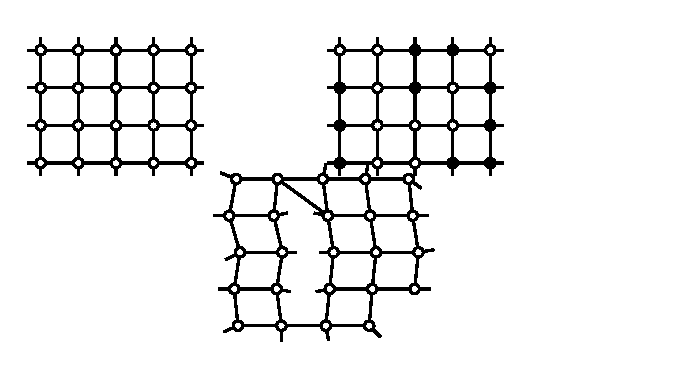
\includegraphics[width=9.5cm]{fig12-1.pdf}\\[0.3em]
{\small (a) 有序晶格\qquad\qquad (b) 成分无序系统}\\[0.2em]
{\small (c) 拓扑无序系统}\\[0.2em]
{\small 图 12.1}
\end{minipage}
\end{center}

\subsection*{2. 无序系统的模型哈密顿量}

米泽（Yonezawa）\textsuperscript{[1]}将描述固体中电子、声子和自旋波量子等各类独立准粒子系统的H用一个模型哈密顿量统一表示
\begin{equation}
  H=\sum_{i}V_{i}a_{i}^{+}a_{i}+\sum_{i\neq j}W_{ij}a_{i}^{+}a_{j}
\end{equation}
其中 $a_{i}^{+}$（$a_{i}$）是i格点上的准粒子产生（消灭）算符，$V_{i}$ 为准粒子在i格点的能量，$W_{ij}$ 描述准粒子在i与j格点之间转移的跃迁矩阵元.在此基础上，若将对角元 $V_{i}$ 取为无规变量，而 $W_{ij}$ 仍具有平移对称性，它只是 $(\boldsymbol{R}_{i}-\boldsymbol{R}_{j})$ 的函数，这时H属于对角无序系统.反之，若将 $V_{i}$ 当作与格点位置无关的常数，而取 $W_{ij}$ 与i和j格点位置以及格点上原子类型都有关的无规变量时，H将描述非对角无序系统.当 $V_{i}$ 与 $W_{ij}$ 都是无规变量时，将涉及既含对角无序，又有非对角无序的复杂无序系统.

选取式(12.1.1)统一表示H的理由来源于完整的有序晶格情形.因为当系统为有序时，H中的 $V_{i}$ 与 $W_{ij}$ 均具有平移对称性，表现为 $V_{i}=$ 常数和 $W_{ij}=W_{ij}\left(\boldsymbol{R}_{i}-\boldsymbol{R}_{j}\right)$.对于能带电子系统，当只考虑最近邻跃迁时可取 $V_{i}=\varepsilon\left(0\right)$ 及最近邻的 $W_{ij}=-J$，再将 $a_{i}$ 与 $a_{i}^{+}$ 用不计自旋标σ的费密算子 $C_{i}$ 与 $C_{i}^{+}$ 代替，上式立即简化为有序晶格中的紧束缚近似能量哈密顿量式(8.10.19).对于铁磁自旋波量子所组成的独立准粒子系统，$a_{i}$ 与 $a_{i}^{+}$ 应理解为描述自旋偏离的玻色算符，若再取 $V_{i}=2Z|J|S$ 及近邻 $W_{ij}=\left(-2|J|S\right)$，则描述有序铁磁系统的低激发态哈密顿量式(3.3.19)也可采用此模型哈密顿量.对于声子和夫伦克耳激子系统，情况也是相似的.因此，固体中各类独立元激发（准粒子）系统均可以概括为一个具有共同数学结构的模型哈密顿量，式(12.1.1).若在这一表示式的模型参数 $V_{i}$ 与 $W_{ij}$ 中引入表征无序的无规变量，H就成为描述无序系统（特别是成分无序系统）的统一哈密顿量.

我们首先讨论对角无序系统
\begin{subequations}
\begin{equation}
  H=H_{0}+H_{1}
\end{equation}
其中的有序项为
\begin{equation}
  H_{0}=\sum_{i\neq j}W_{ij}a_{i}^{+}a_{j}
\end{equation}
无序项则由
\begin{equation}
  H_{1}=\sum_{i}V_{i}a_{i}^{+}a_{i}
\end{equation}
\end{subequations}
表示，其中的 $V_{i}$ 是随机变化的.在二元无序合金 $\mathrm{A}_{x}\mathrm{B}_{1-x}$ 中，任一格点上可以被A或B原子占据的概率分别为x和(1−x)，因此i格点上 $V_{i}$ 的取值应根据概率分布
\begin{equation}
  P\left(V_{i}\right)=x\delta\left(V_{i}-V_{\mathrm{A}}\right)+\left(1-x\right)\delta\left(V_{i}-V_{\mathrm{B}}\right)
\end{equation}
决定，它既可能取 $V_{\mathrm{A}}$ 值，也可能取 $V_{\mathrm{B}}$，其中x为合金中A元素的浓度.有序项经傅里叶变换
\begin{equation*}
  W_{ij}=\frac{1}{N}\sum_{k}\varepsilon_{k}
  \mathrm{e}^{\mathrm{i}\boldsymbol{k}\cdot\left(\boldsymbol{R}_{i}-\boldsymbol{R}_{j}\right)}
\end{equation*}
可写成准粒子的能带项
\begin{equation}
  H_{0}=\sum_{k}\varepsilon_{k}a_{k}^{+}a_{k}
\end{equation}
其中 $\varepsilon_{k}$ 的能量原点取在能带的中央，相当于取 $W_{ii}=N^{-1}\sum_{k}\varepsilon_{k}=0$，这时 $W_{ij}$ 的逆变换可写为
\begin{equation}
  \varepsilon_{k}=\frac{1}{N}\sum_{i\neq j}W_{ij}
  \mathrm{e}^{-\mathrm{i}\boldsymbol{k}\cdot\left(\boldsymbol{R}_{i}-\boldsymbol{R}_{j}\right)}
\end{equation}

由于在无序系统中实际测得的物理量都是和各种无序微观相貌的平均有关的，因此对于无序系统的研究主要是计算其格林函数的无规平均
\begin{equation}
  \langle\hat{\boldsymbol{G}}\rangle=\prod_{i}\int\mathrm{d}V_{i}\,P\left(V_{i}\right)\hat{\boldsymbol{G}}
\end{equation}
为此，首先应当求出无序系统中格林函数矩阵 $\hat{\boldsymbol{G}}$ 所满足的方程.

\subsection*{3. 无序系统的格林函数方程}

定义格点格林函数
\begin{equation}
  G\left(i,j;\omega\right)\equiv\langle\langle a_{i}|a_{j}^{+}\rangle\rangle_{\omega}
\end{equation}
其中准粒子算符满足标准对易关系 $\left[a_{i},a_{j}^{+}\right]_{\pm}=\delta_{ij}$.再利用式(12.1.1)
\begin{equation}
  \left[a_{i},H\right]_{-}=V_{i}a_{i}+\sum_{l}W_{il}a_{l}
\end{equation}
并代入格林函数运动方程的通式(11.1.24)，求出格点格林函数在 $\omega$ 平面上的运动方程组
\begin{equation}
  \sum_{l}\left\{\left(\omega-V_{i}\right)\delta_{il}-W_{il}\right\}G\left(l,j;\omega\right)=\delta_{ij}
  \qquad\left(i,j=1,\cdots,N\right)
\end{equation}
这个方程组可以写成矩阵形式，定义下列（$N\times N$）矩阵
\begin{equation}
  \hat{\boldsymbol{W}}\equiv\left[W_{ij}\right],\qquad
  \hat{\boldsymbol{V}}\equiv\left[V_{i}\delta_{ij}\right],\qquad
  \hat{\boldsymbol{H}}=\hat{\boldsymbol{W}}+\hat{\boldsymbol{V}}
\end{equation}
其中 $\hat{\boldsymbol{V}}$ 为对角，而 $\hat{\boldsymbol{W}}$ 为非对角（因为取 $W_{ii}=0$）的（$N\times N$）矩阵.相应地定义格林函数矩阵
\begin{equation}
  \hat{\boldsymbol{G}}\equiv\left[G\left(i,j;\omega\right)\right]=\hat{\boldsymbol{G}}\left(\omega\right)
\end{equation}
这时可将格林函数运动方程组缩写为下列矩阵表示式：
\begin{equation}
  \left(\omega\hat{\boldsymbol{I}}-\hat{\boldsymbol{W}}-\hat{\boldsymbol{V}}\right)\hat{\boldsymbol{G}}=\hat{\boldsymbol{I}}
\end{equation}
其中 $\hat{\boldsymbol{I}}$ 代表（$N\times N$）的单位矩阵.因此，无序系统中准粒子格林函数的一般表示式为
\begin{equation}
  \hat{\boldsymbol{G}}\left(\omega\right)=\left(\omega\hat{\boldsymbol{I}}-\hat{\boldsymbol{H}}\right)^{-1}
\end{equation}
用于对角无序情形，取 $\hat{\boldsymbol{H}}_{0}=\hat{\boldsymbol{W}}$，可将 $\hat{\boldsymbol{H}}_{0}$ 的格林函数矩阵表示写成
\begin{equation}
  \hat{\boldsymbol{G}}_{0}\left(\omega\right)=\left(\omega\hat{\boldsymbol{I}}-\hat{\boldsymbol{W}}\right)^{-1}
  \ \text{或}\
  \left(\omega\hat{\boldsymbol{I}}-\hat{\boldsymbol{W}}\right)\hat{\boldsymbol{G}}_{0}=\hat{\boldsymbol{I}}
\end{equation}
从式(12.1.12)与式(12.1.14)可以导出
\begin{equation}
  \left(\omega\hat{\boldsymbol{I}}-\hat{\boldsymbol{W}}\right)
  \left(\hat{\boldsymbol{G}}-\hat{\boldsymbol{G}}_{0}\right)=\hat{\boldsymbol{V}}\hat{\boldsymbol{G}}
\end{equation}
由此求得对角无序系统中准粒子格林函数所满足的标准运动方程：
\begin{equation}
  \hat{\boldsymbol{G}}=\hat{\boldsymbol{G}}_{0}+\hat{\boldsymbol{G}}_{0}\hat{\boldsymbol{V}}\hat{\boldsymbol{G}}
\end{equation}
其中 $\hat{\boldsymbol{G}}_{0}$ 是有序系统 $\hat{\boldsymbol{H}}_{0}$ 的格林函数，它具有平移对称性.因此，在计算无序格林函数的无规平均 $\langle\hat{\boldsymbol{G}}\rangle$ 时，将涉及关联项 $\hat{\boldsymbol{V}}\hat{\boldsymbol{G}}$ 的无规平均 $\langle\hat{\boldsymbol{V}}\hat{\boldsymbol{G}}\rangle$.由于 $\hat{\boldsymbol{V}}\hat{\boldsymbol{G}}$ 可以用t矩阵表示，其无规平均 $\langle\hat{\boldsymbol{V}}\hat{\boldsymbol{G}}\rangle$ 的计算自然将涉及如何计算t矩阵的无序平均.

\section{\texorpdfstring{平均$ t $矩阵方法}{平均t矩阵方法}}

\subsection*{1. 无序系统的$ t $矩阵}

t矩阵定义为
\begin{equation}
  \hat{\boldsymbol{G}}=\hat{\boldsymbol{G}}_{0}+\hat{\boldsymbol{G}}_{0}\hat{T}\hat{\boldsymbol{G}}_{0}
\end{equation}
根据式(12.1.16)可求得 $\hat{\boldsymbol{G}}$ 的一个表示式
\begin{equation}
  \hat{\boldsymbol{G}}=\left(1-\hat{\boldsymbol{G}}_{0}\hat{\boldsymbol{V}}\right)^{-1}\hat{\boldsymbol{G}}_{0}
\end{equation}
再将上式代入式(12.1.16)求得
\begin{equation}
  \hat{\boldsymbol{G}}=\hat{\boldsymbol{G}}_{0}+\hat{\boldsymbol{G}}_{0}\hat{\boldsymbol{V}}
  \left(1-\hat{\boldsymbol{G}}_{0}\hat{\boldsymbol{V}}\right)^{-1}\hat{\boldsymbol{G}}_{0}
\end{equation}
因此无序系统的t矩阵可表示为
\begin{equation}
\begin{aligned}
  \hat{T}=\hat{T}\left(\omega\right)
  &=\hat{\boldsymbol{V}}\left(1-\hat{\boldsymbol{G}}_{0}\hat{\boldsymbol{V}}\right)^{-1}\\
  &=\hat{\boldsymbol{V}}+\hat{\boldsymbol{V}}\hat{\boldsymbol{G}}_{0}\hat{\boldsymbol{V}}
  +\hat{\boldsymbol{V}}\hat{\boldsymbol{G}}_{0}\hat{\boldsymbol{V}}\hat{\boldsymbol{G}}_{0}\hat{\boldsymbol{V}}+\cdots
\end{aligned}
\end{equation}
其中包括了对角无序 $\hat{\boldsymbol{V}}$ 所引起的相对于 $\hat{\boldsymbol{G}}_{0}$ 的所有散射，直至 $\hat{\boldsymbol{V}}$ 的无穷阶.

对 $\hat{\boldsymbol{G}}$ 取无规平均，可将式(12.2.1)表示为
\begin{equation}
  \langle\hat{\boldsymbol{G}}\rangle=\hat{\boldsymbol{G}}_{0}
  +\hat{\boldsymbol{G}}_{0}\langle\hat{T}\rangle\hat{\boldsymbol{G}}_{0}
\end{equation}
其中 $\hat{\boldsymbol{G}}_{0}$ 是有序系统的格林函数，无需平均.再定义自能
\begin{equation}
  \hat{\boldsymbol{\Sigma}}\left(\omega\right)\equiv
  \hat{\boldsymbol{G}}_{0}^{-1}-\langle\hat{\boldsymbol{G}}\rangle^{-1}
\end{equation}
又有
\begin{equation}
  \langle\hat{\boldsymbol{G}}\rangle=\hat{\boldsymbol{G}}_{0}
  +\hat{\boldsymbol{G}}_{0}\hat{\boldsymbol{\Sigma}}\left(\omega\right)\langle\hat{\boldsymbol{G}}\rangle
\end{equation}
利用式(12.2.5)—式(12.2.7)可求得自能 $\hat{\boldsymbol{\Sigma}}$ 与平均t矩阵 $\langle\hat{T}\rangle$ 的严格关系
\begin{equation}
  \hat{\boldsymbol{\Sigma}}=\left(1+\langle\hat{T}\rangle\hat{\boldsymbol{G}}_{0}\right)^{-1}\langle\hat{T}\rangle
\end{equation}
上式表明自能完全由 $\langle\hat{T}\rangle$ 决定.剩下的问题是如何计算 $\langle\hat{T}\rangle$？实际上 $\langle\hat{T}\rangle$ 不可能严格求出.但是，单个杂质相对于基体 $\hat{\boldsymbol{G}}_{0}$ 的散射效应却是可以严格计算的.为此，我们将先介绍单个原子的t矩阵.

\subsection*{2. 原子的$ t $矩阵}

为了严格计入在某一格点上单个无序杂质的多重散射效应，将 $\hat{\boldsymbol{V}}$ 分解为
\begin{equation}
  \hat{\boldsymbol{V}}\equiv\sum_{i}\hat{V}_{i}
\end{equation}
其中 $\hat{\boldsymbol{V}}$ 为（$N\times N$）对角矩阵.$\hat{V}_{i}$ 也是（$N\times N$）矩阵，但其中仅在i格点上有扰动 $V_{i}$，其它的对角元素 $(j\neq i)$ 均为零.再将式(12.2.4)改写成 $\hat{T}\left(1-\hat{\boldsymbol{G}}_{0}\hat{\boldsymbol{V}}\right)=\hat{\boldsymbol{V}}$，可得
\begin{equation}
  \hat{T}=\left(1+\hat{T}\hat{\boldsymbol{G}}_{0}\right)\hat{\boldsymbol{V}}
  =\sum_{i}\left[1+\Bigl(\sum_{j}\hat{T}_{j}\Bigr)\hat{\boldsymbol{G}}_{0}\right]\hat{V}_{i}
  =\sum_{i}\hat{T}_{i}
\end{equation}
其中 $\hat{T}_{i}$ 表示在含有多杂质的无序系统中i格点对 $\hat{T}$ 矩阵的贡献
\begin{equation}
  \hat{T}_{i}=\hat{V}_{i}+\Bigl(\sum_{j}\hat{T}_{j}\Bigr)\hat{\boldsymbol{G}}_{0}\hat{V}_{i}
  =\left(\hat{V}_{i}+\hat{T}_{i}\hat{\boldsymbol{G}}_{0}\hat{V}_{i}\right)
  +\sum_{j(j\neq i)}\hat{T}_{j}\hat{\boldsymbol{G}}_{0}\hat{V}_{i}
\end{equation}
上式中最后一项代表其它格点 $j\left(j\neq i\right)$ 的影响，而前两项则是同格点的贡献.若将来自i格点上单个原子的t矩阵定义为
\begin{equation}
\begin{aligned}
  \hat{t}_{i}&\equiv\hat{V}_{i}\left(1-\hat{\boldsymbol{G}}_{0}\hat{V}_{i}\right)^{-1}\\
  &=\hat{V}_{i}+\hat{V}_{i}\hat{\boldsymbol{G}}_{0}\hat{V}_{i}
  +\hat{V}_{i}\hat{\boldsymbol{G}}_{0}\hat{V}_{i}\hat{\boldsymbol{G}}_{0}\hat{V}_{i}+\cdots
\end{aligned}
\end{equation}
这是一个准至 $V_{i}$ 无穷阶的“部分求和”，它计入了单个原子的全部多重散射.因此，在物理上 $\hat{t}_{i}$ 描述一个波被第i个原子的完全散射，而在数学上 $\hat{t}_{i}$ 相当于略去式(12.2.11)等式右边最后一项（即略去来自 $j\neq i$ 的贡献）时所求出的近似 $\hat{T}_{i}$.至于严格的 $\hat{T}_{i}$ 应当从式(12.2.11)的下列等效表示式
\begin{equation}
  \hat{T}_{i}\left(1-\hat{\boldsymbol{G}}_{0}\hat{V}_{i}\right)
  =\hat{V}_{i}+\sum_{j(j\neq i)}\hat{T}_{j}\hat{\boldsymbol{G}}_{0}\hat{V}_{i}
\end{equation}
导出，由此求得 $\hat{T}_{i}$ 的严格公式
\begin{equation}
  \hat{T}_{i}=\hat{t}_{i}+\sum_{j(j\neq i)}\hat{T}_{j}\hat{\boldsymbol{G}}_{0}\hat{t}_{i}
\end{equation}
其中除来自i格点的贡献外，还包括了i格点以外的其它(N−1)个格点上的原子对i格点上波的散射效应.再作迭代运算，就求得整个无序系统的t矩阵
\begin{equation}
\begin{aligned}
  \hat{T}=\sum_{i}\hat{T}_{i}
  &=\sum_{i}\hat{t}_{i}+\sum_{i}\sum_{j(j\neq i)}\hat{t}_{j}\hat{\boldsymbol{G}}_{0}\hat{t}_{i}\\
  &\quad+\sum_{i}\sum_{j(j\neq i)}\sum_{l(l\neq j,\neq i)}
  \hat{t}_{l}\hat{\boldsymbol{G}}_{0}\hat{t}_{j}\hat{\boldsymbol{G}}_{0}\hat{t}_{i}+\cdots
\end{aligned}
\end{equation}
显然，当计算 $\langle\hat{T}\rangle$ 时将涉及不同格点上原子t矩阵的散射关联项，如 $\langle\hat{t}_{j}\hat{\boldsymbol{G}}_{0}\hat{t}_{i}\rangle$、$\langle\hat{t}_{l}\hat{\boldsymbol{G}}_{0}\hat{t}_{j}\hat{\boldsymbol{G}}_{0}\hat{t}_{i}\rangle$ 等无穷个关联项，在原则上是无法严格求解的.人们只能求助于各种近似，其中最常用的是平均t矩阵近似（简称ATA）的单格点近似（简称SSA）.

\subsection*{3. ATA 的单格点近似}

SSA略去了不同格点间散射的关联，仅对 $\hat{T}$ 中各格点的原子t矩阵（如 $\hat{t}_{i}$、$\hat{t}_{j}$ 和 $\hat{t}_{l}$）独立取无规平均，这时SSA的ATA表示式为
\begin{equation}
\begin{aligned}
  \langle\hat{T}\rangle&=\sum_{i}\langle\hat{t}_{i}\rangle
  +\sum_{j(j\neq i)}\langle\hat{t}_{j}\rangle\hat{\boldsymbol{G}}_{0}\sum_{i}\langle\hat{t}_{i}\rangle\\
  &\quad+\sum_{l(l\neq j)}\langle\hat{t}_{l}\rangle\hat{\boldsymbol{G}}_{0}\sum_{j(j\neq i)}\langle\hat{t}_{j}\rangle
  \hat{\boldsymbol{G}}_{0}\sum_{i}\langle\hat{t}_{i}\rangle+\cdots
\end{aligned}
\end{equation}
同时可将式(12.2.14)的无规平均写成下列SSA表示式
\begin{equation}
\begin{aligned}
  \langle\hat{T}_{i}\rangle&=\langle\hat{t}_{i}\rangle
  +\sum_{j(j\neq i)}\langle\hat{T}_{j}\rangle\hat{\boldsymbol{G}}_{0}\langle\hat{t}_{i}\rangle\\
  &=\left(1+\langle\hat{T}\rangle\hat{\boldsymbol{G}}_{0}\right)\langle\hat{t}_{i}\rangle
  -\langle\hat{T}_{i}\rangle\hat{\boldsymbol{G}}_{0}\langle\hat{t}_{i}\rangle
\end{aligned}
\end{equation}
经整理，求得单格点近似下无序系统的平均t矩阵
\begin{equation}
  \langle\hat{T}\rangle=\sum_{i}\langle\hat{T}_{i}\rangle
  =\left(1+\langle\hat{T}\rangle\hat{\boldsymbol{G}}_{0}\right)\sum_{i}\langle\hat{t}_{i}\rangle
  \left(1+\hat{\boldsymbol{G}}_{0}\langle\hat{t}_{i}\rangle\right)^{-1}
\end{equation}
将上式代入自能公式(12.2.8)，又可求出SSA的自能矩阵
\begin{equation}
  \hat{\boldsymbol{\Sigma}}_{\mathrm{SSA}}=\sum_{i}\langle\hat{t}_{i}\rangle
  \left(1+\hat{\boldsymbol{G}}_{0}\langle\hat{t}_{i}\rangle\right)^{-1}
\end{equation}
和相应的格林函数矩阵
\begin{equation}
  \langle\hat{\boldsymbol{G}}\rangle_{\mathrm{SSA}}
  =\left(\hat{\boldsymbol{G}}_{0}^{-1}-\hat{\boldsymbol{\Sigma}}_{\mathrm{SSA}}\right)^{-1}
\end{equation}

现在讨论二元无序合金 $\mathrm{A}_{x}\mathrm{B}_{1-x}$ 中A与B原子的t矩阵 $\hat{t}_{\mathrm{A}(\mathrm{B})}$ 的表示式.从原子t矩阵的定义式(12.2.12)可知，$\hat{t}_{i}$ 与 $\hat{V}_{i}$ 相似只有第i个对角元 $V_{i}$ 为非零.当i格点被A（或B）原子占据时，其对角矩阵元定义为
\begin{equation}
  t_{\mathrm{A}(\mathrm{B})}\equiv\langle i|\hat{t}_{\mathrm{A}(\mathrm{B})}|i\rangle
\end{equation}
根据二元无序合金的概率分布公式(12.1.3)可求出i格点上原子t矩阵的无规平均 $\langle\hat{t}_{i}\rangle$ 的唯一非零对角元为
\begin{equation}
  xt_{\mathrm{A}}+\left(1-x\right)t_{\mathrm{B}}
\end{equation}
显然它与i无关，因此 $\Bigl\langle\sum_{i}\hat{t}_{i}\Bigr\rangle$ 是对角矩阵，并且每个对角元均相同，可写成
\begin{equation}
  \Bigl\langle\sum_{i}\hat{t}_{i}\Bigr\rangle=x\hat{t}_{\mathrm{A}}+\left(1-x\right)\hat{t}_{\mathrm{B}}
\end{equation}
其中 $\Bigl\langle\sum_{i}\hat{t}_{i}\Bigr\rangle$、$\hat{t}_{\mathrm{A}}$ 和 $\hat{t}_{\mathrm{B}}$ 都是（$N\times N$）对角矩阵.为了求出 $t_{\mathrm{A}}$ 和 $t_{\mathrm{B}}$ 的表示式，应从（$N\times N$）无规矩阵 $\sum_{i}\hat{t}_{i}$ 入手，计算其第i个对角元
\begin{equation}
\begin{aligned}
  t_{i}&=\langle i|\hat{t}_{i}|i\rangle
  =\langle i|\left(\hat{V}_{i}+\hat{V}_{i}\hat{\boldsymbol{G}}_{0}\hat{V}_{i}
  +\hat{V}_{i}\hat{\boldsymbol{G}}_{0}\hat{V}_{i}\hat{\boldsymbol{G}}_{0}\hat{V}_{i}+\cdots\right)|i\rangle\\
  &=\frac{V_{i}}{1-\langle i|\hat{\boldsymbol{G}}_{0}|i\rangle V_{i}}
  =\frac{V_{i}}{1-\left(1/N\right)\left(\mathrm{Tr}\hat{\boldsymbol{G}}_{0}\right)V_{i}}
\end{aligned}
\end{equation}
其中利用了有序的格点格林函数的平移对称性，即利用了 $\langle i|\hat{\boldsymbol{G}}_{0}|i\rangle$ 与格点位置无关的特征：
\begin{equation}
\begin{aligned}
  \langle i|\hat{\boldsymbol{G}}_{0}|i\rangle
  &=\left(1/N\right)\sum_{i}\ \langle i|\hat{\boldsymbol{G}}_{0}|i\rangle\\
  &=\left(1/N\right)\mathrm{Tr}\hat{\boldsymbol{G}}_{0}\equiv F\left(\omega\right)
\end{aligned}
\end{equation}
$F\left(\omega\right)$ 称为未微扰的平均格点格林函数，也就是取 $H_{0}=\sum_{k}\varepsilon_{k}a_{k}^{+}a_{k}$ 时所求得的平均格林函数为 $F\left(\omega\right)=\left(1/N\right)\sum_{k}\left(\omega-\varepsilon_{k}\right)^{-1}$.

由于在 $\mathrm{A}_{x}\mathrm{B}_{1-x}$ 合金中无规变量 $V_{i}$ 只取 $V_{\mathrm{A}}$ 和 $V_{\mathrm{B}}$ 两个值，利用公式(12.2.24)可将A和B原子的散射矩阵元表示为
\begin{equation}
  t_{\mathrm{A}(\mathrm{B})}=\frac{V_{\mathrm{A}(\mathrm{B})}}{1-F\left(\omega\right)V_{\mathrm{A}(\mathrm{B})}}
\end{equation}
类似 $\Bigl\langle\sum_{i}\hat{t}_{i}\Bigr\rangle$ 矩阵，SSA的自能矩阵 $\hat{\boldsymbol{\Sigma}}_{\mathrm{SSA}}$ 也是对角的，并且N个对角元均相同，若将式(12.2.22)与(12.2.23)代入式(12.2.19)，可求得SSA自能的单位矩阵表示
\begin{equation}
  \hat{\boldsymbol{\Sigma}}_{\mathrm{SSA}}=\Sigma_{\mathrm{SSA}}\hat{\boldsymbol{I}}
\end{equation}
其中任一对角元均为
\begin{equation}
  \Sigma_{\mathrm{SSA}}=\frac{\left[xt_{\mathrm{A}}+\left(1-x\right)t_{\mathrm{B}}\right]}
  {1+F\left(\omega\right)\left[xt_{\mathrm{A}}+\left(1-x\right)t_{\mathrm{B}}\right]}
\end{equation}
以上是在单格点近似下ATA方法的基本框架.应用ATA方法，人们计算了二元无序合金的声子态密度，并求得了与实验定性一致的结果.但是ATA方法本身还存在欠缺和问题.

\subsection*{4. 存在的问题}

在作具体计算时，ATA方法存在的主要问题是：计算结果的好坏往往因有序参考晶体（又称基体）的不同选择而异，带有某种任意性.例如：

（i）分别取A或B原子构成基体，所得结果均不适用于全浓度区.对于B原子构成基体情形，可将未微扰项取为
\begin{equation}
  H_{0}=\sum_{k}\left(\varepsilon_{k}+V_{\mathrm{B}}\right)a_{k}^{+}a_{k}
\end{equation}
这时散射只发生在A原子上
\begin{equation*}
  t_{\mathrm{A}}=\frac{\left(V_{\mathrm{A}}-V_{\mathrm{B}}\right)}
  {1-F\left(\omega-V_{\mathrm{B}}\right)\left(V_{\mathrm{A}}-V_{\mathrm{B}}\right)},\qquad
  t_{\mathrm{B}}=0
\end{equation*}
其中有序的平均格林函数为
\begin{equation*}
  F\left(\omega-V_{\mathrm{B}}\right)\equiv\left(1/N\right)\sum_{k}
  \left[\left(\omega-V_{\mathrm{B}}\right)-\varepsilon_{k}\right]^{-1}
\end{equation*}
代入 $\Sigma_{\mathrm{SSA}}$ 公式后，经简单代数运算，求得自能的表示式
\begin{equation}
  \Sigma_{\mathrm{SSA}}^{\mathrm{B}}
  =\frac{x\left(V_{\mathrm{A}}-V_{\mathrm{B}}\right)}
  {1-\left(1-x\right)F\left(\omega-V_{\mathrm{B}}\right)\left(V_{\mathrm{A}}-V_{\mathrm{B}}\right)}
  \sim x
\end{equation}
类似的，当取A原子构成基体时，应设
\begin{equation}
  H_{0}=\sum_{k}\left(\varepsilon_{k}+V_{\mathrm{A}}\right)a_{k}^{+}a_{k}
\end{equation}
并且散射仅存在B原子上，
\begin{equation*}
  t_{\mathrm{A}}=0,\qquad
  t_{\mathrm{B}}=\frac{\left(V_{\mathrm{B}}-V_{\mathrm{A}}\right)}
  {1-F\left(\omega-V_{\mathrm{A}}\right)\left(V_{\mathrm{B}}-V_{\mathrm{A}}\right)}
\end{equation*}
最后求得
\begin{equation}
  \Sigma_{\mathrm{SSA}}^{\mathrm{A}}
  =\frac{\left(1-x\right)\left(V_{\mathrm{B}}-V_{\mathrm{A}}\right)}
  {1-xF\left(\omega-V_{\mathrm{A}}\right)\left(V_{\mathrm{B}}-V_{\mathrm{A}}\right)}
  \sim\left(1-x\right)
\end{equation}
当 $V_{\mathrm{A}}$ 和 $V_{\mathrm{B}}$ 间差别不大时，$\Sigma_{\mathrm{SSA}}^{\mathrm{B}}\sim x$ 仅适用于低浓度 $\left(x\ll1\right)$ 区，而不能推广到 $x\rightarrow1$ 的高浓度区，并且将与 $\Sigma_{\mathrm{SSA}}^{\mathrm{A}}\sim\left(1-x\right)$ 相抵触.类似地，$\Sigma_{\mathrm{SSA}}^{\mathrm{A}}\sim\left(1-x\right)$ 也只适用于 $x\leqslant1$ 的高浓度区域，它不能拓宽到 $x\ll1$ 区域.因此，这两种简单选取基体的方案都不能描述全浓度区 $\left(0<x<1\right)$ 中无序系统的特征.必须根据研究者的经验和直觉去猜测参考基体，以便求出 $\Sigma_{\mathrm{SSA}}\sim x\left(1-x\right)$ 的自能，才能用于全浓度区.

（ii）虚晶近似

当取
\begin{equation}
  \overline{V}\equiv\langle V_{i}\rangle=xV_{\mathrm{A}}+\left(1-x\right)V_{\mathrm{B}}
\end{equation}
为参考基体时，未微扰的有序基体设想为按照x(A)与(1−x)(B)混合的“虚拟原子”晶体，此即虚晶近似（virtual crystal approximation，VCA）.这时
\begin{equation}
  t_{\mathrm{A}(\mathrm{B})}
  =\frac{\left(V_{\mathrm{A}(\mathrm{B})}-\overline{V}\right)}
  {1-F\left(\omega-\overline{V}\right)\left(V_{\mathrm{A}(\mathrm{B})}-\overline{V}\right)}
\end{equation}
其中 $V_{\mathrm{A}}-\overline{V}=\left(1-x\right)\Delta$，$V_{\mathrm{B}}-\overline{V}=-x\Delta$，这里 $\Delta\equiv\left(V_{\mathrm{A}}-V_{\mathrm{B}}\right)$.因此
\begin{equation}
\begin{aligned}
  \langle\hat{t}_{i}\rangle&=xt_{\mathrm{A}}+\left(1-x\right)t_{\mathrm{B}}\\
  &=x\left(1-x\right)\left\{
  \frac{\Delta}{1-F\left(\omega-\overline{V}\right)\left(1-x\right)\Delta}
  -\frac{\Delta}{1+F\left(\omega-\overline{V}\right)x\Delta}\right\}\\
  &\approx x\left(1-x\right)F\left(\omega-\overline{V}\right)\Delta^{2}
\end{aligned}
\end{equation}
由此求出的虚晶近似自能函数也正比于 $x\left(1-x\right)$，适用于全浓度区 $\left(0<x<1\right)$.在复平面上的自能为
\begin{equation*}
  \Sigma^{\mathrm{VCA}}\left(\omega+\mathrm{i}\eta\right)
  \approx\left[x\left(1-x\right)\Delta^{2}\right]
  F\left(\omega+\mathrm{i}\eta-\overline{V}\right)
  \qquad\left(\eta=0^{+}\right)
\end{equation*}
考虑到 $F\left(\omega+\mathrm{i}\eta-\overline{V}\right)$ 的贡献主要来自虚部，并且对于电子系统近似等于 $-\mathrm{i}\pi\rho_{\mathrm{F}}$，其中 $\rho_{\mathrm{F}}$ 为费密面上的电子态密度.这时无序合金中电子自能的虚部为
\begin{equation*}
  \mathrm{Im}\,\Sigma^{\mathrm{VCA}}\left(\omega+\mathrm{i}\eta\right)
  \sim-x\left(1-x\right)\Delta^{2}
\end{equation*}
在固体物理学中，人们利用此结果定性地说明了合金电阻率随浓度x变化的规律，但虚晶近似只是一种低阶近似.

根据以上讨论可知，平均t矩阵近似法本身并未告诉人们如何选择良好的参考晶体，使计算结果难于控制.因此需要一种规范的自洽近似方法来选定参考晶体，使计算结果能有较大的改进，这就是人们提出相干势近似方法的背景.

\section{相干势近似}

由于平均t矩阵近似计算的结果完全取决于参考晶体的选择，如何保证选择良好是平均t矩阵近似法所未能解决的一个关键性问题，而相干势近似（CPA）则很好地解决了这个问题.

\subsection*{1. 相干势近似的主要思路}

相干势近似的主要思路首先由苏文（Soven）\textsuperscript{[2]}和泰勒（Taylor）\textsuperscript{[3]}提出.他们注意到，尽管无序系统的格林函数 $\hat{\boldsymbol{G}}=\left(\omega\hat{\boldsymbol{I}}-\hat{\boldsymbol{H}}\right)^{-1}$ 与哈密顿量 $\hat{\boldsymbol{H}}$ 均是无序的，但无规平均格林函数 $\langle\hat{\boldsymbol{G}}\rangle$，则是有序的.他们建议用某一有效介质（EM）的哈密顿量 $\hat{\boldsymbol{H}}_{\mathrm{eff}}\left(\omega\right)$ 来拟合无规平均格林函数
\begin{equation}
  \langle\hat{\boldsymbol{G}}\rangle=\left[\omega\hat{\boldsymbol{I}}-\hat{\boldsymbol{H}}_{\mathrm{eff}}\left(\omega\right)\right]^{-1}
\end{equation}
其中 $\hat{\boldsymbol{H}}_{\mathrm{eff}}\left(\omega\right)$ 应与 $\langle\hat{\boldsymbol{G}}\rangle$ 一样具有平移对称性（TS），也是一个有序量，而相干势近似的主要问题是：如何自洽地确定这一具有平移对称性的有效介质的哈密顿量 $\hat{\boldsymbol{H}}_{\mathrm{eff}}\left(\omega\right)$.

设某一良好近似的有效介质的哈密顿量为 $\hat{K}\left(\omega\right)$，由它构成的有效介质格林函数可写为
\begin{equation}
  \hat{\boldsymbol{P}}\left(\omega\right)=\left[\omega\hat{\boldsymbol{I}}-\hat{K}\left(\omega\right)\right]^{-1}
\end{equation}
这时若将无序系统的哈密顿量作如下划分
\begin{equation}
  \hat{\boldsymbol{H}}=\hat{K}\left(\omega\right)+\left[H-K\left(\omega\right)\right]
\end{equation}
并将 $\left(H-\hat{K}\right)$ 取为扰动项，则无序系统的格林函数可以用 $\left(\hat{\boldsymbol{H}}-\hat{K}\right)$ 扰动所产生的t矩阵 $\left(\hat{T}\right)$ 和有序的有效介质格林函数 $\left(\hat{\boldsymbol{P}}\right)$ 来表示
\begin{equation}
  \hat{\boldsymbol{G}}=\hat{\boldsymbol{P}}+\hat{\boldsymbol{P}}\hat{T}\hat{\boldsymbol{P}}
\end{equation}
取无规平均后应有
\begin{equation}
  \langle\hat{\boldsymbol{G}}\rangle=\hat{\boldsymbol{P}}+\hat{\boldsymbol{P}}\langle\hat{T}\rangle\hat{\boldsymbol{P}}
\end{equation}
显然，当无序系统相对于有效介质的平均散射 $\langle\hat{T}\rangle=0$ 时，必然有
\begin{equation}
  \langle\hat{\boldsymbol{G}}\rangle=\hat{\boldsymbol{P}}
\end{equation}
即无规平均格林函数正好等于 $\hat{\boldsymbol{P}}$.这时有效介质的哈密顿量已找出为
\begin{equation}
  \hat{\boldsymbol{H}}_{\mathrm{eff}}\left(\omega\right)=\hat{K}\left(\omega\right)
\end{equation}
至此相干势近似所提出的问题在原则上得到了解决.在这里确定 $\hat{\boldsymbol{H}}_{\mathrm{eff}}\left(\omega\right)$ 的关键是 $\hat{K}\left(\omega\right)$ 应满足下列条件：
\begin{equation}
  \langle\hat{T}\left[\hat{K}\left(\omega\right)\right]\rangle=0
\end{equation}
此即求解有效介质的严格自洽方程.根据前面的讨论可知，由于 $\langle\hat{T}\rangle$ 在原则上不可能严格求解，只有某种近似解（如SSA以及团簇近似等等）.人们只能做到近似求解自洽方程
\begin{equation}
  \langle\hat{T}_{\mathrm{approx}}\left[\hat{K}\left(\omega\right)\right]\rangle=0
\end{equation}
因此上式称为相干势近似的自洽方程.

当讨论对角无序情形时，可设有效介质的哈密顿量为
\begin{equation}
  K\left(\omega\right)=H_{0}+\sum_{i}u\left(\omega\right)a_{i}^{+}a_{i}
\end{equation}
其中待定的 $u\left(\omega\right)$ 称为相干势，而 $H_{0}=\sum_{i\neq j}W_{ij}a_{i}^{+}a_{j}=\sum_{k}\varepsilon_{k}a_{k}^{+}a_{k}$.这时，相干势近似归结为作数值计算以确定CPA自洽方程
\begin{equation}
  \langle T_{\mathrm{approx}}\left[u\left(\omega\right)\right]\rangle=0
\end{equation}
的相干势 $u\left(\omega\right)$，下面将讨论二元无序合金系统在单格点近似下的相干势近似问题.

\subsection*{2. 单格点近似的相干势近似自洽方程}

二元无序合金 $\mathrm{A}_{x}\mathrm{B}_{1-x}$ 的哈密顿量可以写成下列形式
\begin{equation}
  H=\sum_{i\neq j}W_{ij}a_{i}^{+}a_{j}+\sum_{i}E_{i}a_{i}^{+}a_{i}
\end{equation}
其中 $E_{i}$ 为二元合金（BRA）的无规势
\begin{equation}
  E_{i}=\xi_{i}E_{\mathrm{A}}+\left(1-\xi_{i}\right)E_{\mathrm{B}}
\end{equation}
其中 $E_{\mathrm{A}}$ 与 $E_{\mathrm{B}}$ 分别代表i格点被A或B原子占据时的准粒子能量，而 $\xi_{i}$ 则是无规变量，它定义为
\begin{equation}
  \xi_{i}=\begin{cases}1 & \left(i\in\mathrm{A}\right)\\ 0 & \left(i\in\mathrm{B}\right)\end{cases}
\end{equation}
其无规平均 $\langle\xi_{i}\rangle=x$ 代表A原子的浓度.

设有效介质的哈密顿量
\begin{equation}
  K\left(\omega\right)=\sum_{i\neq j}W_{ij}a_{i}^{+}a_{j}+\sum_{i}u\left(\omega\right)a_{i}^{+}a_{i}
\end{equation}
它是具有平移对称的有序量，无序系统相对有效介质的散射扰动势应取
\begin{equation}
  V_{i}=E_{i}-u\left(\omega\right),\qquad
  V_{\mathrm{A}(\mathrm{B})}=E_{\mathrm{A}(\mathrm{B})}-u\left(\omega\right)
\end{equation}
取无规平均后，得到
\begin{equation}
  \langle V_{i}\rangle=xV_{\mathrm{A}}+\left(1-x\right)V_{\mathrm{B}}
  =x\left(E_{\mathrm{A}}-u\right)+\left(1-x\right)\left(E_{\mathrm{B}}-u\right)
\end{equation}
类似本章§2中的讨论，相对于有效介质的散射t矩阵在单格点近似时为
\begin{equation}
\begin{aligned}
  \langle\hat{T}\rangle=\Bigl\{1&+\sum_{j(j\neq i)}\langle\hat{T}_{j}\rangle\hat{\boldsymbol{P}}
  +\sum_{l(l\neq j)}\langle\hat{T}_{l}\rangle\hat{\boldsymbol{P}}\sum_{j(j\neq i)}\langle\hat{t}_{j}\rangle\hat{\boldsymbol{P}}+\cdots\Bigr\}\\
  &\times\sum_{i}\langle\hat{t}_{i}\rangle
\end{aligned}
\end{equation}
其中 $\hat{T}$、$\hat{\boldsymbol{P}}$ 和 $\hat{t}_{i}$ 都是（$N\times N$）矩阵，与上节相同.这时相干势近似的自洽方程 $\langle\hat{T}\rangle=0$ 简化为在单格点近似时的 $\langle\hat{t}_{i}\rangle=0$，即要求其矩阵的第i对角元为零
\begin{equation}
  t\equiv\langle t_{i}\rangle=\frac{\langle V_{i}\rangle}
  {1-\left(1/N\right)\mathrm{Tr}\left(\hat{\boldsymbol{P}}\right)\langle V_{i}\rangle}=0
\end{equation}
其中利用了式(12.2.24).再根据式(12.2.26)写出二元合金中A和B原子相对有效介质的散射矩阵元
\begin{equation}
  t_{\mathrm{A}(\mathrm{B})}
  =\frac{\left[E_{\mathrm{A}(\mathrm{B})}-u\left(\omega\right)\right]}
  {1-\left[E_{\mathrm{A}(\mathrm{B})}-u\left(\omega\right)\right]\mathscr{F}\left(\omega\right)}
\end{equation}
对于二元合金、单格点近似的CPA自洽方程式(12.3.19)可具体写成下列形式：
\begin{equation}
  \frac{x\left[E_{\mathrm{A}}-u\left(\omega\right)\right]}
  {1-\left[E_{\mathrm{A}}-u\left(\omega\right)\right]\mathscr{F}\left(\omega\right)}
  +\frac{\left(1-x\right)\left[E_{\mathrm{B}}-u\left(\omega\right)\right]}
  {1-\left[E_{\mathrm{B}}-u\left(\omega\right)\right]\mathscr{F}\left(\omega\right)}=0
\end{equation}
其中
\begin{equation}
  \mathscr{F}\left(\omega\right)\equiv\left(1/N\right)\mathrm{Tr}\left(\hat{\boldsymbol{P}}\right)
  =\left(1/N\right)\sum_{k}\left[\omega-\varepsilon_{k}-u\left(\omega\right)\right]^{-1}
\end{equation}
代表有效介质的平均格点格林函数，它仍是未知的.经求解相干势近似方程式(12.3.21)，自洽定出相干势 $u\left(\omega\right)$ 以后，才能求出 $\mathscr{F}\left(\omega\right)$.换句话说，在相干势近似法中有效介质（即参考晶体）可以通过数值计算自洽决定，与ATA方法中凭经验选定参考晶体相比较有本质性的区别.根据以上讨论，可以将单格点近似的CPA自洽方程概括为更简明的表示式
\begin{equation}
  \langle t_{i}\rangle=xt_{\mathrm{A}}+\left(1-x\right)t_{\mathrm{B}}=0
\end{equation}
上式表明，尽管任一格点i被A或B原子占据是随机的，但此格点相对于有效介质的平均散射在单格点近似下应保持为零.图12.2是米泽\textsuperscript{[1]}给出的二元无序合金中相干势近似自洽方程的图示.

\begin{center}
\begin{minipage}{8.5cm}
\centering
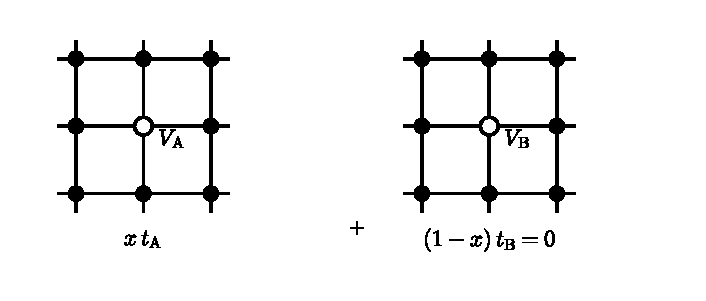
\includegraphics[width=8.5cm]{fig12-2.pdf}\\{\small 图 12.2\quad 二元无序合金中单格点近似的相干势近似的自洽方程图示（其中●组成待定的有效介质）}
\end{minipage}
\end{center}

再看无序系统的自能，在单格点近似时系统相对于有效介质的自能，可根据式(12.2.28)，写为
\begin{equation}
  \Sigma_{1}\left(\omega\right)=\frac{\langle t_{i}\rangle}
  {1+\mathscr{F}\left(\omega\right)\langle t_{i}\rangle}
\end{equation}
由 $\Sigma_{1}$ 构成的自能矩阵满足
\begin{equation}
  \hat{\boldsymbol{\Sigma}}_{1}=\hat{\boldsymbol{P}}^{-1}-\langle\hat{\boldsymbol{G}}\rangle^{-1}
\end{equation}
无序合金系统的自能矩阵则满足
\begin{equation}
  \hat{\boldsymbol{\Sigma}}=\hat{\boldsymbol{G}}_{0}^{-1}-\langle\hat{\boldsymbol{G}}\rangle^{-1}
\end{equation}
其中 $G_{0}$ 是 $H_{0}$ 的格林函数，不包括相干势 $u\left(\omega\right)$［见式(12.3.10)］.由于 $\hat{\boldsymbol{G}}_{0}^{-1}=\left(\omega\hat{\boldsymbol{I}}-\hat{\boldsymbol{H}}_{0}\right)$，而 $\hat{\boldsymbol{P}}^{-1}=\left(\omega\hat{\boldsymbol{I}}-\hat{\boldsymbol{H}}_{0}-u\hat{\boldsymbol{I}}\right)$.根据式(12.3.25)与式(12.3.26)，易求出 $\hat{\boldsymbol{\Sigma}}-\hat{\boldsymbol{\Sigma}}_{1}=u\left(\omega\right)\hat{\boldsymbol{I}}$.因此二元合金系统在单格点近似时的CPA自能为
\begin{equation}
  \Sigma\left(\omega\right)=u\left(\omega\right)+\Sigma_{1}\left(\omega\right)
\end{equation}
从 $\Sigma_{1}\left(\omega\right)$ 的表示式可知，当 $\langle t_{i}\left[u\left(\omega\right)\right]\rangle=0$ 时，$\Sigma_{1}\left(\omega\right)=0$.最后求得简单关系式
\begin{equation}
  \Sigma\left(\omega\right)=u\left(\omega\right)
\end{equation}
这是由于无序系统相对于有效介质的平均散射为零，因此有效介质的自能 $u\left(\omega\right)$ 就是无序系统的自能.相干势近似的成功就在于可以自洽决定相干势 $u\left(\omega\right)$，而 $u\left(\omega\right)$ 有自洽解则表明有效介质（或参考晶体）可以用一种规范的方法来自洽地确定，这就克服了平均t矩阵近似法不能自洽确定参考晶体的缺点.然而在相干势近似计算中，为了求得良好的近似解，从输入 $u\rightarrow$ 计算 $\mathscr{F}\left(\omega\right)\rightarrow$ 满足 $\langle t_{i}\rangle=0$ 条件往往需要多次反复进行，直至 $u\left(\omega\right)$ 满足相干势近似自洽方程式(12.3.21)为止.但是，这类自洽计算是可行的，因为在某些极限下系统有严格解.例如，在二元合金中当浓度 $x\rightarrow0$ 或 $x\rightarrow1$ 时，都可以找到严格解或良好近似解.

\subsection*{3. 简短结语}

相干势近似的中心思想是：将无规势用一个与频率 $\omega$ 有关，但具平移不变性的有效介质的相干势 $u\left(\omega\right)$ 来代替，后者由自洽条件决定.在单格点近似的CPA中，自洽条件要求无序系统与有效介质之间的散射t矩阵逐点平均为零，仅当此条件满足时才可求得如下重要结论：

（i）无规平均的格点格林函数等于有效介质的格林函数；

（ii）系统的自能就是有效介质的相干势.这时有效介质才是良好选择的.

无序系统中准粒子的态密度由无规平均格林函数的虚部决定
\begin{equation*}
  \rho\left(\omega\right)=-\left(1/\pi\right)\mathrm{Im}\left\{\left(1/N\right)\mathrm{Tr}\langle\hat{\boldsymbol{G}}\left(\omega+\mathrm{i}\eta\right)\rangle\right\}
\end{equation*}

{\sloppy
在相干势近似中，当 $\langle\hat{T}\rangle=0$ 时 $\langle\hat{\boldsymbol{G}}\rangle=\hat{\boldsymbol{P}}$，又因为 $\left(1/N\right)\mathrm{Tr}\left(\hat{\boldsymbol{P}}\right)=\mathscr{F}\left(\omega\right)$ $=\left(1/N\right)\sum_{k}\left[\omega-\varepsilon_{k}-u\left(\omega\right)\right]^{-1}$，这时准粒子的态密度简化为计算 $\mathscr{F}\left(\omega+\mathrm{i}\eta\right)$ 的虚部\par}
\begin{equation}
  \rho\left(\omega\right)=-\frac{1}{\pi}\mathrm{Im}\,\mathscr{F}\left(\omega+\mathrm{i}\eta\right)
\end{equation}
但应注意，在 $\mathscr{F}$ 中隐含相干势 $u\left(\omega\right)$，因此 $\mathscr{F}\left(\omega\right)$ 实际上代表 $\mathscr{F}\left[u\left(\omega\right)\right]$.相干势近似的自洽计算主要归结为求无序系统中准粒子的态密度 $\rho\left(\omega\right)$，并由此得知有关的热力学量.

相干势近似法不仅适用于在 $0<x<1$ 全浓度区求解成分（或替代）无序系统，它还因计入了多重散射效应可用于强散射体系.米泽曾对相干势近似方法作了详细的评述，有兴趣的读者可参阅文献[1].相干势近似已成为处理成分无序系统的一种行之有效的方法.在下节中，将介绍处理强关联电子系统的隶玻色子平均场近似法是如何被我们推广到无序系统的，并与相干势近似法相结合构成一个描述无序重费密子系统的强关联相干势近似理论\textsuperscript{[4,5]}.

\section{无序重费密子系统的相干势近似理论}

重费密子系统是每个元胞中均含局域f电子的晶格与传导电子的相互作用系统，其中同格点上f电子的强库仑排斥（即强关联）作用导致局域化，这是固体中首先涉及强关联电子体系的一个范例.正如上章中所指出重费密子系统包括金属与绝缘体两种情形，分别称为重费密子金属（如 $\mathrm{CeAl}_{3}$）和近藤绝缘体（如 $\mathrm{Ce}_{3}\mathrm{Bi}_{4}\mathrm{Pt}_{3}$），在理论上均可用安德逊晶格模型（ALM）描述.重费密子金属与近藤绝缘体的低温特性可运用处理强关联的隶玻色子平均场近似方法求解，并已在上章的§7与§8中作了详细的介绍.在本节中我们将讨论用La（无f电子）替代Ce（有f电子）所构成的无序重费密子系统，如重费密子合金 $\left(\mathrm{La}_{x}\mathrm{Ce}_{1-x}\right)\mathrm{Al}_{3}$ 和掺杂近藤绝缘体 $\left(\mathrm{La}_{x}\mathrm{Ce}_{1-x}\right)_{3}\mathrm{Bi}_{4}\mathrm{Pt}_{3}$ 等成分无序系统的CPA理论.

\subsection*{1. 重费密子系统的无序模型}

可将无序重费密子系统 $\left(\mathrm{La}_{x}\mathrm{Ce}_{1-x}\right)\mathrm{Al}_{3}$ 和 $\left(\mathrm{La}_{x}\mathrm{Ce}_{1-x}\right)_{3}\mathrm{Bi}_{4}\mathrm{Pt}_{3}$ 中的 $\left(\mathrm{La}_{x}\mathrm{Ce}_{1-x}\right)$ 部分看成二元无序合金 $\mathrm{A}_{x}\mathrm{B}_{1-x}$，其中A原子类La（不含f电子），B原子类Ce（含有f电子），其它部分仅提供传导电子并构成含f和c电子的无序系统.理论上相当于在安德逊晶格中的f部分引进成分无序.为此，定义i格点的无规变量
\begin{equation}
  \xi_{i}=\begin{cases}1 & \left(l\in\mathrm{A}\right)\\ 0 & \left(l\in\mathrm{B}\right)\end{cases}
\end{equation}
并注意到 $\xi_{i}$ 的无规平均 $\overline{\xi}_{i}^{2}=\overline{\xi}_{i}=x$，这里x代表合金中A原子的归一浓度.按此，可写出无序重费密子系统的出发哈密顿量
\begin{equation}
\begin{aligned}
  H&=\sum_{k,\sigma}\varepsilon_{k}C_{k\sigma}^{+}C_{k\sigma}
  +\sum_{i,\sigma}\left[\xi_{i}E_{\mathrm{L}}+\left(1-\xi_{i}\right)E_{0}\right]n_{i\sigma}^{f}
  +U\sum_{i}\left(1-\xi_{i}\right)n_{i\uparrow}^{f}n_{i\downarrow}^{f}\\
  &\quad+V\sum_{i,\sigma}\left(1-\xi_{i}\right)
  \left(C_{i\sigma}^{+}f_{i\sigma}+f_{i\sigma}^{+}C_{i\sigma}\right)
\end{aligned}
\end{equation}
其中 $n_{i\sigma}^{f}=f_{i\sigma}^{+}f_{i\sigma}$，$\varepsilon_{k}$ 为传导电子的能量，$E_{0}$ 是B原子上f电子的未微扰能级，它远在费密能级之下.$E_{\mathrm{L}}$ 代表A原子的f能级，为确保A上无f电子占据（类似La），在具体计算时应取 $E_{\mathrm{L}}\rightarrow\infty$.此外，V为安德逊c-f杂化参数，而U则是同一格点上自旋取向相反的f电子之间的库仑关联作用，这两项都只出现在被B原子（类Ce）占据的格点上.由于重费密子系统属于 $U\rightarrow\infty$ 强关联情形，这时B原子格点上f电子的双占据态将被严格排除，f电子的占据数只能取0或1，因此式中含U项将不出现.这时强关联效应可以通过在含V的杂化项中引入隶玻色子场算符 $b_{i}$ 并加上约束条件 $b_{i}^{+}b_{i}+\sum_{\sigma}f_{i\sigma}^{+}f_{i\sigma}=1$（其中 $i\in\mathrm{B}$）而严格计入.类似于上章§7中的讨论，作隶玻色子的平均场近似（SBMFA），引入隶玻色子的平均场参量 $\langle b_{i}\rangle=\langle b_{i}^{+}\rangle=r$ 和平均约束 $\lambda\sum_{i}\left(1-\xi_{i}\right)\left(r^{2}+\sum_{\sigma}f_{i\sigma}^{+}f_{i\sigma}-1\right)$，将SBMFA的无序哈密顿量写为
\begin{equation}
\begin{aligned}
  H_{\mathrm{MF}}&=\sum_{k\sigma}\varepsilon_{k}C_{k\sigma}^{+}C_{k\sigma}
  +\sum_{i\sigma}\left[\xi_{i}E_{\mathrm{L}}+\left(1-\xi_{i}\right)E_{0}\right]f_{i\sigma}^{+}f_{i\sigma}\\
  &\quad+rV\sum_{i\sigma}\left(1-\xi_{i}\right)
  \left(C_{i\sigma}^{+}f_{i\sigma}+f_{i\sigma}^{+}C_{i\sigma}\right)\\
  &\quad+\lambda\sum_{i}\left(1-\xi_{i}\right)
  \left(r^{2}+\sum_{\sigma}f_{i\sigma}^{+}f_{i\sigma}-1\right)
\end{aligned}
\end{equation}
注意在 $H_{\mathrm{MF}}$ 中无规变量 $\xi_{i}$ 既出现在f电子的格点能中，也出现在c-f杂化项中，这是一个既含“对角”又有“非对角”无序的系统.稍作整理可将 $H_{\mathrm{MF}}$ 中的无规部分写成下列（$2\times2$）矩阵表示：
\begin{equation}
\begin{aligned}
  H_{\mathrm{MF}}=\sum_{i,\sigma}\Bigl\{&\left(1-\xi_{i}\right)\left[C_{i\sigma}^{+}\ \ f_{i\sigma}^{+}\right]
  \begin{pmatrix}0 & rV\\ rV & E_{f}\end{pmatrix}
  \begin{pmatrix}C_{i\sigma}\\ f_{i\sigma}\end{pmatrix}\\
  &+\xi_{i}\left[C_{i\sigma}^{+}\ \ f_{i\sigma}^{+}\right]
  \begin{pmatrix}0 & 0\\ 0 & E_{\mathrm{L}}\end{pmatrix}
  \begin{pmatrix}C_{i\sigma}\\ f_{i\sigma}\end{pmatrix}\Bigr\}\\
  &+\sum_{k,\sigma}\varepsilon_{k}C_{k\sigma}^{+}C_{k\sigma}
  +\lambda\left(r^{2}-1\right)\left(1-x\right)N
\end{aligned}
\end{equation}
其中 $E_{f}=E_{0}+\lambda$ 代表f电子的重整能级，而SBMFA参量 $\lambda$ 与 $r$ 在i格点被B（类Ce）原子占据时满足与式(11.7.25)类似的自洽方程
\begin{equation}
  \left.
  \begin{aligned}
    r\lambda&=-V\sum_{\sigma}\ \langle C_{i\sigma}^{+}f_{i\sigma}\rangle\\
    1-r^{2}&=n_{f}=\sum_{\sigma}\ \langle f_{i\sigma}^{+}f_{i\sigma}\rangle
  \end{aligned}
  \right\}i\in\mathrm{B}
\end{equation}
在具体运算时，还需要作无规平均.

\subsection*{2. 有效介质}

由于 $H_{\mathrm{MF}}$ 中既含对角无序，又有非对角无序，并且可以用（$2\times2$）矩阵表示，应当引入下列（$2\times2$）的相干势作为有效介质的合理描述：
\begin{equation}
  S\left(\omega,x\right)=
  \begin{pmatrix}S_{\mathrm{cc}} & S_{\mathrm{cf}}\\ S_{\mathrm{fc}} & S_{\mathrm{ff}}\end{pmatrix}
\end{equation}
其中 $S\left(\omega,x\right)$ 与格点位置无关，这是一个具有平移对称性的待定函数，相干势矩阵的诸元素也与i无关，最多只是 $\omega$ 及x的函数.由此可写出有效介质的平均场哈密顿量
\begin{equation}
\begin{aligned}
  \overline{H}=\sum_{i,\sigma}\left[C_{i\sigma}^{+}\ \ f_{i\sigma}^{+}\right]
  &\begin{pmatrix}S_{\mathrm{cc}} & S_{\mathrm{cf}}\\ S_{\mathrm{fc}} & E_{f}+S_{\mathrm{ff}}\end{pmatrix}
  \begin{pmatrix}C_{i\sigma}\\ f_{i\sigma}\end{pmatrix}\\
  &+\sum_{k,\sigma}\varepsilon_{k}C_{k\sigma}^{+}C_{k\sigma}
  +\lambda\left(r^{2}-1\right)\left(1-x\right)N
\end{aligned}
\end{equation}
作傅里叶变换，可将这个待定的有效介质哈密顿量用布洛赫表象中算符表示
\begin{equation}
  \overline{H}=\sum_{k,\sigma}\left[C_{k\sigma}^{+}\ \ f_{k\sigma}^{+}\right]
  \begin{pmatrix}\varepsilon_{k}+S_{\mathrm{cc}} & S_{\mathrm{cf}}\\ S_{\mathrm{fc}} & E_{f}+S_{\mathrm{ff}}\end{pmatrix}
  \begin{pmatrix}C_{k\sigma}\\ f_{k\sigma}\end{pmatrix}
  +\lambda\left(r^{2}-1\right)\left(1-x\right)N
\end{equation}
将用于计算有效介质的平均格点格林函数.

现在讨论重费密子系统的相干势近似问题，首先由无序的 $H_{\mathrm{MF}}$ 与有效介质的 $\overline{H}$ 之差定义无规势
\begin{equation}
  H_{\mathrm{MF}}-\overline{H}\equiv\sum_{i}V_{i}
\end{equation}
对于二元无序合金，无规势只取两个分立值 $V_{\mathrm{A}}$ 和 $V_{\mathrm{B}}$，分别对应于取 $\xi_{i}$=1和0.根据式(12.4.4)和式(12.4.7)求得
\begin{equation}
  V_{\mathrm{A}}=
  \begin{pmatrix}-S_{\mathrm{cc}} & -S_{\mathrm{cf}}\\ -S_{\mathrm{fc}} & \varepsilon_{\mathrm{L}}-S_{\mathrm{ff}}\end{pmatrix},
  \qquad
  V_{\mathrm{B}}=
  \begin{pmatrix}-S_{\mathrm{cc}} & rV-S_{\mathrm{cf}}\\ rV-S_{\mathrm{fc}} & -S_{\mathrm{ff}}\end{pmatrix}
\end{equation}
在上式中 $\varepsilon_{\mathrm{L}}\equiv E_{\mathrm{L}}-E_{f}$，计算时可直接取 $\varepsilon_{\mathrm{L}}\rightarrow\infty$，它等效于 $E_{\mathrm{L}}\rightarrow\infty$.因为在上章§8中已证明：零温时，$E_{f}-\mu=k_{\mathrm{B}}T_{\mathrm{L}}$ 为小量，当取费密能（即零温化学势 $\mu$）为能量的原点时，有 $k_{\mathrm{B}}T_{\mathrm{L}}\ll E_{\mathrm{L}}$，这时 $\varepsilon_{\mathrm{L}}\rightarrow\infty$ 同样是保证A原子上无f电子的条件.根据式(12.2.26)，即可写出A、B原子在有效介质背景上的散射t矩阵
\begin{equation}
  t_{\mathrm{A}(\mathrm{B})}=V_{\mathrm{A}(\mathrm{B})}
  \left[1-F\left(\omega\right)V_{\mathrm{A}(\mathrm{B})}\right]^{-1}
\end{equation}
由此构成单格点近似的CPA自洽方程
\begin{equation}
  xt_{\mathrm{A}}+\left(1-x\right)t_{\mathrm{B}}=0
\end{equation}
其中 $F\left(\omega\right)$ 代表有效介质 $\overline{H}$ 的平均格点格林函数，可利用式(12.4.8)求出为
\begin{equation}
\begin{aligned}
  F\left(\omega\right)&=\frac{1}{N}\sum_{k}\overline{G}\left(\omega,\boldsymbol{k}\right)
  =\begin{pmatrix}F_{\mathrm{cc}} & F_{\mathrm{cf}}\\ F_{\mathrm{fc}} & F_{\mathrm{ff}}\end{pmatrix}\\
  &=\frac{1}{N}\sum_{k}
  \frac{\begin{pmatrix}\omega-E_{f}-S_{\mathrm{ff}} & S_{\mathrm{cf}}\\ S_{\mathrm{fc}} & \omega-\varepsilon_{k}-S_{\mathrm{cc}}\end{pmatrix}}
  {\left[\left(\omega-E_{f}-S_{\mathrm{ff}}\right)\left(\omega-\varepsilon_{k}-S_{\mathrm{cc}}\right)-S_{\mathrm{cf}}S_{\mathrm{fc}}\right]}
\end{aligned}
\end{equation}
当相干势 $S_{\mathrm{cc}}$、$S_{\mathrm{cf}}$、$S_{\mathrm{fc}}$ 和 $S_{\mathrm{ff}}$ 满足相干势近似自洽方程式(12.4.12)时，有效介质的格林函数 $\left[F\left(\omega\right)\right]$ 就是重费密子系统的无规平均格林函数.

\subsection*{3. 相干势的解}

联立式(12.4.10-13)，并取 $\varepsilon_{\mathrm{L}}\rightarrow\infty$ 条件后，经直接运算可证明在相干势矩阵 $S\left(\omega,x\right)$ 中有3个元素存在简单的解析解\textsuperscript{[4]}：
\begin{equation}
  S_{\mathrm{cc}}=0,\qquad S_{\mathrm{cf}}=S_{\mathrm{fc}}=rV
\end{equation}
只有 $S_{\mathrm{ff}}\left(\omega,x\right)$ 必须通过数值计算自洽求解.因此，相干势矩阵简化为
\begin{equation}
  S\left(\omega,x\right)=
  \begin{pmatrix}0 & rV\\ rV & S_{\mathrm{ff}}\left(\omega,x\right)\end{pmatrix}
\end{equation}
再将此解代入式(12.4.10)、(12.4.11)并取 $\varepsilon_{\mathrm{L}}\rightarrow\infty$，又可求出A、B原子相对有效介质的t矩阵解
\begin{equation}
  t_{\mathrm{A}}=\frac{1}{F_{\mathrm{ff}}\left(\omega\right)}
  \begin{pmatrix}0 & 0\\ 0 & -1\end{pmatrix},
  \qquad
  t_{\mathrm{B}}=\frac{S_{\mathrm{ff}}\left(\omega,x\right)}
  {1+S_{\mathrm{ff}}\left(\omega,x\right)F_{\mathrm{ff}}\left(\omega\right)}
  \begin{pmatrix}0 & 0\\ 0 & -1\end{pmatrix}
\end{equation}
最后，将 $t_{\mathrm{A}}$、$t_{\mathrm{B}}$ 解代入单格点近似的CPA自洽方程式(12.4.12)，求得简化的相干势近似自洽方程
\begin{equation}
  S_{\mathrm{ff}}\left(\omega,x\right)F_{\mathrm{ff}}\left(\omega\right)=-x
\end{equation}
其中与相干势 $S_{\mathrm{ff}}$ 同时自洽确定的 $F_{\mathrm{ff}}\left(\omega\right)$ 是f电子的平均格点格林函数
\begin{equation}
  F_{\mathrm{ff}}\left(\omega\right)=\frac{1}{N}\sum_{k}
  \frac{\left(\omega-\varepsilon_{k}\right)}
  {\left[\left(\omega-\varepsilon_{k}\right)\left(\omega-E_{f}-S_{\mathrm{ff}}\right)-\left(rV\right)^{2}\right]}
\end{equation}
由于我们找出了相干势的简单解式(12.4.15)，（$2\times2$）的相干势近似方程简化为仅仅求解一个未知相干势分量 $S_{\mathrm{ff}}$ 的问题，将使自洽计算的工作量明显减小.对应于相干势的简单解，$F\left(\omega\right)$ 矩阵的其它分量均可写成下列表示式：
\begin{equation}
  F_{\mathrm{cc}}\left(\omega\right)=\left(1/N\right)\sum_{k}
  \frac{\left(\omega-E_{f}-S_{\mathrm{ff}}\right)}
  {\left[\left(\omega-\varepsilon_{k}\right)\left(\omega-E_{f}-S_{\mathrm{ff}}\right)-\left(rV\right)^{2}\right]}
\end{equation}
\begin{equation}
  F_{\mathrm{fc}}\left(\omega\right)=F_{\mathrm{cf}}\left(\omega\right)
  =\frac{\left(rV\right)}{\left(\omega-E_{f}-S_{\mathrm{ff}}\right)}F_{\mathrm{cc}}\left(\omega\right)
\end{equation}
此外，无序重费密子系统的SBMFA参量 $\lambda$ 和 $r$ 所满足的方程式(12.4.5)经无规平均后，按照格林函数的谱定理，可用有效介质的平均格点格林函数表示为
\begin{equation}
  \left(1-x\right)r\lambda=\left(2/\pi\right)V\int_{-\infty}^{\infty}
  f\left(\omega-\mu\right)\mathrm{Im}\,F_{\mathrm{fc}}\left(\omega+\mathrm{i}\eta\right)\mathrm{d}\omega
\end{equation}
\begin{equation}
  \left(1-x\right)\left(1-r^{2}\right)=-\left(2/\pi\right)\int_{-\infty}^{\infty}
  f\left(\omega-\mu\right)\mathrm{Im}\,F_{\mathrm{ff}}\left(\omega+\mathrm{i}\eta\right)\mathrm{d}\omega
\end{equation}
其中 $f\left(\omega-\mu\right)$ 是费密分布函数，$\mu$ 为化学势，由总粒子数确定.设平均每格点的总电子浓度为 $n_{\mathrm{t}}=n_{\mathrm{c}}+n_{\mathrm{f}}$，其中 $n_{\mathrm{c}}$ 是传导电子的浓度，而f电子浓度在二元合金中为 $n_{\mathrm{f}}=\left(1-x\right)$.因此
\begin{equation}
\begin{aligned}
  n_{\mathrm{t}}=n_{\mathrm{c}}+\left(1-x\right)
  &=-\left(2/\pi\right)\int_{-\infty}^{\infty}\mathrm{d}\omega\,f\left(\omega-\mu\right)\\
  &\quad\times\mathrm{Im}\left[F_{\mathrm{cc}}\left(\omega+\mathrm{i}\eta\right)
  +F_{\mathrm{ff}}\left(\omega+\mathrm{i}\eta\right)\right]
\end{aligned}
\end{equation}
式(12.4.17)—(12.4.23)构成同时自洽决定无序重费密子系统的相干势 $S_{\mathrm{ff}}$，隶玻色子平均场参量r与 $\lambda$，以及化学势 $\mu$ 等未知量的基本方程组.此外，它还便于计算任意掺杂浓度x时的电子态密度.

\subsection*{4. 无序重费密子系统的电子态密度}

当自旋取向一定时，平均每个格点的传导电子态密度c-DOS由 $F_{\mathrm{cc}}\left(\omega+\mathrm{i}\eta\right)$ 的虚部直接决定
\begin{equation}
  \rho_{\mathrm{c}}\left(\omega,x\right)=-\left(1/\pi\right)\mathrm{Im}\,F_{\mathrm{cc}}\left(\omega+\mathrm{i}\eta\right)
  \qquad\left(\eta=0^{+}\right)
\end{equation}
而f-DOS表示平均每个B（类Ce）原子在确定自旋取向时的f电子态密度，它应由 $F_{\mathrm{ff}}\left(\omega+\mathrm{i}\eta\right)$ 的虚部决定
\begin{equation}
  \rho_{\mathrm{f}}\left(\omega,x\right)
  =-\left[1/\left(1-x\right)\pi\right]\mathrm{Im}\,F_{\mathrm{ff}}\left(\omega+\mathrm{i}\eta\right)
  \qquad\left(\eta=0^{+}\right)
\end{equation}
其中 $F_{\mathrm{ff}}$ 和 $F_{\mathrm{cc}}$ 由公式(12.4.18)，(12.4.19)决定.在计算时涉及将对k求和化为对能量的积分，还应给出传导电子的未微扰态密度
\begin{equation}
  \rho_{0}\left(\omega\right)=\left(1/N\right)\sum_{k}\delta\left(\omega-\varepsilon_{k}\right)
\end{equation}
{\sloppy
的具体形式.通常为方便起见，可取导带半宽为D的矩形态密度：$\rho_{0}\left(\omega\right)=\left(1/2D\right)$ $\left(|\omega|<D\right)$，$\rho_{0}\left(\omega\right)=0$ $\left(|\omega|>D\right)$.有时为表现细致特征，需采用更为合理的赫伯德型态密度：$\rho_{0}\left(\omega\right)=\left(2/\pi D\right)\left[1-\left(\omega/D\right)^{2}\right]^{1/2}$ $\left(|\omega|<D\right)$，$\rho_{0}\left(\omega\right)=0$ $\left(|\omega|>D\right)$.以上是无序重费密子系统中相干势近似理论的基本框架.\par}

在文献中常用未掺杂（即 $x=0$）时安德逊晶格中 $n_{\mathrm{c}}<1$ 或 $n_{\mathrm{c}}=1$ 而将有序的重费密子系统划分为重费密子金属和近藤绝缘体两大类：这种分类也被推广到无序体系，人们将 $n_{\mathrm{c}}<1$ 情形称为重费密子合金，而 $n_{\mathrm{c}}=1$ 情况则叫掺杂近藤绝缘体.对于掺杂近藤绝缘体系统，x代表掺入的类La原子（无f电子）浓度，由于用类La原子替代类Ce原子（有f电子）将产生缺少f电子的中心，形成近藤空穴，因此x又可称为近藤空穴的浓度.1994年我们应用上述相干势近似理论计算了掺杂近藤绝缘体系统中f-DOS随x的演化\textsuperscript{[4]}，结果表明：当未掺杂 $\left(x=0\right)$ 时，近藤绝缘体中在费密能级处存在如图11.15所示的非直接能隙，少量掺近藤空穴会在能隙的中央自然形成“隙间杂质带”，在中等掺杂时 $\left(x>10\%\mathrm{La}\right)$，能隙将被逐渐抹平，代之以双峰型的赝隙，表明系统已具有金属性.此结果可用于解释掺杂时随着x的增加，系统从近藤绝缘体向重费密子金属逐渐演变的实验现象.将此理论用于重费密子合金也对其低温相干特性作出了合理的说明\textsuperscript{[5]}.

在结束本节之前还需强调指出：无序重费密子系统不仅是强关联电子系统，而且还涉及强散射情形.这是因为用不含f电子的La取代含有f电子的Ce所形成的近藤空穴具有很高的能量 $\left(E_{\mathrm{L}}\rightarrow\infty\right)$，它远远高于Ce原子上f电子的能量 $\left(E_{\mathrm{L}}\gg|E_{0}|\right)$.因此，每个近藤空穴都是非常强的散射源，这时无序重费密子系统已不能用低阶玻恩近似作微扰处理，必须采用相干势近似，才能计入强散射源所导致的多重散射效应.这就是我们在SBMFA基础上构造相干势近似理论的初衷，在相关的文献中被称为推广的隶玻色子理论.

\section{无序系统中的电子态}

\subsection*{1. 安德逊的无序模型}

先定性介绍有序晶体与无序系统电子能态特征的主要区别.

具有严格周期性的有序晶格是平移不变的，单电子态可用波矢量 $\boldsymbol{k}$ 标记并形成能带，能带电子的状态由布洛赫函数表示
\begin{equation*}
  \psi_{\boldsymbol{k}}\left(\boldsymbol{r}\right)=u_{\boldsymbol{k}}\left(\boldsymbol{r}\right)\mathrm{e}^{\mathrm{i}\boldsymbol{k}\cdot\boldsymbol{r}}
\end{equation*}
所有的电子均在有序晶格中作公有化运动，且各格点周围振幅 $u_{\boldsymbol{k}}\left(\boldsymbol{r}\right)$ 相同，这种状态在整个晶体中的扩展特征是长程序效应的反映，因此布洛赫态又可称为扩展态（extended states）.具有扩展态是有序晶格的特点.

当有序晶格中（如半导体）掺入少量杂质后，周期性被局部破坏，正如第八章中讨论所指出，这时将有电子或空穴被束缚在杂质上，并在导带之下或价带之上（能隙区中）形成施主和受主能级，这些电子（或空穴）的波函数是指数衰减型的定域函数
\begin{equation*}
  \psi\left(\boldsymbol{r}\right)\sim\exp\left(-r/\zeta\right)
\end{equation*}
$\zeta$ 称为定域化长度.这时电子在杂质附近作定域化的运动，有别于扩展在整个晶体中的公有化运动，称为电子的定域态（localized states，又称局域态）.实验表明当杂质浓度增高时，定域态的电子能级可能密集成带，并与导带相连接，形成导带的尾部（tail），它们对电导率的贡献很小\textsuperscript{[6]}.由此可知存在定域态是无序的标志.

对于无序系统的电子态理论研究有两种处理方法：其一是对无序系统作某种平均后近似当作有序系统来处理，这种方法以相干势近似为代表.其二，则相反的从无序系统的定域态特点出发，设计一些无序模型，研究无序系统与有序系统电子态的差别，这种方法以安德逊的工作为代表，最简单的介绍可参考李雅达的报告\textsuperscript{[7]}.我们将用比文献[7]稍为严格一些的方法介绍安德逊工作，首先引进安德逊的无序模型.

与有序晶格不同，无序系统由于不具有平移对称性，波矢量 $\boldsymbol{k}$ 不再是描述电子状态的好量子数，我们必须从定域态（或原子轨道态）出发设计模型和讨论问题.安德逊将紧束缚近似（TBA）方法推广用于无序系统，设单电子哈密顿量为
\begin{equation}
  H=-\frac{\hbar^{2}}{2m}\nabla^{2}+V\left(\boldsymbol{r}\right)
\end{equation}
取瓦尼尔函数 $a\left(\boldsymbol{r}-\boldsymbol{l}\right)$ 为基，将二次量子化态向量表示成
\begin{equation*}
  \Psi\left(\boldsymbol{r}\right)=\sum_{l}C_{l}\,a\left(\boldsymbol{r}-\boldsymbol{l}\right)
\end{equation*}
则H可改写为
\begin{equation}
  H=\sum_{l}\mathscr{E}_{l}C_{l}^{+}C_{l}+\sum_{l\neq l'}\ \sum_{l'}V_{ll'}C_{l}^{+}C_{l'}
\end{equation}
其中
\begin{equation}
  \mathscr{E}_{l}\equiv H_{ll}=\int a^{*}\left(\boldsymbol{r}-\boldsymbol{l}\right)
  Ha\left(\boldsymbol{r}-\boldsymbol{l}\right)\mathrm{d}\tau
\end{equation}
代表l格点附近定域电子能量，而 $V_{ll'}$ 就是交迭积分
\begin{equation}
  V_{ll'}\equiv H_{ll'}=\int a^{*}\left(\boldsymbol{r}-\boldsymbol{l}\right)
  Ha\left(\boldsymbol{r}-\boldsymbol{l}'\right)\mathrm{d}\tau
\end{equation}
在TBA范围内 $V_{ll'}=V_{l}\delta_{l',l+h}$，$\boldsymbol{h}$ 为近邻格点间位置矢差，$V_{l}$ 代表l格点处电子的近邻交迭积分.

当系统为有序晶格时，由于具有平移对称性可引入波矢 $\boldsymbol{k}$ 描述电子状态，并利用布洛赫定理得到 $C_{k}$ 与 $C_{l}$ 的关系为
\begin{equation}
  C_{l}=\frac{1}{\sqrt{N}}\sum_{k}\mathrm{e}^{\mathrm{i}\boldsymbol{k}\cdot\boldsymbol{l}}C_{k}
\end{equation}
这个关系只适用于有序或近似有序的晶格.另外，由于平移对称各格点的 $\mathscr{E}_{l}$ 及 $V_{l}$ 均与l无关，可令 $\mathscr{E}_{l}=\mathscr{E}_{0}$ 以及 $V_{l}=V$，式(12.5.4)简化为
\begin{equation}
  V_{ll'}=V\delta_{l',l+h}
\end{equation}
V代表近邻交迭积分.系统的哈密顿量简化为 $C_{k}$ 的对角形式
\begin{equation}
\begin{aligned}
  H&=\mathscr{E}_{0}\sum_{l}C_{l}^{+}C_{l}
  +V\sum_{l}\ \sum_{h}C_{l}^{+}C_{l+h}\\
  &=\sum_{k}E\left(\boldsymbol{k}\right)C_{k}^{+}C_{k}
\end{aligned}
\end{equation}
其中
\begin{equation}
  E\left(\boldsymbol{k}\right)=\mathscr{E}_{0}+V\sum_{h}\mathrm{e}^{\mathrm{i}\boldsymbol{k}\cdot\boldsymbol{h}}
\end{equation}
这就是TBA的能带电子能量，其能带宽度等于 $2Z|V|$，Z是配位数.若取带中心能量 $\mathscr{E}_{0}$ 为原点，则有序晶格的电子态能量
\begin{equation}
  E\left(\boldsymbol{k}\right)=V\sum_{h}\mathrm{e}^{\mathrm{i}\boldsymbol{k}\cdot\boldsymbol{h}}
\end{equation}
相当于令 $\mathscr{E}_{0}=0$.

对于无序系统，$\mathscr{E}_{l}$ 将随格点l作随机变化，这时不能再令 $\mathscr{E}_{l}=0$，安德逊假定 $\mathscr{E}_{l}$ 在W宽度内是连续均匀分布的，各格点上的 $\mathscr{E}_{l}$ 是独立无规变量，其分布概率为
\begin{equation}
  P\left(\mathscr{E}_{l}\right)=
  \begin{cases}
    \dfrac{1}{W} & \left(|\mathscr{E}_{l}|\leqslant\dfrac{W}{2}\right)\\[0.8em]
    0 & \left(|\mathscr{E}_{l}|>\dfrac{W}{2}\right)
  \end{cases}
\end{equation}
如图12.3所示.对于近邻交迭积分，假设它仍与l无关由V表示，式(12.5.6)仍然适用，这就是安德逊设计的无序模型.在安德逊模型中哈密顿量写成
\begin{equation}
  H=\sum_{l}\mathscr{E}_{l}C_{l}^{+}C_{l}
  +V\sum_{l}\ \sum_{h}C_{l}^{+}C_{l+h}
\end{equation}

\begin{center}
\begin{minipage}{6cm}
\centering
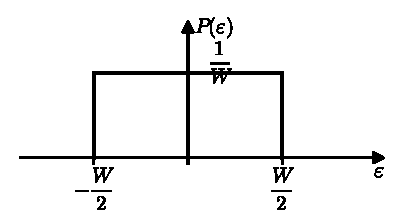
\includegraphics[width=6cm]{fig12-3.pdf}\\{\small 图 12.3}
\end{minipage}
\end{center}

其中无规变量是 $\mathscr{E}_{l}$，它的变化宽度W可当作反映系统“无序程度”的参量，而各格点的近邻交迭积分均取相同值V则表示无序系统的“短程有序”特性.因此，这个简化的模型概括了无序系统的主要特点.由此出发将便于求得定域化条件和引进迁移率边界等新概念.

\subsection*{2. 安德逊定域化\textsuperscript{[8]}}

安德逊首先对无序系统中的电子定域态和扩展态作了严格定义.他指出，在无限大的体系中\footnote{由于无序系统不存在平移对称性，人们不必像有序晶体那样去设计周期性边界条件，以保证有限晶体的平移对称性，而是直接讨论无限大样品的热力学极限（$N\rightarrow\infty$，$V\rightarrow\infty$ 和 $N/V=$ 有限）.}设 $t=0$ 时l格上（或其附近）有一个电子，那么经过较长时间t以后在l格点上如果找到这个电子的概率振幅 $A_{l}\left(t\right)$ 为零，就说明电子离开了这个格点在系统中传播，电子处于扩展态；如果 $A_{l}\left(t\right)\neq0$（t很大），就表示电子在l格点附近形成了稳定的定域态，这就是安德逊的定域化概念.

安德逊详细讨论了这个含时问题，得到的结论是：对于三维无序系统，当无规起伏势能的分布宽度W与带宽2ZV之比 $\delta$ 大于某个临界值 $\delta_{\mathrm{c}}$ 时，无序系统中所有的本征态都是定域态，$\delta_{\mathrm{c}}$ 的数值大致等于2.

利用 $C_{l}$ 及 $C_{l'}^{+}$ 所组成的双时推迟格林函数
\begin{equation}
  G_{ll'}\left(t\right)\equiv-\mathrm{i}\theta\left(t\right)
  \langle\left[C_{l}\left(t\right),\,C_{l'}^{+}\left(0\right)\right]_{+}\rangle
\end{equation}
讨论安德逊模型是方便的.当 $T=0$ K时上式简化为对基态的平均
\begin{equation}
  G_{ll'}\left(t\right)=-\mathrm{i}\theta\left(t\right)
  \langle0|C_{l}\left(t\right)C_{l'}^{+}\left(0\right)|0\rangle
\end{equation}
这个函数的对角部分 $G_{ll}\left(t\right)$ 直接与 $A_{l}\left(t\right)$ 有关，因为 $\mathrm{i}G_{ll}\left(t\right)$ 正好就是 $t=0$ 时刻在l格点上产生一个电子，经t时间后 $\left(t>0\right)$ 在同一格点上找到这个电子的概率振幅 $A_{l}\left(t\right)$
\begin{equation}
  A_{l}\left(t\right)=\langle0|C_{l}\left(t\right)C_{l}^{+}\left(0\right)|0\rangle
  =\mathrm{i}G_{ll}\left(t\right)\qquad\left(t>0\right)
\end{equation}
因此，只要解出对角格林函数 $G_{ll}\left(t\right)$，就可以讨论定域化条件.

具体的做法是：利用TBA哈密顿量式(12.5.2)和
\begin{equation}
  \mathrm{i}\dot{C}_{l}=\left[C_{l},H\right],\qquad
  \left[C_{l},C_{l'}^{+}\right]_{+}=\delta_{ll'}
\end{equation}
写出 $G_{ll'}\left(t\right)$ 的运动方程
\begin{equation}
  \mathrm{i}\dot{G}_{ll'}\left(t\right)=\delta\left(t\right)\delta_{ll'}
  +\mathscr{E}_{l}G_{ll'}\left(t\right)
  +\sum_{l''\left(l''\neq l\right)}V_{ll''}G_{l''l'}\left(t\right)
\end{equation}
其中 $\delta\left(t\right)$ 来源于 $\theta\left(t\right)$ 对时间求导.再作傅里叶变换
\begin{equation}
  G_{ll'}\left(t\right)=\frac{1}{2\pi}\int_{-\infty}^{\infty}
  \mathrm{d}E\,\mathrm{e}^{-\mathrm{i}Et}G_{ll'}\left(E\right)
\end{equation}
和
\begin{equation}
  \delta\left(t\right)=\frac{1}{2\pi}\int_{-\infty}^{\infty}\mathrm{d}E\,\mathrm{e}^{-\mathrm{i}Et}
\end{equation}
将运动方程式(12.5.16)用 $G_{ll'}\left(E\right)$ 格林函数表示为更简单形式
\begin{equation}
  \left(E-\mathscr{E}_{l}\right)G_{ll'}\left(E\right)=\delta_{ll'}
  +\sum_{l''\left(l''\neq l\right)}V_{ll''}G_{l''l'}\left(E\right)
\end{equation}
定义
\begin{equation}
  g_{l}\equiv\frac{1}{E-\mathscr{E}_{l}}
\end{equation}
它代表自由格林函数，立刻求得全格林函数 $G_{ll'}\left(E\right)$ 满足下列积分方程式：
\begin{equation}
  G_{ll'}\left(E\right)=g_{l}\delta_{ll'}
  +\sum_{l''\left(l''\neq l\right)}g_{l}V_{ll''}G_{l''l'}\left(E\right)
\end{equation}
由于 $G_{ll'}\left(E\right)$ 是推迟格林函数，其中E代表 $E+\mathrm{i}\eta$，$\eta=+0$.

全对角格林函数 $G_{ll}\left(E\right)$ 的运动方程可写成
\begin{equation}
  \left(E-\mathscr{E}_{l}\right)G_{ll}\left(E\right)=1
  +\sum_{l'\left(l'\neq l\right)}V_{ll'}G_{l'l}\left(E\right)
\end{equation}
将式(12.5.21)代入式(12.5.22)，经整理后得
\begin{equation}
\begin{aligned}
  &\left\{E-\mathscr{E}_{l}-\sum_{l'\left(l'\neq l\right)}V_{ll'}g_{l'}V_{l'l}\right\}G_{ll}\left(E\right)\\
  &\qquad=1+\sum_{l'\left(l'\neq l\right)}\ \sum_{l''\left(l''\neq l,l'\right)}
  V_{ll'}g_{l'}V_{l'l''}g_{l''}G_{l''l}\left(E\right)
\end{aligned}
\end{equation}
再利用式(12.5.21)作逐次迭代，最后可求得对角格林函数满足方程
\begin{equation}
  \left\{E-\Sigma\left(l;E\right)\right\}G_{ll}\left(E\right)=1
\end{equation}
其中
\begin{equation}
\begin{aligned}
  \Sigma\left(l;E\right)&=\mathscr{E}_{l}
  +\sum_{l'\left(l'\neq l\right)}V_{ll'}g_{l'}V_{l'l}\\
  &\quad+\sum_{l'\left(l'\neq l\right)}\ \sum_{l''\left(l''\neq l,l'\right)}
  V_{ll'}g_{l'}V_{l'l''}g_{l''}V_{l''l}+\cdots
\end{aligned}
\end{equation}
$\Sigma\left(l;E\right)$ 称为自能，它代表全对角格林函数
\begin{equation}
  G_{ll}\left(E\right)=\frac{1}{\left\{E-\Sigma\left(l;E\right)\right\}}
\end{equation}
的极点，根据 $G_{ll}\left(E\right)$ 在复平面上的解析性质可以决定 $A_{l}\left(t\right)$.如果自能 $\Sigma\left(l;E\right)$ 的微扰展开级数式(12.5.25)在实轴上收敛，并设其取值为 $E_{0}$，则 $G_{ll}\left(E+\mathrm{i}\eta\right)$ 的极点在 $E_{0}+\mathrm{i}\eta$，它随 $\eta\rightarrow+0$ 趋向实轴，根据式(12.5.14)和(12.5.17)
\begin{equation}
  A_{l}\left(t\right)=\mathrm{i}G_{ll}\left(t\right)=\frac{\mathrm{i}}{2\pi}\int_{-\infty}^{\infty}
  \mathrm{d}E\,\frac{\mathrm{e}^{-\mathrm{i}Et}}{E-E_{0}+\mathrm{i}\eta}
  \sim\mathrm{e}^{-\mathrm{i}E_{0}t}
\end{equation}
当 $t\rightarrow\infty$，$A_{l}\left(t\right)\neq0$，按照前面的讨论，这里在l格点附近形成了稳定的局域态.因此，$\Sigma\left(l;E\right)$ 微扰级的收敛条件就是E能量上形成电子定域态的判据.

利用式(12.5.6)，将相干势近似的自能写成
\begin{equation}
\begin{aligned}
  \Sigma\left(l;E\right)&=\mathscr{E}_{l}
  +\sum_{r}Vg_{r}V+\sum_{r}\ \sum_{r}Vg_{r}Vg_{r}V+\cdots\\
  &=\mathscr{E}_{l}+V\sum_{L=1}^{\infty}\ \sum_{j}T_{j}^{(L)}
\end{aligned}
\end{equation}
其中级数的一般项
\begin{equation}
  T_{j}^{(L)}\equiv\frac{V^{L}}{\left(E-\mathscr{E}_{l_{1}}\right)\cdots\left(E-\mathscr{E}_{l_{L}}\right)}
  =\prod_{i=1}^{L}\ Vg_{l_{i}}
\end{equation}
代表从l格点出发经过 $l_{1},\cdots,l_{L}$ 个不同格点再回到l，其中 $l_{1},\cdots,l_{L}$ 不能重复\footnote{这种只有最后才回到l的求和途径称为自回避路径（self-avoiding walk）.}.由于每个格点有Z个近邻，与 $T_{j}^{(L)}$ 相似的L阶项大致有 $Z^{L}$ 个，包括在求和j中.又由于 $g_{l_{i}}=\left(E-\mathscr{E}_{l_{i}}\right)^{-1}$ 中 $\mathscr{E}_{l_{i}}$ 是无规分布的，式(12.5.29)是一个随机级数，其收敛条件必须通过概率的统计决定\textsuperscript{[9]}.在这里我们将介绍席曼（Ziman）\textsuperscript{[10]}的简单估计，其优点是可以同时导出迁移率边界.

席曼讨论 $\bigl|T_{j}^{(L)}\bigr|$ 的对数函数，定义
\begin{equation}
  Q\equiv\ln\bigl|T_{j}^{(L)}\bigr|
  =\ln\prod_{i=1}^{L}\ \bigl|Vg_{l_{i}}\bigr|
  =\sum_{i=1}^{L}\ln\ \bigl|Vg_{l_{i}}\bigr|
\end{equation}
由于 $T_{j}^{(L)}$ 中 $l_{i}$ 取不同格点，$g_{l_{i}}$ 无规变化，$\ln|Vg_{l_{i}}|$ 可用无规平均 $\langle\ln|Vg_{l_{i}}|\rangle$ 代表
\begin{equation}
  \langle\ln|Vg_{l_{i}}|\rangle=\int\mathrm{d}\mathscr{E}_{l_{i}}\,
  P\left(\mathscr{E}_{l_{i}}\right)\ln\left|\frac{V}{E-\mathscr{E}_{l_{i}}}\right|
\end{equation}
$P\left(\mathscr{E}\right)$ 是安德逊模型所取的分布，式(12.5.10).显然，$\langle\ln|Vg_{l_{i}}|\rangle$ 与格点无关，可简记为 $\langle\ln|Vg|\rangle$.因此，就统计平均讲
\begin{equation}
  Q\approx\sum_{i=1}^{L}\ln\bigl|Vg_{l_{i}}\bigr|
  \approx L\langle\ln|Vg|\rangle
\end{equation}
而
\begin{equation}
  \bigl|T_{j}^{(L)}\bigr|=\mathrm{e}^{Q}
  =\exp\Bigl\{\sum_{i=1}^{L}\ln\bigl|Vg_{l_{i}}\bigr|\Bigr\}
  \approx\exp\left\{L\langle\ln|Vg|\rangle\right\}
\end{equation}
由于有 $Z^{L}$ 项与 $\bigl|T_{j}^{(L)}\bigr|$ 形式相同，根据上式求得
\begin{equation}
  \sum_{j}\ \bigl|T_{j}^{(L)}\bigr|
  \approx\left\{Z\exp\left(\langle\ln|Vg|\rangle\right)\right\}^{L}
\end{equation}
考虑到自能函数 $\Sigma\left(l;E\right)$ 的级数一般项 $T_{j}^{(L)}$ 可正可负，应有
\begin{equation}
  \sum_{j}T_{j}^{(L)}<\sum_{j}\ \bigl|T_{j}^{(L)}\bigr|
\end{equation}
因此席曼指出，自能级数 $\Sigma\left(l;E\right)$ 的收敛性不会比下列几何级数的收敛性差
\begin{equation}
  \mathscr{E}_{l}+V\sum_{L=1}^{\infty}
  \left\{Z\exp\left(\langle\ln|Vg|\rangle\right)\right\}^{L}
\end{equation}
我们可以用这个级数的收敛条件
\begin{equation}
  Z\exp\left(\langle\ln|Vg|\rangle\right)<1
\end{equation}
作为 $\Sigma\left(l;E\right)$ 级数的绝对收敛条件，即形成定域态的条件.将 $P\left(\mathscr{E}\right)$ 分布和式(12.5.10)代入无规平均公式(12.5.31)中，容易算出
\begin{equation}
\begin{aligned}
  \phi\left(E\right)&\equiv\langle\ln|Vg|\rangle
  =\frac{1}{W}\int_{-W/2}^{W/2}\ln\left|\frac{V}{E-\mathscr{E}}\right|\mathrm{d}\mathscr{E}\\
  &=1-\frac{1}{2}\Bigl\{\left(1+\frac{2E}{W}\right)\ln\left|\frac{W}{2V}+\frac{E}{V}\right|
  +\left(1-\frac{2E}{W}\right)\ln\left|\frac{W}{2V}-\frac{E}{V}\right|\Bigr\}
\end{aligned}
\end{equation}
对于 $E=0$ 态
\begin{equation*}
  \phi\left(0\right)=1-\ln\left|\frac{W}{2V}\right|
\end{equation*}
代入收敛条件式(12.5.37)，即可求得 $E=0$ 态的定域化条件为
\begin{equation}
  \delta\equiv\frac{W}{2Z|V|}>\mathrm{e}
\end{equation}
其临界值 $\delta_{\mathrm{c}}=\mathrm{e}=2.7\cdots$，与安德逊结果一致\textsuperscript{[8]}.由于 $E=0$ 时，$\langle\ln|Vg|\rangle$ 取值最大，当 $E=0$ 态成为定域态时，三维无序系统的其它本征态 $\left(|E|>0\right)$ 必然都能满足收敛条件 $Z\exp\left(\langle\ln|Vg|\rangle\right)<1$，因此当 $\delta>\delta_{\mathrm{c}}$ 时无序系统中所有的本征态都是定域态，这就是安德逊的结论，式(12.5.39)常称为安德逊定域化条件.

应当指出，在安德逊模型中 $P\left(\mathscr{E}\right)$ 取矩形分布纯粹是为了数学处理方便，它并不影响安德逊结论的普遍性.如果采用半带宽为 $\Gamma$ 的洛仑兹型分布
\begin{equation}
  P\left(\mathscr{E}\right)=\frac{ZV}{\left(\mathscr{E}^{2}+\Gamma^{2}\right)^{1/2}}
\end{equation}
同样也可证明安德逊定域化条件\textsuperscript{[11]}.

\subsection*{3. 莫特模型}

当 $\delta<\delta_{\mathrm{c}}$ 时，三维无序系统中 $E=0$ 态不满足收敛条件，它不能形成稳定的定域态，仍是在系统中传播的扩展态.莫特\textsuperscript{[6]}指出：这时在无序系统中既存在扩展态，也存在定域态.扩展态分布于紧束缚近似能带中心，定域态在带尾部分，并有一个划分扩展态与定域态的能量分界 $E_{\mathrm{c}}$，如图12.4所示.当 $|E|<|E_{\mathrm{c}}|$ 时为扩展态，$|E|>|E_{\mathrm{c}}|$ 时为定域态.当温度趋向于0 K时定域态中电子迁移率趋向零，而扩展态中迁移率仍为有限值，因此莫特将 $E_{\mathrm{c}}$ 称为迁移率边缘.

\begin{center}
\begin{minipage}{7cm}
\centering
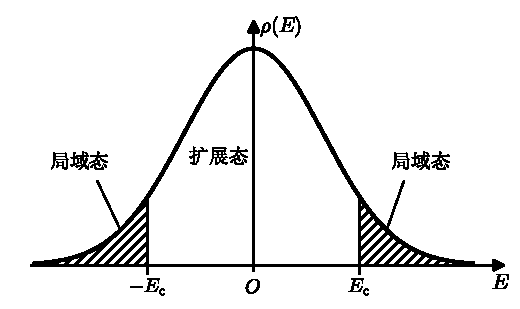
\includegraphics[width=7cm]{fig12-4.pdf}\\{\small 图 12.4\quad $\delta<\delta_{\mathrm{c}}$ 时的电子态密度}
\end{minipage}
\end{center}

利用席曼结果式(12.5.38)，很容易证实莫特的上述设想.因为 $\phi\left(E\right)\equiv\langle\ln|Vg|\rangle$ 与E的关系已求出，将它代入自能 $\Sigma\left(l;E\right)$ 的收敛条件式(12.5.37)，就可以求得任意E态的定域化条件为
\begin{equation}
  \delta=\frac{W}{2Z|V|}>\delta_{\mathrm{c}}\left(E\right)
  \equiv\frac{e}{\left|1-\left(\frac{2E}{W}\right)^{2}\right|^{1/2}}
  \left|\frac{1-\frac{2E}{W}}{1+\frac{2E}{W}}\right|^{\frac{E}{W}}
\end{equation}
对于给定 $\delta$（即W与 $|V|$）的无序系统，当 $\delta$ 略小于 $\mathrm{e}\equiv\delta_{\mathrm{c}}\left(0\right)$ 时，在紧束缚近似能带范围 $\left(|E|\leqslant Z|V|\right)$ 内的状态限于 $\dfrac{2|E|}{W}<\dfrac{1}{\mathrm{e}}$，这时 $\delta_{\mathrm{c}}\left(E\right)$ 将随 $|E|$ 增大而减少，因此 $|E|$ 超过某能量界 $|E_{\mathrm{c}}|$ 的电子态能够满足定域化条件式(12.5.41)，说明无序将使紧束缚近似能带的部分扩展态变为定域态，局域态靠近带边，扩展态在带中心附近.此外，对于无序系统当然还应存在 $|E|>Z|V|$ 的本征态，它与带边相接形成带尾，带尾中状态也是定域态.莫特在此基础上指出，对于非晶态半导体，由于势场的无规起伏还没有达到临界值 $\delta_{\mathrm{c}}\left(0\right)$，因而在非晶半导体中同时存在电子的定域态和扩展态，也存在它们之间的明显分界 $E_{\mathrm{c}}$——迁移率边界，这就是非晶态半导体的莫特模型.

莫特还进一步提出了安德逊转变（Anderson transition）\textsuperscript{[12]}的概念，如果在Si晶体中掺入施主杂质磷（P，5价），由于施主杂质的分布是无规的，就形成无序系统，无序性将导致有一个迁移率边缘，设导带中电子的费密能 $E_{\mathrm{F}}$ 位于迁移率边缘之下（从导带底看），此时系统中电子态都是定域态，可认为是一个“绝缘体”.如果继续掺杂，使费密能级通过迁移率边缘，位于它的上面，系统将表现出“金属性”，因为在扩展态上占有电子.这里发生了从绝缘体向金属的转变，称为安德逊转变.安德逊转变来源于无序效应，它与第十一章§1中所介绍的莫特转变不同，莫特转变是电子间关联作用导致的金属-绝缘体转变.

应当指出，莫特模型仍然存在着争议，争论的焦点在于是否存在迁移率边界.根据莫特的观点，随着无序度 $\delta$ 增大，系统的电导率将减小，在临界值 $\delta_{\mathrm{c}}$ 处电导率有一个跳跃，从有限值变为零，在这里存在着扩展态的最小电导率 $\sigma_{\mathrm{min}}$.目前，关于是否有 $\sigma_{\mathrm{min}}$ 的问题在实验和理论上都还存在分歧，是一个尚未争论清楚的问题\textsuperscript{[13]}.

近年来，人们把无序系统的定域态与扩展态类比的看成为两相，借助于处理相变和临界现象的强有力工具，发展了安德逊定域化的标度理论\textsuperscript{[14]}.标度理论证明了：在一维无序系统中，任何小的无序都会导致局域化.在二维情况下理论也肯定了定域态，至于是否存在扩展态尚有争议.至于三维情况，一般都认为有定域态，有扩展态，也有临界的 $\delta_{\mathrm{c}}$ 值.标度理论所求得的 $\delta_{\mathrm{c}}$ 值大致为1，比安德逊和席曼的估计值小2至3倍，看来是比较合理的结果\textsuperscript{[15]}.关于定域化的标度理论将在本章§8中介绍.

\section{定程与变程跳跃电导}

根据上节的讨论，当费密能级 $E_{\mathrm{F}}$ 位于迁移率边界 $E_{\mathrm{c}}$ 之下 $\left(E_{\mathrm{F}}<E_{\mathrm{c}}\right)$ 时，系统中所有的电子均处于定域态，这些定域态的能量无规地分布在相当宽的能量范围内，相邻的定域中心之间往往有较大的能量差，只有在更远的距离才可能找到能量相近的定域中心，如图12.5所示.对于这样一个全由定域态组成的系统，其零温电导率 $\sigma=0$，属于绝缘体.在有限温度T时，电子才可以通过热激活吸收声子的能量，从一个定域中心隧穿到另一个定域中心，产生跳跃电导.换句话说，跳跃（hopping）是指电子从一个定域态到另一个定域态借助声子进行的量子力学隧穿过程\textsuperscript{[16]}.跳跃电导包括两种传导过程：其一是电子的跃迁主要发生在最近邻的定域中心之间，称为定程跳跃电导.其二是电子的转移发生在相距更远、能量差别较小的两个定域中心之间.莫特（Mott）\textsuperscript{[17]}首先研究了这种新的跳跃传导过程，并求出了其最可几的跳迁距离是随温度T变化的，被称为莫特变程跳跃电导.

\begin{center}
\begin{minipage}{7.5cm}
\centering
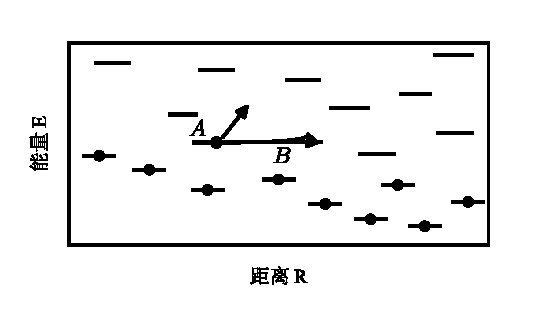
\includegraphics[width=7.5cm]{fig12-5.pdf}\\{\small 图 12.5\quad 定域态间的跳跃传导示意图}
\end{minipage}
\end{center}

现在讨论位于 $\boldsymbol{R}_{i}$ 和 $\boldsymbol{R}_{j}$，能量分别为 $E_{i}$ 和 $E_{j}\ \left(E_{j}>E_{i}\right)$ 的两个定域态之间的电子跃迁.根据量子力学，电子从 $\boldsymbol{R}_{i}$ 中心，经过距离 $R=|\boldsymbol{R}_{i}-\boldsymbol{R}_{j}|$ 隧穿到 $\boldsymbol{R}_{j}$ 中心的概率正比于i与j定域态间波函数的交迭积分之平方.对于定域态，$\phi\left(\boldsymbol{r}-\boldsymbol{R}_{i}\right)\propto\exp\left(-|\boldsymbol{r}-\boldsymbol{R}_{i}|/\lambda\right)$，其中 $\lambda$ 为局域化长度.当两定域态的局域化长度近似相同时，交换积分可表示为
\begin{equation}
  \int\psi^{*}\left(\boldsymbol{r}-\boldsymbol{R}_{i}\right)\psi\left(\boldsymbol{r}-\boldsymbol{R}_{j}\right)\mathrm{d}^{3}r
  \propto\exp\left(-R/\lambda\right)
\end{equation}
因此，$\boldsymbol{R}_{i}$ 与 $\boldsymbol{R}_{j}$ 定域态间的隧穿概率正比于 $\exp\left(-2\alpha R\right)$，其中 $\alpha^{-1}\equiv\lambda$.另一方面，由于两定域态的能量不相同，从 $\boldsymbol{R}_{i}$ 跃迁到 $\boldsymbol{R}_{j}$ 所需的能 $W=E_{j}-E_{i}\ \left(>0\right)$ 必须由热声子供给.因此，在 $T=0$ K时，尽管相邻的定域态之间波函数有明显的重叠，但由于没有热声子的供给，电子无法克服两个定域态之间的能量差W，其实际的跃迁概率仍为零.这就是当 $T=0$ K时定域态系统的电子导率为零的物理原因.仅当温度为有限时，由于具有W能量的热声子数为 $\left[\exp\left(W/k_{\mathrm{B}}T\right)-1\right]^{-1}$，它在 $k_{\mathrm{B}}T\ll W$ 时可用玻耳兹曼因子 $\exp\left(-W/k_{\mathrm{B}}T\right)$ 表示，这时借助于声子供给能量才可能发生跳跃电导.因此，从 $\boldsymbol{R}_{i}$ 到 $\boldsymbol{R}_{j}$ 的跳跃概率不仅正比于隧穿概率 $\exp\left(-2\alpha R\right)$，还应当正比于辅助这一跳跃传导的热平衡声子数 $\exp\left(-W/k_{\mathrm{B}}T\right)$，并写成
\begin{equation}
  w_{ij}=w_{0}\exp\left(-2\alpha R-\frac{W}{k_{\mathrm{B}}T}\right),
  \qquad W=E_{j}-E_{i}>0
\end{equation}
这是讨论定程和变程跳跃电导的基本公式，上式中 $w_{ij}$ 代表电子从已占据态i向空态j转移的每秒跳跃概率，如图12.5中箭头所示.可令 $w_{ij}=\tau_{R}^{-1}$，其中 $\tau_{R}$ 代表电子作步长为R的无规行走所需的时间，$\tau_{R}$ 与 $R^{2}$ 的关系由扩散系数D决定
\begin{equation}
  D=R^{2}/\tau_{R}
\end{equation}
再根据固体物理学中熟知的爱因斯坦关系写出电导率
\begin{equation}
  \sigma=e^{2}DN\left(E_{\mathrm{F}}\right)
\end{equation}
其中 $N\left(E_{\mathrm{F}}\right)$ 为单位体积中的电子态密度，这时利用 $w_{ij}=\tau_{R}^{-1}$ 可求出
\begin{equation}
  \sigma\left(T\right)=\sigma_{0}\exp\left(-2\alpha R-W/k_{\mathrm{B}}T\right)
\end{equation}
其中
\begin{equation}
  \sigma_{0}\equiv w_{0}e^{2}R^{2}N\left(E_{\mathrm{F}}\right)
\end{equation}

\subsection*{1. 定程跳跃电导}

定程跳跃传导发生在最近邻的定域中心之间，这时 $R=R_{0}$，代表最近邻定域中心的平均间距，设无序体系的杂质浓度为 $n_{\mathrm{I}}$，根据 $\left(4\pi/3\right)R_{0}^{3}n_{\mathrm{I}}=1$ 的平均间距条件，求得
\begin{equation}
  R_{0}=\left(\frac{3}{4\pi n_{\mathrm{I}}}\right)^{\frac{1}{3}}
\end{equation}
为一个确定的数值.另一方面，从图12.5可看出：电子跃迁到最近邻中心所需的能量 $W_{0}$ 高于向距离更远的定域中心跃迁所需的能量W（即当 $R>R_{0}$ 时，$W<W_{0}$）.因此，定程跳跃往往出现在有足够多的能量为 $W_{0}$ 的声子可供给近邻跃迁的高温情形.这时式(12.6.5)中 $\exp\left(-2\alpha R_{0}\right)$ 为一常数，特别是在 $\alpha R_{0}\leqslant1$ 的弱定域化情形时 $\exp\left(-2\alpha R_{0}\right)$ 是数量级为一的常数而可以略去，真正随温度变化的因子仅仅来自 $\exp\left(-W_{0}/k_{\mathrm{B}}T\right)$，这时电导率可写为下列热激活形式：
\begin{equation}
  \sigma\left(T\right)=\sigma_{0}\exp\left(-W_{0}/k_{\mathrm{B}}T\right)
\end{equation}
称为定程跳跃电导率.

\subsection*{2. 变程跳跃电导}

莫特\textsuperscript{[17]}首先指出，当温度足够低，热激活声子的数量和能量都很小时，这里几乎没有 $W_{0}$ 能量的声子可辅助最近邻跃迁.但是，电子仍然可以吸收低能量的声子，隧穿到相距较远 $\left(R>R_{0}\right)$ 而能量差又较小 $\left(W<W_{0}\right)$ 的定域态中.当R较大时W与距离R的关系可以从态密度 $N\left(E\right)$ 求得，因为 $N\left(E\right)$ 代表在能量E附近单位体积和单位能量间隔中的状态数.若取定域态 $\boldsymbol{R}_{i}$ 为中心，在半径为R的球体内，能量在E到 $E+\Delta E$ 之间的状态数为 $\left(4\pi/3\right)R^{3}N\left(E\right)\Delta E$，考虑到电导率的主要贡献来自电子在费密能级 $E_{\mathrm{F}}$ 附近的定域态之间的跃迁.因此，在 $\boldsymbol{R}_{i}$ 周围半径为R的球体内找到一个定域态 $E_{j}=E_{i}+W$ 的条件是
\begin{equation}
  \frac{4\pi}{3}R^{3}N\left(E_{\mathrm{F}}\right)W=1
\end{equation}
其中 $W=E_{j}-E_{i}$，$E_{j}>E_{i}$，且都在 $E_{\mathrm{F}}$ 附近很小的能量间隔W之内.由此求出W与R的关系为
\begin{equation}
  W\left(R\right)=\left[\frac{3}{4\pi R^{3}N\left(E_{\mathrm{F}}\right)}\right]
\end{equation}
显然，上式在W较小，也就是R较大时，才能成立.将 $W\left(R\right)$ 代入式(12.6.2)，可以看出从 $\boldsymbol{R}_{i}$ 到 $\boldsymbol{R}_{j}$ 的跃迁概率正比于 $\exp\{-2\alpha R-\left[W\left(R\right)/k_{\mathrm{B}}T\right]\}$，其中两个因子是相互竞争的.当R较大时，尽管波函数的重叠因子 $\exp\left(-2\alpha R\right)$ 下降，但却可从吸收声子的玻耳兹曼因子 $\exp\left[-W\left(R\right)/k_{\mathrm{B}}T\right]$ 中得到更多的补偿，因为W随R增大将迅速减小，导致跃迁率的增加.因此，必须求出同时考虑两个因子时的最可几的跃迁概率，也就是从 $\exp\left[-Q\left(R\right)\right]$ 中的指数项
\begin{equation}
  Q\left(R\right)\equiv 2\alpha R+W\left(R\right)/k_{\mathrm{B}}T
\end{equation}
的极值条件
\begin{equation}
  \frac{\mathrm{d}Q\left(R\right)}{\mathrm{d}R}
  =\frac{\mathrm{d}}{\mathrm{d}R}\left[2\alpha R
  +\frac{3}{4\pi R^{3}N\left(E_{\mathrm{F}}\right)k_{\mathrm{B}}T}\right]=0
\end{equation}
决定.由此求得最可几跳跃步长为
\begin{equation}
  \overline{R}=\left[\frac{9}{8\pi\alpha N\left(E_{\mathrm{F}}\right)k_{\mathrm{B}}T}\right]^{\frac{1}{4}}
\end{equation}
显然，$\overline{R}$ 随温度降低而增大，这种跳跃距离随温度变化的传导过程可称为变程跳跃电导.将 $\overline{R}$ 代入Q后，求得最可几的跃迁概率正比于
\begin{equation}
\begin{aligned}
  \exp\left[-Q\left(\overline{R}\right)\right]
  &=\exp\left[-\frac{8}{3}\alpha\overline{R}\right]\\
  &=\exp\Biggl\{-\frac{8}{3}\alpha
  \left[\frac{9}{8\pi\alpha N\left(E_{\mathrm{F}}\right)k_{\mathrm{B}}T}\right]^{\frac{1}{4}}\Biggr\}\\
  &=\exp\left(-B/T^{\frac{1}{4}}\right)
\end{aligned}
\end{equation}
其中
\begin{equation}
  B\equiv\frac{8}{3}\left(\frac{9}{4\pi}\right)^{\frac{1}{4}}
  \left[\frac{\alpha^{3}}{k_{\mathrm{B}}N\left(E_{\mathrm{F}}\right)}\right]^{\frac{1}{4}}
  \approx2\left[\frac{\alpha^{3}}{k_{\mathrm{B}}N\left(E_{\mathrm{F}}\right)}\right]^{\frac{1}{4}}
\end{equation}
再代入式(12.6.5)，求得变程跳跃的电导率
\begin{equation}
  \sigma\left(T\right)=\sigma_{0}\exp\left[-Q\left(\overline{R}\right)\right]
  =\sigma_{0}\exp\left(-B/T^{\frac{1}{4}}\right)
\end{equation}
上式即是著名的莫特 $T^{\frac{1}{4}}$ 定律，这是三维 $\left(d=3\right)$ 无序系统中变程跳跃电导的特征.对于d维（$d=1,2,3$）系统，经过类似的讨论，不难导出\textsuperscript{[16]}
\begin{equation}
  \sigma\left(T\right)=\sigma_{0}\exp\left(-B/T^{\frac{1}{d+1}}\right)
\end{equation}
其中对于三维 $\left(d=3\right)$ 系统，将再现莫特 $T^{\frac{1}{4}}$ 定律，而对于二维 $\left(d=2\right)$ 和一维 $\left(d=1\right)$ 系统，则得到 $T^{\frac{1}{3}}$ 与 $T^{\frac{1}{2}}$ 规律，这些理论的预言都已得到实验的证实.

从式(12.6.13)可知，变程跳跃的步长 $\overline{R}$ 随温度升高将逐渐减小，这里 $\overline{R}$ 存在一个特征温度 $T_{0}$，它表示当 $\overline{R}=R_{0}$ 时的温度.再根据式(12.6.7)，可得到当跳跃步长减小到最近邻定域态间的平均距离时的一个等式
\begin{equation}
  R_{0}=\left(\frac{3}{4\pi n_{\mathrm{I}}}\right)^{\frac{1}{3}}
  =\left[\frac{9}{8\pi\alpha N\left(E_{\mathrm{F}}\right)k_{\mathrm{B}}T_{0}}\right]^{\frac{1}{4}}
  =\overline{R}
\end{equation}
由此求得特征温度
\begin{equation}
  T_{0}=\frac{1}{k_{\mathrm{B}}}\cdot\frac{9}{8\pi\alpha N\left(E_{\mathrm{F}}\right)}
  \left(\frac{4\pi}{3}n_{\mathrm{I}}\right)^{\frac{4}{3}}
\end{equation}
在高温区，当 $T\geqslant T_{0}$ 时，变程跳跃电导自然地过渡为定程跳跃电导，这时电导率表现为通常的热激活特征 $\sigma\left(T\right)=\sigma_{0}\exp\left(-W_{0}/k_{\mathrm{B}}T\right)$.仅在低温区，当 $T\ll T_{0}$ 时，无序系统中才可能表现出变程跳跃电导的 $\sigma\left(T\right)=\sigma_{0}\exp\left(-B/T^{\frac{1}{4}}\right)$ 特征.

\section{一维无序系统的定域化特征}

历史上莫特和图斯（Twose）\textsuperscript{[18]}首先指出，在一维无序系统中，求解薛定谔方程的结果表明：即使在弱无序势场的影响下，所有的波函数都是指数衰减型的定域态，而不可能存在扩展态解.随后，阿布里科索夫（Abrikosov）等人\textsuperscript{[19]}又利用场论方法作出了相应的微观证明，但是这些理论都比较繁琐，本节的目的是希望对一维无序系统的定域化问题作出比较清楚的物理解释.我们将采用安德逊等人\textsuperscript{[20]}基于兰多尔（Landauer）公式\textsuperscript{[21]}的简单物理论证来说明一维无序系统中电子态的定域化特征.为此，首先介绍描述一维系统电导（conductance）的兰多尔公式.然后，再根据安德逊等人的新方法，从一维无序系统中电阻随样品尺寸变化（即改变标度）的特征，对一维系的定域化问题作出理论解释.

\subsection*{1. 一维兰多尔电导公式}

1970年兰多尔\textsuperscript{[21]}指出，在零温和不计电子间相互作用时，在长度为L的无序系统中，当L比电子的非弹性散射平均距离小得多时，电子只可能受到无规分布杂质的势散射，这是一种保持散射前后能量和动量守恒以及粒子流守恒的弹性散射，而每个杂质的散射都可以看成是电子波在一个势垒上的透射和反射问题.整个一维无序系统相当于一组高度和间距为无规的势垒链，并且在两个杂质的势垒之间电子以平面波方式自由传播，仅当碰到势垒时才发生透射和反射.按此观点讨论一维无序系统中电子传导时，既涉及电子穿透一个散射中心的势垒，还应该考虑电子在相邻杂质的势垒之间的多次反射和透射效应，并且势垒的间距又是完全无规的.因此，当计算一块样品的透射系数T和反射系数R时，还必须对相距不等的诸多两势垒散射作统计平均，这是求解一维无序系统关键点.

兰多尔的主要贡献是假定T和R都已经求得，它既可以代一个杂质散射势垒的T和R，也可以推广用于一段长度为L的无序样品.这时只需将整个无序样品看成一个模拟的势垒，如图12.6(b)所示.当样品两端由理想导体连接并存在电位差 $\Delta V$ 时，系统的电导 $G\equiv\left(I_{\mathrm{t}}/\Delta V\right)$ 可以用透射系数T和反射系数R表示为下列简单形式
\begin{equation}
  G=\left(\frac{e^{2}}{\pi\hbar}\right)\frac{T}{R}
\end{equation}
相应的，通过势垒的电阻为
\begin{equation}
  G^{-1}=\left(\frac{\pi\hbar}{e^{2}}\right)\frac{R}{T}
\end{equation}
习惯上定义 $S\equiv\left(R/T\right)$ 描述势垒的反射与透射比，它实际上代表以 $\left(\pi\hbar/e^{2}\right)$ 为单位的量纲为1的电阻.在以上公式中 $T=|t|^{2}$，$R=|r|^{2}$，t和r分别代表电子的透射和反射概率幅，而T和R又称透射和反射的概率，并且
\begin{equation}
  R+T=1
\end{equation}
满足粒子流守恒条件，如图12.6(b)所示.

\begin{center}
\begin{minipage}{9cm}
\centering
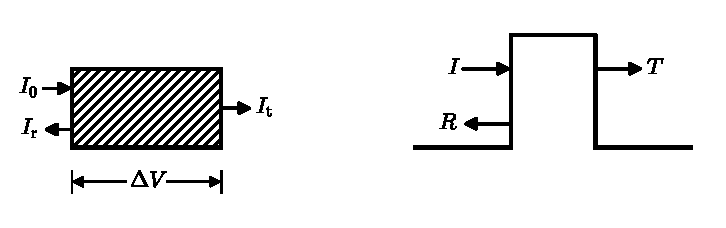
\includegraphics[width=9cm]{fig12-6.pdf}\\[0.3em]
{\small (a) 无序样品的透射与反射电流\qquad\qquad (b) 一维无序样品的模拟势垒}\\[0.2em]
{\small 图 12.6}
\end{minipage}
\end{center}

我们将采用文献[22]所给出的简易方法推导一维系统的兰多尔公式.根据图12.6(a)，设电流 $I_{0}$ 从左侧进入一维样品，而 $I_{\mathrm{r}}=RI_{0}$ 为离开样品左侧的反射电流，在右侧的 $I_{\mathrm{t}}=TI_{0}$ 代表流过一维无序样品的透射电流.由于理想的一维系统其横截面往往小到可以忽略的程度，实际流经样品的电流也将非常小，因此在一维系统中真正有意义的物理量是电流密度j.在固体物理学中，对于d维系统（特别是低于三维的系统）的横截面习惯用 $A_{d}=L^{d-1}$（L为d维超立方体的长度）表示，当 $d=1$ 时即使 $L\rightarrow0$ 也将得到一维横截面 $A_{1}=1$.换句话说，在一维系统中的电流I就是电流密度j，人们往往将一维系统中的j直接称为电流I.因此，我们可以将固体物理学中的 $j=nev_{\mathrm{F}}$ 公式（其中：n是电子浓度，$v_{\mathrm{F}}$ 是费密速度，e是电子电荷）直接用于描述一维系统中的电流I的数值.

考虑到在样品左侧理想导体中的电子浓度 $n_{0}$ 应当包括入射电流 $I_{0}$ 和反射电流 $I_{\mathrm{r}}$ 中的所有电子，并利用入射和反射电流的数值和 $\left(I_{0}+I_{\mathrm{r}}\right)$ 表示为
\begin{equation}
  n_{0}=\frac{\left(I_{0}+I_{\mathrm{r}}\right)}{ev_{\mathrm{F}}}
\end{equation}
在样品右侧的电子浓度 $n_{\mathrm{t}}$ 可根据 $I_{\mathrm{t}}=j_{\mathrm{t}}=n_{\mathrm{t}}ev_{\mathrm{F}}$ 求得
\begin{equation}
  n_{\mathrm{t}}=\frac{I_{\mathrm{t}}}{ev_{\mathrm{F}}}
\end{equation}
因此在无序样品两侧理想导线之间的电子浓度差为
\begin{equation}
  \Delta n=n_{0}-n_{\mathrm{t}}=\frac{\left(I_{0}+I_{\mathrm{r}}-I_{\mathrm{t}}\right)}{ev_{\mathrm{F}}}
  =\frac{2RI_{0}}{ev_{\mathrm{F}}}
\end{equation}
其中R为反射系数，显然浓度差 $\Delta n$ 导致反射电流 $I_{\mathrm{r}}$ 的存在.此外，在上式中还利用了
\begin{equation}
  I_{\mathrm{t}}=TI_{0},\qquad I_{\mathrm{r}}=RI_{0}
\end{equation}
以及粒子流守恒条件 $T+R=1$.正是由于样品两侧存在电位差 $\Delta V$，使电子在两侧的浓度差 $\Delta n$ 保持不变，形成恒定的反射电流 $I_{\mathrm{r}}$.另一方面，确定的 $\Delta V$ 将维持 $I_{0}$ 不变，同时又维持了恒定的透射电流 $I_{\mathrm{t}}=TI_{0}$.$\Delta n$ 与 $\Delta V$ 的关系可以利用样品两侧理想导体中费密面上的电密度 $N\left(E_{\mathrm{F}}\right)$ 求出
\begin{equation}
  \Delta n=2N\left(E_{\mathrm{F}}\right)e\Delta V
\end{equation}
其中因子2来源于自旋简并，$N\left(E_{\mathrm{F}}\right)$ 代表费密能级 $E_{\mathrm{F}}$ 处的电子态密度
\begin{equation}
  N\left(E\right)=\frac{\mathrm{d}n\left(p\right)}{\mathrm{d}E}
  =\left[\frac{\mathrm{d}n\left(p\right)}{\mathrm{d}p}\right]\left(\frac{\mathrm{d}p}{\mathrm{d}E}\right)
\end{equation}
由于 $n\left(p\right)=\left(p/\pi\hbar\right)$ 代表一维系统中在动量p以内的状态数，而 $E\left(p\right)\equiv\left(p^{2}/2m\right)$，以及 $p=mv$，可求出 $\left[\mathrm{d}n\left(p\right)/\mathrm{d}p\right]=\left(1/\pi\hbar\right)$ 和 $\left(\mathrm{d}p/\mathrm{d}E\right)=1/v$.因此
\begin{equation}
  N\left(E_{\mathrm{F}}\right)=\left(1/\pi\hbar v_{\mathrm{F}}\right)
\end{equation}
代入 $\Delta n$ 公式(12.7.8)，求出
\begin{equation}
  \Delta V=\frac{\pi\hbar v_{\mathrm{F}}}{2e}\Delta n
\end{equation}
若再将公式(12.7.6)代入上式右边，可得到 $\Delta V=\left(\pi\hbar/e^{2}\right)RI_{0}$.最后，利用 $I_{\mathrm{t}}=TI_{0}$，即可求出一维无序系统的电导公式(12.7.1)
\begin{equation*}
  G\equiv\frac{I_{\mathrm{t}}}{\Delta V}=\left(\frac{e^{2}}{\pi\hbar}\right)\frac{T}{R}
\end{equation*}
此即著名的一维兰多尔电导公式，它是一个适用于描述弹性散射的普遍公式.由于弹性散射就是势散射，它总可以用一个模拟的势垒以及相应的透射系数T和R来表示传导过程.但应注意，当公式推广用于尺寸为L的一维样品时，必须要求L小于非弹性散射的平均距离.20世纪80年代以来，兰多尔公式已普遍应用无序系统，特别是讨论弱定域化问题.近年来，由于实验技术的发展，人们已能制备样品尺寸小于非弹性散射平均间距的介观器件，给兰多尔公式提供了更广阔的应用天地，并已成为研究介观体系的一个普遍公式.

上述兰多尔公式只考虑了在两端连接导线的单个能带中费密能级附近的电子透射与反射，称为单通道的兰多尔公式.对于高维系统，由于连接导线在垂直方向受到尺寸的限制，将产生横向的能级分裂，使样品两端理想导体中的电子分布在横向能级 $E_{n}\ \left(n=1,2,3,\cdots\right)$ 不相同的子能带之中
\begin{equation}
  E_{n}\left(k\right)=E_{n}+\frac{\hbar^{2}k^{2}}{2m}
\end{equation}
其中每一个 $E_{n}$ 相当于一个一维子能带的带边能.由于相邻 $E_{n}$ 的能级间距随横向尺寸减小而增大，对于理想的一维导体，将因其横向尺寸小到可以忽略的程度而使能级间距（例如 $\Delta E_{12}=E_{2}-E_{1}$）趋向无穷大.这时只需要考虑一个子带中的电子散射，此即一维系统为单通道问题的物理原因.显然，将兰多尔公式推广到二维和三维系统时，必须考虑电子从多个子能带出发对样品中势垒的复杂散射问题，这就是多通道情形.有关多通道的兰多尔公式可参阅文献[23].

\subsection*{2. 一维无序系统的平均电阻计算}

首先考虑含有两个杂质散射中心的系统.当应用兰多尔公式处理这一问题时，可将此系统看作两个势垒，其间由常数势隔开某一距离，如图12.7所示\textsuperscript{[24]}.我们的任务是要求出电子波在双势垒间经多次透射和反射后的透射系数 $T_{12}$ 与两个势垒的透射和反射系数 $\left(T_{1},R_{1}\right)$ 和 $\left(T_{2},R_{2}\right)$ 之间的解析关系.一维无序系统的特征可以看作是由一组具有相同 $\left(T_{1},R_{1}\right)$ 和 $\left(T_{2},R_{2}\right)$，但势垒间距不等的双势垒构成的系综.经正确选择无规变量作系综平均后，才能求得一维无序系统中平均电阻随样品尺寸L的变化关系.

\begin{center}
\begin{minipage}{9cm}
\centering
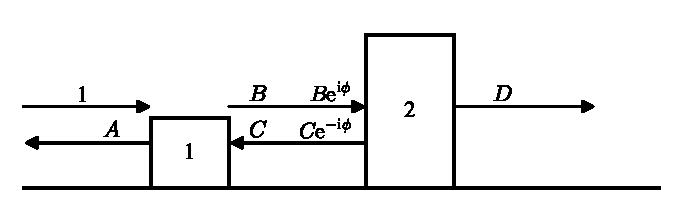
\includegraphics[width=9cm]{fig12-7.pdf}\\{\small 图 12.7\quad 一维无序系统中的双势垒}
\end{minipage}
\end{center}

设入射电子波的振幅为1，经双势垒的多重散射后的总透射与反射波幅分别用D和A表示，而B与C则描述在势垒1右侧的总出射和入射波幅，其中A、B、C和D都是复量.参考图12.7可知，在两势垒之间为常数势场，电子将以平面波 $\mathrm{e}^{\mathrm{i}\left(kx-\omega t\right)}$ 形式自由传播一定距离，必然使1与2两个垫垒内侧的电子之间存在一定的相位差 $\phi$.因此，在图中将势垒2左侧的入射和反射波幅写成 $B\mathrm{e}^{\mathrm{i}\phi}$ 与 $C\mathrm{e}^{-\mathrm{i}\phi}$.现在可以利用 $n=1,2$ 两势垒本身的透射概率幅 $t_{n}$（$T_{n}=|t_{n}|^{2}$——透射系数）和反射概率幅 $r_{n}$ 及反向的反射概率幅 $r_{n}'$（$R_{n}=|r_{n}|^{2}=|r_{n}'|^{2}$——反射系数）写出A、B、C、D所满足的散射方程组
\begin{subequations}
\begin{equation}
  A=r_{1}+Ct_{1}
\end{equation}
\begin{equation}
  B=t_{1}+Cr_{1}'
\end{equation}
\begin{equation}
  C\mathrm{e}^{-\mathrm{i}\phi}=B\mathrm{e}^{\mathrm{i}\phi}r_{2}
\end{equation}
\begin{equation}
  D=B\mathrm{e}^{\mathrm{i}\phi}t_{2}
\end{equation}
\end{subequations}
从上式中(b)、(c)、(d)等方程中消去B和C，求得通过双势垒的透射概率幅 $t_{12}$ 为
\begin{equation}
  t_{12}\equiv D=\frac{\mathrm{e}^{\mathrm{i}\phi}t_{1}t_{2}}
  {1-\mathrm{e}^{\mathrm{i}2\phi}r_{1}'r_{2}}
\end{equation}
因此，双势垒的透射系数
\begin{equation}
  T_{12}=|t_{12}|^{2}=|t_{1}|^{2}
  \frac{1}{|1-\mathrm{e}^{\mathrm{i}2\phi}r_{1}'r_{2}|^{2}}\,|t_{2}|^{2}
\end{equation}
考虑到 $T_{n}=|t_{n}|^{2}$，$r_{1}'=|r_{1}|\mathrm{e}^{-\mathrm{i}\varphi_{1}}=\sqrt{R_{1}}\,\mathrm{e}^{-\mathrm{i}\varphi_{1}}$，$r_{2}=|r_{2}|\mathrm{e}^{\mathrm{i}\varphi_{2}}=\sqrt{R_{2}}\,\mathrm{e}^{\mathrm{i}\varphi_{2}}$，并定义
\begin{equation}
  \theta\equiv 2\phi+\left(\varphi_{2}-\varphi_{1}\right)
\end{equation}
其中 $\phi$ 随1与2势垒的间距变化，这时可将透射系数表示为更简单的形式
\begin{equation}
  T_{12}=\frac{T_{1}T_{2}}{1+R_{1}R_{2}-2\sqrt{R_{1}R_{2}}\cos\theta}
\end{equation}
双势垒的反射系数 $R_{12}$，可利用 $R_{12}+T_{12}=1$ 从 $T_{12}$ 直接求得
\begin{equation}
  R_{12}=\frac{R_{1}+R_{2}-2\sqrt{R_{1}R_{2}}\cos\theta}
  {1+R_{1}R_{2}-2\sqrt{R_{1}R_{2}}\cos\theta}
\end{equation}
最后可将双势垒系统的反射与透射系数比写成
\begin{equation}
  S_{12}=\frac{R_{12}}{T_{12}}
  =\frac{R_{1}+R_{2}-2\sqrt{R_{1}R_{2}}\cos\theta}{T_{1}T_{2}}
  =\frac{1}{T_{12}}-1
\end{equation}
由于在 $\theta$ 因子中还含有两势垒间的相位差 $\phi$，它是一个随势垒间距变化的量，而一维无序系统的主要特征是两个散射中心的间距可随意变化，没有平移对称性.特别是在弱势散射情况，由于杂质的平均间距远大于费密波长，这时 $\phi$ 可取0到 $2\pi$ 间的任一个 $\phi$ 值.对于不同间距的双势垒系统所构成的系综，在0到 $2\pi$ 之间出现任意 $\phi$ 值的概率应当是均等的.因此，我们可以认为 $\theta$ 也以相等的概率出现在0到 $2\pi$ 之间的任意 $\theta$ 角上.安德逊等人正是根据这一特征，计算了函数
\begin{equation}
  f\left(S_{12}\right)=\ln\left(1+S_{12}\right)
  =\ln\left(1+\frac{R_{12}}{T_{12}}\right)=-\ln T_{12}
\end{equation}
的角平均.首先他们计算了 $\ln T_{12}$ 的 $\theta$ 角平均
\begin{equation*}
  \langle\ln T_{12}\rangle=\langle\ln T_{1}\rangle+\langle\ln T_{2}\rangle
  -\left\langle\ln\left(1+R_{1}R_{2}-2\sqrt{R_{1}R_{2}}\cos\theta\right)\right\rangle
\end{equation*}
并令 $a=1+R_{1}R_{2}$ 和 $b=-2\sqrt{R_{1}R_{2}}$，求得上式右边最后一项等于零
\begin{equation}
\begin{aligned}
  \left\langle\ln\left(a+b\cos\theta\right)\right\rangle
  &=\frac{1}{2\pi}\int_{0}^{2\pi}\mathrm{d}\theta\ln\left(a+b\cos\theta\right)\\
  &=\frac{1}{2\pi}\Bigl\{\int_{0}^{\pi}\mathrm{d}\theta\ln\left(a+b\cos\theta\right)\\
  &\qquad-\int_{0}^{\pi}\mathrm{d}\theta\ln\left(a-b\cos\theta\right)\Bigr\}\\
  &=\ln\frac{1}{2}\left[a+\sqrt{a^{2}-b^{2}}\right]
  -\ln\frac{1}{2}\left[a+\sqrt{a^{2}-b^{2}}\right]\\
  &=0
\end{aligned}
\end{equation}
由此求得 $\langle\ln T_{12}\rangle=\langle\ln T_{1}\rangle+\langle\ln T_{2}\rangle$，这是一维无序系统的一个重要特征.若将 $T_{1}$ 与 $T_{2}$ 分别看作是由长度为 $L_{1}$ 和 $L_{2}$ 的两段一维无序样品的透射系数 $T\left(L_{1}\right)$ 和 $T\left(L_{2}\right)$，相应的方程可用反射与透射系数比 $S=R/T$ 表示为
\begin{equation}
  \left\langle\ln\left[1+S\left(L_{1}+L_{2}\right)\right]\right\rangle
  =\left\langle\ln\left[1+S\left(L_{1}\right)\right]\right\rangle
  +\left\langle\ln\left[1+S\left(L_{2}\right)\right]\right\rangle
\end{equation}
这是描述一维无序系统S的对数函数 $f\left(S\right)=\ln\left[1+S\left(L\right)\right]$ 之平均值随样品尺寸改变（即标度变化）的一个重要方程.显然，满足这个方程的解必然是
\begin{equation}
  \langle f\rangle=\left\langle\ln\left[1+S\left(L\right)\right]\right\rangle=\gamma L
\end{equation}
因此，一段长度为L的一维无序样品的 $f=\ln\left[1+S\left(L\right)\right]$ 函数的平均值是L的线性增长函数.安德逊等人还仔细地分析了f函数相对于平均值的均方偏差 $\Delta^{2}\left(L\right)=\langle\left(f-\langle f\rangle\right)^{2}\rangle=\langle f^{2}\rangle-\langle f\rangle^{2}$，并指出在L很大时也具有 $\Delta^{2}\left(L\right)\propto L$ 的线性增长特征\textsuperscript{[20]}.显然，当L很大时f的相对偏差 $\left[\Delta\left(L\right)/\langle f\rangle\right]$ 正比于 $L^{-\frac{1}{2}}$，在 $L\rightarrow\infty$ 时，它趋向于零，满足概率论的中心极限定理（即大数定律），可以用f相对于其平均值 $\langle f\rangle$ 偏离很小的高斯分布描述.因此，作为初级近似，可以认为 $\langle f\rangle$ 就是一维无序系统的实际 $\ln\left[1+S\left(L\right)\right]$ 函数，并求得实际的反射与透射系数比为
\begin{equation}
  S\left(L\right)=\frac{1-T\left(L\right)}{T\left(L\right)}
  =\left(\mathrm{e}^{2\alpha L}-1\right)
\end{equation}
其中设 $\gamma=2\alpha$.由于 $S\left(L\right)$ 实际上代表以 $\left(\pi\hbar/e^{2}\right)$ 为单位的量纲为1的电阻，其倒数定义以 $\left(e^{2}/\pi\hbar\right)$ 为单位的量纲为1的电导，根据式(12.7.1)与式(12.7.24)有
\begin{equation}
  g\left(L\right)\equiv G\left(L\right)/\left(\frac{e^{2}}{\pi\hbar}\right)
  =\frac{T\left(L\right)}{1-T\left(L\right)}
  =\left(\mathrm{e}^{2\alpha L}-1\right)^{-1}
\end{equation}
由此立刻求出一维无序系统的实际透射概率（即透射系数）为
\begin{equation}
  T\left(L\right)=\mathrm{e}^{-2\alpha L}
\end{equation}
因此，在一维无序系统中，经L距离的透射后，电子波的概率幅减小了 $\mathrm{e}^{-\alpha L}$ 倍，从而十分清楚地告诉我们对传导起主要作用的费密能级 $\left(E_{\mathrm{F}}\right)$ 上的电子波函数是指数衰减型 $\exp\left(-|\boldsymbol{r}-\boldsymbol{R}|/\lambda\right)$ 的定域态，其中 $\lambda=\alpha^{-1}$ 代表定域化长度.不言而喻，系统中的其它电子，因其能级 $E<E_{\mathrm{F}}$，也必然处于定域化状态.换句话说，一维无序系统中的所有电子均处于定域化状态.

\subsection*{3. 用量纲为1的电导 $g(L)$ 描述定域化}

由于在“2”中，利用正确的无规平均方法，求得了一维无序系统中量纲为1的电导 $g\left(L\right)$ 随样品长度L变化的公式(12.7.25)，我们可以换一个观点直接从可测物理量 $g\left(L\right)$ 的标度（即L变化）特征来描述一维无序系统的定域化.用标度变化的观点讲：当L增大时，如果量纲为1的电导 $g\left(L\right)$ 随之单调地减小，并在 $L\rightarrow\infty$ 时有 $g\left(L\right)\rightarrow0$ 的特点时，系统处于定域态.反之，当 $g\left(L\right)$ 随L增大单调地上升时，系统处于扩展态.这是一种区分扩展态与定域态的简单而有效的方案，它适用于任意的d维 $\left(d=1,2,3\right)$ 系统.

对于一维无序系统，从式(12.7.25)可以看出，存在 $g\left(L\right)\ll1$ 和 $g\left(L\right)\gg1$ 两个极限
\begin{equation}
  g\left(L\right)=\left(\mathrm{e}^{2L/\lambda}-1\right)^{-1}
  =\begin{cases}
    \dfrac{\lambda}{2L} & \left[g\left(L\right)\gg1\ \text{或}\ L\ll\lambda\right]\\[0.8em]
    \mathrm{e}^{-2L/\lambda} & \left[g\left(L\right)\ll1\ \text{或}\ L\gg\lambda\right]
  \end{cases}
\end{equation}
显然，$g\left(L\right)$ 随着样品尺寸L增大，从 $g\left(L\right)\gg1$ 极限单调地减小，并连续地过渡到另一极限 $g\left(L\right)\ll1$.当 $L\rightarrow\infty$ 时，$g\left(L\right)\rightarrow0$，这说明一维无序系统中电子处于定域态，其中 $g\left(L\right)\gg1$ 极限对应于 $\alpha L\ll1$（$\alpha=\lambda^{-1}$）的弱定域化情形，而另一极限 $\alpha L\gg1$ 则代表强定域化.弱定域化即弱散射情形，后者可用半经典的玻耳兹曼输运理论描述，主要的结论是，对于任意的d维系统，电流密度j与电场强度E之间满足欧姆定律 $j=\sigma E$，其中导电率 $\sigma=\left(ne^{2}l/mv_{\mathrm{F}}\right)$，$v_{\mathrm{F}}$ 为费密速度，l是平均自由程，n代表电子浓度.显然，在弱散射极限，$\sigma$ 是一个与系统尺寸L无关的强度量.用于边长为L的d维立方体，当样品两端存在电位差V时，沿某方向的总电流应为 $I=jL^{d-1}$，其中 $L^{d-1}$ 是垂直流动方向的横截面积.电位差V可认为是L长度样品中均匀电场E所产生，有 $V=EL$ 关系.因此，d维立方体的电导
\begin{equation}
  G\equiv I/V=\left(j/E\right)L^{d-2}
\end{equation}
当欧姆定律 $j=\sigma E$ 成立时，d维系统的电导可表示为
\begin{equation}
  G\left(L\right)=\sigma L^{d-2}
\end{equation}
其中 $\sigma$ 为一个与L无关的常数.对应的量纲为1的电导在弱散射极限为
\begin{equation}
  g\left(L\right)=\left(\frac{\pi\hbar}{e^{2}}\right)\sigma L^{d-2}
\end{equation}
不难看出，满足欧姆定律的电导在 $d=1$ 时正比于 $L^{-1}$，与弱定域化情形（$\alpha L\ll1$ 时）的 $g\left(L\right)=\dfrac{\lambda}{2}L^{-1}$ 相似，比例系数均与L无关.在文献中往往将式(12.7.30)称为扩展态（或金属）极限.以后（见§8）读者将明白，上式仅在 $d>2$ 情形才具有 $g\left(L\right)$ 随L上升而增大的扩展态特征，对于 $d\leqslant2$ 的低维系统（特别是 $d=1$ 时），它仅属于弱定域化情形.但是，$g\left(L\right)\gg1$ 特征却是普遍成立的.因此，确切地说，式(12.7.30)只是d维系统在 $g\left(L\right)\gg1$ 时的渐近表示式.至于另一个极限 $g\left(L\right)\ll1$，若将式(12.7.27)推广到d维系统，可以表示为 $g\left(L\right)=g_{d}\exp\left(-2L/\lambda\right)$，其中 $g_{d}$ 是一个数量级为1，且与L无关的常数.在明白了这些基础知识以后，才能推广讨论在任意维度d时无序系统中定域化的标度理论.历史也正如此，兰多尔早在1970年就导出了描述一维系统定域化的正确公式(12.7.27)，只是他所用的平均方法欠妥当.本节“2”中所介绍的是1980年安德逊等人的改进无规平均方法，但结果仍然与兰多尔一致.

\section{定域化的标度理论}

1979年，亚伯拉罕（E.Abrahams）和安德逊等四人\textsuperscript{[14]}首先提出了无序系统的标度理论.他们采用长度为L的d维块体的量纲为1的电导 $g\left(L\right)$ 作为描述定域化特征的唯一标度参量，并仿照重整化群的标度理论，对不同维度无序体系的定域化特征作出了一系列新的预言，包括：与一维相似，在二维无序体系中也不存在扩展态，所有的态都是定域化的.仅在三维无序体系中，才可能既有定域态又有扩展态，并且从扩展态变为定域态的M-I（金属-绝缘体）转变是连续的，而不存在莫特所预言的最小金属电导率 $\sigma_{\mathrm{min}}$.这些新成果的出现，使人们对安德逊定域化的认识进入了更深的层次，也为无序系统的定域化研究打开了新的窗口.

本节主要介绍描述定域化的标度参量 $g\left(L\right)$，亚伯拉罕等人的标度假定及其对 $d=1,2,3$ 维无序体系的应用.最后指出标度理论所存在的问题.

\subsection*{1. 描述定域化的标度参量 $g(L)$}

在本章§5讨论安德逊无序模型时，已经证明：三维无序系统的特征主要由定域化参数 $\delta\equiv\left(W/2ZV\right)$ 的大小决定，其中Z为近邻格点的配位数，W代表格点（原子）上电子能级的无规分布宽度（即对角无序的量度），而V则描述电子在近邻格点（原子）之间跃迁的交叠能量积分，又称原子间跃迁的共振能量.因此，在原子尺度上看，量纲为1的比值 $\left(V/W\right)$ 正比于定域化参数 $\delta$ 的倒数 $\left(\delta^{-1}\right)$.在标度理论中，人们需要引入一个随系统尺寸L变化的相应量纲为1的参量来描述定域化的标度特征.为此，可将上述讨论作推广，考虑由边长为L的d维立方块体 $\left(L^{d}\right)$ 构成的大样品，设 $V_{L}$ 代表两相邻d维块体间电子跃迁的共振能量，它是原子间跃迁共振能V的块体推广.当 $L\gg l,a$ 时（其中l为电子的平均自由程，a为平均原子间距），还可以引入块体 $L^{d}$ 内电子能级的平均间距 $\Delta_{L}$ 描述无序的强度，因为它正比于电子能级的无规分布的宽度W.$\Delta_{L}$ 可以利用L块体中单位体积内的费密能级态密度 $N_{L}\left(E_{\mathrm{F}}\right)$ 近似决定
\begin{equation}
  \Delta_{L}=\left[N\left(E_{\mathrm{F}}\right)L^{d}\right]^{-1}\sim W
\end{equation}
这是一个随块体尺寸L变化的量.至于近邻块体间的跃迁共振能量 $V_{L}$，当 $L\gg l$ 并略去非弹性散射条件下，可以模拟为电子在近邻块体间的势垒隧穿问题.根据量子力学的不确定关系，$V_{L}=\left(\pi\hbar/\tau_{L}\right)$，可将 $V_{L}$ 改用 $\tau_{L}$ 描述，这里 $\tau_{L}$ 代表电子在近邻块体间通过隧穿转移所需的时间.当两相邻块体间存在电位差 $\widetilde{V}$ 时，将有 $\left[N_{L}\left(E_{\mathrm{F}}\right)L^{d}e\widetilde{V}\right]$ 个状态上的电子从势垒的一侧流向另一侧.相应的，电流可表示为 $I=\left[e^{2}N_{L}\left(E_{\mathrm{F}}\right)L^{d}/\tau_{L}\right]\widetilde{V}$，因此L块体的电导
\begin{equation}
\begin{aligned}
  G\left(L\right)&=e^{2}N_{L}\left(E_{\mathrm{F}}\right)L^{d}/\tau_{L}\\
  &=\frac{e^{2}}{\pi\hbar}\left(V_{L}/\Delta_{L}\right)
\end{aligned}
\end{equation}
其中利用了式(12.8.1)和不确定关系 $V_{L}\tau_{L}=\pi\hbar$.根据上节中讨论，块体的电导 $g\left(L\right)$ 恰好等于块体的量纲为1的比值 $\left(V_{L}/\Delta_{L}\right)$
\begin{equation}
  g\left(L\right)\equiv G\left(L\right)/\left(\frac{e^{2}}{\pi\hbar}\right)=\left(\frac{V_{L}}{\Delta_{L}}\right)
\end{equation}
在文献中 $\left(V_{L}/\Delta_{L}\right)$ 称为索勒斯（Thouless）比，它就是安德逊无序模型中参数 $\delta^{-1}$ 的有限尺寸推广.式(12.8.3)表明：人们可以用可测量的物理量 $g\left(L\right)$ 描述d维块体中定域化特征随标度L的改变，而且是描述无序系统定域化特征的唯一标度参量.因此，当 $L\rightarrow\infty$ 时有 $g\left(L\right)\rightarrow0$，就表示系统处于定域态.反之，当 $L\rightarrow\infty$ 时若 $g\left(L\right)\rightarrow\infty$，则说明系统为扩展态.换句话说，只需要讨论量纲为1的电导 $g\left(L\right)$ 的标度特征，就可以对d维无序系统倒底是处于定域态、扩展态，还是两者兼有等重要问题作出明确的判断.这就是亚伯拉罕等人建立定域化标度理论的思路.

\subsection*{2. 标度假定和标度方程}

亚伯拉罕等人的标度理论是建立在d维电导 $g\left(L\right)$ 在半经典的弱散射极限 $\left[g\left(L\right)\gg1\right]$ 和强定域化极限 $\left[g\left(L\right)\ll1\right]$ 的下列已知特征的一个外插理论.根据式(12.7.30)及其后的讨论，已知
\begin{equation}
  g\left(L\right)=
  \begin{cases}
    \left(\dfrac{\pi\hbar}{e^{2}}\right)\sigma L^{d-2} & \left[g\left(L\right)\gg1\right]\\[0.8em]
    g_{d}\,\mathrm{e}^{-2\alpha L} & \left[g\left(L\right)\ll1\right]
  \end{cases}
\end{equation}
其中 $\sigma$ 为与L无关的常数，$g_{d}$ 是数量级为1的常数.为了进一步讨论 $g\left(L\right)$ 如何随样品尺寸L变化，他们仿照重整化群理论，利用 $\ln g\left(L\right)$ 对 $\ln L$ 的导数描述 $g\left(L\right)$ 的变化，并利用式(12.8.4)写出在上述两种极限情形的已知关系：
\begin{equation}
  \beta=\frac{\mathrm{d}\ln g\left(L\right)}{\mathrm{d}\ln L}
  =\begin{cases}
    d-2 & \left[g\left(L\right)\gg1\right]\\
    \ln\left(g\left(L\right)/g_{d}\right)=-2\alpha L & \left[g\left(L\right)\ll1\right]
  \end{cases}
\end{equation}
其中d表示体系的维度.定域化标度理论是假定在两极限之间对数导数 $\beta$ 随L的变化仅仅通过 $g\left(L\right)$ 的改变表示，即假定 $\beta$ 仅仅是 $g\left(L\right)$ 的函数.$\beta$ 满足下列标度方程：
\begin{equation}
  \beta\left[g\left(L\right)\right]=\frac{\mathrm{d}\ln g\left(L\right)}{\mathrm{d}\ln L}
  =\frac{L}{g\left(L\right)}\,\frac{\mathrm{d}g\left(L\right)}{\mathrm{d}L}
\end{equation}
并且进一步猜测 $\beta$--$\ln g\left(L\right)$ 曲线在两已知极限 $g\left(L\right)\gg1$ 与 $g\left(L\right)\ll1$ 之间连续单调的变化.根据上述假定求解标度方程，可得知 $d=1,2,3$ 维无序体系的标度特征，如图12.8所示.我们将在“3”中对此作进一步的讨论.至于标度方程式(12.8.6)的引入相当于在将样品尺寸扩大b倍时 $\left(L\rightarrow L'=bL\right)$，假定新尺寸的电导 $g\left(bL\right)$ 仅由前一尺寸L时的电导 $g\left(L\right)$ 决定，此即假定
\begin{equation}
  g\left(bL\right)=f\left[g\left(L\right),\,b\right]
\end{equation}

\begin{center}
\begin{minipage}{8cm}
\centering
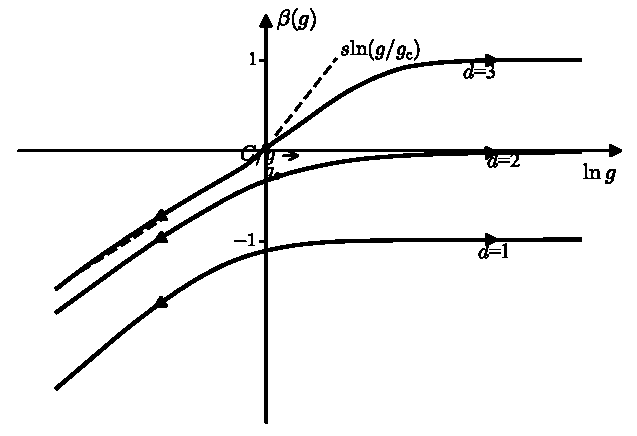
\includegraphics[width=8cm]{fig12-8.pdf}\\{\small 图 12.8\quad $d=1$、2、3 维体系的 $\beta$--$\ln g$ 曲线}
\end{minipage}
\end{center}

这是f是一个与系统具体微观结构无关的普适函数.若令 $b=1+\varepsilon$，其中 $\varepsilon\rightarrow0$，相当于对系统作无限小的标度变换，这时可立刻从上式导出标度方程
\begin{equation}
\begin{aligned}
  \frac{\mathrm{d}\ln g\left(L\right)}{\mathrm{d}\ln\left(L\right)}
  &=\frac{1}{g\left(L\right)}\lim_{\varepsilon\to0}
  \frac{f\left[g\left(L\right),\,1+\varepsilon\right]-f\left[g\left(L\right),\,1\right]}{\varepsilon}\\
  &=\frac{1}{g\left(L\right)}
  \frac{\partial f\left[g\left(L\right),\,b\right]}{\partial b}\bigg|_{b=1}
  \equiv\beta\left[g\left(L\right)\right]
\end{aligned}
\end{equation}
此即式(12.8.6)的标度假定.标度方程的简便之处在于可根据 $\beta$ 取正或负值来判断当标度L改变时电导 $g\left(L\right)$ 是上升或下降，从而区分扩展态与定域态.

\subsection*{3. 标度方程的应用}

现在应用标度方程式(12.8.6)和在两极限的已知 $\beta$ 结果具体讨论一维，三维和二维无序体系的定域化特征.为了简单起见，先讨论 $g\left(L\right)$ 为已知的一维无序系统.

（i）一维系统

这时 $\beta$ 在两个极限均取负值
\begin{equation}
  \beta=
  \begin{cases}
    -1 & \left[g\left(L\right)\gg1,\ g\left(L\right)\sim L^{-1}\right]\\
    -2\alpha L & \left[g\left(L\right)\ll1,\ g\left(L\right)\sim\mathrm{e}^{-2\alpha L}\right]
  \end{cases}
\end{equation}
根据标度假定所作的连续光滑 $\beta$ 曲线如图12.8中 $d=1$ 曲线所示，其中的箭头表示L增大时的流动方向.显然，当L增大时，不仅 $\beta$ 从 $\left(-1\right)$ 降为 $\left(-\infty\right)$，相应的 $g\left(L\right)$ 也单调减小，并在 $L\rightarrow\infty$ 时按指数规律 $\mathrm{e}^{-2\alpha L}$ 趋向于零，说明在一维无序系统中电子处于定域态，而不存在扩展态.由于在上节中我们已经导出了一维无序系统中电导随标度L的变化为 $g\left(L\right)=\left(\mathrm{e}^{2\alpha L}-1\right)^{-1}$，在这里可以直接求出
\begin{equation}
  \beta\left[g\left(L\right)\right]=\frac{\mathrm{d}\ln g\left(L\right)}{\mathrm{d}\ln L}
  =-\left[1+g\left(L\right)\right]\ln\left[1+g^{-1}\left(L\right)\right]
\end{equation}
这就证明了 $\beta$ 的确仅仅是 $g\left(L\right)$ 的函数，并且当L增大时 $g\left(L\right)$ 总是单调的减小，$\beta$ 从 $\left(-1\right)$ 到 $\left(-\infty\right)$ 的流动是单向的，不存在扩展态，这些都与亚伯拉罕等人的标度理论所预言的结果一致.不仅如此，上式还能给出 $\beta\rightarrow\left(-1\right)$ 时 $\beta$ 函数的渐近式
\begin{equation}
  \beta\left[g\left(L\right)\right]=-1-\frac{1}{2g\left(L\right)}
  \qquad\left[g\left(L\right)\gg1\right]
\end{equation}
其中 $-\dfrac{1}{2g\left(L\right)}$ 为，在 $g\left(L\right)\gg1$ 区域内，$\beta$ 函数的修正项.这一结果可推广用于d维系统，并写成
\begin{equation}
  \beta\left[g\left(L\right)\right]=d-2-\frac{C}{g\left(L\right)}
  \qquad\left[g\left(L\right)\gg1\right]
\end{equation}
上式对于 $d=2$、3维情形是一个有用的渐近式，其中常数 $C>0$.

（ii）三维系统

当 $d=3$ 时，式(12.8.5)给出标度函数 $\beta\left(g\right)$ 在两已知极限分别取正、负值
\begin{equation}
  \beta\left(g\right)=
  \begin{cases}
    +1 & \left[g\left(L\right)\gg1,\ g\left(L\right)\sim\sigma L\right]\\
    -2\alpha L & \left[g\left(L\right)\ll1,\ g\left(L\right)\sim\mathrm{e}^{-2\alpha L}\right]
  \end{cases}
\end{equation}
按照标度假定，连接 $\beta=+1$ 与 $\beta=-\infty$（$L\rightarrow\infty$ 时，$\beta\rightarrow-\infty$）两已知极限间的 $\beta\left(g\right)$ 连续曲线必与横轴 $\ln g$ 相交，交点在 $g=g_{\mathrm{c}}$ 处，它是标度函数 $\beta\left(g\right)$ 的零点，满足 $\beta\left(g_{\mathrm{c}}\right)=0$，如图12.8中 $d=3$ 曲线所示.由于 $\beta=0$ 即 $\left(\mathrm{d}g/\mathrm{d}L\right)=0$，因此在 $\beta\left(g_{\mathrm{c}}\right)=0$ 点的电导 $g_{\mathrm{c}}$ 将不随L变化，包括取 $L\rightarrow\infty$ 时该点的电导仍等于 $g_{\mathrm{c}}$，在这个意义上 $g_{\mathrm{c}}$ 被称为不动点.这是一个不稳定的不动点，因为从不动点 $\beta\left(g_{\mathrm{c}}\right)=0$ 的上方 $\left(g>g_{\mathrm{c}}\right)$ 或下方 $\left(g<g_{\mathrm{c}}\right)$ 作标度变换（使L增大）均将导致系统的状态代表点 $g\left(L\right)$ 离开不动点 $g_{\mathrm{c}}$.例如，当 $g>g_{\mathrm{c}}$ 时标度函数 $\beta>0$，由于 $\left(\mathrm{d}g/\mathrm{d}L\right)>0$，$g\left(L\right)$ 必随标度L的增大而升高，表现为状态代表点 $g\left(L\right)$ 将沿 $\beta$ 曲线向上流动，并远离不动点 $g_{\mathrm{c}}$，最后在 $L\rightarrow\infty$ 时到达 $\beta=+1$ 和 $g\rightarrow\infty$ 点，这时系统的 $g\left(L\right)\sim\sigma L$，其中 $\sigma$ 与L无关，称为标准的金属极限.显然，在不动点 $\beta\left(g_{\mathrm{c}}\right)=0$ 的上方 $\beta>0$ 区域内电子具有扩展态特征，被称为三维无序系统的金属（或扩展）区.反之，在不动点的下方从 $g<g_{\mathrm{c}}$ 点出发作标度变换，由于 $\beta<0$，$\left(\mathrm{d}g/\mathrm{d}L\right)<0$，状态代表点 $g\left(L\right)$ 将随L增大而减小，它也将远离不动点但沿 $\beta$ 曲线向下流动，最后到达强定域化极限，并在 $L\rightarrow\infty$ 时按指数规律下降到 $g\rightarrow0$ 和 $\beta\rightarrow-\infty$ 点.因此，在不稳定的不动点下方 $\beta<0$ 区域内，系统具有定域态特征，可称为绝缘（或定域）区.总之，在三维无序系统中既有扩展态，又有定域态，并在不动点 $g_{\mathrm{c}}$ 处发生扩展态与定域态之间的转变，称为金属-绝缘体（M-I）转变.由于 $g>g_{\mathrm{c}}$ 时系统为导体，而 $g<g_{\mathrm{c}}$ 时为绝缘体，不动点 $g_{\mathrm{c}}$ 应与本章§5中的迁移率边界相对应.当无序系统中电子的费密能级 $E_{\mathrm{F}}$ 与迁移率边界的能量 $E_{\mathrm{c}}$ 相等时，到达不动点 $g_{\mathrm{c}}$ 并发生M-I转变.

为了得知在迁移率边界 $E_{\mathrm{c}}$ 附近系统电导率随电子能量E的变化特征，考虑在扩展区靠近不动点 $g_{\mathrm{c}}$ 的一个点 $g_{0}>g_{\mathrm{c}}$，其中 $g_{0}\left(E\right)\equiv g\left(E_{\mathrm{F}},L_{0}\right)$，$L_{0}$ 代表某一微观尺度，而E在 $E_{\mathrm{F}}$ 附近.当 $E_{\mathrm{F}}$ 等于 $E_{\mathrm{c}}$ 时，到达不动点 $g_{\mathrm{c}}=g_{0}\left(E_{\mathrm{c}}\right)\equiv g\left(E_{\mathrm{c}},L_{0}\right)$.对于 $g\left(L\right)$ 十分接近 $g_{\mathrm{c}}$ 情形，根据线性近似，可用标度函数 $\beta$ 在 $g_{\mathrm{c}}$ 点的斜率s表示
\begin{equation}
  \beta\left(g\right)=s\left[g\left(L\right)-g_{\mathrm{c}}\right]
\end{equation}
为了符合金属极限的渐近关系，当 $g\rightarrow\infty$ 时 $\beta\rightarrow1$，人们往往将上式推广为\textsuperscript{[25]}
\begin{equation}
  \beta\left(g\right)=\frac{s\left[g\left(L\right)-g_{\mathrm{c}}\right]}
  {1+s\left[g\left(L\right)-g_{\mathrm{c}}\right]}
\end{equation}
将上式代入标度函数 $\beta$ 的定义式(12.8.6)，并从某一微观尺度 $L_{0}$ $\left[g\left(L_{0}\right)\right.$ 十分接近 $\left.g_{\mathrm{c}}\right]$ 积分到足够大的宏观尺度L（$\beta$ 接近1），可求得下列关系式
\begin{equation}
  \left[\left(\frac{g\left(L_{0}\right)-g_{\mathrm{c}}}{g\left(L\right)-g_{\mathrm{c}}}\right)
  \left(\frac{g\left(L\right)}{g\left(L_{0}\right)}\right)\right]^{\nu}
  \frac{g\left(L_{0}\right)}{g\left(L\right)}=\frac{L_{0}}{L}
\end{equation}
其中 $\nu\equiv\left(sg_{\mathrm{c}}\right)^{-1}$.考虑到在宏观尺度L时 $\beta$ 接近经典的金属极限，等式
\begin{equation}
  \sigma=\left(\frac{e^{2}}{\pi\hbar}\right)\frac{g\left(L\right)}{L}
\end{equation}
成立，并且电导率 $\sigma$ 与L无关，它只是电子能量E（在 $E_{\mathrm{F}}$ 附近）的函数.再考虑到 $g\left(L\right)\gg g_{\mathrm{c}}$ 和 $g\left(L_{0}\right)$ 十分接近 $g_{\mathrm{c}}$，式(12.8.16)可写为
\begin{equation}
  \frac{g\left(L\right)}{L}\approx\frac{g_{\mathrm{c}}}{L_{0}}
  \left(\frac{g_{0}-g_{\mathrm{c}}}{g_{\mathrm{c}}}\right)^{\nu}
\end{equation}
代入式(12.8.17)得到
\begin{equation}
  \sigma\sim\left(g_{0}-g_{\mathrm{c}}\right)^{\nu}
\end{equation}
其中指数 $\nu$ 的数值计算结果大致为1.5.再注意到 $g_{0}\equiv g\left(E,L_{0}\right)$ 和 $g_{\mathrm{c}}\equiv g\left(E_{\mathrm{c}},L_{0}\right)$，当 $g_{0}$ 十分接近不动点 $g_{\mathrm{c}}$ 时，电子能量E必然靠近迁移率边界 $E_{\mathrm{c}}$，有 $\left(g_{0}-g_{\mathrm{c}}\right)\sim\left(E-E_{\mathrm{c}}\right)$ 关系，这时可将电导率表示为
\begin{equation}
  \sigma=\sigma_{\mathrm{c}}\left(E-E_{\mathrm{c}}\right)^{\nu}
\end{equation}
其中 $\sigma_{\mathrm{c}}$ 为一常数.式(12.8.19)与式(12.8.20)表明：改变电子的能量使 $E\rightarrow E_{\mathrm{c}}$ 和 $g_{0}$ 过渡为 $g_{\mathrm{c}}$，三维系统的电导率将连续下降为零，在迁移率边界 $E_{\mathrm{c}}$ 处M-I转变是连续的，不存在莫特所预言的最小金属电导率 $\sigma_{\mathrm{min}}$，这是定域化标度理论的另一个重要结论.

（iii）二维系统

当 $d=2$ 时，应计入弱散射区的修正公式(12.8.12)，并将式(12.8.5)改写为
\begin{equation}
  \beta=
  \begin{cases}
    -C/g\left(L\right) & \left[g\left(L\right)\gg1,\ g\sim\sigma\right]\\
    -2\alpha L & \left[g\left(L\right)\ll1,\ g\sim\mathrm{e}^{-2\alpha L}\right]
  \end{cases}
\end{equation}
上式表明在 $\infty>g\left(L\right)\geqslant0$ 区域内二维系的标度函数 $\beta\left(g\right)$ 总小于零.这时，在 $\beta$ 很小的区域内，对渐近式
\begin{equation*}
  \mathrm{d}\ln g\left(L\right)/\mathrm{d}\ln L=-C/g\left(L\right)
\end{equation*}
作积分，积分的下限取某一微观尺度 $L_{0}$，上限 $L\ll\alpha^{-1}$（其中 $\alpha^{-1}=\lambda$）仍限于弱散射区，得到
\begin{equation*}
  g\left(L\right)=g_{0}-C\ln\left(L/L_{0}\right)
\end{equation*}
其中 $g_{0}$ 为尺度 $L_{0}$ 时的电导.显然，当标度L增大时，状态的代表点从 $g_{0}$ 沿 $d=2$ 曲线向下方流动，与强定域化区内的流向一致，整个二维曲线只有一种向下的流动方向.因此二维体系没有真正的扩展态，它与一维无序体系相似，所有的状态都是定域化的.另一方面，当 $g_{0}$ 很大时，$\beta$ 值接近于零，增大标度时电导的下降十分缓慢，表明在弱定域化区内二维样品仍可能有良好的导电性.

\subsection*{4. 存在的问题}

定域化的标度理论，包括：一维与二维无序体系的基态是绝缘相，只有在三维无序体系中才可能既有绝缘又有金属相，还存在金属-绝缘体转变，并且这个M-I转变是连续的等特征均已得到了实验的支持.近二十年来这些结论已成为一种信念被人们所接受.但是，标度理论只是建立在 $g\gg1$ 和 $g\ll1$ 极限间具有单调外插行为基础上的简单理论，它的主要问题是忽略了电子之间的相互作用.随后的理论研究表明，电子间库仑作用对于一维和三维系统的结论并无本质性的改变，简单标度理论的主要结果仍然适用于一维和三维无序体系.但是对于二维系统，由于它介于一维与三维之间，实际上相当复杂，在理论研究上也一直存在着争议.值得一提的是，早在20世纪80年代中期前苏联学者\textsuperscript{[26]}曾经指出，来自电子间相互作用的量子修正在一定条件下可使二维系统的电阻率随温度降低而减小，从而导致二维系统在低温时可能形成金属相，只是由于当时缺乏实验证据，未能受到重视.近年来由于半导工艺和技术的进步，已经能够在相当宽的范围内调节二维电子系统的浓度.克拉夫钦科（Kravchenko）等人\textsuperscript{[27]}在高质量二维样品中研究了无外磁场时的低温电导特性，他们发现在低浓度下，将实验结果内插到 $T=0$ K时电阻趋向无穷大，表明这时二维系统的基态仍是绝缘性的，与传统的标度理论一致.但是当二维电子系统的浓度超过某临界值后，电阻将随温度降低而减小，并在 $T=0$ K时趋向于零，又表现出金属性，这是与传统的信念相反的新实验结果.换句话说，实验证实了在无外磁场时二维无序体系与三维情形相似，既存在绝缘相又存在金属相，并且改变电子浓度可导致二维系统中出现从绝缘体向金属的转变，这是一个令人吃惊的结果.1997年多布洛舍甫杰维奇（Dobrosavljevic）与亚伯拉罕等人\textsuperscript{[28]}在计入电子间库仑关联的影响后，又提出了一个新的标度理论，其基本点是认为并无任何基本原理要求 $\beta\left(g\right)$ 曲线必须是单调函数以及在 $g\left(L\right)\gg1$ 时二维系统中 $\beta$ 必须为负，因此可以假定在 $g\left(L\right)\gg1$ 时
\begin{equation}
  \beta\left(g\right)=\left(d-2\right)+A/g^{\alpha}+\cdots
  \qquad\left(A>0\right)
\end{equation}
用于代替式(12.8.12)，这时所有的 $d\geqslant2$ 系统 $\beta$ 函数均可能在某些有限的 $g=g_{\mathrm{c}}$ 点上改变符号，导致三维与二维系统中都可能出现M-I转变.对于二维系统可取 $\alpha=1$，其标度行为如图12.9所示.由图可知，在二维无序体系中也可能存在两种基态：其一是具有无限大电阻的绝缘性基态，另一个则是具有无限大电导的金属基态.如何严格证明二维系统的非单调标度行为确实如图12.9所示是当前凝聚态理论研究的一个重要问题.此外，无外磁时二维无序电子系统中是否存在金属基态也还需要更多的实验证据.

\begin{center}
\begin{minipage}{10cm}
\centering
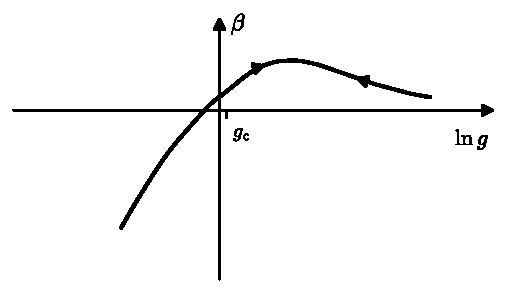
\includegraphics[width=7cm]{fig12-9.pdf}\\{\small 图 12.9\quad 二维系统中 $\beta$--$\ln g$ 曲线的非单调行为}
\end{minipage}
\end{center}

\begin{canKao}
\begin{enumerate}[label={[\arabic*]}, leftmargin=2.2em, itemsep=0pt]
\item Yonezawa F. The Structure and Properties of Matter. Ed. Matsubara T. Berlin: Springer Press, 1982. Chap 11
\item Soven P. Phys Rev, 1967, 156: 809
\item Taylor D W. Phys Rev, 1967, 156: 1017
\item 李正中等. Phys Rev，1994，B50：11332；Phys Rev，1991，B43：12906；Phys Lett，1988，A131：466
\item 许望，李正中. J Phys，1988，C21：4083；J Phys，1990，CM2：109；Solid State Commun，1991，80：943
\item Mott N F. Adv Phys, 1967, 16: 49
\item 李雅达（Lee P W）. 物理通讯，1980，4：46
\item Anderson P W. Phys Rev, 1958, 109: 1492
\item Thouless D J. J Phys, 1970, C3: 1559
\item Ziman J M. J Phys., 1960, C2: 1230; Model of Disorder. Cambridge Univ Press, 1979. Chap 9
\item Licciardello D C, Economon E N. Phys Rev, 1975, B11: 3 697
\item Mott N F et al. Proc Roy Soc (London), 1975, A345: 169
\item 韩汝琦. 自然杂志，1981，3：256
\item Abrahans E, Anderson P W, Licciardello D C, Ramakrisbnan T V. Phys Rev Lett, 1979, 42: 673
\item Sarker S, Domany E. Phys Rev, 1981, B23: 6 018
\item 阎守胜. 固体物理基础. 北京大学出版社，2000
\item Mott N F. J Non Crystal Solids, 1968, 1: 1
\item Mott N F, Twose W D. Adv Phys, 1961, 10: 107
\item Abrikosov A A et al. Adv Phys, 1978, 24: 147
\item Anderson P W et al. Phys Rev, 1980, B22: 3 519
\item Landauer R. Phil Mag, 1970, 21: 863
\item Erdos P et al. Adv Phys, 1982, 31: 65
\item 田光善. 介观物理. 见：阎守胜，甘子钊主编. 北京大学出版社，1995.25
\item Imry Y. Introduction to Mesoscopic Physics. Oxford: Oxford Univ Press, 1997. Chap 5
\item Isihara A. Electron Liqids. New York: Springer, 1992
\item Finkel'stein A M. Z Phys, 1984, B56: 189
\item Kravchenko S V et al. Phys Rev, 1994, 50: 8 039; 1995, 51: 7 038
\item Dobrosavljevic V, Abrahams E et al. Phys Rev Lett, 1997, 42: 673
\end{enumerate}
\end{canKao}


% ---------------- 附录 ----------------
% 附录编号 A–H，公式按 (A.1) 章号编号（原书体例）
\setcounter{chapter}{0}
\renewcommand{\thechapter}{\Alph{chapter}}
\ctexset{chapter={name={附录,}, number={\Alph{chapter}}}}
\counterwithin{equation}{chapter}
\renewcommand{\theequation}{\thechapter.\arabic{equation}}
% ============================================================
%  附录A 推迟格林函数（原书印刷页 533–539）
%  底本：高等教育出版社《固体理论》第二版
%  （PDF 页 = 印刷页 + 20，原书 PDF 页 553–559）
%  公式编号自检：全附录 (A.1)–(A.32) 连续 32 个，无缺号。
%    任务单 tags=31 系 (A.23) 的编号嵌于 OCR 乱码未被计入
%    （原书 p537 在号）；另 (A.12)(A.15)(A.16)(A.21)(A.31) 的
%    OCR tag 残缺（tag{2}/tag{..15}/tag{16}/tag{21}/tag{.31}），
%    均已对照原书页面归位。
%
%  已修正的 OCR/原书错误（除全角句点转"."、删 ~ 间隔符、
%  拆开行内公式与中文等常规项外）：
%  1. 特性 1 小标题 OCR 乱码（"iħℤℋ G_r f{±…}"），按 p533 复原
%     为"1. G_r(t,t')=G_r(t-t')，说明 G_r 代表传播子"。
%  2. 脚注①"可参考祖巴烈夫的总结性文章 Zubarev D N. Soviet
%     Phys. Usp., 1960, 3: 320"OCR 漏失，按 p533 页脚补录。
%  3. (A.4) 各指数因子 OCR 的 h 全部为 ħ 之误识，全附录统一 ħ。
%  4. FM 基态平均式（(A.8) 之下第二例）原书 p534 印
%     "Ŝ_l^+(t)(t)Ŝ_{l'}^-(0)"，(t) 系原书衍字，删一。
%  5. (A.12)(A.15)(A.16) 三块 OCR 乱码按 p535–536 复原；
%     (A.12) 第二行行末 ± 号后接 <0|B|n>…（照原书断行）。
%  6. (A.17) 分式结构按 p536 复原：{exp[β(E_n−E_m)]±1}/
%     {ħω−(E_n−E_m)+iη}。
%  7. (A.18) OCR"e^{βħω_m}"按 p536 复原为 e^{βħω_{nm}}；
%     "\hat{h}ω"、"\hat{⊗}"分别复原为 ħω、δ。
%  8. (A.21) 第三矩阵元 OCR"<m|A|m>"按 p537 复原为 <m|A|n>。
%  9. (A.23) 整块 OCR 乱码按 p537 复原（含右端按上半/下半复平面
%     取 G_r/G_a 的分段表示）。
% 10. (A.26) 分子 [exp(βE'_{nm})±1] 按原书补全（OCR 括号残缺）。
% 11. 原书 p538 (A.29) 印"(e^{βE'_{nm}}∓1)"，按 (A.26) 分子及
%     代回 (A.28) 应恰得 <BA> 判定 ∓ 为 ± 之误，改 ±1。
% 12. (A.30)(A.31) 指数因子 OCR 均作 e^{-βE'_n}±e^{-βE'_n}，按
%     p539 复原为 e^{-βE'_m}±e^{-βE'_n}。
% 13. 原书 p539 末段"我们还将用它建立利用它建立介电函数的严格
%     公式"衍"利用它建立"四字（与上下文重复），删。
% 14. 体例：< <A|B> > 统一 \langle\langle…\rangle\rangle；花体
%     ℋ、ℰ 统一 \mathscr；虚单位 i、指数底 e 及 Tr 用正体。
%  遗留问题：
%  · 无。
% ============================================================
\chapter{推迟格林函数}

在海森伯绘景中任意两个算符 $A$ 与 $B$ 所组成的函数
\begin{equation}
\begin{aligned}
G_{\mathrm{r}}(t,t')&=-\frac{\mathrm{i}}{\hbar}\theta(t-t')
\langle[A(t),B(t')]_{\pm}\rangle\\
&=\left\{
\begin{aligned}
&-\frac{\mathrm{i}}{\hbar}\bigl(\langle A(t)B(t')\rangle
\pm\langle B(t')A(t)\rangle\bigr)\qquad(t>t')\\
&0\qquad(t<t')
\end{aligned}\right.\\
&\equiv\langle\langle A(t);B(t')\rangle\rangle_{\mathrm{r}}\text{，}
\end{aligned}
\end{equation}
称为双时推迟格林函数. $G_{\mathrm{r}}$ 是玻戈留玻夫等人首先引入的\footnote{可参考祖巴烈夫的总结性文章 Zubarev D N. Soviet Phys. Usp., 1960, 3: 320}，$\langle\langle A(t);B(t')\rangle\rangle_{\mathrm{r}}$ 是双时推迟格林函数的玻氏记号，其中泊松括号下角的 $\pm$ 号可根据方便与需要选取. 当 $A$ 和 $B$ 属于费密型算子时，满足反对易律，取 $+$ 号比较方便，而对于玻色型算子，满足对易律，往往取 $-$ 号. 式(A.1)中 $\langle\cdots\rangle$ 代表统计平均，对于正则系综
\begin{equation}
\langle A\rangle=Z^{-1}\mathrm{Tr}(\mathrm{e}^{-\beta H}A)
\text{，}\quad Z=\mathrm{Tr}(\mathrm{e}^{-\beta H})
\text{，}\quad\beta=(k_{\mathrm{B}}T)^{-1}
\end{equation}
$G_{\mathrm{r}}$ 是实时间的温度格林函数，代表海森伯绘景中的一种有用的时间关联函数，有下列重要特性：

\subsection*{1. $G_{\mathrm{r}}(t,t')=G_{\mathrm{r}}(t-t')$，说明 $G_{\mathrm{r}}$ 代表传播子}

由于算符的乘积在 $\mathrm{Tr}$ 号内具有循环性
\begin{equation}
\mathrm{Tr}(ABC)=\mathrm{Tr}(CAB)=\mathrm{Tr}(BCA)
\end{equation}
因此
\begin{equation}
\begin{aligned}
\langle A(t)B(t')\rangle&=Z^{-1}\mathrm{Tr}
\bigl(\mathrm{e}^{-\beta H}\mathrm{e}^{\frac{\mathrm{i}}{\hbar}Ht}
A\mathrm{e}^{-\frac{\mathrm{i}}{\hbar}H(t-t')}
B\mathrm{e}^{-\frac{\mathrm{i}}{\hbar}Ht'}\bigr)\\
&=Z^{-1}\mathrm{Tr}\bigl(\mathrm{e}^{-\beta H}
\mathrm{e}^{\frac{\mathrm{i}}{\hbar}H(t-t')}
A\mathrm{e}^{-\frac{\mathrm{i}}{\hbar}H(t-t')}B\bigr)\\
&=Z^{-1}\mathrm{Tr}\bigl[\mathrm{e}^{-\beta H}A(t-t')B\bigr]\\
&=\langle A(t-t')B(0)\rangle
\end{aligned}
\end{equation}
同理可证明
\begin{equation}
\langle B(t')A(t)\rangle=\langle B(0)A(t-t')\rangle
\end{equation}
于是双时推迟格林函数
\begin{equation}
\begin{aligned}
G_{\mathrm{r}}(t-t')&=-\frac{\mathrm{i}}{\hbar}\theta(t-t')
\langle[A(t),B(t')]_{\pm}\rangle\\
&=-\frac{\mathrm{i}}{\hbar}\theta(t-t')
\langle[A(t-t'),B(0)]_{\pm}\rangle\\
&=G_{\mathrm{r}}(t-t')
\end{aligned}
\end{equation}
说明 $G_{\mathrm{r}}$ 只是时间差 $(t-t')$ 的函数，特性 1 得证. 根据式(A.6)，可以简单的取 $t'=0$，并令 $t$ 代表时间差，则推迟格林函数的定义简化为
\begin{equation}
G_{\mathrm{r}}(t)\equiv\langle\langle A(t);B\rangle\rangle_{\mathrm{r}}
=-\frac{\mathrm{i}}{\hbar}\theta(t)\langle[A(t),B]_{\pm}\rangle
\end{equation}
其中 $B=B(0)$，而
\begin{equation}
A(t)=\mathrm{e}^{\frac{\mathrm{i}}{\hbar}Ht}
A\mathrm{e}^{-\frac{\mathrm{i}}{\hbar}Ht}
\end{equation}
$G_{\mathrm{r}}(t)$ 与实验测量直接有关，是最重要的一种格林函数. 例如，设 $A=\hat{S}_{l}^{+}$ 和 $B=\hat{S}_{l'}^{-}$ 所组成的双时推迟格林函数在 $t>0$ 时为
\begin{equation*}
\begin{aligned}
G_{\mathrm{r}}(t)&=\langle\langle\hat{S}_{l}^{+}(t);
\hat{S}_{l'}^{-}(0)\rangle\rangle_{\mathrm{r}}\\
&=-\frac{\mathrm{i}}{\hbar}\bigl\{\langle\hat{S}_{l}^{+}(t)
\hat{S}_{l'}^{-}(0)\rangle
-\langle\hat{S}_{l'}^{-}(0)\hat{S}_{l}^{+}(t)\rangle\bigr\}
\end{aligned}
\end{equation*}
当 $T=0$ K 时，对于铁磁自旋晶格 $G_{\mathrm{r}}(t)$ 由 FM 相的基态平均表示
\begin{equation*}
\begin{aligned}
G_{\mathrm{r}}(t)&=-\frac{\mathrm{i}}{\hbar}\bigl\{\langle0|
\hat{S}_{l}^{+}(t)\hat{S}_{l'}^{-}(0)|0\rangle
\pm\langle0|\hat{S}_{l'}^{-}(0)\hat{S}_{l}^{+}(t)|0\rangle\bigr\}\\
&=-\frac{\mathrm{i}}{\hbar}\langle0|\hat{S}_{l}^{+}(t)
\hat{S}_{l'}^{-}(0)|0\rangle
\end{aligned}
\end{equation*}
显然，$G_{\mathrm{r}}(t)$ 代表 $t=0$ 时刻在 $l'$ 格点上产生自旋偏离，经过 $t$ 时间在 $l$ 格点所测得的信息. 因此，$\langle\langle\hat{S}_{l}^{+}(t);\hat{S}_{l'}^{-}(0)\rangle\rangle$ 描述晶格中自旋波的传播过程，说明 $G_{\mathrm{r}}(t)$ 是传播子（propagator）.

$G_{\mathrm{r}}(t)$ 的傅里叶变换为
\begin{equation}
G_{\mathrm{r}}(t)=\frac{1}{2\pi}\int_{-\infty}^{\infty}
\mathrm{d}\omega\,G_{\mathrm{r}}(\omega)
\exp[-\mathrm{i}(\omega+\mathrm{i}\eta)t]\qquad(\eta=+0)
\end{equation}
其逆变换
\begin{equation}
G_{\mathrm{r}}(\omega)=\int_{-\infty}^{\infty}
\mathrm{d}t\,G_{\mathrm{r}}(t)\exp[\mathrm{i}(\omega+\mathrm{i}\eta)t]
\end{equation}
在实际运算时，更多的是讨论格林函数 $G_{\mathrm{r}}(\omega)$ 的特性

\subsection*{2. $G_{\mathrm{r}}(\omega)$ 的极点确定互作用系统的元激发}

为简单起见先讨论 $T=0$ K 时 $G_{\mathrm{r}}(\omega)$ 的特性. 设 $|n\rangle$ 与 $E_{n}$ 代表互作用系统哈密顿量 $H$ 的严格本征态和能量本征值，$|0\rangle$ 和 $E_{0}$ 为 $H$ 的基态和基态能. 利用矩阵元关系
\begin{equation}
\langle0|A(t)|n\rangle=\langle0|A|n\rangle
\exp\biggl\{-\frac{\mathrm{i}}{\hbar}(E_{n}-E_{0})\biggr\}
\end{equation}
并考虑到 $T=0$ K 时式(A.7)中只需取基态平均，可求出
\begin{equation}
\begin{aligned}
G_{\mathrm{r}}(t)&=-\frac{\mathrm{i}}{\hbar}\theta(t)
\bigl\{\langle0|A(t)B|0\rangle\pm\langle0|BA(t)|0\rangle\bigr\}\\
&=-\frac{\mathrm{i}}{\hbar}\theta(t)\sum_{n}\bigl\{
\langle0|A|n\rangle\langle n|B|0\rangle
\exp(-\mathrm{i}\omega_{n0}t)\pm\\
&\qquad\langle0|B|n\rangle\langle n|A|0\rangle
\exp(\mathrm{i}\omega_{n0}t)\bigr\}
\end{aligned}
\end{equation}
其中
\begin{equation}
\omega_{n0}\equiv\frac{1}{\hbar}(E_{n}-E_{0})
\end{equation}
根据式(A.10)，对 $G_{\mathrm{r}}(t)$ 的表示式(A.12)作傅里叶变换
\begin{equation}
\begin{aligned}
G_{\mathrm{r}}(\omega)&=\frac{1}{\hbar}\sum_{n}\biggl\{
\frac{\langle0|A|n\rangle\langle n|B|0\rangle}
{\omega-\omega_{n0}+\mathrm{i}\eta}
\pm\frac{\langle0|B|n\rangle\langle n|A|0\rangle}
{\omega+\omega_{n0}+\mathrm{i}\eta}\biggr\}\\
&\equiv\langle\langle A|B\rangle\rangle_{\omega+\mathrm{i}\eta}
\end{aligned}
\end{equation}
上式称为推迟格林函数的莱曼（Lehmann）表示. 从式(A.14)可知，$G_{\mathrm{r}}(\omega)$ 的极点在下半复平面，它在上半复平面是解析函数，玻戈留玻夫采用记号 $\langle\langle A|B\rangle\rangle_{\omega+\mathrm{i}\eta}$ 明确表示 $G_{\mathrm{r}}(\omega)$ 的这一解析性. 由于 $G_{\mathrm{r}}(\omega)$ 极点的实轴坐标为 $\pm\omega_{n0}$，因此只要能求出格林函数 $G_{\mathrm{r}}(\omega)$，就可以由其极点确定 $\omega_{n0}$，从式(A.13)知道，$\hbar\omega_{n0}$ 是互作用系统激发态 $E_{n}$ 与基态 $E_{0}$ 之差，它正好代表系统的元激发能量. 这就证明了，从格林函数 $G_{\mathrm{r}}(\omega)$ 之极点可决定多体系统的元激发谱. 另一方面，从式(4.5.21)可知，$G_{\mathrm{r}}(\omega)$ 是响应随外场振荡的振幅
\begin{equation*}
\Delta A=G_{\mathrm{r}}(\omega)\exp(-\mathrm{i}\omega t+\eta t)
\end{equation*}
当外扰动频率 $\omega$ 与系统的本征频率 $\omega_{n0}$ 相等时，将发生共振，此时振幅 $G_{\mathrm{r}}(\omega)$ 必为无限大. 所以，从物理分析也说明，格林函数 $G_{\mathrm{r}}(\omega)$ 的极点应给出元激发的信息.

对于有限温度，由于各种本征态 $|n\rangle$ 均以概率 $Z^{-1}\mathrm{e}^{-\beta E_{n}}$ 出现，这时式(A.7)中 $\langle(\cdots)\rangle$ 不再是基态平均 $\langle0|(\cdots)|0\rangle$，而应当取统计平均 $Z^{-1}\sum_{n}\mathrm{e}^{-\beta E_{n}}\langle n|(\cdots)|n\rangle$. 按此，将式(A.12)推广到 $T>0$ K 时应写成
\begin{equation}
\begin{aligned}
G_{\mathrm{r}}(t)&=-\frac{\mathrm{i}}{\hbar}\theta(t)Z^{-1}
\sum_{n,m}\mathrm{e}^{-\beta E_{n}}\bigl\{\langle n|A|m\rangle
\langle m|B|n\rangle\mathrm{e}^{\mathrm{i}\omega_{mn}t}\pm\\
&\qquad\langle n|B|m\rangle\langle m|A|n\rangle
\mathrm{e}^{-\mathrm{i}\omega_{mn}t}\bigr\}
\end{aligned}
\end{equation}
其中 $\hbar\omega_{nm}\equiv(E_{n}-E_{m})$. 再对上式右边第一项作变量代换 $n\leftrightarrow m$，立刻得到 $T>0$ K 时的 $G_{\mathrm{r}}(t)$ 为
\begin{equation}
\begin{aligned}
G_{\mathrm{r}}(t)&=-\frac{\mathrm{i}}{\hbar}\theta(t)Z^{-1}
\sum_{n,m}\exp(-\beta E_{n})\langle n|B|m\rangle
\langle m|A|n\rangle\times\\
&\quad\exp\biggl\{-\frac{\mathrm{i}}{\hbar}(E_{n}-E_{m})t\biggr\}
\bigl\{\exp[\beta(E_{n}-E_{m})]\pm1\bigr\}
\end{aligned}
\end{equation}
经傅里叶变换求得 $T>0$ K 时的莱曼表示
\begin{equation}
\begin{aligned}
G_{\mathrm{r}}(\omega)&=Z^{-1}\sum_{n,m}\exp(-\beta E_{n})
\langle n|B|m\rangle\langle m|A|n\rangle\times\\
&\quad\frac{\exp[\beta(E_{n}-E_{m})]\pm1}
{\hbar\omega-(E_{n}-E_{m})+\mathrm{i}\eta}
\equiv\langle\langle A|B\rangle\rangle_{\omega+\mathrm{i}\eta}
\end{aligned}
\end{equation}
若引入谱函数
\begin{equation}
\begin{aligned}
A(\omega)&\equiv-\frac{1}{\pi}\mathrm{Im}G_{\mathrm{r}}(\omega)\\
&=Z^{-1}\sum_{n,m}\mathrm{e}^{-\beta E_{n}}\langle n|B|m\rangle
\langle m|A|n\rangle\bigl(\mathrm{e}^{\beta\hbar\omega_{nm}}\pm1\bigr)
\delta\bigl[\hbar\omega-(E_{n}-E_{m})\bigr]\\
&=Z^{-1}\sum_{n,m}\langle n|B|m\rangle\langle m|A|n\rangle
\bigl(\mathrm{e}^{-\beta E_{m}}\pm\mathrm{e}^{-\beta E_{n}}\bigr)
\delta\bigl[\hbar\omega-(E_{n}-E_{m})\bigr]
\end{aligned}
\end{equation}
还可导出格林函数 $\langle\langle A|B\rangle\rangle_{\omega}$ 与平均量 $\langle BA\rangle$ 的严格关系——谱定理.

\subsection*{3. 谱定理}

根据式(A.18)，容易证明谱函数 $A(\omega)$ 与分布函数的乘积对频率的积分恰好等于平均量 $\langle BA\rangle$.
\begin{equation}
\begin{aligned}
\int_{-\infty}^{\infty}\frac{A(\omega)}
{\mathrm{e}^{\beta\hbar\omega}\pm1}\mathrm{d}\omega
&=Z^{-1}\sum_{n,m}\mathrm{e}^{-\beta E_{n}}\langle n|B|m\rangle
\langle m|A|n\rangle\\
&=Z^{-1}\sum_{n}\mathrm{e}^{-\beta E_{n}}\langle n|BA|n\rangle\\
&=\langle BA\rangle
\end{aligned}
\end{equation}
再计入 $A(\omega)$ 的定义式(A.18)，求得平均量 $\langle BA\rangle$ 与格林函数 $G_{\mathrm{r}}(\omega)$ 的一个重要关系式
\begin{equation}
\langle BA\rangle=\frac{1}{2\pi}\int_{-\infty}^{\infty}
\frac{\bigl\{-2\,\mathrm{Im}G_{\mathrm{r}}(\omega)\bigr\}}
{\mathrm{e}^{\beta\hbar\omega}\pm1}\mathrm{d}\omega
\end{equation}
上式称为格林函数的谱定理. 在文献中谱定理常被称为涨落-耗散定理（FDT），这是因为 $\mathrm{Im}G_{\mathrm{r}}(\omega)$ 与系统的阻尼有关，而 $\langle BA\rangle$ 可作为描述涨落的关联函数.

推迟格林函数 $\langle\langle A|B\rangle\rangle_{\omega+\mathrm{i}\eta}$ 的极点在下半复平面，它只是上半复平面的解析函数，若将式(A.17)中 $\mathrm{i}\eta$ 换成 $-\mathrm{i}\eta$，则定义一个在下半复平面的解析函数
\begin{equation}
\begin{aligned}
\langle\langle A|B\rangle\rangle_{\omega-\mathrm{i}\eta}
&\equiv Z^{-1}\sum_{n,m}\exp(-\beta E_{n})\langle n|B|m\rangle
\langle m|A|n\rangle\times\\
&\quad\frac{\exp[\beta(E_{n}-E_{m})]\pm1}
{\hbar\omega-(E_{n}-E_{m})-\mathrm{i}\eta}=G_{\mathrm{a}}(\omega)
\end{aligned}
\end{equation}
其极点在下半面，再对 $G_{\mathrm{a}}(\omega)$ 作傅里叶变换
\begin{equation}
\begin{aligned}
G_{\mathrm{a}}(t)&=\frac{1}{2\pi}\int_{-\infty}^{\infty}
\mathrm{d}\omega\,G_{\mathrm{a}}(\omega)
\exp[-\mathrm{i}(\omega-\mathrm{i}\eta)t]\qquad(\eta=+0)\\
&=\frac{\mathrm{i}}{\hbar}\theta(-t)\langle[A(t),B]_{\pm}\rangle
\equiv\langle\langle A(t);B\rangle\rangle_{\mathrm{a}}\\
&=\left\{
\begin{aligned}
&0\qquad(t>0)\\
&\frac{\mathrm{i}}{\hbar}\bigl\{\langle A(t)B\rangle
\pm\langle BA(t)\rangle\bigr\}\qquad(t<0)
\end{aligned}\right.
\end{aligned}
\end{equation}
所求出的时间关联函数逆时序传播，代表超前格林函数，因此用 $G_{\mathrm{a}}(t)$ 与 $G_{\mathrm{a}}(\omega)$ 表示.

利用 $G_{\mathrm{r}}(\omega)$ 与 $G_{\mathrm{a}}(\omega)$ 可定义包括上、下半复平面在内的一个全格林函数
\begin{equation}
\begin{aligned}
G(\omega)&\equiv\langle\langle A|B\rangle\rangle_{\omega}\\
&=Z^{-1}\sum_{n,m}\mathrm{e}^{-\beta E_{n}}\langle n|B|m\rangle
\langle m|A|n\rangle
\frac{\mathrm{e}^{\beta(E_{n}-E_{m})}\pm1}
{\hbar\omega-(E_{n}-E_{m})}\\
&=\left\{
\begin{aligned}
&G_{\mathrm{r}}(\omega)\qquad(\text{上半复平面})\\
&G_{\mathrm{a}}(\omega)\qquad(\text{下半复平面})
\end{aligned}\right.
\end{aligned}
\end{equation}
其中 $\omega$ 为复量. 尽管全格林函数 $G(\omega)$ 在上半面由 $G_{\mathrm{r}}(\omega)$ 定义，而下半面由 $G_{\mathrm{a}}(\omega)$ 定义，但在实轴上却无定义. 这是因为当 $\eta\to+0$ 时，$G_{\mathrm{r}}(\omega)$ 与 $G_{\mathrm{a}}(\omega)$ 分别从上、下岸趋向实轴，它们的实部相等，而虚部则异号，导致在实轴上 $G(\omega)$ 无法定义，人们必须沿实轴作割线才能保证 $G(\omega)$ 的解析性. 但是利用此割线两边 $\mathrm{Im}\,G_{\mathrm{r}}(\omega)$ 与 $\mathrm{Im}\,G_{\mathrm{a}}(\omega)$ 异号和 $\mathrm{Re}G_{\mathrm{r}}(\omega)=\mathrm{Re}G_{\mathrm{a}}(\omega)$ 特征，又可得等式
\begin{equation*}
-2\,\mathrm{Im}G_{\mathrm{r}}(\omega)=\mathrm{i}\bigl\{
\langle\langle A|B\rangle\rangle_{\omega+\mathrm{i}\eta}
-\langle\langle A|B\rangle\rangle_{\omega-\mathrm{i}\eta}\bigr\}
\end{equation*}
并将谱定理改写为
\begin{equation}
\langle BA\rangle=\frac{\mathrm{i}}{2\pi}\int_{-\infty}^{\infty}
\frac{\langle\langle A|B\rangle\rangle_{\omega+\mathrm{i}\eta}
-\langle\langle A|B\rangle\rangle_{\omega-\mathrm{i}\eta}}
{\mathrm{e}^{\beta\hbar\omega}\pm1}\mathrm{d}\omega
\end{equation}
式(A.24)与式(A.20)是等效的，前者是祖巴烈夫最早引入谱定理时的表示式，这两个公式都是由格林函数计算平均量的有用工具.

以上讨论的谱定理和谱表示仅限于正则系综，对于互作用系统，往往需要采用巨正则系综作统计平均
\begin{equation}
\langle X\rangle=Z_{\mathrm{G}}^{-1}\mathrm{Tr}
(\mathrm{e}^{-\beta\mathscr{H}}X)\text{，}\quad
Z_{\mathrm{G}}=\mathrm{Tr}(\mathrm{e}^{-\beta\mathscr{H}})
\text{，}\quad\mathscr{H}=H-\mu\hat{N}
\end{equation}
其中 $Z_{\mathrm{G}}$ 是巨配分函数，$\mu$ 为化学势，$\hat{N}$ 代表总粒子数算符，并取 $\hbar=1$ 单位. 类似于上述讨论，不难证明推迟与超前格林函数在巨正则系综内的莱曼表示式为
\begin{equation}
\begin{aligned}
\langle\langle A|B\rangle\rangle_{\omega\pm\mathrm{i}\eta}
&=Z_{\mathrm{G}}^{-1}\sum_{n,m}\exp(-\beta E_{n}')
\langle n|B|m\rangle\\
&\qquad\times\langle m|A|n\rangle
\frac{\bigl[\exp(\beta E_{nm}')\pm1\bigr]}
{\omega-E_{nm}\pm\mathrm{i}\eta}
\end{aligned}
\end{equation}
其中 $\beta=(k_{\mathrm{B}}T)^{-1}$，$E_{nm}=E_{n}-E_{m}$，$E_{n}$ 是 $H$ 的能量本征值，因此 $E_{nm}$ 代表从 $m$ 态到 $n$ 态的激发能，它正好等于格林函数 $\langle\langle A|B\rangle\rangle_{\omega}$ 的极点，并决定系统的元激发. 上式中的 $E_{n}'$ 代表 $H-\mu\hat{N}$ 的本征值，且 $E_{n}'=E_{n}-\mu N_{n}$，$N_{n}$ 为 $n$ 态时系统的总粒子数，因此
\begin{equation}
E_{nm}'\equiv(E_{n}'-E_{m}')=E_{nm}-\mu\delta N_{nm}=E_{nm}-\mu
\end{equation}
其中 $\delta N_{nm}=N_{n}-N_{m}$ 代表从 $m$ 态激发到 $n$ 态系统总粒子数的变化. 在具体的格林函数中往往取 $B$ 为产生算符，例如单电子格林函数 $\langle\langle C_{k\sigma}|C_{k\sigma}^{+}\rangle\rangle_{\omega+\mathrm{i}\eta}$，这时式(A.26)中出现 $\langle n|C_{k\sigma}^{+}|m\rangle$ 矩阵元，它将限定从 $m\to n$ 仅增加一个粒子，$\delta N_{nm}=1$，从而得到式(A.27)的最后一个等式.

利用莱曼表示式(A.26)和式(A.27)，可以立刻导出巨正则系统的格林函数谱定理为
\begin{equation}
\langle BA\rangle=\frac{\mathrm{i}}{2\pi}\int_{-\infty}^{\infty}
\frac{\langle\langle A|B\rangle\rangle_{\omega+\mathrm{i}\eta}
-\langle\langle A|B\rangle\rangle_{\omega-\mathrm{i}\eta}}
{\mathrm{e}^{\beta(\omega-\mu)}\pm1}\mathrm{d}\omega
\end{equation}
因为
\begin{equation}
\begin{aligned}
&\frac{\mathrm{i}}{2\pi}\bigl\{\langle\langle A|B\rangle\rangle_{\omega+\mathrm{i}\eta}
-\langle\langle A|B\rangle\rangle_{\omega-\mathrm{i}\eta}\bigr\}\\
&\quad=Z_{\mathrm{G}}^{-1}\sum_{n,m}\mathrm{e}^{-\beta E_{n}'}
\langle n|B|m\rangle\langle m|A|n\rangle
\bigl(\mathrm{e}^{\beta E_{nm}'}\pm1\bigr)\delta(\omega-E_{nm})
\end{aligned}
\end{equation}
式(A.28)的等号右边等于
\begin{equation*}
\begin{aligned}
&\frac{\mathrm{i}}{2\pi}\int_{-\infty}^{\infty}\mathrm{d}\omega\,
\frac{\bigl\{\langle\langle A|B\rangle\rangle_{\omega+\mathrm{i}\eta}
-\langle\langle A|B\rangle\rangle_{\omega-\mathrm{i}\eta}\bigr\}}
{\mathrm{e}^{\beta(\omega-\mu)}\pm1}\\
&\quad=Z^{-1}\sum_{n,m}\mathrm{e}^{-\beta E_{n}'}
\langle n|B|m\rangle\langle m|A|n\rangle\\
&\quad=Z^{-1}\sum_{n}\mathrm{e}^{-\beta E_{n}'}\langle n|BA|n\rangle\\
&\quad=\langle BA\rangle
\end{aligned}
\end{equation*}
显然，在巨正则系综的谱定理公式中含有化学势 $\mu$，它是否位于能带之中将直接确定系统是金属还是绝缘体.

类似于式(A.18)的讨论，利用式(A.26)中推迟格林函数的虚部可直接写出巨正则系综的谱函数
\begin{equation}
A(\omega)=Z_{\mathrm{G}}^{-1}\sum_{n,m}\langle n|B|m\rangle
\langle m|A|n\rangle\bigl(\mathrm{e}^{-\beta E_{m}'}
\pm\mathrm{e}^{-\beta E_{n}'}\bigr)
\delta(\omega-E_{n}+E_{m})\text{，}
\end{equation}
由此又可导出谱函数的一个求和规则
\begin{equation}
\begin{aligned}
\int_{-\infty}^{\infty}\mathrm{d}\omega\,A(\omega)
&=Z_{\mathrm{G}}^{-1}\sum_{n,m}\langle n|B|m\rangle
\langle m|A|n\rangle\bigl(\mathrm{e}^{-\beta E_{m}'}
\pm\mathrm{e}^{-\beta E_{n}'}\bigr)\\
&=Z_{\mathrm{G}}^{-1}\sum_{n,m}\mathrm{e}^{-\beta E_{n}'}
\bigl(\langle n|A|m\rangle\langle m|B|n\rangle\pm\\
&\qquad\langle n|B|m\rangle\langle m|A|n\rangle\bigr)\\
&=Z_{\mathrm{G}}^{-1}\sum_{n}\mathrm{e}^{-\beta E_{n}'}
\langle n|[A,B]_{\pm}|n\rangle\\
&=\langle[A,B]_{\pm}\rangle
\end{aligned}
\end{equation}
对于 $A=C$ 和 $B=C^{+}$，当 $C^{+}$ 和 $C$ 分别代表单粒子的产生与消灭算符时，利用玻色子（取 $-$ 号）与费密子（取 $+$ 号）的对易关系 $[C,C^{+}]_{\pm}=1$，上述求和规则简化为
\begin{equation}
\int_{-\infty}^{\infty}\mathrm{d}\omega\,A(\omega)=1
\end{equation}
表明谱函数具有某种归一性. 谱函数在互作用电子系统中有重要应用，我们将在附录 D 中作进一步的介绍.

应当提醒读者，本节所建立的莱曼表示是在假定多体系统哈密顿量 $H$（或 $H-\mu\hat{N}$）的严格本征态 $|n\rangle$ 及能量本征值 $E_{n}$（或 $E_{n}'$）为已知的前提下求得的一个严格的格林函数表示式，实际上人们并不知道 $H$ 与 $H-\mu\hat{N}$ 在一般情况下如何严格求解，因此一般不能用莱曼表示具体计算格林函数，它的主要用处在于证明定理和导出严格关系. 例如，在本节中用于证明谱定理及谱函数的求和规则. 在附录 B 中，我们还将用它建立介电函数的严格公式，用于讨论金属的基态能. 至于具体计算多体系统的格林函数，还需在复平面上建立双时格林函数 $\langle\langle A|B\rangle\rangle_{\omega}$ 的运动方程，并求其近似解. 我们将在附录 C 中介绍格林函数运动方程，而在第十一章中作具体的近似计算.

% ============================================================
%  附录B 介电函数的一般理论（原书印刷页 540–542）
%  底本：高等教育出版社《固体理论》第二版
%  （PDF 页 = 印刷页 + 20，原书 PDF 页 560–562）
%  公式编号自检：全附录 (B.1)–(B.15) 连续 15 个，无缺号，
%    与任务单 tags=15 一致。
%
%  已修正的 OCR/原书错误（除全角句点转"."、删 ~ 间隔符、
%  拆开行内公式与中文等常规项外）：
%  1. 章首"推迟格林函数 <<ρ_q|ρ_q^+>>_c ，"OCR 下标乱码，按
%     p540 复原为 <<ρ_q|ρ_q^+>>_ω。
%  2. (B.1) 整块 OCR 乱码按 p540 复原：1/ε(q,ω)=1−(4πe²/ħq²)
%     Σ_n|<n|ρ_q|0>|²(1/(ω+ω_{n0}+iη)−1/(ω−ω_{n0}+iη))；
%     其中 ω_{n0}=(1/ħ)(ℰ_n−ℰ_0)，花体 ℰ 统一 \mathscr。
%  3. 试探电荷密度式 OCR"−e£_q exp(…)"按 p540 复原为
%     −eξ_q exp(iq·r−iωt+ηt)（η=+0）。
%  4. (B.2) OCR"v(q)Σ_q ρ_q^+"按 p540 复原为 v(q)ξ_q ρ_q^+
%     （ξ_q 在哈密顿量中作常数因子，与 (B.3) 一致）。
%  5. (B.5) 与 (B.10)(B.7)(B.9)(B.12)(B.13)(B.15) 等 OCR 残缺
%     按 p540–542 复原；(B.5) 之首行 G_r(t)=−(i/ħ)θ(t)<[A(t),
%     B(0)]> 原书跨页印于 p540 页末，已并入本式编号块。
%  6. 原书 p541 (B.9) 为两行一块仅一号（∇·D 与 ∇·E），照排
%     （∇·E=4π×(试探电荷密度+感应电荷密度)）。
%  7. (B.9) 上下文"外扰动电荷密度"OCR 乱码按 p541 复原为
%     "试探电荷密度"。
%  8. 体例：< <A|B> > 统一 \langle\langle…\rangle\rangle；
%     虚单位 i、指数底 e 用正体；函数宗量 q 用粗体（照原书）。
%  遗留问题：
%  · 无。
% ============================================================
\chapter{介电函数的一般理论}

利用 $T=0$ K 时推迟格林函数 $\langle\langle\rho_{q}|\rho_{q}^{+}\rangle\rangle_{\omega}$ 的莱曼表示，可以证明电子体系介电函数的严格公式为
\begin{equation}
\begin{aligned}
\frac{1}{\varepsilon(\boldsymbol{q},\omega)}
&=1-\frac{4\pi e^{2}}{\hbar q^{2}}\sum_{n}
|\langle n|\rho_{q}|0\rangle|^{2}\times\\
&\quad\biggl(\frac{1}{\omega+\omega_{n0}+\mathrm{i}\eta}
-\frac{1}{\omega-\omega_{n0}+\mathrm{i}\eta}\biggr)
\end{aligned}
\end{equation}
其中 $\omega_{n0}=\dfrac{1}{\hbar}(\mathscr{E}_{n}-\mathscr{E}_{0})$，$|n\rangle$ 与 $\mathscr{E}_{n}$ 为 $H$ 的严格本征函数和能量本征值，$|0\rangle$ 为严格基态.

［证明］在互作用电子系统中人为的引入试探电荷作为外扰动，设试探电荷密度为
\begin{equation*}
-e\xi_{q}\exp(\mathrm{i}\boldsymbol{q}\cdot\boldsymbol{r}
-\mathrm{i}\omega t+\eta t)\qquad(\eta=+0)
\end{equation*}
$\xi_{q}$ 为一常数，则外扰动场的哈密顿量
\begin{equation*}
H_{\mathrm{e}}(t)=\sum_{j}\int\mathrm{d}\boldsymbol{r}\,
\frac{e^{2}\xi_{q}}{|\boldsymbol{r}_{j}-\boldsymbol{r}|}
\exp(\mathrm{i}\boldsymbol{q}\cdot\boldsymbol{r}
-\mathrm{i}\omega t+\eta t)
\end{equation*}
$\boldsymbol{r}_{j}$ 为电子坐标. 将 $e^{2}/|\boldsymbol{r}_{j}-\boldsymbol{r}|$ 作傅里叶展开，可得
\begin{equation}
\begin{aligned}
H_{\mathrm{e}}(t)&=\frac{4\pi e^{2}}{q^{2}}\xi_{q}\sum_{j}
\mathrm{e}^{\mathrm{i}\boldsymbol{q}\cdot\boldsymbol{r}_{j}}
\mathrm{e}^{-\mathrm{i}\omega t+\eta t}\\
&=v(q)\xi_{q}\rho_{q}^{+}\mathrm{e}^{-\mathrm{i}\omega t+\eta t}
\end{aligned}
\end{equation}
根据式(4.5.14)，外扰动的算符 $B$ 可取作
\begin{equation}
B=v(q)\xi_{q}\rho_{q}^{+}
\end{equation}
利用式(4.5.21)，外扰动所引起电子系统力学量 $A$ 的变化在线性响应范围为
\begin{equation*}
\langle A\rangle_{t}-\langle A\rangle_{t=-\infty}
=G_{\mathrm{r}}(\omega)\exp(-\mathrm{i}\omega t+\eta t)
\end{equation*}
若取 $A=\rho_{q}$，由于无外扰动时 $\rho_{q}$ 的统计平均值为零
\begin{equation*}
\langle\rho_{q}\rangle_{t=-\infty}=0
\end{equation*}
因此，系统密度起伏的 $q$ 分量为
\begin{equation}
\langle\rho_{q}\rangle_{t}=G_{\mathrm{r}}(\omega)
\exp(-\mathrm{i}\omega t+\eta t)
\end{equation}
其中 $G_{\mathrm{r}}(\omega)$ 是 $A=\rho_{q}$ 与 $B=\xi_{q}v(q)\rho_{q}^{+}$ 组成的推迟格林函数
\begin{equation}
\begin{aligned}
G_{\mathrm{r}}(t)&=-\frac{\mathrm{i}}{\hbar}\theta(t)
\langle[A(t),B(0)]\rangle\\
&=\xi_{q}v(q)\biggl\{-\frac{\mathrm{i}}{\hbar}\theta(t)
\langle[\rho_{q}(t),\rho_{q}^{+}]\rangle\biggr\}\\
&=\xi_{q}v(q)\langle\langle\rho_{q}(t);\rho_{q}^{+}\rangle\rangle
\end{aligned}
\end{equation}
其傅里叶变换为
\begin{equation}
G_{\mathrm{r}}(\omega)=\xi_{q}v(q)
\langle\langle\rho_{q}|\rho_{q}^{+}\rangle\rangle_{\omega+\mathrm{i}\eta}
\end{equation}
再利用莱曼表示式(A.14)
\begin{equation}
\begin{aligned}
\langle\langle\rho_{q}|\rho_{q}^{+}\rangle\rangle_{\omega+\mathrm{i}\eta}
&=\frac{1}{\hbar}\sum_{n}\biggl\{
\frac{\langle0|\rho_{q}|n\rangle\langle n|\rho_{q}^{+}|0\rangle}
{\omega-\omega_{n0}+\mathrm{i}\eta}-\\
&\qquad\frac{\langle0|\rho_{q}^{+}|n\rangle\langle n|\rho_{q}|0\rangle}
{\omega+\omega_{n0}+\mathrm{i}\eta}\biggr\}\\
&=\frac{1}{\hbar}\sum_{n}|\langle n|\rho_{q}|0\rangle|^{2}
\biggl(\frac{1}{\omega-\omega_{n0}+\mathrm{i}\eta}-\\
&\qquad\frac{1}{\omega+\omega_{n0}+\mathrm{i}\eta}\biggr)
\end{aligned}
\end{equation}
在后一等式中，利用了各向同性系统的对称关系
$|\langle n|\rho_{-q}|0\rangle|^{2}=|\langle n|\rho_{q}|0\rangle|^{2}$，于是
\begin{equation*}
\langle\rho_{q}\rangle_{t}=\xi_{q}v(q)
\langle\langle\rho_{q}|\rho_{q}^{+}\rangle\rangle_{\omega+\mathrm{i}\eta}
\exp(-\mathrm{i}\omega t+\eta t)
\end{equation*}
因此，外加试探电荷所引起的感应电荷密度为
\begin{equation}
-e\langle\rho_{q}\rangle_{t}\mathrm{e}^{\mathrm{i}\boldsymbol{q}
\cdot\boldsymbol{r}}=-e\xi_{q}v(q)
\langle\langle\rho_{q}|\rho_{q}^{+}\rangle\rangle_{\omega+\mathrm{i}\eta}
\exp(\mathrm{i}\boldsymbol{q}\cdot\boldsymbol{r}
-\mathrm{i}\omega t+\eta t)
\end{equation}
根据电动力学，电位移矢量 $\boldsymbol{D}$ 和电场 $\boldsymbol{E}$ 分别满足
\begin{align}
\nabla\cdot\boldsymbol{D}&=4\pi\times(\text{试探电荷密度})\nonumber\\
\nabla\cdot\boldsymbol{E}&=4\pi\times(\text{试探电荷密度}
+\text{感应电荷密度})
\end{align}
由于扰动和响应都按 $\exp(\mathrm{i}\boldsymbol{q}\cdot\boldsymbol{r}-\omega t+\eta t)$ 型式变化，因此 $\boldsymbol{D}(\boldsymbol{r},t)$ 与 $\boldsymbol{E}(\boldsymbol{r},t)$ 取下列形式
\begin{equation}
\begin{aligned}
\boldsymbol{D}(\boldsymbol{r},t)&=\boldsymbol{D}(\boldsymbol{q},\omega)
\exp(\mathrm{i}\boldsymbol{q}\cdot\boldsymbol{r}-\omega t+\eta t)\\
\boldsymbol{E}(\boldsymbol{r},t)&=\boldsymbol{E}(\boldsymbol{q},\omega)
\exp(\mathrm{i}\boldsymbol{q}\cdot\boldsymbol{r}-\omega t+\eta t)
\end{aligned}
\end{equation}
代入式(B.9)，求得 $\boldsymbol{D}$ 和 $\boldsymbol{E}$ 沿 $\boldsymbol{q}$ 方向的分量（纵向分量）满足方程
\begin{equation}
\mathrm{i}qD(q,\omega)=-4\pi e\xi_{q}
\end{equation}
\begin{equation}
\mathrm{i}qE(q,\omega)=-4\pi e\bigl[\xi_{q}+v(q)\xi_{q}
\langle\langle\rho_{q}|\rho_{q}^{+}\rangle\rangle_{\omega+\mathrm{i}\eta}
\bigr]
\end{equation}
纵向介电函数定义为
\begin{equation}
\varepsilon(q,\omega)=\frac{D(q,\omega)}{E(q,\omega)}
\end{equation}
由式(B.11)与式(B.12)立刻求得纵向介电函数与格林函数
$\langle\langle\rho_{q}|\rho_{q}^{+}\rangle\rangle_{\omega+\mathrm{i}\eta}$ 的关系为
\begin{equation}
\frac{1}{\varepsilon(q,\omega)}=1+v(q)
\langle\langle\rho_{q}|\rho_{q}^{+}\rangle\rangle_{\omega+\mathrm{i}\eta}
\end{equation}
将(B.7)代入上式，于是(B.1)得证.

根据(B.1)还得知，介电函数倒数的虚部为
\begin{equation}
\mathrm{Im}\biggl\{\frac{1}{\varepsilon(q,\omega)}\biggr\}
=\frac{\pi v(q)}{\hbar}\sum_{n}|\langle n|\rho_{q}|0\rangle|^{2}
\bigl[\delta(\omega+\omega_{n0})-\delta(\omega-\omega_{n0})\bigr]
\end{equation}
这个公式对于基态能的计算十分重要.

% ============================================================
%  附录C 双时格林函数的运动方程（原书印刷页 543–546）
%  底本：高等教育出版社《固体理论》第二版
%  （PDF 页 = 印刷页 + 20，原书 PDF 页 563–566）
%  公式编号自检：全附录 (C.1)–(C.21) 连续 21 个，无缺号。
%    任务单 tags=19 系 (C.3) 编号嵌于 OCR 乱码、(C.19) 编号游离
%    于两式之间未被计入（原书 p563、p545 均在号）。
%
%  已修正的 OCR/原书错误（除全角句点转"."、删 ~ 间隔符、
%  拆开行内公式与中文等常规项外）：
%  1. (C.1)(C.3)(C.9)(C.10) 整块 OCR 乱码按 p563–564 复原；
%     (C.10) 跨页两行（p564 页末 + p565 页首）已并为一式。
%  2. (C.8) 无穷序列 OCR 末行杂符（\tilde{A}_{n+1} 之衍符、
%     重复的 \vdots 等）按 p564 清理复原。
%  3. 原书 p545 (C.17) 印"Σ_r(k,ω)≡Σ(k,ω−iη)"，按 (C.15) 分母
%     Σ(k,ω+iη) 及推迟自能应在 上半复平面解析 判定 −iη 为
%     +iη 之误，改 Σ(k,ω+iη)。
%  4. (C.19) 原书为独立编号公式（"或"之前），OCR 把编号游离成
%     孤行，已归还本式。
%  5. 体例：< <A|B> > 统一 \langle\langle…\rangle\rangle；虚单位
%     i、指数底 e 用正体；宗量 k 用粗体（照原书）。
%  遗留问题：
%  · (C.17) 之更正属原书排印疑误，已按上下文订正，见上第 3 条。
% ============================================================
\chapter{双时格林函数的运动方程}

利用附录 A 中定义的、包括了 $G_{\mathrm{r}}(\omega)$ 与 $G_{\mathrm{a}}(\omega)$ 的全格林函数 $G(\omega)=\langle\langle A|B\rangle\rangle_{\omega}$，作傅里叶变换可相应地定义全双时格林函数
\begin{equation}
\begin{aligned}
G(t)&\equiv\frac{1}{2\pi}\int_{-\infty}^{\infty}
\mathrm{d}\omega\,\mathrm{e}^{-\mathrm{i}\omega t}G(\omega)
\equiv\langle\langle A(t);B\rangle\rangle\\
&\equiv\left\{
\begin{aligned}
&-\mathrm{i}\theta(t)\langle[A(t),B]_{\pm}\rangle
=G_{\mathrm{r}}(t)\\
&\mathrm{i}\theta(-t)\langle[A(t),B]_{\pm}\rangle
=G_{\mathrm{a}}(t)
\end{aligned}\right.
\end{aligned}
\end{equation}
显然，$G(t>0)$ 代表推迟格林函数，而 $G(t<0)$ 为超前格林函数. $A(t)$ 为海森伯绘景中算符 $\mathrm{e}^{\mathrm{i}Ht}A\mathrm{e}^{-\mathrm{i}Ht}$，这里取 $\hbar=1$ 单位. 从上式出发，对 $t$ 求导，并利用海森伯运动方程
\begin{equation}
\mathrm{i}\frac{\mathrm{d}A(t)}{\mathrm{d}t}
=[A(t),H]=A(t)H-HA(t)
\end{equation}
求出格林函数的运动方程
\begin{equation}
\begin{aligned}
\mathrm{i}\frac{\mathrm{d}}{\mathrm{d}t}
\langle\langle A(t);B\rangle\rangle
&=\delta(t)\langle[A(t),B]_{\pm}\rangle
\mp\mathrm{i}\theta(\pm t)
\langle[[A(t),H],B]_{\pm}\rangle\\
&=\delta(t)\langle[A,B]_{\pm}\rangle
+\langle\langle[A(t),H];B\rangle\rangle
\end{aligned}
\end{equation}
再利用
\begin{equation}
\delta(t)=\frac{1}{2\pi}\int_{-\infty}^{\infty}
\mathrm{d}\omega\,\mathrm{e}^{-\mathrm{i}\omega t}
\end{equation}
\begin{equation}
\begin{aligned}
\mathrm{i}\dot{G}(t)&=\frac{1}{2\pi}\int_{-\infty}^{\infty}
\mathrm{d}\omega\,\omega G(\omega)\mathrm{e}^{-\mathrm{i}\omega t}\\
&=\frac{1}{2\pi}\int_{-\infty}^{\infty}\mathrm{d}\omega\,\omega
\langle\langle A|B\rangle\rangle_{\omega}\mathrm{e}^{-\mathrm{i}\omega t}
\end{aligned}
\end{equation}
而在式(C.3)中出现的高阶格林函数也可作傅里叶变换，用复平面内的 $\omega$ 分量表示为
\begin{equation}
\langle\langle[A(t),H];B\rangle\rangle=\frac{1}{2\pi}
\int_{-\infty}^{\infty}\mathrm{d}\omega\,
\langle\langle[A,H]|B\rangle\rangle_{\omega}
\mathrm{e}^{-\mathrm{i}\omega t}
\end{equation}
将式(C.4)—(C.6)代入式(C.3)，求得在复平面 $\omega$ 上的格林函数运动方程
\begin{equation}
\omega\langle\langle A|B\rangle\rangle_{\omega}
=\langle[A,B]_{\pm}\rangle
+\langle\langle[A,H]|B\rangle\rangle_{\omega}
\end{equation}
注意，上式右边的 $\langle\langle[A,H]|B\rangle\rangle_{\omega}$ 是高阶格林函数，它的运动方程仍为式(C.7)，只不过其中需用 $A_{1}=[A,H]$ 代替 $A$. 按此类推，可认为格林函数方程式(C.7)是适用于各阶格林函数的一个通式，并构成一组耦合格林函数方程的无穷序列：
\begin{equation}
\left.
\begin{aligned}
&\omega\langle\langle A|B\rangle\rangle_{\omega}
=\langle[A,B]_{\pm}\rangle
+\langle\langle A_{1}|B\rangle\rangle_{\omega}
\qquad A_{1}\equiv[A,H]\\
&\omega\langle\langle A_{1}|B\rangle\rangle_{\omega}
=\langle[A_{1},B]_{\pm}\rangle
+\langle\langle A_{2}|B\rangle\rangle_{\omega}
\qquad A_{2}\equiv[A_{1},H]\\
&\qquad\vdots\\
&\omega\langle\langle A_{n}|B\rangle\rangle_{\omega}
=\langle[A_{n},B]_{\pm}\rangle
+\langle\langle A_{n+1}|B\rangle\rangle_{\omega}
\qquad A_{n+1}\equiv[A_{n},H]\\
&\qquad\vdots
\end{aligned}
\right\}
\end{equation}
其中 $A_{n+1}\equiv\left[\cdots\left[A,H\right],\cdots,H\right]$ 代表 $H$ 的 $(n+1)$ 阶泊松括号. 显然随着 $n$ 增大，将涉及更高阶的格林函数 $\langle\langle A_{n+1}|B\rangle\rangle_{\omega}$，这是一组无穷的联立方程系统，它是不封闭的. 因为若要严格求解 $\langle\langle A|B\rangle\rangle_{\omega}$，就必须得知 $\langle\langle A_{1}|B\rangle\rangle_{\omega}$，而后者又是由 $\langle\langle A_{2}|B\rangle\rangle_{\omega}$，$\cdots$，$\langle\langle A_{n}|B\rangle\rangle_{\omega}$,$\cdots$ 以至无穷高阶的格林函数决定的，这是由 $H$ 中的相互作用所引起的困难，从一个侧面说明了多体问题一般讲是不能严格求解的现实. 在具体求解时，往往需要对高阶格林函数作某种近似（称为切断近似），使式(C.8)在有限阶封闭，从而可用代数方法解出近似的 $\langle\langle A|B\rangle\rangle_{\omega}$. 在某些已取特殊极限或作了近似的简化模型中，方程组自动在某阶封闭，这时所求出的格林函数常称为该简化模型的严格解，而这些简化模型也相应的称为严格可解模型. 例如在原子极限下的赫伯德模型和在自洽场近似下的安德逊模型等，我们将在第十一章§1与§2中作专门的讨论.

对于双时格林函数 $\langle\langle A|B\rangle\rangle_{\omega}$ 也可以按照戴逊方案引入自能函数来处理上述耦合方程的无穷序列. 例如对于 $H=H_{0}+H_{\mathrm{int}}$ 的多体系统，将式(C.7)右边 $\langle\langle[A,H]|B\rangle\rangle_{\omega}$ 中的相互作用部分 $\langle\langle[A,H_{\mathrm{int}}]|B\rangle\rangle_{\omega}$ 在形式上写成 $\Sigma(\omega)\langle\langle A|B\rangle\rangle_{\omega}$，就可以得到格林函数的戴逊方程，其中对 $\langle\langle A|B\rangle\rangle_{\omega}$ 的互作用修正已完全概括到自能函数 $\Sigma(\omega)$ 之中了. 我们将以相互作用的电子系统为例作简要的介绍.

设互作用电子系统的哈密顿量为
\begin{equation}
\left.
\begin{aligned}
&H=H_{0}+H_{\mathrm{int}}\\
&H_{0}=\sum_{k,\sigma}E_{k}C_{k\sigma}^{+}C_{k\sigma}
\end{aligned}
\right\}
\end{equation}
而 $H_{\mathrm{int}}$ 为含四算子的二体互作用部分，利用格林函数运动方程的通式(C.7)，单电子格林函数满足方程
\begin{equation}
\begin{aligned}
\omega\langle\langle C_{k\sigma}|C_{k\sigma}^{+}\rangle\rangle_{\omega}
&=\langle[C_{k\sigma},C_{k\sigma}^{+}]_{+}\rangle
+\langle\langle[C_{k\sigma},H_{0}]|C_{k\sigma}^{+}\rangle\rangle_{\omega}\\
&\qquad+\langle\langle[C_{k\sigma},H_{\mathrm{int}}]
|C_{k\sigma}^{+}\rangle\rangle_{\omega}
\end{aligned}
\end{equation}
其中等式右边一、二两项可直接算出为
\begin{equation}
[C_{k\sigma},C_{k\sigma}^{+}]_{+}=1\text{，}\qquad
[C_{k\sigma},H_{0}]=E_{k}C_{k\sigma}
\end{equation}
得到方程
\begin{equation}
(\omega-E_{k})\langle\langle C_{k\sigma}
|C_{k\sigma}^{+}\rangle\rangle_{\omega}
=1+\langle\langle[C_{k\sigma},H_{\mathrm{int}}]
|C_{k\sigma}^{+}\rangle\rangle_{\omega}
\end{equation}
由于 $H_{\mathrm{int}}$ 中含有 4 个 C 算子，$[C_{k\sigma},H_{\mathrm{int}}]$ 必含 3 个 C 算子，因此 $\langle\langle[C_{k\sigma},H_{\mathrm{int}}]|C_{k\sigma}^{+}\rangle\rangle_{\omega}$ 是含 4 个算子的双粒子格林函数：根据式(C.8)的分析可知，它又涉及三粒子以至更多粒子的格林函数，这样在 $\langle\langle[C_{k\sigma},H_{\mathrm{int}}]|C_{k\sigma}^{+}\rangle\rangle_{\omega}$ 的严格解中应当包括了相互作用的全部信息，并可以按照下列方式引进自能函数 $\Sigma(\boldsymbol{k},\omega)$ 来概括相互作用对 $\langle\langle C_{k\sigma}|C_{k\sigma}^{+}\rangle\rangle_{\omega}$ 的全部修正
\begin{equation}
\langle\langle[C_{k\sigma},H_{\mathrm{int}}]
|C_{k\sigma}^{+}\rangle\rangle_{\omega}
=\Sigma(\boldsymbol{k},\omega)
\langle\langle C_{k\sigma}|C_{k\sigma}^{+}\rangle\rangle_{\omega}
\end{equation}
其中 $\omega$ 为复平面上的量，式(C.13)使格林函数运动方程在形式上退耦而写成单粒子格林函数方程
\begin{equation}
[\omega-E_{k}-\Sigma(\boldsymbol{k},\omega)]
\langle\langle C_{k\sigma}|C_{k\sigma}^{+}\rangle\rangle_{\omega}=1
\end{equation}
而将所有的复杂修正都概括到未知的自能函数之中. 这时双时推迟格林函数可简单的表示为
\begin{equation}
G_{\mathrm{r}}(\boldsymbol{k},\omega)
=\langle\langle C_{k\sigma}|C_{k\sigma}^{+}\rangle\rangle_{\omega+\mathrm{i}\eta}
=\frac{1}{\omega-E_{k}+\mathrm{i}\eta-\Sigma(\boldsymbol{k},\omega+\mathrm{i}\eta)}
\end{equation}
对于自由电子系统，由于不存在相互作用 $H_{\mathrm{int}}=0$，自然应当有 $\Sigma^{(0)}(\boldsymbol{k},\omega+\mathrm{i}\eta)=0$，因此自由电子的推迟格林函数为
\begin{equation}
G_{\mathrm{r}}^{(0)}(\boldsymbol{k},\omega)
=\frac{1}{\omega-E_{k}+\mathrm{i}\eta}
\end{equation}
以后将推迟格林函数的严格自能记为
\begin{equation}
\Sigma_{\mathrm{r}}(\boldsymbol{k},\omega)
\equiv\Sigma(\boldsymbol{k},\omega+\mathrm{i}\eta)
=\mathrm{Re}\Sigma_{\mathrm{r}}
+\mathrm{i}\,\mathrm{Im}\Sigma_{\mathrm{r}}
\end{equation}
一般而言，自能是 $\omega$ 的复函数，这时利用(C.16)可将相互作用系统的格林函数，式(C.15)，改写成
\begin{equation}
G_{\mathrm{r}}(\boldsymbol{k},\omega)
=\frac{1}{[G_{\mathrm{r}}^{(0)}(\boldsymbol{k},\omega)]^{-1}
-\Sigma_{\mathrm{r}}(\boldsymbol{k},\omega)}
\end{equation}
此即著名的戴逊方程. 在量子多体的专著中有时也表示为下列两种等效的形式：
\begin{equation}
[G_{\mathrm{r}}^{(0)}(\boldsymbol{k},\omega)]^{-1}
-[G_{\mathrm{r}}(\boldsymbol{k},\omega)]^{-1}
=\Sigma_{\mathrm{r}}(\boldsymbol{k},\omega)
\end{equation}
或
\begin{equation}
G_{\mathrm{r}}(\boldsymbol{k},\omega)
=G_{\mathrm{r}}^{(0)}(\boldsymbol{k},\omega)
+G_{\mathrm{r}}^{(0)}(\boldsymbol{k},\omega)
\Sigma_{\mathrm{r}}(\boldsymbol{k},\omega)
G_{\mathrm{r}}(\boldsymbol{k},\omega)
\end{equation}
由于自能函数 $\Sigma_{\mathrm{r}}(\boldsymbol{k},\omega)$ 本身含有限的虚部，因此式(C.18)右边 $[G_{\mathrm{r}}^{(0)}(\boldsymbol{k},\omega)]^{-1}$ 中的 $\mathrm{i}\eta$ 可略去不计，而将戴逊方程简单表示为
\begin{equation}
G_{\mathrm{r}}(\boldsymbol{k},\omega)
=[\omega-E_{k}-\Sigma_{\mathrm{r}}(\boldsymbol{k},\omega)]^{-1}
\end{equation}
具体计算自能函数必须作近似，其中最为有效的是图形微扰方法（包括部分求和法）. 应用戴逊方程分析费密面附近准粒子的性质和论证相互作用电子系统中存在费密面都将是十分方便的，具体的讨论可参阅第四章§11.

% ============================================================
%  附录D 相互作用电子系统中的谱函数（原书印刷页 547–551）
%  底本：高等教育出版社《固体理论》第二版
%  （PDF 页 = 印刷页 + 20，原书 PDF 页 567–571；
%  任务单所记"附录D PDF 567–569"缺 p570–571 两页，
%  (D.17) 第二行起至 (D.24) 实在 p570–571，已照原书补齐）
%  公式编号自检：全附录 (D.1)–(D.24) 连续 24 个，无缺号，
%    与任务单 tags=24 一致。
%
%  已修正的 OCR/原书错误（除全角句点转"."、删 ~ 间隔符、
%  拆开行内公式与中文等常规项外）：
%  1. (D.1) 矩阵元 OCR"C_{kα}"按 p567 复原为 C_{kσ}；
%     (D.17) 跨页两行（p569 页末 + p570 页首）已并为一式。
%  2. p567 段中"并 n_{kσ} 取 h=1 单位后"OCR 语序错乱，按原书
%     复原为"并取 ħ=1 单位后可由式(A.28)求得"。
%  3. (D.5) OCR"A^-(k,ω)、f^-(ω/ω)"乱码按 p568 复原为
%     A(k,ω)、f(ω)。
%  4. 原书 p568 (D.6) 右端印 Im G_r(ω) 漏宗量 k（左端求和号下
%     已显含 k），按上下文补为 Im G_r(k,ω)。
%  5. 原书 p568 (D.7) 积分内 A(ω') 漏宗量 k，按 (D.9)(D.11)
%     同类积分补为 A(k,ω')。
%  6. 原书 p568 (D.9) 中间项 G_a(ω) 漏宗量 k，按左端补为
%     G_a(k,ω)。
%  7. 原书 p569 (D.16) 之下行文印"G_r^{(0)}(r,ω)在上半面又无
%     极点"，r 为 k 之误（本节通篇讨论动量 k 电子），改 (k,ω)。
%  8. p570 段中"其寿命正比于Γ-1．在格林函数理 Γ_k^{-1} 论中"
%     OCR 把 Γ_k^{-1} 错位到下句，按 p570 归还为"其寿命正比于
%     Γ_k^{-1}．在格林函数理论中"。
%  9. (D.20) OCR"T_k"为 Γ_k 之误识，全节统一 Γ_k；
%     (D.15)(D.18)(D.23) OCR"(σ−1/π)""(ω−1/π)"等按原书复原为
%     (−1/π)。
% 10. (D.24) 自能虚部取点原书作 ω=Ẽ_k（OCR 亦含波浪号），与
%     (D.20) 之 ω=E_k 并存，系原书照排，均照录未改。
% 11. 体例：< <A|B> > 统一 \langle\langle…\rangle\rangle；虚单位
%     i、指数底 e 用正体；宗量 k 用粗体（照原书）。
%  插图：图 D.1 电子的谱函数（原书印刷 p550/PDF p570），
%  占位图 figures/figD-1.pdf，待重绘代理按原书绘制。
%  遗留问题：
%  · (D.20)(D.24) 自能虚部取点一处作 ω=E_k、一处作 ω=Ẽ_k，
%    原书如此，照录未改。
% ============================================================
\chapter{相互作用电子系统中的谱函数}

由于固体量子论的许多问题均涉及附录 A 中所引进的谱函数，特别是相互作用电子系统的谱函数，因此有必要对它的某些重要的基本属性作专门介绍. 根据式(A.30)，令算符 $A=C_{k\sigma}$ 与 $B=C_{k\sigma}^{+}$ 并取 $\hbar=1$ 单位，可将电子系统的谱函数定义为
\begin{equation}
A(\boldsymbol{k},\omega)\equiv Z_{\mathrm{G}}^{-1}
\sum_{n,m}\mathrm{e}^{-\beta E_{n}'}
|\langle n|C_{k\sigma}^{+}|m\rangle|^{2}
\bigl(\mathrm{e}^{\beta(\omega-\mu)}+1\bigr)
\delta(\omega-E_{n}+E_{m})
\end{equation}
其中取 $+$ 号是因为费密子系统满足反对易关系
$[C_{k\sigma},C_{k\sigma}^{+}]_{+}=1$. 由于在定义式(D.1)右边求和号内所有的因子均为正，可以断言 $A(\boldsymbol{k},\omega)$ 对于变量 $\boldsymbol{k}$ 及 $\omega$ 的所有取值都是正的. 按此，电子系统的谱函数具有下列正定性：
\begin{equation}
A(\boldsymbol{k},\omega)\geqslant 0
\end{equation}
由于正定性，$A(\boldsymbol{k},\omega)$ 又可称为谱权重函数或谱密度函数，相应于式(A.31)的电子系统的谱函数求和律可写成下列具体表示式：
\begin{equation}
\int_{-\infty}^{\infty}\mathrm{d}\omega\,A(\boldsymbol{k},\omega)
=\langle[C_{k\sigma},C_{k\sigma}^{+}]_{+}\rangle=1
\end{equation}
它可以理解为谱密度函数的归一性条件. 再利用谱定理讨论
$(\boldsymbol{k},\sigma)$ 态上的平均电子数 $n_{k\sigma}$ 的表示式，这时若将式(A.19)推广到巨正则系综，并取 $\hbar=1$ 单位后可由式(A.28)求得
\begin{equation}
n_{k\sigma}=\langle C_{k\sigma}^{+}C_{k\sigma}\rangle
=\int_{-\infty}^{\infty}\mathrm{d}\omega\,
\frac{A(\boldsymbol{k},\omega)}{\mathrm{e}^{\beta(\omega-\mu)}+1}
=\int_{-\infty}^{\infty}\mathrm{d}\omega\,
f(\omega)A(\boldsymbol{k},\omega)
\end{equation}
其中 $f(\omega)$ 为费密分布函数. 根据上式的最后一个等式，谱函数的确切物理意义可解释为给定自旋的电子在状态空间 $\boldsymbol{k}$ 点的态密度. 目前在研究强关联电子系统时，已发展了角分辨光发射谱技术，可用作直接测量互作用电子系统的谱函数.

利用谱函数还可以直接导出互作用电子系统的态密度. 对于含 $N$ 个格点的晶格系统，利用平移对称性和式(D.4)可确定每个格点上 $\sigma$ 自旋电子的平均数
\begin{equation}
\begin{aligned}
n_{\sigma}&=N^{-1}\sum_{j}\langle C_{j\sigma}^{+}C_{j\sigma}\rangle
=N^{-1}\sum_{k}\langle C_{k\sigma}^{+}C_{k\sigma}\rangle\\
&=\int_{-\infty}^{\infty}\mathrm{d}\omega\,f(\omega)
\biggl\{N^{-1}\sum_{k}A(\boldsymbol{k},\omega)\biggr\}\\
&=\int_{-\infty}^{\infty}\mathrm{d}\omega\,f(\omega)\rho_{\sigma}(\omega)
\end{aligned}
\end{equation}
其中 $\rho_{\sigma}(\omega)$ 恰好代表平均每个格点上 $\sigma$ 自旋电子在单位能量间隔内的状态数，此即第十一章§1中所定义的局域态密度（LDOS）. 显然，局域态密度可以用 $A(\boldsymbol{k},\omega)$ 表示
\begin{equation}
\rho_{\sigma}(\omega)=\frac{1}{N}\sum_{k}A(\boldsymbol{k},\omega)
=-\biggl(\frac{1}{\pi N}\biggr)\sum_{k}
\mathrm{Im}G_{\mathrm{r}}(\boldsymbol{k},\omega)
\end{equation}
这是固体理论中的一个十分有用的公式.

谱函数的引入对于讨论单电子格林函数的基本属性和相互作用电子系统中准电子的特征都是十分方便的，现分别介绍如下：

\subsection*{1. 基本属性}

根据附录 A 中的式(A.26)、(A.27)和(A.30)，可求得推迟与超前格林函数的莱曼积分表示式
\begin{equation}
G_{\mathrm{r}(a)}(\boldsymbol{k},\omega)
\equiv\langle\langle C_{k\sigma}|C_{k\sigma}^{+}\rangle\rangle_{\omega\pm\mathrm{i}\eta}
=\int_{-\infty}^{\infty}\mathrm{d}\omega'\,
\frac{A(\boldsymbol{k},\omega')}{\omega-\omega'\pm\mathrm{i}\eta}
\end{equation}
这是一个十分简明的公式. 由式(D.7)立刻求得，当 $\omega$ 取实数时推迟和超前格林函数的实部相等，但虚部异号，表明 $G_{\mathrm{r}}$ 与 $G_{\mathrm{a}}$ 分别位于实轴的两侧
\begin{equation}
\left.
\begin{aligned}
&\mathrm{Re}G_{\mathrm{r}}(\boldsymbol{k},\omega)
=\mathrm{Re}G_{\mathrm{a}}(\boldsymbol{k},\omega)\\
&\mathrm{Im}G_{\mathrm{r}}(\boldsymbol{k},\omega)
=-\pi A(\boldsymbol{k},\omega)\\
&\mathrm{Im}G_{\mathrm{a}}(\boldsymbol{k},\omega)
=+\pi A(\boldsymbol{k},\omega)
\end{aligned}
\right\}
\end{equation}
这正是实轴应取为割线的根本原因. 从莱曼表示的积分公式(D.7)和谱函数的求和律式(D.3)又可以进一步确定双时格林函数在无穷远点（$|\omega|\to\infty$ 时）的渐近行为
\begin{equation}
\lim_{|\omega|\to\infty}G_{\mathrm{r}}(\boldsymbol{k},\omega)
=\lim_{|\omega|\to\infty}G_{\mathrm{a}}(\boldsymbol{k},\omega)
\sim\frac{1}{\omega}\int_{-\infty}^{\infty}
\mathrm{d}\omega'\,A(\boldsymbol{k},\omega')\sim\frac{1}{\omega}
\end{equation}
表明格林函数在无限远点的重要收敛特性已包括在用 $A(\boldsymbol{k},\omega)$ 描述的莱曼积分公式(D.7)之中了. 此外，利用莱曼积分表示式还可以导出著名的色散关系. 从式(D.7)出发利用数学公式
\begin{equation}
\lim_{\eta\to 0}\frac{1}{x+\mathrm{i}\eta}
=\mathcal{P}\biggl(\frac{1}{x}\biggr)-\mathrm{i}\pi\delta(x)
\end{equation}
得到
\begin{equation}
G_{\mathrm{r}}(\boldsymbol{k},\omega)=\mathcal{P}
\int_{-\infty}^{\infty}\mathrm{d}\omega'\,
\frac{A(\boldsymbol{k},\omega')}{\omega-\omega'}
-\mathrm{i}\pi A(\boldsymbol{k},\omega)
\end{equation}
再考虑到电子的 $A(\boldsymbol{k},\omega)$ 为正实量，并利用式(D.8)又可求得一个重要的关系式
\begin{equation}
\begin{aligned}
\mathrm{Re}G_{\mathrm{r}}(\boldsymbol{k},\omega)
&=\mathcal{P}\int_{-\infty}^{\infty}\mathrm{d}\omega'\,
\frac{A(\boldsymbol{k},\omega')}{\omega-\omega'}\\
&=\frac{1}{\pi}\int_{-\infty}^{\infty}\mathrm{d}\omega'\,
\mathrm{Im}G_{\mathrm{r}}(\boldsymbol{k},\omega')
\mathcal{P}\biggl(\frac{1}{\omega'-\omega}\biggr)
\end{aligned}
\end{equation}
这就是双时推迟格林函数的色散关系. 在历史上，克喇末和克朗尼格（Kronig）首先证明：对于任意的上半复平面解析函数 $B(\omega)$，当 $|\omega|\to\infty$ 具有收敛性 $B(\omega)\to 0$ 时，存在类似的色散关系
\begin{equation}
\mathrm{Re}B(\omega)=\frac{1}{\pi}\int_{-\infty}^{\infty}
\mathrm{d}\omega'\,\mathrm{Im}B(\omega')
\mathcal{P}\biggl(\frac{1}{\omega'-\omega}\biggr)
\end{equation}
因此，人们又将色散关系称为克喇末-克朗尼格关系.

\subsection*{2. 准电子特征}

对于无相互作用的自由电子系统，附录 C 中已从运动方程求出了其格林函数
\begin{equation}
G_{\mathrm{r}}^{(0)}(\boldsymbol{k},\omega)
=\frac{1}{\omega-E_{k}+\mathrm{i}\eta}
\end{equation}
其中 $E_{k}=k^{2}/2m$，$\eta=+0$. 由此又可得自由电子的谱函数
\begin{equation}
A^{(0)}(\boldsymbol{k},\omega)=\bigl(-1/\pi\bigr)
\mathrm{Im}G_{\mathrm{r}}^{(0)}(\boldsymbol{k},\omega)
=\delta(\omega-E_{k})
\end{equation}
是一个 $\delta$ 函数. 在 $A$-$\omega$ 平面上自由电子的谱函数是一个宽度为零的尖峰，峰的中心位于 $\omega=E_{k}$ 处，表明一个具有确定 $\boldsymbol{k}$ 值的自由电子只对应于一个确定的能量值 $\omega=E_{k}$ 和无限长寿命的稳定电子态，这一点还可以从 $G_{\mathrm{r}}^{(0)}(\boldsymbol{k},\omega)$ 的傅里叶变换看出
\begin{equation}
\begin{aligned}
G_{\mathrm{r}}^{(0)}(\boldsymbol{k},t)&=\frac{1}{2\pi}
\int_{-\infty}^{\infty}\mathrm{d}\omega\,
G_{\mathrm{r}}^{(0)}(\boldsymbol{k},\omega)\mathrm{e}^{-\mathrm{i}\omega t}\\
&=-\mathrm{i}\theta(t)\mathrm{e}^{-\mathrm{i}E_{k}t}
\end{aligned}
\end{equation}
其中 $\theta(t)$ 因子的出现是由于 $G_{\mathrm{r}}^{(0)}(\boldsymbol{k},\omega)$ 的极点在下半面 $\omega=E_{k}-\mathrm{i}\eta$ 处，当 $t>0$ 时应绕下半复平面作回路积分求出 $(-\mathrm{i}\mathrm{e}^{-\mathrm{i}E_{k}t})$ 留数，而 $t<0$ 只能绕上半复平面作回路积分，而 $G_{\mathrm{r}}^{(0)}(\boldsymbol{k},\omega)$ 在上半面又无极点，因此 $t<0$ 时积分为零. 式(D.16)清楚地表明动量为 $\boldsymbol{k}$ 的自由电子以 $\omega=E_{k}$ 能量传播而无阻尼.

对于相互作用的电子系统，根据戴逊方程式(C.21)
\begin{equation}
\begin{aligned}
G_{\mathrm{r}}(\boldsymbol{k},\omega)
&=[\omega-E_{k}-\Sigma_{\mathrm{r}}(\boldsymbol{k},\omega)]^{-1}\\
&=[\omega-E_{k}-\mathrm{Re}\Sigma_{\mathrm{r}}(\boldsymbol{k},\omega)
-\mathrm{i}\,\mathrm{Im}\Sigma_{\mathrm{r}}(\boldsymbol{k},\omega)]^{-1}
\end{aligned}
\end{equation}
其谱函数
\begin{equation}
A(\boldsymbol{k},\omega)=
\frac{(-1/\pi)\,\mathrm{Im}\Sigma_{\mathrm{r}}(\boldsymbol{k},\omega)}
{\left[\omega-E_{k}-\mathrm{Re}\Sigma_{\mathrm{r}}(\boldsymbol{k},\omega)\right]^{2}
+\left[\mathrm{Im}\Sigma_{\mathrm{r}}(\boldsymbol{k},\omega)\right]^{2}}
\end{equation}
从正定性 $A(\boldsymbol{k},\omega)>0$ 可知，双时推迟格林函数的自能虚部应为负，即 $\mathrm{Im}\Sigma_{\mathrm{r}}(\boldsymbol{k},\omega)<0$，相应的在 $G_{\mathrm{r}}(\boldsymbol{k},\omega)$ 的分母中仅会出现正的虚数项. 自能的实部 $\mathrm{Re}\Sigma_{\mathrm{r}}(\boldsymbol{k},\omega)$ 将对未微扰电子的能量 $E_{k}$ 产生修正，使 $E_{k}$ 变为
\begin{equation}
\widetilde{E}_{k}=E_{k}+\mathrm{Re}\Sigma_{\mathrm{r}}(\boldsymbol{k},\omega)
\end{equation}
而自能虚部的贡献在式(D.17)中可归结为 $+\mathrm{i}\Gamma_{k}$，其中
\begin{equation}
\Gamma_{k}\equiv-\mathrm{Im}\Sigma_{\mathrm{r}}
(\boldsymbol{k},\omega=E_{k})
\end{equation}
按此，互作用系统中的单电子格林函数可以近似写成下列简单表示式
\begin{equation}
G_{\mathrm{r}}(\boldsymbol{k},\omega)
\approx 1/(\omega-\widetilde{E}_{k}+\mathrm{i}\Gamma_{k})
\end{equation}
它描述互作用系统中的准粒子行为. 对上式作傅里叶变换求出含时间的 $\boldsymbol{k}$ 电子格林函数
\begin{equation}
G_{\mathrm{r}}(\boldsymbol{k},t)\approx\frac{1}{2\pi}
\int_{-\infty}^{\infty}\mathrm{d}\omega\,
\frac{\mathrm{e}^{-\mathrm{i}\omega t}}
{\omega-\widetilde{E}_{k}+\mathrm{i}\Gamma_{k}}
=-\mathrm{i}\theta(t)\mathrm{e}^{-\mathrm{i}\widetilde{E}_{k}t}
\mathrm{e}^{-\Gamma_{k}t}
\end{equation}
显然，$\boldsymbol{k}$ 电子在传播过程中将衰减，其寿命正比于
$\Gamma_{k}^{-1}$. 在格林函数理论中，通常将谱函数 $A(\boldsymbol{k},\omega)$ 的峰宽之倒数定义为准粒子的寿命. 在这里电子谱函数可从式(D.21)求出为
\begin{equation}
\begin{aligned}
A(\boldsymbol{k},\omega)&=-\frac{1}{\pi}
\mathrm{Im}G_{\mathrm{r}}(\boldsymbol{k},\omega)\\
&=\frac{\left(\Gamma_{k}/\pi\right)}
{\left(\omega-\widetilde{E}_{k}\right)^{2}+\Gamma_{k}^{2}}
\end{aligned}
\end{equation}
如图 D.1 所示，是一个峰宽为 $2\Gamma_{k}$ 的共振峰. 因此准粒子的寿命 $\tau_{k}=1/(2\Gamma_{k})$，从而得到自能虚部与 $\tau_{k}$ 的关系

\begin{center}
\begin{minipage}{7.5cm}
\centering
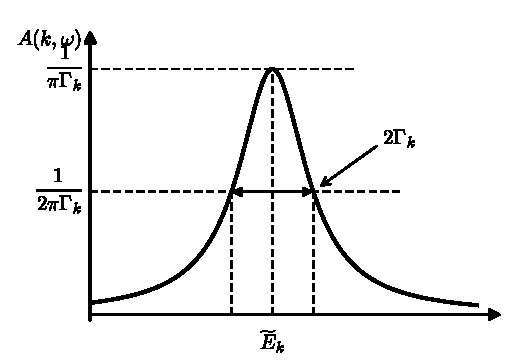
\includegraphics[width=7.5cm]{figD-1.pdf}\\{\small 图 D.1\quad 电子的谱函数}
\end{minipage}
\end{center}

\begin{equation}
1/\tau_{k}=2\Gamma_{k}\equiv-2\,\mathrm{Im}\Sigma_{\mathrm{r}}
(\boldsymbol{k},\omega=\widetilde{E}_{k})
\end{equation}
这是一个重要的关系式，在第四章§11中，我们将利用无规相近似介电函数计算寿命，然后由上式决定
$\mathrm{Im}\Sigma_{\mathrm{r}}(\boldsymbol{k},\widetilde{E}_{k})$.

% ============================================================
%  附录E 泊松求和公式
%  底本：高等教育出版社《固体理论》第二版；原书印刷页 552–553
%  （PDF 页 = 印刷页 + 20）
%  公式编号自检：(E.1)–(E.10)，自动编号 10 个，无缺号。
%
%  已修正的 OCR/原书错误（除全角句点转"."、删 ~ 间隔符、收紧
%  \mathrm{d}、拆开行内公式与中文等常规项外）：
%  1. (E.2) 括注 OCR 乱码"( n Σ*Σ )"按 p552 复原为"(n 为整数)"。
%  2. (E.5) 两处 lim 下标 OCR 丢箭头，按 p552 补"z→iω_n"。
%  3. 正文"[−βf(z)]"两处 OCR 乱码（\mathbf{\Lambda} 等）按
%     p552 复原。
%  4. 图 E.1 图例两行 OCR 乱码按 p552 复原为
%     ""×"——f(z)的极点，""·"——(z−x)^{-1}的极点"。
%  5. (E.7) 前文"沿实轴的上岸从−∞→∞"OCR 丢箭头按 p553 补；
%     "只包含 z=x 处的极点"OCR 乱码按 p553 复原。
%  6. (E.9) 首行及其前文的函数"[tanh(1/2)βx]/x"OCR 误作 βα，
%     按 p553 复原为 βx。
%  7. (E.9) 后文"对正 n 值求和"OCR 衍出"$f$"（成"求 f 和"），
%     按 p553 删。
%  8. 章末句"临界磁场 H_c(T)"后按 p553 补句点。
%  插图：图 E.1 泊松求和公式的回路（原书印刷 p552/PDF p572），
%  占位图 figures/figE-1.pdf（由 MinerU 裁剪图转 PDF 生成），
%  图例两行随图排。
%  遗留问题：无
% ============================================================
\chapter{泊松求和公式}

费密分布函数的下列级数展开式称为泊松(Poisson)求和公式
\begin{equation}
  f(x)=\frac{1}{\mathrm{e}^{\beta x}+1}
  =\frac{1}{\beta}\sum_{n=-\infty}^{\infty}
  \frac{\mathrm{e}^{\mathrm{i}\omega_{n}\eta}}{\mathrm{i}\omega_{n}-x}
\end{equation}
其中 $\beta=(k_{\mathrm{B}}T)^{-1}$，$\eta=+0$，而
\begin{equation}
  \omega_{n}\equiv(2n+1)\pi k_{\mathrm{B}}T
  \qquad(\text{$n$ 为整数})
\end{equation}
式(E.1)是一个有用的计算公式，其证明如下：

由于
\begin{equation}
  \mathrm{e}^{\mathrm{i}\beta\omega_{n}}
  =\mathrm{e}^{\mathrm{i}(2n+1)\pi}=-1
\end{equation}
因此，在 $z$ 复平面中费密函数可写成
\begin{equation}
  f(z)=\frac{1}{\mathrm{e}^{\beta z}+1}
  =\frac{1}{1-\mathrm{e}^{\beta(z-\mathrm{i}\omega_{n})}}
\end{equation}
它在虚轴上 $z=\mathrm{i}\omega_{n}$ 有奇点，这些奇点对称分布在实轴上下，如图E.1中“$\times$”号点所示.不难证实，$[-\beta f(z)]$ 函数有一组留数为1的极点，因为
\begin{equation}
  \lim_{z\to\mathrm{i}\omega_{n}}(z-\mathrm{i}\omega_{n})
  \left[-\beta f(z)\right]
  =\lim_{z\to\mathrm{i}\omega_{n}}
  \frac{(-\beta)(z-\mathrm{i}\omega_{n})}
  {1-\mathrm{e}^{\beta(z-\mathrm{i}\omega_{n})}}=1
\end{equation}
这时沿回路 $C$ 的下列积分可以用 $[-\beta f(z)]$ 的留数表示，得到等式
\begin{equation}
  \frac{1}{2\pi\mathrm{i}}\int_{C}\mathrm{d}z
  \frac{f(z)\mathrm{e}^{z\eta}}{z-x}
  =-\frac{1}{\beta}\sum_{n=-\infty}^{\infty}
  \frac{\mathrm{e}^{\mathrm{i}\omega_{n}\eta}}{\mathrm{i}\omega_{n}-x}
\end{equation}
由于公式(E.6)左边被积函数 $\left[f(z)\mathrm{e}^{z\eta}/(z-x)\right]$ 在 $z$ 复平面中（除实轴和虚轴以外的地方）是解析函数，因此利用约当(Jordan)引理可将沿回路 $C$ 的积分换为沿 $\Gamma+C'$ 回路的积分，这里 $\Gamma$ 是半径趋向无穷大的圆弧.考虑到 $\mathrm{e}^{z\eta}$ 因子的存在，当 $\mathrm{Re}\,z<0$ 时沿左半复平面 $\Gamma$ 上的被积函数将指数式趋向零.对于 $\mathrm{Re}\,z>0$ 情况，被积函数中的 $f(z)$ 将提供 $\mathrm{e}^{-\beta z}$ 因子，同样使得沿右半复平面的 $\Gamma$ 积分为零.

\begin{center}
\begin{minipage}{6.5cm}
\centering
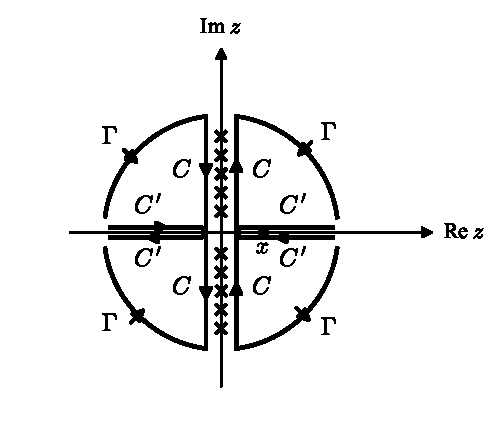
\includegraphics[width=6.5cm]{figE-1.pdf}\\*[0.3em]
{\small “$\times$”——$f(z)$的极点，}\\*[0.2em]
{\small “$\cdot$”——$(z-x)^{-1}$的极点}\\*[0.2em]
{\small 图 E.1\quad 泊松求和公式的回路}
\end{minipage}
\end{center}

这样可求出关系式
\begin{equation}
  \frac{1}{2\pi\mathrm{i}}\int_{C}\mathrm{d}z
  \frac{f(z)\mathrm{e}^{z\eta}}{z-x}
  =\frac{1}{2\pi\mathrm{i}}\int_{C'}\mathrm{d}z
  \frac{f(z)\mathrm{e}^{z\eta}}{z-x}
\end{equation}
式(E.7)相当于把绕虚轴的回路 $C$ 扭曲为 $C'$ 回路，使积分沿实轴的上岸从 $-\infty\to\infty$，然后再从实轴的下岸回到 $-\infty$ 处，由于沿 $C'$ 回路只包含 $z=x$ 处的极点，因此
\begin{equation}
  f(x)=-\frac{1}{2\pi\mathrm{i}}\int_{C'}\mathrm{d}z
  \frac{f(z)\mathrm{e}^{z\eta}}{z-x}
\end{equation}
再利用式(E.6)和(E.7)，即得泊松求和公式(E.1).

利用泊松求和公式可将函数 $\left[\tanh\frac{1}{2}\beta x\right]/x$ 表示为
\begin{equation}
\begin{aligned}
  \frac{\tanh\frac{1}{2}\beta x}{x}
  &=\frac{f(-x)-f(x)}{x}\\
  &=\frac{1}{\beta}\sum_{n=-\infty}^{\infty}
  \mathrm{e}^{\mathrm{i}\omega_{n}\eta}\frac{1}{x}
  \left[\frac{1}{\mathrm{i}\omega_{n}+x}
  -\frac{1}{\mathrm{i}\omega_{n}-x}\right]\\
  &=\frac{2}{\beta}\sum_{n=-\infty}^{\infty}
  \frac{\mathrm{e}^{\mathrm{i}\omega_{n}\eta}}
  {\omega_{n}^{2}+x^{2}}
\end{aligned}
\end{equation}
由于 $f$ 函数的极点对称分布于实轴上下，式(E.9)可简化为对正 $n$ 值求和，再考虑到 $\eta=+0$，从式(E.9)求出下列有用公式
\begin{equation}
  \frac{\tanh\frac{1}{2}\beta x}{x}
  =\frac{4}{\beta}\sum_{n=0}^{\infty}
  \frac{1}{\omega_{n}^{2}+x^{2}}
\end{equation}
上式在超导理论中用于计算 $T\to T_{\mathrm{c}}$ 时的能隙 $\Delta(T)$ 和临界磁场 $H_{\mathrm{c}}(T)$.

% ============================================================
%  附录F 相干态
%  底本：高等教育出版社《固体理论》第二版；原书印刷页 554–556
%  （PDF 页 = 印刷页 + 20）
%  公式编号自检：(F.1)–(F.16)，自动编号 16 个，无缺号。
%
%  已修正的 OCR/原书错误（除全角句点转"."、删 ~ 间隔符、拆开
%  行内公式与中文等常规项外）：
%  1. 原书 p554 (F.8) 第一行印 e^{-αâ⁺}|0>，与其第二行级数
%     Σαⁿ/√n!|n> 及本征方程(F.7)矛盾（e^{-αâ⁺}|0> 的展开为
%     Σ(−α)ⁿ/√n!|n>，本征值应为 −α），系原书排印漏正号，已按
%     物理改排为 e^{αâ⁺}|0> 并在此存照。
%  2. p555 段首"相于态"→"相干态"（OCR 误识）。
%  3. 原书 p555 "它代最小的不确定态"漏"表"字，按文义补为
%     "它代表最小的不确定态"（原书排印漏字，存照）。
%  4. "现在对算符 x̂ 和 p̂ 作相干态平均"OCR 语序错乱按 p555
%     复原；(F.9) 前文"非厄米算符 â"等处 OCR 重复/错位已清理。
%  5. (F.16) 后一段"非厄米算符 â 的非线性方程表示为"OCR 把 â
%     衍入"方程"一词中间，按 p555–556 复原；跨页断词"相干态方
%     法"已接排。
%  6. (F.1) 原书印 a⁺a（算符无帽），与 (F.2)(F.3) 的 â⁺â 不一致，
%     系原书照排，未改。
%  章末按原书照录参考书一句（倪光炯、陈苏卿《高等量子力学》）。
%  遗留问题：无
% ============================================================
\chapter{相干态}

频率为 $\omega$ 的振子哈密顿量为
\begin{equation}
  H_{0}=\hbar\omega\left(a^{+}a+\frac{1}{2}\right)
\end{equation}
振动量子的数算符定义为
\begin{equation}
  \hat{n}\equiv\hat{a}^{+}\hat{a}
\end{equation}
其本征方程可写成
\begin{equation}
  \hat{a}^{+}\hat{a}|n\rangle=n|n\rangle
  \qquad(n=0,1,2,\cdots)
\end{equation}
$|n\rangle$ 代表有确定量子数 $n$ 的状态，有关系式
\begin{equation}
\begin{gathered}
  |n\rangle=\frac{1}{\sqrt{n!}}
  \left(\hat{a}^{+}\right)^{n}|0\rangle\\
  \hat{a}|n\rangle=\sqrt{n}\,|n-1\rangle
  ,\qquad
  \hat{a}^{+}|n\rangle=\sqrt{n+1}\,|n+1\rangle
\end{gathered}
\end{equation}
态 $|n\rangle$ 所对应的振子波函数
\begin{equation}
  \langle x|n\rangle=\left(\sqrt{\pi}\,2^{n}n!\right)^{-\frac{1}{2}}
  \mathrm{H}_{n}(x)\exp\left(-x^{2}/2\right)
\end{equation}
其中
\begin{equation}
  \mathrm{H}_{n}(x)=(-1)^{n}\mathrm{e}^{x^{2}}
  \left(\frac{\mathrm{d}}{\mathrm{d}x}\right)^{n}
  \mathrm{e}^{-x^{2}}
\end{equation}
是 $n$ 阶厄米(Hermite)多项式.

相干态定义为非厄米算符 $\hat{a}$ 的本征态，它满足方程
\begin{equation}
  \hat{a}|\alpha\rangle=\alpha|\alpha\rangle
\end{equation}
其中 $\alpha$ 为复量.满足上式的相干态 $|\alpha\rangle$ 取下列形式：
\begin{equation}
\begin{aligned}
  |\alpha\rangle
  &=\mathrm{e}^{-|\alpha|^{2}/2}\,
  \mathrm{e}^{\alpha\hat{a}^{+}}|0\rangle\\
  &=\mathrm{e}^{-|\alpha|^{2}/2}\sum_{n=0}^{\infty}
  \frac{\alpha^{n}}{\sqrt{n!}}\,|n\rangle
\end{aligned}
\end{equation}
不难证实，若用算符 $\hat{a}$ 作用于 $|\alpha\rangle$ 将得到本征方程(F.7)
\begin{equation*}
\begin{aligned}
  \hat{a}|\alpha\rangle
  &=\mathrm{e}^{-|\alpha|^{2}/2}\sum_{n=0}^{\infty}
  \frac{\alpha^{n}}{\sqrt{n!}}\,\hat{a}|n\rangle\\
  &=\alpha\,\mathrm{e}^{-|\alpha|^{2}/2}\sum_{n=1}^{\infty}
  \frac{\alpha^{n-1}}{\sqrt{(n-1)!}}\,|n-1\rangle\\
  &=\alpha|\alpha\rangle
\end{aligned}
\end{equation*}
因此，$|\alpha\rangle$ 的表示式(F.8)是非厄米算符 $\hat{a}$ 的本征态，其本征值
\begin{equation}
  \alpha=\langle\alpha|\hat{a}|\alpha\rangle
\end{equation}
应当注意，相干态 $|\alpha\rangle$ 不再是具有确定量子数的状态 $|n\rangle$，而是各种 $n$ 的特殊组合态.式(F.8)的第二个等式表明了在谐振子情况下 $|\alpha\rangle$ 与 $|n\rangle$ 的关系.

相干态的另一个重要特征是，它代表最小的不确定态，也可以说是最经典的量子态.众所周知，任意可观察量 $\hat{A}$ 与 $\hat{B}$ 对于一般态 $|\psi\rangle$ 的量子力学平均值 $\langle\hat{A}\rangle=\langle\psi|\hat{A}|\psi\rangle$，若定义 $\Delta\hat{A}=\hat{A}-\langle\hat{A}\rangle$，则均方偏差 $\langle(\Delta\hat{A})^{2}\rangle=\langle\hat{A}^{2}\rangle-(\langle\hat{A}\rangle)^{2}$，在量子力学中已知，可观察量 $\hat{A}$ 与 $\hat{B}$ 之间存在下列不确定关系：
\begin{equation}
  \langle(\Delta\hat{A})^{2}\rangle
  \langle(\Delta\hat{B})^{2}\rangle
  \geqslant\frac{1}{4}
  \left|\langle[\hat{A},\hat{B}]\rangle\right|^{2}
\end{equation}
对于简谐振子系统 $\hat{H}=\frac{1}{2m}\hat{p}^{2}
+\frac{1}{2}m\omega^{2}\hat{x}^{2}$，其中
\begin{equation}
  \hat{x}=\left(\hbar/2m\omega\right)^{1/2}
  \left(\hat{a}^{+}+\hat{a}\right)
  ,\qquad
  \hat{p}=\mathrm{i}\left(m\hbar\omega/2\right)^{1/2}
  \left(\hat{a}^{+}-\hat{a}\right)
\end{equation}
若取 $\hat{A}=\hat{x}$ 与 $\hat{B}=\hat{p}$，因为 $[\hat{x},\hat{p}]=\mathrm{i}\hbar$，代入式(F.10)可求得简谐振子的不确定关系为
\begin{equation}
  \langle(\Delta\hat{x})^{2}\rangle
  \langle(\Delta\hat{p})^{2}\rangle
  \geqslant\frac{1}{4}\hbar^{2}
\end{equation}
当上式中等号成立时称为最小不确定态.现在对算符 $\hat{x}$ 和 $\hat{p}$ 作相干态平均，利用式(F.7)不难算得
\begin{equation}
\begin{aligned}
  &\langle\alpha|\hat{x}|\alpha\rangle
  =\left(\hbar/2m\omega\right)^{1/2}
  \left(\alpha^{*}+\alpha\right)
  ,\\
  &\langle\alpha|\hat{p}|\alpha\rangle
  =-\mathrm{i}\left(m\hbar\omega/2\right)^{1/2}
  \left(\alpha^{*}-\alpha\right)
\end{aligned}
\end{equation}
相应的
\begin{equation}
\begin{aligned}
  &\langle\alpha|\hat{x}^{2}|\alpha\rangle
  =\left(\hbar/2m\omega\right)
  \left[\left(\alpha^{*}+\alpha\right)^{2}+1\right]\\
  &\langle\alpha|\hat{p}^{2}|\alpha\rangle
  =-\left(m\hbar\omega/2\right)
  \left[\left(\alpha^{*}-\alpha\right)^{2}-1\right]
\end{aligned}
\end{equation}
这时，在相干态中，简谐振子的均方偏差为
\begin{equation}
\begin{aligned}
  &\langle(\Delta\hat{x})^{2}\rangle_{\mathrm{c}}
  \equiv\langle\alpha|(\Delta x)^{2}|\alpha\rangle\\
  &\qquad=\langle\alpha|\hat{x}^{2}|\alpha\rangle
  -\left(\langle\alpha|\hat{x}|\alpha\rangle\right)^{2}
  =\left(\hbar/2m\omega\right)\\
  &\langle(\Delta\hat{p})^{2}\rangle_{\mathrm{c}}
  \equiv\langle\alpha|(\Delta p)^{2}|\alpha\rangle
  =\left(m\hbar\omega/2\right)
\end{aligned}
\end{equation}
最后，求得简谐振子在相干态中的均方偏差满足最小不确定关系：
\begin{equation}
  \langle(\Delta\hat{x})^{2}\rangle_{\mathrm{c}}
  \langle(\Delta\hat{p})^{2}\rangle_{\mathrm{c}}
  =\frac{1}{4}\hbar^{2}
\end{equation}
因此，相干态是最小的不确定态.在非线性问题中，相干态将作为一种表象被应用，这时可利用式(F.9)将非厄米算符 $\hat{a}$ 的非线性方程表示为它的相干态平均值方程.在本书第三章中将应用相干态方法讨论一维铁磁链中的孤子运动问题，这是一种良好的准经典近似方法.

有关相干态的详细讨论，读者可参阅倪光炯、陈苏卿的《高等量子力学》（复旦大学出版社，2000年3月）.

% ============================================================
%  附录G 薛定谔方程的变分原理
%  底本：高等教育出版社《固体理论》第二版；原书印刷页 557–558
%  （PDF 页 = 印刷页 + 20）
%  公式编号自检：(G.1)–(G.15)，自动编号 15 个，无缺号
%  （任务单所称缺 [11] 系 OCR 把 (G.11) 的 tag 残缺为"(.11)"
%  未被脚本计入，原书 p558 在号）。
%
%  已修正的 OCR/原书错误（除全角句点转"."、收紧 \mathrm{d}、
%  拆开行内公式与中文等常规项外）：
%  1. [定理]句及"将 φ(r) 代入能量泛函"OCR 作 φ(r)，按 p557
%     原书复原为 ψ(r)。
%  2. (G.3) 势能项与分母 OCR 作 |φ(r)|²、|φ,(r)|²，按 p557
%     原书复原为 |ψ(r)|²（原书全式均排 ψ）。
%  3. (G.11) 前一未编号式 OCR 的"∇φ_k、φ_k"按 p557–558 复原为
%     ∇ψ_k、ψ_k；该块首行"F[∮φ,ψ_k]"乱码按 p557 复原为
%     F[φ,ψ_k]。
%  4. (G.11) tag 残缺"(.11)"已归还本式；其首行括号
%     "( −∇²u_k−2ik·∇u_k+k²u_k )"OCR 乱码按 p558 复原。
%  5. (G.13)(G.14) OCR 作 φ、φ_k、δ̂φ，按 p558 原书复原为
%     ψ、ψ_k、δψ（原书两式均排 ψ，δ 无帽）。
%  6. (G.4) 原书印"0(δψ)²"（数字零），(G.13)–(G.15) 印
%    "O(δψ)²"（字母 O），照原书分别照录，未统一。
%  正文引用 (1.5.13)、(1.5.22) 照录（指第一章式号）。
%  遗留问题：无
% ============================================================
\chapter{薛定谔方程的变分原理}

[定理] 设 $\psi(\boldsymbol{r})$ 是满足布洛赫定理的一次可微变分函数
\begin{equation}
  \psi=\psi_{k}+\delta\psi
\end{equation}
$\delta\psi$ 为小量，$\psi_{k}$ 是周期场中单电子薛定谔方程的解
\begin{equation}
  -\frac{\hbar^{2}}{2m}\nabla^{2}\psi_{k}
  +V(\boldsymbol{r})\psi_{k}=E_{k}\psi_{k}
\end{equation}
代表 $k$ 波矢和 $E_{k}$ 能量的布洛赫函数.将 $\psi(\boldsymbol{r})$ 代入能量泛函
\begin{equation}
  E[\psi]=\frac{\displaystyle\int\mathrm{d}\tau\left(
  \frac{\hbar^{2}}{2m}\left|\nabla\psi(\boldsymbol{r})\right|^{2}
  +V(\boldsymbol{r})\left|\psi(\boldsymbol{r})\right|^{2}\right)}
  {\displaystyle\int\mathrm{d}\tau
  \left|\psi(\boldsymbol{r})\right|^{2}}
\end{equation}
可证明
\begin{equation}
  E[\psi]=E[\psi_{k}]+0\,(\delta\psi)^{2}
\end{equation}
其中
\begin{equation}
  E[\psi_{k}]=E_{k}
\end{equation}
由于(G.4)中不含 $\delta\psi$ 一次项，说明能量泛函 $E[\psi]$ 对于式(G.1)所规定的 $\psi$ 是稳定的，而式(G.5)表明，稳定点的能量泛函值就是薛定谔方程(G.2)的能量本征值.

[证明] 为使记号简单起见定义
\begin{equation}
  F[\phi,\chi]\equiv\int\mathrm{d}\tau\left(
  \frac{\hbar^{2}}{2m}\nabla\phi^{*}\cdot\nabla\chi
  +V(\boldsymbol{r})\phi^{*}\chi\right)
\end{equation}
\begin{equation}
  (\phi,\chi)\equiv\int\mathrm{d}\tau\,\phi^{*}\chi
\end{equation}
这样 $E[\psi]$ 简记为
\begin{equation}
  E[\psi]=\frac{F[\psi,\psi]}{(\psi,\psi)}
\end{equation}
设 $\phi$ 为满足 $k$ 波矢的布洛赫定理的任意函数
\begin{equation}
  \phi(\boldsymbol{r})=v(\boldsymbol{r})
  \mathrm{e}^{\mathrm{i}\boldsymbol{k}\cdot\boldsymbol{r}}
\end{equation}
而
\begin{equation}
  \psi_{k}(\boldsymbol{r})=u_{k}(\boldsymbol{r})
  \mathrm{e}^{\mathrm{i}\boldsymbol{k}\cdot\boldsymbol{r}}
\end{equation}
其中 $u_{k}(\boldsymbol{r})$ 与 $v(\boldsymbol{r})$ 都是正点阵的周期函数，于是
\begin{equation*}
\begin{aligned}
  F[\phi,\psi_{k}]
  &=\int\mathrm{d}\tau\left(\frac{\hbar^{2}}{2m}
  \nabla\phi^{*}\cdot\nabla\psi_{k}
  +V\phi^{*}\psi_{k}\right)\\
  &=\frac{\hbar^{2}}{2m}\Bigl\{k^{2}\int\mathrm{d}\tau\,
  v^{*}u_{k}
  +\mathrm{i}\boldsymbol{k}\cdot\int\mathrm{d}\tau\,
  \left(u_{k}\nabla v^{*}-v^{*}\nabla u_{k}\right)\\
  &\qquad+\int\mathrm{d}\tau\,\nabla v^{*}\cdot\nabla u_{k}
  \Bigr\}+\int\mathrm{d}\tau\,V\phi^{*}\psi_{k}
\end{aligned}
\end{equation*}
对于周期函数 $v^{*}$ 和 $u_{k}$ 利用式(1.5.13)，对于 $\nabla v^{*}$ 和 $\nabla u_{k}$ 应用式(1.5.22)，求得
\begin{equation}
\begin{aligned}
  F[\phi,\psi_{k}]
  &=\frac{\hbar^{2}}{2m}\int\mathrm{d}\tau\,v^{*}
  \left(-\nabla^{2}u_{k}
  -2\mathrm{i}\boldsymbol{k}\cdot\nabla u_{k}
  +k^{2}u_{k}\right)
  +\int\mathrm{d}\tau\,V\phi^{*}\psi_{k}\\
  &=-\frac{\hbar^{2}}{2m}\int\mathrm{d}\tau\,\phi^{*}
  \nabla^{2}\psi_{k}
  +\int\mathrm{d}\tau\,V\phi^{*}\psi_{k}\\
  &=\int\mathrm{d}\tau\,\phi^{*}\left[-\frac{\hbar^{2}}{2m}
  \nabla^{2}+V(\boldsymbol{r})\right]\psi_{k}\\
  &=E_{k}\left(\phi,\psi_{k}\right)
\end{aligned}
\end{equation}
类似的方法可证明
\begin{equation}
  F[\psi_{k},\phi]=E_{k}\left(\psi_{k},\phi\right)
\end{equation}
现将式(G.1)代入式(G.6)，再利用式(G.11)与式(G.12)，求得
\begin{equation}
\begin{aligned}
  F[\psi,\psi]
  &=F[\psi_{k}+\delta\psi,\psi_{k}+\delta\psi]\\
  &=F[\psi_{k},\psi_{k}]+F[\delta\psi,\psi_{k}]
  +F[\psi_{k},\delta\psi]+O\left(\delta\psi\right)^{2}\\
  &=E_{k}\left\{(\psi_{k},\psi_{k})+(\psi_{k},\delta\psi)
  +(\delta\psi,\psi_{k})\right\}
  +O\left(\delta\psi\right)^{2}
\end{aligned}
\end{equation}
又由于
\begin{equation}
  (\psi,\psi)=(\psi_{k},\psi_{k})+(\psi_{k},\delta\psi)
  +(\delta\psi,\psi_{k})+O\left(\delta\psi\right)^{2}
\end{equation}
最后，将式(G.13)与式(G.14)代入式(G.8)并作小量展开
\begin{equation}
  E[\psi]=\frac{F[\psi,\psi]}{(\psi,\psi)}
  =E_{k}+O\left(\delta\psi\right)^{2}
\end{equation}
当式(G.15)中取 $\delta\psi=0$，即得到 $E[\psi_{k}]=E_{k}$，于是变分原理式(G.4)与(G.5)得证.

应当特别指出，在证明过程并未要求变分函数 $\psi$ 的一阶导数连续（二次可微条件），因此本节的原理适用于对缀加平面波作变分计算.

% ============================================================
%  附录H 自旋密度算符
%  底本：高等教育出版社《固体理论》第二版；原书印刷页 559–560
%  （PDF 页 = 印刷页 + 20）
%  公式编号自检：(H.1)–(H.10)，自动编号 10 个，无缺号。
%
%  已修正的 OCR/原书错误（除全角句点转"."、删 ~ 间隔符等常规项外）：
%  1. (H.1) δ 函数 OCR 误识为"\otimes"，按 p559 复原为
%     δ(r−r_j)。
%  2. (H.1) 后文 OCR"其中r为电子坐标，r_j σ̂ 为…"语序错乱，
%     按 p559 复原为"其中 r_j 为电子坐标，σ̂ 为向量自旋泡利矩阵"。
%  3. (H.5) 求和下标 OCR 作 i，按 p559 原书 Σ_j 复原。
%  4. (H.6) 前文衍出的顿号（"、为求出"）按 p559 删。
%  5. (H.6) 后文"这里χ为自旋函数，χ_μ μ 代表自旋取向"语序
%     错乱，按 p559 复原为"这里 χ_μ 为自旋函数，μ 代表自旋取向"。
%  6. (H.7) 各行 C 系数上下标 OCR 错乱（δ_{k',k+q} 排成
%     \mathrm{u}、求和指标 i/j 混用等），已按 p559 原书逐行复原为
%     C⁺_{k'μ}C_{kν}(½σ̂_{μν})…δ_{k',k+q}…C⁺_{k+q,μ}C_{kν}。
%  7. (H.8)(H.9) OCR 乱码按 p559 复原：Ŝ^z(q)=Σ_k(1/2)
%     (C⁺_{k+q↑}C_{k↑}−C⁺_{k+q↓}C_{k↓})、Ŝ⁺(q)=Σ_k C⁺_{k+q↑}C_{k↓}。
%  8. 末句"Ŝ^±(q)代表横向自旋密度起伏"OCR 上标乱码，按 p560
%     复原为 ±。
%  (H.2) 中 σ̂⁺=(0 2;0 0)、σ̂⁻=(0 0;2 0) 系原书定义（矩阵元含
%  因子 2，与各式中 (1/2)σ̂ 相配），照录未改。
%  遗留问题：无
% ============================================================
\chapter{自旋密度算符}

$N$ 个电子系统的自旋密度算符定义为
\begin{equation}
  \hat{\boldsymbol{S}}(\boldsymbol{r})=\sum_{j}
  \delta(\boldsymbol{r}-\boldsymbol{r}_{j})
  \frac{1}{2}\hat{\boldsymbol{\sigma}}
\end{equation}
其中 $\boldsymbol{r}_{j}$ 为电子坐标，$\hat{\boldsymbol{\sigma}}$ 为向量自旋泡利矩阵：
\begin{equation}
  \hat{\sigma}^{z}=\begin{pmatrix}1&0\\0&-1\end{pmatrix}
  ,\qquad
  \hat{\sigma}^{+}=\begin{pmatrix}0&2\\0&0\end{pmatrix}
  ,\qquad
  \hat{\sigma}^{-}=\begin{pmatrix}0&0\\2&0\end{pmatrix}
\end{equation}
将 $\delta$ 函数作傅里叶展开：
\begin{equation}
  \delta(\boldsymbol{r}-\boldsymbol{r}_{j})=\frac{1}{N}
  \sum_{\boldsymbol{q}}\mathrm{e}^{-\mathrm{i}\boldsymbol{q}\cdot
  (\boldsymbol{r}-\boldsymbol{r}_{j})}
\end{equation}
代入式(H.1)，求得
\begin{equation}
  \hat{\boldsymbol{S}}(\boldsymbol{r})=\sum_{\boldsymbol{q}}
  \hat{\boldsymbol{S}}(\boldsymbol{q})
  \mathrm{e}^{-\mathrm{i}\boldsymbol{q}\cdot\boldsymbol{r}}
\end{equation}
其中自旋密度算符的傅里叶分量
\begin{equation}
  \hat{\boldsymbol{S}}(\boldsymbol{q})=\frac{1}{N}\sum_{j}
  \left(\frac{1}{2}\hat{\boldsymbol{\sigma}}\right)
  \mathrm{e}^{\mathrm{i}\boldsymbol{q}\cdot\boldsymbol{r}_{j}}
\end{equation}
为求出 $\hat{\boldsymbol{S}}(\boldsymbol{q})$ 的二次量子化表示式，取态矢量
\begin{equation}
  \Psi(\boldsymbol{r}_{j})=\frac{1}{\sqrt{V}}
  \sum_{\boldsymbol{k},\mu}
  \mathrm{e}^{\mathrm{i}\boldsymbol{k}\cdot\boldsymbol{r}_{j}}
  C_{\boldsymbol{k}\mu}\chi_{\mu}
\end{equation}
这里 $\chi_{\mu}$ 为自旋函数，$\mu$ 代表自旋取向，$V$ 为系统的体积，利用式(H.6)，求得 $\hat{\boldsymbol{S}}(\boldsymbol{q})$ 的二次量子化表示为
\begin{equation}
\begin{aligned}
  \hat{\boldsymbol{S}}(\boldsymbol{q})
  &=\frac{1}{N}\sum_{j}\int\Psi^{+}(\boldsymbol{r}_{j})
  \left(\frac{1}{2}\hat{\boldsymbol{\sigma}}\right)
  \mathrm{e}^{\mathrm{i}\boldsymbol{q}\cdot\boldsymbol{r}_{j}}
  \Psi(\boldsymbol{r}_{j})\mathrm{d}\boldsymbol{r}_{j}\\
  &=\sum_{\boldsymbol{k},\boldsymbol{k}'}\sum_{\mu,\nu}
  C^{+}_{\boldsymbol{k}'\mu}C_{\boldsymbol{k}\nu}
  \left(\frac{1}{2}\hat{\sigma}_{\mu\nu}\right)
  \frac{1}{V}\int\mathrm{e}^{\mathrm{i}(\boldsymbol{k}
  +\boldsymbol{q}-\boldsymbol{k}')\cdot\boldsymbol{r}_{j}}
  \mathrm{d}\boldsymbol{r}_{j}\\
  &=\sum_{\boldsymbol{k},\boldsymbol{k}'}\sum_{\mu,\nu}
  C^{+}_{\boldsymbol{k}'\mu}C_{\boldsymbol{k}\nu}
  \left(\frac{1}{2}\hat{\sigma}_{\mu\nu}\right)
  \delta_{\boldsymbol{k}',\boldsymbol{k}+\boldsymbol{q}}\\
  &=\sum_{\boldsymbol{k},\mu,\nu}
  C^{+}_{\boldsymbol{k}+\boldsymbol{q},\mu}
  C_{\boldsymbol{k}\nu}
  \left(\frac{1}{2}\hat{\sigma}_{\mu\nu}\right)
\end{aligned}
\end{equation}
因此
\begin{equation}
  \hat{S}^{z}(\boldsymbol{q})=\sum_{\boldsymbol{k}}
  \frac{1}{2}\left(C^{+}_{\boldsymbol{k}+\boldsymbol{q}\uparrow}
  C_{\boldsymbol{k}\uparrow}
  -C^{+}_{\boldsymbol{k}+\boldsymbol{q}\downarrow}
  C_{\boldsymbol{k}\downarrow}\right)
\end{equation}
\begin{equation}
  \hat{S}^{+}(\boldsymbol{q})=\sum_{\boldsymbol{k}}
  C^{+}_{\boldsymbol{k}+\boldsymbol{q}\uparrow}
  C_{\boldsymbol{k}\downarrow}
\end{equation}
\begin{equation}
  \hat{S}^{-}(\boldsymbol{q})=\sum_{\boldsymbol{k}}
  C^{+}_{\boldsymbol{k}+\boldsymbol{q}\downarrow}
  C_{\boldsymbol{k}\uparrow}
\end{equation}
其中 $\hat{S}^{\pm}(\boldsymbol{q})$ 代表横向自旋密度起伏，用于描述金属中的自旋波.


% ---------------- 习题 ----------------
% ============================================================
%  书末习题（原书印刷页 561–570；PDF 页 = 印刷页 + 20）
%  底本：高等教育出版社《固体理论》第二版
%  体例（已逐页核对原书 p581–p590）：原书习题区**不按章分组**，
%    十二章的习题自 1. 至 50. 连续编号排版，无"第一章…"组头，
%    故本文件不设组头（任务单所拟"按章分组、组内另起 1."与原书
%    版面不符，以原书为准）；习题内公式一律不编号；题内带编号
%    条目"(1)"照录，纯公式条目用 equation* 左侧缀"(n)"。
%
%  已修正的 OCR 错误（除全角句点转"."、删 ~、收紧 \mathrm{d}、
%  拆开与中文粘连的行内公式等常规项外，均对照 p581–p590 页面）：
%  1. 题1  k=Σ_j(n_j/N_j)b_j 分子上衍出的点状杂符已删（p581）。
%  2. 题3  OCR"Ω^α=(2π)³"按 p581 复原为 ΩΩ*=(2π)³。
%  3. 题4  ψ_{n,k+K} 尾部衍出的杂符";"已删（p581）。
%  4. 题6  ω 的误置粗体已去；a⁺ 按 p581 复原（OCR \textbf 乱码）。
%  5. 题7  ω_σ(k) 的 OCR 杂符 \stackrel{,}{(} 复原为 (k)（p581）。
%  6. 题8  极化矢量 OCR \ell_{kσ} 按原书复原为 e_{kσ}（p582）；
%      弹性波方程分量上标 u^{x,y,z} 照原书排。
%  7. 题9  OCR"ω_L = ε₀−ε_∞"语序错乱，按 p582 复原为"ω_L 与 ω_T
%      为纵、横波频率"；4πγ₁₂² 下标结构复原。
%  8. 题11 OCR c_m(T) 按原书复原为 C_m(T)（大写 C、正体下标，p582）。
%  9. 题12 ℋ_{u'}、J_{u'} 按原书复原为 ℋ_{ll'}、J_{ll'}；(2) 中第二
%      列矢 (0 1)_{l'} 按 p582 复原。
% 10. 题13 Ŝ^γŜ_{l'}^γ → Ŝ_l^yŜ_{l'}^y；cos[k*(l−l')] →
%      cos[k·(l−l')]；求和下标 ι → l（p582）。
% 11. 题14 晶场 OCR ±B_{A^±} 复原为 ±B_A；ħω_k^x → ħω_k^±（p582–583）。
% 12. 题16 "(h=1)"按原书复原为 (ħ=1)（两处，p583）。
% 13. 题18 ω₁ 项 b_{−k}⁺b_k⁺ 顺序照原书（OCR 衍空格清理，p583）。
% 14. 题19 (1) OCR"[[H,ρq],ρ−q] = − m"按 p583 复原为 −(Nq²/m)；
%      "严格本征值"OCR 乱码（→^j 格）复原。
% 15. 题21 ε^{RPA}(q,ω) 两处 OCR 乱码按 p584 重排；ℒ(q) 定义式
%      OCR"="复原为"≡"。
% 16. 题24 (2)"T→0 K"OCR 缺箭头已补（p584）。
% 17. 题26 关联函数两行式 OCR 严重乱码，按 p585 重排复原
%      （g_{↑↑}、F(r) 及 j₁ 球贝塞耳函数）。
% 18. 题27 散射矩阵元 cases 块（−V 能壳内/0 能壳外）按 p585 复原；
%      Δ(K) 分母 exp[2/(g(k_F,K)V)]−1 补回 V；g(k_F,K) 乱码复原。
% 19. 题28 提示语 OCR 缺左方括号，按 p585 补"［提示：…］"。
% 20. 题29 g_s(ξ)/g_n(0) 两行 cases OCR 乱码按 p585 复原。
% 21. 题31 tanh(½β£_k) 的 £ 按原书复原为 ξ（p586）。
% 22. 题32 条件"T ≪ T_c ≪ T_c"OCR 重衍 → T ≪ T_c；
%      H_c(0)=ΔΛ(0)√(4πg(0)) → H_c(0)=Δ(0)√(4πg(0))（p586）。
% 23. 题33 ⟨H̄_int(λ)⟩ 下标 OCR 误作 τ → T；G(λ) 定义式乱码按
%      p586 复原。
% 24. 题34 高温区条件 (T_c−T<T_c) 按原书复原为 (T_c−T≪T_c)（p586）。
% 25. 题37 指数因子 (n−1)²P²/ħ² 原书排印 n/η 混用，按题内定义的 η
%      统一为 (η−1)²P²/ħ²（p566–567）；"而 r 的坐标原点取在电子上"
%      OCR 漏 r 已补。
% 26. 题38 e^{-s}He^s → e^{−S}He^{S}（母函数 S 大写，p567）。
% 27. 题39 对角形式两行式 OCR 乱码按 p567 复原。
% 28. 题40 Σ_r(ω) 定义 OCR"\sum_{±}"→ Σ_k（p567）。
% 29. 题41 E_k=−Wcos k 的条件 OCR"∧π<−W⩽E_k⩽W"乱码按 p567 复原为
%      "或 −W⩽E_k⩽W"；(2) 谱函数 A(ω) 中的 δ 函数 OCR 误作
%      \hat{ω}，按 p568 复原；Ẽ_d 式中 √(W⁴+4B²) 乱码复原（p568）。
% 30. 题44 C⁺_{kd} → C⁺_{kσ}；"严格解"OCR 乱码（→^± 格）复原（p568）。
% 31. 题45 ρ_f 式 (1/2D)·V²/(ω−E_f)² 的分母平方 OCR 衍落，已归位（p569）。
% 32. 题46 自洽方程被积式 OCR"(σ−1/π)Im…"按 p569 复原为
%      (−1/π)Im G_cf(ω+iη)。
% 33. 题47 (2)"\dot{T}=0 K"→ T=0 K；√(Γ̃²+(E_f−μ)²) 式按 p570 复原。
% 34. 题48 无双占条件 OCR"n_i≠n_i≠"按 p570 复原为 n_{i↑}n_{i↓}=0；
%      n_{iσ̄}（σ 带横杠，两处）复原。
% 35. 题49 μ_B 下标 OCR 误作 8 → B；m≡⟨n_↑⟩−⟨n_↓⟩ 乱码复原（p570）。
%
%  遗留问题：
%  · 习题图 1（题7，原书 p581 右下）为占位图 figures/figx-1.pdf，
%    待重绘代理绘制（六角形简约区BZ，含 Γ、T、Σ、M、K 及直角标记）。
%  · 题36"当 γ≪1 时上式简化为式(9.2.9)"照原书排（p566）；按物理
%    推断疑为"γ≫k"之误，未改。
%  · 题46 n_t 下标照原书（与 ch11 的 n_t=每格点总电子数一致，未改）。
% ============================================================
\chapter*{习题}
\markboth{习题}{}
\addcontentsline{toc}{chapter}{习题}

{\heiti 1.} 设 $\boldsymbol{k}$ 与 $\boldsymbol{k}'$ 均为BZ中波矢，$\boldsymbol{l}=\sum_{i}l_{i}\boldsymbol{a}_{i}$，$\boldsymbol{k}=\sum_{j}\frac{n_{j}}{N_{j}}\boldsymbol{b}_{j}$，$N_{1}N_{2}N_{3}=N$.试直接证明下列正交关系
\begin{equation*}
\begin{aligned}
  &\text{(1)}\ \ N^{-1}\sum_{l}\mathrm{e}^{\pm\mathrm{i}(\boldsymbol{k}-\boldsymbol{k}')\cdot\boldsymbol{l}}=\delta_{\boldsymbol{k}\boldsymbol{k}'}\\
  &\text{(2)}\ \ N^{-1}\sum_{k\in\mathrm{BZ}}\mathrm{e}^{\pm\mathrm{i}\boldsymbol{k}\cdot(\boldsymbol{l}-\boldsymbol{l}')}=\delta_{\boldsymbol{l}\boldsymbol{l}'}
\end{aligned}
\end{equation*}

{\heiti 2.} 设 $f(\boldsymbol{r})$ 为正点阵的周期函数，证明当 $\boldsymbol{k}$ 不等于倒格矢 $\boldsymbol{K}$ 时
\begin{equation*}
  \int f(\boldsymbol{r})\,\mathrm{e}^{\mathrm{i}\boldsymbol{k}\cdot\boldsymbol{r}}\,\mathrm{d}\boldsymbol{r}=0
\end{equation*}

{\heiti 3.} 证明 $\Omega\Omega^{*}=(2\pi)^{3}$

{\heiti 4.} 试用平面波法论证布洛赫函数
\begin{equation*}
  \psi_{n,\boldsymbol{k}}(\boldsymbol{r})=\psi_{n,\boldsymbol{k}+\boldsymbol{K}}(\boldsymbol{r})
\end{equation*}
其中 $\boldsymbol{k}$ 为简约波矢，$\boldsymbol{K}$ 为倒格矢，$n$ 为带指标.

{\heiti 5.} 设晶格周期场 $V=0$，试应用布洛赫定理求简约区（BZ）中单电子的能量和状态波函数，并作出能带曲线的一维示意图.

{\heiti 6.} 讨论在均匀外电场 $\mathcal{E}$ 中质量为 $M$，带电量为 $e$ 和频率为 $\omega$ 的一维谐振子系统.试证用玻色算子 $a$ 与 $a^{+}$ 表示的哈密顿量为
\begin{equation*}
  H=\hbar\omega\Bigl(a^{+}a+\frac{1}{2}\Bigr)+\lambda\left(a+a^{+}\right)
\end{equation*}
其中 $\lambda=e\mathcal{E}\sqrt{\dfrac{\hbar}{2M\omega}}$.

{\heiti 7.} 讨论二维密排六角晶格的格波特性.设 $a$ 为晶格常数，$f$ 代表最近邻原子间的线弹性力常数，其简约区BZ如下图所示，求BZ中 $\Sigma$ 线（包括 $\Gamma$，$M$ 点）和 $T$ 线（包括 $\Gamma$，$K$ 点）上的：

(1) 动力矩阵 $D_{\alpha\beta}(\boldsymbol{k})=?$

(2) 格波频率 $\omega_{\sigma}(\boldsymbol{k})$ 和极化矢量 $\boldsymbol{e}_{k\sigma}=?$

\par\nopagebreak\noindent\begin{minipage}{\linewidth}\centering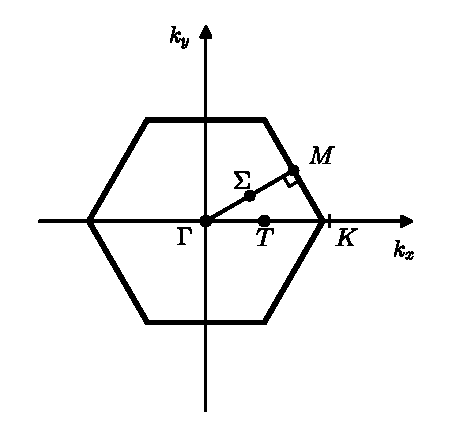
\includegraphics[width=4.5cm]{figx-1.pdf}\\[0.3em]{\small 习题图 1}\end{minipage}\par\nopagebreak

{\heiti 8.} 设立方晶体的弹性波方程为
\begin{equation*}
\begin{aligned}
  \rho\frac{\partial^{2}u^{x}}{\partial t^{2}}
  ={}&C_{11}\frac{\partial^{2}}{\partial x^{2}}u^{x}
  +C_{44}\Bigl(\frac{\partial^{2}}{\partial y^{2}}+\frac{\partial^{2}}{\partial z^{2}}\Bigr)u^{x}\\
  &+(C_{12}+C_{44})\frac{\partial}{\partial x}\Bigl(\frac{\partial u^{y}}{\partial y}+\frac{\partial u^{z}}{\partial z}\Bigr)
\end{aligned}
\end{equation*}
\begin{equation*}
\begin{aligned}
  \rho\frac{\partial^{2}u^{y}}{\partial t^{2}}
  ={}&C_{11}\frac{\partial^{2}}{\partial y^{2}}u^{y}
  +C_{44}\Bigl(\frac{\partial^{2}}{\partial z^{2}}+\frac{\partial^{2}}{\partial x^{2}}\Bigr)u^{y}\\
  &+(C_{12}+C_{44})\frac{\partial}{\partial y}\Bigl(\frac{\partial u^{z}}{\partial z}+\frac{\partial u^{x}}{\partial x}\Bigr)
\end{aligned}
\end{equation*}
\begin{equation*}
\begin{aligned}
  \rho\frac{\partial^{2}u^{z}}{\partial t^{2}}
  ={}&C_{11}\frac{\partial^{2}}{\partial z^{2}}u^{z}
  +C_{44}\Bigl(\frac{\partial^{2}}{\partial x^{2}}+\frac{\partial^{2}}{\partial y^{2}}\Bigr)u^{z}\\
  &+(C_{12}+C_{44})\frac{\partial}{\partial z}\Bigl(\frac{\partial u^{x}}{\partial x}+\frac{\partial u^{y}}{\partial y}\Bigr)
\end{aligned}
\end{equation*}
其中 $C_{ij}$ 为弹性常数，求沿 $[111]$ 方向的格波频率 $\omega_{\sigma}(\boldsymbol{k})$ 和极化矢量 $\boldsymbol{e}_{k\sigma}$.

{\heiti 9.} 设长波纵光学模的哈密顿密度为
\begin{equation*}
  \mathscr{H}_{0}=\frac{1}{2}\dot{\boldsymbol{W}}_{\mathrm{L}}^{2}
  +\frac{1}{2}\omega_{\mathrm{T}}^{2}\boldsymbol{W}_{\mathrm{L}}^{2}
  -\gamma_{12}\boldsymbol{W}_{\mathrm{L}}\cdot\boldsymbol{E}_{\mathrm{L}}
  -\frac{1}{2}\gamma_{22}\boldsymbol{E}_{\mathrm{L}}^{2}
\end{equation*}
其中 $E_{\mathrm{L}}=-\dfrac{4\pi\gamma_{12}}{1+4\pi\gamma_{22}}W_{\mathrm{L}}$，$1+4\pi\gamma_{22}=\varepsilon_{\infty}$，$4\pi\gamma_{12}^{2}=(\varepsilon_{0}-\varepsilon_{\infty})\omega_{\mathrm{T}}^{2}$，$\omega_{\mathrm{L}}$ 与 $\omega_{\mathrm{T}}$ 为纵、横波频率.试将系统的哈密顿量 $H_{0}=\int\mathscr{H}_{0}\,\mathrm{d}r$ 写成标准二次量子化形式.

{\heiti 10.} 利用色散关系式(2.2.30)计算一维双原子链的声子态密度，并作出声子频谱的示意图.

{\heiti 11.} 求立方晶格（sc、bcc、fcc）铁磁体中磁振子（magnons）的低温比热容 $C_{\mathrm{m}}(T)$.

{\heiti 12.} 讨论 $S=\frac{1}{2}$ 的两个自旋系统，设其哈密顿量为
\begin{equation*}
  \mathcal{H}_{ll'}=-2J_{ll'}\hat{\boldsymbol{S}}_{l}\cdot\hat{\boldsymbol{S}}_{l'}
\end{equation*}
试证明：

(1) $|\uparrow,\uparrow\rangle\equiv\binom{1}{0}_{\! l}\binom{1}{0}_{\! l'}$ 是 $\mathcal{H}_{ll'}$ 的本征态；

(2) $|\uparrow,\downarrow\rangle\equiv\binom{1}{0}_{\! l}\binom{0}{1}_{\! l'}$ 不是 $\mathcal{H}_{ll'}$ 的本征态.

{\heiti 13.} 若用
\begin{equation*}
  |k\rangle=\frac{1}{\sqrt{2SN}}\sum_{l}\mathrm{e}^{\mathrm{i}\boldsymbol{k}\cdot\boldsymbol{l}}\hat{S}_{l}^{-}|0\rangle
\end{equation*}
描述铁磁自旋晶格系统的最低激发态，试严格证明
\begin{equation*}
  \langle k|\bigl(\hat{S}_{l}^{x}\hat{S}_{l'}^{x}+\hat{S}_{l}^{y}\hat{S}_{l'}^{y}\bigr)|k\rangle
  =\frac{2S}{N}\cos\bigl[\boldsymbol{k}\cdot(\boldsymbol{l}-\boldsymbol{l}')\bigr]
\end{equation*}
并求系统的元激发能量 $\hbar\omega_{k}$，其中 $N$ 为格点数，$S$ 为格点上的自旋值，而 $|0\rangle$ 为铁磁基态.

{\heiti 14.} 证明在外磁场 $\boldsymbol{B}=\boldsymbol{B}\boldsymbol{z}$ 和各向异性晶场 $\pm\boldsymbol{B}_{A}$ 中（其中a子格取“+”号，b子格取“−”号）反铁磁体的自旋波量子为
\begin{equation*}
  \hbar\omega_{k}^{\pm}=2Z|J|S\sqrt{\Bigl(1+\frac{g\mu_{\mathrm{B}}B_{A}}{2Z|J|S}\Bigr)^{2}-\gamma_{k}^{2}}\pm g\mu_{\mathrm{B}}B
\end{equation*}
这里 $\gamma_{k}\equiv\frac{1}{2}\sum_{\boldsymbol{\delta}}^{\prime}\mathrm{e}^{-\mathrm{i}\boldsymbol{k}\cdot\boldsymbol{\delta}}$.

{\heiti 15.} 试用 $u-v$ 变换方法求
\begin{equation*}
  H=E_{0}a^{+}a+E_{1}\left(a^{+}a^{+}+aa\right)
\end{equation*}
的元激发严格解，其中 $a$ 与 $a^{+}$ 为玻色算子，$E_{0}$ 与 $E_{1}$ 为常数，且 $E_{0}>2E_{1}$.

{\heiti 16.} 设磁振子与声子互作用系统的哈密顿量为
\begin{equation*}
  H=\sum_{k}\bigl\{\bigl(\omega_{k}^{\mathrm{m}}a^{+}_{k}a_{k}
  +\omega_{k}^{\mathrm{p}}b^{+}_{k}b_{k}\bigr)
  +V_{k}\left(a_{k}b^{+}_{k}+a^{+}_{k}b_{k}\right)\bigr\}
\end{equation*}
其中 $\omega_{k}^{\mathrm{m}}$ 为磁振子能量（$\hbar=1$），$\omega_{k}^{\mathrm{p}}$ 为声子能量（$\hbar=1$），$a_{k}$ 为磁振子算符，$b_{k}$ 为声子算符，$V_{k}$ 为耦合系数，试求

(1) 使 $H$ 对角化的变换（变换形式及对角化条件）；

(2) 当 $\omega_{k}^{\mathrm{m}}=\omega_{k}^{\mathrm{p}}=\omega_{k}$ 时，互作用系统的元激发能量.

{\heiti 17.} 已知含 $N$ 个元胞复式晶格的电子TBA哈密顿量为
\begin{equation*}
  H=E_{1}\sum_{i}a^{+}_{i}a_{i}+E_{2}\sum_{j}b^{+}_{j}b_{j}
  +W\sum_{i}\sum_{\boldsymbol{\delta}}^{\prime}
  \left(a^{+}_{i}b_{i+\boldsymbol{\delta}}+b^{+}_{i}a_{i+\boldsymbol{\delta}}\right)
\end{equation*}
其中 $a_{i}$ 与 $b_{j}$ 是元胞中A、B原子周围的局域电子算符，晶格配位数设为 $Z$.试将 $H$ 对角化，并求出能带电子的能量.

{\heiti 18.} 设超流玻色系统的哈密顿量近似为
\begin{equation*}
  H=\sum_{k}^{\prime}\bigl\{\omega_{0}\bigl(b^{+}_{k}b_{k}+b^{+}_{-k}b_{-k}\bigr)
  +\omega_{1}\bigl(b_{k}b_{-k}+b^{+}_{-k}b^{+}_{k}\bigr)\bigr\}
\end{equation*}
其中 $\omega_{0}=\varepsilon_{k}+NV_{k}$，$\omega_{1}=NV_{k}$，$\varepsilon_{k}=\frac{k^{2}}{2M}$，$V_{k}>0$，$\sum_{k}^{\prime}(\cdots)$ 表示求和时 $k\neq0$.试将 $H$ 对角化，求出其元激发能量（取 $\hbar=1$ 单位），并讨论元激发谱中是否存在能隙？

{\heiti 19.} 证明互作用电子系统当取 $\hbar=1$ 时有下列严格关系：
\begin{equation*}
\begin{aligned}
  &\text{(1)}\ \ \bigl[\bigl[H,\rho_{\boldsymbol{q}}\bigr],\rho_{-\boldsymbol{q}}\bigr]
  =-\Bigl(\frac{Nq^{2}}{m}\Bigr);\\
  &\text{(2)}\ \ \sum_{n}\omega_{n0}\bigl\{\bigl|\langle n|\rho_{\boldsymbol{q}}|0\rangle\bigr|^{2}
  +\bigl|\langle n|\rho_{-\boldsymbol{q}}|0\rangle\bigr|^{2}\bigr\}=\frac{Nq^{2}}{m};\\
  &\text{(3)}\ \ \int_{0}^{\infty}\mathrm{d}\omega\,\omega\,
  \mathrm{Im}\Bigl[\frac{1}{\varepsilon(\boldsymbol{q},\omega)}\Bigr]
  =-\Bigl(\frac{\pi\omega_{\mathrm{p}}^{2}}{2}\Bigr),
\end{aligned}
\end{equation*}
其中 $\omega_{\mathrm{p}}^{2}=\frac{4\pi Ne^{2}}{m}$，$\rho_{\boldsymbol{q}}=\sum_{k}C^{+}_{k}C_{k+\boldsymbol{q}}$，$\omega_{n0}=\mathcal{E}_{n}-\mathcal{E}_{0}$，$\mathcal{E}_{n}$ 为 $H$ 的严格本征值.

{\heiti 20.} 利用附录B中的严格介电函数公式(B.1)，证明关系式
\begin{equation*}
  \lim_{\omega\to\infty}\mathrm{Re}\Bigl[\frac{1}{\varepsilon(\boldsymbol{q},\omega)}\Bigr]=1+\frac{\omega_{\mathrm{p}}^{2}}{\omega^{2}}
\end{equation*}

{\heiti 21.} 试用格林函数方法证明

(1) 哈特利-福克近似的介电函数
\begin{equation*}
  \frac{1}{\varepsilon^{\mathrm{HFA}}(\boldsymbol{q},\omega)}=1-\mathcal{L}(q)
\end{equation*}

(2) 无规相近似的介电函数
\begin{equation*}
  \varepsilon^{\mathrm{RPA}}(\boldsymbol{q},\omega)=1+\mathcal{L}(q)
\end{equation*}
其中
\begin{equation*}
  \mathcal{L}(q)\equiv\frac{v(q)}{\hbar}\sum_{k}n_{k}
  \Bigl\{\frac{1}{\omega_{kq}-(\omega+\mathrm{i}\eta)}
  +\frac{1}{\omega_{kq}+(\omega+\mathrm{i}\eta)}\Bigr\}
\end{equation*}
这里 $\eta=+0$.

{\heiti 22.} 证明三维电子气的等离激元的长波色散曲线为
\begin{equation*}
  \omega_{q}=\sqrt{\omega_{\mathrm{p}}^{2}+\frac{3}{5}q^{2}v_{\mathrm{F}}^{2}}
\end{equation*}
其中 $v_{\mathrm{F}}=\frac{\hbar k_{\mathrm{F}}}{m}$，$\omega_{\mathrm{p}}^{2}=\frac{4\pi Ne^{2}}{m}$.

{\heiti 23.} 求一维电子气 $q<2k_{\mathrm{F}}$ 时个别激发的下限 $\omega_{kq}^{\min}$，并在 $\omega-q$ 图上作出其曲线.

{\heiti 24.} 用介电函数讨论快速电子激发金属中等离激元的能量损失问题.设有一个速度为 $v$ 的快速电子注入金属.

(1) 证明此电子每秒的能量损耗为
\begin{equation*}
  -\Bigl(\frac{e}{\pi}\Bigr)^{2}\int\frac{\mathrm{d}^{2}q}{q^{2}}\int_{0}^{\infty}\mathrm{d}\omega\,\omega\,
  \mathrm{Im}\Bigl[\frac{1}{\varepsilon(\boldsymbol{q},\omega)}\Bigr]\delta(\omega-\boldsymbol{q}\cdot\boldsymbol{v})
\end{equation*}

(2) 试用无规相近似结果证明，当 $T\to0$ K 时在等离子集体振荡区（长波、高频限）
\begin{equation*}
  -\mathrm{Im}\Bigl[\frac{1}{\varepsilon^{\mathrm{RPA}}(q,\omega)}\Bigr]\approx\frac{\pi}{2}\omega_{\mathrm{p}}\delta(\omega-\omega_{\mathrm{p}})
\end{equation*}

{\heiti 25.} 试计算 $T>0$ K 时离子晶体中极化子的寿命 $\tau$.证明当 $k\ll\gamma\equiv(2m\omega_{\mathrm{L}}/\hbar)^{1/2}$ 时极化子在有限温度的
\begin{equation*}
  \frac{1}{\tau}\approx\frac{2\alpha\omega_{\mathrm{L}}}{\mathrm{e}^{\beta\hbar\omega_{\mathrm{L}}}-1}
\end{equation*}
讨论此结果的物理意义，其中 $\alpha$ 为极化子的耦合常数.

{\heiti 26.} 用哈特利-福克近似证明，在 $N$ 个电子系统中自旋平行电子对的关联函数
\begin{equation*}
\begin{aligned}
  &g_{\uparrow\uparrow}(\boldsymbol{r})=\frac{1}{N(N-1)}\sum_{i,j}
  \bigl|\phi_{\uparrow\uparrow}(\boldsymbol{r}_{i},\boldsymbol{r}_{j})\bigr|^{2}
  =\frac{1}{2}\bigl\{1-F^{2}(\boldsymbol{r})\bigr\}\\
  &F(\boldsymbol{r})=\frac{3}{k_{\mathrm{F}}r}\,j_{1}(k_{\mathrm{F}}r)
  =\frac{3}{(k_{\mathrm{F}}r)^{3}}\bigl[\sin(k_{\mathrm{F}}r)-(k_{\mathrm{F}}r)\cos(k_{\mathrm{F}}r)\bigr]
\end{aligned}
\end{equation*}
其中 $\boldsymbol{r}=\boldsymbol{r}_{i}-\boldsymbol{r}_{j}$、$\phi_{\uparrow\uparrow}(\boldsymbol{r}_{i},\boldsymbol{r}_{j})$ 代表自旋平行电子对哈特利-福克近似波函数的空间部分.

{\heiti 27.} 设总波矢为 $\boldsymbol{K}=\boldsymbol{k}_{1}+\boldsymbol{k}_{2}$ 的一对自旋反平行电子间的互作用势能为 $V(\boldsymbol{r})$，其散射矩阵元可近似写成
\begin{equation*}
\begin{aligned}
  V_{kk'}&=\frac{1}{N\Omega}\int V(\boldsymbol{r})\,
  \mathrm{e}^{\mathrm{i}(\boldsymbol{k}-\boldsymbol{k}')\cdot\boldsymbol{r}}\,\mathrm{d}\boldsymbol{r}\\
  &=\begin{cases}
    -V & \left(E_{\mathrm{F}}<E_{k}<E_{\mathrm{F}}+\hbar\omega_{\mathrm{D}}\text{，能壳内}\right)\\
    0 & \left(\text{能壳外}\right)
  \end{cases}
\end{aligned}
\end{equation*}
试证明电子对的能量
\begin{equation*}
  E=\frac{\hbar^{2}K^{2}}{4m}+\frac{\hbar^{2}k_{\mathrm{F}}^{2}}{m}-\Delta(\boldsymbol{K})
\end{equation*}
其中
\begin{equation*}
  \Delta(\boldsymbol{K})=\frac{2\hbar\omega_{\mathrm{D}}}{\exp\Bigl[\dfrac{2}{g(k_{\mathrm{F}},\boldsymbol{K})V}\Bigr]-1}
\end{equation*}
这里 $g(k_{\mathrm{F}},\boldsymbol{K})$ 代表费密面上总波矢为 $\boldsymbol{K}$ 的电子态密度.

{\heiti 28.} 证明库柏对的均方根半径
\begin{equation*}
  \sqrt{\langle r^{2}\rangle}\approx\frac{2}{\sqrt{3}}\,\frac{\hbar v_{\mathrm{F}}}{E}
\end{equation*}
［提示：库柏对是 $\boldsymbol{K}=0$ 的 $\uparrow$，$\downarrow$ 自旋电子对］

{\heiti 29.} 证明BCS超导体中准粒子的态密度 $g_{\mathrm{s}}(\xi)$ 与费密面上正常相态密度 $g_{\mathrm{n}}(0)$ 之比为
\begin{equation*}
  \frac{g_{\mathrm{s}}(\xi)}{g_{\mathrm{n}}(0)}=
  \begin{cases}
    \dfrac{\xi}{\sqrt{\xi^{2}-\Delta^{2}}} & \left(\left|\xi\right|>\Delta\right)\\[0.8em]
    0 & \left(\left|\xi\right|<\Delta\right)
  \end{cases}
\end{equation*}
其中 $\xi=\sqrt{\varepsilon^{2}+\Delta^{2}}$，$\varepsilon$ 为从费密面算起的自由电子能量.

{\heiti 30.} 试证明BCS超导体中总粒子数的涨落为
\begin{equation*}
  \frac{\langle\hat{N}^{2}\rangle-\langle\hat{N}\rangle^{2}}{\langle\hat{N}\rangle^{2}}
  =\frac{\displaystyle\sum_{k}\left(u_{k}v_{k}\right)^{2}}{\Bigl(\displaystyle\sum_{k}v_{k}^{2}\Bigr)^{2}}
\end{equation*}
其中 $\hat{N}=\sum_{k}\left(C^{+}_{k}C_{k}+C^{+}_{-k}C_{-k}\right)$，$\langle\cdots\rangle$ 代表对BCS基态的平均.

{\heiti 31.} 用BCS理论证明 $T>0$ K 时超导体中的平均占据数
\begin{equation*}
  \langle C^{+}_{k}C_{k}\rangle_{T}=\frac{1}{2}\Bigl[1-\bigl(\varepsilon_{k}/\xi_{k}\bigr)\tanh\Bigl(\frac{1}{2}\beta\xi_{k}\Bigr)\Bigr]
\end{equation*}

{\heiti 32.} 试用BCS理论证明超导体的临界磁场在 $T\ll T_{\mathrm{c}}$ 时为
\begin{equation*}
  H_{\mathrm{c}}(T)=H_{\mathrm{c}}(0)\Bigl(1-\frac{\mathrm{e}^{2\gamma}}{3}\,\frac{T^{2}}{T_{\mathrm{c}}^{2}}\Bigr)
\end{equation*}
其中 $H_{\mathrm{c}}(0)=\Delta(0)\sqrt{4\pi g(0)}$，$\gamma=0.5772$.

{\heiti 33.} 利用 $\overline{H}(\lambda)=\overline{H}_{0}+\overline{H}_{\mathrm{int}}(\lambda)$，$\overline{H}_{0}=H_{0}-\mu N$ 和 $\overline{H}_{\mathrm{int}}(\lambda)=\lambda\overline{H}_{\mathrm{int}}$ 以及吉布斯自由能 $G(\lambda)=-k_{\mathrm{B}}T\ln\mathrm{Tr}\left(\mathrm{e}^{-\beta\overline{H}(\lambda)}\right)$（其中 $\lambda=0$ 代表自由系统，$\lambda=1$ 为实际多体系统），试证明 $T>0$ K 时费因曼定理为
\begin{equation*}
  \frac{\partial G(\lambda)}{\partial\lambda}
  =\frac{\bigl\langle\overline{H}_{\mathrm{int}}(\lambda)\bigr\rangle_{T}}{\lambda}
\end{equation*}

{\heiti 34.} 试从式(6.8.50)导出伦敦穿透深度 $\lambda_{\mathrm{L}}(T)$ 在高温区和低温区的渐近式为
\begin{equation*}
  \Bigl[\frac{\lambda_{\mathrm{L}}(0)}{\lambda_{\mathrm{L}}(T)}\Bigr]^{2}\approx
  \begin{cases}
    2\left(1-T/T_{\mathrm{c}}\right) & \left(T_{\mathrm{c}}-T\ll T_{\mathrm{c}}\right)\\[0.5em]
    1-\sqrt{\dfrac{2\pi\Delta(0)}{k_{\mathrm{B}}T}}\,\mathrm{e}^{-\Delta(0)/k_{\mathrm{B}}T} & \left(T\ll T_{\mathrm{c}}\right)
  \end{cases}
\end{equation*}
其中 $\Delta(0)$ 为零温超导能隙，$\lambda_{\mathrm{L}}(0)$ 代表 $T=0$ K 时的伦敦穿透深度.

{\heiti 35.} 设在晶格常数 $a$ 的一维晶格中瓦尼尔表象的电子算符 $C_{l}$ 满足运动方程
\begin{equation*}
  \mathrm{i}\hbar\dot{C}_{l}=AC_{l}-B\left(C_{l-1}+C_{l+1}\right)
\end{equation*}
试求：

(1) 电子能量与波矢的关系 $E(k)$；

(2) 能带宽度和带顶空穴及带底电子的有效质量；

(3) $A=0$ 时能带电子的态密度 $\rho(E)$.

{\heiti 36.} 试用微扰论证明 $T=0$ K 时弗留里希极化子在 $\alpha\ll1$ 时的自能为
\begin{equation*}
  E_{k}=\varepsilon_{k}-\alpha\hbar\omega_{\mathrm{L}}\,
  \frac{\arcsin(k/\gamma)}{(k/\gamma)}
\end{equation*}
其中 $\varepsilon_{k}=\dfrac{\hbar^{2}k^{2}}{2m}$，$\gamma^{2}=\Bigl(\dfrac{2m\omega_{\mathrm{L}}}{\hbar}\Bigr)$，当 $\gamma\ll1$ 时上式简化为式(9.2.9).

{\heiti 37.} 证明LLP极化子中被电子感生的介质极化电荷密度为
\begin{equation*}
\begin{aligned}
  \rho(\boldsymbol{r})={}&\frac{em\omega_{\mathrm{L}}}{2\pi\hbar|\boldsymbol{r}|}
  \Bigl(\frac{1}{\varepsilon_{\infty}}-\frac{1}{\varepsilon_{0}}\Bigr)\times\\
  &\exp\Bigl\{-\Bigl[\gamma-\frac{(\eta-1)^{2}P^{2}}{\hbar^{2}}\Bigr]^{1/2}
  |\boldsymbol{r}|\Bigr\}
  \cos\Bigl[\frac{(\eta-1)\boldsymbol{P}\cdot\boldsymbol{r}}{\hbar}\Bigr]
\end{aligned}
\end{equation*}
其中 $\eta=\Bigl(\dfrac{\alpha}{6}\Bigr)\Big/\Bigl[1+\Bigl(\dfrac{\alpha}{6}\Bigr)\Bigr]$，$\gamma^{2}=\Bigl(\dfrac{2m\omega_{\mathrm{L}}}{\hbar}\Bigr)$，而 $\boldsymbol{r}$ 的坐标原点取在电子上.

{\heiti 38.} 试将习题6中一维带电谐振子的哈密顿量对角化，并求出位移振子变换
\begin{equation*}
  \overline{H}=\mathrm{e}^{-S}H\mathrm{e}^{S}
\end{equation*}
的母函数 $S$.

{\heiti 39.} 设电子与声子互作用系统的哈密顿量为
\begin{equation*}
  H=E_{0}C^{+}C+C^{+}C\sum_{q}M_{q}\left(a_{q}+a^{+}_{q}\right)
  +\sum_{q}\hbar\omega_{q}\Bigl(a^{+}_{q}a_{q}+\frac{1}{2}\Bigr)
\end{equation*}
其中 $C$ 为费密算子，$a_{q}$ 为玻色算子，$M_{q}$ 为实量.试用位移振子变换证明 $H$ 可写成下列对角形式：
\begin{equation*}
\begin{aligned}
  \overline{H}&=\mathrm{e}^{-S}H\mathrm{e}^{S}\\
  &=\Bigl(E_{0}-\sum_{q}\frac{M_{q}^{2}}{\hbar\omega_{q}}\Bigr)C^{+}C
  +\sum_{q}\hbar\omega_{q}\Bigl(a^{+}_{q}a_{q}+\frac{1}{2}\Bigr)
\end{aligned}
\end{equation*}
并求出变换的母函数 $S$.

{\heiti 40.} 试用格林函数运动方程方法严格求解范纳-安德逊（Fano-Anderson）模型：
\begin{equation*}
  H=\sum_{\sigma}E_{\mathrm{d}}d^{+}_{\sigma}d_{\sigma}
  +\sum_{k,\sigma}E_{k}C^{+}_{k\sigma}C_{k\sigma}
  +\sum_{k,\sigma}V_{k}\left(C^{+}_{k\sigma}d_{\sigma}+d^{+}_{\sigma}C_{k\sigma}\right).
\end{equation*}
证明局域d电子的态密度公式为
\begin{equation*}
  \rho_{\mathrm{d}}(\omega)=-\frac{1}{\pi}\,
  \frac{\mathrm{Im}\,\Sigma_{r}(\omega)}
  {\left(\omega-E_{\mathrm{d}}-\mathrm{Re}\,\Sigma_{r}(\omega)\right)^{2}
  +\left(\mathrm{Im}\,\Sigma_{r}(\omega)\right)^{2}}
\end{equation*}
其中 $\Sigma_{r}$ 为来自 $V_{k}$ 杂化项的推迟自能修正
\begin{equation*}
  \Sigma_{r}(\omega)=\sum_{k}\frac{V_{k}^{2}}{\omega-E_{k}+\mathrm{i}\eta}
  \qquad\left(\eta=0^{+}\right)
\end{equation*}

{\heiti 41.} 当不计及自旋效应时，上题中的哈密顿量简化为
\begin{equation*}
  H=E_{\mathrm{d}}d^{+}d+\sum_{k}E_{k}C^{+}_{k}C_{k}
  +\sum_{k}V_{k}\left(C^{+}_{k}d+d^{+}C_{k}\right)
\end{equation*}
设在长度为 $L$ 的一维晶体中，s-d杂化作用的强度取为
\begin{equation*}
  V_{k}^{2}=\frac{B}{L},
\end{equation*}
$B$ 是常数，导带电子能量取紧束缚近似能带值
\begin{equation*}
  E_{k}=-W\cos k\qquad
  \left(-\pi\leqslant k\leqslant\pi\ \text{或}\ -W\leqslant E_{k}\leqslant W\right)
\end{equation*}
这里设晶格常数 $a=1$.

(1) 试用格林函数运动方程方法算出此互作用系统的推迟自能实部（$\mathrm{Re}\,\Sigma_{r}$）与虚部（$\mathrm{Im}\,\Sigma_{r}$）分别在能带区内（$\omega^{2}\leqslant W^{2}$）及区外（$\omega^{2}>W^{2}$）的具体表达式.

(2) 根据附录D，在单杂质情况下，局域d电子的谱函数 $A_{\mathrm{d}}(\omega)$ 就是上题中的d电子的态密度.当未微扰的局域d电子的能级取 $E_{\mathrm{d}}=0$ 时，试证明其谱函数为
\begin{equation*}
  A(\omega)=
  \begin{cases}
    \delta\Bigl(\omega-\dfrac{B}{\sqrt{\omega^{2}-W^{2}}}\Bigr)
    +\delta\Bigl(\omega+\dfrac{B}{\sqrt{\omega^{2}-W^{2}}}\Bigr)
    & \left(\omega^{2}>W^{2}\right)\\[1em]
    \dfrac{B}{\pi}\cdot
    \dfrac{1}{\sqrt{W^{2}-\omega^{2}}\ \bigl[\omega^{2}+B^{2}/(W^{2}-\omega^{2})\bigr]}
    & \left(\omega^{2}\leqslant W^{2}\right)
  \end{cases}
\end{equation*}

(3) 以上结果表明，在能带区外 $\omega=\pm\widetilde{E}_{\mathrm{d}}$ 处存在真正的束缚态，试证明其中的
\begin{equation*}
  \widetilde{E}_{\mathrm{d}}=\frac{1}{\sqrt{2}}
  \bigl(W^{2}+\sqrt{W^{4}+4B^{2}}\bigr)^{1/2}
\end{equation*}

{\heiti 42.} 试用格林函数运动方程方法处理低激发近似下的反铁磁系统
\begin{equation*}
\begin{aligned}
  H={}&-2NZS^{2}|J|+2ZS|J|\Bigl(\sum_{i=1}^{N}a^{+}_{i}a_{i}
  +\sum_{j=1}^{N}b^{+}_{j}b_{j}\Bigr)\\
  &+2S|J|\sum_{i,\boldsymbol{\delta}}\bigl(a_{i}b_{i+\boldsymbol{\delta}}
  +a^{+}_{i}b^{+}_{i+\boldsymbol{\delta}}\bigr)
\end{aligned}
\end{equation*}
其中 $a_{i}$、$b_{j}$ 均为玻色算子，$N$ 为晶格元胞数，$\boldsymbol{\delta}$ 为近邻正格矢，$Z$ 为近邻配位数.试求反铁磁自旋波量子 $\hbar\omega_{k}=?$

{\heiti 43.} 试从自洽场近似的BCS约化哈密顿量
\begin{equation*}
  \overline{H}=\sum_{k}\varepsilon_{k}\left(C^{+}_{k}C_{k}+C^{+}_{-k}C_{-k}\right)
  -\Delta\sum_{k}\left(C^{+}_{k}C^{+}_{-k}+C_{-k}C_{k}\right)+\frac{\Delta^{2}}{V}
\end{equation*}
出发，利用格林函数运动方程方法，导出有限温度的超导能隙方程.这里 $\Delta=\Delta(T)=V\sum_{k}\langle C_{-k}C_{k}\rangle$ 代表超导能隙的定义.

{\heiti 44.} 试用格林函数运动方程方法求解下列传导电子与局域电子的互作用晶格系统
\begin{equation*}
  H=\sum_{k,\sigma}E_{k}C^{+}_{k\sigma}C_{k\sigma}
  +\sum_{i,\sigma}E_{\mathrm{f}}f^{+}_{i\sigma}f_{i\sigma}
  +\frac{V}{\sqrt{N}}\sum_{k,i,\sigma}
  \left(C^{+}_{k\sigma}f_{i\sigma}\mathrm{e}^{-\mathrm{i}\boldsymbol{k}\cdot\boldsymbol{R}_{i}}
  +f^{+}_{i\sigma}C_{k\sigma}\mathrm{e}^{\mathrm{i}\boldsymbol{k}\cdot\boldsymbol{R}_{i}}\right)
\end{equation*}
{\emergencystretch=3em
其中 $\boldsymbol{R}_{i}$ 是i格点的位置矢.试求传导电子与局域电子格林函数的严格解 $\langle\langle C_{k\sigma}|C^{+}_{k\sigma}\rangle\rangle_{\omega}=?$ 及 $\langle\langle f_{k\sigma}|f^{+}_{k\sigma}\rangle\rangle_{\omega}=?$ 并定出系统的元激发谱（即杂化带）.\par}

{\heiti 45.} 设上题中平均每格点上传导电子的未微扰态密度取以下的简化矩形态密度，
\begin{equation*}
  \rho_{\mathrm{c}}^{(0)}(\omega)=
  \begin{cases}
    \dfrac{1}{2D} & \left(|\omega|\leqslant D\right)\\[0.5em]
    0 & \left(|\omega|>D\right)
  \end{cases}
\end{equation*}
其中 $D$ 为导带半宽.试证明该互作用系统的传导与局域电子态密度分别为
\begin{equation*}
  \rho_{\mathrm{c}}(\omega)=
  \begin{cases}
    \dfrac{1}{2D} & \left(\omega\in\omega_{k}^{\pm}\right)\\[0.5em]
    0 & \left(\omega\notin\omega_{k}^{\pm}\right)
  \end{cases}
\end{equation*}
\begin{equation*}
  \rho_{\mathrm{f}}(\omega)=
  \begin{cases}
    \dfrac{1}{2D}\,\dfrac{V^{2}}{(\omega-E_{\mathrm{f}})^{2}} & \left(\omega\in\omega_{k}^{\pm}\right)\\[0.8em]
    0 & \left(\omega\notin\omega_{k}^{\pm}\right)
  \end{cases}
\end{equation*}
其中 $\omega\in\omega_{k}^{\pm}$ 表示 $\omega_{1}\leqslant\omega_{k}^{-}\leqslant\omega_{2}$ 与 $\omega_{3}\leqslant\omega_{k}^{+}\leqslant\omega_{4}$，并定出带边能量 $\omega_{1}$、$\omega_{2}$、$\omega_{3}$ 及 $\omega_{4}$.

{\heiti 46.} 根据隶玻色子平均场近似（SBMFA）的重费密子格林函数公式(11.8.9c)
\begin{equation*}
\begin{aligned}
  G_{\mathrm{cf}}(\omega)&\equiv\frac{1}{N}\sum_{k}
  \langle\langle C_{km}|f^{+}_{km}\rangle\rangle_{\omega}\\
  &=\frac{\widetilde{V}}{N}\sum_{k}
  \frac{1}{(\omega-\varepsilon_{k})(\omega-E_{\mathrm{f}})-\widetilde{V}^{2}}
  \qquad\left(\widetilde{V}\equiv rV\right)
\end{aligned}
\end{equation*}
和自洽方程(11.8.25)
\begin{equation*}
  -r\lambda=\nu_{\mathrm{f}}V\int_{-\infty}^{+\infty}\mathrm{d}\omega\,f(\omega)
  \Bigl\{\Bigl(-\frac{1}{\pi}\Bigr)\mathrm{Im}\,G_{\mathrm{cf}}(\omega+\mathrm{i}\eta)\Bigr\}
  \qquad\left(\lambda=E_{\mathrm{f}}-E_{0}>0\right)
\end{equation*}
证明当 $n_{\mathrm{t}}=\nu_{\mathrm{f}}=2$ 时近藤绝缘体的零温f能级共振线半宽为
\begin{equation*}
  \widetilde{\Gamma}=\pi\frac{\widetilde{V}^{2}}{2D}
  \approx\frac{\pi}{2}D\exp\Bigl(-\frac{D}{J}\Bigr)
  \qquad\left(J\equiv V^{2}/\lambda\right)
\end{equation*}
其中采用了矩形的未微扰导带态密度公式(11.8.13).

{\heiti 47.} 求解单杂质安德逊模型的SBMFA哈密顿量
\begin{equation*}
  H=\sum_{k,\sigma}\varepsilon_{k}C^{+}_{k\sigma}C_{k\sigma}
  +\sum_{\sigma}E_{\mathrm{f}}f^{+}_{\sigma}f_{\sigma}
  +\widetilde{V}\sum_{k,\sigma}\left(C^{+}_{k\sigma}f_{\sigma}+f^{+}_{\sigma}C_{k\sigma}\right)
  +\lambda\left(r^{2}-1\right)
\end{equation*}
其中 $\widetilde{V}=rV$，$\lambda=E_{\mathrm{f}}-E_{0}>0$.

(1) 首先证明f电子的态密度为
\begin{equation*}
  \rho_{\mathrm{f}}(\omega)=-\frac{1}{\pi}\mathrm{Im}\,
  \langle\langle f_{\sigma}|f^{+}_{\sigma}\rangle\rangle_{\omega+\mathrm{i}\eta}
  =\frac{1}{\pi}\,\frac{\widetilde{\Gamma}}{(\omega-E_{\mathrm{f}})^{2}+\widetilde{\Gamma}^{2}}
\end{equation*}
这里 $\widetilde{\Gamma}=\dfrac{\pi}{2D}\widetilde{V}^{2}$ 代表f能级的共振线半宽，并采用了矩形的未微扰导带态密度；

(2) 再利用单杂质系统的隶玻色子自洽方程
\begin{equation*}
  -r\lambda=V\sum_{k,\sigma}\bigl\langle f^{+}_{\sigma}C_{k\sigma}\bigr\rangle_{T}
\end{equation*}
导出 $T=0$ K 时 $\widetilde{\Gamma}$ 满足下列方程式
\begin{equation*}
  \sqrt{\widetilde{\Gamma}^{2}+(E_{\mathrm{f}}-\mu)^{2}}
  \approx D\exp\Bigl(-\frac{D}{J}\Bigr),\quad J\equiv\frac{V^{2}}{\lambda}
\end{equation*}
其中 $D\gg\widetilde{\Gamma}$ 及 $(E_{\mathrm{f}}-\mu)$.

{\heiti 48.} 利用强关联极限的无双占格点条件 $n_{i\uparrow}n_{i\downarrow}=0$，其中 $n_{i\sigma}=C^{+}_{i\sigma}C_{i\sigma}$，证明自旋 $\frac{1}{2}$ 算符表示式(11.9.18)中的 $C_{i\sigma}$ 与 $C^{+}_{i\sigma}$ 可以用赫伯德投影算符 $\hat{C}_{i\sigma}=C_{i\sigma}(1-n_{i\overline{\sigma}})$ 及 $\hat{C}^{+}_{i\sigma}=(1-n_{i\overline{\sigma}})C^{+}_{i\sigma}$ 代替，写成下列形式：
\begin{equation*}
  \hat{\boldsymbol{S}}_{i}=\frac{1}{2}\sum_{\alpha,\beta}
  \hat{C}^{+}_{i\alpha}\sigma_{\alpha\beta}\hat{C}_{i\beta}
\end{equation*}
用于氧化物高温超导体研究.

{\heiti 49.} 试用哈特利-福克近似处理赫伯德模型，求出铁磁金属的

(1) 格林函数 $\langle\langle C_{k\sigma}|C^{+}_{k\sigma}\rangle\rangle_{\omega}$；

(2) 在有限温度时每格点的平均电子数 $\langle n_{\sigma}\rangle_{T}=\dfrac{1}{N}\sum_{i}\langle n_{i\sigma}\rangle_{T}$，其中 $n_{i\sigma}=C^{+}_{i\sigma}C_{i\sigma}$，$N$ 为系统的格点数；

(3) 当总电子数为 $N_{\mathrm{e}}$ 时，试证明磁化强度 $M(T)=N\mu_{\mathrm{B}}\left(\langle n_{\uparrow}\rangle-\langle n_{\downarrow}\rangle\right)$ 的自洽方程为：
\begin{equation*}
  m=\frac{1}{N}\sum_{k}\Bigl\{f\Bigl(E_{k}+\frac{1}{2}n-\frac{1}{2}m\Bigr)
  -f\Bigl(E_{k}+\frac{1}{2}n+\frac{1}{2}m\Bigr)\Bigr\}
\end{equation*}
这里 $m\equiv\langle n_{\uparrow}\rangle-\langle n_{\downarrow}\rangle$，$n\equiv\dfrac{N_{\mathrm{e}}}{N}=\langle n_{\uparrow}\rangle+\langle n_{\downarrow}\rangle$，$f(E_{k})$ 是费密分布函数.

{\heiti 50.} 设某费密系统粒子间的互作用 $v(\boldsymbol{r})=\nu\delta(\boldsymbol{r})$，试利用无规相近似介电函数
\begin{equation*}
  \varepsilon(\boldsymbol{q},\omega)=1-2v(q)\sum_{k}
  \frac{f_{k+q}-f_{k}}{(\varepsilon_{k+q}-\varepsilon_{k})-(\omega+\mathrm{i}\eta)}
  \qquad\left(\eta=0^{+}\right)
\end{equation*}
证明在 $T=0$ K 时，系统中存在色散关系为 $\omega=\gamma v_{\mathrm{F}}q$ 的长波声子型集体激发解，并导出 $\gamma$ 所满足的自洽方程为
\begin{equation*}
  \gamma\ln\Bigl(\frac{\gamma+1}{\gamma-1}\Bigr)-1=\frac{1}{\nu N(0)}
\end{equation*}
其中 $N(0)=mk_{\mathrm{F}}/\pi^{2}$，$v_{\mathrm{F}}=k_{\mathrm{F}}/m$，$\varepsilon_{k}=k^{2}/2m$，$f_{k}=\Bigl[\exp\Bigl(\dfrac{\varepsilon_{k}-\mu}{T}\Bigr)+1\Bigr]^{-1}$，而 $\nu$ 为常数，并取 $\hbar=k_{\mathrm{B}}=1$ 单位.


\end{document}
